% File principale per la versione HTML (make4ht / tex4ht).
% Usa la classe book al posto di mykaobook: i contenuti (chapters/*)
% e le macro (AnalisiUno-custom.tex) sono gli stessi della versione PDF.
% Compilare con: make html  (dalla radice del repository)
\documentclass{book}
\usepackage[T1]{fontenc}
\usepackage[italian]{babel}
\usepackage{amsmath,amssymb,amsthm,thmtools}
\usepackage{mathtools}
% pacchetti caricati da mykaobook nella versione PDF
\usepackage[usenames,dvipsnames,table]{xcolor}
\usepackage{array,booktabs,multirow}
\usepackage{hyphenat}
\usepackage{listings}
\usepackage{comment}
\usepackage{eucal}
\usepackage{graphicx}
\usepackage{caption,subcaption}
\usepackage{tikz}
\usepackage{pgfplots}
\pgfplotsset{compat=1.18}
\usetikzlibrary{cd,calc,backgrounds}
\usepackage{csquotes}
\usepackage{marginnote}
\usepackage{imakeidx}
\usepackage{hyperref}
\usepackage{refcount}

\newif\ifwidemargin

\newcommand{\eps}{\varepsilon}
\renewcommand{\phi}{\varphi}
\newcommand{\loc}{\mathit{loc}}
\newcommand{\weakto}{\rightharpoonup}
\newcommand{\implied}{\Longleftarrow}
\let\subsetstrict\subset
\renewcommand{\subset}{\subseteq}
\renewcommand{\supset}{\supseteq}

% calligraphic letters
\newcommand{\A}{\mathcal A}
\newcommand{\B}{\mathcal B}
\def\C{dummy C command} % necessario perche' non sempre \C risulta gia' definito
\renewcommand{\C}{\mathcal C}
\newcommand{\D}{\mathcal D}
\newcommand{\E}{\mathcal E}
\newcommand{\F}{\mathcal F}
\newcommand{\FL}{\mathcal F\!\mathcal L}
\renewcommand{\H}{\mathcal H}
\newcommand{\K}{\mathcal K}
\renewcommand{\L}{\mathcal L}
\newcommand{\M}{\mathcal M}
\renewcommand{\P}{\mathcal P}
\renewcommand{\S}{\mathcal S}
\def\U{dummy U command} % necessario perche' non sempre \U risulta gia' definito
\renewcommand{\U}{\mathcal U} %% intorni

% blackboard letters
\newcommand{\CC}{{\mathbb C}}
\newcommand{\HH}{{\mathbb H}}
\newcommand{\KK}{{\mathbb K}}
\newcommand{\NN}{{\mathbb N}}
\newcommand{\QQ}{{\mathbb Q}}
\newcommand{\RR}{{\mathbb R}}
\newcommand{\TT}{{\mathbb T}}
\newcommand{\ZZ}{{\mathbb Z}}

\newcommand{\abs}[1]{{\left|#1\right|}}
\newcommand{\Abs}[1]{{\left\Vert #1\right\Vert}}
\newcommand{\enclose}[1]{{\left( #1 \right)}}
\newcommand{\Enclose}[1]{{\left[ #1 \right]}}
\newcommand{\ENCLOSE}[1]{{\left\{ #1 \right\}}}
\newcommand{\floor}[1]{\left\lfloor #1 \right\rfloor}
\newcommand{\ceil}[1]{\left\lceil #1 \right\rceil}
\newcommand{\openinterval}[2]{\left(#1,#2\right)}
\newcommand{\closeinterval}[2]{\left[#1,#2\right]}
\newcommand{\closeopeninterval}[2]{\left[#1,#2\right)}
\newcommand{\opencloseinterval}[2]{\left(#1,#2\right]}

\newcommand{\To}{\rightrightarrows}
\renewcommand{\vec}[1]{\boldsymbol #1}
\newcommand{\defeq}{=}
\DeclareMathOperator{\divergence}{div}
\renewcommand{\div}{\divergence}
% \DeclareMathOperator{\ker}{ker}  %% already defined
\DeclareMathOperator{\Imaginarypart}{Im}
\renewcommand{\Im}{\Imaginarypart}
\DeclareMathOperator{\Realpart}{Re}
\renewcommand{\Re}{\Realpart}
\newcommand{\id}{\mathrm{id}} %% identità
%\DeclareMathOperator{\arg}{arg}
\iflanguage{italian}{
  \DeclareMathOperator{\tg}{tg}
  \DeclareMathOperator{\arctg}{arctg}
  \DeclareMathOperator{\tgh}{tgh}
  \DeclareMathOperator{\settsinh}{settsinh}
  \DeclareMathOperator{\settcosh}{settcosh}
  \DeclareMathOperator{\setttgh}{setttgh}
}{
  \DeclareMathOperator{\tg}{tan}
  \DeclareMathOperator{\arctg}{atan}
  \DeclareMathOperator{\tgh}{tanh}
  \DeclareMathOperator{\settsinh}{settsinh}
  \DeclareMathOperator{\settcosh}{settcosh}
  \DeclareMathOperator{\setttgh}{settanh}
}
\DeclareMathOperator{\erf}{erf}
\DeclareMathOperator{\li}{li}
\DeclareMathOperator{\ei}{ei}
\DeclareMathOperator{\Si}{Si}
\DeclareMathOperator{\FresnelS}{S}
\DeclareMathOperator{\tr}{tr}
\DeclareMathOperator{\im}{im}
\DeclareMathOperator{\sgn}{sgn}
\DeclareMathOperator{\diag}{diag}
\DeclareMathOperator{\osc}{osc}

%% thmtools configuration

% Workaround: dal kernel LaTeX 2025-11 \newtheorem{a}[b] usa \newcounteralias,
% ma thmtools (v0.76) ha gia' creato l'alias \c@a: errore "\c@a already defined".
% Se l'alias esiste gia' (identico) lo saltiamo.
\makeatletter
\@ifundefined{newcounteralias}{}{%
  \let\thmtfix@newcounteralias\newcounteralias
  \renewcommand*\newcounteralias[2]{%
    \expandafter\ifx\csname c@#1\expandafter\endcsname\csname c@#2\endcsname
    \else\thmtfix@newcounteralias{#1}{#2}\fi}}
\makeatother

\declaretheoremstyle[
spaceabove=6pt, spacebelow=6pt,
headfont=\normalfont\bfseries\itshape,
notefont=\mdseries, notebraces={(}{)},
bodyfont=\normalfont,
postheadspace=1em,
qed=,
%shaded={rulecolor=pink!30,rulewidth=1pt,bgcolor=pink!10}
]{exercise_style}

\declaretheoremstyle[
spaceabove=6pt, spacebelow=6pt,
postheadspace=1em,
qed=,
%shaded={rulecolor=blue!20,rulewidth=1pt,bgcolor=blue!5}
]{theorem_style}

\declaretheoremstyle[
spaceabove=6pt, spacebelow=6pt,
postheadspace=1em,
qed=,
%shaded={rulecolor=yellow!50,rulewidth=1pt,bgcolor=yellow!5}
]{axiom_style}

\numberwithin{equation}{chapter}
\iflanguage{italian}{
  \declaretheorem[name=Teorema,numberwithin=chapter]{theorem}
  \declaretheorem[name=Lemma,sibling=theorem]{lemma}
  \declaretheorem[name=Proposizione,sibling=theorem]{proposition}
  \declaretheorem[name=Corollario,sibling=theorem]{corollary}
  \declaretheorem[name=Paradosso,sibling=theorem]{paradox}
  \declaretheorem[%style=axiom_style,
  name=Assioma,sibling=theorem]{axiom}
  \declaretheorem[name=Definizione,sibling=theorem]{definition}
  \declaretheorem[%style=exercise_style,
  name=Esempio,sibling=theorem]{example}
  \declaretheorem[%style=exercise_style,
  name=Esercizio,sibling=theorem]{exercise}
  \declaretheorem[%style=exercise_style,
  name=Osservazione,sibling=theorem]{remark}
}{
  \declaretheorem[name=Theorem,numberwithin=chapter]{theorem}
  \declaretheorem[name=Lemma,sibling=theorem]{lemma}
  \declaretheorem[name=Proposition,sibling=theorem]{proposition}
  \declaretheorem[name=Corollary,sibling=theorem]{corollary}
  \declaretheorem[name=Paradox,sibling=theorem]{paradox}
  \declaretheorem[%style=axiom_style,
  name=Assumption,sibling=theorem]{axiom}
  \declaretheorem[name=Definition,sibling=theorem]{definition}
  \declaretheorem[%style=exercise_style,
  name=Example,sibling=theorem]{example}
  \declaretheorem[%style=exercise_style,
  name=Exercise,sibling=theorem]{exercise}
  \declaretheorem[%style=exercise_style,
  name=Remark,sibling=theorem]{remark}
}


%\newtheorem{theorem}{Teorema}[chapter]
%\newtheorem{lemma}[theorem]{Lemma}
%\newtheorem{exercise}[theorem]{Esercizio}
%\newtheorem{proposition}[theorem]{Proposizione}
%\newtheorem{corollary}[theorem]{Corollario}
%\newtheorem{example}[theorem]{Esempio}
%\newtheorem{definition}[theorem]{Definizione}
%\newtheorem{axiom}[theorem]{Assioma}

%% average integral, see https://tex.stackexchange.com/questions/759/average-integral-symbol
\def\Xint#1{\mathchoice
{\XXint\displaystyle\textstyle{#1}}%
{\XXint\textstyle\scriptstyle{#1}}%
{\XXint\scriptstyle\scriptscriptstyle{#1}}%
{\XXint\scriptscriptstyle\scriptscriptstyle{#1}}%
\!\int}
\def\XXint#1#2#3{{\setbox0=\hbox{$#1{#2#3}{\int}$ }
\vcenter{\hbox{$#2#3$ }}\kern-.6\wd0}}
\def\ddashint{\Xint=}
\def\dashint{\Xint-}

\ExplSyntaxOn
\newcommand\stripExclamation[1]{
\def\tmp{#1}
\regex_replace_all:nnN { "! } { 91848243 }\tmp
\regex_replace_all:nnN { ! } { \  }\tmp
\regex_replace_all:nnN { 91848243 } { ! }\tmp
\tmp}
\ExplSyntaxOff

% % danger symbol
% \newcommand*{\TakeFourierOrnament}[1]{{%
% \fontencoding{U}\fontfamily{futs}\selectfont\char#1}}
% \newcommand*{\danger}{\TakeFourierOrnament{66}}

% \newcommand{\mymark}[1]{\reversemarginpar\marginnote{#1}\normalmarginpar}
% \newcommand{\mymark}[1]{\marginnote{#1}}
%% disable mymark. Non riesco a farlo funzionare correttamente ...
\newcommand{\mymark}[1]{}

\newcommand{\mymargin}[1]{%
\marginnote{\tcbox[colback=white,boxrule=0.5pt,arc=1pt,boxsep=3pt,left=0pt,right=0pt,top=1pt,bottom=0pt]{%
{\footnotesize#1}}}}

\newcommand{\mynote}[1]{\marginnote{#1}}

\iflanguage{english}
{\newwrite\myauxfile
\immediate\openout\myauxfile=AnalisiUnoEn.myaux
\newcommand{\myaux}[1]{\write\myauxfile{#1}}}
{\newwrite\myauxfile
\immediate\openout\myauxfile=AnalisiUno.myaux
\newcommand{\myaux}[1]{\write\myauxfile{#1}}}

% aggiungi un link nella pagina HTML della documentazione
% #1: url completo
% #2: descrizione HTML
\newcommand{\mydoclink}[2]{%
\myaux{<!--MYDOCLINK--><li><a href="#1">#2</a> (pagina \thepage, capitolo \thechapter)</li>}% 
}

% url completo da abbreviazione
% #1 shorten url della pagina: l'url completo va messo in make-docs.sh
\newcommand{\myshorturl}[1]{http://paolini.github.io/AnalisiUno?#1}

% crea qr code
% #1: url completo della pagina
% #2: testo da scrivere sotto il qrcode
\newcommand{\myqr}[2]{%
  \begin{minipage}{1.5cm}\qrcode[height=1.3cm]{#1}\\%
    \scriptsize{#2}%
  \end{minipage}%   
}

%% negli URL i caratteri % vanno sostituiti con \%

% #1: url della pagina
% #2: testo da scrivere sotto il qrcode
% #3: testo HTML da scrivere nel link della documentazione
\newcommand{\myqrdoclink}[3]{%
\mydoclink{#1}{#3}\myqr{#1}{#2}%
}

% mette un QR code nel margine
% #1: url della pagina
% #2: testo da scrivere sotto il qr code
% #3: testo HTML da scrivere nel link della documentazione
\newcommand{\myqrcode}[3]{%
  \marginnote{\myqrdoclink{#1}{#2}{#3}}%
}

% mette un QR code nel margine, con shorturl
% #1: codice short dell'url
% #2: testo da scrivere sotto il qr code
% #3: testo HTML da scrivere nel link della documentazione
\newcommand{\myshortqrcode}[3]{%
  \marginnote{\mydoclink{?#1}{#3}\myqr{\myshorturl{#1}}{#2}}%
}

% #1 shorten url della pagina: l'url completo va messo in make-docs.sh
% #2 testo HTML da scrivere nel link della documentazione
\newcommand{\myurl}[2]{%
\marginnote{\myqrdoclink{\myshorturl{#1}}{(apri)}{#2}}%
}

% come \myurl ma con un offset verticale #3
\newcommand{\myurloff}[3]{%
\marginnote{\myqrdoclink{\myshorturl{#1}}{(apri)}{#2}}[#3]%
}

% come \myurl ma non va nel margine
\newcommand{\myurlhere}[2]{%
\mydoclink{?#1}{#2}\myqr{\myshorturl{#1}}{(apri)}%
}

% #1: short url della pagina
% #2: testo HTML da scrivere nel link della documentazione
\newcommand{\myqrshortdoclink}[2]{%
\mydoclink{?#1}{#2}\myqr{\myshorturl{#1}}{(apri)}%
}

% nel PDF \mymargin usa tcolorbox: in HTML basta una nota a margine,
% lo stile lo da' il CSS
\renewcommand{\mymargin}[1]{\marginnote{#1}}

% comment.sty legge riga per riga e si rompe dentro figure con tex4ht
\RenewDocumentEnvironment{comment}{+b}{}{}

% \\ nelle didascalie (usato prima dei QR code): diventa <br />
\DeclareRobustCommand\captionnewline{\HCode{<br />}}
\AtBeginDocument{%
  \let\origcaption\caption
  \renewcommand\caption{\let\\\captionnewline\origcaption}}

\graphicspath{{figures/}}
\makeindex[title=Indice analitico]

\title{Appunti di Analisi Matematica Uno}
\author{Emanuele Paolini}
\date{}

\begin{document}
\maketitle
\tableofcontents

\chapter*{Introduzione}

%% questa parte di testo viene estratta dallo script make-docs.sh e
%% inserita nei files README.md e index.html
%% Le righe prese in considerazione sono quelle che terminano
%% con il commento README
%% lo script fa del suo meglio per convertire il LaTeX in mardown e HTML
%% i {comment} sono utilizzati per testo destinato solamente al README

Queste note sono nate come appunti per il corso di Analisi Matematica %% README
del corso di studi in Fisica dell'Università %% README
di Pisa negli anni accademici dal 2017/18 al 2024/25. %% README
 %% README

Le note (come il corso a cui fanno riferimento) %% README
riguardano l'analisi delle funzioni di una variabile %% README
reale. %% README
Gli argomenti trattati sono serie e successioni numeriche, %% README
successioni ricorsive, %% README
il calcolo differenziale e il calcolo integrale. %% README
Viene fatta un minimo di analisi funzionale allo scopo di considerare, %% README
come ultimo argomento, lo studio delle equazioni differenziali ordinarie. %% README
Da subito vengono introdotti i numeri complessi che vengono utilizzati %% README
laddove possono aiutare a dare una visione più unitaria e concettualmente %% README
più semplice degli argomenti trattati (in particolare nello studio delle serie %% README
di potenze, nella definizione delle funzioni trigonometriche, nella risoluzione delle equazioni differenziali lineari). %% README
%% README

Le note sono estensive, non c'è alcun tentativo di concisione. %% README
L'obiettivo è quello di raccogliere tutti quei risultati che non sempre è %% README
possibile esporre in maniera dettagliata e rigorosa a lezione. %% README
Troveremo, ad esempio, %% README
la costruzione dei numeri reali,
definizioni equivalenti della funzione esponenziale e %% README
delle funzioni trigonometriche (con $e$ e $\pi$). %% README
Proponiamo la dimostrazione del teorema fondamentale dell'algebra, %% README
della formula di Stirling e di Wallis, %% README
e dell'irrazionalità di $e$ e di $\pi$. %% README
Viene proposta una definizione formale dei simboli di Landau %% README
$o$-piccolo e $O$-grande con i relativi teoremi per trattare queste espressioni. %% README
Lo stesso viene fatto per il simbolo di integrale indefinito. %% README
Vengono trattati quei risultati algebrici che permettono di %% README
giustificare gli algoritmi per il calcolo delle primitive %% README
delle funzioni razionali e per risolvere le equazioni differenziali %% README
lineari con il metodo di similarità. %% README
 %% README

Il primo capitolo, dedicato ai sistemi formali, alla costruzione %% README
degli insiemi numerici e alla definizione delle funzioni elementari, %% README
vorrebbe dare fondamento matematico a tutte quelle nozioni che %% README
lo studente dovrebbe avere già appreso nel curriculum scolastico. %% README
Alcuni argomenti trattati nel primo capitolo possono risultare %% README
di difficile comprensione in quanto molto tecnici: %% README
si potranno comunque saltare in quanto trattano di concetti %% README
che almeno intuitivamente dovrebbero risultare già noti. %% README
In particolare la definizione assiomatica dell'insieme %% README 
dei numeri reali risulta probabilmente molto diversa da %% README
come viene usualmente svolta nella maggior parte dei libri di testo %% README
che introducono all'analisi matematica: %% README
invece di assumere le proprietà di campo (e quindi l'esistenza %% README
a priori delle due operazioni di addizione e moltiplicazione) %% README
si considera solamente l'operazione di addizione %% README
mentre la moltiplicazione viene costruita di conseguenza. %% README
Questo approccio è giustificato dall'osservazione che %% README 
la costruzione della moltiplicazione è esattamente la stessa %% README
costruzione che viene usualmente utilizzata per costruire %% README
l'operazione di elevamento a potenza. %% README 
Dunque lo stesso teorema astratto %% README
(isomorfismo dei gruppi totalmente ordinati densi e continui) %% README
viene utilizzato per costruire la moltiplicazione, %% README
le funzioni esponenziali e le funzioni trigonometriche. %% README

Le figure non sono frequenti ma a margine di molte di esse  %% README
è presente un \emph{QR-code} (un quadrato formato da una nuvola di pixel) %% README
che permette di accedere alla figura  %% README
\emph{online} e modicarne i parametri.  %% README
Alla pagina \url{https://paolini.github.io/AnalisiUno/} 
sono inseriti tutti i collegamenti alle figure interattive.
\begin{comment}
Di seguito in questa pagina trovate l'elenco %% README
con i collegamenti alle figure interattive. %% README
\end{comment}
 %% README
\myqrcode{https://paolini.github.io/AnalisiUno/}{}{questa pagina web}
Queste note sono rese disponibili liberamente sia in formato PDF che %% README
in forma di sorgente %% README
\begin{comment}
LaTeX. %% README
\end{comment}
\LaTeX{}.

Il materiale è costantemente in evoluzione %% README
e certamente contiene errori e incoerenze. Ogni suggerimento o commento è %% README
benvenuto! %% README

\begin{comment}
%% README
# LICENZA %% README
%% README
© [2014-2026] [Emanuele Paolini] %% README
Quest'opera è rilasciata sotto licenza [Creative Commons Attribuzione - Condividi allo stesso modo 4.0 Internazionale (CC BY-SA 4.0)](https://creativecommons.org/licenses/by-sa/4.0/deed.it). %% README
%% README
\end{comment}


\section*{contributi}

Ringrazio:
%
Giosuè Aiello,
Valerio Amico,
Francesco Antonacci,
Filippo Belfortini,
Rico Bellani,
Ruggero Bellettini,
Fabio Bensch,
Jacopo Bernardini,
Paolo Bernieri,
Riccardo Bin,
Elia Bonistalli,
Nicolò Bottiglioni,
Giovanni Bozzi,
Antonino Calderone,
Davide Campanella Galanti,
Alessandro Canzonieri,
Giulio Carlo,
Luca Casagrande,
Alessandro Casini,
Marco Catapano,
Augusto Cattafesta,
Giulio Cianti,
Luca Ciceri,
Tommaso Ceccotti,
Giorgio Ciocca,
Luca Ciucci,
Dario Cordaro,
Mattia Cozzani,
Francesco Debortoli,
Martino Dimartino,
Igor Di Tota,
Edoardo Fedi,
Leonardo Fontana,
Diego Fortini,
Davide Geria,
Irene Giambastiani,
Giorgio Gioffré,
Lorenzo Guglielmi,
Mattia Roberto Klepser,
Michele Pio Iallorenzi,
Irene Iorio,
Marco Labella,
Davide Labrosciano,
Andrea La Mendola,
Viviana Lippolis,
Gabriele Lo Gioco,
Jacopo Lombardi,
Mattia Luconi Trmbacchi,
Matteo Lupo,
Marco Malucchi,
Francesco Maria Manuello,
Giovanni Marcenaro,
Luigina Mazzone,
Roberto Menta,
Grazia Emilia Miccoli,
Luca Milanese,
Silvia Modenese,
Michele Monti,
Elena Morano,
Aurora Mugnai,
Francesco Nagni,
Alice Nicoletta,
Marco Nuti,
Samuele Paglia,
Chiara Parducci,
Ruben Pariente,
Silvio Davide Pascale,
Daniele Pavarini,
Guglielmo Pellitteri,
Paolo Pennoni,
Davide Perrone,
Giuditta Pevere,
Lorenzo Pierfederici,
Alessandro Rayan Ahmed,
Riccardo Maria Rini,
Mattia Ripepe,
Francesco Rodriguez,
Chiara Rustici,
Elisa Sabadini,
Vincenzo Santarsiero,
Gabriele Scarci,
Gabriele Sclafani,
Maria Antonella Secondo,
Carmen Selicato,
Francesco Sermi,
Gabriele Siffredi,
Irene Silvestro,
Alessio Squilloni,
Jacopo Taddei,
Antonio Tagliente,
Francesco Enrico Teofilo,
Federico Tettamanti,
Laura Toni,
Giacomo Trupiano,
Bianca Turini,
Ettore Ulivieri,
Francesco Vaselli,
Antoine Venturini,
Diego Vignocchi,
Matteo Vilucchio,
Piero Viscone,
Dariel Vllamasi
%
che hanno segnalato errori e correzioni.

Ringrazio i colleghi Vincenzo Tortorelli, Pietro Majer,
Matteo Novaga e Carlo Carminati
che mi hanno dato molti suggerimenti preziosi.
Grazie anche a Davide Lombardo che mi ha suggerito una semplificazione 
della dimostrazione del teorema~\ref{th:indipendenza_successioni_esponenziali}.

\newpage

\section*{pronuncia delle lettere straniere}

\emph{inglesi:}
\begin{center}
\begin{minipage}{3cm}
$J$ $j$ gei (\emph{i} lunga) \index{j}\\
$K$ $k$ cappa (key) \index{k}\\
$W$ $w$ vu doppia \index{w}\\
$X$ $x$ ics \index{x}\\
$Y$ $y$ ipsilon (\emph{i} greca) \index{y}
\end{minipage}
\end{center}
%
\emph{greche:}
\begin{center}
\begin{minipage}{3cm}
$A$ $\alpha$ alfa \index{$\alpha$} \\
$B$ $\beta$ beta \index{$\beta$}\\
$\Gamma$ $\gamma$ gamma \index{$\gamma$} \\
$\Delta$ $\delta$ delta \index{$\delta$} \\
$E$ $\eps$ epsilon \index{$\eps$} \\
$Z$ $\zeta$ zeta\footnotemark[1] \\
$H$ $\eta$ eta  \\
$\Theta$ $\theta$ teta \index{$\theta$}
\end{minipage}%
\begin{minipage}{3cm}
$I$ $\iota$ iota  \\
$K$ $\kappa$ kappa\footnotemark[2]  \\
$\Lambda$ $\lambda$ lambda \index{$\lambda$} \\
$M$ $\mu$ mi (mu) \index{$\mu$} \\
$N$ $\nu$ ni (nu) \index{$\nu$} \\
$\Xi$ $\xi$ csi  \\
$O$ $o$ omicron  \\
$\Pi$ $\pi$ pi\footnotemark[3] \index{$\pi$}
\end{minipage}%
%
\begin{minipage}{3cm}
$P$ $\rho$ ro \index{$\rho$} \\
$\Sigma$ $\sigma$ sigma \index{$\sigma$} \index{$\Sigma$} \\
$T$ $\tau$ tau  \index{$\tau$}\\
$Y$ $\upsilon$ ipsilon\footnotemark[4]\\
$\Phi$ $\phi$ fi \index{$\phi$} \\
$X$ $\chi$ chi \index{$\chi$} \\
$\Psi$ $\psi$ psi \index{$\psi$} \\
$\Omega$ $\omega$ omega \index{$\omega$}
\end{minipage}
\end{center}
%
\emph{ebraiche:}
\begin{center}
\begin{minipage}{3cm}
$\aleph$ alef
\end{minipage}
\end{center}

\footnotetext[1]{pronunciato usualmente con la $z$ dolce per distinguerlo dalla $z$.}
\footnotetext[2]{in inglese si distingue la pronuncia tra $k$ \emph{key} e $\kappa$ \emph{kappa}.}
\footnotetext[3]{in italiano \emph{pi greco} in inglese \emph{pai}, per distinguere da $p$.}
\footnotetext[4]{si pronuncia \emph{upsilon} per distinguerla da $y$.}


\chapter{fondamenti}
\label{ch:fondamenti}

\section{logica}

Se, come diceva Galileo, la matematica è il linguaggio della natura,
è importante che la matematica sia essa stessa espressa in un linguaggio
che risulti essere il più possibile oggettivo e non ambiguo.
La \emph{logica} è la disciplina matematica che si occupa
dello studio e della formalizzazione del linguaggio matematico.
In questo capitolo riassumiamo in maniera sintetica ed intuitiva
alcuni concetti e contemporaneamente
fissiamo le notazioni che verranno utilizzate nel seguito.

La logica studia i \emph{sistemi formali}%
\mymargin{sistemi formali}%
\index{sistemi formali} (anche detti \emph{sistemi logico-deduttivi}
o \emph{sistemi assiomatici)} che sono delle descrizioni meccaniche, non ambigue, 
di un linguaggio formale. 
Parliamo al plurale di \emph{sistemi formali} in quanto ogni ambito della matematica 
(o di altre scienze) potrebbe sviluppare un proprio sistema formale specializzato per quell'ambito. 
Il primo sistema formale è stato sviluppato da Euclide per descrivere le proprietà 
di punti, rette e circonferenze del piano (la \emph{geometria euclidea}).
Al tempo di Euclide la formalizzazione era ancora intuitiva e incompleta, 
la formalizzazione moderna 
di tale sistema è stata completata da Hilbert, dopo duemila anni.
Peano ha introdotto un sistema assiomatico per descrivere le proprietà dei numeri naturali.
Dedekind ha individuato gli assiomi per descrivere i numeri reali.
Cantor ha introdotto la \emph{teoria degli insiemi} all'interno della quale è stato 
possibile includere tutte le altre teorie matematiche. 
Tale teoria è stata formalizzata da Zermelo e Fraenkel
ed è questa la teoria che useremo nel nostro corso.

Tutti i sistemi formali descrivono un linguaggio.
Per descrivere un linguaggio dobbiamo dire innanzitutto quali sono i \emph{simboli}%
\mymargin{simboli}%
\index{simboli}
di quel linguaggio. In generale possiamo pensare ai simboli come alle lettere 
(o caratteri, nel linguaggio dell'informatica) che possono essere utilizzati per comporre le frasi.
Simboli tipici delle teorie matematiche sono ad esempio: 
\texttt{x}, \texttt{y}, \texttt{5}, \texttt{7}, 
\texttt{+}, \texttt{=}, \texttt{)}, \texttt{:} etc.
Nei linguaggi informatici i simboli corrispondono ai caratteri presenti sulla tastiera 
di un computer. 
Nelle lingue naturali si prenderebbero come simboli le singole lettere dell'alfabeto
a cui aggiungere eventualmente i caratteri per la punteggiatura.
Una sequenza finita di simboli si chiama \emph{formula}%
\mymargin{formula}%
\index{formula} (potremmo anche chiamarle \emph{frasi}).
Ad esempio: \texttt{x7)+} potrebbe essere una formula formata da quattro simboli.
Tra tutte le formule un sistema formale deve individuare quelle che si potrebbero chiamare 
\emph{formule ben formate} ovvero le formule a cui effettivamente vogliamo dare significato.
Ad esempio la formula $x+5=7$ potrebbe essere una formula ben formata perché siamo in grado 
di dargli un significato.
Il sistema formale non dà un significato alle formule ben formate 
(il significato è una estrapolazione della nostra mente) ma semplicemente deve dare delle regole 
per determinare quali siano le formule ben formate e quali no.
Visto che ogni simbolo che utilizziamo può essere rappresentato al computer, possiamo pensare 
alle formule come alle stringhe dei linguaggi di programmazione e possiamo pensare che il sistema formale 
deve descrivere un algoritmo (cioè un procedimento meccanico) in grado di determinare 
se una formula è ben formata oppure no.
Tra le \emph{formule ben formate} il sistema formale deve infine specificare quali 
siano i \emph{teoremi}. 
Di nuovo questo deve essere fatto mediante un algoritmo puramente meccanico 
in modo da garantire che i teoremi risultino oggettivi e universali: 
non ci può essere disaccordo sulla validità di un teorema, eventualmente 
ci può essere disaccordo 
sulla interpretazione di tale teorema.
Tipicamente i sistemi formali sono \emph{deduttivi}.
Nei sistemi \emph{deduttivi} si identificano alcune formule che vengono 
chiamate
 \emph{assiomi} e che vengono immediatamente riconosciuti come teoremi.
Ad esempio vedremo che il primo assioma della teoria degli insiemi è 
\[
  \exists X\colon \not \exists y\colon y\in X
\]
che si potrebbe leggere 
\begin{displayquote}
esiste un insieme $X$ per il quale nessun $y$ è elemento di $X$
\end{displayquote}
ed esprime l'esistenza dell'insieme vuoto.
Oltre agli assiomi in un sistema deduttivo vengono specificate delle 
\emph{regole di inferenza} cioè dei modi in cui 
le formule possono essere modificate o composte in modo tale che se le formule 
di partenza sono teoremi anche la formula ottenuta lo è.
I \emph{sillogismi} di Aristotele possono essere utilizzati come esempi di regole 
di inferenza. 
Supponiamo che le formule 
\texttt{"Socrate è un uomo"} 
e \texttt{"l'uomo è un animale"}
siano entrambe teoremi. Allora possiamo pensare di definire una regola di inferenza 
che mi dice che se \texttt{"X è un Y"} è un teorema 
e \texttt{"Y è uno Z"}
è un teorema allora anche \texttt{"X è uno Z"} è un teorema. 
Con questa regola di inferenza è quindi possibile dedurre che 
\texttt{"Socrate è un animale"}
è un teorema.
E' chiaro che se le regole formali possono essere definite meccanicamente 
tramite un algoritmo allora anche i teoremi possono essere determinati meccanicamente 
mediante un algoritmo.
La ricerca in matematica consiste nell'esplorare lo spazio delle formule ben formate 
per determinare quali siano effettivamente teoremi. 
Dare la \emph{dimostrazione}%
\mymargin{dimostrazione}%
\index{dimostrazione} di un teorema significa esibire tutta la catena delle formule 
e delle regole di inferenza che permettono di ottenere il teorema a partire dagli 
assiomi.

\subsection{proposizioni, operatori logici}

Tutto questo è un processo meccanico, ma in realtà è ovvio che i sistemi formali 
vengono definiti in modo tale da aver per noi un qualche tipo di significato intuitivo.
In tal modo la ricerca delle dimostrazioni non è un processo puramente meccanico 
ma segue delle linee di pensiero che possono richiedere intuizione, inventiva e anche 
senso estetico. 
Tipicamente a livello intuitivo vogliamo assegnare un valore di verità alle formule 
ben formate: vorremmo cioè dire che alcune formule sono 
\emph{vere}%
\mymargin{vero}%
\index{vere} 
ed altre sono 
\emph{false}%
\mymargin{falso}%
\index{false}. 
In tal caso le formule ben formate vengono usualmente chiamate \emph{proposizioni}%
\mymargin{proposizioni}%
\index{proposizione}
(nel linguaggio naturale diremmo: \emph{affermazioni}).
Un esempio di proposizione (falsa) potrebbe essere: 
\texttt{2+2=5}.

E' possibile combinare più proposizioni mediante
gli operatori logici. Se $P$ e $Q$ sono proposizioni
si può costruire la proposizione $P \land Q$
chiamata \emph{congiunzione logica}%
\mymargin{congiunzione}%
\index{congiunzione logica}.
Tale proposizione
si può leggere ``$P$ e $Q$'' ed è una proposizione
che risulta essere vera solamente nel caso in cui sia
$P$ che $Q$ siano vere
(si veda la tabella~\ref{tab:verita_operatori_logici}
per un riassunto schematico).
Spesso la congiunzione logica è sottointesa:
se si fa un elenco di proposizioni $P,Q,R$ 
si intende usualmente la loro congiunzione $P \land Q \land R$
cioè si intende che devono essere tutte vere.
La \emph{disgiunzione logica}%
\mymargin{disgiunzione}%
\index{disgiunzione logica} denotata
con $P \lor Q$
si può leggere ``$P$ o $Q$'' ed è una proposizione che
è vera se almeno una tra $P$ e $Q$ è vera.
La \emph{negazione logica}%
\mymargin{negazione}%
\index{negazione logica} denotata con $\lnot P$ è una
proposizione che si può leggere ``non $P$'' che
è vera quando $P$ è falsa ed è falsa quando $P$ è vera.

Operatori logici molto utilizzati sono le \emph{implicazioni}%
\mymargin{implicazioni}%
\index{implicazione}.
La proposizione $P\Rightarrow Q$ si può leggere ``$P$ implica $Q$''
e significa che $Q$ è vera se $P$ è vera. Non si confonda
il valore di verità di $P\Rightarrow Q$ con il valore di verità
di $Q$. Se $P$ è vera allora $P\Rightarrow Q$ è vera o falsa
a seconda che $Q$ sia vera o falsa. Ma se $P$ è falsa allora
l'implicazione $P\Rightarrow Q$ è vera indipendentemente dal
valore di $Q$. In effetti $P\Rightarrow Q$ è equivalente a
$Q \lor \lnot P$ perché per la verità di $P\Rightarrow Q$
basta che $Q$ sia vera (quando $P$ è vera) oppure che $P$ sia falsa.

La freccia inversa $P\Leftarrow Q$ si può utilizzare per
invertire l'implicazione: è equivalente a $Q \Rightarrow P$.
Se valgono entrambe le implicazioni
$(P \Leftarrow Q) \land (P\Rightarrow Q)$
è facile convincersi che $P$ e $Q$ devono avere lo stesso
valore di verità: diremo quindi che sono equivalenti e
scriveremo $P \Leftrightarrow Q$.

Nella tabella~\ref{tab:verita_operatori_logici} sono riportati
tutti i valori di verità che si possono ottenere combinando
tra loro due proposizioni. Nella tabella~\ref{tab:operatori_logici}
sono riportate alcune proprietà di tali operatori: queste
proprietà possono essere comprese interpretando il loro significato
ma possono anche essere dedotte meccanicamente. 
Per verificare meccanicamente la validità di una di queste 
espressioni logiche è sufficiente fare una tabella in cui si 
inseriscono tutti i possibili valori di verità di $P$, $Q$ ed $R$
(in totale saranno $8$ casi) e per ognuno di questi si dovrà
calcolare il valore di verità di ogni operazione svolta e verificare 
che ogni espressione completa assume il valore $V$ (vero).
Diremo che queste sono \emph{tautologie}
\index{tautologia}%
\mymargin{tautologia}%
ovvero espressioni logiche la cui validità non dipende
dal valore di verità dei suoi termini.

\begin{table}
\begin{center}
  \begin{tabular}{cc|cccccc}
    $P$ & $Q$ & $\neg P$ & $P\land Q$ & $P\lor Q$ & $P\Rightarrow Q$ &
    $P\Leftarrow Q$ & $P\Leftrightarrow Q$ \\\hline
    \texttt{F} & \texttt{F} & \texttt{V} & \texttt{F} & \texttt{F} & \texttt{V} & \texttt{V} & \texttt{V} \\
    \texttt{F} & \texttt{V} & \texttt{V} & \texttt{F} & \texttt{V} & \texttt{V} & \texttt{F} & \texttt{F} \\
    \texttt{V} & \texttt{F} & \texttt{F} & \texttt{F} & \texttt{V} & \texttt{F} & \texttt{V} & \texttt{F} \\
    \texttt{V} & \texttt{V} & \texttt{F} & \texttt{V} & \texttt{V} & \texttt{V} & \texttt{V} & \texttt{V} \\
    \end{tabular}
\end{center}
\caption{La tabella di verità degli operatori logici. 
$\texttt{F}$ significa \emph{falso}, $\texttt{V}$ significa \emph{vero}.}
\label{tab:verita_operatori_logici}
\end{table}

\begin{table}
\begin{tabular}{rcll}
                          &$\neg (P \land \neg P)$&                              & non contraddizione \\
                         &$P \lor \neg P$&                                       & terzo escluso \\
                         $\neg \neg P$ & $\iff$ & $ P$                           & doppia negazione\\
                                    $P \land Q$ & $\iff$ & $ Q \land P$                   & simmetria\\
                                     $P \lor Q$ & $\iff$ & $ Q \lor P$                    & \\
                              $\neg (P\land Q)$ & $\iff$ & $ (\neg P) \lor (\neg Q)$      & formule di De Morgan\\
                               $\neg (P\lor Q)$ & $\iff$ & $ (\neg P) \land (\neg Q)$     & \\
                            $(P\land Q) \lor R$ & $\iff$ & $ (P\lor R) \land (Q \lor R)$  & proprietà distributiva\\
                            $(P\lor Q) \land R$ & $\iff$ & $ (P\land R) \lor (Q \land R)$ & \\
                            $(P \Rightarrow Q)$ & $\iff$ & $ (Q \Leftarrow P)$            & antisimmetria\\
                            $(P\Rightarrow Q)$ & $\iff$ & $ (\neg Q\Rightarrow\neg P)$   & implicazione contropositiva\\
                        $\neg (P\Rightarrow Q)$ & $\iff$ & $ P \land (\neg Q)$            & controesempio\\
                             $P\Rightarrow Q$ & $\iff$ & $ \lnot(P \land (\neg Q))$     & dimostrazione per assurdo
\end{tabular}
\caption{Alcune proprietà degli operatori logici. Queste proposizioni sono tutte vere qualunque siano i valori di verità delle proposizioni $P$ e $Q$. In particolare le equivalenze logiche ci dicono che le proposizioni ai due lati dell'equivalenza assumono sempre lo stesso valore di verità e quindi sono interscambiabili.}
\label{tab:operatori_logici}
\end{table}

Per definire formalmente la logica del calcolo proposizionale
dobbiamo avere un sistema sottostante che ci dice chi sono 
le proposizioni di base, ovvero i termini che possiamo sostituire al posto 
di $P$, $Q$, $R$. 
Queste saranno proposizioni (ovvero formule ben formate).
Una volta definite le proposizioni di base,
ogni formula della forma
$(P)\land(Q)$, $(P)\lor(Q)$, $(P)\implies(Q)$, 
$(P)\impliedby (Q)$, $(P)\Leftrightarrow(Q)$ e
$\lnot(P)$
è anch'essa una proposizione (ovvero è ben formata) 
se $P$ e $Q$ lo sono. 
Il sistema formale utilizza i simboli: 
$\land$ $\lor$ $\implies$ $\impliedby$ $\Leftrightarrow$
$\lnot$ $($ $)$ oltre a tutti i simboli che servono per 
comporre le proposizioni di base.

Il caso più semplice possibile è quello in cui abbiamo 
solamente due proposizioni di base $F$ e $V$ e due assiomi: 
$V$ e $\lnot (F)$. 
L'interpretazione del sistema è che $V$ è vero mentre $F$ è falso.

Le regole di inferenza del calcolo delle proposizioni
possono essere date in modi diversi. 
\index{regole di inferenza}%
\mymargin{regole di inferenza}%
Proviamo a spiegare (senza troppi formalismi) il sistema 
che viene chiamato \emph{deduzione naturale}. 
Questo sistema presenta per ognuno degli operatori logici
(negazione, congiunzione, disgiunzione, implicazione) 
due regole formali: una che permette l'introduzione dell'operatore e una 
che permette l'eliminazione l'operatore.

Le regole più semplici sono quelle che riguardano la congiunzione 
logica. Se $P$ e $Q$ sono teoremi possiamo dedurre che anche 
$(P)\land (Q)$ è un teorema (introduzione della congiunzione).
\index{congiunzione logica}%
\index{introduzione!congiunzione}%
\mymargin{introduzione congiunzione}%
Viceversa se $(P)\land (Q)$ è un teorema possiamo dedurre 
che sia $P$ che $Q$ sono teoremi (eliminazione della congiunzione).
\index{eliminazione!congiunzione}%
\mymargin{eliminazione congiunzione}%
Ad esempio se abbiamo il teorema $1+1=2$ e il teorema $2+1=3$ 
allora possiamo dedurre che $(1+1=2) \land (2+1=3)$ è un teorema.
Viceversa se $(1+1=2)\land (2+1=3)$ è un teorema allora possiamo 
dedurre che $2+1=3$ è un teorema.

Anche l'introduzione della disgiunzione logica è una regola 
\index{disgiunzione logica}%
molto semplice: se $P$ è un teorema allora anche $(P)\lor (Q)$ 
e $(Q)\lor (P)$ sono teoremi, qualunque sia la proposizione $Q$.
\index{introduzione disgiunzione}%
\mymargin{introduzione disgiunzione}%
Ad esempio se $1+1=2$ è un teorema possiamo dedurre 
che anche $(1+1=2) \lor (1+1\neq 2)$ è un teorema.
La regola di eliminazione della disgiunzione è leggermente 
\mymargin{eliminazione disgiunzione}%
più complicata. Se  $(P)\lor (Q)$ è un teorema e se entrambi 
$(P)\implies (R)$ e $(Q)\implies (R)$ sono teoremi, possiamo 
dedurre che $R$ è un teorema.
Ad esempio se abbiamo i teoremi: 
\[
\begin{gathered}
  (x>1) \implies (x^2>1)\\ 
  (x<-1) \implies (x^2>1)\\  
  (x>1) \lor (x<-1)
\end{gathered}
\]
allora possiamo dedurre che $x^2>1$ 
è un teorema.

Per quanto riguarda l'implicazione logica, la regola di eliminazione 
\index{implicazione logica}%
si chiama \emph{modus ponens} ed è forse la più importante 
\index{modus ponens}%
\mymargin{modus ponens}%
delle regole di inferenza.
La regola ci dice che se abbiamo il teorema 
$P$ e il teorema $(P)\implies (Q)$ possiamo affernare che anche 
$Q$ è un teorema.
Ad esempio se abbiamo dimostrato $(1+1=2) \implies (2+1=3)$ 
e abbiamo dimostrato $1+1=2$ allora possiamo dedurre $2+1=3$.
Questa regola formale dà significato all'implicazione logica.

La regola di \emph{introduzione della implicazione} è più complicata 
\mymargin{introduzione implicazione}%
da formalizzare e richiede l'introduzione di un nuovo concetto:
il \emph{contesto} dimostrativo.
\index{contesto dimostrativo}%
\mymargin{contesto dimostrativo}%
Un \emph{contesto} è in pratica un nuovo sistema formale che 
eredita tutti gli assiomi e le regole formali del sistema formale 
originario ma con delle proprietà in più che permettono tipicamente di 
ottenere teoremi che non era possibile ottenere nel sistema formale 
originale.
Per l'introduzione dell'implicazione logica la regola 
è la seguente. Per poter affermare che $(P)\implies (Q)$ 
è un teorema introduciamo un nuovo contesto in cui 
tutti i teoremi già dimostrati sono assiomi e inoltre 
anche $P$ è un assioma aggiuntivo. 
Se in questo contesto riusciamo ad ottenere $Q$ come
teorema allora possiamo dire che $(P)\implies (Q)$ è un teorema 
nel sistema formale originale.
Si noti che $Q$ potrebbe non essere un teorema nel contesto 
orginale, lo è solo nel contesto ipotetico in cui abbiamo 
supposto (per ipotesi, appunto) che $P$ fosse un teorema.

Proviamo per esempio a dimostrare la regola più controversa
delle tavole di verità ovvero
che $F\implies V$ (dove $F$ sta per falso e 
$V$ sta per vero). 
Quello che dobbiamo fare è verificare che se $\lnot P$ 
è un teorema (cioè $P$ è falso) e se $Q$ è un teorema 
(cioè $Q$ è vero) allora $P\implies Q$ è un teorema.
Dovremmo usare la regola di introduzione dell'implicazione logica.
Dunque supponiamo per ipotesi che $P$ sia un teorema. 
Visto che $Q$ era un teorema nel contesto originale 
$Q$ rimane un teorema nel contesto ipotetico in cui 
abbiamo supposto che $P$ sia un assioma.
Possiamo quindi, fuori dal contesto, dedurre $P\implies Q$ 
come volevasi dimostrare.

Ad esempio al posto di $P$ possiamo mettere $2\neq 2$ 
e al $Q$ possiamo mettere $1=1$. 
Vorremo allora dimostrare che $2\neq 2 \implies 1=1$ 
è un teorema.
Proviamo a farlo formalmente con tutti i dettagli.

Supponiamo di avere un sistema formale 
contenente i simboli $1$, $2$, $=$, $\neq$ oltre che
tutti i simboli della logica proposizionale 
(ovvero $\land$, $\lor$, $\lnot$, $\implies$, $($ e $)$).
Chiamiamo \emph{costanti} i simboli $1$ e $2$.
Supponiamo che tutte le formule della forma 
$x\neq y$ e $x=y$ siano proposizioni 
(formule ben formate) se al posto di $x$ e $y$ 
mettiamo qualunque costante. 
Supponiamo che $x\neq y$ sia un sinonimo di $\lnot (x=y)$,
Supponiamo infine che $x=x$ sia un assioma se al posto 
di $x$ mettiamo qualunque costante.

Fuori dal sistema formale, nell'esibire una dimostrazione,
faremo un elenco dei nostri teoremi, numerando ogni riga 
per poterci fare riferimento. 
Usiamo le parentesi graffe $\{$ e $\}$ per racchiudere 
i contesti dimostrativi. 
Tra parentesi quadre indichiamo le regole formali che stiamo 
utilizzando. 
\begin{theorem}[esempio di dimostrazione formale]
  $2 \neq 2 \implies 1=1$.
\end{theorem}
%  
\begin{proof}
  \begin{align}
    &\{ & &\text{[inizio contesto ipotetico]} \\ 
    &\quad 2\neq 2 & & \text{[ipotesi]}  \\
    &\quad 1=1 & & \text{[assioma]} \\
    &\} & & \text{[fine del contesto ipotetico]} \\
    &2\neq 2 \implies 1=1 & & \text{[introduzione implicazione]}
  \end{align}
\end{proof}

% Ad esempio possiamo dimostrare che 
% $1=2 \implies (2=3 \implies 1=3)$.
% Si inizia con l'introdurre un contesto ipotetico in cui $1=2$.
% In questo contesto introduciamo un nuovo \emph{sotto}-contesto 
% in cui anche $2=3$. Nel sotto-contesto abbiamo come teoremi
% (ipotetici) sia $1=2$ che $2=3$. 
% Un assioma dell'uguaglianza (che non abbiamo ancora menzionato)
% permetterà di dire che se $x=y$ allora in un qualunque teorema 
% si possono rimpiazzare le occorrenze di $x$ con $y$ e viceversa.
% Dunque se (ipoteticamente) $1=2$ e $2=3$ possiamo rimpiazzare 
% $2$ con $1$ nell'uguaglianza $2=3$ per ottenere $1=3$.
% Si noti che $1=3$ è falso. 
% Ma sarebbe effettivamente un teorema nell'ipotesi (assurda)
% che $1=2$ e $2=3$.
% Dunque possiamo dedurre $2=3 \implies 1=3$ nel contesto 
% in cui abbiamo ipotizzato $1=2$. 
% E possiamo dedurre $1=2 \implies (2=3 \implies 1=3)$ nel
% contesto generale. Quest'ultimo è un vero e proprio teorema,
% valido senza ipotesi aggiuntive.

Ritorniamo alle regole di inferenza del calcolo proposizionale,
in particolare alla negazione logica. 
\index{negazione logica}%
\mymargin{rimozione negazione}%
Per la rimozione la regola è quella della doppia negazione: 
se $\lnot (\lnot (P))$ è un teorema allora anche $P$ è un teorema.
Ad esempio se $\lnot (\lnot (1=1))$ è un teorema allora anche $1=1$ 
è un teorema.
\mymargin{introduzione negazione}%
La regola di introduzione della negazione logica è la 
dimostrazione per assurdo.
\index{dimostrazione!per assurdo}%
\index{assurdo!dimostrazione per}%
Se introduciamo un contesto formale in cui assumiamo (per assurdo)
che $P$ sia un teorema e, nel contesto, riusciamo ad ottenere 
una contraddizione (ad esempio $\lnot (P)$) allora possiamo 
affermare che (fuori dal contesto) $\lnot (P)$ è un teorema.

Ad esempio se $1=1$ è un teorema possiamo dimostrare 
che anche $\lnot \lnot (1=1)$ è un teorema.
Infatti supponiamo per assurdo $\lnot \lnot \lnot (1=1)$.
Allora, tramite eliminazione della doppia negazione possiamo 
dedurre $\lnot (1=1)$. Ma questo è in contraddizione 
con $\lnot \lnot (1=1)$. Dunque abbiamo dimostrato che 
$\lnot \lnot (1=1)$.

Le regole formali che abbiamo introdotto sono sufficienti 
per dimostrare la validità delle tabelle di verità degli 
operatori logici.

\begin{exercise}
Si provino ad utilizzare le regole formali di inferenza del 
calcolo proposizionale per dimostrare la validità delle 
tavole di verità.
\end{exercise}

\subsection{predicati, quantificatori}

Un \emph{predicato}%
\mymargin{predicato}%
\index{predicato} è una proposizione che contiene
una o più variabili il cui valore di verità, quindi,
può dipendere dal valore assegnato alle variabili.
Un esempio di predicato è $x+2=5$ che risulta essere vero se $x=3$
e falso altrimenti.

Le variabili $x,y,\dots$ non sono altro che simboli 
del sistema formale. 
Usualmente vengono utilizzate le ultime lettere dell'alfabeto.
Siccome le lettere dell'alfabeto sono in numero finito
e visto che vogliamo invece avere la possibilità di introdurre 
sempre nuove variabili, decidiamo che 
una variabile può essere composta da una sequenza di più simboli. 
Si può ad esempio usare l'apice: $x$, $x'$, $x''$ oppure 
usare una sequenza di lettere: $\textrm{area}$, $\sin$
per avere una quantità illimitata di nomi diversi a disposizione.

Se un predicato dipende da una o più variabili queste
si chiamano \emph{variabili libere}%
\mymargin{variabili libere}%
\index{variabili libere}. E' possibile
\emph{chiudere} una variabile libera mediante un quantificatore.
Il \emph{quantificatore universale}%
\mymargin{quantificatore universale}%
\index{quantificatore universale} denotato col simbolo
$\forall$ serve ad affermare che il predicato è vero
per ogni possibile valore della variabile quantificata.
Ad esempio la proposizione $\forall x\colon x+2=5$ significa:
``per ogni $x$ si ha $x+2=5$'' ed è una proposizione falsa.
Il quantificatore $\forall x$ rende \emph{muta} la variabile
$x$ del predicato $x+2=5$ nel senso che il valore di verità 
della proposizione
non dipende più dal valore di quella variabile, che non è
più una variabile libera ma funge solo da segnaposto.
In effetti se cambio nome ad una variabile muta il valore 
di verità non cambia. Ad esempio scrivere $\forall x\colon x+1=1+x$
è equivalente a $\forall z\colon z+1=1+z$.

Il \emph{quantificatore esistenziale}%
\mymargin{quantificatore esistenziale}%
\index{quantificatore esistenziale} denotato col simbolo
$\exists$ serve ad affermare che il predicato è vero per
almeno un valore della variabile quantificata.
Ad esempio la proposizione $\exists x\colon x+2=5$ significa:
``esiste almeno un $x$ per cui risulta $x+2=5$''.
Quello che si ottiene è una proposizione in cui la variabile
$x$ è muta. In questo caso la proposizione è vera in quanto
per $x=3$ il predicato è vero.

Un predicato può dipendere da più variabili ed è quindi
possibile inserire più quantificatori. In tal caso l'ordine
dei quantificatori può essere rilevante.
Delle seguenti proposizioni la prima è vera, la seconda
invece è falsa:
\begin{gather*}
\forall x\colon \exists y\colon x+2=y \\
\exists y\colon \forall x\colon x+2=y.
\end{gather*}
Intuitivamente la prima affermazione ci dice che per ogni numero $x$ 
esiste un numero $y$ che differisce di $2$ da $x$.
La seconda ci dice che c'è un numero $y$ che differisce di $2$ 
da qualunque numero $x$.

\begin{table}
  \begin{center}
    \begin{tabular}{lcl}
    $\lnot \forall x \colon P(x)$ & $\iff$ & $\exists x \colon \lnot P(x)$\\
    $\lnot \exists x \colon P(x)$ & $\iff$ & $\forall x \colon \lnot P(x)$\\
    \end{tabular}
  \end{center}
  \caption{Le formule di De Morgan per i quantificatori logici.}
  \label{tab:proprieta_quantificatori}
\end{table}

Risulta utile saper trasformare un quantificatore logico
nell'altro per mezzo delle negazioni con le formule 
di De Morgan riportate
nella tabella~\ref{tab:proprieta_quantificatori}.

Spesso il quantificatore universale viene sottointeso.
Ad esempio se si scrive $x+y=y+x$
si intende che tutte le variabili libere sono quantificate 
tramite quantificatore universale: 
$\forall x\colon \forall y\colon x+y=y+x$.
Il segno di interpunzione $\colon$ può essere omesso
e una quantificazione può essere fatta contemporaneamente 
su più variabili. 
Potremo quindi scrivere: $\forall x\forall y\colon x+y=y+x$ 
o anche $\forall x,y\colon x+y = y+x$.
A volte, se non crea ambiguità, si potranno scrivere 
i quantificatori anche a fine frase 
\[
  x+y=y+x \quad \forall x\forall y.
\]

Una proposizione non può contenere variabili libere, 
altrimenti il suo valore di verità potrebbe dipendere da quelle 
variabili e non sarebbe quindi ben definito.
\mymargin{costanti}%
\index{costanti}%
Si può però intendere che alcune variabili sono \emph{costanti},
cioè rappresentano un oggetto ben preciso.
Ad esempio nella proposizione $\forall x: \pi > -x^2$ si intende 
che $\pi$ è una costante, ovvero un ben preciso numero.
Anche le cifre $0$, $1$, $2$ sono usualmente sempre intese come
costanti.

Insieme al calcolo dei predicati si introduce usualmente anche il simbolo di uguaglianza \texttt{=}.
Come viene definita l'uguaglianza dipende da come sono definiti gli oggetti trattati 
dal nostro sistema formale, cosa che noi faremo per la teoria degli insiemi nel prossimo paragrafo.
Ma comunque venga definita l'uguaglianza si richiede che valgano i seguenti
assiomi.

\begin{axiom}[estensionalità]
Se $P$ è un predicato in cui compaiono libere le variabili
$x$ e $y$ e se $x=y$ allora in $P$ posso sostituire 
ad una o più occorrenze della variabile $y$ la variabile 
$x$ (e viceversa).
\end{axiom}

\begin{axiom}[uguaglianza]
\[
  \forall x\colon x=x.  
\]
\end{axiom}

Anche per il calcolo dei predicati dobbiamo specificare le regole 
di inferenza per l'introduzione e l'eliminazione dei quantificatori.

\mymargin{eliminazione $\forall$}%
\index{quantificatore!universale}%
L'eliminazione del quantificatore universale è molto semplice. 
Se abbiamo un teorema della forma $\forall x\colon P(x)$
e se nel contesto dimostrativo è stata introdotta una costante 
$c$, allora possiamo dedurre $P(c)$.
\mymargin{introduzione $\forall$}%
Viceversa, per introdurre il quantificatore universale 
dobbiamo aprire un contesto dimostrativo in cui supponiamo 
che $x$ sia una costante di cui non abbiamo alcuna informazione 
(cioè $x$ non è usata come costante al di fuori del contesto).
Se nel contesto riusciamo a dimostrarare una proposizione $P(x)$ possiamo 
allora dedurre, fuori contesto, il teorema $\forall x\colon P(x)$.

In pratica si dirà: fissato $x$ qualunque, abbiamo dimostrato $P(x)$
quindi possiamo affermare che $\forall x\colon P(x)$.

\index{quantificatore!esistenziale}%
\mymargin{eliminazione $\exists$}%
Per quanto riguarda il quantificatore esistenziale la regola 
di eliminazione ci dice che se abbiamo un teorema della forma 
$\exists x\colon P(x)$ possiamo introdurre un contesto dimostrativo 
in cui è definita una costante $c$ che ha la proprietà $P(c)$.
Se in tale contesto riesco ad ottenere un teorema che non dipende 
da $c$ allora quel teorema è valido anche fuori dal contesto.
\mymargin{introduzione $\exists$}%
La regola di introduzione ci dice invece che
se abbiamo un teorema della forma $P(c)$,
con $c$ una qualunque costante,
possiamo allora dedurre $\exists x\colon P(x)$.

Come esempio enunciamo e dimostriamo formalmente un semplice 
teorema.

\begin{theorem}[esempio di dimostrazione formale]
  \[ \forall x \exists y\colon x=y \]
\end{theorem}
\begin{proof}
  \begin{align}
    &\forall x\colon x = x & & \text{[assioma]} \label{ff1}\\
    &\{ & &\text{[fissiamo $x$ qualunque]}\\
    &\quad x=x  & & \text{[eliminazione $\forall$ da \eqref{ff1}]}\\ 
    &\quad \exists y\colon x=y & &\text{[introduzione $\exists$]}\\
    &\} & &\\
    &\forall x\exists y\colon x=y & &\text{[introduzione $\forall$]} 
  \end{align}
\end{proof}


\section{teoria degli insiemi}

Nei paragrafi precedenti abbiamo visto che i predicati possono essere
combinati tra loro e quantificati.
Ma quali sono i predicati elementari che possiamo considerare per fondare 
tutta la matematica?
La teoria degli insiemi ci fornisce la formalizzazione del concetto
di \emph{appartenenza}: il predicato di base (l'unico che ci servirà) è
un predicato della forma $x \in A$ che significa ``l'oggetto $x$ è un elemento
dell'insieme $A$''.
La teoria degli insiemi non spiega (né tantomento definisce)
cosa siano gli oggetti e cosa siano gli insiemi perché questi sono concetti
primitivi (come lo sono i \emph{punti} e le \emph{rette} per la geometria euclidea).
La teoria degli insiemi ci fornisce, semplicemente, le regole formali che
possono essere utilizzate per trattare i predicati della forma $x\in A$.
Ad esempio un \emph{assioma} 
della teoria degli insiemi è il seguente.
\begin{axiom}[insieme vuoto]
\[
  \exists A \colon \lnot \exists x\colon x \in A
\]
\end{axiom}
L'assioma significa: ``esiste un insieme $A$ che non contiene alcun elemento $x$''
ovvero stiamo dicendo che esiste l'\emph{insieme vuoto}%
\mymargin{insieme vuoto}%
\index{insieme vuoto} che normalmente viene
denotato con il simbolo $\emptyset$.
Scriveremo quindi $\exists\emptyset\colon \forall x\colon \lnot(x\in \emptyset)$.
Possiamo quindi introdurre un contesto dimostrativo 
in cui $\emptyset$ è una costante e l'assioma diventa più
semplicemente $\forall x\colon \lnot (x\in \emptyset)$.

Altri opportuni assiomi della teoria degli insiemi garantiscono l'esistenza
dell'unione $A\cup B$, intersezione $A\cap B$ e differenza $A\setminus B$
di due insiemi qualunque $A$ e $B$. Tali operazioni
tra insiemi possono essere ricondotte alla relazione di appartenenza
e possono quindi essere definite come segue.

\begin{axiom}[operazioni tra insiemi]
Se $A$ e $B$ sono insiemi allora esistono gli insiemi  
$A\cup B$ (unione), $A\cap B$ (intersezione) e 
$A\setminus B$ (differenza).
\mymargin{unione intersezione differenza}%
\index{unione}%
\index{intersezione}%
\index{differenza}%
Formalmente:
\begin{align*}
    \forall A,B\colon \exists A\cup B \colon \forall x\colon x\in A\cup B &\iff (x\in A) \lor (x\in B),\\
    \forall A,B\colon \exists A\cap B \colon \forall x\colon x\in A\cap B &\iff (x\in A) \land (x\in B),\\
    \forall A,B\colon \exists A\setminus B \colon \forall x\colon x\in A\setminus B &\iff (x\in A) \land \lnot (x \in B).
\end{align*}
\end{axiom}

La negazione dell'appartenenza $\lnot (x \in A)$ viene usualmente
abbreviata con $x \not \in A$.

Sempre utilizzando la semplice relazione di appartenenza possiamo definire
le relazioni di inclusione e uguaglianza tra insiemi:
$A \subset B$ si legge ``$A$ è un sottoinsieme di $B$'',
$A \supset B$ si legge ``$A$ è un sovrainsieme di $B$''
e $A=B$ si legge ``$A$ è uguale a $B$''. 
Queste relazioni sono definite dalle seguenti proprietà:
\begin{align*}
  A \subset B &\iff \forall x\colon (x\in A \implies x\in B)\\
  A \supset B &\iff \forall x\colon (x\in A \implied x\in B)\\
  A = B &\iff \forall x\colon (x\in A \iff x \in B).
\end{align*}
A parole diremo che $A$ è un sottoinsieme di $B$, 
$A \subset B$, se ogni elemento di $A$ è anche elemento di $B$.
Diremo che $A$ e $B$ sono uguali, $A=B$, 
se $A$ e $B$ hanno gli stessi elementi.
Ovviamente la relazione $\supset$ non è altro 
che la relazione inversa di $\subset$ cioè risulta 
$A\supset B$ se e solo se $B\subset A$.
Scriveremo anche $A \neq B$ per indicare
la relazione opposta dell'uguaglianza ovvero: $\lnot(A=B)$.
Si noti che $A=B$ è equivalente a $(A\subset B) \land (B\subset A)$.

% In molti sistemi formali l'uguaglianza è un predicato primitivo con la 
% proprietà che oggetti uguali possono essere sostituiti uno all'altro 
% in ogni proposizione. Per recuperare tale proprietà 
% dobbiamo imporre il seguente.
% 
% \begin{axiom}[estensionalità]
% Se $x=y$ allora il predicato $x\in A$ è equivalente 
% al predicato $y\in A$.
% \end{axiom}

La relazione $A \subset B$ significa che ogni elemento di $A$ 
è anche elemento di $B$ e quindi non ci sono elementi di $A$ che non stiano 
in $B$ cioè $A$ non è più grande di $B$. 
Come stratagemma mnemonico si osservi che il simbolo 
$\subset$ è orientato in modo che l'insieme più piccolo 
stia dal lato più stretto della relazione così come 
nella disuguaglianza $3 \le 5$ il numero più piccolo 
sta dal lato più stretto del simbolo $\le$.
Per dimostrare che la relazione $A \subset B$ è vera 
bisognerà prendere un qualunque elemento di $A$ e dimostrare 
che tale elemento è anche elemento di $B$.
Per dimostrare che vale l'uguaglianza $A=B$ tipicamente si procede 
dimostrando separatamente le due inclusioni $A\subset B$ e $B\subset A$.

Risulta molto utile la possibilità di costruire insiemi di insiemi.
Per questo motivo la teoria degli insiemi usualmente non fa distinzione
tra oggetti e insiemi di oggetti. Nella relazione primitiva $x\in A$ anche
$x$ può essere un insieme. Possiamo allora immaginare che ogni oggetto del
nostro universo sia un insieme. In questo modo la relazione di uguaglianza $A=B$
che abbiamo definito sopra risulta ben definita per ogni coppia di oggetti
(o insiemi, che è lo stesso) $A$ e $B$.

Visto che gli elementi di un insieme $\mathcal A$ sono a loro volta insiemi,
è possibile considerare l'unione $\bigcup \mathcal A$
e, se\mynote{%
L'intersezione di una famiglia vuota di insiemi darebbe l'insieme 
universo, che vedremo non può essere definito.
} 
$\mathcal A \neq \emptyset$, l'intersezione $\bigcap \mathcal A$ di tutti gli elementi
di $\mathcal A$.
Questo estende il concetto di unione e intersezione anche a famiglie
eventualmente infinite.

\begin{axiom}[unione e intersezione arbitraria]
Se $\mathcal A$ è un insieme qualunque esiste l'insieme $\bigcup \mathcal A$
e se $\mathcal A \neq \emptyset$ esiste l'insieme $\bigcap \mathcal A$
con le seguenti proprietà:
\begin{align*}
  x \in \bigcup \mathcal A & \iff \exists A \in \mathcal A \colon x\in A, \\
  x \in \bigcap \mathcal A & \iff \forall A \in \mathcal A \colon x\in A.
\end{align*}
\end{axiom}
Una notazione alternativa è la seguente:
\[
 \bigcup \mathcal A = \bigcup_{A\in \mathcal A} A, \qquad 
 \bigcap \mathcal A = \bigcap_{A\in \mathcal A} A.  
\]
Questa notazione mette in evidenza il fatto che l'insieme 
$\bigcup \mathcal A$ è l'unione di tutti gli elementi $A$ dell'insieme 
$\mathcal A$ mentre $\bigcap \mathcal A$ è l'intersezione 
di tutti gli elementi di $\mathcal A$.
L'insieme $\mathcal A$ viene spesso chiamata una \emph{famiglia}
di insiemi perché i suoi elementi vengono trattati come insiemi 
più che come oggetti.

Un altro assioma della teoria degli insiemi garantisce che per ogni
$x$ esiste un insieme il cui unico elemento è $x$. 
\begin{axiom}[singoletto]
  Per ogni $x$ esiste l'insieme $\ENCLOSE{x}$, 
  chiamato \emph{singoletto}%
\mymargin{singoletto}%
\index{singoletto}
  tale che:
  \[
    y \in \ENCLOSE{x} \iff y=x.
  \]
\end{axiom}
Facendo l'unione di singoletti possiamo definire (per elencazione) insiemi che contengono
un numero finito di oggetti:
\begin{align*}
  \ENCLOSE{a,b} &= \ENCLOSE{a} \cup \ENCLOSE{b} \\
  \ENCLOSE{a, b, c} &= \ENCLOSE{a,b} \cup \ENCLOSE{c}\\
  \ENCLOSE{a, b, c, d} &= \ENCLOSE{a,b,c} \cup \ENCLOSE{d}\\
  &\quad\vdots
\end{align*}

Si faccia però attenzione: l'insieme $\ENCLOSE{a,b}$ contiene due elementi
solamente se $a\neq b$, infatti se $a=b$ si potrà facilmente verificare
che
\begin{equation}\label{eq:4775523}
\ENCLOSE{a,a} = \ENCLOSE{a}.
\end{equation}

\begin{exercise}
  Verificare \eqref{eq:4775523} utilizzando le definizioni formali date in precedenza.
\end{exercise}
\begin{proof}[Svolgimento.]
Utilizzando le definizioni di unione, di singoletto e di disgiunzione logica
si ha l'equivalenza dei seguenti
predicati:
\begin{gather*}
  x \in \ENCLOSE{a,a}  \\
  x \in \ENCLOSE{a} \cup \ENCLOSE{a}\\
  (x \in \ENCLOSE{a}) \lor (x \in \ENCLOSE{a})\\
  (x = a) \lor (x = a) \\
  x = a \\
  x \in \ENCLOSE{a}
\end{gather*}
e dunque $\ENCLOSE{a,a}=\ENCLOSE{a}$ per la definizione di uguaglianza tra insiemi.
\end{proof}

Se $P(x)$ è un predicato in una sola variabile $x$ vorremmo poter
definire l'insieme di tutti gli oggetti $x$ 
che rendono vero il predicato $P$.
Sorprendentemente se aggiungessimo questo assioma 
(chiamato assioma di specificazione ingenua) nella teoria degli insiemi
avremmo un paradosso%
\index{teoria!ingenua degli insiemi}%
\index{insiemi!teoria ingenua}%
\index{Cantor, Georg}%
\index{Frege}%
\index{Russell}%
\mynote{Georg Cantor (1845--1918), Bertrand Russell (1872--1970) 
vedi note storiche a pag.~\pageref{nota:Cantor}}.

\begin{theorem}[paradosso di Russell]
\label{th:Russell}%
Non esiste un insieme $R$ tale che per ogni $x$ si abbia
\[
   x\in R \iff x\not \in x
\]
(un tale insieme si potrebbe definire così
tramite un assioma di specificazione \emph{ingenua}: $R=\ENCLOSE{x\colon x\not \in x}$).
\end{theorem}
%
\begin{proof}
  Se esistesse avremmo:
  \[
    R \in R 
    \iff R\not \in R
  \]
  e questo è in contrasto
  con il principio di non contraddizione
  (un predicato e la sua negazione non possono essere entrambi veri).
\end{proof}

Per evitare l'incoerenza è necessario limitare l'\emph{assioma di specificazione}
alla costruzione di sottoinsiemi di insiemi già costruiti.

\begin{axiom}[specificazione]
  Se $P$ è un qualunque predicato con una variabile libera $x$
  e se $B$ è un insieme, allora esiste l'insieme 
  $\ENCLOSE {x\in B\colon P(x)}$ formato 
  da tutti gli elementi di $B$ che soddisfano il predicato $P$:
\[
  a \in \ENCLOSE{x\in B\colon P(x)} \iff (a \in B \land P(a)).
\]
\end{axiom}

Se ora proviamo a ripetere il ragionamento di Russell dato un insieme $A$ 
possiamo costruire l'insieme $R=\ENCLOSE{x\in A\colon x\not \in x}$
e scopriremmo che non può essere $R\in R$ 
(altrimenti dovrebbe essere $R\not \in R$ assurdo).
Ma potrebbe benissimo essere $R\not \in R$ se inoltre $R\not \in A$.
Dunque si deduce che dato qualunque insieme $A$ c'è un insieme 
che non è elemento di $A$: dobbiamo quindi rassegnarci al fatto che non
esiste un insieme \emph{universo} contenente qualunque altro insieme,
ma almeno non otteniamo una contraddizione%
\mynote{%
D'altra parte non possiamo comunque escludere che una contraddizione 
esista. 
Infatti Goedel ha dimostrato che non è possibile dimostrare che 
non ci siano contraddizioni nel sistema assiomatico da noi considerato.
}.

Per completare la teoria degli insiemi introduciamo anche il concetto di
\emph{insieme delle parti}%
\mymargin{insieme delle parti}%
\index{insieme!delle parti}
\index{$\mathcal P(\cdot)$}% 
cioè l'insieme di tutti i sottoinsiemi di un insieme dato.
\begin{axiom}[insieme delle parti]
\label{def:insieme_parti}%
Se $A$ è un insieme esiste l'insieme $\P(A)$ delle parti di $A$
che è l'insieme di tutti i sottoinsiemi di $A$:
\begin{equation}\label{eq:insieme_delle_parti}
  x \in \mathcal P(A) \iff x \subset A.
\end{equation}
\end{axiom}

\subsection{gli ordinali finiti di Von Neumann}

Con i soli assiomi che abbiamo introdotto fin'ora possiamo 
costruire un numero arbitrariamente grande di insiemi finiti
tramite una costruzione dovuta a Von Neumann. 
Possiamo definire 
\begin{equation}\label{eq:vonNeumann}
  \begin{aligned}
  0&=\emptyset, &
  1&=0\cup\ENCLOSE{0}, &
  2&=1\cup\ENCLOSE{1}, &
  3&=2\cup\ENCLOSE{2}, &
  4&=3\cup\ENCLOSE{3},\\
  5&=4\cup\ENCLOSE{4}, &
  6&=5\cup\ENCLOSE{5}, &
  7&=6\cup\ENCLOSE{6}, &
  8&=7\cup\ENCLOSE{7}, &
  9&=8\cup\ENCLOSE{8}.
  \end{aligned}
\end{equation}
Esplicitando queste definizioni si osserva che:
$0=\ENCLOSE{}$ è un insieme con zero elementi, 
$1=\ENCLOSE{0}=\ENCLOSE{\ENCLOSE{}}$ è un insieme con un elemento (lo zero),
$2=\ENCLOSE{0,1}=\ENCLOSE{\ENCLOSE{},\ENCLOSE{\ENCLOSE{}}}$ è un insieme con due elementi (i due precedenti), 
$3=\ENCLOSE{0,1,2}=\ENCLOSE{\ENCLOSE{},\ENCLOSE{\ENCLOSE{}},\ENCLOSE{\ENCLOSE{},\ENCLOSE{\ENCLOSE{}}}}$ 
è un insieme con tre elementi (i tre precedenti),
etc.
Procedendo a piacere è possibile definire un numero arbitrariamente 
grande di insiemi finiti, uno diverso dall'altro.

Questi particolari insiemi esistono certamente e potremo quindi utilizzarli 
nel seguito per fare esempi di insiemi finiti.
E' anche possibile (ma non necessario) utilizzare questi insiemi 
per definire i numeri naturali (si veda l'Assioma di infinito~\ref{axiom:infinito}).

\begin{exercise}
Verificare che $4\in 5$, 
che $4\subset 5$ 
e che $4\neq 5$.
\end{exercise}

\subsection{relazioni}

Grazie agli assiomi precedenti è possibile definire il prodotto cartesiano
di due insiemi: sarà questo un concetto molto importante nel seguito.
Innanzitutto dobbiamo definire il concetto di \emph{coppia}%
\mymargin{coppia}%
\index{coppia}: dati
$a,b$ definiamo la coppia $(a,b)$ con primo elemento $a$ e secondo elemento $b$
come un oggetto che ha questa proprietà:%
\mynote{%
Un modo formale per definire la coppia tramite l'utilizzo di insiemi 
è dovuto a Kuratowski:
\[
   (a,b) = \ENCLOSE{\ENCLOSE{a},\ENCLOSE{a,b}}.
\]
Non è difficile verificare che questa definizione soddisfa la 
proprietà~\eqref{eq:coppia}.
Così possiamo definire l'insieme prodotto
\begin{align*}
  A\times B = \big\{&C\in \mathcal P(\mathcal P(A\cup B))\colon \\ 
  & \exists a\colon \exists b\colon a\in A, b\in B, \\
  & C=\ENCLOSE{\ENCLOSE{a},\ENCLOSE{a,b}}\big\}
\end{align*}
}%
\begin{equation}\label{eq:coppia}
  (a, b) = (a', b') \iff (a=a') \land (b=b').
\end{equation}
Stiamo cioè richiedendo che una coppia venga identificata dai due
elementi che la compongono in cui, però, è importante anche l'ordine in
cui vengono elencati (a differenza dell'insieme $\ENCLOSE{a,b}$, in cui
l'ordine degli elementi è irrilevante).
Nel seguito useremo anche la notazione $a \mapsto b$ per indicare 
la coppia $(a,b)$ e la chiameremo \emph{freccia}%
\mymargin{freccia}%
\index{freccia} da $a$ in $b$.

Il \emph{prodotto cartesiano} $A\times B$ di due insiemi $A$ e $B$
è l'insieme di tutte le coppie
il cui primo elemento sta in $A$ e
il secondo elemento sta in $B$:
\[
  (a, b) \in A \times B \iff (a\in A \land b\in B).
\]

Se rappresentiamo gli elementi di $A$ come dei punti su una retta
orizzontale (asse delle $x$) e gli elementi di $B$ come dei punti
su una retta verticale (asse delle $y$) gli elementi di $A\times B$
possono essere rappresentati come i punti del piano che proiettati sull'asse
delle $x$ vanno in $A$ e proiettati sull'asse delle $y$ vanno in $B$
(si veda la figura~\ref{fig:funzione}). 
  
Una \emph{relazione}%
\mymargin{relazione}%
\index{relazione} $R$ tra gli elementi di un insieme $A$ e gli elementi
di un insieme $B$ non è altro che un sottoinsieme di $A\times B$
ovvero $R\in \mathcal P(A\times B)$.
Per una relazione $R\subset A\times B$ si userà la notazione infissa
$aRb$ per indicare $(a,b)\in R$.
Oppure con la notazione delle freccie potremo 
scrivere $a \stackrel R \mapsto b$
per indicare che la freccia $a\mapsto b$ è un elemento di $R$. 
Ad esempio se prendo $A=B=\ENCLOSE{1,2,3}$ e considero la relazione 
$R=\ENCLOSE{(1,2),(1,3),(2,3)}$
il predicato $aRb$ rappresenta l'usuale relazione d'ordine $a<b$ sui
tre numeri considerati.

\subsubsection{relazioni di equivalenza}

\begin{definition}[relazione di equivalenza]
\label{def:equivalenza}%
\label{def:insieme_quoziente}%
Sia $R\subset A\times A$ una relazione sull'insieme $A$. Diremo che 
$R$ è una \emph{relazione di equivalenza}%
\mymargin{relazione di equivalenza}%
\index{relazione!di equivalenza} se valgono le seguenti proprietà
(tipiche dell'uguaglianza)
per ogni $x,y,z\in A$:
\begin{enumerate}
  \item riflessiva: $x R x$;
  \item simmetrica: se $x R y$ allora $y R x$;
  \item transitiva: se $x R y$ e $yRz$ allora $x R z$.
\end{enumerate}
Se $R$ è una relazione di equivalenza diremo che $x$ è equivalente a $y$ 
(tramite $R$) quando $xRy$.
Dato $x \in A$ l'insieme di tutti gli elementi $y\in A$ che sono equivalenti 
a $x$ si chiama \emph{classe di equivalenza}%
\mymargin{classe di equivalenza}%
\index{classe!di equivalenza} di $x$. 
Si definisce in questo modo:
\[
  [x]_R = \ENCLOSE{y\in A \colon xRy}.  
\]
Se $R$ è una relazione di equivalenza su $A$ definiamo 
l'\emph{insieme quoziente}
\mymargin{insieme quoziente}%
\index{insieme!quoziente}%
$A/R$
come l'insieme di tutte le classi di equivalenza:
\[
 A/R 
 = \ENCLOSE{[x]_R\colon x\in A} 
 = \ENCLOSE{B\in \mathcal P(A)\colon \exists x\in A\colon B=[x]_R}.  
\]
\end{definition}

Se $R$ è una relazione di equivalenza su $A$ 
l'insieme quoziente $A/R$ rappresenta l'insieme 
degli oggetti di $A$ in cui vengono identificati tra loro gli oggetti tra loro 
equivalenti.
Spesso diremo che $A/R$ rappresenta $A$ a meno della equivalenza $R$.

Ad esempio se $A=\ENCLOSE{1,2,3,4,5}$ e prendiamo $D=\ENCLOSE{1,3,5}$ (i numeri dispari)
e $P=\ENCLOSE{2,4}=A\setminus D$ 
(i numeri pari) possiamo definire una relazione $R$ su $A$ mediante la proprietà:
\[
 x R  y \iff (x\in P \land y\in P) \lor (x\in D \land y\in D).
\]
La relazione $R$ rappresenta la proprietà degli elementi di $A$ 
di avere la stessa ``parità''. 
Si avrà $[1]_R = [3]_R=[5]_R= D$ e $[2]_R=[4]_R=P$.
Dunque 
\[
   A/R = \ENCLOSE{P,D} = \ENCLOSE{\ENCLOSE{2,4},\ENCLOSE{1,3,5}}
\]
e, in effetti, questo insieme ha due elementi $P$ e $D$ che è quello 
che si ottiene identificando i numeri di $A$ in base alla proprietà 
di essere pari o dispari. 

L'insieme quoziente $A/R$ è una \emph{partizione}%
\mymargin{partizione}%
\index{partizione} di $A$ in quanto 
è formato da insiemi disgiunti la cui unione è tutto $A$. In effetti 
dare una partizione di $A$ è equivalente a dare una relazione 
di equivalenza.

\subsubsection{relazioni d'ordine}

\begin{definition}[relazione d'ordine]
  \label{def:ordine}%
  Una relazione
  $\le$ su un insieme $X$ viene detta
  \emph{relazione d'ordine}%
\mymargin{relazione d'ordine}%
\index{relazione!d'ordine}
  se soddisfa le seguenti proprietà (per ogni $x,y,z\in X$):
  \begin{enumerate}
    \item[1.] riflessiva: $x\le x$;
    \item[2.] antisimmetrica: $x\le y \land y\le x \implies x=y$;
    \item[3.] transitiva: $x\le y \land y\le z \implies x\le z$.
  \end{enumerate}
  Si dice inoltre che la relazione d'ordine $\le$
  è una relazione d'\emph{ordine totale}
\mymargin{ordine totale}%
  (o \emph{lineare}) 
  \index{ordinamento!totale}%
  \index{ordinamento!lineare}%
  \index{totale!ordine}%
  \index{lineare!ordine}%
  e si dice che $X$ è \emph{totalmente ordinato} se vale
  \index{totalmente ordinato}%
  \begin{enumerate}
    \item[4.] dicotomia: $x\le y \lor y\le x$.
  \end{enumerate}
\end{definition}

\begin{definition}
  \label{def:massimo}%
  \label{def:minimo}%
  \label{def:maggiorante}%
  \label{def:minorante}%
  \label{def:sup}%
  \label{def:inf}%
  Sia $\le$ una relazione d'ordine su un insieme $X$
  sia $A\subset X$ e sia $x\in X$.

  Diremo che $x$ è un \emph{maggiorante} di $A$ se per ogni $a\in A$
  si ha $a\le x$.
  \mymargin{maggiorante, minorante}%
  Diremo che $x$ è un \emph{minorante} di $A$ se per ogni $a\in A$
  si ha $x\le a$.
  
  Diremo che $x$ è il \emph{massimo} di $A$ 
  e scriveremo $x=\max A$,
  se $x$ è un maggiorante di $A$ e $x\in A$.
  \mymargin{massimo, minimo}
  Diremo che $x$ è il \emph{minimo} di $A$ 
  e scriveremo $x=\min A$,
  se $x$ è un minorante di $A$ e $x\in A$.
  
  Diremo che $x$ è l'\emph{estremo superiore} di $A$ 
  e scriveremo $x=\sup A$,
  se $x$ è un maggiorante di $A$
  e non esistono maggioranti di $A$ più piccoli di $x$
  ($x$ è il minimo dei maggioranti).
  \mymargin{estremo superiore e inferiore}%
  Diremo che $x$ è l'\emph{estremo inferiore} di $A$ 
  e scriveremo $x=\inf A$,
  se $x$ è un minorante di $A$
  e non esistono minoranti di $A$ più grandi di $x$
  ($x$ è il massimo dei minoranti).

  Se l'insieme $A$ ha almeno un maggiorante $x\in X$, diremo che $A$ 
  \mymargin{limitato}%
  \index{limitato}%
  \index{insieme!limitato}%
  è \emph{superiormente limitato}. 
  Se $A$ ha almeno un minorante diremo che $A$ è \emph{inferiormente limitato}.
  Se $A$ è sia superiormente che inferiormente limitato diremo che $A$ è \emph{limitato}.
\end{definition}

Si osservi che il massimo e il minimo di un insieme $A$, se esistono, 
sono unici. Infatti se $x$ e $y$ sono entrambi massimi di $A$
si deve avere $x\le y$ in quanto $y$ è massimo, ma anche $y\le x$ 
visto che anche $x$ è massimo. 
Dunque $x=y$ per la proprietà antisimmetrica. 
Lo stesso vale per il minimo.
Visto che l'estremo superiore è il minimo dei maggioranti, e l'estremo inferiore 
è il massimo dei minoranti, anche estremo superiore ed estremo inferiore,
se esistono, sono unici.
Se il massimo (o il minimo) esiste, allora coincide con 
l'estremo superiore (o inferiore). 
Viceversa vedremo degli esempi in cui l'estremo superiore esiste ma non 
è elemento dell'insieme (dunque non è un massimo, e il massimo non esiste).

In generale, se $\le$ è una relazione d'ordine su $X$ si definisce la 
relazione inversa $\ge$ ponendo $x\ge y$ quando $y\le x$.
La proprietà riflessiva identifica gli ordinamenti \emph{larghi}.
Si definisce il corrispondente ordinamento stretto $<$
ponendo $x < y$ quando $x\le y \land x\neq y$
e la relazione inversa $>$ ponendo $x>y$ quando $y<x$.

\begin{example} 
  Sia $X=\ENCLOSE{1,2,3,4}$. 
  Si può verificare che c'è una unica relazione d'ordine totale
  su $X$ per cui si ha $1 \le 2$, $2 \le 3$ e $3 \le 4$
  (scriveremo più brevemente $1 \le 2 \le 3 \le 4$).
  Questa relazione è definita dall'insieme di coppie:
  \[
    R_\le = \ENCLOSE{
          (1,1),(1,2),(1,3),(1,4),
          (2,2),(2,3),(2,4),
          (3,3),(3,4),
          (4,4)}
  \]
  nel senso che $x\le y$ se $(x,y)\in R_\le$.
  La relazione inversa $\ge$ corrisponde a:
  \[
    R_\ge = \ENCLOSE{
          (1,1),(2,1),(3,1),(4,1),
          (2,2),(3,2),(4,2),
          (3,3),(4,3),
          (4,4)}
  \]
  e le relazioni strette $<$ e $>$ corrispondono a:
  \begin{align*}
    R_< &= \ENCLOSE{
          (1,2),(1,3),(1,4),
          (2,3),(2,4),
          (3,4)}, \\
    R_> &= \ENCLOSE{
          (2,1),(3,1),(4,1),
          (3,2),(4,2),
          (4,3)}.
  \end{align*}

  Preso $A=\ENCLOSE{1,3}\subset X$ si ha $\max A = \sup A = 3$ e 
  $\min A = \inf A = 1$.
  I maggioranti di $A$ sono $3$ e $4$. 
  C'è un unico minorante che è $1$.
\end{example}

\begin{example}
Se prendiamo l'insieme $A=\ENCLOSE{1,2,3}$ e consideriamo la relazione
su $X=\mathcal P(A)$ definita da $x\le y$ se $x\subset y$ otteniamo una relazione 
d'ordine che non è totale. 
Infatti se $x=\ENCLOSE{1,2}$ e $y=\ENCLOSE{2,3}$ non è vero né che $x\subset y$ 
né che $y\subset x$.
Si ha $\max \P(A) = \sup \P(A) = A$ e $\min \P(A) = \inf \P(A) = \emptyset$.
\end{example}

\begin{example}
L'insieme $\NN$ dei numeri naturali (verrà introdotto nel capitolo~\ref{sec:naturali}) non ha maggioranti 
quindi non ha né massimo né estremo superiore. 
Infatti scelto 
qualunque numero naturale ce n'è sempre un'altro più grande.

Se all'insieme dei numeri naturali aggiungiamo un elemento $\infty$,
che definiamo essere più grande di ogni numero naturale, 
otteniamo un insieme totalmente ordinato $X=\NN\cup\ENCLOSE{\infty}\supset \NN$
tale che $\max X = \infty$ e $\sup \NN = \infty$ in $X$.
Ma $\infty$ non è un elemento di $\NN$ quindi non è un massimo di $\NN$ in $X$.
\end{example}

\begin{definition}[ordinamento denso]
  \label{def:ordinamento_denso}%
  Un ordinamento si dice essere
  \emph{denso}%
\mymargin{ordinamento denso}%
\index{denso} o \emph{divisibile} 
  se tra due punti distinti esiste sempre un punto intermedio:
  \index{denso!sottoinsieme}%
  \index{denso!ordinamento}%
  \index{sottoinsieme!denso}%
  \index{ordinamento!denso}%
  \mynote{Più in generale se $X$ è un insieme totalmente 
  ordinato e $A\subset X$ si dice che $A$ è denso in $X$ 
  se dati comunque $x,y\in X$ con $x<y$ esiste $c\in A$ tale che 
  $x<c<y$.}
  \[
   x < y \implies \exists c \colon x < c < y.
  \]
\end{definition}

\begin{example}
Un esempio di ordinamento denso è quello dato sull'insieme dei punti 
di una retta geometrica orientata.
Dati due punti distinti $P$ e $Q$ sulla retta, 
esiste sempre un punto intermedio tra $P$ e $Q$ (ad esempio il punto medio).

Intuitivamente osserviamo che se ho un ordinamento denso su un insieme 
e l'insieme contiene almeno due punti, allora l'insieme 
contiene infiniti punti visto che c'è un punto intermedio, 
e poi un altro punto intermedio 
tra il punto intermedio e uno dei due punti, e così via...
\end{example}

\begin{definition}[ordinamento continuo]
  \label{def:ordinamento_continuo}%
  Un ordinamento denso $\le$ su un insieme $X$ si dice essere
  \emph{continuo}%
\mymargin{ordinamento continuo}%
\index{continuo}
  \index{continuità!ordinamento}%
  \index{ordine!continuo}%
  (o \emph{Dedekind-completo})
  \index{Dedekind-completo}%
  \index{completo!Dedekind}%
  se dati comunque $A,B$ sottoinsiemi non vuoti di $X$
    tali che per ogni $a\in A$ e per ogni $b\in B$ risulta $a\le b$
    (concisamente scriveremo $A\le B$ e diremo che $A$ e $B$ sono 
    \emph{separati})
    allora esiste $c\in X$ tale che per ogni $a\in A$ e ogni $b\in B$ 
    si ha $a\le c \le b$ (concisamente scriveremo $A\le c \le B$
    e diremo che $c$ è un elemento di separazione tra $A$ e $B$).
\end{definition}

A parole la precedente definizione si esprime dicendo che un insieme ordinato
denso è \emph{continuo} se ogni coppia di sottoinsiemi separati 
ammette un elemento di separazione.
In molti testi questa condizione viene chiamata \emph{completezza}
o, più precisamente, \emph{completezza di Dedekind}.
\index{completezza!di Dedekind}%
\index{Dedekind!completo}%

\begin{example}
Un insieme può essere denso ma non continuo. 
Se ad esempio prendiamo due punti distinti $P$, $Q$ su una retta orientata, 
in modo che sia $P<Q$, poi prendiamo il punto 
medio $M$ tra $P$ e $Q$, poi il punto medio tra tutti i punti precedenti 
e così via,
intuitivamente otteniamo un insieme di punti $X$ che risulta essere denso.
Ma se prendiamo l'insieme $A$ dei punti di $X$ che distano da $P$ 
meno del doppio di quanto distano da $Q$, 
e l'insieme $B=X\setminus A$ è chiaro che i due insiemi sono non vuoti e 
separati, ma non esiste un punto di separazione tra $A$ e $B$ in quanto 
tale punto dovrebbe avere distanza $\frac 1 3 PQ$ da $P$ mentre tutti i punti 
di $X$ hanno una distanza da $P$ che si esprime con una frazione di $PQ$ 
che ha come denominatore una potenza di $2$.
\end{example}

\mynote{
Eviteremo di usare la definizione di continuità sugli ordinamenti che non sono 
densi, altrimenti tutti gli insiemi finiti avrebbero un ordinamento continuo 
e anche insiemi come $\NN$ e $\ZZ$ risulterebbero continui, cosa che 
va contro l'intuizione di continuità che abbiamo in mente.
}

\begin{theorem}[esistenza del $\sup$]%
  \label{th:sup}%
  \mymark{**}%
  Sia $X$ un insieme con un ordinamento continuo.
  Se $A\subset X$ è un insieme non vuoto
  e superiormente limitato, allora esiste $\sup A$ (l'estremo superiore).
  Se $A\subset X$ è un insieme non vuoto e inferiormente limitato 
  allora esiste $\inf A$ (l'estremo inferiore).

  Se $X$ ha minimo allora $\sup\emptyset = \min X$
  e se $X$ ha massimo allora $\inf\emptyset = \max X$.
  \end{theorem}
  %
  \begin{proof}
  \mymark{*}
  Consideriamo l'insieme dei maggioranti di $A$:
  \[
  B = \ENCLOSE{ b\in \RR \colon b \ge A}.
  \]
  Preso $a\in A$ e $b\in B$ essendo che $b$ è un maggiorante di $A$,
  si deve avere $a\le b$. Dunque $A$ e $B$ sono separati.
  Inoltre $A$ è non vuoto per ipotesi e $B$ è non vuoto perché 
  $A$ è superiormente limitato e dunque esiste almeno un maggiorante di $A$.
  Dunque, essendo per ipotesi l'ordinamento continuo,
  deve esistere $c\in X$ che è un maggiorante di $A$ e un minorante di $B$.
  Visto che $c$ è un maggiorante di $A$ si ha $c\in B$.
  Ma $c$ è anche un minorante di $B$ dunque $c=\min B$.
  Essendo $c$ il minimo dei maggioranti di $A$ si ha, per definizione,
  $c= \sup A$.

  Dimostrazione analoga vale per l'estremo inferiore.

  Per quanto riguarda l'insieme vuoto notiamo che ogni $x\in X$ 
  è sia un maggiorante che un minorante dell'insieme vuoto.
  Dunque l'insieme dei maggioranti e l'insieme dei minoranti coincidono con $X$.
  Il minimo dei maggioranti è dunque $\min X$ e il massimo dei minoranti è $\max X$.
\end{proof}

Osserviamo che l'esistenza del $\sup$
degli insiemi non vuoti e superiormente limitati
è in effetti una condizione equivalente all'assioma di continuità.
Infatti se $A\le B$ certamente $\sup A$, se esiste, è elemento 
di separazione tra $A$ e $B$.

La retta geometrica è un esempio di insieme che 
vorremmo avesse la proprietà di continuità.
Questo perché quando si traccia una retta che attraversa una figura 
geometrica vorremmo avere la certezza che, 
se la retta ha un punto interno alla figura ed un punto esterno, 
allora abbia anche un punto di intersezione (per noi questo sarà il teorema 
degli zeri~\ref{th:zeri}).
Questi punti di intersezione possono essere  
visti come punti di separazione tra i punti
interni e i punti esterni alla figura:
per questo motivo siamo interessati alle proprietà di continuità.

La questione è delicata e non banale. 
Invece che puntare a formalizzare gli assiomi della geometria di Euclide
noi avremo un approccio più algebrico nel senso che andremo a definire 
la retta geometrica utilizzando l'insieme $\RR$ dei numeri reali.
Gran parte di questo capitolo sarà sostanzialmente dedicato a questo scopo.
Ma si veda la discussione su Euclide e Hilbert nelle note storiche 
a fine capitolo.


\section{funzioni}

Sia $f$ una relazione tra due insiemi $A$ e $B$. 
Useremo la notazione delle frecce quindi scriveremo $a\stackrel f\mapsto b$ 
se $(a,b)\in f$. 
Diremo che $f$ è una funzione da $A$ in $B$ e scriveremo 
$f\colon A\to B$ se per ogni $a\in A$ esiste un unico $b\in B$ 
tale che $a \stackrel f \mapsto b$.
Potremmo dire che $f$ è definita su $A$ 
(perché per ogni punto $a$ in $A$ c'è una freccia uscente da $a$)
ed è univoca (perché tale freccia è unica).

Dato $a\in A$ esiste dunque un unico $b\in B$ tale che
$a\stackrel f \mapsto b$: chiameremo $fa$
o $f(a)$ 
\mymargin{$f(x)$}%
tale oggetto $b$
e diremo che la funzione $f$ manda $a$ in $b$. 
Si avrà dunque
\[
 b=f(a) \iff a\stackrel f \mapsto b.
\]
Gli elementi del dominio spesso vengono chiamati \emph{punti}
mentre gli elementi del codominio vengono 
chiamati \emph{valori}. 
La funzione $f$ avrà quindi valore $f(a)$ nel punto $a$.
L'insieme di tutte le funzioni $f\colon A\to B$ viene usualmente denotato $B^A$
oppure $A\to B$.
\mymargin{$B^A$}%
\index{$A^B$}%
\index{$A\to B$}%
\index{potenza!insiemi}%

\begin{figure}
  \mbox{}
  \hfill
  \begin{tikzpicture}[x=0.8cm]
  	\draw[->] (0,0) -- (4,0);
  	\draw[->] (0,0) -- (0,3.0);
  	\node at (4.3,0) {$A$};
  	\node at (0,3.4) {$B$};

      \draw (0.8,0) -- +(0,0.1) node [label=below:$a_1$]{};
      \draw (1.6,0) -- +(0,0.1) node [label=below:$a_2$]{};
      \draw (2.4,0) -- +(0,0.1) node [label=below:$a_3$]{};
      \draw (3.2,0) -- +(0,0.1) node [label=below:$a_4$]{};

      \draw (0,0.7) -- +(0.1,0) node [label=left:$b_1$]{};
      \draw (0,1.4) -- +(0.1,0) node [label=left:$b_2$]{};
      \draw (0,2.1) -- +(0.1,0) node [label=left:$b_3$]{};
      \draw (0,2.8) -- +(0.1,0) node [label=left:$b_4$]{};

  	\draw[dotted] (0.8,0) -- (0.8,0.7) -- (0,0.7);
  	\draw[dotted] (1.6,0) -- (1.6,2.1) -- (0,2.1);
  	\draw[dotted] (2.4,0) -- (2.4,1.4) -- (0,1.4);
  	\draw[dotted] (3.2,0) -- (3.2,2.1) -- (0,2.1);

  	\fill (0.8,0.7) circle (2pt) node[above] {$\scriptstyle (a_1,b_1)$};
  	\fill (1.6,2.1) circle (2pt) node[above] {$\scriptstyle (a_2,b_3)$};
  	\fill (2.4,1.4) circle (2pt) node[above] {$\scriptstyle (a_3,b_2)$};
  	\fill (3.2,2.1) circle (2pt) node[above] {$\scriptstyle (a_4,b_3)$};
  \end{tikzpicture}
\hfill
\begin{tikzpicture}[x=1cm,y=0.8cm]
\fill (1,4) circle (2pt) node (a1) [label=left:$a_1$]{};
\fill (0.8,3) circle (2pt) node (a2) [label=left:$a_2$]{};
\fill (1.2,2) circle (2pt) node (a3) [label=left:$a_3$]{};
\fill (1,1) circle (2pt) node (a4) [label=left:$a_4$]{};
\fill (4,3.5) circle (2pt) node (b1) [label=right:$b_1$] {};
\fill (3.5,2.5) circle (2pt) node (b2) [label=right:$b_2$] {};
\fill (4,1.5) circle (2pt) node (b3) [label=right:$b_3$] {};
\fill (4.5,2.5) circle (2pt) node (b4) [label=right:$b_4$] {};
\draw[->] (a1) edge (b1);
\draw[->] (a2) edge (b3);
\draw[line width=3pt,white] (a3) edge (b2);
\draw[->] (a3) edge (b2);
\draw[->] (a4) edge (b3);
\draw[draw=gray](1,2.5) ellipse (1cm and 2cm);
\draw[draw=gray](4.2,2.5) ellipse (1.2cm and 1.5cm);
\node at (1,5.5) {$A$};
\node at (4,5) {$B$};
\node at (2.5,4.5) {$f$};
\end{tikzpicture}
\hfill
\mbox{}
\caption[]{La funzione $f\colon A\to B$,
$f=\{a_1\mapsto b_1,$ $a_2 \mapsto b_3,$ $a_3 \mapsto b_2,$ $a_4 \mapsto b_3\}$
definita sull'insieme $A=\ENCLOSE{a_1, a_2, a_3, a_4}$
a valori nell'insieme $B=\ENCLOSE{b_1, b_2, b_3, b_4}$
rappresentata tramite grafico e
tramite diagrammi di Venn.}
\label{fig:funzione}
\end{figure}

L'insieme di partenza $A$ viene chiamato \emph{dominio}%
\mymargin{dominio}%
\index{dominio} 
della funzione $f\colon A\to B$,
mentre l'insieme di arrivo $B$ viene chiamato \emph{codominio}%
\mymargin{codominio}%
\index{codominio}.
La funzione $f$ rappresenta quindi un modo di assegnare in maniera univoca
ad ogni elemento del dominio un elemento del codominio.
Da un punto di vista informatico potremmo dire che $A$ è l'insieme
dei possibili \emph{input} e $B$ è l'insieme dei possibili \emph{output}
della funzione $f$.

Per come l'abbiamo definita, una funzione è dunque un insieme.
In generale le funzioni potrebbero essere definite in altri modi oppure 
potrebbero essere un concetto primitivo: dunque nei capitoli seguenti useremo le funzioni 
senza assumere che esse siano a loro volta degli insiemi.
Ad esempio invece di scrivere $(a,b)\in f$ scriveremo sempre $f(a)=b$ 
oppure $a\stackrel f \mapsto b$.
Sarà comunque molto importante
considerare l'insieme che rappresenta $f$ ma questo verrà chiamato
\emph{grafico}%
\mymargin{grafico}%
\index{grafico} di $f$, $G_f$ e potrà essere definito in questo modo:
\[
  G_f = \ENCLOSE{(x,y)\in A \times B\colon f(x)=y}.
\]
Nella nostra costruzione risulta effettivamente $G_f = f$ ma, come abbiamo detto,
in generale è opportuno distinguere la funzione dal suo grafico.
Uno degli argomenti principali di questo corso è lo studio 
del grafico delle funzioni reali, cioè le funzioni 
con dominio e codominio nell'insieme dei numeri reali.

\subsection{invertibilità}

Capita molto spesso che un fenomeno possa essere modellizzato matematicamente
tramite una funzione: si sa che ad un certo \emph{input} $a$ corrisponde
un \emph{output} $b=f(a)$. Molto spesso il problema da risolvere è
quello di determinare l'\emph{input} giusto $a$ per ottenere l'\emph{output}
voluto $b$. Questo problema corrisponde ad \emph{invertire} la funzione $f$:
dato $b\in B$ determinare $x\in A$ tale che $f(x) = b$.

Una funzione $f\colon A \to B$ si dice essere \emph{surgettiva}%
\mymargin{surgettiva}%
\index{surgettiva} (o \emph{suriettiva})
se per ogni $b\in B$ esiste almeno un $x\in A$ per cui $f(x)=b$. Questo
significa che il problema dell'inversione ha almeno una soluzione, qualunque
sia $b\in B$.
Una funzione $f\colon A \to B$ si dice essere \emph{iniettiva}%
\mymargin{iniettiva}%
\index{iniettiva}
se non esistono due punti distinti $a,a' \in A$, $a\neq a'$ tali
che $f(a) = f(a')$. Questo significa che il problema dell'inversione
$f(x)=b$ ha al più una soluzione (la soluzione, se esiste, è unica).
Una funzione $f\colon A \to B$ si dice essere \emph{bigettiva}%
\mymargin{bigettiva}%
\index{bigettiva}
(o \emph{biettiva})
\index{biettiva}%
\index{bigettiva}%
\index{funzione!bigettiva}%
\index{invertibile}%
\index{funzione!invertibile}%
\index{biettiva}%
o
\emph{invertibile}%
\mymargin{invertibile}%
\index{invertibile}%
\mynote{\textbf{Attenzione:} in alcuni testi (tra cui~\cite{Giusti}) si considerano
invertibili le funzioni iniettive, anche se non surgettive.}
se è sia iniettiva che surgettiva. Questo significa
che il problema dell'inversione $f(x)=b$ ha una unica soluzione $x\in A$
qualunque sia $b\in B$. In particolare, se $f$ è invertibile, per ogni $b\in B$ esiste
un unico $a\in A$ per cui $f(a)=b$.
Se $f$ è una funzione invertibile allora la relazione inversa $g$
cioè la relazione tale che $b\stackrel g \mapsto a$ quando $a \stackrel f \mapsto b$
risulta essere una funzione $g\colon B\to A$. 
Infatti $g$ è definita su tutto $B$ in quanto $f$ è surgettiva 
e $g$ è univoca in quanto $f$ è iniettiva.
Le proprietà caratteristiche della \emph{funzione inversa}%
\mymargin{funzione inversa}%
\index{funzione!inversa} $g$ sono:
\begin{equation}\label{eq:572098}
  \forall a\in A\colon g(f(a)) = a, \qquad
  \forall b\in B\colon f(g(b)) = b.
\end{equation}
La funzione $g$ inversa di $f$ viene usualmente denotata con il simbolo $f^{-1}$.

Se $f\colon A\to B$ è bigettiva diremo che $A$ 
e $B$ sono in \emph{corrispondenza biunivoca}%
\mymargin{corrispondenza biunivoca}%
\index{corrispondenza!biunivoca} tramite $f$.
In effetti $f$ è una corrispondenza \emph{univoca} da $A$ in $B$
(manda in modo univoco ogni punto di $A$ in un punto di $B$)
e $f^{-1}$ è una corrispondenza univoca da $B$ in $A$.

Introduciamo ora delle notazioni che sarà comodo utilizzare nel seguito.
Se $f\colon A \to B$ è una funzione e se $C\subset A$ definiamo
\[
  f(C) 
  = \ENCLOSE{f(a)\colon a \in C} 
  = \ENCLOSE{b\in B\colon \exists a\in C\colon b=f(a)}.
\]
L'insieme $f(C)\subset B$ si chiama \emph{immagine}%
\mymargin{insieme immagine}%
\index{immagine}
\index{immagine!insieme}%
di $C$ (tramite $f$) ed è formato
da tutti i punti che si ottengono applicando $f$ agli elementi di $C$.
L'immagine $f(A)$ dell'intero dominio $A$ si chiama immagine di $f$
e si denota a volte con il simbolo $\Im f$.
Si noti che $f$ è surgettiva se e solo se $f(A)=B$ (cioè se l'immagine coincide
col codominio).
Ad esempio la funzione definita in Figura~\ref{fig:funzione}
ha immagine $f(A) = \ENCLOSE{f(a_1),f(a_2),f(a_3),f(a_4)} 
 = \ENCLOSE{b_1, b_2, b_3}$.

Anche se $f\colon A \to B$ non fosse iniettiva,
per ogni $C\subset B$ possiamo definire
\[
  f^{-1}(C) = \ENCLOSE{a\in A\colon f(a) \in C}.
\]
L'insieme $f^{-1}(C)\subset A$ si chiama \emph{preimmagine}
o \emph{controimmagine}
\mymargin{preimmagine}%
\index{preimmagine}%
\index{preimmagine!insieme}%
\index{controimmagine!insieme}%
\index{insieme!controimmagine}%
di $C$ (tramite $f$)
ed è formato da tutti i punti di $A$ che applicando $f$ vanno in $C$.
Si noti che se $b\in B$ l'insieme $f^{-1}(\ENCLOSE{b})$ non è altro che
l'insieme delle soluzioni dell'equazione $f(x)=b$. Come abbiamo
già visto tale insieme contiene almeno un elemento se $f$ è suriettiva,
contiene al più un elemento se $f$ è iniettiva e contiene esattamente
un elemento $f^{-1}(\ENCLOSE{b}) = \ENCLOSE{f^{-1}(b)}$ se $f$ è bigettiva.
Ad esempio se $f$ è la funzione definita in figura~\ref{fig:funzione}
si ha $f^{-1}(\ENCLOSE{b_3,b_4}) = f^{-1}(\ENCLOSE{b_3}) = \ENCLOSE{a_2,a_4}$,
$f^{-1}(\ENCLOSE{b_4}) = \emptyset$.


La notazione $f(C)$ appena introdotta è formalmente ambigua in quanto
potrebbe non essere chiaro se $C$ è un elemento oppure un sottoinsieme
del dominio di $f$.
In pratica il contesto dovrebbe rendere chiaro cosa si intende.

Più in generale ci capiterà di estendere questo abuso di notazione non solo
alle funzioni, ma anche alle relazioni e alle operazioni.
Ad esempio se $A$ e $B$ sono insiemi di numeri ci capiterà di scrivere $A\le B$
per intendere che ogni elemento di $A$ è minore o uguale ad ogni elemento di $B$
oppure $A+B$ per intendere l'insieme di tutti i numeri che si ottengono sommando
ogni numero elemento di $A$ ad ogni numero elemento di $B$.

\begin{exercise}
  Sia $f\colon A \to B$ una funzione qualunque. 
  Si verifichi che se $C\subset A$ e $D\subset B$ si ha 
  \[
    f^{-1}(f(C))\supset C,
    \qquad 
    f(f^{-1}(D)) \subset D. 
  \]
  
  Che ipotesi possiamo fare su $f$ per avere l'uguaglianza
  $f(f^{-1}(C)) = C$?
  E per avere $f^{-1}(f(D)) = D$?
\end{exercise}

Si osservi che se $f\colon A \to B$ è una funzione e 
se $C\supset f(A)$ allora risulta anche $f\colon A \to C$ in quanto 
i valori di $f$ sono elementi di $C$. 
Dunque il \emph{codominio} di una 
funzione può essere esteso o ristretto con l'accortezza di mantenere 
tutti i valori dell'immagine. 
In particolare $f\colon A \to f(A)$ è certamente surgettiva.

Ad esempio vedremo che la funzione $\sin$ 
sarà definita con dominio l'insieme $\RR$ dei numeri reali 
ma può avere come codominio sia $\RR$ stesso
che solamente l'intervallo $[-1,1]$ dei numeri compresi 
tra $-1$ e $1$. 
Non ha quindi senso chiedersi se $\sin$ è suriettiva finché 
non dichiaro qual è il codominio considerato:
$\sin\colon \RR\to[-1,1]$ è suriettiva mentre 
$\sin\colon \RR\to\RR$ non lo è. 
Altri testi considerano il codominio parte della definizione 
della funzione e quindi considerano diverse due funzioni 
che hanno lo stesso grafico ma codominio diverso. 
E' una sottigliezza di poca rilevanza.

Per rendere iniettiva una funzione dobbiamo invece restringere il dominio.

\begin{definition}[restrizione]
  \label{def:restrizione}%
  Se $f\colon A\to B$ è una funzione e $C\subset A$, possiamo 
  \emph{restringere} il dominio di $f$ all'insieme $C$.
  \mynote{La notazione $f\llcorner C$ non è del tutto standard,
  probabilmente è più comune la notazione $f_{|C}$.}%
  Si ottiene una nuova funzione $f\llcorner C$ che coincide con $f$
  ma che è definita solo su $C$: $f\llcorner C\colon C\to B$:
  \[
  f\llcorner C(x) = f(x)\qquad 
  \forall x \in C.
  \]
\end{definition}


\subsection{funzione composta}
\index{composizione!di funzioni}%

Se $f\colon A\to B$ e $g\colon B\to C$ allora un punto $a\in A$ 
viene mandato tramite $f$ in un punto $b\in B$ e 
a sua volta il punto $b$ viene mandato da $g$ in un punto 
$c \in C$. 
La funzione che manda $a$ in $c$ viene chiamata 
\emph{funzione composta}%
\mymargin{funzione composta}%
\index{funzione!composta} si denota con $g\circ f$ 
e si può definire così:
\[
g\circ f \colon A \to C, \qquad 
(g\circ f)(x) = g(f(x)).  
\]

Se abbiamo tre funzioni 
$f\colon A\to B$, $g\colon B\to C$ e $h\colon C\to D$ 
allora è facile verificare che:
\[
   h \circ (g\circ f) = (h\circ g) \circ f
\]
in quanto per ogni $x\in A$ si ha
\[
(h \circ (g\circ f)) (x) =
h(g(f(x))) = (h\circ g)(f(x)) = ((h\circ g) \circ f) (x).  
\]
Significa che l'operatore di composizione $\circ$
soddisfa la proprietà associativa.

Se $f\colon A\to B$ è bigettiva allora 
per ogni $x\in A$ e per ogni $y\in B$ si ha,
grazie a~\eqref{eq:572098},
\[
  f^{-1} (f(x)) = x,
  \qquad f(f^{-1}(y)) = y.
\]
Significa che 
\[
  f^{-1}\circ f = \id_A, 
  \qquad
  f\circ f^{-1} = \id_B
\] 
dove $\id_X\colon X\to X$
è la funzione 
\emph{identità}%
\mymargin{identità}%
\index{identità} 
\index{funzione!identità}%
cioè la funzione 
che lascia fisso ogni punto di $X$:
\mymargin{$\id_X$}%
\index{$\id$}%
\[
\id_X(x) = x \qquad \text{per ogni $x\in X$}.
\]

\begin{theorem}
Se $f\colon A\to B$ e $g\colon B\to C$ sono entrambe invertibili
anche $g\circ f\colon A\to C$ è invertibile e si ha 
\begin{equation}\label{eq:inversa_composta}
  (g\circ f)^{-1} = f^{-1}\circ g^{-1}.
\end{equation}
\end{theorem}
\begin{proof}    
Per ogni $c\in C$ esiste un unico $b\in B$ tale che $g(b)=c$ 
ed un unico $a\in A$ tale che $f(a)=b$. 
Tale $a$ è l'unico punto per cui $g(f(a))=c$ e questo dimostra che 
$g\circ f$ è bigettiva. Inoltre $a=f^{-1}(b)$ e $b=g^{-1}(c)$ 
dunque $(g\circ f)^{-1}(c) = a = f^{-1}(g^{-1}(c))$ da cui si ottiene 
\eqref{eq:inversa_composta}.
\end{proof}

\begin{exercise}
  Si verifichi che la composizione di funzioni iniettive è iniettiva e la composizione 
  di funzioni suriettive è suriettiva.
\end{exercise}

\begin{theorem}[Cantor-Bernstein]%
  \label{th:cantor_bernstein}%
  \index{teorema!di Cantor-Bernstein}%
  \index{Cantor-Bernstein!teorema di}%
  Se esiste $f\colon A \to B$ iniettiva e $g\colon B\to A$ iniettiva,
  allora esiste $h \colon A \to B$ bigettiva.
\end{theorem}
%
\begin{figure}
  \centering
\begin{tikzpicture}
    \foreach \x in {1,0.5,0.25,0.25*0.5,0.25*0.25,0.25*0.25*0.5} {
      \path[draw,fill=black!20] (2*\x,2*\x)--(-2*\x,2*\x)--(-2*\x,-2*\x)--(2*\x,-2*\x)--cycle;
      \draw[fill=white] (0,0) circle (1.6*\x);
    };
    \node at (0,2.2) {$A$};
%    \node at (-1.3,1.65) {$A\setminus g(B)$};
    \node at (0,1.3) {$g(B)$};

    \node at (3,0.5) {$\stackrel f \longrightarrow$};
    \node at (3,-0.5) {$\stackrel g \longleftarrow$};

    \draw[fill=white] (6,0) circle (2.3);
    \foreach \x in {0.75,0.5*0.75,0.25*0.75,0.5*0.25*0.75,0.25*0.25*0.75} {
      \path[draw,fill=black!20] (6 + 2*\x, 2*\x)--(6 - 2*\x, 2*\x)--(6 - 2*\x,-2*\x)--(6 + 2*\x,-2*\x)--cycle;
      \draw[fill=white] (6,0) circle (1.6*\x);
      };
    \node at (4.6,2.2) {$B$};
%    \node at (6,1.9) {$B\setminus f(A)$};
    \node at (5,1.2) {$f(A)$};
\end{tikzpicture}

\caption{
  Nella dimostrazione del teorema di Cantor-Bernstein
  $A$ è rappresentato da un quadrato e $B$ da un cerchio contenuto
  in $A$. 
  L'immagine di $A$ in $B$ è rappresentata da un quadrato contenuto
  in $B$ e così via.
  La parte ombreggiata nell'insieme $A$ va nella parte ombreggiata
  dell'insieme $B$ tramite $f$, mentre la parte bianca va nella parte 
  bianca.
  }
  \label{fig:omotetia}
\end{figure}
%
\begin{proof}
\emph{Passo 1:}
mostriamo che senza perdita di generalità si può supporre $B\subset A$
e $g(x)=x$.
Notiamo infatti che in generale $g\colon B\to g(B)$ è una bigezione e dunque
ha una funzione inversa $g^{-1}\colon g(B)\to B$.
Se consideriamo $\tilde f = g^{-1}\circ f$ abbiamo allora una 
funzione iniettiva $\tilde f\colon A \to g(B)\subset A$.
Se il teorema è vero in questo caso (lo vedremo nel passo successivo) 
avremo quindi una bigezione $\phi\colon A\to g(B)$. 
Componendo $\phi$ con $g^{-1}$ si otterrà una bigezione tra $A$ e $B$.

\emph{Passo 2:}
Supponiamo che sia $B\subset A$ e che $f\colon A \to B$ sia iniettiva.
Intuitivamente l'idea è quella di definire l'insieme
\[
 D = (A\setminus B)  
 \cup f(A\setminus B) 
 \cup f(f(A\setminus B)) 
 \cup \dots
\]
e di definire la bigezione $\phi \colon A \to B$ 
utilizzando $f$ sull'insieme $D$ e lasciando fisso
il resto.

Per farlo in maniera rigorosa
consideriamo la famiglia di insiemi 
$\F = \{X \subset A \colon X \supset A \setminus B, f(X) \subset X\}$ 
e definiamo $D = \bigcap \F$.
Osserviamo che $A \in \F$ quindi $\F\neq \emptyset$.
Abbiamo in pratica definito $D$ come il più piccolo 
sottoinsieme di $A$ che viene mandato in se stesso da $f$.

E' facile verificare che $f(D) \subset D$ infatti dato $x\in D$ per ogni $X\in \F$ deve essere $x\in X$ ma allora $f(x) \in X$ (per come è definito $\F$), dunque $f(x) \in D$. 
In modo analogo si dimostra che $D\supset A\setminus B$ e dunque concludiamo che $D\in \F$.

Verifichiamo ora che $f(D)=D\cap B$. Da un lato se $x\in D$ allora
$f(x) \in f(D)\subset D$ e $f(x)\subset f(A)\subset B$ da cui $f(x) \in D\cap B$.
Dall'altro lato se $y\in D \cap B$ e non fosse $y \in f(D)$
allora potremmo considerare l'insieme $X=D\setminus\{y\}$
e osservare che $X\in \F$.
Infatti in primo luogo $X \supset A \setminus B$ in quanto $D$ ha questa proprietà e $y \in B$.
Inoltre dato qualunque $x \in X$ visto che $X\subset D$ allora
$f(x) \in f(D)$ e, per ipotesi,
$y\not \in f(D)$ dunque $f(x)\neq y$ da cui $f(x) \in X$.
Dunque $X\in \F$ ma allora dovrebbe essere $D\subset X$ mentre
per costruzione abbiamo $y\in D$ ma non in $X$.

% Avendo visto che $f(D)=D\cap B$ possiamo facilmente
% osservare che $f(A\setminus D) \subset A \setminus D$.
% Infatti $f(A\setminus D)\subset f(A)=B$ e quindi
% $f(A\setminus D)\cap D \subset D \cap B = f(D)$
% ma essendo $f$ iniettiva si deve avere
% $f(A\setminus D) \cap f(D)=\emptyset$.

Possiamo allora definire $\phi \colon A \to B$
\[
\phi(x) =
\begin{cases}
   f(x) & \text{se $x\in D$}, \\
   x & \text{altrimenti.}
\end{cases}
\]
Chiaramente $\phi$ è iniettiva in quanto $f$ è iniettiva e manda $D$ in $D\cap B \subset D$
mentre l'identità è iniettiva e manda $A\setminus D$ in $A\setminus D$.

Per dimostrare che $\phi$ è suriettiva consideriamo qualunque $y \in B$.
Se $y\not \in D$ allora $\phi(y)=y$.
Se invece $y\in D$ essendo $y\in D\cap B = f(D)$ esisterà $x\in D$ tale
che $\phi(x) = f(x) = y$.
\end{proof}



\section{strutture algebriche}

Andremo presto a definire strutture numeriche su cui sono definite le operazioni 
di addizione e moltiplicazione. 
In generale vogliamo definire cosa si intende con una \emph{operazione}.
\mymargin{operazione}%
\index{operazione}%

Una \emph{operazione} sull'insieme $A$ è una funzione 
$f\colon A\to(A\to A)$.
Dati $a,b\in A$ avremo dunque che $f(a)$ è una funzione $A\to A$
e quindi $f(a)(b)$ sarà un elemento di $A$. 
Tipicamente le operazioni si denotano con simboli come $+$, $\cdot$, $/$, $\times$ etc...
Se $*$ è una operazione, invece di scrivere $*(a)(b)$ scriveremo 
$a*b$.

Si noti che una funzione $f\colon A\to (A\to A)$ è equivalente ad una funzione
$g\colon A\times A \to A$ ponendo $g(a,b) = f(a)(b)$. 
Si può dunque pensare equivalentemente ad una operazione 
come ad una funzione di due variabili.

\begin{example}
La usuale operazione di addizione $+$ definita sugli insiemi numerici è una operazione.
Se $\NN$ è l'insieme dei numeri naturali (lo definiremo tra poco)
possiamo pensare a $+\colon \NN\to (\NN\to \NN)$ come ad una funzione che ad un 
numero $n\in \NN$ associa la funzione $+n$ che incrementa di $n$ il suo argomento:
$(+3)(5)=3+5=8$.
\end{example}

Quando i simboli delle operazioni vengono utilizzati in una espressione si pone 
il problema di stabilire la precedenza delle operazioni.
Se ad esempio scriviamo $a*b*c$ dobbiamo decidere se intendiamo
$(a*b)*c$ (associatività a sinistra) oppure $a*(b*c)$ (associatività a destra).
Se $(a*b)*c=a*(b*c)$ diremo che l'operazione è associativa, in tal 
caso ovviamente non importa inserire le parentesi.
Se non si inseriscono le parentesi usualmente si intende che l'associazione è a sinistra.
Ad esempio $5-4-3 = (5-4)-3$ e non $5-(4-3)$. 
In alcuni rari casi l'associatività è a destra, un esempio tipico è l'elevamento 
a potenza: $2^{3^2} = 2^{(3^2)} \neq (2^3)^2$.
Il motivo è che $(a^b)^c$ si scrive più facilmente $a^{b\cdot c}$.
Nei linguaggi di programmazione che implementano l'operazione di elevamento 
a potenza bisogna fare molta attenzione: in alcuni linguaggi (ad esempio Fortran) 
l'elevamento a potenza 
associa a sinistra come le altre operazioni, in altri linguaggi (ad esempio Python)
associa a destra.

Quando compaiono operazioni diverse nella stessa espressione, alcune operazioni 
hanno la precedenza su altre.
Ad esempio in $a+b\cdot c$ la moltiplicazione ha la precedenza sull'addizione
e quindi l'espressione va interpretata come $a+(b\cdot c)$ non come $(a+b)\cdot c$.
Addizione e sottrazione hanno la stessa precedenza e vanno quindi interpretate da sinistra a destra:
$a-b+c = (a-b)+c$. Per la divisione noi useremo, raramente, il simbolo $/$, 
in tal caso la divisione associa a sinistra ed ha la stessa precedenza della 
moltiplicazione: $a/b/c=(a/b)/c$, $a/b\cdot c=(a/b)\cdot c$.
Questa regola è a volte controintuitiva, per cui noi eviteremo di scrivere 
espressioni di questo tipo, soprattutto perché il puntino della moltiplicazione 
può essere omesso, come in $a/bc$ rendendo l'espressione ancora più ambigua.
Nel dubbio: usare le parentesi!
Per denotare la divisione utilizzeremo più spesso il simbolo di frazione $\frac a b$ che non richiede 
di specificare l'associatività e la precedenza in quanto la lunghezza della 
linea di frazione determina come vengono associati gli operandi: 
\[
  \frac{\,\frac a b\,}{c}=(a/b)/c, \qquad 
  \frac{a}{\,\frac bc\,}=a/(b/c).
\]  

Gli insiemi numerici che ci proponiamo di definire (naturali, interi, razionali, reali, complessi)
sono dotati tutti delle due operazioni di addizione e moltiplicazione
oltre che (salvo i numeri complessi) di una relazione di ordine.
In base alle proprietà che queste operazioni soddisfano potranno rientrare nelle 
seguenti strutture algebriche astratte. 

Per adesso facciamo un elenco delle strutture che incontreremo più avanti. 
Man mano che individueremo gli esempi di insiemi che rientrano in queste strutture
sarà più chiaro il significato di queste definizioni.

\begin{definition}[monoide]%
  \label{def:monoide}%
  Sia $A$ un insieme su cui è definita una operazione $*$.
  Se l'operazione è associativa: $x*(y*z) = (x*y)*z$ 
  ed ha elemento neutro $e\in A$ tale che $e*x = x*e = x$
  diremo che $A$ è un \emph{monoide}.
  Se inoltre l'operazione è commutativa, $x*y=y*x$ 
  diremo che $A$ è un \emph{monoide commutativo} (o abeliano).
  
  Quando per l'operazione $*$ viene utilizzato il simbolo di addizione $+$
  diremo che il monoide è additivo. In tal caso l'elemento neutro 
  si chiama \emph{zero} e si indica con $0$.
  Se utilizziamo invece il simbolo di moltiplicazione $x\cdot y$
  diremo che il monoide è moltiplicativo. In tal caso l'elemento 
  neutro si chiama \emph{unità} e si indica usualmente con $1$.
  \end{definition}
  
  \begin{example}
  L'insieme dei numeri naturali è un monoide commutativo sia con l'operazione di addizione $+$ 
  (monoide additivo) che con l'operazione di moltiplicazione 
  $\cdot$ (monoide moltiplicativo).
  \end{example}
  
  \begin{definition}[gruppo]
  \label{def:gruppo}%
  Un insieme $G$ su cui è definita una \emph{operazione} $*$ 
  si dice essere un \emph{gruppo}%
\mymargin{gruppo}%
\index{gruppo} se l'operazione
  ha le seguenti proprietà:
  \begin{enumerate}
    \item associativa: $\forall x,y,z\in G\colon (x*y)*z = x*(y*z)$;
    \index{proprietà!associativa}%
    \index{associatività}%
    \item esistenza elemento neutro: 
    \index{elemento!neutro}%
    \index{neutro}%
    $\exists e\in G\colon \forall x\in G \colon e*x=x*e = x$;
    \item esistenza inverso: 
    \index{elemento!inverso}%
    \index{inverso}%
    $\forall x\in G\colon \exists y\in G\colon x*y=y*x=e$.
  \end{enumerate}
  Inoltre il gruppo si dice essere \emph{abeliano}%
\mymargin{gruppo abeliano}%
\index{abeliano} o \emph{commutativo}
  se vale la proprietà:
  \begin{enumerate}
    \item[4.] commutativa: $\forall x,y\in G\colon x*y = y*x$.
    \index{proprietà!commutativa}%
    \index{commutatività}% 
  \end{enumerate}
  
  Quando l'operazione viene denotata con il simbolo $+$ (addizione)
  diremo che il gruppo è additivo, denoteremo con $0$ 
  \index{zero}%
  (zero) l'elemento neutro e l'inverso di $x$ verrà chiamato \emph{opposto}
  e si denota con $-x$.
  \index{opposto}%
  Se invece si usa il simbolo $\cdot$ (moltiplicazione)
  diremo che il gruppo è moltiplicativo, l'elemento neutro potrà 
  essere denotato con il simbolo $1$ (uno o unità) e 
  \index{uno}\index{unità}%
  l'inverso di $x$ potrà essere chiamato \emph{reciproco}
  e si denota usualmente con $x^{-1}$ o $\frac 1 x$.
  \index{reciproco}%
\end{definition}
  
L'elemento neutro di un gruppo è unico. 
Se infatti $x$ e $y$ fossero due elementi neutri 
si avrebbe $x = x*y = y$. 
Anche l'inverso è unico: infatti se $y$ e $z$ fossero 
due inversi di $x$ si avrebbe $y = y * x * z = z$.

\begin{example}
  L'insieme dei numeri interi $\ZZ$ (lo definiremo più avanti) 
  con l'operazione di addizione 
  è un gruppo abeliano. 
  L'elemento neutro è lo zero, l'opposto di $x$ è $-x$.
  Su $\ZZ$ definiremo anche l'operazione di moltiplicazione,
  ma $\ZZ$ con l'operazione di moltiplicazione non è un gruppo 
  in quanto non tutti gli elementi hanno inverso moltiplicativo in $\ZZ$.
\end{example}

\begin{example}[gruppo simmetrico]
  Se $X$ è un insieme qualunque si può considerare l'insieme
  $X!$ delle funzioni bigettive su $X$:
  \[
    X! = \ENCLOSE{f\colon X\to X\colon f \text{ bigettiva}}.
  \]
  Quando $X$ è un insieme finito le funzioni bigettive su $X$ si chiamano 
  anche \emph{permutazioni} in quanto, appunto, permutano gli elementi di $X$.

  Per esercizio si può verificare che l'operazione $\circ$ di composizione 
  rende $X!$ un gruppo.
  Tale gruppo si chiama \emph{gruppo simmetrico} di $X$ 
  (viene anche usualmente denotato con $S_X$).
  Il gruppo simmetrico non è abeliano se $X$ ha più di due elementi.
\end{example}

\begin{definition}[anello e campo]
  \label{def:anello}%
  \label{def:campo}%
  Sia $A$ un insieme su cui sono definite due operazioni: 
  addizione e moltiplicazione.  
  Diremo che $A$ è un \emph{anello} se $A$ è un gruppo abeliano rispetto alla 
  addizione, 
  se la moltiplicazione è associativa $(x\cdot y)\cdot z = x\cdot (y\cdot z)$ 
  e se vale la proprietà distributiva $x\cdot(y+z) = x\cdot y + x\cdot z$,
  $(x+y)\cdot z = x\cdot z + y\cdot z$.

  Se inoltre esiste un elemento $1\in A$ neutro per la moltiplicazione 
  diremo che $A$ è un anello \emph{con unità}.

  Se la moltiplicazione è commutativa diremo che $A$ è un \emph{anello abeliano}.

  Se $A$ è un anello ed $A\setminus \ENCLOSE{0}$ risulta essere un gruppo abeliano
  per l'operazione di moltiplicazione 
  (dunque c'è una unità $1\neq 0$ e ogni elemento non nullo ha inverso moltiplicativo)
  diremo che $A$ è un \emph{campo}.
\end{definition}

\begin{example}
  L'insieme dei numeri interi $\ZZ$ (lo definiremo tra poco) è un anello abeliano con unità
  ma non è un campo.
  L'insieme dei numeri razionali $\QQ$ (lo definiremo tra poco) è un campo.
\end{example}

Un anello $A$ è un gruppo additivo, per cui negli anelli l'elemento neutro 
dell'addizione si indica con $0$. 
L'inverso additivo di $a\in A$ si chiama \emph{opposto} e si indica con $-a$.
E' quindi definita anche l'operazione di sottrazione: $a-b = a+(-b)$.

Lo stesso vale in un campo $R$ dove, inoltre, ogni elemento non nullo ha 
anche un inverso moltiplicativo. Se $x\in R\setminus\ENCLOSE{0}$ il suo
inverso moltiplicativo si chiama \emph{reciproco} e si indica con $1/x$ oppure $x^{-1}$.
Dunque è definita anche l'operazione di divisione: $a/b = a\cdot (1/b)$
se $b\neq 0$.

In generale se $A$ è un anello allora valgono
le familiari proprietà:
\[
  0\cdot x = x\cdot 0 = 0, \qquad
  (-1)\cdot x = x \cdot (-1) = -x.
\]
Per dimostrare la prima abbiamo: 
\[
  0\cdot x = 0\cdot x + x + (-x) = (0+1)\cdot x + (-x) = x + (-x) = 0
\]
e scrivendo gli addendi in ordine opposto si ottiene anche $x\cdot 0 = 0$.
Diremo che $0$ è \emph{elemento assorbente}
\mymargin{elemento assorbente}%
\index{elemento!assorbente}%  
\index{assorbente}%
per la moltiplicazione.
Allora possiamo dimostrare anche la seconda proprietà:
\[
   (-1)\cdot x = (-1)\cdot x + x + (-x) = (-1 + 1)\cdot x + (-x) = 0 + (-x) = -x
\]
e anche in questo caso scrivendo gli addendi in ordine opposto si ottiene $x\cdot(-1)=-x$.

Se $A$ è un campo, vale la legge di \emph{annullamento del prodotto}:
\index{annullamento!prodotto}%
\mymargin{annullamento prodotto}%
\[
  x\cdot y = 0 \iff x=0 \lor y=0.
\]
L'implicazione verso sinistra è la proprietà assorbente, che abbiamo già 
verificato. 
Viceversa se $x\cdot y = 0$ e $x\neq 0$ allora possiamo moltiplicare
ambo i membri per $x^{-1}$ e ottenere $y=x^{-1}\cdot 0 = 0$.

\begin{definition}[gruppo totalmente ordinato]
  \label{def:gruppo_ordinato}%
  \label{def:campo_ordinato}%
  Diremo che $G$ è un \emph{gruppo totalmente ordinato}
\mymargin{gruppo totalmente ordinato}%
\index{gruppo!ordinato}% 
  se $G$ è un gruppo
  (con operazione $*$),
  se è anche un insieme totalmente ordinato (con relazione $\le$)
  e se l'operazione del gruppo mantiene 
  l'ordinamento ovvero vale la proprietà
  \begin{enumerate}
    \item[1.] monotonia:
    se $x\le y$ allora per ogni $z$ si ha:
      \[
      x*z \le y*z \qquad\text{e}\qquad z*x \le z*y.
      \] 
  \end{enumerate}
  Diremo che il gruppo totalmente ordinato, 
  è \emph{denso} o \emph{continuo} se la relazione 
  d'ordine ha anche tali proprietà.

  Diremo che $R$ è un \emph{campo ordinato}
\mymargin{campo ordinato}%
\index{campo!ordinato}%
  se è un campo, 
  se rispetto alla addizione 
  è un gruppo abeliano totalmente ordinato
  (dunque l'addizione preserva l'ordinamento 
  $x\le y \implies x+z\le y+z$)
  e se inoltre anche la moltiplicazione per un numero positivo 
  mantiene l'ordinamento:
  \begin{enumerate}
    \item[2.] monotonia: 
    se $x\le y$ e $0\le z$ allora $x\cdot z \le y\cdot z$. 
  \end{enumerate} 

  Diremo che il campo ordinato è \emph{continuo} 
  se l'ordinamento è continuo.
\end{definition}

\begin{example}
Vedremo che $\ZZ$ (l'insieme dei numeri interi) è un esempio di gruppo additivo totalmente ordinato 
ma non denso.
\end{example}

\begin{example}
Vedremo che $\QQ$ (l'insieme dei numeri razionali) è un esempio di campo ordinato denso ma non continuo 
mentre $\RR$ (l'insieme dei numeri reali) è un (in un certo senso l'unico) esempio di campo ordinato continuo.
\end{example}

\begin{example}
Un esempio banale di gruppo totalmente ordinato denso e continuo è $X=\ENCLOSE{0}$.
\end{example}

Se $G$ è un gruppo additivo totalmente ordinato con elemento neutro $0$ si ha:
\[
  x\le y  \iff 0 \le y-x.
\]
Significa che l'ordinamento è univocamente determinato 
dal confronto con l'elemento neutro, ovvero dal sapere 
quali sono gli elementi positivi.

Se $G$ è un gruppo additivo totalmente ordinato, possiamo esprimere una proprietà di monotonia 
per le disuguaglianze strette: se $x<y$ allora $x+z<y+z$ e $z+x<z+y$.
Si tratta di osservare che se vale l'uguaglianza $x+z=y+z$,
sommando $-z$ ad ambo i membri si ottiene $x=y$.

Se $R$ è un campo ordinato e prendiamo $x\in R$, 
possiamo osservare che $x\ge 0$ se e solo se $-x\le 0$. 
Infatti basta sommare alla prima disequazione $-x$
per ottenere la seconda e viceversa sommare $x$ alla seconda per 
ottenere la prima (monotonia dell'addizione).

Verifichiamo ora la validità della regola dei segni per il prodotto:
se $x\ge 0$ e $y\ge 0$ allora $x\cdot y \ge 0$,
$(-x)\cdot (-y) \ge 0$, $(-x)\cdot y = x \cdot (-y) \le 0$.
La prima proprietà, $x\cdot y\ge 0$ è data per ipotesi (proprietà di monotonia 
del prodotto applicata a $y\ge 0$ moltiplicando ambo i membri per $x\ge 0$).
Di conseguenza $-(x\cdot y)\le 0$, ovvero $(-x)\cdot y \le 0$ 
e $x\cdot (-y) \le 0$. 
Cambiando ancora segno a quest'ultima disuguaglianza si ottiene $(-x)\cdot(-y)\ge 0$.

Dunque possiamo dedurre che per ogni $x\in R$ si ha $x^2=x\cdot x\ge 0$
perché sia che $x\ge 0$ sia che $x\le 0$ il prodotto sarà sempre $\ge 0$.

In particolare possiamo dedurre che $1=1\cdot 1\ge 0$. 
E visto che per ipotesi di campo, $1\neq 0$ si deve avere $1>0$.

\begin{exercise}
Sia $R$ un campo ordinato, $m\in R$, $m>0$.
Allora $m^{-1}>0$.
Inoltre (se $m>0$) per ogni $x,y\in R$ si ha:
\[
  x<y \iff m\cdot x < m\cdot y.
\]
\end{exercise}

\begin{exercise}
Dimostrare che ogni campo ordinato è denso.
\end{exercise}
\begin{proof}[Svolgimento.]
Dati $x,y\in R$ con $x<y$ dobbiamo trovare $z\in R$ tale che $x<z<y$.
Se $x<y$ si ha, $x+x<x+y<y+y$ che possiamo riscrivere come
\[
(1+1)\cdot x < x+y < (1+1)\cdot y.
\]
Posto $2=1+1$ 
Moltiplicando per l'inverso di $2$ 
(che è positivo) otteniamo
\[
x < \frac{x+y}{2} < y.
\]
\end{proof}



\section{i numeri naturali}
\label{sec:naturali}

Sebbene le proprietà dei numeri naturali dovrebbero essere intuitivamente già ben note,
la loro formalizzazione non è banale.
In particolare alcune dimostrazioni risulteranno complicate perché quando dobbiamo dimostrare 
molti fatti ovvi, bisogna fare attenzione a non utilizzare proprietà che ci risultano ovvie 
ma che ancora non sono state dimostrate.
Per questo motivo è perfettamente legittimo se in prima lettura saltiamo le dimostrazioni 
per capire il senso generale del discorso e poi, se necessario, torniamo indietro per
approfondire i dettagli.

I numeri naturali $0,1,2,\dots$ sono i numeri che utilizziamo per contare o per 
fare le iterazioni. C'è un primo numero naturale, che per noi sarà $0$, e poi
per ogni numero naturale $n$ ce n'è uno successivo che chiameremo $\sigma(n)$. 
Partendo da $0$ e passando al successivo si raggiungono tutti i numeri naturali.

\begin{definition}[assiomi di Peano]
  \label{def:assiomi_peano}%
  \label{def:naturali}%
  \mynote{Giuseppe Peano (1858--1932) vedi note storiche a pag.~\pageref{nota:Peano}} 
  \index{numeri!naturali}%
  \index{$\NN$}%
  \index{Peano}%
  \index{assiomi!di Peano}%
  \index{insieme!induttivo}%
  \index{induttivo}%
Dato un insieme $\NN$, 
un elemento $0\in \NN$ 
e una funzione $\sigma\colon \NN\to\NN$ 
diremo che $(\NN,0,\sigma)$
soddisfa gli assiomi di Peano,
o più semplicemente che $\NN$ è un insieme di numeri naturali,
se valgono le seguenti proprietà: 
\mynote{La funzione $\sigma$ ci dà il successore di ogni numero. 
Definiremo $1=\sigma(0)$, $2=\sigma(2)$, $3=\sigma(2)$, \dots
Il primo assioma di Peano dice che numeri diversi hanno 
numeri successori diversi. 
Il secondo assioma ci dice che il primo 
numero naturale, per noi lo $0$, 
non è il successore di nessun'altro mentre ogni altro numero 
ne ha uno precedente. Il terzo assioma, il principio di induzione, 
ci dice che ogni numero naturale può essere raggiunto dallo $0$ 
facendo un numero finito di passaggi al successore.}
\begin{enumerate}
  \item $\sigma$ è iniettiva;
  \item $\sigma(\NN) = \NN \setminus\ENCLOSE{0}$;
  \item se $A\subset \NN$ e 
  \begin{enumerate} 
    \item[(i)] $0\in A$ 
    \item[(ii)] $n\in A \implies \sigma(n)\in A$
  \end{enumerate}
  allora $A=\NN$.
\end{enumerate}
\end{definition}

D'ora in avanti, quando utilizziamo il simbolo $\NN$, supporremo sempre che $\NN$ sia un insieme che soddisfa la precedente definizione.
Vedremo nel Teorema~\ref{th:unicitaN} che due diversi insiemi che soddisfano gli assiomi di Peano 
sono isomorfi, cioè possono essere messi in corrispondenza biunivoca mantenendo la stessa struttura.
In questo senso possiamo dire che gli assiomi di Peano caratterizzano univocamente 
l'insieme dei numeri naturali. 
Diremo quindi che $\NN$ è \emph{l}'insieme dei numeri naturali piuttosto 
che \emph{un} insieme di numeri naturali.

Dato $n\in \NN$ il numero $\sigma(n)$ si chiama il \emph{successore}%
\mymargin{successore}%
\index{successore} di $n$. 
Il numero $0\in \NN$, che per assioma non è il successore di nessun'altro 
numero naturale, si chiama \emph{zero}%
\mymargin{zero}%
\index{zero}. 
Per comodità diamo un nome anche alle altre \emph{cifre decimali}
\mymargin{cifre decimali}%
\index{cifre!decimali}%
ovvero ai primi numeri naturali
(più avanti introdurremo la notazione posizionale per poter rappresentare ogni numero naturale 
con una sequenza di cifre decimali):
\begin{equation}\label{eq:cifre}
\begin{gathered}
 1 \defeq \sigma(0),\quad  
 2 \defeq \sigma(1),\quad
 3 \defeq \sigma(2),\quad 
 4 \defeq \sigma(3),\quad
 5 \defeq \sigma(4),\\ 
 6 \defeq \sigma(5),\quad 
 7 \defeq \sigma(6),\quad 
 8 \defeq \sigma(7),\quad 
 9 \defeq \sigma(8)
\end{gathered}
\end{equation}
e osserviamo che $\sigma$ è l'usuale operazione del contare:
 \[
 0 \stackrel\sigma\mapsto 1 \stackrel\sigma\mapsto 2 \stackrel\sigma\mapsto 
 3 \stackrel\sigma\mapsto 4 \stackrel\sigma\mapsto 5 \stackrel\sigma\mapsto 
 6 \stackrel\sigma\mapsto \dots  n \stackrel\sigma\mapsto \sigma(n) \dots
 \]

I primi due assiomi di Peano (definizione~\ref{def:assiomi_peano}) 
servono a garantire che in questo processo del \emph{contare}%
\mymargin{contare}%
\index{contare}
troviamo sempre numeri diversi (non si torna mai indietro) in quanto nessun numero 
può avere come successore $0$ o un numero già incontrato in precedenza (che 
se non è zero è il successore di un altro numero).
Questa proprietà è per certi versi paradossale
(paradosso di Galileo, o paradosso dell'hotel Hilbert)
\index{paradosso!di Galileo}%
\index{paradosso!degli insiemi infiniti}%
\index{hotel Hilbert}%
\index{Hilbert!hotel}%
e per Dedekind è la definizione di insieme infinito (tra poco la andremo a introdurre).%
\mynote{Galileo Galilei (1564--1642) vedi note storiche a pag.~\pageref{nota:Galileo}}%

Gli assiomi della teoria degli insiemi che abbiamo visto nei capitoli precedenti
non garantiscono l'esistenza di insiemi infiniti, e dunque se 
vogliamo garantire che l'insieme dei numeri naturali effettivamente esiste, 
dobbiamo aggiungere un ulteriore assioma. 

Potremmo semplicemente richiedere per assioma che esiste un insieme $\NN$ che soddisfa gli assiomi
di Peano~\ref{def:assiomi_peano}.
Ad esempio potremmo richiedere 
che esista l'insieme degli ordinali di Von Neumann \eqref{eq:vonNeumann}. 
\mynote{
Se denotiamo con $P(\alpha)$ il predicato 
$\emptyset\in \alpha \land \forall n\colon (n\in \alpha \implies n\cup\ENCLOSE{n}\in \alpha)$
allora l'assioma che garantisce l'esistenza dell'insieme $\omega$ degli ordinali finiti 
può essere scritto nella forma:
  $\exists \omega\colon (P(\omega) \land \forall \alpha\colon P(\alpha)\implies \omega\subset \alpha)$.
  La funzione $\sigma\colon\omega\to\omega$ sarebbe quindi $\sigma(n) = n\cup\ENCLOSE n$.
}

Ma sembra più naturale richiedere più semplicemente che esista almeno un insieme infinito,
vedremo infatti che questo è sufficiente a garantire l'esistenza dell'insieme dei numeri naturali
(teorema~\ref{th:esistenza_naturali}, dove si dimostra che ogni insieme infinito contiene un insieme 
che soddisfa gli assiomi di Peano).

Investighiamo quindi per un attimo cosa significa che un insieme sia infinito.
Per dare una definizione indipendente dall'esistenza dei numeri naturali possiamo usare 
una idea dovuta a Dedekind:
un insieme $X$ è infinito se può essere messo in corrispondenza 
biunivoca con un suo sottoinsieme proprio: 
esiste $f\colon X\to X$ tale che $f$ è iniettiva ma non suriettiva. 
Intuitivamente questo non può succedere su un insieme finito: 
se $X$ è finito ci aspettiamo che ogni suo sottoinsieme sia strettamente più piccolo di $X$
e quindi non possa essere messo in corrispondenza con tutto $X$.

\begin{definition}[insieme infinito]
  \label{def:infinito}%
  Diremo che un insieme $X$ è \emph{finito}
  \index{insieme!finito}%
  \index{finito!insieme}%
  \index{Dedekind!finito}%
  (più precisamente: Dedekind-finito)
  se ogni funzione iniettiva $f\colon X\to X$ è anche suriettiva.
  \mymargin{insieme finito}%
\index{insieme finito}%

  Diremo che un insieme $X$ è \emph{infinito} 
  (più precisamente Dedekind-infinito)
  \index{insieme!infinito}%
  \index{infinito!insieme}%
  \index{Dedekind!infinito}%
  se non è finito ovvero
  se esiste $f\colon X\to X$ iniettiva ma non suriettiva.
  \mymargin{insieme infinito}%
\index{insieme infinito}%
\end{definition}

Come abbiamo già osservato gli assiomi di Peano (definizione~\ref{def:assiomi_peano}) 
richiedono che la funzione $\sigma\colon \NN\to\NN$ sia iniettiva ma non suriettiva.
Risulta quindi che $\NN$ deve essere un insieme infinito.

Ma non si può escludere che tutti gli insiemi siano finiti (e che quindi $\NN$ non esista) 
se non introduciamo il seguente assioma.

\begin{axiom}[infinito]
  \label{axiom:infinito}%
  Esiste un insieme infinito. 
\end{axiom}

Grazie al precedente assioma il teorema seguente garantisce
l'esistenza di un insieme $\NN$ che soddisfa gli assiomi di Peano.

\begin{theorem}[esistenza dei numeri naturali]
  \label{th:esistenza_naturali}%
Se $X$ è un qualunque insieme infinito (definizione~\ref{def:infinito})
esistono $\NN\subset X$, $0\in \NN$ e $\sigma\colon \NN\to\NN$ 
che soddisfano gli assiomi di Peano (definizione~\ref{def:assiomi_peano}).
\end{theorem}
%
\begin{proof}
Se $X$ è infinito esiste $f\colon X\to X$ iniettiva ma non suriettiva. 
Scegliamo arbitrariamente $0\in X\setminus f(X)$. 
Preso un sottoinsieme $I\subset X$ diremo che $I$ è \emph{induttivo}
\mymargin{induttivo}%
\index{induttivo}%
se $0\in I \land (n\in I\implies f(n)\in I)$. 
Possiamo quindi definire:
\[
  \NN = \bigcap \ENCLOSE{I\subset X\colon \text{$I$ induttivo}}.
\]
Si verifica facilmente che $\NN$ è anch'esso un sottoinsieme induttivo di $X$.
\mynote{Nella definizione~\ref{def:restrizione} viene introdotto il simbolo
$\llcorner$ per la restrizione di funzione.}
Dunque per ogni $n\in \NN$ si ha $f(n)\in \NN$ e quindi possiamo 
definire $\sigma\colon \NN\to \NN$ come la restrizione di $f$ 
ad $\NN$: $\sigma=f\llcorner \NN$.

Osserviamo quindi che $\sigma$ soddisfa gli assiomi di Peano.
Il primo assioma è conseguenza dell'iniettività di $f$.
Il secondo è verificato per come abbiamo scelto $0$.
Per verificare il terzo assioma consideriamo un qualunque insieme 
$A\subset \NN$ tale che $0\in A$ e tale che se $n\in A$ anche $n+1\in A$.
Per definizione $A$ è induttivo e quindi certamente 
$\NN\subset A$ visto che $\NN$, per come è definito,
è sottoinsieme di ogni insieme induttivo.
\end{proof}

La costruzione precedente ci dice che l'insieme $\NN$ è il più piccolo insieme infinito
nel senso che: se $X$ è infinito allora $X$ contiene una copia isomorfa di $\NN$. 
\mynote{
Grazie al teorema~\ref{th:cantor_bernstein}, potremmo dire che se abbiamo due insiemi 
che soddisfano gli assiomi di Peano, essendoci una immersione iniettiva di ognuno
nell'altro (teorema~\ref{th:esistenza_naturali}), 
allora esiste una corrispondenza biunivoca tra i due insiemi.
Nel teorema~\ref{th:unicitaN} vedremo che non solo esiste una corrispondenza biunivoca 
ma anche che esiste una tale corrispondenza che preserva la struttura 
(cioè l'operazione $\sigma$ e l'elemento $0$). 
}

\subsection{principio di induzione}

L'ultimo degli assiomi di Peano 
ci dice che se un sottoinsieme dei numeri naturali contiene lo 
zero e contiene il successore di ogni suo elemento, allora contiene tutti i 
numeri naturali.
Serve a garantire che il processo del contare esaurisca tutti 
i numeri naturali, e che quindi non ci siano dei naturali \emph{irraggiungibili}
partendo da zero.
Questa proprietà viene usualmente utilizzata mediante il seguente.

\mynote{%
Formalmente dovremmo dire che $P$ è una funzione da $\NN$ in $\{V,F\}$
dove $V$,$F$ sono due valori distinti che interpretiamo come vero e falso.
Infatti il concetto di \emph{predicato} non è definito all'interno del 
sistema formale, ma è un concetto esterno.
Ma è ovvio che ad ogni predicato $P$ corrisponde 
una funzione $P\colon \NN\to \{V,F\}$ e viceversa.
}

\index{principio!di induzione}%
\index{induzione matematica}%
\begin{theorem}[principio di induzione]
  Sia $P(n)$ un predicato.
  Se 
  \begin{enumerate}
    \item vale $P(0)$
    \item $\forall n\in \NN\colon P(n)\implies P(n+1)$
  \end{enumerate} 
  allora $\forall n\in \NN\colon P(n)$.
\end{theorem}
%
\begin{proof}
  Consideriamo l'insieme $A=\{n\in \NN\colon P(n)\}$.
  Grazie alle ipotesi del teorema possiamo applicare la terza
  proprietà dei numeri naturali per dedurre che $A=\NN$.
  Dunque $P(n)$ è soddisfatta per ogni $n\in\NN$.
\end{proof}

Tramite il principio di induzione è anche possibile 
definire funzioni (o operazioni) per induzione.
Grazie al seguente teorema~\ref{th:induzione}, 
se vogliamo definire una funzione $f\colon\NN\to X$
basterà dichiarare il valore di $f(0)$ e definire $f(n+1)$ 
(cioè $f(\sigma(n)))$ in funzione di $f(n)$.
Questo metodo per definire una funzione si chiama 
\emph{definizione ricorsiva} (o per ricorrenza) in quanto definisce 
il valore della funzione sul termine $n$-esimo ricorrendo
al valore assegnato sui termini precedenti.

\begin{theorem}[definizione per induzione]
  \label{th:induzione}%
  Sia $X$ un insieme, sia $\alpha\in X$ e sia $g\colon X\to X$ una funzione.
  Allora esiste una unica funzione $f\colon \NN \to X$ tale che
  \begin{equation}\label{eq:4835628}
    \begin{cases}
      f(0) = \alpha, \\
      f(\sigma(n)) = g(f(n)).
    \end{cases}
  \end{equation}
  Si avrà dunque
  \[
    f(0) = \alpha,\quad
    f(1) = g(\alpha),\quad
    f(2) = g(g(\alpha)),\quad
    f(3) = g(g(g(\alpha)))\dots
  \]
  Più in generale se abbiamo $\alpha\in X$ e una funzione $g\colon \NN \times X \to X$
  esisterà una unica funzione $f\colon \NN \to X$ tale che
  %
  \begin{equation}
    \begin{cases}
      f(0) = \alpha, \\
      f(\sigma(n)) = g(n, f(n)).
    \end{cases}
  \end{equation}
\end{theorem}
%
\begin{proof}
Dobbiamo ricordarci che le funzioni $f\colon \NN \to X$ non sono altro che relazioni 
e cioè sottoinsiemi del prodotto $\NN\times X$.
Le proprietà~\eqref{eq:4835628} si scrivono dunque nella forma 
$(0,\alpha)\in f$ e $(n,x) \in f \implies (\sigma(n),g(x))\in f$
(se $f(n)=x$ allora $f(\sigma(n))=g(x)$).
L'idea è quindi di prendere il più piccolo sottoinsieme di $\NN\times X$ 
che possa rappresentare una funzione con le proprietà richieste.
Consideriamo dunque la famiglia di insiemi:
\[
\mathcal F = \ENCLOSE{F\in \mathcal P(\NN\times X)\colon 
  (0,\alpha)\in F,\quad (n,x)\in F \Rightarrow (\sigma(n),g(x))\in F}.
\]
Chiaramente $\mathcal F$ non è vuota in quanto $\NN\times X \in \mathcal F$.
Possiamo dunque farne l'intersezione e definire un insieme $f$:
\[
  f = \bigcap_{F\in \mathcal F} F.
\]
L'insieme $f$ che abbiamo definito rappresenta una relazione tra $\NN$ e $X$.
Visto che $(0,\alpha)\in F$ per ogni $F\in \mathcal F$ dovrà essere 
$(0,\alpha)\in f$.
Inoltre se $(n,x)\in f$ allora $(n,x)\in F$ per ogni $F\in \mathcal F$ 
e quindi $(\sigma(n),g(x))\in F$ per ogni $F\in \mathcal F$
da cui $(\sigma(n),g(x))\in f$. Significa che $f\in \mathcal F$.

Vogliamo ora dimostrare che $f$ è una funzione, cioè che è univocamente definita 
su tutto $\NN$.
Per prima cosa consideriamo l'insieme su cui $f$ è definita 
e cioè $A=\ENCLOSE{n\in \NN\colon \exists x\in X\colon (n,x)\in f}$
e dimostriamo, per induzione, che $A=\NN$.
In effetti $(0,\alpha)\in f$ quindi $0\in A$. 
E se $n\in A$ sappiamo che esiste $x\in X$ tale che $(n,x)\in f$ 
e dunque, essendo $f\in \mathcal F$, anche $(\sigma(n),g(x))\in f$
da cui $\sigma(n)\in A$. 
Abbiamo dimostrato che $f$ è definita su tutto $\NN$.

Dimostriamo ora che $f$ è univoca. Consideriamo 
l'insieme su cui $f$ è univocamente definita: 
$B=\ENCLOSE{n\in \NN\colon \exists! x\in X\colon (n,x)\in f}$.
Di nuovo vogliamo dimostrare per induzione che $B=\NN$. 
Per dimostrare che $0\in B$, visto che già sappiamo che $(0,\alpha)\in f$, 
dobbiamo dimostrare che se $x\neq \alpha$ si ha $(0,x)\not\in f$.
Sia dunque $x\neq \alpha$ e consideriamo 
l'insieme $F=f\setminus\ENCLOSE{(0,x)}$.
Chiaramente $F\in \mathcal F$ in quanto $(0,\alpha)\in F$
visto che $(0,\alpha)\in f$ e $(0,\alpha)\neq (0,x)$
inoltre se $(n,y)\in F$ allora $(n,y)\in f$ 
e quindi $(\sigma(n),g(y)) \in f$.
Ma certamente $(\sigma(n),g(y))\neq (0,x)$ in quanto $\sigma(n)\neq 0$ 
dunque $(\sigma(n),g(y))\in F$.
Visto che $F\in \mathcal F$ si deve avere $f\subset F$ e dunque 
$(0,x)\not \in f$. Dunque $f$ è univocamente definita in $0$.

Dobbiamo ora mostrare che se $n\in B$ anche $\sigma(n)\in B$.
Se $n\in B$ significa che c'è un unico $x\in X$ tale che $(n,x)\in f$.
Certamente anche $(\sigma(n),g(x))\in f$.
Prendiamo allora $y\neq g(x)$, vorremo dimostrare che $(\sigma(n),y)\not \in f$.
Consideriamo, similmente a prima, l'insieme $F=f\setminus\ENCLOSE{(\sigma(n),y)}$
e cerchiamo di dimostrare che $F\in \mathcal F$.
Chiaramente $(0,\alpha)\in F$ perché $(0,\alpha)\in f$ 
e non può essere $(0,\alpha)=(\sigma(n),y)$ in quanto $\sigma(n)\neq 0$.
Se ora supponiamo che sia $(m,z)\in F$ certamente sarà $(m,z)\in f$ 
e dunque $(\sigma(m),g(z))\in f$: 
dobbiamo mostrare che $(\sigma(m),g(z))\in F$. 
D'altra parte se fosse $(\sigma(m), g(z))=(\sigma(n),y)$ 
dovrebbe essere $m=n$ in quanto $\sigma$ è iniettiva. 
Ma visto che $f$ è univocamente definita su $n$ dovrà allora essere 
anche $(n,z) = (n,x)$ e quindi $g(z)=g(x) \neq y$. 
Dunque $(\sigma(m),g(z))\in F$ e $F\in \mathcal F$.
Ma allora $f\subset F$ e quindi $(\sigma(n),y)\not \in f$.
Significa che $f$ è univocamente definita anche in $\sigma(n)$.
Per induzione $B=\NN$ ed $f$ è una funzione $f\colon \NN\to X$.

Ovviamente visto che $f\in \mathcal F$ sappiamo che $f$ 
soddisfa le proprietà richieste dal teorema.

Nella seconda parte del teorema, dove $g\colon \NN\times X \to X$,
possiamo considerare l'insieme $Y=\NN\times X$ e la funzione 
$G\colon Y\to Y$ definita da $G(n,x) = (\sigma(n), g(n,x))$.
Allora applicando la prima parte possiamo trovare $F\colon \NN\to Y$
tale che $F(0) = (0,\alpha)$ e $F(\sigma(n)) = G(F(n))$.
Basterà prendere come $f(n)$ la seconda componente di $G(n)$.
\end{proof}

\begin{theorem}[addizione su $\NN$]
  \label{th:addizione_naturali}%
  \index{addizione!su $\NN$}%
  \mymargin{addizione}%
Su $\NN$ è definita in modo unico una operazione di addizione 
che soddisfa le seguenti proprietà:
\begin{equation}\label{eq:3408923}
  \begin{cases}
    n + 0 = n,\\
    n + \sigma(m) = \sigma(n+m).
  \end{cases}
\end{equation}

Questa operazione rende $\NN$ un monoide additivo commutativo 
con elemento neutro $0$.
\end{theorem}
\begin{proof}
L'operazione di addizione è univocamente definita 
grazie al teorema~\ref{th:induzione}.

Per dimostrare che $\NN$ è un monoide commutativo dobbiamo verificare
che $0$ è elemento neutro e che valgono la proprietà associativa 
e commutativa.

Chiaramente $n+0=n$ per la definizione~\eqref{eq:3408923}. 
Verifichiamo ora che anche $0+m=m$ e lo facciamo per induzione su $m$.
Se $m=0$ risulta vero per la definizione.
Per quanto riguarda $0+\sigma(m)$ abbiamo per definizione:
$0+\sigma(m)=\sigma(0+m)$ e per ipotesi induttiva $0+m=m$.
Dunque $0+\sigma(m)=\sigma(m)$, che è quanto volevamo dimostrare.

Verifichiamo la proprietà associativa: $n+(m+k) = (n+m)+k$, lo 
facciamo per induzione su $k$. 
Se $k=0$ allora $n+(m+0)=n+m=(n+m)+0$, per le proprietà precedenti.
Per il passo induttivo valutiamo (usando sempre la definizione~\eqref{eq:3408923}):
$n+(m+\sigma(k)) = n+\sigma(m+k) =\sigma(n+(m+k))$.
L'ipotesi induttiva garantisce che $n+(m+k)=(n+m)+k$ e quindi:
$n+(m+\sigma(k)) = \sigma((n+m)+k) = (n+m)+\sigma(k)$
che è quanto volevamo dimostrare.

Verifichiamo infine la proprietà commutativa: $n+m=m+n$.
Lo facciamo per induzione su $m$. 
Se $m=0$ è banale per le proprietà dell'elemento neutro.
Il passo induttivo risulta immediatamente 
grazie alla definizione~\ref{eq:3408923} 
e all'ipotesi induttiva: 
$n+\sigma(m) = \sigma(n+m) = \sigma(m+n) = m+\sigma(n)$.
\end{proof}

\begin{example}\label{ex235}
  Dimostrare che $2+3=5$.
\end{example}  
%
\begin{proof}[Svolgimento]
Ricordiamo che, per definizione \eqref{eq:cifre}, 
$1=\sigma(0)$, $2=\sigma(1)$, $3=\sigma(2)$, $4=\sigma(3)$ e $5=\sigma(4)$.
Dobbiamo usare le proprietà $n+\sigma(m) = \sigma(n+m)$ 
e $n+0=n$:
\begin{align*}
2+3 &= 2 + \sigma(2) = \sigma(2+2) = \sigma(2+\sigma(1))
=\sigma(\sigma(2+1)) = \sigma(\sigma(2+\sigma(0)))\\
&=\sigma(\sigma(\sigma(2+0)))
=\sigma(\sigma(\sigma(2)))
=\sigma(\sigma(3))
=\sigma(4)=5.
\end{align*}
\end{proof}

\mymargin{$\sigma(n)=n+1$}%
Visto che $\sigma(n) = \sigma(n+0) = n+\sigma(0) = n+1$, 
potremo in futuro evitare di utilizzare la funzione \emph{successore} 
e scrivere direttamente $n+1$ per indicare il successore di $n$.

Abbiamo definito l'addizione $n+m$ 
come l'iterazione della funzione successore.
In generale è possibile definire la moltiplicazione per un numero naturale 
come una somma ripetuta, e l'elevamento a potenza (con esponente naturale)
come una moltiplicazione ripetuta.
Questo può essere fatto su $\NN$ come su ogni monoide.

\begin{theorem}[operazioni iterate]
\label{th:operazioni_iterate}%
\label{th:operazione_ripetuta}%
Se $M$ è un monoide additivo (definizione~\ref{def:monoide})
possiamo definire per induzione la moltiplicazione $n\cdot x$ tra un numero 
naturale $n\in \NN$ e un elemento $x$ del monoide:
\[
\begin{cases}
  0\cdot x = 0 \in M \\
  (n+1)\cdot x = n\cdot x + x.
\end{cases}
\]

Valgono inoltre le seguenti proprietà
(valide per ogni $n,m\in \NN$ e ogni $x,y\in M$):
\begin{enumerate}
  \item elemento assorbente: $0\cdot x = 0$ e $n\cdot 0 = 0$;
  \item proprietà distributive: 
    $n\cdot (x+y)=n\cdot x + n\cdot y$
    e $(n+m)\cdot x = n\cdot x + m\cdot x$;
  \item proprietà associativa: $n\cdot (m\cdot x)= (n\cdot m)\cdot x$.
\end{enumerate}

Lo stesso ovviamente si può fare nei monoidi moltiplicativi
se definiamo la potenza $x^n$ come prodotto ripetuto:
\[
\begin{cases}
  x^0 &= 1 \in M \\
  x^{n+1} &= x^n \cdot x,
\end{cases}
\]
le proprietà sono analoghe:
\begin{enumerate}
  \item potenze banali: $x^0=1$, $1^n=1$;
  \item potenza del prodotto: $(x\cdot y)^n = x^n\cdot y^n$;
  \item prodotto di potenze: $x^{n+m}=x^n\cdot x^m$;
  \item potenza di potenza: $(x^m)^n = x^{m\cdot n}$.
\end{enumerate}
\end{theorem}
\begin{proof}
Le proprietà andranno dimostrate per induzione.
Facciamo il caso che $M$ sia un monoide additivo.
La proprietà assorbente $0\cdot x = 0$ è data per definizione,
mentre $n\cdot 0 = 0$ si dimostra immediatamente 
per induzione, infatti per $n=0$ si ha $0\cdot 0 = 0$ 
e il passo induttivo è $(n+1)\cdot 0 = n\cdot 0 + 0 = 0 + 0 = 0$.

Per la prima proprietà distributiva: $n\cdot (x+y)=n\cdot x + n\cdot y$
è verificato il caso base: $0\cdot(x+y) = 0 = 0 + 0 = 0\cdot x + 0\cdot y$.
Il passo induttivo diventa: 
$(n+1)\cdot(x+y)
=n\cdot(x+y)+x+y
=n\cdot x + x + n\cdot y + y 
=(n+1)\cdot x + (n+1)\cdot y$.
La seconda $(n+m)\cdot x = n\cdot x + m\cdot x$
per $n=0$ è banale: $(0+m)\cdot x = m\cdot x = 0\cdot x + m\cdot x$.
Il passo induttivo:
$(n+1+m)\cdot x = (n+m)\cdot x + x 
= n\cdot x + x + m\cdot x
= (n+1)\cdot x + m\cdot x$.

La proprietà associativa: $(n\cdot m)\cdot x = n\cdot (m\cdot x)$
è ovvia per $n=0$: $(0\cdot m)\cdot x = 0 = 0\cdot x = 0\cdot (m\cdot x)$.
Per il passo induttivo usiamo anche la proprietà distributiva:
$((n+1)\cdot m)\cdot x 
= (n\cdot m+m)\cdot x 
= (n\cdot m)\cdot x + m\cdot x
= n\cdot (m\cdot x)+m\cdot x
= (n+1)\cdot (m\cdot x)$.

Per quanto riguarda il monoide moltiplicativo le proprietà sono esattamente 
le stesse, cambia solamente la notazione con cui le scriviamo:
al posto della somma su $M$ scriviamo un prodotto, e al posto del prodotto 
scriviamo una potenza. 
\end{proof}

\begin{exercise}
  Dimostrare che $2\cdot 3 = 6$ e che $2^3 = 8$.
\end{exercise}
  
Definiamo l'ordinamento di $\NN$ 
con l'idea che un numero $m$ è \emph{più grande} di $n$ 
se si ottiene aggiungendo qualcosa ad $n$.
\index{relazione!d'ordine su $\NN$}%
\mymargin{ordinamento di $\NN$}%
\[
    n\le m \iff \exists k\in \NN \colon n+k = m.
\]

\begin{theorem}[proprietà delle operazioni su $\NN$]
\label{th:operazioni_naturali}%
\index{moltiplicazione!su $\NN$}%
\index{elevamento a potenza!su $\NN$}%
Le operazioni di addizione, moltiplicazione, elevamento a potenza 
e l'ordinamento definiti su $\NN$
soddisfano le seguenti proprietà.
Proprietà di addizione e moltiplicazione:
\begin{enumerate}
    \item elemento neutro:
      $n + 0 = 0 + n = n$,
      $n\cdot 1 = 1\cdot n = n$;
    \item elemento assorbente:
      $n\cdot 0 = 0$;
    \item proprietà associativa: 
      $(n+m)+k = n+(m+k)$, $(n\cdot m)\cdot k = n \cdot (m\cdot k)$
    \item proprietà commutativa: 
      $n+m = m+n$, $n\cdot m = m\cdot n$;
    \item proprietà distributiva:
     $k\cdot (n+m) = k\cdot n + k\cdot m$;
    \item proprietà invariantiva:
     se $m+k = n+k$ allora $m=n$;
    \item annullamento del prodotto: se $m\cdot n=0$ allora $m=0$ o $n=0$;
\end{enumerate}
proprietà dell'elevamento a potenza:
\begin{enumerate}
  \item $n^0 = 1$;
  \item $n^1 = n$;
  \item $n^{m+k} = n^m \cdot n^k$;
  \item $(n^m)^k = n^{m\cdot k}$;
  \item $(n\cdot m)^k = n^k \cdot m^k$;
\end{enumerate}
proprietà di ordinamento:
\begin{enumerate}
  \item $n\le n$ (proprietà riflessiva);
  \item se $n\le m$ e $m\le k$ allora $n\le k$ (proprietà transitiva);
  \item se $n\le m$ e $m\le n$ allora $n=m$ (proprietà antisimmetrica);
  \item o $n\le m$ oppure $m\le n$ (dicotomia);
  \item monotonia:
   se $m\le n$ allora 
   $m+k\le n+k$, $m\cdot k \le n\cdot k$,
   $k^m \le k^n$ e $m^k \le n^k$. 
\end{enumerate}
\end{theorem}
%
\begin{proof}
Molte di queste proprietà sono valide in qualunque monoide, e sono già 
state dimostrate nel teorema~\ref{th:operazioni_iterate}:
elemento neutro, elemento assorbente, proprietà associativa, 
distributiva e tutte le proprietà delle potenze.
Che l'addizione sia commutativa e associativa è già stato dimostrato 
nel teorema~\ref{th:addizione_naturali}.
Dimostriamo le proprietà rimanenti.

Dimostrare la proprietà invariantiva $n+k=m+k \implies n=m$ 
per induzione su $k$.
Per $k=0$ la proprietà è banale.  
Per il passo induttivo osserviamo che se vale $m+k+1=n+k+1$
allora, grazie all'iniettività di $\sigma$, 
dovrà essere $m+k = n+k$
e per ipotesi induttiva concludiamo $m=n$ come dovevamo dimostrare.
  
La proprietà $1\cdot n=n$ è conseguenza 
della definizione: $(0+1)\cdot n = 0\cdot n + n = 0 + n = n$. 
La proprietà $n\cdot 1=n$ si può dimostrare per induzione.
Se $n=0$ è data per definizione. 
Per il passo induttivo abbiamo $(n+1)\cdot 1 = n\cdot 1 + 1$
ed essendo $n\cdot 1=n$ per ipotesi induttiva 
si conclude $(n+1)\cdot 1 = n+1$, che è quanto dovevamo dimostrare.

La proprietà commutativa $n\cdot m=m\cdot n$ si può dimostrare 
facilmente per induzione su $n$. 
Per $n=0$ è banale, grazie alla proprietà assorbente.
Per il passo induttivo osserviamo che $(n+1)\cdot m = n\cdot m + m$
e suppendo per ipotesi induttiva che $n\cdot m=m\cdot n$ 
e usando la proprietà distributiva otteniamo:
si ottiene $(n+1)\cdot m = m\cdot n + m\cdot 1 = m\cdot (n+1)$
che è quanto dovevamo dimostrare.

Per dimostrare l'annullamento del prodotto supponiamo per assurdo che 
il prodotto di due numeri diversi da $0$ possa essere nullo.
Un numero naturale diverso da zero è il successore di un altro numero naturale, 
quindi potremmo scrivere $(n+1)\cdot(m+1)=0$. 
Ma $(n+1)\cdot(m+1) = n\cdot m + n + m + 1$ è il successore di un numero naturale  
quindi non può essere zero.

vediamo infinite le proprietà dell'ordinamento.
Il fatto che $n+0=n$ dimostra la proprietà riflessiva: $n\ge n$.
  
Per la proprietà transitiva è sufficiente osservare
che se $n=m+j$ e $m=k+l$ allora $n=k+l+j$.

Per la proprietà antisimmetrica supponiamo di avere $n=m+k$ 
e $m=n+j$. 
Deduciamo che $ m = m+k+j$ da cui $k+j=0$.
Se fosse $k\neq 0$ o $j\neq 0$ il lato sinistro sarebbe il successore 
di un numero naturale, ma $0$ non è il successore di nessun numero naturale.
Questo significa che $k=j=0$ e quindi $n=m$, come volevamo dimostrare.

Per mostrare che l'ordinamento è totale dobbiamo invece 
procedere con una dimostrazione per induzione. 
Per induzione su $n\in \NN$ vogliamo mostrare 
che per ogni $m\in \NN$ si ha $n\le m$ oppure $m\le n$. 
Se $n=0$ il fatto è ovvio in quanto $m=m+0$ e quindi $m\ge 0$
per ogni $m\in \NN$.
Fissati $m$ ed $n$, supponiamo ora di sapere che $n\le m$ oppure $m\le n$
e dimostriamo che allora $n+1\le m$ oppure $m\le n+1$.
Se $m\le n$ significa che $n = m + k$ per un qualche 
$k\in \NN$. Ma allora $n+1 = m + k + 1$ e quindi 
vale anche $m\le n+1$. 
Se invece $n\le m$ significa che esiste $k\in \NN$ 
per cui $m=n+k$. Se $k\neq 0$ allora $k=1+j$ con $j\in \NN$
da cui $m=n+1+j$ e dunque anche $n+1\le m$.
Se $k=0$ allora $n=m$ e dunque $n+1=m+1$ che ci porta 
alla disuguaglianza inversa $m \le n+1$.
In ogni caso il passo induttivo è dimostrato.

Dimostriamo ora la monotonia della somma e del prodotto.
Sia $m\le n$ e sia $k$ qualunque.
Visto che $m\le n$ si ha $n=m+j$. 
Dunque
\[
n+k = m + j + k \ge m+k   
\] 
e
\[
m\cdot k = (n+j)\cdot k = n\cdot k + j\cdot k \ge n\cdot k.  
\]

Per verificare la monotonia delle potenze procediamo per induzione.
Basterà dimostrare che $m^k\le(m+1)^k$ e $k^m\le k^{m+1}$.
Lo facciamo, a loro volta, per induzione:
\[
(m+1)^{k+1} = (m+1)\cdot (m+1)^k \ge m\cdot m^k
\]
e (supponendo $k\ge 1$)
\[
k^{m+1} = k\cdot k^m \ge 1\cdot k^m = k^m. 
\]
\end{proof}

\begin{exercise}[prodotti notevoli]
Usando la proprietà distributiva dimostrare che, per $a,b\in \NN$ si ha:
\[
(a+b)^2 = a^2+2ab+b^2,
\qquad
(a+b)^3 = a^3 + 3a^2b + 3ab^2 + b^3.
\]
\end{exercise}

La proprietà invariantiva ci dice 
che se esiste $k\in \NN$ tale che $n+k=m$
allora tale $k$ è unico. 
\index{differenza}%
\index{sottrazione}%
\mymargin{differenza}
Dunque se $m\ge n$ si può definire la differenza $k=m-n$
come quell'unico $k$ tale che $n+k=m$.

In maniera analoga se esiste $k\in \NN$ tale che $m=k\cdot n$
diremo che $m$ è un \emph{multiplo} di $n$ 
\index{multiplo}%
\mymargin{multipli e divisori}%
ovvero che $n$ \emph{divide} $m$ (si può scrivere $n\vert m$).
Diremo che $n$ è \emph{pari} se $n$ è divisibile per due,
altrimenti diremo che $n$ è \emph{dispari}.
Se $n\neq 0$ e $m=k\cdot n$ allora $k$ è unico 
(lo si verifichi utilizzando la proprietà di annullamento del prodotto)
e si chiama \emph{quoziente} di $m$ diviso $n$, 
\index{quoziente}%
scriveremo: $k=\frac m n$.

Si osservi che abbiamo definito $n^0=1$ per ogni $n\in \NN$,
compreso $n=0$. 
Dunque abbiamo consapevolmente definito $0^0=1$:
questa definizione (controversa) risulterà essere utile.
Si noti invece che $0^n=0$ solo se $n\neq 0$.
Infatti qualunque numero moltiplicato per $0$ dà zero, 
quindi una moltiplicazione ripetuta dà zero 
se c'è almeno un fattore nullo. 
Ma nel prodotto $0^0$ ci sono $0$ fattori $0$ quindi non c'è in effetti nessuna 
moltiplicazione per $0$. 
E' dunque naturale che il risultato sia $1$, 
l'elemento neutro della moltiplicazione.

\begin{exercise}
  Dimostrare che per ogni $n\in \NN$ si ha:
  \[
    n \text{ dispari} \implies \exists k\in \NN\colon n=2k+1.
  \]
\end{exercise}
  
\begin{exercise}
  Dimostrare per induzione che per ogni $n\in \NN$, $n\ge 4$ si ha 
  \[  
    2^n \ge n^2.
  \]
  Ovvero, dimostrare che per ogni $n\in \NN$ si ha 
  \[
    2^{n+4} \ge (n+4)^2.  
  \]
  \end{exercise}
  
\subsection{sequenze finite o ennuple}
\index{ennuple}%
\index{sequenza!finita}%

Abbiamo già visto che se $A$ è un insieme possiamo definire l'insieme 
delle coppie di elementi di $A$ con il prodotto cartesiano tra insiemi: 
$A\times A$. 
Cosa rappresenta un prodotto ripetuto?
Gli insiemi $(A\times A)\times A$ e $A\times(A\times A)$ non sono 
uguali, in quanto il primo è un insieme di coppie il cui primo elemento 
è a sua volta una coppia, il secondo insieme invece è un insieme di coppie 
il cui secondo elemento è una coppia:
\begin{gather*}
  (A\times A)\times A = \ENCLOSE{((a_0,a_1),a_2)\colon a_0,a_1,a_2\in A},
  \\
  A \times (A\times A) = \ENCLOSE{(a_0,(a_1,a_2))\colon a_0,a_1,a_2\in A}.
\end{gather*}
Questi insiemi sono molto simili tra loro e potrebbero essere identificati.
Un altro insieme molto simile è l'insieme $A^{3}$.  
Usando la definizione di Von Neumann, $3 = \ENCLOSE{0,1,2}$, l'insieme 
$A^{3}$ rappresenta l'insieme di tutte le funzioni 
$\vec a\colon \ENCLOSE{0,1,2}\to A$.
La funzione $\vec a$ è univocamente determinata dal suo valore nei 
tre punti del dominio: $a_0 = \vec a(0)$, $a_1=\vec a(1)$, $a_2=\vec a(2)$
in quanto $\vec a = \ENCLOSE{0\mapsto a_0, 1\mapsto a_1, 2\mapsto a_2}$.
Possiamo quindi identificare $\vec a$ con la tripla (o vettore) di valori:
\[
  \vec a = (a_0, a_1, a_2), \qquad a_0,a_1,a_2 \in A.  
\]
I valori $a_0$, $a_1$ e $a_2$ vengono anche chiamate \emph{coordinate}
o \emph{componenti} del \emph{vettore} $\vec a$.
\mymargin{coordinate, componenti, vettore}%
\index{coordinate, componenti, vettore}%
\index{coordinate!vettore}%
\index{componenti!vettore}%
\index{vettore}%
In effetti l'insieme $A^{2}$ può essere identificato con $A\times A$, l'insieme 
$A^{3}$ sarà l'insieme delle triple di elementi di $A$ e in generale se $n\in\NN$ 
identifichiamo con $A^{n}$ l'insieme delle $n$-uple (leggi: ennuple) di elementi 
\index{ennuple}%
di $A$:%
\mynote{
  Stiamo qui identificando $n\in \NN$ con l'insieme $\ENCLOSE{0,1,\dots, n-1}$.}%
\[
   \vec a \in A^{n} \iff 
   \vec a = (a_0, a_1, \dots, a_{n-1}).  
\]

Storicamente ci siamo abituati a contare partendo da $1$ invece che da $0$.
Per questo motivo è usuale numerare gli elementi di una $n$-upla con gli indici 
che vanno da $1$ a $n$ invece che da $0$ a $n-1$.
Dunque se $\vec a \in A^{3}$ sarà usuale scrivere 
$\vec a = (a_1, a_2, a_3)$ invece che $\vec a = (a_0, a_1, a_2)$.

\subsection{somme e prodotti con un numero variabile di addendi}
\index{sommatoria}%
\index{produttoria}%

Introduciamo ora su $\NN$ il concetto di somma (e prodotto) iterato.
Andremo in genera a considerare un qualunque monoide $A$, così 
le definizioni che daremo saranno utilizzabili su $\NN$ 
come monoide additivo (e quindi avremo le somme iterate)
o come monoide moltiplicativo (così avremo i prodotti iterati).
Inoltre la stessa definizione sarà utilizzabile 
sugli insiemi numerici che ancora non abbiamo definito, come 
$\QQ$, $\RR$ e $\CC$.

In generale se $A$ è un monoide (definizione~\ref{def:monoide}) additivo 
(o moltiplicativo) possiamo fare somme (o prodotti) di un numero 
arbitrario (ma finito) di addendi (o fattori) di $A$.
Più precisamente se $\vec a \in A^n$ 
è una $n$-upla di elementi di $A$, 
vogliamo definirne la somma e il prodotto:
\mynote{In questo ambito è usuale numerare gli elementi della 
$n$-upla a partire dall'indice $1$ invece che dall'indice $0$.}
\begin{equation}\label{eq:6122112}
\sum_{k=1}^n a_k = a_1 + a_2 + \dots + a_n,
\qquad 
\prod_{k=1}^n a_k = a_1 \cdot a_2 \dots a_n.
\end{equation}
Formalmente bisogna dare una definizione per induzione. 
Basterà dire che la somma (o il prodotto)
di zero addendi (o fattori) vale l'elemento neutro 
dell'operazione cioè $0$ per la somma (e $1$ per il prodotto).
La somma di $n+1$ addendi (o $n+1$ fattori) è la somma dei primi $n$ 
a cui aggiungiamo l'ultimo addendo (o moltiplichiamo per l'ultimo fattore).
Formalmente:
\[
  \begin{cases}
    \displaystyle\sum_{k=1}^{0} a_k = 0, \\
    \displaystyle\sum_{k=1}^{n+1} a_k = \enclose{\sum_{k=1}^{n} a_k} + a_{n+1};
  \end{cases}  \qquad
  \begin{cases}
    \displaystyle\prod_{k=1}^{0} a_k = 1, \\
    \displaystyle\prod_{k=1}^{n+1} a_k = \enclose{\prod_{k=1}^{n} a_k} \cdot a_{n+1}.
  \end{cases}
\]
La variabile $k$ che si trova nelle formule~\eqref{eq:6122112} è \emph{muta}: 
al suo posto si può utilizzare qualunque altra variabile che non
compaia altrove.
Le espressioni che abbiamo scritto dipendono da $n$ ma non da $k$.

E' naturalmente possibile anche fare una somma a partire da un indice 
diverso da $0$:
\[
  \sum_{k=m+1}^{m+n} a_k = \sum_{j=1}^{n} a_{m+j}.
\]
Dal punto di vista mnemonico abbiamo fatto 
un \emph{cambio di variabile} $k=m+j$:
per $j=1$ si trova $k=m+1$ e per $j=n$ si trova $k=m+n$.

Si osservi che risulta:
\[
  x^n = \prod_{k=1}^n x
\]
in quanto la definizione ricorsiva di potenza coincide 
con la definizione ricorsiva del 
prodotto di $n$ fattori uguali a $x$.

\begin{theorem}
In un monoide additivo commutativo, si ha:
  \[
  \sum_{k=1}^n  \enclose{a_k + b_k} 
  = \sum_{k=1}^n a_k + \sum_{k=1}^n b_k.
  \]

Sia $f\colon A\to A$ una funzione \emph{additiva}
cioè $f(0) = 0$ e $f(x+y)=f(x)+f(y)$.
Allora 
  \[
    \sum_{k=1}^n  f(a_k) = f\enclose{\sum_{k=1}^n a_k}.
  \]

Infine risulta 
  \[
  \sum_{k=1}^{m+n} a_k = \sum_{k=1}^m a_k + \sum_{k=1}^n a_{k+m}
  \]
ovvero 
  \[
  \sum_{k=1}^{m+n} a_k = \sum_{k=1}^m a_k + \sum_{k=m+1}^{m+n} a_k.  
  \]
\end{theorem}
\begin{proof}
  Le dimostrazioni possono essere svolte 
  per induzione.
\end{proof}

\begin{exercise}
  \label{ex:somma_lineare}%
  Dimostrare che 
  \[
    \sum_{k=1}^n k = \frac{n\cdot (n+1)}{2}
  \]
\end{exercise}
Il risultato della somma può essere ricordato nel modo seguente:
la media di una progressione aritmetica $\frac{1+2+ \dots + n}{n}$ 
è uguale alla media tra il primo 
e l'ultimo termine della progressione: $\frac{1+n}{2}$.
\begin{proof}[Svolgimento]
Lo dimostriamo per induzione.
Per $n=0$ la somma è pari a $0$ per definizione.
Se la formula è vera per un certo $n$, si ha 
\[
  \sum_{k=1}^{n+1} k = \enclose{\sum_{k=1}^n k} + (n+1)
   = \frac{n\cdot(n+1)}{2} + (n+1) 
   = \frac{(n+2)(n+1)}{2}
\]
che è quanto volevamo dimostrare.
\end{proof}

\begin{exercise}
\label{ex:somma_quadrati}
  Trovare una formula per calcolare esplicitamente:
  \[
    \sum_{k=1}^n k^2.
  \]
\end{exercise}
\begin{proof}[Svolgimento.]
Vogliamo una formula simile a quelle dimostrate negli esercizi 
precedenti. 
Questa volta, però, la formula la dobbiamo trovare noi.
Presentiamo un metodo che permette, in generale, 
di trovare la formula per calcolare $\sum_{k=1}^n k^{m+1}$
se conosciamo la formula per $\sum_{k=1}^n k^m$.

Osserviamo che la differenza 
di due termini cubici consecutivi risulta essere quadratico:
\[
(k+1)^3 - k^3 = 3 k^2 + 3k + 1.  
\]
Sommando ambo i lati della precedente equazione si ottiene:
\begin{equation}\label{eq:309838}
\sum_{k=1}^n (k+1)^3 - \sum_{k=1}^n k^3 
= 3\sum_{k=1}^n k^2+3\sum_{k=1}^n k+\sum_{k=1}^n 1.
\end{equation}
Al lato destro compare la somma di cui vogliamo calcolare il valore 
(moltiplicata per $3$)
insieme ad altre due somme di cui sappiamo già il valore. 
Basterà allora determinare il valore del lato sinistro dove 
osserviamo che i termini delle due somme si cancellano 
a vicenda,
\mynote{%
si chiama \emph{somma telescopica}
\index{somma!telescopica}%
\index{telescopico}%
in quanto i termini delle due sommatorie si chiudono uno nell'altro 
come i tubi di un cannocchiale.} %
tranne l'ultimo della prima somma 
e il primo della seconda: 
\[
  \sum_{k=1}^n(k+1)^3 - \sum_{k=1}^n k^3 = (n+1)^3 - 1^3.
\]
Moltiplichiamo per $2$ l'equazione~\eqref{eq:309838},
mettiamo in evidenza la somma dei quadrati e 
utilizzando la formula $2\sum_{k=1}^n k = n(n+1)$
per ottenere:
\begin{align*}
  6 \sum_{k=1}^n k^2 
  &=  2(n+1)^3 - 3 n(n+1) - 2n - 2
  = (n+1) \cdot \Enclose{2(n+1)^2 - 3n} - 2(n+1)\\
  &= (n+1)\cdot \Enclose{2n^2+4n+2 -3n - 2}
   = (n+1)\cdot \Enclose{2n^2+n} 
   = n \cdot (n+1)(2n+1)
\end{align*}
da cui 
\begin{equation}\label{eq:somma_quadrati}
  \sum_{k=1}^n k^2 = \frac{n\cdot (n+1)(2n+1)}{6}.
\end{equation}
\end{proof}

\begin{exercise}
Dimostrare che 
\[
  \sum_{k=1}^n k^3 = \frac{n^2\cdot (n+1)^2}{4}.
\]
Si può utilizzare il metodo dell'esercizio precedente per trovare una formula esplicita 
oppure, banalmente, basta verificare per induzione che la formula è valida.
\end{exercise}

\begin{exercise}
  \label{ex:somma_geometrica}%
Si noti che se prendiamo una progressione geometrica 
(potenze successive con la stessa base) 
ad esempio:
\[
  x = 3^3 + 3^4 + 3^5 + 3^6
\]
ogni addendo è uguale al precedente moltiplicato per $3$.
Dunque se moltiplichiamo per la base l'intera somma
\[
  3x = 3^4 + 3^5 + 3^6 + 3^7
\]
si ottiene la somma iniziale con un termine in più alla fine 
e un termine in meno all'inizio. 
\mynote{Anche questa è una somma \emph{telescopica}}
Facendo la differenza tutti i termini si cancellano tranne 
il primo e l'ultimo
\[
 3x - x = 3^7 - 3^3  
\]
e possiamo ricavare $x$.

Si formalizzi il ragionamento precedente per dimostrare che 
fissato $a\neq 1$ si ha per ogni naturale $n$:
  \[
    \sum_{k=0}^n a^k = \frac{a^{n+1}-1}{a-1}.
  \] 
\end{exercise}

Denotiamo con $\Enclose{n} = \ENCLOSE{0,1,2, \dots, n-1}$.
Se $\sigma\colon \Enclose{n} \to \Enclose{n}$
è bigettiva (una tale funzione si chiama \emph{permutazione}%
\mymargin{permutazione}%
\index{permutazione})
allora si può fare il cambio di variabile $k=g(j)$:
\[
    \sum_{k=0}^{n-1} a_k = \sum_{j=0}^{n-1} a_{\sigma(j)}.
\]
Questa uguaglianza può essere dimostrata facilmente nel caso 
in cui $\sigma$ scambi due soli indici lasciando fissi tutti gli altri 
(trasposizione) e poi può essere estesa a tutte le permutazioni
osservando che ogni permutazione si può scrivere come composizione 
di trasposizioni.

Questa proprietà è sostanzialmente la proprietà commutativa della somma 
estesa ad un numero qualunque di addendi.
Grazie a questa proprietà possiamo definire la somma di una funzione 
definita su qualunque insieme finito. 
Se $f\colon X \to M$
dove $M$ è un monoide, 
e $\sigma\colon \Enclose{n} \to X$ è una bigezione
allora si può definire 
\[
  \sum_{x\in X} f(x) = \sum_{j=0}^{n-1} f(\sigma(j))  
\]
in quanto la somma sul lato destro non dipende dalla bigezione $\sigma$ che 
abbiamo scelto.

%%%%%%%%%%%%%%%%%%%%%%%%%%%%%%%%%

\subsection{buon ordinamento e unicità dei numeri naturali}

Si faccia riferimento alle definizioni~\ref{def:minimo}
per il concetto di minimo, maggiorante e minorante.
%
\begin{theorem}[principio del buon ordinamento]
  \label{th:buon_ordinamento}
  Sia $A\subset \NN$, $A\neq \emptyset$. 
  Allora $A$ ha minimo.
\end{theorem}
%
\begin{proof}
  Osserviamo che se $n\in \NN$ è un minorante di $A\subset \NN$ 
  allora o $n\in A$ e quindi $n$ è il minimo di $A$
  oppure anche $n+1$ è un minorante di $A$ in quanto 
  non ci sono numeri naturali strettamente compresi tra $n$ e $n+1$.
  \mynote{Se ci fosse un numero naturale tra $n$ e $n+1$ 
  sottraendo $n$ avremmo un numero naturale tra $0$ e $1$. 
  Ma non esiste $x\in \NN$ tale che $0<x<1$.
  Infatti se $x\in \NN$, $x>0$ allora $x\neq 0$ e quindi 
  esiste $m\in \NN$ tale che $x=m+1$. 
  Ma allora $x\ge 1$.}
  Dunque se $A$ non avesse minimo, per il principio di induzione 
  ogni $n\in\NN$ sarebbe un minorante di $A$.
  In tal caso $A$ dovrebbe essere vuoto perché se esistesse $a\in A$ 
  certamente $a+1$ non sarebbe un minorante di $A$.
\end{proof}

Vogliamo ora dimostrare che l'insieme dei numeri naturali è sostanzialmente 
unico nel senso che se ci sono due insiemi che soddisfano gli assiomi di 
Peano allora è possibile mettere in corrispondenza gli elementi dei due insiemi 
in modo che lo zero vada in zero e numeri corrispondenti abbiano successori 
corrispondenti.

\begin{theorem}[unicità dei numeri naturali]
  \label{th:unicitaN}%
  Se $\NN$ e $\NN'$ sono due insiemi che soddisfano gli assiomi di Peano 
  con zero $0\in \NN$ e $0'\in \NN'$ e funzioni 
  successore $\sigma$ su $\NN$ e $\sigma'$ su $\NN'$ allora
  esiste una funzione bigettiva $f\colon \NN\to \NN'$ tale che 
  $f(0) = 0'$ e $f(\sigma(n)) = \sigma'(f(n))$.
\end{theorem}
%
\begin{proof}
Possiamo definire $f$ per induzione:
\[
\begin{cases}
  f(0) = 0' \\ 
  f(\sigma(n)) = \sigma'(f(n))
\end{cases}  
\]
così rimane solo da dimostrare che $f$ è una bigezione.

Per dimostrare che $f$ è iniettiva consideriamo l'insieme 
\[
  A=\ENCLOSE{a\in \NN\colon \exists b\in \NN\colon b\neq a, f(a)=f(b)}.
\]
Se tale insieme è vuoto allora $f$ è effettivamente iniettiva.
Supponiamo allora per assurdo che $A$ non sia vuoto.
In tal caso possiamo considerare il minimo $a=\min A$ 
(grazie al teorema~\ref{th:buon_ordinamento}).
Dovrà quindi esistere $b\in \NN$ tale che $b\neq a$ e $f(b)=f(a)$.
Ovviamente anche $b\in A$ e quindi dovrà essere $b>a$ in quanto
$a$ è il minimo. Dunque $b>0$ e $f(b) = f(\sigma(b-1))
=\sigma'(f(b-1))$. Se $a=0$ abbiamo $f(a)=0'$ e quindi da $f(a)=f(b)$ 
otteniamo che $0'$ è nell'immagine di $\sigma'$ che è contrario 
agli assiomi di Peano. 
Se invece $a>0$ si avrà, come per $b$,
$f(a)=\sigma'(f(a-1))$ e dunque $\sigma'(f(a-1)) = \sigma'(f(b-1))$.
Per l'iniettività di $\sigma'$ si deduce $f(a-1)=f(b-1)$ da cui 
$a-1 \in A$. Ma questo è assurdo in quanto $a$ era il minimo di $A$.

Per dimostrare che $f$ è surgettiva consideriamo l'immagine 
$B'=f(\NN)$ e usiamo il principio di induzione su $\NN'$ 
per dimostrare che $B'=\NN'$.
Per prima cosa $0'\in B'$ in quanto $0'=f(0)$.
Se poi $n'\in B'$ allora esiste $n\in \NN$ tale che $f(n)=n'$.
Ma allora $f(\sigma(n))=\sigma'(f(n))=\sigma'(n')$ 
e dunque anche $\sigma'(n')\in B$. 
\end{proof}

\subsection{rappresentazione decimale dei numeri naturali}

Per rappresentare in modo efficiente qualunque numero naturale utilizziamo la 
\emph{notazione posizionale decimale}%
\mymargin{notazione posizionale decimale}%
\index{notazione!posizionale decimale}.
Ricordiamo che le cifre decimali $0,1,2,\dots, 9$ sono state definite in~\eqref{eq:cifre}
a pag~\pageref{eq:cifre}.
Il numero rappresentato da una sequenza finita di cifre decimali può essere 
definito ricorsivamente: una sequenza di una sola cifra rappresenta il numero 
corrispondente alla cifra stessa, una sequenza di $n+1$ cifre rappresenta il 
numero rappresentato dalle prime $n$ cifre, moltiplicato per $d=9+1$ (cioè dieci),
e sommato alla ultima cifra. 
Ad esempio la sequenza di cifre $4701$ (leggi: quattromilasettecentouno)
è definita così:
\[ 
  4701 = ((4\cdot d+7)\cdot d+0)\cdot d+1, \qquad d=9+1.
\]
Osservando che $10 = 1\cdot d + 0 = d$ si scriverà:
\begin{align*}
  4701 
  & = ((4\cdot 10 + 7)\cdot 10 +0)\cdot 10 + 1 \\
  & = \mathbf 4\cdot 10^3 + \mathbf 7\cdot 10^2 + \mathbf 0\cdot 10^1 + \mathbf 1 \cdot 10^0. 
\end{align*}

\begin{table}
  \begin{center}
    \setlength{\tabcolsep}{3pt}
    \begin{tabular}{>{\small}r|>{\small}r>{\small}r>{\small}r>{\small}r>{\small}r>{\small}r>{\small}r>{\small}r>{\small}r}
      $+$       & 1 & 2 & 3 & 4 & 5 & 6 & 7 & 8 & 9 \\ \hline
      1         & 2 & 3 & 4 & 5 & 6 & 7 & 8 & 9 & 10 \\
      2         & 3 & 4 & 5 & 6 & 7 & 8 & 9 & 10 & 11 \\
      3         & 4 & 5 & 6 & 7 & 8 & 9 & 10 & 11 & 12 \\
      4         & 5 & 6 & 7 & 8 & 9 & 10 & 11 & 12 & 13 \\
      5         & 6 & 7 & 8 & 9 & 10 & 11 & 12 & 13 & 14 \\
      6         & 7 & 8 & 9 & 10 & 11 & 12 & 13 & 14 & 15 \\
      7         & 8 & 9 & 10 & 11 & 12 & 13 & 14 & 15 & 16 \\
      8         & 9 & 10 & 11 & 12 & 13 & 14 & 15 & 16 & 17 \\
      9         & 10 & 11 & 12 & 13 & 14 & 15 & 16 & 17 & 18
      \end{tabular}
      \qquad
      \begin{tabular}{>{\small}r|r>{\small}r>{\small}r>{\small}r>{\small}r>{\small}r>{\small}r>{\small}r>{\small}r}
        $\cdot$       & 2 & 3 & 4 & 5 & 6 & 7 & 8 & 9 \\ \hline
        2         & 4 & 6 & 8 & 10 & 12 & 14 & 16 & 18 \\
        3         & 6 & 9 & 12 & 15 & 18 & 21 & 24 & 27 \\
        4         & 8 & 12 & 16 & 20 & 24 & 28 & 32 & 36 \\
        5         & 10 & 15 & 20 & 25 & 30 & 35 & 40 & 45 \\
        6         & 12 & 18 & 24 & 30 & 36 & 42 & 48 & 54 \\
        7         & 14 & 21 & 28 & 35 & 42 & 49 & 56 & 63 \\
        8         & 16 & 24 & 32 & 40 & 48 & 56 & 64 & 72 \\
        9         & 18 & 27 & 36 & 45 & 54 & 63 & 72 & 81
      \end{tabular}
    \end{center}
    \caption{Le \emph{tabelline} dell'addizione e della moltiplicazione.}
    \label{tab:tabelline}
\end{table}

Procedendo come nell'esempio~\ref{ex235} si può costruire la \emph{tabellina}
della somma, dove sono riportate le somme di tutte le coppie di cifre decimali
(tabella~\ref{tab:tabelline}).
Sfruttando la definizione e la proprietà distributiva del prodotto 
(teorema~\ref{th:operazioni_naturali})
non sarà difficile 
costruire anche la \emph{tabellina} della moltiplicazione, dove sono riportati i prodotti delle 
coppie di cifre decimali. 
Ad esempio una volta dimostrato che $7\cdot 7 = 49$ si può procedere 
a dimostrare che $7\cdot 8 = 56$ come segue:
\begin{align*}
  7\cdot 8 &= 7\cdot (7+1) = 7\cdot 7 + 7 = 49+7 
  = (4\cdot 10 + 9) + 7 = 4\cdot 10 + 16 \\
  &= 4\cdot 10 + 10\cdot 1 + 6 = 5\cdot 10 + 6 = 56.
\end{align*}

Una volta imparate a memoria le \emph{tabelline} è possibile svolgere le operazioni di addizione 
e moltiplicazione su qualunque coppia di numeri naturali espressi in forma decimale. 
L'algoritmo è quello della somma e della moltiplicazione in colonna che abbiamo imparato alla 
scuola elementare. Si può capire la correttezza di questi algoritmi con un esempio.
Proviamo a dimostrare che $34\cdot 56 = 1904$:
\begin{align*}
\mathbf{34}\cdot \mathbf{56} 
  &= \mathbf{34}\cdot (\mathbf 5\cdot 10+ \mathbf 6) 
   = \mathbf{34}\cdot \mathbf 6 + (\mathbf{34}\cdot \mathbf 5) \cdot 10 \\
  &= (\mathbf 3\cdot 10 + \mathbf 4)\cdot \mathbf 6 + (\mathbf 3\cdot 10 + \mathbf 4)\cdot \mathbf 5 \cdot 10 \\
  &= \mathbf{18}\cdot 10 + \mathbf{24} + (\mathbf{15}\cdot 10 + \mathbf{20})\cdot 10 \\
  &= \mathbf{1}\cdot 10^2+(\mathbf 8+\mathbf 2)\cdot 10 + \mathbf 4 + (\mathbf 1\cdot 10^2 + (\mathbf 5+\mathbf 2)\cdot 10 + \mathbf 0)\cdot 10 \\
  &= (\mathbf 1+\mathbf 1)\cdot 10^2 +\mathbf 0\cdot 10 + \mathbf 4 + (\mathbf 1\cdot 10^2 + \mathbf 7\cdot 10 + \mathbf 0)\cdot 10 \\
  &= \mathbf 2\cdot 10^2 + \mathbf 0\cdot 10 + \mathbf 4 + \mathbf 1\cdot 10^3+\mathbf 7\cdot 10^2 + \mathbf 0 \cdot 10\\
  &= \mathbf 1\cdot 10^3 + \mathbf 9\cdot 10^2 + \mathbf 0\cdot 10 + \mathbf 4
  = \mathbf{1904}.
\end{align*}

\subsection{fattoriale e semi-fattoriale}

Definiamo il 
\emph{fattoriale}%
\mymargin{fattoriale}%
\index{fattoriale} 
\index{"!}%
\index{$n$"!}%
di un numero naturale $n$
denotato con $n!$ (leggi: $n$ fattoriale) 
come il prodotto di tutti i numeri naturali da $1$ a $n$:
\[
  n! = \prod_{k=1}^n k.
\]
La definizione ricorsiva del prodotto permette di definire il fattoriale
come segue:
\[
  \begin{cases}
    0! = 1 \\
    (n+1)! = (n+1) \cdot n!
  \end{cases}
\]

\begin{exercise}
  \label{ex:6734098}%
  Utilizzando il principio di induzione
  si dimostri che per ogni $n\in \NN$:
  \[
    2^{n+1} \ge n+1, \qquad
    (n+1)! \ge 2^n, \qquad
    n^n \ge n!
  \]
\end{exercise}

\begin{table}
  \begin{center}
  \begin{tabular}{r|>{\small}r>{\small}r>{\small}r>{\small}r>{\small}r}
  $n$       & 0 & 1 & 2 & 3 & 4 \\
  \footnotesize $n+5$     & 5 & 6 & 7 & 8 & 9 \\ \hline
  $2^n$     & 1 & 2 & 4 & 8 & 16 \\
  \footnotesize $2^{5+n}$ & 32 & 64 & 128 & 256 & 512 \\
  \footnotesize $2^{10+n}$ & 1024 & 2048 & 4096 & 8192 & 16384 \\
  \footnotesize $2^{15+n}$ & 32768 & 65536 & 131072 & 262144 & 524288 \\
  \footnotesize $2^{20+n}$ & 1048576 & 2097152 & 4194304 & 8388608 & 16777216 \\  \hline
  $3^n$                    & 1 & 3 & 9 & 27 & 81 \\
  \footnotesize $3^{5+n}$  & 243 & 729 & 2187 & 6561 & 19683 \\  \hline
  $n!$      & 1 & 1 & 2 & 6 & 24 \\
  \footnotesize $(5+n)!$  & 120 & 720 & 5040 & 40320 & 362880 \\
  \footnotesize $(10+n)!$  & 3628800 & 39916800 & 479001600 & 6227020800 & 87178291200 \\ \hline
  \footnotesize $10^{3n}$  &  & K (chilo) & M (mega) & G (giga) & T (tera) \\ 
  \footnotesize $10^{3(n+5)}$  & P (peta) & E (exa) & Z (zetta) & Y (yotta) \\ \hline
  \footnotesize $2^{10n}$  &  & Ki (chibi) & Mi (mebi) & Gi (gibi) & Ti (tebi) \\
  \footnotesize $2^{10(n+5)}$ & Pi (pebi)& Ei (exbi) & Zi (zebi) & Yi (yobi)
  \end{tabular}
  \end{center}
  \caption{I primi valori (e nomi) di alcune delle sequenze che abbiamo definito.
  Sarà utile in particolare ricordare che  $2^{10}=1024$ 
  è molto vicino a $10^3=1000$: questo giustifica i nomi simili utilizzati
  per le potenze di $2^{10}$ e per le potenze di $10^3$.
  }
  \end{table}
  
  A volte sarà utile considerare anche i prodotti di solamente i numeri
  pari o i numeri dispari fino ad un certo numero $n$. Questo
  si chiama \emph{semi-fattoriale}%
\mymargin{semi-fattoriale}%
\index{semi-fattoriale} e si indica con $n!!$
  Lo possiamo definire separatamente sui numeri pari (cioè 
  i numeri che si possono scrivere nella forma $2n$ con $n\in \NN$)
  e i numeri dispari (che scriviamo nella forma $2n+1$):
  \index{"!"!}
  \index{$n$"!"!}
  \index{doppio fattoriale}%
  \index{fattoriale!doppio}%
  \index{fattoriale!semi-fattoriale}%
  \index{semi-fattoriale}%
  \begin{align*}
    (2n)!! &= \prod_{k=1}^n (2k) = 2 \cdot 4 \cdot 6 \cdots (2n) \\
    (2n+1)!! &= \prod_{k=1}^n (2k+1)1 \cdot 3 \cdot 5 \cdots (2n+1).
  \end{align*}
  
  \begin{remark}
  \label{rem:doppio_fattoriale}%
  Si osservi che risulta
  \[
    (2n)!! = (2\cdot 1) \cdot (2\cdot 2) \cdot (2\cdot 3) \cdots (2\cdot n)
          = 2^n \cdot n!
  \]
  mentre
  \[
    (2n+1)!! = \frac{(2n+1)!}{2n!!} = \frac{(2n+1)!}{2^n\cdot n!}.
  \]
  Queste formule permettono di esprimere il semi-fattoriale utilizzando
  il fattoriale intero e le potenze.
  \end{remark}
  
\begin{exercise}
  Si dia una definizione per induzione del semi-fattoriale
  (separatamente per i pari e per i dispari)
  e si dimostrino, per induzione, le formule nell'osservazione precedente.
\end{exercise}

\subsection{cardinalità finite}

Denotiamo con $[n] = \ENCLOSE{k\in \NN\colon k<n}$
l'insieme dei primi $n$ numeri naturali.
Si avrà $[n]=\ENCLOSE{0,1,\dots, n-1}$.
\mynote{
  Si noti che se $\NN$ è l'insieme 
  degli ordinali di Von Neumann \eqref{eq:vonNeumann} allora $[n]=n$.
}

\begin{definition}[cardinalità finite]
Se $A$ è un insieme e $n\in \NN$ diremo che 
$A$ ha $n$ elementi (o ha cardinalità $n$) e scriveremo 
\mymargin{numero di elementi}%
\[
  \#A = n
\]
se esiste una funzione bigettiva $f\colon [n]\to A$.
\end{definition}

Intuitivamente se $f\colon [n]\to A$ è una qualunque funzione, 
posto $a_1=f(0)$, $a_2=f(1)$, \dots, $a_{n}=f(n-1)$ 
avremo che l'immagine di $f$ è $f([n]) = \ENCLOSE{a_1,a_2,\dots,a_n}$.
Se $f$ è surgettiva $A=f([n])$ e se $f$ è iniettiva 
tutti gli elementi $a_1$, \dots, $a_n$ saranno distinti
e quindi effettivamente l'insieme $A=\ENCLOSE{a_1,a_2,\dots,a_n}$
ha $n$ elementi.

\begin{theorem}[cardinalità finite]
  \label{th:cardinali_finiti}%
Un insieme $A$ è finito
(nel senso di Dedekind, definizione~\ref{def:infinito})
se e solo se esiste $n\in \NN$ tale che $\#A = n$.
Inoltre tale $n$, se esiste, è unico.
\end{theorem}
\begin{proof}
\emph{Passo 1.} Dimostriamo innanzitutto che $[n]$ è finito.
Si tratta di dimostrare che se $f\colon [n]\to [n]$ è iniettiva allora è anche surgettiva.
Lo facciamo per induzione. 
Per $n=0$ notiamo che $[0]=\emptyset$ e c'è una unica funzione $f\colon \emptyset \to \emptyset$
(la funzione vuota: $\emptyset^\emptyset = \ENCLOSE{\emptyset}$)
che in effetti è bigettiva.
Supponiamo ora che $[n]$ sia finito e che $f\colon [n+1]\to [n+1]$ sia iniettiva.
Possiamo allora definire $g\colon[n]\to[n]$ ponendo:
\[
  g(k) = \begin{cases}
    f(k) & \text{se $f(k)\neq n$,}\\
    f(n) & \text{se $f(k)=n$.}
  \end{cases}
\]
Con un poco di attenzione si verifica facilmente che se $f$ è iniettiva allora anche $g$ è iniettiva
(l'idea è che $g$ utilizza gli stessi valori di $f$ scartando il valore $n$, visto che $n\not \in [n]$, 
e utilizzando al suo posto il valore $f(n)$).
Ma allora, per ipotesi induttiva, $g$ è bigettiva.
Dunque anche $f$ è bigettiva perché assume tutti i valori assunti da $g$  
e, avendo un punto in più ed essendo iniettiva deve assumere un ulteriore valore che non può 
che essere $n$.

\emph{Passo 2.}
Dimostriamo che se $\#A=n$ allora $A$ è finito.
Data $f\colon A\to A$ iniettiva dobbiamo dimostrare che $f$ è surgettiva.
Per ipotesi $\#A=n$ dunque esiste una funzione bigettiva $g\colon A\to [n]$.
La funzione $h=g\circ f\circ g^{-1}\colon [n]\to [n]$ è iniettiva, in quanto composizione di funzioni iniettiva.
Dunque, essendo $[n]$ finito per il passo 1, la funzione $h$ è anche surgettiva.
Ma allora anche $f$ è surgettiva in quanto $f=g^{-1}\circ h\circ g$.

\emph{Passo 3.} Dimostriamo che se $f\colon[n]\to A$ è iniettiva
ed esiste $g\colon[n+1]\to A$ iniettiva allora $f$ non può 
essere surgettiva.
Infatti se $f$ fosse bigettiva allora la funzione
$h\colon [n+1]\to [n]$ definita da $h=f^{-1}\circ g$ 
sarebbe iniettiva.
Ma la sua restrizione $h'=h \llcorner [n]$ sarebbe una funzione
iniettiva $h'\colon[n]\to[n]$ che non assumerebbe mai il valore 
$h(n)$ dunque non sarebbe suriettiva.
Per definizione questo significa che $[n]$ è infinito, 
cosa che abbiamo già escluso al passo 1.

\emph{Passo 4.}
Dimostriamo che se $A$ è finito allora esiste $n\in \NN$ tale che $\#A=n$.
Passiamo alla contronominale e supponiamo che non esista $n\in \NN$ tale che $\#A=n$:
dobbiamo dimostrare che in tal caso $A$ è infinito.
Per fare questo consideriamo le famiglie di funzioni:
\[
  J_n(A) = \ENCLOSE{f\colon [n]\to A\colon f \text{ iniettiva}}.
\]

Ovviamente se $f\in J_{n+1}(A)$ allora $f$ ristretta a $[n]$ è elemento di $J_n(A)$.
Dunque se $J_n(A)=\emptyset$ allora anche $J_{n+1}(A)=\emptyset$.
 
Se $J_n(A)\neq \emptyset$ e $J_{n+1}(A)=\emptyset$ allora possiamo affermare che $\#A=n$ 
perché presa una funzione iniettiva $f\in J_n(A)$ se questa non fosse surgettiva potremmo 
estenderla ad una funzione iniettiva $f'\in J_{n+1}(A)$.

Dunque dovrà essere $J_n(A)\neq \emptyset$ per ogni $n\in \NN$.

Per il passo 3 sappiamo che ogni 
$f\in J_n(A)$ non è suriettiva dunque può essere estesa 
ad una funzione $g\in J_{n+1}(A)$
tale che $g$ coincide con $f$ su $[n]$. 
\mynote{qui si usa l'assioma della scelta}
Deve dunque esistere una successione di funzioni
$f_n\colon [n]\to A$ tali che $f_{n+1}$ coincide con $f_n$ su $[n]$.
I grafici di queste funzioni sono dunque una successione crescente di insiemi e la loro 
unione è il grafico di una funzione $f\colon \NN \to A$ che anch'essa 
coincide con $f_n$ su $[n]$. 
Dunque $f$ è iniettiva perché se fosse $f(n)=f(m)$
con $m<n$ si avrebbe anche $f_n(n)=f_n(m)$ che non può essere visto che ogni $f_n$ è iniettiva.
Sull'immagine di $f$ ho quindi una struttura isomorfa a $\NN$ che posso sfruttare per 
costruire una funzione iniettiva ma non suriettiva su $A$.
Definisco $h\colon A\to A$ ponendo:
\[
  h(x) = \begin{cases}
    f(f^{-1}(x)+1) &\text{se $x$ è nell'immagine di $f$},\\
    x &\text{altrimenti}
  \end{cases}
\]
ovviamente $h$ è iniettiva (in quanto $f$ lo è) 
ma non è suriettiva (in quanto $f(0)$ non è nell'immagine di $h$).

Abbiamo quindi mostrato che $A$ è infinito, come volevamo.

\emph{Passo 5.}
Dimostriamo che se $A\subset B$, $\#A=m$, $\#B=n$ allora $m\le n$.
Se per assurdo fosse $\#A=n$ e $\#A=m$ con $m>n$ allora 
avremmo una contraddizione con quanto affermato al passo 3
in quanto dovrebbe esistere una funzione bigettiva $f\colon[n]\to A$ 
(in quanto $\#A=n$) e dovrebbe esistere una funzione iniettiva 
$g\colon[n+1]\to A$ in quanto essendo $\#A=m$ c'è una funzione iniettiva 
$[m]\to A$ che posso restringere a $[n+1]$.
\end{proof}

\begin{theorem}[operazioni con le cardinalità finite]
  \label{th:combinatoria}
  Se $A$ e $B$ sono insiemi finiti risulta:
  \begin{align}
    \#(A\cup B) &= \#A + \#B \quad \text{se $A\cap B=\emptyset$},\\
    \#(A\setminus B) &= \#A - \#B \quad \text{se $B\subset A$},\\
    \#(A\times B) &= \#A \cdot \#B, \\
    \#(B^A) &= \#B^{\#A}, \\
    \#(A!) &= (\#A)!, \\
    \#(\P(A)) &= 2^{\#A}, \\
    \#\ENCLOSE{A\subset B \colon \#A=k} &= \binom{\#B}{k}.
  \end{align}
\end{theorem}
\begin{proof}
Per quanto riguarda l'unione disgiunta, se $f\colon [n]\to A$ e $g\colon [m]\to B$
sono bigettive, una funzione bigettiva $h\colon [n+m] \to A\cup B$ si può
definire così:
\[
  h(k) = \begin{cases}
    f(k) & \text{se } k<n,\\
    g(k-n) & \text{se } k\ge n.
  \end{cases}
\] 
Si verifica facilmente che $h$ è bigettiva.
Per quanto riguarda la differenza $A\setminus B$ basta osservare che se $B\subset A$
allora $A = (A\setminus B) \cup B$ e dunque $\#A = \#(A\setminus B) + \#B$ per il punto precedente.

Nei casi rimanenti, senza perdità di generalità, 
possiamo supporre che sia $A=[n]$. E procediamo per induzione su $n$.

Per il prodotto cartesiano il caso $n=0$ corrisponde a $\emptyset\times B = \emptyset$.
Il passo induttivo si dimostra osservando che $[n+1]\times B = [n]\times B \cup \ENCLOSE{n} \times B$
da cui, passando alle cardinalità diventa $(n+1)\cdot m = n\cdot m + m$.

Gli elementi di $B^{[n+1]}$ sono le funzioni $[n+1]\to B$ 
e si possono identificare
univocamente prendendo una funzione $f\colon [n]\to B$ e un valore $b\in B$ da assegnare 
al punto $n$. 
Dunque $B^{[n+1]}$ è in corrispondenza biunivoca con $B^{[n]}\times B$
e passando alle cardinalità si ottiene appunto $m^{n+1} = m^n\cdot m$.

L'insieme $A!$ è l'insieme delle funzioni bigettive $A\to A$. 
Visto che $A$ è finito l'insieme delle funzioni bigettive coincide 
con l'insieme delle funzioni iniettive. 
Supponiamo $A=[n]$ e procediamo per induzione su $n$.
Se $n=0$ si ha $\emptyset!=\ENCLOSE{\emptyset}$ che, passando alle cardinalità, diventa $0!=1$.
Per il passo induttivo osserviamo che una funzione iniettiva $[n+1]\to B$ 
si identifica univocamente scegliendo il valore $b\in B$ da assegnare al punto $n$ 
e poi prendendo una funzione $f\colon [n]\to B\setminus\ENCLOSE{b}$ iniettiva. 
Dunque $[n+1]!$ si identifica con $B\times [n]!$ e, passando alle cardinalità, questo diventa 
la definizione ricorsiva del fattoriale: $(n+1)! = (n+1)\cdot n!$.

Per l'insieme delle parti osserviamo che $\P(A)$ è in corrispondenza biunivoca con
l'insieme delle funzioni $A\to \ENCLOSE{0,1}$: basta associare ad ogni sottoinsieme $X$ di $A$ 
la funzione che vale $1$ su $X$ e $0$ altrimenti. 
Dunque $\#(\P(A)) = \#([2]^A) = 2^{\#A}$.

Nell'ultimo punto dobbiamo contare i sottoinsiemi di $B$ con $k$ elementi.
Posto $n=\#B$ possiamo procedere per induzione su $n$.
Se $n=0$ allora $B=\emptyset$ e l'unico sottoinsieme 
è l'insieme vuoto che ha $0$ elementi: dunque
il risultato è vero perché effettivamente $\binom{0}{k} = 0$ se $k\neq 0$ e $\binom{0}{0}=1$.
Il numero di sottoinsiemi di $B$ con $k+1$ elementi 
può essere determinato come segue.
Se fissa un elemento $b\in B$ e si considera l'insieme 
$B'=B\setminus \ENCLOSE{b}$. Ovviamente $\#B' = n-1$.
Un sottoinsieme di $B$ con $k+1$ elementi può contenere $b$ 
oppure no. 
Il numero di sottoinsiemi di $B$ con $k+1$ elementi che contengono $b$
è uguale al numero di sottoinsiemi di $B'$ con $k$ elementi
mentre il numero di sottoinsiemi di $B$ con $k+1$ elementi che non contengono $b$
è uguale al numero di sottoinsiemi di $B'$ con $k+1$ elementi.
Dunque, per ipotesi induttiva, il numero di sottoinsiemi di $B$ con $k+1$ elementi è
\[
  \binom{n-1}{k} + \binom{n-1}{k+1} = \binom{n}{k+1}
\]
dove l'ultima uguaglianza è la relazione di ricorrenza per i coefficienti binomiali
(vedi Teorema\ref{th:tartaglia})
\end{proof}

\begin{theorem}[principio dei cassetti (o dei piccioni)]
  \index{principio!dei cassetti}%
  \index{cassetti, principio dei}%
  \index{piccioni, principio dei}%
Se $A$ e $B$ sono insiemi finiti e $\#A > n\cdot \#B$ allora 
per ogni $f\colon A \to B$ esiste $b\in B$ tale che 
\[
 \# f^{-1}(\ENCLOSE{b}) \ge n+1.
\]
\end{theorem}
\begin{proof}
Dimostriamo l'implicazione contronominale: se per ogni $b\in B$ si ha $\# f^{-1}(b) < n+1$
allora $\#A \le n\cdot \#B$.
Senza perdere di generalità supponiamo inoltre $A=[m]$.
Data la funzione $f\colon A\to B$ possiamo definire una nuova funzione $g\colon A\to B\times[n]$ 
ponendo:
\[
  g(a) = \left(f(a),\# \ENCLOSE{x\in [a]\colon f(x)=f(a)}\right).
\]
Abbiamo in pratica appiccicato una diversa etichetta ad ogni valore di $f$. 
In questo modo è facile convincersi che $g$ risulta essere iniettiva.
Dunque $\#A \le \#(B\times [n]) = n\cdot \# B$ che è la tesi contronominale.
\end{proof}

\begin{example}
In un gruppo di 1000 persone ci sono almeno tre persone che compiono gli anni lo stesso giorno.
Si applica il principio dei cassetti con $A$ insieme delle persone, 
$B$ insieme dei giorni dell'anno $f\colon A\to B$ che associa ad ogni persona il giorno
del suo compleanno. Visto che $1000 > 366 \cdot 2$ il teorema si applica con $n=2$.
\end{example}


\section{i numeri interi}

L'insieme $\NN$ dei numeri naturali con l'operazione di addizione 
non è un gruppo in quanto gli elementi non hanno opposto in $\NN$.
Per ovviare a questo vogliamo definire un insieme più grande 
che contenga anche gli opposti dei numeri naturali e su cui si possa 
quindi definire l'operazione di sottrazione. 

In questo caso ha senso rappresentare la coppia $(m,n)$ 
tramite la freccia $m\mapsto n$ perché la differenza $n-m$ 
rappresenta la quantità che aggiunta ad $m$ dà $n$
e lo si può pensare come ad una freccia (o vettore) che parte da $m$ 
ed arriva ad $n$ sull'insieme dei numeri naturali.
Dobbiamo però identificare le coppie che rappresentano la stessa differenza,
dunque poniamo (si veda la definizione~\ref{def:insieme_quoziente}  
di insieme quoziente)
\[
  \ZZ \defeq (\NN \times \NN)/\sim
  \qquad\text{dove}\qquad
  (m\mapsto n)\sim (m' \mapsto n')\iff n+m' = n'+m.
\]
Un numero intero $k\in \ZZ$ sarà quindi una classe di equivalenza:
$k = \Enclose{m \mapsto n}_\sim$. 
\mynote{Se $n\ge m$ la classe di equivalenza $[m\mapsto n]_\sim$
coincide con il grafico della funzione $\NN\colon \NN$ che trasla 
i numeri naturali di $n-m$ unità verso destra. 
Dunque coincide con la funzione che aggiunge $n-m$ ad ogni numero
naturale. 
Per come abbiamo definito l'operazione di addizione risulta quindi, 
$[m\mapsto n]_\sim = +(n-m)$.
Se invece $n<m$ la classe di equivalenza $[m\mapsto n]_\sim$
coincide con il grafico della funzione che trasla i numeri naturali
di $m-n$ unità verso sinistra ed è definita solo sui naturali 
maggiori o uguali ad $m-n$. 
Questa funzione è proprio l'operazione di sottrazione, dunque formalmente 
$[m\mapsto n]_\sim = -(m-n)$. Formalmente possiamo quindi scrivere 
\[
 \ZZ = \ENCLOSE{+n\colon n\in \NN} \cup \ENCLOSE{-n\colon n\in \NN}
\]
che risulta essere perfettamente aderente alla nostra intuizione.
}
D'ora in poi scriviamo semplicemente $k=\Enclose{m\mapsto n}$
tralasciando il simbolo $\sim$ che indica l'equivalenza.
Intuitivamente il numero intero $\Enclose{m\mapsto n}$ con $n,m\in \NN$ 
rappresenta il numero $n-m\in \ZZ$.
L'addizione su $\ZZ$ si definisce facilmente:
\[
 \Enclose{m \mapsto n}+\Enclose{M\mapsto N} = \Enclose{m+M \mapsto n+N}.
\]
\mynote{Se i numeri interi vengono interpretati come \emph{traslazioni}
sui numeri naturali, la somma di due numeri interi coincide, dove è definita,
con la composizione delle due traslazioni.}
%
Si verifica facilmente che la definizione precedente è \emph{ben posta}
ovvero non dipende dalla scelta di $(n,m)$ e $(N,M)$ all'interno 
della loro classe di equivalenza: se $n+m' = n'+m$ e $N+M'=N'+M$ 
allora $(n+N)+(m'+M')=(n'+N')+(m+M)$.

L'addizione che abbiamo definito su $\ZZ$ è commutativa e associativa, 
il numero $\Enclose{0 \mapsto 0}$
è elemento neutro e ogni elemento ha opposto, infatti 
$\Enclose{m \mapsto n} + \Enclose{n \mapsto m} 
= \Enclose{m+n \mapsto n+m} = \Enclose{0\mapsto 0}$
cioè $-\Enclose{m \mapsto n}=\Enclose{n\mapsto m}$.
Dunque $\ZZ$ è un gruppo additivo.

Possiamo definire facilmente un ordinamento su $\ZZ$:
$\Enclose{m\mapsto n} \ge \Enclose{M\mapsto N}$ se 
$n+M\ge N+m$.
E' molto facile verificare che l'ordinamento è compatibile 
con l'addizione e quindi $\ZZ$ risulta essere un 
gruppo abeliano totalmente ordinato (definizione~\ref{def:gruppo_ordinato}).

Osserviamo che possiamo identificare un numero naturale $n\in \NN$ 
con la classe di equivalenza $\phi(n) = \Enclose{0\mapsto n}\in \ZZ$.
La corrispondenza $\phi\colon \NN\to\ZZ$ è iniettiva e rispetta sia l'addizione:
$\phi(n+m) = \phi(n)+\phi(m)$ che l'ordinamento: $n\ge m \iff \phi(n)\ge \phi(m)$.
Dunque l'insieme $\phi(\NN)\subset \ZZ$ è una copia isomorfa dei 
numeri naturali e soddisfa quindi gli assiomi di Peano, come $\NN$.
\mynote{
Se $n,m\in \NN$, $n\ge m$ risulta 
$\Enclose{m \mapsto n} = \Enclose{n\mapsto 0}-\Enclose{m\mapsto 0} 
= \phi(n)-\phi(m)$.
}%
Sarà quindi comodo rinominare $\NN$ identificandolo con $\phi(\NN)$ così 
ottenendo che $\NN\subset \ZZ$.
Preso qualunque $n\in \ZZ$ si avrà che $n\in \NN$ se $n\ge 0\in \ZZ$ 
altrimenti  si avrà $-n\in \NN$. 
Dunque $\ZZ = \NN \cup (-\NN)$ e $0\in \NN\subset \ZZ$ 
è l'unico numero intero che è l'opposto di se stesso.

L'operazione di moltiplicazione che abbiamo definito su $\NN$ può essere 
estesa in modo naturale a tutto $\ZZ$. 
Se vogliamo mantenere la proprietà distributiva dovremo avere, 
per $n,m\in\NN$
\[
  0 = 0 \cdot n = (m+(-m))\cdot n = m\cdot n + (-m)\cdot n
\]
per cui poniamo, per definizione, per ogni $n,m\in \NN$:
\[
  (-m) \cdot n = -(m\cdot n), \qquad  m \cdot (-n) = -(m\cdot n).
\]
In questo modo la moltiplicazione $x\cdot y$ 
è ben definita per ogni $x,y\in \ZZ$ e soddisfa la proprietà distributiva.

Con le definizioni date è noioso ma facile dimostrare 
che valgono le usuali proprietà della
moltiplicazione su $\ZZ$.

\begin{theorem}[proprietà moltiplicazione]
  La moltiplicazione su $\ZZ$ soddisfa le seguenti proprietà.
  \begin{enumerate}
    \item[1.] elemento neutro e assorbente: $n\cdot 1 = n$, $n\cdot 0 = 0$,
    \item[2.] proprietà associativa: $(n\cdot m)\cdot k = n \cdot (m\cdot k)$,
    \item[3.] proprietà commutativa: $n\cdot m = m\cdot n$,
    \item[4.] proprietà distributiva: $k\cdot(m+n) = k\cdot m + k\cdot n$. 
  \end{enumerate}
\end{theorem}

In effetti scopriamo che $\ZZ$ è un anello abeliano con unità
(definizione~\ref{def:anello}).

Se $n,m\in\ZZ$ con $m\neq 0$ e 
\mymargin{multiplo}%
se esiste $k\in\ZZ$ tale 
che $n=km$ diremo che $n$ è un \emph{multiplo}
di $m$ oppure che $m$ è un \emph{divisore}%
\mymargin{divisore}%
\index{divisore} di $n$
e scriveremo:
\[
  \frac{n}{m} = k.  
\]

I multipli di $2$ si chiamano numeri \emph{pari}%
\mymargin{pari}%
\index{pari},
gli interi non pari si dicono \emph{dispari}%
\mymargin{dispari}%
\index{dispari}. 


\subsection{frazioni e numeri razionali}

Così come abbiamo esteso i numeri naturali affinché l'operazione di addizione abbia 
una operazione inversa (la sottrazione) in modo simile possiamo estendere l'insieme 
dei numeri interi in modo che anche la moltiplicazione abbia una operazione inversa 
(la divisione). 
La frazione $\frac p q$ può essere definita come coppia 
di numeri interi $p\in \ZZ$ e $q\in \NN\setminus \ENCLOSE 0$. 
E l'insieme dei numeri razionali si ottiene identificando 
frazioni equivalenti, ovvero: 
\[
  \QQ = ((\NN \setminus\ENCLOSE 0)\times \ZZ)/\sim  
\]
dove la relazione di equivalenza $\sim$ è definita ponendo 
$(q,p) \sim (q',p')$ quando $p\cdot q' = p'\cdot q$.
La coppia $(q,p)$ rappresenta la frazione $\frac p q$ e, 
per maggiore chiarezza, nel seguito scriveremo $\frac p q$ 
al posto di $(q,p)$.

\mynote{La coppia $(q,p)$ può essere anche denotata tramite 
la freccia $q\mapsto p$ 
e rappresenta la dilatazione di $\ZZ$ che manda il numero $q$ nel numero $p$.
Frazioni equivalenti rappresentano la stessa dilatazione:
ad esempio se dilato $\ZZ$ di un fattore $\frac 3 2$, 
il numero $2$ andrà nel 
numero $3$ e il numero $8$ andrà nel numero $12$.
In questo senso la frazione $\frac 3 2$ viene posta equivalente
alla frazione $\frac{12} 8$.
La moltiplicazione tra frazioni corrisponde alla composizione 
dei riscalamenti: se compongo la dilatazione $2\mapsto 3$ 
con la dilatazione $3\mapsto 5$ ottengo la dilatazione 
$2\mapsto 5$. Infatti $\frac{3}{2}\cdot \frac{5}{3} = \frac{5}{2}$.
}%
La moltiplicazione e la addizione tra numeri razionali viene definita
sulle classi di equivalenza:
\[
 \Enclose{\frac p q} \cdot \Enclose{\frac{p'}{q'}} 
 = \Enclose{\frac{p\cdot p'}{q\cdot q'}} 
 \qquad 
 \Enclose{\frac{p}{q}} + \Enclose{\frac{p'}{q'}} 
 = \Enclose{\frac{p\cdot q' + p'\cdot q}{q\cdot q'}}.
\]
Possiamo inoltre definire un ordinamento ponendo
\[
 \Enclose{\frac p q} \le \Enclose{\frac{p'}{q'}}
 \quad\iff  \quad p \cdot q' \le p' \cdot q.
\]
Si verifica facilmente che queste definizioni \emph{passano al quoziente} 
nel senso che il prodotto di frazioni equivalenti è equivalente al prodotto 
delle frazioni. 
Dunque la moltiplicazione e l'addizioni 
e la relazione d'ordine sono ben definite su $\QQ$.

Le frazioni del tipo $\frac{q}{q}$ sono tutte equivalenti tra loro e rappresentano 
l'elemento neutro della moltiplicazione in $\QQ$.
Le frazioni del tipo $\frac{p}{1}$ rappresentano 
i numeri interi $\ZZ$ all'interno di $\QQ$.

Con le operazioni appena definite si può verificare che $\QQ$ 
risulta essere un campo ordinato e denso.
Inoltre identificando il numero razionale $\Enclose{\frac p 1}_\sim$
con il numero intero $p\in \ZZ$ si può pensare, ridefinendo opportunamente 
$\ZZ$, che sia $\ZZ \subset \QQ$.

Una operazione che non può essere definita su $\QQ$ è, ad esempio, 
l'estrazione della radice quadrata. 
Il seguente teorema ci dice, ad esempio, che non possiamo definire in 
$\QQ$ la radice quadrata di $2$.

\begin{theorem}[Pitagora, irrazionalità di $\sqrt 2$]
  \mymark{**}%
  \label{th:pitagora}%
  L'equazione $x^2=2$ non ha soluzioni in $\QQ$.
  \end{theorem}
  %
  \begin{proof}
  \mymark{*}%
  Supponiamo $x\in \QQ$ sia una soluzione di $x^2=2$.
  Allora si potrà scrivere $x=p/q$ con $p\in \ZZ$ e $q\in \NN$, $q\neq 0$.
  Possiamo anche supporre che la frazione $p/q$ sia ridotta ai minimi
  termini cioè che $p$ e $q$ non abbiano fattori in comune.
  Moltiplicando l'equazione
  $(p/q)^2=2$ per $q^2$ si ottiene $p^2 = 2 q^2$.
  Risulta quindi che $p^2$ è pari.
  Ma allora anche $p$ è pari (perché il quadrato di un dispari è dispari).
  Ma se $p$ è pari allora $p^2$ è multiplo di quattro.
  Ma allora anche $2q^2$ è multiplo di quattro e quindi $q^2$ è pari.
  Dunque anche $q$ è pari. Ma avevamo supposto che $p$ e $q$ non avessero
  fattori in comune quindi questo non può accadere.
\end{proof}

Il fatto che $x^2=2$ non ha soluzione in $\QQ$ ci permette di 
asserire che l'ordinamento di $\QQ$ non è continuo.
\mymargin{$\QQ$ non è continuo}%
Infatti possiamo considerare i seguenti sottoinsiemi di $\QQ$:
\[
 A = \ENCLOSE{x\in \QQ\colon x^2\le 2, x\ge 0}, \qquad
 B = \ENCLOSE{x\in \QQ\colon x^2\ge 2, x\ge 0}. 
\]
Chiaramente se $a\in A$ e $b\in B$ si ha $a\le b$ perché se 
invece fosse $a>b$ avremmo, per monotonia, $a^2>b^2$ 
e quindi non potrebbe essere $a^2 \le 2$ e $b^2\ge 2$.
Ovviamente $0^2 \le 2$ mentre $2^2\ge 2$ dunque né $A$ né $B$ 
è vuoto.
Se $\QQ$ fosse continuo ci dovrebbe allora essere un elemento di 
separazione $c$ cioè $c\in \QQ$ tale che $a\le c\le b$ per ogni 
$a\in A$ e $b\in B$.
Ci chiediamo allora se $c^2$ è minore o maggiore di $2$.
Se $c^2<2$ possiamo porre $\eps = 2-c^2 > 0$. 
Esiste allora 
un numero razionale $\delta>0$ tale che $\delta<1$ 
e $\delta < \frac{\eps}{2c+1}$.
Allora si avrebbe:
\[
 (c+\delta)^2 
  = c^2+2c\delta + \delta^2 
  < c^2 + 2c\delta + \delta 
  = c^2 + \delta\cdot(2c+1) 
  < c^2 + \eps = 2.
\]
Ma questo significa che $c+\delta \in A$ e quindi $c$ non può essere 
un maggiorante di $A$.
Se invece fosse $c^2>2$ 
essendo $1\in A$ dovrà anche essere $c\ge 1>0$.
Dunque si può prendere $\delta = \frac{c^2-2}{2c}>0$
e si avrebbe 
\[
 (c-\delta)^2 
 = c^2 - 2c\delta + \delta^2
 > c^2 - 2c\delta = 2
\]
da cui risulta che $c-\delta \in B$ e quindi $c$ non può essere
un minorante di $B$.
Dobbiamo quindi concludere che deve essere $c^2=2$.
Ma, per il teorema~\ref{th:pitagora}, questo non è possibile.
Significa che $A$ e $B$ non hanno elemento di separazione in $\QQ$.


\section{i numeri reali}
\subsection{costruzione dei numeri reali}
\label{sec:costruzione_reali}

La proprietà che manca al campo $\QQ$ dei numeri razionali 
è la \emph{continuità}. 
Non è sufficiente aggiungere una nuova operazione, ma bisogna 
fare in modo che ogni coppia di insiemi separati 
abbia elemento di separazione 
(si veda la definizione~\ref{def:ordinamento_continuo})
ovvero bisogna che ogni insieme non vuoto e superiormente 
limitato abbia estremo superiore.

Possiamo allora definire l'insieme dei \emph{numeri reali}
così:
\index{reali!insieme dei}%
\index{numero!reale}%
\index{insieme!numeri reali}%
\[
\RR = \ENCLOSE{A \in \mathcal P(\QQ)\colon A\neq \emptyset, \text{ $A$ superiormente 
limitato}}/\sim
\]
dove poniamo $A\sim B$ 
se $A$ e $B$ hanno gli stessi maggioranti, ovvero
se per ogni $q\in \QQ$ si ha $q\ge A \iff q\ge B$.
L'idea di questa definizione è che i numeri reali 
possono essere identificati dalle loro approssimazioni 
per difetto tramite numeri razionali. 
Diverse approssimazioni, però, possono rappresentare 
lo stesso numero reale.

\begin{exercise}
  Si mostri che si ha $A \sim B \sim C$
  per i seguenti insiemi:
  \[
  A = \ENCLOSE{1}, \qquad 
  B = \ENCLOSE{x\in \QQ\colon x<1}, \qquad
  C = \ENCLOSE{\frac{n}{n+1}\colon n\in \NN}.
  \]
\end{exercise}

\begin{exercise}
  Si mostri che si ha $A\sim B$ se
  \[
  A = \ENCLOSE{x\in \QQ\colon x^2<2}, \qquad
  B = \ENCLOSE{\frac{n}{10^k}\colon n\in \NN, k\in \NN, n^2 \le 2\cdot 100^k < (n+1)^2}.  
  \]
  Verificare che 
  \[
    B \supset \ENCLOSE{
      1,\frac{14}{10},\frac{141}{100},\frac{1414}{1000},
      \frac{14142}{10000}}.
  \]
\end{exercise}

Vogliamo ora definire su $\RR$ una struttura di gruppo ordinato.

L'ordinamento di $\QQ$ può essere facilmente esteso a $\RR$
definendo $\Enclose{A}_\sim \le \Enclose{B}_\sim$ se ogni maggiorante di $B$ 
è anche maggiorante di $A$. Questa definizione non dipende dalla scelta 
di $A$ e $B$ nella loro classe di equivalenza perché all'interno della classe di 
equivalenza l'insieme dei maggioranti 
non cambia.

Per l'addizione, dati $A,B$ sottoinsiemi non vuoti e superiormente limitati di $\QQ$, 
definiamo 
\[
  \Enclose{A}_\sim+\Enclose{B}_\sim
  = \Enclose{A+B}_\sim
  \qquad\text{dove $A+B = \ENCLOSE{a+b\colon a \in A, b \in B}$.}
\]
Chiaramente $A+B$ è non vuoto e superiormente limitato
inoltre non è difficile dimostrare che 
se $A\sim A'$ e $B\sim B'$ si ha $A+B\sim A'+B'$.

\begin{theorem}
  \label{th:reali_gruppo_continuo}%
Con l'addizione e l'ordinamento appena definiti, 
$\RR$ risulta essere un gruppo additivo totalmente ordinato, denso e continuo.
(definizioni~\ref{def:ordinamento_denso}, \ref{def:gruppo_ordinato}, \ref{def:ordinamento_continuo}).
\end{theorem}
\begin{proof}
  Chiaramente $x\le x$, se $x\le y$ e $y\le x$ si ha $x=y$ 
  e se $x\le y$, $y\le z$ si ha $x\le z$: dunque $\le$ è un ordinamento su $\RR$.
  E' inoltre un ordinamento totale perché dati $x=\Enclose{A}_\sim$ e 
  $y=\Enclose{B}_\sim$ se $x\neq y$ significa che l'insieme dei maggioranti 
  di $A$ è diverso dall'insieme dei maggioranti di $B$. 
  Supponiamo allora che esista $q$ che è maggiorante di $A$ 
  ma non maggiorante di $B$ (se succede il viceversa basta scambiare $A$ e $B$).
  In tal caso $B\ge A$ in quanto ogni maggiorante di $B$ deve essere maggiore 
  di $q$ e quindi deve essere anche un maggiorante di $A$ da cui $x\le y$. 
  
  Ovviamente l'addizione su $\RR$ è associativa e commutativa in quanto 
  queste proprietà valgono su $\QQ$ e di conseguenza sui suoi sottoinsiemi:
  $(A+B)+C = \{ a+b+c\colon a\in A, b\in B, c\in C\} = A + (B+C)$ e 
  $A+B = \{a+b\colon a\in A, b\in B\} = B+A$.
  Visto che $A+\ENCLOSE{0} = A$ notiamo anche che $\Enclose{\ENCLOSE{0}}_\sim$ 
  è elemento neutro dell'addizione.
  
  Dato $A\in \mathcal R$ denotiamo con $A'$ l'insieme dei maggioranti di $A$.
  Vogliamo dimostrare che $A$ e $A'$ contengono punti arbitrariamente vicini:
  \begin{equation}\label{eq:48023775}
  \forall \eps\in\QQ\colon (\eps >0 \implies \exists a \in A\colon \exists b\in A'\colon
  b-a < \eps).
  \end{equation}
  Per fare ciò prendiamo qualunque $c\in A$ 
  e prendiamo qualunque $q\in A'$ 
  ($A\neq \emptyset$ e visto che $A$ è superiormente limitato, 
  $A'\neq \emptyset$).
  L'insieme $I=\ENCLOSE{n\in \NN \colon c+n\eps\in A'}$
  non è vuoto in quanto se $n>\frac{q-c}\eps$ si ha $c+n\eps>q$ ed essendo $q$ 
  un maggiorante di $A$ anche $c+n\eps$ lo è.
  Dunque per il buon ordinamento di $\NN$ (teorema~\ref{th:buon_ordinamento})
  l'insieme $I$ ha minimo, che chiamiamo $k$.
  Se $k=0$ significa che $c\in A'$ e posto $a=b=c$ si ottiene 
  che \eqref{eq:48023775} è banalmente verificata.
  Altrimenti prendiamo $b=c+k\eps$.
  Per la scelta di $k$ sappiamo che $b\in A'$ e $c+(k-1)\eps$ non è un maggiorante di 
  $A$. 
  Ma allora esiste $a\in A$ tale che $a>c+(k-1)\eps$ da cui 
  $b-a < \eps$ e \eqref{eq:48023775} è ancora verificata.
  
  Possiamo ora osservare che posto $B=-A' = \{-x\in \QQ \colon x$ maggiorante di $A\}$
  si ha $(A+B)\sim\ENCLOSE{0}$. 
  I maggioranti di $\ENCLOSE{0}$ sono i $q\in \QQ$ con $q\ge 0$, 
  vogliamo dimostrare che anche $A+B$ ha gli stessi maggioranti.
  Ma se $a\in A$ e $b\in B$ risulta che $-b\ge a$ ovvero $a+b\le 0$ 
  dunque $0$ è un maggiorante di $A+B$ e qualunque $q\ge 0$ lo è a maggior ragione.
  Se invece $q<0$ per la proprietà \eqref{eq:48023775} esistono $a\in A$ 
  e $-b\in A'$ (cioè $b\in B$) tali che $(-b)-a<-q$ cioè $a+b>q$. Dunque 
  $q<0$ non è un maggiorante di $A+B$ e concludiamo che $A+B\sim\ENCLOSE{0}$.
  
  Questo dimostra che dato qualunque $x\in \RR$ se $x=\Enclose{A}_\sim$
  posto $y=\Enclose{-A'}$ si ha $x+y=\Enclose{0}_\sim$.
  Dunque ogni $x\in \RR$ ha opposto $y$ che denoteremo 
  con $y=-x$.

  L'ordinamento è compatibile con l'addizione perché se $\Enclose{A}_\sim 
  \le \Enclose{B}_\sim$ e $A,B,C\in \mathcal R$ 
  allora se $q$ è maggiorante di $B+C$ per ogni $c\in C$ si ha che $q-c$ 
  è maggiorante di $B$ e dunque $q-c$ è anche maggiorante di $A$.
  Ma allora $q$ è maggiorante di $A+C$. Dunque se $x\le y$ e $x,y,z\in \RR$ 
  si ha $x+z\le y+z$ e $\RR$ è un gruppo ordinato.
  
  L'ordinamento di $\RR$ è denso (definizione~\ref{def:ordinamento_denso}). 
  Infatti se $x<y$ posto $y-x=\Enclose{A}_\sim$ 
  sappiamo che ogni maggiorante di $A$ è maggiore o uguale a $0$.
  Ma se ogni numero positivo fosse maggiorante di $A$ avremmo $A\sim\ENCLOSE 0$
  che non è possibile in quanto $x\neq y$. Dunque esiste $q>0$ 
  che non è maggiorante di $A$. 
  Ma allora $y-x \ge \Enclose{\ENCLOSE q}_\sim > \Enclose{\ENCLOSE{\frac q 2}}_\sim = \eps > 0$
  da cui $x<x+\eps<y$.
  
  Dimostriamo ora che l'ordinamento è continuo.
  Siano dati $\mathcal A$ e $\mathcal B$ sottoinsiemi non vuoti di $\RR$ 
  con $\mathcal A\le \mathcal B$. 
  Possiamo definire
  \begin{align*}
    C & = \bigcup\ENCLOSE{A\in \mathcal P(\QQ)\colon \Enclose{A}_\sim \in \mathcal A} \\
      &= \ENCLOSE{q\in \QQ\colon \exists A\colon 
      (\Enclose{A}_\sim \in \mathcal A) \land (q\in A)}.
  \end{align*}
  Preso qualunque $a=\Enclose{A}_\sim \in \mathcal A$ risulta 
  ovviamente $A\subset C$. In particolare $C$ non è vuoto.
  Mentre se $b=\Enclose{B}_\sim \in \mathcal B$ 
  preso qualunque $q\in C$ si ha $q\in A$ per un qualche $A$ tale che 
  $\Enclose{A}_\sim = a\in \mathcal A$.
  Ma visto che $a\le b$, ogni maggiorante di $B$ è anche maggiorante di $A$.
  In particolare preso un qualunque $r$ maggiorante di $B$
  risulta che $r$ è un maggiorante di $C$.
  Allora $C$ è non vuoto e superiormente limitato 
  e posto $c=\Enclose{C}_\sim$ 
  risulta che ogni maggiorante di $C$ è maggiorante di 
  ogni $A$ con $\Enclose{A}_\sim \in \mathcal A$ mentre 
  ogni maggiorante di un qualunque $B$ con $\Enclose{B}_\sim\in \mathcal B$ 
  è anche un maggiorante di $C$.
  Questo significa che $c\ge a$ per ogni $a\in A$ 
  e $b\ge c$ per ogni $b\in B$: la dimostrazione è conclusa.
\end{proof}

Ad ogni $q\in \QQ$ si può associare l'elemento $\Enclose{\ENCLOSE q}_\sim$ 
di $\RR$. Ovviamente se $q\neq s$ in $\QQ$ allora $\ENCLOSE{q}$ 
ed $\ENCLOSE{s}$ non hanno gli stessi maggioranti e quindi si ottengono 
elementi distinti di $\RR$. 
Non solo, dati $x<y$ in $\RR$ possiamo sempre trovare $q\in \QQ$ tale che 
$x < \Enclose{\ENCLOSE q}_\sim < y$. 
Se $x=\Enclose{A}_\sim$ e $y=\Enclose{B}_\sim$
basta infatti prendere un maggiorante $m\in \QQ$ di $A$ che non sia maggiorante di $B$
e un elemento $M>m$ di $B$ e scegliere $q$ tale che $m<q<M$.

Identificando $q$ con $\Enclose{\ENCLOSE q}_\sim$ 
possiamo quindi pensare che sia $\QQ \subset \RR$ e risulta così che $\QQ$ è denso in 
$\RR$ e, di conseguenza, $\RR$ è esso stesso denso.

Così come abbiamo esteso l'addizione da $\QQ$ a $\RR$ possiamo
si potrebbe facilmente estendere anche l'operazione di moltiplicazione.
% Dovremo solo fare attenzione che la moltiplicazione per un numero negativo 
% inverte l'ordinamento e quindi scambia i maggioranti con i minoranti.
% 
% Dato $x\in \RR$ e $y\in \RR$, $y \ge 0$, si avrà $x=[A]_\sim$ e $y=[B]_\sim$
% per qualche $A,B$ sottoinsiemi non vuoti e superiormente limitati di $\QQ$.
% Potremo allora definire:
% \[
%   y\cdot x = [A\cdot B]_\sim
% \]  
% dove $A\cdot B$ è l'insieme di tutti i prodotti $a\cdot b$ con $a\in A$ 
% e $b\in B$.
Non ci servirà però definire ora la moltiplicazione, la potremo ottenere 
più avanti grazie ad una costruzione più generale (teorema~\ref{th:moltiplicazione_reali})

\subsection{unicità dei numeri reali}

Nel capitolo precedente abbiamo costruito un insieme $\RR$ 
che risulta essere un gruppo additivo totalmente ordinato 
denso e continuo. 
In questo capitolo vogliamo dimostrare (teorema~\ref{th:isomorfismo})
che $\RR$ è sostanzialmente l'unico gruppo che soddisfa 
tali proprietà, nel senso che ogni gruppo additivo totalmente ordinato 
denso continuo e non banale, è isomorfo a $\RR$.

% Esistono dei gruppi additivi che estendono $\RR$, ma nessuna 
% estensione mantiene tutte le proprietà dell'ordinamento di $\RR$.
% I numeri \emph{complessi} (li vedremo tra poco), 
% e i \emph{quaternioni}, ad esempio, non sono totalmente ordinati.
% I numeri \emph{iperreali} di Robinson, alla base dell'analisi non standard, 
% non soddisfano la proprietà di continuità dell'ordinamento. 
% Lo stesso vale per i numeri \emph{surreali} introdotto da Conway.

Vogliamo quindi considerare un generico gruppo additivo 
denso e continuo $R$. 
Supporremo anche che $R$ non sia banale, cioè che il gruppo non
consista solamente dell'elemento neutro: $R\neq \ENCLOSE{0}$.

In effetti le proprietà di $R$ corrispondono esattamente 
alle proprietà che ci aspettiamo debba avere una retta geometrica:
l'ordinamento corrisponde alla proprietà che ogni punto 
della retta divide la retta in due parti e che fissati due punti 
si possono identificare i punti intermedi.
L'operazione di addizione corrisponde alla possibilità 
di effettuare traslazioni lungo la retta.

% Intuitivamente si può ottenere l'insieme $\RR$ dei numeri reali
% a partire da una retta geometrica 
% con lo stesso procedimento con cui si costruisce un righello.
% Iniziamo col segnare
% sulla retta un punto di riferimento che chiamiamo $0$, 
% dopodiché osserviamo che
% il punto $0$ (come ogni altro punto) divide la retta in due parti. In modo arbitrario
% chiamiamo positivi i punti che si trovano da una parte e negativi i punti che
% si trovano dall'altra parte. Sulla semiretta dei numeri positivi scegliamo, arbitrariamente,
% un punto $1$. Il segmento compreso tra i punti $0$ e $1$ sarà la nostra unità di
% misura.
% L'addizione potrebbe essere definita utilizzando i movimenti rigidi.
% Traslando il punto $1$ di una unità alla volta si ottengono, per iterazione, tutti i numeri naturali.
% Traslando all'indietro si ottengono i numeri interi negativi. 
% Assumendo che tra due punti qualunque esistano sempre punti intermedi (divisibilità) e
% assumendo che suddividendo la retta in due parti esista sempre un punto di 
% suddivisione (continuità) mostreremo come si può suddividere 
% ogni segmento in $n$ parti uguali per ogni numero naturale $n$. 
% In tal modo potremo ritrovare i numeri razionali e la moltiplicazione per un numero razionale.
% Con una estensione crescente riusciremo quindi a definire la moltiplicazione 
% tra numeri reali. 
% Osserveremo poi che la struttura moltiplicativa dei numeri reali positivi soddisfa 
% gli stessi assiomi della struttura additiva dei reali e che quindi la costruzione fatta 
% per costruire la moltiplicazione si potrà ripetere identica per costruire l'elevamento a potenza.

\begin{theorem}[proprietà archimedea]
  \label{th:archimede}%
  \mymark{**}%
  \mymargin{proprietà archimedea}%
  \index{proprietà!archimedea}%
  \mynote{Questo teorema ci dice che il gruppo $R$ 
  non contiene né elementi \emph{infiniti} (cioè più grandi di qualunque 
  multiplo di un numero positivo $x$) 
  né elementi \emph{infinitesimi} (cioè più piccoli 
  di qualunque frazione $\frac{x}{n}$ con $x>0$ e $n\in \NN$).
  Dunque le quantità infinitesime
  utilizzate da Newton e Leibniz per definire derivate e 
  integrali, non sono giustificabili all'interno 
  di un gruppo totalmente ordinato denso e continuo.
  E' però possibile definire un gruppo totalmente ordinato 
  denso ma non continuo in cui esistono quantità infinite e infinitesime:
  è quello che viene fatto nella \emph{analisi non-standard}.
  \index{analisi non standard}%
  }
    Sia $R$ un gruppo totalmente ordinato, denso e continuo.
  Allora per ogni $x,y\in R$, $x>0$, $y>0$ 
  esiste $n\in \NN$ tale che $n\cdot x > y$.
\end{theorem}
%
\begin{proof}
\mymark{*}%
Fissato $x>0$ consideriamo gli insiemi:
\[
A = \NN\cdot x = \ENCLOSE{n\cdot x\colon n\in \NN}, \qquad
B = \ENCLOSE{b\in R\colon \forall n\in\NN\colon n \cdot x \le b }.
\]
Per definizione $A\le B$ e $A$ è diverso dal vuoto.
Se per assurdo il teorema fosse falso, si avrebbe $y\in B$ 
e quindi anche $B$ sarebbe non vuoto.
Dunque per la continuità dell'ordinamento dovrebbe esistere 
un elemento di separazione $s\in R$ tale che $A\le s\le B$.
Visto che $s-x<s$ e $s\le B$,
sappiamo che $s-x \not \in B$.
Dunque esiste $n\in \NN$ tale che $n\cdot x > s-x$
ma allora $(n+1)\cdot x > s-x+x=s$. 
Ma questo è assurdo perché $(n+1)\cdot x\in A$ e $s\ge A$.
%
%%% dimostrazione col SUP
%  Fissati $x,y\in R$, $x,y>0$ consideriamo l'insieme 
%  \[
%     A = \NN \cdot y = \ENCLOSE{n\cdot y\colon n\in \NN}.
%  \]
%  Basta dimostrare che $A$ non è superiormente limitato perché 
%  in tal caso dato $x\in \RR$ esisterebbe $n\in \NN$ per cui $n\cdot y> x$.
%
%  Chiaramente $A$ non è vuoto in quanto $0\in A$ dunque se $A$ 
%  per assurdo fosse superiormente limitato esisterebbe 
%  $m=\sup A$, $m\in R$. 
%  Siccome $m$ è il minimo dei maggioranti di $A$
%  e $m-y$ è più piccolo di $m$, allora $m-y$ non è un maggiorante. 
%  Dunque deve esistere $n\in \NN$ tale che $ny>m-y$.
%  Ma allora $(n+1)y = ny + y > m$ ed essendo $n+1\in \NN$ troviamo che $m$
%  non poteva essere un maggiorante di $A$: assurdo.
\end{proof}

Se $n\cdot x = y$ e $n\neq 0$ scriveremo $x=\frac y n$. 
Affinché questa definizione sia univoca bisogna però verificare che 
se $n\cdot x = n\cdot x'$ allora $x=x'$.
Infatti si ha 
\[
  0 = n\cdot x - n\cdot x' = n\cdot (x-x')
\]
e se $n\neq 0$ si conclude $x-x'=0$ ovvero $x=x'$.

Il seguente teorema ci permette di dimostrare che la divisione per $n\neq 0$ 
si può sempre fare.
Si faccia presente che se interpretiamo questo teorema su un 
gruppo moltiplicativo, invece che additivo, il risultato
appare meno banale perché 
stiamo dimostrando l'esistenza della radice $n$-esima.

\begin{theorem}[divisibilità]
\label{th:divisibile}%
Se $R$ è un gruppo additivo totalmente ordinato, denso e continuo
allora per ogni $y\in R$, e per ogni $n\in \NN$, $n\neq 0$ 
esiste $x\in R$ tale che $n\cdot x = y$.
\end{theorem}
%
Per dimostrare il teorema ci servirà il seguente.
%
\begin{lemma}[esistenza di numeri piccoli]
  \label{lm:numeri_piccoli}%
Sia $R$ un gruppo additivo totalmente ordinato e denso.
Per ogni $y\in R$, $y>0$ ed ogni $n\in \NN$ esiste $x\in R$, 
$x>0$ tale che $nx\le y$.
\end{lemma}
%
\begin{proof}
Vogliamo innanzitutto dimostrare che 
\begin{equation}\label{eq:41095633}
  \forall y>0 \colon \exists x>0 \colon x+x \le y.
\end{equation}
Per la proprietà di densità sappiamo che esiste $z$ tale che 
$0<z<y$. 
Prendiamo $w=y-z$. Se $w\le z$ allora $w+w\le w+z=y$ e possiamo prendere $x=w$.
Altrimenti $z+z < w+z = y$ e possiamo prendere $x=z$.
%% Attenzione: la dimostrazione è delicata se il gruppo non è commutativo: bisogna 
%% fare attenzione all'ordine degli addendi! 

Consideriamo ora l'insieme $M$ dei numeri naturali che 
soddisfano il teorema:
\[
  M \defeq \ENCLOSE{m\in \NN\colon \exists x>0\colon mx\le y}.
\]
Basterà dimostrare che $M=\NN$, lo possiamo fare per induzione.
Ovviamente $0\in M$ e $1\in M$ perché basta scegliere $x=y$.
Supponendo ora che $m\in M$, $m\ge 1$, basterà dimostrare che anche $m+1\in M$.
Se $m\in M$ esiste $z>0$ tale che $m\cdot z\le y$.
Per la proprietà~\eqref{eq:41095633} esiste $x>0$ tale che $2\cdot x\le z$.
Allora 
\[
  (m+1)\cdot x 
  \le (m+m)\cdot x 
  = m\cdot(2\cdot x)
  \le m\cdot z \le y
\]
e dunque $m+1\in M$ come volevamo dimostrare.
\end{proof}
%
\begin{proof}[Dimostrazione del teorema~\ref{th:divisibile}]
  Dobbiamo dimostrare che per ogni $y\in R$ e per ogni $n\in \NN$, $n\neq 0$
  esiste $x\in R$ tale che $n\cdot x=y$.
  Per fissare le idee supponiamo che sia $y>0$: il caso $y=0$ è banale 
  e se $y<0$ basterà applicare il risultato all'opposto $-y$.
  
  Fissati $n\in \NN$, $n\neq 0$ e $y\in R$, $y>0$ 
  consideriamo allora gli insiemi:
  \begin{align*}
    A &= \ENCLOSE{a\in R\colon n\cdot a\le y},\\
    B &= \ENCLOSE{b\in R\colon n\cdot b\ge y}.
  \end{align*}
  Chiaramente $0\in A$ e $y\in B$ quindi $A$ e $B$ non sono vuoti.
  Inoltre si ha $a\le b$ per ogni $a\in A$ e $b\in B$ 
  perché se fosse $b < a$ si avrebbe $nb < na$ 
  (necessariamente $b>0$) che 
  è assurdo essendo $na \le y \le nb$.
  
  Dunque $A\le B$ sono separati e non vuoti e per l'ipotesi di continuità di $R$ 
  possiamo dedurre che esiste $x$ elemento di separazione: $A\le x \le B$.
  Il nostro obiettivo è dimostrare che $n\cdot x=y$.

  Se fosse $n\cdot x > y$ per il lemma~\ref{lm:numeri_piccoli} dovrebbe 
  esistere $\eps>0$ tale che $n\cdot \eps < n\cdot x - y$.
  Per $k$ abbastanza grande si avrà $(k+1)\eps > x$ e quindi prendendo 
  il minimo $k\in \NN$ con tale proprietà si avrà
  \mynote{Il teorema~\ref{th:buon_ordinamento} garantisce 
  che ogni insieme non vuoto di numeri naturali ha minimo} 
  $k\cdot \eps < x \le (k+1)\cdot \eps$.
  Ma allora 
  \mynote{Non abbiamo supposto che l'addizione sia commutativa,
  ma sfruttiamo il fatto che i multipli di uno stesso numero 
  $\eps$ commutano tra loro.}
  \[
    n\cdot \eps + n\cdot k\cdot \eps
    = n(k+1)\cdot \eps 
    \ge n\cdot x 
    > n\cdot \eps + y 
  \]
  cioè $n\cdot k\cdot \eps > y$ da cui
  $k\cdot \eps \in B$. 
  Ma $k\cdot\eps < x \le B$ e quindi abbiamo un assurdo.

  D'altra parte se fosse $n\cdot x < y$ per il lemma~\ref{lm:numeri_piccoli}
  dovrebbe esistere $\eps>0$ tale che $n\cdot \eps < y-n\cdot x$.
  Allora, analogamente a prima, esiste $k\in\NN$ tale che 
  $k\cdot \eps \le x < (k+1)\cdot \eps$ e quindi
  \[
    n\cdot (k+1) \cdot \eps 
    = n\cdot \eps + n \cdot k \cdot \eps 
    < y - n\cdot x + n\cdot x 
    =y.  
  \]
  Dunque $(k+1)\cdot \eps \in A$ e questo è assurdo perché 
  $(k+1)\cdot \eps > x \ge A$.

  Possiamo quindi concludere che $n\cdot x = y$, come volevamo dimostrare.
\end{proof}
%

\subsubsection{teorema di isomorfismo}
\label{sec:isomorfismo}

\begin{definition}[funzioni monotòne]
  \label{def:monotonia}%
  Siano $R$ e $S$ insiemi ordinati 
  e sia $f\colon R\to S$.
  Diremo che $f$ è:
  \begin{enumerate}
    \item \emph{crescente} quando mantiene l'ordinamento: 
    per ogni $x,y\in R$ se $x\le y$ allora $f(x) \le f(y)$
    \item \emph{decrescente} quando inverte l'ordinamento: 
    per ogni $x,y\in R$ se $x\le y$ allora $f(y) \le f(x)$
    \item \emph{strettamente crescente} quando mantiene l'ordinamento stretto: 
    per ogni $x,y\in R$ se $x < y$ allora $f(x) < f(y)$
    \item \emph{strettamente decrescente} quando inverte l'ordinamento stretto: 
    per ogni $x,y\in R$ se $x < y$ allora $f(y) > f(x)$
    \item \emph{monotòna} se è crescente o decrescente
    \item \emph{strettamente monotòna} se è strettamente crescente 
    o strettamente decrescente
  \end{enumerate}
\end{definition}

\begin{theorem}[estensione monotòna]
  \label{th:estensione_monotona}
Siano $I$ e $J$ insiemi totalmente ordinati e supponiamo che l'ordinamento 
di $J$ sia continuo. 
Sia $D\subset I$ un sottoinsieme tale che 
per ogni $x \in I$ esistano $a,b\in D$ tali che $a\le x\le b$.
Sia $f\colon D\to J$ una funzione crescente (o decrescente).
Se $f(D)$ è denso in $J$ allora esiste 
una unica funzione crescente (o decrescente) $\tilde f\colon I\to J$
tale che $\tilde f(x) = f(x)$ per $x\in D$.
\end{theorem}
\begin{proof}
Facciamo la dimostrazione nel caso in cui $f$ è crescente.
Fissato $x\in I$ definiamo i seguenti sottoinsiemi di $J$:
\[
  A_x = \ENCLOSE{f(t)\colon t\in D, t\le x},
  \qquad
  B_x = \ENCLOSE{f(t)\colon t\in D, t\ge x}.
\]
l'ipotesi su $D$ garantisce che esistano $a,b\in D$ con $a\le x \le b$ 
e dunque $A_x$ e $B_x$ non sono vuoti in quanto
$f(a)\in A_x$ e $f(b)\in B_x$.
Inoltre $A_x \le B_x$ (sono separati ovvero per ogni $a\in A_x$ e $b\in B_x$
si ha $a\le b$) grazie alla monotonia crescente di $f$.
Affinché $\tilde f$ sia crescente 
e coincida con $f$ su $D$ si deve necessariamente avere 
$A_x \le \tilde f(x) \le B_x$ 
(ovvero $\tilde f(x)$ deve essere un elemento di separazione).
Visto che l'ordinamento di $J$ è continuo 
un elemento di separazione esiste certamente, 
vogliamo però dimostrare che tale elemento è unico.

Se per assurdo esistessero $y,z\in J$ tali che $A_x\le y<z\le B_x$
per l'ipotesi di densità di $f(D)$ in $J$ dovrebbe esistere $w\in D$ 
tale che $y<f(w)<z$. Ma si deve avere $w\le x$ oppure $w\ge x$ 
e dunque $f(w)$ sta in $A_x$ oppure in $B_x$. 
Questo è assurdo perché se $f(w)\in A_x$ allora non si 
avrebbe $A_x\le y$ se invece $f(w)\in B_x$ non si 
avrebbe $z\le B_x$.
\end{proof}

% \begin{definition}[omomorfismo]
% Siano $R$ ed $S$ due gruppi 
% e sia $f\colon R\to S$.
% 
% Diremo che $f$ è \emph{additiva} se mantiene l'operazione 
% di gurppo cioè per ogni $x,y\in R$ si ha:
% \begin{equation}\label{eq:additivita}
%    f(x+y) = f(x) + f(y).
% \end{equation}
% In generale l'operazione su $R$ si potrebbe denotare 
% con un simbolo diverso, ad esempio $*$ (asterisco)
% e su $S$ potremmo avere $\circ$ (circoletto) come operazione.
% In tal caso\eqref{eq:additivita} diventa 
% \[
%   f(x * y) = f(x) \circ f(y)
% \]
% e si dirà che $f$ è un \emph{omomorfismo}.
% \end{definition}
% 
Il seguente teorema dovrebbe risultare intuitivamente chiaro 
se lo interpretiamo geometricamente. 
Se $R$ ed $S$ sono gruppi ordinati, densi e continui li possiamo 
entrambi pensare come due diverse rette geometriche con una origine fissata
(l'elemento neutro $0$ del gruppo).

Se fissiamo una unità $u>0$ su $R$ ed un punto qualunque $v$ su $S$ 
esiste un unico modo per far corrispondere i punti delle due rette 
in modo che $u$ vada in $v$ e che i punti intermedi vadano in punti 
intermedi con le stesse proporzioni (cioè rispettando l'operazione
di gruppo).


\begin{theorem}[isomorfismi di gruppi ordinati]%
  \label{th:isomorfismo}%  
  Supponiamo che $R$ e $S$ siano gruppi totalmente ordinati, densi e continui.
  Denotiamo con $\stackrel R*$ l'operazione di gruppo su $R$ 
  e con $\stackrel S*$ quella su $S$, con $e_R$ ed $e_S$ denotiamo i corrispondenti 
  elementi neutri e con $\stackrel R\le$ e $\stackrel S\le$ 
  denotiamo le relazioni d'ordine.

  Fissato $u\in R$ con $u > e_R$ e fissato qualunque $v \in S$,
  $v \ge e_S$ esiste una unica funzione $\phi\colon R\to S$
  tale che:
  \begin{enumerate}
    \item $\phi(u)=v$
    \item proprietà di omomorfismo: 
    $\phi(x \stackrel R* y) = \phi(x) \stackrel S* \phi(y)$,
    \item positività:
    se $x\ge e_R$ allora $\phi(x) \ge e_S$. 
  \end{enumerate}
  Inoltre risulta che 
  \begin{enumerate}
    \item $\phi(e_R)=e_S$;
    \item monotonia: 
    $x\stackrel R\le y \implies \phi(x) \stackrel S\le \phi(y)$;
    \item se $v\neq e_S$ allora $\phi\colon R\to S$ è bigettiva;
    \item $\phi(x) \stackrel S* \phi(y) = \phi(y)\stackrel S*\phi(x)$ 
    per ogni $x,y\in R$.
  \end{enumerate}

  Se si sceglie $v\le e_S$ (invece che $v\ge e_S$) 
  valgono gli stessi risultati salvo 
  che le disuguaglianze di positività e monotonia si invertono:
  $x\stackrel R\le y \implies \phi(y) \stackrel S\le \phi(x)$.
\end{theorem}
    
\begin{proof}
Per rendere la notazione più semplice denotiamo con $0$, $+$ e $\le$ 
rispettivamente gli elementi neutri, le operazioni di gruppo 
e le relazioni d'ordine di entrambi i gruppi. 
Sarà il contesto a rendere chiaro se stiamo operando sul gruppo $R$ 
o sul gruppo $S$.

Osserviamo innanzitutto che se vale la proprietà di omomorfismo
si deve avere
$\phi(0) = \phi(0+0) = \phi(0)+\phi(0)$
e quindi deve essere $\phi(0)=0$.
Di conseguenza $0=\phi(x-x) = \phi(x)+\phi(-x)$
da cui $\phi(-x) = -\phi(x)$.
Dunque basterà definire $\phi(x)$ per $x>0$.

\emph{Passo 1: definizione sugli interi.}
Per induzione si osserva che per garantire la proprietà 
di omomorfismo per ogni $n\in \NN$ e per ogni $x\in R$ 
dovrà essere $\phi(n\cdot x) = n\cdot \phi(x)$. 
Il passo induttivo è il seguente:
\[
  \phi((n+1)\cdot x) 
  = \phi(n\cdot x + x)
  = \phi(n\cdot x) + \phi(x)
  = n\cdot \phi(x) + \phi(x)
  = (n+1)\cdot \phi(x).
\]
In particolare avendo imposto $\phi(u)=v$ deduciamo che deve essere 
necessariamente $\phi(n\cdot u) = n\cdot v$.

\emph{Passo 2: definizione sulle frazioni.}
Per il teorema~\ref{th:divisibile} (divisibilità), per ogni $n\in \NN$, $n\neq 0$ 
ed ogni $x\in R$ esiste $y=\frac{x}{n}$ tale che $n\cdot y=x$.
Allora $\phi(x) = \phi(ny)=n\cdot \phi(y)$ da cui 
si scopre che deve essere $\phi(\frac x n) = \frac{\phi(x)}{n}$.
Dunque per ogni $k\in \NN$ ed ogni $n\in \NN\setminus\ENCLOSE{0}$
si deve avere 
\begin{equation}\label{eq:610954}
  \phi\enclose{k\cdot \frac u n} = k \cdot \frac v n.
\end{equation}
Effettivamente \eqref{eq:610954} definisce univocamente 
$\phi$ sui numeri della forma $k\cdot \frac u n$ perché 
se $k\cdot \frac u n = k'\cdot \frac u {n'}$ allora 
$k \cdot n'\cdot  u = k' \cdot n\cdot u$
e $k\cdot n' = k'\cdot n$ dunque risulta anche 
$k\cdot \frac v n = k'\cdot \frac v {n'}$.

Analogamente si può (e si deve) definire $\phi$ sulle frazioni negative
in questo modo:
\[
\phi\enclose{-k\cdot \frac u n} = -k\cdot \frac v n.
\]

\emph{Passo 3: estensione a tutto $R$.}
Dobbiamo ora estendere $\phi$ a tutto $R$.
L'idea è di utilizzare il teorema~\ref{th:estensione_monotona} di 
estensione. 

Innanzitutto dobbiamo verificare che $\phi$, già definita sull'insieme 
$D$ delle frazioni della forma $k\cdot \frac u n$ con $k\in \ZZ$ e $n\in \NN$, $n\neq 0$,
sia crescente. Questo discende dalla positività, 
infatti se $y\le x$ si ha $x-y\ge 0$
e dunque essendo $\phi(x-y) = \phi(x) - \phi(y)$
se $\phi(x-y)\ge 0$ allora risulta $\phi(x)\ge \phi(y)$. 

Dobbiamo poi dimostrare che $\phi(D)$ è denso in $S$.
Prendiamo $y_1< y_2$ in $S$.
Per la proprietà archimedea (teorema~\ref{th:archimede})
esiste $n\in \NN$ tale che $\frac v n < y_2-y_1$
e allora, prendendo i multipli di $\frac v n$ si troverebbe un $k\in\NN$ 
tale che $y_1 < k\cdot \frac v n < y_2$. 
Ma $k\cdot \frac v n = \phi(k\cdot \frac u n)$ e quindi abbiamo dimostrato 
che $\phi(D)$ è denso in $S$.

Abbiamo quindi verificato che $\phi$ può essere estesa ad una funzione 
crescente definita su tutto $R$.
Dobbiamo ora verificare che effettivamente $\phi$ 
verifica le proprietà richieste.

%\emph{Passo 4: monotonia.}
%Per prima cosa dimostriamo che $\phi$ risulta essere crescente. 
%Prendiamo $x,y\in R$ con $0<x<y$.
%Per la proprietà archimedea (teorema~\ref{th:archimede})
%esiste $n\in \NN$ tale che $n\cdot(y-x) < \frac u 2$ 
%e quindi esisterà un $k\in \NN$ 
%tale che $x \le k \cdot \frac u n < (k+1)\cdot \frac u n \le y$.
%Per definizione sappiamo che $\phi(x)$ è minore o uguale ad ogni 
%elemento dell'insieme $B$ e quindi $\phi(x) \le k\cdot \frac v n$.
%Analogamente $\phi(y) \ge (k+1)\cdot \frac v n$. 
%Ma $(k+1)\cdot \frac v n \ge k\cdot \frac v n$ in quanto $\frac v n\ge 0$ 
%e quindi possiamo concludere che $\phi(x) \le \phi(y)$.
%Se inoltre $v>0$ si ha $(k+1)\cdot \frac v n > k\cdot \frac v n$
%e quindi $\phi(x) < \phi(y)$.
%Passando agli opposti la verifica si estende facilmente al caso in cui $x<y<0$.
%Il caso $x= 0$ o $y=0$ è infine banale.

\emph{Passo 4: additività.}
Dimostriamo ora che $\phi(x+y)=\phi(x)+\phi(y)$.
Al solito lo facciamo nel caso $x>0$ e $y>0$, 
gli altri casi verranno di conseguenza.
Per ogni $n\in \NN$ possiamo trovare $k,j\in \NN$ tali che 
\[
  k\cdot \frac u n \le x \le (k+1)\cdot \frac u n, \qquad 
  j\cdot \frac u n \le y \le (j+1)\cdot \frac u n
\]
e per come è stata definita $\phi$ dovrà essere 
\[
  k\cdot \frac v n \le \phi(x) \le (k+1)\cdot\frac v n, \qquad  
  j\cdot \frac v n \le \phi(y) \le (j+1)\cdot\frac v n.
\]
Allora sommando le disuguaglianze troviamo 
\[
  (k+j) \cdot \frac u n \le x + y \le (k+j+2) \cdot \frac u n  
\]
e per come è stata definita $\phi(x+y)$ dovrà essere 
\[
  (k+j)\cdot \frac v n \le \phi(x+y) \le (k+j+2)\cdot \frac v n.
\]
Per differenza si ottiene:
\[
 -2\cdot \frac v n \le \phi(x+y) - \phi(x) - \phi(y) \le 2\cdot \frac v n
\]
ma anche 
\[
 -2\cdot \frac v n \le \phi(x+y) - \phi(y) - \phi(x) \le 2\cdot \frac v n
\]
e questo è vero per ogni $n\in \NN$.
Ma la proprietà archimedea (teorema~\ref{th:archimede}) 
ci dice che nessun numero positivo 
può essere minore di $2\frac v n$ per ogni $n\in \NN$ ed, equivalentemente,
nessun numero negativo può essere maggiore $-2\frac v n$ per ogni $n\in \NN$.
Se ne deduce che $\phi(x+y)-\phi(x)-\phi(y)=0$ 
(ma anche $\phi(x+y) - \phi(y)-\phi(x)=0$)
ovvero vale la proprietà di omomorfismo $\phi(x+y)=\phi(x) + \phi(y)$
e anche $\phi(x+y) = \phi(y) + \phi(x)$.

\emph{Passo 5: isomorfismo.}
L'ultima proprietà che ci resta da dimostrare è che 
se $v > 0$ allora $\phi\colon R\to S$ 
risulta essere iniettiva e suriettiva. 
Per l'iniettività supponiamo per assurdo che esistano 
$x \neq y$ tali che $\phi(x) = \phi(y)$.
Supponiamo $x<y$ (altrimenti basta scambiare $x$ e $y$).
Allora posto $\eps = y - x$ si avrebbe $\eps>0$ e $\phi(\eps)=0$.
Ma per la proprietà archimedea esiste $n\in \NN$ tale che 
$\frac u n < \eps$ ma sappiamo che $\phi\enclose{\frac u n} = \frac v n >0$
che è assurdo perché per la monotonia dovrebbe essere 
$\phi\enclose{\frac u n} \le \phi(\eps) = 0$.

Dimostriamo infine che $\phi$ è suriettiva. 
Posto $T=\phi(R)$ osserviamo che per le proprietà di $\phi$ 
anche $T\subset S$ dev'essere 
un gruppo totalmente ordinato, denso e continuo come tutto $S$
con la stessa operazione di gruppo e lo stesso ordinamento di $S$.
Visto che $\phi$ è iniettiva $\phi\colon R\to T$ 
risulta essere invertibile
e la funzione inversa $\phi^{-1}\colon T\to R$ è, come $\phi$, 
un omomorfismo positivo che manda $v$ in $u$.
Ma invertendo i ruoli di $R$ ed $S$ sappiamo anche esistere un 
unico omomorfismo iniettivo $\psi\colon S\to R$ 
che manda $v$ in $u$ e la sua 
restrizione a $T$, per unicità, deve coincidere con $\phi^{-1}$.
Questo significa che $T=S$, perché altrimenti non sarebbe possibile 
estendere la bigezione $\phi^{-1}\colon T \to R$ a tutto $S$.

Nel caso in cui si scelga $v\le 0$ si può rifare tutta la dimostrazione 
invertendo opportunamente le disuguaglianze nel gruppo ordinato $S$.
Oppure ci si può ricondurre al caso $v\ge 0$ considerando l'omomorfismo 
positivo che manda $u$ in $-v$ e invertendone il segno.
Le proprietà algebriche rimangono invariate mentre la monotonia si inverte.
\end{proof}

\begin{theorem}[commutatività]
  Sia $R$ un gruppo totalmente ordinato, denso e continuo. 
  Allora $R$ è abeliano, cioè: $x+y=y+x$ per ogni $x,y\in R$.
\end{theorem}
%
\begin{proof}
Se $R$ ha un solo elemento, $R=\ENCLOSE{0}$, allora non c'è niente da dimostrare.
Altrimenti scegliamo $u\in R$, $u>0$ e applichiamo il teorema precedente 
con $S=R$ e $v=u$. 
Otteniamo che esiste una unica $\phi\colon R\to R$ con le proprietà 
enunciate nel teorema. 
Ma anche l'identità $\id(x)=x$ ha tali proprietà, quindi $\phi =\id$.
Ma il teorema ci dice anche che $\phi(x+y) = \phi(y)+\phi(x)$ da cui si ottiene
$x+y=y+x$, come volevamo dimostrare.
\end{proof}

\begin{corollary}[unicità dei numeri reali]
  Sia $R$ un gruppo additivo, totalmente ordinato denso e continuo.
  Sia $u\in R$, $u>0$.
  Allora, per il teorema~\ref{th:isomorfismo} 
  esiste una unica funzione bigettiva $\phi \colon \RR\to R$ 
  che preserva la struttura di gruppo ordinato e che manda $1$ in $u$.
  In altre parole $\RR$ è, a meno di isomorfismo, 
  l'unico gruppo additivo totalmente ordinato, denso, continuo, non banale.
\end{corollary}

Possiamo ora utilizzare il teorema di isomorfismo per definire 
la moltiplicazione tra numeri reali.
\mynote{
  Si noti che la moltiplicazione tra numeri reali dipende dalla scelta 
  dell'unità $1\in \RR$, mentre l'addizione è indipendente da essa.
  In effetti l'operazione di moltiplicazione, come operazione interna, 
  non è affatto naturale. 
  Se ad esempio utilizziamo i numeri reali per misurare la quantità 
  di corrente che attraversa un filo ha senso definire la corrente 
  nulla ha senso scegliere un verso (arbitrario) e considerare 
  correnti positive e negative, ed ha senso sommare tra loro due 
  misure di corrente. 
  Tutto questo può essere fatto senza introdurre 
  una unità di misura.
  La moltiplicazione di due correnti non ha invece senso.
  Se fissiamo una unità di misura (ad esempio l'Ampère)
  è possibile moltiplicare tra loro le 
  due correnti ma non è corretto pensare che il risultato sia una corrente.
  Nei modelli fisici quasi sempre la moltiplicazione è una operazione 
  esterna: se faccio il prodotto di due correnti misurate in Ampère 
  ottengo un risultato che vive in uno spazio diverso, la cui unità 
  si chiama Ampère-quadro.
}
\begin{theorem}[moltiplicazione]
  \label{th:moltiplicazione_reali}%
  Sia $R$ un gruppo additivo totalmente ordinato, denso e continuo.
  Sia $u\in R$, $u>0$, fissato.
  Allora su $R$ è definita in modo unico una operazione 
  di moltiplicazione che rende $R$ un campo con $1=u$ 
  elemento neutro del prodotto.
\end{theorem}
%
\begin{proof}
Fissato $x\in \RR$
applichiamo il teorema di isomorfismo~\ref{th:isomorfismo}
prendendo $R=S=\RR$, $u=1$ e $v=m$.
Si ottiene allora una unica funzione $\phi_x\colon \RR\to \RR$ 
tale che $\phi_x(1)=x$, $\phi_x(y+z)=\phi_x(y)+\phi_x(z)$ 
e infine se $x\ge 0$ e $y\ge 0$ 
allora $\phi_x(y)\ge 0$ se 
invece $x\le 0$ e $y\ge 0$ si ha $\phi_x(y)\le 0$.

Se definiamo $x\cdot y = \phi_x(y)$ 
le proprietà di $\phi_x$ diventano 
\mymargin{$x\cdot 1 = x$}
$x\cdot 1 = x$ (elemento neutro), 
\mymargin{$x\cdot (y+z) = x\cdot y + x\cdot z$}
$x\cdot (y+z) = x\cdot y + x\cdot z$ (proprietà distributiva),
\mymargin{$x\cdot y\ge 0$}
e infine $x\cdot y\ge 0$ se $x\ge 0$ e $y\ge 0$ (positività).
Queste proprietà definiscono dunque il prodotto 
in modo univoco. 

\mymargin{$x\cdot(y\cdot z) = (x\cdot y)\cdot z$}
Per dimostrare la proprietà associativa dobbiamo dimostrare che 
$\phi_x(y\cdot z) = \phi_{x\cdot y}(z)$.
Fissati $x,y\ge 0$ consideriamo 
la funzione $f(z) = \phi_x(y\cdot z)$.
Per le proprietà già dimostrate è chiaro 
che $f$, come al solito, è additiva e positiva
se $x,y\ge 0$.
Inoltre $f(1) = \phi_x(y) = x\cdot y$ 
dunque per l'unicità dell'isomorfismo si 
trova $\phi_x(y\cdot z) = \phi_{x\cdot y}(z)$
che è quanto dovevamo dimostrare se $x,y\ge 0$.
Usando la regola del segno la proprietà si estende 
anche al caso $x<0$ e/o $y<0$.

\mymargin{$\exists y\colon x\cdot y=1$}
Per l'esistenza del reciproco basta osservare 
che dato $x\neq 0$ la funzione $\phi_x$ 
(sempre per il teorema di isomorfismo) è 
bigettiva. Dunque esiste $y$ tale che $\phi_x(y)=1$
cioè $x\cdot y = 1$.

\mymargin{$x\cdot y = 0$}
Per la regola di annullamento del prodotto osserviamo che 
se $x\neq 0$ la funzione $\phi_x$ è bigettiva 
e dunque $\phi_x(y)=0$ deve essere $y=0$.
Di conseguenza si ottiene anche la stretta monotonia.
\end{proof}

Su $\RR$, come su qualunque gruppo totalmente ordinato, denso e continuo,
abbiamo a questo punto definito anche la moltiplicazione oltre che l'addizione.
Si noti che la moltiplicazione su $\RR$ estende la moltiplicazione che 
avevamo definito su $\QQ$ (in quanto soddisfa le stesse proprietà 
caratterizzanti).
Le proprietà di addizione e moltiplicazione ci permettono di
affermare che $\RR$ è un campo ordinato.

\begin{theorem}[$\RR$ è un campo continuo]
  \label{th:reali_campo}%
L'insieme $\RR$ con le operazioni e l'ordinamento già definiti 
risulta essere un campo ordinato e continuo.

Inoltre ogni campo totalmente ordinato e continuo è isomorfo, come campo ordinato, a $\RR$.
\end{theorem}
\begin{proof}
Nel teorema~\ref{th:reali_gruppo_continuo} abbiamo già verificato che $\RR$ 
è un gruppo additivo totalmente ordinato, denso e continuo.
Nel teorema~\ref{th:moltiplicazione_reali} abbiamo visto 
che su qualunque gruppo totalmente ordinato denso e continuo 
fissato $u>0$
si può definire in modo univoco una operazione di moltiplicazione 
che lo rende un campo. Ovviamente su $\RR$ possiamo scegliere $u=1>0$,
dunque $\RR$ è un campo ordinato e continuo.

Siano ora $R$ ed $S$ due campi totalmente ordinati e continui. 
E' facile verificare che sono densi: dati $x,y$ 
per le proprietà di campo ordinato si ha che il punto medio 
$\frac{x+y}{2}=(1+1)^{-1}\cdot (x+y)$ è compreso tra $x$ e $y$.
Inoltre $1\neq 0$, dunque $R$ ed $S$ non sono banali ed esiste 
un unico isomorfismo di gruppi ordinati tra $R$ ed $S$ che fa 
corrispondere le unità $1\in R$ e $1\in S$.
Ma il teorema~\ref{th:moltiplicazione_reali} ci dice che c'è un solo 
modo per definire la moltiplicazione su $R$ ed $S$ in modo da renderlo un campo,
dunque anche la moltiplicazione di $R$ coincide con quella di $S$
e i due campi sono quindi isomorfi.
\end{proof}

Abbiamo costruito l'insieme numerico $\RR$ dei numeri reali, e abbiamo 
messo in evidenza il fatto che si tratta di un campo ordinato e continuo
(definizione~\ref{def:campo_ordinato}). 
Abbiamo anche visto che la proprietà di essere un campo ordinato e continuo caratterizza univocamente $\RR$.
Dunque, in effetti, non sarà più necessario fare riferimento alla costruzione di $\RR$ ma potremo 
d'ora in poi semplicemente pensare che $\RR$ è un dato campo ordinato e continuo.
Tale proprietà caratterizza $\RR$ ed è quindi una informazione sufficiente per poter dedurre 
qualunque altra sua proprietà. 

A questo punto possiamo identificare anche gli insiemi $\NN$, $\ZZ$ e $\QQ$ come particolari sottoinsiemi 
dell'insieme $\RR$, senza doverli costruire esplicitamente.

Per identificare $\NN$ l'idea è quella di considerare il più piccolo sottoinsieme di $\RR$ che 
contiene $0$ e che se contiene $n$ contiene anche $n+1$. 
Per formalizzare questa idea diremo che
$X\subset \RR$ è \emph{induttivo} se $0\in X$ e se $n\in X$ implica $n+1\in X$. 
Definiamo quindi $\NN$ come l'intersezione di tutti gli insiemi induttivi:
\[
 \NN = \cap\ENCLOSE{X\subset \RR\colon X \text{ induttivo}}.
\]
Chiaramente $\NN$ è esso stesso induttivo. Ed è facile dimostrare che soddisfa 
gli assiomi di Peano (def~\ref{def:assiomi_peano}).

Si osserva poi che $\NN$ è superiormente illimitato perché se esistesse $x\in \RR$ maggiorante di 
$\NN$ allora per assurdo anche $x-1$ sarebbe un maggiorante, 
contro l'ipotesi di continuità di $\RR$ che garantisce l'esistenza di un minimo dei maggioranti.
Da questo si ricava la proprietà archimedea: per ogni $x>0$ e $y>0$ esiste $n \in \NN$ tale che $nx>y$.
%E tramite la proprietà archimedea si deduce la densità di $\QQ$ in $\RR$: se $x<y$ posto $\eps=y-x>0$
%si trova $q\in \NN$ tale che $\frac{1}{q}<\eps$ e dunque si trova $p\in \ZZ$ tale che $x<\frac{p}{q}<y$.

Dopodiché si definisce $\ZZ$ come l'insieme di tutte le differenze tra coppie di numeri naturali: 
$\ZZ = \NN - \NN = \ENCLOSE{n-m\colon n,m\in \NN}$.

Infine si definisce $\QQ$ come l'insieme di tutti i quozienti $\frac{p}{q}$ con $p\in \ZZ$ e $q\in \NN$, 
$q\neq 0$.

\subsection{valore assoluto}

\begin{definition}[valore assoluto]
\mymark{***}
Definiamo il \emph{valore assoluto}%
\mymargin{valore assoluto}%
\index{valore!assoluto} $\abs{x}$ di un numero $x\in \RR$ nel seguente modo:
\[
\abs{x} =
\begin{cases}
  x & \text{se $x\ge 0$}, \\
  -x & \text{se $x<0 $}.
\end{cases}
\]
\end{definition}
  
\begin{proposition}[proprietà del valore assoluto]
\mymark{**}
Si ha
\begin{enumerate}
\item $\abs{x}\ge 0$ (positività)
\item $\big\lvert\abs{x}\big\rvert = \abs{x}$ (idempotenza)
\item $\abs{-x} = \abs{x}$ (simmetria)
\item $\abs{x\cdot y} = \abs{x}\cdot \abs{y}$ (omogenità)
\item $\abs{x+y} \le \abs{x} + \abs{y}$ (convessità)
\item $\abs{x-y} \le \abs{x-z} + \abs{z-y}$ (disuguaglianza triangolare)
\item $\big\lvert\abs{x}-\abs{y}\big\rvert \le \abs{x-y}$ (disuguaglianza triangolare inversa)
\end{enumerate}
Useremo inoltre spesso la seguente equivalenza (valida
anche con $<$ al posto di $\le$). Se $r\ge 0$ allora
\[
  \abs{x-y} \le r
  \iff
  y - r \le x \le y + r.
\]
\end{proposition}
%
\begin{proof}
\mymark{*}
Positività, idempotenza, simmetria e omogenità sono immediate conseguenze della definizione.

Dimostriamo ora l'ultima osservazione.
Se $x\ge y$ allora $x-y\ge 0$ e quindi $\abs{x-y} \le r$ è
equivalente a $x-y\le r$ cioè $x\le y+r$.
Se $x<y$ allora $x-y<0$ e quindi $\abs{x-y} \le r$ è
equivalente a $y-x \le r$ cioè $x\ge y-r$.
Viceversa se $y-r \le x \le y+r$ allora vale sia $x-y \le r$ che $y-x \le r$ e 
dunque $\abs{x-y}\le r$.

Osserviamo allora che per la precedente osservazione applicata
a $\abs{x-0} \le \abs{x}$ si ottiene
\[
  -\abs{x} \le x \le \abs{x}
\]
e sommando la stessa disuguaglianza con $y$ al posto di $x$ si
ottiene
\[
  -(\abs{x} + \abs{y}) \le x + y \le \abs{x} + \abs{y}
\]
che è equivalente alla proprietà di convessità:
\[
  \abs{x+y} \le \big\lvert\abs{x} + \abs{y}\big\rvert = \abs{x} + \abs{y}.
\]

Ponendo $y=z-x$ nella disuguaglianza precedente, si ottiene
\[
  \abs{z} \le \abs{x} + \abs{z-x}
\]
da cui
\[
  \abs{z} - \abs{x} \le \abs{z-x}.
\]
Scambiando $z$ con $x$ si ottiene la disuguaglianza opposta
e mettendole assieme si ottiene
la disuguaglianza triangolare inversa:
\[
\big\lvert \abs{z}-\abs{x} \big\rvert  \le \abs{z-x}.
\]

La disuguaglianza triangolare segue dalla convessità:
\[
  \abs{x-y} = \abs{x-z + z-y} \le \abs{x-z} + \abs{z-y}.
\]
\end{proof}

Osserviamo che dal punto di vista geometrico
$\abs{x-y}$ rappresenta la \emph{distanza} tra i punti
$x$ e $y$.

\subsubsection{parte intera}

\begin{theorem}[parte intera]
\mymark{*}%
  Dato $x\in \RR$ esiste un unico $m\in \ZZ$ tale che $m-1 < x \le m$.
\end{theorem}
%
\begin{proof}
  Supponiamo per un attimo che sia $x > 0$
  e consideriamo l'insieme $A=\ENCLOSE{n \in \NN \colon n\ge x}$.
  Tale insieme non è vuoto per la proprietà archimedea 
  e dunque ammette minimo per il principio del buon ordinamento.
  Se $m=\min A$ risulta quindi $m\in \NN$ e $m-1< x \le m$.

  Se $x\le 0$ per la proprietà archimedea esiste $k\in \NN$ tale che 
  $k>-x$. Allora applichiamo il risultato precedente a $x+k$ e consideriamo 
  $m-k$ al posto di $m$.
\end{proof}

\begin{definition}[parte intera]
  \mymark{**}%
  \mymargin{parte intera}%
\index{parte!intera}%
  Dato $x\in \RR$ denotiamo con $\lfloor x\rfloor$ l'unico intero
  che soddisfa
  \mymargin{$\lfloor\cdot\rfloor$} %% *** non viene bene nell'indice!
  \[
    x - 1 < \lfloor x \rfloor \le x
  \]
  e denotiamo con $\lceil x \rceil = - \lfloor -x \rfloor$ l'unico intero che soddisfa (verificare!)
  \mymargin{$\lceil\cdot\rceil$} %% *** non viene bene nell'indice!
  \[
    x \le \lceil x \rceil < x + 1.
  \]
  Si ha dunque
  \[
    \lfloor x \rfloor \le x \le \lceil x \rceil
  \]
  con entrambe le uguaglianze che si realizzano quando $x\in \ZZ$.
  I due interi $\lfloor x \rfloor$ e $\lceil x \rceil$
  sono la migliore approssimazione intera di $x$ rispettivamente
  per difetto e per eccesso.
  L'intero più vicino ad $x$ (approssimazione per \emph{arrotondamento}%
\mymargin{arrotondamento}%
\index{arrotondamento})
  è
  \[
    \left\lfloor x + \frac 1 2 \right\rfloor
  \quad \text{ossia} \quad
    \left\lceil x-\frac 1 2 \right\rceil
  \]
  (le due espressioni differiscono solamente quando $x$ si trova nel punto medio tra 
  due interi consecutivi, nel qual caso la prima approssima per eccesso e la seconda 
  per difetto).
\end{definition}

In alcuni testi si usa la notazione $[x]$ per denotare la parte intera $\lfloor x \rfloor$ e si definisce
anche la \emph{parte frazionaria}
\[
  \ENCLOSE{x} = x - [x].
\]
Per evitare ambiguità con il normale utilizzo delle parentesi
non useremo queste notazioni.

\subsection{potenza e radice $n$-esima}
%
%
\label{sec:potenza}%
\label{sec:radice}%

Se $n \in \NN$ è un numero naturale possiamo definire 
l'elevamento a potenza $x^n$ induttivamente, come moltiplicazione 
ripetuta, ad esempio: $x^3 = x\cdot x \cdot x$
(si veda il teorema~\ref{th:operazione_ripetuta}).

Si osservi anche che abbiamo definito $0^0=1$ dove lo $0$ 
alla base è un numero reale e lo $0$ all'esponente 
è un numero naturale.

% Il teorema~\ref{th:divisibile}
% ci garantiva l'esistenza della frazione $\frac x n$ come operazione inversa 
% della somma ripetuta: $n\cdot x$. 
% Lo stesso teorema, applicato alla struttura moltiplicativa, può essere utilizzato 
% per definire la radice $n$-esima: $\sqrt[n]{x}$.

Definiamo l'insieme dei \emph{reali positivi}:
\[
\RR_+ = \ENCLOSE{x\in \RR\colon x>0}
\]
e su di esso consideriamo l'operazione di moltiplicazione.

\begin{theorem}[$\RR_+$ è un gruppo moltiplicativo]
  \label{th:gruppo_moltiplicativo}%
  \index{gruppo!moltiplicativo}%
  \index{reali!positivi}%
L'insieme $\RR_+$ dei reali positivi con l'operazione di moltiplicazione 
e l'ordinamento usuale ereditato da $\RR$ risulta essere 
un gruppo totalmente ordinato, denso e continuo.
\end{theorem}
%
\begin{proof}
Sappiamo che il prodotto di due numeri positivi 
è un numero positivo. Anche il reciproco di un numero positivo
esiste sempre (perché escludiamo $0$) ed è positivo. 
L'elemento neutro $1$ è anch'esso positivo. 
Dunque risulta che $\RR_+$ è un gruppo moltiplicativo.
Non solo, l'ordinamento di $\RR$ è ovviamente un ordinamento anche su $\RR_+$
e mantiene le proprietà di essere un ordinamento totale 
denso e continuo visto che queste proprietà sono indipendenti dalla struttura di gruppo.
La compatibilità dell'ordinamento con la moltiplicazione 
è data dalla proprietà di monotonia della moltiplicazione.
\end{proof}

\begin{theorem}[radice $n$-esima]
  \label{radice!$n$-esima}%
Sia $n\in \NN$, $n\ge 1$ fissato.
Dato $y\in \RR$, $y \ge 0$, esiste un unico $x\in \RR$, $x\ge 0$ tale che $x^n = y$.
Tale numero $x$ si chiama \emph{radice} $n$-esima di $y$ e si 
denota con questo simbolo:
\[
  x = \sqrt[n]{y}.
\]

Se $n$ è pari e $y>0$ l'equazione $x^n=y$ ha due soluzioni, oltre alla soluzione positiva 
$\sqrt[n]{y}$ c'è anche una soluzione negativa $-\sqrt[n]{y}$.
Se $y=0$ l'equazione $x^n=0$ ha come unica soluzione $x=\sqrt[n]{0}=0$.
E se $y<0$ (sempre nel caso $n$ pari) l'equazione $x^n = y$ non ha soluzioni.

Se $n$ è dispari l'equazione $x^n=y$ ha una unica soluzione per ogni $y\in \RR$.
Se $y<0$ la soluzione è negativa ed è $x=-\sqrt[n]{\abs y}$.
Per comodità, se $n$ è dispari, definiamo la radice $n$-esima anche sui numeri negativi 
ponendo appunto 
\[
  \sqrt[n]{-y} \defeq  -\sqrt[n]{y}\qquad\text{(se $n$ è dispari).}
\]
\end{theorem}
\begin{proof}
Il teorema~\ref{th:divisibile} (divisibilità) può essere applicato al gruppo moltiplicativo 
$\RR_+$ e ci dice che se $n\neq 0$ dato $y\in \RR_+$ esiste un unico $x\in \RR_+$ tale 
che $x^n = y$. Se $y=0$ chiaramente solo $x=0$ è soluzione di $x^n= y$ per la regola 
di annullamento del prodotto. 

Le altre proprietà si deducono per simmetria osservando che $(-x)^n = (-1)^n\cdot x^n$
e $(-1)^n$ vale $1$ se $n$ è pari e $-1$ se $n$ è dispari per la regola del segno 
del prodotto.
\end{proof}

\index{radice!quadrata}%
\index{radice!cubica}%
Per $n=2$ si omette l'indicazione dell'esponente scrivendo $\sqrt y$ al posto di $\sqrt[2] y$.
La $\sqrt y$ si chiama \emph{radice quadrata} di $y$.
Per $n=3$ la radice $\sqrt[3]{y}$ si chiama \emph{radice cubica} di $y$.

\begin{figure}
  \begin{center}
    \begin{tikzpicture}[x=1.0cm,y=1.0cm]
      \clip(-3,-2) rectangle (4,3);
    	\draw[->] (-3,0) -- (4,0);
      \draw[->] (0,-2) -- (0,3);
      \draw[dotted] (1,0) -- (1,1) -- (0,1);
%      \draw[domain=0.2:4,samples=50,variable=\x,dashed,color=gray] plot
%        ({\x}, {1/(\x))});
%      \draw[domain=-3:-0.5,samples=50,variable=\x,dashed,color=gray] plot
%        ({\x}, {1/(\x))});
      \draw[domain=-2.0:2.0,smooth,variable=\x,thick,color=gray] plot
        ({\x}, {\x*\x*\x)});
      \draw[domain=-3.1:4.0,samples=200,variable=\x,color=gray] plot
        ({\x}, {pow(abs(\x),1/3)*\x / abs(\x)});
      \draw[domain=-3.0:3.0,smooth,variable=\x,thick] plot
        ({\x}, {\x*\x});
      \draw[domain=0.0:4.0,samples=200,variable=\x] plot
      ({\x}, {pow(\x,1/2)});
      \node at (-2.0,1.8) {$y=x^2$};
      \node at (3,2) {$y=\sqrt{x}$};
      \node[color=gray] at (-1.7,-1.8) {$y=x^{3}$};
      \node[color=gray] at (-2.0,-1) {$y=\sqrt[3]{x}$};
      \fill (1,0) node[below]{$1$} circle[radius=1.5pt];
      \fill (0,1) node[left]{$1$} circle[radius=1.5pt];
    \end{tikzpicture}
  \end{center}
  \caption{Grafici delle potenze $x^2$, $x^3$ e radici
  $\sqrt x$, $\sqrt[3] x$.}
  \label{fig:potenza_intera_radice}
\end{figure}

%\subsubsection{numeri irrazionali}
%
%
%Abbiamo quindi dimostrato che $\QQ$ non può essere continuo (altrimenti 
%sarebbe isomorfo a $\RR$ dove l'equazione $x^2=2$ ha soluzione). 
%Utilizzando l'irrazionalità di $\sqrt 2$ 
%possiamo ora esibire un esempio di sottoinsiemi di $\QQ$ che sono 
%\emph{separati} (nel senso della definizione~\ref{def:ordinamento_continuo})
%ma non hanno elemento di separazione in $\QQ$:
%\[
%A= \ENCLOSE{x\in\QQ\colon x^2< 2},
%\qquad
%B = \ENCLOSE{x\in \QQ\colon x<0, x^2>2}.  
%\]
%Chiaramente $A\le B$ ma in $\RR$ questi due insiemi 
%hanno come unico elemento di separazione $\sqrt 2$ che non è elemento di
%$\QQ$.
%
%% Abbiamo appena verificato che esistono numeri irrazionali. 
%% Può però essere sorprendente scoprire che non solo i numeri irrazionali 
%% sono infiniti (chiaramente se $x$ è irrazionale anche $n\cdot x$ è irrazionale 
%% se $n$ è intero o razionale) ma addirittura la cardinalità 
%% dei numeri irrazionali è maggiore di quella dei numeri razionali 
%% $\# (\RR\setminus \QQ) > \# \QQ$ (teorema~\ref{th:cantor_secondo}).
%
%Ogni numero razionale ha una rappresentazione finita. 
%Se $x=\frac p q$ possiamo scrivere $p$ e $q$ nella loro rappresentazione 
%decimale utilizzando una sequenza finita di cifre.
%Possiamo dare \emph{un nome} anche a molti
%numeri irrazionali. 
%Ad esempio $\sqrt 2$, $e$, $\pi$, $\sin 1$, $\ln 2$ identificheranno 
%alcuni numeri irrazionali. 
%Ma non è possibile dare una rappresentazione \emph{finita} di ogni numero reale.
%Per questo motivo è rilevante il fatto che i numeri razionali siano \emph{densi}
%nei numeri reali perché questo significa che ogni numero reale può essere 
%approssimato, con un errore piccolo a piacere, tramite un numero razionale.
%
\begin{theorem}[densità di $\QQ$ in $\RR$]
\label{th:densita_frazioni}%
\index{densità!frazioni}%
\index{approssimazioni!decimali}%
Dati $a,b\in \RR$ se $a<b$ esiste $q\in \QQ$ tale che $a< q < b$.

Equivalentemente dato $x\in \RR$ e dato $\eps>0$ esiste $q\in \QQ$ 
tale che $\abs{x-q} < \eps$.

Inoltre la frazione $q= \frac{p}{n}$ può essere scelta 
in modo tale che il denominatore sia una potenza di $10$: $n=10^k$.
\end{theorem}
\begin{proof}
La prima parte è conseguenza della seconda perché 
dati $a<b$
se scegliamo 
$x= \frac{a+b}{2}$ ed $\eps = \frac{b-a} 2$ se 
esiste $q$ tale che $\abs{x-q}< \eps$ 
allora 
\[
   a = \frac{a+b}{2} - \eps < q < \frac{a+b}{2} + \eps = b.
\]

Per dimostrare la seconda parte dati $x$ e $\eps$ basterà scegliere 
$n\in \NN$ tale che $\frac 1 n < \eps$ (l'esistenza di $n$ è garantita 
dal teorema~\ref{th:archimede}, proprietà archimedea) e predere $q = \frac{\lfloor nx\rfloor}{n}$
cosicché, per le proprietà della parte intera, si ha:
\[
  nx-1\le \lfloor nx\rfloor \le nx 
  \qquad\text{e quindi}\qquad
  x - \frac 1 n \le q \le x
\]
da cui $0 \le x-q < \frac 1 n < \eps$ come volevamo dimostrare.

Per avere una frazione con denominatore potenza di $10$ basta osservare 
che se aumentiamo $n$ la precisione della approssimazione aumenta. 
Dunque basta osservare che per ogni $n\in \NN$ esiste $d\in \NN$
tale che $10^d \ge n$ (basta scegliere $d=n$ e dimostrare per induzione 
che $10^n\ge n$).
\end{proof}

\begin{exercise}\label{ex:densita_irrazionali}
  Dimostrare che anche gli irrazionali 
  sono densi in $\RR$ cioè che se $a<b$ allora esiste 
  $x \in \openinterval{a}{b}$, $x\not \in \QQ$.
\end{exercise}

\subsubsection{frazioni decimali}
%
Le frazioni il cui denominatore è una potenza
di $10$ si chiamano frazioni decimali:
\[
  x = \frac{p}{10^d}, \qquad p\in \ZZ, d\in \NN.
\]
Tali frazioni si possono rappresentare
scrivendo il numero
intero $p$ e segnando un punto
\mynote{%
in Italia si preferisce utilizzare la virgola, ma
ci rassegnamo alla notazione anglosassone che ormai è
ubiqua in tutta la strumentazione elettronica.
}%
di separazione
prima della $d$-esima cifra a partire da destra.
Ad esempio scriveremo:
\[
  1.4142 = \frac{14142}{10^4}.
\]
In generale una frazione $\frac{p}{q}\in \QQ$
può essere scritta in forma decimale solamente
se, quando ridotta ai minimi termini,
risulta che $q$ non ha fattori primi diversi
da $2$ e $5$ (in quanto le potenze di dieci
hanno solo questi fattori).

Anche se non tutte le frazioni hanno una rappresentazione 
decimale finita, in ogni caso le frazioni decimali 
sono dense in $\RR$ (come dimostrato nel teorema~\ref{th:densita_frazioni})
e quindi ogni numero reale può essere approssimato, con errore piccolo a piacere,
mediante una frazione decimale.

Scriveremo
\mymargin{$\approx$}%
\index{$\approx$}%
\[
  x \approx \frac{p}{10^d}
\]
(si può leggere: ``$x$ è approssimativamente uguale a\dots'')
se
\[
    \frac{p-1}{10^d} < x < \frac{p+1}{10^d}.
\]

Ad esempio possiamo scrivere
\[
  \sqrt 2 \approx 1.41 = \frac{141}{10^2}
\]
per intendere%
\mynote{%
Si osservi che in base alla definizione data sarebbe anche corretto 
scrivere $\sqrt 2 \approx 1.42$ che però è una approssimazione 
peggiore. 
Questa ambiguità è necessaria se vogliamo evitare i casi 
limite in cui bisogna conoscere molte più cifre decimali di quelle richieste 
per capire qual è la migliore approssimazione.
}%
\begin{equation}\label{eq:approx_sqrt2}
\frac{140}{100} < \sqrt 2 < \frac{142}{100}.
\end{equation}
Nel calcolo numerico scientifico ogni uguaglianza numerica è intesa nel 
senso precedente, se non specificato diversamente. 

\begin{exercise}
Dimostrare \ref{eq:approx_sqrt2} senza 
utilizzare la calcolatrice.
\end{exercise}

Osserviamo infine che anche i calcolatori utilizzano una rappresentazione frazionaria, 
nel caso specifico \emph{binaria}, dei numeri.
I numeri frazionari su cui opera un calcolatore sono tutti della forma $\frac{p}{2^d}$.
Visto che $2$ divide $10$, le frazioni binarie sono anche sempre frazioni decimali, 
in particolare anche questi numeri sono densi in $\RR$.
\mynote{In un moderno calcolatore a 64 bit la rappresentazione binaria (float64) 
utilizza frazioni binarie con esponente $d\le 1024$. 
Questo permette di rappresentare numeri con una precisione non superiore alle 
$308$ cifre decimali. 
La rappresentazione è a virgola mobile e quindi questa precisione si può raggiungere 
solamente con numeri vicini allo zero, per numeri vicini a $1$ 
si ha invece $d\le 53$ che corrisponde ad una precisione di quasi $16$ cifre decimali.}

\subsubsection{frazioni decimali periodiche}

Le frazioni non decimali si possono scrivere con uno sviluppo
decimale \emph{periodico}. 
Non useremo mai questa notazione
che ricordiamo solamente con un esempio.
Il numero
\[
  x = 12.34\overline{567}
    = 12.34567\overline{567}
\]
è la frazione $x$ che risolve l'equazione
\[
  \frac{100x - 1234}{1000}
  = 100x-1234.567
  \qquad
\enclose
{\frac{0.\overline{567}}{1000}
= 0.000\overline{567} }
\]
ovvero
\[
  1234567 - 1234 = 99900 \cdot x,
  \qquad x = \frac{1234567-1234}{99900}.
\]

\begin{exercise}
Si verifichi che $0.\overline 9 = 1$.
\end{exercise}
    
Per passare dalla rappresentazione frazionaria alla rappresentazione 
decimale periodica basta svolgere la divisione in colonna.
Se l'algoritmo termina la frazione era decimale, altrimenti l'algoritmo 
diventa periodico e le cifre decimali si ripetono indefinitamente.


\subsection{punti all'infinito}
\label{sec:reali_estesi}
%%%%%%%%%%%%%%%%%%%
%%%%%%%%%%%%%%%%%%%
%%%%%%%%%%%%%%%%%%%

\begin{definition}[reali estesi]
\mymargin{$\bar\RR$}%
\index{$\bar{\RR}$}
Denotiamo con $\bar \RR=\RR \cup \ENCLOSE{+\infty, -\infty}$ l'insieme dei numeri reali
\mymargin{$+\infty$, $-\infty$}%
\index{$+\infty$, $-\infty$}
a cui vengono aggiunti due ulteriori \emph{quantità} che chiameremo
\emph{infinite} e che denotiamo con $+\infty$ e $-\infty$.
Diremo che $x\in \bar \RR$ è \emph{finito} se $x\in \RR$.
\end{definition}


Estendiamo la relazione d'ordine imponendo che valga
\[
  -\infty \le x \le +\infty, \qquad \forall x \in \bar\RR.
\]

Estendiamo anche la addizione e moltiplicazione
tra reali estesi imponendo che valga per ogni $x\in \bar \RR$
\begin{gather*}
  x + (+\infty) = +\infty, \qquad \text{se $x\neq -\infty$}\\
  x + (-\infty) = -\infty, \qquad \text{se $x\neq +\infty$}\\
  x \cdot (+\infty) = +\infty, \qquad
  x \cdot (-\infty) = -\infty, \qquad \text{se $x>0$} \\
  x \cdot (+\infty) = -\infty, \qquad
  x \cdot (-\infty) = +\infty, \qquad \text{se $x<0$}.
\end{gather*}

Si definiscono anche:
\[
 -(+\infty) = -\infty, \qquad
 -(-\infty) = +\infty, \qquad
 \frac{1}{+\infty} = \frac{1}{-\infty}=0
\]
facendo però attenzione che
questi formalmente non sono \emph{opposto}
e \emph{reciproco} in quanto
su $\bar \RR$ non sono più garantite
le regole: $x + (-x) = 0$ e $x \cdot (1/x) = 1$.
Infatti
le operazioni $(+\infty) + (-\infty)$ e $+\infty \cdot 0$ vengono
lasciate indefinite.

Definiamo anche il valore assoluto: $\abs{+\infty} = \abs{-\infty} = +\infty$.

Possiamo infine definire la sottrazione e la divisione tramite
addizione e moltiplicazione:
\[
  x - y = x + (-y), \qquad \frac{x}{y} = x \cdot \frac{1}{y}.
\]

Osserviamo che rispetto all'ordinamento di $\bar \RR$ tutti 
i sottoinsiemi sono limitati in quanto $+\infty = \max \bar \RR$ e  
$-\infty = \min \bar \RR$.
Dunque se diciamo che $A\subset \RR \subset \bar \RR$ è limitato 
(o illimitato) stiamo sempre facendo riferimento all'ordinamento di $\RR$ 
per il semplice fatto che la limitatezza in $\bar \RR$ è banale.
Diremo quindi sempre che $\NN$ è superiormente illimitato anche se
in $\bar \RR$ esiste il maggiorante $+\infty$.

D'altro canto è utile osservare che $\bar \RR$ ha un ordinamento 
continuo, come quello di $\RR$ e dunque, per il Teorema~\ref{th:sup}
sappiamo che ogni sottoinsieme di $\bar \RR$ ha sempre 
estremo superiore ed estremo inferiore anche se è vuoto o illimitato.

Dunque è consuetudine estendere gli operatori $\sup$ e $\inf$
a tutti i sottoinsiemi di $\RR$ ponendo 
\begin{align*}
  \sup A &= +\infty \quad \text{se $A$ non è superiormente limitato},\\
  \inf A &= -\infty \quad \text{se $A$ non è inferiormente limitato},\\
  \sup \emptyset &= -\infty, \\ 
  \inf \emptyset &= +\infty.
\end{align*}

\subsection{intervalli}

\begin{definition}[intervallo]
\label{def:intervallo}%
\mymargin{intervallo}%
\index{intervallo}%
Un insieme $I\subset \bar\RR$ si dice essere un \emph{intervallo}
se contiene tutti i punti intermedi:
\[
  \text{se $x, y \in I$ e $x<z<y$ allora $z \in I$.}
\]
\end{definition}
%
\begin{theorem}[caratterizzazione intervalli di $\RR$]
Sia $I\subset \RR$ e siano $a=\inf I$, $b=\sup I$,
$a,b\in \bar \RR$,
i suoi estremi. 
Allora $I$ è un intervallo se e solo se per ogni $x$ tale 
che $a<x<b$ si ha $x\in I$
\end{theorem}
%
\begin{proof}
Supponiamo che $I$ sia un intervallo.
Se $I=\emptyset$ si ha $a>b$ e quindi nessun $c$ verifica $a<x<b$.
Supponiamo $I\neq \emptyset$ e
sia $a < x < b$.
Visto che $a$ è il massimo dei minoranti di $I$
il numero $x$ non è un minorante dunque
deve esistere $y \in I$ tale
che $y < x$. 
Analogamente dovrebbe esistere $z\in I$
con $x < z$.
Ma allora, per definizione di intervallo, anche $x\in I$.

Viceversa supponiamo di avere $y,z\in I$ e $x\in \RR$ con $y<x<z$.
Visto che $y\ge a$ e $z\le b$ si ha $a<x<b$ e dunque, per ipotesi, 
$x\in I$, come richiesto dalla definizione di intervallo.
\end{proof}

Il teorema precedente ci dice che un intervallo contiene tutti i punti intermedi 
ai propri estremi. 
Gli estremi, tuttavia, possono essere o non essere inclusi nell'intervallo.
Punti esterni agli estremi non possono invece essere elementi dell'intervallo.
Possiamo quindi caratterizzare tutti gli intervalli di $\bar \RR$
introducendo le seguenti notazioni. Dati $a,b\in \bar \RR$ con $a\le b$
tutti i possibili intervalli con estremi $a$ e $b$ sono i seguenti:
\begin{equation}\label{eq:499494}
\begin{aligned}
\closeinterval{a}{b} &= \ENCLOSE{x\in \bar \RR\colon a \le x \le b} \\
\closeopeninterval{a}{b} &= \ENCLOSE{x\in \bar \RR\colon a \le x < b} \\
\opencloseinterval{a}{b} &= \ENCLOSE{x\in \bar \RR\colon a < x \le b}\\
\openinterval{a}{b} &= \ENCLOSE{x\in \bar \RR\colon a < x < b}.
\end{aligned}
\end{equation}
Abbiamo utilizzato le parentesi quadre per indicare che gli estremi
sono inclusi e le parentesi tonde per indicare che gli estremi sono esclusi.
Osserviamo che in alcuni testi si usano le parentesi quadre rovesciate al posto
delle parentesi tonde.

Se $a>b$ potremmo definire per convenzione:
\begin{equation}\label{eq:488364}
  [a,b] = [b,a], \quad
  [a,b) = (b,a], \quad
  (a,b] = [b,a), \quad
  (a,b) = (b,a).
\end{equation}
Si faccia però attenzione che in altri testi gli intervalli con gli estremi
scambiati non vengono definiti oppure vengono considerati vuoti.

La convenzione può essere utile perché in generale se $\vec a, \vec b$ sono
elementi di uno spazio vettoriale reale $V$ allora ha senso
definire:
\begin{align*}
    [\vec a,\vec b] &= \ENCLOSE{(1-t)\vec a + t \vec b\colon t\in [0,1]},\\
    [\vec a,\vec b) &= \ENCLOSE{(1-t)\vec a + t \vec b\colon t\in [0,1)},\\
    (\vec a,\vec b] &= \ENCLOSE{(1-t)\vec a + t \vec b\colon t\in (0,1]},\\
    (\vec a,\vec b) &= \ENCLOSE{(1-t)\vec a + t \vec b\colon t\in (0,1)}.
\end{align*}
L'intervallo $[\vec a,\vec b]$ è quindi il segmento di estremi
$\vec a$ e $\vec b$ e può essere definito anche se sullo spazio
vettoriale non è dato un ordinamento.
Questo rimane coerente con la definizione~\eqref{eq:499494}
data sopra solamente se adottiamo la convenzione~\eqref{eq:488364}.

Noi considereremo per lo più intervalli di $\RR$ (non di $\bar \RR$): in tal
caso gli estremi infiniti saranno quindi sempre esclusi dall'intervallo.

\subsection{andamento del grafico di una funzione}
%
Se $f\colon A \subset \RR\to \RR$ è una funzione, un modo molto
utile di rappresentarla graficamente è quello di disegnarne il
grafico, ovvero la curva del piano cartesiano:
\[
   G_f = \ENCLOSE{(x,y)\in A\times \RR\colon y = f(x)}.
\]
Molte proprietà della funzione potranno essere riconosciute
geometricamente guardandone il grafico.

\begin{definition}[simmetrie]
Sia $f\colon A \subset \RR \to \RR$ una funzione.
Diremo che $f$ è:
\begin{enumerate}
\item \emph{pari}%
\mymargin{pari}%
\index{pari}
\index{funzione!pari}%
se $A=-A$ (significa che se $x\in A$ allora anche $-x\in A$) e
\[
  f(-x) = f(x);
\]
\item \emph{dispari}%
\mymargin{dispari}%
\index{dispari}
\index{funzione!dispari}%
se $A=-A$ e
\[
  f(-x) = -f(x);
\]
\item \emph{periodica}%
\mymargin{periodica}%
\index{periodico}
\index{funzione!periodica}%
di periodo $T$ se $A+T=A$
(significa che $x\in A \iff x+T \in A$)
e se per ogni $x\in A$ si ha
\[
  f(x+T)=f(x)
\]
\end{enumerate}
\end{definition}

Ad esempio se $n\in \ZZ$ la funzione $f(x)=x^n$
è pari se $n$ è pari ed è dispari se $n$ è dispari.
Il grafico di una funzione dispari ha una simmetria
centrale, in quanto se $(x,f(x))\in G_f$ allora
anche $(-x,-f(x)) = (-x,f(-x))\in G_f$.
Il grafico di una funzione pari ha invece una
simmetria rispetto all'asse delle ordinate $x=0$
infatti se $(x,f(x))\in G_f$ allora $(-x,f(x)) = (-x,f(-x)) \in G_f$.

La funzione $f(x) = x - \lfloor x\rfloor$ (la parte frazionaria di $x$)
è un esempio di funzione periodica di periodo $T=1$. Infatti
è chiaro che $\lfloor x+1\rfloor = \lfloor x \rfloor +1$ e quindi
$f(x+1)=f(x)$.

Si osservi che \emph{dispari}, per le funzioni, non è la negazione
di \emph{pari}.
La funzione $f(x) = x+1$ non è né pari, né dispari, né periodica
(verificare).


\begin{definition}[zeri]
  Se $f\colon A\subset \RR \to \RR$ è una funzione diremo che
  $x\in A$ è uno \emph{zero} di $f$ se $f(x)=0$.
  L'\emph{insieme degli zeri}%
\mymargin{insieme degli zeri}%
\index{insieme!degli zeri}
  \index{zero!di una funzione}%
  è quindi dato da
  \[
    f^{-1}(\ENCLOSE{0}) = \ENCLOSE{x\in \RR\colon f(x) = 0}.
  \]
\end{definition}

Abbiamo già accennato al fatto che uno dei problemi più comuni in
matematica è quello di invertire una funzione. In particolare 
dato $y\in \RR$ ci si chiede quali siano gli $x\in \RR$ 
tali che $f(x)=y$. 
Questo problema si riconduce
a trovare gli zeri della funzione $f(x)-y$ e per questo motivo 
siamo interessati allo studio degli zeri.

Riprendiamo ora la definizione~\ref{def:monotonia} (monotonia) che da ora in avanti 
potrà essere applicata alle funzioni $f\colon A \to \RR$ definite 
su un insieme $A\subset \RR$.

Dal punto di vista grafico una funzione $f$ è crescente
se preso qualunque punto $(x,f(x))$ sul grafico della funzione
e tracciati gli assi paralleli agli assi cartesiani, passanti
per il punto fissato, si osserva che il grafico della funzione
è tutto contenuto nel primo e terzo quadrante determinati
dagli assi traslati.

E' facile verificare che la funzione $f\colon [0,+\infty)\to \RR$
definita da $f(x)=x^n$
è strettamente crescente se $n$ è un intero positivo.
Se però consideriamo la funzione definita su tutto
$\RR$: $f\colon \RR \to \RR$,
$f(x)=x^n$ allora solo se $n$ è dispari la funzione rimane
strettamente crescente
(le funzioni pari non possono mai essere strettamente crescenti se
il loro dominio contiene almeno tre punti).

Se una funzione non è monotona è piuttosto comune studiare 
la monotonia della funzione ristretta a particolari intervalli: 
su alcuni intervalli la funzione (ristretta) potrà essere crescente e su altri 
intervalli potrà essere decrescente.

\begin{exercise}
Verificare che la composizione di funzioni monotone è una
funzione monotona e la composizione di funzioni strettamente
monotone è strettamente monotona.
Quando è che la funzione composta risulta crescente?
Quando decrescente?
\end{exercise}

\begin{exercise}
Si dimostri che applicando una funzione strettamente crescente ai due
membri di una equazione o disequazione (stretta o larga che sia)
si ottiene una equazione o disequazione equivalente.
Ovviamente è necessario che la funzione sia definita dove viene applicata.

Lo stesso vale per le funzioni strettamente decrescenti 
se però si cambia il verso della disequazione.
\end{exercise}

\begin{definition}[funzioni limitate, massimo/minimo]
\label{def:funzione_limitata}%
Se $f\colon A \to \RR$ è una funzione allora definiamo
l'estremo superiore di $f$ come l'estremo superiore
dell'immagine di $f$:
\[
  \sup f = \sup_{x\in A} f(x) = \sup f(A).
\]
In maniera analoga si definiscono l'estremo inferiore $\inf f$,
il massimo $\max f$ e il minimo $\min f$.

Dunque il massimo di una funzione è (se esiste) il valore massimo
che la funzione può assumere. I punti $x$ in cui
la funzione assume il valore massimo $f(x)$ vengono chiamati
\emph{punti di massimo}.
\mymargin{punto di massimo/minimo}%
\index{punto di massimo/minimo}%
\index{punto!di massimo}%
\index{punto!di minimo}%
Analogamente i punti in cui la funzione
assume il valore minimo (sempre che esistano) vengono
chiamati \emph{punti di minimo}.

Diremo che la funzione $f$ è
\emph{superiormente limitata}%
\mymargin{funzione superiormente limitata}%
\index{superiormente limitata}
se $\sup f<+\infty$
ovvero se esiste $M\in \RR$ tale che
\[
\forall x\in A \colon f(x) \le M.
\]
Diremo che la funzione $f$ è
\emph{inferiormente limitata}%
\mymargin{funzione inferiormente limitata}%
\index{inferiormente!limitato}
se $\inf f > -\infty$ ovvero se esiste $M\in \RR$ tale che
\[
 \forall x \in A \colon f(x) \ge M.
\]
Diremo che la funzione $f$ è \emph{limitata}%
\mymargin{funzione limitata}%
\index{limitata}
se è sia superiormente che inferiormente limitata ovvero
se $\sup\abs{f}<+\infty$ cioè se esiste $M\in \RR$ tale che
\[
\forall x \in A \colon \abs{f(x)}\le M.
\]
\end{definition}

Nel seguente esercizio abbiamo un esempio di funzione limitata.
\begin{exercise}
Si consideri la funzione $f\colon \RR\to\RR$
\[
 f(x) = \frac{1}{1+x^2}.
\]
Verificare che $f$ è pari, che $\max f = \sup f = 1$, che $0$ è l'unico punto di massimo,
che $\inf f = 0$ e che $\min f$ non esiste.
\end{exercise}

\subsection{funzioni lineari}

\begin{figure}
  \begin{center}
    \begin{tikzpicture}[x=1.0cm,y=1.0cm]
    	\draw[->] (-1,0) -- (4,0);
      \draw[->] (0,-1) -- (0,3);
      % y = (3/5)*x + 1/5
      \fill[fill=lightgray,draw] (1,0.8) -- (2,0.8) node [midway,below]{$\Delta x$} -- (2,1.4) node [midway,right]{$\Delta f(x)$};
      \draw[thick] (-1,-0.4) -- (4,2.6);
      \draw[->] (1,0) node[below]{$x_1$} -- (1,0.8)
      -- (0,0.8) node[left]{$f(x_1)$};
      \draw[->] (2,0) node[below]{$x_2$} -- (2,1.4)
      -- (0,1.4) node[left]{$f(x_2)$};
      \fill (1,0.8) circle[radius=1.5pt];
      \fill (2,1.4) circle[radius=1.5pt];
      \node[left] at (3.0,2.5) {$y=mx+q$};
    \end{tikzpicture}
  \end{center}
  \caption{Il grafico di una funzione lineare.}
  \label{fig:funzione_lineare}
\end{figure}

Le \emph{funzioni lineari}%
\mymargin{funzione lineare}%
\index{funzioni lineari}
$f\colon \RR \to \RR$ sono le funzioni per le quali
esistono $m,q\in\RR$ tali che%
\mynote{%
Attenzione: nell'ambito dell'algebra lineare queste
funzioni verrebbero chiamate \emph{lineari affini}, mentre
le funzioni lineari dovrebbero sempre avere $q=0$.
Noi invece (come spesso accade nell'ambito dell'analisi)
chiameremo lineari queste funzioni e chiameremo
\emph{lineari omogenee} quelle con $q=0$.
Il termine \emph{lineare} pervade tutta la matematica 
e si applica in particolare alle equazioni che si ottengono 
tramite le funzioni lineari.
Purtroppo il nome scelto è fuorviante: la parola \emph{linea} viene 
usata a volte come abbreviazione di \emph{linea retta}, quando 
invece sarebbe più giusto utilizzare l'abbreviazione \emph{retta}
in quanto una linea può benissimo essere curva.
In altri contesti (come ad esempio nell'ambito degli ordinamenti)
il termine \emph{lineare} rappresenta un oggetto unidimensionale
senza ramificazioni ed è quindi maggiormente aderente 
al significato originale della parola.
} % marginnote
\[
  f(x) = mx + q.
\]

Se prendiamo due punti $(x_1,f(x_1))$
e $(x_2,f(x_2))$ sul grafico di una funzione lineare
possiamo osservare che si ha
\[
  \frac{f(x_2) - f(x_1)}{x_2 - x_1} = m.
\]
Il coefficiente $m$, dunque, rappresenta la pendenza del
grafico di $f$, ovvero il rapporto tra la variazione
dei valori della funzione $\Delta f = f(x_2) - f(x_1)$
e la variazione della variabile in ingresso
$\Delta x = x_2 - x_1$.
Geometricamente questo è il rapporto tra i due cateti
(base e altezza) che formano un triangolo rettangolo la
cui ipotenusa è il segmento che congiunge i due punti sul grafico.
Il fatto che questo rapporto sia costante significa,
in base al teorema di Talete, che i punti del grafico sono
allineati ovvero che il grafico di una funzione lineare è,
dal punto di vista geometrico, una retta.

\begin{definition}[retta]
  \index{retta}%
  \index{linea!retta}%
  Una \emph{linea retta} (più semplicemente: \emph{retta}) in uno spazio affine
  è un sottospazio affine di dimensione 1 
  ovvero la traslazione di un sottospazio vettoriale di dimensione 1
  (si rimanda al corso di geometria).
\end{definition}

Tutte le rette del piano, 
tranne quelle parallele all'asse delle ordinate,
sono grafico di una funzione lineare.

Si osservi che per $m>0$ la funzione è strettamente crescente,
per $m=0$ la funzione è costante e per $m<0$ la funzione è
strettamente decrescente.

\subsection{funzioni quadratiche}
\label{sec:funzioni_quadratiche}

\begin{figure}
  \begin{center}
    \begin{tikzpicture}[x=1.0cm,y=1.0cm]
      \clip(-1,-1) rectangle (4,3);
    	\draw[->] (-1,0) -- (4,0);
      \draw[->] (0,-1) -- (0,3);
      % y = (3/5)*x + 1/5
      \draw[dashed] (1.75,-1) -- (1.75,4);
      \node[right] at (1.75,2.5){$x=-\frac b {2a}$};
      \draw[domain=-1.0:4.0,smooth,variable=\x,thick] plot
      ({\x}, {0.5*(\x-0.5)*(\x-3.0)});
      \fill (0.5,0.0) node[below]{$x_1$} circle[radius=1.5pt];
      \fill (3,0.0) node[below]{$x_2$} circle[radius=1.5pt];
      \node at (1.8,1) {$y=ax^2+bx+c$};
    \end{tikzpicture}
  \end{center}
  \caption{Il grafico di una funzione quadratica.}
  \label{fig:funzione_quadratica}
\end{figure}

Le funzioni espresse mediante un \emph{polinomio di secondo grado}%
\mymargin{polinomio di secondo grado}%
\index{polinomio!di secondo grado}
\begin{equation}\label{eq:funzione_quadratica}
  f(x) = ax^2 + bx +c
\end{equation}
con $a,b,c\in \RR$, $a\neq 0$, si possono chiamare
\emph{funzioni quadratiche}%
\mymargin{funzioni quadratiche}%
\index{funzione!quadratica}.

Il modello di funzione quadratica è la funzione
$f(x) = x^2$ che (come tutte le potenze di esponente positivo e pari)
risulta essere una funzione pari, strettamente crescente
sull'intervallo $[0,+\infty)$ e strettamente decrescente
su $(-\infty,0]$. La funzione assume solamente valori non negativi
e si annulla solo per $x=0$.
Dunque l'equazione
\[
  x^2 = b
\]
non ha soluzione se $b<0$ ed ha come unica soluzione $x=0$ se $b=0$.
Se $b>0$ sappiamo che
questa equazione ha una unica soluzione positiva $x_1 = \sqrt{b}$
e, per simmetria, ha anche una soluzione negativa $x_2 = -\sqrt{b}$.
Sintetizzando si usa scrivere $x_{1,2} = \pm \sqrt{b}$
per condensare in una unica riga le due definizioni.

La generica funzione quadratica~\eqref{eq:funzione_quadratica}
può essere ricondotta al caso modello tramite un cambio
di variabile lineare. In pratica si cerca di comporre il quadrato
di un binomio con un procedimento chiamato
\emph{completamento del quadrato}%
\mymargin{completamento del quadrato}%
\index{completamento del quadrato}:
\begin{equation}\label{eq:24589}
\begin{aligned}
f(x) = ax^2+bx+c
  &= a \Enclose{x^2+\frac b a x + \frac c a}\\
  &= a \Enclose{x^2+2 \frac{b}{2a} x + \frac{b^2}{4a^2} - \frac{b^2}{4a^2} + \frac c a}\\
  &= a \Enclose{\enclose{x+\frac{b}{2a}}^2 - \frac{b^2-4ac}{4a^2}} \\
  &= a\enclose{x+\frac b{2a}}^2  - \frac{b^2-4ac}{4a}.
\end{aligned}
\end{equation}

Ponendo $X=x+\frac b{2a}$ e $Y=y+\frac{b^2-4ac}{4a}$
l'equazione $y=ax^2+bx+c$ diventa quindi $Y=aX^2$. 
Significa
che il grafico della funzione quadratica~\eqref{eq:funzione_quadratica}
si ottiene traslando la curva $y = a x^2$ che, 
dal punto di vista geometrico, si può facilmente
dimostrare essere una parabola con fuoco
nel punto di coordinate $\enclose{0,\frac 1 {4a}}$
e asse la retta di equazione $x=0$.
Dunque il grafico di ogni funzione quadratica è una parabola, 
e più precisamente: ogni parabola con direttrice parallela all'asse delle
ascisse è il grafico di una funzione quadratica.

\begin{definition}[parabola]
  \index{parabola}%
  \index{fuoco!parabola}%
  \index{direttrice!parabola}%
  La parabola $P_{\vec F,r}$ con \emph{fuoco} nel punto $\vec F=(F_1,F_2)\in \RR\times \RR$ 
  e retta \emph{direttrice}
  la retta $r \subset \RR\times\RR$ 
  è l'insieme dei punti  $\vec x = (x_1,x_2)\in \RR\times\RR$ 
  equidistanti da $\vec F$ e da $r$:
  \[
  P_{\vec F,r} = \ENCLOSE{\vec x\in \RR\times\RR\colon 
  \sqrt{(x_1-F_1)^2 + (x_2-F_2)^2} 
  = \inf_{\vec P\in r}\sqrt{(x_1-P_1)^2+(y_1-P_1)^2}
  }.
  \]
\end{definition}

\begin{exercise}
  Si dimostri che per ogni $a\neq 0$ esiste $s\neq 0$ 
  per cui il riscalamento $X=sx$, $Y=sy$ porta il grafico della 
  parabola $y=ax^2$ nel grafico della parabola $Y=X^2$.
  Significa che 
  c'è una unica parabola 
  a meno di isometrie e riscalamenti.
\end{exercise}

Ricordando le proprietà di monotonia della funzione $X\mapsto X^2$
possiamo dedurre che se $a>0$ la funzione $f(x)$ è strettamente
decrescente se ristretta all'intervallo 
$\left(-\infty,-\frac b {2a}\right]$ ed è invece strettamente crescente 
sull'intervallo $\left[-\frac b{2a},+\infty\right)$. 
Ha dunque un punto di minimo in $x=-\frac{b}{2a}$.
Inoltre (sempre se $a>0$) la funzione è superiormente illimitata.
Viceversa se $a<0$ la funzione è inferiormente illimitata ed ha 
un massimo nel punto $x=-\frac{b}{2a}$.

E' molto importante saper risolvere equazioni e disequazioni
quadratiche. Grazie a~\eqref{eq:24589} l'equazione
\[
 a x^2 + bx + c = 0
\]
risulta equivalente a
\[
  \enclose{x+\frac{b}{2a}}^2 = \frac{b^2-4ac}{4a^2}.
\]
Dunque se $b^2-4ac<0$ l'equazione $ax^2+bx+c=0$ non ha soluzioni.
Se $b^2-4ac=0$ l'equazione ha una unica soluzione $x=-\frac{b}{2a}$.
Infine se $b^2-4ac>0$ si ottiene
\[
  x+\frac b{2a} = \pm \frac{\sqrt{b^2-4ac}}{2a}
\]
da cui la famosa formula risolutiva
\mymark{***}
\begin{equation}\label{eq:secondo_grado}
  x_{1,2} = \frac{-b \pm \sqrt{b^2-4ac}}{2a}.
\end{equation}

Risolvendo le disequazioni allo stesso modo, si trova
che la funzione $ax^2+bx+c$, quando $a>0$ è positiva
nei punti esterni alle soluzioni dell'equazione
(in tutti i punti se le soluzioni non esistono) ed
è negativa nei punti interni alle due soluzioni.
Viceversa se $a<0$ la funzione è positiva all'interno
delle due soluzioni e negativa all'esterno.


\subsection{funzioni esponenziali}
%
%
\label{sec:esponenziale}%

Il teorema di isomorfismo ci ha permesso di definire la moltiplicazione sui 
numeri reali. 
Lo stesso identico metodo ci permetterà di definire la funzione esponenziale
ovvero la potenza $a^x$ con base $a>0$ fissata ed esponente variabile $x\in \RR$.
Abbiamo infatti già osservato che l'insieme $\RR_+$ dei reali positivi
risulta essere un gruppo moltiplicativo totalmente ordinato, denso e continuo 
(teorema~\ref{th:gruppo_moltiplicativo}).

\begin{theorem}[funzione esponenziale]
  \label{th:esponenziale}%
Dato $a\in \RR$, $a\ge 1$ per ogni $x\in \RR$ si può definire in modo unico 
la funzione esponenziale $x\mapsto a^x$ con le seguenti proprietà:
\begin{enumerate}
  \item $a^1=a$;
  \item $a^{x+y} = a^x \cdot a^y$;
  \item $a^x\ge 1$ se $x\ge 0$.
\end{enumerate}
Se $0<a \le 1$ si può definire in modo unico l'esponenziale $x\mapsto a^x$ 
con le stesse proprietà, salvo che per ogni $x\ge 0$ si ha $a^x\le 1$.

Inoltre l'esponenziale ha le seguenti proprietà, 
valide per $a,b>0$, $x,y\in \RR$:
\begin{enumerate}
  \item $a^0=1$;
  \item $a^{-1} = \frac{1}{a}$;
  \item $(a\cdot b)^x = a^x\cdot b^x$;
  \item $(a^x)^y = a^{x\cdot y}$;
  \item $a^x \le a^y$ se $a\ge 1$ e $x\le y$;
  \item $1^x=1$.
\end{enumerate}
\end{theorem}
%
\begin{proof}
Fissato $a>0$ possiamo applicare il teorema~\ref{th:isomorfismo} (isomorfismo)
con $R=\RR$ gruppo additivo e $S=\RR_+$ gruppo moltiplicativo.
Se $a\ge 1$ si ottiene l'esistenza di una, unica, funzione $\phi_a\colon \RR \to \RR_+$ 
che soddisfa le seguenti proprietà:
$\phi_a(1)=a$, $\phi_a(x+y) = \phi_a(x)\cdot \phi_a(y)$, 
$\phi_a(x)\ge 1$ se $x\ge 0$. 
Se $0<a\le 1$ otteniamo una unica funzione con le stesse proprietà 
ma $\phi_a(x) \le 1$ se $x\ge 0$.

Definiamo $a^x = \phi_a(x)$ e la chiamiamo \emph{funzione esponenziale}
con \emph{base} $a>0$ ed esponente $x\in \RR$.
  
L'omomorfismo manda sempre l'elemento neutro nell'elemento 
neutro dunque $a^0 = 1$.
\mynote{Ricordiamo che in partenza abbiamo il gruppo additivo $\RR$
con elemento neutro $0$ mentre in arrivo 
abbiamo il gruppo moltiplicativo $\RR_+$ con elemento neutro $1$.}

\mymargin{$a^{-1}=\frac 1 a$}
Per la proprietà di omomorfismo si ha $a^{x-x} = a^x \cdot a^{-x}$
da cui $a^{-x}$ risulta essere il reciproco di $a^x$ cioè 
$a^{-x}= 1/a^x$.

Per la potenza del prodotto fissati $a,b\ge 1$ basta considerare la 
funzione $f(x) = a^x\cdot b^x$. 
\mymargin{$(a\cdot b)^x = a^x\cdot b^x$}
Chiaramente $f$ è un omomorfismo in quanto $a^x$ e $a^y$ lo sono 
(e il prodotto è commutativo): 
$a^{x+y}\cdot b^{x+y} = a^x \cdot b^x\cdot a^yb^y$.
Inoltre se $x\ge 0$ si ha $a^x\ge1$ e $b^x\ge 1$ da cui $f_(x)\ge 1$.
Essendo $f(1) = a^1\cdot b^1 = a\cdot b$ 
per l'unicità dell'omomorfismo positivo concludiamo che $f = \phi_{a\cdot b}$
cioè $a^x\cdot b^x = (a\cdot b)^x$.
Usando la regola del reciproco possiamo estendere questa proprietà 
quando $a<1$ e/o $b<1$ (ma sempre $a,b\ge 0$).

\mymargin{$(a^x)^y = a^{x\cdot y}$}
Infine per la potenza di potenza fissato $a\ge 1$ e $x\ge 0$ 
consideriamo la funzione $f(y) = a^{x\cdot y}$.
Per le proprietà precedenti si verifica facilmente che  
$f(y+z) = f(x)\cdot f(z)$. 
Inoltre se $a\ge 1$, $x\ge 0$ e $y\ge 0$ si ha 
$f(y)\ge 1$ che è la positività. 
Dunque per il teorema di isomorfismo,
essendo $f(1)=a^x$, si ottiene $f(y) = (a^x)^y$
che è quanto volevamo dimostrare.
La regola del reciproco estende questa proprietà 
ai casi $x\le 0$ e $a\le 1$ (sempre con $a\ge 0$).

Se $a\ge 1$ e $x\le y$ allora $a^{y-x}\ge 1$.
\mymargin{monotonia}
Ma $a^{y-x} = \frac{a^y}{a^x}$ e dunque $a^y\ge a^x$.

Se $a=1$ per $x\ge 0$ si ha contemporaneamente $1^x\ge 1$ e $1^x\le 1$
dunque $1^x=1$. 
Lo stesso vale se $x\le 0$ in quanto $1^{-x}=\frac 1{1^x}$.
\mymargin{$1^x=1$}
\end{proof}

\begin{figure}
  \begin{center}
    \begin{tikzpicture}[x=1.0cm,y=1.0cm]
      \clip(-4,-2) rectangle (4,3);
    	\draw[->] (-4,0) -- (4,0);
      \draw[->] (0,-2) -- (0,3);
      % y = (3/5)*x + 1/5
      \draw[dotted] (1,0) -- (1,2) -- (0,2);
      \draw[dotted] (2,0) -- (2,1) -- (0,1);
%      \node[right] at (1.75,2.5){$x=-\frac b {2a}$};
      \draw[domain=-2.0:4.0,smooth,variable=\x,dashed] plot
        ({\x}, {pow(2,-\x)});
      \draw[domain=0.1:4.0,smooth,variable=\x,dashed] plot
        ({\x}, {-ln(\x) / ln(2)});
      \draw[domain=-4.0:2.0,smooth,variable=\x,thick] plot
        ({\x}, {pow(2,\x)});
      \node at (2,2.5) {$y=a^x$};
      \node at (-2,2.1) {$y=\enclose{\frac 1 a}^x$};
      \fill (0,1.0) node[left]{\!\!$1$} circle[radius=1.5pt];
      \draw[domain=0.1:4.0,smooth,variable=\x,thick] plot
        ({\x}, {ln(\x) / ln(2)});
      \node at (3.2,1.1) {$y=\log_a x$};
      \node at (3.2,-1.1) {$y=\log_{\frac 1 a} x$};
      \fill (1,0) node[below]{$1$} circle[radius=1.5pt];
      \fill (0,2) node[left]{$a$} circle[radius=1.5pt];
      \fill (2,0) node[below]{$a$} circle[radius=1.5pt];
      \fill (2,1) circle[radius=1.5pt];
      \fill (1,2) circle[radius=1.5pt];
    \end{tikzpicture}
  \end{center}
  \caption{Il grafico della funzione esponenziale e logaritmo 
  in base $a>1$ e $\frac 1 a < 1$ ($a=2$ in figura).}
  \label{fig:esponenziale_logaritmo}
\end{figure}




%
\subsection{logaritmo}
%
%
%

\label{sec:logaritmo}
\index{logaritmo}%

Il teorema di isomorfismo ci dice che fissato $a\in \RR_+$, $a\neq 1$ 
la funzione $\phi_a\colon \RR\to\RR_+$ definita nel paragrafo 
precedente ($\phi_a(x)=a^x$) è bigettiva.
La funzione inversa si chiama \emph{logaritmo in base $a$}
e si denota con $\log_a\colon \RR_+ \to \RR$.

Grazie alle proprietà della funzione esponenziale, già dimostrate
nel teorema~\ref{th:esponenziale} possiamo ottenere 
le proprietà del logaritmo.

\begin{theorem}[proprietà del logaritmo]
Per ogni $a>1$
esiste una unica funzione $\log_a\colon \RR_+\to \RR$ 
tale che 
\begin{enumerate}
  \item $\log_a(a) = 1$;
  \item $\log_a(x\cdot y) =\log_a x + \log_a y$;
  \item $\log_a x \ge 0$ se $x\ge 1$. 
\end{enumerate}
Se $0<a<1$ 
esiste una unica funzione $\log_a$ con le stesse proprietà 
salvo che $\log_a x \le 0$ se $x\ge 1$.

La funzione $\log_a$ viene chiamata \emph{logaritmo in base $a$}
ed ha inoltre le seguenti proprietà valide 
per ogni $a>0$, $a\neq 1$, $x,y\in \RR$, $b>0$, $c>0$, $c\neq 1$:
\begin{enumerate}
  \item $\log_a x = y$ se e solo se $a^y = x$;
  \item $\log_a 1 = 0$;
  \item $\log_a (b^x) = x\log_a b$;
  \item $\log_a x = \frac{\log_c x}{\log_c a}$.
\end{enumerate}
\end{theorem}

\subsection{potenze con esponente reale}

Nel capitolo~\ref{sec:potenza} abbiamo definito 
la funzione potenza $x^n$ con base $x\in \RR$ 
ed esponente $n\in \NN$. 
Invertendo la fuzione $x^n$ 
(solo per $x\ge 0$ quando $n$ è pari e positivo, per ogni $x\in \RR$ se 
$n$ è dispari) abbiamo definito la radice $n$-esima 
$\sqrt[n]{x}$.
Nel capitolo~\ref{sec:esponenziale} abbiamo 
definito la funzione esponenziale $a^x$ con 
base $a\in \RR_+$ ed esponente $x\in \RR$.
La funzione inversa dell'esponenziale 
è il logaritmo $\log_a x$ definito per $x>0$.

Quando $a>0$ 
e $b\in \NN$,
abbiamo formalmente due diverse definizioni 
dell'operazione \emph{potenza} $a^b$ ma, 
ovviamente, queste due definizioni 
coincidono in quanto il teorema di isomorfismo 
ci garantisce che la funzione esponenziale 
$a^x$ coincide con la moltiplicazione ripetuta 
quando $x$ è un numero naturale.
Grazie a questa osservazione possiamo osservare 
che se $x>0$, $p\in \NN$ e $q\in \NN$, $q\neq 0$ si ha 
\begin{equation}
\label{eq:9783023}
  x^{\frac p q} = \sqrt[q]{x^p}, 
  \qquad 
  x^{-\frac p q} = \frac{1}{\sqrt[q]{x^p}}
\end{equation}
in quanto 
\[
  \enclose{x^{\frac p q}}^q = x^p,
  \qquad
  x^{-y} = \frac{1}{x^y}.
\]
Se ripercorriamo la dimostrazione del teorema di isomorfismo 
usando in arrivo il gruppo additivo (è così che abbiamo 
definito la funzione esponenziale) ci accorgiamo 
che la funzione $a^x$ viene dapprima definita sugli $x$
naturali come moltiplicazione ripetuta, 
poi sugli $x$ razionali 
positivi tramite la radice $n$-esima e poi sugli 
$x$ negativi passando al reciproco.

Senz'altro potrà essere utile definire 
$a^{-n} = \frac 1 {a^n}$ avendo quindi una definizione 
di potenza $a^n$ valida per ogni $a$ se $n\in \NN$ 
e per ogni $a\neq 0$ se $n\in \ZZ$.
In alcuni testi si va oltre e si considera $a^b$ 
definito anche quando $a<0$ e $b$ è razionale
utilizzando il lato destro delle equazioni 
in~\eqref{eq:9783023}.
Ognuno può scegliere le definizioni che preferisce 
ed è bene ricordare che le definizioni si scelgono, 
non si dimostrano. 
E' però anche bene sapere che certe definizioni 
possono essere fuorvianti.

Ci sono buoni motivi per pensare che la funzione 
esponenziale $a^x$ ($a>0$) e la funzione potenza $x^n$ 
con $n\in \NN$ siano funzioni sostanzialmente diverse.
Si noti ad esempio che le regole delle potenze sono 
soddisfatte da entrambe le definizioni, separatamente, 
ma se mescoliamo le due definizioni le proprietà 
possono cadere. Ad esempio:
\[
  \enclose{(-2)^6}^{\frac 1 2} 
  \neq \enclose{-2}^{6\cdot \frac 1 2}.
\]

Anche il fatto che abbiamo definito $0^0=1$ andrebbe 
interpretato nel senso che lo $0$ all'esponente 
è un numero naturale, non un numero reale:
La funzione esponenziale $a^x$ è definita 
solo per $a>0$ mentre la funzione $x^n$ è definita anche 
per $x=0$ ma solo per $n\in \NN$.


% \begin{figure}
%   \begin{center}
%     \begin{tikzpicture}[x=1.0cm,y=1.0cm]
%       \clip(-3,-2) rectangle (4,3);
%     	\draw[->] (-3,0) -- (4,0);
%       \draw[->] (0,-2) -- (0,3);
%       \draw[dotted] (1,0) -- (1,1) -- (0,1);
%       % \draw[dotted] (2,0) -- (2,1) -- (0,1);
%       \draw[domain=0.5:4,samples=50,variable=\x,thick,dashed] plot
%         ({\x}, {1/(\x*\x))});
%       \draw[domain=-3:-0.5,samples=50,variable=\x,thick,dashed] plot
%         ({\x}, {1/(\x*\x))});
%       \draw[domain=0.2:4,samples=50,variable=\x,dashed,color=gray] plot
%         ({\x}, {1/(\x))});
%       \draw[domain=-3:-0.5,samples=50,variable=\x,dashed,color=gray] plot
%         ({\x}, {1/(\x))});
%       \draw[domain=-2.0:2.0,smooth,variable=\x,thick,color=gray] plot
%         ({\x}, {\x*\x*\x)});
%       \draw[domain=-3.1:4.0,samples=200,variable=\x,color=gray] plot
%         ({\x}, {pow(abs(\x),1/3)*\x / abs(\x)});
%       \draw[domain=-3.0:3.0,smooth,variable=\x,thick] plot
%         ({\x}, {\x*\x});
%       \draw[domain=0.0:4.0,samples=200,variable=\x] plot
%       ({\x}, {pow(\x,1/2)});
%       \node at (-2.0,1.8) {$y=x^2$};
%       \node at (3,2) {$y=\sqrt{x}$};
%       \node[color=gray] at (-1.7,-1.8) {$y=x^{3}$};
%       \node[color=gray] at (-2.0,-1) {$y=\sqrt[3]{x}$};
%       \node[color=gray] at (-1.7,-0.3) {$y=\frac 1 x$};
%       \node at (-2.5,0.6) {$y=\frac 1 {x^2}$};
%       \fill (1,0) node[below]{$1$} circle[radius=1.5pt];
%       \fill (0,1) node[left]{$1$} circle[radius=1.5pt];
%     \end{tikzpicture}
%   \end{center}
%   \caption{Grafici tipici di potenze e radici.}
%   \label{fig:potenza_radice}
% \end{figure}


\subsection{equazioni e disequazioni}

Un problema matematico molto comune è quello di dover risolvere 
equazioni e disequazioni del tipo:
\begin{equation}\label{eq:573197}
  f(x) = b, \quad f(x) \ge b, \quad f(x) > b, 
  \quad f(x) \le b, \quad f(x) < b
\end{equation}
dove $f\colon A \subset \RR \to\RR$ è una funzione data e 
$b\in \RR$ è fissato.

Quando $f$ è strettamente crescente e $b\in f(A)$ 
la soluzione può essere 
scritta banalmente: 
ovviamente deve essere $x\in A$
e ogni equazione o disequazione in~\eqref{eq:573197}
avrà la corrispondente soluzione:
\[
  x= f^{-1}(b), \quad x \ge f^{-1}(b), \quad x>f^{-1}(b),
  \quad x \le f^{-1}(b), \quad x < f^{-1}(b).
\]
Se la funzione fosse strettamente decrescente 
si può procedere allo stesso modo, ma le disuguaglianze si invertono.
Se la funzione fosse strettamente crescente su alcuni intervalli 
e strettamente decrescente su altri si potranno separare i diversi 
casi e si otterranno più soluzioni espresse da uguaglianze
o disuguaglianze.

\begin{example}
  Si risolva la disequazione 
  \[
   \log_2\Enclose{\sqrt[3]{(x+1)^4-3}-2} \le 3. 
  \]
\end{example}%
\begin{proof}[Svolgimento.]
La funzione logaritmo è strettamente crescente ed è definita 
quando l'argomento è positivo. 
Dunque la disequazione data 
è equivalente al sistema di disequazioni:
\[
0 < \sqrt[3]{(x+1)^4 - 3} - 2 \le 8.  
\]
Possiamo sommare $2$ per ottenere 
\[
  2 < \sqrt[3]{(x+1)^4 - 3} \le 10.  
\]
La funzione radice cubica è strettamente crescente 
su tutto $\RR$ quindi possiamo invertirla elevando 
tutto al cubo:
\[
 8 < (x+1)^4 - 3 \le 1000.
\]
Sommiamo $3$:
\[
11 < (x+1)^4 \le 1003.  
\]
L'elevamento alla quarta potenza è strettamente crescente 
solo quando l'argomento è positivo, ed è una funzione pari.
Possiamo quindi affermare che le nostre disequazioni sono 
equivalenti all'unione delle soluzioni di due sistemi:
\[
  \sqrt[4]{11} < x+1 \le \sqrt[4]{1003}
  \qquad\text{o}\qquad 
  -\sqrt[4]{1003} \le x+1 < -\sqrt[4]{11}.
\]
Sottraendo $1$ otteniamo infine 
\[
  \sqrt[4]{11} -1 < x \le \sqrt[4]{1003} - 1
  \qquad\text{o}\qquad 
  -\sqrt[4]{1003} -1 \le x < -\sqrt[4]{11} -1.
\]
In definitiva l'insieme delle soluzioni è 
\[
\left[-\sqrt[4]{1003} - 1, -\sqrt[4]{11}-1\right)
\cup \left(\sqrt[4]{11}-1 , \sqrt[4]{1003} -1\right].  
\]
\end{proof}

Nell'esempio precedente la funzione 
$f(x) = \log_2\Enclose{\sqrt[3]{(x+1)^4-3}-2}$
è ottenuta mediante composizione di funzioni elementari:
\begin{align*}
f &= (x\mapsto \log_2 x)\circ(x\mapsto x-2)\circ (x \mapsto \sqrt[3]{x})\\
  &\quad \circ (x \mapsto x-3) \circ (x\mapsto x^4) \circ (x\mapsto x+1).
\end{align*}
Negli intervalli in cui tutte queste funzioni sono invertibili 
la funzione inversa si ottiene componendo, in ordine opposto,
tutte le inverse:
\begin{align*}
  f^{-1} &= (x\mapsto x-1) \circ (x\mapsto \sqrt[4]{x}) \circ (x \mapsto x+3) \\
    &\quad \circ (x \mapsto x^3) \circ (x \mapsto x+2) \circ (x\mapsto 2^x).
\end{align*}
In effetti il caposaldo $\sqrt[4]{1003}-1$ è proprio tale 
funzione valutata in $b=3$.

Il metodo precedente è puramente algebrico e 
si applica alle equazioni 
come la~\eqref{eq:573197} dove la variabile $x$ 
compare una sola volta e dove la funzione $f$ si esprime 
come composizione di funzioni elementari di cui sappiamo 
scrivere la funzione inversa. 

Ben diverso è il caso in cui nell'equazione la variabile $x$ 
compare più di una volta.
In alcuni casi, come ad esempio,
\[
  x^2 > 2x - 1  
\]
queste equazioni 
possono essere ricondotte al caso precedente tramite 
opportune manipolazioni algebriche.
Il caso delle equazioni quadratiche lo abbiamo 
fatto nel paragrafo precedente utilizzato il completamento 
del quadrato: $x^2-2x = (x-1)^2-1$. 
In altri casi, come ad esempio l'equazione
\[
  2^x = x^2
\]  
le manipolazioni algebriche non sono utili.
Nel capitolo sul calcolo differenziale svilupperemo degli strumenti 
che ci permetteranno di determinare l'andamento di molte di queste 
di funzioni. 
Nel capitolo sulle successioni svilupperemo invece gli strumenti 
che ci permetteranno di determinare le soluzioni mediante 
algoritmi di approssimazione.
Questi strumenti presuppongono il concetto 
di limite e continuità: è sostanzialmente questo che identifica 
la materia chiamata analisi matematica.


\section{i numeri complessi}
%
%
%
\label{sec:complessi}

Dal punto di vista geometrico l'insieme $\CC$ dei \emph{numeri complessi}%
\mymargin{numeri complessi}%
\index{numeri!complessi}
\index{$\CC$}
può essere visto come una rappresentazione cartesiana 
del piano euclideo.
Sul piano fissiamo arbitrarimente un punto $0$ (l'origine) 
e fissiamo, arbitrariamente, una base $e_1$, $e_2$ di vettori ortonormali.
Identifichiamo ogni punto del piano con i corrispondenti vettori
applicati in $0$. La retta generata dal vettore $e_1$ la identifichiamo
con la retta $\RR$ dei numeri reali e quindi poniamo $1=e_1$.
La retta ortogonale generata dal vettore $e_2$ verrà chiamata
retta dei \emph{numeri immaginari} e definiamo $i=e_2$.

Un generico punto $z$ del piano $\CC$ potrà essere scritto in
maniera univoca nella base scelta: $z = x e_1 + y e_2$ ovvero,
per come abbiamo chiamato $e_1$ ed $e_2$:
\[
z = x + i y.
\]
Tale $z$ viene chiamato
\emph{numero complesso} con parte reale $x$ e parte immaginaria $y$.
Questa rappresentazione del numero complesso $z$ viene
chiamata \emph{rappresentazione cartesiana}%
\mymargin{rappresentazione cartesiana}%
\index{rappresentazione!cartesiana} in quanto definisce
il punto $z$ del piano complesso tramite le sue coordinate cartesiane
$x$ e $y$.
I numeri reali sono \emph{immersi} nei complessi, nel senso che se
$x\in \RR$ allora $z= x + i\cdot 0 = x$ è anche un numero complesso.
Il numero complesso $i = 0 + i\cdot 1$ viene chiamata \emph{unità immaginaria}%
\mymargin{unità immaginaria}%
\index{unità!immaginaria}
e i numeri complessi della forma $iy$ sono chiamati \emph{immaginari}.
\index{numeri!immaginari}
\index{immaginario}
Un numero
complesso $z = x+iy$ è quindi una somma tra un numero reale ed un numero
immaginario. Il numero reale $x$ viene chiamato \emph{parte reale}
\index{parte!reale}
di $z$ e
si denota con $x=\Re z$.
\mymargin{$\Re z$}%
\index{$\Re z$}
Il numero reale $y$ viene chiamato
\emph{parte immaginaria}
\index{parte!immaginaria}
di $z$ e si denota con $y=\Im z$
\mymargin{$\Im z$}%
\index{$\Im z$}
(osserviamo che la parte immaginaria di un numero complesso è un numero
reale, non immaginario). Dunque $z= \Re z + i \Im z$.

L'insieme $\CC$, per come
è stato costruito, è uno spazio vettoriale reale di dimensione $2$.
Abbiamo quindi già definite la \emph{addizione}%
\mymargin{addizione}%
\index{addizione}
\index{complessi!addizione}
tra elementi di $\CC$ e la moltiplicazione
tra elementi di $\CC$ ed elementi di $\RR$.
Se $a,b,c,d,t\in \RR$ si ha:
\begin{gather*}
 (a+ib) + (c+id) = (a+c) + i (b+d), \\
 t(a+ib) = ta + itb.
\end{gather*}

Vogliamo estendere la \emph{moltiplicazione}%
\mymargin{moltiplicazione}%
\index{moltiplicazione} a tutte le coppie di numeri complessi.
\index{complessi!moltiplicazione}
Imponendo (arbitrariamente) che valga $i\cdot i = -1$ e che rimanga
valida la proprietà distributiva, si ottiene
questa definizione:
\[
   (a+ib) \cdot (c+id) = (ac-bd) + i(ad+bc).
\]

Si può verificare che questa moltiplicazione estende quella ``scalare'' definita
in precedenza.
E' anche facile verificare che addizione e moltiplicazione soddisfano
le proprietà commutativa associativa e distributiva,
che $0$ è elemento neutro per la addizione, che $1$ è elemento neutro
della moltiplicazione.
Si osservi che se $z=x+iy$ non è nullo, allora
\[
  (x+iy) \cdot \frac{x-iy}{x^2+y^2} = 1.
\]
Significa che ogni $z\neq 0$ ammette inverso moltiplicativo e quindi $\CC$,
in definitiva,
risulta essere un campo.

Osserviamo che su $\CC$ non si definisce una relazione d'ordine perché
in effetti non è possibile definire un ordine ``compatibile'' con le operazioni
appena definite.%
\mynote{%
Se $\CC$ fosse un campo ordinato per assurdo
si dovrebbe avere,
che $z^2\ge 0$ per ogni $z\in \CC$ (questo è vero in tutti i campi ordinati). 
Ma
allora $-1 =i^2 \ge 0$ cioè $1\le 0$ che è in contraddizione
con la proprietà $0<1$ valida in ogni campo ordinato.
} % marginnote

Su $\CC$ definiamo delle ulteriori operazioni.
Il \emph{coniugato}%
\mymargin{coniugato}%
\index{coniugato}%
\index{complessi!coniugio}
di un numero complesso $z=x+iy$ è il numero
$\bar z = x - iy$. Geometricamente l'operazione di coniugio è una simmetria
rispetto alla retta reale. I numeri reali sono in effetti punti fissi del
coniugio (il coniugato di un numero reale è il numero stesso).
E' un semplice esercizio verificare che il coniugio ``attraversa''
somma e prodotto:
\[
\overline{z+w} = \bar z + \bar w, \qquad
\overline{z\cdot w} = \bar z \cdot \bar w.
\]
Ovviamente risulta $\overline {\bar z} = z$.
E' anche utile osservare che si ha:
\begin{equation}\label{eq:re_im}
  \Re z = \frac{z+\bar z}{2}, \qquad
  \Im z = \frac{z-\bar z}{2i}
\end{equation}
e
\[
z \cdot \bar z = (x+iy)(x-iy) = x^2-i^2y^2 = x^2+y^2.
\]

Possiamo allora definire il
\emph{modulo}%
\mymargin{modulo}%
\index{modulo}%
\index{complessi!modulo}
 di un numero complesso $z=x+iy$
come il numero reale
\[
\abs{z} = \sqrt{z\cdot\bar z} = \sqrt{x^2+y^2}.
\]
Geometricamente tale quantità rappresenta la distanza del punto $z$
dal punto $0$ e quindi la distanza tra due numeri complessi $z$ e
$w$ si potrà rappresentare con $\abs{z-w}$.

Osserviamo che se $z = x \in \RR \subset \CC$ il modulo di $z$ coincide
con il valore assoluto: $\abs{z} = \sqrt{x^2} = \abs{x}$ e per questo
motivo non distinguiamo, nelle notazioni, il modulo dal valore assoluto.
Più in generale risulta per ogni $z\in \CC$ (la verifica è immediata):
\[
  \abs{\Re z} \le \abs{z}, \qquad
  \abs{\Im z} \le \abs{z}.
\]

Possiamo a questo punto trovare una utile formula per calcolare
il reciproco di un numero complesso. Essendo infatti
$z\cdot \bar z = \abs{z}^2$ si osserva che
\[
  \frac{1}{z}
  = \frac{\bar z}{ \bar z \cdot z}
  = \frac{\bar z}{\abs{z}^2}.
\]

\begin{theorem}
Il modulo di un numero complesso soddisfa (come il valore assoluto)
le seguenti proprietà
\begin{enumerate}
\item $\big\lvert\abs{z}\big\rvert = \abs{z}$,
\item $\abs{-z} = \abs{z}$ = $\abs{\bar z}$,
\item $\abs{z\cdot w} = \abs{z}\cdot\abs{w}$.
\item $\abs{z+w} \le \abs{z}+\abs{w}$ (convessità),
\item $\abs{z-w} \le \abs{z-v} + \abs{v-w}$ (disuguaglianza triangolare),
\end{enumerate}
\end{theorem}
%
\begin{proof}
La prima proprietà è ovvia in quanto il valore assoluto di un numero reale
non negativo è il numero stesso.

La seconda proprietà viene immediatamente dalla definizione.

La terza proprietà si ottiene osservando che 
\[
\abs{z\cdot w}^2 
  = zw \cdot \overline{zw} 
  = z\bar z \cdot w\bar w = \abs{z}^2 \cdot \abs{w}^2 
  = (\abs z \cdot \abs w)^2.
\]
% Per la terza proprietà sia $z=x+iy$, $w=a+ib$.
% Allora:
% \begin{align*}
% \abs{z\cdot w}
% &= \abs{(x+iy)\cdot(a+ib)}
% =\abs{xa - y b+ i(xb + ay)} \\
% &= \sqrt{(xa-yb)^2 + (xb+ay)^2}\\
% &=\sqrt{x^2 a^2 + y^2b^2 - 2xayb + x^2b^2+a^2y^2+2xbay} \\
% &=\sqrt{x^2 a^2 + y^2 b^2 + x^2 b^2 + a^2 y^2}\\
% &=\sqrt{x^2(a^2+b^2) + y^2(a^2+b^2)}\\
% &=\sqrt{(x^2+y^2)(a^2+b^2)}
% =\abs{x+iy} \cdot \abs{a+ib}\\
% &=\abs{z}\cdot\abs{w}.
% \end{align*}

Per la quarta disuguaglianza osserviamo che si ha
\[
  \abs{z+w}^2 = (z+w)\cdot(\bar z + \bar w)
  = \abs{z}^2 + \abs{w}^2 + z\cdot \bar w + \bar z \cdot w
\]
e visto che
\[
  z\cdot \bar w + \bar z \cdot w
  = z \cdot \bar w + \overline{z \cdot \bar w}
  = 2 \Re(z\bar w)
  \le 2 \abs {z\bar w}
  = 2 \abs{z}\cdot\abs{\bar w}
  = 2 \abs{z}\cdot\abs{w}
\]
otteniamo
\[
 \abs{z+w}^2 \le \abs{z}^2+\abs{w}^2 + 2 \abs{z}\cdot\abs{w}
 =\enclose{\abs z + \abs w}^2
\]
che è equivalente alla disuguaglianza di convessità.

La disuguaglianza triangolare è equivalente alla convessità, infatti
\[
  \abs{z-w} = \abs{(z-v) + (v-w)}
  \le \abs{z-v} + \abs{v-w}.
\]
\end{proof}

\begin{figure}
  \begin{center}
    \begin{tikzpicture}[x=0.5cm,y=0.5cm]
    	\draw[->] (-1,0) -- (9,0);
      \draw[->] (0,-1) -- (0,8);
      %
      \draw[dotted] (0,0) -- ({sqrt(45)},{sqrt(20)}) -- ({sqrt(45)},0);
      \draw[fill] ({sqrt(45)},{sqrt(20)}) node[right] {$w$} circle [radius=0.1];
      %
      \draw[thick] (0,0) -- (6,0);
      \draw[thick] (0,0) -- (6,3);
      \draw[thick] (0,0) -- (4,7);
      \draw[thick] (6,0) -- (6,3);
      \draw[thick] (6,3) -- (4,7);
      %
      \draw[dashed] (4,0) -- (4,7);
      \draw[dashed] (4,3) -- (6,3);
      %
      \draw (1,0) arc (0:{atan(1/2)}:1);
      \draw (6,3)+(-1,0) arc (180:{180+atan(1/2)}:1);
      \draw (4,7)+(0,-1) arc (-90:{-90+atan(1/2)}:1);
      %
      \draw[fill] (6,3) node[right] {$z$} circle [radius=0.1];
      \draw[fill] (4,7) node[above] {$u$} circle [radius=0.1];
      %
      \node[below] at (3,0) {$a$};
      \node[left] at (6,1.5) {$b$};
      \node[above] at (3,1.5) {$\alpha$};
      \node[right] at (5,5) {$\beta$};
      \node[above] at (5,3) {$s$};
      \node[left] at (4,4.5) {$t$};
      \node[above] at (8.5,0) {$x$};
      \node[left] at (0,7.5) {$y$};
      \node[below left] at (0,0) {$0$};
    \end{tikzpicture}
  \end{center}
  \caption{Consideriamo i numeri complessi $z=a+ib$ e $w=\alpha+i\beta$
  e supponiamo che sia $\alpha^2 = a^2+b^2$.
  Si consideri il punto $u$ che si ottiene ruotando il punto $w$ dell'angolo
  individuato dal punto $z$. Si avrà allora $u=a-s + i(b+t)$ dove $s$ e $t$
  sono i cateti del triangolo rettangolo con ipotenusa $\beta$.
  Grazie alle proprietà di similitudine dei triangoli si ha
  $\frac{s}{\beta} = \frac{b}{\alpha}$ e $\frac{t}{\beta} = \frac{a}{\alpha}$
  da cui si ottiene quindi $u = a-\frac{b\beta}{\alpha}+i(b+\frac{a\beta}{\alpha})$
  ovvero $\alpha u = (a\alpha - b \beta) + i (b\alpha + a \beta) = z\cdot w$.
  Significa che il numero complesso $z\cdot w$ si trova sulla semiretta
  che individua un angolo che è la somma degli angoli individuati
  dai numeri complessi $z$ e $w$.
  }
  \label{fig:prodotto_complesso}
\end{figure}

Possiamo ora dare una interpretazione geometrica del prodotto $z\cdot w$
tra due numeri complessi. In primo luogo sappiamo che $\abs{z\cdot w} = \abs{z} \cdot \abs{w}$ e dunque il punto del piano che rappresenta il prodotto $z\cdot w$ si trova ad una distanza dall'origine che è pari al prodotto delle distanze
dei punti $z$ e $w$. Inoltre l'angolo individuato da $z\cdot w$ rispetto
all'asse delle $x$ positive risulta uguale alla somma
degli angoli individuati dai punti $z$ e $w$ come mostrato in figura~\ref{fig:prodotto_complesso}.

Anche il piano dei numeri complessi può essere esteso aggiungendoci
un punto all'\emph{infinito}%
\mymargin{infinito}%
\index{infinito}.
A differenza dei reali, su cui era presente un ordinamento che era utile conservare,
nel caso dei numeri complessi è più usuale utilizzare un unico punto infinito
che si denota con \emph{$\infty$}%
\mymargin{$\infty$}%
\index{$\infty$}.
Definiamo l'insieme dei complessi estesi $\bar \CC$ come
\[
\bar \CC = \CC \cup \ENCLOSE{\infty}.
\]
Definiamo
\begin{align*}
  z + \infty &= \infty \qquad \forall z \in \CC\\
  z - \infty &= \infty \qquad \forall z \in \CC\\
   z\cdot \infty &= \infty \qquad \forall z \in \bar\CC\setminus\ENCLOSE{0} \\
   z / \infty &= 0 \qquad \forall z \in \CC \\
   z / 0 &= \infty \qquad \forall z \in \bar \CC \setminus\ENCLOSE{0}\\
   \bar \infty &= \infty \\
   \abs{\infty} &= +\infty \in \bar \RR.
\end{align*}
Si noti che abbiamo definito la divisione per zero di numeri complessi
(e quindi anche reali) diversi da zero. Il risultato è $\infty$ e quindi
rimane confermato che la divisione per zero non è una operazione valida
se vogliamo un risultato finito.
Una quantità $z\in \bar \CC$ sarà detta \emph{finita} se $z\in \CC$.

\begin{example}
  La funzione $f\colon \bar \CC \to \bar \CC$ 
  definita da 
  \[
  f(z) = \frac{1}{z}
  \]
  è una funzione bigettiva di $\bar \CC$ in sé.
  Dal punto di vista geometrico il coniugato di tale funzione
  ovvero la funzione $z\mapsto \frac 1 {\bar z}$ 
  è l'inversione circolare rispetto al cerchio unitario di $\CC$:
  i punti sulla circonferenza unitaria vengono lasciati fissi,
  i punti all'interno vengono mandati all'esterno rimanendo sullo 
  stesso raggio uscente dall'origine e invertendo il proprio modulo.
  I punti $0$ e $\infty$ si scambiano.
\end{example}

%% % ancora non abbiamo definito il concetto di funzione continua
%% Per le funzioni di variabile complessa e/o a valori complessi 
%% si applica la stessa definizione~\ref{def:continua} di continuità 
%% che abbiamo dato per le funzioni reali utilizzando il modulo 
%% complesso al posto del valore assoluto.
%% \index{continuità!campo complesso}%
%% \index{funzione!continua!complessa}%

\begin{exercise}
  \label{ex:radice_uno}
Risolvere, in campo complesso, l'equazione 
\[
  z^2=1.
\]
\end{exercise}
\begin{proof}[Svolgimento.]
Posto $z=x+iy$ con $x,y\in \RR$, si ottiene 
$x^2-y^2 + 2 i xy = 1$ da cui, uguagliando parte reale 
e parte immaginaria, si ottiene $x^2-y^2=1$, $xy=0$.
Non può essere $x=0$ altrimenti si avrebbe $y^2=-1$
che non ha soluzione $y\in \RR$.
Dunque deve essere $y=0$ da cui si ottiene $x^2=1$ e quindi $x=+\pm 1$.

Dunque l'equazione ha due soluzioni: $z=1$ e $z=-1$.
\end{proof}
\begin{exercise}
  \label{ex:radice_quarta_uno}
Risolvere, in campo complesso, l'equazione
\[
  z^4 = 1.
\]
\end{exercise}
\begin{proof}[Svolgimento.]
Posto $w=z^2$ l'equazione diventa $w^2=1$.
Dall'esercizio precedente sappiamo allora che deve essere 
$w=\pm 1$.
Se $w=1$ si ha, a sua volta, $z^2=1$ e quindi $z=\pm 1$, come sopra.
Se invece $w=-1$ si ha $z^2=-1$ ovvero, 
moltiplicando ambo i lati per $i^2=-1$,
$(iz)^2=1$ da cui $iz=\pm 1$ ovvero $z=\pm i$.

Abbiamo quindi quattro soluzioni: $z=1,i,-1,-i$.
\end{proof}

\begin{exercise}[radice quadrata]
  \label{ex:radice_complessa}
Dato $c\in \ZZ$ l'equazione
\[
z^2 = c
\]
ha due soluzioni $z\in \CC$ se $c\neq 0$ e una soluzione se $c=0$.
\end{exercise}
\begin{proof}[Svolgimento.]
Se $z^2=c$, prendendo il modulo di ambo i membri si ottiene 
$\abs{z}^2=\abs{c}$ da cui $\abs{z}=\sqrt{\abs c}$.
Dunque se $c=0$ si deve avere $\abs{z}=0$ che porta all'unica
soluzione $z=0$.

Se $c\neq 0$ si può porre $x+iy= \frac{z}{\abs z}$ e $a+ib=\frac{c}{\abs c}$.
Se $z^2=c$ si avrà $\abs{z}=\sqrt{\abs c}$ e $(x+iy)^2=a+ib$.
Ma $(x+iy)^2 = x^2-y^2-2xy$ e quindi $a=x^2-y^2=2x^2 - 1=1-2y^2$ da cui 
\begin{align*}
  x &= \pm \sqrt{\frac{1+a}2},
  y &= \pm \sqrt{\frac{1-a}2}.
\end{align*}
Dovendo però essere $b=2xy$ sappiamo che $x$ e $y$ non possono avere segno 
opposto, dunque il segno $\pm$ nelle due espressioni di $x$ e $y$ 
deve essere lo stesso. 
Visto che $x$ e $y$ non possono essere entrambi nulli abbiamo sempre
due soluzioni opposte.
\end{proof}

\begin{exercise}[bisezione]
  \label{ex:bisezione}
Verificare che se $\abs{z}=1$ allora
\[
  \enclose{\frac{z+1}{\abs{z+1}}}^2 = z. 
\]
\end{exercise}
\begin{proof}[Svolgimento.]
Ricordando che $z \bar z = \abs{z}^2 = 1$ 
e quindi $\frac 1 z = \bar z$, si ottiene
\[
  \enclose{\frac{z+1}{\abs{z+1}}}^2
  = \frac{z^2+2z+1}{(z+1)(\bar z+1)}
  = z\cdot \frac{z + 2 + \bar z} {z\bar z + z + \bar z + 1}
  =z.
\]
\end{proof}

\begin{exercise}[vertici di un triangolo equilatero]
Si risolva l'equazione 
\[ 
 z^3 - 1 = 0
\]
nel campo complesso.
\end{exercise}
%
\begin{proof}[Svolgimento.]
Ricordiamo il prodotto notevole:
\[
  z^3 - 1 = (z-1)(z^2+z+1).
\]
Dunque $z=1$ è una soluzione e le altre soluzioni devono risolvere 
l'equazione $z^2+z+1=0$. 
Certamente $z=0$ non è soluzione e dunque possiamo dividere per $z$ 
e ottenere:
\[
  z + 1 + \frac 1 z = 0.
\]
Osserviamo ora che se $z$ è soluzione si ha $1=z^3$
e quindi: $1 = \abs{z^3}= \abs{z}^3$ da cui $\abs z = 1$.
Ma allora $z\cdot \bar z = \abs{z}^2 = 1$ ovvero $\frac 1 z = \bar z$.
Dunque si ha 
\[
    z + 1 + \bar z = 0.
\]
Ma se $z=x+iy$ con $x,y\in \RR$ allora $z+\bar z = 2x$
e quindi 
\[
    2x + 1 = 0 
\]
da cui $x=-\frac 1 2$. Essendo inoltre $x^2+y^2=\abs{z}^2=1$ si ottiene
$y^2 = 1-x^2 = \frac 3 4$ da cui $y=\pm \frac{\sqrt 3}{2}$.

L'equazione data ha quindi $3$ soluzioni:
\[
z_0 = 1, \qquad 
z_{1,2} = -\frac 1 2 \pm i \frac{\sqrt 3} 2.
\]

Questi tre punti, se disegnati sul piano di Gauss, si trovano 
ai vertici di un triangolo equilatero iscritto nella circonferenza unitaria.
Infatti l'interpretazione geometrica del prodotto di numeri complessi ci dice 
che il punto $z_1$ individua sul piano di Gauss un angolo pari 
ad un terzo dell'angolo giro. Inoltre si ha $z_2 = z_1^2$ e dunque 
$z_2$ corrisponde a $\frac 2 3$ di angolo giro e $z_0=z_1^3 = 1$ rappresenta 
l'angolo giro (o l'angolo nullo).
\end{proof}

\begin{exercise}[pentagono regolare]
Si determini la massima distanza tra due soluzioni 
dell'equazione $z^5=1$. 
\end{exercise}

%%%%%%%%%%%%%%%%%%%%%%%%%%%%%%%%%%%%%%%%%%
%%%%%%%%%%%%%%%%%%%%%%%%%%%%%%%%%%%%%%%%%%
%%%%%%%%%%%%%%%%%%%%%%%%%%%%%%%%%%%%%%%%%%


\section{funzioni trigonometriche}
\label{sec:funzioni_trigonometriche}%

Consideriamo la circonferenza unitaria 
\[
  U = \ENCLOSE{z\in \CC\colon \abs{z} = 1}.
\]
Ogni punto $z\in U$ individua un angolo geometrico con l'asse reale.
Il nostro obiettivo è ora quello di definire la misura di un angolo.
Il punto $z=1$ individuerà un angolo di misura nulla e 
ruotando $z$ in senso antiorario vogliamo ottenere angoli 
di misura crescente in modo che l'angolo che si ottiene 
giustapponendo uno di seguito all'altro gli angoli individuati 
dal punto $z$ e dal punto $w$ abbia misura pari alla somma delle misure 
degli angoli individuati da $z$ e da $w$.

Scegliamo arbitrariamente di dare una misura $\tau>0$ all'angolo giro.
L'idea intuitiva è quella di \emph{arrotolare} la retta $\RR$ come un filo 
attorno alla circonferenza $U\subset \CC$ 
mandando il punto $0\in \RR$ sul punto $1\in \CC$,
e poi il punto $\frac \tau 4$ su $i$, il punto $\frac \tau 2$ su $-1$,
il punto $3\frac \tau 4$ su $-i$ e il punto $\tau$ di nuovo su $1$.
Punti intermedi andranno su punti intermedi di $U$ in modo da avere 
l'additività degli angoli: la misura della somma di due angoli dovrà 
essere la somma delle misure.

L'insieme $U$ eredita la struttura di gruppo moltiplicativo di $\CC$: 
se $z,w\in U$ 
allora $z\cdot w \in U$ in quanto $\abs{z\cdot w} = \abs{z}\cdot \abs{w} = 1$
essendo $\abs{z}=\abs{w}=1$.
Ricordiamo inoltre che la moltiplicazione di numeri complessi unitari 
corrisponde alla somma dei loro angoli geometrici.
Dunque la funzione $\phi\colon \RR \to U$ che misura gli angoli, 
dovrà avere la proprietà di \emph{omomorfismo}:
\begin{equation}\label{eq:4012387}
  \phi(x+y) = \phi(x)\cdot \phi(y).
\end{equation}
Purtroppo sul gruppo $U$ non possiamo mettere un ordinamento e 
dunque non possiamo utilizzare il teorema~\ref{th:isomorfismo} 
di isomorfismo 
come abbiamo fatto per definire la funzione esponenziale.
L'idea sarà invece quella di definire la funzione $\phi$ 
bisezionando l'angolo giro, quindi estendendola ai multipli 
degli angoli bisecati con \eqref{eq:4012387}
e, infine, estendendola per monotonia a tutti gli angoli.

\begin{theorem}
\label{th:omomorfismo_U}
Fissato $\tau>0$ esiste una unica funzione $\phi\colon \RR \to \CC$ 
tale che 
\begin{enumerate}
\item $\abs{\phi(t)}=1$,
\item $\phi(t+s)=\phi(t)\cdot \phi(s)$ (proprietà di omomorfismo),
\item $\phi(\tau) = 1$ e $\phi(t)\neq 1$ per ogni $t\in(0,\tau)$,
\item $\Im\phi(t)$ è crescente per $t\in\Enclose{0,\frac \tau 4}$.
\end{enumerate}

Inoltre tale funzione ha le seguenti proprietà:
\begin{enumerate}
  \item $\phi(t+\tau)=\phi(t)$ ($\phi$ è $\tau$-periodica),
  \item $\phi([0,\tau)) = U = \ENCLOSE{z\in \CC\colon \abs{z}=1}$,
  \item $\Im \phi(t)\colon \Enclose{0,\frac \tau 4}\to [0,1]$
  è strettamente crescente e bigettiva,
\end{enumerate}
\end{theorem}
%
\begin{proof}
Per fissare le idee facciamo la costruzione con $\tau=4$ 
cioè decidiamo di voler dare misura $1$ all'angolo retto e 
quindi misura $4$ all'angolo 
giro. 
E' facile osservare che se riusciamo a costruire $\phi$ con le proprietà 
richieste per $\tau=4$ allora la funzione $t\mapsto \phi(\tau t / 4)$ 
avrà le proprietà richieste per un $\tau$ generico.

Avendo scelto $\tau=4$ si ha $1 = \phi(4) = \phi(2)^2$. 
Dunque $\phi(2)=-1$ (esercizio~\ref{ex:radice_uno}, 
ricordiamo che $\abs{\phi(t)}=1$ e che $t=4$ 
è il primo punto in cui $\phi$ vale $1$).
Ora si ha $\phi(1)^2=-1$ e dunque $\phi(1)=\pm i$ (esercizio~\ref{ex:radice_quarta_uno}).
Visto che $\Im \phi$ è richiesto sia crescente in $[0,1]$ dovrà essere
$\phi(1)=i$. 
Sarà dunque sufficiente definire $\phi$ sull'intervallo $[0,1]$, 
perché poi si avrà $\phi(t+1)=\phi(t)\cdot \phi(1) = i\phi(t)$
e dunque $\phi(t+k)=i^k\phi(t)$ per ogni $k\in \ZZ$.

La funzione $\phi\colon[0,1]\to U$
associa alla misura $t\in[0,1]$ l'angolo rappresentato da 
un numero complesso unitario $z=\phi(t)\in U$ con $\Re z\ge 0$ e $\Im z\ge 0$
(nel primo quadrante del piano complesso) in modo tale 
che l'angolo retto, rappresentato da $i\in \CC$, abbia misura $1$: $\phi(1)=i$.

Per fare questo dobbiamo innanzitutto bisecare un generico angolo 
$u\in U$.
Se $u\in U$ l'angolo metà è rappresentato da un numero 
complesso $z\in U$ tale che $z^2=u$. 
L'equazione $z^2=u$ ha in generale due soluzioni (si veda l'esercizio~\ref{ex:radice_complessa}), 
ma se $u$ 
è nel primo quadrante $Q=\ENCLOSE{z\in U\colon \Re z\ge 0, \Im z\ge 0}$
ci sarà una sola soluzione nel primo quadrante.
Posto $u=a+ib$ e $z=x+iy$ si avrà (esercizio~\ref{ex:radice_complessa})
\[
  x = \sqrt{\frac{1+a}{2}}, \qquad 
  y = \sqrt{\frac{1-a}{2}}.
\]
Denotiamo con $z=\sqrt u$ la soluzione con parte reale positiva 
dell'equazione $z^2=u$ che abbiamo appena calcolato.
Possiamo allora definire la successione degli angoli dimezzati:
\[
\begin{cases}
u_0 = i\\
u_{n+1} = \sqrt{u_n}.
\end{cases}
\]
Moralmente $u_n = \sqrt[2^n] i$.
Questi angoli sono uno la metà dell'altro $u_{n+1}^2 = u_n$.
Induttivamente si dimostra facilmente che vale $u_{n+k}^{2^k} = u_n$
per ogni $n,k\in \NN$.

Avendo posto $\tau=4$ dovrà essere $\phi(1)=i$ e quindi 
$\phi(1/2^n)=u_n$ affinchè sia rispettata l'equazione \eqref{eq:4012387}.
Inoltre dovrà essere
\begin{equation}
\phi\enclose{\frac{p}{2^n}} = (u_n)^p,
\qquad n\in \NN, p\in \NN, p\le 2^n.
\end{equation}
Questa definizione è ben posta in quanto se $\frac{p}{2^n}=\frac{q}{2^{n+k}}$
si ha $q=2^k p$ e quindi 
$(u_n)^p = (u_{n+1})^{2p} = \dots = (u_{n+k})^{2^k p} = 
u_{n+k}^q$.

Posto 
\[
B = \ENCLOSE{\frac{p}{2^n}\colon n\in \NN, p\in \NN, p\le 2^n} \subset [0,1]
\]
abbiamo definito $\phi\colon B\to U$ in modo che \eqref{eq:4012387}
sia soddisfatta. 
Inoltre la definizione di $\phi$ è unica se imponiamo  
$\phi(1)=i$.
Si tratta ora di estendere la definizione di $\phi$ a tutto 
l'intervallo $[0,1]$. 
Puntiamo ad utilizzare il teorema~\ref{th:estensione_monotona} di 
estensione monotona.

Innanzitutto vogliamo dimostrare che $\Re \phi\colon B\to \RR$ 
e $\Im \phi\colon B\to \RR$ sono funzioni monotone.
In particolare vogliamo dimostrare che se $t\ge s$ allora 
$\Re \phi(t) \le \Re \phi(s)$.
Osserviamo che si ha $\phi(t) = \phi(s)\cdot \phi(t-s)$, 
quindi basta capire come si comporta la moltiplicazione per un 
numero complesso del primo quadrante.
Se $\phi(s)=z=a+ib$ e $\phi(t-s)=w=x+iy$ si ha
$\Re (zw) = ax-by$. 
Banalmente se $a,b,x,y\in[0,1]$ si ha $ax-by \le a$. 
Dunque $\Re \phi(t)\le \Re \phi(s)$ come volevamo dimostrare.
Visto che $\Im \phi(t) = \sqrt{1-\Re \phi(t)^2}$ si ha
anche $\Im \phi(t) \le \Im \phi(s)$.

Questa proprietà ci dice in particolare che $\phi$ assume valori 
nel primo quadrante, in quanto sapendo che agli estremi 
$\phi(0) = 1$ 
e $\phi(1)=i$ ogni altro valore deve avere parte reale 
e parte immaginaria compresa tra $0$ e $1$.

Possiamo allora considerare la funzione 
$f=\Im \phi$, $f\colon B\subset [0,1]\to[0,1]$
a cui applicare il teorema~\ref{th:estensione_monotona}.
Dobbiamo verificare che $f(B)$ è denso in $J=[0,1]$. 
Dati $y_1,y_2\in [0,1]$ con $y_1<y_2$ dobbiamo mostrare che esiste $t\in B$ tale 
che $y_1 < \Im \phi(t) < y_2$.
Sarà $y_1=\Im z_1$ e $y_2=\Im z_2$ con $z_1,z_2\in U$.
L'idea è quella di considerare $n$ abbastanza grande in modo tale 
che i punti $f(p/2^n)= \Im \phi(p/2^n)$ siano abbastanza ravvicinati tra loro.

Ci servirà dimostrare che per ogni $n\ge 1$ si ha
\begin{equation}
  \label{eq:44385834}
  \abs{u_n-1}^2 \le \frac{2}{2^n}.
\end{equation}
La disequazione~\eqref{eq:44385834} si dimostra per induzione.
Per $n=1$ si nota che 
$u_1=\frac{1+i}{\sqrt 2}$ (esercizio~\ref{ex:bisezione}) e quindi,
$\abs{u_1-1}^2 = \dots = 2-\sqrt 2 \le 1$ e dunque 
\eqref{eq:44385834} è soddisfatta.
Per il passo induttivo è sufficiente dimostrare che:
\begin{equation}
  \label{eq:4398633}
   \abs{u_{n+1}-1}^2 \le \frac 1 2 \abs{u_n-1}^2.
\end{equation}
E infatti si ha
\[
  \abs{u_n-1}^2
  = \abs{u_{n+1}^2-1}^2
  = \abs{u_{n+1}-1}^2 \abs{u_{n+1}+1}^2
\]
e, osservando che $\Re u_{n+1}\ge \Re u_1 = 1/\sqrt 2$ si ha
\[
 \abs{u_{n+1}+1}^2 \ge \Re^2(u_{n+1}+1) 
 \ge \enclose{\frac{1}{\sqrt 2}+1}^2 = \frac 1 2 + \sqrt 2 + 1 > 2.
\]
Questo conclude la dimostrazione di~\eqref{eq:4398633} e 
quindi anche di~\eqref{eq:44385834}.

Grazie a \eqref{eq:4398633} possiamo scegliere $n$ abbastanza grande in modo che 
$\abs{u_n-1}<y_2-y_1$. 
Questo significa che per ogni $p\in \NN$, $p\le 2^n$ si ha 
\[
  0
  \le f\enclose{\frac{p+1}{2^n}} - f\enclose{\frac{p}{2^n}}
  = \Im u_n^{p+1} - \Im u_n^p 
  \le \abs{u_n^{p+1}-u_n^p}
  = \abs{u_n}^p \abs{u_n-1} 
  = \abs{u_n-1} \le y_2-y_1.
\]
Dunque deve esistere $p$ per cui $f(p/2^n)$ sta tra $y_1$ e $y_2$.
Questo dimostra che $f(B)$ è denso in $[0,1]$.

Per il teorema~\ref{th:estensione_monotona} possiamo allora estendere 
$f$ in modo unico ad una funzione crescente $\tilde f \colon [0,1]\to [0,1]$.
Ma allora possiamo estendere anche $\phi$ a tutto $[0,1]$,
in modo unico,
ponendo $\phi(t) = \sqrt{1-{\tilde f}^2(t)} + i \tilde f(t)$. 
In questo modo $\Im \phi = \tilde f$ è monotona crescente mentre 
$\Re \phi=\sqrt{1-{\tilde f}^2}$ risulta decrescente.

Vogliamo ora dimostrare che la funzione $\tilde f\colon [0,1]\to [0,1]$ 
è bigettiva.
Innanzitutto $\tilde f$ è strettamente crescente (oltre che crescente)
perché se fosse $\tilde f(t_1)=\tilde f(t_2)$ con $t_1<t_2$ esisterebbero 
$s_1,s_2\in B$ con $t_1<s_1<s_2<t_2$ tali che $\tilde f(s_1)=\tilde f(s_2)$.
E questo non è possibile perché $\tilde f(s_1)=f(s_1)$ e $\tilde f(s_2) = f(s_2)$ sono potenze 
diverse di uno stesso $u_n$. Dunque $\tilde f$ è iniettiva.
Sia ora $C=\tilde f([0,1])$ l'immagine di $\tilde f$. 
Ovviamente $\tilde f\colon [0,1]\to C$ è suriettiva e quindi bigettiva.
La funzione inversa $g\colon C \to [0,1]$ soddisfa anch'essa 
le ipotesi del teorema~\ref{th:estensione_monotona}
(ovviamente $g(C)=[0,1]$ è denso in $[0,1]$ e si osserva che 
$0\in C$ e $1\in C$).
Dunque se fosse $C \neq [0,1]$ si potrebbe estendere $g$ a tutto
$[0,1]$ mantenendo la monotonia. 
Ma visto che $g$ assumeva già tutti i valori di $[0,1]$ significa 
che l'estensione di $g$ non è più iniettiva.
Esistono cioè $y_1<y_2$ tali che $g(y_1)=g(y_2)=x$
e visto che $g$ è monotona si avrà $g(y)=x$ per ogni $y\in[y_1,y_2]$. 
Ma l'immagine della funzione $\tilde f$ 
contiene al più un punto di tale intervallo, e questo è assurdo 
perché l'immagine di $\tilde f$ contiene l'immagine di $f$ che 
è densa in $[0,1]$.
Dunque $f = \Im \phi\colon[0,1]\to[0,1]$ è bigettiva e strettamente 
crescente.

Vogliamo ora verificare che la proprietà di omomorfismo 
\eqref{eq:4012387} è verificata su $[0,1]$.
Prendiamo dunque $s,t\in[0,1]$ tali che anche $s+t\in [0,1]$
e puntiamo a dimostrare che per ogni $\eps>0$ 
si ha:
\begin{equation}\label{eq:4438844}
  \Im(\phi(s+t)- \phi(s)\phi(t)) < 4\eps,
  \qquad
  \Re(\phi(s+t)-\phi(s)\phi(t)) < 4\eps.
\end{equation}
Questo direbbe che $\phi(s+t)=\phi(s)\phi(t)$.

Per dimostrare~\eqref{eq:4438844} consideriamo 
$s_1,s_2,t_1,t_2\in B$ tali che $s_1<s<s_2$, 
$t_1<t<t_2$
e $0<\Im \phi(s_2)-\Im \phi(s_1)<\eps$, $0<\Im \phi(t_2)-\Im \phi(t_1)<\eps$,
  $0<\Re \phi(s_1)-\Re \phi(s_2)<\eps$, $0<\Re \phi(t_1)-\Re \phi(t_2)<\eps$.
Questo si può fare perché abbiamo visto che $\Im  \phi$ è crescente 
e $\Im \phi(B)$ è denso in $[0,1]$.
Analogamente si verifica che $\Re \phi$ è decrescente e
e anche $\Re \phi(B)$ è denso in $[0,1]$.
Si ha allora:
\[
\Im \phi(s+t) - \Im (\phi(s)\phi(t))
= \Im \phi(s+t) - \Re \phi(s)\Im \phi(t) - \Re \phi(t)\Im \phi(s)
\]
e usando la monotonia di $\Im \phi$ e $\Re \phi$ si ottiene:
\begin{align*}
\Im \phi(s+t) &- \Im (\phi(s)\phi(t))
\le \Im \phi(s_2+t_2) - \Re \phi(s_2)\Im \phi(t_1) - \Re \phi(t_2)\Im \phi(s_1)\\ 
&= \Im (\phi(s_2)\phi(t_2)) - \Re \phi(s_2)\Im \phi(t_1) - \Re \phi(t_2)\Im \phi(s_1)\\ 
&= \Re\phi(s_2)(\Im\phi(t_2) - \Im \phi(t_1))+\Re\phi(t_2)(\Im\phi(s_2) - \Im \phi(s_1))\\
&< 2\eps.
\end{align*}
Analogamente si ottiene:
\begin{align*}
\Im \phi(s+t) - \Im (\phi(s)\phi(t))
&\ge -2\eps,\\
\Re \phi(s+t) - \Re (\phi(s)\phi(t))
&\le 4\eps,\\
\Re \phi(s+t) - \Re (\phi(s)\phi(t))
&\ge -4\eps.
\end{align*}
\mynote{
Nelle disuguaglianze con la parte reale si ottengono 
termini del tipo $a_1 b_1 - a_2 b_2$ 
ai quali bisogna aggiungere e togliere $a_1 b_2$ 
per ottenere la forma $a_1(b_1-b_2) + (a_1-a_2)b_2$: 
per questo motivo si ottiene $4\eps$ invece che $2\eps$.
}

A questo punto abbiamo una funzione $\phi\colon[0,1]\to U\cap Q$ 
che soddisfa, in $[0,1]$ le proprietà richieste.
Si tratta ora di estendere $\phi$ a tutto $\RR$.
Se $\lfloor t \rfloor \in \ZZ$ è la parte intera di $t$ (con la proprietà 
$\lfloor t \rfloor \le t < \lfloor t \rfloor +1$), definiamo $\ENCLOSE{t} = t-\lfloor t \rfloor $
la parte frazionaria. 
Affinché valga la proprietà
di omomorfismo dovremo avere $\phi(t)=\phi(\lfloor t \rfloor )\cdot\phi(\ENCLOSE t)$.
Ma dovrà anche essere $\phi(\lfloor t \rfloor )=\phi(1)^{\lfloor t \rfloor }=i^{\lfloor t \rfloor }$ e dunque
l'unico modo di estendere $\phi$ a tutto $\RR$ è quello di porre,
per ogni $t\in \RR$,
\[
  \phi(t) = i^{\lfloor t \rfloor }\phi(\ENCLOSE t).
\]
Visto che $i^4=1$ otteniamo la proprietà richiesta $\phi(4)=1$.
Inoltre osserviamo che se per $t\in[0,1]$ abbiamo costruito 
$\phi(t)$ con valori nel primo quadrante $Q$, nell'intervallo $[1,2]$
i valori di $\phi$ vengono moltiplicati per $i$, cioè vengono 
ruotati, nel piano di gauss, di un angolo retto in senso antiorario.
Dunque $\phi(t)$ ha valori nel secondo quadrante se $t\in[1,2]$.
Analogamente si trova che per $t\in[2,3]$ i valori sono nel terzo 
quadrante e per $t\in[3,4]$ i valori sono nel quarto quadrante.
In particolare $t=4$ è il primo valore positivo per cui si ha 
$\phi(t)=1$, come era richiesto nell'enunciato del teorema.

La proprietà di omomorfismo $\phi(t+s)=\phi(t)\cdot\phi(s)$ 
rimane valida per ogni $t,s\in\RR$.
Posto $t=\lfloor t \rfloor +\ENCLOSE t$, $s=\lfloor s \rfloor+\ENCLOSE s$ si ha 
$\lfloor t+s \rfloor=\lfloor t \rfloor + \lfloor s \rfloor$ 
oppure $\lfloor t+s \rfloor=\lfloor t \rfloor +\lfloor s \rfloor +1$ a seconda che 
$\ENCLOSE t+\ENCLOSE s$ sia minore di $1$ oppure no.
Nel primo caso si ha:
\[
\phi(t+s) = i^{\lfloor t \rfloor +\lfloor s \rfloor}\phi(\ENCLOSE{t}+\ENCLOSE{s})
  = i^{\lfloor t \rfloor }i^{\lfloor s \rfloor}\phi(\ENCLOSE{t})\phi(\ENCLOSE{s})
  = \phi(t)\cdot\phi(s).
\]
Il secondo caso rimane valido se riusciamo a dimostrare che 
se $\ENCLOSE t+\ENCLOSE s>1$ si ha 
$\phi(\ENCLOSE t)\cdot \phi(\ENCLOSE s) = i\phi(\ENCLOSE t+\ENCLOSE s-1)$.
Questo è vero perché si ha
$\phi(\ENCLOSE s)=\phi(1-\ENCLOSE t)\phi(\ENCLOSE t+\ENCLOSE s-1)$ in quanto 
$\ENCLOSE s=(1-\ENCLOSE t)+(\ENCLOSE t+\ENCLOSE s-1)$ 
e $\ENCLOSE s,1-\ENCLOSE t,\ENCLOSE t+\ENCLOSE s-1\in[0,1]$
e inoltre $i=\phi(1)=\phi(\ENCLOSE t)\phi(1-\ENCLOSE t)$
dunque 
\[
\phi(\ENCLOSE t)\phi(\ENCLOSE s) 
  = \frac{i}{\phi(1-\ENCLOSE t)}\phi(1-\ENCLOSE t)\phi(\ENCLOSE t+\ENCLOSE s-1)
  = i \phi(\ENCLOSE t+\ENCLOSE s-1).
\]
\end{proof}

\begin{theorem}[definizione funzioni trigonometriche]%
\label{def:sin_cos}%
\label{th:proprieta_trigonometriche}%
Per ogni $\tau>0$ esistono due uniche funzioni $\sin,\cos\colon \RR\to \RR$ 
tali che per ogni $x,y\in \RR$ valgono le seguenti proprietà:
\mynote{Quando avremo definito $\pi$ otterremo 
le usuali funzioni trigonometriche scegliendo $\tau=2\pi$. 
Ma altre scelte di $\tau$ non sono inusuali. 
Ad esempio con $\tau=360$ otteniamo le funzioni trigonometriche 
con gli angoli misurati in gradi. 
Sulle calcolatrici scientifiche 
c'è usualmente l'opzione \texttt{RAD} (radiante) che pone $\tau=2\pi$ e l'opzione 
\texttt{DEG} (\emph{degree} ovvero grado) che pone $\tau=360$.
Si può anche trovare l'opzione \texttt{GRAD} (\emph{gradian} o grado centesimale)
che corrisponde alla scelta $\tau=400$ utilizzata a volte in topografia.}%
\begin{enumerate}
  \item $\sin$ e $\cos$ sono periodiche di periodo minimo $\tau$;
  \item $\sin^2 x + \cos^2 x =1$;
  \item $\sin(x+y) = \sin x \cdot \cos y + \cos x\cdot \sin y$;
  \item $\cos(x+y) = \cos x \cdot \cos y - \sin x\cdot \sin y$;
  \item $\sin(-x) = -\sin(x)$ ($\sin$ è dispari), $\cos(-x) = \cos(x)$ ($\cos$ è pari);
  \item $\sin \colon \closeinterval{-\frac \tau 4}{\frac \tau 4} \to [-1,1]$
  è strettamente crescente e bigettiva;
  \item $\cos \colon \closeinterval{0}{\frac \tau 2} \to [-1,1]$.
  è strettamente decrescente e bigettiva.
\end{enumerate}
\end{theorem}
%
\begin{proof}
Consideriamo la funzione $\phi\colon \RR \to U\subset \CC$ 
definita nel teorema precedente (\ref{th:omomorfismo_U}) 
e definiamo $\cos x = \Re \phi(x)$, $\sin x = \Im \phi(x)$
cosicché $\phi(x) = \cos(x) + i \sin (x)$.
Chiaramente $\cos$ e $\sin$ hanno periodo $\tau$ in quanto 
$\phi$ ha periodo $\tau$.

Visto che $\phi(x)\in U$ si ha $\abs{\phi(x)}^2=1$.
Ma allora vale il punto 2:
\[
 1 = \abs{\phi(x)}^2 
 = \abs{\cos x + i\sin x}^2 
 = \cos^2 x + \sin^2 x.
\]

La proprietà di omomorfismo 
$\phi(x+y)=\phi(x)\cdot \phi(y)$ diventa 
\begin{align*}
  \cos(x+y) + i \sin(x+y)
  &=(\cos x + i \sin x)\cdot(\cos y + i \sin y) \\
  &= 
  \Enclose{\cos x\cdot \cos y - \sin x \sin y}
  + i\Enclose{\sin x\cdot \cos y + \cos x\cdot \sin y}
\end{align*}
da cui, eguagliando parte reale e parte immaginaria, 
si ottengono le formule di addizione dei punti 3 e 4.

Visto che $\abs{\phi(x)}=1$ sappiamo che 
$1/\phi(x) = \overline{\phi(x)}$. 
Ma, per le proprietà di omomorfismo, $1/\phi(x)=\phi(-x)$ e quindi 
\[
\cos (-x) + i \sin(-x) 
= \phi(-x) 
= \overline{\phi(x)}
= \cos(x) - i \sin(x)
\]
da cui, uguagliando parte reale e parte immaginaria, 
si ottiene il punto 5.

Visto che $\Im \phi\colon[0,\tau/4]\to[0,1]$ 
è strettamente crescente e bigettiva
deduciamo che la funzione $\sin = \Im \phi$
ha tali proprietà su $[0,\tau/4]$. 
Visto che $\sin$ è dispari è facile verificare
per simmetria che tali proprietà sono verificate 
su tutto l'intervallo $[-\tau/4,\tau/4]$.
Ricordando che $\phi(\tau/4)=i$, 
si ha $\cos(\tau/4)=0$, $\sin(\tau/4)=1$ e grazie alle formule 
di addizione troviamo $\sin(\tau/4-x)=\cos(x)$.
Dunque se $\sin$ è strettamente crescente sull'intervallo 
$[-\tau/4,\tau/4]$ scopriamo che $\cos$ è strettamente 
decrescente sull'intervallo $[0,\tau/2]$
e su tale intervallo assume 
tutti i valori compresi tra $[-1,1]$.

Per dimostrare che le funzioni $\cos,\sin$ con queste proprietà sono uniche
basta osservare che posto $\phi(t) = \cos t + i\sin t$ la funzione 
$\phi(t)$ soddisfa le ipotesi del teorema~\ref{th:omomorfismo_U} precedente.
E siccome $\phi$ è unica, anche $\cos = \Re \phi$ e $\sin = \Im \phi$,
devono essere uniche.
\end{proof}

\begin{figure}
  \centering%
  \begin{tikzpicture}[scale=0.75]
  \draw[->] (-2,0) -- (10,0) node[right] {$x$};
  \draw[->] (0,-3) -- (0,3) node[above] {$y$};
  \foreach \x/\xtext in
    {{pi/2}/{\frac \tau 4}, {pi}/{\frac \tau 2},
     {2*pi}/{\tau}, {3*pi/2}/{\frac {3\tau} 4}, {-pi/2}/{-\frac {\tau}{4}}} {
    \draw[shift={(\x,0)},lightgray] (0,-3) -- (0,3);
    \draw[shift={(\x,0)}] (0pt,2pt) -- (0pt,-2pt) node[below] {$\xtext$};
  }
  \foreach \y in {1, -1} {
    \draw[shift={(0,\y)},lightgray] (-1,0) -- (11,0);
  }
  \draw (0,1) node [above right] {$1$};
  \draw (0,-1) node [right] {$-1$};
  \draw[domain=-2:10,smooth,variable=\x,blue,thick] plot ({\x},{cos(deg(\x))});
  \draw[domain=-2:10,smooth,variable=\x,red,thick] plot ({\x},{sin(deg(\x))});
  \draw (3.7,-1) node[blue,below] {$y=\cos x$};
  \draw (2,0.9)  node[red,above] {$y=\sin x$};
  \end{tikzpicture}
  \[
  \renewcommand{\arraystretch}{1.6}
  \begin{array}{c|ccccc}
    x      & 0 & \frac \tau {12} & \frac \tau 8 & \frac \tau 6 & \frac \tau 4 \\ \hline
    \sin x & 0 & \frac 1 2 & \frac{\sqrt 2}2 & \frac{\sqrt 3}2 & 1 \\
    \cos x & 1 & \frac{\sqrt 3}2 & \frac{\sqrt 2}2 & \frac 1 2 & 0
  \end{array}
  \]
  \caption{%
  I grafici delle funzioni $\sin$, $\cos$ di 
  un generico periodo $\tau$ e alcuni loro valori notevoli
  (si veda l'esercizio~\ref{ex:valori_notevoli_trigonometria}).}
  \label{fig:grafici_sin_cos_tau}
\end{figure}

\begin{exercise}[valori notevoli delle funzioni trigonometriche]
  \label{ex:valori_notevoli_trigonometria}
  Verificare i valori di $\sin$ e $\cos$ riportati nella tabella 
  della figura~\ref{fig:grafici_sin_cos_tau}.
\end{exercise}
%
\begin{proof}[Svolgimento.]
I valori in $x=0$ e $x=\frac \tau 4$ seguono da $\phi(0)=1$ e $\phi(\frac \tau 4)=i$
dove $\phi(x) = \cos x + i \sin x$ è la funzione del Teorema~\ref{th:omomorfismo_U}.
Osserviamo inoltre che per $0<x<\frac \tau 4$ si ha $\cos x >0$ e $\sin x>0$
in quanto $\sin$ è strettamente crescente su $\closeinterval{0}{\frac \tau 4}$
con $\sin 0=0$ e $\cos$ è strettamente decrescente su $\closeinterval{0}{\frac \tau 2}$ 
con $\cos \frac \tau 4 = 0$.
Dalle formule di addizione, 
ricordando che $\cos\frac \tau 4 = 0$, $\sin \frac \tau 4 = 1$,
$\cos \frac \tau 2 = -1$, $\sin\frac \tau 2 = 0$, si ottiene
\begin{gather*}
  \sin\enclose{\frac \tau 4 - x} = \cos x, \qquad
  \cos\enclose{\frac \tau 2 - x} = -\cos x, \\
  \cos 2x = \cos^2 x - \sin^2 x = 2\cos^2 x - 1 = 1 - 2 \sin^2 x.
\end{gather*}

Per $x=\frac \tau 8$ si ha $\frac \tau 4 - x = x$ e quindi 
$\sin x = \cos x$.
Da $\sin^2 x + \cos^2 x = 1$ si ottiene $2\cos^2 x = 1$ 
e, essendo $\cos x>0$, $\cos x = \sin x = \frac{1}{\sqrt 2} = \frac{\sqrt 2}2$.

Per $x=\frac \tau 6$ si ha $\frac \tau 2 - 2x = x$ e quindi 
\[
  \cos x = \cos\enclose{\frac \tau 2 - 2x} = -\cos 2x = 1 - 2\cos^2 x.
\]
Posto $c = \cos x$ si ha dunque $2c^2 + c - 1 = (2c-1)(c+1) = 0$
e, essendo $c>0$, $c=\frac 1 2$.
Di conseguenza $\sin x = \sqrt{1-c^2} = \frac{\sqrt 3}2$.

Per $x=\frac \tau{12}$ si ha $2x = \frac \tau 6$ e quindi
$\frac 1 2 = \cos 2x = 1 - 2\sin^2 x$ da cui $\sin^2 x = \frac 1 4$
e, essendo $\sin x >0$, $\sin x = \frac 1 2$. 
Di conseguenza $\cos x = \sqrt{1 - \sin^2 x} = \frac{\sqrt 3}2$.
\end{proof}
%
\begin{proof}[Svolgimento alternativo.]
Utilizziamo i numeri complessi.
Sia $\phi\colon\RR\to\CC$ l'omomorfismo del Teorema~\ref{th:omomorfismo_U},
cosicché $\phi(x) = \cos x + i \sin x$, 
$\phi(x+y) = \phi(x)\cdot\phi(y)$ e $\abs{\phi(x)}=1$.
Come nello svolgimento precedente osserviamo che 
$\phi(0)=1$, $\phi(\frac \tau 4)= i$ 
e che per $0<x<\frac \tau 4$ parte reale e parte immaginaria 
di $\phi(x)$ sono positive.

Per $x=\frac \tau 8$ posto $w = \phi(\frac \tau 8) = c + i s$ si ha
\[
  i = \phi\enclose{\frac \tau 4} = w^2 = (c^2-s^2) + 2 i cs
\]
da cui $c^2 = s^2$ e $2cs = 1$. 
Essendo $c,s>0$ si ottiene $c=s=\frac{1}{\sqrt 2}=\frac{\sqrt 2}2$.

Per $x=\frac \tau 6$ posto $z = \phi(\frac \tau 6)$
si ha $z^3 = \phi(\frac \tau 2) = i^2 = -1$ e quindi
\[
  0 = z^3 + 1 = (z+1)(z^2 - z + 1).
\]
Visto che $\Im z = \sin \frac \tau 6 >0$ si ha $z\neq -1$ 
e dunque $z$ è una radice di $z^2-z+1$, cioè $z = \frac{1\pm i\sqrt 3}{2}$.
Ancora perché $\Im z>0$ si ottiene
\[
  \cos \frac \tau 6 + i \sin \frac \tau 6 = z = \frac 1 2 + i\frac{\sqrt 3}2.
\]

Per $x=\frac \tau{12} = \frac \tau 4 - \frac \tau 6$ ricordiamo che 
$\phi(-x) = \overline{\phi(x)}$ e quindi
\[
  \cos \frac \tau{12} + i \sin \frac \tau{12}
  = \phi\enclose{\frac \tau 4}\cdot \overline{\phi\enclose{\frac \tau 6}}
  = i \cdot \enclose{\frac 1 2 - i \frac{\sqrt 3}2}
  = \frac{\sqrt 3}2 + i\frac 1 2.
\]
\end{proof}
\section{polinomi}
\label{ch:polinomi}

Il concetto di ``polinomio'' è una astrazione che non risulta facile esplicitare formalmente.
Nel capitolo~\ref{ch:edo} ci sarà molto utile applicare un polinomio ad un operatore 
differenziale e dunque ci teniamo ora a rendere molto chiaro cosa intendiamo per polinomio.
In particolare distingueremo tre concetti che spesso vengono sovrapposti: 
\emph{espressione polinomiale}, \emph{polinomio} e \emph{funzione polinomiale}.

Se $A$ è un anello abeliano con unità 
(definizione~\ref{def:anello}, 
ad esempio $A=\ZZ$, $A=\QQ$, $A=\RR$ o $A=\CC$)
possiamo considerare tutte le espressioni
(formalmente: alberi di valutazione)
che possono essere costruite utilizzando le operazioni
di addizione e moltiplicazione che coinvolgono coefficienti presi da $A$
e una variabile che possiamo chiamare $x$ 
(e più in generale è possibile considerare polinomi in più variabili).
Queste espressioni verranno chiamate \emph{espressioni polinomiali}%
\mymargin{espressioni polinomiali}%
\index{espressioni!polinomiali} su $A$
(o a coefficienti in $A$) nella variabile $x$. 
Un esempio di espressione polinomiale
è riportato in Figura~\ref{fig:49389}.
\begin{figure}
\begin{center}
\begin{tikzpicture}
\node [circle,draw] {$\cdot$}
  child {
    node [circle,draw,xshift=-15mm] {$+$}
    child {
      node [circle,draw] {$\cdot$}
      child {node [draw]{$-7$}}
      child {node [draw]{$x$}}
    }
    child {node [draw] {$42$}}
  }
  child {
    node [circle,draw,xshift=15mm] (M) {$+$}
    child {
      node [circle,draw,xshift=-10mm]{$\cdot$}
      child {node [draw]{$x$}}
      child {
        node [circle,draw]{$+$}
        child {node [draw] {$2$}}
        child {node [draw] {$x$}}
        }
      }
    child {
      node [circle,draw,xshift=10mm]{$\cdot$}
      child {node [draw] {$3$}}
      child {
        node [circle,draw] {$+$}
        child {node [draw] {$-1$}}
        child {node [draw] {$x$}}
        }
    }
  };
\end{tikzpicture}
\end{center}
\caption{Il polinomio $P = \enclose{(-7)\cdot x + 42}\cdot(x\cdot (2+x) + 3\cdot(-1+x))$
rappresentato come albero di valutazione.}
\label{fig:49389}%
\end{figure}
Le espressioni polinomiali possono essere sommate e moltiplicate tra loro 
per ottenere nuove espressioni. 
Come comoda notazione si utilizzano le potenze intere per 
denotare un prodotto ripetuto $n$ volte: $x^n = x\cdots x$.

Diremo che due espressioni sono \emph{equivalenti} se è possibile trasformare 
una nell'altra utilizzando le proprietà valide negli anelli abeliani: 
proprietà associativa 
e commutativa per somma e prodotto, proprietà distributiva, elementi 
neutri $1\cdot x = x$, $0 + x = x$.
Inoltre se un ramo dell'espressione non contiene la variabile $x$ è possibile valutare 
(nell'anello $A$) le operazioni e sostituire l'intero ramo con il 
risultato di tali operazioni (e viceversa).

In particolare se abbiamo una qualunque espressione possiamo sviluppare tutti i prodotti
mediante la proprietà distributiva e poi riassociare i termini 
con le stesse potenze di $x$, ad esempio:
\begin{align*}
P &= \enclose{(-7)\cdot x+42}\cdot(x\cdot (2 + x)
+ 3\cdot(-1+x))\\
&= \enclose{(-7)\cdot x + 42}\cdot (2x+x^2-3+3x) \\
% (42-7x)  *  (-3 + 5x + x^2)
&= 126 + 231 x + 7 x^2 - 7 x^3
\end{align*}
In generale si otterrà una espressione polinomiale che diremo 
essere in \emph{forma canonica}:
\[
  P = a_0 + a_1 x + a_2 x^2 + \dots + a_n x^n
       = \sum_{k=0}^n a_k x^k.
\]
Dunque ogni espressione polinomiale è equivalente ad una 
espressione polinomiale in forma canonica. 

Se due espressioni polinomiali sono equivalenti 
diremo che rappresentano lo stesso \emph{polinomio}%
\mymargin{polinomio}%
\index{polinomio}.
Se $A$ è un anello denoteremo con 
$A[x]$ \index{$\KK[x]$}\index{$A[x]$}%
l'insieme di tutti i polinomi con coefficienti in $A$ e variabile $x$. 
Formalmente $A[x]$ è il quoziente dell'insieme 
di tutte le espressioni polinomiali rispetto alla relazione di equivalenza
che abbiamo appena definito. 
Possiamo fare la somma e il prodotto di polinomi e queste operazioni 
rendono $A[x]$ anch'esso un anello.

Più esplicitamente se $P$ e $Q$ sono polinomi in forma canonica
\[
  P = \sum_{k=0}^n a_k x^k, \qquad Q = \sum_{k=0}^m b_k x^k
\]
si avrà:
\[
  P + Q = \sum_{k=0}^{N} (a_k+b_k) \cdot x^k
\]
dove $N$ è il più grande tra $n$ e $m$ e si intende che $a_k=0$ per $k>n$ e 
$b_k=0$ per $k>m$.
Se $t\in A$ avremo:
\[
  t P = \sum_{k=0}^n (ta_k)\cdot x^k.
\]
Per quanto riguarda il prodotto si avrà invece:
\begin{align*}
  P\cdot Q
  &= \enclose{\sum_{k=0}^n a_k x^k}\cdot \enclose{\sum_{j=0}^n b_j x^j}
  = \enclose{\sum_{k=0}^n a_k \enclose{\sum_{j=0}^m b_j x^j} x^k} \\
  &= \enclose{\sum_{k=0}^n \sum_{j=0}^m a_k b_j x^{j+k}}
  = \sum_{s=0}^{m+n} \enclose{\sum_{j=0}^s a_j b_{s-j}} x^s.
\end{align*}

Le formule per la somma e il prodotto dei polinomi in forma canonica 
possono essere applicate ad ognuna delle proprietà di anello per dimostrare
che polinomi equivalenti hanno la stessa forma canonica e che quindi 
due espressioni polinomiali sono equivalenti se e solo se i coefficienti 
della loro forma canonica coincidono.
In pratica i polinomi a coefficienti in $A$ sono 
rappresentati dai coefficienti delle loro forme canoniche che 
non sono altro che sequenze finite:
\begin{align*}
  A[x] 
  &= \{\sum_{k=0}^n a_k x^k\colon a_k\in A, n\in \NN\}\\
  &\approx A^\NN_c 
  = \ENCLOSE{\vec a \in A^\NN\colon \ENCLOSE{k\in \NN\colon \vec a(k)\neq 0} \text{ è finito}}.  
\end{align*}

Se il polinomio $P$ si scrive in forma canonica
\[
  P = \sum_{k=0}^n a_k x^k
\]
se $n>0$ possiamo supporre che il coefficiente $a_n$ sia diverso da $0$ 
perché altrimenti potremmo rimuovere il termine corrispondente e ridurci 
ad una somma di $n-1$ termini. 
In tal caso diremo che il polinomio $P$ ha \emph{grado}%
\mymargin{grado}%
\index{grado} $n$.
\index{polinomio!grado}%
\index{grado!polinomio}% 
Se $n=0$ diremo anche che il polinomio è costante.
Se $n=0$ e $a_n=0$ diremo che $P$ è il polinomio \emph{nullo}.
I polinomi costanti non nulli hanno grado pari a $0$, mentre il polinomio nullo, 
per convenzione, diremo avere grado $-\infty$ (questa definizione ha senso se si pensa 
al grado di un polinomio come al più piccolo numero per cui tutti i coefficienti di
indice maggiore a lui sono nulli).

Finora abbiamo definito il polinomio come una classe di equivalenza di 
espressioni polinomiali. 
Se prendiamo una espressione $P$ e al posto della variabile $x$ 
mettiamo un elemento $a$ dell'anello $A$ (o di qualunque anello che estende 
$A$) allora possiamo valutare tutte le operazioni (somme e prodotti) ed 
ottenere un risultato nell'anello scelto: il risultato 
ottenuto si indica con $P(a)$ (stessa notazione utilizzata per le funzioni).
Se $P$ è un polinomio nella variabile $x$ la funzione $x\mapsto P(x)$ 
può essere chiamata \emph{funzione polinomiale}%
\mymargin{funzione polinomiale}%
\index{funzione!polinomiale} e si indica usualmente 
con lo stesso nome $P$ dato al polinomio. Sarà il contesto a dirci 
se con $P$ si intende il polinomio (l'espressione) o la funzione.

Come già anticipato è utile tenere separato il concetto di polinomio da quello di 
funzione polinomiale in quanto lo stesso polinomio può essere valutato su diversi 
anelli (ad esempio nel corso di geometria si potrà sostituire
la variabile $x$ di un polinomio con una matrice, 
e nell'ultimo capitolo di questi appunti 
sostituiremo la $x$ con un operatore differenziale).

Proseguiremo con la trattazione dei polinomi 
nel capitolo~\ref{ch:ancora_polinomi}, 
quando potremo affrontare il teorema fondamentale dell'algebra.

\subsection{prodotti notevoli}
\label{sec:prodotti_notevoli}

Capiterà spesso di imbattersi in alcuni polinomi particolari, che vengono 
a volte chiamati \emph{prodotti notevoli}%
\mymargin{prodotti notevoli}%
\index{prodotto!notevole}. 
Di fondamentale iportanza quelli di grado 2:
\[
  (x+1)\cdot(x-1) = x^2-1, \qquad (x+1)^2 = x^2+2x + 1.
\]
Ma anche quelli di grado $n$:
\[
(x-1)\cdot(1+x+x^2+\dots + x^{n-1}) = x^n - 1
\]
che formalmente si scrive (e si dimostra) così:
\begin{equation}\label{eq:933456}
  (x-1)\cdot \sum_{k=0}^{n-1} x^k
  = \sum_{k=0}^{n-1} x^{k+1} - \sum_{k=0}^n x^k = x^n - 1.
\end{equation}
Abbiamo quindi trovato la formula, valida per $x\neq 1$
(eventualmente anche $x\in \CC$):
\[
  \sum_{k=0}^{n-1} x^k = \frac{x^n-1}{x-1}.
\]
Si veda anche l'esercizio~\ref{ex:somma_geometrica}.
Una progressione del tipo $1,x,x^2,x^3,\dots$ ha la proprietà 
che il rapporto di due termini consecutivi è costante (uguale a $x$).
Si chiama \emph{progressione geometrica}.
\index{progressione geometrica}%
\mymargin{progressione geometrica}%
Quella che abbiamo 
trovato è dunque la formula per calcolare la somma dei primi $n$ termini di 
tale progressione.
Notiamo che la progressione \emph{geometrica} è l'analogo di una progressione
\emph{aritmetica} se sostituiamo la moltiplicazione all'addizione.
Infatti nelle progressioni aritmetiche è la differenza tra due termini consecutivi 
ad essere costante 
(la somma di una progressione aritmetica si può calcolare come 
nell'esercizio~\ref{ex:somma_lineare})


Mettendo $-x$ al posto di $x$ in~\eqref{eq:933456} 
e cambiando di segno si ottiene:
\[
  (x+1)\cdot \sum_{k=0}^{n-1} (-1)^k x^k
  = 1 + (-1)^n x^n
\]
ovvero
\[
(x+1)\cdot (1-x+x^2- \dots + (-1)^{n-1} x^{n-1}) = 1 + (-1)^n x^n.
\]

\subsection{relazione tra media aritmetica e media geometrica}

I prodotti notevoli elencati nella sezione precedente sono validi 
in ogni anello, in particolare può essere $x\in \RR$ ma anche $x \in \CC$.

Se però rimaniamo al caso $x\in \RR$ sappiamo che si ha $x^2\ge 0$
e possiamo ottenere delle disuguaglianze utili.
Partendo da
\[
0 \le (x-y)^2 = x^2 + y^2 - 2xy
\]
si ottiene la disuguaglianza di Young:
\mymargin{disuguaglianza di Young}%
\index{disuguaglianza!di Young}%
\[
xy \le \frac{x^2+y^2}{2}
\]
e di conseguenza:
\[
 (x+y)^2 = x^2 + y^2 + 2xy \ge 2xy + 2xy = 4 xy
\]
che, se $x\ge 0$ e $y\ge 0$, si può scrivere come:
\mymargin{media aritmetica/geometrica}%
\index{media!aritmetica}%
\index{media!geometrica}%
\index{disuguaglianza!media aritmetica/geometrica}%
\index{AM}%
\index{GM}%
\[
   \frac{x+y}{2} \ge \sqrt{xy}.
\]
L'espressione $\frac{x+y}{2}$ è la \emph{media aritmetica}
(per gli angolofoni si usa la sigla AM, \emph{arithmetic mean})
dei numeri $x$ e $y$
mentre $\sqrt{xy}$ è la \emph{media geometrica}
(per gli anglofoni si usa la sigla GM, \emph{geometric mean}).

Si noti che la formula della media geometrica si ottiene dalla formula 
della media aritmetica sostituendo l'operazione di addizione con 
l'operazione di moltiplicazione.
In effetti le due medie si corrispondono tramite la funzione logaritmo
e la disuguaglianza è una proprietà di concavità del logaritmo,  
come vedremo nell'esercizio~\ref{ex:AMGM}.

\subsection{coefficienti binomiali}
\label{ch:binomiale}

Le potenze del binomio $x+1$ sono decisamente rilevanti. 
Se scriviamo il polinomio $(x+1)^n$ in forma canonica:
\[
  (x+1)^n = \sum_{k=0}^n a_k x^k  
\]
saremmo interessati a calcolare il valore
dei coefficienti $a_k$. 
Innanzitutto gli diamo un nome: questi coefficienti vengono chiamati 
\emph{coefficienti binomiali}%
\mymargin{coefficienti binomiali}%
\index{coefficienti binomiali}
\index{binomio!coefficienti}%
e si denotano nel modo seguente:%
\mynote{%
Nell'ambito del calcolo combinatorio 
i coefficienti binomiali 
vengono anche chiamati \emph{combinazioni}
e denotati con il simbolo $C_{n,k} = {n \choose k}$.
La coincidenza tra le combinazioni e i coefficienti binomiali 
è espressa nel teorema~\ref{th:combinatoria}.
}%
\[
    a_k = {n \choose k}.
\]

Non è difficile convincersi che se sviluppiamo il binomio $(x+y)^n$
si ottengono gli stessi coefficienti dunque
in generale vale la seguente formula per la \emph{potenza del binomio}%
\mymargin{potenza del binomio}%
\index{potenza!del binomio}:
\index{binomio!potenza}% 
\begin{equation*}
  (x+y)^n = \sum_{k=0}^n {n \choose k} x^k y^{n-k}. 
\end{equation*}

Per determinare il valore effettivo dei coefficienti 
binomiali si utilizza usualmente il seguente.
  
\begin{theorem}[triangolo di Tartaglia]
\mymark{*}%
\label{th:tartaglia}%
Per ogni $n\in \NN$ e $k \in \NN$ con $1 \le k \le n$ si ha
\[
  {n+1 \choose k} =
      {n \choose k-1} + {n \choose k}
\]
mentre
\[
  {n+1 \choose 0} = 1 = {n+1 \choose n+1}
\]
\end{theorem}
  %
  \begin{proof}
  Infatti si ha 
  \begin{align*}
    \sum_{k=0}^{n+1} {n+1 \choose k} x^k
    &= (1+x)^{n+1} 
    = (1+x)\cdot \sum_{k=0}^n {n \choose k} x^k \\
    &= \sum_{k=0}^n {n\choose k} x^k 
    + \sum_{k=0}^n {n\choose k} x^{k+1}\\
    &= \sum_{k=0}^n {n\choose k} x^k 
    + \sum_{k=1}^{n+1} {n\choose k-1} x^{k}\\
    &= {n\choose 0} x^0 
      + \sum_{k=1}^n \Enclose{{n\choose k} + {n\choose k-1}} x^k
      + {n \choose n} x^{n+1}.
    \end{align*}
  Per l'unicità della forma canonica dei polinomi 
  i coefficienti corrispondenti devono essere uguali e quindi 
  troviamo
  \[
  {n+1 \choose 0} = {n \choose 0}, \qquad 
  {n+1 \choose k} = {n \choose k} + {n \choose k-1}, \qquad 
  {n+1 \choose n+1} = {n \choose n}.
  \]

  Si può facilmente verificare che  ${0 \choose 0} = 1$ 
  e questo conclude la dimostrazione.
  \end{proof}
  
  In base al teorema precedente i coefficienti binomiali si possono
  elencare come nella tabella~\ref{tab:binomiali}:
  ogni riga inizia e finisce con il numero $1$
  e ogni termine intermedio coincide con la somma dei
  due termini nella riga precedente sopra e
  a sinistra del numero considerato.
  
  \begin{table}
  \begin{tabular}{c|ccccccccc}
  $\displaystyle{n \choose k}$& 0 & 1 & 2 & 3 & 4 & 5 & 6 & $k$ &\\ \hline
    0 & 1 &   &   &   &   &   &   & &\\
    1 & 1 & 1 &   &   &   &   &   & &\\
    2 & 1 & 2 & 1 &   &   &   &   & &\\
    3 & 1 & 3 & 3 & 1 &   &   &   & &\\
    4 & 1 & 4 & 6 & 4 & 1 &   &   & &\\
    5 & 1 & 5 & 10& 10& 5 & 1 &   & &\\
    6 & 1 & 6 & 15& 20& 15& 6 & 1 & &\\
  $n$ &$\vdots$&&   &   &   &   &   & $\ddots$ &
  \end{tabular}
  \caption{Il triangolo di Tartaglia (o di Pascal):
  ogni numero è la somma dei due numeri che si trovano 
  nella riga precedente sopra e immediatamente a sinistra.}
  \label{tab:binomiali}
  \end{table}
  
  \begin{theorem}[formula per i coefficienti binomiali]
  \mymark{***}%
  Se $n\in \NN$ e $k\in \NN$, $k\le n$
  si ha 
  \[
  {n \choose k}  
  = \frac{n!}{k!(n-k)!}.  
  \]
  \end{theorem}
  %
  \begin{proof}
  Lo dimostriamo per induzione su $n$.
  Per $n=0$ sappiamo che ${0 \choose 0} = 1$ che 
  è ugule a $\frac{0!}{0!0!}$.
  Utilizziamo il teorema~\ref{th:tartaglia}.
  Se $k=0$ o $k=n$ sappiamo che ${n \choose k}=1$ che coincide 
  con la formula enunciata. 
  Per gli altri casi, supponendo per induzione che la formula sia 
  vera per un certo $n\in \NN$ si ha: 
  \begin{align*}
   {n+1 \choose k} 
   &= {n \choose k} + {n \choose k-1}
   =  \frac{n!}{k!(n-k)!} + \frac{n!}{(k-1)!(n-k+1)!} \\
   &= \frac{n!(n-k+1) + n! k}{k!(n-k+1)!}
   = \frac{n!(n+1)}{k!(n+1-k)!} \\
   &= \frac{(n+1)!}{k!(n+1-k)!}
  \end{align*}
  che è quanto dovevamo dimostrare.
\end{proof}

Si osservi che risulta, per ogni $n\in \NN$:
\[
  {n \choose 1} = {n \choose n-1} = n.
\]
  
\begin{exercise}
  Provare che
  \[
   \sum_{k=0}^n {n \choose k} = 2^n.
  \]
\end{exercise}  


\subsection{scomposizione dei polinomi}

\begin{theorem}[divisione di Euclide]
  \label{th:divisione_polinomi}%
  \index{divisione tra polinomi}%
  \index{polinomio!divisione}%
  \index{polinomio!algoritmo di Euclide}%
  \index{Euclide!algoritmo di divisione}%
  \index{algoritmo!di Euclide}%
  Se $\KK$ è un campo,
  dati due polinomi $P$ e $S$ in $\KK[x]$ con $S\neq 0$ è possibile
  trovare, in modo unico, due polinomi $Q$ (quoziente)
  e $R$ (resto) in $\KK[x]$ con $\deg R < \deg S$
  tali che:
  \[
    P = Q \cdot S + R.
  \]
  \end{theorem}
  %
  \begin{proof}
  \emph{Passo 1:} supponiamo che sia $\deg P < \deg S$.
  In questo caso basta prendere $Q=0$ e $R=P$.
  
  \emph{Passo 2:} supponiamo che sia $\deg P \ge \deg S$.
  Poniamo $N=\deg P$ e $M=\deg S$.
  Sia $a_N\neq 0$ il coefficiente del termine di grado massimo
  di $P$ e $b_M\neq 0$ il coefficiente di grado massimo
  del polinomio $S$.
  E' allora facile verificare che il polinomio
  \[
  \frac{a_N}{b_M} \cdot x^{N-M}\cdot S
  \]
  ha lo stesso grado di $P$ e il suo coefficiente di grado
  massimo è uguale ad $a_N$ in quanto è il prodotto di
  $a_N/b_M$ per $b_M$.
  Dunque il polinomio
  \[
   P_1 = P - \frac{a_N}{b_M} \cdot x^{N-M}\cdot S
  \]
  ha grado strettamente inferiore a $P$.
  Possiamo ora supporre, mediante un ragionamento induttivo
  su $\deg P - \deg S$
  che per il polinomio $P_1$ il risultato del teorema sia
  valido cioè
  che esistano, dei polinomio $Q_1$ e $R$
  con $\deg R < \deg S$ tali che
  \[
    P_1 = Q_1 \cdot S + R.
  \]
  Il caso base del ragionamento induttivo,
  $\deg P = \deg S$, è garantito dal passo 1.
  Avremo allora:
  \begin{align*}
    P &= P_1 + \frac{a_N}{b_M} x^{N-M}\cdot S\\
      &= Q_1 \cdot S + R_1 + \frac{a_N}{b_M} x^{N-M}\cdot S\\
      &= (\frac{a_N}{b_M} x^{N-M} + Q_1) \cdot S + R_1.
  \end{align*}
  Posto quindi
  \[
   Q = \frac{a_N}{b_N} x^{N-M} + Q_1
  \]
  il risultato è dimostrato.
  
  \emph{Passo 3:} dimostriamo che $Q$ e $R$ sono unici. Se infatti avvessimo 
  \[
    P = Q_1 S + R_1 = Q_2 S + R_2   
  \]
  con $\deg R_1<\deg S$ e $\deg R_2 < \deg S$ si avrebbe 
  \[
  (Q_2 - Q_1) S = R_1 - R_2.    
  \]
  Se fosse $Q_2 \neq Q_1$ il polinomio al lato sinistro avrebbe grado non inferiore al grado di 
  $S$ mentre il lato destro ha certamente grado minore di $S$.
  Dunque $Q_2=Q_1$ ma allora il lato sinistro è nullo e quindi anche il lato destro deve 
  esserlo: $R_2=R_1$.
  \end{proof}
  
  La dimostrazione del teorema precedente fornisce anche un
  algoritmo, chiamato \emph{algoritmo di Euclide},
  per eseguire la divisione (con resto) tra polinomi.
  Lo sperimentiamo nel seguente esercizio.
  
  \begin{exercise}
  Sia $P = x^4-3 x^2 + 2x + 1$ e $S = x^2-1$.
  Eseguire la divisione con resto cioè:
  trovare $Q$ ed $R$ con $\deg R < \deg S$ tali che
  \[
  P = Q \cdot S + R.
  \]
  \end{exercise}
  %
  \begin{proof}[Svolgimento.]
  Il rapporto tra i termini di grado massimo di
  $P$ e $S$ è $x^4/x^2 = x^2$.
  Dunque consideriamo come primo monomio $x^2$.
  Si ha
  \begin{align*}
    P_1
    &= P - x^2 \cdot S
    = x^4-3x^2+2x+1 - x^4+x^2 \\
    &= -2x^2+2x+1.
  \end{align*}
  Ripetiamo il procedimento con $P_1$ al posto di $P$.
  Il rapporto tra i termini di grado massimo di $P_1$ e $S$
  è il monomio $-2$. Si ha
  \[
    P_2 = P_1 - (-2) S = -2x^2 + 2x + 1 + 2x^2 - 2 = 2x -1.
  \]
  Visto che $\deg P_2 < \deg S$ la divisione termina e
  si pone $R = 2x-1$.
  Si ha quindi $Q = x^2 - 2$ (la somma dei monomi trovati)
  e risulta:
  \[
    P = (x^2 - 2)\cdot S + 2x -1.
  \]
  \end{proof}
  
  \begin{theorem}[Ruffini]
  \label{th:Ruffini}%
  \index{teorema!di Ruffini}%
  \index{Ruffini}%
  Sia $P\in \KK[x]$ un polinomio non nullo.
  Se $x_0 \in \KK$ è tale che $P(x_0)=0$
  allora esiste un polinomio $Q$ con $\deg Q = (\deg P) - 1$
  tale che
  \[
    P = (x-x_0)\cdot Q.
  \]
  \end{theorem}
  %
  \begin{proof}
  In base al teorema precedente si può fare la divisione tra
  $P$ e $S = x - x_0$ per ottenere un polinomio $Q$ e un resto
  $R$ con $\deg R < 1$ tali che
  \[
    P = (x-x_0)\cdot Q + R.
  \]
  Siccome $\deg R < 1$ si ha in effetti che $R=c\in \KK$
  è un polinomio costante e dunque
  \[
    P = (x-x_0) \cdot Q + c
  \]
  ma valutando $P$ in $x=x_0$ si scopre che
  \[
   P(x_0) = 0\cdot Q(x_0) + c = c
  \]
  dunque $c=P(x_0) = 0$.
  \end{proof}
  
  Possiamo ora chiederci se polinomi diversi corrispondono
  a funzioni polinomiali diverse.
  In generale questo non è vero, se ad esempio prendessimo
  come campo $\KK=\ZZ_2 = \ENCLOSE{0,1}$, un campo finito
  in cui poniamo $1+1=0$ scopriremmo che la funzione polinomiale
  $P(x) = x^2+x$ è identicamente nulla in quanto $0^2+0=0$
  e $1^2+1=1+1=0$ in questo campo.
  Ma nei casi che interessano a noi $\KK=\RR$ o $\KK=\CC$
  questo problema non si presenta e si potrà quindi identificare
  ogni polinomio con la corrispondente funzione polinomiale.
  Per avere questa garanzia ci servono i seguenti risultati.
  
  \begin{theorem}[principio di annullamento dei polinomi]
  \label{th:annullamento_polinomi}%
  \index{principio!di annullamento dei polinomi}%
  Sia $P\in \KK[x]$ un polinomio non nullo di grado $n$.
  Allora la funzione polinomiale associata a $P$
  si annulla in al più $n$ punti distinti di $\KK$.
  
  In particolare se un polinomio si annulla in infiniti
  punti distinti allora tale polinomio è certamente nullo.
  \end{theorem}
  %
  \begin{proof}
  Dimostriamo per induzione su $n$ che se un polinomio
  $P$ di grado non superiore a $n$ si annulla in $n+1$
  punti distinti $x_1, \dots, x_{n+1}\in \KK$ allora
  $P=0$.
  
  Se $n=0$ il polinomio $P$ è costante ma si annulla
  in un punto e quindi è il polinomio nullo.
  Se $n>0$ per il teorema di Ruffini applicato al
  punto $x_{n+1}$ sappiamo che esise un polinomio $Q$
  di grado inferiore ad $n$ per cui si ha
  \[
    P = (x-x_{n+1}) \cdot Q
  \]
  sostituendo $x=x_k$ con $k\le n$ si ha $x_k-x_{n+1}\neq 0$
  e quindi
  \[
    Q(x_k) = \frac{P(x_k)}{x_k-x_{n+1}} = 0.
  \]
  Dunque $Q$ si annulla nei punti $x_1, \dots, x_n$
  e, per ipotesi induttiva, scopriamo che $Q$ deve
  essere nullo. Di conseguenza anche $P$ è nullo.
  \end{proof}
  
  Se $\KK$ è un insieme infinito (come nei casi $\KK=\RR$ o $\KK=\CC$)
  si trova che
  se a due polinomi $P$, $Q$ corrisponde
  la stessa funzione polinomiale:
  \[
    P(x) = Q(x) \qquad \text{per ogni $x\in \KK$}
  \]
  allora $P$ e $Q$ sono lo stesso polinomio $P=Q$
  in quanto la differenza $P-Q$ si annulla in tutti i punti
  di $\KK$ e qualunque sia il suo grado, se $\KK$ è infinito,
  questo ci dice che $P-Q=0$. 
  
  Questo corollario viene spesso enunciato come segue.
  \begin{theorem}[principio di identità dei polinomi]
    Siano $a_k$ e $b_k$ coefficienti nel campo $\KK=\RR$ o $\KK=\CC$.
    Se per ogni $x\in \KK$ si ha 
    \[
       \sum_{k=1}^n a_k x^k = \sum_{k=1}^m b_k x^k
    \]
    allora $m=n$ e $a_k=b_k$ per ogni $k=0, \dots, n$.
  \end{theorem}
  %
  \begin{proof}
  Facendo la differenza dei due lati dell'uguaglianza si ottiene 
  che una espressione polinomiale si annulla identicamente. 
  Allora per il teorema~\ref{th:annullamento_polinomi} tale espressione 
  rappresenta il polinomio nullo e di conseguenza tutti i coefficienti, 
  che sono dati dalla differenza $a_k-b_k$, devono essere nulli.
  \end{proof}
  
\begin{example}
L'insieme $\ZZ_2={0,1}$ può essere reso un campo 
se si definisce la somma e il prodotto come sui 
numeri naturali prendendo però sempre il resto 
modulo $2$: $0+0=1+1=0$, $0+1=1+0=1$, $0\cdot 0
=1\cdot 0 = 0\cdot 1 = 0$, $1\cdot 1=1$.
Si può verificare che effettivamente $\ZZ_2$ 
è un campo.
Il polinomio $P = x^2+x$ risulta annullarsi sia 
per $x=0$ che per $x=1$, ma non è il polinomio nullo.
\end{example}


\section{cardinalità}
\label{sec:cardinali}

\begin{definition}[cardinalità]
  Diremo che due insiemi $A$ e $B$ hanno la stessa \emph{cardinalità}%
\mymargin{cardinalità}%
\index{cardinalità} 
  (oppure sono \emph{equipotenti}) 
  \index{equipotenza}%
  \index{insiemi!equipotenti}%
  \index{insieme!equipotente}%
  se esiste una funzione bigettiva $f\colon A \to B$.
  Scriveremo in tal caso:
  \[
    \# A = \# B.  
  \] 
  Se esiste una funzione iniettiva $f\colon A\to B$ significa che 
  $A$ ha la stessa cardinalità di un sottoinsieme di $B$ (in quanto $f\colon A \to f(A)$
  risulta essere bigettiva). Scriveremo in tal caso:
  \[
    \# A \le \#B.
  \]
\end{definition}

Intuitivamente se due insiemi hanno la stessa cardinalità 
significa che hanno lo stesso numero di elementi.
Ma la precedente definizione riesce a catturare tale concetto senza dover 
ricorrere al concetto di numero. 
Questo ha il vantaggio di rendere questa definizione applicabile 
a qualunque insieme, anche con \emph{infiniti} elementi.

Si osservi che non abbiamo dato una definizione di $\#A$ e quindi non stiamo 
definendo cos'è la cardinalità di un insieme ma stiamo soltanto definendo 
una relazione tra insiemi che 
denotiamo, impropriamente, utilizzando una uguaglianza: $\#A = \#B$.

E' ovvio che $\#A = \#A$ in quanto l'identità $\id_A$ è bigettiva.
E' anche chiaro che se $\#A = \#B$ e $\#B = \#C$ allora $\#A = \#C$ in quanto 
componendo tra loro due funzioni bigettive si ottiene ancora una funzione 
bigettiva. 
Infine se $\#A = \#B$ allora $\#A \le \#B$ (in quanto le funzioni bigettive 
sono iniettive) ed è chiaro che se $\#A \le \#B$ e $\#B \le \#C$ allora 
$\#A\le \#C$ (in quanto composizione di funzioni iniettive è iniettiva).

Possiamo definire il simbolo inverso $\#A \ge \#B$ 
come $\#B\le \#A$.
Ovviamente se $A\subset B$ si ha $\#A \le \#B$.
Se $B\neq \emptyset$ 
il seguente teorema ci dice che $\#A \ge \#B$ 
è equivalente a dire che 
esiste $f\colon A \to B$
surgettiva. 
%
\begin{theorem}\label{th:95444}
  Sia $B\neq \emptyset$.
  Esiste $f\colon A\to B$ surgettiva 
  se e solo se esiste $g\colon B\to A$ iniettiva.
\end{theorem}
% 
\begin{proof}
Da un lato se esiste $g\colon B\to A$ iniettiva, allora $g$ è una bigezione 
tra $B$ e $g(B)$. La funzione inversa $f\colon g(B) \to B$ 
\mynote{Questa funzione $f$ si chiama 
\emph{inversa sinistra}
\index{inversa!sinistra}%
di $g$ in quanto si ha $f(g(y))=y$ per ogni $y\in B$}
può essere estesa a tutto $A$ fissando un valore qualunque 
(questo si può fare se $B$ non è vuoto) nei punti di $A\setminus g(B)$
ottenendo quindi una funzione surgettiva da $A$ in $B$.
D'altro lato se esiste una funzione $f\colon A\to B$ surgettiva,
per ogni $b\in B$ l'insieme $f^{-1}(\ENCLOSE{b})$ non è mai 
vuoto e quindi è chiaro che debba esistere 
una funzione $g\colon B\to A$ tale che $g(b)$ è un qualunque elemento 
di tale insieme
\mynote{Questa funzione $g$ si chiama 
\emph{inversa destra} 
\index{inversa!destra}%
di $f$ 
in quanto $f(g(y))=y$ per ogni $y\in B$}
(qui si utilizza l'assioma~\ref{axiom:AC} discusso più sotto). 
Chiaramente $g$ è iniettiva.
\end{proof}

Nella dimostrazione del teorema precedente abbiamo utilizzato il seguente assioma 
della teoria degli insiemi che, sorprendentemente, non è conseguenza degli assiomi 
che abbiamo già introdotto finora.

\begin{axiom}[della scelta]%
  \label{axiom:AC}%
  \index{assioma!della scelta}%
  \index{scelta!assioma della}%
  \index{AC}%
  Sia $F\colon A \to \mathcal P(B)$
  una funzione tale che $F(a)\neq \emptyset$ 
  per ogni $a\in A$. Allora esiste una funzione
  $f\colon A \to B$ tale che $f(a)\in F(a)$
  per ogni $a\in A$.
\end{axiom}

L'assioma della scelta (denotato spesso con \emph{$AC$}%
\mymargin{$AC$}%
\index{AC}, \emph{axiom of choice})
è un assioma per certi versi controverso
e alcuni matematici preferiscono non utilizzarlo nelle loro dimostrazioni.
Il sistema formale che definisce la teoria degli insiemi senza 
introdurre l'assioma della scelta 
si chiama \emph{$ZF$}%
\mymargin{$ZF$}%
\index{ZF} (Zermelo-Fraenkel) mentre 
se si aggiunge l'assioma della scelta (choice) la teoria si chiama 
\emph{$ZFC$}%
\mymargin{$ZFC$}%
\index{ZFC}.

Grazie all'assioma della scelta è anche possibile dimostrare 
che dati due insiemi $A$ e $B$ le loro cardinalità
si possono confrontare: $\#A\le \#B$ oppure 
$\#B\le \#A$. 
La dimostrazione però diventa complicata e va oltre i nostri scopi.

\begin{theorem}
  \label{th:cardinale_totale}%
  Se $A$ e $B$ sono insiemi qualunque si ha $\#A\le \#B$ oppure $\#B\le \#A$.
\end{theorem}

Il seguente teorema dimostra invece la proprietà antisimmetrica 
della relazione tra cardinalità. 

\begin{theorem}
  Se $\#A \le \#B$ e $\#B \le \#A$ allora $\#A = \#B$.
\end{theorem}
\begin{proof}
Non è altro che il teorema~\ref{th:cantor_bernstein} di Cantor-Bernstein.
\end{proof}
%
Ricordiamo il teorema~\ref{th:cardinali_finiti}
che ci dice che $A$ è un insieme finito se e solo se 
esiste $n\in\NN$ 
tale che $\#A = \#[n]$ dove abbiamo posto $[n]=\ENCLOSE{k\in \NN, k<n}
=\ENCLOSE{0,\dots,n-1}$.
Ora possiamo osservare che $\#A=n$ è una abbreviazione di $\#A = \#[n]$.

La cardinalità di $\NN$ viene a volte indicata con il simbolo
\index{$\aleph_0$}%
\index{aleph}%
$\aleph_0$ dunque potremo scrivere  
\[
    \# A = \aleph_0, \qquad
    \#A \le \aleph_0, \qquad
    \# A\ge \aleph_0
\]
per significare rispettivamente 
\[
  \# A = \# \NN, \qquad
  \# A \le \# \NN, \qquad
  \# A \ge \# \NN.  
\]
\mynote{%
Il simbolo $\aleph$ è la prima lettera dell'alfabeto ebraico 
e si legge \emph{aleph}. 
\\
Ricordiamo (teorema~\ref{th:unicitaN}) che gli insiemi 
$\NN$ che soddisfano gli assiomi di Peano sono tutti tra loro isomorfi 
e quindi, in particolare, hanno tutti la stessa cardinalità.
Abbiamo già osservato (teorema~\ref{th:esistenza_naturali}) 
che se $A$ è un insieme infinito esiste $N\subset A$
che soddisfa gli assiomi di Peano. 
L'inclusione $N\to A$ è iniettiva e quindi $\aleph_0 = \# \NN \le \# A$
per qualunque $A$ infinito.
In questo senso $\NN$ è il \emph{più piccolo} insieme 
infinito dunque $\aleph_0$ è la più piccola 
cardinalità infinita.
\\
Si potrebbe anche dimostrare che deve esistere una cardinalità $\aleph_1>\aleph_0$
che è la più piccola cardinalità maggiore di $\aleph_0$.
Sappiamo che $\# \mathcal P(\NN)>\# \NN$ ma curiosamente non è possibile dimostrare 
che $\aleph_1 = \# \mathcal P(\NN)$ (questa si chiama \emph{ipotesi del continuo}
\index{ipotesi!del continuo}%
\index{continuo!ipotesi del}%
in quanto vedremo nel teorema~\ref{th:cantor_secondo} che $\# \mathcal P(\NN)=\#\RR$
e l'insieme $\RR$ viene chiamato \emph{continuo} là dove $\NN$ 
viene chiamato \emph{discreto}).
Dunque l'ipotesi del continuo è un ulteriore assioma che potrebbe essere 
aggiunto agli assiomi della teoria degli insiemi: 
non esistono insiemi con cardinalità strettamente compresa tra 
le cardinalità di $\NN$ e di $\mathcal P(\NN)$.
}%

Abbiamo già osservato che $\NN$ è un insieme infinito e dunque 
anche $\ZZ$, $\QQ$ e $\RR$ sono infiniti.
Per gli insiemi finiti se $A\subset B$ ma $A\neq B$ risulta $\#A < \# B$
in quanto $\#A - \#B = \#(B\setminus A) > 0$. 
Dobbiamo però osservare che lo stesso non vale per gli insiemi infiniti.
In effetti la funzione $s\colon \NN \to \NN$ definita da $s(x)=x+1$
risulta essere una bigezione tra $\NN$ e $\NN\setminus\ENCLOSE{0}$. 
Dunque $\#\NN = \#(\NN\setminus\ENCLOSE{0})$ 
nonostante la differenza tra i due insiemi $\ENCLOSE{0}$ abbia 
cardinalità $1$. 
Anche l'insieme dei numeri pari o l'insieme 
dei quadrati perfetti (come aveva notato già Galileo)
hanno la stessa cardinalità di $\NN$ in quanto le funzioni $n\mapsto 2n$
e la funzione $n\mapsto n^2$ sono iniettive.

Non è difficile trovare una funzione iniettiva da $\ZZ$ in $\NN$
(lo lasciamo per esercizio): questo dimostra che anche $\#\ZZ = \# \NN$.

Cantor dimostra addirittura che $\#\QQ = \#\NN$: 
per farlo utilizza il seguente.

\begin{theorem}[primo metodo diagonale di Cantor]
\label{th:Cantor_primo}%
\index{Cantor!primo metodo diagonale}%
L'insieme $\NN \times \NN$ ha la stessa cardinalità di $\NN$. Di conseguenza
\[
  \# \NN = \# \ZZ = \# \QQ.
  \]
\end{theorem}
%
\begin{proof}[Idea di dimostrazione]
  Numerare le caselle di una scacchiera infinita
  come in Figura~\ref{fig:cantor1}.
  
  Visto che è piuttosto facile trovare una funzione iniettiva 
  da $\QQ$ in $\NN \times \ZZ$ si deduce facilmente che $\#\QQ = \#\NN$.
\end{proof}

\begin{figure}
  \begin{tabular}{c|ccccccc}
   $m$ & $\ddots$ & $\ddots$ & $\ddots$ & $\ddots$ & $\ddots$ & $\ddots$\\
   $\vdots$ & $\ddots$ & $\ddots$ & $\ddots$ & $\ddots$ & $\ddots$ & $\ddots$\\
   3 & 9 & $\nwarrow$ & $\ddots$  & $\ddots$ & $\ddots$ & $\ddots$\\
   2 & 5 & 8 & 12 & $\ddots$  & $\ddots$ & $\ddots$\\
   1 & 2 & 4 & 7 & 11 & $\ddots$  & $\ddots$\\
   0 & 0 & 1 & 3 & 6 & 10 & $\ddots$ \\ \hline
     & 0 & 1 & 2 & 3 & 4 & $\dots$ & $n$
  \end{tabular}
  \caption{
    La numerazione diagonale delle caselle
    di una scacchiera infinita. Si potrebbe verificare
    che il numero presente nella casella di coordinate $(n,m)$
    si scrive come $f(n,m) = \frac{(n+m+1)(n+m)}{2}+m$
    ed è una funzione bigettiva $f\colon \NN\times\NN \to\NN$.}
  \label{fig:cantor1}
\end{figure}

A questo punto si potrebbe pensare che
tutti gli insiemi infiniti siano numerabili.
Invece preso un qualunque insieme (anche infinito)
esiste sempre un insieme con cardinalità maggiore,
come dimostrato nel seguente teorema che è un piccolo gioiello della logica.
In effetti il metodo utilizzato è assimilabile al paradosso del mentitore 
ed è la stessa idea usata nel paradosso di Russell (teorema~\ref{th:Russell}).
\mynote{L'insieme $\mathcal P(A)$ è l'insieme delle parti, 
definito a pag.~\pageref{def:insieme_parti}}%
%
\begin{theorem}[Cantor]%
\index{Cantor!cardinalità dell'insieme delle parti}%
\index{Teorema di!Cantor}%
\label{th:Cantor}%
  Se $A$ è un qualunque insieme allora $\# \mathcal P(A) > \# A$.
\end{theorem}
%
\begin{proof}
  E' chiaro che $\# A \le \#\mathcal P(A)$ in quanto 
  la funzione $f\colon A \to \mathcal P(A)$ definita da $f(x)=\ENCLOSE{x}$
  è ovviamente iniettiva.

  Supponiamo allora per assurdo che esista $f\colon A\to \mathcal P(A)$
  bigettiva e consideriamo l'insieme 
  \[
    C = \ENCLOSE{x\in A \colon x\not\in f(x)}.  
  \]
  Se $f$ fosse surgettiva dovrebbe esistere $c\in A$ tale che $f(c) = C$.
  Possiamo allora chiederci se $c\in C$ e scoprire che, 
  per definizione di $C$ la proposizione $c\in C$ è equivalente 
  a $c\not\in f(c) = C$. 
  Dunque $c\in C \iff c\not\in C$, che è assurdo.
\end{proof}
%
\begin{corollary}[non esiste l'insieme di tutti gli insiemi]
  Se esistesse un insieme $\mathcal U$ (universo) 
  tale che $\forall x\colon x \in U$, allora 
  si avrebbe $\mathcal \P(\mathcal U) \subset \mathcal U$
  contraddicendo il teorema precedente.
\end{corollary}
%
Per quanto riguarda l'insieme $\RR$ si
scopre in effetti che $\#\RR > \#\NN$
(sempre grazie a Cantor, teorema~\ref{th:cantor_secondo} qui sotto)
e si potrebbe dimostrare che effettivamente $\#\RR = \#\mathcal P(\NN)$.

\begin{theorem}[secondo metodo diagonale di Cantor]
  \label{th:cantor_secondo}
L'insieme di Cantor
\[
  C = \{r(\vec a)\colon \vec a \in \ENCLOSE{0,2}^\NN\}
\]
ha cardinalità
\[
\# C = \# \mathcal P(\NN).
\]
In particolare $\#\RR > \#\NN$.
\end{theorem}
%
\begin{proof}
Consideriamo la funzione $r$ definita nel capitolo~\ref{sec:decimali} che associa 
ad una sequenza di cifre binarie il corrispondente numero reale.
Vogliamo verificare che $r\colon \ENCLOSE{0,2}^\NN \to \closeinterval{0}{1}$
è iniettiva.
Abbiamo già visto in generale che $r(\vec a) = r(\vec b)$ solamente 
se la prima cifra diversa in $\vec a$ e $\vec b$ differisce di una unità.
Ma siccome tutte le cifre di $\vec a$ e $\vec b$ per ipotesi sono $0$ oppure 
$2$, non differiscono di una unità e quindi $r$ è iniettiva.
Dunque $\# C = \#\ENCLOSE{0,2}^\NN$.
D'altra parte $\#\ENCLOSE{0,2}^\NN = \#\mathcal P(\NN)$ in quanto 
ogni $\vec a \in \ENCLOSE{0,2}^\NN$ può essere messo in corrispondenza 
biunivoca con l'insieme $\vec a^{-1}(\ENCLOSE{0})$ degli indici $k\in \NN$
per cui $a_k=0$.

Dal teorema~\ref{th:Cantor} deduciamo che $\# C = \#\mathcal P(\NN) > \#\NN$ 
e visto che $C\subset \RR$ a maggior ragione $\# \RR \ge \# C >\#\NN$.

D'altra parte possiamo mostrare che $\#\RR \le \# \mathcal P(\NN)$
in quanto possiamo costruire una funzione $f\colon \RR \to \mathcal P(\QQ)$
in questo modo:
\[
f(x) = \ENCLOSE{q\in \QQ\colon q<x}.
\]
Per la densità di $\QQ$ in $\RR$ sappiamo che se $x<y$ 
esiste $q\in \QQ$ con $x<q<y$ e dunque $q\in f(y)\setminus f(x)$ 
da cui $f(x)\neq f(y)$. 
Dunque $f$ è iniettiva, che significa $\#\RR\le \# \mathcal P(\QQ)$
Ma $\#\NN = \#\QQ$ dunque $\#\mathcal P(\QQ) = \#\mathcal P(\NN)$ 
e la dimostrazione è conclusa.
\end{proof}

L'insieme $C$ definito nella precedente dimostrazione con $d=3$ 
è lo stesso \emph{insieme di Cantor}%
\mymargin{insieme di Cantor}%
\index{insieme!di Cantor}
\index{Cantor!insieme di}% 
considerato nell'esempio~\ref{ex:insieme_Cantor}.
Infatti si potrebbe mostrare facilmente che 
$C=\frac 1 3 C \cup (\frac 2 3 + \frac 1 3 C)$.


\section{note storiche}

\label{nota:Peano}%
\index{Peano!Giuseppe}%
\emph{Giuseppe Peano} (1858--1932), matematico torinese, contribuì a porre 
i fondamenti della logica matematica. 
La notazione $\exists$ per il quantificatore universale si deve a lui.
La definizione originale di Peano prendeva $1$ come primo numero
naturale ma nella matematica moderna risulta più comodo includere anche $0$ 
tra i numeri naturali, così come si considera il vuoto tra gli insiemi.

\label{nota:Galileo}%
\index{Galileo!Galilei}%
\emph{Galileo Galilei} (1564--1642) osservò che i quadrati 
perfetti: $1,4,9,16,\dots$ sono da un lato una piccola parte 
di tutti i numeri naturali (questi numeri si distanziano 
sempre di più tra loro) ma d'altro canto sono tanti quanti i numeri naturali 
perché la corrispondenza $n\mapsto n^2$ è biunivoca.

\label{nota:Cantor}%
\index{Cantor!Georg}%
\label{nota:Russell}%
\index{Russell!Bertrand}%
\label{nota:Frege}%
\index{Frege!Gottlob}%
La teoria degli insiemi
è stata introdotta da \emph{Georg Cantor} (1845--1918) senza una vera formalizzazione logica
(oggi la chiameremmo \emph{teoria ingenua degli insiemi}).
\emph{Gottlob Frege} (1848--1925) fu il primo matematico che tentò di formalizzare 
la teoria degli insiemi di Cantor. 
Nel 1902 \emph{Bertrand Russell}, avendo letto il lavoro di Frege, 
gli invio una lettera che enunciava il paradosso da lui scovato:
``Mi trovo in completo accordo con lei in tutte le parti essenziali, in particolare
quando lei rifiuta ogni elemento psicologico dando un grande valore
all'ideografia %[Begriffsschrift]
per il fondamento della matematica e della logica formale [\dots] c'è solo
un punto dove ho incontrato una difficoltà [...]''.
La risposta di Frege (22 giugno 1902) è deprimente:
``La sua scoperta della contraddizione mi ha causato una grandissima sorpresa e,
direi, costernazione, perché ha scosso le basi su cui intendevo costruire l'aritmetica.''

\label{nota:Euclide}%
\label{nota:Hilbert}%
\index{Euclide}%
\index{assiomi!di Euclide}%
\index{Hilbert!David}%
\index{geometria euclidea}%
\emph{Euclide} (circa 300 a.C.) ha introdotto il metodo assiomatico in geometria. 
Il suo trattato ``gli Elementi'', è considerato il libro
che in assoluto ha avuto maggiore impatto nella storia della matematica.
Gli assiomi introdotti da Euclide corrispondono alle costruzioni geometriche fatte 
con riga e compasso.
Se consideriamo l'insieme dei punti che possono essere costruiti a partire da 
un insieme finito di punti dati, otteniamo un insieme denso che però 
non è completo. 
E' ben noto, infatti, che tramite riga e compasso non è possibile 
fare la \emph{trisezione dell'angolo} (cioè dividere 
un angolo generico in tre parti uguali)
né la \emph{duplicazione del cubo}
(cioè costruire il lato di un cubo il cui volume sia il doppio di un cubo di dato lato)
né la \emph{quadratura del cerchio} (cioè costruire il lato di un quadrato
con la stessa area di un cerchio di dato raggio).
I primi due problemi richiedono la costruzione delle radici cubiche, mentre 
il terzo problema richiede la costruzione di $\sqrt\pi$.
Tramite la teoria di Galois si è dimostrato che tramite costruzioni con riga e 
compasso si possono costruire solo quei numeri che si possono esprimere 
a partire dai numeri interi utilizzando, oltre alle quattro operazioni, 
l'estrazione di radice quadrata. 
E' facile costruire, ad esempio, la diagonale di un quadrato di dato lato: 
questo corrisponde alla costruzione di $\sqrt 2$.
Ovvio invece che i numeri trascendenti (come $\sqrt\pi$) non possono essere costruiti, visto 
che le operazioni ammissibili non ci fanno uscire dall'insieme dei numeri algebrici.
La costruzione di un poligono regolare inscritto in un cerchio di dato raggio 
è equivalente alla costruzione delle radici complesse $n$-esime dell'unità, ed 
è quindi legato alla costruibilità di particolari numeri algebrici. 
Solo grazie all'apporto di Gauss (1777-1855) c'è stato un avanzamento rispetto alle conoscenze di Euclide 
su quali fossero i poligoni regolari costruibili.
Sorprendentemente 
mentre i poligoni regolari con $7$, $9$, $11$ e $13$ lati non sono costruibili 
con riga e compasso, il poligono regolare con $17$ lati è costruibile
(Gauss-Wentzel). 

Tutta questa discussione dovrebbe rendere chiaro che non è ovvio come si possa 
definire lo spazio geometrico in modo rigoroso 
in modo che risulti essere completo. 
In effetti solo nel 1900 \emph{David Hilbert} (1862--1943) ha dato una definizione assiomatica rigorosa
della geometria euclidea. 
La proprietà di completezza viene catturata da Hilbert mediante un assioma di massimalità:
lo spazio euclideo è un insieme di punti che soddisfano certi assiomi 
(gli usuali postulati di Euclide risistemati da Hilbert) e inoltre 
è il più grande insieme di punti con tali proprietà. 
Dunque deve contenere i limiti delle successioni di Cauchy 
(oppure i punti di separazione degli insiemi lineari separati, 
se pensiamo alla continuità dell'ordinamento invece che alla completezza) 
perché altrimenti tali punti potrebbero essere aggiunti allo spazio senza 
violare gli altri assiomi ma violando quindi la massimalità.


\label{nota:Dedekind}
\index{Dedekind!Richard}%
Richard Dedekind (1831--1916) per spiegare
le motivazioni che lo hanno portato a trovare una 
definizione rigorosa dei numeri reali,
scrive:
``Viene spesso sostenuto che il calcolo differenziale 
tratta le grandezze continue e, 
tuttavia, non viene mai data una spiegazione 
di questa continuità; perfino le esposizioni 
più rigorose del calcolo differenziale non basano
le loro dimostrazioni sulla continuità ma, 
in maniera più o meno consapevole, si appellano o 
a nozioni geometriche o suggerite dalla geometria,
oppure, dipendono da teoremi che non 
non sono stati dimostrati in modo 
puramente aritmetico.''

\chapter{continuità e limiti}
\label{ch:successioni}

\section{funzioni continue}
\label{sec:continuita}

Intuitivamente una funzione continua ha la proprietà
che se in un punto $x_0$ assume un valore $y_0=f(x_0)$ allora
in punti abbastanza vicini ad $x_0$ i valori assunti
non saranno molto diversi dal valore $y_0$.
Nella definizione seguente questo viene formalizzato:
fissato il punto $x_0$ e scelto un errore $\eps>0$
che siamo disposti a commettere sui valori della funzione
possiamo trovare un errore $\delta>0$ per cui nei punti
che differiscono da $x_0$ per meno di $\delta$ il valore
della funzione differisce da $y_0$ per meno di $\eps$.

Se $x$ e $y$ sono due punti di $\RR$ la loro distanza 
è data da $\abs{x-y}$. 
Una disuguaglianza del tipo $\abs{x-y}<r$ significa 
che il punto $x$ si trova nell'intervallo $(x-r,x+r)$.
Nel seguito ci concentreremo sulle funzioni con dominio 
e codominio nei numeri reali. 
Ma potremo osservare che molte delle definizioni e molti 
dei teoremi possono essere enunciati e dimostrati in maniera 
identica anche per le funzioni con dominio e codominio 
nei numeri complessi%
\footnote{Ci sono in realtà quattro casi rilevanti:
dominio e codominio reale, dominio e codominio complesso, 
dominio reale e codominio complesso, 
dominio complesso e codominio reale. 
Per dire che il dominio è sottoinsieme dei numeri complessi 
diremo che la funzione $f$ è \emph{di variabile complessa},
mentre per dire che la funzione $f$ ha codominio nei numeri 
complessi diremo che $f$ è \emph{a valori complessi}
o più semplicemente che $f$ è complessa.
Il caso di funzioni complesse di variabile complessa 
è ovviamente il caso più generale. 
Ma a volte può essere utile restringersi alla variabile 
reale dove abbiamo la struttura lineare data dall'ordinamento.
Sempre per mantenere l'ordinamento il caso reale e complesso 
si distinguono anche per i punti all'infinito: nel caso reale 
ne introduciamo due, $+\infty$ e $-\infty$ mentre nel caso 
complesso si introduce un unico punto $\infty$.
} 
Ad una prima lettura si consiglia di trascurare 
il caso complesso.
Anche quando $x$ e $y$ sono punti di $\CC$ il modulo della 
differenza $\abs{x-y}$ rappresenta la distanza tra i due 
punti $x$ e $y$. 
Fissato $y\in \CC$ e $r>0$
\mynote{La condizione $r>0$ non ha senso se $r\in \CC$ 
quindi se si impone questa condizione è sottointeso 
che $r\in \RR$}
la condizione $\abs{x-y}<r$ identifica i punti $x$ 
che si trovano all'interno di un cerchio di raggio $r$
intorno a $y$.

\begin{definition}[funzione continua]
  \label{def:continua}%
  \index{funzione!continua}%
  \index{continuità}%
  Sia $f\colon A \subset \RR \to \RR$ 
  (oppure $f\colon A\subset \CC \to \CC$) una funzione. 
  Diremo che $f$ è \emph{continua nel punto}%
\mymargin{continua nel punto}%
\index{continuo!nel punto} $x_0\in A$ se
  \begin{equation}\label{eq:continuita}
  \forall \eps>0 \colon \exists \delta>0 \colon
  \forall x\in A\colon
  \abs{x-x_0} < \delta \implies \abs{f(x)-f(x_0)} < \eps.
  \end{equation}
  
  Diremo che $f$ è \emph{continua}%
\mymargin{continua}%
\index{continuo} se è continua in ogni punto $x_0 \in A$.
  \end{definition}
  
  %%%%%%%%%%%%%%%%%%%
  %%%%%%%%%%%%%%%%%%%
  %%%%%%%%%%%%%%%%%%%
  
  Attenzione: la funzione $f(x)=\frac{1}{x}$
  assume vicino a $x=0$ valori molto diversi tra loro (ad esempio $f(0.01)-f(-0.01)=200$)
  ma ciò non toglie che la funzione possa essere continua in quanto il punto
  $x=0$ non appartiene al dominio e quindi,
  in base alla definizione precedente, non ha senso e non ha importanza
  verificare se la funzione è continua in tale punto.
  
  \begin{theorem}[continuità del reciproco]
  \label{th:cont_reciproco}%
  La funzione $f\colon \RR\setminus\ENCLOSE{0}\to \RR$ definita
  da $f(x)=\frac 1 x$ è una funzione continua.
  \end{theorem}
  %
  \begin{proof}
  Siano $x,x_0\neq 0$.
  Se prendiamo $\delta < \frac{\abs{x_0}}2$
  e se $\abs{x-x_0} < \delta$ si avrà,
  per disuguaglianza triangolare inversa,
  $\abs{x} > \frac{\abs{x_0}}2$. Dunque
  \[
  \abs{\frac 1 x - \frac 1 {x_0}}
  = \frac{\abs{x-x_0}}{\abs{x\cdot x_0}}
  \le \frac{2\delta}{\abs{x_0}^2}.
  \]
  Si ottiene quindi la condizione $\abs{f(x)-f(x_0)}<\eps$
  se si sceglie $\delta$ in modo che
  risulti anche $\delta < \frac{\abs{x_0}^2\cdot \eps}{2}$.
  \end{proof}
  
  \begin{example}
  La \emph{funzione segno}%
\mymargin{funzione segno}%
\index{funzione!segno} $\sgn\colon \RR \to \RR$ definita da
  \[
    \sgn(x) = \begin{cases}
    1 & \text{se $x> 0$}\\
    0 & \text{se $x=0$}\\
    -1 & \text{se $x<0$}
    \end{cases}
  \]
  è un esempio di funzione non continua.
  \end{example}
  %
  \begin{proof}
  Verifichiamo che la funzione non è continua
  nel punto $x_0=0$.
  Infatti se $x\neq 0$ si ha
  \[
  \abs{\sgn(x)-\sgn(x_0)} = \abs{\sgn(x)} = 1
  \]
  e quindi se scegliamo $\eps<1$ non è possibile
  trovare $\delta>0$ per cui valga la condizione
  di continuità~\eqref{eq:continuita}
  nel punto $x_0=0$.
  \end{proof}
  
  \begin{exercise}
  Dimostrare che le funzioni $f(x) = x$ e $g(x)=\abs{x}$ sono continue.
  Dimostrare che le funzioni $h(x) = \lfloor x\rfloor$ e $k(x)=\lceil x \rceil$
  non sono continue (ma sono continue in ogni punto
  $x_0\in \RR \setminus \ZZ$).
  \end{exercise}
  
  \begin{definition}[operazioni sulle funzioni]
  Sia $A \subset \RR$ (oppure $A\subset \CC$) 
  e siano $f,g$ funzioni $A \to \RR$ (oppure $A\to \CC$).
  Possiamo allora definire
  $f+g$, $-f$, $f-g$, $f\cdot g$, $\abs f$, $f^n$ (con $n\in \NN$)
  e (se $g(x)\neq 0$ per ogni $x\in A$) anche $f/g$
  come funzioni $A \to \RR$ (o $A\to \CC$) mediante le seguenti ovvie
  definizioni
  \begin{gather*}
  (f+g)(x) = f(x) + g(x), \qquad
  (f-g)(x) = f(x) - g(x), \\
  (f\cdot g)(x) = f(x) \cdot g(x), \qquad
  (f/g)(x) = f(x) / g(x), \\
  (-f)(x) = -(f(x)), \qquad
  \abs f(x) = \abs{f(x)}, \qquad
  f^n(x) = (f(x))^n.
  \end{gather*}
  
  Se $f\colon A \to B$ e $g\colon B\to C$ ricordiamo
  che abbiamo definito la funzione composta
  $g\circ f\colon A \to C$:
  \[
    (g\circ f)(x) = g(f(x)).
  \]
  
  Se $c\in \RR$ (o $c\in \CC$) è un numero considereremo a volte 
  $c\colon A \to \RR$ come una funzione \emph{costante}.
  Risulta quindi inteso che $c\cdot f$ è la funzione definita da
  $(c\cdot f)(x) = c\cdot (f(x))$.
  La somma e il prodotto per costante rendono l'insieme $\RR^A$
  delle funzioni $A \to \RR$ uno spazio vettoriale sul campo $\RR$
  (lo stesso vale per $\CC^A$ con $A\subset \CC$)
  \end{definition}
  
  \begin{theorem}[composizione di funzioni continue]
  \label{th:continuita_composizione}%
  Se $f$ e $g$ sono funzioni (reali o complesse) definite e continue
  in uno stesso punto $x_0$ (reale o complesso)
  allora anche
  \[
    f+g, \qquad
    f\cdot g, \qquad
    f-g, \qquad
    \abs{f}, \qquad
    f^n\quad \text{(con $n\in \NN$)}
  \]
  sono funzioni definite e continue nel punto $x_0$.
  Se inoltre $g(x_0)\neq 0$ anche la funzione
  $f/g$
  è definita e continua nel punto $x_0$.
  
  Se $f\colon A\subset \RR \to \RR$ è una funzione continua
  nel punto $x_0\in A$ e
  $g\colon B\subset \RR \to \RR$ è una funzione
  continua nel punto $y_0=f(x_0)\in B$ allora la funzione $g\circ f$
  definita in $f^{-1}(B)$ è continua nel punto $x_0$
  (lo stesso vale sostituendo $\CC$ ad $\RR$)
  \end{theorem}
  %
  \begin{proof}
  Mostriamo prima di tutto la continuità
  della composizione $g\circ f$.
  Per la continuità di $f$ in $x_0$ e di $g$ in $y_0=f(x_0)$
  si ha che per ogni $\eps>0$ esiste un $\gamma>0$
  e per ogni $\gamma>0$ esiste un $\delta>0$ per cui
  \begin{align*}
   \abs{x-x_0}< \delta &\implies \abs{f(x)-f(x_0)}<\gamma,\\
   \abs{y-y_0}< \gamma & \implies \abs{g(y)-g(y_0)}<\eps
  \end{align*}
  da cui
  \[
  \abs{x-x_0}< \delta
  \implies \abs{f(x)-f(x_0)}< \gamma
  \implies \abs{g(f(x))-g(f(x_0))} < \eps
  \]
  che non è altro che la condizione di
  continuità~\eqref{eq:continuita} per $g\circ f$.
  
  Se $f$ e $g$ sono continue nel punto $x_0$
  allora per ogni $\eps'>0$ esistono $\delta_1$
  e $\delta_2$ tali che
  \begin{align*}
   \abs{x-x_0} < \delta_1 &\implies \abs{f(x)-f(x_0)} < \eps',
   \\
   \abs{x-x_0} < \delta_2 &\implies \abs{g(x)-g(x_0)} < \eps'.
  \end{align*}
  In particolare scegliendo $\delta = \min\ENCLOSE{\delta_1,\delta_2}$
  se $\abs{x-x_0} < \delta$ valgono contemporaneamente
  entrambe le stime:
  \[
   \abs{f(x)-f(x_0)}< \eps', \qquad
   \abs{g(x)-g(x_0)}< \eps'.
  \]
  
  Dunque per la somma osserviamo che se $\abs{x-x_0}<\delta$
  si ha
  \begin{align*}
   \abs{(f+g)(x) - (f+g)(x_0)}
    &= \abs{f(x)+g(x)-f(x_0)-g(x_0)}\\
    &\le \abs{f(x)-f(x_0)} + \abs{g(x)-g(x_0)}
    \le 2 \eps'.
  \end{align*}
  Dato $\eps>0$ basterà quindi scegliere $\eps' = \eps / 2$
  e $\delta$ come sopra per ottenere la condizione di continuità.
  
  Per il prodotto si ha
  \begin{align*}
    \MoveEqLeft \abs{f(x)g(x)-f(x_0)g(x_0)}\\
    &= \abs{f(x)g(x) - f(x_0)g(x) + f(x_0)g(x) - f(x_0)g(x_0)}\\
    &\le \abs{f(x)-f(x_0)}\cdot\abs{g(x)} + \abs{f(x_0)}\cdot \abs{g(x)-g(x_0)} \\
    &\le \eps' \abs{g(x)} + \abs{f(x_0)} \eps'.
  \end{align*}
  Osserviamo ora che $\abs{g(x)}\le \abs{g(x)-g(x_0)} + \abs{g(x_0)}$
  e quindi $\abs{g(x)}\le \abs{g(x_0)}+\eps'$ da cui:
  \begin{align*}
    \abs{f(x)g(x)-f(x_0)g(x_0)}
    &\le \eps' \enclose{\abs{g(x_0)}+\eps'} + \abs{f(x_0)} \eps' \\
    &= \eps' \cdot(\abs{f(x_0)} + \abs{g(x_0)} + \eps').
  \end{align*}
  Possiamo facilmente rendere questa quantità inferiore a
  qualunque $\eps>0$: basterà prendere $\eps'<1$ e
  \[
    \eps' < \frac{\eps}{\abs{f(x_0)} + \abs{g(x_0)} + 1}.
  \]
  
  La funzione $f^n$ è continua per induzione su $n$
  in quanto prodotto di funzioni
  continue: $f^{n+1} = f^{n} \cdot f$.
  
  Abbiamo già visto che la funzione $h(x) = \frac{1}{x}$ è continua,
  dunque se $g$ è continua anche la funzione $\frac{1}{g(x)} = h\circ g$
  è continua essendo composizione di funzioni continue. 
  Di conseguenza anche la funzione $\frac{f}{g} = f \cdot \frac{1}{g}$
  è continua, essendo il prodotto di funzioni continue.
  
  Analogamente la funzione $f-g$ è la somma di $f$ con $-g$ e
  la funzione $-g$ è la composizione di $g$ con $h(x)=-x$.
  E' immediato verificare che la funzione $h(x)=-x$ è continua
  e dunque anche la differenza $f-g$ è continua.
  Lo stesso vale per la funzione $\abs f$ che è la composizione
  di $f$ con la funzione $h(x) = \abs{x}$.
  \end{proof}
  
  Il precedente teorema è molto importante ed utile in quanto
  garantisce che ogni funzione definita tramite una espressione
  che coinvolge solamente le funzioni e le operazioni
  elencate nell'enunciato del teorema, risulta certamente
  essere una funzione continua. Come nel seguente.
  
  \begin{example}
  La funzione
  \[
  f(x) = \frac{(x-3)\cdot x -\frac{1}{x+x^2}}{\abs{x-\frac{1-x^3}{x}}}
  \]
  è continua.
  
  Si intende che tale funzione è definita sull'insieme degli $x\in \RR$
  per cui tutte le operazioni coinvolte sono definite ovvero
  $f\colon D \subset \RR \to \RR$
  con
  \[
    D = \ENCLOSE{x\in \RR \colon x+x^2 \neq 0,\ x\neq 0,\ \abs{x-\frac{1-x^3}{x}}\neq 0}.
  \]
  \end{example}
  \begin{proof}
  Per convincersi che questa funzione $f$ è continua
  si nota che le funzioni $x$ e le costanti $3$ e $1$ sono
  funzioni continue.
  Ma allora, per il teorema~\ref{th:continuita_composizione},
  anche le funzioni $x-3$ e $x^2=x\cdot x$ sono continue.
  Dunque anche $(x-3)\cdot x$, $x+x^2$ e $x^3$ e $1-x^3$ sono continue.
  Di conseguenza sono continue pure $\frac 1{1+x^2}$ e $\frac{1-x^3}{x}$.
  E poi saranno continue anche $(x-3)\cdot x - \frac 1{1+x^2}$ e $x-\frac{1-x^3}{x}$
  e quindi $x-\frac{1-x^3}{x}$ e pure $\abs{x-\frac{1-x^3}{x}}$. Infine sarà
  dunque continua $f(x)$.
  \end{proof}
  
  In particolare è chiaro che le funzioni lineari e quadratiche 
  che abbiamo introdotto nelle sezioni precedenti sono funzioni continue
  in quanto sono ottenute sommando e moltiplicando tra loro funzioni continue.
  
  %%%%%%%%%%%%%%%%%%%
  
\begin{theorem}[continuità delle funzioni monotone]
    \label{th:monotona_continua}%
    \mymark{*}%
    \index{funzione!continua}%
    \index{funzione!monotòna}%
    \index{funzione!suriettiva}%
    \index{criterio!continuità funzioni monotòne}%
    Sia $A\subset \RR$ e sia
    $f\colon A \to \RR$ una funzione monotòna.
    Se $f(A)$ è un intervallo allora $f$ è continua.
\end{theorem}
  %
  \begin{proof}
  Senza perdita di generalità possiamo supporre che $f$ 
  sia crescente. 
  
  Prendiamo un punto $x_0\in A$ e sia dato $\eps>0$.
  Scegliamo qualunque $\eps'$ con $0<\eps'<\eps$.
  Vogliamo trovare $x_1<x_0$ tale che  
  per ogni $x\in [x_1,x_0]\cap A$ si abbia $f(x)\ge f(x_0)-\eps'$.
  Siccome $f(A)$ è un intervallo che contiene il punto $f(x_0)$ 
  ci sono due possibilità: o $f(x)\ge f(x_0)-\eps'$ per ogni $x\in A$
  e quindi possiamo scegliere $x_1<x_0$ a piacere
  oppure esiste $x_1\in A$ tale che $f(x_1)=f(x_0) - \eps'$.
  In questo secondo caso dovrà essere $x_1<x_0$ (in quanto $f$ è crescente)
  e per monotonia si avrà, come voluto $f(x)\ge f(x_1) \ge f(x_0)-\eps'$ 
  per ogni $x\in [x_1,x_0]$.
  
  In modo analogo possiamo trovare $x_2>x_0$ tale 
  che per ogni $x\in [x_0,x_2]\cap A$ si abbia $f(x) \le f(x_0)+\eps'$.
  Essendo $f$ crescente, se $x\ge x_0$ si avrà anche $f(x)\ge f(x_0)$ 
  e se $x\le x_0$ si avrà $f(x) \le f(x_0)$. 
  Dunque per ogni $x\in [x_1,x_2]$ si avrà $\abs{f(x)-f(x_0)}\le\eps'<\eps$.
  Basterà scegliere $\delta = \min\ENCLOSE{x_0-x_1,x_2-x_0}$ 
  per ottenere la continuità di $f$ in $x_0$:
  \[
  \forall x\in A\colon \abs{x-x_0}<\delta \implies \abs{f(x)-f(x_0)}<\eps.
  \]
\end{proof}
  %

Il teorema precedente (teorema~\ref{th:monotona_continua}) 
ci permette di affermare che per $a>0$, $a\neq 1$ 
le funzioni $\exp_a$ e $\log_a$ sono continue. 
Infatti tali funzioni sono bigezioni monotone tra 
gli intervalli $\RR$ e $\RR_+$.

Anche le funzioni trigonometriche $\sin$ e $\cos$ sono funzioni continue.
Sappiamo infatti che $\sin \colon [-\tau/4,\tau /4]\to [-1,1]$
e $\cos\colon [0,\tau/2]\to [-1,1]$ sono strettamente monotone 
e bigettive dunque sono continue su tali intervalli. 
Grazie alle proprietà di simmetria e periodicità
(oppure utilizzando le formule di addizione) è facile verificare 
che tali funzioni sono continue su tutto $\RR$.

Grazie al teorema~\ref{th:continuita_composizione} sappiamo 
che se $n\in \NN$ la funzione $x^n$ è continua su tutto il suo 
dominio $\RR$. 
La funzione inversa $\sqrt[n]{x}$ è anch'essa crescente e 
bigettiva come funzione $[0,+\infty)\to[0,+\infty)$ e dunque 
anch'essa risulta essere continua.
Per simmetria (si veda l'esercizio~\ref{ex:simmetrica_continua}) 
possiamo concludere 
%che sia la potenza $x^n$ 
che le radici $\sqrt[n]{x}$ sono 
funzioni continue su tutto il loro dominio.
Anche la funzione $f(x) = x^\alpha$, $f\colon [0,+\infty)\to [0,+\infty]$ 
con $\alpha>0$ è crescente ed è invertibile (l'inversa è $x^{\frac 1 \alpha}$)
e dunque è surgettiva e continua.
Se $\alpha<0$ la funzione $f(x)=x^\alpha$ è definita sull'intervallo 
$(0,+\infty)$ ed è anch'essa continua in quanto 
composizione di funzioni continue: $x^{\alpha} = \frac{1}{x^{-\alpha}}$.

%
\begin{exercise}\label{ex:simmetrica_continua}
  Sia $f\colon \RR\to \RR$ una funzione pari oppure dispari.
  Se la restrizione di $f$ all'intervallo $[0,+\infty)$ 
  è continua allora $f$ è continua su tutto $\RR$.
\end{exercise}

\subsection{limite}

Se una funzione $f$ non è definita in un punto $x_0$ non ha senso chiedersi
se in tale punto è continua. 
Possiamo però chiederci se è possibile definire la funzione anche nel punto 
$x_0$ dando un valore opportuno $\ell$ in modo da rendere $f$ continua 
in quel punto. 
Se ciò è possibile diremo che la funzione $f(x)$ ha limite $\ell$ 
per $x$ che tende a $x_0$ e scriveremo:
\mynote{Si legge: ``$f(x)$ tende ad $\ell$ per $x$ che tende a $x_0$''.}
\[
  f(x) \to \ell \qquad \text{per $x\to x_0$}
\]
(daremo tra poco una definizione con maggiore precisione e generalità).

Ad esempio la funzione $f(x) = \frac{x^2-1}{x-1}$ è una funzione definita per $x\neq 1$
e coincide, se $x\neq 1$ con la funzione lineare $\tilde f(x) = x+1$ definita 
su tutto $\RR$. 
Visto che $\tilde f$ è continua e $\tilde f(1)=2$
scriveremo:
\[
  \frac{x^2-1}{x-1} \to 2
  \qquad \text{per $x\to 1$.}
\]

Se estendiamo $f$ con un valore $\ell$ nel punto $x_0$ otteniamo 
in generale la funzione 
\[
  \tilde f(x) = \begin{cases}
    f(x) & \text{se $x\neq x_0$}\\
    \ell & \text{se $x=x_0$}
  \end{cases}  
\]
e la continuità di $\tilde f$ nel punto $x_0$ si scrive così:
\[
\forall\eps>0\colon \exists \delta>0\colon
\abs{x-x_0}<\delta \implies \abs{\tilde f(x)-\tilde f(x_0)}<\eps.  
\]
Osserviamo che se $x=x_0$ allora ovviamente $\abs{\tilde f(x)-\tilde f(x_0)}
= 0 < \eps$ dunque possiamo supporre, nella condizione precedente, 
che sia $x\neq x_0$ e dunque $\tilde f(x)=f(x)$. 
Inoltre visto che $\tilde f(x_0)=\ell$ 
e $\tilde f(x)=f(x)$ se $x\neq x_0$,
si ottiene 
la seguente condizione:
\begin{equation}\label{eq:55338}
\forall \eps>0\colon \exists \delta >0 \colon 
  \forall x\neq x_0\colon
  \abs{x-x_0}<\delta \implies \abs{f(x) - \ell} < \eps.
\end{equation}
La~\eqref{eq:55338} potrebbe dunque essere utilizzata per definire 
il concetto di limite $f(x)\to \ell$ per $x\to x_0$.
Sarà però molto utile estendere il concetto di limite $f(x)\to \ell$ 
per $x\to x_0$ anche nei casi in cui $\ell$ e/o $x_0$ possano 
essere infiniti (cioè elementi dei reali estesi $\bar \RR$).

Per fare ciò osserviamo che
se definiamo%
\mynote{%
la lettera $B$ sta per \emph{ball} in quanto 
più in generale (se fossimo in $\RR^3$ invece che in $\RR$)
l'insieme dei punti che distano meno di $\rho$ da un punto fissato 
è l'interno di una sfera piena. 
In geometria una sfera piena si chiama \emph{palla} 
se contiene solo i punti interni (e non la superficie sferica)
e si chiama \emph{disco} o \emph{palla chiusa} se contiene 
anche i punti della superficie.
}
$B_\rho(x_0) = \ENCLOSE{x\in \RR \colon \abs{x-x_0}<\rho}$
la condizione \eqref{eq:55338}
può essere scritta anche nella forma 
\[
  \forall \eps>0\colon \exists \delta >0 \colon 
  x \in B_\delta(x_0)\setminus\ENCLOSE{x_0} \implies f(x) \in B_\eps(\ell)  
\]
che a sua volta si può scrivere nella forma:
\[
  \forall \eps>0\colon \exists \delta >0 \colon 
  f(B_\delta(x_0)\setminus\ENCLOSE{x_0}) \subset  B_\eps(\ell).    
\]

L'idea è che gli insiemi del tipo
$B_\rho(x_0)$ 
rappresentano i punti \emph{vicini} al punto $x_0$. 
In analogia potremmo pensare che i punti \emph{vicini} 
a $+\infty$ siano i punti di una qualunque semiretta 
del tipo $(M,+\infty]$.
Si dà quindi la seguente.


\begin{definition}[intorno]
Per $x\in \RR$ definiamo la famiglia degli \emph{intorni}%
\mymargin{intorni}%
\index{intorno} (basilari) di $x$
come l'insieme di tutti gli intervallini aperti, simmetrici, centrati in $x$:
\[
  \B_x = \ENCLOSE{ (x-\eps, x+\eps) \colon \eps>0}.
\]
Definiamo poi le famiglie 
degli \emph{intorni destri} e \emph{intorni sinistri}
\mymargin{intorni destri/sinistri}%
\index{intorni!destri/sinistri}
\index{intorni}
di $x$ come
\[
  \B_{x^+} = \ENCLOSE{ [x, x+\eps) \colon \eps>0},
  \qquad
  \B_{x^-} = \ENCLOSE{ (x-\eps , x] \colon \eps>0}
\]
e le famiglie degli intorni di $+\infty$ e $-\infty$ come segue
\[
  \B_{+\infty} = \ENCLOSE{ (\alpha,+\infty], \colon \alpha \in \RR },\qquad
  \B_{-\infty} = \ENCLOSE{ [-\infty, -\beta), \colon \beta\in \RR}.
\]

Per ogni $x\in \bar \RR = [-\infty, +\infty]$
risultano quindi definiti gli intorni $\B_x$ e per
ogni $x\in \RR$ sono definiti gli intorni $\B_{x^+}$ e $\B_{x^-}$.

Più in generale se $x\in \CC$ o $x\in \RR^n$
si definiscono gli intorni di $x$ 
utilizzando la norma $\abs{\cdot}$.
Posto $B_\rho(x) = \ENCLOSE{y\colon \abs{y-x}<\rho}$
(palla di raggio $\rho$ centrata in $x$)
la famiglia di intorni di $x$ non è altro che
\[
  \B_x = \ENCLOSE{B_\rho(x)\colon \rho>0}.
\]
Nel caso $x\in \RR$ si riottiene la stessa definizione che 
abbiamo dato sopra.

In $\CC$ o in $\RR^n$ non c'è un ordinamento quindi 
tipicamente si aggiunge un solo punto all'infinito: $\infty$.
Gli intorni di $\infty$
sono dati dalla parte esterna di una palla:
\[
  \B_\infty = \ENCLOSE{\ENCLOSE{y\colon \abs{y}> R}\colon R>0}.
\]

Anche su $\RR$ si può considerare un unico punto 
all'infinito (che potremmo denotare con $\infty$)
invece che i due punti $+\infty$ e $-\infty$. 
Gli intorni di $\infty$ in $\RR$ saranno quindi della forma $[-\infty,-R) \cup (R,+\infty]$.
\end{definition}

\mynote{Per definire il concetto di limite abbiamo definito il concetto di intorno
\emph{basilare}. Formalmente un intorno (generico) di un punto $x_0$ è un qualunque insieme che 
contiene un intorno basilare di $x_0$. 
Nelle definizioni che useremo noi sarà sufficiente considerare 
gli intorni basilari, ma è bene sapere che la definizione
di intorno comprende una famiglia più grande di insiemi.
In generale una famiglia di insiemi $\B$ è detta una 
\emph{base di intorni} di $x_0$ se soddisfa le seguenti proprietà:
(1) ogni elemento di $\B$ contiene a sua volta $x$ come elemento,
(2) l'intersezione di due elementi di $\B$ contiene un elemento di $\B$.
}

\begin{definition}[funzione continua (con gli intorni)]
  \label{def:continua_intorni}
  Sia $f\colon A\to B$ con $A$ e $B$ sottoinsiemi di $\bar \RR$, di $\bar \CC$ 
  o di $\RR^n$. 
  Diremo che $f$ è continua nel punto $x_0$ se vale la seguente proprietà:
  \[
    \forall V \in \B_{f(x_0)} \colon \exists U \in \B_{x_0} \colon f(U) \subset V.
  \]

  E' chiaro, dalla discussione precedente, che questa definizione 
  estende la Definizione~\ref{def:continua}.
\end{definition}

Possiamo allora esplicitare la definizione di limite per funzioni reali 
di variabile reale. 
Ma la stessa identica definizione può essere data per funzioni definite 
tra gli spazi su cui abbiamo definito il concetto di \emph{intorno basilare}
e cioè $\bar \RR$, $\bar \CC$ e $\RR^n$.

\begin{definition}[limite di funzione]
\mymark{***}
Sia $A\subset \RR$ e $f\colon A \to \RR$.
Sia $x_0\in [-\infty,+\infty]$
% un punto di accumulazione di $A$ 
e sia $\ell \in [-\infty,+\infty]$.
Allora diremo che la funzione $f$ ha limite $\ell$ per $x$ che tende a $x_0$ 
e scriveremo\mymargin{limite di funzione}%
\index{limite!di funzione}
\[
  f(x) \to \ell \qquad \text{per $x\to x_0$}
\]
se per ogni intorno di $\ell$ esiste un intorno di $x_0$ tale che
la funzione valutata nell'intorno di $x_0$, tolto eventualmente $x_0$,
assume valori
nell'intorno di $\ell$:
\begin{equation}\label{eq:def_limite}
  \forall V \in \B_\ell \colon \exists U \in \B_{x_0} \colon f(U\setminus\ENCLOSE{x_0}) \subset V.
\end{equation}

La stessa definizione può essere data restringendosi agli intorni destri/sinistri del punto $x_0$ (nel caso $x_0 \in \RR$). Si otterranno quindi le definizioni
di \emph{limite destro} e \emph{limite sinistro}
\mymargin{limite destro/sinistro}%
\index{limite!destro/sinistro} %
semplicemente sostituendo $\B_{x_0^+}$ o $\B_{x_0^-}$ al posto di 
$\B_{x_0}$ nella definizione
precedente. 
In tal caso scriveremo $f(x)\to \ell$ per $x\to x_0^+$ per il limite 
destro e $f(x)\to \ell$ per $x\to x_0^-$ per il limite sinistro.

Infine anche il risultato del limite può essere $\ell^+$ o $\ell^-$, 
in tal caso useremo $\B_{\ell^+}$ o $\B_{\ell^-}$ 
al posto di $\B_{\ell}$.

Anche per le funzioni complesse $f\colon A\subset \CC \to \CC$ 
si applica la stessa identica definizione.
\end{definition}
  
\begin{example}
Si consideri la funzione segno:
\[
\sgn(x) =
\begin{cases}
  1 & \text{se $x>0$},\\
  0 & \text{se $x=0$},\\
  -1 & \text{se $x<0$}.
\end{cases}
\]
Si può verificare che
\[
\sgn(x) \to 1 \qquad \text{per $x\to 0^+$}
\]
e
\[
\sgn(x) \to -1 \qquad \text{per $x\to 0^-$}
\]
\end{example}

Abbiamo già visto che nel caso in cui $x_0\in \RR$ e $\ell\in \RR$ 
siano entrambi finiti 
la definizione di limite $f(x)\to \ell$ per $x\to x_0$
si traduce nella condizione~\eqref{eq:55338}.

Anche negli altri casi esplicitando le definizioni di intorno
si possono ottenere delle condizioni più esplicite.
Ad esempio la condizione $f(x)\to -\infty$ per $x\to x_0^+$
si traduce nel modo seguente:
\[
\forall \beta\in \RR\colon \exists \delta>0 \colon x_0 < x < x_0+\delta 
\implies f(x) < -\beta.  
\]
Visto che ci sono cinque diversi casi per il punto $x_0$:
$x_0\in \RR$, $x_0^+$, $x_0^-$, $+\infty$, $-\infty$ e altrettanti 
casi per $\ell$ (in effetti anche il risultato del limite 
può essere \emph{destro} o \emph{sinistro}), si ottengono 
in tutto 25 diverse definizioni di limite.

In tutte queste definizioni di limite è sottointeso che i punti 
$x$ che vengono presi in considerazione sono punti 
del dominio di $f\colon A \subset \RR \to \RR$.
Accade allora che se esiste un intorno $V\in \B_{x_0}$
per cui $A \cap V \setminus \ENCLOSE{x_0}$ è vuoto allora 
la condizione di limite è vuota ed è quindi sempre verificata 
qualunque sia il valore di $\ell$. 
E' quindi inutile fare il limite per $x\to x_0$ 
se $x_0$ non soddisfa la seguente.

\begin{definition}[punto di accumulazione]
  \mymark{*}
  Siano $A\subset  \RR$ un insieme e $x_0\in [-\infty, +\infty]$.
  Diremo che $x_0$ è un \emph{punto di accumulazione}%
\mymargin{punto di accumulazione}%
\index{punto!di accumulazione} di $A$
  se ogni intorno di $x_0$ contiene punti di $A$ diversi da $x_0$, ovvero:
  \[
   \forall U \in \B_{x_0}\colon (A\setminus \ENCLOSE{x_0}) \cap U \neq \emptyset.
  \]

  Stessa definizione si può dare per $x_0^+$ e $x_0^-$ 
  utilizzando gli intorni destri/sinistri di $x_0$. 

  Sempre la stessa definizione si può applicare 
  quando $A\subset \CC$ e $x_0\in \bar \CC$.
\end{definition}

\begin{theorem}[unicità del limite]
\mymark{*}
Sia $A\subset \RR$, $f\colon A \to \RR$, $x_0$
punto di accumulazione per $A$ e $\ell_1, \ell_2\in [-\infty,+\infty]$.
Se per $x\to x_0$ si ha
\[
  f(x) \to \ell_1 \qquad\text{e}\qquad f(x) \to \ell_2
\]
allora $\ell_1=\ell_2$.

Risultato analogo si ha per i limiti destro e sinistro: $x\to x_0^+$, 
$x\to x_0^-$.
Anche su $\CC$ vale lo stesso risultato
prendendo $\ell_1,\ell_2\in \bar \CC$.
\end{theorem}
%
\begin{proof}
\mymark{*}
Supponiamo per assurdo che $\ell_1\neq \ell_2$.
Allora esiste un intorno $V_1$ di $\ell_1$ ed un intorno $V_2$ di $\ell_2$
tali che $V_1\cap V_2 = \emptyset$ (basta prendere degli intorni abbastanza piccoli). 
Ma per le definizioni di limite $f(x)\to \ell_1$ e $f(x)\to \ell_2$ 
dovranno esistere $U_1$ e $U_2$ intorni di $x_0$ su cui si ha 
$f(U_1)\subset V_1$ e $f(U_2)\subset V_2$. 
Ma allora $f((A\setminus\ENCLOSE{x_0})\cap U_1)\cap f((A\setminus\ENCLOSE{x_0})\cap U_2)\subset V_1\cap V_2 = \emptyset$... 
e questo è assurdo perché certamente $U_1\cap U_2$ 
contiene punti di $A$ diversi da $x_0$ in quanto 
$U_1$ e $U_2$ sono uno contenuto nell'altro e $x_0$ 
è un punto di accumulazione per $A$.
\end{proof}

Il teorema precedente garantisce che se $x_0$ è un punto di accumulazione 
del dominio di $f$ allora il limite per $x\to x_0$ se esiste è unico. 
In tal caso possiamo dunque dare la seguente.
%
\begin{definition}[operatore di limite]
Sia $f\colon A\subset \RR \to \RR$ una funzione e $x_0$ 
un punto di accumulazione per $A$. 
Se esiste $\ell\in\closeinterval{-\infty}{+\infty}$ tale che
$f(x)\to \ell$ per $x\to x_0$ allora poniamo
\[
  \lim_{x\to x_0} f(x) = \ell.
\]
Lo stesso si può fare per il limite destro $x\to x_0^+$ 
e sinistro $x\to x_0^-$.
Anche per funzioni di variabile e/o di valore 
complesso si può dare la stessa definizione prendendo $x_0\in \bar \CC$ 
e/o $\ell\in \bar \CC$.
\end{definition}

Abbiamo visto che in un punto di accumulazione se il limite 
esiste allora è unico.
Sarà però utile osservare che in effetti il limite può non 
esistere, come si può verificare con un esempio.

\begin{example}[in generale il limite non esiste]
Il limite 
\[
  \lim_{x\to 0} \frac{x}{\abs{x}}
\]
non esiste. 
\end{example}
\begin{proof}
Osserviamo infatti che la funzione $f(x) = \frac{x}{\abs x}$ 
vale $1$ se $x>0$ e $-1$ se $x<0$.
Dunque se il limite esistesse e fosse $\ell\in \bar \RR$, 
scelto $\eps=1$, dovrebbe esistere un intervallo intorno di $0$ 
della forma $\openinterval{-\delta}{\delta}$ tale che 
$\abs{f(x)-\ell}<1$ per ogni $x$ in tale intervallo.
In particolare siccome in tale intervallo ci sono sicuramente 
sia numeri positivi che negativi si dovrà avere 
contemporaneamente
\[
  \abs{1-\ell}<1, \qquad 
  \abs{-1-\ell}<1  
\]
che è impossibile in quanto per disuguaglianza triangolare 
\[
 2 = \abs{1-(-1)} 
 \le \abs{1-\ell} + \abs{-1-\ell}
 < 1 + 1 = 2
\]
che è assurdo.
\end{proof}

Si noti che nell'esempio precedente il limite per $x\to 0$ 
non esiste ma in realtà esistono sia il limite per $x\to 0^+$ 
(vale $1$) che i limite per $x\to 0^-$ (vale $-1$).
Possiamo esibire un esempio ``patologico'' di funzione 
che non ammette limite (né da destra né da sinistra)
in nessun punto:
\[
  f(x) = 
  \begin{cases}
     1 & \text{se $x\in \QQ$}\\ 
     0 & \text{se $x\in \RR\setminus \QQ$}.
  \end{cases}
\]
In ogni intervallo $\openinterval a b$ con $a<b$ questa funzione 
assume sia il valore $0$ che il valore $1$ 
in quanto sia $\QQ$ che $\RR\setminus \QQ$ intersecano 
l'intervallo (sono insiemi densi).
Ma se $f$ avesse limite $\ell$ dovrebbe esistere un intervallo 
in cui i valori distano meno di $\eps$ da $\ell$ e quindi 
dovrebbe essere $\abs{1-\ell}<\eps$ e $\abs{0-\ell}<\eps$
che è impossibile se scegliamo $\eps < \frac 1 2$.

\begin{theorem}[collegamento tra limiti e continuità]%
\mymark{***}%
  Sia $A\subset \RR$, $f\colon A \to \RR$. 
  Se $x_0\in A$ è un punto di accumulazione di $A$
  allora $f$ è continua in $x_0$ se e solo se
  \[
    \lim_{x\to x_0}f(x) = f(x_0).
  \]
  Se $x_0\in A$ non è punto di accumulazione diremo 
  che $x_0$ è un \emph{punto isolato}%
\mymargin{punto isolato}%
\index{punto!isolato} di $A$.
  In tal caso la funzione $f$ è sempre continua nel punto $x_0$.

Risultato analogo vale per funzioni complesse e/o di variabile complessa.
\end{theorem}
  
  \begin{proof}
  In base alla definizione~\ref{def:continua} la funzione $f$ è continua nel
  punto $x_0\in \RR$ se
  \[
   \forall \eps>0 \colon \exists \delta >0 \colon
   \forall x \in A\colon
   \abs{x-x_0}<\delta \implies \abs{f(x)-f(x_0)} < \eps
  \]
  mentre la definizione di limite $f(x)\to f(x_0)$ per $x\to x_0$
  si espande in
  \[
  \forall \eps>0 \colon \exists \delta>0\colon
  \forall x \in A, x\neq x_0\colon
  \abs{x-x_0}<\delta \implies \abs{f(x)-f(x_0)} < \eps.
  \]
  L'unica differenza è che nella definizione di limite
  c'è la condizione $x\neq x_0$. Ma visto che per $x=x_0$
  si ha $\abs{f(x)-f(x_0)}=0$ tale condizione è in questo caso 
  inutile e quindi le due definizioni sono equivalenti.

  Se il punto $x_0$ è isolato la definizione di continuità
  è sempre verificata in quanto esiste un $\delta>0$ 
  tale che il punto $x=x_0$ è l'unico punto di $A$ 
  nell'intorno $(x_0-\delta,x_0+\delta)$.
  \end{proof}

\begin{example}
  Non è difficile convincersi che gli unici punti di accumulazione 
  per l'insieme $\ZZ$ sono $+\infty$ e $-\infty$.
  Dunque qualunque funzione $f\colon \ZZ \to \RR$ è continua in quanto 
  tutti i punti del suo dominio sono punti isolati.
\end{example}
  
\begin{theorem}[località del limite]%
\label{th:localita_limite}%
Il limite di una funzione per $x\to x_0$ dipende solamente dai valori di $f$
in un intorno di $x_0$ e non dipende dal valore di $f$ in $x_0$.

Più precisamente: se $A,B\subset \RR$, $f\colon A\to \RR$, $g\colon B\to \RR$, 
$x_0\in \RR$ sono tali che 
esiste un intorno $V$ di $x_0$ per cui 
$(A\setminus\ENCLOSE{x_0}) \cap  V = (B\setminus \ENCLOSE{x_0}) \cap V$ 
e $f(x)=g(x)$ per ogni $x\in(A\setminus\ENCLOSE{x_0}) \cap  V$ 
allora se $f(x)\to \ell$ per $x\to x_0$ anche $g(x)\to \ell$ 
per $x\to x_0$.

Lo stesso risultato vale per funzioni complesse e/o di variabile complessa.
\end{theorem}
%
\begin{proof}
  Basta osservare che nella definizione di limite 
  non è restrittivo supporre che l'intorno del punto $x_0$ 
  sia sempre preso all'interno dell'intorno $V$ su cui 
  le due funzioni coincidono.
\end{proof}

\begin{theorem}[restrizione del limite]
Se una funzione ha limite $\ell$ per $x\to x_0$ 
e se restringiamo l'insieme di definizione della funzione 
allora il limite della funzione non cambia. 
Più precisamente
se $f\colon A \to \RR$ è una funzione tale che $f(x)\to \ell$ per $x\to x_0$
e se $B \subset A$ e $g\colon B\to \RR$ è la restrizione di $f$ 
a $B$ allora anche $g(x)\to \ell$ per $x\to x_0$. 
\end{theorem}
%
\begin{proof}
Il teorema segue immediatamente dalla definizione di limite se si osserva
che restringendo il dominio la condizione di validità del limite si indebolisce
in quanto gli intorni di $x_0$ vengono intersecati con il dominio della funzione.
\end{proof}

Si osservi che a differenza del teorema sulla località del limite è
possibile che la funzione ristretta $g$ abbia limite quando la funzione
$f$ non aveva limite.
Si osservi anche che in entrambi questi teoremi sarà opportuno 
che $x_0$ sia un punto di accumulazione, altrimenti la condizione $f(x)\to \ell$ 
risulta essere vuota.

\begin{theorem}[legame tra limite, limite destro e limite sinistro]%
\mymark{*}%
Sia $A\subset \RR$, $f\colon A \to \RR$ una funzione e $x_0$ un punto di accumulazione
di $A$. Sia $A^+ = A \cap [x_0,+\infty)$ e $A^- = A \cap (-\infty, x_0]$.

Se $x_0$ è punto di accumulazione sia di $A^+$ che di $A^-$
allora si ha
\[
  \lim_{x\to x_0} f(x) = \ell
\]
se e solo se
\[
  \lim_{x\to x_0^+} f(x) = \lim_{x\to x_0^-} f(x) = \ell.
\]

Se $x_0$ è punto di accumulazione di $A^+$ ma non di $A^-$ allora
i limiti
\[
  \lim_{x\to x_0} f(x) \qquad \text{e}\qquad \lim_{x\to x_0^+} f(x)
\]
sono equivalenti. Analogamente se $x_0$ è punto di accumulazione
di $A^-$ ma non di $A^+$ risultano equivalenti
\[
  \lim_{x\to x_0} f(x) \qquad \text{e}\qquad \lim_{x\to x_0^-} f(x).
\]
\end{theorem}
%
\begin{proof}
Si tratta semplicemente di verificare le definizioni di limite sfruttando il fatto che intorni di un punto $x_0$ sono formati dall'unione di intorno destro e intorno sinistro.
\end{proof}

\mynote{L'ipotesi $f(x)\neq y_0$ se $x\neq x_0$ è decisamente strana, 
e difficile da ricordare. 
Si potrebbe anche sostituire con l'ipotesi 
che $g$ sia continua in $y_0$ oppure con l'ipotesi (ancora più strana)
$y_0 \not \in B$.
Il motivo per cui è necessaria questa strana ipotesi è che nella definizione 
di limite \eqref{eq:def_limite} abbiamo messo la condizione, innaturale, $x\neq x_0$.
Una formulazione più naturale della definizione di limite 
sarebbe quella di permettere che 
sia $x=x_0$ quando $x\to x_0$ e di scrivere esplicitamente 
$x\neq x_0$ quando serve.
}
\begin{theorem}[limite della funzione composta/cambio di variabile]
\label{th:limite_composta}
Siano $A\subset \RR$, $B\subset \RR$,
$x_0$ un punto di accumulazione di $A$,
$y_0$ un punto di accumulazione di $B$,
$\ell\in [-\infty,+\infty]$.
Siano $f\colon A \to B$, $g\colon B\to \RR$
funzioni tali che $f(x)\neq y_0$ se $x\neq x_0$ e 
\[
  \lim_{x\to x_0} f(x) = y_0,
\qquad
  \lim_{y\to y_0} g(y) = \ell.
\]
Allora nel secondo limite si può porre $y=f(x)$ e al posto di $y\to y_0$ 
si può mettere $x\to x_0$ (in quanto il primo limite ci dice che se $x\to x_0$ 
allora $y\to y_0$) e dunque vale:
\[
 \lim_{x\to x_0} g(f(x)) = \ell.
\]
\end{theorem}
%
\begin{proof}
Estendiamo $f$ e $g$ per continuità:
\[
  \tilde f(x) = \begin{cases}
    f(x) & \text{se $x\neq x_0$},\\
    y_0 & \text{se $x=x_0$},
  \end{cases}, \qquad
  \tilde g(y) = \begin{cases}
    g(y) & \text{se $y\neq y_0$},\\
    \ell & \text{se $y=y_0$}.
  \end{cases}
\]
Ora $\tilde f$ è continua in $x_0$ e $\tilde g$ è continua in $y_0$,
dunque, per il teorema~\ref{th:continuita_composizione} di continuità
della funzione composta, la funzione $\tilde g \circ \tilde f$ è continua in $x_0$.
Ora se $x\neq x_0$ si ha $\tilde f(x)=f(x)$ e,
visto che $f(x)\neq y_0$, si ha anche $\tilde g(\tilde f(x)) = g(f(x))$.
Dunque il limite di $\tilde g \circ \tilde f$ per $x\to x_0$ coincide con il limite di $g(f(x))$ per $x\to x_0$.
\end{proof}
%
% \begin{proof}
% Visto che $g(y)\to \ell$
% per ogni $U$ intorno di $\ell$ deve esistere un $V$ intorno di $y_0$
% tale che $g((B\setminus\ENCLOSE{y_0})\cap V) \subset U$
% e visto  che $f(x)\to y_0$ deve esistere un intorno $W$ di $x_0$
% tale che $f((A\setminus\ENCLOSE{x_0})\cap W) \subset V$.
% Ma visto che per ipotesi $f$ assume valori in $B\setminus\ENCLOSE{y_0}$
% si ha anche $f((A\setminus\ENCLOSE{x_0})\cap W)\subset (B\setminus\ENCLOSE{y_0}) \cap V$
% e quindi
% \[
%   g(f((A\setminus\ENCLOSE{x_0})\cap W)) \subset g((B\setminus \ENCLOSE{y_0}) \cap V)
%   \subset U
% \]
% che significa che $g(f(x)) \to \ell$.
% \end{proof}

\begin{exercise}
  Si faccia un esempio di una funzione $f\colon\RR\to \RR$ 
  e una funzione $g\colon\RR\to \RR$ tali che 
  \[
  \lim_{x\to 0} f(x) = 0, \qquad 
  \lim_{x\to 0} g(x) = 0
  \]
  ma
  \[
  \lim_{x\to 0} g(f(x)) = 1.
  \]
  Quale ipotesi nel teorema precedente viene a mancare?
\end{exercise}

\begin{theorem}[limite di funzioni monotòne]%
  \mymark{**}%
  \label{th:limite_funzione_monotona}%
Sia $f\colon A \subset \RR \to \RR$ una funzione crescente. 
Se $x_0$ è un punto di accumulazione sinistro per $A$ 
il seguente limite esiste e vale
\[
   \lim_{x\to x_0^-}f(x) = \sup f(\ENCLOSE{x\in A\colon x<x_0})
\]
e se $x_0$ è un punto di accumulazione destro per $A$ 
il seguente limite esiste e vale
\[
   \lim_{x\to x_0^+} f(x) = \inf f(\ENCLOSE{x\in A\colon x>x_0}).
\]
In particolare se $+\infty$ è punto di accumulazione per $A$ 
si ha 
\[
  \lim_{x\to +\infty} f(x) = \sup f(A)
\]
e se $-\infty$ è punto di accumulazione per $A$ si ha 
\[
  \lim_{x\to -\infty} f(x) = \inf f(A).
\]

Gli stessi risultati valgono per le funzioni decrescenti, 
scambiando $\sup$ e $\inf$.
\end{theorem}
%
\begin{proof}\mymark{**}
Supponiamo che $f$ sia crescente e consideriamo il limite 
sinistro $x\to x_0^-$. Può anche essere $x_0=+\infty$, in tal 
caso il limite sinistro $x\to x_0^-$ equivale a $x\to +\infty$.
Poniamo $B=\ENCLOSE{x\in A\colon x<x_0}$
e $\ell=\sup f(B)$ e ricordiamo le proprietà che caratterizzano 
l'estremo superiore
(sappiamo che $B$ non è vuoto in quanto $x_0^-$ per ipotesi 
è un punto di accumulazione per $A$):
\begin{gather*}
  \forall x \in B \colon f(x) \le \ell \\
  \forall y < \ell \colon \exists \alpha \in B \colon f(\alpha) > y.
\end{gather*}
Siccome $f$ è crescente, dalla seconda condizione 
si ottiene che per ogni $x>\alpha$ si ha $f(x)\ge f(\alpha)> y$
e mettendo insieme le due condizioni si ottiene che per ogni $y<\ell$
esiste $\alpha\in\RR$ tale che per ogni $x>\alpha$ si ha $y<f(x)\le \ell$.
Certamente si ha $\alpha < x_0$ perché $\alpha\in B$.   
Dunque la condizione $x>\alpha$ identifica un intorno sinistro 
del punto $x_0$ e si ha dunque $f(x)\to \ell$ per $x\to x_0^-$.

Ragionamento analogo si può fare per il limite destro  
e per le funzioni decrescenti.
\end{proof}

\begin{exercise}
  Utilizzando il teorema precedente si studino le \emph{discontinuità}
  delle funzioni monotone. 
  Si dimostri quindi che l'insieme dei punti in cui una funzione monotona 
  \emph{non} è continua può essere messo in corrispondenza biunivoca 
  con un sottoinsieme di $\QQ$ e dunque tale insieme è numerabile.
\end{exercise}

Il teorema precedente si applica in particolare alle funzioni 
esponenziali, potenze, radici e logaritmi negli estremi dei loro 
domini. Ad esempio è chiaro che se $x_0\in (0,+\infty)$ 
si ha 
\[
  \lim_{x\to x_0} \log_a x = \log_a x_0
\]
in quanto il logaritmo è una funzione continua. 
Se $a>1$ il logaritmo è crescente e la sua immagine è tutto $\RR$ 
dunque si ha 
\[
  \lim_{x\to 0^+} \log_a x = \inf \RR = -\infty
  \qquad
  \lim_{x\to +\infty} \log_a x = \sup \RR = +\infty.
\]
Per l'esponenziale avremo 
\[
 \lim_{x\to x_0} a^x = a^{x_0}
\]
se $x_0\in \RR$ per continuità. 
Se $a>1$ l'esponenziale è crescente 
ed ha immagine $(0,+\infty)$ dunque 
\[
  \lim_{x\to -\infty} a^x = 0, \qquad 
  \lim_{x\to +\infty} a^x = +\infty.
\]
Se $0<a<1$ i limiti all'infinito 
si scambiano in quanto $a^{x}= \frac{1}{a^{-x}}$.
Per le potenze avremo, se $x_0\in[0,+\infty)$ e $\alpha>0$
\[
  \lim_{x\to x_0} x^\alpha = x_0^\alpha
\]
per continuità. Invece essendo $x^\alpha$ crescente e bigettiva 
su $[0,+\infty)$ si avrà 
\[
  \lim_{x\to +\infty} x^\alpha = +\infty.
\]
Se $\alpha<0$ la funzione $x^\alpha$ è continua, decrescente e bigettiva 
su $(0,+\infty)$ e dunque in tal caso:
\[
  \lim_{x\to +\infty} x^\alpha = 0.
\]
Tutti questi limiti \emph{notevoli} possono essere facilmente 
ricordati se teniamo in mente i grafici delle funzioni elementari
Figura~\ref{fig:esponenziale_logaritmo} (a pagina \pageref{fig:esponenziale_logaritmo})
e~\ref{fig:potenza_intera_radice} (a pagina \pageref{fig:potenza_intera_radice}).

Anche la funzione valore assoluto $f(x)=\abs{x}$ è separatamente 
monotona sugli intervalli $[0,+\infty)$ e $(-\infty,0]$. 
Dunque sappiamo che 
\[
  \lim_{x\to +\infty} \abs{x} = \abs{+\infty} = +\infty, 
  \lim_{x\to -\infty} \abs{x} = \abs{-\infty} = +\infty.
\]
Se $x_0\in \RR$ ovviamente si ha pure
\[
  \lim_{x\to x_0} \abs{x_0} = \abs{x_0}
\]
in quanto è banale verificare che la funzione $\abs{x}$ è continua.
Lo stesso vale per la funzione \emph{modulo} $\abs{z}$ quando $z\in \CC$.

Ci sarà anche utile osservare che vale anche questa proprietà 
\[
\lim_{x\to x_0} \abs{f(x)} = 0 \iff 
\lim_{x\to x_0} f(x) = 0
\]
valida perché le definizioni di limite $f(x)\to 0$ e $\abs{f(x)}\to 0$ 
coincidono in quanto $\abs{f(x)-0} = \big\lvert{\abs{f(x)} - 0}\big\rvert$.

\begin{theorem}[permanenza del segno]%
  \label{th:permanenza_segno}%
\mymark{***}%
\index{permanenza del segno}%
\index{teorema!della permanenza del segno}%
\mymargin{permanenza del segno}%
Se
\[
  \lim_{x\to x_0} f(x) > 0
\]
allora esiste un intorno $U$ di $x_0$ tale che 
per ogni $x\in U$ si ha $f(x) > 0$.

Viceversa se esiste un intorno $U$ di $x_0$ tale che per ogni $x \in U$  
si ha $f(x)\ge 0$ e se esiste $\ell$ tale che 
\[
    \lim_{x\to x_0} f(x) = \ell
\]
allora $\ell\ge 0$.
\end{theorem}
%
Intuitivamente il teorema precedente ci dice che, 
se siamo in presenza di una funzione continua,
si può togliere l'operatore di limite nelle disuguaglianze strette 
(e la disuguaglianza si preserva in un intorno del punto limite)
mentre si può aggiungere un operatore di limite nelle disuguaglianze larghe
(e la disuguaglianza si preserva al limite).
%
\begin{proof}
Sia $\ell\in [-\infty,+\infty]$ il valore del limite.
Se $\ell>0$ esiste certamente un intorno $V$ di $\ell$ 
tale che $V\subset (0,+\infty]$: se $\ell\in \RR$ basta prendere 
$V=(\ell/2,3 \ell/2)$, se $\ell=+\infty$ basta prendere $V=(1,+\infty]$.
Per la definizione di limite esiste $U$ intorno di $x_0$ 
tale che $f(U)\subset V$ e il risultato segue.

Per il viceversa si ragiona per assurdo. 
Se il limite $\ell$ di $f$ esistesse e fosse $\ell < 0$
allora per il punto precedente (applicato a $-f$) dovremmo 
concludere che c'è un intorno di $x_0$ in cui $f(x)<0$.
Ma allora non è possibile che ci sia un intorno in cui $f(x)\ge 0$.
\end{proof}

\begin{theorem}[operazioni con i limiti di funzione]
  \label{th:operazioni_limiti}%
  \index{limite!della somma}%
  \index{limite!del prodotto}%
  \index{limite!del rapporto}%
\mymark{***}%
Se
\[
  \lim_{x\to x_0}f(x) = \ell_1,\qquad
  \lim_{x\to x_0}g(x) = \ell_2
\]
allora si ha
\begin{gather*}
  \lim_{x\to x_0} \enclose{f(x) + g(x)} = \ell_1 + \ell_2, \qquad
  \lim_{x\to x_0} \enclose{f(x) - g(x)} = \ell_1 - \ell_2, \\
  \lim_{x\to x_0} f(x)\cdot g(x) = \ell_1 \cdot \ell_2, \qquad
  \lim_{x\to x_0} \frac{f(x)}{g(x)} = \frac{\ell_1}{\ell_2}
\end{gather*}
sempre che le operazioni utilizzate sul lato destro delle uguaglianze
siano state definite\mynote{%
Si veda la sezione~\ref{sec:reali_estesi}.
I casi in cui le operazioni non sono definite si chiamano 
usualmente \emph{forme indeterminate}
\index{forme indeterminate}
e sono: $+\infty - (+\infty)$, 
$-\infty - (-\infty)$, $+\infty + (-\infty)$, 
$-\infty + (+\infty)$, $0\cdot (+\infty)$, $+\infty \cdot 0$
$0\cdot (-\infty)$, $-\infty \cdot 0$, $\frac 0 0$,
$\frac{+\infty}{+\infty}$, $\frac{-\infty}{-\infty}$,
$\frac{+\infty}{-\infty}$, $\frac{-\infty}{+\infty}$. 
}.
Inoltre se $g(x)\to 0^+$ 
si ha
\[
    \lim_{x\to x_0} \frac{1}{g(x)} = +\infty
\]
(informalmente potremmo scrivere: $\frac{1}{0^+} = +\infty$).

Gli stessi risultati valgono per funzioni di variabile e/o valore complesso.
Anzi i limiti a $\infty$ si comportano meglio, visto che 
$g(z)\to 0$ risulta equivalente a $1/g(z)\to \infty$.

\end{theorem}
%
\begin{proof}
Consideriamo la somma dei limiti
e innanzitutto il caso in cui $\ell_1$ ed $\ell_2$ 
siano entrambi finiti. 
In tal caso
dato un qualunque intorno $U=(\ell-\eps,\ell+\eps)$ 
di $\ell=\ell_1+\ell_2$
se prendiamo gli intorni $U_1=(\ell_1-\eps/2,\ell_1+\eps/2)$ 
e $U_2 = (\ell_2-\eps/2,\ell_2+\eps/2)$ si possono trovare 
degli intorni $V_1$ e $V_2$ di $x_0$ per cui si ha 
$f(V_1\setminus\ENCLOSE{x_0}) \subset U_1$ e 
$f(V_2\setminus \ENCLOSE{x_0}) \subset U_2$
e a maggior ragione questo risulta se prendiamo $V=V_1\cap V_2$ 
al posto di $V_1$ e $V_2$. 
Visto che $U_1+U_2 = U$ si avrà allora 
$(f+g)(V\setminus\ENCLOSE{x_0})\subset U$.

Sempre nel caso della somma 
se $\ell_1=+\infty$ e $\ell_2\neq -\infty$
allora $\ell_1+\ell_2=+\infty$ e 
dato un intorno di $+\infty$ 
della forma $U=(\alpha,+\infty]$ con $\alpha>0$
possiamo prendere 
$U_1 = (2\alpha,+\infty)$ e $U_2 = (\ell_2-\alpha,\ell_2+\alpha)$ 
se $\ell_2\in \RR$ oppure $U_2 = (\alpha,+\infty)$ se $\ell_2=+\infty$.
In ogni caso si ha $U_1+U_2 = U$ e si procede quindi come nel caso precedente.
Il caso $\ell_1=-\infty$ si dimostra in maniera del tutto analoga.

Per la differenza basta osservare che $f(x)-g(x) = f(x) + (-g(x))$.
Se $\ell_2$ è finito la continuità della funzione $h(y)=-y$
ci garantisce che $-g(x)\to -\ell_2$.
Lo stesso si verifica facilmente quando $\ell_2$ è infinito 
(basta osservare che se $U=(\alpha,+\infty]$ è un intorno di $+\infty$
allora $-U = [-\infty,-\alpha)$ è un intorno di $-\infty$). 
Dunque il limite della differenza si riconduce al limite della somma.

Per quanto riguarda il prodotto ci ricordiamo che grazie 
al teorema~\ref{th:isomorfismo} il gruppo additivo totalmente 
ordinato $\RR = \openinterval{-\infty}{+\infty}$ 
è isomorfo al gruppo moltiplicativo $\RR_+ = \openinterval 0 {+\infty}$
e di conseguenza $\bar \RR = \closeinterval{-\infty}{+\infty}$
corrisponde a $\closeinterval {0^+}{+\infty}$
(l'isomorfismo $\RR_+\to \RR$ è dato dalla funzione $\log_a x$ con $a>1$ 
fissato,
tale funzione preserva gli intorni dei punti corrispondenti salvo il fatto 
che gli intorni di $-\infty$ si trasformano in intorni destri di $0$).

Dunque se $f > 0$ e $g > 0$ i risultati per il limite del prodotto 
sono conseguenza dei risultati analoghi per il limite della somma.
Cambiando segno ad una delle due funzioni o ad entrambe ci si può 
ricondurre al caso $f > 0$ e $g > 0$ quando le due funzioni assumono 
un segno costante in almeno un intorno del punto $x_0$.
Per il teorema della permanenza del segno questo è vero se 
$\ell_1\neq 0$ e $\ell_2\neq 0$: il limite del prodotto in questo caso 
è dunque $\ell_1\cdot \ell_2$.
Se invece $\ell_1=0$ e $\ell_2\in\RR$ sappiamo che $f(x)\to 0$ 
è equivalente a $\abs{f(x)}\to 0$ dunque in tal caso si può rimpiazzare $f(x)$ con $\abs{f(x)}\ge 0$
(gli eventuali punti in cui $f(x)=0$ sono irrilevanti e possono essere tolti 
dal dominio di $f$ per garantire $\abs{f}>0$) e ottenere che il limite 
del prodotto è $0$.
Lo stesso accade se $\ell_2=0$ con la funzione $g(x)$.

Per quanto riguarda il rapporto il teorema~\ref{th:isomorfismo}
ci dice che le proprietà additive dell'opposto diventano (tramite logaritmo)
proprietà moltiplicative del reciproco, almeno se siamo nell'ambito di numeri positivi.
Dunque se $f(x)\to \ell$ con $\ell>0$ 
allora $\frac{1}{f(x)} \to \frac{1}{\ell}$.
Se $\ell=0$ non possiamo concludere niente in quanto le proprietà 
additive a $-\infty$ si rispecchiano nelle proprietà moltiplicative 
in $0^+$, non in $0$. 
Dunque i risultati sul limite del rapporto discendono dai risultati 
sul limite del prodotto con il reciproco.
\end{proof}


Se dobbiamo calcolare un limite in cui compare un elevamento 
a potenza $f(x)^{g(x)}$ con base ed esponente variabile converrà 
scrivere
\[
 f(x)^{g(x)} = a^{g(x)\cdot \log_a f(x)}
\]
per poter applicare il teorema precedente al prodotto $g(x)\cdot \log_a f(x)$.

\begin{example}
  Si calcoli
  \[
  \lim_{x\to +\infty} \frac{2+x^2-x^3}{(x^2-x+2)^2}.
  \]
  \end{example}
  \begin{proof}[Svolgimento.]
  Per $x\to +\infty$ per il teorema sul limite del
  prodotto sappiamo che $x^2\to +\infty$ e
  $x^3\to +\infty$.
  Per il teorema sulla somma dei limiti
  sappiamo che $2+x^2\to +\infty$ ma
  a priori non possiamo applicare tale teorema
  al limite di $(2+x^2)-x^3$ in quanto
  $(+\infty)-(+\infty)$ è una forma indeterminata
  (non rientra nelle ipotesi di quel teorema).
  Bisogna allora intuire che le potenze di $x$
  con esponente maggiore sono preponderanti e vanno
  quindi messe in evidenza tramite
  manipolazioni algebriche. L'espressione
  di cui vogliamo calcolare il limite
  si può quindi riscrivere in questo modo:
  \begin{align*}
  \frac{2+x^2-x^3}{(x^2-x+2)^2}
  &= \frac{x^3 \enclose{\frac 2 {x^3}+\frac{1}{x}-1}}{x^4\enclose{1-\frac 1 x + \frac{2}{x^2}}^2}
  = \frac{1}{x}\cdot \frac{\frac 2 {x^3}+\frac{1}{x}-1}{\enclose{1-\frac 1 x + \frac{2}{x^2}}^2}.
  \end{align*}
  A questo punto l'espressione non presenta più forme indeterminate.
  Applicando i teoremi precedenti possiamo allora affermare che
  si ha
  \begin{align*}
  \lim_{x\to+\infty}\frac{1}{x}\cdot \frac{\frac 2 {x^3}+\frac{1}{x}-1}{\enclose{1-\frac 1 x + \frac{2}{x^2}}^2}
  &= \frac{1}{+\infty} \cdot \frac{\frac 2 {(+\infty)^3}+\frac{1}{+\infty}-1}{\enclose{1-\frac 1 {+\infty} + \frac{2}{(+\infty)^2}}^2}\\
  &= 0 \cdot \frac{0+0-1}{(1-0+0)^2} = 0\cdot (-1) = 0.
  \end{align*}
\end{proof}

L'aver definito le operazioni sulle quantità infinite
risulta in effetti comodo nello svolgimento dei limiti.
Bisogna però essere consapevoli che $\bar \RR$ non è un campo
e quindi le operazioni con i simboli $+\infty$ e $-\infty$
non rispettano molte delle regole che siamo abituati
ad avere sui numeri finiti.
Sarà quindi opportuno ricondursi immediatamente ad una espressione
che abbia senso in $\RR$, sulla quale potremo
applicare le manipolazioni algebriche con più tranquillità.
Per questo motivo in molti testi l'espressione intermedia in cui compaiono 
le operazioni eseguite sulle quantità $+\infty$ e $-\infty$ non è ritenuta valida
e si preferisce scrivere direttamente il risultato.
  
\begin{example}
Si calcoli il seguente limite nel campo complesso:
\[
\lim_{z\to 0} \enclose{\frac 1 {z} - \frac 1 {z^2-z}}. 
\]
\end{example}
\begin{proof}
  Anche in questo caso non possiamo applicare direttamente le regole 
  di calcolo del limite in quanto otterremmo la forma indeterminata 
  $\infty - \infty$.
  Possiamo però operare una semplice manipolazione algebrica
  per eliminare l'indeterminazione:
  \[
    \frac 1 {z} - \frac 1 {z^2-z}
    = \frac{z- 1 - 1}{z^2-z}
    = \frac{z-2}{z^2-z}
    \to \frac{0-2}{0^2-0} = \frac{-2}{0} = \infty 
    \qquad \text{per $z\to 0.$}
  \]
\end{proof}

\begin{comment} % non abbiamo ancora gli strumenti per fare questi esercizi
\begin{exercise}
  Calcolare 
  \[
  \lim_{x\to 0^+} x^x.
  \]
\end{exercise}

\begin{exercise}
  Trovare un esempio di funzioni $f(x)$ e $g(x)$ tali che 
  \[
     \lim_{x\to 0} f(x) = 0, \qquad 
     \lim_{x\to 0} g(x) = 0
  \]
  ma 
  \[
    \lim_{x\to 0} f(x)^{g(x)} \neq 1.
  \]
\end{exercise}
\end{comment}

\subsection{proprietà frequenti e definitive}

\begin{definition}[proprietà frequenti e definitive]
Diremo che un predicato $P(x)$ definito su un insieme $A\subset \RR$ 
di cui $x_0$ è punto di accumulazione vale 
\emph{definitivamente}%
\mymargin{definitivamente}%
\index{definitivamente} per $x\to x_0$ se
vale in un intorno di $x_0$ ovvero:
\[
  \exists U\in \B_{x_0}\colon \forall x \in A\cap U\setminus\ENCLOSE{x_0}\colon P(x).
\]
Diremo che $P(x)$ vale \emph{frequentemente}%
\mymargin{frequentemente}%
\index{frequentemente} per $x\to x_0$
se in ogni intorno di $x_0$ c'è almeno un punto $x\neq x_0$ 
in cui vale:
\[
  \forall U\in \B_{x_0}\colon \exists x\in A\cap U\setminus\ENCLOSE{x_0}
  \colon P(x).
\]
\end{definition}

Chiaramente se una proprietà vale definitivamente vale anche frequentemente
infatti se c'è un intorno $U$ su cui vale la proprietà per ogni altro intorno 
$V$ la proprietà risulta valida su $U\cap V$ che non è mai vuoto.
Se una proprietà vale frequentemente significa in particolare che vale per 
infiniti valori diversi in quanto se vale in punto $x\neq x_0$ 
posso sempre trovare un intorno $V$ di $x_0$ che non contiene $x$
e in tale intorno trovo un ulteriore punto in cui vale la proprietà. 
Iterando il procedimento posso trovare infiniti punti diversi su cui 
la proprietà è valida.

Le due proprietà sono complementari nel senso che
in base alle proprietà dei quantificatori logici vale 
la seguente relazione:
\[
  \text{non frequentemente $P(x)$} \iff
  \text{definitivamente non $P(x)$}
\]

Se due proprietà $P(x)$ e $Q(x)$ valgono definitivamente allora anche
$P(x)\land Q(x)$ vale definitivamente. Se invece valgono entrambe
frequentemente allora anche $P(x) \lor Q(x)$ vale frequentemente.

\begin{example}
La proprietà $x^3 - x > 1000 x^2 + 1$
vale definitivamente per $x\to +\infty$.
La proprietà $x>0$ vale frequentemente per $x\to 0$.
\end{example}


La definizione di limite $f(x) \to \ell$ per $x\to x_0$ 
potrebbe quindi enunciarsi così:
per ogni intorno $U$ di $\ell$ si ha $f(x)\in U$ definitivamente.
E la sua negazione è: esiste un intorno $U$ di $\ell$ per cui
frequentemente $f(x)\not\in U$.


\subsection{criteri di confronto}

\begin{theorem}[criteri di confronto]
\label{th:confronto}%
\index{teorema!del confronto}%
\index{limite!confronto}%
\index{teorema!dei due carabinieri}%
\index{carabineri!teorema dei}%
\mymark{***}%
Siano 
$f$, $g$, $h$ tre funzioni reali%
\mynote{Non è possibile fare confronti tra valori complessi, visto che
sui numeri complessi non abbiamo un ordinamento}
definite su uno stesso dominio $A\subset \RR$ 
con punto di accumulazione $x_0$
\mymargin{confronto tra limiti}%
\index{confronto tra limiti}
\begin{enumerate}
\item
Se per ogni $x\in A$ si ha
\[
f(x) \le g(x)
\]
e se entrambe le funzioni ammettono limite: $f(x) \to \ell_1$ 
e $g(x) \to \ell_2$ per $x\to x_0$
allora
\[
\ell_1 \le \ell_2.
\]

\item
Se per ogni $x\in A$ si ha:
\[
f(x) \le g(x)
\]
e se $f(x)\to +\infty$ allora anche $g(x) \to +\infty$ per $x\to x_0$.
Viceversa se $f(x) \le g(x)$ e $g(x) \to -\infty$ allora anche $f(x) \to -\infty$.

\item
(teorema dei carabinieri)
Se per ogni $x\in A$ vale
\mymargin{teorema dei carabinieri}%
\index{teorema!dei carabinieri}%
\[
f(x) \le h(x) \le g(x)
\]
 e se le due
funzioni $f$ e $g$ hanno lo stesso limite: $f(x) \to \ell$ e $g(x)\to \ell$
per $x\to x_0$
allora anche $h(x) \to \ell$.
\end{enumerate}
\end{theorem}
%
\begin{proof}
\mymark{**}
\begin{enumerate}
\item
Se per assurdo fosse $\ell_1 > \ell_2$
la funzione $f(x)-g(x)$ avrebbe limite positivo e per il teorema
della permanenza del segno dovrebbe essere definitivamente positiva. 
Ma questo contraddice l'ipotesi $f(x)-g(x)\le 0$. 

\item 
Se non fosse $g(x)\to +\infty$ significa che 
esiste $\alpha \in \RR$ tale che $g(x)<\alpha$ frequentemente. 
Ma visto che definitivamente $f(x)>\alpha$ troviamo 
che frequentemente si ha $f(x)>g(x)$ in contrasto con l'ipotesi 
$f(x)\le g(x)$.

\item
Se $f$ e $g$ hanno lo stesso limite $\ell$ significa che per ogni
$U$ intorno di $\ell$ si ha definitivamente $f(x)\in U$ e $g(x)\in U$.
Visto che $U$ è un intervallo anche $h(x)$ è definitivamente in $U$ 
e quindi $h(x)\to \ell$.
\end{enumerate}
\end{proof}

\begin{example}
  Dimostrare che 
  \[
    \lim_{x\to +\infty} \enclose{2x - \lfloor x\rfloor} = +\infty. 
  \]
\end{example}
\begin{proof}[Svolgimento.]
  Sappiamo che $\lfloor x\rfloor \le x$ dunque 
  \[
    2x - \lfloor x \rfloor \ge 2x -x = x \to +\infty.  
  \]
  Dunque per confronto si ottiene il risultato richiesto.
\end{proof}

\begin{corollary}[limitata per infinitesima]%
\label{cor:limitata_per_infinitesima}%
\mymark{**}%
  Se $f(x)$ è una funzione limitata e $g(x)\to 0$ per 
  $x\to x_0$ allora anche
  \[
    f(x)\cdot g(x) \to 0 \qquad \text{per $x\to x_0.$} 
  \]
\end{corollary}
%
\begin{proof}
  Se $f$ è limitata significa che esiste $R>0$ tale che $\abs{f(x)}\le R$
  per ogni $x$ nel dominio di $f$.
  Ma allora 
  \[
     0\le \abs{f(x)\cdot g(x)} = \abs{f(x)}\cdot \abs{g(x)} 
     \le R \abs{g(x)} \to R\cdot 0 = 0.
  \]
  Per confronto deduciamo che $\abs{f(x)\cdot g(x)}\to 0$ 
  che è equivalente alla tesi.
\end{proof}

\begin{exercise}
  Mostrare che 
  \[
   \lim_{x\to +\infty} \frac{x-\lfloor x \rfloor}{x} = 0.  
  \]
\end{exercise}
%\chapter{funzioni continue}

\begin{comment}
Lo scopo principale di questo corso è quello di studiare le
funzioni con dominio e codominio nei numeri reali:
\[
  f \colon A \subset \RR \to \RR.
\]
Ad esempio per ogni $n\in \ZZ$ abbiamo già definito la funzione
potenza:
\[
  f(x) = x^n.
\]
Se $n\ge 0$ si ha $f\colon \RR \to \RR$ (la funzione è definita
per ogni $x\in \RR$), se invece $n<0$ si ha
$f\colon \RR\setminus\ENCLOSE{0}\to \RR$ in quanto le potenze
con esponente negativo non sono definite se la base è $0$.
\end{comment}

\section{limiti}

Se una funzione non è definita in un punto potremmo comunque 
essere interessati a capire se, come per le funzioni continue,
intorno a quel punto i valori assunti dalla funzione si avvicinano 
ad un determinato valore.

\begin{definition}[limite finito]
  \label{def:limite_finito}%
  \index{limite!definizione}%
  Sia $f\colon A\subset \RR \to \RR$ una funzione, 
  $x_0\in \RR$ e $\ell \in \RR$.
  Diremo che $f(x)$ tende a $\ell$ (oppure: ha limite $\ell$) 
  quando $x$ tende a $x_0$ 
  e scriveremo
  \[
    f(x) \to \ell \qquad \text{per $x\to x_0$}
  \]
  se 
  \begin{equation}\label{eq:limite_finito}
    \forall \eps>0\colon \exists \delta>0 \colon 
    \forall x \in A\setminus\ENCLOSE{x_0}\colon
    \abs{x-x_0}<\delta \implies \abs{f(x)-\ell}< \eps.
  \end{equation}

  (Stessa identica definizione può essere data per funzioni 
  di variabile complessa e/o valori complessi.)
\end{definition}

Possiamo osservare che la definizione è molto simile alla 
definizione~\ref{def:continua}. 
In effetti confrontando le due definizioni si deduce che 
la condizione $f(x)\to \ell$ per $x\to x_0$ 
è equivalente a richiedere che l'estensione $\tilde f \colon A \cup \ENCLOSE{x_0}\to \RR$ 
definita da 
\[
 \tilde f(x) = \begin{cases}
    f(x) & \text{se $x\neq x_0$}\\ 
    \ell & \text{se $x=x_0$}
 \end{cases}
\]
sia continua nel punto $x_0$. 
Si osservi che non importa che la funzione $f$ sia definita nel punto 
$x_0$ e se è definita il valore $f(x_0)$ è irrilevante nella 
definizione di limite.

\begin{example}
  Si ha 
  \[
  \frac{\sqrt{x}-1}{x-1} \to \frac 1 2 \qquad \text{per $x\to 1$}. 
  \]
  Infatti, moltiplicando numeratore e denominatore 
  per $\sqrt x + 1$ si nota che se $x\ge 0$, $x\neq 1$ si ha:
  \[
      \frac{\sqrt x-1}{x-1}
      = \frac{x-1}{(x-1)(\sqrt x +1)}
      = \frac{1}{\sqrt x + 1}.
  \]
  Osserviamo che la funzione a lato sinistro è definita sull'insieme 
  $A = [0,1)\cup(1,+\infty)$ mentre la funzione a lato
  destro è definita su tutto l'intervallo $[0,+\infty)$.
  Inoltre quest'ultima funzione è continua 
  (in quanto la radice è una funzione continua e somma e rapporto di funzioni 
  continue è una funzione continua) che assume il valore $\frac 1 2$
  quando $x=1$. 
  Dunque la funzione sinistra pur non essendo definita per $x=1$ 
  ha limite $\frac 1 2$ per $x\to 1$.
\end{example}

Sarà molto utile estendere il concetto di limite 
ai punti all'infinito della retta reale estesa (o del piano complesso).
Per fare ciò la definizione di limite che abbiamo dato deve 
essere opportunamente modificata a seconda che la variabile o il valore 
del limite o entrambi siano finiti o infiniti (distinguendo poi $+\infty$ 
da $-\infty$). 
Molti altri casi devono essere poi presi in considerazione 
per introdurre i limiti destro e sinistro.
Per rendere la trattazione più compatta e omogenea useremo 
quindi l'approccio utilizzato nella \myemph{topologia} che è 
il campo della matematica che si occupa di limiti e continuità nella 
massima generalità possibile. 
Faremo questo senza definire cos'è la \emph{topologia} 
(cosa che ci porterebbe troppo lontano) ma semplicemente 
utilizzando la stessa terminologia in maniera trasparente.

\begin{definition}[intorno]
Sia $U\subset\bar \RR$. Andremo a definire cosa 
significa che $U$ è un \myemph{intorno} di $x_0$
per ogni $x_0\in \bar \RR$.

Se $x_0\in \RR$ diremo che $U$ è un intorno di $x_0$ 
quando vale questa condizione:
\[
\exists \eps>0 \colon \forall x\in \RR\colon 
\abs{x-x_0} < \eps \implies x\in U.
\]
Diremo invece che $U$ è un intorno di $+\infty$ 
se 
\[
 \exists M>0 \colon \forall x\in \bar \RR \colon 
 x > M \implies x\in U;
\]
e analogamente diremo che $U$ è un intorno di $-\infty$
se 
\[
 \exists M>0 \colon \forall x\in \bar \RR\colon 
 x < -M \implies x \in U.  
\]

Dato $x_0\in \bar \RR$ denotiamo con
\[
  \mathcal U_{x_0} = \ENCLOSE{U\in \mathcal P(\bar \RR)
  \colon \text{$U$ è un intorno di $x_0$}}
\]
la famiglia di tutti i suoi intorni.

(Definizioni analoghe possono essere date sul piano complesso: al finito 
la definizione è formalmente la stessa; gli intorni di $\infty\in \bar \CC$ 
sono gli insiemi $U\subset \bar \CC$ per cui esiste $M>0$ tale che per ogni $z\in \bar \CC$ 
se $\abs{z}>M$ si ha $x\in U$.)
\end{definition}

\begin{definition}[limite generale]
  Sia $f\colon A\subset \bar \RR \to \bar \RR$ una funzione, 
  sia $x_0\in \bar \RR$ e $\ell\in \bar \RR$. 
  Scriveremo 
  \[
    f(x)\to \ell\qquad\text{per $x\to x_0$}
  \]
  se vale la seguente condizione:
  \begin{equation}\label{def:limite}
  \forall U\in \mathcal U_\ell\colon 
  \exists V\in \mathcal U_{x_0}\colon 
  \forall x\in A\setminus\ENCLOSE{x_0}\colon 
  x\in V \implies f(x) \in U.
  \end{equation}
\end{definition}

Osserviamo innanzitutto che questa definizione è equivalente 
alla definizione~\ref{def:limite_finito}.
Infatti la proprietà~\eqref{eq:limite_finito} può essere riscritta 
così:
\[
\forall \eps>0\colon \exists \delta>0\colon 
\forall x\in A\setminus\ENCLOSE{x_0}\colon 
 x \in (x_0-\delta,x_0+\delta) \implies f(x) \in (\ell-\eps,\ell+\eps).
\]
Supponiamo che quest'ultima proprietà sia valida e dimostriamo che allora 
anche 



\section{successioni}
\label{sec:successioni}

Una \emph{successione}%
\mymargin{successione}%
\index{successione} in un insieme $X$ è una
funzione $\vec a\colon \NN \to X$.
L'insieme delle funzioni $\NN \to X$ viene usualmente indicato
con $X^\NN$ e potremmo dunque scrivere $\vec a \in X^\NN$. 
In effetti una successione $\vec a$ può essere interpretata
come una sequenza infinita di elementi di $X$:
\mynote{%
Utilizziamo il grassetto per evidenziare il fatto
che $\vec a$ non è un numero ma una \emph{lista} (o vettore) di numeri.
Nella scrittura a mano non è possibile usare il grassetto, ma potremmo
sottolineare il nome della variabile scrivendo $\underline a$ invece che $\vec a$.
In alternativa si potrebbe scrivere $\stackrel{\rightarrow}a$ oppure evitare
qualunque distinzione e scrivere più semplicemente $a$.}
\[
  \vec a = (a_0, a_1, a_2, \dots, a_n, \dots )
\]
dove si intende
\[
   a_n = \vec a(n).
\]
Le componenti $a_n$ si chiamano \emph{termini} della successione.
I numeri $n$ si chiamano, invece, \emph{indici}.
L'intera
successione $\vec a$ può essere indicata con $(a_n)_{n=0}^\infty$
oppure $(a_n)_n$ oppure,
più semplicemente, con $a_n$ quando sia chiaro che si intende l'intera
successione $\vec a$ e non un singolo termine della stessa.%

Per noi il caso più interessante sarà quello delle \emph{successioni reali}
$a_n\in \RR$ cioè il caso $X=\RR$. Considereremo però anche il caso di
\emph{successioni complesse} $a_n\in \CC$ (dunque $X=\CC$) perché questo
potrà essere utile in alcune situazioni.%
\mynote{In alcuni testi le successioni vengono indicate
con la notazione $\ENCLOSE{a_n}$ che però è fuorviante in quanto
una successione in $X$ non è semplicemente un sottoinsieme di $X$:
l'ordine in cui vengono presi gli elementi è rilevante.}

\subsection{limite di successione}

Visto che $\vec a \colon \NN\to\RR$ (o in $\CC$) è una funzione 
con dominio $\NN\subset \RR$ 
e visto che $+\infty$ è l'unico punto di accumulazione di $\NN$ 
sarà possibile considerare il limite
\[
  \ell = \lim_{n\to +\infty} \vec a(n)
\]
che potremmo anche scrivere con una delle seguenti notazioni:
\[
\ell = \lim \vec a = \lim_n a_n = \lim_{n\to +\infty} a_n
\]
o più concisamente:
\[
  a_n \to \ell. 
\]

Esplicitando la definizione astratta di limite osserviamo che se $(\alpha,+\infty]$
è un intorno di $+\infty$ con $\alpha>0$ la sua intersezione con $\NN$ (il dominio della funzione)
è l'insieme $\ENCLOSE{n\in \NN\colon n> N}$ dove $N=\lfloor \alpha \rfloor$ è 
un numero naturale. Dunque se $\ell \in \RR$ 
la condizione $a_n \to \ell$ si esplicita nel modo seguente:
\begin{equation}\label{eq:limite_successione_convergente}
\forall \eps>0\colon \exists N\in \NN\colon n>N\implies \abs{a_n-\ell} < \eps.  
\end{equation}
La condizione $a_n\to +\infty$ si scrive
\[
  \forall \alpha\in \RR \colon \exists N\in \NN \colon n>N \implies a_n > \alpha  
\]
e infine $a_n\to-\infty$ diventa
\[
  \forall \alpha\in \RR \colon \exists N\in \NN \colon n>N \implies a_n < -\alpha.    
\]

\begin{definition}[carattere di una successione]
Sia $a_n$ una successione a valori reali o complessi
e si consideri il limite 
\[
  \lim_n a_n.  
\]
Se tale limite esiste diremo che la successione $a_n$ è 
\emph{regolare}%
\mymargin{regolare}%
\index{regolare},
\index{successione!regolare}%
se il limite esiste ed è finito diremo che la successione è 
\emph{convergente}%
\mymargin{convergente}%
\index{convergente}%
\index{successione!convergente}
se il limite è infinito diremo che la successione è 
\emph{divergente}%
\mymargin{divergente}%
\index{divergente}%
\index{successione!divergente}
se il limite non esiste diremo infine che la successione è
\emph{indeterminata}%
\mymargin{indeterminata}%
\index{indeterminato}%
\index{successione!indeterminata}.

Abbiamo dunque le seguenti alternative
\begin{enumerate}
 \item la successione è convergente (ha limite finito);
 \item la successione è divergente (ha limite infinito);
 \item la successione è indeterminata (non ha limite).
\end{enumerate}
Determinare il \emph{carattere}
\mymargin{carattere di una successione}%
\index{carattere!di una successione}%
\index{successione!carattere}%
di una successione
significa specificare a quale delle tre categorie appartiene.
\end{definition}

\begin{exercise}
Una successione complessa $z_n\in \CC$ potrà essere scritta
nella forma $z_n = x_n + i y_n$ dove $x_n$ e $y_n$ sono successioni
reali. Si può allora verificare che $z_n\to z$ per $z\in \CC$ se e solo se
$x_n\to x$ e $y_n\to y$ dove $z=x+ iy$ con $x,y\in \RR$.
\end{exercise}

Si faccia attenzione al fatto che una successione $a_n\in \RR \subset \CC$
può essere interpretata sia come successione reale che come successione complessa.
Le condizioni di convergenza in $\RR$ o $\CC$ sono allora equivalenti. Ma
se $a_n \to \infty$ (in $\bar \CC$) significa che $\abs{a_n}\to +\infty$
e può capitare che $a_n$ non abbia limite né $+\infty$
né $-\infty$ in quanto potrebbe frequentemente cambiare di segno
(un esempio è $a_n = (-n)^n$).

In generale potremmo avere delle successioni definite solamente 
su un sottoinsieme $\NN$ dei numeri naturali. 
Finché la successione è definita in un intorno di $+\infty$ (cioè 
da un certo $n_0$ in poi) questo non ha nessuna conseguenza sul 
limite per $n\to +\infty$ (grazie alla località del limite, 
teorema~\ref{th:localita_limite}).

\begin{example}
  La successione $a_n = 1/n$ è definita per $n\in \NN$ ma $n\neq 0$.
  Ciò non toglie che possiamo studiarne il limite come qualunque altra
  successione. Per evidenziare il fatto che il primo indice è $n=1$
  si potrà usare la notazione $(a_n)_{n=1}^\infty$.
\end{example}
 
\subsection{successioni limitate}
\label{sec:successione_limitata}%

Se abbiamo una successione $a_n$ reale possiamo anche considerare gli operatori:
\[
  \sup_n a_n, \qquad 
  \inf_n a_n, \qquad 
  \max_n a_n, \qquad 
  \min_n a_n 
\]
che sono definiti come per qualunque altra funzione. 
Sappiamo che $\sup$ e $\inf$ esistono sempre (in $\bar\RR$) mentre $\max$ e $\min$
potrebbero non esistere.

Anche il concetto di limitatezza per una successione è ereditato dallo stesso 
concetto valido per le funzioni.
Una successione $a_n$ (a valori reali o complessi) si dice essere 
\emph{limitata}%
\mymargin{limitata}%
\index{limitato} se 
l'insieme $\{\abs{a_n}\colon n \in \NN\}$ è limitato. Cioè se 
\[
\sup_n \abs{a_n} < +\infty.  
\]
\mynote{si noti che anche quando $a_n$ è complessa la successione 
dei moduli $\abs{a_n}$ è reale (e non negativa).
Vedremo nel seguito che le successioni a valori complessi non creano 
molte più difficoltà di quanto ne creino le successioni che assumono 
valori negativi. 
Il vero vantaggio si avrà con le successioni a valori positivi, 
per questo spesso si considera il modulo di una successione.
}
In caso contrario la successione si dice essere \emph{illimitata}%
\mymargin{illimitata}%
\index{illimiatato}.
Queste definizioni si applicano tali e quali alle successioni di numeri 
complessi (rimpiazzando il valore assoluto con il modulo).

Se la successione ha valori reali potremo anche parlare di 
\emph{limitatezza superiore} quando $\sup a_n <+\infty$ 
e \emph{limitatezza inferiore} quando $\inf a_n > -\infty$.


\begin{example}
Si consideri $a_n = \frac{1}{n+1}$ definita per $n\in \NN$.
Allora
\[
  \sup a_n = \max a_n = 1, \qquad
  \inf a_n = 0, \qquad \text{non esiste }\min a_n.
\]
\end{example}
\begin{proof}
Per ogni $n \in \NN$ si ha $n+1\ge 1$ e quindi $a_n = 1/(n+1) \le 1$.
Visto poi che $a_0 = 1$ si ottiene immediatamente che $\max a_n = 1$
e di conseguenza $\sup a_n = 1$.

Per verificare che $\inf a_n = 0$ dobbiamo verificare innanzitutto
che $0$ è minorante, e questo è vero in quanto $a_n = 1/(n+1)> 0$ essendo $n+1\ge 1 \ge 0$.
Inoltre dobbiamo verificare che per ogni $\eps >0$ esiste $n\in \NN$ tale
che $a_n < 0 + \eps = \eps$. Questo succede se $1/(n+1) < \eps$ ovvero
se $n > 1/\eps -1$ ad esempio per $n=\lceil 1/\eps\rceil$.
Abbiamo dunque verificato che $\inf a_n = 0$.
Il minimo di $a_n$ non esiste perché se esistesse dovrebbe essere uguale
all'estremo inferiore cioè dovrebbe essere $0$. Ma questo è impossibile
perché per ogni $n\in \NN$ si ha $a_n = 1/(n+1)\neq 0$.
\end{proof}

Visto che l'insieme $\NN$ su cui sono definite le successioni 
ha un unico punto di accumulazione $+\infty$ se la successione 
è convergente non potrà essere illimitata, come viene espresso nel seguente.

\begin{theorem}[limitatezza delle successioni convergenti]
  \label{th:limitatezza_successione_convergente}%
\mymark{**}%
Se una successione (reale o complessa) è convergente allora è anche limitata.
Se una successione reale diverge a $+\infty$ allora è inferiormente limitata,
se diverge a $-\infty$ è superiormente limitata.
\end{theorem}
%
\begin{proof}
  Per la definizione di limite~\eqref{eq:limite_successione_convergente} 
  se $a_n\to \ell$ con $\ell$ finito sappiamo 
  che scelto $\eps=1$ dovrà esistere $N\in \NN$ tale che 
  \[
      \forall n>N\colon \abs{a_n - \ell} < 1.
  \]
  Osserviamo ora che gli indici $n$ per cui $n\le N$ sono in numero finito 
  (in effetti sono $N+1$) e quindi esiste
  \[
   M = \max_{n\le N} \abs{a_n} 
   = \max \ENCLOSE{\abs{a_0}, \abs{a_1}, \dots , \abs{a_N}}.  
  \]
  Dunque scelto $R=\max\ENCLOSE{\abs{\ell}+1,M}$ 
  se $n\le N$ si ha certamente $\abs{a_n}\le M \le R$
  e se $n>N$ si ha comunque, per disuguaglianza triangolare,
  \[
  \abs{a_n} \le \abs{a_n-\ell} + \abs{\ell} < 1+ \abs{\ell} \le R.  
  \]
  Dunque nel complesso risulta $\sup_n \abs{a_n}\le R$ e la successione 
  è limitata.

  Se $a_n\to +\infty$ per la definizione di limite 
  scelto $(0,+\infty]$ come intorno di $+\infty$ 
  deve esistere un indice $N\in \NN$ tale che se $n>N$ si ha $a_n>0$. 
  Ma allora posto $R=\min\ENCLOSE{0, a_0,\dots,a_N}$
  si avrà $a_n\ge R$ per ogni $n\in \NN$ e dunque la successione 
  risulta essere inferiormente limitata.

  Dimostrazione analoga si fa nel caso $a_n\to -\infty$.
\end{proof}


% \begin{theorem}[prodotto di limitata per infinitesima]
% \mymark{**}%
% \mymargin{prodotto limitata per infinitesima}%
\index{prodotto limitata per infinitesima}%
% Se $a_n$ è una successione limitata e $b_n\to 0$ allora
% $a_n\cdot b_n \to 0$ (il risultato vale sia per successioni reali 
% che per successioni complesse).
% \end{theorem}
% %
% \begin{proof}
%   Se $a_n$ è limitata significa che esiste $R>0$ tale che $\abs{a_n}\le R$ per
%   ogni $n\in \NN$.
%   Se $b_n\to 0$ sappiamo che anche $\abs{b_n}\to 0$, dunque
%   \[  
%     0
%     \le \abs{a_n\cdot b_n} 
%     = \abs{a_n}\cdot \abs{b_n} 
%     \le R\cdot \abs{b_n}\to R\cdot 0 = 0.
%   \]
%   Per il teorema dei due carabinieri deduciamo che $\abs{a_n\cdot b_n}\to 0$ 
%   e quindi $a_n\cdot b_n \to 0$.
% \end{proof}

\subsection{successioni monotòne}

Le definizioni~\ref{def:monotonia} si applicano alle successioni. 
Abbiamo quindi già definito cosa significa che una successione è 
crescente, decrescente, strettamente crescente, strettamente decrescente,
monotona, costante. Ad esempio, una successione $a_n$ si dice essere 
crescente se $n\ge m$ implica $a_n \ge a_m$.

La verifica della monotonia di una successione può essere però dimostrata 
più facilmente rispetto al caso generale delle funzioni in quanto 
possiamo utilizzare il principio di induzione, come mostrato 
nel seguente teorema.


\begin{theorem}[successioni monotòne]
  \mymark{***}%
Una successione $a_n$ è
\begin{enumerate}
\item \emph{crescente}: se per ogni $n\in \NN$ si ha $a_{n+1} \ge a_n$;
\item \emph{decrescente}: se per ogni $n\in \NN$ si ha $a_{n+1} \le a_n$;
\item \emph{strettamente crescente}: se per ogni $n\in \NN$ si ha $a_{n+1}>a_n$;
\item \emph{strettamente decrescente}: se per ogni $n\in \NN$ si ha
$a_{n+1}<a_n$;
\end{enumerate}
\end{theorem}
%
\begin{proof}
  Consideriamo ad esempio la prima condizione (funzione crescente).
Ovviamente se $a_n$ è crescente si ha $a_{n+1}\ge a_n$ in quanto $n+1 > n$.
Viceversa supponiamo che per ogni $n\in \NN$ si abbia $a_{n+1}\ge a_n$.  Allora
chiaramente $a_1\ge a_0$, $a_2\ge a_1 \ge a_0$, $a_3 \ge a_2 \ge a_1 \ge a_0$...
Per induzione si può quindi dimostrare che  $a_n \ge a_{n-1} \ge \dots \ge a_2
\ge a_1$.

Gli altri casi si svolgono in maniera analoga.
\end{proof}

\begin{example}
  La successione $a_n = n!$ è crescente 
  in quanto per ogni $n$ si ha $(n+1)! = (n+1)\cdot n! \ge n!$.
\end{example}

La monotònia di una successione è di estrema rilevanza in quanto,
come enunciato nel teorema seguente, le successioni monotòne sono regolari, 
cioè hanno sempre limite (finito o infinito). 
Questo teorema verrà utilizzato molte volte, in particolare quando vogliamo 
dimostrare che una successione ha limite ma non conosciamo esplicitamente il valore 
del limite. 
Il primo esempio notevole si ha nel Teorema~\ref{th:5767684} dove definiremo 
la costante di Nepero $e$ come il limite di una particolare successione crescente.

\begin{theorem}[regolarità delle successioni monotòne]
\label{th:limite_successione_monotona}%
Le successioni monotòne sono regolari.
Più precisamente se $a_n$ è crescente allora $\lim a_n = \sup a_n$ 
mentre se $a_n$ è decrescente $\lim a_n = \inf a_n$.
\end{theorem}
\begin{proof}
In realtà questo teorema è un caso particolare del 
Teorema~\ref{th:limite_funzione_monotona} se ricordiamo che una successione 
$a_n$ non è altro che una funzione $f(n)=a_n$ definita sui numeri naturali.
E il limite a $+\infty$ è un limite sinistro.
Vista però l'importanza di questo risultato possiamo ripetere la dimostrazione 
in questo caso specifico.

Per fissare le idee supponiamo che la successione $a_n$ sia crescente e dimostriamo 
che $\lim a_n = \ell$ con $\ell=\sup a_n$.
Per la definizione di limite dobbiamo verificare che scelto un qualunque intorno $U$ 
di $\ell$ si ha definitivamente $a_n\in U$.
Dimostriamo anzi una condizione più forte e cioè che $a_n$ sta definitivamente 
in un intorno sinistro di $\ell$ cioè che per ogni $q<\ell$ esiste $N$ tale che 
per ogni $n\ge N$ si ha $a_n\in (q,\ell]$ (si noti che $\ell$ può essere finito o $+\infty$ 
e quanto abbiamo scritto vale in entrambi i casi).
Che valga $a_n\le \ell$ è ovvio in quanto $\ell=\sup a_n$ è, per definizione, un maggiorante 
di $a_n$. Inoltre $\ell$ è il minimo dei maggioranti e quindi preso 
$q<\ell$ sappiamo che $q$ non è un maggiorante ovvero deve esistere $N$ tale che 
$a_N > q$. Ma, essendo $a_n$ crescente, sappiamo che per ogni $n\ge N$ si ha 
$a_n \ge a_N >q$ e questo conclude la dimostrazione.
\end{proof}

%%%%%%%%%%%%%%%%%
%%%%%%%%%%%%%%%%%
%%%%%%%%%%%%%%%%%
%%%%%%%%%%%%%%%%%

\subsection{successioni ricorsive}

Le successioni ricorsive sono le successioni
definite per induzione (tramite il teorema~\ref{th:induzione}):
\[
 \begin{cases}
   a_0 = \alpha \\
   a_{n+1} = f(a_n).
 \end{cases}
\]
Si potrebbe affrontare ora il capitolo~\ref{ch:successioni_ricorsive}
per uno studio di questo tipo di successioni.
La prima parte di quel capitolo è infatti accessibile con le nozioni
che sono state sviluppate finora.
La seconda parte richiederà invece degli strumenti più avanzati.

\subsection{la costante di Nepero}

\begin{figure}
  \begin{center}
    \begin{tikzpicture}[x=4.0cm,y=1.8cm]
    	\draw[thick,->] (-0.5,0) -- (1.2,0);
      \draw[thick,->] (0,-0.2) -- (0,3.0);
      %
      \draw[domain=-0.5:1.05,smooth,variable=\x,thick,blue] plot
      ({\x}, {exp(\x)});
      \draw[blue] (1.0,-0.05) -- (1.0,{exp(1.0)})
      -- (-0.2, {exp(1.0)}) node[left]{$e^q$};
      \draw (-0.2,1) node[left]{$\scriptstyle 1$} -- (0,1);
      \draw (0.2,-0.05) node[below]{$\frac 1 n$} -- (0.2,1.2)
      -- (-0.05,1.2) node[left]{$\scriptstyle 1+\frac q n$};
      \draw (0.4,-0.05) node[below]{$\frac 2 n$} -- (0.4,1.44)
      -- (-0.2,1.44) node[left]{$\scriptstyle\enclose{ 1+\frac q n}^2$};
      \draw (0.6,-0.05) node[below]{$\frac 3 n$} -- (0.6,1.738)
      -- (-0.05,1.738) node[left]{$\scriptstyle\enclose{1+\frac q n}^3$};
      \draw (0.8,-0.05) node[below]{$\rule{0mm}{2mm}\dots$} -- (0.8,2.0736)
      -- (-0.2,2.0736) node[left]{$\vdots$};
      \draw (1.0,-0.05) node [below] {$1$} -- (1.0,2.48832)
      -- (-0.05,2.48832) node[left]{$\scriptstyle\enclose{1+\frac q n}^n$};
      \draw[thick] (0,1) -- (0.2,1.2)
      -- (0.4,1.44) -- (0.6,1.738)
      -- (0.8,2.0736) -- (1.0,2.48832);
    \end{tikzpicture}
  \end{center}
  \caption{L'interesse composto.
  Se dividiamo l'intervallo $[0,1]$
  in $n$ parti (in figura $n=5$), al passo zero
  partiamo con un capitale pari ad $1$ e ad ogni
  passo di ampiezza $\frac 1 n$ moltiplichiamo
  il nostro capitale per $1+\frac q n$ (supponendo
  di avere un interesse pari a $q$ che
  nel tempo $\frac 1 n$ ci paga quindi $\frac q n$
  volte il nostro capitale).
  Dopo
  $n$ passi, cioè al tempo $1$, avremo
  un capitale pari a $\enclose{1+\frac q n}^n$.
  Se $n\to+\infty$ questa quantità tende ad $e^q$.}
  \label{fig:nepero}
\end{figure}


La funzione esponenziale è legata ad un modello di crescita che si trova spesso
in natura: la \emph{crescita esponenziale}%
\mymargin{crescita esponenziale}%
\index{crescita!esponenziale}.
Prendiamo come esempio una popolazione di batteri che cresce senza
limitazioni di spazio e di nutrimento oppure
pensiamo alla crescita di un capitale dovuto ad una rendita finanziaria.

Supponiamo che una popolazione che al tempo $t_0=0$
ammonta ad un certo numero $c$ di batteri, al tempo
$t>0$ raggiunga una numerosità $q(t,c)$.
Se lascio crescere la popolazione per un ulteriore
tempo $s>0$ troverò al tempo $t+s$ la stessa
popolazione che avrei al tempo $s$ se al tempo
zero fossi partito con la popolazione $q(t)$:
\[
  q(t+s,c) = q(s,q(t,c)).
\]
L'equazione precedente si chiama proprietà
di \emph{semigruppo}
\index{semigruppo}%
continuo.
Ma fissato $t$ la popolazione $q(t,c)$ deve
essere proporzionale a $c$ perché ogni batterio
ha la sua discendenza indipendentemente dalla numerosità
totale della popolazione. In pratica
si deve avere $q(t,c) = k(t) \cdot c$ per una opportuna
funzione $k(t)$ che non dipende da $c$.
Dunque
\[
  q(t+s,c)
  = q(s,q(t,c))
  = k(s) \cdot q(t,c)
  = k(s) \cdot k(t) \cdot c
\]
da cui
\[
  k(t+s) = k(s) \cdot k(t).
\]
In base al teorema~\ref{th:isomorfismo}
possiamo affermare
che $k(t)$ è una funzione esponenziale $k(t)=a^t$
per una qualche costante $a$.
La costante $a$ può essere determinata mediante la formula:
\[
  a = k(1) = \frac{q(1,c)}{c}
\]
ma questa espressione non ha un preciso significato fisico in quanto
dipende dall'unità di tempo scelta.

La costante a cui possiamo dare significato è invece l'aumento relativo
istantaneo della popolazione. Possiamo infatti supporre che
se lasciamo la popolazione crescere per un tempo $\Delta t$ molto piccolo,
si otterrà un aumento di popolazione proporzionale al tempo $\Delta t$
e alla popolazione:%
\mynote{stiamo qui anticipando il concetto di derivata}
\begin{equation}\label{eq:488464}
  q(\Delta t,c) = c + r c \Delta t = (1+r \Delta t) c.
\end{equation}
La costante $r$ rappresenta quindi l'aumento
relativo istantaneo della popolazione (nel caso dell'investimento
$r$ sarebbe il tasso di interesse istantaneo).
Questa definizione ha senso
quando $\Delta t$ è piccolo in quanto non tiene conto del fatto che
nell'intervallo di tempo $[t,t+\Delta t]$ la popolazione che si
è aggiunta genera anch'essa nuova popolazione (ovvero l'interesse
accumulato genera anch'esso interesse\mynote{%
In effetti la scoperta della costante $e$
è dovuta a Jacob Bernoulli (1655--1705) vedi note storiche 
a pag~\pageref{note:Bernoulli}}).

Per calcolare l'aumento della popolazione su tempi ``grandi'' possiamo
suddividere gli intervalli temporali in $n$ intervallini di ampiezza
$\Delta t$ e applicare in ognuno di essi la relazione \eqref{eq:488464}.
Si trova:
\begin{align*}
 q(\Delta t,c) &= c(1+r\Delta t) \\
 q(2\Delta t,c) &= q(\Delta t,c) (1+r\Delta t)  = c(1+r\Delta t)^2\\
 &\vdots \\
 q(n\Delta t) &= c(1+r\Delta t)^n.
\end{align*}
Dunque, ponendo $\Delta t=t/n$ si ha
\[
  q(t,c) = c\enclose{1+r\frac{t}{n}}^n
\]
in particolare per $t=1/r$ si ottiene:
\[
  q(1/r,c) = c\enclose{1+\frac{1}{n}}^n
\]
e ricordando che $q(t,c)=c a^t$ otteniamo:
\[
  a^{\frac 1 r} = \enclose{1+\frac{1}{n}}^n.
\]
Se per $n\to +\infty$ (che corrisponde a $\Delta t \to 0$)
la quantità sul lato destro tende ad un numero $e$ (che chiameremo costante
di Nepero) avremo allora
\[
  a = e^r, \qquad q(t,c) = c e^{rt}
\]
che è la relazione che lega le due costanti $a$ e $r$ che definiscono
la crescita esponenziale.

Risulta in effetti valido il seguente.

\begin{theorem}[costante di Nepero]
\mymark{**}%
\label{th:5767684}
La successione
\[
  a_n = \enclose{1+\frac 1 n}^n
\]
è crescente e limitata, dunque è convergente.
\end{theorem}
%
Per dimostrare il teorema precedente ci serve 
preliminarmente il seguente risultato.
%
\begin{theorem}[disuguaglianza di Bernoulli]
  \label{th:disuguaglianza_bernoulli}%
  \mymark{**}%
  \mymargin{disuguaglianza di Bernoulli}%
  \index{Bernoulli!disuguaglianza di}%
  \index{disuguaglianza!di Bernoulli}%
  Se $x > -1$ e $n\in \NN$ si ha
  \begin{equation}
  \label{eq:bernoulli}
  (1+x)^n \ge 1 + nx.
  \end{equation}
  \end{theorem}
  %
  \begin{proof}
  \mymark{**}
  Dimostriamo che vale~\eqref{eq:bernoulli}
  per induzione su $n$.
  Per $n=0$ la disequazione \eqref{eq:bernoulli} diventa $1\ge 1$
  ed è quindi verificata.
  Se~\eqref{eq:bernoulli}
  è verificata per un certo $n$
  moltiplicando ambo i membri per $1+x > 0$ si ottiene
  \[
  (1+x)^{n+1} \ge (1+x) (1+nx) = 1 + (n+1)x + n x^2
  \ge 1 + (n+1)x
  \]
  che è proprio la disuguaglianza~\eqref{eq:bernoulli}
  con $n+1$ al posto di $n$.
  \end{proof}
%
\begin{proof}[Dimostrazione del teorema~\ref{th:5767684}]
Dimostriamo innanzitutto che $a_n$ è crescente, cioè che
per ogni $n\ge 2$ si ha $a_n \ge a_{n-1}$.
E' chiaro che $a_n>0$ per ogni $n$,
quindi ci riconduciamo a
verificare che $\frac{a_n}{a_{n-1}} \ge 1$.

Si ha
\begin{align*}
\frac{a_n}{a_{n-1}}
&= \frac{\enclose{1+\frac 1 n}^n}{\enclose{1+\frac 1 {n-1}}^{n-1}}
= \frac{\enclose{\frac{n+1}{n}}^n}{\enclose{\frac{n}{n-1}}^{n-1}}\\
&= \enclose{\frac{n+1}{n}\cdot\frac{n-1}{n}}^n \cdot \frac{n}{n-1}
= \enclose{\frac{n^2- 1}{n^2}}^n \cdot \frac{n}{n-1}
\end{align*}
Osserviamo ora che la disuguaglianza di Bernoulli, 
teorema~\ref{th:disuguaglianza_bernoulli},
garantisce
\[
  \enclose{\frac{n^2 -1}{n^2}}^n
  = \enclose{1-\frac{1}{n^2}}^n
  \ge 1 - \frac{n}{n^2} = 1 - \frac{1}{n} = \frac{n-1}{n}
\]
da cui si ottiene, come volevamo, $a_n / a_{n-1} \ge 1$ cioè
$a_n$ è crescente.

Se ora consideriamo la successione
\[
  b_n = \enclose{1+\frac 1 n}^{n+1}
\]
osserviamo che si ha
\[
  b_n = \enclose{1+\frac 1 n}^n \cdot \enclose{1+\frac 1 n}
   = a_n\cdot \enclose{1+\frac 1 n} > a_n.
\]
Per dimostrare che $a_n$ è limitata sarà quindi sufficiente dimostrare
che $b_n$ è superiormente limitata. Vedremo ora che $b_n$ è decrescente (e quindi $a_n \le b_n \le b_1$ è superiormente limitata).

Procediamo in maniera analoga a quanto fatto per $a_n$:
\begin{align*}
\frac{b_{n-1}}{b_n}
& = \frac{\enclose{1+\frac{1}{n-1}}^n}{\enclose{1+\frac{1}{n}}^{n+1}}
  = \frac{\enclose{\frac{n}{n-1}}^n}{\enclose{\frac{n+1}{n}}^{n+1}}
  = \enclose{\frac{n}{n-1}\cdot\frac{n}{n+1}}^{n+1}\cdot\frac{n-1}{n} \\
& = \enclose{\frac{n^2}{n^2-1}}^{n+1} \cdot \frac{n-1}{n}
  = \enclose{1 + \frac{1}{n^2-1}}^{n+1} \cdot \frac{n-1}{n}.
\end{align*}
In base alla disuguaglianza di Bernoulli otteniamo
\[
  \enclose{1 + \frac{1}{n^2-1}}^{n+1}
  \ge 1 + (n+1) \cdot \frac{1}{n^2-1}
  = 1 + \frac{1}{n-1} = \frac{n}{n-1}.
\]
Mettendo insieme le due stime si ottiene dunque $b_{n-1}/b_n \ge 1$
che è quanto ci rimaneva da dimostrare.
\end{proof}

E' quindi giustificata la seguente.

\begin{definition}[costante di Nepero]
\mymark{***}
Definiamo la \emph{costante di Nepero}%
\mymargin{costante di Nepero}%
\index{costante!di Nepero}%
\index{$e$}%
\mynote{John Napier (1550-1617) vedi note storiche a pag~\pageref{nota:Nepero}}%
\[
  e = \lim_{n\to +\infty} \enclose{1+\frac 1 n}^n,
  \qquad n\in\NN.
\]
\end{definition}

Sapendo che
\[
  \enclose{1+\frac 1 n}^n \le e \le \enclose{1+\frac 1 n}^{n+1}
\]
e ponendo $n=1$ otteniamo $2\le e \le 4$.

\begin{exercise}\label{ex:4876765}
Posto $a_n = \frac{n^n}{n!}$ mostrare che $\frac{a_{n+1}}{a_n} \to e$.
\end{exercise}


\begin{theorem}[limiti che si riconducono al numero $e$]
\mymargin{limiti che si riconducono al numero $e$}%
\index{limiti che si riconducono al numero $e$}
Si ha 
\[
\lim_{x\to 0}  \enclose{1 + x}^{\frac 1 {x}} = e.
\]
\end{theorem}
%
\begin{proof}
  Iniziamo col dimostrare che 
  \begin{equation}\label{eq:2373793}
    \lim_{x\to +\infty} \enclose{1+\frac 1 x}^x = e.
  \end{equation}
  Ogni numero reale $x$ è compreso tra due interi consecutivi:
  \[
      \lfloor x \rfloor \le x \le \lfloor x\rfloor + 1
  \]
  e dunque
  \[
    1+\frac{1}{\lfloor x\rfloor +1 } 
    \le 1 + \frac 1 x 
    \le 1 + \frac 1 {\lfloor x\rfloor} 
  \]
  da cui 
  \begin{equation}\label{eq:48675248}
    \enclose{1+\frac{1}{\lfloor x\rfloor +1 }}^{\lfloor x\rfloor} 
    \le \enclose{1 + \frac 1 x }^x
    \le \enclose{1 + \frac 1 {\lfloor x\rfloor}}^{\lfloor x\rfloor +1}. 
  \end{equation}
  Per calcolare il limite della espressione a sinistra 
  operiamo il cambio di variabile $n=\lfloor x\rfloor + 1$ per 
  ottenere:
  \begin{align*}
  \lim_{x\to+\infty} \enclose{1+\frac{1}{\lfloor x\rfloor +1 }}^{\lfloor x\rfloor}
  &= \lim_{n\to +\infty} \enclose{1+\frac 1 n}^{n-1}\\
  &= \lim_{n\to +\infty} \frac{\enclose{1+\frac 1 n}^{n}}{1+\frac 1 n}
   = \frac{e}{1} = e.
  \end{align*}
  Similmente per quanto riguarda il limite della espressione a destra 
  si può operare il cambio di variabile $n=\lfloor x\rfloor$:
  \begin{align*}
    \enclose{1 + \frac 1 {\lfloor x\rfloor}}^{\lfloor x\rfloor +1}
    &= \lim_{n\to+\infty} \enclose{1+\frac 1 n}^{n+1} \\
    &= \lim_{n\to+\infty} \enclose{1+\frac 1 n}^n 
    \cdot \enclose{1 + \frac 1 n} 
    = e \cdot 1 = e.
  \end{align*}
  Dunque per il teorema dei due carabinieri otteniamo
  che anche l'espressione 
  al centro in~\eqref{eq:48675248} tende ad $e$.
  Come conseguenza, tramite il cambio di variabile $x\mapsto \frac 1 x$
  si ottiene 
  \[
  \lim_{x\to 0^+}\enclose{1+x}^{\frac 1 x} = e.  
  \]

  Consideriamo ora il limite per $x\to -\infty$ 
  della solita espressione. 
  Tramite il cambio di variabile $y=-x$ si ha 
  \begin{align*}
  \lim_{x\to -\infty} \enclose{1+\frac{1}{x}}^x 
  &= \lim_{y\to +\infty} \enclose{1 - \frac 1 y}^{-y}
   = \lim_{y\to +\infty} \enclose{\frac {y-1} y}^{-y}\\
  &= \lim_{y\to +\infty} \enclose{\frac{y}{y-1}}^y
   = \lim_{y\to +\infty} \enclose{1 + \frac{1}{y-1}}^y\\
  &= \lim_{y\to +\infty} \enclose{1 + \frac{1}{y-1}}^{y-1}
    \cdot\enclose{1+\frac 1 {y-1}} 
    = e\cdot 1 = e.\\
  \end{align*}
  Di conseguenza, facendo il cambio di variabile $x\mapsto \frac 1 x$ 
  si ottiene
  \[
  \lim_{x\to 0^-} \enclose{1+x}^{\frac 1 x} = e.
  \]
  Mettendo insieme limite destro e limite sinistro si ottiene 
  infine il limite completo per $x\to 0$. 
\end{proof}
%
\begin{corollary}%
\label{cor:limite_notevole_ex}%
\mymark{**}%
Per ogni $x\in \RR$ si ha
\[
  \lim_{n\to +\infty} \enclose{1+ \frac x n}^n = e^x.
\]
\end{corollary}
%
\begin{proof}
Infatti, per il teorema precedente, posto $y = x/n$ si ha
$y\to 0$ per $n\to +\infty$ e quindi
\[
\lim_{n\to +\infty}\enclose{1+\frac x n}^{\frac n x} 
= \lim_{y\to 0} \enclose{1+y}^{\frac 1 y}
= e.
\]
Ma allora
\[
\enclose{1+ \frac x n}^n = \enclose{\enclose{1+\frac x n}^{\frac n x}}^x
\to e^x
\]
\end{proof}

\begin{definition}[logaritmi naturali]
Vedremo che il numero $e$ risulta essere una base naturale per la funzione
esponenziale e di conseguenza per il logaritmo. Il logaritmo in base
$e$ viene chiamato \emph{logaritmo naturale}%
\mymargin{logaritmo naturale}%
\index{logaritmo!naturale} e viene indicato con $\ln = \log_e$.
\end{definition}

\mynote{%
In alcuni testi si utilizza l'operatore $\log$, indicato senza una base esplicita,
ma la definizione non è completamente condivisa.
In certi testi (per lo più in ambito matematico)
si definisce $\log  = \ln = \log_e$,
in altri testi si considera $\log = \log_{10}$.
}

\begin{corollary}[limiti notevoli]\label{cor:limite_notevole_e}
\mymark{*}%
Si ha
\begin{gather}
 \lim_{x\to 0} \frac{\ln \enclose{1+ x}}{x} = 1; \\
 \lim_{x\to 0} \frac{e^x-1}{x} = 1.
\end{gather}
\end{corollary}
%
\begin{proof}
Per quanto riguarda il logaritmo ci si riconduce al teorema precedente
osservando che:
\[
  \frac{\ln(1+x)}{x}
  = \ln \enclose{(1+x)^{\frac 1 {x}}}
  \to \ln e = 1.
\]
Per l'esponenziale ci si riconduce al logaritmo
osservando che posto
\[
  y = e^x-1
\]
se $x\to 0$ anche $y\to 0$ e quindi si ha:
\[
\frac{e^{x}-1}{x} = \frac{y}{\ln(1+y)} \to 1.
\]

\end{proof}

\begin{exercise}
Mostrare che
\begin{gather*}
  \lim_{n\to+\infty} n^n\cdot \enclose{\frac{n+1}{n^2+1}}^n = e; \\
  \lim_{n\to+\infty} n\cdot \ln\enclose{1 + \frac 1 n} = 1; \\
  \lim_{n\to+\infty} \enclose{1-\frac{n+1}{n!}}^{(n-1)!} = \frac 1 e; \\
  \lim_{n\to+\infty} n \cdot \enclose{\sqrt[n]{2}-1} = \ln 2.
\end{gather*}
\end{exercise}

%%%%%%%%%%%%%%%%%%%
%%%%%%%%%%%%%%%%%%%
%%%%%%%%%%%%%%%%%%%
%%%%%%%%%%%%%%%%%%%
\subsection{criteri del rapporto e della radice}

Succede spesso di dover determinare il limite
del rapporto di due successioni che tendono entrambe a infinito
oppure entrambe a zero.
In queste situazioni il teorema del limite del rapporto non
si applica in quanto siamo di fronte ad una forma indeterminata.
Dovremo quindi capire quale delle due successioni
tende a infinito o a zero ``più velocemente''.

I teoremi che seguono si basano (in maniera più o meno implicita)
sull'andamento della successione geometrica:
\[
  a_n = q^n
\]
dove $q>0$ è una costante fissata.
Dalle proprietà della funzione esponenziale 
sappiamo che se $q>1$ si ha $q^n\to \infty$.
Se $q=1$ chiaramente $q^n=1\to 1$
e se $q<1$ si ha $q^{-1}>1$ e quindi $q^{-n} \to +\infty$
da cui $q^n \to 0$.

\begin{theorem}[criterio del rapporto]
\label{th:criterio_rapporto}
\index{criterio!del rapporto per le successioni}
\index{rapporto!criterio del}
  Sia $a_n$ una successione reale a termini positivi
  $a_n > 0$ tale che esista il limite del rapporto di due termini consecutivi:
  \[
     \frac{a_{n+1}}{a_n} \to \ell \in [0,+\infty].
  \]
  Se $\ell < 1$ allora $a_n \to 0$, se $\ell >1$ allora $a_n \to +\infty$.
\end{theorem}
%
%
% \begin{proof}\mynote{%
%   la dimostrazione di questo teorema si potrebbe fare in maniera
%   molto simile alla dimostrazione del teorema~\ref{th:criterio_radice}
%   senza tirare in ballo il teorema~\ref{th:criterio_cesaro} che è decisamente più complesso.
%   }
% Grazie al teorema~\ref{th:criterio_cesaro} sappiamo
% che $\sqrt[n]{a_n}\to \ell$ e quindi il risultato
% segue direttametne dal teorema~\ref{th:criterio_radice}.
% \end{proof}
%

\begin{proof}
Supponiamo sia $\ell<1$. Posto $q=(1+\ell)/2$ si ha $\ell < q < 1$ 
e posto $\eps=q-\ell>0$ per la definizione di limite $\frac{a_{n+1}}{a_n}\to \ell$ 
dovrà esistere un $N\in \NN$ tale
che per ogni $n\ge N$ si abbia:
\[
  \frac{a_{n+1}}{a_n} < \ell + \eps = q
\]
ovvero $a_{n+1} < q \cdot a_n$. In particolare si avrà:
\begin{align*}
  a_{N+1} &< q \cdot a_N \\
  a_{N+2} &< q \cdot a_{N+1} < q^2\cdot a_N \\
  a_{N+3} &< q \cdot a_{N+2} < q^3\cdot a_N \\
  \vdots
\end{align*}
ed è chiaro che per induzione potremo dimostrare che per
ogni $k\in \NN$ si ha
\[
  a_{N+k} < q^k\cdot a_N.
\]
Osserviamo però che $q^k \cdot a_N \to 0$ per $k\to +\infty$
in quanto $q<1$ e quindi $q^k \to 0$. 
Dunque, tolti i primi $N$ termini, la successione $a_n$ tende a zero. 
Ma i primi $N$ termini non influenzano né il carattere né il limite 
della successione e quindi l'intera successione $a_n$ tende a zero.

Il caso $\ell>1$ si fa in maniera analoga. Si sceglie $q$ tale
che $1<q<\ell$ e si trova, in maniera analoga al caso precedente,
che per un certo $N\in \NN$ e per ogni $k\in \NN$ si ha
\[
  a_{N+k} > q^k \cdot a_N \to +\infty.
\]
\end{proof}

Osserviamo che, nel teorema precedente (ma anche nel criterio della radice teorema~\ref{th:criterio_radice}),
non si può concludere alcunché nel
caso in cui sia $\ell = 1$.
Ad esempio le due successioni $a_n = 1/n$ e $b_n = n$
hanno limiti diversi ($a_n \to 0$, $b_n\to +\infty$) ma per entrambe
il limite del rapporto di termini consecutivi tende ad $\ell=1$.

\begin{exercise}
Mostrare che
\begin{gather*}
  \lim \frac{n!}{n^n} = 0 \\
  \lim \frac{(2n)!}{(2n)^n} = +\infty
\end{gather*}
\end{exercise}

\begin{theorem}[criterio della radice]
\label{th:criterio_radice}%
\mymark{***}%
\mymargin{criterio della radice}%
\index{criterio!della radice per successioni}%
Sia $a_n$ una successione a termini non negativi, $a_n\ge 0$, tale che
\[
  \sqrt[n]{a_n} \to \ell
\]
con $\ell \in \bar \RR$.
Allora se $\ell<1$ si ha $a_n \to 0$ se invece $\ell > 1$ si ha $a_n \to +\infty$.
\end{theorem}
%
\begin{comment}
\begin{proof}
\mymark{**}
Consideriamo prima il caso $\ell < 1$.
Se $\lim \sqrt[n]{a_n} = \ell$ significa che per ogni $\eps>0$ la successione
$\sqrt[n]{a_n}$ risulta definitivamente minore di $\ell +\eps$.
Scegliendo opportunamente $\eps$ (ad esempio $\eps = (1-\ell)/2$) si potrà
avere $q = \ell+\eps < 1$. Dunque avremo definitivamente $\sqrt[n]{a_n}< q$
ovvero $a_n < q^n$. Per ipotesi $a_n\ge 0$
e quindi, tolto un numero finito di termini, si ottiene $0 \le a_n < q^n \to 0$
da cui $a_n \to 0$ (in quanto l'aver tolto un numero finito di termini non
cambia né il carattere né il limite della successione).

Se $\ell>1$ si potrà procedere in maniera analoga. Esisterà $q$ con $1 < q < \ell$ tale che definitivamente $\sqrt[n]{a_n} > q$ da cui $a_n > q^n \to +\infty$.
\end{proof}
\end{comment}

\begin{proof}
  Si può osservare che
  \[
    a_n = \enclose{\sqrt[n]{a_n}}^n
     = e^{n \cdot \ln \sqrt[n]{a_n}}.
  \]
  Se $\ell <1$ allora il logaritmo tende ad un numero negativo,
  l'argomento dell'esponenziale tende a $-\infty$ e quindi l'esponenziale tende a zero.

  Se invece $\ell>1$ il logaritmo tende ad un numero positivo e quindi l'esponenziale tende a $+\infty$.
\end{proof}

%%%%%
%%%%%

\section{ordini di infinito, equivalenza asintotica}
%%%%%
%%%%%

\begin{definition}[ordine di infinito/infinitesimo]%
  \label{def:ordine_infinito}%
  \mymark{***}%
  \mymargin{ordine di infinito/infinitesimo}%
\index{ordine di infinito/infinitesimo}%
  \index{ordine!di infinito}%
  \index{infinito}%
  \index{infinitesimo}%
  Sia $A\subset \RR$, $f,g\colon A \to (0,+\infty)$.
  Sia $x_0\in \bar \RR$ un punto di accumulazione di $A$.
  \begin{enumerate}
  \item
  Diremo che
  per $x\to x_0$ la funzione $f$ è \emph{molto più piccola}
  della funzione $g$ e scriveremo $f(x) \ll g(x)$ se vale
  \mymargin{$\ll$}%
\index{$\ll$}
  \[
  \frac{f(x)}{g(x)} \to 0, \qquad \text{per $x\to x_0$}
  \]
  diremo invece che $f$ è \emph{molto più grande}
  di $g$ e scriveremo $f(x) \gg g(x)$ se
  \mymargin{$\gg$}%
\index{$\gg$}
  \[
  \frac{f(x)}{g(x)} \to +\infty, \qquad \text{per $x\to x_0$.}
  \]
  \item
  Diremo infine che $f$ e $g$
  sono \emph{asintoticamente equivalenti}%
\mymargin{equivalenza asintotica}%
\index{asintoticamente equivalenti}
  \mymargin{equivalenza asintotica}%
\index{equivalenza!asintotica}%
  per $x\to x_0$
  e scriveremo $f(x) \sim g(x)$ se
  \mymargin{$\sim$}%
\index{$\sim$}
  \[
  \frac{f(x)}{g(x)} \to 1, \qquad \text{per $x\to x_0.$}
  \]
  \end{enumerate}
\end{definition}
  
Ad esempio è facile verificare che se $\alpha > \beta > 0$
allora $x^\alpha \gg x^\beta$ per $x\to +\infty$
mentre $x^\alpha \ll x^\beta$ per $x\to 0^+$.
Analogamente se $a>b>1$ allora $a^x\gg b^x$ per $x\to +\infty$
mentre $a^x \ll b^x$ per $x\to -\infty$.

E' molto facile verificare che le relazioni
$\ll$ e $\gg$ sono una l'inversa dell'altra
e soddisfano la proprietà transitiva
mentre la relazione $\sim$ soddisfa la proprietà simmetrica
e la proprietà transitiva.

\begin{theorem}[ordini di infinito]
\label{th:ordine_infinito}%
\mymargin{ordini di infinito}%
\index{ordini di infinito}%
\mymark{***}%
Siano $a>1$ e $\alpha>0$. Per $n\to +\infty$, $n\in\NN$
si ha
\[
  n^\alpha \ll a^n \ll n! \ll n^n
\]
e per $x\to +\infty$, $x\in \RR$ si ha 
\[
\log_a x \ll x^\alpha \ll a^x.
\]
\end{theorem}
%
\begin{proof}
\mymark{**}
Cominciamo col mostrare che $a^n \ll n!$
applicando il criterio del rapporto alla successione $\frac{a^n}{n!}$:
\[
\frac{\displaystyle \frac{a^{n+1}}{(n+1)!}}{\displaystyle \frac{a^n}{n!}}
= \frac{a^{n+1}}{a^n}\cdot \frac{n!}{(n+1)!}
= a \cdot \frac {1}{n + 1} \to 0 < 1.
\]
Dunque si ha, come richiesto, $a^n / n! \to 0$.
Si procede in modo analogo per mostrare che $n! \ll n^n$:
\begin{align*}
\frac{(n+1)!}{n!}\cdot \frac{n^n}{(n+1)^{n+1}}
&= (n+1) \cdot \enclose{\frac{n}{n+1}}^n \frac {1}{n+1}\\
&= \frac{1}{\enclose{1+\frac 1 n}^n} \to \frac 1 e < 1.
\end{align*}
  
Per dimostrare che
$n^\alpha \ll a^n$
si può procedere con il criterio del rapporto, come nei casi precedenti:
\[
\frac{(n+1)^\alpha}{n^\alpha}\cdot \frac{a^n}{a^{n+1}}
= \frac 1 a \cdot \enclose{\frac{n+1}{n}}^\alpha \to \frac 1 a \cdot 1^\alpha = \frac 1 a < 1
\]
da cui $n^\alpha / a^n \to 0$.

Per $x\in \RR$,
cerchiamo di ricondurci ad una successione a valori interi.
Osserviamo che si ha
\[
\lfloor x \rfloor
\le x
\le \lfloor x \rfloor + 1
\]
da cui, per monotonia,
\[
\lfloor x \rfloor^\alpha
\le x^\alpha
\le (\lfloor x \rfloor + 1)^\alpha
= \lfloor x \rfloor^\alpha \enclose{1+ \frac{1}{\lfloor x \rfloor}}^\alpha
\]
e
\[
a^{\lfloor x \rfloor}
\le a^{x}
\le a^{\lfloor x \rfloor + 1}
= a \cdot a^{\lfloor x \rfloor}.
\]
Dunque
\[
\frac{\lfloor x \rfloor^\alpha}{a \cdot a^{\lfloor x \rfloor}}
\le \frac{x^\alpha}{a^{x}}
\le \frac{\lfloor x \rfloor^\alpha \enclose{1+ \frac{1}{\lfloor x \rfloor}}^\alpha}
    {a^{\lfloor x \rfloor}}.
\]
Ma ora, se $x\to +\infty$ sapendo che $n = \lfloor x\rfloor \to +\infty$ 
possiamo effettuare un cambio di variabile nel limite
\[
\lim_{x\to +\infty} \frac{\lfloor x \rfloor^\alpha}{a^{\lfloor x \rfloor}} 
= \lim_{n\to+\infty} \frac{n^\alpha}{a^n} = 0
\]
da cui segue che $\frac{x^\alpha}{a^{x}}\to 0$.

Per dimostrare l'ultima relazione, $\log_a x\ll x^\alpha$,
operiamo il cambio di variabile $y = \alpha \cdot \log_a x$
cosicché $a^y = x^\alpha$.
Notiamo che se $x\to +\infty$
anche $y \to +\infty$.
Dunque, per le proprietà precedenti,
sappiamo che $y \ll a^y$ e dunque
\[
\frac{\log_a x}{x^\alpha}
= \frac{1}{\alpha}\cdot\frac{y}{a^{y}} \to 0.
\]
\end{proof}

Le notazioni e gli
ordini di infinito individuati nel teorema precedente
sono strumenti molto utili nel calcolo dei limiti.

L'equivalenza asintotica
si mantiene per prodotto e rapporto:
se $f\sim F$ e $g\sim G$ allora
\[
 f \cdot g \sim F \cdot G,
 \qquad
 \frac{f}{g} \sim \frac{F}{G}.
\]
Osserviamo inoltre che se
$f \sim g$ e se $f\to \ell$ allora
anche $g\to \ell$.
Se poi $\ell\in(0,+\infty)$
la relazione $f\sim \ell$ è equivalente ad $f\to \ell$.

Per quanto riguarda la somma
è facile verificare che se $f\ll g$ allora
$(f+g) \sim g$ in quanto
\[
  \frac{f + g}{g} = \frac{f}{g} + 1 \to 1.
\]

In un limite in cui compaiono somme di termini
di ordini diversi potremo allora raccogliere i termini di ordine
massimo per individuare il limite, come facciamo
nel seguente.

\begin{example}
Calcolare il limite
\[
\lim_{n\to+\infty}
\frac{2n^4 + 3^n - 3 \ln n}{n! - 3\sqrt n}.
\]
\end{example}
\begin{proof}[Svolgimento.]
Si ha
\[
\frac{2n^4 + 3^n - 3 \ln n}{n! - 3\sqrt{n}}
= \frac
{3^n \cdot \enclose{2\frac{n^4}{3^n}+ 1 - 3\frac{\ln n}{3^n}}}
{n!\cdot \enclose{1-3\frac{\sqrt n}{n!}}}
\]
e ricordando che risulta (teorema~\ref{th:ordine_infinito})
\[
n^4 \ll 3^n, \qquad
\ln n \ll 3^n, \qquad
\sqrt n \ll n!, \qquad
3^n \ll n!
\]
avremo
\[
\frac{2n^4 + 3^n - 3 \ln n}{n! - 3\sqrt{n}}
\sim \frac{3^n}{n!} \to 0.
\]
\end{proof}


\begin{exercise}
Calcolare i seguenti limiti
\begin{gather*}
  \lim_{n\to +\infty} \frac{\displaystyle \ln\sqrt{n^2+n^n}}
  {\displaystyle e^{1 + \ln n}\cdot \ln(n^2-n\sqrt n)}, \qquad
  \lim_{n\to +\infty} \frac{\sqrt{n! + 2^n}}{3^n}, \\
  \lim_{n\to +\infty} \frac{\sqrt{(2n)!}}{n^n}, \qquad
  \lim_{n\to +\infty} \sqrt[n]{e^n + \sqrt{10^n}}.
\end{gather*}
\end{exercise}

\begin{exercise}
  Dimostrare che $\sqrt[n]{n}\to 1$ per $n\to +\infty$.
\end{exercise}



%%%%%%%%%%%
%%%%%%%%%%%

\section{successioni estratte}
%%%%%%%%%%%
%%%%%%%%%%%

\begin{definition}[sottosuccessione]
\mymark{*}
Se $a_n$ è una successione e $n_k$ è una successione strettamente crescente i cui valori sono numeri naturali, allora la successione
$b_k = a_{n_k}$ si dice essere una \emph{sottosuccessione}%
\mymargin{sottosuccessione}%
\index{sottosuccessione} di $a_n$
(o anche \emph{successione estratta} da $a_n$).
\end{definition}

Ricordando che una successione $a_n$ non è altro che una funzione
$\vec a\colon \NN \to \RR$, la successione $n_k$ corrisponde ad una funzione
$\vec n\colon \NN \to \NN$ e la sottosuccessione $a_{n_k}$ corrisponde alla
funzione composta $\vec a \circ \vec n$.

Si osservi che nella definizione precedente la variabile $n$ rappresenta
una variabile muta quando scriviamo la successione $a_n$, ma
rappresenta anche il nome della successione fissata $n_k$.
Questo sovraccarico
di significato è voluto e se usato correttamente rende più semplice
le notazioni, in quanto la successione $n_k$ viene sostituita alla
variabile $n$, con lo stesso nome, nella successione $a_n$.
La sottosuccessione $a_{n_k}$ risulta essere una successione nella variabile $k$, non nella variabile $n$.

\begin{example}
Sia $a_n = n^2$ la successione dei quadrati perfetti:
\begin{center}
\begin{tabular}{l|rrrrrrrrr}
$n$   & $0$ & $1$ & $2$ & $3$ & $4$  & $5$  & $6$  & \dots \\ \hline
$a_n$ & $0$ & $1$ & $4$ & $9$ & $16$ & $25$ & $36$ & \dots
\end{tabular}
\end{center}
Consideriamo la successione dei numeri pari $n_k = 2k$.
la corrispondente sottosuccessione dei quadrati perfetti
$b_k = a_{n_k}$
rappresenta la successione dei quadrati dei numeri pari:
\begin{center}
\begin{tabular}{l|rrrrrrrrr}
$k$       & $0$ & $1$ & $2$ & $3$ & $4$  & $5$  & $6$  & \dots \\ \hline
$n_k$ & $0$ & $2$ & $4$ & $6$ & $8$ & $10$ & $12$ & \dots \\
$a_{n_k}$ & $0$ & $4$ & $16$ & $36$ & $64$ & $100$ & $144$ & \dots
\end{tabular}
\end{center}
Si ha in pratica
  $b_k = a_{n_k} = a_{2k} = (2k)^2$.

Abbiamo in effetti \emph{estratto} alcuni dei termini della successione
originaria.
\end{example}

\begin{example}
Se $a_n = (-1)^n$ e $n_k=2k$ allora $a_{n_k} = 1$.
Vediamo quindi che una successione irregolare
può contenere una sottosuccessione regolare.
\end{example}

Osserviamo che se $\vec n\colon \NN\to \NN$ è una
funzione strettamente crescente
(cioè $n_k=\vec n(k)$ è una successione strettamente crescente di indici)
allora posto $A=\vec n(\NN)=\ENCLOSE{n_k\colon k\in \NN}$ si ha che
$\vec n \colon \NN \to A$ è una bigezione. Quindi $A$ è un insieme infinito.
Viceversa dato un qualunque insieme infinito $A\subset \NN$ esiste una
unica successione $\vec n\colon \NN \to A$ bigettiva e strettamente crescente:
basterà porre, per induzione,
$n_0 = \min A$, $n_1 = \min \ENCLOSE{n\in A \colon n > n_0}$
e, in generale,
 $n_{k+1} = \min\ENCLOSE{ n\in A \colon n > n_k}$.

Dunque possiamo identificare le sottosuccessioni di una successione
$\vec a \colon \NN \to \RR$ con le restrizioni ai sottoinsiemi infiniti di $\NN$.
Nell'esempio precedente, si è considerata la sottosuccessione
di tutti i termini con indice pari $n_k=2k$ per ottenere la sottosuccessione
$a_{n_k} = a_{2k}$. Si può equivalentemente pensare di prendere l'insieme di
tutti i numeri pari $A=2\NN$ e considerare la successione ristretta ai soli
indici pari:
\[
  a_0, a_2, a_4, \dots
\]
Se rinumeriamo gli indici pari usando tutti i numeri naturali otteniamo
la sottosuccessione $b_k=a_{n_k}$:
\[
  b_0 = a_0,\ b_1 = a_2,\ b_2 = a_4,\ \dots,\ b_k = a_{n_k},\ \dots
\]

\begin{lemma}[estratte monotone]%
\label{lem:estratte_monotone}%
Ogni successione $a_n\in \RR$ ha una estratta $a_{n_k}$ monotona.
Inoltre se $\sup a_n = +\infty$ c'è una estratta $a_{n_k}$
strettamente crescente che tende a $+\infty$.
\end{lemma}
%
\begin{proof}
Consideriamo l'insieme $P$ dei punti di ``picco'', ovvero degli indici
di quei termini della successione che sono maggiori o uguali a tutti i termini
seguenti:
\[
  P = \ENCLOSE{n\in \NN\colon m\ge n \implies a_n\ge a_m}.
\]
Se $P$ è finito
significa che esiste un indice $n_1\in \NN$ tale
che non ci sono picchi da $n_1$ in poi. In particolare $n_1$ non è un punto di
picco
quindi deve esistere $n_2>n_1$ tale che $a_{n_2}>a_{n_1}$.
Ma neanche $n_2$ è un punto di picco quindi deve esistere $n_3>n_2$ tale
che $a_{n_3}>a_{n_2}$... procedendo induttivamente si riesce quindi a definire
una successione $n_k$ di indici tali che $a_{n_k}$ risulta essere strettamente
crescente.

In particolare se $\sup a_n = +\infty$ siamo nella situazione precedente 
perché chiaramente in tal caso $P$ è vuoto visto che per ogni $n\in \NN$ 
deve esistere $m\in \NN$ tale che $a_m > \max\ENCLOSE{a_0, a_1, \dots a_n}$
e certamente $m>n$.

Se, viceversa, $P$ è infinito allora elencando in ordine i suoi elementi otterremo
una successione $n_1 < n_2 < n_3, \dots$ di indici ognuno dei quali corrisponde ad un valore
di picco. 
Se $j>k$ si ha dunque $n_j>n_k$ ed essendo $n_k\in P$ significa che
$a_{n_j} \le a_{n_k}$. 
Dunque la successione $a_{n_k}$ risulta essere decrescente.
\end{proof}


\begin{theorem}[Bolzano-Weierstrass]\label{th:Bolzano}
\label{th:bolzano_weierstrass}%
\mymark{***}%
\mymargin{Bolzano-Weierstrass}%
\index{Bolzano-Weierstrass}%
\index{teorema!di Bolzano-Weierstrass}%
Ogni successione $a_n$ ha una estratta regolare.
Più precisamente se $a_n$ è una successione limitata
allora esiste una sottosuccessione
$a_{n_k}$ convergente.
Se $a_n$ è una successione non limitata allora 
esiste una estratta $a_{n_k}$ divergente.
\end{theorem}
%
\begin{proof}
\mymark{***}
Cominciamo con il caso reale $a_n\in \RR$.
Il lemma~\ref{lem:estratte_monotone} garantisce 
che esiste una estratta $a_{n_k}$ monotona. 
Ma per il teorema~\ref{th:limite_successione_monotona} concludiamo 
immediatamente che $a_{n_k}$ ha limite.
Se $a_n$ è limitata anche $a_{n_k}$ è limitata e quindi 
in tal caso il limite è finito e dunque la successione 
estratta è convergente.

Se $a_n$ non è superiormente limitata il lemma 
ci garantisce che l'estratta tende a $+\infty$ 
e dunque è divergente.
Per simmetria (ad esempio considerando $b_n=-a_n$) se $a_n$ non è inferiormente limitata 
esiste una estratta che tende a $-\infty$ e quindi anche in
questo caso l'estratta è divergente.

Se $a_n$ è una successione di numeri complessi, si potrà scrivere
$a_n = x_n + i y_n$ con
$x_n$ e $y_n$ successioni reali. Se $a_n$ è limitata significa che $\abs{a_n}$
è superiormente limitata. Ma risulta $\abs{x_n} \le \abs{a_n}$ e
$\abs{y_n}\le \abs{a_n}$ quindi se $a_n$ è limitata anche la parte reale
$x_n$ e la parte immaginaria $y_n$ sono successioni limitate.
Allora $x_n$ ammette una sotto-successione convergente $x_{n_k}$.
Ma $y_{n_k}$ è anch'essa limitata e quindi anch'essa ammette una
sotto-sotto-successione $y_{n_{k_j}}$ convergente.
Dunque la sotto-sotto-successione $a_{n_{k_j}}$ è convergente.

Se $a_n\in \CC$ non è limitata, applicando il teorema al suo modulo $\abs{a_n}$
troviamo che c'è una estratta $a_{n_k}$ tale che $\abs{a_{n_k}}\to +\infty$.
Ma questo significa che $a_{n_k}\to \infty \in \bar \CC$.
\end{proof}

%%%%%%%%%%%%
%%%%%%%%%%%%
\subsection{punti limite}
%%%%%%%%%%%%
%%%%%%%%%%%%

\begin{theorem}[ponte di collegamento tra limiti di funzione e limiti di successione]%
\label{th:ponte}%
\mymark{***}%
Sia $A \subset \RR$, $f\colon A \to \RR$, sia $x_0$ un punto di accumulazione di $A$ e sia
$\ell \in [-\infty, +\infty]$.
Le due seguenti condizioni sono equivalenti:
\begin{enumerate}
\item $\displaystyle \lim_{x\to x_0} f(x) = \ell$;
\item per ogni successione $a_n\to x_0$ con $a_n\in A\setminus\ENCLOSE{x_0}$ risulta
\[
\lim_{n\to+\infty} f(a_n) = \ell. 
\]
\end{enumerate}
\end{theorem}
%
\begin{proof}
\mymark{***}
Se per $x\to x_0$ si ha $f(x)\to \ell$ e se $a_n \to x_0$ con $a_n\in A\setminus\ENCLOSE{x_0}$ la successione $f(a_n)$ non è altro che la composizione
della funzione $f$ con la funzione $n\mapsto a_n$. Si può quindi applicare
il teorema sul limite della funzione composta per ottenere che $f(a_n)\to \ell$.

Supponiamo viceversa di sapere che per ogni successione $a_n\to x_0$ si ha $f(a_n)\to \ell$. Vogliamo mostrare allora che $f(x)\to \ell$. Lo facciamo per assurdo: supponiamo che esista un intorno $U$ di $\ell$ tale che preso un qualunque intorno $V$ di $x_0$ non si abbia $f((A\setminus\ENCLOSE{x_0})\cap V)\subset U$.
Possiamo considerare per ogni $n\in \NN$ degli intorni $V_n$ sempre più piccoli. Ad esempio nel caso $x_0 \in \RR$ potremo scegliere $V_n = (x_0-1/n, x_0+1/n)$, nel caso $x_0 = +\infty$ si potrà scegliere $V_n = (n,+\infty]$ e nel caso $x_0=-\infty$ si sceglierà $V_n = [-\infty, -n)$.
Se per assurdo $f((A\setminus\ENCLOSE{x_0}\cap V_n))$ non fosse contenuto in $U$
significherebbe che per ogni $n\in\NN$ esisterebbe $a_n \in (A\setminus\ENCLOSE{x_0})\cap V_n$ tale che $f(a_n)\not \in U$. Ma allora $a_n$ risulterebbe essere una successione in
$A\setminus \ENCLOSE{x_0}$ con limite $x_0$
(in quanto per ogni intorno di $x_0$ esiste un $N$ tale che $V_N$ sia contenuto in tale intorno e per ogni $n>N$ si ha $V_n\subset V_N$)
ma $f(a_n)$ non potrebbe avere limite $\ell$
(essendo fuori dall'intorno $U$).
Ma questo nega l'ipotesi e conclude quindi la dimostrazione del teorema.
\end{proof}
\begin{proposition}[proprietà caratteristica della convergenza]
  \label{prop:convergenza}
Sia $f\colon A\subset \RR\to \RR$ e $x_0$ punto di accumulazione di $A$.
Sia $\ell\in \bar \RR$.
Se per ogni $a_n\to x_0$, $a_n\in A\setminus\ENCLOSE{x_0}$
esiste una estratta $a_{n_k}$ tale che $f(a_{n_k})\to \ell$ 
allora $f(x)\to \ell$ per $x\to x_0$.
\end{proposition}
%
\begin{proof}
  Se per assurdo non fosse $f(x) \to \ell$
  esisterebbe un intorno $U\in \B_\ell$
  per cui frequentemente $f(x) \not \in U$.
  Questo significa che esiste una successione
  $a_n\to x_0$ con $a_n\neq x_0$ tale che $f(a_n)\not \in U$.
  Ma allora da $f(a_n)$
  non è possibile estrarre una sottosuccessione
  che abbia limite $\ell$, e questo è contrario alle
  ipotesi.
\end{proof}

\begin{definition}[punti limite, limite superiore, limite inferiore]
  Sia $f\colon A\subset \RR \to \RR$ una funzione e $x_0\in \bar \RR$ 
  un punto di accumulazione per $A$.
  Una quantità $\ell\in \bar\RR$ si dice essere
  un \emph{punto limite}%
\mymargin{punto limite}%
\index{punto!limite} di $f(x)$ per $x\to x_0$ se 
  per ogni $U$ intorno di $\ell$ si ha $f(x)\in U$ 
  frequentemente per $x\to x_0$.
  
  Se denotiamo con $L\subset \bar\RR$ l'insieme
  dei punti limite possiamo definire il \emph{limite superiore} e il
  \emph{limite inferiore}
  \mymargin{limite superiore/inferiore}%
\index{limite!superiore/inferiore}
  rispettivamente come
  \[
  \limsup_{x\to x_0} f(x) = \sup L, \qquad
  \liminf_{x\to x_0} f(x) = \inf L.
  \]
\end{definition}
  
\begin{proposition}[base numerabile di intorni]%
  \label{prop:base_numerabile}%
  Per ogni $\ell\in \bar \RR$ esiste una successione $U_n$ di intorni di $\ell$ 
  con queste proprietà:
  \begin{enumerate}
    \item $U_{n+1}\subset U_n$;
    \item per ogni $U$ intorno di $\ell$ esiste $n\in \NN$ tale che $U_n\subset U$;
    \item se $a_n\in U_n$ allora $a_n\to \ell$.
  \end{enumerate}
\end{proposition}
\begin{proof}
Possiamo esplicitamente definire gli intorni $U_n$ come segue:
\[
  U_n = 
  \begin{cases}
    \openinterval{\ell-\frac 1 n}{\ell+\frac 1 n} & \text{se $\ell\in \RR$}\\ 
    \opencloseinterval{n}{+\infty} & \text{se $\ell=+\infty$}\\
    \closeopeninterval{-\infty}{-n} & \text{se $\ell=-\infty$.}
  \end{cases}
\]
La prima proprietà è ovviamente verificata.
La proprietà archimedea dei numeri reali garantisce la validità della seconda 
proprietà, da cui segue immediatamente la terza.
\end{proof}

\begin{proposition}[caratterizzazione dei punti limite]
  Sia $f\colon A\subset \RR\to \RR$, $x_0\in \bar \RR$ 
  punto di accumulazione per $A$. 
  Sono equivalenti:
  \begin{enumerate}
    \item $\ell$ è un punto limite di $f(x)$ per $x\to x_0$.
    \item esiste una successione $a_n\in A$, $a_n\neq x_0$, $a_n\to x_0$ 
    tale che $f(a_n)\to \ell$.
  \end{enumerate}
\end{proposition}
%
\begin{proof}
  Siano $U_n$ intorni di $\ell$ e $V_n$ intorni di $x_0$ definiti 
  come nella proposizione~\ref{prop:base_numerabile}.
  Se $\ell$ è un punto limite di $f(x)$ per $x\to x_0$ 
  significa che per ogni $U$ intorno di $\ell$ e per ogni $V$ 
  intorno di $x_0$ esiste $x\in A\cap V\setminus\ENCLOSE{x_0}$ 
  tale che $f(x)\in U$.
  Dunque per ogni $n$ esiste $a_n\in A \cap V\setminus\ENCLOSE{x_0}$ 
  tale che $a_n\in V_n$ e $f(a_n)\in U_n$. 
  Significa che $a_n\to x_0$, $a_n\neq x_0$, $f(a_n)\to \ell$ 
  come volevasi dimostrare.
  
  Viceversa se esiste una tale successione $a_n\to x_0$ allora 
  per ogni $V$ intorno di $x_0$ si ha definitivamente $a_n\in V$.
  E se $f(a_n)\to \ell$ per ogni $U$ intorno di $\ell$
  si ha anche $f(a_n)\in U$ definitivamente.
  Dunque esiste $n$ tale che $a_n\in V$ e $f(a_n)\in U$ confermando 
  quindi che $f(x)\in U$ frequentemente. 
\end{proof}

Molto spesso considereremo i punti limite di una successione $a_n$
per $n\to +\infty$.
In tal caso la caratterizzazione precedente ci dice che $\ell$ 
è un punto limite di $a_n$ per $n\to+\infty$ se esiste 
una successione di indici $n_k\to+\infty$ tale che $a_{n_k}\to \ell$.
Potremmo anche supporre $n_k$ strettamente crescente in quanto se 
$n_k\to \infty$ possiamo estrarre da $n_k$ una sottosuccessione 
strettamente crescente. 
Dunque l'insieme dei punti limite di una successione $a_n$ 
corrisponde all'insieme dei limiti di tutte le possibili 
sottosuccessioni di $a_n$.

\begin{example}
  La successione $a_n=(-1)^n$ ha due punti limite:
  \[
    \limsup_{n\to +\infty}(-1)^n = 1, \qquad \liminf_{n\to+\infty} (-1)^n = -1.
  \]
  Infatti la sottosuccessione dei termini con indice pari è costante $1$ mentre
  quella dei termini di indice dispari è costante $-1$.
  Non ci possono essere altri punti limite perché se ci fosse $a_{n_k}\to \ell$
  allora certamente $a_{n_k}=1$ frequentemente oppure $a_{n_k}=-1$
  frequentemente da cui o $\ell=1$ oppure $\ell=-1$.
\end{example}
%
\begin{example}
  Visto che $\#\QQ=\#\NN$ esiste una funzione $\vec a \colon \NN \to \QQ$
  surgettiva. Utilizzando la proprietà di densità dei numeri razionali
  si può dimostrare che l'insieme dei punti limite della corrispondente successione
  $a_n = \vec a(n)$ è tutto $\bar \RR$.
\end{example}

\begin{exercise}
  Si consideri la successione $a_n = \sqrt n -\lfloor \sqrt n\rfloor$.
  Calcolare 
  \[
    \liminf_{n\to+\infty} a_n, \qquad 
    \limsup_{n\to+\infty} a_n.
  \]
  Qual è l'insieme dei punti limite di $a_n$ per $n\to +\infty$?
\end{exercise}

%
\begin{theorem}[proprietà del limite superiore/inferiore]
Sia $f\colon A\subset \RR \to \RR$ e sia $x_0$ un punto di accumulazione per $A$.
Sia $L$ l'insieme dei punti limite di $f(x)$ per $x\to x_0$. 
Allora:
\begin{enumerate}
  \item %1
  $L\neq \emptyset$;

  \item %2
  $\displaystyle\limsup_{x\to x_0} f(x) \ge \liminf_{x\to x_0} f(x)$;

  \item %3
  se $\displaystyle\limsup_{x\to x_0} f(x) = \liminf_{x\to x_0} f(x) = \ell$ 
  allora $\displaystyle\lim_{x\to x_0} f(x) = \ell$;

  \item %4
  l'insieme dei punti limite è chiuso per passaggio al limite:
  se $\ell_k\in L$ e $\ell_k \to \ell$ per qualche $\ell \in \bar \RR$ 
  allora $\ell \in L$;

  \item %5
  $\displaystyle\limsup_{x\to x_0} f(x)$ e $\displaystyle\liminf_{x\to x_0} f(x)$ sono punti limite;

  \item %6
  la condizione
  $\displaystyle\limsup_{x\to x_0} f(x) = \ell$ è equivalente a
  \[
  \begin{cases}
   \forall q > \ell \colon f(x) < q \text{ definitivamente,} \\
   \forall q < \ell \colon f(x) > q \text{ frequentemente,}
  \end{cases}
  \]
  e la condizione $\displaystyle\liminf_{x\to x_0} f(x) = \ell$ è equivalente a
  \[
  \begin{cases}
  \forall q > \ell \colon f(x) < q \text{ frequentemente,} \\
  \forall q < \ell \colon f(x) > q \text{ definitivamente;}
  \end{cases}
  \]

  \item %7
  se $a_n$ è una successione 
  \[
    \limsup_{n\to +\infty} a_n = \lim_{n\to +\infty} \sup_{k\ge n} a_k,
    \quad
    \liminf_{n\to +\infty} a_n = \lim_{n\to +\infty} \inf_{k\ge n} a_k.
  \]
 \end{enumerate}
\end{theorem}
%
\begin{proof}
  Per quanto riguarda il punto 1.\
  il teorema~\ref{th:bolzano_weierstrass} di Bolzano-Weierstrass
  garantisce che sia $L\neq \emptyset$ e
  quindi $\sup L \ge \inf L$ da cui discende il punto 2.

  Per il punto 3.\ se $\limsup = \liminf = \ell$ significa che $L=\ENCLOSE{\ell}$
  ha un solo elemento. Ma per il corollario al teorema di Bolzano Weierstrass
  sappiamo che da ogni successione $f(a_n)$ con $a_n\to x_0$ 
  è possibile estrarre una sottosuccessione $f(a_{n_k})$ regolare. 
  Il limite di tale sottosuccessione deve essere un elemento di $L$
  e quindi non può che essere $\ell$. 
  Allora per la proposizione~\ref{prop:convergenza}
  deduciamo che l'intera successione ha limite $\ell$.

  Per il punto 4.\ sia $\ell_k\in L$ una successione di punti limite
  e sia $\ell\in \bar \RR$ tale che $\ell_k \to \ell$ per $k\to +\infty$.
  Ora consideriamo la successione $U_n$ di intorni di $\ell$ 
  data dalla proposizione~\ref{prop:base_numerabile}.
  Visto che $\ell_k\to \ell$ per ogni $n$ deve esistere $k_n$ tale 
  che $\ell_{k_n}\in U_n$. Senza perdita di generalità possiamo 
  supporre direttamente che sia $\ell_n\in U_n$.
  Consideriamo anche gli intorni $V_n$ di $x_0$ dati sempre 
  dalla proposizione~\ref{prop:base_numerabile}.
  Per ogni $\ell_n \in L$ deve esistere una successione $a_k\to x_0$ 
  con $a_k\neq x_0$ tale che $f(a_k)\to \ell_n$.
  Ma allora certamente esiste $k=k_n$ tale che $a_{k_n}\in V_n$ 
  e $f(a_{k_n})\in U_n$. 
  Posto $b_n = a_{k_n}$ abbiamo trovato una successione $b_n$ 
  tale che $b_n\to x_0$ (in quanto $b_n\in V_n$) e $f(b_n)\to \ell$
  in quanto $f(b_n)\in U_n$. Dunque $\ell$ è anch'esso un punto limite. 

  Per il punto 5
  visto che $L\neq \emptyset$ la caratterizzazione del $\sup$
  garantisce che esista una successione $\ell_n\in L$ tale che $\ell_n \to \sup L$.
  Ma allora per il punto precedente si deve avere $\sup L \in L$.
  Lo stesso per l'$\inf$.

  Per il punto 6.\ facciamo la dimostrazione per il $\limsup$ (per il $\liminf$
  sarà analogo). Se $\limsup f(x) = \ell$ e se fosse frequentemente
  $f(x) \ge q > \ell$ allora esisterebbe una successione $a_n\to x_0$, 
  $a_n\neq x_0$ tale che $f(a_n)\ge q$.
  Tale successione avrebbe una estratta regolare
  che ha limite $\ge q> \ell$, il che è assurdo.
  Dunque definitivamente deve essere $f(x) < q$ per ogni $q>\ell$.
  Se invece fosse definitivamente $f(x) \le q < \ell$ per ogni
  successione $a_n\to x_0$ con $a_n\neq x_0$ si dovrebbe avere 
  $f(a_n) \le q$ e questo contraddice il fatto che $\ell>q$ 
  è un punto limite.

  Viceversa se per ogni $q>\ell$ si ha $f(x)<q$ definitivamente,
  significa che per ogni successione $a_n\to x_0$ si ha
  $f(a_n) < q$ definitivamente e quindi se $f(a_n)\to \ell$
  dovrà essere $\ell\le q$. 
  Dunque ogni $q>\ell$ è un maggiorante di $L$ e $\sup L\le \ell$.
  Se poi per ogni $q<\ell$ si ha $f(x)\ge q$ frequentemente
  significa che esiste una successione $a_n\to x_0$, $a_n\neq x_0$ 
  tale che $f(a_n)\ge q$. 
  Per il teorema di Bolzano-Weierstrass si potrà trovare 
  una estratta convergente $f(a_{n_k})\to \ell'\ge q$.
  Dunque per ogni $q<\ell$ risulta
  $\sup L \ge q$ da cui in definitiva $\sup L = \ell$. 

  Per il punto 7.\ facciamo la dimostrazione per il $\limsup$ (per il $\liminf$
  sarà analogo).
  Posto $A_n = \sup_{k\ge n} a_k$ osserviamo che $A_n$ è decrescente
  in quanto all'aumentare di $n$ l'insieme
  $\ENCLOSE{k\colon k \ge n}$ decresce (nel senso dell'inclusione insiemistica)
  e quindi
  il $\sup$ non aumenta.
  Dunque $\ell=\lim A_n$ esiste certamente in $\bar \RR$.
  Inoltre per definizione di limite per ogni $\ell'>\ell$
  si dovrà avere $A_n < \ell'$ definitivamente e quindi
  (essendo ovviamente $a_n \le A_n$) si avrà
  anche $a_n < \ell'$ definitivamente.
  Viceversa preso $\ell'<\ell$ si avrà definitivamente
  $A_n > \ell'$. Ma questo significa che esiste $k>n$
  per cui si ha $a_k > \ell'$ e quindi
  risulta $a_n > \ell'$ frequentemente.
  Per il punto precedente si può quindi concludere che
  $\ell = \limsup a_n$.
\end{proof}

\begin{theorem}[operazioni con $\limsup$ e $\liminf$]
  Siano $f,g\colon A\subset \RR\to\RR$ e sia $x_0$ un punto di accumulazione di $A$. 
  \begin{enumerate}
    \item 
      Per $x\to x_0$ si ha 
      \begin{align*}
      \limsup_{x\to x_0} (-f(x)) &= -\liminf_{x\to x_0} f(x)\\ 
      \liminf_{x\to x_0} (-f(x)) &= -\limsup_{x\to x_0} f(x);
      \end{align*}
    \item
      se $\lambda \ge 0$ allora
        \begin{align*}
        \limsup_{x\to x_0} (\lambda \cdot f(x)) &= \lambda \cdot \limsup_{x\to x_0} f(x), \\
        \liminf_{x\to x_0} (\lambda \cdot f(x)) &= \lambda \cdot \liminf_{x\to x_0} f(x);
        \end{align*}
    \item
    inoltre
    \begin{gather*}
    \limsup_{x\to x_0} (f(x) + g(x)) \le \limsup_{x\to x_0} f(x) + \limsup_{x\to x_0} g(x),\\
    \liminf_{x\to x_0} (f(x) + g(x)) \ge \liminf_{x\to x_0} f(x) + \liminf_{x\to x_0} g(x);
    \end{gather*}
    \item
    e infine se $f(x) \ge g(x)$ allora
    \[
     \limsup_{x\to x_0} f(x) \ge \limsup_{x\to x_0} g(x), \qquad \liminf_{x\to x_0} f(x) \ge \liminf_{x\to x_0} g(x).
    \]
  \end{enumerate}
\end{theorem}
%
\begin{proof}
  Per il punto 1.\ basti osservare che se la funzione $f(x)$ ha $L$ come
  insieme dei punti limite allora la funzione $-f(x)$ ha $-L$ come punti
  limite. Quindi $\sup (-L) = -\inf L$ e $\inf(-L) = -\sup L$.

  Per il punto 2.\ si osservi che se $L$ è l'insieme dei punti limite
  di $f(x)$ allora l'insieme dei punti limite di $\lambda f(x)$ è $\lambda L$.
  Se $\lambda \ge 0$ si ha dunque $\sup \lambda L = \lambda \sup L$
  e $\inf \lambda L = \lambda \inf L$ (se $\lambda<0$ invece $\inf$ e $\sup$
  si scambiano, come nel punto 1).

  Per il punto 3.\ consideriamo il caso del $\limsup$ (per il $\liminf$ sarà analogo).
  Se $\ell = \limsup(f(x)+g(x))$ significa che esiste una successione
  di $a_n\to x_0$ tale che $f(a_n)+g(a_n)\to \ell$. 
  Ma posso estrarre una sottosuccessione
  tale che anche il primo addendo $f(a_{n_k})$ abbia limite. 
  E poi posso estrarre
  una sotto-sottosuccesione in modo che anche il secondo addendo $g(a_{n_{k_j}})$
  abbia limite. 
  Dunque avremo $f(a_{n_{k_j}}) \to \ell_1$, $g(a_{n_{k_j}} \to \ell_2$
  con $\ell_1+\ell_2=\ell$.
  Ma allora per definizione di $\limsup$ si avrà $\limsup f(x) \ge \ell_1$
  e $\limsup g(x) \ge \ell_2$ da cui $\limsup f(x) + \limsup g(x) \ge \ell_1+\ell_2 = \ell$.

  Per il punto 4.\ si osserva che se $\ell = \limsup f(x)$ allora
  per ogni $q>\ell$ si ha definitivamente
  $f(x)<q$ e di conseguenza anche $g(x) < q$ definitivamente.
  Dunque $\limsup g(x) \le \ell$.
  Se invece poniamo $\ell = \liminf h(x)$ allora
  per ogni $q<l$ si ha definitivamente $g(x) \ge q$ ma
  allora anche $f(x)\ge q$ defitiviamente e quindi
  $\liminf f(x) \ge \ell$.
\end{proof}
    
\begin{theorem}[convergenza alla Cesàro]
  \label{th:criterio_cesaro}%
  \mymark{*}%
  \mymargin{Cesàro}%
\index{Cesàro}%
  \index{criterio!del rapporto alla Cesàro}%
  \index{somma!di Cesàro}%
  Sia $a_n$ una successione.
  \begin{enumerate}
  \item
    Se
    $   a_n \to \ell \in \bar \RR$
    allora
    \[
    \frac 1 n \cdot \displaystyle\sum_{k=1}^n a_k \to \ell.
    \]
  
  \item
    Se $a_n>0$,
    $\displaystyle\frac{a_{n+1}}{a_n} \to \ell \in [0,+\infty]$
    allora
    $\displaystyle \sqrt[n]{a_n}\to \ell$.
  \end{enumerate}
  \end{theorem}
  %
  \begin{proof}
  Dimostriamo il primo punto.
  Per ogni $q<\ell$ visto che $a_n\to \ell$ deve esistere $N$ tale che 
  $a_n\ge q$ se $n> N$. 
  Dunque 
  \[
    b_n = \frac 1 n \sum_{k=1}^{n} a_k 
    \ge \frac 1 n \sum_{k=1}^N a_k + \frac 1 n \sum_{k=N+1}^n q 
    = \frac{\sum_{k=1}^N a_k}{n} + \frac{n-N}{n}\cdot q \to q.
  \]
  Significa che per ogni $q<\ell$ si ha $\liminf b_n \ge q$ e 
  dunque $\liminf b_n \ge \ell$.
  Viceversa per ogni $q>\ell$ ragionando in maniera analoga si ottiene 
  che $b_n$ non supera una successione che tende a $q$.
  Dunque $\limsup b_n\le \ell$. 
  Mettendo insieme le cose si deduce che $\lim b_n = \ell$.
    
  Il punto 2 si può ricondurre all'1.
  Infatti
  \[
    \ln \sqrt[n]{a_n}
    = \ln \sqrt[n]{a_0\cdot \frac{a_1}{a_0} \cdots \frac{a_n}{a_{n-1}}}
    = \frac{\ln a_0 + \ln \frac{a_1}{a_0} + \dots + \ln \frac{a_n}{a_{n-1}}}{n}.
  \]
  Posto $x_n = \ln \frac{a_n}{a_{n-1}}$
  se $\frac{a_n}{a_{n-1}}\to \ell$
  si ha $x_n\to \ln \ell$ (intendendo $\ln 0 = -\infty$ e $\ln (+\infty)=+\infty$) e dunque
  \[
    \ln \sqrt[n]{a_n} = \frac{\ln a_0}{n} + \frac{x_1 + \dots + x_n}{n}
    \to \ln \ell.
  \]
  Facendo l'esponenziale di ambo i membri si trova il risultato desiderato.
  \end{proof}
  
  \begin{exercise}\label{ex:7340098}
  Si applichi il risultato precedente per
  verificare che
  \[
     \lim \sqrt[n]{n} = 1
  \]
 e
 \index{fattoriale!stima asintotica}%
 \[
   \lim \frac{n}{\sqrt[n]{n!}} = e.
 \]
 \end{exercise}
 \mynote{Nell'esercizio\ref{ex:7340098} si dimostra che 
 \[
  \sqrt[n]{n!} \sim \frac{n}{e}  
  \qquad\text{per $n\to +\infty$.}
 \]
Si faccia attenzione che non è possibile elevare alla $n$ 
entrambi i lati di questa stima asintotica.
Infatti nel Teorema~\ref{th:stirling} troveremo questa stima 
asintotica per il fattoriale:
 \[
  n! \sim \sqrt{2\pi n} \cdot \frac{n^n}{e^n}.
 \]
 Si veda l'esempio~\ref{ex:498124} per un risultato simile.%
 }

 \begin{exercise}
 Si consideri la successione
 \[
 a_n =
 \begin{cases}
    2^n &\text{se $n$ pari},\\
    n\cdot 2^n &\text{se $n$ dispari}.
 \end{cases}
 \]
 Verificare che alla successione $a_n$
  si può applicare il criterio della radice ma
  non il criterio del rapporto.
  Usare questo esempio per mostrare che le implicazioni
  enunciate nel teorema~\ref{th:criterio_cesaro} non
  possono essere invertite.
\end{exercise}  

\subsection{il teorema degli zeri}

\begin{theorem}[degli zeri]
\mymark{***}%
\mymargin{teorema degli zeri}%
\index{teorema!degli zeri}%
\label{th:zeri}%
Sia $f\colon[a,b] \to \RR$, una funzione
continua tale che $f(a)\le 0$ e $f(b)\ge 0$.
\mynote{Se $b<a$ si intende $[a,b]=[b,a]$.}
Allora esiste
 $c\in [a,b]$ tale che $f(c)=0$.
\end{theorem}

\begin{proof}
\mymark{***}
La dimostrazione che adottiamo è di particolare rilevanza in quanto
non solo permette di dimostrare l'esistenza del punto $c$ che risolve
$f(x)=0$
ma ci presenta
un algoritmo, il \emph{metodo di bisezione}%
\mymargin{metodo di bisezione}%
\index{metodo!di bisezione},
\index{bisezione!metodo di}
che può essere effettivamente utilizzato per approssimare
tale soluzione.

Possiamo supporre senza perdere di  generalità che sia $a<b$.
Poniamo $A_0 = a$, $B_0= b$ e consideriamo il punto medio $C_0 = (A_0+B_0)/2$.
Scegliamo tra i due intervalli $[A_0, C_0]$ e $[C_0,B_0]$ quello per cui
il segno ai due estremi è discorde (o, caso fortunato, nullo).
Più precisamente se $f(C_0)\ge 0$ poniamo $[A_1,B_1] = [A_0,C_0]$ altrimenti
scegliamo $[A_1,B_1] = [C_0,B_0]$ così si ha, in ogni caso,
$f(A_1)\le 0$, $f(B_1)\ge 0$.

Consideriamo il punto medio $C_1$ del nuovo intervallo $[A_1,B_1]$ e ripetiamo
il procedimento indefinitamente. Quello che otteniamo sono due successioni
$A_n$, $B_n$ con queste proprietà (che potrebbero essere dimostrate per induzione):
\begin{enumerate}
\item $A_n < B_n$, $B_n - A_n = (b-a)/2^n$;
\item $A_n$ è crescente, $B_n$ è decrescente;
\item $f(A_n)\le 0$, $f(B_n)\ge 0$.
\end{enumerate}

Essendo $A_n$ monotòna sappiamo che $A_n$ converge $A_n\to c$.
Inoltre visto che $A_n \in [a,b]$ anche $c\in [a,b]$ (per la permanenza del
segno delle successione $A_n-a$ e $b-A_n$).
Passando al limite nell'uguaglianza $B_n = A_n + (b-a)/2^n$
si ottiene che anche $B_n \to c$. Essendo $f$ continua
avremo
\[
f(A_n) \to f(c), \qquad
f(B_n) \to f(c).
\]
Ma $f(A_n)\le 0$ e quindi per la permanenza del segno anche $f(c)\le 0$.
D'altra parte $f(B_n) \ge 0$ e quindi $f(c)\ge 0$.
Si ottiene dunque $f(c) = 0$, come volevamo dimostrare.
\end{proof}

\begin{example}\label{ex:75445}
Si voglia risolvere l'equazione
\[
  x^5-x-1=0.
\]
\end{example}
%
\begin{proof}[Svolgimento]
Posto $f(x) = x^5-x-1$ è chiaro che la funzione $f\colon \RR\to \RR$
è continua (in quanto composizione di funzioni continue).
Osserviamo che $f(0) = -1$ e $f(2)=29$, dunque la funzione
soddisfa le ipotesi del teorema degli zeri sull'intervallo $[0,2]$.
Sappiamo quindi che l'equazione in questione ha almeno una soluzione
in tale intervallo.

Utilizzando il metodo di bisezione possiamo determinare una soluzione
con precisione arbitraria. Posto $A_0=0$, $B_0=2$ abbiamo verificato che
$f(A_0)<0$ e $f(B_0)>0$.
Prendiamo il punto
medio $C_0=1$ e calcoliamo la funzione: $f(C_0)=-1 < 0$. Sappiamo
allora che una soluzione deve essere compresa nell'intevallo
$[A_1,B_1] = [C_0,B_0] = [1,2]$ perché anche in tale intervallo valgono le ipotesi
del teorema degli zeri.
Il punto medio di tale intervallo è $C_1=3/2 = 1.5$
e risulta $f(3/2) = 163/32>0$ dunque l'intervallo successivo
che andremo a considerare è $[A_2,B_2]=[1,3/2]$.
Per non dover lavorare con troppe cifre decimali invece di suddividere
esattamente a metà quest'ultimo intervallo consideriamo un punto
intermedio $C_2 = 6/5 = 1.2$ dove si ha $f(C_2)=901/3125>0$.
Sappiamo allora che una soluzione è compresa nell'intervallo
$[A_3,B_3] = [1,1.2]$. Prendiamo il punto medio $C_3=11/10=1.1$
e troviamo $f(C_3) = -48949/10^5 <0$. Abbiamo quindi ottenuto
che esiste $x\in (1.1,1.2)$ tale che $f(x)=0$. Sappiamo quindi
che $\abs{x-1.15} < 0.05$ cioè abbiamo trovato $x$ con un errore
inferiore a $0.05$.

Con molta pazienza si può procedere
con il metodo di bisezione fino ad arrivare a verificare
che $f(116/10^2)$ $=$ $-596583424/10^{10}<0$ e $f(117/10^2)=224480357/10^{10}>0$ da cui
si ottiene che una soluzione è compresa tra $1.16$ e $1.17$ con un errore
inferiore a $0.005$.
Con il calcolatore (si veda ad esempio il codice a pagina \pageref{code:bisection})
si possono ottenere più cifre significative: $x=1.1673039782614187\ldots$
\end{proof}

\begin{table}
\begin{center}
\begin{tabular}{r}
$\sqrt 2 \approx $ \ttfamily\footnotesize 
1.4142135623 7309504880 1688724209 6980785696 7187537694 \\ \ttfamily\footnotesize
8073176679 7379907324 7846210703 8850387534 3276415727 \\
% 3501384623 0912297024 9248360558 5073721264 4121497099 \\ \ttfamily\footnotesize
% 9358314132 2266592750 5592755799 9505011527 8206057147 \\ \ttfamily\footnotesize
% 0109559971 6059702745 3459686201 4728517418 6408891986 \\ \ttfamily\footnotesize
% 0955232923 0484308714 3214508397 6260362799 5251407989 \\ \ttfamily\footnotesize
% 6872533965 4633180882 9640620615 2583523950 5474575028 \\ \ttfamily\footnotesize
% 7759961729 8355752203 3753185701 1354374603 4084988471 \\ \ttfamily\footnotesize
% 6038689997 0699004815 0305440277 9031645424 7823068492 \\ \ttfamily\footnotesize
% 9369186215 8057846311 1596668713 0130156185 6898723723 \\ \ttfamily\footnotesize
% 5288509264 8612494977 1542183342 0428568606 0146824720 \\ \ttfamily\footnotesize
% 7714358548 7415565706 9677653720 2264854470 1585880162 \\ \ttfamily\footnotesize
% 0758474922 6572260020 8558446652 1458398893 9443709265 \\ \ttfamily\footnotesize
% 9180031138 8246468157 0826301005 9485870400 3186480342 \\ \ttfamily\footnotesize
% 1948972782 9064104507 2636881313 7398552561 1732204024 \\ \ttfamily\footnotesize
% 5091227700 2269411275 7362728049 5738108967 5040183698 \\ \ttfamily\footnotesize
% 6836845072 5799364729 0607629969 4138047565 4823728997 \\ \ttfamily\footnotesize
% 1803268024 7442062926 9124859052 1810044598 4215059112 \\ \ttfamily\footnotesize
% 0249441341 7285314781 0580360337 1077309182 8693147101 \\ \ttfamily\footnotesize
% 7111168391 6581726889 4197587165 8215212822 9518488472 \\
\\
$\sqrt 3 \approx$ \ttfamily\footnotesize 
1.7320508075 6887729352 7446341505 8723669428 0525381038 \\ \ttfamily\footnotesize
0628055806 9794519330 1690880003 7081146186 7572485757 \\
\\
$\phi = \frac{\sqrt 5+1}{2} \approx $ \ttfamily\footnotesize 
1.6180339887 4989484820 4586834365 6381177203 0917980576 \\ \ttfamily\footnotesize
2862135448 6227052604 6281890244 9707207204 1893911375
  \end{tabular}
\end{center}
\caption{Le prime 100 cifre decimali di alcune
costanti calcolate con il metodo di bisezione usato nella dimostrazione
del teorema~\ref{th:zeri}.
Si veda il codice a pagina~\pageref{code:bisection}.}
\label{fig:cifre_sqrt2}
\index{$\sqrt 2$!cifre decimali}
\index{cifre!$\sqrt 2$}
\end{table}

\begin{theorem}[teorema dei valori intermedi]
\label{th:valori_intermedi}%
\mymark{**}%
\mymargin{proprietà dei valori intermedi}%
\index{proprietà!dei valori intermedi}%
\index{teorema!dei valori intermedi}%
Sia $I\subset \RR$ un intervallo e $f\colon I \to \RR$ una
funzione continua.
Allora se $f$ assume due valori $y_1$ e $y_2$ allora $f$
assume anche tutti i valori intermedi tra $y_1$ e $y_2$.
Detto altrimenti: una funzione continua
manda intervalli in intervalli.
\end{theorem}
%
\begin{proof}
Se $y_1$ e $y_2$ sono valori assunti da $f$ significa
che esistono $x_1,x_2 \in I$ tali che $f(x_1)= y_1$ e $f(x_2)=y_2$.
Allora scelto $y$ si consideri la funzione $g(x) = f(x)-y$.
Se $y$ è intermedio tra $y_1$ e $y_2$ la funzione $g$ assumerà
segni opposti in $x_1$ e $x_2$ e dunque, per il teorema degli zeri,
dovrà esserci un punto $x$ in cui $g$ si annulla. In tale punto
si avrà dunque $f(x)=y$, come volevamo dimostrare.
\end{proof}

\begin{lemma}
\label{ex:inversa_monotona}%
Se $I$ è un intervallo di $\RR$ ogni funzione $f\colon I \to \RR$
iniettiva e continua è strettamente monotona.
\end{lemma}
%
\begin{proof}
Si può osservare che una funzione è strettamente monotona se mantiene i valori
intermedi cioè se dati tre punti
$x<y<z$ risulta sempre che $f(y)$ è un valore intermedio tra $f(x)$ e $f(z)$:
\[
  f(x)< f(y) <f(z) \qquad\text{oppure} \qquad f(x)> f(y) > f(z).
\]
Se ciò non accadesse, ad esempio se fosse $f(y)>f(z)>f(x)$ con $x<y<z$
allora per la continuità di $f$ dovrebbe esistere un valore intermedio
tra $x$ e $y$ in cui la funzione assume il valore $f(z)$. Ma allora la funzione
non sarebbe iniettiva.
\end{proof}

%%%%%%%%%%%%%%%%%%%%%%%%
%%%%%%%%%%%%%%%%%%%%%%%%
%%%%%%%%%%%%%%%%%%%%%%%%
%%%%%%%%%%%%%%%%%%%%%%%%

\section{il teorema di Weierstrass}

Ricordiamo che nella definizione~\ref{def:funzione_limitata}
abbiamo definito i concetti di massimo, minimo, estremo superiore
e inferiore di una funzione a valori reali.

\begin{lemma}[successioni minimizzanti/massimizzanti]%
\mymargin{successioni mi\-ni\-miz\-zan\-ti}%
\index{successione!minimizzanti}%
\index{successione!massimizzanti}%
Sia $A$ un insieme non vuoto e
sia $f\colon A \to \RR$ una funzione. Allora esistono
due successioni $a_n$ e $b_n$ di punti di $A$ tali che
\[
  \lim_{n\to +\infty} f(a_n) = \inf f(A), \qquad
  \lim_{n\to +\infty} f(b_n) = \sup f(A).
\]
\end{lemma}
\mymargin{successioni mi\-ni\-miz\-zan\-ti}
%
\begin{proof}
Ricordiamo che $f(A) = \ENCLOSE{f(x)\colon x \in A}$ è l'immagine
della funzione $f$. Facciamo la dimostrazione per l'estremo inferiore,
risultato analogo si potrà ottenere per l'estremo superiore.

Sia $m=\inf f(A)$.
Se $m=-\infty$ significa che $f(A)$ non è inferiormente limitato,
in particolare per ogni $n\in \RR$ esiste $a_n$ tale che
$f(a_n) < - n$.
Dunque (per confronto) $f(a_n) \to -\infty$
come volevamo dimostrare.

Se $m\in \RR$ per le proprietà caratterizzanti l'estremo inferiore
sappiamo che per ogni $\eps>0$ esiste $a\in A$ tale che
$f(a) < m + \eps$.
Per ogni $n\in\NN$ possiamo scegliere $\eps=1/n$ e ottenere quindi
una successione $a_n$ tale che $f(a_n) < m + 1/n$.
D'altra parte essendo $m$ un minorante di $f(A)$ sappiamo che
$m \le f(a_n)$.
Abbiamo dunque $m \le f(a_n) < m+ 1/n$ e per il teorema dei
carabinieri possiamo quindi concludere che $f(a_n) \to m$
per $n\to +\infty$.
\end{proof}

\begin{theorem}[Weierstrass]%
\label{th:weierstrass}%
\mymark{***}%
\mymargin{teorema di Weierstrass}%
\index{teorema!di Weierstrass}%
\index{Weierstrass!teorema di}%
\mynote{vedi note storiche a pag~\pageref{note:isoperimetrico}}%
Siano $a,b\in \RR$, $a\le b$ e $f\colon [a,b]\to \RR$ una funzione continua.
Allora esistono punti di massimo e di minimo per $f$ su $[a,b]$.
\end{theorem}
%
\begin{proof}
\mymark{***}%
Dimostriamo solamente che $f$ ha minimo, per il massimo la dimostrazione procede
infatti in maniera del tutto analoga.

Sia $m= \inf f([a,b])$.
Per il lemma precedente sappiamo che esiste una successione $a_n$ minimizzante ovvero tale che
$a_n \in [a,b]$ e $f(a_n)\to m$ per $n\to +\infty$.

Per il teorema di Bolzano-Weierstrass dalla successione $a_n$ possiamo estrarre una sottosuccessione 
$a_{n_k}$ convergente: $a_{n_k} \to x_0$.
Visto che $a_{n_k} \in [a,b]$ si avrà, per il teorema della permanenza del segno, anche 
$x_0 \in [a,b]$ (si applichi la permanenza del segno alle successioni $a_{n_k}-a$ e $b-a_{n_k}$).

Dunque abbiamo una successione $a_{n_k}\to x_0$ con $a_{n_k}\in [a,b]$ e
$x_0 \in [a,b]$. Essendo $f$ continua si avrà dunque $f(a_{n_k}) \to f(x_0)$.
Ma noi sapevamo che $f(a_n)\to m$ e dunque anche $f(a_{n_k}) \to m$.
Concludiamo quindi che $f(x_0) = m$ cioè $m$, l'estremo inferiore,
è un valore assunto dalla funzione ed è quindi un minimo.
Dal canto suo $x_0$ è un punto di minimo assoluto.
\end{proof}

\begin{corollary}[limitatezza delle funzioni continue]
Sia $f\colon [a,b]\to \RR$ una funzione continua. Allora $f$ è limitata.
\end{corollary}
\begin{proof}
Visto che $f$ ha massimo $M$ e minimo $m$ si ha $f(x)\in [m,M]$ per ogni $x\in[a,b]$.
Ovviamente $m>-\infty$ e $M<+\infty$ in quanto $m$ e $M$ sono valori della funzione $f$.
\end{proof}

Capita spesso di dover determinare se una funzione continua 
$f\colon I\to \RR$ definita su un intervallo $I$
assume o meno valori massimi o minimi, 
ma solitamente l'intervallo $I$ non è chiuso e limitato. 
Più frequentemente si ricade in questa forma generalizzata 
del teorema di Weierstrass.
\begin{theorem}[Weierstrass generalizzato]%
  \label{th:weierstrass_generalizzato}%
  \mymark{***}%
  \mymargin{teorema di Weierstrass generalizzato}%
  \index{teorema!di Weierstrass generalizzato}%
  \index{Weierstrass!teorema di generalizzato}%
Sia $a\ge -\infty$, $b\le +\infty$, con $a<b$, e
sia $f\colon (a,b)\to \RR$ una funzione continua.
Se 
\[
 \lim_{x\to a^+} f(x) = +\infty, \qquad 
 \lim_{x\to b^+} f(x) = +\infty
\]
allora $f$ assume un valore minimo in almeno un punto di $(a,b)$.
\end{theorem}
\begin{proof}
Sia $m=\inf f((a,b))$.
Per il lemma precedente esiste una successione $a_n$ minimizzante ovvero tale che
$a_n \in (a,b)$ e $f(a_n)\to m$ per $n\to +\infty$.
Per il teorema~\ref{th:bolzano_weierstrass} di Bolzano-Weiestrass 
dalla successione $a_n$ possiamo estrarre una sottosuccessione
$a_{n_k}$ convergente: $a_{n_k} \to x_0$.
Per il teorema~\ref{th:permanenza_segno} della permanenza del segno
dovrà essere $x_0 \in [a,b]$.
Ma se fosse $x_0=a$ si avrebbe $f(a_{n_k}) \to +\infty$,
contraddicendo il fatto che $a_n$ è una successione minimizzante.
Lo stesso accadrebbe se fosse $x_0=b$. Dunque $x_0 \in (a,b)$.
Si conclude quindi come per il teorema di Weiestrass, 
per la continuità di $f$ in $x_0$ si deduce $f(x_0) = m$
e dunque $x_0$ è un punto di minimo.
\end{proof}

\begin{exercise}
In ognuno dei seguenti casi decidere se esiste o meno una funzione 
con le caratteristiche indicate:
\begin{enumerate}
  \item $f\colon \RR\to (0,1)$ continua e bigettiva;
  \item $f\colon \RR\to [0,1]$ continua e surgettiva;
  \item $f\colon [0,1]\to \RR$ continua e surgettiva;
  \item $f\colon (0,1]\to \RR$ continua e surgettiva;
  \item $f\colon (0,1]\to \RR$ bigettiva. 
\end{enumerate}
\end{exercise}
%%%%%%%%%%%
%%%%%%%%%%%


\section{funzioni trigonometriche, radianti}
%%%%%%%%%%%
%%%%%%%%%%%

Nel capitolo~\ref{sec:funzioni_trigonometriche} abbiamo definito le 
funzioni $\sin$ e $\cos\colon \RR\to \RR$ con periodo $\tau>0$ (arbitrario)
in modo tale che la funzione $\phi\colon \RR\to\RR^2$, $\phi(t)=(\cos t, \sin t)$ 
percorra, con moto circolare uniforme, in senso antiorario, la circonferenza 
unitaria $\ENCLOSE{(x,y)\in \RR^2\colon x^2+y^2=1}$.
Tale funzione descrive in effetti un moto circolare uniforme 
in quanto percorre archi congruenti in tempi uguali.
\mynote{Due figure geometriche sono \emph{congruenti} se c'è una isometria 
che manda una nell'altra.
Due archi sono congruenti se hanno la stessa lunghezza e lo stesso raggio, 
ma non è necessario introdurre il concetto di \emph{lunghezza d'arco} per parlare 
di congruenza.
}

Vogliamo ora mostrare che è possibile scegliere la costante $\tau$
in modo tale che la linea descritta da $\phi$ percorra la circonferenza 
con \emph{velocità} unitaria.
\mynote{Ricordiamo che $\tau$ è il periodo delle funzioni $\phi$,
$\cos$ e $\sin$. 
Possiamo ad esempio pensare a $\tau = 360$ 
se vogliamo misurare gli angoli in gradi sessagesimali.}%
Se seguo il punto $\phi(t)$ a partire dall'istante $t=0$ per un breve tempo 
$\Delta t\neq 0$
osservo che il punto si sposta tra $f(0) = (1,0)$ e 
$f(\Delta t) = (\cos \Delta t, \sin \Delta t)$.
\mynote{La notazione $\Delta t$ indica un qualunque numero positivo.
Usiamo tale notazione perché tale numero rappresenta 
una differenza ($\Delta$ è una lettera $D$ greca)
di tempi tra loro vicini.}%
Intuitivamente quando $t=0$ il punto $f(t)$ si muove verticalmente, 
verso l'alto. 
Lo spazio percorso $\Delta s$ sarà quindi approssimativamente 
uguale alla variazione della coordinata $y$: 
$\Delta y = \sin \Delta t$.
\mynote{Ricordiamo che $\sin 0 = 0$}
Dunque la velocità sarà pari alla componente verticale della velocità 
e sarà, intuitivamente, il limite di $\frac{\Delta y}{\Delta t}$ ovvero 
\mynote{Vedremo nel prossimo capitolo che questo limite è la  
\emph{derivata} della funzione $f$ nel punto $t=0$.}
\[
\lim_{\Delta t\to 0} \frac{\sin(\Delta t)}{\Delta t}.  
\]

Dal punto di vista formale non è del tutto ovvio che questo limite esista.
Nel seguito lo dimostriamo, con un metodo molto simile a quello utilizzato 
per definire la costante $e$ di Nepero.
Così come l'esponenziale reale $x\mapsto a^x$ 
è un isomorfismo tra il gruppo additivo di $\RR$ e il gruppo moltiplicativo 
di $\RR^+$, così la funzione $\phi(t) = (\cos(t), \sin(t))$ 
risulta essere un isomorfismo 
tra il gruppo additivo $\RR$ e il gruppo delle rotazioni del piano che può essere 
rappresentato dall'insieme $U$ dei numeri complessi unitari.
Abbiamo già visto che affinché il punto che si muove con legge 
oraria $x\mapsto a^x$ abbia velocità $1$ per $x=0$ 
si deve porre $a=e$, la base dei logaritmi naturali.
Allo stesso modo vedremo ora che affinché la velocità 
del punto $t\mapsto \phi(t)$ 
sia anch'essa unitaria bisogna avere $\tau = 2\pi$.
Mettendo assieme i due isomorfismi $e^t$ e $\phi(t)$ si potrà definire,
come vedremo tra poco, un isomorfismo tra il gruppo additivo $\CC$ 
e il gruppo moltiplicativo $\CC\setminus\ENCLOSE 0$.
Quello che si ottiene è l'esponenziale complesso $z\mapsto e^z$. 
La velocità di $\phi(t)$ rappresenta in effetti la derivata di tale funzione 
complessa nel punto $1$ nella direzione dell'asse immaginario 
così come la derivata della funzione esponenziale reale è la derivata 
nella direzione reale. 
Si intuisce così come le costanti fondamentali $e$ e $\pi$ siano legate 
tra loro dalla condizione di fare sì che la funzione esponenziale complessa 
sia derivabile in senso complesso ed abbia derivata complessa pari a $1$.

\subsection{il numero $\pi$}

In questo capitolo dobbiamo lavorare con le funzioni 
$\sin$, $\cos$ e $\tg=\frac{\sin }{\cos}$ introdotte 
nel capitolo~\ref{sec:funzioni_trigonometriche}. 
Queste funzioni sono state definite con un periodo $\tau>0$
fissato in modo arbitrario a partire dalla funzione $\phi$ definita 
dal Teorema~\ref{th:omomorfismo_U}. 
Scriveremo $\phi_\tau$,
$\sin_\tau$ e $\cos_\tau$ quando è utile mettere in evidenza 
la dipendenza da $\tau$. 
In questo capitolo definiremo il numero $\pi$ e da quel momento 
in poi useremo sempre $\tau=2\pi$ come misura dell'angolo giro.

Se scegliamo due diverse misure $\tau$ e $\sigma$ per l'angolo giro, 
la relazione tra le due funzioni è semplicemente:
\begin{equation}\label{cambio_angolo}
  \phi_\tau (\tau t) = \phi_1(t) = \phi_\sigma(\sigma t), 
\end{equation}
in quanto $\phi_\tau(\tau t)$ soddisfa le proprietà che 
definiscono in modo univoco $\phi_1$ in base al Teorema~\ref{th:omomorfismo_U}.

\begin{theorem}
\label{teo_limite_pi}
\mbox{}
\begin{enumerate}
\item Se $n\in \NN$, $t>0$ e $nt < \frac \tau 4$ si ha
\begin{equation}\label{eq:4813509}
  n\sin_\tau t\le \tg_\tau nt.
\end{equation}
\item La successione
\[
    a_n = n \sin_\tau \frac {\tau / 2} n
\]
è strettamente crescente e converge ad un limite finito, positivo.
\end{enumerate}
\end{theorem}
%
\begin{figure}
  \centering%
  \begin{tikzpicture}[scale=3]
    \pgfmathsetmacro{\n}{7}
    \pgfmathsetmacro{\a}{180/\n}
    \fill[gray!10] (1,0) arc (0:180:1) -- cycle;
    \foreach \k in {1,...,6} \draw[gray] (0,0) -- (\k*\a:1);
    \draw[thick] (-1,0) -- (1,0);
    \draw[thick] (1,0) arc (0:180:1);
    \foreach \k in {0,...,6} {
      \pgfmathtruncatemacro{\odd}{mod(\k,2)}
      \ifnum\odd=0
        \pgfmathsetmacro{\v}{(\k+1)*\a}\pgfmathsetmacro{\r}{\k*\a}
      \else
        \pgfmathsetmacro{\v}{\k*\a}\pgfmathsetmacro{\r}{(\k+1)*\a}
      \fi
      \draw[very thick] (\v:1) -- (\r:{cos(\a)});
    }
    \foreach \k in {0,...,7} {
      \fill (\k*\a:1) circle (0.5pt);
    }
    \draw (0.25,0) arc (0:\a:0.25);
    \node at ({\a/2}:0.45) {\scriptsize $\frac{\tau/2}{n}$};
    \node[right] at (\a:1) {\small $\left(\cos\frac{\tau/2}{n}, \sin\frac{\tau/2}{n}\right)$};
    \fill (0,0) circle (0.5pt) node[below] {$0$};
    \node[below] at (1,0) {$1$};
    \node[below] at (-1,0) {$-1$};
  \end{tikzpicture}
  \caption{%
  Il semicerchio unitario diviso in $n=7$ spicchi uguali.
  Ogni segmento spesso ha lunghezza $\sin_\tau \frac{\tau/2}{n}$
  e dunque la loro somma è $a_n = n\sin_\tau\frac{\tau/2}{n}$.
  }
  \label{fig:limite_pi}
\end{figure}
%
\begin{proof}
Faremo uso della funzione $\tg x= \frac{\sin x}{\cos x}$.
Useremo le formule di addizione:
\begin{align*}
 \sin(x+y) &= \sin x\cos y + \cos x \sin y,\\
 \cos(x+y) &= \cos x \cos y - \sin x \sin y  
\end{align*}
da cui, facendo il rapporto e dividendo numeratore 
e denominatore per $\cos x \cos y$ si ottiene:
\[
  \tg(x+y) = \frac{\tg x + \tg y}{1-\tg x \tg y}.
\]
Useremo anche il fatto che sull'intervallo 
$\closeinterval{0}{\frac \tau 4}$
\mynote{ricordiamo che $\tau$ è il periodo (scelto arbitrariamente)
delle funzioni $\sin$ e $\cos$} 
le funzioni $\sin$ e $\cos $
hanno valori compresi tra $0$ e $1$.
Queste proprietà sono garantite 
dal teorema~\ref{th:proprieta_trigonometriche}.
La funzione $\tg x$ a sua volta è definita se $0\le x < \frac \tau 4$
(visto che $\cos \frac \tau 4 = 0$, la tangente non è definita per $x=\frac \tau 4$).

\emph{Passo 1:}
dimostriamo il punto 1 dell'enunciato, cioè \eqref{eq:4813509}, 
per induzione su $n$.
Se $n=0$ è ovvio.
Supponendo \eqref{eq:4813509} vera per un certo $n$
vogliamo ora dimostrare che se $(n+1)t < \frac \tau 4$
si ha $(n+1)\sin t \le \tg (n+1)t$.
Osserviamo che se $(n+1)t<\frac \tau 4$ anche $nt < \frac \tau 4$ e 
le funzioni $\sin,\cos$ e $\tg$ sono tutte positive nei punti 
$t$, $nt$ e $(n+1)t$.
Dunque si ha:
\begin{align*}
\tg (n+1) t 
  &= \frac{\tg nt + \tg t}{1-\tg nt \tg t}
  \ge \tg nt + \tg t \\
  &\ge n\sin t + \tg t \qquad\text{[per \eqref{eq:4813509}]}\\
  &\ge n\sin t + \sin t
  =(n+1)\sin t. 
\end{align*}
%
\begin{figure}
  \centering%
  \begin{tikzpicture}[scale=2.5]
    \pgfmathsetmacro{\t}{14}
    \pgfmathsetmacro{\T}{4*\t}
    \fill[gray!10] (0,0) -- (1,0) arc (0:\T:1) -- cycle;
    \foreach \k in {1,...,3} \draw[gray] (0,0) -- (\k*\t:1);
    \draw[thick] (0,0) -- (1,0);
    \draw[thick] (1,0) arc (0:\T:1);
    \draw[thick] (0,0) -- ({1},{tan(\T)});
    \draw[very thick] (1,0) -- ({1},{tan(\T)})
      node[midway, right] {$\tg nt$};
    \foreach \k in {0,...,3} {
      \pgfmathtruncatemacro{\odd}{mod(\k,2)}
      \ifnum\odd=0
        \pgfmathsetmacro{\v}{(\k+1)*\t}\pgfmathsetmacro{\r}{\k*\t}
      \else
        \pgfmathsetmacro{\v}{\k*\t}\pgfmathsetmacro{\r}{(\k+1)*\t}
      \fi
      \draw[very thick] (\v:1) -- (\r:{cos(\t)});
    }
    \foreach \k in {0,...,4} {
      \fill (\k*\t:1) circle (0.6pt);
    }
    \draw (0.3,0) arc (0:\t:0.3);
    \node at ({\t/2}:0.42) {\small $t$};
    \node[left] at ({cos(\t)},0.08) {\small $\sin t$};
    \fill (0,0) circle (0.6pt) node[below] {$0$};
    \node[below] at (1,0) {$1$};
  \end{tikzpicture}
  \caption{%
  Il punto 1 del Teorema~\ref{teo_limite_pi}
  con $n=4$: la spezzata è formata da $n$ segmenti
  di lunghezza $\sin t$ ed è più corta del segmento verticale
  di lunghezza $\tg nt$.
  }
  \label{fig:passo1_pi}
\end{figure}

\emph{Passo 2:}
dimostriamo che $a_{n+1} > a_n$ per ogni $n\ge 1$.
Per $n=1$ si ha $a_1 = \sin \frac \tau 2 = 0 < 2 = 2\sin\frac \tau 4 = a_2$.
Supponiamo quindi $n\ge 2$.
Posto $t = \frac{\tau / 2}{n(n+1)}$ si ha:
$nt = \frac {\tau / 2} {n+1} < \frac \tau 4$
e dunque possiamo applicare \eqref{eq:4813509} 
con $t$ e $n$ così scelti per ottenere
\begin{align*}
  a_n &= n \sin\frac{\tau / 2}{n} 
    = n \sin (n+1) t
    = n \sin nt \cos t + n \sin t \cos nt\\
    &\le n \sin nt \cos t + \tg nt \cos nt
    \qquad\text{[per \eqref{eq:4813509}]}\\
    &< n \sin nt + \sin nt
    = (n+1) \sin nt = (n+1) \sin \frac{\tau / 2}{n+1} = a_{n+1}
\end{align*}
dove nell'ultima disuguaglianza abbiamo usato 
$\tg nt \cos nt = \sin nt$ e
$\sin nt \cos t < \sin nt$, che è vera in quanto
$0 < t < nt < \frac \tau 4$ e dunque $\sin nt > 0$ e $\cos t < 1$.

\emph{Passo 3:}
la successione $a_{3n}$ è limitata.
Infatti si ha
\begin{align*}
 a_{3n} = 3n \sin \frac {\tau / 2} {3n} 
 \le 3\tg \frac {\tau / 2} 3
\end{align*}
dove abbiamo potuto applicare~\eqref{eq:4813509}
visto che $\frac {\tau / 2} 3 < \frac{\tau }{4}$
(per questo abbiamo scelto $3n$ come indice).

\emph{Passo 4: conclusione.}
Per il passo 2 la successione $a_n$ è strettamente crescente,
dunque per il Teorema~\ref{th:limite_successione_monotona} la successione 
ha limite $a_n\to \ell$ per $n\to +\infty$.
Visto che $a_n \ge a_2 = 2$ per ogni $n\ge 2$ si ha $\ell \ge a_2 >0$.
E, per il passo 3, non può essere $\ell=+\infty$ altrimenti $a_{3n}$ 
non sarebbe limitata.
\end{proof}

Le figure~\ref{fig:limite_pi} e \ref{fig:passo1_pi} illustrano l'interpretazione geometrica 
dei passaggi algebrici svolti nella dimostrazione precedente.
Il punto chiave, intuitivamente evidente, è che $2a_n$ è il perimetro 
del poligono regolare di $n$ lati inscritto nella circonferenza unitaria
(i segmenti della figura~\ref{fig:limite_pi} sono metà dei lati di tale poligono:
due segmenti consecutivi formano una corda).
Al crescere di $n$ questo perimetro cresce e approssima dal basso 
la lunghezza della circonferenza, 
dunque $a_n$ approssima dal basso la lunghezza della semicirconferenza.
Nel passo 2 per confrontare i poligoni con $n$ e $n+1$ lati 
abbiamo preso in considerazione la suddivisione comune 
della semicirconferenza in $n(n+1)$ archi uguali.

La seguente definizione corrisponde dunque alla definizione 
geometrica di $\pi$ come metà della lunghezza della circonferenza unitaria.

\begin{definition}[$\pi$ costante fondamentale della trigonometria]%
  \label{def:pi}%
  \index{pi@$\pi$}%
  \index{tau@$\tau$}%
  \index{definizione!$\pi$}
Definiamo
\[
 \pi 
  \defeq \lim_{n\to +\infty} n\cdot \sin_\tau \frac {\tau / 2}{n},
\]
dove $\sin_\tau$ è la funzione $\sin$ costruita nel 
teorema~\ref{def:sin_cos} con periodo $\tau$.
Visto che $\sin_\tau \tau x = \sin_\sigma \sigma x$ il limite 
non dipende dalla scelta di $\tau$.
Questo limite esiste ed è finito e positivo per il Teorema~\ref{teo_limite_pi}.
\end{definition}

D'ora in poi fisseremo $\tau = 2\pi$ come misura dell'angolo giro.
In questo modo la misura di un angolo coincide, con la lunghezza
dell'arco corrispondente. 
L'angolo unitario, che corrisponde ad un arco di lunghezza pari al raggio,
sarà quindi pari a $1$ e si chiama \emph{radiante}.
\mymargin{radiante}\index{radiante}%

Memorizziamo quindi i valori notevoli di $\sin$, $\cos$ e $\tg$
come riportati nella tabella~\ref{tab:valori_notevoli_sin_cos}.
%
\begin{table}
  \centering
  \[
  \renewcommand{\arraystretch}{1.6}
  \begin{array}{c|ccccc}
    x      & 0 & \frac \pi 6 & \frac \pi 4 & \frac \pi 3 & \frac \pi 2 \\ \hline
    \sin x & 0 & \frac 1 2 & \frac{\sqrt 2}2 & \frac{\sqrt 3}2 & 1 \\
    \cos x & 1 & \frac{\sqrt 3}2 & \frac{\sqrt 2}2 & \frac 1 2 & 0 \\
    \tg x  & 0 & \frac{\sqrt 3}3 & 1 & \sqrt 3 & \not\exists
  \end{array}
  \]
  \caption{%
  Valori notevoli delle funzioni $\sin$, $\cos$ e $\tg$
  (si veda l'esercizio~\ref{ex:valori_notevoli_trigonometria}).}
  \label{tab:valori_notevoli_sin_cos}
\end{table}

Risulta $a_6 = 6 \sin \frac{\pi}{6} = 3$
da cui, visto che $a_n$ è strettamente crescente 
(teorema~\ref{teo_limite_pi}), si trova $\pi > a_6 = 3$.
D'altra parte per ogni $n\ge 1$ si ha 
\[
  a_{6n} = 6 \cdot n \sin \frac{\pi/6}{n} \le 6 \tg \frac{\pi}{6} = 2\sqrt 3 < 3.5
\]
(per il punto 1 del teorema~\ref{teo_limite_pi}, con $t=\frac{\pi/6}{n}$)
e passando al limite per $n\to+\infty$ si ottiene $\pi\le 2\sqrt 3<3.5$. 
Dunque 
\[
  3 < \pi < 3.5.
\]
Troveremo dei metodi molto più raffinati per determinare i valori approssimati 
di $\pi$, si veda ad esempio l'esercizio~\ref{ex:cifre_pi} e la 
tabella~\ref{tab:cifre_pi}.

\begin{theorem}[limite notevole $\sin$]
  \label{th:limite_notevole_sin}%
  \mymargin{$\frac{\sin x}{x}\to 1$ per $x\to 0$}%
Si ha
\begin{equation}\label{eq:limite_notevole_sin}
 \lim_{x\to 0} \frac{\sin x}{x} = 1.
\end{equation}
\end{theorem}
%
\begin{proof}
Sia $x\in \opencloseinterval{0}{\frac \pi 2}$ e poniamo 
$n = \lfloor \frac \pi x \rfloor$ 
cosicché $n\ge 2$ e
\[ 
  \frac{\pi}{n+1} < x \le \frac{\pi}{n}.
\]
Visto che $\sin$ è crescente sull'intervallo $\closeinterval{0}{\frac \pi 2}$
e posto $a_n = n \sin \frac{\pi}{n}$ si ha
\[
  \frac{n}{n+1} \cdot \frac{a_{n+1}}{\pi}
  = \frac{\sin \frac{\pi}{n+1}}{\frac{\pi}{n}} 
  \le \frac{\sin x}{x} 
  \le \frac{\sin \frac{\pi}{n}}{\frac{\pi}{n+1}}
  = \frac{n+1}{n} \cdot \frac{a_n}{\pi}.
\]
Per $x\to 0^+$ si ha $n = \lfloor \frac \pi x \rfloor \to +\infty$
e per definizione di $\pi$ (definizione~\ref{def:pi}) si ha $a_n \to \pi$.
Dunque, per il teorema sul limite di funzione composta 
(teorema~\ref{th:limite_composta}), 
i due termini estremi tendono entrambi a $1$
e per il teorema dei carabinieri si ottiene,
come voluto:
\[
   \lim_{x\to 0^+} \frac{\sin x}{x} = 1.
\]
Osservando che $\frac{\sin(-x)}{-x} = \frac{\sin x}{x}$, 
si ottiene lo stesso limite per $x\to 0^-$.
\end{proof}

\newsavebox{\qrfigtrigo}\sbox{\qrfigtrigo}{\myurlhere{figtrigo}{funzioni trigonometriche}}%
\begin{figure}
  \centering%
  \begin{tikzpicture}[scale=0.75]
  \draw[->] (-6,0) -- (6,0) node[right] {$x$};
  \draw[->] (0,-3) -- (0,3) node[above] {$y$};
  \foreach \x/\xtext in
    {{pi/2}/{\frac \pi 2}, {pi}/{\pi}, {3*pi/2}/{\frac{3}{2}\pi},
    {-pi/2}/{-\frac \pi 2}, {-pi}/{-\pi}, {-3*pi/2}/{-\frac{3}{2}\pi}} {
    \draw[shift={(\x,0)},lightgray] (0,-3) -- (0,3);
    \draw[shift={(\x,0)}] (0pt,2pt) -- (0pt,-2pt) node[below] {$\xtext$};
  }
  \foreach \y in {1, -1} {
    \draw[shift={(0,\y)},lightgray] (-6,0) -- (6,0);
  }
  \draw (0,1) node [above right] {1};
  \draw (0,-1) node [right] {-1};
  \draw[domain=-rad(atan(3)):rad(atan(3)),smooth,variable=\x,brown,thick] plot ({\x},{tan(deg(\x))});
  \draw[domain=pi-rad(atan(3)):pi+rad(atan(3)),smooth,variable=\x,brown,thick] plot ({\x},{tan(deg(\x))});
  \draw[domain=-pi-rad(atan(3)):-pi+rad(atan(3)),smooth,variable=\x,brown,thick] plot ({\x},{tan(deg(\x))});
  \draw[domain=-6:-2*pi+rad(atan(3)),smooth,variable=\x,brown,thick] plot ({\x},{tan(deg(\x))});
  \draw[domain=2*pi-rad(atan(3)):6,smooth,variable=\x,brown,thick] plot ({\x},{tan(deg(\x))});
  \draw[domain=-6:6,smooth,variable=\x,blue,thick] plot ({\x},{cos(deg(\x))});
  \draw[domain=-6:6,smooth,variable=\x,red,thick] plot ({\x},{sin(deg(\x))});
  \draw (3.7,-1) node[blue,below] {$y=\cos x$};
  \draw (2,0.9)  node[red,above] {$y=\sin x$};
  \draw (1.3,2.5) node[brown,right] {$y=\tg x$};
  \end{tikzpicture}
  \caption{%
  I grafici delle funzioni $\sin$, $\cos$ e $\tg$.
  \ifwidemargin\\\\\fi%
  \usebox{\qrfigtrigo}}
\end{figure}

\subsection{funzioni trigonometriche inverse}

La funzione $\sin\colon[-\pi/2,\pi/2]\to [-1,1]$ 
risulta essere strettamente crescente e bigettiva. 
Dunque restringendo il dominio all'intervallo $[-\pi/2, \pi/2]$
e il codominio all'intervallo $[-1,1]$ la funzione risulta invertibile.
La funzione inversa
\[
  \arcsin\colon[-1,1]\to [-\pi/2, \pi/2]
\]
si chiama \emph{arco seno}. 
E' una funzione continua per il Teorema~\ref{th:monotona_continua}
di continuità delle funzioni monotòne.

Per definizione di funzione inversa si ha
\[
  \arcsin(\sin x) = x, \qquad \forall x \in [-\pi/2, \pi/2]
\]
e
\[
  \sin(\arcsin x) = x, \qquad \forall x \in [-1, 1].
\]

La funzione $\cos \colon[0,\pi] \to [-1,1]$ risulta essere strettamente
decrescente e bigettiva.
La funzione inversa
\[
  \arccos\colon[-1,1] \to [0,\pi]
\]
si chiama \emph{arco coseno}. 
Anch'essa è continua per le proprietà di monotonia.
Per definizione si ha
\[
  \arccos(\cos x) = x, \qquad \forall x \in [0,\pi]
\]
e
\[
    \cos(\arccos x) = x, \qquad \forall x \in [-1,1].
\]

La funzione
\index{tangente!funzione trigonometrica}
\mymargin{$\tg x$}%
\index{$\tg x$}
\[
\tg x = \frac{\sin x}{\cos x}
\]
è definita quando $\cos x\neq 0$ ovvero:
\[
  \tg \colon \RR \setminus\ENCLOSE{\frac \pi 2+ k\pi\colon k\in \ZZ} \to \RR.
\]
Se restringiamo la funzione all'intervallo $\enclose{-\pi/2, \pi/2}$ possiamo
facilmente osservare che la funzione $\tg\colon(-\pi/2,\pi/2)\to \RR$ è strettamente crescente. Inoltre se $a_n \to \pi/2$, $a_n<\pi/2$ si ha $\cos(a_n)\to 0$ (per continuità del coseno) e $\sin(a_n)\to 1$ dunque $\tg a_n\to +\infty$. Analogamente per $a_n \to -\pi/2$ si trova $\tg a_n \to -\infty$. Dunque per il teorema dei valori intermedi possiamo affermare che la funzione $\tg\colon(-\pi/2,\pi/2)\to \RR$ è suriettiva. E' quindi invertibile
e la funzione inversa
\[
  \arctg \colon \RR \to (-\pi/2,\pi/2)
\]
si chiama \emph{arco tangente}. Per definizione si ha
\[
  \arctg \tg x = x, \qquad \forall x \in (-\pi/2, \pi/2)
\]
e
\[
  \tg\arctg x = x, \qquad \forall x \in \RR.
\]

Grazie al teorema~\ref{th:monotona_continua}
visto che queste funzioni sono monotone e bigettive
possiamo affermare che
le funzioni $\arcsin$, $\arccos$ e $\arctg$ 
sono tutte funzioni continue.

\begin{exercise}[funzioni misteriose]
  Si disegni il grafico delle seguenti funzioni
  \[
    f(x) = \arcsin \sin x, \qquad 
    g(x) = \arccos \cos x, \qquad 
    h(x) = \arctg \tg x.
  \]
  Si osservi che:
  \begin{enumerate} 
    \item $f$ e $g$ sono definite su tutto $\RR$,
  mentre $h$ è definita su $\RR\setminus\ENCLOSE{\frac{\pi}2+k\pi\colon k\in \ZZ}$;
    \item $f$ e $h$ hanno valori 
  in $\closeinterval{-\frac \pi 2}{\frac \pi 2}$
  mentre $g$ ha valori in $\closeinterval{0}{\pi}$;
    \item $f$ e $g$ hanno periodo $2\pi$,
  $h$ ha periodo $\pi$;
    \item tutte e tre sono funzioni continue (sul loro dominio).
  \end{enumerate}
\end{exercise}

\begin{exercise}
Dimostrare che per ogni $x>0$ si ha
\[
  \arctg \frac 1 x = \frac \pi 2 - \arctg x.
\]
\end{exercise}

\begin{exercise}[lunghezza della circonferenza]
Si osservi che un $n$-agono regolare iscritto a una circonferenza 
di raggio $r$ ha lati di lunghezza $l_n = 2r\sin \frac{\pi}{n}$
e quindi perimetro $p_n = n\cdot l_n$.
Si verifichi che 
\[
  \lim_{n\to +\infty} p_n = 2\pi r.
\]
\end{exercise}

\section{funzioni iperboliche}

\begin{definition}[funzioni iperboliche]
Le funzioni
\emph{coseno iperbolico} e \emph{seno iperbolico}
sono definite, per ogni $x\in \RR$,
come segue:
\mymargin{$\sinh$, $\cosh$}%
\index{$\sinh$, $\cosh$}%
\index{funzioni!iperboliche}%
\index{seno!iperbolico}%
\index{coseno!iperbolico}%
\index{$\sinh$}%
\index{$\cosh$}%
\begin{equation}
\label{eq:sinh_cosh}
  \cosh x = \frac{e^x + e^{-x}}{2},
  \qquad
  \sinh x = \frac{e^x - e^{-x}}{2}.
\end{equation}
\end{definition}

\begin{theorem}[proprietà delle funzioni iperboliche]
Valgono le seguenti proprietà.
\begin{enumerate}
\item
la funzione $\sinh$ è dispari, $\cosh$ è pari:
\[
\sinh(-x) = -\sinh(x),
\qquad
\cosh(-x) = \cosh(x);
\]

\item
i punti del piano con coordinate $(\cosh x, \sinh x)$
per $x\in \RR$
sono disposti su un ramo di iperbole in quanto vale:
\[
  \cosh^2 x - \sinh^2 x = 1;
\]

\item formule di addizione:
\begin{align*}
  \cosh(\alpha+\beta) &= \cosh \alpha \cosh \beta + \sinh \alpha \sinh \beta,\\
  \sinh(\alpha+\beta) &= \sinh \alpha \cosh \beta + \cosh \alpha \sinh \beta;
\end{align*}

% \item si ha
% \begin{align*}
%   \cosh x
%   &= \sum_{k=0}^{+\infty} \frac{x^{2k}}{(2k)!}
%   = 1 + \frac{x^2}{2} + \frac{x^4}{4!} + \frac{x^6}{6!} + \dots \\
%   \sinh x
%   &= \sum_{k=0}^{+\infty} \frac{x^{2k+1}}{(2k+1)!}
%   = x + \frac{x^3}{6} + \frac{x^5}{5!} + \frac{x^7}{7!} + \dots
% \end{align*}

\item
la funzione $\sinh$ è strettamente crescente su tutto $\RR$,
la funzione $\cosh$
è strettamente crescente sull'intervallo
$[0,+\infty)$ e strettamente decrescente
nell'intervallo $(-\infty,0]$;

\item per $x\to +\infty$ si ha $\sinh x \to +\infty$, $\cosh x \to +\infty$, 
per $x\to -\infty$ si ha $\sinh x \to -\infty$, $\cosh x \to +\infty$.

\end{enumerate}
\end{theorem}

\newsavebox{\qrfigiperb}\sbox{\qrfigiperb}{\myurlhere{figiperb}{funzioni iperboliche}}%
\begin{figure}
  \centering%
  \begin{tikzpicture}[scale=0.75]
  \draw[->] (-6,0) -- (6,0) node[right] {$x$};
  \draw[->] (0,-3) -- (0,3) node[above] {$y$};
  \foreach \y in {1, -1} {
    \draw[shift={(0,\y)},lightgray] (-6,0) -- (6,0);
  }
  \draw (0,1) node [above right] {$1$};
  \draw (0,-1) node [below right] {$-1$};
  \draw[domain=-6:6,smooth,variable=\x,brown,thick] plot ({\x},{tanh(\x)});
  \draw[domain=-1.75:1.75,smooth,variable=\x,blue,thick] plot ({\x},{cosh(\x)});
  \draw[domain=-1.75:1.75,smooth,variable=\x,red,thick] plot ({\x},{sinh(\x)});
  \draw (-2.5,2) node[blue,below] {$y=\cosh x$};
  \draw (2.7,1.5)  node[red,above] {$y=\sinh x$};
  \draw (5,1) node[brown,above] {$y=\tgh x$};
  \end{tikzpicture}
  \caption{%
    I grafici delle funzioni $\sinh$, $\cosh$ e $\tgh$.
    \ifwidemargin\\\\\fi%
    \usebox{\qrfigiperb}%
  }
\end{figure}

\begin{proof}
I primi tre punti si dimostrano facilmente per verifica diretta,
utilizzando la definizione~\eqref{eq:sinh_cosh}.

% Gli sviluppi in serie si ottengono anch'essi sostituendo
% gli sviluppi dell'esponenziale nella definizione.
% Nel $\cosh$ i termini di grado dispari si cancellano, nel $\sinh$ si cancellano
% i termini di grado pari.

Per quanto riguarda la monotonia si osserva che se $x\ge 0$ ogni
addendo delle due serie esposte nel punto 4 è strettamente crescente
(in quanto i coefficienti sono tutti positivi) e dunque le somme delle serie,
cioè la funzione $\cosh$ e la funzione $\sinh$ sono strettamente crescenti
sull'intervallo $[0,+\infty)$. La funzione $\sinh$, essendo dispari,
risulta inoltre crescente anche sull'intervallo $(-\infty,0]$ e quindi
è crescente su tutto $\RR$.

Per l'ultima proprietà basterà usare la definizione~\eqref{eq:sinh_cosh}
e ricordare che (teorema~\ref{th:ordine_infinito})
se $x\to +\infty$ allora
$e^x\to +\infty$ ed $e^{-x}=\frac{1}{e^{x}} \to 0$.
\end{proof}

Osserviamo che $\cosh 0 = 1$ e, per le proprietà di monotonia viste nel teorema
precedente si ha $\cosh x \ge \cosh 0 = 1 > 0$. Dunque $\cosh x$ non si annulla
mai e si può definire per ogni $x\in \RR$ la \emph{tangente iperbolica}
\index{tangente!iperbolica}%
\mymargin{$\tgh$}%
\index{$\tgh$}%
\[
    \tgh x = \frac{\sinh x}{\cosh x}.
\]

La funzione $\sinh\colon \RR\to\RR$ è iniettiva in quanto strettamente crescente ed
è surgettiva in quanto è continua e quindi assume tutti i valori compresi tra
$\lim_{x\to+\infty} \sinh(x) = +\infty$ e $\lim_{x\to -\infty} \sinh(x) = -\infty$. 
Dunque $\sinh\colon \RR \to \RR$
è invertibile e la funzione inversa si chiama \emph{settore di seno iperbolico}
e si denota con
\mymargin{$\settsinh$}%
\index{$\settsinh$}
\index{settore!di seno iperbolico}
\[
    \settsinh \colon \RR \to \RR.
\]
Analogamente la funzione ristretta $\cosh\colon [0,+\infty)\to [1,+\infty)$ è
iniettiva in quanto strettamente crescente ed è surgettiva in quanto
è continua e assume su $[0,+\infty)$ tutti i valori compresi tra $\cosh(0)=1$ e
$\lim_{x\to +\infty} \cosh x = +\infty$.
Dunque la funzione $\cosh x$ ristretta a $[0,+\infty)\to [1,+\infty)$
è invertibile e la funzione inversa si chiama \emph{settore di coseno iperbolico}
\mymargin{$\settcosh$}%
\index{$\settcosh$}
\index{settore!di coseno iperbolico}
\[
    \settcosh \colon [1,+\infty)\to [0,+\infty).
\]

La funzione $\tgh x$ è strettamente crescente su tutto $\RR$ e assume tutti i valori strettamente compresi tra $-1$ e $1$.
La funzione inversa si chiama $\setttgh$.

\begin{exercise}
Fissato $y\in \RR$ si risolva l'equazione
\[
    \frac{e^x - e^{-x}}{2} = y
\]
riconducendola ad una equazione di secondo grado nella variabile $t=e^x$.
Si dimostri quindi che vale
\[
    \settsinh x = \ln\enclose{x + \sqrt{x^2 + 1}}.
\]
In modo analogo si dimostri che vale
\[
    \settcosh x = \ln\enclose{x + \sqrt{x^2 - 1}}
\]
e
\[
    \setttgh x = \ln \sqrt{\frac{1+x}{1-x}}.
\]
\end{exercise}


\section{l'esponenziale complesso}
\label{sec:esponenziale_complesso}%

L'esponenziale reale e le funzioni trigonometriche possono essere pensate 
come strumenti intermedi per definire un isomorfismo naturale 
da $\CC$ come gruppo additivo in $\CC$ come gruppo moltiplicativo.

Possiamo infatti definire la funzione $\exp \colon \CC \to \CC$ mediante 
la \emph{formula di Eulero}
\[
 \exp(x+iy) = e^x \cdot (\cos y + i \sin y).
\]
Questa funzione ha le seguenti proprietà:
\begin{enumerate}
  \item $\exp(z+w) = \exp z \cdot \exp w$;
  \item $\exp\bar z = \overline{\exp z}$;
  \item $\abs{\exp z} = e^{\Re z}$;
  \item $\exp x = e^x$ se $x\in \RR$.
\end{enumerate}
Visto che $\exp$ estende la funzione esponenziale reale $e^x$
sarà anche naturale usare la stessa notazione ponendo:
\mynote{%
La notazione $e^z$ non ci deve far pensare che abbiamo definito 
una operazione di elevamento a potenza tra numeri complessi. 
In effetti non è possibile definire in maniera sensata e univoca 
la potenza $z^w$ se la base $z$ non è un numero reale positivo.
Questo è legato al fatto che la funzione esponenziale $e^z$
non è univocamente invertibile e quindi non si può definire il 
logaritmo $\ln z$ se non come funzione \emph{multivoca}.
}%
\[
  e^z = \exp z = e^x\cdot (\cos y + i\sin y), \qquad \text{se $z=x+iy$}.  
\]

Si noti che la funzione esponenziale complessa è $2\pi i$ periodica, infatti 
se $z=x+iy$ si ha 
\[
\exp(z+2\pi i) 
= e^x\cdot (\cos(y+2\pi) + i\sin(y+2\pi)) 
= e^x\cdot (\cos y + i \sin y) 
= \exp(z).
\]

% Nel capitolo precedente abbiamo introdotto l'esponenziale complesso ed
% abbiamo osservato che la funzione $f\colon \RR \to \CC$ definita da
% $f(t) = e^{it}$ ha valori sulla circonferenza unitaria in quanto
% $\abs{e^{it}}=1$. Tramite la definizione~\ref{def:sincos}
% abbiamo introdotto le funzioni seno e coseno in
% modo che risulti $f(t) = \cos t + i \sin t$.
% Sappiamo che $f(0) = e^0 = 1$ e, per come abbiamo definito $\pi$,
% sappiamo che $f(\pi/2) = i$.

\subsection{rappresentazione polare dei numeri complessi}

Per come li abbiamo definiti i numeri complessi $z\in \CC$ si possono 
rappresentare nella forma:
\[
  z = x + i y.
\]
Questa rappresentazione dei numeri complessi viene chiamata \emph{cartesiana}
perché fa corrispondere ogni numero $z$ alle sue coordinate $(x,y)$ nel
piano complesso (piano di Gauss). 

Grazie alla definizione di esponenziale complesso possiamo anche 
dare una rappresentazione \emph{polare} dei numeri complessi.
Se $z=x+iy$ è un qualunque numero complesso possiamo definire 
$\rho = \abs{z} = \sqrt{x^2+y^2}$ il suo \emph{modulo} 
ovvero la distanza geometrica tra il punto $z$ del piano complesso 
e l'origine $0\in \CC$.
Se $z\neq 0$ possiamo definire la misura dell'angolo individuato 
da $z$ con l'asse delle $x$ come quell'unico 
$\theta \in \closeopeninterval{0}{2\pi}$ tale che
\[
  \begin{cases}
    x = \rho \cos \theta,\\
    y = \rho \sin \theta.
  \end{cases}
\]
Si ha quindi 
\[
  z = \rho \cdot (\cos \theta + i \sin \theta). 
\]
La coppia di numeri $(\theta,\rho)$ con $\rho>0$ e $\theta\in\closeopeninterval{0}{2\pi}$ 
si chiamano \emph{coordinate polari} del numero complesso $z$ 
e identificano univocamente $z$. 
Per la periodicità delle funzioni $\sin$ e $\cos$ risulta chiaro 
che l'angolo $\theta$ può essere sostitutito con $\theta +2k\pi$ 
per qualunque $k\in \ZZ$ lasciando invariato il punto $z$.
Se $z=0$ allora $\rho=\abs{z}=0$ e la coordinata $\theta$ è irrilevante.

La rappresentazione \emph{esponenziale} di un numero complesso 
è sostanzialmente identica alla rappresentazione polare 
ma utilizza l'esponenziale complesso invece che 
le funzioni trigonometriche. 
Essendo $e^{i\theta} = \cos \theta + i\sin \theta$
se $z=\rho\cdot (\cos \theta + i \sin \theta)$ potremo scrivere:
\[
  z = \rho \cdot e^{i\theta}.  
\]

Se $z=\rho e^{i\theta}$
il numero $\theta$ viene usualmente chiamato \emph{argomento}
del numero complesso $z$ e si denota a volte 
in questo modo:
\[
  \theta = \arg z.  
\]
La definizione di argomento è intrinsecamente ambigua 
in quanto $\theta$ non è univocamente determinato
(al posto di $\theta$ possiamo scegliere $\theta+2k\pi)$ 
con qualunque $k\in \ZZ$).
Per avere una definizione univoca si può imporre 
la condizione $\theta\in\closeopeninterval{0}{2\pi}$.
\mynote{Ma la condizione 
$\theta\in\closeinterval{-\pi}{\pi}$ 
andrebbe ugualmente bene.}
Se $z=0$ possiamo definire, arbitrariamente, 
$\arg z = 0$. 
In formule si ha:
\[
  \arg z =
  \begin{cases}
%   \arctg \frac y x & \text{se $x>0$,} \\
   \frac \pi 2 - \arctg \frac x y & \text{se $y>0$,} \\
   \frac 3 2 \pi- \arctg \frac x y & \text{se $y<0$,} \\
   \pi & \text{se $y=0$ e $x<0$,} \\
   0 & \text{se $y=0$ e $x\ge 0$.}
   \end{cases}
\]

\subsection{radici complesse $n$-esime}

Sia $c\in \CC$ un numero
complesso $c\neq 0$.
Ci poniamo il problema di determinare le soluzioni complesse
dell'equazione
\[
  z^n = c.
\]
Tali soluzioni saranno chiamate \emph{radici $n$-esime}%
\mymargin{radici $n$-esime}%
\index{radice!$n$-esima} di $c$.

Scriviamo $c$ e $z$ in forma esponenziale:
\[
  c = r e^{i\alpha}, \qquad
  z = \rho e^{i\theta}.
\]
Si avrà allora
\[
  z^n = \rho^n (e^{i\theta})^n = \rho^n e^{i n \theta}.
\]
Affinche sia $z^n = c$ si dovrà avere l'uguaglianza dei moduli, cioè $\rho^n = r$ e l'uguaglianza a meno di multipli interi di $2\pi$ degli argomenti:
$n \theta = \alpha + 2 k \pi$ con $k\in \ZZ$.
Dunque si trova
\[
  \theta = \frac{\alpha}{n} + k\frac{2\pi}{n}
\qquad k \in \ZZ.
\]
Osserviamo ora che per $k=0,\dots, n-1$ il secondo addendo
$k 2\pi /n$ assume $n$ valori distinti compresi in $[0,2\pi)$.
Per gli altri valori di $k$ si ottengono degli angoli che differiscono
da questi di un multiplo di $2\pi$ e quindi non si trovano
altre soluzioni.

Dunque l'equazione $z^n = c$ per $c\neq 0$ ha $n$ soluzioni distinte date
da
\[
z_k = \sqrt[n]{r} \cdot e^{i\alpha/n + 2k\pi i /n},
\qquad k=0,1, \dots, n-1
\]
dove $\alpha = \arg(c)$ e $r = \abs{c}$.
Dal punto di vista geometrico si osserva che
$z_0$ è il numero complesso con modulo la radice $n$-esima del numero
dato $c$ e argomento pari ad un $n$-esimo dell'argomento di $c$.
Tutte le altre soluzioni si trovano sulla circonferenza centrata in $0$
e passante per $z_0$ e risultano essere, insieme ad $z_0$, i vertici
di un $n$-agono regolare.

In particolare nel caso $c=1$ si osserva che le radici $n$-esime dell'unità
si rappresentano geometricamente come i vertici dell'$n$-agono regolare iscritto
nella circonferenza unitaria e con un vertice in $z_0=1$.

\begin{exercise}
Si trovino le soluzioni $z \in \CC$ delle seguenti equazioni.
Scrivere le soluzioni in forma polare e cartesiana.
\begin{gather*}
   z^4 = -4 \\
   z^6 = i\\
   z^3 = -8i \\
   z^4 = z\\
   z^2 + 1 = i\sqrt{3} \\
   (z-i)^4 = 1\\
   1 + z + z^2 + z^3 = 0\\
   z^{14} - z^6 - z^8 + 1 = 0
\end{gather*}
\end{exercise}


\section{polinomi complessi}
\label{ch:ancora_polinomi}

\subsection{il teorema fondamentale dell'algebra}

Il teorema fondamentale dell'algebra afferma che ogni polinomio non costante 
si annulla in almeno un punto del piano complesso.
\mynote{si vedano le note storiche a fine capitolo}
Per dimostrare il teorema dobbiamo estendere il teorema 
di Weierstrass alle funzioni di una variabile complessa.
Nel teorema di Weierstrass reale la funzione per ipotesi è definita su un intervallo
chiuso e limitato. 
Nel piano complesso non esiste il concetto di \emph{intervallo} in quanto non abbiamo 
un ordinamento ma vedremo che comunque il teorema di Weierstrass rimane valido per 
le funzioni continue definite su insiemi chiusi e limitati secondo le seguenti definizioni.

\begin{definition}[chiusura sequenziale]
Un insieme $A\subset \CC$ si dice
essere \emph{sequenzialmente chiuso}
\mymargin{sequenzialmente chiuso}%
\index{sequenzialmente!chiuso}%
se presa una qualunque successione
di punti $a_n\in A$ se $a_n \to a$ per qualche $a\in \CC$
allora $a\in A$.
\end{definition}

\begin{definition}[limitatezza]
Un insieme $A\subset \CC$ si dice essere \emph{limitato}%
\mymargin{limitato}%
\index{limitato}
se
\[
  \sup \ENCLOSE{ \abs{z}\colon z \in A} < +\infty.
\]
\end{definition}

Si noti che una successione $a_n\in \CC$ 
è limitata (si veda capitolo~\ref{sec:successione_limitata})
se e solo se la sua immagine $\ENCLOSE{a_n\colon n\in \NN}\subset \CC$
è un insieme limitato.

% \begin{theorem}[Bolzano-Weierstrass complesso]
% Se $z_n\in \CC$ è una successione limitata allora
% è possibile estrarre una sottosuccessione $z_{n_k}$ convergente:
% $z_{n_k} \to z$ con $z\in \CC$.
% \end{theorem}
% %
% \begin{proof}
% Siano $x_n$ e $y_n$ la parte reale ed immaginaria di $z_n$: $z_n = x_n + i y_n$. Visto che $\abs{x_n} =\sqrt{x_n^2}\le \sqrt{x_n^2+y_n^2} = \abs{z_n}$ e, allo stesso modo $\abs{y_n} \le \abs{z_n}$,
% possiamo affermare che entrambe le successioni $x_n$ e $y_n$ sono limitate (ma stavolta in $\RR$).
% Dunque possiamo applicare il teorema di Bolzano-Weierstrass (reale) alla successione $x_n$ per trovare una sottosuccessione $x_{n_j}\to x$ convergente. E possiamo applicare di nuovo il teorema di Bolzano-Weierstrass alla sottosuccessione $y_{n_j}$ per trovare una sotto-sottosuccessione $y_{n_{j_k}}\to y$ anch'essa convergente.
% Posto $n_k = n_{j_k}$ avremo dunque trovato una sottosuccessione $z_{n_k} = x_{n_k} + i y_{n_k} \to x+iy$ convergente.
% \end{proof}

\begin{theorem}[Weierstrass complesso]
Sia $A\subset \CC$ un insieme non vuoto, sequenzialmente chiuso e limitato e sia $f\colon A \to \RR$ una funzione continua.
Allora $f$ ha massimo e minimo su $A$.
\end{theorem}
%
\begin{proof}
Dimostriamo l'esistenza del minimo: per il massimo la dimostrazione è perfettamente analoga.
Sia $m=\inf f(A)$.
Essendo $A$ non vuoto, per il lemma sull'esistenza delle successioni minimizzanti sappiamo esistere una successione $z_n \in A$ tale che $f(z_n) \to m$.
Essendo $A$ limitato possiamo applicare il teorema di Bolzano-Weierstrass per trovare $z\in \CC$ e una sottosuccessione $z_{n_k} \to z$. Essendo $A$ sequenzialmente chiuso possiamo quindi affermare che $z\in A$. Essendo $f$ continua concludiamo che
\[
f(z) = \lim_{k\to+\infty} f(z_{n_k}) = m
\]
e dunque $z$ è un punto di minimo per $f$.
\end{proof}

\begin{theorem}[esistenza del minimo per funzioni coercive]
Sia $f\colon \CC \to \RR$ una funzione continua tale che per ogni
successione $z_n \to \infty$ (ovvero $\abs{z_n}\to +\infty$)
si abbia $f(z_n) \to +\infty$.
Allora $f$ ha minimo.
\end{theorem}
%
\begin{proof}
Consideriamo l'insieme
\[
  A = \ENCLOSE{z \in \CC \colon f(z) \le f(0)}.
\]
Chiaramente $0\in A$ e quindi $A$ non è vuoto.
L'insieme $A$ è anche sequenzialmente chiuso in quanto se $z_k\in A$ allora $f(0) - f(z_k)\ge 0$,
per continuità $f(0)-f(z_k)\to f(0)-f(z)$
e per il teorema della permanenza del segno si ottiene $f(0)-f(z) \ge 0$ cioè $z \in A$.
Dimostriamo ora che $A$ è anche limitato. 
Se non lo fosse esisterebbe, per assurdo, una successione $z_n \in A$ tale che $\abs{z_n}\to +\infty$ cioè $z_n \to \infty$. 
Ma allora, per ipotesi su $f$, si avrebbe $f(z_n)\to +\infty$ che contraddice la condizione $f(z_n) \le f(0)$. 
Essendo $A$ non vuoto, sequenzialmente chiuso e limitato ed essendo $f\colon A \to \RR$ continua, 
possiamo applicare il teorema di Weierstrass complesso per dedurre che $f$ ha minimo su $A$ in un punto $w \in A$. 
Ma essendo $0\in A$ si avrà sicuramente $f(w)\le f(0)$ e per ogni $z\in \CC \setminus A$ si ha invece $f(z) > f(0)$ per come è stato definito $A$. 
Dunque $w$ è minimo di $f$ su tutto $\CC$, non solo su $A$.
\end{proof}

\begin{theorem}[teorema fondamentale dell'algebra]
\label{th:fondamentale_algebra}
\mymargin{teorema fondamentale dell'algebra}%
\index{teorema!fondamentale dell'algebra}%
Sia $f(z)$ un polinomio di grado $N\ge 1$ a coefficienti complessi:
\[
  f(z) = \sum_{j=0}^N a_j \cdot z^j
\]
con $a_j\in \CC$ per $j=0,\dots,N$ e $a_N \neq 0$.
Allora esiste $w\in \CC$ tale che $f(w) = 0$.
\end{theorem}
%
\begin{proof}
  Osserviamo innanzitutto che $\abs{f(z)}$ è coerciva cioè che
  se $z_n \to \infty$ allora $\abs{f(z_n)}\to +\infty$.
  Infatti si ha
  \begin{align*}
    \abs{f(z_n)}
    &= \abs{\sum_{j=0}^N a_j z_n^j}
    = \abs{a_N z_n^N  + \sum_{j=0}^{N-1} a_j z_n^j}\\
    &= \abs{z_n}^N \cdot \abs{a_N + \sum_{j=0}^{N-1} \frac{a_j}{z_n^{N-j}}}
    \to +\infty
  \end{align*}
  se $z_n \to \infty$.
  
  Sappiamo che tutti i polinomi sono funzioni continue in quanto somme di 
  prodotti di funzioni continue e il modulo è anch'esso una funzione continua 
  dunque $\abs{f(z)}$ è certamente una funzione continua.
  
  Dunque possiamo applicare il teorema di esistenza del minimo per le funzioni 
  coercive: esiste $w\in \CC$ tale che $\abs{f(w)}$ è minimo.
  
  Per concludere il teorema basterà dimostrare che $f(w)=0$.
  L'idea che vogliamo sviluppare è che i polinomi complessi se assumono un valore
  $f(w)$ in un punto $w\in \CC$ allora assumono anche tutti i valori vicini
  ad esso in quanto \emph{localmente} il polinomio assomiglia ad una potenza $z^n$
  e l'equazione $z^n=c$ ha sempre soluzione, come abbiamo già visto.
  Dunque vicino a $w$ ci saranno dei punti in cui $f$ assume valori che in modulo 
  sono minori a $f(w)$: a meno che non sia proprio $f(w)=0$, nel qual caso 
  ovviamente non è possibile avere numeri con modulo inferiore a $0$.
  
  Possiamo scrivere il polinomio $f(z)$ nella forma
  \[
    f(z) = \sum_{j=0}^N b_j (z-w)^j
  \]
  in quanto la traslazione di un polinomio è ancora un polinomio dello stesso 
  grado.
  Dimostrare che $f(w)=0$ è quindi equivalente a dimostrare che $b_0=0$.
  Supponiamo allora per assurdo che sia $b_0\neq 0$. 
  L'andamento del polinomio vicino al punto $w$ è dominato dai termini di grado 
  più basso: alcuni di questi potrebbero essere nulli, ma possiamo considerare 
  il primo indice $k>0$ per cui si ha $b_k\neq 0$. Allora potremo scrivere:
  \[
      f(z) = b_0 + b_k(z-w)^k + \sum_{j=k+1}^N b_j (z-w)^j.
  \]
Ora scriviamo $z-w$, $b_0$ e $b_k$ in forma esponenziale:
$z - w = \rho e^{i\theta}$, $b_0 = r e^{i \alpha_0}$,
$b_k = r_k e^{i\alpha_k}$ 
e applichiamo la disuguaglianza triangolare
  \begin{align*}
    \abs{f(z)} 
    &= \abs{r e^{i\alpha} + r_k \rho^k e^{i(\theta k+\alpha_k)} 
    + \sum_{j=k+1}^N b_j \rho^j e^{i\theta j}} \\
    &\le \abs{r e^{i\alpha} + r_k \rho^k e^{i(\theta k + \alpha_k )}} 
    + \sum_{j=k+1}^N \abs{b_j} \rho^j.
  \end{align*}
Per raggiungere un assurdo vogliamo dimostrare che esiste $z$ (cioè esistono $\rho$ e $\theta$)
per cui il valore della funzione risulti in modulo minore di $r = \abs{b_0} = \abs{f(w)}$.
Innanzitutto se $\rho$ è sufficientemente piccolo possiamo rendere arbitrariamente piccole 
le potenze $\rho^j$ con $j>k$: basta scegliere $\rho\le 1$ 
e $\rho \le r_k/(2\sum \abs{b_j})$
cosicché si avrà 
\[
  \sum_{j=k+1}^N \abs{b_j} \rho^j
  \le \rho^{k+1} \sum_{j=k+1}^N \abs{b_j} \le r_k\frac{\rho^{k}}{2}.
\]
Per quanto riguarda il termine
$r e^{i\alpha} + r_k \rho^k e^{i(\theta k + \alpha_k)}$ 
sarà sufficiente scegliere $\theta = (\pi + \alpha - \alpha_k) /k$ 
in modo che i due addendi 
abbiano fase opposta e la somma sia distruttiva:
\[
  \abs{r e^{i\alpha} + r_k \rho^k e^{i(\theta k + \alpha_k)}}
  = \abs{e^{i\alpha}(r + r_k \rho^k e^{i\pi})}
  = r - r_k\rho^k.
\]
In definitiva abbiamo
\[
\abs{f(z)} = \abs{f(w+\rho e^{i\theta})} 
\le r - r_k\rho^k + r_k\frac{\rho^k}{2} 
< r = \abs{f(w)}
\]
che è assurdo in quanto $\abs{f(w)}$ doveva essere il valore minimo.
\end{proof}
  
\subsection{fattorizzazione dei polinomi}

\begin{theorem}[fattorizzazione dei polinomi complessi]
\index{decomposizione!dei polinomi complessi}%
\index{fattorizzazione!dei polinomi complessi}%
\index{polinomio!fattorizzazione complessa}%
Sia $p(z)$ un polinomio non nullo. Allora posto $n=\deg p$ esistono dei numeri complessi $z_1, z_2, \dots, z_n$ ed un numero complesso $c\neq 0$ tali che
\begin{equation}\label{eq:34985}
  p(z) = c \prod_{k=1}^n (z-z_k).
\end{equation}
Gli $z_k$ sono unici a meno dell'ordine e $c$ pure è univocamente determinato.
\end{theorem}
%
\begin{proof}
Dimostriamo il teorema per induzione su $n=\deg p$. Se $n=0$ il polinomio $p$ è costante: $p(z) = c$. Ricordando che un prodotto di $n=0$ fattori è uguale a $1$ si ottiene quindi il risultato voluto.

Sia ora $p(z)$ un qualunque polinomio di grado $n>0$. Per il teorema fondamentale dell'algebra sappiamo che esiste un numero complesso $z_n$ tale che $p(z_n)=0$. Per il teorema di Ruffini si ha allora
\[
  p(z) = (z-z_n) q(z)
\]
con $q$ un qualche polinomio di grado $n-1$. Per ipotesi induttiva possiamo dunque supporre che esistano $z_1, \dots, z_{n-1}$ e $c$ numeri complessi tali che
\[
   q(z) = c \prod_{k=1}^{n-1} (z-z_k)
\]
e la tesi segue.
\end{proof}

Nella fattorizzazione~\eqref{eq:34985} le \emph{radici} $z_k$ possono
anche ripetersi. Se mettiamo insieme i fattori corrispondenti alla stessa radice
si ottiene una decomposizione della forma
\begin{equation}\label{eq:358925}
P(z) = c \prod_{k=1}^m (z-z_k)^{p_k}
\end{equation}
con $z_1, \dots, z_m$ numeri complessi distinti (le radici del polinomio $P$)
e $p_k$ interi positivi.
L'esponente $p_k$ si chiama
\emph{molteplicità}%
\mymargin{molteplicità}%
\index{molteplicità} della radice $z_k$ e risulta
\[
  p_1 + \dots + p_m = n.
\]
Questa uguaglianza si esprime dicendo che un polinomio $P\in \CC[z]$
di grado $n$ ha sempre $n$ radici contate con la loro molteplicità.
Le radici distinte sono invece $m\le n$.

Se invece $P\in \RR[x]$ è un polinomio a coefficienti reali
non è detto che $P$ abbia radici: ad esempio il
polinomio $x^2+1$ non ha radici reali in quanto $x^2+1>0$
come succede in ogni campo ordinato.
Potrà allora essere utile pensare a $P$ come ad un polinomio
in $\CC[x]$ con coefficienti reali.

Se $P\in \RR[x]$ è un polinomio a coefficienti reali
\[
  P = \sum_{k=0}^n a_k x^k, \qquad a_k\in \RR
\]
possiamo pensare a $P$ anche come un polinomio in
$\CC[x]$, visto che $a_k\in \RR\subset \CC$.
Il seguente teorema ci dà un criterio per distinguere
i polinomi a coefficienti reali dentro a $\CC[x]$.

\begin{theorem}
\label{th:caratterizzazione_polinomi_reali}%
Se $P\in \CC[x]$ è un polinomio a coefficienti complessi
\[
  P = \sum_{k=0}^n a_k x^k,\qquad a_k\in \CC
\]
e se esiste un insieme infinito $A\subset \RR$
tale che per ogni $x\in A$ si abbia $P(x)\in \RR$
allora $a_k\in\RR$ per ogni $k=0,\dots,n$ e dunque $P\in \RR[x]$.

In particolare se la funzione polinomiale associata a
$P\in\CC[x]$ manda $\RR$ in $\RR$ allora $P$ è un polinomio
a coefficienti reali.
\end{theorem}
%
\begin{proof}
Consideriamo il polinomio:
\[
  Q = \sum_{k=0}^n (a_k-\bar a_k) x^k.
\]
Allora per ogni $x\in A$ si ha
\[
  Q(x) = \sum_{k=0}^n a_k x^k - \sum_{k=0}^n \bar a_k x^k
     = P(x) - \overline{P(x)} = P(x) - P(x) = 0
\]
in quanto se $x\in \RR$ risulta
$\overline{x^k} = {\bar x}^k = x^k$.
Visto che $A$ è infinito,
per il principio di annullamento dei polinomi
(teorema~\ref{th:annullamento_polinomi})
deduciamo che $Q=0$.
Ma allora tutti i coefficienti di $Q$ devono
essere nulli e cioè $\bar a_k = a_k$.
Ne consegue che $a_k\in \RR$ per ogni $k=0,\dots,n$.
\end{proof}

Rifacendoci alla fattorizzazione dei polinomi a coefficienti
complessi possiamo fattorizzare anche i polinomi a coefficienti
reali se ci accontentiamo di avere fattori quadratici
invece che lineari.

\begin{theorem}[fattorizzazione dei polinomi reali]
  \label{th:fattorizzazione_polinomio_reale}%
Se $P\in \RR[x]$ è un polinomio a coefficienti reali
potremo scrivere
\begin{equation}\label{eq:35549}
  P = a \cdot \prod_{k=1}^n (x-x_k)^{p_k} \cdot \prod_{j=1}^m (x^2 + \alpha_j x + \beta_j)^{q_j}
\end{equation}
dove $a\in \RR$, $x_k\in \RR$, $p_k\in \NN\setminus\ENCLOSE{0}$,
$\alpha_j,\beta_j\in \RR$, $q_j\in \NN\setminus\ENCLOSE{0}$
con $\alpha_j^2 - 4 \beta_j < 0$
e
\[
  \sum_{k=1}^n p_k + 2 \sum_{j=1}^m q_j = \deg P.
\]

La fattorizzazione~\eqref{eq:35549} è unica a meno
dell'ordine dei fattori.

I numeri $x_1,\dots,x_n$ sono tutte le radici reali distinte
del polinomio $P$ con rispettive molteplicità
$p_1,\dots,p_n$ mentre tutte le radici complesse (non reali)
distinte saranno $\mu_1,\dots, \mu_m$
e $\bar \mu_1, \dots, \bar \mu_m$ con
\[
  x^2 + \alpha_j x + \beta_j = (x-\mu)\cdot(x-\bar \mu)
\]
da cui
\[
  \alpha_j = -2\Re \mu_j, \qquad \beta_j=\abs{\mu_j}^2
\]
e $q_j$ saranno le molteplicità delle radici $\mu_j$
 e $\bar \mu_j$.
\end{theorem}
%
\begin{proof}
Osserviamo innanzitutto che se $P$ è a coefficienti reali
si ha
\[
  \overline{P(z)} = P(\bar z), \qquad \forall z\in \CC
\]
dunque se $\mu$ è una radice di $P$ anche $\bar \mu$
è una radice di $P$.
Ora se $\mu$ è una radice non reale di $P$ sappiamo
che in campo complesso $P$ risulta divisibile
per $x-\mu$ (teorema~\ref{th:Ruffini} di Ruffini):
\[
  P = (x-\mu) \cdot P_1.
\]
Ma anche $\bar \mu$ è radice di $P$ ed essendo
$\bar \mu \neq \mu$ si dovrà avere
\[
Q(\bar \mu) = \frac{P(\bar \mu)}{\bar \mu - \mu} = 0
\]
e dunque applicando nuovamente il teorema di Ruffini
\[
 P = (x-\mu)\cdot (x-\bar \mu)\cdot P_2.
\]
Ora osserviamo che
\[
(x-\mu)\cdot(x-\bar \mu) = x^2 - (\mu + \bar \mu) x + \mu \bar \mu
 = x^2 - 2 (\Re \mu)\cdot x + \abs{\mu}^2
\]
è un polinomio a coefficienti reali e
visto che $P_2$ si ottiene dividendo $P$ per tale polinomio,
anche $P_2$ è un polinomio a coefficienti reali.

Ripetendo lo stesso procedimento sul polinomio $P_2$
potremo fattorizzare $P$ diminuendo il grado a passi
di $2$ finché non si esauriscono tutte le radici complesse
non reali accoppiandole a due a due.
Dunque se $\mu$ è una radice complessa
del polinomio reale $P$ la molteplicità di $\mu$ è
uguale alla molteplicità di $\bar \mu$.

Dopodiché
si potrà completare la fattorizzazione dividendo
per i fattori lineari $x-x_k$ corrispondenti
alle radici reali del polinomio $P$.
Si otterrà quindi la fattorizzazione desiderata.
\end{proof}



\section{note storiche}

\subsection{il numero $e$}

\begin{figure}
  \begin{center}
  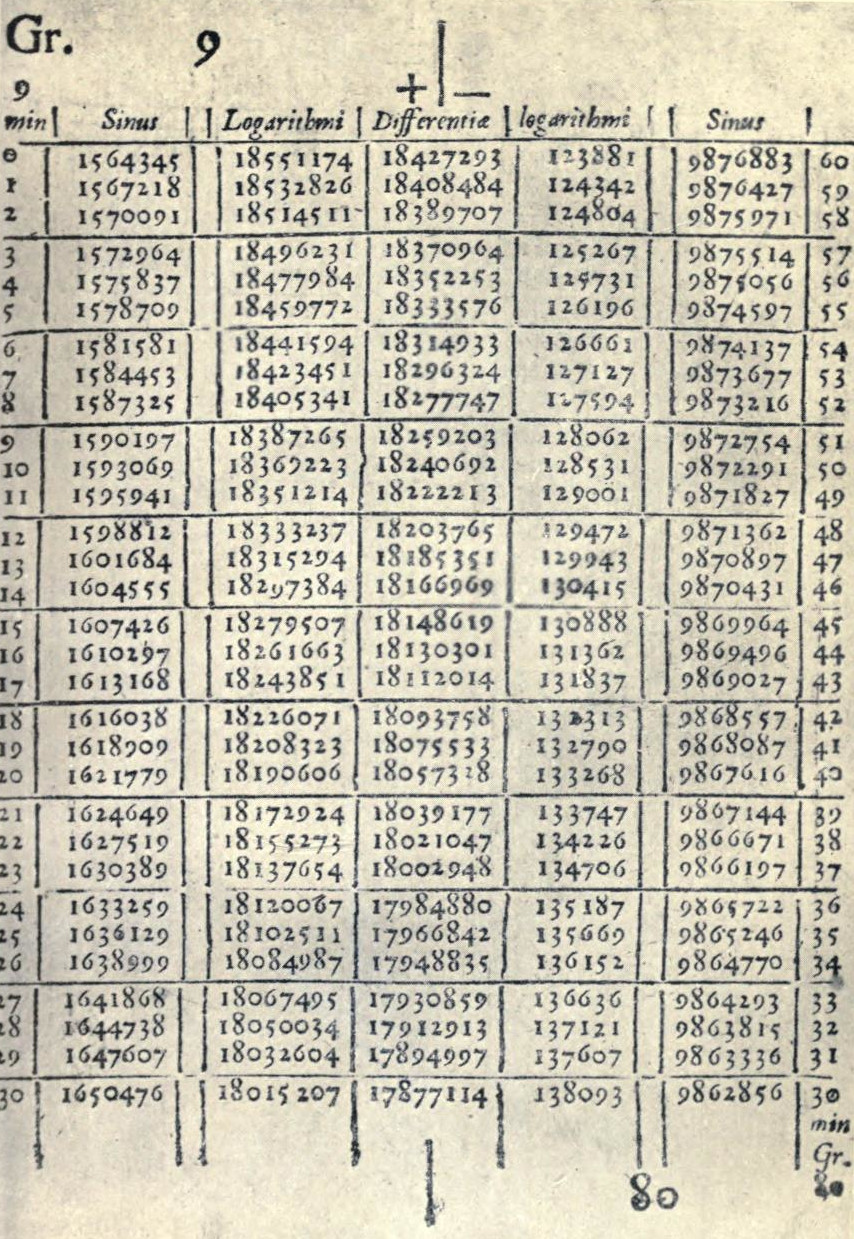
\includegraphics[width=10cm]{napier_tables.jpg}
  \end{center}
  \caption{Una pagina delle tavole calcolate da John Napier
  con i valori della funzione $\sin$ (Sinus) e del suo logaritmo
  (Logarithmi).
  In questa pagina ci sono i valori 
  per gli angoli dai 9 gradi (Gr.) ai 9 gradi e mezzo (i gradi 
  sessagesimali sono suddivisi in 60 minuti) e 
  dei loro complementari dagli 80 gradi e mezzo agli 81 gradi.
  Il codice scritto a pag.~\pageref{code:napier} permette
  di calcolare in pochi centesimi di secondo gli stessi valori
  mettendo anche in evidenza alcuni errori sulle ultime cifre decimali.
  Napier ci mise 20 anni a completare la stesura 
  delle tavole da 0 a 90 gradi.
  Se ad esempio volessimo calcolare il valore della tangente di $\alpha=9$ gradi 
  potremmo osservare che il logaritmo di $\tg \alpha$ 
  è la differenza tra il logaritmo di $\sin \alpha$ e il 
  logaritmo di $\cos \alpha$.
  Essendo il $\cos$ uguale al seno dell'angolo complementare 
  troviamo questo valore nella tabella in figura, 
  riga 0, colonna 
  \emph{Differenti\ae}: $1.8427293$ 
  (tutti i valori sono moltiplicati per $10^7$).
  Il valore cercato è l'esponenziale di questo 
  logaritmo e possiamo quindi calcolarlo cercando 
  lo stesso valore nella colonna \emph{Logarithmi}
  e prendendo il corrispondente valore nella colonna 
  \emph{Sinus}. Il valore è compreso tra i valori 
  della riga 6 e della riga 7. Più precisamente 
  differisce dal valore nella riga 7 
  $\frac{3842}{18143}$ volte quanto differisce il valore 
  della riga 6 dal valore della riga 7. 
  Applicando lo stesso rapporto ai valori trovati 
  nella colonna \emph{Sinus} si ottiene
  per interpolazione che al valore 
  della riga 7 (pari a 1.584453) và 
  sottratto 608 ottenendo quindi $\tg \alpha \approx 0.1583845$
  che differisce dal valore 
  esatto per meno di $10^{-7}$.
  }
  \label{fig:napier}
\end{figure}

\label{nota:Nepero}%
\index{Napier!John}%
\index{Nepero}%
\label{Euler!Leonhard}%
\label{Eulero}%
Nepero è l'italianizzazione del nome del
matematico scozzese \emph{John Napier} (1550-1617)
che per compilare le tavole della funzione seno
con una precisione di 7 cifre decimali ha introdotto 
per primo la funzione logaritmo (si veda la figura~\ref{fig:napier}).
E' interessante notare che Napier ha definito direttamente 
il logaritmo naturale senza introdurre il numero $e$ 
e senza fare alcun collegamento con la funzione esponenziale.
% https://archive.org/details/johnnapierinvent00hobsiala/page/18/mode/2up

\label{note:Bernoulli}%
\index{Bernoulli!Jacob}%
L'individuazione della costante $e$
è dovuta a \emph{Jacob Bernoulli} (1655--1705) nel 1683.
Bernoulli si chiedeva qual è l'interesse annuo effettivo
che si ottiene da un capitale che dia una rendita
giornaliera.
Se investo un capitale $c$ ad un tasso di interesse annuo 
pari a $r$, alla fine dell'anno mi viene restituito 
il capitale $c$ più un interesse $rc$.
Se divido il guadagno $rc$ per il numero di giorni che ci sono in 
un anno, posso considerare di aver avuto un guadagno giornaliero
pari a $\frac{r}{365} c$.
Se il guadagno giornaliero $\frac{r}{365} c$ mi venisse restituito 
immediatamente ogni giorno dell'anno, potrei reinvestire immediatamente 
il guadagno facendo aumentare il capitale durante l'anno.
In tal modo se parto con un capitale $c$ ogni giorno il mio capitale 
aumenterebbe di un fattore $1+\frac{r}{365}$ e
alla fine dell'anno avrei quindi un guadagno
pari a $\enclose{1+\frac{r}{365}}^{365} \approx e^r$ 
volte il capitale iniziale (interesse composto).

Il nome $e$ è stato introdotto da Eulero (Leonhard Euler 1707-1783).
%http://eulerarchive.maa.org//docs/originals/E853.pdf

\subsection{il teorema fondamentale dell'algebra}

La formula risolutiva per determinare le radici di un polinomio di secondo grado 
era già nota ai Babilonesi e sebbene i numeri complessi non erano noti 
(e neanche i numeri negativi) la stessa formula si applica 
nel caso generale e fornisce le radici complesse.

Lo studio delle equazioni di grado superiore al secondo si sviluppa invece 
nel 1500 ad opera dei matematici italiani Scipione del Ferro, 
Gerolamo Cardano, Niccolò Tartaglia e Lodovico Ferrari.
Essi determinano le formule risolutive per determinare le radici 
dei polinomi di terzo e quarto grado. 
Nell'applicare la formula risolutiva per l'equazione di terzo grado 
può capitare di dover calcolare la radice quadrata di un numero negativo
anche in situazioni in cui tutte le soluzioni alla fine risultano reali.
Ed è proprio in questo contesto che nascono i numeri complessi, come 
mero artificio matematico utilizzato per portare a termine il conto.

Successivamente Paolo Ruffini (1765-1822) e Niels Abel (1802-1829) dimostrarono che le equazioni 
di grado maggiore del quarto non ammettono una formula risolutiva 
esprimibile mediante radicali. 
Il criterio per determinare se un polinomio
ammette o meno formule risolutive è dovuto al matematico francese Évariste Galois
(1811-1832) che è considerato il fondatore della teoria dei gruppi.

Il teorema fondamentale dell'algebra, e cioè l'esistenza di radici 
complesse per polinomi di grado qualunque, viene dimostrato dal 
matematico tedesco Carl Friedrich Gauss (1777--1855). 
Questo teorema opera una svolta nel pensiero matematico in quanto 
per la prima volta si dà rilevanza ad un risultato astratto di esistenza 
slegato da una formula risolutiva. 
Il teorema non era affatto scontato, basti pensare che sia Leibniz 
che Nikolas Bernoulli erano convinti di aver trovato dei polinomi 
di quarto grado che non possono essere fattorizzati in contrasto 
con il teorema~\ref{th:fattorizzazione_polinomio_reale}.

\subsection{il problema isoperimetrico}

\label{note:isoperimetrico}%
\index{problema!isoperimetrico}%
Probabilmente già dal IX secolo a.C.\ era noto ai greci che 
la circonferenza, tra tutte le linee piane di lunghezza prefissata, 
è quella che racchiude la maggiore area (proprietà isoperimetrica).
Nell'Eneide Virgilio racconta che Didone si trovò ad affrontare 
un problema simile nella fondazione di Cartagine.
\index{Didone}%
\index{isoperimetrico!problema}%
\index{problema!isoperimetrico}%
\index{problema!di Didone}%
Salendo alla dimensione $n=3$ è naturale immaginare che 
la superficie che racchiude il volume maggiore con area fissata 
sia la sfera. 
Questo spiega il motivo per cui una goccia d'acqua, in assenza di gravità,
dovrebbe assumere una forma sferica: a causa della tensione superficiale, 
infatti, la superficie della goccia tenderà ad avere l'area minima.
Eulero (\emph{Leonhard Euler} 1707--1783)
\index{Euler!Leonhard}%
\index{Eulero}%
pensò di aver
trovato una dimostrazione
che si fondava su questo risultato:
presa una qualunque superficie chiusa nello spazio,
se questa non è una sfera è possibile
farne una piccola modifica in modo da ottenere una nuova superficie
che racchiude lo stesso volume ma che ha area strettamente inferiore.
Dirichlet (1805--1859) si accorse di un problema fondamentale 
nella dimostrazione di Eulero e nelle successive formalizzazioni di Steiner:
Eulero dimostrava che il minimo non può essere una superficie diversa dalla sfera,
ma non dimostrava che il minimo esiste.
Infatti Eulero dimostra che non ci può essere un minimo che non sia la sfera, 
ma non dimostra che il minimo esiste e quindi non è detto che la sfera sia il minimo: 
potrebbero esserci infinite superfici $S_1, S_2, \dots, S_n, \dots$ 
ognuna con area minore di quella della sfera e ognuna con area maggiore della successiva: 
$A(S_{n+1})< A(S_n)$. 
Per concludere il ragionamento di Eulero era necessario dimostrare 
che in una situazione del genere le superifici $S_n$ debbano, in qualche senso, 
tendere alla superficie sferica e che le loro aree debbano
tendere all'area della sfera. 
Karl Weiestrass (1815--1897)
\index{Weiestrass!Karl}%
si occupò di rifondare l'analisi in modo da rendere formali queste dimostrazioni.
La dimostrazione della proprietà isoperimetrica del cerchio e della sfera fu 
resa formale da Hermann Schwarz, 
\index{Schwarz!Hermann}%
uno studente della scuola di Weierstrass.
Il caso del cerchio viene usualmente attribuito a Steiner (1796--1863) in quanto 
sebbene non si fosse accorto, come Eulero, del problema dell'esistenza del minimo, 
aveva prodotto tutti gli strumenti necessari per completare la dimostrazione. 

La formulazione del problema isoperimetrico nella sua massima generalità 
(cioè per insiemi anche non regolari, e in dimensione qualunque)
è dovuta al matematico italiano Ennio De Giorgi (1928--1996)
\index{De Giorgi!Ennio}%
che formalizzò il concetto di perimetro introdotto
da Renato Caccioppoli (1904--1959).%
\index{Caccioppoli!Renato}%
\index{Caccioppoli!perimetro}%


\chapter{series}

Given a sequence $a_n$ of real or complex numbers, we can consider the sequence
of the so-called \emph{partial sums}%
\mymargin{partial sums}%
\index{sums!partial}
\[
  S_n = \sum_{k=0}^{n-1} a_k.
\]
\mynote{The sum starts from $k=0$ because we want to use all the terms of the sequence, but in many cases, the sequence will have its first index at $k=1$, and thus it will be natural to start from $k=1$. The last term is $n-1$ so that $S_n$ is the sum of the first $n$ terms of the sequence. Nothing would change if we chose $n$ instead of $n-1$.}
We can write more concisely $S_n = \sum a_n$.
Intuitively, it means summing the terms of the sequence $a_k$ for $k$ starting
from $0$ up to $k=n-1$:
\[
  \sum_{k=0}^{n-1} a_k = a_0 + a_1 + a_2 + \dots + a_{n-1}.
\]
Formally, the sum $S_n=\displaystyle \sum_{k=0}^n a_k$ is defined recursively by
the following relations:
\[
  \begin{cases}
    S_0 = 0, \\
    S_{n+1} = S_n + a_{n}.
  \end{cases}
\]

The numbers $a_n$ are called \emph{terms}%
\mymargin{terms}%
\index{term} of the series.
\index{terms!of a series}\index{series!terms}%
If the sequence of partial sums admits a limit, the limit is called the
\emph{sum}%
\mymargin{sum}%
\index{sum}
\index{sum!of a series}\index{series!sum}%
of the series and is denoted by
\[
  \sum_{k=0}^{+\infty} a_k 
  = \lim_{n\to +\infty} S_n 
  = \lim_{n\to+\infty} \sum_{k=0}^{n-1} a_k.
\]

The terminology already introduced for sequences also applies to series, which
are indeed sequences themselves. In particular, a series can be convergent,
divergent, or indeterminate. This is the \emph{nature of the series}.
\mymargin{nature}%
\index{nature!of a series}%
\index{series!nature}%

More generally, one can consider the sum starting from a certain index $m\in
\ZZ$. Given $m$, one can, for example, consider the series:
\[
  S_n = \sum_{k=m}^{n-1} a_k
\]
which is defined for every $n\in\NN$, $n\ge m$ as
\[
  S_n = a_m + a_{m+1} + \dots + a_{n-1}.
\]

\begin{example}
Consider the series $S_n$ defined as the sum of natural numbers from $1$ to $n$:
\[
  S_n 
  = \sum_{k=0}^{n-1} (k+1)
  = \sum_{k=1}^{n} k
  = 1 + 2 + \dots + n.
\]
We know that (exercise~\ref{ex:somma_lineare})
\[
  S_n = \frac{n(n+1)}{2}.
\]
And by the definition of limit, it can be verified that $S_n \to +\infty$.

This is expressed by saying that the series $\sum n$ is divergent:
\[
  \sum_{k=0}^{+\infty} (k+1)
  = \sum_{k=1}^{+\infty} k 
  = +\infty.
\]
\end{example}

\begin{example}[the geometric series]
Given $q \in \RR$ or $q\in \CC$, to the sequence
$  a_n = q^n$
of terms
\[
  a_0 = 1,\qquad
  a_1 = q,\qquad
  a_2 = q^2,\qquad
  a_3 = q^3, \dots
\]
is associated the
\emph{geometric series}%
\mymargin{geometric series}%
\index{series!geometric}
$\sum q^n$
whose partial sums are
\[
  S_0 = 0, \qquad
  S_1 = 1, \qquad
  S_2 = 1 + q, \qquad
  S_3 = 1 + q + q^2, \qquad
  \dots
\]
\end{example}

The following theorem shows us how, for different values of $q$, the geometric
series assumes all possible natures: convergent, divergent, indeterminate.

\begin{theorem}[sum of the geometric series]
\label{th:serie_geometrica}%
\mymark{***}%
\mymargin{sum of the geometric series}%
\index{sum!of the geometric series}%
Let $q\in \CC$. If $q\neq 1$, we have
\[
 \sum_{k=0}^{n-1} q^k  = \frac{1-q^n}{1-q}.
\]
If $\abs{q} < 1$, the geometric series converges:
\[
 \sum_{k=0}^{+\infty} q^k = \frac{1}{1-q}.
\]

If $\abs{q}\ge 1$, the series does not converge, but we must distinguish whether
the series is considered with real or complex values to determine its nature.

If we consider the series with real values (thus $q\in \RR$), if $q\ge 1$, the
series diverges to $+\infty$; if $q\le -1$, the series is indeterminate.

If we consider the series with complex values $q\in \CC$, if $\abs{q}>1$, the
series diverges to $\infty$, the same happens if $q=1$. If $\abs{q}=1$ but
$q\neq 1$, the series is indeterminate.
\end{theorem}
%
\begin{proof}
The first result concerns a finite sum. We have
\[
  (1-q)\cdot \sum_{k=0}^{n-1} q^k
  = \sum_{k=0}^{n-1} q^k - q \cdot \sum_{k=0}^{n-1} q^k
  = \sum_{k=0}^{n-1} q^k - \sum_{k=1}^{n} q^k
  = 1 - q^n
\]
from which, if $q\neq 1$, the desired result is obtained.

Taking the limit as $n\to +\infty$, if $\abs{q} < 1$, it is noted that
$\abs{q^n} = \abs{q}^{n} \to 0$, and the series thus converges to $\frac
1{1-q}$.

Now consider the series with real values. If $q>1$, we observe that $q^n\to
+\infty$, and thus the series diverges to $+\infty$ (in fact, in this case,
$1-q$ is negative). If $q=1$, we have $q^k=1$, and thus
$\displaystyle\sum_{k=0}^{n-1} q^k = n \to +\infty$.

For the other cases, we observe that
\[
  \sum_{k=0}^{n-1} q^k = \frac{1-q^n}{1-q}
  = \frac{1}{1-q} - \frac{1}{1-q}\cdot q^k
\]
and thus the nature of the series coincides with the nature of the sequence
$q^k$. If we consider the sequence with complex values and if $\abs{q}>1$, the
series is divergent to $\infty$ since $\abs{q^k}=\abs{q}^k\to +\infty$. If
instead, we consider the series with real values and $q<-1$ (the case $q\ge 1$
has already been considered), the series is indeterminate since in absolute
value it tends to $+\infty$, but the sign of the even terms is opposite to the
sign of the odd terms.

We still need to consider the case $\abs{q}=1$, $q\neq 1$. If $q$ is real, there
is only the case $q=-1$, and we know that $(-1)^k$ is indeterminate. Even if $q$
is complex, we want to show that the sequence $q^k$ is indeterminate: if it were
not, we would have $q^k\to \ell$ with $\abs{\ell}=1$ since $\abs{q^k}=1$, and
taking the limit in the equality
\[
  q^{k+2} = q\cdot q^{k+1}
\]
we would have $\ell = q\cdot \ell$, from which (dividing by $\ell$) we obtain
$q=1$. Thus, if $q\neq 1$, the sequence $q^k$ is indeterminate, and so is the
geometric series.
\end{proof}

\begin{theorem}[linearity of the sum]
\label{th:linearita_somma_serie}%
\mymargin{linearity of the infinite sum}%
\index{linearity of the infinite sum}
If $\sum a_n$ and $\sum b_n$ are convergent, then for every $\lambda,\mu\in \RR$
(or $\CC$), $\sum (\lambda a_n + \mu b_n)$ is also convergent, and we have
\[
 \sum_{k=0}^{+\infty} (\lambda a_n + \mu b_n)
 = \lambda \sum_{k=0}^{+\infty} a_n  + \mu \sum_{k=0}^{+\infty} b_n.
\]
\end{theorem}
%
\begin{proof}
If $S_n$ and $R_n$ are the partial sums of the series $\sum a_n$ and $\sum b_n$,
then the partial sums of the series $\sum (\lambda a_n + \mu b_n)$ are $\lambda
S_n + \mu R_n$ (since the distributive and commutative properties hold for
finite sums). But if $S_n \to S$ and $R_n \to R$, then $\lambda S_n + \mu R_n
\to \lambda S + \mu R$.
\end{proof}

We observe that series (like sequences) form a vector space in which the
operations of sum and scalar multiplication are performed term by term: $\sum
a_n + \sum b_n = \sum (a_n + b_n)$, $\lambda \sum a_n = \sum (\lambda a_n)$. The
previous theorem then tells us that convergent series (like convergent
sequences) form a subspace, and the sum of the series (like the limit of the
sequence) is a linear operator defined on this subspace.

\begin{theorem}[necessary condition for convergence]
\mymark{***}
\mymargin{necessary condition}%
\index{necessary condition}
If the series $\sum a_n$ converges, then $a_n \to 0$.
\end{theorem}
%
\begin{proof}
\mymark{***}
If the series $\sum a_n$ converges, it means that the partial sums $S_n =
\displaystyle\sum_{k=0}^{n-1} a_k$ converge: $S_n \to S$. But then
\[
  a_n = S_n - S_{n-1} \to S - S = 0.
\]
\end{proof}

\begin{theorem}[stability of the nature]%
\index{nature!of a series}%
\index{stability!of the nature}%
\index{series!stability of the nature}%
\index{series!that differ on a finite number of terms}%
If the two sequences $a_n$ and $b_n$ differ only on a finite number
\mymargin{stability of the nature}%
of terms, then the corresponding series $\sum a_n$ and $\sum b_n$ have the same
nature.
\end{theorem}
%
\begin{proof}
If the sequences differ on a finite number of terms, it means that there exists
an $N\in \NN$ such that for every $k>N$, we have $a_k=b_k$. Thus, if we denote
by $S_n = \sum_{k=0}^{n-1} a_k$ and $R_n = \sum_{k=0}^{n-1} b_k$ the
corresponding sequences of partial sums, for every $n>N$, we have
\[
  S_n - R_n
    = \sum_{k=0}^{n-1} a_k - \sum_{k=0}^{n-1} b_k
    = \sum_{k=0}^{N-1} (a_k - b_k) 
    = C
\]
where $C$ is a constant independent of $n$. Therefore, for $n>N$, we have
\[
  S_n = R_n + C.
\]
If the limit of $R_n$ does not exist, then the limit of $S_n$ does not exist
either (otherwise, since $R_n = S_n -C$, the limit of $R_n$ should also exist).
If the limit of $R_n$ is infinite, then the limit of $S_n$ is equal to the limit
of $R_n$. And if the limit of $R_n$ is finite, then the limit of $S_n$ is also
finite.

Thus, the nature of the sequence $S_n$ is the same as that of the sequence
$R_n$, i.e., the two series have the same nature.
\end{proof}

If a series has its first term with an index different from $0$, one can always
reduce it (with a change of variable) to a series whose index starts from zero.
For example (making the change of variable $j=k-1$ from which $j=0$ when $k=1$
and remembering that the index used in the sums of the series is a dummy
variable):
\[
 \sum_{k=1}^{+\infty} \frac{1}{2^k}
 = \sum_{j=0}^{+\infty} \frac{1}{2^{j+1}}
 = \sum_{k=0}^{+\infty} \frac{1}{2^{k+1}}.
\]

It should also be noted that according to the previous theorem, the first index
from which one starts summing is not relevant concerning the nature of the
series. However, if the series is convergent, its sum may vary, for example:
\[
 \sum_{k=1}^{+\infty} \frac{1}{2^k}
 = \enclose{\sum_{k=0}^{+\infty} \frac{1}{2^k}} - 2^0.
\]

Note well: in many books, $\infty$ is written instead of $+\infty$. It is
therefore very common to omit the $+$ sign in front of $\infty$ in the
terminology of series (and also sequences) since the indices are understood to
be natural numbers, and thus $-\infty$ would not make sense.

However, there are cases where it may be useful to use negative indices, for
example, if $a_k$ is defined for every $k\in \ZZ$, one could define (but we will
not do so):
\[
  \sum_{k=-\infty}^{+\infty} a_k
  = \sum_{k=0}^{+\infty} a_k +
  \sum_{k=1}^{+\infty} a_{(-k)}
\]
requiring that both series on the right side of the equality exist and do not
have infinite sums of opposite signs.

\begin{theorem}[tail of a convergent series]
\label{th:coda}%
\mymark{*}%
Let $\sum a_n$ be a convergent series. Then
\[
  \lim_{n\to +\infty} \sum_{k=n}^{+\infty} a_k = 0.
\]
\end{theorem}
%
\begin{proof}
\mymark{*}
Let
\[
  S_n = \sum_{k=0}^{n-1} a_k,
\]
by the definition of a convergent series, we know that there exists a finite $S$
such that $S_n \to S$. We then observe that
\[
  \sum_{k=n}^{+\infty} a_k = \lim_{N\to+\infty} \sum_{k=n}^{N-1} a_k
   = \lim_{N\to +\infty} S_N - S_n = S - S_n
\]
and, for $n\to +\infty$, we obviously have $S - S_n \to S - S = 0$.
\end{proof}
\section{Telescopic Series}

A series written in the form
\[
  \sum (a_{k} - a_{k+1})
\]
is called \emph{telescopic}
\mymargin{telescopic series}%
\index{series!telescopic}
because the individual terms of the sum (like the tubes of a telescope),
cancel each other out (allowing the telescope to close):
\[
  S_n 
  = \sum_{k=0}^{n-1} (a_{k} - a_{k+1})
  = \sum_{k=0}^{n-1} a_k - \sum_{k=1}^{n} a_k
  = a_0 - a_n.
\]

In theory, any series can be written in telescopic form,
given $S_n$, it suffices to choose $a_n=-S_n$, 
so that the previous relation holds. 
Writing a series in telescopic form is therefore equivalent to 
determining the sequence of partial sums.

\begin{example}[Mengoli's series]
\mymark{**}
We have
\[
  \sum_{n=1}^{+\infty} \frac{1}{n(n+1)} = 1.
\]
\end{example}
%
\begin{proof}
\mymark{**}
Indeed,
\[
  \sum_{k=1}^n \frac{1}{k(k+1)}
  = \sum_{k=1}^n \enclose{\frac{1}{k} - \frac{1}{k+1}}
  = \sum_{k=1}^n \frac{1}{k} - \sum_{k=2}^{n+1} \frac{1}{k}
  = 1 - \frac{1}{n+1} \to 1.
\]
\end{proof}
\section{series with positive terms}

\index{series!with positive terms}
In the following, we will consider series whose terms are positive real numbers
(or at least non-negative).
When we write $a_n >0$ (or $a_n \ge 0$), it will always be implied that $a_n\in
\RR$ since for non-real complex numbers we have not defined the order relation.

\begin{theorem}[nature of series with positive terms]\label{th:serie_positiva}
\mymark{***}%
\mymargin{nature of series with positive terms}%
\index{nature!of a series with positive terms}%
If $a_n\ge 0$, the series $\sum a_n$ is regular:
either it converges or it diverges to $+\infty$.
\end{theorem}
%
\begin{proof}
\mymark{***}
If $a_n \ge 0$, since $S_{n+1} = S_n + a_n$, it means that the sequence $S_n$ of
partial sums is increasing.
Thus, the limit of $S_n$ exists and cannot be negative.
\end{proof}

\begin{theorem}[comparison test]
\mymark{**}
\mymargin{comparison test}
\index{test!comparison for series}
Let $\sum a_n$ and $\sum b_n$ be series with positive terms that are compared:
$0\le a_n\le b_n$.
Then
\[
  \sum_{k=0}^{+\infty} a_k \le \sum_{k=0}^{+\infty} b_k.
\]
In particular, if $\sum b_n$ converges, then $\sum a_n$ also converges, and if
$\sum a_n$ diverges, then $\sum b_n$ also diverges.

This latter result holds even if $0 \le a_n \ll b_n$.
\end{theorem}
%
\begin{proof}
\mymark{*}
If $S_n$ are the partial sums of $\sum a_n$ and $R_n$ are the partial sums of
$\sum b_n$, we have $S_n \le R_n$, and the result reduces to the comparison
between sequences.

In the case where $a_n \ll b_n$, by definition, we know that $\frac{a_n}{b_n}\to
0$, and therefore, from the definition of limit, we know that there exists $N$
such that for every $n>N$, we have (having chosen $\eps=1$)
\[
  \frac{a_n}{b_n} < 1.
\]
Thus, we obtain $a_n \le b_n$ for all $n$ except at most a finite number.
Knowing that the nature of the series does not change if the series is modified
on a finite number of terms, we reduce to the previous case.
\end{proof}

\begin{example}\label{ex:52573}
\mymark{***}
The series
\begin{equation}\label{eq:296453}
 \sum_{k=1}^{+\infty} \frac{1}{k^2}
\end{equation}
is convergent.
Indeed, observing that for every $n>0$, we have
\[
  \frac{1}{(n+1)^2} \le \frac{1}{n(n+1)}
\]
we can assert that
\[
  \sum_{k=1}^{+\infty} \frac{1}{k^2}
  = 1 + \sum_{k=1}^{+\infty} \frac{1}{(k+1)^2}
  \le 1+ \sum_{k=1}^{+\infty} \frac{1}{k(k+1)}
  = 2
\]
since we have reduced to the telescopic series of Mengoli, which has a sum equal
to $1$.

We thus know that the series~\eqref{eq:296453} is convergent without knowing
exactly what its sum is.
However, we can numerically find approximations of the sum by summing the first
terms and estimating the error using the series of Mengoli, whose sum we know
how to calculate.
Indeed, if $S_N$ is the partial sum of the first $N$ terms and $S = \lim S_N$ is
the sum of the series, since $1/(k+1)^2 \le 1/(k^2+k)$, we have
\[
S_N
\le S
\le S_N + \sum_{k=N}^{+\infty} \frac{1}{k(k+1)}
\le S_N + \frac{1}{N}.
\]
To calculate the first 6 exact decimal places, it will suffice to sum the first
million terms of the series.
This can be done, for example, with the code provided on
page~\pageref{code:series}, obtaining $S\approx 1.644934$.

Using much more advanced tools, Euler \index{Euler}
(Leonard Euler, 1707--1783) managed to express the sum of this series using
fundamental mathematical constants (we will do so with a different method in
exercise~\ref{ex:Basilea}).
\end{example}

\begin{corollary}[asymptotic comparison test]
\mymark{*}
\mymargin{asymptotic comparison test}
\index{test!asymptotic comparison}
If $a_n$ and $b_n$ are sequences with positive terms, asymptotically equivalent
(definition~\ref{def:ordine_infinito}), then the corresponding series $\sum a_n$
and $\sum b_n$ have the same nature.
\end{corollary}
%
\begin{proof}
\mymark{*}
Series with positive terms cannot be indeterminate, so it is sufficient to
verify that if one series converges, the other also converges.
Since $a_n / b_n$ is convergent, this ratio must also be bounded
(theorem~\ref{th:limitatezza_successione_convergente}), so there exists $C\in
\RR$ such that
\[
   a_n \le C \cdot b_n.
\]
If the series $\sum b_n$ converges, then $\sum C \cdot b_n$ also converges, and
by comparison, $\sum a_n$ also converges.

Conversely, by swapping the roles of $a_n$ and $b_n$, we verify that if $a_n$
converges, then $b_n$ also converges.
\end{proof}

\begin{example}
The series
\[
\sum_n \frac{n^2+2n+3}{2n^4-n^3+n+1}
\]
is convergent. Indeed, it can be easily verified that
\[
   \frac{n^2+2n+3}{2n^4-n^3+n+1} \sim \frac{1}{2n^2}.
\]
But we know that the series $\sum 1/n^2$ is convergent, consequently, the series
$\sum 1/(2n^2)$ is also convergent (by the linearity of the sum,
theorem~\ref{th:linearita_somma_serie}), and therefore, by asymptotic
comparison, the given series is also convergent.
\end{example}

In chapter \ref{sec:serie_segno_variabile}, we will see that the asymptotic
convergence test can only be applied to series with positive terms.

\begin{theorem}[root test]
\mymargin{root test}
\index{test!root}
Let $\sum a_n$ be a series with non-negative terms (i.e., $a_n\ge 0$) such that
\mymark{***}
$\sqrt[n]{a_n} \to \ell \in [0,+\infty]$.
If $\ell<1$, then the series converges.
If $\ell>1$, then the series diverges.

More generally, the result is valid with
\[
  \ell = \limsup \sqrt[n]{a_n}
\]
even in the case where the limit of $\sqrt[n]{a_n}$ does not exist.
\end{theorem}
%
\begin{proof}
\mymark{***}
In the case $\ell < 1$, we take $q$ with $\ell < q < 1$ and set $\eps = q-\ell$.
By the definition of limit $\sqrt[n]{a_n}\to \ell$ (but it suffices that
$\limsup \sqrt[n]{a_n}=\ell$), we know there exists $N$ such that for every $n >
N$, we have
\[
  \sqrt[n]{a_n} < \ell + \eps = q
\]
that is
\[
   a_n < q^n.
\]
Knowing that $\sum q^n$ converges, and knowing that the nature of the series
does not change by modifying a finite number of terms, by comparison, we can
conclude that the series $\sum a_n$ also converges.

If $\ell>1$, we have that $\sqrt[n]{a_n}>1$ and therefore $a_n>1$ for infinitely
many values of $n$. The sequence $a_n$ is not infinitesimal, and thus the series
cannot converge.
\end{proof}

\begin{example}
The series
\[
  \sum_k 2^{(\ln k) - k}
\]
is convergent. Indeed, we have
\[
 \sqrt[k]{2^{\ln k - k}}
 = 2^{\frac{\ln k - k}{k}}
 = 2^{\frac{\ln k }k - 1}
 \to 2^{-1}
 = \frac{1}{2}
 < 1.
\]
\end{example}

\begin{theorem}[ratio test]
\mymark{***}
\mymargin{ratio test}
\index{test!ratio for series}
Let $\sum a_n$ be a series with positive terms ($a_n > 0$) such that $a_{n+1} /
a_n \to \ell \in [0,+\infty]$.
If $\ell <1$, then the series converges.
If $\ell > 1$, the series diverges.
\end{theorem}
%
\begin{proof}
\mymark{*}
It would not be difficult to provide a direct proof, similar to the proof given
for the root test.
However, we can observe that by the Cesàro convergence criterion
(theorem~\ref{th:criterio_cesaro}), we have $\sqrt[n]{a_n} \to \ell$, so we
reduce to the root test without needing further proofs.
\end{proof}

\begin{example}
\mymark{***}
For every $x\ge 0$, the series
\[
  \sum \frac{x^n}{n!}
\]
converges.
\end{example}
%
\begin{proof}
We apply the ratio test.
Setting $a_n = x^n / n!$, we have
\[
\frac{a_{n+1}}{a_n}
= \frac{x^{n+1}}{(n+1)!}\cdot \frac{n!}{x^n}
= \frac{x}{n+1} \to 0 < 1.
\]
Thus, the series converges.
\end{proof}

\subsection{associativity of the sum of a series}

\begin{example}
Setting $a_k = (-1)^k$, we know that the corresponding series:
\[
  1 - 1 + 1 - 1 + 1 \dots
\]
is indeterminate because the partial sums are
\[
  S_n = \sum_{k=0}^n (-1)^k
  = \begin{cases}
   1 & \text{if $n$ is even}\\
   0 & \text{if $n$ is odd.}
  \end{cases}
\]
However, if we associate the terms in pairs, we obtain the series
\[
  (1-1) + (1-1) + (1-1) \dots = 0 + 0 + 0 + \dots = 0
\]
which is convergent.
The reason is that the sequence of partial sums of this new series is a
particular subsequence (the one with even indices) of the sequence of partial
sums of the original series. Therefore, it should not surprise us that even
though the original series was indeterminate, it is possible to associate the
terms of the series in such a way as to obtain a regular series (in this case,
convergent).
In fact, by the Bolzano-Weierstrass theorem~\ref{th:bolzano_weierstrass}, we
know that it is always possible to extract a regular (convergent or divergent)
subsequence from any sequence.
Even when a convergent series is extracted from an indeterminate series, the sum
of the series can depend on how the terms are associated.
For example, in the previous series, if we only took the sums with odd indices,
we would obtain:
\[
  1 + (-1+1) + (-1+1) + \dots = 1.
\]
\end{example}

The previous example shows us that by associating the terms of an indeterminate
series, it is possible to obtain series with different nature and sum.
The following theorem tells us that this "bad" phenomenon can only occur when
starting from an indeterminate series.
If the series is regular, then we can associate its terms without changing
either its nature or its sum.
In particular, this is true for series with positive terms.

\begin{theorem}[associativity of regular series]%
\label{th:serie_associativa}%
If $\sum a_k$ is a series, choosing any increasing sequence $k_n$ with $k_0=0$,
we can consider the series $\sum b_n$ whose terms
\[
  b_n = \sum_{j=k_n}^{k_{n+1}-1} a_j
\]
are obtained by associating the terms of $a_k$ into consecutive groups delimited
by the sequence of indices $k_n$.

If the series $\sum a_k$ is regular (convergent or divergent), then the series
$\sum b_n$ is also regular, and we have
\[
\sum_{n=0}^{+\infty} b_n
= \sum_{k=0}^{+\infty} a_k.
\]

In particular, this holds if the series $\sum a_k$ is with positive terms.
\end{theorem}
%
\begin{proof}
Let $S_k = \sum_{j=0}^k a_j$ be the partial sums of the series $\sum a_j$. Then
the partial sums of the series $\sum b_n$ are nothing but the subsequence
$S_{k_n}$.
Thus, if $S_k$ converges, every subsequence of it also converges to the same
limit.

The theorem~\ref{th:serie_positiva} tells us that series with positive terms are
regular and therefore satisfy the hypotheses of the theorem.
\end{proof}

\subsection{the harmonic series}

We observe that the ratio test does not apply to the \emph{harmonic series}%
\mymargin{harmonic series}%
\index{series!harmonic}%
\[
  \sum_k \frac{1}{k}
\]
since
\[
 \frac{\frac{1}{k+1}}{\frac{1}{k}}
 = \frac{k}{k+1} \to 1.
\]

To understand whether the harmonic series converges or diverges, we present the
method of \emph{condensation}, which will be stated in general in the next
theorem but can be better understood when applied to the particular case of the
harmonic series.

We will show that the harmonic series diverges.
The idea is simply to associate the terms of the harmonic series into groups of
length powers of two and estimate the sum of each group from below with the
smallest term (i.e., the last) of each group:
\begin{align*}
 \sum_{k=1}^{+\infty} \frac{1}{k}
 & = 1 + \frac 1 2
     + \enclose{\frac 1 3 + \frac 1 4}
     + \enclose{\frac 1 5 + \frac 1 6 + \frac 1 7 + \frac 1 8}
     + \dots\\
 & > 1 + \frac 1 2 + 2 \cdot \frac 1 4 + 4 \cdot \frac 1 8 + \dots \\
   & = 1 + \frac 1 2 + \frac 1 2 + \frac 1 2 + \dots
    = +\infty.
\end{align*}

\begin{theorem}[Cauchy's condensation test]%
\label{th:condensazione}%
\mymark{**}%
\mymargin{Cauchy's condensation test}%
\index{test!Cauchy's condensation}%
\index{condensation!Cauchy's test}%
\index{Cauchy!condensation test}%
Let $a_n$ be a decreasing sequence of non-negative real numbers: $a_n \ge 0$.
Then the series $\sum a_k$ converges if and only if the series
\[
  \sum 2^k a_{2^k}
\]
converges.
\end{theorem}
%
\begin{proof}
\mymark{**}
For convenience, suppose the sums start from $k=1$.
It involves grouping the terms $a_k$ into groups of powers of two:
\begin{align*}
  b_0 & = a_1, \\
  b_1 &= a_2 +  a_3, \\
  b_2 &= a_4 +  a_5 +  a_6 +  a_7, \\
  b_3 &= a_8 +  a_9 +  a_{10} + \dots + a_{15}, \\
  &\vdots\\
  b_n &= a_{2^n} +  a_{2^{n}+1} + \dots + a_{2^{n+1}-1},\\
  &\vdots
\end{align*}
Thanks to theorem~\ref{th:serie_associativa} on the associativity of series with
positive terms, we know that
  \[
  \sum_{k=1}^{+\infty} a_k = \sum_{n=0}^{+\infty} b_n.
  \]
Each term $b_n$ is the sum of $2^n$ terms of the sequence $a_k$, which, being a
decreasing sequence, can be estimated from above and below with the first and
last term of each sum, thus:
\[
  2^n a_{2^{n+1}-1} \le b_n \le 2^n a_{2^{n}}.
\]
By hypothesis, the series $\sum 2^n a_{2^n}$ is convergent, so by comparison,
the series $\sum b_n$ is also convergent.

Conversely, if the series $\sum 2^n a_{2^n}$ is divergent, then the series $\sum
2^{n+1} a_{2^{n+1}}$ is also divergent, and knowing that $b_n\ge 2^n
a_{2^{n+1}-1}\ge \frac 1 2 2^{n+1} a_{2^{n+1}}$, we obtain, by comparison, that
the series $\sum b_n$ is also divergent.
\end{proof}

\begin{corollary}[generalized harmonic series]
\mymark{***}
\mymargin{generalized harmonic series}%
\index{series!harmonic!generalized}
The series
\[
 \sum_n \frac{1}{n^\alpha}
\]
converges if $\alpha>1$,
diverges if $0\le \alpha\le 1$.
\end{corollary}
%
\begin{proof}
\mymark{***}
We apply the condensation test. Setting $a_n = \frac 1{n^\alpha}$, we have
\[
  \sum_n 2^n a_{2^n} = \sum_n 2^n \frac{1}{(2^n)^\alpha}
  = \sum_n 2^{n(1-\alpha)}
  = \sum_n \enclose{2^{(1-\alpha)}}^n
\]
which is a geometric series with ratio $q=2^{1-\alpha}$.
If $\alpha>1$, then $q<1$, and the harmonic series is convergent; if $\alpha \le
1$, then $q\ge 1$, and the harmonic series is divergent.
\end{proof}

\begin{exercise}
Use the condensation test to prove that the series
\[
  \sum \frac{1}{n \cdot \ln n}
\]
diverges.
\end{exercise}

\begin{exercise}
    Determine the values of the parameters $\alpha\in \RR$ and $\beta\in \RR$
  for which the following series is convergent:
  \[
    \sum \frac{1}{n^\alpha (\ln n)^\beta}.
  \]
\end{exercise}
\section{Positional Representation of Real Numbers}
\label{sec:decimali}
%%%
%%%
When we write $\frac{3}{8} = 0.375$, we mean that it holds 
\[
\frac 3 8 = \frac{3}{10} + \frac{7}{10^2} + \frac{5}{10^3}.  
\]
More generally, given a base $d\in \NN$, $d\ge 2$, ($d=10$ in 
the case of decimal representation), we consider the set $\Enclose{d} =
\ENCLOSE{0,1,2,\dots, d-1}$
of digits in base $d$.
An infinite sequence of digits will thus be an element 
$\vec a \in \Enclose{d}^\NN$, $\vec a = (a_0,a_1,\dots, a_n, \dots)$
with $a_k\in \Enclose{d}$.
We can then consider the number ``$0.a_0 a_1 a_2 \ldots$'' represented 
by the sequence of digits $\vec a$:
\[
  r(\vec a) = \sum_{k=0}^{+\infty} \frac{a_k}{d^{k+1}}.
\]
Clearly, $r(\vec a)\in [0,1]$ since, given $0\le a_k\le d-1$, 
it follows that
\begin{equation}\label{eq:10445934}
 0 \le r(\vec a) \le \sum_{k=0}^{+\infty} \frac{d-1}{d^{k+1}}
  = \frac{d-1}{d}\sum_{k=0}^{+\infty}\frac 1 {d^k}
  = \frac{d-1}{d}\cdot \frac{1}{1-\frac 1 d} = 1.
\end{equation}

Every number $x\in [0,1)$ admits a representation in digits $x=r(\vec a)$ 
with $\vec a \in \Enclose{d}^\NN$. 
Indeed, for every $N\in \NN$, we can write 
\[
  \lfloor x\cdot 10^N \rfloor= \sum_{k=0}^{N-1} a_k 10^{N-1-k}
\]
and as $N$ increases, we obtain a sequence of digits $a_k\in \Enclose{d}$ 
such that 
\[
  \abs{x \cdot d^N - \sum_{k=0}^{N-1} a_k \cdot d^{N-1-k}} \le 1
\]
from which 
\[
  \abs{x - \sum_{k=0}^{N-1} \frac{a_k}{d^{k+1}}} \le \frac{1}{d^{N}}
\]
which, letting $N\to +\infty$, implies $r(\vec a) = x$.
The number $x=1$ can also be represented by taking 
$a_k=d-1$ for every $k\in \NN$, thus achieving equality 
on the right side of \eqref{eq:10445934}. 
In base $d=10$, this is expressed by saying that 
\[
 0.999\ldots = 1.  
\]

We may ask whether it is possible for the same number 
to have two distinct representations in digits.
Suppose, therefore, that there exist $\vec a,\vec b\in \Enclose{d}^\NN$
with $\vec a \neq \vec b$ 
such that $r(\vec a) = r(\vec b)$. 
Let $m = \min\ENCLOSE{n\in\NN\colon a_n\neq b_n}$ be the position 
of the first differing digit between $\vec a$ and $\vec b$.
Then we have 
\[
 r(b) - r(a) = \sum_{k=0}^{+\infty}\frac{b_k - a_k}{d^{k+1}}
 = \frac{b_m - a_m}{d^{m+1}} + \sum_{k=m+1}^{+\infty} \frac{b_k - a_k}{d^{k+1}}
 = A+B
\]
with 
\[
\abs{A} = \abs{\frac{b_m - a_m}{d^{m+1}}} \ge \frac{1}{d^{m+1}}  
\]
and 
\begin{align*}
\abs{B} &= \abs{\sum_{k=m+1}^{+\infty} \frac{b_k - a_k}{d^{k+1}}}
        \le \sum_{k=m+1}^{+\infty} \frac{d-1}{d^{k+1}}\\
        &= \frac{d-1}{d^{m+2}}\sum_{k=0}^{+\infty}\frac{1}{d^k}
        = \frac{d-1}{d^{m+2}}\cdot \frac{1}{1-\frac 1 d} = \frac{1}{d^{m+1}}.
\end{align*}
Thus, by the reverse triangle inequality,
\[
0 = \abs{r(b)-r(a)}\ge \abs{A} - \abs{B} \ge 0.  
\]
This means that all inequalities are, in fact, equalities,
and thus it must be $\abs{b_m-a_m}=1$ 
and for every $k>m$, it must be $\abs{b_k-a_k}=d-1$. 
Assuming $b_m=a_m+1$ (the other case is analogous),
for $k>m$, it must necessarily be $b_k=0$ and $a_k=d-1$.

For example, if $d=10$, $\vec a = (1,2,3,9,9,9,9,\dots )$ 
and $\vec b = (1,2,4,0,0,0,0,\dots)$, we will have 
$r(\vec a) = r(\vec b) = 0.124$.
\section{absolute convergence}

For series with positive terms, we have many convergence criteria that, in
general, do not apply to series with arbitrary signs or to series of complex
numbers. However, the convergence of the latter can sometimes be easily reduced
to the convergence of series with positive terms by considering the modulus of
each term.

\begin{definition}[absolute convergence]
\mymark{***}
We say that a series (with real or complex terms) $\sum a_n$ is \emph{absolutely
convergent}%
\mymargin{absolutely convergent}%
\index{absolutely!convergent} if the series $\sum \abs{a_n}$ is convergent.
\end{definition}

\begin{theorem}[absolute convergence]\label{th:convergenza_assoluta}
\mymark{***}%
If a series $\sum a_n$ (real or complex) is absolutely convergent, then it is
convergent and the following holds:
\[
  \abs{\sum_{k=0}^{+\infty} a_k} \le \sum_{k=0}^{+\infty} \abs{a_k}.
\]
\end{theorem}
%
\begin{proof}
\mymark{*}
Initially, suppose that the $a_n$ are real numbers. Define $a_n^+ =
\max\ENCLOSE{0, a_n}$ and $a_n^- = -\min \ENCLOSE{0, a_n}$. That is, if $a_n\ge
0$, then $a_n^+ = a_n$ and $a_n^-=0$; if $a_n\le 0$, then $a_n^+ =0$ and $a_n^-
= -a_n$. Thus, $a_n^+\ge 0$, $a_n^-\ge 0$,
\[
   a_n = a_n^+  - a_n^-
   \qquad\text{and}\qquad
   \abs{a_n} = a_n^+ + a_n^-.
\]
Then, if $\sum \abs{a_n}$ converges, by comparison, both $\sum a_n^+$ and $\sum
a_n^-$ converge. Therefore, by the theorem on the sum of limits, $\sum a_n =
\sum a_n^+ - \sum a_n^-$, and hence $\sum a_n$ also converges.

If we have a sequence of complex numbers $a_n = x_n + i y_n$ and if $\sum
\abs{a_n}$ converges, then by comparison, both $\sum \abs{x_n}$ and
$\sum\abs{y_n}$ converge (note that $\abs{x} \le \abs{x+iy}$ and $\abs{y}\le
\abs{x+iy}$). Thus, $\sum x_n$ and $\sum y_n$ converge by what has already been
demonstrated for series with real terms. But then $\sum i y_n$ and $\sum a_n =
\sum (x + iy_n)$ also converge.

Now, let us set
\[
  S_n  = \sum_{k=0}^n a_k.
\]
By the subadditivity of the modulus, we know that for finite sums, we have
\[
 \abs{S_n} =\abs{\sum_{k=0}^n a_k}
 \le \sum_{k=0}^n \abs{a_k} \le \sum_{k=0}^{+\infty} \abs{a_k}.
\]
And by the continuity of the modulus, setting $S= \lim S_n$, we have
\[
  \abs{\sum_{k=0}^{+\infty} a_k}
  = \abs{S}
  = \lim_{n\to +\infty} \abs{S_n}
  \le \sum_{k=0}^{+\infty} \abs{a_k}.
\]
\end{proof}

\begin{theorem}[exchange of series]
\label{th:scambio_somma}
Let $a_{k,j}\in \RR$ or $a_{k,j}\in \CC$ be a two-index sequence $k\in \NN$,
$j\in \NN$. If
\begin{equation}\label{eq:499655}
  \sum_{k=0}^{+\infty}\sum_{j=0}^{+\infty}\abs{a_{k,j}}<+\infty  
  \qquad \text{or} \qquad
  \sum_{j=0}^{+\infty}\sum_{k=0}^{+\infty}\abs{a_{k,j}}<+\infty  
\end{equation}
then
\begin{equation}\label{eq:scambio_somma}
  \sum_{k=0}^{+\infty} \sum_{j=0}^{+\infty} a_{k,j}
  = \sum_{j=0}^{+\infty} \sum_{k=0}^{+\infty} a_{k,j}.
\end{equation}
\end{theorem}
%
\begin{proof}
Since the statement is symmetric in $k$ and $j$, we can assume that the first of
the two alternatives in hypothesis~\eqref{eq:499655} is satisfied: $\sum_k
\sum_j \abs{a_{k,j}}<+\infty$.

It is understood, of course, that for each $k$, the series $\sum_j
\abs{a_{k,j}}$ is convergent, hence $\sum_j a_{k,j}$ is absolutely convergent.
% and, by theorem~\ref{th:convergenza_assoluta}, 
% also $\sum_k \abs{\sum_j a_{k,j}} 
% \le \sum_k \sum_j \abs{a_{k,j}}$
% is absolutely convergent.
Obviously, 
$\sum_k \abs{a_{k,j}} \le \sum_k \sum_j \abs{a_{k,j}}$
and thus for each $j$, the series 
$\sum_k a_{k,j}$ is also absolutely convergent.
Setting
\[
S = \sum_{k=0}^{+\infty}\sum_{j=0}^{+\infty} a_{k,j},
\qquad
S_n = \sum_{j=0}^{n-1}\sum_{k=0}^{+\infty} a_{k,j}  
\]
we need to show that $S_n \to S$
as $n\to +\infty$. 
We apply the definition of limit:
let $\eps>0$ be fixed.
By the tail theorem~\ref{th:coda}, there exists $K$ such that 
\[
  \sum_{k=K}^{+\infty} \sum_{j=0}^{+\infty} \abs{a_{k,j}}<\frac \eps 2
\]
and for each $k<K$, there exists $J_k$ such that 
\[
  \sum_{j=J_k}^{+\infty} \abs{a_{k,j}} < \frac{\eps}{2K}.  
\]
Thus, setting $J=\max\ENCLOSE{J_0,J_1, \dots, J_{K-1}}$, if $n>J$, we have:
\begin{align*}
  \abs{S-S_n}
  &= \abs{\sum_{k=0}^{+\infty}\sum_{j=0}^{+\infty}a_{k,j} 
  - \sum_{j=0}^{n-1}\sum_{k=0}^{+\infty}a_{k,j}}
  = 
  \abs{\sum_{k=0}^{+\infty}\sum_{j=0}^{+\infty}a_{k,j} 
  - \sum_{k=0}^{+\infty}\sum_{j=0}^{n-1}a_{k,j}}\\
  &=
  \abs{\sum_{k=0}^{+\infty}\sum_{j=n}^{+\infty}a_{k,j} }
  = \abs{\sum_{k=0}^{K-1}\sum_{j=n}^{+\infty} a_{k,j}
   + \sum_{k=K}^{+\infty}\sum_{j=n}^{+\infty} a_{k,j}}\\
   &\le \sum_{k=0}^{K-1}\sum_{j=n}^{+\infty} \abs{a_{k,j}}
    + \sum_{k=K}^{+\infty}\sum_{j=0}^{+\infty} \abs{a_{k,j}}
   \le \sum_{k=0}^{K-1}\sum_{j=J_k}^{+\infty} \abs{a_{k,j}}
   + \frac \eps 2
  \le \frac \eps 2 + \frac \eps 2 = \eps
\end{align*}
as we wanted to demonstrate.
\end{proof}

\begin{theorem}[unconditional convergence]%
\label{th:convergenza_incondizionata}%
\mymark{*}%
\index{convergence!unconditional}%
If $\sum a_k$ is an absolutely convergent series and $\sigma\colon \NN \to \NN$
is any bijective function (permutation of natural numbers), then
\[
  \sum_{k=0}^{+\infty} a_k
  = \sum_{j=0}^{+\infty} a_{\sigma(j)}.
\]
\end{theorem}
\begin{proof}
Define the two-index sequence $b_{k,j}$ as follows:
\[
  b_{k,j} = \begin{cases}
    a_k & \text{if $k=\sigma(j)$},\\
    0 & \text{otherwise}.
  \end{cases}  
\] 
Clearly, $\sum_j \abs{b_{k,j}} = \abs{a_k}$, and thus $\sum_k \sum_j
\abs{b_{k,j}} = \sum_k \abs{a_k} < +\infty$. Therefore, by
theorem~\ref{th:scambio_somma}
\[
 \sum_{k=0}^{+\infty} a_k 
 = \sum_{k=0}^{+\infty} \sum_{j=0}^{+\infty}b_{k,j}
 = \sum_{j=0}^{+\infty} \sum_{k=0}^{+\infty}b_{k,j}
 = \sum_{j=0}^{+\infty} a_{\sigma(j)}.  
\]
\end{proof}

\begin{theorem}[Cauchy sums]
  \label{th:somma_Cauchy}%
Let $a_{k,j}\in \RR$ or $a_{k,j}\in \CC$ be a two-index sequence $k\in \NN$,
$j\in\NN$. If
\[
  \sum_{k=0}^{+\infty} \sum_{j=0}^{+\infty} \abs{a_{k,j}} < +\infty
  \qquad\text{or}\qquad 
  \sum_{n=0}^{+\infty} \sum_{k=0}^n \abs{a_{k,n-k}} < +\infty
\]  
then 
\begin{equation}\label{eq:somma_Cauchy}
  \sum_{k=0}^{+\infty} \sum_{j=0}^{+\infty} a_{k,j}
   = \sum_{n=0}^{+\infty} \sum_{k=0}^{n} a_{k,n-k}.
\end{equation}
\end{theorem}
%
\begin{proof}
Set 
\[
  b_{k,n} = \begin{cases}
    a_{k,n-k} & \text{if $k\le n$}\\
    0 & \text{if $k>n$}.
  \end{cases}  
\]
Then observe that 
\begin{align*}
  \sum_{k=0}^{+\infty} \sum_{n=0}^{+\infty} b_{k,n}
  &= \sum_{k=0}^{+\infty} \sum_{n=k}^{+\infty} a_{k,n-k} 
  = \sum_{k=0}^{+\infty} \sum_{j=0}^{+\infty} a_{k,j}
  \\
  \sum_{n=0}^{+\infty}\sum_{k=0}^{+\infty} b_{k,n} 
  &= \sum_{n=0}^{+\infty}\sum_{k=0}^{n} a_{k,n-k}
\end{align*}
and similarly
\begin{align*}
  \sum_{k=0}^{+\infty} \sum_{n=0}^{+\infty} \abs{b_{k,n}}
  &= \sum_{k=0}^{+\infty} \sum_{j=0}^{+\infty} \abs{a_{k,j}}
  \\
  \sum_{n=0}^{+\infty} \sum_{k=0}^{+\infty} \abs{b_{k,n}}
  &= \sum_{n=0}^{+\infty} \sum_{k=0}^{n} \abs{a_{k,n-k}}.  
\end{align*}
Thus, theorem~\ref{th:scambio_somma} can be applied to exchange the sums of the
series with terms $b_{k,n}$ to obtain the result:
\[
  \sum_{k=0}^{+\infty} \sum_{j=0}^{+\infty} a_{k,j}
  = \sum_{k=0}^{+\infty}\sum_{n=0}^{+\infty} b_{k,n} 
  = \sum_{n=0}^{+\infty} \sum_{k=0}^{+\infty} b_{k,n}
  = \sum_{n=0}^{+\infty} \sum_{k=0}^{n} a_{k,n-k}.
\]
%from which~\eqref{eq:somma_Cauchy}.
\end{proof}
\section{series with variable sign}
\label{sec:serie_segno_variabile}
\index{series!alternating signs}

The series $\sum \frac{(-1)^k}{k+1}$ whose sum can be expressed as
\mymargin{alternating harmonic series}%
\index{series!harmonic!alternating}%
\[
1 - \frac{1}{2} + \frac{1}{3} - \frac{1}{4} +  \frac{1}{5} \dots
\]
is not absolutely convergent
(since the series $\sum \frac 1 {k+1}$ is divergent) but has a generic
infinitesimal term.
Therefore, we do not have any criterion that allows us to determine its nature.
However, we can exploit the fact that the signs are \emph{alternating}, meaning
that the terms with even indices have opposite signs to those with odd indices.
Indeed, it is noted that setting
\[
  S_n = \sum_{k=0}^n \frac{(-1)^k}{k+1}
\]
we have
\begin{align*}
S_{2n+2}
  &= S_{2n+1} + \frac{1}{2n+3}
  = S_{2n} - \frac{1}{2n+2} + \frac{1}{2n+3}
  < S_{2n}\\
S_{2n+3}
  &= S_{2n+2} - \frac{1}{2n+4}
  = S_{2n+1} + \frac{1}{2n+3} - \frac{1}{2n+4}
  > S_{2n+1} \\
\end{align*}
Thus, the sequence of partial sums with even indices is decreasing while
the sequence with odd indices is increasing. Therefore, both
subsequences have a limit: $S_{2n} \to S$, $S_{2n+1} \to R$.

But
\[
    S - R = \lim_{n\to +\infty} (S_{2n} - S_{2n+1}) =
  \lim_{n\to+\infty}\frac{1}{2n+2} = 0.
\]
Thus $S=R$ and the entire sequence has limit $S$.
On the other hand, $S \le S_0$ since $S_{2n}$ is decreasing and $S\ge S_1$ since
$S_{2n+1}$ is increasing.
We conclude that $S$ is finite and thus the series is convergent.%
\mynote{%
To determine the value of the sum of this series, more advanced tools are
needed.
See equation~\ref{eq:serie_ln2}.
}

This proof can be generalized in the following.

\begin{theorem}[Leibniz criterion for alternating series]
\label{th:Leibniz}%
\mymark{***}%
\mymargin{Leibniz criterion}%
\index{criterion!Leibniz}%
\index{theorem!Leibniz}%
\index{Leibniz!criterion}%
Let $b_n$ be a monotonic and infinitesimal sequence. Then
the series
\[
  \sum (-1)^{n} b_n
\]
is convergent.

More precisely, if $\displaystyle S_n = \sum_{k=0}^n (-1)^k b_k$
are the partial sums,
it is observed that the sum of the series $S= \lim S_n$ is always between
two consecutive terms of the sequence $S_n$.
That is, if $b_k\ge 0$, we have
\[
  S_{2n+1} \le S \le S_{2n}.
\]
\end{theorem}
%
\begin{proof}
\mymark{***}
Without loss of generality, we can assume that the sequence $b_n$ is decreasing
and thus $b_n \ge 0$ (since the limit is zero).
Setting
\[
 S_n = \sum_{k=0}^n (-1)^k b_k
\]
we have
\begin{align*}
  S_{2n+2} &= S_{2n} - b_{2n+1} + b_{2n+2} \\
  S_{2n+3} &= S_{2n+1} + b_{2n+2} - b_{2n+3}.
\end{align*}
Since $b_n$ is decreasing, we have $b_{2n+2} < b_{2n+1}$ and $b_{2n+3} <
b_{2n+2}$ from which
\[
  S_{2n+2} < S_{2n}, \qquad S_{2n+3} > S_{2n+1}.
\]
Thus, the sequences $S_{2n}$ and $S_{2n+1}$ are monotonic and consequently
have a limit:
\[
  S_{2n} \to S, \qquad S_{2n+1} \to R
\]
with $S, R  \in [-\infty, +\infty]$.
Moreover, since $b_n$ is infinitesimal
\[
  S - R
  = \lim_{n\to +\infty} S_{2n} - S_{2n+1}
  = \lim_{n\to +\infty} b_{2n+1} = 0.
\]
Thus $S=R$. Furthermore, since $S_{2n}$ is decreasing, we have
$S \le S_0$ and since $S_{2n+1}$ is increasing, we have $S\ge S_1$.
Thus $S$ is finite and the series converges.

We have also obtained that
$S_{2n-1} \le S \le S_{2n}$ and $S_{2n+1} \le S \le S_{2n}$
thus the second part of the statement is also verified.
\end{proof}

The previous theorem applies, for example, to the following series,
which are convergent but not absolutely convergent:
\[
   \sum \frac{(-1)^n}{\sqrt n}, 
   \sum \frac{(-1)^n}{n\ln n}.
\]

Care should be taken to verify the hypotheses in the previous theorem.
Since it is an alternating series, the asymptotic comparison criterion cannot be
applied to reduce the terms $b_n$ to the terms of a simpler series to study.
In particular, the monotonicity of the terms $b_n$ is not guaranteed by the
existence of an asymptotic and monotonic sequence.
See the following.

\begin{example}
Let $a_k = \frac{(-1)^k}{\sqrt k} - \frac{1}{k}$.
Note that $a_k \sim c_k = \frac{(-1)^k}{\sqrt k}$
but the two series $\sum a_k$ and $\sum c_k$ have different natures:
the first is divergent as it breaks into the difference 
of a convergent series and a divergent one,
while the second is convergent by the Leibniz criterion
(theorem~\ref{th:Leibniz}).
\end{example}

Thanks to the Leibniz criterion, it is easy 
to produce examples of convergent series
but not absolutely convergent.
The following theorem tells us that for series of this type 
the sum of the series depends on the order in which the terms are taken:
indeed, any desired value can be obtained as the sum.

\begin{theorem}[conditional convergence]%
\label{th:convergenza_condizionata}%
\index{convergence!conditional of a series}%
\mymargin{conditional convergence}%
Let $\sum a_k$ be a convergent but not absolutely convergent series with real
terms.
Then, given any $x \in [-\infty , +\infty]$, there exists a bijective
rearrangement
$\sigma \colon \NN \to \NN$ such that
\[
  \sum_{k=0}^{+\infty}  a_{\sigma(k)} = x.
\]
\end{theorem}
%
\begin{proof}
We divide the terms of the sequence $a_k$ into non-negative terms
and negative terms. Let $a^+_k$ be the subsequence of non-negative terms
and $-a^-_k$ the subsequence
of negative terms (thus $a^+_k\ge 0$ and $a^-_k > 0$). We will have
\begin{align*}
  \sum_{k=0}^n a_k &= \sum_{k=0}^{n^+} a^+_k - \sum_{k=0}^{n^-} a^-_k \\
  \sum_{k=0}^n \abs{a_k} &= \sum_{k=0}^{n^+} a^+_k + \sum_{k=0}^{n^-} a^-_k
\end{align*}
where $n^+ +1$ and $n^-+1$ are respectively
the number of non-negative and negative terms
among the first $n+1$ terms of the sequence $a_k$.

Now observe that it must be
\[
\sum_{k=0}^{+\infty} a_k^+ = +\infty \qquad \text{and} \qquad
\sum_{k=0}^{+\infty} a_k^- = +\infty.
\]
First, the sums exist because the series are non-negative.
If both these sums were finite, then the series $\sum\abs{a_k}$ would be
convergent, but by hypothesis, we have assumed that $\sum a_k$ is not
absolutely convergent.
Therefore, at least one of the two sums is infinite. If the sum of the positive
terms
were infinite and that of the negative terms were finite, we could conclude that
the sum of the series $\sum a_k$ would be infinite.
Conversely, if the sum of the positive terms were finite and that of the
negative terms were infinite, the sum $\sum a_k$ would be $-\infty$. But by
hypothesis,
we have required that the series $\sum a_k$ be convergent.

Given $x\in \RR$, we can then start summing the positive terms
$a^+_k$ until we reach or exceed the value $x$. At that point, we begin summing
the negative terms until we fall below the value $x$.
Then we continue summing the positive terms until we exceed $x$
and again continue with the negative terms until we fall below $x$. By
appropriately interspersing positive and negative terms,
we can thus obtain partial sums that oscillate around the value 
of $x$ and get closer and closer to $x$ since at each change of "direction" 
the distance from $x$ is less than the absolute value of the last term summed 
and the sequence of terms $a_k$ is infinitesimal since the series $\sum a_k$ is
convergent.

The same can be done to obtain a sum $x=+\infty$. Given any
sequence $x_n \to +\infty$, start summing the positive terms until you exceed
the value $x_1+a_1^-$.
Then sum a single negative term, $-a_1^-$, and obtain a sum greater than $x_1$. 
Then sum enough positives until you exceed $x_2+a_2^-$. 
Then sum another single negative term and so on. 
Clearly, the sums will tend to $+\infty$.

The case $x=-\infty$ is treated similarly.
\end{proof}
\section{Summation by Parts}
\begin{theorem}[Summation by Parts]
\label{th:somma_per_parti}%
Let $a_k$ and $B_k$ be sequences (real or complex).
Define
\[
  A_n = \sum_{k=0}^{n-1} a_k, \qquad
  b_n = B_{n+1} - B_n
\]
then
\mymargin{summation by parts}%
\index{summation!by parts}%
\begin{equation}\label{eq:somma_per_parti}
 \sum_{k=m}^{n-1} a_k B_k = A_n B_n - A_m B_m - \sum_{k=m}^{n-1} A_{k+1}b_k.
\end{equation}
\end{theorem}
%
\begin{proof}
Observe that $a_n = A_{n+1}-A_n$, thus
\begin{align*}
  A_n B_n - A_m B_m
  &= \sum_{k=m}^{n-1} (A_{k+1}B_{k+1}-A_k B_k)\\
  &= \sum_{k=m}^{n-1} (A_{k+1}B_{k+1}-A_{k+1}B_k + A_{k+1}B_k - A_k B_k)\\
  &= \sum_{k=m}^{n-1} A_{k+1}b_k + \sum_{k=m}^{n-1} a_k B_k.
\end{align*}
\end{proof}

If we take $a_k=(-1)^k$, it can be observed that $A_n = \sum_{k=0}^{n-1} (-1)^k$
is a bounded sequence since $A_n = 1$ if $n$ is odd while
$A_n=0$ if $n$ is even.
If instead we choose a sequence $B_n$ that is positive,
decreasing, and infinitesimal
and set $b_n = B_{n+1}-B_n$
we have
\[
  \sum_{k=0}^{+\infty} \abs{b_k}
  = \lim_{n\to+\infty}\sum_{k=0}^{n-1} (B_k-B_{k+1})
  = \lim_{n\to +\infty} (B_0 - B_n) = B_0 < +\infty.
\]
Thus, the following theorem is an extension of the
Leibniz criterion for alternating series.

\begin{theorem}[Dirichlet's Criterion]%
\label{th:dirichlet}%
\index{criterion!of Dirichlet}%
\index{Dirichlet!criterion of}%
Let $a_n$ and $B_n$ be sequences (real or complex)
and set $\displaystyle A_n = \sum_{k=0}^{n-1} a_k$,
$b_n = B_{n+1} - B_n$.
If $A_n$ is bounded,
$B_n\to 0$
and $\sum \abs{b_n} < +\infty$
then the series $\sum a_k B_k$ is convergent.
\end{theorem}
%
\begin{proof}
By the summation by parts formula~\eqref{eq:somma_per_parti}
 we have
\begin{equation}\label{eq:3498954}
 \sum_{k=0}^{n-1} a_k B_k
 = A_n B_n - A_0 B_0 - \sum_{k=0}^{n-1} A_{k+1}b_k.
\end{equation}
The first term $A_n B_n$ tends to zero as $n\to +\infty$
since it is the product of a bounded sequence and an infinitesimal.
The second term is constant.
The series $\sum A_{k+1} b_k$ is absolutely convergent
since $\abs{A_n}\le L$ is bounded
and $\sum b_n$ is absolutely convergent, we have
\[
  \sum \abs{A_{k+1}} \cdot \abs{b_k}
  \le L \cdot \sum \abs{b_k} < +\infty.
\]

Thus, the limit of the sum on the right-hand side converges, and therefore
the sum on the left-hand side
of equation~\eqref{eq:3498954}
is convergent as $n\to +\infty$.
\end{proof}

\begin{example}\label{ex:serie_log}
Given $z\in \CC$, $\abs{z} \le 1$, $z\neq 1$, the series
\[
  \sum_{k=1}^{+\infty} \frac{z^k}{k}
\]
is convergent.
\end{example}
\begin{proof}
Note that for $\abs{z}<1$, one can easily apply
the ratio or root test to the series of moduli.
But for $\abs{z}=1$, those tests do not apply, and
one must instead use Theorem~\ref{th:dirichlet}.

Setting $a_k=z^k$, it is observed that $\sum a_k$ is a
geometric series and (since $z\neq 1$) we have
\[
  A_n = \sum_{k=0}^{n-1} z^k = \frac{1-z^n}{1-z}
\]
which is bounded, indeed:
\[
  \abs{A_n} = \frac{\abs{1-z^n}}{\abs{1-z}} \le \frac{1+\abs{z^n}}{\abs{1-z}}
  = \frac{2}{\abs{1-z}}.
\]
While setting $B_n = 1/n$, it is clear that, being $B_n$ real,
decreasing, we have
\begin{align*}
\sum_{k=1}^{+\infty} \abs{B_{k+1}-B_{k}}
&= \lim_{n\to +\infty}\sum_{k=1}^{n-1} (B_k-B_{k+1})
= \lim_{n\to +\infty}(B_1 - B_n)\\
&= \lim_{n\to +\infty}\enclose{1 - \frac{1}{n}} = 1
< +\infty.
\end{align*}
Thus, Theorem~\ref{th:dirichlet} is applied
to obtain the convergence
of the given series.

Note that if $\abs{z}>1$, the series in question does not
converge because the general term $z^k/k$ is not infinitesimal.
For $z=1$, the harmonic series is obtained, which also does not converge.
\end{proof}

\begin{exercise}
  The series
  \[
    \sum_{k=1}^{+\infty} \frac{\sin k}{k}
  \]
  is convergent.
  \end{exercise}
  \begin{proof}
  We apply Theorem~\ref{th:dirichlet}.
  Setting $a_k = \sin k$ and $B_k=1/k$
  we have
  \[
    A_n = \sum_{k=0}^{n-1} \sin k = \Im \sum_{k=0}^{n-1} e^{ik}.
  \]
  We then observe that $e^{ik}=(e^i)^k$, and thus $A_n$ is the imaginary part
  of the sum of a geometric series. 
  It can therefore be calculated explicitly
  \[
    A_n = \Im \frac{1-(e^i)^n}{1-e^i}
  \]
  from which
  \[
    \abs{A_n} \le \abs{\frac{1-e^{in}}{1-e^i}} \le \frac{1+\abs{e^{in}}}{\abs{1-e^i}}
    = \frac{2}{\abs{1-e^i}}
  \]
  and thus $A_n$ is bounded.
  
  On the other hand, setting $B_k = 1/k$, it is clear that $B_k$ is
  decreasing and infinitesimal.
  \end{proof}
\section{sums over arbitrary sets}
\index{series!over arbitrary sets}%
\index{sums!over arbitrary sets}%
%%%%%%%%%%

\begin{lemma}\label{lemma:12734}
  Let $A$ be a countable set and let 
  $\alpha\colon \NN\to A$ and $\beta\colon \NN\to A$ 
  be two bijective functions.
  Let $f\colon A\to \RR$ (or 
  $f\colon A \to \CC$) be a function such that 
  \begin{equation}\label{eq:12734}
    \sum_{k=0}^{+\infty} \abs{f(\alpha(k))} < +\infty,  
  \end{equation}
  or let $f\colon A\to [0,+\infty)$ be any function. 
  Then we have
  \begin{equation}\label{eq:12735}
    \sum_{k=0}^{+\infty} f(\alpha(k)) =
    \sum_{j=0}^{+\infty} f(\beta(j)). 
  \end{equation}
\end{lemma}
%
\begin{proof}
Set $a_k=f(\alpha (k))$ and $\sigma = \alpha^{-1}\circ \beta$, we have 
$a_{\sigma(j)} = f(\beta (j))$.
Thus, if~\eqref{eq:12734} holds, we can 
apply theorem~\ref{th:convergenza_incondizionata}
to obtain~\eqref{eq:12735}.

If instead $f(x)\ge 0$, we obviously have $\abs{f(x)}=f(x)$,
thus if at least one of the two sums in~\eqref{eq:12735}
is finite, we apply theorem~\ref{th:convergenza_incondizionata}
to the series $\sum a_k$ and thus obtain the equality 
in~\eqref{eq:12735}.
If instead both series are divergent
(since they are series with non-negative terms, there are no other
possibilities!)
the equality~\eqref{eq:12735} still holds
since $+\infty = +\infty$.
\end{proof}

\begin{definition}[arbitrary sums]
Let $f\colon A\to [0,+\infty]$ be a function defined on a countable set 
$A$ (i.e., $\#A \le \#\NN$).
Then we define
  \[
    \sum_{x\in A}f(x)
    = \sum_{k=0}^{+\infty} f(\sigma(k)) 
  \]
where $\sigma\colon \NN\to A$ is any bijective function
(the result does not depend on $\sigma$ thanks to lemma~\ref{lemma:12734}).

If $f\colon A\to \CC$ or $f\colon A\to \RR$ (still with $A$ countable),
we say that $f$ is summable if $\sum_{x\in A}\abs{f(x)}<+\infty$. 
In such a case, we can define $\sum_{x\in A} f(x)$ as before,
since even in this case the sum does not depend
on the order of the addends.

If $A=\ENCLOSE{a_0, \dots, a_{n-1}}$ is a finite set, we can define 
\[
  \sum_{x\in A} f(x) = \sum_{k=0}^{n-1} f(a_k)
\]
and it is clear that the sum does not depend on the order of the addends.
\end{definition}

\begin{theorem}[summable families]
    Let $A = \displaystyle\bigcup_{n\in \NN} A_n$ be a union of disjoint sets:
  $A_n\cap A_m=\emptyset$ if $n\neq m$.
  Suppose that $A$ is countable (or finite).
  Let $f\colon A \to \RR$ be non-negative or $f\colon A \to \CC$ 
  a summable function (i.e., $\displaystyle\sum_{x\in A}\abs{f(x)}< +\infty$).
  Then 
  \[
    \sum_{x\in A}f(x) = \sum_{n\in \NN} \sum_{x\in A_n} f(x).  
  \]
\end{theorem}
%
\begin{proof}
Let $x_k$ be an enumeration of the elements of $A$ and define 
the double-index sequence:
\[
  a_{n,k} = \begin{cases}
    f(x_k) & \text{if $x_k\in A_n$}\\
    0 & \text{otherwise.}
  \end{cases}  
\]
For each $k\in \NN$, the following sum 
has only one non-zero addend:
\[
 \sum_{n=0}^{+\infty}  a_{n,k} = f(x_k)
\]
while for each $n\in \NN$, we have 
\[
 \sum_{k=0}^{+\infty} a_{n,k} = \sum_{x\in A_n} f(x)  
\]
since the non-zero terms of the sequence 
$a_{n,k}$ are equal to the value of $f$ on an enumeration 
of the elements of $A_n$.

Then we have
\[
 \sum_{k=0}^{+\infty}\sum_{n=0}^{+\infty} \abs{a_{n,k}}
 = \sum_{k=0}^{+\infty} {f(x_k)} = \sum_{x\in A} \abs{f(x_k)}.
\]
If this last sum is finite or if the terms are all non-negative,
we can then interchange the two sums thanks to theorem~\ref{th:scambio_somma}:
\[
  \sum_{x\in A} f(x) 
  = \sum_{k=0}^{+\infty} \sum_{n=0}^{+\infty} a_{n,k}
  = \sum_{n=0}^{+\infty} \sum_{k=0}^{+\infty} a_{n,k}
  = \sum_{n\in \NN} \sum_{x\in A_n}f(x).  
\]
\end{proof}

%%%
\section{infinite products}
%%%
\index{infinite products}

Just as we developed the theory for infinite sums, we could develop the theory
for infinite products by setting
\[
  \prod_{k=0}^{+\infty} a_k = \lim_{n\to +\infty} \prod_{k=0}^n a_k
  = \lim_{n\to +\infty} a_0 \cdot a_1 \cdots a_n.
\]

We will always assume $a_k>0$, otherwise the sign of the product would be
difficult to define. Then, by using the logarithm (which transforms products
into sums), we can relate infinite products to series:
\[
  \prod_{k=0}^{+\infty} a_k = \lim_{n\to +\infty} e^{\sum_{k=0}^n \ln a_k}.
\]

Observe that if the series of logarithms diverges to $-\infty$, the infinite
product has a limit of $0$. Having required that the terms $a_k$ are all
positive, the product can never be less than zero. To maintain the analogy with
series, we will say that the infinite product converges if the limit of the
partial products is finite and positive. We will say it diverges if the limit is
$+\infty$ or $0$.

Thus, we can say that the infinite product converges if and only if the series
of logarithms converges.

We then observe that a necessary condition for an infinite product $\prod a_k$
to be convergent is that $\ln a_k\to 0$, i.e., $a_k \to 1$. In this case, since
\[
  \ln a_k = \ln (1+(a_k-1)) \sim a_k - 1
\]
it is observed that if $a_k\to 1$ and $a_k\ge 1$, the infinite product $\prod
a_k$ converges if and only if the series $\sum (a_k-1)$ converges.

\begin{example}[sum of the reciprocals of primes]
\index{primes!sum of the reciprocals}%
\index{sum!of the reciprocals of primes}%
We can use infinite products to demonstrate that the sum of the reciprocals of
prime numbers is divergent. Let $p_k$ be the sequence of prime numbers ($p_1=2$,
$p_2=3$, $p_3=5$, $\dots$ we are assuming that prime numbers are infinite). Then
we want to demonstrate that
\begin{equation}\label{eq:489467523}
  \sum_{k=1}^{+\infty} \frac{1}{p_k} = +\infty.
\end{equation}

This result is significant in number theory as it tells us that $p_k$ cannot go
to infinity like a power $k^\alpha$ with $\alpha>1$ since the series $\sum
1/k^\alpha$ is convergent.

We now show that~\eqref{eq:489467523} holds. Note that for every $n\in \NN$, the
term $\frac 1 n$ can be decomposed as the product of powers of the reciprocals
of prime numbers. The idea is to consider the product:
\begin{align*}
  \prod_{k=1}^{N} \sum_{j=0}^{M} \frac{1}{p_k^j}
  &= 
  (1 + \frac 1 2 + \frac 1 {2^2} + \dots + \frac{1}{2^M}) \cdot
  (1 + \frac 1 3 + \frac 1 {3^2} + \dots + \frac{1}{3^M}) \cdot \\
  &\quad \cdot(1 + \frac 1 5 + \frac 1 {5^2} + \dots + \frac{1}{5^M}) \cdots
  (1 + \frac 1 {p_N} + \frac 1 {p_N^2} + \dots + \frac{1}{p_N^M})
\end{align*}
observing that in expanding this product, we obtain as addends the reciprocals
of the products of all powers of the prime numbers $p_1,\dots, p_N$ with
exponents not exceeding $M$. Thus, if $n < p_{N+1}$ and $n \le 2^M$, then $n$ is
one of such products and thus $\frac 1 n$ appears in the above expansion.
Therefore, we can assert that
\begin{equation}\label{eq:8834884}
  \prod_{k=1}^{+\infty} \frac{1}{1-\frac{1}{p_k}}
  = \prod_{k=1}^{+\infty} \sum_{j=0}^{+\infty} \frac{1}{p_k^j}
  \ge \prod_{k=1}^{N} \sum_{j=0}^{M} \frac{1}{p_k^j}
  \ge \sum_{n=1}^{K-1} \frac 1 n
\end{equation}
where $K$ is the smallest between $p_{N+1}$ and $2^M$. Since $K$ can be made
arbitrarily large by choosing $N$ and $M$ sufficiently large, and since $\sum
\frac 1 n =+\infty$, it means that the product on the left side of
\eqref{eq:8834884} must itself be divergent. We then recall that this product
has the same nature as the following series
\[
  \sum_{k=1}^{+\infty} \enclose{\frac{1}{1-\frac 1 {p_k}}-1}
  = \sum_{k=1}^{+\infty} \frac{\frac 1 {p_k}}{1-\frac{1}{p_k}}
\]
but since $1/p_k\to 0$, we have
\[
  \frac{\frac 1 {p_k}}{1-\frac{1}{p_k}}
  \sim \frac 1 {p_k}
\]
and thus, by the asymptotic comparison test, the previous series has the same
nature as the series
\[
\sum_{k=1}^{+\infty} \frac{1}{p_k}
\]
which is therefore divergent.
\end{example}

%%%
\section{Power Series}
%%%

If $a_k$ is a sequence of complex numbers, and $z_0\in \CC$, 
the series
\[
 \sum a_k \cdot (z-z_0)^k
\]
dependent on the parameter $z\in \CC$ is called a
\emph{power series}%
\mymargin{power series}%
\index{series!power series}
with coefficients $a_k$ centered at $z_0$.
If we denote by $A\subset \CC$ the set of complex numbers $z$
for which the power series converges
\[
A= \ENCLOSE{z\in \CC \colon \sum a_k (z-z_0)^k \text{ is convergent}}
\]
the sum of the series results in a function
$f \colon A \to \CC$ defined by
\[
  f(z) = \sum_{k=0}^{+\infty} a_k (z-z_0)^k.
\]
The set $A$ is called the \emph{set of convergence}%
\mymargin{set of convergence}%
\index{set!of convergence}
(or \emph{domain of convergence}) of the power series $\sum a_k (z-z_0)^k$.

From now on, to simplify notation, 
we will assume $z_0=0$ so that 
the series becomes $\sum a_k \cdot z^k$. 
In general, one can perform the change of variable $w=z-z_0$ 
to reduce to the case $z_0=0$.

As usual, we may consider power series
with the index $k$ starting from $1$ instead of $0$
(or from any other natural number).
This is not significant, as we can always consider $a_k=0$ for terms
not participating in the summation.

We also observe that for $k=0$ and $z=z_0$, 
the corresponding term of the series is
$a_0 \cdot 0^0 = a_0$ since we have defined $0^0=1$. Thus, we can also write:
\[
  \sum_{k=0}^{+\infty} a_k z^k = a_0 + a_1 z + a_2 z^2 + \dots + a_n z^n + \dots.
\]
Power series thus resemble polynomials, but with infinitely many terms.

\begin{example}[the geometric series]
The power series with coefficients $a_k=1$ is the
geometric series $\sum z^k$.
Thanks to theorem~\ref{th:serie_geometrica} 
we know that the set of convergence is the circle
$A=\ENCLOSE{z\in \CC \colon \abs{z}<1}$
and for $z\in A$ we can calculate the sum of the series:
\[
 f(z) = \sum_{k=0}^{+\infty} z^k  = \frac{1}{1-z}.
\]
If $\abs{z}\ge 1$ the series cannot converge because the term $z^k$ is not
infinitesimal: $\abs{z^k} = \abs{z}^k \ge 1$.
\end{example}

\begin{example}
\label{ex:477474}
The power series $\sum \frac{z^n}{n^n}$ (obtained by setting $a_n=1/n^n$)
has the set of convergence $A=\CC$
since
\[
\sqrt[n]{\abs{\frac{z^n}{n^n}}} = \frac{\abs{z}}{n} \to 0 < 1
\]
and thus by the root test, the series in question converges absolutely
for any $z\in \CC$.
\end{example}

\begin{theorem}[convergence of power series]
\mymark{***}%
If the power series $\sum a_k z^k$ converges at a point $z\in \CC$
(in fact, it suffices that the sequence $a_k z^k$ is bounded)
then the series
converges absolutely for every $w\in \CC$ such that $\abs{w}< \abs{z}$.
Conversely, if the series does not converge at a point $z\in \CC$
then
it does not converge at any $w$ such that $\abs{w} > \abs{z}$ (in fact, the
sequence
$a_n w^n$ is not even bounded, let alone infinitesimal).
\end{theorem}
%
\begin{proof}
\mymark{*}
If the series $\sum a_k z^k$ converges, it means that the sequence
$a_k z^k$ is infinitesimal and, in particular, is bounded.
Thus, there exists $M$ such that for every $k\in \NN$
\[
 \abs{a_k z^k} \le M.
\]
If $z=0$, there is nothing to prove.
If $z\neq 0$, we have
\[
 \abs{a_k} \le \frac{M}{\abs{z}^k}.
\]
Now, chosen any $w\in \CC$ with $\abs{w} < \abs{z}$, we have
\[
  \abs{a_k w^k} = \abs{a_k}\cdot \abs{w}^k \le M \frac{\abs{w}^k}{\abs{z}^k}
  = M q^k
\]
having set $q = \frac{\abs{w}}{\abs{z}}$.
Since $q<1$, the geometric series $\sum q^k$ converges and, by comparison,
the series $\sum \abs{a_k w^k}$ also converges.
Thus, the series $\sum a_k w^k$ converges absolutely.

Conversely, suppose that $\sum a_k z^k$ does not converge
and take $w$ with $\abs{w} > \abs{z}$.
Then $\sum a_k w^k$ cannot converge,
in fact, $a_k w^k$ cannot even be bounded because
if it were, then, by exchanging the roles of $z$ and $w$,
from the previous point, the series $\sum a_k z^k$ would have to converge.
\end{proof}

\begin{corollary}[the set of convergence is circular]%
\mymark{**}
\label{cor:insieme_convergenza}%
Let $\sum a_k z^k$ be a power series and let $A$ be its set of convergence.
Then $A$ is not empty and setting
\[
  R= \sup \ENCLOSE{\abs{z}\colon z\in A}.
\]
it follows that $R\in[0,+\infty]$ and $A$ coincides with the circle centered at
$0$
and of radius $R$ except for the boundary points, in the sense that:
\begin{equation}\label{eq:48463}
   \ENCLOSE{z\in \CC \colon \abs{z} < R}
   \subset A
   \subset \ENCLOSE{z\in \CC \colon \abs{z}\le R}.
\end{equation}
Moreover, the series converges absolutely for every $z\in \CC$ with $\abs{z}<R$
while
the generic term $a_k z^k$ is not even bounded (and hence the series does not
converge)
when $\abs{z}>R$.
\end{corollary}
%
\begin{proof}
If $\abs{z}<R$, it means there exists $z_0\in A$ such that $\abs{z_0} >
\abs{z}$.
But since the series converges at $z_0$ (by definition of $A$), thanks to the
previous theorem, we can assert that the series converges, indeed, converges
absolutely
at $z$. Thus, we obtain the first inclusion in~\eqref{eq:48463}.

If instead we take $z\in \CC$ with $\abs{z}>R$, then
certainly the series does not converge at $z$, otherwise (by the definition of
$R$)
we would have $R\ge \abs{z}$.
Moreover, we can certainly consider a point $z_1\in\CC$
such that $R < \abs{z_1} \le \abs{z}$ and the power series cannot converge at
$z_1$ either.
But then, by the previous theorem,
we deduce that $a_k z^k$ is not even bounded.

We have thus shown the existence of $R\in \bar \RR$ that satisfies
\eqref{eq:48463}.
Clearly, it results $R\ge 0$ because $A$ is a non-empty set
(for every power series, we have $0\in A$).
\end{proof}

\begin{definition}[radius of convergence]
\mymark{**}
The \emph{radius of convergence}%
\mymargin{radius of convergence}%
\index{radius!of convergence} of a power series $\sum a_k z^k$
is the value $R\in[0,+\infty]$
given by corollary~\ref{cor:insieme_convergenza}:
\begin{align*}
    R &= \sup \ENCLOSE{\abs{z}\colon z\in \CC,\ \sum a_k z^k \text{ is
  convergent}}.
\end{align*}
\end{definition}

\begin{theorem}[calculation of the radius of convergence]
\mymark{***}
\label{th:calcolo_raggio_convergenza}
Let $\sum a_n z^n$ be a power series. If the limit exists
\begin{equation}\label{eq:9267345623}
  \lim_{n\to+\infty}\sqrt[n]{\abs{a_n}} =\ell
\end{equation}
then $R=1/\ell$ is the radius of convergence of the series
(where $R=+\infty$ if $\ell = 0$ and $R=0$ if $\ell=+\infty$).

The same holds if the limit exists
\[
  \lim_{n\to +\infty} \frac{\abs{a_{n+1}}}{\abs{a_n}} = \ell.
\]

More generally, it results $R=1/\ell$ if we set
\[
   \ell = \limsup_{n\to +\infty} \sqrt[n]{\abs{a_n}}.
\]
even in the case where the limit in~\eqref{eq:9267345623}
does not exist.
\end{theorem}
%
\begin{proof}
\mymark{***}
Let $r\ge 0$.
Applying the root test to the series $\sum \abs{a_n} r^n$, we have
\[
  \sqrt[n]{\abs{a_n} r^n}
  = r \sqrt[n]{\abs{a_n}} \to r\ell.
\]
Thus, if we choose an $r < 1/\ell$, we have $r \ell<1$ and the series
$\sum a_n z^n$ converges
absolutely for $z=r$.
Therefore, for every $r<1/\ell$,
we find that $r\in A$: it follows that $R\ge 1/\ell$.
If instead we choose $r > 1/\ell$, we have $r \ell > 1$ and thus
$\abs{a_n} r^n \to +\infty$ and the series cannot be convergent
at $z=r$. This means that $R\le 1/\ell$.

The root test also applies in the case where $\ell$ is defined
via $\limsup$.

In the case where the limit of the ratio $\abs{a_{n+1}} / \abs{a_n}$
exists, we know (thanks to the Cesàro convergence criterion
theorem~\ref{th:criterio_cesaro}) that
the limit of the root coincides with the limit of the ratio, and thus
we reduce to the previous case (or we can repeat the proof
using the ratio test instead of the root test).
\end{proof}

\begin{example}
In example~\ref{ex:serie_log}, we have seen
that the set of convergence of the power series
\[
  \sum_{k=1}^{+\infty} \frac{z^k}{k}
\]
is
\[
  A = \ENCLOSE{ z\in \CC \colon \abs{z}\le 1, z\neq 1}.
\]
The radius of convergence must therefore be $R=1$, and this can be
easily verified with one of the previous criteria. For example:
\[
  \lim_{n\to+\infty} \frac{\frac{1}{n+1}}{\frac{1}{n}}
  = \lim_{n\to+\infty} \frac{n}{n+1} = 1
\]
from which $R=1/1=1$.
Note that neither of the two inclusions in \eqref{eq:48463}
is, in this case, an equality.
\end{example}

\begin{theorem}[stability of the radius of convergence]
\label{th:raggio_serie_derivate}
The power series $\sum a_k z^k$ and $\sum k a_k z^k$ have
the same radius of convergence.
\end{theorem}
%
\begin{proof}
  Let $R$ be the radius of convergence of the series $\sum a_k z^k$ 
  and $r$ the radius of convergence of the series $\sum k a_k z^k$.
  
  Since for $k>0$ we have $\abs{a_k z^k} \le \abs{k a_k z^k}$,
  the series $\sum a_k z^k$ converges absolutely at points 
  where the series $\sum k a_k z^k$ converges absolutely.
  This means that $R\ge r$.

  Now, taken a point $w$ with $\abs{w}<R$, consider any
  point $z$ with $\abs{w}<\abs{z}<R$.
  The series $\sum a_k z^k$ converges absolutely at $z$, 
  so $\abs{a_k z^k}$ is infinitesimal and bounded.
  There exists $M$ such that $\abs{a_k z^k}\le M$, 
  which means $\abs{a_k} \le \frac{M}{\abs{z}^k}$.
  But then 
  \[
    \abs{k a_k w^k} 
    \le k \abs{a_k} \abs{w}^k
    \le k M \frac{\abs{w}^k}{\abs{z}^k}
  \]
  from which, setting $q=\frac{\abs w}{\abs z}$, we obtain 
  $\abs{k a_k w^k} \le k M q^k$. 
  Since $q<1$, we know that the series $\sum k M q^k$ 
  is convergent, and thus, by comparison, also the 
  series $\sum k a_k w^k$ is absolutely convergent.
  Since this is true for every $w$ with $\abs{w}<R$,
  it means that $r\ge R$, and this concludes the proof.
\end{proof}
%
\begin{proof}[Alternative Proof]
Since $\sqrt[k]{k}\to 1$, we have
\[
  \limsup \sqrt[k]{\abs{k a_k}} = \limsup \sqrt[k]{\abs{a_k}}.
\]
By theorem~\ref{th:calcolo_raggio_convergenza}, we obtain
that the two corresponding power series have the same radius of convergence.
\end{proof}

\begin{theorem}(continuity of power series)
\label{th:continuita_somma_serie}%
\mymargin{continuity of power series}%
\index{continuity!of power series}%
Let $\sum a_k z^k$ be a power series with radius of convergence $R$.
Then, setting $B=\ENCLOSE{z\in \CC\colon \abs{z}<R}$, the function $f\colon B
\to \CC$
defined by
\[
 f(z) = \sum_{k=0}^{+\infty} a_k z^k
\]
is continuous (on $B$).
\end{theorem}
%
\begin{proof}
Suppose $R>0$, otherwise there is nothing to prove.
Fix $r<R$ and consider two points $z,w\in \CC$ 
with $\abs{z}<r$ and $\abs{w}<r$.
Recall that we have 
\[
  z^n - w^n = (z-w)\cdot(z^{n-1} + wz^{n-2} + \dots + w^{n-2}z + w^{n-1}).
\]
Observing that for each addend on the right side, we have 
$\abs{w^k z^{n-k-1}}\le r^{n-1}$, and since there are $n$ addends, we obtain 
\[
  \abs{z^n - w^n} \le \abs{z-w}\cdot n\cdot  r^{n-1}.
\]
Thus, 
\begin{align*}
  \abs{f(z)-f(w)} 
  &= \abs{\sum_{n=0}^{+\infty} a_n z^n - \sum_{n=0}^{+\infty} a_n w^n}
   = \abs{\sum_{n=0}^{+\infty} a_n (z^n - w^n)} \\
& \le \sum_{n=0}^{+\infty} \abs{a_n} \cdot \abs{z^n - w^n}
\le \abs{z-w}\sum_{n=0}^{+\infty} \abs{a_n} n r^{n-1}.
\end{align*}
But we know that the series $\sum n a_n z^n$ 
has the same radius of convergence $R$ as the original series 
(by theorem~\ref{th:raggio_serie_derivate}),
thus the series $\sum n a_n r^n$ is absolutely convergent and, 
dividing by $r$, 
we find that the series $\sum n a_n r^{n-1}$
is convergent. 
Setting $L = \sum_{n=0}^{+\infty} n \abs{a_n} r^{n-1}$,
from what is written above, we can conclude that 
\[
\abs{f(z)-f(w)} \le L\cdot \abs{z-w}.
\]
Thus, for every $\eps>0$, chosen $\delta = \frac{\eps}{L}$,
if $\abs{z-w}<\delta$, it results $\abs{f(z)-f(w)}\le \eps$.
This means that the function $f$ is continuous at the point $z$, and 
this is true for every $z$ with $\abs{z}<R$.
\end{proof}

The previous theorem guarantees that the sum of a power series
is a continuous function within the radius of convergence.
At points exactly on the boundary of the radius of convergence,
the function $f$ might not be continuous.
However, if the series converges at a
boundary point, the sum of the series is continuous if we approach the point of
convergence along the radius of the disk of convergence, as stated in the
following theorem.

\begin{theorem}[Abel's lemma]
\mymark{*}%
\label{th:lemma_abel}%
\index{lemma!of Abel}%
\index{Abel!lemma of}%
Let
\[
  f(z) = \sum_{k=0}^{+\infty} a_k z^k
\]
be the sum of a power series. 
If the series converges at a point $z_0\in \CC$, $z_0\neq 0$, 
then the series converges for every $z=t z_0$ with $t\in [0,1]$, and moreover,
the function
\[
  t \mapsto f(tz_0)
\]
is continuous at the point $t=1$.
\end{theorem}
%
\begin{proof}
Without loss of generality, we can assume that $f(z_0)=0$; indeed, it suffices
to replace the first term of the series, $a_0$, with $a_0' = a_0 - f(z_0)$ and
prove the theorem for the modified series.
Thus, setting
\[
  A_n = \sum_{k=0}^{n-1} a_k z_0^k
\]
we have that $A_n \to f(z_0) = 0$ and, by definition, $A_0 = 0$.
Using the formula \eqref{eq:somma_per_parti} for summation by parts, for $t\in
[0,1)$
we have
\begin{align*}
\sum_{k=0}^n a_k \cdot (tz_0)^k
= \sum_{k=0}^n a_k z_0^k \cdot t^k
= A_{n+1} \cdot t^{n+1} + \sum_{k=0}^n A_{k+1}\cdot (t^k - t^{k+1})
\end{align*}
and for $n\to +\infty$, we obtain
\[
  f(t\cdot z_0) = f(z_0)\cdot 0 + \sum_{k=0}^{+\infty}A_{k+1}(t^k-t^{k+1})
  = (1-t)\sum_{k=0}^{+\infty} A_{k+1} t^k.
\]
Since $A_n \to 0$, for every $\eps>0$, there exists $m$ such that for every $k >
m$, we have $\abs{A_k} \le  \eps$. Thus, for every $t\in [0,1)$, we have
\begin{align*}
\abs{f(t\cdot z_0)}
 &\le (1-t)\sum_{k=0}^{m-1} \abs{A_{k+1}} t^k
  + (1-t)\sum_{k=m}^{+\infty} \abs{A_{k+1}} t^k \\
  &\le (1-t)\cdot \sum_{k=0}^{m-1}\abs{A_{k+1}} + (1-t)\cdot \eps \cdot
 \frac{t^{m}}{1-t} \\
 &\le (1-t)\sum_{k=0}^{m-1}\abs{A_{k+1}} + \eps.
\end{align*}
Chosen $\delta \le \frac{\eps} {\sum_{k=0}^{m-1} \abs{A_{k+1}}}$, if
$\abs{1-t}<\delta$, we have
\[
  \abs{f(t\cdot z_0)-f(z_0)} = \abs{f(t\cdot z_0)} < 2\eps
\]
which means that $t\mapsto f(t\cdot z_0)$ is continuous at the point $t=1$.
\end{proof}
\section{The Exponential Series}

Consider the function $f \colon \CC \to \CC$
defined by 
\begin{equation}\label{eq:def_exp}
f(z) = \sum_{k=0}^{+\infty} \frac{z^k}{k!}.
\end{equation}
The function is defined on the entire $\CC$ since (thanks to the ratio test)
it is easy to verify that the radius of convergence of this series is
$R=+\infty$.

Our goal will be to prove that $f(z)=e^z$ for every $z\in \CC$.
In fact, one could take~\ref{eq:def_exp} as the definition 
of the complex exponential and define the real exponential 
function and the trigonometric functions accordingly.

\begin{theorem}[Properties of the Exponential Series]
\label{th:exp_complesso}%
Let $f$ be the function defined by ~\eqref{eq:def_exp}.
We have:
\begin{enumerate}
\item
$\displaystyle f(0) = 1$;

\item
$\displaystyle f(\bar z) = \overline{f(z)}$;

\item
for every $z,w \in \CC$
\[
  f(z+w) = f(z) \cdot f(w);
\]

\item
for every $z\in \CC$, $f(z) \neq 0$ and
\[
 f(-z) = \frac{1}{f(z)};
\]

\item the function $f\colon \CC \to \CC$ is continuous;

\item we have
\begin{equation}\label{eq:limite_exp_complesso}
   \lim_{z\to 0}\frac{f(z)-1}{z} = 1.
\end{equation}
\end{enumerate}
\end{theorem}
%
\begin{proof}
\mymark{*}
\begin{enumerate}
\item
The property $f(0)=1$ is obtained by direct verification (recall that $0^0=1$
and $0!=1$).

\item The property $f(\bar z) = \overline{f(z)}$ is obtained
by taking the limit of the following equality between partial sums
which exploits the properties of the conjugate of a sum and a product:
\[
\sum_{k=0}^{n} \frac{\bar z^k}{k!} = \overline{\sum_{k=0}^n \frac{z^k}{k!}}.
\]

\item
Consider the infinite matrix
\[
m_{k,j}  = \frac{z^k}{k!} \cdot \frac{w^j}{j!}.
\]
Then on one hand
\begin{align*}
 f(z+w)
 &= \sum_{n=0}^{+\infty} \frac{(z+w)^n}{n!}\\
  &= \sum_{n=0}^{+\infty} \frac{1}{n!}\sum_{k=0}^n \frac{n!}{k!(n-k)!} z^k\cdot
 w^{n-k}\\
 &= \sum_{n=0}^{+\infty} \sum_{k=0}^n m_{k, n-k}
\end{align*}
and on the other
\begin{align*}
 f(z) \cdot f(w)
 &= \sum_{k=0}^{+\infty}\frac{z^k}{k!} \sum_{j=0}^{+\infty}\frac{w^j}{j!}
 = \sum_{k=0}^{+\infty}\sum_{j=0}^{+\infty}\frac{z^k}{k!} \frac{w^j}{j!} \\
 &= \sum_{k=0}^{+\infty}\sum_{j=0}^{+\infty} m_{k,j}.
\end{align*}

The result follows from theorem~\ref{th:somma_Cauchy}.

\item
Since
\[
  1 = f(0) = f(z-z) = f(z) \cdot f(-z)
\]
we deduce that $f(z)\neq 0$ and $f(-z) =  1 / f(z)$.

\item
Continuity follows from the general result on the continuity of
the sum of a power series: theorem~\ref{th:continuita_somma_serie}.

\item
Directly from definition~\eqref{eq:def_exp}
we obtain
\[
 f(z) - 1 = \sum_{k=1}^{+\infty} \frac{z^k}{k!}
 = z \cdot \sum_{k=0}^{+\infty} \frac{z^k}{(k+1)!}.
\]
Now observe that the series $\sum \frac{z^k}{(k+1)!}$ has an infinite radius of
convergence and hence is absolutely convergent for every $z\in \CC$.
In particular, the sum of this series is continuous and
therefore we have
\[
\lim_{z\to 0}\frac{\exp(z) - 1}{z}
   =  \lim_{z\to 0} \sum_{k=0}^{+\infty} \frac{z^k}{(k+1)!}
   = \sum_{k=0}^{+\infty}\frac{0^k}{(k+1)!} = 1.
\]
\end{enumerate}
\end{proof}

\begin{theorem}[Coincidence Between Exponential Function and Exponential Series]%
\label{th:exp=ex}%
\label{th:serie_esponenziale}%
\index{function!exponential}%
\mymark{***}%
For every $x\in \RR$ we have
\[
  \sum_{k=0}^{+\infty} \frac{x^k}{k!} = e^x.
\]
\end{theorem}
%
\begin{proof}\mymark{**}
We want to apply theorem~\ref{th:isomorfismo}.
Let $f(x)=\sum_{k=0}^{+\infty} \frac{x^k}{k!}$, 
$f\colon \RR\to\RR$ we know,
from the previous theorem, that $f(x+y)=f(x)\cdot f(y)$.
We need to verify that $f$ is increasing.
First, note that if $x> 0$ the series defining
$f(x)$ has positive terms and the first term is $1$.
Thus for every $x> 0$ we have $f(x)>1$.
In particular, let $a=f(1)$, then $a>1$.
Moreover, if $y>x$ we have $f(y-x)>1$ and thus
\[
 f(y) = f(x+y-x) = f(x)\cdot f(y-x) > f(x).
\]
The function is therefore strictly increasing. 
Thus it is a monotonic homomorphism from the additive group $\RR$ to 
the multiplicative group $(0,+\infty)$.
Given $a=f(1)$, we know,
from what was seen in section~\ref{sec:esponenziale},
that there is a unique function with these properties and thus 
it must be: 
\[
  f(x)= a^x.
\]
We only need to prove that $a=e$.
But thanks to theorem~\ref{th:exp_complesso}
just proven, we know that as $x\to 0$ we have
\[
  \frac{f(x)-1}{x}\to 1.
\]
On the other hand, we know that $f(x)=a^x$ and thus
by the notable limit (corollary~\ref{cor:limite_notevole_e})
\[
\frac{f(x)-1}{x} = \frac{a^{x}-1}{x}
= \frac{e^{x \ln a}-1}{x \ln a} \cdot \ln a
\to \ln a.
\]
We deduce that $\ln a= 1$, which means $a=e$.
\end{proof}

With some effort, it would also be possible to prove that 
indeed $f(z)=e^z$ (in the previous theorem, we proved it 
only for $x\in \RR$). 
It would involve verifying that the function 
$\phi(x) = f\enclose{i\frac{x}{2\pi}}$
has the properties stated in theorem~\ref{th:omomorfismo_U}.
However, it will be simpler to use derivatives, so we will postpone this 
verification to the next chapter.

In corollary~\ref{cor:limite_notevole_ex}
we proved that 
for every $x\in \RR$ we have
\[
  e^x = \lim_{n\to +\infty} \enclose{1+\frac x n}^n.  
\]
The following theorem tells us that the exponential series $f(z)$ 
satisfies the same property for every $z \in \CC$.
Thus, it indeed provides an alternative proof 
of the identity $f(x) = e^x$ and a further indication 
of the coincidence between $f(z)$ and $e^z$.

\begin{theorem}[Notable Limit of Complex Exponential]%
\label{th:limite_notevole_esponenziale_complesso}%
\mymark{*}%
For every $z\in \CC$ it holds that
\[
  \sum_{k=0}^{+\infty} \frac{z^k}{k!} = \lim_{n \to +\infty} \enclose{1+\frac z n}^n  
\]
\end{theorem}
%
\begin{proof}
\mymark{*}
Using the binomial expansion, we observe that
\[
 \enclose{1+\frac z n}^n
 = \sum_{k=0}^n \binom{n}{k} \frac{z^k}{n^k}
 = \sum_{k=0}^n \frac{z^k}{k!} \cdot \frac{n!}{n^k\cdot (n-k)!}.
\]
For each $k\le n$, let
\begin{align*}
 c(n,k)
  &= \frac{n!}{n^k\cdot (n-k)!}
  = \frac{n \cdot (n-1) \cdot \ldots \cdot(n-k+1)}{n^k} \\
    &= \frac{n}{n}\cdot {\frac {n-1} n} \cdot \frac {n-2} {n} \cdot \ldots \cdot
  \frac{n-k+1}{n}
\end{align*}
we observe that $0\le c(n,k)\le 1$ as it is
a product of non-negative numbers less than or equal to $1$.
Moreover, for fixed $k$, we have $c(n,k)  \to 1$ as $n\to +\infty$
since each factor $\frac{n-j}{n}$ tends
to $1$ as $n\to +\infty$ (note that for fixed $k$, the number of factors $k$ is
fixed).

Let $z\in \CC$ be fixed and let
\[
  S = \sum_{k=0}^{+\infty} \frac{\abs{z}^k}{k!}.
\]
We know that the exponential series is absolutely convergent
for every $z\in \CC$ (since the radius of convergence is $+\infty$)
so $S$ is a real (finite) number.
Thus, by theorem \ref{th:coda} (the tail theorem), we know that for every
$\eps>0$
there exists $M$ such that
\[
   \sum_{k=M+1}^{+\infty} \frac{\abs{z}^k}{k!} < \eps.
\]

For fixed $k\le M$, since $c(n,k)\to 1$,
there exists $N_k > M$ such that for every $n>N_k$
we have $1-c(n,k) < \eps$
(recall that $c(n,k)\le 1$).
Then take
\[
  N=\max\ENCLOSE{N_k\colon k\le M}
\]
so that for every $n>N$ and for every $k\le M$, we have $0 \le 1-c(n,k) < \eps$.
Then, for every $n>N$, we can split the sum from $0$ to $n$ into two
sums from $0$ to $M$ and from $M+1$ to $n$:
\begin{align*}
\abs{\sum_{k=0}^n \frac{z^k}{k!} - \enclose{1+\frac z n}^n}
&= \abs{\sum_{k=0}^n \enclose{\frac{z^k}{k!} - c(n,k)\frac{z^k}{k!}}}
= \abs{\sum_{k=0}^n  (1-c(n,k))\frac{z^k}{k!}} \\
&\le \sum_{k=0}^n  (1-c(n,k))\frac{\abs{z}^k}{k!} \\
  &= \sum_{k=0}^{M} (1-c(n,k)) \frac{\abs{z}^k}{k!}
   + \sum_{k=M+1}^n (1-c(n,k)) \frac{\abs{z}^k}{k!} \\
&\le \sum_{k=0}^{M} \eps \frac{\abs{z}^k}{k!}
   + \sum_{k=M+1}^n \frac{\abs{z}^k}{k!} \\
&\le  \eps \sum_{k=0}^{+\infty} \frac{\abs{z}^k}{k!}
    + \eps \\
&\le \eps S + \eps
= \eps (S+1).
\end{align*}

Since $\eps>0$ was arbitrary, we have verified
through the definition that
\[
\sum_{k=0}^n \frac{z^k}{k!} - \enclose{1+\frac z n}^n \to 0
\]
that is
\[
\lim_{n\to +\infty} \enclose{1+\frac z n}^n = \sum_{k=0}^{+\infty} \frac{z^k}{k!}.
\]
\end{proof}

\begin{table}
\begin{center}
\begin{tabular}{r}
\ttfamily\footnotesize 2.7182818284 5904523536 0287471352 6624977572 4709369995 \\
\ttfamily\footnotesize   9574966967 6277240766 3035354759 4571382178 5251664274 \\
\ttfamily\footnotesize   2746639193 2003059921 8174135966 2904357290 0334295260 \\
\ttfamily\footnotesize   5956307381 3232862794 3490763233 8298807531 9525101901 \\
\ttfamily\footnotesize   1573834187 9307021540 8914993488 4167509244 7614606680 \\
\ttfamily\footnotesize   8226480016 8477411853 7423454424 3710753907 7744992069 \\
\ttfamily\footnotesize   5517027618 3860626133 1384583000 7520449338 2656029760 \\
\ttfamily\footnotesize   6737113200 7093287091 2744374704 7230696977 2093101416 \\
\ttfamily\footnotesize   9283681902 5515108657 4637721112 5238978442 5056953696 \\
\ttfamily\footnotesize   7707854499 6996794686 4454905987 9316368892 3009879312 \\
\ttfamily\footnotesize   7736178215 4249992295 7635148220 8269895193 6680331825 \\
\ttfamily\footnotesize   2886939849 6465105820 9392398294 8879332036 2509443117 \\
\ttfamily\footnotesize   3012381970 6841614039 7019837679 3206832823 7646480429 \\
\ttfamily\footnotesize   5311802328 7825098194 5581530175 6717361332 0698112509 \\
\ttfamily\footnotesize   9618188159 3041690351 5988885193 4580727386 6738589422 \\
\ttfamily\footnotesize   8792284998 9208680582 5749279610 4841984443 6346324496 \\
\ttfamily\footnotesize   8487560233 6248270419 7862320900 2160990235 3043699418 \\
\ttfamily\footnotesize   4914631409 3431738143 6405462531 5209618369 0888707016 \\
\ttfamily\footnotesize   7683964243 7814059271 4563549061 3031072085 1038375051 \\
\ttfamily\footnotesize   0115747704 1718986106 8739696552 1267154688 9570350354
\end{tabular}
\end{center}
\caption{The first 1000 decimal digits of the number $e$
calculated using the method employed in the proof
of theorem~\ref{th:approx_e}.
See the code on page~\pageref{code:compute_e}.}
\label{fig:cifre_e}
\index{$e$!decimal digits}
\index{digits!$e$}
\end{table}

\begin{theorem}[Approximation of the Exponential]
  \label{th:approx_exp}%
  \label{th:approx_e}%
  \index{$\exp$!approximation}%
  \index{approximation!of $\exp$}%
  If $\abs{x}\le 1$, then 
  \begin{equation}\label{eq:stima_exp}
    \abs{e^x - \sum_{k=0}^n \frac{x^k}{k!}}
    \le \sum_{k={n+1}}^{+\infty} \frac{\abs{x}^k}{k!}
    \le \frac{\abs{x}^{n+1}}{n\cdot n!}.
  \end{equation}
  In particular, setting $x=1$, we find
  \begin{equation}\label{eq:stima_e}
     0 < e - \sum_{k=0}^n \frac{1}{k!} \le \frac{1}{n \cdot n!}
  \end{equation}
  and for $n=5$, we obtain
  \begin{equation}
    2.716 < e < 2.719
  \end{equation}
  \end{theorem}
  %
  \begin{proof}
  The tail of the exponential series can be estimated 
  using the sum of a geometric series:
  \begin{align*}
    \abs{e^x - \sum_{k=0}^n \frac {x^k} {k!}}
    & \le \sum_{k=n+1}^{+\infty} \frac{\abs{x}^k}{k!} 
     = \sum_{k=0}^{+\infty}\frac{\abs{x}^{n+k+1}}{(n+k+1)!} \\
    & \le \sum_{k=0}^{+\infty}\frac{\abs{x}^{n+1+k}}{(n+1)^{k+1}\cdot n!}
          = \frac{\abs{x}^{n+1}}{(n+1)\cdot n!}\sum_{k=0}^{+\infty}
     \enclose{\frac{\abs{x}}{(n+1)}}^k \\
        & = \frac{\abs{x}^{n+1}}{(n+1)\cdot n!} \cdot
    \frac{1}{1-\frac{\abs{x}}{(n+1)}}
     = \frac{\abs{x}^{n+1}}{(n+1-\abs{x})\cdot n!}.
  \end{align*}
  If $\abs{x}\le 1$, we thus obtain the estimate~\eqref{eq:stima_exp}.
  If $x=1$, the exponential series has positive terms and thus 
  approximates $e$ from below: we thus obtain~\eqref{eq:stima_e}.
  For $n=5$, we have
  \[
   \sum_{k=0}^5 \frac{1}{k!} = 1 + 1 + \frac 1 2 + \frac{1}{6} + \frac {1}{24} + \frac{1}{120}
   = \frac{326}{120}
  \]
  Thus on one hand
  \[
    e \ge \frac{326}{120} \ge 2.716
  \]
  and on the other
  \[
   e \le \frac{326}{120} + \frac{1}{5\cdot 5!}
     \le 2.717 + 0.002 = 2.719
  \]
\end{proof}
  
\begin{theorem}[Irrationality of $e$]
\mymargin{$e\not\in \QQ$}%
\index{$e\not\in \QQ$}%
\mymark{**}%
\index{irrationality!of $e$}%
\index{$e$!is irrational}%
The number $e$ is irrational.
\end{theorem}
%
\begin{proof}
For every $n\in \NN$, we have 
\[
  n! \cdot e = \sum_{k=0}^{+\infty} \frac{n!}{k!}
   = \sum_{k=0}^n \frac{n!}{k!} + n!\sum_{k=n+1}^{+\infty} \frac{1}{k!}.
\]
The first term in the previous sum is an integer
since if $k\le n$, the ratio $n!/k!$ is an integer.
Thanks to theorem~\ref{th:approx_e}
for the second term, if $n>1$, we have:
\[
0 < n! \cdot \sum_{k=n+1}^{+\infty} \frac{1}{k!}
\le \frac{1}{n} < 1.
\]
It follows that for every $n\ge 2$, the number $n! e$
is strictly between two consecutive integers and thus is never 
an integer. Therefore, $e$ cannot be rational because 
if it were $e=\frac p q$, then $n! e \in \ZZ$ for every 
$n>q$.
\end{proof}
\section{exercises}

\begin{exercise}
  Using Theorem~\ref{th:approx_e}, prove that
  \[
  \lim_{n\to +\infty} n \cdot \sin(2\pi \cdot e\cdot n!) = 2\pi.
  \]
\end{exercise}

\begin{exercise}
Determine the convergence or divergence of the following series
\[
    \sum_n \frac{n^2-n^3}{3^n}, \qquad
    \sum_n \frac{(n!)^2}{(2n)!}
\]
\[
\sum_n \frac{(-1)^n}{\ln\abs{n^7 - 10n^5 + 3}},  \qquad
\sum_n \frac{n-10}{n^2+10}
\]
\end{exercise}
  
\begin{exercise}
  Determine the convergence or divergence of the following series
  \[
    \sum_n \enclose{\frac 1 n - \sin \frac 1 n},\qquad
    \sum_n \sin\enclose{\pi n + \frac 1 n}
  \]
\end{exercise}
  
\begin{exercise}
Calculate the sum of the series:
\[
  \sum_{n=2}^{+\infty} \ln\enclose{1+\frac{(-1)^n}{n}}.
\]
(hint: group the terms in pairs)
\end{exercise}
\section{Historical Notes on the Harmonic Sequence}

One might wonder why the sequence
\[
 1, \frac 1 2, \frac 1 3, \frac 1 4, \frac 1 5, \dots
\]
is called \emph{harmonic}. Does it have anything to do with musical harmony?

According to tradition, Pythagoras once visited a blacksmith's workshop, where
he heard the sounds of hammers striking anvils. He noticed that some hammers
produced sounds that were harmonious with each other, while others did not.
Intrigued, he studied the phenomenon by attempting to produce sounds of
different frequencies using strings with varying tensions and lengths. He
discovered that sounds perceived as harmonious corresponded to
\emph{commensurable} frequencies, meaning they could be expressed as ratios of
integers.

Naturally, the sensation of "harmonicity" is subjective and produced by our
brain, but we can hypothesize why a frequency that is a multiple of another is
perceived as harmonic. Consider a string instrument: plucking the string induces
a vibration that can be described as a superposition of sinusoidal waves (see
the theory of Fourier series in chapter~\ref{sec:convergenza_integrale}). Since
the string is fixed at both ends, one possible oscillation is where the string
assumes the shape of a sinusoid with a half-period equal to the length of the
string itself. However, other superimposed oscillations are also possible: for
example, an oscillation with a period equal to the length of the string,
creating a node (fixed point) at the center. If we touch the string at one-third
of its length, we force the creation of a node at that point, preventing the
formation of the two fundamental waves and allowing only the \emph{harmonics}
corresponding to oscillations with at least one node at that point to be heard.
Essentially, the sound produced is a superposition of pure sinusoidal waves,
with frequencies that are integer multiples of the fundamental frequency. As the
frequencies increase, their intensity rapidly decreases; otherwise, the sum of
the sinusoids (the series) would diverge. The different intensity of the
harmonics determines the timbre of the musical instrument. For example, in a
flute, at the open end of the tube, there is an \emph{antinode} instead of a
node, and only the odd multiples of the fundamental frequency are obtained.
Since it is very difficult to obtain a pure sound, the presence of harmonics is
ubiquitous in natural sounds. It is therefore natural that two sounds with
frequencies that are multiples of each other are perceived as harmonious, while
sounds with frequencies in ratios far from small integers are perceived as
dissonant.

Based on these considerations, we can understand how musical notes are defined
in the Western tempered system. We choose as a reference the sound produced by a
string of a certain length, called the \emph{tonic}. If we halve the length of
the string, we obtain a sound with a fundamental frequency that is double: this
note is an \emph{octave} above the tonic (the reason for the name "octave" will
be clarified later). Our perception tells us that this sound is higher than the
previous one, but so similar that we tend to give it the same name. The same
happens if we double the length of the string (halving the frequency): we obtain
the same note, but lower, that is, an octave below the tonic.

Our perception of frequencies is therefore \emph{logarithmic} and not linear:
the transition from one frequency to double that frequency is perceived as the
same interval, regardless of the starting frequency. If we triple the frequency,
we obtain a \emph{different} note but very consonant with the tonic, called the
\emph{dominant}. The interval between the tonic and the dominant is called a
\emph{fifth} (we will see later the reason for the name). Since doubling or
halving the frequency does not change the perception of the note, the dominant
can be represented by the ratio $\frac 3 2$, intermediate between 1 and 2. The
harmonic relationship between tonic and dominant can be inverted by dividing the
frequency by three: bringing the frequency $\frac 1 3$ into the interval between
$1$ and $2$ (by multiplying by four, that is, ascending by two octaves), we
obtain the ratio $\frac 4 3$, called the \emph{subdominant} because it is lower
than $\frac 3 2$.

If we call the starting note Do (tonic), the notes with double or half frequency
will always be called Do, but on the higher and lower octaves relative to the
starting Do. The triple and one-third frequencies will be called Sol and Fa,
respectively. In the interval between two consecutive Do notes with frequencies
$f$ and $2f$, we will find a Fa with frequency $\frac 4 3 f$ and a Sol with
frequency $\frac 3 2 f$.

To better understand this structure, it is useful to switch to the logarithmic
scale: the logarithms of the ratios between frequencies become differences of
the logarithms. Calculating the base $2$ logarithms of the ratios with the
frequency of the reference Do note, the Do notes correspond to integers: the
reference Do to $0$, the octave above (double frequency) to $1$, the second
octave above corresponds to $2$, the lower octave to $-1$, and so on. The triple
frequency of the Sol notes, brought into the interval $[0,1]$, corresponds to
$\log_2\frac 3 2 \approx 0.585$, while that one-third of the Fa notes
corresponds to $\log_2 \frac 4 3 \approx 0.415$.

\begin{figure}
    \begin{center}
        \setlength{\tabcolsep}{1mm}% reduces the space between columns to 1mm
        \begin{tabular}{@{}l|ccccccccccccc@{}}
                        notes   &   Do   &   Reb           &   Re     &    Mib
            &   Mi          &    Fa    &  Solb/Fa\#                       &
            Sol    &  Lab           &   La          &   Sib         &   Si
            \\
                        fifths &   $0$  &  $-5$           &  $+2$    &    $-3$
            &  $+4$         &   $-1$   &  $-6/+6$                         &
            $+1$    &  $-4$          &  $+3$         &  $-2$         &  $+5$
            \\
                        freq   &   $1$  &$\frac{256}{243}$&$\frac
            98$&$\frac{32}{27}$&$\frac{81}{64}$&$\frac
            43$&$\frac{1024}{729}/\frac{729}{512}$&$\frac
            32$&$\frac{128}{81}$&$\frac{27}{16}$&$\frac{16}9$
            &$\frac{243}{128}$\\
                $\log_2$   &\small 0&\small .075 &\small  .170& \small  .245&
        \small  .340 & \small  .415& \small  .490 / .510         &\small
        .585&\small  .660&\small  .755  &\small  .830  &\small  .925    \\
                            temp &\small 0&\small .083 &\small  .167& \small
              .250& \small  .333 & \small  .417& \small  .500
              &\small  .583&\small  .667&\small  .750  &\small  .833  &\small
              .917    \\
        \end{tabular}
    \end{center}
    \caption{Table of notes, frequency ratios, and base 2 logarithms. The last row shows the equal (tempered) division of the octave.}
\end{figure}

We can now complete the scale of musical notes by adding the triple and
one-third frequencies of the Fa and Sol notes. Since the interval between Do and
Sol and between Fa and Do is called a fifth interval, the construction we are
describing is called the circle of fifths. The triple frequency of a note, on
the logarithmic scale (modulo octaves), corresponds to adding $0.585$ or
subtracting $0.415$. Ascending (by a fifth) from a Sol, we obtain a note with
frequency $\frac 9 8$ relative to the reference Do, whose logarithm has a
fractional part $\approx 0.170$; we call this note $Re$. Continuing in this way,
multiplying and dividing the frequencies by $3$, we obtain notes that are
distributed in the frequency interval between $f$ and $2f$. The frequencies that
are multiples of $3$ starting from Do give, in order: Sol, Re, La, Mi, Si, and
Fa\#. Dividing by 3, we obtain: Fa, Sib, Mib, Lab, Reb, and Solb. The
frequencies of the Fa\# and Solb notes are very close: $\frac{3^6}{2^9} =
\frac{729}{512} \approx 1.42$ and $\frac{2^{10}}{3^6} = \frac{1024}{729} \approx
1.40$. The base two logarithms of these fractions are $\log_2 \frac{729}{512}
\approx 0.510$ and $\log_2 \frac{1024}{729} \approx 0.490$. The two frequencies
are practically indistinguishable, and we can therefore identify the two notes
as the same. The difference between these frequencies is called the
\emph{musical comma}. Thus, we obtain 12 different notes, distributed almost
uniformly in the interval between the base frequency $f$ and its octave $2f$.
The correction of this small error can be distributed among the different notes
in various ways, giving rise to different tempering systems. The
\emph{well-tempered} scale (which became prevalent after Bach demonstrated its
versatility in composition) distributes the comma uniformly among the notes,
obtaining a scale in which the frequency ratio between two consecutive notes
(semitone) is exactly the twelfth root of two: $\sqrt[12]{2}\approx 1.06$. In
this way, the logarithms of the frequencies divide the interval $[0,1]$ into
twelve equal parts of width $\frac 1 {12} \approx 0.083$.

We have thus explained why 12 different musical notes were chosen: ultimately,
12 is the smallest number for which a power of 3 closely approximates a power of
2, given that $3^{12}$ is very close to $2^{19}$. The sequence of the smallest
powers of $3$ that best approximate the powers of $2$ (ordered by relative
error) is: 1, 2, 5, 12, 41, 53, 306, \dots. Thus, the choice of 12 notes is very
natural (even the pentatonic scale, with 5 notes, is common in many musical
cultures).

We have thus seen how the ratio $\frac 1 2$ determines the naming of the notes
(notes with double frequency are the same note) and how the ratio $\frac 1 3$
determines the choice of the musical scale and the number of distinct notes. The
subsequent harmonics are related to \emph{musical harmony}, that is, the
composition of chords and scales. The ratio $\frac 1 4$ does not generate new
notes, as like $\frac 1 2$, it represents the same musical note. The next ratio
is $\frac 1 5$, which approximately corresponds to an Mi (if, as above, we have
chosen Do as the reference note). The frequencies $1,3,5$ generate the major
chord, formed by the notes Do, Sol, Mi. Composing the major chords on the tonic
(Do, Mi, Sol), on the dominant (Sol, Si, Re), and on the subdominant (Fa, La,
Do), the seven notes of the major scale are obtained: Do, Re, Mi, Fa, Sol, La,
Si. For this reason, the interval between Do and Sol is called a \emph{fifth},
as it includes five of the seven notes, and the interval between Do and Fa is
called a \emph{fourth}. The interval that includes the entire scale is called an
\emph{octave}, as it includes the upper Do as the eighth note.

\chapter{calcolo differenziale}
\label{ch:differenziale}

\section{derivata}

Il potenziale gravitazionale generato dalla terra nello spazio, in un punto
a distanza $r$ dal suo centro è dato da:
\[
U(r) = -\frac{GM}{r}
\]
dove $M$ è la massa della terra e $G$ è la costante di gravitazione universale.
La funzione $U(r)$ non è affatto lineare. Se però consideriamo il
campo gravitazionale per i punti in prossimità della
superficie terrestre, ci aspettiamo un comportamento approssimativamente
lineare. Proviamo a esplicitare questa idea.

Supponiamo di trovarci ad altezza $h$ dalla superficie terrestre. Ci
troveremo allora a distanza $R+h$ dal centro della terra. Si avrà allora:
\[
  U(R+h) = -GM\frac{1}{R+h}.
\]
Osserviamo ora che si ha
\begin{align*}
  \frac{1}{R+h}
  & = \frac{1}{R} + \frac{1}{R+h} - \frac{1}{R}
   = \frac 1 R + \frac{R-(R+h)}{R(R+h)} \\
  & = \frac 1 R - \frac{h}{R(R+h)} \\
  & = \frac 1 R - \frac{h}{R^2} - \frac{h}{R(R+h)} + \frac{h}{R^2} \\
  & = \frac 1 R - \frac{h}{R^2} - \frac{hR - h(R + h)}{R^2(R+h)} \\
  & = - \frac{h}{R^2} + \frac 1 R + \frac{h^2}{R^2(R+h)}.
\end{align*}
Dunque si avrà
\begin{align*}
  U(R+h) &= \frac{GM}{R^2} h - \frac{GM}{R} + \omega(h)\\
  &= g h + C + \omega(h)
\end{align*}
dove $g = GM/R^2$, $C$ è una costante (irrilevante perché il
potenziale può essere definito a meno di una costante) e
$\omega(h)$ è una funzione con la proprietà $\omega(h)/h\to 0$
per $h\to 0$. Dunque se $h$ è molto piccolo rispetto a $R$, il termine
$\omega(h)$ è trascurabile rispetto al termine $gh$ (anche se entrambi
tendono a zero per $h\to 0$). Questo giustifica
l'utilizzo della formula
semplificata:
\[
U_0(h) = gh
\]
da cui l'energia potenziale $E = mgh$
se abbiamo una massa $m$ ad una altezza $h$ sulla superficie terrestre.

\begin{figure}
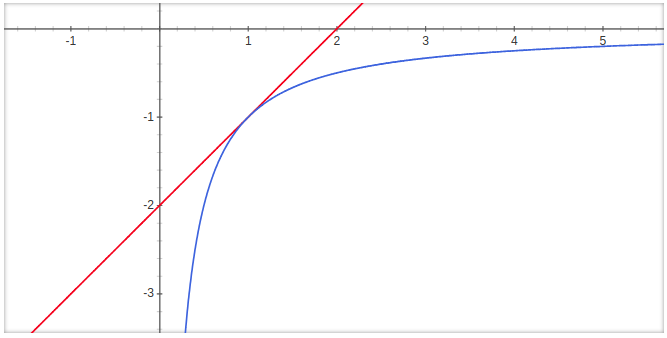
\includegraphics[width=0.49\textwidth]{derivata_00.png}\hfill%
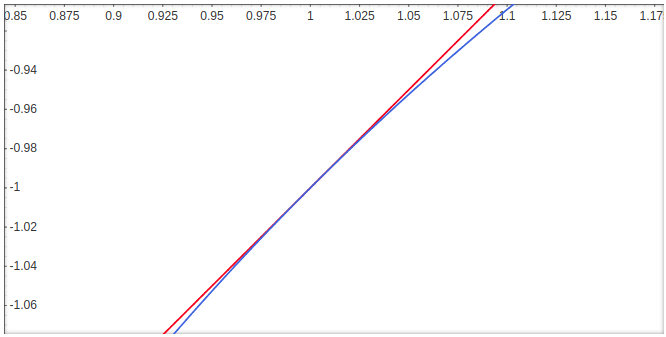
\includegraphics[width=0.49\textwidth]{derivata_01.png}
\label{fig:derivata}
\caption{Il grafico del potenziale gravitazionale terrestre.
Sull'asse delle $x$ la distanza dal centro della terra in raggi terrestri.
Sull'asse delle $y$ il potenziale gravitazionale con unità $C=GM/R$.
La pendenza della retta tangente al grafico della curva per $x=R$ è $g=GM/R^2$.
Nella figura di destra un ingrandimento in un intorno del raggio terrestre:
si nota come il grafico del potenziale risulta quasi indistinguibile dal
grafico della retta tangente.}
\end{figure}

Quello che abbiamo fatto è un procedimento di \emph{linearizzazione}%
\mymargin{linearizzazione}%
\index{linearizzazione}. 
Il campo gravitazionale è descritto da una funzione non lineare: $-GM/r$.
Ma quando ci restringiamo a un piccolo intervallo di valori di $r$ 
(i valori di $r$ vicini ad $R$, il raggio della terra) tale funzione 
risulta quasi indistinguibile, a meno di una costante, dalla funzione 
lineare $gh$ se $r=R+h$.
Le funzioni lineari sono molto più semplici da trattare ed è quindi conveniente, 
se rimaniamo sulla superficie terrestre, utilizzare quest'ultima formula per 
il potenziale gravitazionale.
Il grafico della funzione lineare che meglio approssima il grafico di una 
funzione si chiama \emph{retta tangente}%
\mymargin{retta tangente}%
\index{retta!tangente}. 
Il suo coefficiente angolare, $g$ nel nostro esempio, si chiama \emph{derivata}%
\mymargin{derivata}%
\index{derivata}.

Una volta introdotte le derivate vedremo che quello che abbiamo
determinato è la formula:
\[
U(R+h) = U(R) + U'(R) h + \omega(h).
\]

\begin{definition}[derivata]
\mymark{***}%
Sia $A\subset \RR$, $f\colon A \to \RR$, 
$x_0\in A$ un punto di accumulazione di $A$.
Diremo che la funzione $f$ è \emph{derivabile} nel punto $x_0$ se esiste
ed è finito il limite:
\[
  \lim_{h\to 0} \frac{f(x_0+h) - f(x_0)}{h}.
\]
In tal caso denoteremo con $f'(x_0)$ il valore di tale limite che chiameremo
\emph{derivata}%
\mymargin{derivata}%
\index{derivata} della funzione $f$ nel punto $x_0$.

Se $B$ è l'insieme dei punti di accumulazione di $A$ in cui $f$ risulta essere derivabile, risulta quindi definita la funzione derivata $f'\colon B \to \RR$.

Una funzione $f$ si dice essere derivabile se è derivabile in ogni punto del suo dominio.
Se $C\subset A$ la funzione $f$ si dice essere \emph{derivabile su $C$} se è derivabile in ogni punto dell'insieme $C$ (cioè se $C\subset B$).

Notazioni alternative per denotare la derivata di una funzione:
\[
  f' = Df = \frac{d}{dx} f = \frac{df}{dx}.
\]

La definizione di derivata si estende formalmente identica 
alle funzioni di variabile complessa e/o a valori complessi.
La derivata di una funzione a valori complessi è
a sua volta a valori complessi.
\end{definition}

Il rapporto
\[
\frac{f(x_0+h) - f(x_0)}{h}
\]
si chiama \emph{rapporto incrementale}%
\mymargin{rapporto incrementale}%
\index{rapporto!incrementale}. In effetti cambiando variabile e ponendo $x=x_0+h$ si può scrivere
\[
\frac{f(x_0+h) - f(x_0)}{h}
= \frac{f(x) - f(x_0)}{x-x_0}
= \frac{\Delta f}{\Delta x}
\]
che risulta essere il rapporto dell'incremento della funzione $f$ (a volte denotato con $\Delta f$) rispetto all'incremento corrispondente della variabile $x$ (a volte denotato con $\Delta x$).
Cambiando variabile nel limite, per $h\to 0$ si avrà $x\to x_0$
e quindi
\[
 f'(x_0) = \lim_{x\to x_0} \frac{f(x)-f(x_0)}{x-x_0}.
\]

Se $f$ è derivabile nel punto $x_0$
la retta di equazione 
\mymargin{retta tangente}%
\begin{equation}\label{eq:retta_tangente}
  y = f(x_0) + f'(x_0) \cdot (x-x_0)  
\end{equation}
è l'unica retta passante dal punto $(x_0,f(x_0))$ 
con pendenza uguale alla derivata $f'(x_0)$.
Tale retta si chiama \emph{retta tangente}
\index{retta!tangente}%
\index{tangente!al grafico}%
al grafico della funzione $f$ nel punto $(x_0,f(x_0))$.
E' la retta che meglio approssima il grafico di $f$ 
quando $x\to x_0$ nel senso che risulta:
\[
  \lim_{x\to x_0} \frac{f(x) - [f(x_0)+f'(x_0)(x-x_0)]}{x-x_0} = 0
\]
mentre ogni altra retta renderebbe questo limite infinito.

\begin{example}%
\label{ex:derivata_reciproco}%
\mymark{**}%
Si consideri la funzione $f(x) = 1/x$ definita sull'insieme $A = \RR \setminus \ENCLOSE{0}$. Si ha allora per ogni $x\neq 0$:
\[
  f'(x) = \lim_{h\to 0} \frac{\frac{1}{x+h} - \frac{1}{x}}{h}
        = \lim_{h\to 0} \frac{x - (x+h)}{h(x+h)x}
        = \lim_{h\to 0} \frac{-1}{(x+h)x} = -\frac{1}{x^2}.
\]
Risulta quindi che la funzione $1/x$ sia derivabile e la sua derivata è la funzione $-1/x^2$.
\end{example}

\begin{theorem}[continuità delle funzioni derivabili]
\mymark{***}
Se $f$ è derivabile nel punto $x$ allora $f$ è anche continua nel punto $x$.
\end{theorem}
%
\begin{proof}
\mymark{***}
Si ha
\[
  \lim_{h\to 0} f(x+h) - f(x) = \lim_{h\to 0} \frac{f(x+h) - f(x)}{h} \cdot h
  = f'(x) \cdot 0 = 0.
\]
Dunque $f(x+h)\to f(x)$ per $h\to 0$ e quindi $f$ è continua nel punto $x$.
\end{proof}

\begin{example}[funzione continua ma non derivabile]
\mymark{***}
La funzione $f(x) = \abs{x}$ è un esempio di funzione continua ma non
derivabile. E' infatti facile verificare che nel punto $x_0=0$ il
limite destro del rapporto incrementale è $1$ mentre il limite
sinistro è $-1$.

Un altro esempio è la funzione $f(x) = \sqrt{x}$ che è continua ma non
è derivabile nel punto $x_0=0$ perché il limite del rapporto incrementale esiste ma è $+\infty$.
\end{example}



\begin{theorem}[derivata della funzione composta]
\mymark{**}%
Sia $f$ una funzione derivabile nel punto $x_0$
e sia $g$ una funzione derivabile nel punto $f(x_0)$.
Allora la funzione composta $g\circ f$ è derivabile
nel punto $x_0$ e si ha:
\[
  (g\circ f)'(x_0) = g'(f(x_0))\cdot f'(x_0).
\]
\end{theorem}
%
\begin{proof}
\mymark{**}
Consideriamo la funzione
\[
  G(y) =
  \begin{cases}
   \frac{g(y) - g(f(x_0))}{y-f(x_0)} & \text{se $y \neq f(x_0)$},\\
   g'(f(x_0)) & \text{se $y=f(x_0)$}.
  \end{cases}
\]
Si avrà allora
\begin{equation}\label{eq:47439}
 \frac{g(f(x_0+h))-g(f(x_0))}{h}
 = G(f(x_0+h)) \cdot \frac{f(x_0+h)-f(x_0)}{h}
\end{equation}
infatti se $f(x_0+h)\neq f(x_0)$ abbiamo moltiplicato e diviso
per $f(x_0+h) - f(x_0)$ se invece $f(x_0+h)=f(x_0)$ allora anche $g(f(x_0+h))=g(f(x_0))$ e l'uguaglianza è ancora valida perché sia il lato sinistro che il lato destro si annullano (e il valore assegnato a $G$ risulta in tal caso irrilevante).

Chiaramente quando $h\to 0$ il secondo fattore sul lato destro
dell'uguaglianza \eqref{eq:47439}
tende, per definizione, a $f'(x_0)$.
Per quanto riguarda il primo fattore
osserviamo che $G(y)$, per come è stata definita, risulta essere una funzione continua nel punto $y=f(x_0)$ in quanto
\[
\frac{g(y) - g(f(x_0))}{y-f(x_0)} \to g'(f(x_0))
\]
per $y\to f(x_0)$.
Ma anche la funzione $f$ è continua nel punto $x_0$ (in quanto derivabile).
Dunque la funzione composta $G(f(x_0+h))$ è continua nel punto $h=0$.
Risulta quindi che $G(f(x_0+h)) \to G(f(x_0)) = g'(f(x_0))$ per $h\to 0$.
Dunque il lato destro di \eqref{eq:47439} ha limite $g'(f(x_0)) \cdot f'(x_0)$ per $h\to 0$, come volevamo dimostrare.
\end{proof}

\begin{theorem}[derivata della funzione inversa]
\mymark{**}
Sia $f$ una funzione invertibile derivabile in un punto $x_0$ e
supponiamo che la funzione inversa $f^{-1}$ sia continua in $f(x_0)$.
Se $f'(x_0)\neq 0$ allora $f^{-1}$ è derivabile in $f(x_0)$ e vale:
\[
  (f^{-1})'(f(x_0)) = \frac{1}{f'(x_0)}.
\]
Chiamato $y_0 = f(x_0)$ la formula può essere anche scritta nella forma:
\[
  (f^{-1})'(y_0) = \frac{1}{f'(f^{-1}(y_0))}.
\]
Se invece $f'(x_0)=0$ la funzione $f^{-1}$ non è derivabile in $f(x_0)$.
\end{theorem}
%
Osserviamo che 
se $I$ è un intervallo,
e se $f\colon I\to \RR$,
è iniettiva e continua allora $J=f(I)$ è un intervallo
e la funzione inversa $f^{-1}\colon J\to I$
è continua (Esercizio~\ref{ex:inversa_monotona}).
%
\begin{proof}
\mymark{**}
Posto $y_0 = f(x_0)$ consideriamo il rapporto incrementale di $f^{-1}$ nel punto $y_0$:
\[
  \frac{f^{-1}(y) - f^{-1}(y_0)}{y-y_0}.
\]
Per $y\to y_0$ possiamo fare il cambio di variabile
$x=f^{-1}(y)$ in quanto avendo assunto che $f^{-1}$ sia continua in $f(x_0)$ sappiamo che se $y\to y_0$ allora $x = f^{-1}(y)\to f^{-1}(y_0) = x_0$.
Si ha allora per $y\to y_0$ che $x\to x_0$ e,
se $f'(x_0)\neq 0$:
\[
  \frac{f^{-1}(y) - f^{-1}(y_0)}{y-y_0}
  = \frac{x-x_0}{f(x)-f(x_0)}
  = \frac{1}{\frac{f(x)-f(x_0)}{x-x_0}} \to \frac{1}{f'(x_0)}.
\]

Se invece $f'(x_0)=0$ il rapporto incrementale della funzione inversa
ha limite infinito e quindi la funzione inversa non è derivabile in $f(x_0)$.
\end{proof}


\begin{theorem}[operazioni con le derivate]
  \label{th:derivate_operazioni}%
\mymark{***}%
Siano $f$ e $g$ due funzioni derivabili in uno stesso punto $x_0$.
Allora le funzioni $f+g$, $f-g$, $f\cdot g$ e, se $g(x_0)\neq 0$ anche $f/g$ sono funzioni derivabili in $x_0$. Nei punti in cui entrambe le funzioni sono derivabili si ha
\begin{gather*}
  (f+g)' = f' + g', \qquad
  (f-g)' = f' - g', \\
  (f\cdot g)' = f' \cdot g + f g', \qquad
  \enclose{\frac{f}{g}}' = \frac{f'g - fg'}{g^2}.
\end{gather*}
\end{theorem}
%
\begin{proof}
\mymark{***}
Per quanto riguarda la derivata della somma (o della differenza) è sufficiente osservare che il rapporto incrementale della somma (o della differenza) è la somma (o la differenza) dei rapporti incrementali e che il limite della somma (o della differenza) è uguale alla somma (o la differenza) dei limiti.

Calcoliamo la derivata del prodotto $f\cdot g$ nel punto $x_0$. Si ha
\begin{align*}
  \frac{f(x)g(x) - f(x_0)g(x_0)}{x-x_0}
  &= \frac{f(x)(g(x) - g(x_0)) + (f(x)-f(x_0))g(x_0)}{x-x_0}\\
  &= f(x) \frac{g(x)-g(x_0)}{x-x_0} + \frac{f(x)-f(x_0)}{x-x_0} g(x_0).
\end{align*}
Passando al limite per $x\to x_0$ ci ricordiamo che $f(x)\to f(x_0)$ in quanto $f$ è continua in $x_0$ (essendo per ipotesi derivabile). I rapporti incrementali tendono alle derivate e si ottiene quindi il risultato voluto $f(x_0) g'(x_0) + f'(x_0) g(x_0)$.

Per quanto riguarda la derivata del rapporto osserviamo che
posto $h(y)=1/y$ si ha
\[
  \frac{f(x)}{g(x)} = f(x) \cdot h(g(x)).
\]
Dall'esempio~\ref{ex:derivata_reciproco} sappiamo che $h'(y) = -1/y^2$ e dunque
possiamo utilizzare le formule per la derivata del prodotto e la derivata della funzione composta per ottenere:
\begin{align*}
  \enclose{\frac{f}{g}}'(x_0)
  &= \enclose{f \cdot (g\circ h)}'(x_0) \\
  &= f'(x_0) \cdot h(g(x_0)) + f(x_0) \cdot h'(g(x_0))\cdot g'(x_0)\\
  &= \frac{f'(x_0)}{g(x_0)} + f(x_0) \cdot \frac{-1}{g^2(x_0)} g'(x_0)\\
  &= \frac{f'(x_0)g(x_0) - f(x_0)g'(x_0)}{g^2(x_0)}.
\end{align*}
\end{proof}

\begin{table}
  \begin{tabular}{c|c||c|c||c|c}
    $f(x)$ & $f'(x)$ & $f(x)$ & $f'(x)$ & $f(x)$ & $f'(x)$
    \\\hline
    $mx + q$ & $m$ &
    $e^x$ & $e^x$ &
    $\sin x$ & $\cos x$ \\
    $\abs{x}$ & $\frac{x}{\abs{x}}$ &
    $\ln x$ & $\frac 1 x$ &
    $\cos x$ & $-\sin x$ \\
    $x^n$ & $n x^{n-1}$ &
    $\sinh x$ & $\cosh x$ &
    $\arcsin x$ & $\frac{1}{\sqrt{1-x^2}}$ \\
    $x^\alpha$ & $\alpha x^{\alpha -1}$ &
    $\cosh x$ & $\sinh x$ & $\arccos x$ & $-\frac{1}{\sqrt{1-x^2}}$ \\
    $\sqrt[n]{x}$ & $\frac{1}{n\sqrt[n]{x^{n-1}}}$ &
    $\settsinh x$ & $\frac{1}{\sqrt{x^2+1}}$ &
    $\tg x$ & $1+ \tg^2 x$ \\
    $\sqrt{x}$ & $\frac{1}{2\sqrt{x}}$ &
    $\settcosh x$ & $\frac{1}{\sqrt{x^2-1}}$ &
    $\arctg x$ & $\frac{1}{1+x^2}$
  \end{tabular}
  \caption{Derivate delle funzioni elementari}
  \label{tab:derivate}%
\end{table}

\begin{theorem}[derivate delle funzioni elementari]%
\label{th:derivate_elementari}%
\index{derivata!delle funzioni elementari}%
\mymark{**}%
Per $m,q,\alpha \in \RR$, $\alpha \neq 0$, $n\in \NN$, $n\neq 0$
valgono le regole di derivazione riassunte nella
tabella~\ref{tab:derivate}: le funzioni nella colonna
$f(x)$ hanno la derivata riportata nella colonna $f'(x)$.
Le funzioni $f(x)$ sono derivabili nei punti del loro dominio 
in cui la corrispondente espressione $f'(x)$ è ben definita.
In particolare:
la funzione $\sqrt[n]{x}$
non è derivabile in $x=0$,
le funzioni $\arcsin x$ e $\arccos x$ non sono derivabili nei punti $-1$ e $1$,
la funzione $\abs{x}$ non è derivabile in $0$,
la funzione $\settcosh x$ non è derivabile in $1$,
la funzione $\ln x$ è derivabile per ogni $x>0$.
Le funzioni lineari, potenze con base positiva, potenze con esponente intero,
esponenziale, logaritmo, seno, coseno, tangente, arcotangente sono invece derivabili
in tutti i punti in cui sono definite.
\end{theorem}

\begin{proof}
\mymark{**}
Per quanto riguarda le funzioni lineari si ha:
\begin{align*}
(mx+q)' &= \lim_{h\to 0}\frac{m(x+h)+q - (mx+q)}{h} = \lim_{h\to 0} m = m.
\end{align*}
Ricordando che la derivata è un limite e che il limite in un punto dipende 
solo dai valori della funzione in un intorno del punto, 
possiamo affermare che la derivata del valore assoluto $\abs{x}$ 
coincide con la derivata di $x$ cioè $1$ sugli $x>0$ e coincide 
con la derivata di $-x$ sugli $x<0$. Dunque $D \abs{x} = x / \abs{x}$ 
se $x\neq 0$. 
Se $x=0$ i limiti destro e sinistro del rapporto incrementale di $\abs{x}$ 
tendono rispettivamente a $1$ e $-1$ e quindi la derivata non esiste.

Dimostriamo che $Dx^n = n x^{n-1}$ per $n\in \NN$, $n>0$, 
per induzione su $n$. Per $n=1$ abbiamo $x^n=x^1$ è lineare 
e quindi dalla formula precedente $Dx^1 = 1 = 1 \cdot x^0$. 
Supponendo di sapere che $D x^n = n x^{n-1}$ si ha, applicando 
la regola di derivazione del prodotto:
\[
  D x^{n+1} = D x\cdot x^n = 1 \cdot x^n + x \cdot n x^{n-1}
   = x^n + n x^n = (n+1) x^n
\]
dimostrando dunque il passo induttivo.
Ricordando la formula di derivazione del rapporto
possiamo trovare la formula per le potenze con esponente intero negativo:
\[
  D x^{-n} = D \frac{1}{x^n} = \frac{-n x^{n-1}}{x^{2n}}
   = -n x^{n-1-2n} = -n x^{-n-1}.
\]

La derivata della radice $n$-esima si trova con la formula di derivazione della funzione inversa $x^n$, che può essere applicata se $x\neq 0$:
\[
  D \sqrt[n]{x} = \frac{1}{n(\sqrt[n]{x})^{n-1}}
    = \frac{1}{n\sqrt[n]{x^{n-1}}}.
\]
Osserviamo che se $n$ è dispari la formula è valida anche per $x<0$.
La derivata della radice quadrata si ottiene ponendo $n=2$.

Per quanto riguarda la derivata dell'esponenziale
ci riconduciamo ad un limite notevole:
\[
  D e^x = \lim_{h\to 0} \frac{e^{x+h}-e^x}{h}
  = \lim_{h\to 0}\frac{e^x e^h - e^x}{h}
  = \lim_{h\to 0}e^x \frac{e^h - 1}{h}
  = e^x.
\]
La derivata del logaritmo si ottiene come derivata della funzione inversa dell'esponenziale:
\[
  D \ln x = \frac{1}{e^{\ln x}} = \frac{1}{x} \qquad\text{per $x>0$}.
\]
Possiamo quindi calcolare la derivata delle potenze con base positiva e esponente reale qualunque:
\[
D x^\alpha
= D e^{\alpha \ln x}
= e^{\alpha \ln x} D(\alpha \ln x)
= x^\alpha \alpha \frac{1}{x}
= \alpha x^{\alpha -1}.
\]

Per quanto riguarda le funzioni trigonometriche 
$\sin$ e $\cos$ ci ricordiamo del limite notevole
(teorema~\ref{th:limite_notevole_sin})
\[
  \lim_{h\to 0}\frac{\sin h}{h} = 1
\]
da cui si ricava, per $h\to 0$ 
\[
\frac{1-\cos h}{h}
= \frac{1-\cos^2 h}{h\cdot(1+\cos h)}
= \frac{\sin^2 h}{h\cdot (1+\cos h)}
= \frac{\sin h}{h} \cdot \frac{\sin h}{1+\cos h}
\to 1 \cdot \frac{0}{2} = 0.
\]
Applicando le formule di addizione si ha
\begin{align*}
  D \sin x
  &= \lim_{h\to 0}\frac{\sin(x+h)-\sin(x)}{h} \\
  &= \lim_{h\to 0}\frac{\sin(x)\cos(h) + \cos(x)\sin(h) - \sin(x)}{h} \\
  &= \lim_{h\to 0}\Enclose{\sin(x) \frac{\cos h-1}{h} + \cos(x) \frac{\sin h}{h}} 
  = \cos(x).
\end{align*}
e similmente
\begin{align*}
  D \cos x
  &= \lim_{h\to 0}\frac{\cos(x+h)-\cos(x)}{h} \\
  &= \lim_{h\to 0}\frac{\cos(x)\cos(h) - \sin(x)\sin(h) - \cos(x)}{h} \\
  &= \lim_{h\to 0}\cos(x) \frac{\cos h-1}{h} - \sin(x) \frac{\sin h}{h} = -\sin(x)
\end{align*}

La funzioni $\arcsin$ è definita come l'inversa della restrizione della funzione $\sin$ all'intervallo $[-\pi/2, \pi/2]$.
Nell'intervallo aperto $(-\pi/2,$ $\pi/2)$ la funzione $\sin$ ha derivata positiva e dunque risulta che la funzione inversa (che sappiamo essere continua) è derivabile in $(-1,1)$ e la sua derivata è
\[
D\arcsin x
= \frac{1}{\cos(\arcsin x)}
= \frac{1}{\sqrt{1-\sin^2 \arcsin x}}
= \frac{1}{\sqrt{1-x^2}}.
\]
Si ha infatti $\cos y = \sqrt{1-\sin^2 y}$ se $y\in [-\pi/2, \pi/2]$.

Analogamente la funzione $\arccos$ è definita come l'inversa della restrizione di $\cos$ all'intervallo $[0,\pi]$ e si ha quindi,
per $x\in (-1,1)$
\[
D \arccos x
 = \frac{1}{-\sin(\arccos x)}
 = \frac{1}{-\sqrt{1-\cos^2 \arccos x}}
 = -\frac{1}{\sqrt{1-x^2}}.
\]
Si ha infatti $\sin y = \sqrt{1-\cos^2 y}$ se $y\in[0,\pi]$.

Nei punti $x=1$ e $x=-1$ le funzioni $\arcsin$ e $\arccos$ non sono invece derivabili.

Per la funzione tangente possiamo utilizzare la formula di derivazione del rapporto:
\begin{align*}
  D \tg x &= D \frac{\sin x }{\cos x}
   = \frac{\cos x \cdot \cos x - \sin x \cdot (-\sin x)}{\cos^2 x} \\
   &= \frac{\cos^2 x + \sin^2 x}{\cos^2 x}
   = 1 + \tg^2 x = \frac{1}{\cos^2 x}.
\end{align*}
Usando la formula della derivata della funzione inversa si ha
\[
  D \arctg x = \frac{1}{1+\tg^2(\arctg x)}
  = \frac{1}{1+x^2}.
\]

Per quanto riguarda le funzioni iperboliche le derivate di $\sinh$
e $\cosh$ si riconducono immediatamente alla derivata dell'esponenziale,
utilizzando
la definizione~\eqref{eq:sinh_cosh}. Le derivate delle funzioni
inverse $\settsinh$ e $\settcosh$ si ottengono dalla formula per la derivata
della funzione inversa e utilizzando
le relazioni $\cosh x = \sqrt{\sinh^2 x+1}$ e, per $x > 0$,
$\sinh x = \sqrt{\cosh^2 x -1}$:
\begin{align*}
  D \settsinh x &= \frac{1}{\cosh(\settsinh x)}
  = \frac{1}{\sqrt{\sinh^2 (\settsinh x) + 1}} = \frac{1}{\sqrt{x^2+1}}\\
  D \settcosh x &= \frac{1}{\sinh(\settcosh x)}
  = \frac{1}{\sqrt{\cosh^2(\settcosh x)-1}}
  = \frac{1}{\sqrt{x^2-1}}
\end{align*}
\end{proof}

Si noti che le regole di derivazione appena dimostrate 
sono valide anche per le funzioni complesse $z^n$ e $e^z$:
in particolare si ha $D z^n = nz^{n-1}$ per ogni $n\in \ZZ$,
$n\neq 0$ e si ha $D e^z = e^z$ in quanto il limite 
notevole dell'esponenziale è valido anche in campo complesso.
Altre funzioni quali $\sqrt{x}$ 
oppure $\ln x$, non sono univocamente estendibili su $\CC$
e richiedono quindi una teoria a parte. 
Una volta definite, però, si potrebbe verificare 
che anche queste funzioni soddisfano le stesse regole di derivazione 
delle loro restrizioni reali.

\begin{proposition}[trucco di Feynman per le derivate]
  \index{trucco!di Feynman}%
  \index{trucco!di Feynman!per le derivate}%
  \index{Feynman!trucco per le derivate}%
Siano $f_1,\dots, f_n$ funzioni derivabili e siano $\alpha_1,\dots, \alpha_n$ 
esponenti reali. Allora:
  \[
  \enclose{\prod_{k=1}^n f_k^{\alpha_k}}'
  = \prod_{k=1}^n f_k^{\alpha_k} \cdot \sum_{k=1}^n \alpha_k \frac{f_k'}{f_k}.
  \]
\end{proposition}
\begin{proof}
Basta osservare che 
\begin{align*}
  \enclose{\prod_{k=1}^n f_k^{\alpha_k}}'
  &= \sum_{k=1}^n \alpha_k f_k' f_k^{\alpha_k-1} \prod_{j\neq k} f_j^{\alpha_j}
  = \sum_{k=1}^n \alpha_k \frac{f_k'}{f_k} \prod_{j=1}^n f_j^{\alpha_j}.
\end{align*}
\end{proof}
Se ad esempio vogliamo calcolare la derivata della funzione 
\[
 f(x) = \frac{\sqrt{1-x^2}\cdot \ln x}{x\cdot \cos^2 x}
 = (1-x^2)^{\frac 1 2} \cdot \ln x \cdot x^{-1}\cdot (\cos x)^{-2}
\]
otteniamo 
\begin{align*}
  f'(x) 
  &= \frac{\sqrt{1-x^2}\cdot \ln x}{x\cdot \cos^2 x}
  \cdot \Enclose{\frac 1 2 \cdot \frac{-2x}{1-x^2} + \frac{1}{x\ln x} - \frac{1}{x}-2\frac{-\sin x}{\cos x}}\\
  &=\frac{\sqrt{1-x^2}\cdot \ln x}{x\cdot \cos^2 x}
  \cdot \Enclose{-\frac{x}{1-x^2} + \frac{1}{x\ln x} - \frac{1}{x}+2\tg x}.
\end{align*}


\section{derivate parziali}

Capita a volte di avere funzioni che dipendono da più variabili o da parametri.
Ad esempio la funzione $f(x,y) = x^2y+y^2$ è una funzione definita 
sulle coppie di numeri reali: $f\colon \RR^2\to \RR$.
Se considero una delle due variabili, ad esempio la prima variabile $x$, 
come un parametro fissato, posso identificare la funzione $f$ con 
una funzione $g\colon \RR \to (\RR^\RR)$ 
che ad ogni valore del parametro $x$ restituisce una funzione 
della variabile $y$:
\[
  g(x)(y) = f(x,y).
\]
Dunque per ogni $x$ fissato, posso considerare la funzione $h=g(x)$
che è una funzione della sola variabile $y$: $h(y) = g(x)(y) = f(x,y)$.  
E posso quindi farne la derivata $h'(y)$ in qualunque punto $y$. 
Il valore che ottengo si chiama \emph{derivata parziale}%
\mymargin{derivata parziale}%
\index{derivata!parziale}
della funzione $f$ rispetto alla variabile $y$ calcolata nel punto $(x,y)$.
Per fare il calcolo della derivata possiamo applicare le usuali regole di 
derivazione facendo attenzione che se stiamo 
facendo la derivata rispetto a $y$ la variabile $x$ va trattata come se 
fosse costante, perché stiamo in effetti fissando $x$ prima di fare la derivata.
Se $f(x,y) = x^2y+y^2$ si ottiene dunque%
\mynote{Se non siamo abituati a pensare che $x$ possa essere un valore fissato 
si provi a sostituire la variabile $x$ con una lettera diversa come $c$ o $\pi$ che ci dà l'idea 
di una quantità costante.}:
$h'(y) = x^2 + 2y$.
Se ora consideriamo anche $x$ variabile otteniamo una nuova funzione di due 
variabili $(x,y)\mapsto (g(x))'(y) = h'(y)$ che può essere scritta 
con le seguenti notazioni% 
\mynote{%
Si osservi che per le funzioni di più variabili c'è una ambiguità di fondo nelle notazioni.
Infatti se ho una espressione in due variabili come $x^2 y + y^2$ è chiaro 
che questa rappresenta una funzione di due variabili ma non è del tutto ovvio dire quale 
è la prima variabile e quale è la seconda. 
Normalmente le variabili vengono indicate in ordine alfabetico a partire dalla $x$... 
ma è solo una convenzione. In principio l'espressione $x^2y + y^2$ 
potrebbe anche rappresentare una funzione di tre variabili $x,y,z$. 
Dunque se ho una espressione che utilizza certi nomi per le variabili è naturale 
usare gli stessi nomi nel simbolo utilizzato per la derivata parziale come 
nella notazione $D_y$.
Se invece le variabili non hanno un nome sarebbe più sensato indicare la variabile dandone 
la posizione numerica come nella notazione $D_2$.
Ci sono casi in cui la notazione può essere molto ambigua, come ad esempio 
se scrivessi $\frac{\partial f(y,x)}{\partial y}$: 
sto derivando $f$ rispetto alla prima variabile oppure derivo $f(x,y)$ rispetto alla seconda 
variabile e poi scambio le due variabili?
}:
\begin{align*}
\frac{\partial f(x,y)}{\partial y} 
&= \frac{\partial f}{\partial y}(x,y)
= D_y f(x,y)
= f_y (x,y) \\
&= D_2 f(x,y) = f_{,2} (x,y) \\
&= h'(y)
\end{align*}

Analogamente potremmo fare la derivata parziale di $f$ rispetto alla prima 
variabile $x$. Se $f(x,y) = x^2y+y^2$ si ottiene
\[
\frac{\partial f(x,y)}{\partial x} = 2xy.
\]

Stiamo qui trattando le funzioni di più variabili come se fossero funzioni di una sola 
variabile dipendenti da altri parametri. 
Questo perché stiamo facendo un corso di analisi sulle funzioni di \emph{una} variabile (reale).
\index{una!variabile}%
\index{funzione!di una variabile}%
\index{variabile!funzione di una}%
Per trattare tutte le variabili come una unica variabile multidimensionale 
bisogna fare diverse considerazioni 
aggiuntive che vengono trattate nei corsi di analisi sulle funzioni di 
\emph{più} 
\index{più!variabili}%
\index{funzione!di più variabili}%
\index{variabili!funzione di più}%
variabili (reali). 
Verranno in tal caso introdotti i concetti di \emph{gradiente} $\nabla f$, 
\emph{derivata} $Df$ e \emph{differenziale} $df$ che noi non affronteremo qui.


\section{punti notevoli}

In questa sezione introdurremo una terminologia che è largamente utilizzata 
nello studio di funzione.
Cercheremo di dare delle definizioni anche per alcuni termini su cui potrebbe 
non esserci un consenso univoco.
Ricordiamoci di non usare queste definizioni in modo troppo formale:
sarà sempre meglio
verificare che il nostro interlocutore ci comprenda
perché spesso alcuni termini potrebbero essere utilizzati in maniera
impropria o con significati leggermente diversi.

Nel dubbio potremo sempre evitare di utilizzare questa terminologia 
riconducendoci ai concetti sottostanti.

\begin{definition}[punti notevoli]
Sia $f\colon A \subset \RR \to \RR$ una funzione. Se $f$ è derivabile in un
punto $x_0\in A$ e $f'(x_0) = 0$ diremo che $x_0$ è un \emph{punto critico}%
\mymargin{punto critico}%
\index{punto!critico}
o
\emph{punto stazionario}
\index{punto!stazionario}
di $f$.

Se $x_0\in A$ ed esiste un intorno $U$ di $x_0$ per cui $x_0$ risulta
essere un punto di minimo (rispettivamente di massimo) per $f$ ristretta ad $U$
diremo che $x_0$ è un punto di \emph{minimo relativo}%
\mymargin{minimo relativo}%
\index{minimo!relativo} o \emph{minimo locale}
(rispettivamente \emph{massimo relativo} o \emph{massimo locale}).
Per contrapposizione i punti di massimo e minimo su tutto il dominio $A$
vengono anche
chiamati massimo/minimo \emph{assoluto} di $f$.

Diremo che $x_0\in A$ è un \emph{punto di flesso}%
\mymargin{punto di flesso}%
\index{punto!di flesso} per $f$ se
$f$ è derivabile in un intorno di $x_0$ e $x_0$ è un punto di massimo
o minimo relativo per $f'$. Nel punto $x_0$ la retta tangente
ha equazione $y=r(x) = f'(x_0) (x-x_0) + f(x_0)$. Se $x_0$ è
minimo per $f'$ risulta che $f(x)-r(x)$ è crescente
quindi $f(x)\ge r(x)$ per $x\ge x_0$ e $f(x)\le r(x)$ per $x\le x_0$
(il grafico della funzione attraversa la retta tangente da sotto a sopra)
mentre se $x_0$ è massimo per $f'$ risulta che $f(x)\le r(x)$ per $x\ge x_0$
e $f(x) \ge r(x)$ per $x\le x_0$ (il grafico della funzione attraversa
la tangente da sopra a sotto).
Se la funzione $f$ non è derivabile in $x_0$ ma il limite del rapporto
incrementale esiste ed è infinito, diremo che $x_0$ è un
\emph{flesso verticale}%
\mymargin{flesso verticale}%
\index{flesso!verticale}. In tale punto la retta tangente è verticale
e il grafico della funzione attraversa tale retta.

Sia $x_0\in A$ un punto in cui la funzione $f$ è continua ed esistono
i limiti destro e sinistro del rapporto incrementale
(che si chiamano \emph{derivata destra} e \emph{derivata sinistra})
\[
  m^{\pm} = \lim_{h\to 0^\pm}\frac{f(x+h) - f(x)}{h}.
\]
Se $m^+ \neq m^-$ chiaramente $f$ non è derivabile in $x_0$.
Se entrambi $m^+$ ed $m^-$ sono finiti diremo che $x_0$ è un
\emph{punto angoloso}%
\mymargin{punto angoloso}%
\index{punto!angoloso} in quanto le due semirette tangenti
in $x_0$ (da destra e da sinistra) formano un angolo non piatto.
Se $m^+=-m^-=+\infty$ oppure se $m^+=-m^-=-\infty$
diremo che il punto $x_0$ è un \emph{punto di cuspide}%
\mymargin{punto di cuspide}%
\index{punto!di cuspide} (c'è una
semiretta tangente verticale).
\end{definition}

\begin{definition}[asintoti]
Diremo che la retta $y=mx+q$ è un asintoto per il grafico di $f$ 
per $x\to +\infty$ se risulta
\[
  \lim_{x\to +\infty} f(x) - (mx+q) = 0.
\]
Se $m=0$ diremo che il grafico di $f$ ha un \emph{asintoto orizzontale} $y=q$
\mymargin{asintoto orizzontale e obliquo}%
\index{asintoto orizzontale e obliquo}%
\index{asintoto!orizzontale}%
\index{asintoto!obliquo}%
altrimenti diremo che $y=mx+q$ è un \emph{asintoto obliquo}.
Stessa cosa si può dire per $x\to -\infty$.

Se $x_0\in \RR$ e si ha 
\[
  \lim_{x\to x_0} \abs{f(x)} = +\infty
\]
diremo che la retta $x=x_0$ è un \emph{asintoto verticale}%
\mymargin{asintoto verticale}%
\index{asintoto!verticale} per il 
grafico della funzione $f$.
\end{definition}

\begin{definition}[punti di discontinuità]
Se per $x_0\in \RR$ si ha 
\[
  \lim_{x\to x_0^-} f(x) = \ell_1, 
  \qquad 
  \lim_{x\to x_0^+} f(x) = \ell_2
\]
e se $\ell_1\neq \ell_2$ diremo che nel punto $x_0$ 
la funzione $f$ ha una \emph{discontinuità a salto}%
\mymargin{discontinuità a salto}%
\index{discontinuità!a salto}.
Se $\ell_1=\ell_2$ e se $f$ non è definita nel punto $x_0$ 
oppure se $f(x_0)\neq \ell_1$ diremo che 
nel punto $x_0$ la funzione $f$ 
ha una \emph{discontinuità eliminabile}%
\mymargin{discontinuità eliminabile}%
\index{discontinuità!eliminabile}.
\end{definition}

Si osservi che, nonostante la terminologia utilizzata,
una funzione continua può avere una discontinuità 
a salto (ad esempio: $f(x)=\frac{x}{\abs{x}}$) 
e può anche avere una discontinuità eliminabile
(ad esempio: $f(x) = \frac{x}{x}$).


\section{il teorema di Lagrange e criteri di monotonia}

\begin{theorem}[Fermat]
\mymark{***}
Sia $f\colon (a,b)\to \RR$ una funzione derivabile.
Se $x_0\in (a,b)$ è un punto di massimo o minimo per $f$ allora
$f'(x_0)=0$.
\end{theorem}
%
\begin{proof}
\mymark{***}
Senza perdere di generalità possiamo suppore che $x_0$ sia un punto di massimo per $f$.
Sappiamo che
\[
  f'(x_0) = \lim_{x\to x_0}\frac{f(x)-f(x_0)}{x-x_0}.
\]
Visto che $x_0$ è un punto dell'intervallo aperto $(a,b)$ la funzione $f$ è definita in un intorno destro di $x_0$ e quindi possiamo restingere il limite ai valori $x>x_0$ ottenendo:
\[
  f'(x_0) = \lim_{x\to x_0^+}\frac{f(x) - f(x_0)}{x-x_0}.
\]
Visto che $x_0$ è un punto di massimo per $f$ sappiamo che $f(x)-f(x_0)\le 0$. Essendo $x-x_0>0$ l'intero rapporto incrementale risulta essere non positivo.
Dunque, per il teorema della permanenza del segno,
possiamo concludere che $f'(x_0)\le 0$.

Ma possiamo anche restringere la funzione ad un intorno sinistro di $x_0$ e osservare che
\[
  f'(x_0) = \lim_{x\to x_0^-}\frac{f(x)-f(x_0)}{x-x_0}.
\]
Ma ora il numeratore è, come prima, non positivo mentre il denominatore $x-x_0$ è negativo. Dunque il rapporto incrementale stavolta è non negativo e quindi, per la permanenza del segno, $f'(x_0) \ge 0$.

Abbiamo scoperto quindi che $f'(x_0)\le 0$ e $f'(x_0)\ge 0$
da cui deduciamo $f'(x_0)=0$.
\end{proof}

Il teorema di Fermat si può
enunciare dicendo che ogni punto di massimo o minimo relativo interno
al dominio di una funzione in cui la funzione è derivabile
è necessariamente un punto critico.
In particolare per determinare massimi e minimi assoluti e relativi
di una funzione sarà sufficiente esaminare i punti di frontiera,
i punti di non derivabilità e i punti critici.

\begin{exercise}[derivazione della legge di Snell dal principio di Fermat]
  \label{ex:snell}
  \index{legge!di Snell}%
  \index{Snell!legge di}%
  \index{principio!di Fermat}%
  \index{Fermat!principio di}%
Vogliamo quantificare il fenomeno di rifrazione
per cui un raggio luminoso viene deviato nel punto in cui 
il raggio attraversa la superficie di separazione 
tra due mezzi con indici di rifrazione diversi. 
Ad esempio un raggio che attraversa una lente di vetro passa 
prima dall'aria al vetro e poi dal vetro all'aria:
in questi passaggi il raggio viene deviato, permettendo di fatto di 
utilizzare le lenti per focalizzare la luce.

\begin{figure}
  \begin{center}
\begin{tikzpicture}[scale=1.5]
    % Surface (parabolic for illustration)
    \fill[blue!10] (-3,-1.2) -- (3,-1.2) -- plot[domain=3:-3] (\x, {-0.05*\x*\x}) -- cycle;
    \draw[thick, blue, domain=-3:3] plot (\x, {-0.05*\x*\x});
    \node at (-1.8,-0.3) { \( y = u(x) \) };

    % Axes
    \draw[->] (-3,0) -- (3,0) node[below left]{$x$};
    \draw[->] (0,-1.2) -- (0,1.5) node[below right]{$y$};
    
    
    % Point O
    \fill (0,0) circle (1pt) node[below left]{$O$};
    
    % Incident ray
    \draw[thick] (-1,1.5) -- (0,0);
    \fill (-1,1.5) circle (1pt) node[left]{$P_1$};
    
    % Refracted ray
    \draw[thick] (0,0) -- (1.5,-1);
    \fill (1.5,-1) circle (1pt) node[right]{$P_2$};
    
    % Variation ray
    \draw[dashed] (-1,1.5) -- (0.3,{-0.05*0.3*0.3}) -- (1.5,-1);
    \fill (0.3,{-0.05*0.3*0.3}) circle (1pt) node[above right]{$(x,u(x))$};

    % angles
    \draw (0,0.3) arc (90:123.69:0.3) node[left]{$\theta_1$};
    \draw (0,-0.3) arc (-90:-33.69:0.3) node[midway, below right]{$\theta_2$};
\end{tikzpicture}  \end{center}
\caption{Principio di Fermat, vedi esercizio~\ref{ex:snell} sulla derivazione della legge di Snell.}
\end{figure}

Si ipotizza che tra due punti sufficientemente vicini lungo il percorso 
del raggio luminoso la luce percorra il tragitto che minimizza il tempo di percorrenza.%
\footnote{
  Questo principio è noto come principio di Fermat 
  ed è la prima formulazione del principio di minima azione in fisica.
  Nella fisica moderna si sostituisce la richiesta di avere un minimo con quella 
  di avere un punto stazionario.
  Quindi si prende come principio la tesi del teorema di Fermat 
  invece che l'ipotesi.
  }
Si ipotizza inoltre che la velocità della luce sia costante all'interno di ciascun mezzo
(ma diversa nei due mezzi).

Consideriamo il punto $O$ in cui la luce passa da un mezzo all'altro
e consideriamo il piano contenente i due raggi incidenti e rifratti nel 
punto $O$. Su questo piano mettiamo un sistema di assi cartesiani 
con la $x$ orientata lungo il piano tangente in $O$ alla superificie 
di separazione tra i due mezzi e con l'asse $y$ perpendicolare 
a tale superficie. 
Siano $(x_1,y_1)$ e $(x_2,y_2)$ le coordinate di due punti qualunque $P_1$ e $P_2$, 
il primo sul raggio di incidenza e il secondo sul raggio rifratto, diversi da $O$
e sufficientemente vicini ad $O$ per poter ipotizzare che il percorso 
più breve da $P_1$ a $P_2$ sia quello che percorre prima il segmento 
da $P_1$ a $O$ e poi il segmento da $O$ a $P_2$.

L'angolo di incidenza $\theta_1$ e l'angolo di rifrazione $\theta_2$
sono quindi dati dalle seguenti formule:
\[
  \sin \theta_1 = -\frac{x_1}{\sqrt{x_1^2+y_1^2}},\qquad
  \sin \theta_2 = \frac{x_2}{\sqrt{x_2^2+y_2^2}}.
\]

Sia $u(x)$ la funzione che descrive il profilo della superificie 
di separazione tra i due mezzi. Per come abbiamo scelto il sistema di 
coordinate sia ha $u(0)=0$ e $u'(0)=0$. 
%Supponiamo che $u$ sia di classe $C^1$.
Possiamo allora scrivere la funzione $f(x)$ che rappresenta
il tempo di percorrenza di un raggio luminoso che percorre 
il segmento da $(x_1,y_1)$ a $(x,u(x))$ nel primo mezzo e poi 
il segmento da $(x,u(x))$ a $(x_2,y_2)$ nel secondo mezzo.
Se $c_1$ e $c_2$ sono le velocità della luce nei due mezzi 
si avrà:
\[
  f(x) = \frac{1}{c_1} \sqrt{(x - x_1)^2 + (u(x) - y_1)^2} +
         \frac{1}{c_2} \sqrt{(x - x_2)^2 + (u(x) - y_2)^2}.
\]
Per ipotesi la funzione $f$ assume un minimo in $x=0$ 
e dunque, per il teorema di Fermat, si deve avere $f'(0)=0$.
Calcoliamo quindi la derivata di $f$ 
\[
  f'(x) = \frac{1}{c_1}\frac{x - x_1 + (u(x)-y_1)u'(x)}{\sqrt{(x-x_1)^2 + (u(x)-y_1)^2}} +
          \frac{1}{c_2}\frac{x - x_2 + (u(x)-y_2)u'(x)}{\sqrt{(x-x_2)^2 + (u(x)-y_2)^2}}
\]
e la valutiamo in $x=0$, 
ricordando che $u(0)=0$ e $u'(0)=0$:
\[
  f'(0) = \frac{1}{c_1}\frac{- x_1}{\sqrt{x_1^2 + y_1^2}} +
          \frac{1}{c_2}\frac{- x_2}{\sqrt{x_2^2 + y_2^2}}
        = \frac{\sin \theta_1}{c_1} - \frac{\sin \theta_2}{c_2}.
\]
La condizione $f'(0)=0$ ci dà la legge di Snell:
\[
  \frac{\sin \theta_1}{c_1} = \frac{\sin \theta_2}{c_2}.
\]
\end{exercise}

\begin{theorem}[Rolle]
\mymark{***}
\index{teorema!di Rolle}
\mymargin{Rolle}%
\index{Rolle}
Sia $f\colon [a,b]\to \RR$, $a,b\in \RR$, $a<b$, una funzione continua su tutto $[a,b]$ e derivabile su $(a,b)$.
\mynote{Se $b<a$ il teorema è ugualmente valido 
se si intende $[a,b]=[b,a]$}%
Se $f(a) = f(b)$ allora esiste $x_0 \in (a,b)$ tale che $f'(x_0)=0$.
\end{theorem}
%
\begin{proof}
\mymark{***}
Essendo $f$ una funzione continua
possiamo applicare il teorema di Weiestrass per dedurre che $f$ ha massimo e 
minimo sull'intervallo chiuso e limitato $[a,b]$. 
Se il punto di massimo o il punto di minimo sta nell'intervallo aperto 
$(a,b)$ possiamo applicare il teorema di Fermat per ottenere che la derivata 
di $f$ si annulla in tale punto.

In caso contrario sia il punto di massimo che il punto di minimo sono estremi 
dell'intervallo, cioè sono uguali ad $a$ o a $b$. Ma visto che $f(a)=f(b)$ 
i valori massimo e minimo coincidono e quindi la funzione è costante. 
Ma in tal caso $f'(x)=0$ per ogni $x\in [a,b]$.
\end{proof}

\begin{theorem}[Lagrange]\label{th:lagrange}%
\mymark{***}%
\index{teorema!di Lagrange}%
\mymargin{Lagrange}%
\index{Lagrange}%
Sia $f\colon [a,b]\to \RR$ una funzione continua su $[a,b]$ e derivabile su $(a,b)$
con $a,b\in \RR$, $a<b$.
\mynote{Se $b<a$ il teorema è ugualmente valido 
se si intende $[a,b]=[b,a]$}%
Allora esiste un punto $x_0\in (a,b)$ tale che
\[
  f'(x_0) = \frac{f(b) - f(a)}{b-a}
\]
\end{theorem}
%
\begin{proof}
\mymark{***}
Consideriamo la funzione ausiliaria:
\[
  g(x) = f(x) - \frac{f(b)-f(a)}{b-a} x.
\]
Per verifica diretta si osserva che
\[
  g(b) = g(a) = \frac{b f(a) - a f(b)}{b-a}.
\]
La funzione $g$ soddisfa quindi le ipotesi del teorema di Rolle e dunque esisterà $x_0\in (a,b)$ tale che $g'(x_0)=0$.
Ma si osserva che
\[
  g'(x) = f'(x) - \frac{f(b)-f(a)}{b-a}
\]
e dunque se $g'(x_0)=0$ si ottiene il risultato desiderato.
\end{proof}

\begin{theorem}[criteri di monotonia]%
\label{th:criteri_monotonia}
\mymark{***}%
\mymargin{criteri di monotonia}%
\index{criterio!di monotonia}%
Sia $f\colon I \to \RR$ una funzione definita su un intervallo $I\subset \RR$. Sia $J= (\inf I, \sup I)$ l'intervallo aperto con gli stessi estremi di $I$.
Supponiamo che $f$ sia continua su $I$ e derivabile su $J$. 
Allora valgono i seguenti criteri:
\begin{enumerate}
\item
$(\forall x \in J\colon f'(x)\ge 0)$
$\iff$
$f$ è crescente (su tutto $I$);
\item
$(\forall x \in J\colon f'(x)\le 0)$
$\iff$
$f$ è decrescente (su tutto $I$);
\item
$(\forall x \in J\colon f'(x)=0)$
$\iff$
$f$ è costante (su tutto $I$);
\item
$(\forall x \in J\colon f'(x)>0)$
$\implies$
$f$ è strettamente crescente (su tutto $I$);
\item
$(\forall x \in J\colon f'(x)<0)$
$\implies$
$f$ è strettamente decrescente (su tutto $I$).
\end{enumerate}
\end{theorem}
%
\begin{proof}
\mymark{***}
Dimostriamo innanzitutto le implicazioni da sinistra verso destra.

Per la prima, se $f$ non fosse crescente ci dovrebbero essere due punti $a, b \in I$ tali che $a < b$ ma $f(a) > f(b)$.
Dunque si avrebbe
\[
  \frac{f(b) - f(a)}{b - a} < 0.
\]
Applicando il teorema di Lagrange all'intervallo $[a,b]$ si troverebbe un punto $x\in (a,b)$ tale che $f'(x) < 0$. Chiaramente $(a,b)\subset J$ e quindi questo contraddice l'ipotesi $f'(x) \ge 0$.

La seconda implicazione (per le funzioni decrescenti) si dimostra in maniera analoga cambiando verso alle disuguaglianze.

Anche la terza implicazione si dimostra tramite il teorema di Lagrange in modo analogo alle precedenti. Oppure basta osservare che se $f'(x)=0$ allora valgono contemporaneamente $f'(x)\ge 0$ e $f'(x)\le 0$ quindi mettendo insieme le prime due implicazioni si ottiene che $f$ è contemporaneamente crescente e decrescente dunque è costante.

Per la quarta implicazione si procede come per la prima. Per assurdo si  avrebbero $a<b$ con $f(b) \le f(a)$. Ma allora
\[
  \frac{f(b) - f(a)}{b-a} \le 0
\]
e applicando il teorema di Lagrange si troverebbe un punto $x\in (a,b)$ con $f'(x) \le 0$, contro l'ipotesi $f'(x) > 0$.

La quinta implicazione si dimostra in maniera analoga cambiando verso alle disuguaglianze.

Vediamo ora le implicazioni da destra verso sinistra.
Per la prima, supponiamo che $f$ sia crescente e prendiamo $x\in J$. Allora è chiaro che per ogni $h>0$ si avrà $f(x+h) \ge f(x)$ e dunque
\[
  \frac{f(x+h)- f(x)}{h} \ge 0.
\]
Facendo il limite per $h \to 0^+$ si ottiene $f'(x)$ e, per la permanenza del segno, dovra essere $f'(x) \ge 0$.

In maniera analoga (invertendo le disuguaglianze) si dimostra la seconda implicazione.

La terza discende dalle prime due oppure, più semplicemente, dalle regole di derivazione, in quanto la derivata di una costante è zero.
\end{proof}

\begin{example}
La funzione $f(x) = 1/x$ è definita su $\RR \setminus \ENCLOSE{0}$, è derivabile
e la derivata $f'(x) = -1/x^2$ è ovunque negativa. La funzione $f$ è quindi strettamente
decrescente separatamente sui due intervalli $(0,+\infty)$ e $(-\infty,0)$ sui quali
possiamo applicare il criterio di monotonia. Ma non è
decrescente su tutto il suo dominio in quanto, ad esempio, $f(-1) = -1 < 1 = f(1)$.
Questo esempio mostra che nei criteri di monotonia l'ipotesi che il dominio sia un intervallo
è fondamentale.
\end{example}

\begin{exercise}[estensione continua]
  \label{ex:estensione_continua_derivata_limitata}
Sia $f\colon (a,b)\to \RR$ una funzione derivabile con derivata 
limitata: $\abs{f'(x)} \le L$ per ogni $x\in (a,b)$.
Allora esiste il limite di $f(x)$ per $x\to a^+$ e per $x\to b^-$.
E se $f$ è anch'essa limitata tali limiti sono finiti, dunque 
$f$ si estende in modo continuo a tutto $[a,b]$.
\end{exercise}
\begin{proof}
Se il limite per $x\to a^+$ di $f$ non esistesse allora,
per il teorema~\ref{th:ponte} di collegamento tra limite di funzione 
e limite di successione, esisterebbero due successioni $a_n, b_n \to a^+$
tali che $\lim f(a_n) \neq \lim f(b_n)$
(ad esempio $f(a_n)\to \limsup_{x\to a^+} f(x)$ e
$f(b_n)\to \liminf_{x\to a^+} f(x)$).
Ma per il teorema di Lagrange, per ogni $n$ esisterebbe $c_n \in (a_n, b_n)$ tale che
\[
  \abs{f'(c_n)} =
  \abs{\frac{f(b_n) - f(a_n)}{b_n - a_n}}
\]
e visto che $f(b_n)-f(a_n)$ non tende a zero mentre $b_n - a_n \to 0$
si avrebbe che $\abs{f'(c_n)} \to +\infty$,
contraddicendo l'ipotesi che la derivata sia limitata.
Dunque il limite per $x\to a^+$ di $f$ esiste e analogamente si dimostra che esiste
il limite per $x\to b^-$ di $f$.

Se inoltre $f$ è limitata
allora i limiti trovati sono finiti e 
dunque $f$ si estende in modo continuo ad un funzione $\tilde f\colon [a,b]\to \RR$ 
definita come
\[
  \tilde f(x) = \begin{cases}
    f(x) & \text{se }x\in (a,b),\\
    \displaystyle\lim_{x\to a^+} f(x) & \text{se } x=a,\\
    \displaystyle\lim_{x\to b^-} f(x) & \text{se } x=b.
  \end{cases}
\]
\end{proof}

\section{studio di funzione}

\begin{exercise}
\index{problema!della lattina}%
\index{lattina!problema della}%
Determinare raggio e altezza di una lattina cilindrica di volume $33 cl$
che a parità di volume ha la minima superficie totale.
\end{exercise}
\begin{proof}[Svolgimento.]
Sia $V$ il volume, $S$ l'area della superficie totale, $h$ l'altezza e $r$
il raggio di base del cilindro.
Sappiamo che
\[
  V = \pi h r^2, \qquad
  S = 2\pi r h + 2 \pi r^2.
\]
Ricavando $h$ dalla prima equazione e sostituendo nella seconda otteniamo
\[
  S = 2 \pi r \frac{V}{\pi r^2} + 2 \pi r^2
    = \frac{2V}{r} + 2 \pi r^2.
\]
La funzione $S(r)$ è definita e continua su $(0,+\infty)$
e si ha $S(r)\to +\infty$ per $r\to 0^+$
e anche per $r\to +\infty$. 
Dunque $S$ ammette minimo per il teorema di Weierstrass
generalizzato.
Per trovare il minimo basterà calcolare la derivata
\[
 \frac{dS}{dr} = -\frac{2V}{r^2} + 4 \pi r = \frac{4\pi r^3 - 2V}{r^2}
\]
e trovare i punti critici
\[
  4\pi r^3 = 2V
\]
da cui
\begin{align*}
 r = \sqrt[3]{\frac{V}{2\pi}} \approx 3.74 cm\\
 h = \frac{V}{\pi r^2} \approx 7.49 cm.
\end{align*}
\end{proof}

\begin{exercise}
Risolvere l'equazione
\begin{equation} \label{eq:4734521}
  e^x = x^3.
\end{equation}
\end{exercise}
%
\begin{proof}[Svolgimento.]
Il lato sinistro dell'equazione è un numero positivo e quindi
certamente possiamo supporre che sia $x>0$ altrimenti il lato destro non sarebbe anch'esso positivo.
Possiamo quindi prendere il logaritmo di ambo i membri
e ottenere l'equazione
\[
  x = 3 \ln x
\]
che è equivalente all'equazione data.

Consideriamo allora la funzione
\[
 f(x) = x - 3 \ln x
\]
cosicché le soluzioni cercate risultano essere gli zeri di $f$.
Si ha
\[
  f'(x) = 1 - \frac{3}{x}
\]
e possiamo quindi affermare che
\mynote{Il simbolo $\gtrless$ serve per indicare che questa
diseguazione e le seguenti possono essere scritte sia con il segno
$>$ che con il segno $<$ pur di prendere in tutte lo stesso segno.}%
$f'(x) \gtrless 0$
se e solo se
\[
  1 \gtrless \frac 3 x
\]
ovvero (ricordiamo che stiamo supponendo $x>0$)
\[
  x \gtrless 3.
\]
Cioè: se $x>3$ si ha $f'(x)>0$ e di conseguenza
(teorema~\ref{th:criteri_monotonia})
$f$ è strettamente crescente se ristretta all'intervallo
$[3,+\infty)$,
se invece $x<3$ si ha $f'(x)<0$ e di conseguenza
$f$ è strettamente decrescente se ristretta all'intervallo
$(0,3]$.
Per capire se la funzione $f$ si annulla in qualche punto
dobbiamo ora valutare $f$ negli estremi degli intervalli su cui risulta monotona. Si ha
\[
  \lim_{x\to 0^+} f(x) = +\infty, \qquad
  f(3) = 3 (1 - \ln 3) <0, \qquad
  \lim_{x\to +\infty} f(x) = +\infty.
\]
Osserviamo quindi che agli estremi degli intervalli
$(0,3]$ e $[3,+\infty)$ la funzione assume segni opposti e quindi, per il teorema degli zeri (teorema~\ref{th:zeri}), deve annullarsi almeno una volta in ognuno dei due intervalli. D'altra parte su ognuno dei due intervalli la funzione è strettamente monotona e quindi iniettiva, dunque non può annullarsi più di una volta. Deduciamo quindi che la funzione $f$ si annulla in esattamente due punti $x_1$, $x_2$ con
\[
  0 < x_1 < 3 < x_2.
\]

I punti $x_1$ e $x_2$ sono quindi univocamente determinati
e possono essere calcolati, con un errore piccolo a piacere,
utilizzando il metodo di bisezione, come abbiamo
visto nella dimostrazione del teorema degli zeri.
\end{proof}

\begin{example}
Si consideri la funzione
\[
  f(x) = \arctg x + \arctg\frac 1 x.
\]
Si ha
\[
  f'(x) = \frac{1}{1+ x^2} + \frac{1}{1 + \frac {1}{x^2}} \frac{-1}{x^2}
    = \frac {1}{1+x^2} - \frac{1}{x^2 + 1} = 0.
\]
Osserviamo che la funzione $f$ è definita su $\RR\setminus \ENCLOSE{0}$ che non è un intervallo ma è unione di due intervalli disgiunti: $(-\infty, 0) \cup (0, +\infty)$. Possiamo allora applicare i criteri di monotonia separatamente ai due intervalli ottenendo che $f(x)$ è costante su ognuno dei due intervalli. Dunque esisteranno $c_1$ e $c_2$ tali che
\[
  f(x) = \begin{cases} c_1 & \text{se $x>0$,} \\
  c_2 & \text{se $x<0$.}
  \end{cases}
\]
Possiamo determinare facilmente $c_1$ e $c_2$ osservando che
\begin{align*}
c_1 &= f(1) = \arctg 1 + \arctg 1 = \frac{\pi}{2} \\
c_2 &= f(-1) = \arctg (-1) + \arctg (-1) = - \frac{\pi}{2}.
\end{align*}
\end{example}
In effetti la funzione $f$ pur avendo derivata nulla non è costante ma solo \emph{localmente costante}.

\begin{example}
Consideriamo la funzione $f(x) = x^3$ la cui derivata è $f'(x) = 3x^2$.
Per ogni $x\in \RR$ si ha $f'(x)\ge 0$ dunque possiamo dedurre,
come già sappiamo, che $f$ è crescente.
Scelto invece $I = [0,+\infty)$ l'intervallo aperto corrispondente è $J=(0,+\infty)$. 
Osserviamo che su $J$ si ha $f'(x) > 0$ quindi possiamo concludere che $f$ 
è strettamente crescente su tutto $I$. 
Lo stesso vale per l'intervallo $(-\infty,0]$. 
Mettendo insieme le due cose possiamo concludere che $f(x) = x^3$ 
è strettamente crescente su tutto $\RR$
nonostante che sia $f'(0)=0$. 
Questo mostra che una funzione strettamente monotona può avere derivata 
nulla in un punto.
\end{example}

Più in generale è facile osservare che se $f$ è monotona ma non strettamente
monotona significa che ci sono due punti $a$ e $b$ per cui $f(a) = f(b)$.
Ma se $f$ è monotona allora per ogni $x\in [a,b]$ si deve avere
$f(x) = f(a) = f(b)$ (ad esempio: se $f$ è crescente si dovrebbe avere
$f(a) \le f(x) \le f(b)$ ma se $f(a)=f(b)$ necessariamente $f(x)=f(a)=f(b)$).
Dunque $f$ risulterebbe essere costante su $[a,b]$ e in particolare avremmo
una infinità più che numerabile di punti in cui la derivata si annulla.
Questo significa che se $f'(x)\ge 0$ su un intervallo e se $f'(x)=0$ su un
numero finito o anche numerabile di punti o, ancora, su un insieme di punti
con parte interna vuota, allora comunque $f$ è strettamente
crescente.
Ragionamento analogo vale naturalmente anche per le funzioni decrescenti.

\begin{exercise}
Dimostrare che
\[
  \cos x \ge 1- \frac{x^2}{2} \qquad \forall x \in \RR.
\]
\end{exercise}

\begin{exercise}
Si consideri la funzione $f\colon \RR \to \RR$ definita da
\[
  f(x) = 2e^{x-1} - x^2.
\]
Si mostri che $f$ è bigettiva e
che la funzione inversa $f^{-1}\colon \RR \to \RR$ è derivabile in
tutti i punti tranne il punto $1$ dove ha un flesso verticale.
Si calcoli $(f^{-1})'(2/e)$.
\end{exercise}
\begin{proof}[Svolgimento.]
Risulta
\[
  f'(x) = 2e^{x-1} - 2x, \qquad f''(x) = 2e^{x-1}-2.
\]
Dunque $f''(x) > 0$ per $x > 1$ e $f''(x)< 0$ per $x<1$
e per i criteri di monotonia
$f'$ è strettamente crescente su $[1,+\infty)$ e strettamente
decrescente su $(-\infty, 1]$. Visto che $f'(1)=0$ risulta quindi che
$f'(x)\ge 0$ per ogni $x\in \RR$ e $f'(x)=0$ solo per $x=1$.
Dunque $f$ è crescente per il criterio di monotonia ma anche
strettamente crescente perché se fosse crescente ma non strettamente
ci dovrebbe essere un intero intervallo in cui $f'$ si annulla.
Dunque $f$ è iniettiva. Visto che $f(x)\to \pm\infty$ per $x\to \pm\infty$
si ha $\sup f(\RR) = +\infty$, $\inf f(\RR) = -\infty$ e per il teorema dei valori intermedi
otteniamo che $f(\RR)=\RR$. 
Dunque $f$ è anche suriettiva ed è quindi invertibile.

La funzione inversa di $f$ è anch'essa monotona, 
è quindi continua per il Teorema~\ref{th:monotona_continua} ed 
è derivabile nei punti corrispondenti ai punti in cui $f$ ha derivata non nulla.
L'unico punto in cui $f$ ha derivata nulla è $x=1$ e visto che $f(1) = 1$ risulta
che $f^{-1}(y)$ è derivabile per ogni $y\neq 1$ e vale
\[
  (f^{-1})'(f(x)) = \frac{1}{f'(x)} = \frac{1}{2 e^{x-1}-2x}.
\]
Osservando che $f(0)=2/e$ si trova quindi
\[
  (f^{-1})'(2/e) = \frac{1}{f'(0)} = \frac{1}{2/e} = \frac e 2.
\]
\end{proof}


\section{Proprietà di Darboux per le derivate}

\begin{theorem}[proprietà di Darboux]
  \label{th:darboux}%
  Sia $f\colon I \to \RR$ una funzione derivabile su un intervallo $I\subset \RR$.
  Allora la derivata soddisfa la proprietà dei valori intermedi:
  se $a,b\in I$, $a\neq b$ allora per ogni $m\in \openinterval{f'(a)}{f'(b)}$ 
  \mynote{Si intende che $\openinterval{f'(a)}{f'(b)} = \openinterval{f'(b)}{f'(a)}$ 
  se $f'(b)<f'(a)$.}%
  (cioè $m$ è un valore intermedio tra 
  $f'(a)$ e $f'(b)$)
  esiste $x\in(a,b)$ tale che $f'(x) = m$. 
\end{theorem}
\begin{proof}
Dati $x,y\in [a,b]$, $x\neq y$, possiamo considerare 
il rapporto incrementale:
  \[
    R(x,y) = \frac{f(y)-f(x)}{y-x}.
  \]
Fissato $x=a$ la funzione $y\mapsto R(a,y)$ è continua e tende a $f'(a)$
quando $y$ tende ad $a$.
Dunque, per il teorema~\ref{th:valori_intermedi} dei valori intermedi,
tale funzione assume tutti i valori compresi tra $f'(a)$ e 
$R(a,b)$. Analogamente fissato $y=b$ la funzione $x\mapsto R(x,b)$ 
è continua e tende a $f'(b)$ quando $x$ tende a $b$.
Dunque tale funzione assume tutti i valori intermedi 
tra $R(a,b)$ e $f'(b)$. 
Dunque esistono $x,y$ tali 
che $R(x,y)=m$ e, per il teorema~\ref{th:lagrange}
di Lagrange
esisterà un punto intermedio $t\in(x,y)$ in cui 
$f'(t)=R(x,y) = m$.
\end{proof}

\newsavebox{\qrdarboux}\sbox{\qrdarboux}{\myurlhere{darboux}{Funzione con derivata non continua esempio \getrefnumber{ex:derivata_non_continua}}}%
\begin{figure}
  \centering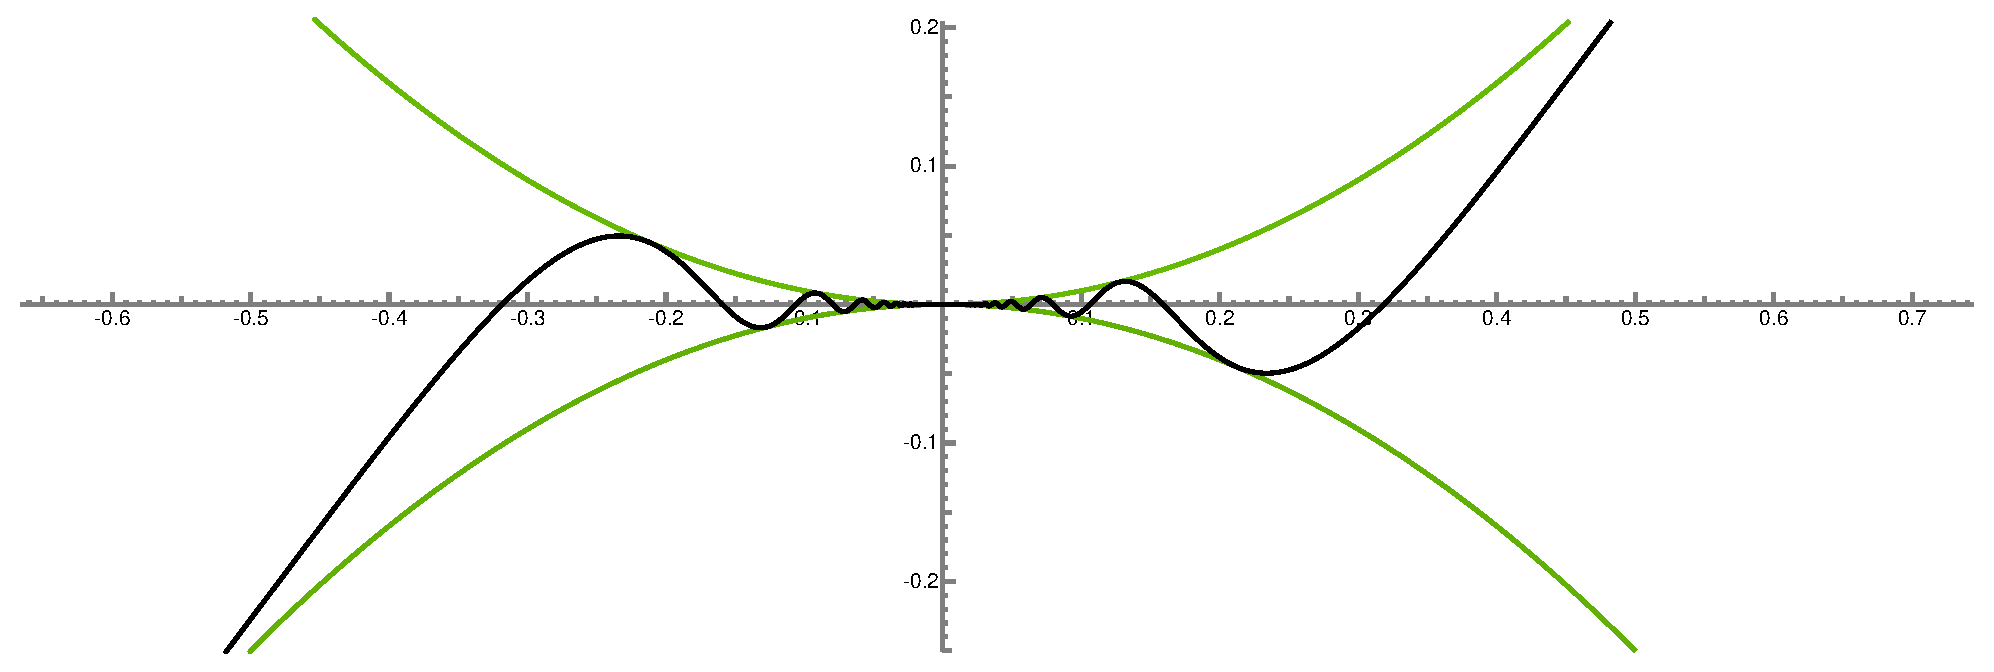
\includegraphics[height=4cm]{darboux.pdf}
  \centering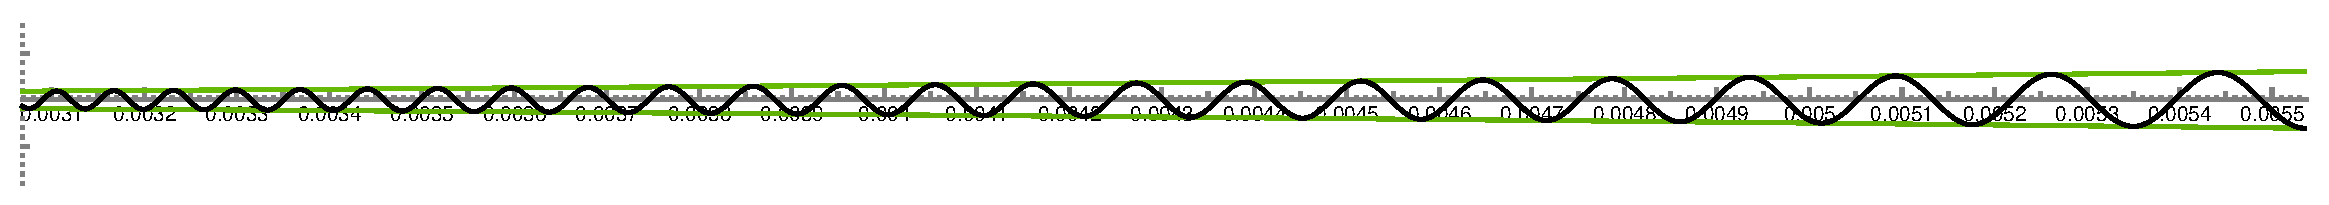
\includegraphics[width=\textwidth]{darboux2.pdf}
  \begin{comment}
  \begin{tikzpicture}[scale=5]
    \draw[->] (-0.5, 0) -- (0.5, 0) node[above] {$x$};
    \draw[->] (0, -0.3) -- (0, 0.3) node[right] {$y$};
    \draw[domain=-0.51:0.5, smooth, variable=\x, gray] plot ({\x}, {\x*\x});
    \draw[domain=-0.51:0.5, smooth, variable=\x, gray] plot ({\x}, {-\x*\x});
    \draw[domain=-0.51:0.5, variable=\x, samples=200, blue, thick] plot ({\x}, {\x*\x*sin(deg(1/\x))});
  \end{tikzpicture}
  \begin{tikzpicture}[scale=5000]
    \draw[->] (0.0045, 0) -- (0.0055, 0) node[above] {$x$};
    \draw[domain=0.0045:0.0055, smooth, variable=\x, gray] plot ({\x}, {\x*\x});
    \draw[domain=0.0045:0.0055, smooth, variable=\x, gray] plot ({\x}, {-\x*\x});
    \draw[domain=0.0045:0.0055, variable=\x, samples=200, blue, thick] plot ({\x}, {\x*\x*sin(deg(1/\x))});
  \end{tikzpicture}
  \end{comment}
  \caption{Il grafico di una funzione derivabile ma con 
    derivata non continua (vedi esempio~\ref{ex:derivata_non_continua}).
    L'ingrandimento nel disegno in basso rende evidente 
    il fatto che la derivata oscilla tra i valori 
    $-1$ e $1$ in ogni intorno di $0$.
    La proprietà di Darboux (teorema~\ref{th:darboux})
    rimane comunque soddisfatta: la derivata assume tutti i valori 
    compresi tra $1$ e $-1$ in ogni intorno di $x=0$ ma 
    non ha limite per $x\to 0$.\\\\
    \usebox{\qrdarboux}
}
\end{figure}

\begin{example}
[funzione derivabile con derivata non continua]
\label{ex:derivata_non_continua}%
\mymark{**}%
\index{funzione!derivabile con derivata non continua}%
\index{derivata!non continua}%
La funzione $f\colon \RR \to \RR$ definita da
\[
  f(x)
  = \begin{cases}
    x^2 \sin(1/x) & \text{se $x \neq 0$} \\
    0 & \text{se $x=0$.}
  \end{cases}
\]
è derivabile su tutto $\RR$, $f'(0)=0$ ma il limite
\[
\lim_{x\to 0} f'(x)
\]
non esiste (e dunque $f'\colon \RR\to\RR$ non è continua in $x=0$).
\end{example}
%
\begin{proof}
La funzione $x^2 \sin(1/x)$ è derivabile infinite volte su tutto il suo dominio $\RR\setminus\ENCLOSE{0}$ in quanto composizione di funzioni elementari derivabili infinite volte.
Dunque, per la località della derivata, anche la funzione $f$ è derivabile infinite volte su $\RR\setminus\ENCLOSE{0}$.
Per $x\neq 0$ possiamo quindi calcolare $f'(x)$ utilizzando le regole di derivazione
\[
  f'(x)
  = D \enclose{x^2\sin \frac 1 x}
  = 2x \sin \frac 1 x + x^2 \enclose{\cos \frac 1 x} \cdot\frac{-1}{x^2}
  = 2x \sin \frac 1 x - \cos \frac 1 x.
\]

Verifichiamo ora che $f$ è continua e derivabile anche in $0$.
Si ha infatti
\[
 \lim_{h\to 0}\frac{f(0+h)-f(0)}{h}
 = \lim_{h\to 0} h \sin \frac 1 h = 0
\]
e dunque $f'(0) = 0$.
Osserviamo però che $f'(x)$ non ammette limite per $x\to 0$
in quanto per $x \to 0$ si ha $2x \sin(1/x) \to 0$ ma il limite di $\cos (1/x)$ invece non esiste. Dunque $f'(x)$ è la somma di una funzione che ha limite zero e di una funzione il cui limite non esiste per $x\to 0$. Dunque $f'(x)$ non ammette limite per $x\to 0$.
\end{proof}

\begin{proposition}[criterio di derivabilità]%
\label{prop:4384774}\mymark{**}%
Sia $I\subset \RR$ un intervallo, $x_0\in I$,
$f\colon I \to \RR$ una funzione continua su tutto $I$ 
e derivabile in $I\setminus\ENCLOSE{x_0}$.
Se il limite della derivata
\[
  \lim_{x\to x_0} f'(x) = m
\]
esiste ed è finito la funzione $f$ è derivabile anche in $x_0$ e vale $f'(x_0) = m$.
\end{proposition}
%
\begin{proof}
\mymark{*}
Prendiamo un generico punto $x>x_0$ (il caso $x<x_0$ è del tutto analogo).
Per il teorema
di Lagrange sappiamo esistere un punto $y\in (x_0,x)$ tale che
\[
  \frac{f(x)-f(x_0)}{x-x_0} = f'(y).
\]
Per $x\to x_0$ si ha certamente anche $y\to x_0$ e dunque
esiste il limite del rapporto incrementale:
\[
  f'(x_0) = \lim_{x\to x_0} \frac{f(x)-f(x_0)}{x-x_0}
  = \lim_{y\to x_0} f'(y) = m.
\]
\end{proof}
%
La proposizione precedente dice che la derivata di una funzione in un
punto non può avere un valore diverso dal suo limite, se tale limite esiste.
Esistono però funzioni derivabili la cui derivata non è
continua, come abbiamo visto
nell'esempio~\ref{ex:derivata_non_continua}
in quanto il limite della derivata potrebbe non esistere.


\section{convessità}
\index{concavo}%
\index{convesso}%

\begin{definition}[funzione convessa]
\mymark{**}
Sia $I\subset \RR$ un intervallo.
Una funzione $f\colon I\to \RR$
si dice essere
\emph{convessa}
\mymargin{funzione convessa}%
\index{funzione!convessa}%
\index{convessa!funzione}%
se per ogni $x,y\in I$ e per ogni $t\in [0,1]$ si ha
\[
f((1-t)x + ty) \le (1-t) f(x) + t f(y).
\]

Analogamente diremo che $f$ è \emph{concava} 
\mymargin{funzione concava}%
\index{funzione!concava}%
\index{concava!funzione}%
se vale la disuguaglianza inversa:
\[
f((1-t)x + ty) \ge (1-t) f(x) + t f(y)
\]
(o, equivalentemente, se $-f$ è convessa).
\end{definition}

Osserviamo che la retta del piano passante per i punti $(x,f(x))$ e $(y,f(y))$ può essere parametrizzata in maniera uniforme per $t\in \RR$
da
\[
  (1-t) (x,f(x)) + t(y,f(y)) = ((1-t)x + ty, (1-t) f(x) + tf(y)).
\]
Chiaramente per $t=0$ si ottiene il punto $(x,f(x))$ per $t=1$ il punto $(y,f(y))$ e per $t\in[0,1]$ il segmento congiungente tali punti. La condizione di convessità della funzione $f$ corrisponde quindi a richiedere che ogni corda (segmento) che unisce due punti del grafico si trovi "al di sopra" del grafico della funzione.

\begin{definition}[insieme convesso]
\mymark{*}
Un insieme $E\subset \RR^n$ si dice essere \emph{convesso}%
\mymargin{convesso}%
\index{convesso} se dati
due punti qualunque $a,b\in E$ l'intero segmento $[a,b]=\ENCLOSE{(1-t)a+tb\colon t\in [0,1]}$ è contenuto in $E$.
\end{definition}

\begin{theorem}[epigrafico delle funzioni convesse]
Sia $I\subset \RR$ e $f\colon I\subset \RR\to \RR$ una funzione.
Allora sono equivalenti:
\begin{enumerate}
\item $I$ è un intervallo e $f$ è convessa;
\item l'\emph{epigrafico di $f$}%
\mymargin{epigrafico di $f$}%
\index{epigrafico}%
(o \emph{sopragrafico})
\index{epigrafico}%
ovvero l'insieme
\[
  E = \ENCLOSE{(x,y)\in \RR^2\colon x\in I, y\ge f(x)}
\]
è convesso.
\end{enumerate}

Per le funzioni concave sarà il \emph{sottografico} $\ENCLOSE{(x,y)\colon y\le f(x)}$ ad essere convesso.
\end{theorem}
%
\begin{proof}
Supponiamo che $I$ sia un intervallo e $f$ sia convessa. 
Per dimostrare che l'epigrafico $E$ è convesso consideriamo due punti $a,b\in E$ 
e un qualunque punto $p$ sul segmento $[a,b]$.
Se $a=(x_a, y_a)$, $b=(x_b,y_b)$, $p=(x_p, y_p)$
allora esiste un $t\in [0,1]$ tale che $x_p = (1-t)x_a + t x_b$ e $y_p=(1-t)y_a + t y_b$.
Visto che $a,b\in E$ sappiamo che $y_a \ge f(x_a)$ e $y_b\ge f(x_b)$. 
Dunque necessariamente si ha
\[
  y_p \ge (1-t)f(x_a) + t f(x_b).
\]
Ma essendo $f$ convessa si ha:
\[
  (1-t)f(x_a) + t f(x_b) \ge f((1-t)x_a + t x_b) = f(x_p).
\]
Dunque $y_p\ge f(x_p)$ che significa $p\in E$.

Viceversa supponiamo di sapere che $E$ è convesso. Siano $x,y\in I$ punti qualunque. Allora i punti $a=(x,f(x))$ e $b=(y,f(y))$ sono certamente punti di $E$ e quindi l'intero segmento $[a,b]$ deve essere contenuto in $E$. Dunque per ogni $t\in [0,1]$ il punto $p = ((1-t)x + t y,$ $(1-t)f(x)+ tf(y))$ deve stare in $E$. In primo luogo deve quindi essere $(1-t)x+ty\in I$ e se questo è vero per ogni $t\in[0,1]$ significa che $I$ è un intervallo. In secondo luogo se $p\in E$ significa che
\[
  (1-t)f(x) +t f(y) \ge f((1-t)x + t y)
\]
che corrisponde alla definizione di funzione convessa.
\end{proof}


\begin{lemma}[rapporto incrementale di una funzione convessa]
\mymark{*}%
\label{lemma:547091}%
Sia $I$ un intervallo di $\RR$ e sia $f\colon I\to \RR$.
Dati $x,y\in I$ con $x\neq y$ definiamo il \emph{rapporto incrementale}
di $f$ come:
\[
  R(x,y) = \frac{f(y) - f(x)}{y-x}.
\]
Allora sono condizioni equivalenti:
\begin{enumerate}
\item $f$ è convessa;
\item per ogni $x,y,z\in I$ se $x<y<z$ si ha $R(x,y)\le R(y,z)$;
\item per ogni $x,y,z\in I$ se $x<y<z$ si ha $R(x,y)\le R(x,z)$;
\item per ogni $x,y,z\in I$ se $x<y<z$ si ha $R(x,z)\le R(y,z)$;
\item la funzione $R(x,y)$ è crescente in ognuna delle due variabili.
\end{enumerate}
\end{lemma}
%
\begin{proof}
Attenzione:
il lemma risulta ovvio se si utilizza la giusta interpretazione geometrica
(il rapporto incrementale è la pendenza della corda corrispondente).
Quella che segue è la traduzione algebrica di quanto
è geometricamente ovvio ma risulta inevitabilmente pesante
e più difficilmente comprensibile.

Siano $x,y,z\in I$ con $x<y<z$.
Posto $t=(y-x)/(z-x)$ si ha $y=(1-t)x + tz$,
 $y-x = t(z-x)$, $z-y = (1-t)(z-x)$.
Si ha allora
 \begin{equation*}
 \begin{aligned}
 R(x,z) - R(x,y)
 &= \frac{f(z)-f(x)}{z-x} - \frac{f(y)-f(x)}{y-x} \\
  &= t\frac{f(z)-f(x)}{y-x} - \frac{f(y)-f(x)}{y-x} \\
  &= \frac{tf(z) + (1-t) f(x) - f(y)}{y-x}
 \end{aligned}
 \end{equation*}

La condizione di convessità di $f$ è
\[
  f(y) \le (1-t)f(x) + tf(z)
\]
ed è quindi equivalente alla condizione $R(x,y) \le R(x,z)$.
Dunque le condizioni 1 e 3 sono equivalenti.

Ma con una verifica diretta si osserva che
\[
  R(x,z) = t R(x,y) + (1-t) R(y,z)
\]
da cui si ottiene
\[
  R(y,z) - R(x,z) = t[R(y,z) - R(x,y)]
\]
oppure anche
\[
 R(x,z) - R(x,y) = (1-t) [R(y,z) - R(x,y)].
\]
Risulta quindi che le quantità
\[
  R(y,z) - R(x,y), \qquad
  R(x,z) - R(x,y), \qquad
  R(y,z) - R(x,z)
\]
hanno tutte lo stesso segno. E quindi le condizioni 2, 3 e 4 sono tra loro equivalenti (se vale una delle tre valgono tutte e tre).

Se valgono le tre condizioni 2, 3 e 4 è facile verificare che la funzione $R(x,y)$ è crescente in entrambe le variabili. Innanzitutto per simmetria, visto che $R(x,y) = R(y,x)$, è sufficiente verificare che $R(x,y)$ è crescente nella seconda variabile $y$ per ogni $x$ fissato. Quindi dato $z>y$ bisogna mostrare che $R(x,z) \ge R(x,y)$.
Abbiamo allora tre possibilità a seconda che sia $x<y$ oppure $y<x<z$ oppure $z<x$. Nel primo caso si ha $x<y<z$ e dunque la disuguaglianza $R(x,y) \le R(x,z)$ corrisponde alla condizione 3.
Nel secondo caso si ha $y<x<z$ e la condizione $R(x,y)\le R(x,z)$ si può scrivere come $R(y,x) \le R(x,z)$ che è, riordinando opportunamente le variabili, la condizione 2. Se, infine, $y < z < x$ la condizione $R(x,y) \le R(x,z)$ si può scrivere $R(y,x) \le R(z,x)$ che, riordinando le variabili, è la condizione 4.

Viceversa (e infine) se la funzione $R(x,y)$ è crescente in entrambe le variabili in particolare è crescente nella seconda variabile e quindi se $x<y<z$ si ha $R(x,y) \le R(x,z)$. Risulta quindi che la condizione 5 implica la 3 e quindi tutte le altre condizioni.
\end{proof}

\begin{theorem}
\mymark{***}
Sia $I\subset \RR$ un intervallo e $f\colon I \to \RR$ una funzione derivabile su tutto $I$.
Allora sono equivalenti:
\begin{enumerate}
\item $f$ è convessa;
\item per ogni $x_0 \in I$ e per ogni $x\in I$ si ha
\[
   f(x) \ge f'(x_0) (x-x_0) + f(x_0)
\]
(geometricamente: il grafico della funzione sta sopra la retta tangente);
\item $f'$ è crescente.
\end{enumerate}

Analogamente per le funzioni concave si avrà che il grafico ``sta sotto'' la retta tangente e che la derivata è decrescente.
\end{theorem}
%
\begin{proof}
\mymark{**}
Osserviamo che
\[
  f'(x_0) = \lim_{x\to x_0} R(x_0,x).
\]
Se $f$ è convessa allora, per il lemma, il rapporto incrementale $R(x_0,x)$ è crescente e quindi  $f'(x_0) = \inf_{x>x_0} R(x_0,x)$. In particolare $f'(x_0) \le R(x_0,x)$ per ogni $x> x_0$. In maniera analoga si trova $f'(x_0) \ge R(x_0,x)$ se $x<x_0$.
In ogni caso risulta quindi che per ogni $x$ si ha
\[
(R(x_0,x)- f'(x_0))(x-x_0)\ge 0
\]
ovvero
\[
  f(x) - f(x_0) - f'(x_0)(x-x_0) \ge 0.
\]
Dunque la condizione 1 implica la 2.

Se vale la condizione 2, dati $x,y \in I$ si ha
\[
  f(x) - f(y) \ge f'(y)(x-y)
\]
se scambiamo $x$ e $y$ e cambiamo di segno ambo i membri si ottiene invece
\[
  f(x) - f(y) \le f'(x)(x-y)
\]
mettendo insieme le due disuguaglianze,
se ora supponiamo che sia $x>y$ otteniamo proprio
$f'(x) \ge f'(y)$ cioè $f'$ è crescente (condizione 3).

Supponiamo ora di sapere che $f'$ è crescente 
e dimostriamo che se $x<y<z$ allora $R(x,y) \le R(y,z)$.
Per il teorema di Lagrange esistono $s\in (x,y)$ 
e $t\in (y,z)$ tali che $f'(s) = R(x,y)$ e $f'(t) = R(y,z)$.
Ma $s<t$ dunque $f'(s) \le f'(t)$ ovvero $R(x,y) \le R(y,z)$
come volevamo dimostrare.
\end{proof}

\begin{corollary}[criterio di convessità tramite derivata seconda]
\mymark{***}
Sia $I\subset \RR$ un intervallo e sia $f\colon I \to \RR$ una funzione derivabile due volte (cioè $f$ è derivabile e anche $f'$ è derivabile).
Allora $f$ è convessa se e solo se $f''(x)\ge 0$ per ogni $x\in I$.
Analogamente $f$ è concava se e solo se $f''\le 0$.
\end{corollary}
\begin{proof}
\mymark{***}
Per il criterio precedente $f$ è convessa se e solo se $f'$ è crescente. Per il criterio di monotonia $f'$ è crescente se e solo se $f'' \ge 0$. Considerazioni analoghe valgono per la concavità.
\end{proof}

\begin{theorem}
Siano $a\in \RR$, $b\in \bar \RR$, $a<b$.
Sia $f\colon [a,b)\to \RR$ una funzione convessa 
in $(a,b)$ e continua in $a$. 
Allora $f$ è convessa su tutto $[a,b)$. 
Risultato analogo vale per funzioni definite su 
intervalli aperti a sinistra $(a,b]$
o su intervalli aperti da ambo i lati $(a,b)$.
\end{theorem}
%
\begin{proof}
Basta dimostrare che se $x<y<z$ allora $R(x,y)\le R(y,z)$.
La disuguaglianza è valida per $x>a$ essendo $f$ convessa 
in $(a,b)$ e dunque, passando al limite per $x\to a$, 
grazie alla continuità di $f$ in $a$,
la disuguaglianza risulta dimostrata anche quando $x=a$.
\end{proof}

\begin{example}
La funzione $f(x) = \sqrt{x}$ è definita su $[0,+\infty)$ ma è derivabile solamente in $(0,+\infty)$. La sua derivata è $f'(x) = x^{-\frac 1 2 }/2$ e la derivata seconda è $f''(x) = -x^{-\frac 3 2}/4 < 0$. Dunque la funzione è concava sull'intervallo aperto $(0,+\infty)$. Ma essendo continua possiamo concludere che $f$ è concava su tutto il dominio $[0,+\infty)$.
\end{example}

\begin{comment}
\begin{theorem}[continuità delle funzioni convesse]
Siano $a,b \in \bar \RR$ con $a< b$.
Sia $f\colon (a,b) \to \RR$ una funzione convessa. Allora $f$ è continua.
\end{theorem}
%
\begin{proof}
Sia $x_0 \in (a,b)$ e siano $y,z \in (a,b)$ con $y < x_0 < z$.
Per il lemma sui rapporti incrementali sappiamo che per ogni $x\in (y,z)$ si ha
\[
   R(x_0, y) \le R(x_0,x) \le R(x_0,z).
\]
In particolare esiste una costante $C$ tale che
\[
  \abs{R(x_0,x)} \le C,\qquad \forall x \in (y,z).
\]
Moltiplicando per $\abs{x-x_0}$ si ottiene allora
\[
   \abs{f(x) - f(x_0)} \le C \abs{x-x_0}
\]
e per $x\to x_0$ il lato destro tende a zero e quindi per confronto anche il lato sinistro deve tendere a zero. Dunque $f(x)\to f(x_0)$
e $f$ è continua in $x_0$.
\end{proof}
\end{comment}

\begin{theorem}[derivabilità delle funzioni convesse]
  Sia $I\subset \RR$ un intervallo e sia $f\colon I \to \RR$ una funzione convessa.
  Se $x_0\in (\inf I, \sup I)$ esistono e sono finite la derivata destra 
  e sinistra di $f$ in $x_0$:
  \begin{align*}
    f'_+(x_0) &= \lim_{x\to x_0^+} \frac{f(x)-f(x_0)}{x-x_0}\\
    f'_-(x_0)  &= \lim_{x\to x_0^-} \frac{f(x)-f(x_0)}{x-x_0}  
  \end{align*}
  e risulta
  \[
    f'_-(x_0) \le f'_+(x_0).
  \]
  Inoltre se $\inf I < x_1 < x_2 < \sup I$ si ha 
  \[
    f'_+(x_1) \le f'_-(x_2).
  \]
  Se ne deduce che $f$ è continua in tutti i punti interni di $I$ 
  e che l'insieme dei punti in cui $f$ non è derivabile 
  è al più numerabile.
  \end{theorem}
  %
  \begin{proof}
    Nel lemma~\ref{lemma:547091} abbiamo osservato che il rapporto incrementale
    \[
      R(x_0,x) = \frac{f(x)-f(x_0)}{x-x_0}
    \] 
    di una funzione convessa è crescente rispetto alla variabile $x$. 
    Dunque per il teorema~\ref{th:limite_funzione_monotona} si 
    ha 
    \[
      f'_-(x_0) = \sup_{x<x_0} R(x_0,x)>-\infty, \qquad 
      f'_+(x_0) = \inf_{x>x_0} R(x_0,x)<+\infty
    \]
    e visto che se $x<x_0$ e $y>x_0$ si ha $R(x_0,x)\le R(x_0,y)$ 
    deduciamo che $f'_-(x_0)\le f'_+(x_0)$ ed entrambi i limiti 
    sono dunque finiti. Se $x_1 < x_2$ allora preso un qualunque 
    punto $x$ con $x_1<x<x_2$ si ha (sempre per il lemma~\ref{lemma:547091})
    \[
      R(x_1,x) \le R(x,x_2)
    \]
    e dunque passando al limite si trova $f'_+(x_1) \le f'_-(x_2)$.
    Le derivate destra e sinistra esistono dunque in tutti i punti interni 
    all'intervallo $I$. 
    In particolare $f$ è continua in tali punti in quanto è continua sia da destra 
    che da sinistra.
    I punti di non derivabilità di $f$ sono i punti in cui 
    le derivate destra e sinistra differiscono. 
    Ma ad ogni punto $x$ di non differenziabilità 
    posso associare l'intervallo aperto non vuoto $I_x = (f'_-(x),f'_+(x))$ e per 
    le proprietà appena viste è chiaro che questi intervalli sono a due a due disgiunti
    in quanto se $x_1<x_2$ l'estremo destro di $I_{x_1}$ è minore o uguale all'estremo 
    sinistro di $I_{x_2}$.
    Siccome ognuno di questi intervalli contiene almeno un numero razionale concludiamo che 
    il numero di punti di discontinuità non può essere maggiore della cardinalità 
    dei numeri razionali.
  \end{proof}
  
  \begin{theorem}[retta di supporto]
    \label{th:supporto_convessa}%
    Sia $I\subset \RR$ un intervallo, $f\colon I\to\RR$ una funzione convessa 
    e $x_0$ un punto interno ad $I$. Allora esiste una funzione lineare affine 
    \[
      L(x) = mx+q
    \]
    tale che $f(x_0) = L(x_0)$ e per ogni $x\in I$ si abbia $f(x)\ge L(x)$.
  \end{theorem}
  %
  \begin{proof}
    Basta scegliere qualunque $m\in [f'_-(x_0),f'_+(x_0)]$ e considerare la funzione 
    lineare affine $L(x) = m(x-x_0) + f(x_0)$. Se $x>x_0$ allora si ha $R(x_0,x)\ge m$ 
    e dunque $f(x) - f(x_0) \ge m (x-x_0) = L(x)$. Viceversa se $x<x_0$ 
    si ha $R(x_0,x)\le m$ da cui, di nuovo, $f(x)-f(x_0) \ge m(x-x_0) = L(x)$.
  \end{proof}
  %
  Il seguente teorema può essere enunciato anche per gli integrali 
  come vedremo nel teorema~\ref{th:jensen}. 
  La dimostrazione è sostanzialmente identica ed è valida anche 
  per funzioni convesse di più variabili.
  %
  \begin{theorem}[combinazioni baricentriche/disuguaglianza di Jensen]
    \mymark{*}%
    \label{th:combinazioni_baricentriche}%
    \index{combinazioni baricentriche}%
    \index{disuguaglianza!di Jensen}%
    \index{Jensen!disuguaglianza di}%
    Se $f$ è una funzione convessa definita su un intervallo $I$, dati $x_1, \dots, x_n \in I$ e $\lambda_1, \dots, \lambda_n\in \RR$ tali che $\sum_{k=1}^n \lambda_k = 1$ e $\lambda_k \ge 0$ per ogni $k=1, \dots, n$ allora
    \[
      f\enclose{\sum_{k=1}^n \lambda_k x_k}
      \le \sum_{k=1}^n \lambda_k f(x_k).
    \]
    Per le funzioni concave vale la disuguaglianza inversa.
    \end{theorem}
    %
    \begin{comment}
    \begin{proof}
    Procediamo per induzione su $n$. Nel caso $n=1$ si ha $\lambda_1=1$ e i due lati della disuguaglianza sono effettivamente uguali. Supponendo il teorema dimostrato per un certo $n$, procediamo a dimostrarlo per $n+1$.
    Osserviamo che
    \begin{align*}
      \sum_{k=1}^{n+1} \lambda_k x_k
      &= \sum_{k=1}^n \lambda_k x_k  + \lambda_{n+1} x_{n+1} \\
      &= (1-\lambda_{n+1})\sum_{k=1}^n\frac{\lambda_k}{1-\lambda_{n+1}} x_k + \lambda_{n+1} x_{n+1}.
    \end{align*}
    Visto che
    \[
      \sum_{k=1}^{n+1} \lambda_k = 1
    \]
    si ha
    \[
      \sum_{k=1}^n \frac{\lambda_k}{1-\lambda_{n+1}}
      = \frac{1-\lambda_{n+1}}{1-\lambda_{n+1}} = 1.
    \]
    Dunque, per ipotesi induttiva si ha allora
    \[
      f\enclose{\sum_{k=1}^n\frac{\lambda_k}{1-\lambda_{n+1}} x_k}
      \le \sum_{k=1}^n \frac{\lambda_k}{1-\lambda_{n+1}}f(x_k).
    \]
    Usando di nuovo la convessità di $f$ con $t=\lambda_{n+1}$ si ha
    \begin{align*}
    f\enclose{\sum_{k=1}^{n+1} \lambda_k x_k}
    &=f\enclose{(1-\lambda_{n+1})\sum_{k=1}^n \frac{\lambda_k}{1-\lambda_{n+1}}x_k + \lambda_{n+1}x_{n+1}}\\
    &\le (1-\lambda_{n+1})f\enclose{\sum_{k=1}^n \frac{\lambda_k}{1-\lambda_{n+1}}x_k} + \lambda_{n+1}f(x_{n+1}) \\
    &\le (1-\lambda_{n+1})\sum_{k=1}^n \frac{\lambda_k}{1-\lambda_{n+1}} f(x_k) + \lambda_{n+1} f(x_{n+1})\\
    &= \sum_{k=1}^{n+1}\lambda_k f(x_k).
    \end{align*}
    come volevamo dimostrare.
    \end{proof}
  \end{comment}
  %    
  \begin{proof}
  Poniamo 
  \[
    \bar x =  \sum_{k=1}^n \lambda_k x_k.
  \]
  Per il teorema~\ref{th:supporto_convessa} precedente 
  sappiamo che esiste una retta $L(x) = mx + q$ 
  tale che $L(\bar x) = f(\bar x)$ 
  e $L(x)\le f(x)$ per ogni $x \in I$.
  Allora si ha 
  \[
  L \enclose{\sum_{k=1}^n \lambda_k x_k}
  = \sum_{k=1}^n m \lambda_k x_k + q \sum_{k=1}^n \lambda_k 
  = \sum_{k=1}^n \lambda_k L(x_k).  
  \]
  Dunque 
  \[
  f(\bar x) = L(\bar x) = \sum_{k=1}^n \lambda_k L(x_k) \le 
  \sum_{k=1}^n \lambda_k f(x_k).
  \]
  \end{proof}

\begin{example}[disuguaglianza tra media aritmetica e media geometrica]
\label{ex:AMGM}%
  \mymark{*}%
\index{disuguaglianza!media aritmetica media geometrica}%
Osserviamo che la funzione $f(x) = \ln x$ è concava, infatti si ha
$f''(x) = -1/x^2 < 0$. Dunque, per il teorema precedente, se $\lambda_1 + \dots + \lambda_n =1$, $\lambda_k \ge 0$ si ha
\[
    \ln\enclose{\sum_{k=1}^n \lambda_k x_k}
    \ge \sum_{k=1}^n \lambda_k \ln x_k.
\]
Facendo l'esponenziale di ambo i membri si ottiene
\[
  \sum_{k=1}^n \lambda_k x_k \ge \prod_{k=1}^n x_k^{\lambda_k}.
\]
Nel caso particolare $\lambda_k = 1/n$ si ottiene
la disuguaglianza tra \emph{media aritmetica} (AM per gli anglofoni)
e \emph{media geometrica}
\mymargin{media aritmetica geometrica}%
\index{media aritmetica geometrica}%
\index{media!aritmetica}%
\index{media!geometrica}%
\index{AM}%
\index{GM}%
(GM):
\[
  \frac{x_1 + \dots + x_n}{n} \ge \sqrt[n]{x_1\cdots x_n}.
\]
\end{example}

\begin{exercise}[subadditività delle funzioni concave]
\index{subadditività!delle funzioni concave}%
\index{funzione!concava!subadditiva}%
\index{concavo!subadditiva}%
Sia $f\colon [0,+\infty) \to \RR$ una funzione concava con $f(0)\ge 0$. Allora $f$ è subadditiva cioè:
\[
  f(x+y) \le f(x) + f(y),\qquad \forall x,y\ge 0.
\]
\end{exercise}
%
\begin{proof}
Se $x=y=0$ la disuguaglianza è ovvia.
Altrimenti $x+y>0$ e si ha
\begin{align*}
f(x) &= f\enclose{\frac{y}{x+y}\cdot 0 + \frac{x}{x+y}\cdot (x+y)}\\ &\ge \frac{y}{x+y}f(0) + \frac{x}{x+y}f(x+y)
\ge \frac{x}{x+y}f(x+y).
\end{align*}
Scambiando $x$ con $y$ e sommando si ottiene:
\[
  f(x) + f(y) \ge \frac{x}{x+y}f(x+y) + \frac{y}{x+y}f(x+y) = f(x+y).
\]
\end{proof}

Si osservi che sviluppando la disuguaglianza $(x-y)^2\ge 0$ si ottiene:
\[
  x y \le \frac{x^2 + y^2}{2}.
\]
Questa disuguaglianza può essere generalizzata ad esponenti diversi 
come si vede nel seguente.

\begin{theorem}[disuguaglianza di Young]%
\label{th:young}%
\index{Young!disuguaglianza di}%
\index{disuguaglianza!di Young}%
Se $p>1$, $q>1$, $\frac{1}{p}+\frac{1}{q}=1$, $x,y\ge 0$:
\begin{equation}\label{eq:young}
  x y \le \frac{x^p}{p} + \frac{y^q}{q}.
\end{equation}
\end{theorem}
%
\begin{proof}
Si utilizza la disuguaglianza di convessità per la funzione $\exp(x)=e^x$. 
Visto che la derivata seconda dell'esponenziale è positiva, la funzione $\exp$ 
è convessa e dunque, se $x>0$ e $y>0$ si ha:
\begin{align*}
 x\cdot y 
  &= \exp(\ln x + \ln y)
  = \exp\enclose{\frac 1 p \ln (x^p) + \frac 1 q \ln (y^q)}  \\
  &\le \frac 1 p \cdot \exp \ln (x^p) + \frac 1 q \exp \ln (y^q)
  = \frac{x^p}{p} + \frac{y^q}{q}.
\end{align*}
Se $x=0$ o $y=0$ la disuguaglianza è ovvia in quanto il lato sinistro 
di~\eqref{eq:young} è nullo.
\end{proof}

\begin{theorem}[disuguaglianza di Hölder]
Se $a_k\ge 0$ e $b_k\ge 0$ per $k\in \NN$
e siano $p>1$ e $q>1$ tali che $\frac 1 p + \frac 1 q = 1$.
Allora 
\[
 \sum_k a_k b_k  \le \enclose{\sum_k a_k^p}^{1 \over p} \cdot \enclose{\sum_k b_k^q}^{1\over q}.
\]
\end{theorem}
\begin{proof}
Poniamo 
\[
A = \enclose{\sum_k a_k^p}^{1 \over p}, \qquad 
B = \enclose{\sum_k b_k^q}^{1\over q}.
\]
Se $A>0$ e $B>0$ possiamo dividere il lato sinistro della disuguaglianza 
per il lato destro e applicare la disuguaglianza~\eqref{eq:young} di Young:
\begin{align*}
  \frac{\sum_k a_k b_k}{A\cdot B} 
  & = \sum_k \frac{a_k}{A}\cdot \frac{b_k}{B} 
  \le \sum_k \frac 1 p \frac{a_k^p}{A^p} + \frac 1 q \frac{b_k^q}{B^q} \\
  &= \frac 1 p \frac{\sum_k a_k^p}{A^p} + \frac 1 q \frac{\sum_k b_k^q}{B^q}
  = \frac 1 p + \frac 1 q = 1.
\end{align*}
E il teorema e dimostrato. 

Se fosse $A=0$ tutti i termini $a_k$ sarebbero nulli e la disuguaglianza 
si riduce banalmente a $0\le 0$. Lo stesso se fosse $B=0$.  
\end{proof}

Nel caso $p=q=2$ si ottiene la 
\emph{disuguaglianza di Cauchy-Schwarz}%
\mymargin{disuguaglianza di Cauchy-Schwarz}%
\index{disuguaglianza!di Cauchy-Schwarz}
\index{disuguaglianza!di Cauchy-Schwarz}%
\index{Cauchy-Schwarz!disuguaglianza di}%
\index{Schwarz!disuguaglianza di Cauchy-}%
\[
   \sum_k \abs{a_k b_k} \le \sqrt{\sum_k a_k^2} \cdot \sqrt{\sum_k b_k^2}
\]
che potrebbe però essere più facilmente dimostrata 
per un generico prodotto scalare, come faremo 
nel teorema~\ref{th:spazio_euclideo}.


\section{teoremi di Cauchy e de l'Hospital}

\begin{theorem}[Cauchy]
\label{th:cauchy}%
\mymark{**}%
\index{teorema!di Cauchy}%
\mymargin{Cauchy}%
\index{Cauchy}%
Siano $a,b\in \RR$, $a < b$.
\mynote{Se $b<a$ il teorema è ugualmente valido intendendo $[a,b]=[b,a]$.}%
Siano $f\colon[a,b]\to \RR$ e $g\colon[a,b]\to \RR$ funzioni continue su tutto $[a,b]$ e derivabili su $(a,b)$.
Supponiamo inoltre che $g'(x)\neq 0$ per ogni $x\in (a,b)$.
Allora $g(b) \neq g(a)$ ed esiste $x_0\in(a,b)$ tale che
\[
  \frac{f'(x_0)}{g'(x_0)} = \frac{f(b)-f(a)}{g(b)-g(a)}.
\]
\end{theorem}
%
\begin{proof}
\mymark{**}
Si consideri la funzione ausiliaria
\[
 h(x) = (g(b)-g(a))f(x) - (f(b)-f(a))g(x).
\]
Per verifica diretta si osserva che
\[
  h(b) = g(b)f(a) - f(b)g(a) = h(a).
\]
Dunque $h$ verifica le ipotesi del teorema di Rolle ed esiste
dunque un punto $x_0\in(a,b)$ per cui $h'(x_0) = 0$.
Essendo però
\[
  h'(x) = (g(b) - g(a)) f'(x) - (f(b)-f(a)) g'(x)
\]
si ottiene
\[
 (g(b)-g(a))f'(x_0) = (f(b) - f(a))g'(x_0).
\]
Per ipotesi sappiamo che $g'(x_0)\neq 0$.
Ma necessariamente anche $g(b) - g(a)\neq 0$ perché altrimenti potremmo applicare il teorema di Rolle alla funzione $g$ e ottenere che $g'$ si annulla in un punto di $(a,b)$, cosa che abbiamo escluso per ipotesi.
Dunque possiamo dividere ambo i membri per $(g(b)-g(a))$ e per $g'(x_0)$ per ottenere l'uguaglianza enunciata nel teorema.
\end{proof}

\begin{theorem}[de l'Hospital $0/0$]
\mymark{***}
Sia $I\subset \RR$ un intervallo, $x_0\in [-\infty,+\infty]$ un punto di accumulazione
di $I$
e siano $f,g \colon I\setminus\ENCLOSE{x_0} \to \RR$ funzioni derivabili.
Supponiamo che sia $g'(x)\neq 0$ per ogni $x\in I\setminus\ENCLOSE{x_0}$.
Se
\[
  \lim_{x\to x_0} f(x) = 0 \qquad \text{e}\qquad \lim_{x\to x_0} g(x) = 0
\]
e se esiste (finito o infinito) il limite
\[
  \ell = \lim_{x\to x_0}\frac{f'(x)}{g'(x)}
\]
allora si ha
\[
  \lim_{x\to x_0} \frac{f(x)}{g(x)} = \ell.
\]
\end{theorem}
%
\begin{proof}
\mymark{**}
Bisognerà distinguere diversi casi a seconda che $x_0$ sia finito o infinito
e che sia un punto interno o un estremo dell'intervallo $I$.
Fatta la dimostrazione nel primo caso tutti gli altri si riconducono ad esso.

\emph{Caso 1:} supponiamo che sia $I=[x_0, b]$. In questo caso possiamo
estendere le funzioni $f$ e $g$ anche nel punto $x_0$ ponendo:
\[
\tilde f(x) =
\begin{cases}
  f(x) & \text{se $x\in (x_0,b]$}\\
  0 & \text{se $x=x_0$,}
\end{cases}
\qquad
\tilde g(x) =
\begin{cases}
  g(x) & \text{se $x\in (x_0,b]$}\\
  0 & \text{se $x=x_0$.}
\end{cases}
\]
Visto che per ipotesi $f(x) \to 0$ e $g(x)\to 0$ per $x\to x_0$ risulta
che $\tilde f$ e $\tilde g$ siano funzioni continue su tutto l'intervallo $[x_0,b]$
inoltre, sempre per ipotesi, sono derivabili nell'intervallo $(x_0,b]$
visto che l'estensione per $x=x_0$ non modifica le derivate negli altri punti.
In particolare le funzioni estese soddisfano le ipotesi del teorema di Cauchy in
ogni intervallo $[x_0,x]$ con $x\in (x_0,b]$, dunque possiamo affermare
che per ogni $x$ esiste $c(x)\in (x_0,x)$ tale che
\[
  \frac{f(x)}{g(x)}
  = \frac{\tilde f(x) - \tilde f(x_0)}
  {\tilde g(x)- \tilde g(x_0)}
  = \frac{\tilde f'(c(x))}{\tilde g'(c(x))}
  = \frac{f'(c(x))}{g'(c(x))}.
\]
Ma essendo $x_0< c(x) < x$ per $x\to x_0$ si ha $c(x)\to x_0$ e quindi,
tramite un cambio di variabile
(Teorema~\ref{th:limite_composta})
possiamo affermare che
\[
    \lim_{x\to x_0} \frac{f(x)}{g(x)}
  = \lim_{x\to x_0}\frac{f'(c(x))}{g'(c(x))}
  = \lim_{x\to x_0}\frac{f'(x)}{g'(x)} = \ell.
\]

\emph{Caso 2:} supponiamo sia $I$ qualunque e $x_0$ finito.
Visto che le funzioni sono definite su $I\setminus\ENCLOSE{x_0}$ possiamo sempre
supporre $x_0\in I$. Inoltre
visto che i limiti dipendono solo dai valori in un intorno del punto $x_0$
possiamo sempre supporre che $I$ sia un intervallo chiuso e limitato.
Nel passo precedente abbiamo fatto il caso in cui $x_0$ era l'estremo
inferiore di $I$, ma allo stesso modo si può fare il caso in cui
$x_0$ è l'estremo superiore. Se invece $x_0$ fosse un punto interno di $I$
possiamo considerare separatamente il limite destro e sinistro e ricondurci
ai casi in cui $x_0$ era un estremo.

\emph{Caso 3:} supponiamo sia $x_0=+\infty$. In tal caso
l'intervallo $I$ contiene un intevallo $[a,+\infty)$ con $a\in\RR$.
Anche in questo caso vogliamo ricondurci al primo caso tramite il cambio
di variabile $t=1/x$. Posto $F(t) = f(1/t)$ e $G(t)= g(1/t)$ si osserva che $F$ e $G$
sono definite sull'intervallo $(0,1/a]$,
tendono a zero per $t\to 0^+$
sono derivabili,
\[
  F'(t) = -\frac{f'(1/t)}{t^2}, \qquad
  G'(t) = -\frac{g'(1/t))}{t^2}
\]
e risulta quindi
\[
  \lim_{t\to 0^+} \frac{F'(t)}{G'(t)}
  = \lim_{t\to 0^+} \frac{f'(1/t)}{g'(1/t)}
  = \lim_{x\to +\infty} \frac{f'(x)}{g'(x)} = \ell.
\]
Quindi applicando il teorema nel caso già dimostrato possiamo affermare che
\[
  \lim_{x\to +\infty} \frac{f(x)}{g(x)} = \lim_{t\to 0^+} \frac{F(t)}{G(t)} = \ell.
\]

\emph{Caso 4:} il caso $x_0 = -\infty$ si svolge in maniera analoga al caso precedente.
\end{proof}

\begin{theorem}[de l'Hospital $\cdot/\infty$]
\mymark{*}
\index{teorema!di de l'Hospital}
\mymargin{de l'Hospital}%
\index{de l'Hospital}
Siano $a,b\in [-\infty,+\infty]$ con $a<b$.
Siano $f,g \colon (a,b)\to \RR$ funzioni derivabili.
Se
\[
 \lim_{x\to a^+} \abs{g(x)} = +\infty,
\]
se $g'(x) \neq 0$ per ogni $x\in (a,b)$
e se esiste il limite (finito o infinito)
\[
  \ell = \lim_{x\to a^+}\frac{f'(x)}{g'(x)}
\]
allora
si ha
\[
 \lim_{x\to a^+}\frac{f(x)}{g(x)} = \ell.
\]

Risultato analogo si ha facendo i limiti per $x\to b^-$ invece che per $x\to a^+$ e di conseguenza anche nel caso in cui la funzione sia definita su un intervallo ``bucato''
$f\colon (a,b)\setminus\ENCLOSE{x_0} \to \RR$ e si considerino i limiti ``pieni'' per $x\to x_0$.
\end{theorem}
%
\begin{proof}
Supponiamo per assurdo che non si abbia
\[
  \lim_{x\to a^+} \frac{f(x)}{g(x)} = \ell.
\]
Allora, per il teorema di collegamento tra limiti di funzione e limiti di successione, deve esistere una successione $a_k\in (a,b)$, $a_k\to a$ tale che non si abbia
\[
  \lim_{k\to +\infty} \frac{f(a_k)}{g(a_k)} = \ell.
\]
Se la successione $f(a_k) / g(a_k)$ è limitata allora applicando il teorema di Bolzano Weierstrass sappiamo esistere una sottosuccessione
convergente ad un valore $m\neq \ell$ (se tutte le sottosuccessioni convergessero ad $\ell$ l'intera successione convergerebbe ad $\ell$).
Se invece $f(a_k) / g(a_k)$ non è limitata possiamo estrarre una sottosuccessione che diverge a $+\infty$ oppure a $-\infty$. In ogni caso esiste una successione, che chiameremo ancora $a_k$, ed esiste $m\in \bar \RR$ tale che
\[
  \lim_{k \to +\infty} \frac{f(a_k)}{g(a_k)} = m \neq \ell.
\]
Consideriamo ora un intorno $U$ di $m$ e un intorno $V$ di $\ell$ tali che $U\cap V = \emptyset$.
Siccome $f'(x) / g'(x) \to \ell$ per $x\to a$ esiste un $c\in (a,b)$ tale che per ogni $x\in (a,c)$ si ha
\[
  \frac{f'(x)}{g'(x)} \in V.
\]
Consideriamo allora il seguente rapporto incrementale
\begin{align*}
\frac{f(a_k) - f(x)}{g(a_k) - g(x)}
=\frac{\frac{f(a_k)}{g(a_k)}-\frac{f(x)}{g(a_k)}}{1-\frac{g(x)}{g(a_k)}}
\end{align*}
e osserviamo che il lato destro tende a $m$ per $k\to +\infty$ in quanto $f(a_k)/g(a_k) \to m$ e visto che $\abs{g(a_k)}\to +\infty$ si ha $f(x)/g(a_k)\to 0$ e $g(x)/g(a_k) \to 0$.
Dunque esisterà un $k$ per cui il lato destro sta nell'intorno $U$ di $m$. Al lato sinistro possiamo invece applicare il teorema di Cauchy e trovare quindi un punto $y\in(a_k,c)$ per cui tale lato risulti
uguale a $f'(y)/g'(y)$. Ma visto che $y\in (a,c)$ si dovrà avere $f'(y)/g'(y) \in V$. Questo è assurdo in quanto $U\cap V = \emptyset$.
\end{proof}


\section{classi di regolarità}

Sia $A\subset \RR$ e sia $f\colon A\to \RR$ una funzione definita su $A$.
Diremo che $f$ è di classe $C^0$ se $f$ è continua. 
Possiamo definire $C^0(A)$ come l'insieme delle funzioni continue definite 
su $A$ (a valori in $\RR$).
Se $f$ è derivabile (su tutto $A$) e la derivata di $f$ è anch'essa continua 
(su tutto $A$) diremo che 
$f$ è di classe $C^1$ e scriveremo $f\in C^1(A)$.
Andando avanti: se $f$ è derivabile e anche $f'$ è derivabile e se la derivata 
seconda $f''$ è continua, diremo che $f$ è di classe $C^2$. 
E così via.

E' importante osservare che $C^1(A)$ non coincide con l'insieme delle funzioni 
derivabili su $A$. 
Infatti abbiamo già visto nell'esempio~\ref{ex:derivata_non_continua} 
che esistono funzioni derivabili la cui derivata non è continua 
e quindi tali funzioni, pur essendo derivabili, non sono di classe $C^1$.


Per definire formalmente l'insieme delle funzioni di classe $C^k$ 
per ogni $k\in \NN$ dobbiamo dare una definizione per induzione.
Definiamo inoltre la classe $C^{\infty}(A)$ che è l'insieme delle funzioni 
che sono derivabili $k$ volte per ogni $k\in \NN$.
%
\begin{definition}[funzioni di classe $C^k$]
\mymark{**}
Dato $A\subset \RR$ denotiamo con $\RR^A$ l'insieme di tutte le funzioni $f\colon A \to \RR$.
Per ogni $k\in \NN$ definiamo
$C^k(A) \subset \RR^A$ nel modo seguente:
\mymargin{$C^k$}%
\index{$C^k$}
\begin{enumerate}
\item se $k=0$ poniamo
\[
  C^0(A) = \ENCLOSE{f\in \RR^A \colon \text{$f$ continua}}.
\]
\item
  se $k>0$ definiamo induttivamente
  \[
  C^{k}(A) = \ENCLOSE{f\in \RR^A \colon \text{$f$ derivabile e $f'\in C^{k-1}(A)$}}.
  \]
\end{enumerate}
Chiaramente se $j\ge k$ si ha $C^j(A) \subset C^k(A)$ dunque $C^k(A)$ è una famiglia decrescente (rispetto all'inclusione insiemistica) ed ha senso definire:
\mymargin{$C^\infty$}%
\index{$C^\infty$}
\[
  C^\infty(A) = \ENCLOSE{f\in \RR^A\colon \forall k \in \NN\colon f\in C^k(A)} = \bigcap_{k\in \NN} C^k(A).
\]

Le funzioni $f\in C^k(A)$ sono derivabili $k$ volte.
Utilizziamo la notazione $f^{(j)}$%
\mymargin{$f^{(j)}$}%
\index{$f^{(j)}$} per denotare la $j$-esima derivata
di una funzione $f$.
Dunque avremo
\[
  f^{(0)} = f, \qquad
  f^{(1)} = f', \qquad
  f^{(2)} = f'', \dots
\]
\end{definition}

Abbiamo già osservato che $\RR^A$ è uno spazio vettoriale reale.
Gli spazi $C^k(A)$ per $k=0, \dots, \infty$ sono una famiglia decrescente di sottospazi vettoriali di $\RR^A$.
Infatti sappiamo che la combinazione lineare di funzioni continue è continua e che la combinazione lineare di funzioni derivabili è derivabile.

\begin{theorem}
Le funzioni $x$, $e^x$, $\ln x$, $\sin x$, $\cos x$, $\tg x$, $\arctg x$ 
sono di classe $C^\infty$. 
Somma, differenza, prodotto, rapporto, e composizione di funzioni di classe $C^n$ 
sono anch'esse di classe $C^n$ per $n=0,1,2,\dots,\infty$.
\end{theorem}
\begin{proof}
Verifichiamo per induzione che se $f,g \in C^n$ allora $f+g \in C^n$.
Per $n=0$ sappiamo che la somma di funzioni continue è continua: $f,g\in C^0$ implica $f+g\in C^0$.
Per $n>1$ se $f,g\in C^n$ allora $f$ e $g$ sono derivabili e si ha 
$(f+g)'=f'+g'$ (teorema~\ref{th:derivate_operazioni}).
Ma per definizione di $C^n$ si ha $f',g'\in C^{n-1}$ e per ipotesi induttiva 
$f'+g'\in C^{n-1}$ dunque $f+g\in C^n$.

Dimostrazione analoga si può fare per il prodotto $f\cdot g$ osservando 
che $(f\cdot g)' = f'g + fg'$ e che se $f,g\in C^n$ allora $f',g'\in C^{n-1}$ 
dunque $f'g,fg'\in C^{n-1}$ e $f'g+fg'\in C^{n-1}$.

Stessa cosa per la composizione visto che $(f\circ g)' = (f'\circ g)\cdot g'$.

Dunque somma, prodotto e composizione di funzioni di classe $C^n$ sono di classe $C^n$
e lo stesso vale dunque per le funzioni di classe $C^\infty$.

Notiamo ora che le funzioni $-x$ e $\frac 1 x$ sono di classe $C^\infty$
(possiamo esplicitamente calcolarne le derivate di ordine qualunque) e quindi 
se $f\in C^n$ anche $-f$ e $\frac 1 f$ sono di classe $C^n$ per la proprietà della 
composizione. 
Ne segue che anche la differenza e il rapporto di funzioni di classe $C^n$   
è di classe $C^n$.

Possiamo quindi prendere in considerazione le funzioni elementari elencate nell'enunciato 
e osservare che sono tutte funzioni derivabili e che la loro derivata si scrive 
come somma, prodotto, rapporto o composizione delle stesse funzioni elementari.
Dunque se tutte queste funzioni sono di classe $C^n$ allora anche la loro derivata 
è di classe $C^n$. 
Ma se la derivata è di classe $C^n$ allora la funzione è di classe $C^{n+1}$
e dunque, per induzione, tutte le funzioni elementari sono di classe $C^\infty$.
\end{proof}

\begin{example}
  La funzione 
  \[
    \frac{e^{x-\arctg x^2}}{1+\ln x}
  \]
  è di classe $C^\infty$.
\end{example}

\begin{definition}[funzioni lipschitziane]
\mymark{**}
\mymargin{funzione lipschitziana}
\index{funzione!lipschitziana}
\index{Lipschitz}
Una funzione $f\colon A\subset \RR \to \RR$ si dice essere 
\emph{lipschitziana} (o anche $L$-lipschitziana se vogliamo mettere 
in evidenza la dipendenza da $L$) se esiste $L>0$ tale che
per ogni $x,y\in A$ si ha 
\[
  \abs{f(x) - f(y)} \le L\cdot  \abs{x-y}.
\]
La più piccola costante $L$ per la quale è soddisfatta la precedente relazione si chiama \emph{costante di Lipschitz}
\mymargin{costante di Lipschitz}
\index{costante!di Lipschitz}
di $f$.
\end{definition}

\begin{theorem}[criterio di Lipschitz]
\mymark{**}
Sia $A\subset \RR$
e sia $f\colon A \to \RR$ una funzione lipschitziana
con costante di Lipschitz $L$.
Se $f$ è derivabile in un punto $x\in A$ allora $\abs{f'(x)}\le L$.
Viceversa se $f\colon I \subset \RR \to \RR$ è una funzione derivabile 
definita su un intervallo $I$
e se esiste $L$ tale che per ogni $x\in I$ si ha $\abs{f'(x)}\le L$ 
allora $f$ è lipschitziana.
\end{theorem}
%
\begin{proof}
Se $f$ è Lipschitziana significa che il rapporto incrementale è limitato.
Cioè esiste $L>0$ tale che
\[
  \abs{\frac{f(x) - f(y)}{x-y}} \le L \qquad \forall x,y\in A.
\]
Dunque la derivata, che è il limite del rapporto incrementale, se esiste è anch'essa limitata
dalla stessa costante: $\abs{f'(x)}\le L$ per ogni $x \in A$.

Viceversa se la derivata è limitata $\abs{f'(z)}\le L$ per ogni $z \in I$ e se $x,y\in I$ sono punti qualunque,
allora, per il teorema di Lagrange, il rapporto incrementale di $f$ è uguale alla derivata in un punto $z\in(x,y)$:
\[
  \abs{\frac{f(x) - f(y)}{x-y}} = \abs{f'(z)} \le L.
\]
e dunque la funzione è $L$ lipschitziana:
\[
  \abs{f(x)- f(y)} \le L \abs{x-y}.
\]
\end{proof}

\begin{definition}[funzioni Hoelderiane]
Sia $\alpha>0$.
\mymargin{funzione hoelderiana}
\index{funzione!hoelderiana}
\index{Hoelder}
Una funzione $f\colon A \subset \RR \to \RR$ si dice essere $\alpha$-Hoelderiana se
esiste una costante $C>0$ tale che
\begin{equation}\label{eq:2964536}
  \abs{f(x) - f(y)} \le C \abs{x-y}^\alpha.
\end{equation}
\end{definition}

\begin{definition}[uniforme continuità]
\mymark{**}%
Una funzione $f\colon A \subset \RR \to \RR$ si dice essere
\emph{uniformemente continua}
\index{uniforme continuità}%
\index{continuità!uniforme}%
\mymargin{uniforme continuità}%
se
\[
 \forall \eps>0\colon \exists \delta > 0 \colon
 \forall x,y\in A \colon \abs{x-y} < \delta \implies \abs{f(x)-f(y)} < \eps.
\]
\end{definition}

\begin{theorem}
Ogni funzione lipschitziana è $1$-Hoelderiana (e viceversa).
Ogni funzione $\alpha$-Hoelderiana è uniformemente continua.
Ogni funzione uniformemente continua è continua.
Ogni funzione $\alpha$-Hoelderiana con $\alpha>1$ ha derivata nulla.
\end{theorem}
%
\begin{proof}
Le prime tre affermazioni seguono direttamente dalle definizioni.
Per l'ultima osservazione si noti che se $\alpha>1$ nella
disuguaglianza~\eqref{eq:2964536} si può dividere per $\abs{x-y}$ e
ottenere quindi che il rapporto incrementale tende a zero se $y\to x$.
\end{proof}

\begin{definition}[modulo di continuità]
Sia $f\colon A\subset \RR \to\RR$ una funzione.
Definiamo il \emph{modulo di continuità}%
\mymargin{modulo di continuità}%
\index{modulo!di continuità} di $f$ come la funzione
$M\colon$ $[0,+\infty) \to [0,+\infty]$ definita da
\[
  M(r) = \sup \ENCLOSE{\abs{f(x)-f(y)}\colon x,y \in A, \abs{x-y} \le r}.
\]
\end{definition}

\begin{theorem}[proprietà del modulo di continuità]
Sia $f\colon A\to \RR$ e sia $M\colon [0,+\infty)\to [0,+\infty)$ il suo
modulo di contintuità.
La funzione $M(r)$ è crescente.

La funzione $f$ è uniformemente continua se e solo se
\[
  \lim_{r\to 0} M(r) = 0.
\]

La funzione $f$ è lipschitziana se e solo se esiste $L$ tale che
\[
  M(r) \le Lr.
\]

La funzione $f$ è $\alpha$-Hoelderiana se e solo se esiste $C$ tale che
\[
  M(r) \le C r^\alpha.
\]
\end{theorem}
%
\begin{proof}
Osserviamo che la condizione
\[
   M(r) \le c
\]
è equivalente a
\[
\forall x,y\in A \colon \abs{x-y}\le r \implies  \abs{f(x)-f(y)} \le c.
\]
La condizione $M(r)\to 0$ per $r \to 0$ significa
\[
 \forall \eps>0\colon \exists \delta>0 \colon \forall r>0\colon r<\delta \implies M(r)<\eps
\]
e diventa quindi la condizione di uniforme continuità.

Le condizioni di lipschitzianità e di $\alpha$-hoelderianità risultano pure immediatamente.
\end{proof}

\begin{theorem}[restrizione / incollamento di funzioni uniformemente continue]
Sia $f\colon A \subset \RR \to \RR$ una funzione uniformemente continua. Se $B\subset A$ la restrizione $f_{|B}$ di $f$ a $B$ è anch'essa uniformemente continua.

Siano $I,J\subset \RR$ intervalli tali che $I\cap J \neq \emptyset$.
Sia $f\colon I \cup J \to \RR$ una funzione. Se $f_{|I}$ e $f_{|J}$ sono uniformemente continue allora $f$ è uniformemente continua.
\end{theorem}
\begin{proof}
La prima parte, sulla restrizione di una funzione uniformemente continua, deriva direttamente dalla definizione:
se una qualunque proprietà vale per ogni $x,y\in A$ allora a maggior ragione vale per ogni $x,y\in B$ quando $B\subset A$.

Vediamo la seconda parte dell'enunciato: supponiamo $f$ sia uniformemente continua su $I$ e su $J$.
Sia dato $\eps>0$ e siano $\delta_1$ e $\delta_2$ i valori di $\delta$ dati dalle condizioni di uniforme continuità di $f$ rispettivamente su $I$ e su $J$. Consideriamo $\delta = \min\ENCLOSE{\delta_1, \delta_2}$.
Siano ora $x,y$ punti qualunque di $I\cup J$ con $\abs{x-y}< \delta$.

Si possono allora avere due casi possibili:
$x$ e $y$ stanno nello stesso intervallo ($I$ o $J$) oppure stanno uno in $I$ e l'altro in $J$.
Nel primo caso essendo $\delta < \delta_1$ e $\delta< \delta_2$ l'uniforme continuità di $f$ su $I$ e su $J$ garantisce che valga in ogni caso $\abs{f(x)-f(y)} < \eps$. Nel secondo caso deve esistere un punto $z \in I\cap J$ che sia un punto intermedio tra $x$ e $y$.
Allora usando la disuguaglianza triangolare:
\[
  \abs{f(x) - f(y)} \le \abs{f(x) - f(z)} + \abs{f(z) - f(y)}
     \le \eps + \eps.
\]
si ottiene dunque (salvo rimpiazzare $\eps$ con $\eps/2$) anche in
questo caso la stima voluta.
\end{proof}

\begin{theorem}[Heine-Cantor]
  \label{th:heine_cantor}%
  \mymark{***}%
  \index{teorema!di Heine-Cantor}%
  \mymargin{Heine-Cantor}%
Siano $a,b\in \RR$, $a<b$.
Sia $f\colon [a,b]\to \RR$ una funzione continua.
Allora $f$ è uniformemente continua.
\end{theorem}
%
\begin{proof}
\mymark{***}%
Supponiamo per assurdo che $f$ non sia uniformemente continua. Allora
$f$ soddisfa la negazione della proprietà
\[
 \forall \eps>0\colon \exists \delta > 0 \colon
 \forall x,y\in [a,b] \colon \abs{x-y} < \delta \implies \abs{f(x)-f(y)} < \eps
\]
che è
\[
 \exists \eps>0\colon \forall \delta > 0 \colon
 \exists x,y \in [a,b] \colon \abs{x-y} < \delta \land \abs{f(x)-f(y)} \ge \eps.
\]
Dunque dato $\eps>0$ che soddisfa la precedente proprietà possiamo
prendere $\delta=1/k$
per ogni $k\in \NN$, ottenendo quindi due successioni $x_k$, $y_k$ tali che
\[
  \abs{x_k-y_k} < \frac 1 k \qquad\text{e}\qquad \abs{f(x_k) - f(y_k)} \ge \eps.
\]
Per il teorema di Bolzano-Weierstrass esisterà una sottosuccessione convergente $x_{k_j} \to c$.
Visto che $\abs{x_k-y_k}\to 0$ si dovrà avere anche $y_{k_j}\to c$.
Ma allora, per la continuità di $f$:
\[
 \abs{f(x_{k_j})-f(y_{k_j})} \to \abs{f(c) - f(c)} = 0
\]
in contraddizione con la condizione $\abs{f(x_k)-f(y_k)}\ge \eps$.
\end{proof}

\begin{theorem}[dell'asintoto]
\index{teorema!dell'asintoto}
\mymargin{teorema dell'asintoto}
Sia $f\colon [a,+\infty) \to \RR$ una funzione continua e sia $g\colon [a,+\infty) \to \RR$ una funzione uniformemente continua tale che
\[
  \lim_{x\to +\infty} f(x) - g(x) = 0.
\]
Allora anche $f$ è uniformemente continua.

In particolare se $f$ ha un \emph{asintoto obliquo}%
\mymargin{asintoto obliquo}%
\index{asintoto!obliquo} ovvero se esistono $m\in \RR$ e $q\in \RR$ tali che
\[
  \lim_{x\to +\infty} f(x) - (mx + q)  = 0
\]
allora $f$, se è continua, è uniformemente continua.

Risultato analogo vale per le funzioni definite su intervalli del tipo $(-\infty,a]$ (facendo i limiti a $-\infty$) e quindi per funzioni definite su tutto $\RR$ (facendo i limiti sia a $+\infty$ che a $-\infty$).
\end{theorem}

\begin{proof}
Per ogni $\eps>0$ esiste $M>a$ tale che $\abs{f(x)-g(x)} < \eps/3$ per ogni $x\ge M$. D'altra parte la funzione $f$, per il teorema di Heine-Cantor, è uniformemente continua su $[a,M+1]$ e dunque esiste $\delta_1>0$ tale che presi $x,y \in [a,M+1]$ con $\abs{x-y}< \delta_1$
si ha $\abs{f(x)-f(y)} < \eps$. D'altra parte $g$ è uniformemente continua su $[M,+\infty)$ e quindi esiste $\delta_2$ tale che dati $x,y\in [M,+\infty)$ con $\abs{x-y} < \delta_2$ si ha $\abs{g(x)-g(y)} < \eps/3$. Ma in quest'ultimo caso si ha:
\begin{align*}
  \abs{f(x)-f(y)} &\le \abs{f(x) - g(x)} + \abs{g(x) - g(y)} + \abs{g(y)-f(y)} \\
  & \le \frac{\eps}{3} + \frac{\eps}{3} + \frac{\eps}{3} = \eps.
\end{align*}
Posto dunque $\delta = \min\ENCLOSE{1, \delta_1, \delta_2}$
scelti comunque $x,y\in [a,+\infty)$ con $\abs{x-y}< \delta$ siamo certamente in uno dei due casi precedenti e quindi, in ogni caso, si ottiene $\abs{f(x)-f(y)} < \eps$, come dovevamo dimostrare.

Nel caso particolare $g(x) = mx +q$ si osserva semplicemente che $g$ è uniformemente continua in quanto è $L$-lipschitziana con $L=\abs{m}$.
\end{proof}

%%%%%%%%%%%%%%%%%%%%%%%%%%%%%%%%%%%%%%
%%%%%%%%%%%%%%%%%%%%%%%%%%%%%%%%%%%%%%
%%%%%%%%%%%%%%%%%%%%%%%%%%%%%%%%%%%%%%
%%%%%%%%%%%%%%%%%%%%%%%%%%%%%%%%%%%%%%


\section{formula di Taylor}
\index{formula!di Taylor}


\begin{definition}[polinomio di Taylor]
\mymark{***}
Sia $A\subset \RR$, $f\colon A \to \RR$ una funzione
e sia $x_0\in A$ un punto in cui la derivata $n$-esima
(e quindi anche le derivate precedenti) sia definita.

Allora il polinomio:
\[
  P(x) = \sum_{k=0}^n \frac{f^{(k)}(x_0)}{k!}(x-x_0)^k
\]
viene detto \emph{polinomio di Taylor}%
\mymargin{polinomio di Taylor}%
\index{polinomio!di Taylor}
di ordine $n$
della funzione $f$,
centrato in $x_0$.
\end{definition}

Nel caso particolare in cui sia $x_0=0$ il polinomio di Taylor viene anche chiamato \emph{polinomio di MacLaurin}%
\mymargin{polinomio di MacLaurin}%
\index{polinomio!di MacLaurin}.

\begin{example}
  Il polinomio di Taylor di ordine $3$ per la funzione $f(x) = \sin x$ 
  centrato in $x_0=0$ è:
  \[
    P(x) = x - \frac{x^3}{6}.
  \]
  Infatti si ha $f(0) = \sin(0) = 0$, $f'(0) = \cos(0) = 1$, 
  $f''(0) = -\sin(0) = 0$ e $f'''(0) = -\cos(0) = -1$.
  Ovviamente $1!=1$ e $3!=6$. 
\end{example}

\begin{theorem}[caratterizzazione polinomio di Taylor]%
\label{th:caratterizzazioneTaylor}%
\mymark{***}%
Il polinomio di Taylor di una funzione $f$, di ordine $n$, centrato in $x_0$ è l'unico polinomio $P$ di grado non superiore ad $n$ tale che
\[
  P^{(k)}(x_0) = f^{(k)}(x_0), \qquad \forall k \in \ENCLOSE{0,\dots,n}.
\]
\end{theorem}
%
\begin{proof}
  Ogni polinomio di grado non superiore ad $n$ può essere scritto nella forma:
\[
  P(x) = \sum_{k=0}^{n} a_k (x-x_0)^k
\]
(basti notare che se $P(x)$ è un polinomio anche $Q(t) = P(x_0+t)$ è
un polinomio)
e le sue derivate sono:
\begin{align*}
   P^{(j)}(x)
   = \sum_{k=j}^n a_k \cdot \frac{k!}{(k-j)!}\cdot (x-x_0)^{k-j}.
\end{align*}
Per $x=x_0$ l'unico addendo non nullo è quello con $k=j$, dunque
\[
  P^{(k)}(x_0) = k! \cdot a_k.
\]
Dunque si ha $P^{(k)}(x_0) = f^{(k)}(x_0)$ se e solo se $a_k = f^{(k)}(x_0)/k!$ 
cioè se $P$ è il polinomio di Taylor di $f$.
\end{proof}

\begin{remark}[polinomio di Taylor della derivata]
  \label{rem:taylor_derivata}%
Se $P_n$ è il polinomio di Taylor centrato in $x_0$ di ordine $n$ per $f$, allora
si ha
\begin{align*}
P_n'(x) &= \sum_{k=1}^{n} \frac{f^{(k)}(x_0)}{k!}\cdot k(x-x_0)^{k-1} \\
  &= \sum_{k=1}^{n} \frac{f^{(k)}(x_0)}{(k-1)!} (x-x_0)^{k-1} \\
  &= \sum_{j=0}^{n-1} \frac{f^{(j+1)}(x_0)}{j!} (x-x_0)^j.
\end{align*}
Dunque si verifica che $P'_n$ è il polinomio di Taylor di ordine $n-1$ per $f'$.
In breve: il polinomio di Taylor di ordine $n-1$ della derivata è la derivata
del polinomio di Taylor di ordine $n$ della funzione.

Viceversa se
\[
   \sum_{k=0}^n a_k (x-x_0)^k
\]
è il polinomio di Taylor di ordine $n$ della derivata $f'(x)$, allora
il polinomio di Taylor di ordine $n+1$ di $f$ sarà%
\mynote{Questa è una \emph{antiderivata} (o \emph{primitiva}) del polinomio dato, 
si veda la definizione~\ref{def:primitiva}.}
\begin{equation}\label{eq:4993725}
  P_{n+1}(x) = f(x_0) + \sum_{k=0}^{n} \frac{a_{k}}{k+1}\cdot (x-x_0)^{k+1}
\end{equation}
in quanto
\[
  \frac{f^{(k+1)}(x_0)}{(k+1)!}
  =\frac{(f')^{(k)}(x_0)}{(k+1)!}
  = \frac{a_k \cdot k!}{ (k+1)!}
  = \frac{a_k}{k+1}.
\]
\end{remark}

\begin{theorem}[formula di Taylor con resto di Lagrange]
\label{th:taylor_lagrange}%
\mymark{**}%
\index{formula!di Taylor!con resto di Lagrange}%
\index{teorema!di Taylor con resto di Lagrange}%
\index{Taylor!resto di Lagrange}
\mymargin{Taylor con resto di Lagrange}
Sia $I\subset \RR$ un intervallo, $x_0\in I$
e $f\in C^{n+1}(I)$.
% \mynote{Si intende che $I$ non può essere vuoto, perché $x_0\in I$, 
% e $I$ non può essere un singoletto perché se $I=\ENCLOSE{x_0}$
% nessuna funzione può essere derivabile in $x_0$ 
% in quanto $x_0$ non è punto di accumulazione per $I$.
% }%
Sia $P$ il polinomio di Taylor di $f$ di ordine $n$ centrato in $x_0$.
Per ogni $x\in I\setminus\ENCLOSE{x_0}$ esiste $y\in (x_0,x)$
\mynote{%
in questa dimostrazione gli intervalli si considerano 
non orientati: $[a,b] = [b,a]$, $(a,b)=(b,a)$ se $a>b$.}
tale che
\[
  f(x) = P(x) + \frac{f^{(n+1)}(y)}{(n+1)!}(x-x_0)^{n+1}.
\]
\end{theorem}
%
\begin{proof}\mymark{*}%
La tesi si può scrivere nella forma 
\[
  \frac{f(x) - P(x)}{(x-x_0)^{n+1}} 
  = \frac{f^{(n+1)}(y)}{(n+1)!}.
\]

Procediamo con una dimostrazione per induzione su $n$. 
Per $n=0$ abbiamo che $f$ è derivabile (anzi è $C^1$, ma è una 
ipotesi eccessiva) e la tesi è
\begin{equation}\label{eq:655643}
  \frac{f(x) - f(x_0)}{x-x_0}  = f'(y)  
\end{equation}
che coincide con il teorema~\ref{th:lagrange} di Lagrange.

Supponiamo allora per induzione 
che il teorema sia vero con $n-1$ al posto 
di $n$ e consideriamo $f\in C^{n+1}$ con polinomio di Taylor $P$
di ordine $n$ centrato in $x_0$. 
La funzione $f'$ è in $C^{n}$ e il suo polinomio 
di Taylor di ordine $n-1$ è $P'$ (osservazione~\ref{rem:taylor_derivata}).
Per ottenere~\eqref{eq:655643} osserviamo ora che si ha,
essendo $P(x_0)=f(x_0)$:
\[
  \frac{f(x)-P(x)}{(x-x_0)^{n+1}}  
  = \frac{f(x) - P(x) - (f(x_0)-P(x_0))}{(x-x_0)^{n+1} - (x_0-x_0)^{n+1}}
\]
ed applicando il teorema~\ref{th:cauchy} di Cauchy
si trova che esiste $t\in (x_0,x)$ tale che
\[
  \frac{f(x)-P(x)}{(x-x_0)^{n+1}}  
  = \frac{f'(t)-P'(t)}{(n+1)(t-x_0)^n}. 
\]
Ora possiamo applicare l'ipotesi induttiva alla funzione 
$f'$ con polinomio di Taylor $P'$
e mettendo $t$ al posto di $x$ per ottenere 
l'esistenza di $y\in (x_0,t)\subset(x_0,x)$ tale che 
\[
  \frac{f'(t)-P'(t)}{(n+1)(t-x_0)^n}
  = \frac{(f')^{(n)}(y)}{(n+1)\cdot n!}.
\]
Osservando che $(f')^{(n)} = f^{(n+1)}$ e che $(n+1)\cdot n!=(n+1)!$ 
si ottiene la tesi.
\end{proof}

\begin{example}[somma della serie armonica a segni alterni]
Si ha:
  \[
    \sum_{k=1}^{+\infty} \frac{(-1)^{k-1}}{k} = \ln 2.
  \]
\end{example}
\begin{proof}
Consideriamo la funzione $f(x) = \ln x$.
Si osservi che
\begin{gather*}
  f'(x) = x^{-1},\qquad
  f''(x) = -x^{-2},\qquad
  f'''(x) = 2x^{-3}, \\
  f^{(4)}(x) = -3\cdot 2 x^{-4}, \qquad
  \dots. \qquad
  f^{(k)}(x) = \frac{(-1)^{k-1}(k-1)!}{x^k}
\end{gather*}
e si ha quindi, per ogni $k\ge 1$,
\[
  \frac{f^{(k)}(1)}{k!} = \frac{(-1)^{k-1}}{k}
\]
da cui si deduce che il polinomio di Taylor di ordine $n$
centrato in $x_0=1$ è
\[
P(x) = \sum_{k=1}^n (-1)^{k-1}\frac{(x-1)^k}{k}.
\]
La formula di Taylor con resto di Lagrange ci dice allora che per
ogni $x>1$ esiste $y\in(1,x)$ tale che
\[
  \ln(x) - \sum_{k=1}^n (-1)^{k-1}\frac{(x-1)^k}{k} 
  = \frac{(-1)^n(x-1)^{n+1}}{(n+1)y^{n+1}}.
\]
Se $x=2$ si ha $y>1$ e $(x-1)^{n+1}=1$ dunque
il lato destro tende a zero per $n\to +\infty$ 
(attenzione che $y$ dipende anch'esso da $n$). 
Ma per $x=2$ e $k\to +\infty$ il lato sinistro tende a 
\[
 \ln 2 - \sum_{k=1}^\infty \frac{(-1)^{k-1}}{k}
\]
e dunque si ottiene il risultato voluto.
\end{proof}

Nel teorema seguente utilizzeremo una nuova notazione. 
\begin{definition}[notazione $o$-piccolo]
Scriveremo
\mymargin{$o$-piccolo}%
\index{$o$-piccolo}%
\[
  f(x) = P(x) + o(g(x)), \qquad \text{per $x\to x_0$}
\]
(si legga: ``$f(x)$ è uguale a $P(x)$ più un $o$-piccolo di $g(x)$'')
se risulta
\[
  f(x) - P(x) \ll g(x)
  \qquad\text{ovvero}\qquad
  \lim_{x\to x_0} \frac{f(x)-P(x)}{g(x)} = 0.
\]
\end{definition}

La quantità $o(g(x))$ rappresenta una funzione incognita
che però sappiamo essere trascurabile (nel senso appena descritto)
rispetto alla funzione $g(x)$.
Questa notazione è molto comoda ma va utilizzata con cautela:
nel capitolo~\ref{sec:landau} vedremo come formalizzare rigorosamente 
questa notazione.

\begin{theorem}[formula di Taylor con resto di Peano]
\label{th:taylor_peano}%
\mymark{***}%
\index{formula!di Taylor!con resto di Peano}%
\index{teorema!di Taylor con resto di Peano}%
\index{Taylor!resto di Peano}%
Sia $I\subset \RR$ un intervallo, $x_0\in I$, 
e supponiamo che $f$ sia derivabile $n-1$ volte su tutto $I$
e che esista $f^{(n)}(x_0)$.
\mynote{In particolare le ipotesi sono soddisfatte se $f\in C^n(I)$.}%
Sia $P$ il polinomio di Taylor di $f$ di ordine $n>0$ centrato in $x_0$. 
Allora si ha
\begin{equation}\label{eq:taylor_peano}
  \lim_{x\to x_0}\frac{f(x) - P(x)}{(x-x_0)^n} = 0
\end{equation}
ovvero, scritto in maniera più espressiva:
\begin{equation}\label{eq:Taylor}
  f(x) = P(x) + o((x-x_0)^n).
\end{equation}

Viceversa se $P(x)$ è un polinomio qualunque, di grado minore o uguale a $n$, e vale la
formula~\eqref{eq:Taylor} allora $P$ è il polinomio di Taylor di $f$.
\end{theorem}
%
\begin{proof}
\mymark{**}%
\mynote{Anche qui usiamo la convenzione $[a,b] = [b,a]$ quando $b<a$.}
%
Si procede per induzione in modo simile alla dimostrazione 
del teorema~\ref{th:taylor_lagrange}.
%
Per $n=1$ si ha $P(x)=f(x_0) + f'(x_0)\cdot (x-x_0)$ e quindi 
\[
 \frac{f(x)-P(x)}{x-x_0} = \frac{f(x) - f(x_0)}{x-x_0} - f'(x_0) 
 \to f'(x_0) - f'(x_0) = 0  \qquad\text{per $x\to x_0$.}
\]

Supponiamo ora che sia $n>1$ e che il teorema sia vero
quando si pone $n-1$ al posto di $n$. Si ha 
\[
  \frac{f(x)-P(x)}{(x-x_0)^n} 
  = \frac{f(x)-P(x)-(f(x_0)-P(x_0))}{(x-x_0)^n - (x_0-x_0)^n}
\]
e, visto che $P(x_0) = f(x_0)$ possiamo applicare il teorema~\ref{th:cauchy} di Cauchy
alle funzioni $f(x)-P(x)$ e $(x-x_0)^n$,
per ottenere che esiste $t\in (x_0,x)$ tale che
\[
  \frac{f(x)-P(x)}{(x-x_0)^n} = \frac{f'(t)-P'(t)}{n\cdot (t-x_0)^{n-1}}.
\]
Applichiamo ora l'ipotesi induttiva alla funzione $f'(t)$ il cui 
polinomio di Taylor di ordine $n-1$ è proprio $P'(t)$. Si ottiene dunque 
che 
\[
 \lim_{t\to x_0} \frac{f'(t)-P'(t)}{(t-x_0)^{n-1}} = 0 
\]
e visto che per $x\to x_0$ essendo $t\in(x_0,x)$ si ha anche 
$t\to x_0$, si ottiene, come volevamo dimostare,
\[
 \lim_{x\to x_0} \frac{f(x)-P(x)}{(x-x_0)^n} 
 = \lim_{t\to x_0} \frac{f'(t)-P'(t)}{n\cdot (t-x_0)^{n-1}} = 0. 
\]

\emph{Implicazione inversa.}
Per completare la dimostrazione dobbiamo dimostrare che il polinomio di 
Taylor $P$ è l'unico polinomio di grado non superiore ad $n$ che soddisfa 
la condizione~\eqref{eq:taylor_peano}.
Se ci fosse un altro polinomio $Q$ con la stessa proprietà la differenza 
$R=(f-P)-(f-Q)=Q-P$ dovrebbe essere un polinomio di grado 
non superiore ad $n$ che soddisfa la condizione 
\begin{equation}\label{eq:496390}
  \lim_{x\to x_0}\frac{R(x)}{(x-x_0)^n}=0.  
\end{equation}
Posto 
\[
  R(x) = \sum_{k=0}^n a_k (x-x_0)^k  
\]
osserviamo che $R(x)\to R(x_0) = a_0$ per $x\to x_0$. 
Allora deve essere necessariamente $a_0 = 0$, 
altrimenti il limite~\eqref{eq:496390} sarebbe infinito.
Ma se $a_0=0$ possiamo raccogliere $x-x_0$ a numeratore 
e denominatore e da~\eqref{eq:496390} ottenere 
\[
  \lim_{x\to x_0}\frac{\displaystyle \sum_{k=1}^n a_k (x-x_0)^{k-1}}{(x-x_0)^{n-1}}=0.  
\]
Iterando il procedimento scopriamo che tutti i coefficienti $a_k$ 
devono essere nulli e dunque $Q=P$.
\end{proof}

\begin{exercise}
Calcolare:
\[
  \lim_{x\to 0} \frac{1-\cos(x^2)}{x^4}.
\]
\end{exercise}
\begin{proof}[Svolgimento.]
Il polinomio di Taylor di ordine $2$ per la funzione $f(x) = \cos x$ 
centrato in $x_0=0$ è 
\[ 
  P(x)
   = \cos 0 - \sin 0\cdot x -\frac{\cos 0}{2} \cdot x^2 
   = 1 - \frac{x^2}{2}.
\]
Il teorema~\ref{th:taylor_peano} (formula di Taylor con resto di Peano)
ci dice allora che si ha  
\begin{equation}\label{eq:498101}
   \lim_{x\to 0} \frac{\cos x - 1 + \frac {x^2}{2}}{x^2} = 0
\end{equation}
ovvero, utilizzando la notazione degli $o$-piccolo:
\begin{equation}\label{eq:498102}
  \cos x = 1 - \frac{x^2}{2} + o(x^2)
  \qquad \text{per $x\to 0.$}
\end{equation}
Sostituendo $x^2$ al posto di $x$ nel limite~\eqref{eq:498101} 
si ottiene di conseguenza:
\begin{equation}\label{eq:498103}
  \lim_{x\to 0}\frac{\cos x^2 -1 + \frac{x^4}{2}}{x^4} = 0
\end{equation}
che può essere scritta in maniera più espressiva come:
\[
  \cos (x^2) = 1 - \frac{x^4}{2} + o(x^4).
\]
Quest'ultima relazione può essere ottenuta direttamente 
da~\eqref{eq:498102} sostituendo $x^2$ al posto di $x$, 
come vedremo nel capitolo~\ref{sec:landau}.
Allora per $x\to 0$ si ha:
\[
  \frac{1-\cos(x^2)}{x^4} 
  = \frac{\frac{x^4}{2} - o(x^4)}{x^4} 
  = \frac 1 2 - \frac{o(x^4)}{x^4} \to \frac 1 2
\]
in quanto, per definizione di $o$-piccolo, si ha
\[
  \lim_{x\to 0 } \frac{o(x^4)}{x^4} = 0.
\]
\end{proof}

\begin{example}
Sia $f(x) = \cos(x^2)$. Calcolare $f''''(0)$.
\end{example}
\begin{proof}[Svolgimento.]
Abbiamo visto nell'esempio precedente che per $x\to 0$ si ha 
\[
  \cos(x^2) = 1 - \frac{x^4}{2} + o(x^4).
\]
Grazie alla seconda parte del teorema~\ref{th:taylor_peano} (formula di Taylor con resto di Peano)
sappiamo allora che il polinomio 
\[
  P(x) = 1 - \frac{x^4}{2}
\]
è il polinomio di Taylor di ordine $4$ centrato in $x_0=0$ per la funzione $f(x)$.
D'altra parte, per la definizione di polinomio di Taylor, si ha
\[
  P(x) = f(0) + f'(0) \cdot x + \frac{f''(0)}{2} \cdot x^2 
  + \frac{f'''(0)}{6} \cdot x^3 + \frac{f''''(0)}{24} \cdot x^4
\]
e quindi, per il principio di identità dei polinomi, si deduce
\[
  f(0) = 1,\qquad
  f'(0) = 0,\qquad
  f''(0) = 0,\qquad
  f'''(0) = 0,\qquad
  f''''(0) = -12.
\]
\end{proof}

\begin{definition}[coefficiente binomiale reale]
\label{def:binomiale_reale}%
\mymark{***}%
Dato $\alpha \in \RR$, $k \in \NN$ definiamo
\[
 {\alpha \choose k } 
 = \frac{\alpha \cdot (\alpha-1) \cdots (\alpha -k +1)}{k!}
 = \prod_{j=1}^k \frac{\alpha-j+1}{j}.
\]
Osserviamo che se $\alpha \in \NN$ questa definizione coincide
con la definizione data nel capitolo~\ref{ch:binomiale}.
\end{definition}

\begin{theorem}[sviluppi di Taylor di alcune funzioni elementari]
\label{th:sviluppi_taylor}%
\mymark{***}%
Per ogni $n\in \NN$ si hanno, per $x\to 0$,
le relazioni riportate nella tabella~\ref{tb:taylor}
a pagina~\pageref{tb:taylor}.
\end{theorem}
\begin{table}
\begin{align*}
e^x &= \sum_{k=0}^n \frac{x^k}{k!} + o(x^n) \\
  &= 1 + x + \frac{x^2}{2} + \frac {x^3}{6} + \dots + \frac{x^n}{n!} + o(x^n) \\
\sin x &= \sum_{k=0}^n (-1)^k\frac{x^{2k+1}}{(2k+1)!} + o(x^{2n+2}) \\
 &= x - \frac{x^3}{6} + \dots + (-1)^{n} \frac{x^{2n+1}}{(2n+1)!}  + o(x^{2n+2})\\
 \cos x &= \sum_{k=0}^n (-1)^k \frac{x^{2k}}{(2k)!} + o(x^{2n+1}) \\
   &= 1 - \frac{x^2}{2} + \frac{x^4}{24} - \dots + (-1)^n\frac{x^{2n}}{(2n)!} + o(x^{2n+1})\\
 (1+x)^\alpha &= \sum_{k=0}^n {\alpha \choose k} x^k + o(x^n)\\
    &= 1 + \alpha x + \frac{\alpha (\alpha-1)}{2} x^2 + \dots + {\alpha \choose n} x^n + o(x^n) \\
  \ln (1+x) &= \sum_{k=1}^n (-1)^{k-1} \frac{x^k}{k} + o(x^n) \\
         &= x - \frac{x^2}{2} + \frac{x^3}{3} - \dots + (-1)^{n-1}\frac{x^n}{n} + o(x^n) \\
  \arctg x &= \sum_{k=0}^n (-1)^k \frac{x^{2k+1}}{2k+1} + o(x^{2n+1})\\
    &= x - \frac{x^3}{3} + \frac{x^5}{5} - \dots + (-1)^n \frac{x^{2n+1}}{2n +1} + o(x^{2n+1})\\
  \arcsin x &= x + \frac{x^3}{6} + \frac{3}{40} x^5 + \dots + \frac{(2n-1)!!}{(2n)!!} \frac{x^{2n+1}}{2n+1} + o(x^{2n+1}) \\
  \arccos x &= \frac \pi 2 - \arcsin x\\
  \tg x &= x + \frac{x^3}{3} + \frac{2}{15} x^5 + o(x^5).
\end{align*}
\caption{sviluppi di Taylor, per $x\to 0$, di alcune funzioni elementari.
\index{Taylor!polinomi delle funzioni elementari}%
\index{sviluppo!polinomio di Taylor}%
Si veda il teorema~\ref{th:sviluppi_taylor}.}
\label{tb:taylor}%
\end{table}
%
\begin{proof}
\mymark{**}
Per definizione, il coefficiente del termine $x^k$
nel polinomio di Taylor di $f(x)$ non è altro che $a_k=f^{(k)}(0)/k!$
Se $f(x) = e^x$ allora $f^{(k)}(x) = e^x$ e dunque $f^{(k)}(0) = 1$. Si trovano quindi i coefficienti $a_k = 1/k!$.

Se $f(x) = \sin x$ si ha $f'(x)=\cos x$, $f''(x) =-\sin x$, $f'''(x) = -\cos x$ e $f^{(4)}(x) = \sin x$... e poi le derivate si ripetono ogni quattro iterazioni. Valutando le derivate in $x=0$ si ottiene dunque la sequenza $0, 1, 0, -1, \dots$ che si ripete indefinitamente. Si ottiene dunque lo sviluppo indicato. Discorso analogo si può fare per $f(x) = \cos x$.

Se $f(x) = (1+x)^\alpha$ si ottiene $f'(x) = \alpha (1+x)^{\alpha -1}$, $f''(x) = \alpha (\alpha -1) (1+x)^{\alpha -2}$ e così via...
Valutando le derivate in $x=0$ si ottiene la sequenza: $1$, $\alpha$, $\alpha(\alpha-1)$, $\alpha (\alpha-1)(\alpha -2)$\dots da cui, dividendo per $k!$, si ottiene che i coefficienti del polinomio di Taylor risultano essere i coefficienti binomiali ${\alpha \choose k}$.

Se $f(x) = \ln (1+x)$ osserviamo che $f(0)=0$ poi si ha $f'(x) = (1+x)^{-1}$ e le derivate successive coincidono dunque con le derivate di $(1+x)^\alpha$ con $\alpha=-1$: i coefficienti (a parte il primo che è nullo) concidono quindi con i coefficienti binomiali
\[
{-1 \choose k} = \frac{(-1)(-2)(-3) \dots (-k)}{k!} = (-1)^k.
\]

Similmente se $f(x) = \arctg x$ osserviamo che $f(0) = 0$ e $f'(x) = (1+x^2)^{-1}$. Per quanto già visto sappiamo che si ha
\[
 (1+y)^{-1} = \sum_{k=0}^n (-1)^k y^k + o(y^n)
\]
da cui sostituendo $y=x^2$ si ha
\[
 f'(x) = (1+x^2)^{-1} = \sum_{k=0}^n (-1)^k x^{2k} + o(x^{2n}).
\]
Utilizzando la seconda parte del Teorema~\ref{th:taylor_peano} (formula di Taylor con resto di Peano),
abbiamo verificato che vale l'equazione \eqref{eq:Taylor}
per il polinomio $P(x) = \sum_{k=0}^n (-1)^k x^{2k}$.
Dunque $P(x)$ è il polinomio di Taylor di grado $2n$ di $f'(x)$.
Ma il polinomio di Taylor della derivata è la derivata del polinomio
di Taylor, quindi possiamo utilizzare \eqref{eq:4993725} per ottenere
il polinomio di Taylor riportato in tabella.

Metodo analogo si usa per $f(x)=\arcsin x$, osservando che
\begin{align*}
  f'(x) &= \frac{1}{\sqrt{1-x^2}}
  = (1-x^2)^{-\frac 1 2} \\
  &= \sum_{k=0}^n {-\frac 1 2 \choose k} (-x^2)^k + o(x^{2n}) \\
  &= \sum_{k=0}^n \frac{\enclose{-\frac 1 2}\cdot \enclose{-\frac 1 2 - 1}\cdots \enclose{-\frac 1 2 - k+1}}{k!}(-1)^k x^{2k} + o(x^{2n}) \\
  &= \sum_{k=0}^n \frac{\frac{-1}{2} \cdot \frac{-3}{2}\cdots \frac{-(2k-1)}{2}}{k!}(-1)^k x^{2k} + o(x^{2n}) \\
  &= \sum_{k=0}^n \frac{(2k-1)!!}{2^k \cdot k!}x^{2k} + o(x^{2n}) \\
  &= \sum_{k=0}^n \frac{(2k-1)!!}{(2k)!!}x^{2k} + o(x^{2n})
 \end{align*}
abbiamo trovato il polinomio di Taylor di $f'(x)$ e utilizzando \eqref{eq:4993725}
si ottiene la formula riportata in tabella.

Per quanto riguarda la funzione $f(x) = \tg x$ ci limitiamo a calcolare esplicitamente i primi termini:
\begin{align*}
  f(x) &= \tg x
  & f(0)&=0\\
  f^{(1)} &= 1+ f^2
  & f^{(1)}(0) &= 1\\
  f^{(2)} &= 2ff'
  & f^{(2)}(0) &= 0 \\
  f^{(3)} &= 2(f')^2 + 2f f''
  & f^{(3)}(0) &= 2 \\
  f^{(4)} &= 4 f' f'' + 2 f' f'' + 2 f f''' = 6 f' f'' + 2 f f'''
   & f^{(4)}(0) &= 0 \\
   f^{(5)} &= 6 (f'')^2 + 6 f' f''' + 2 f' f''' + 2 f f^{(4)}&&\\
           &= 6 (f'')^2 + 8 f' f''' + 2 f f^{(4)}
    & f^{(5)}(0) &= 16.
\end{align*}
Si ottengono quindi i coefficienti:
 $a_0 = 0$, $a_1 = 1$, $a_2 = 0$, $a_3 = 2/3! = 1/3$, $a_4=0$, $a_5 = 16/ 5! = 2/15$.
\end{proof}


\section{operazioni con i simboli di Landau}
\label{sec:landau}

Le
\index{simboli di Landau}%
\index{Landau!simboli di}%
\index{$o$ piccolo}%
\index{o piccolo}%
\index{$O$ grande}%
\index{O grande}%
notazioni di Landau $o$-piccolo e $O$-grande sono comodissime per
l'elaborazione di stime asintotiche. Bisogna però fare molta attenzione a come queste notazioni vengono usate, perché altrimenti si rischia di fare degli errori grossolani. Alcuni risultati controintuitivi sono ad esempio:
\begin{enumerate}
\item $o(x) - o(x) = o(x)$ (e non $0$),
\item $o(x^2) = o(x)$ ma non $o(x) = o(x^2)$.
\end{enumerate}

Il secondo esempio, in particolare, ci dice che il simbolo di uguaglianza in realtà non è utilizzato in modo appropriato in questo contesto, perché non gode della proprietà simmetrica. In questa sezione proponiamo una definizione formalmente precisa dell'oggetto $o$-piccolo (e $O$-grande) e un modo rigoroso per manipolarlo e confrontarlo.

\begin{definition}[$o$-piccolo, $O$-grande]
Sia $A\subset \RR$, $x_0$ punto di accumulazione di $A$
e sia $g\colon A \to \RR$ una funzione positiva su $A$.
Definiamo allora gli insiemi di funzioni\mynote{%
ricordiamo che $A^B$ denota l'insieme delle funzioni $f\colon B \to A$}:
\begin{align*}
  o(g) &= \ENCLOSE{f\in \RR^A \colon \lim_{x\to x_0}\frac{f(x)}{g(x)} = 0};\\
  O(g) &= \ENCLOSE{f\in \RR^A \colon \limsup_{x\to x_0}\abs{\frac{f(x)}{g(x)}} < + \infty}\\
       &= \ENCLOSE{f\in \RR^A \colon \exists U\in \U_{x_0}, C>0 \colon \forall x \in U\colon \abs{\frac{f(x)}{g(x)}}\le C}.
\end{align*}
\end{definition}

Espressioni come ad esempio:
\[
  \sin x - x = o(x^2), \qquad \text{per $x\to 0$}
\]
vanno quindi interpretate come
\[
  f \in o(g)
\]
dove $f(x) = \sin x -x $ e $g(x) = x^2$.
In questa sezione scriveremo:
\begin{equation}\label{eq:39523}
  \sin x - x \in o(x^2)
\end{equation}
per dare risalto a questa interpretazione (e mettere in evidenza il fatto che la relazione non è affatto simmetrica).

Possiamo ora procedere ad interpretare le operazioni tra insiemi. In generale se $A$ e $B$ sono insiemi di oggetti su cui è definita una operazione $*$ (che potrebbe essere la somma, il prodotto, il rapporto...) definiamo:
\[
  A * B = \ENCLOSE{a*b \colon a \in A, b\in B}.
\]
Analogamente se $A$ è un insieme sui cui elementi è definita una operazione $*$ con un oggetto $b$, definiremo:
\[
  A * b = \ENCLOSE{a*b\colon a \in A}, \qquad
  b * A = \ENCLOSE{b*a\colon a \in A}.
\]
Ad esempio l'espressione
\[
  \sin x = x + o(x^2)
\]
andrebbe formalmente intesa come
\[
  \sin x  \in x + o(x^2)
\]
dove l'insieme $x+ o(x^2)$ è l'insieme di tutte le funzioni
$f$ che possono essere scritte nella forma $f(x) = x+h(x)$ con $h\in o(x^2)$ cioè $h$ tale che $h(x)/x^2 \to 0$. Risulta quindi che tale espressione è equivalente alla \eqref{eq:39523} in quanto se $\sin x = x + h(x)$ con $h\in o(x^2)$ significa che $\sin x- x \in o(x^2)$.

Possiamo allora enunciare le regole algebriche di manipolazione dei simboli di Landau.

\begin{theorem}[operazioni con i simboli di Landau]
Sia $A\subset \RR$, $x_0\in [-\infty, +\infty]$
punto di accumulazione per $A$.
Siano $f,g \colon A \to \RR$ funzioni positive, $c\in \RR$, $c\neq 0$, $n\in \NN$, $n\neq 0$.
Allora, per $x\to x_0$ si ha:
\begin{align*}
0 \in o(f) &\subset O(f) & f&\in O(f)& \\
c \cdot o(f) &= o(f) & c \cdot O(f) &= O(f)\\
o(f)+o(f) &= o(f) & O(f)+O(f) &= O(f)\\
o(f)-o(f) &= o(f) & O(f)-O(f) &= O(f)\\
o(f\cdot g) &= f \cdot o(g) & O(f\cdot g) &= f\cdot O(g)\\
o(g/f) &= o(g) / f & O(g/f) &= O(g) / f\\
o(f)\cdot o(g) &\subset o(f\cdot g) & O(f)\cdot O(g) &\subset O(f\cdot g) \\
o(f)\cdot O(g) & \subset o(f\cdot g)&  & \\
(o(f))^n &\subset o(f^n) & (O(f))^n &\subset O(f^n)\\
o(o(f)) &\subset o(f) & O(O(f)) &\subset O(f)\\
o(O(f)) &\subset o(f) & O(o(f)) &\subset o(f)
.
\end{align*}
Si osserva, in particolare, che $o(f)$ e $O(f)$ sono sottospazi vettoriali di $\RR^A$.

E' anche possibile applicare i cambi di variabile.
Se $f\in o(g)$ per $x\to x_0$ e $h(t) \to x_0$ per $t\to t_0$ allora
\[
  f \circ h \in o(g\circ h) \qquad \text{per $t\to t_0$}.
\]
\end{theorem}
%
\begin{proof}
Visto che $0/f = 0$ è ovvio che $0\in o(f)$.
L'inclusione $o(f) \subset O(f)$ discende dal fatto che se $h\in o(f)$ significa che $h/f\to 0$ per $x\to x_0$. Ma allora esiste un intorno di $x_0$ in cui $\abs{h/f}<1$ e dunque $h\in O(f)$. Ovviamente $f\in O(f)$ in quanto $f/f=1$ è una funzione limitata.

Se $h\in c \cdot o(f)$ significa che $h = c \cdot (h/c)$ e $h/c \in o(f)$ ovvero $(h/c)/f \to 0$. Ma questo è equivalente a $h/f\to 0$ visto che $c$ è una costante non nulla. Il caso degli $O$ grande si svolge in modo simile.

L'insieme $o(f)+o(f)$ è formato da funzione della forma $h+k$ con $h,k \in o(f)$. Ma si ha
\[
  \frac{h+k}{f} = \frac{h}{f} + \frac{k}{f} \to 0 + 0 = 0.
\]
Dunque $o(f)+o(f) \subset o(f)$. Viceversa osserviamo che se $h\in o(f)$ si può scrivere $h = h/2 + h/2$ e per quanto visto prima sappiamo che $h/2 \in o(f)$. Dunque $o(f) \subset o(f) + o(f)$.
Ragionamento simile si può fare per $O(f)$: la somma di due funzioni localmente limitate è anch'essa localmente limitata.

Osserviamo che $o(f)-o(f) = o(f) + (-1)\cdot o(f) = o(f) + o(f) = o(f)$
per quanto già visto. Lo stesso vale per $O(f)-O(f)$.

Se $h\in o(fg)$ significa che $h/(fg)\to 0$. Ma allora $h = f\cdot (h/f)$ con $h/f \in o(g)$ in quanto $(h/f)/g = h/(fg)\to 0$. Dunque $h \in fo(g)$ e di conseguenza $o(fg)\subset f \cdot o(g)$. Viceversa se $h \in f\cdot o(g)$ significa che $h = f \cdot(h/f)$ con $h/f \in o(g)$ ovvero $(h/f)/g \to 0$. Dunque $h/(fg) \to 0$ che significa $h\in o(fg)$.
Ragionamento analogo si può fare con gli $O$ grande.

I risultati per la divisione si riconducono a quelli della moltiplicazione osservando che la divisione per $f$ è uguale alla moltiplicazione per $1/f$.

Se $h\in o(f)$ e $k\in o(g)$ vogliamo mostrare che $hk\in o(fg)$.
Ma questo è ovvio essendo $(hk)/(fg) = (h/f)\cdot(k/g) \to 0\cdot 0 = 0$. Abbiamo mostrato che $o(f)o(g)\subset o(fg)$. Risultato analogo si ha negli altri due casi $O(f)O(g)\subset O(fg)$ e $o(f)O(g)\subset o(fg)$, osservando che il prodotto di due funzioni limitate è limitata e il prodotto di una limitata per una infinitesima è infinitesima.

Per quanto riguarda la potenza $(o(f))^n$ osserviamo che si ha:
\begin{align*}
  (o(f))^n &= \ENCLOSE{h^n \colon h\in o(f)}
      \subset \ENCLOSE{h_1 \cdots h_n \colon h_1, \dots, h_n \in o(f)}\\
      &= o(f) \cdots o(f) \subset o(f^n).
\end{align*}

Se $h\in o(o(f))$ significa che esiste $k\in o(f)$ e $h\in o(k)$. Dunque $k/f\to 0 $ e $h/k\to 0$. Ma allora $h/f = (h/k)\cdot (k/f) \to 0\cdot 0 = 0$ dunque $h \in o(f)$. Abbiamo quindi mostrato che $o(o(f)) \subset o(f)$. Dimostrazione analoga si può fare per gli $O$ grande. Anche le inclusioni $o(O(f))\subset o(f)$ e $O(o(f))\subset o(f)$ si dimostrano in modo analogo osservando che il prodotto di una funzione limitata per una infinitesima è infinitesima.

Per quanto riguarda il cambio di variabile, dobbiamo verificare che
\[
  \frac{f(h(t))}{g(h(t))} \to 0
  \qquad\text{per $t\to t_0$}
\]
se $f\in o(g)$ e se $h(t)\to x_0$ per $t \to t_0$. Ma questo non è altro che il cambio di variabile $x=h(t)$ nel limite $f(x)/g(x)\to 0$ per $x\to x_0$.
\end{proof}

\begin{example}
Sapendo che per $x\to 0$ si ha
\[
\sin x \in x + o(x^2), \qquad \cos x \in 1 - \frac {x^2}{2} + o(x^3)
\]
e ricordando che $x^3 \in o (x^2)$ possiamo dedurre, utilizzando le proprietà del teorema precedente:
\begin{align*}
2\cos x  - \sin x
&\in 2 - x^2 + 2o(x^3) - x - o(x^2)\\
&= 2- x - x^2 + o(x^3) + o(x^2)\\
&= 2- x - x^2 + o(o(x^2)) + o(x^2)\\
 &\subset 2 - x - x^2 + o(x^2) + o(x^2)\\
 &= 2-x-x^2 + o(x^2).
\end{align*}
Usualmente tutti questi passaggi vengono sottointesi, si utilizza il simbolo $=$ al posto di $\in$ e $\subset$ e spesso si preferisce scrivere sempre un solo $o(\cdot)$ alla fine di ogni espressione.
\end{example}

\begin{example}
Con gli stessi presupposti dell'esempio precedente potremo
scrivere:
\begin{align*}
(\sin^2 x)\cdot(2-2\cos x)^3
&\in (x+o(x^2))^2 \cdot (2 - (2- x^2 - 2o(x^3))^3 \\
&= (x+o(x^2))^2 \cdot (x^2+o(x^3))^3 \\
&= (x^2 + 2 x o(x^2) + (o(x^2))^2) \\
&\quad \cdot (x^6 + 3 x^4 o(x^3) + 3 x^2(o(x^3))^2 + (o(x^3))^3)\\
&\subset (x^2 + o(x^3) + o(x^4))\cdot(x^6 + o(x^7) + o(x^8) + o(x^9)) \\
&= (x^2 + o(x^3)) \cdot(x^6+o(x^7)) \\
&= x^8 + x^2o(x^7) + o(x^3) x^6 + o(x^3)o(x^7)\\
&= x^8 + o(x^9) + o(x^9) + o(x^{10})
= x^8 + o(x^9).
\end{align*}
\end{example}

\begin{example}
Possiamo anche fare un esercizio con il cambio di variabile.
Osservando che $y=1-\cos x\to 0$ per $x\to 0$
sapendo che $\sin y = y + o(y^2)$ per $y\to 0$
e che $2-2\cos x = x^2 + o(x^2)$ per $x\to 0$
possiamo scrivere
che per $x\to 0$ si ha:
\begin{align*}
\sin(2-2\cos x)
& \in (2-2\cos x) + o((2-2\cos x)^2) \\
& \subset x^2 + o(x^2) + o((x^2+o(x^2))^2) \\
& \subset x^2 + o(x^2) + o(O(x^4)) \\
& \subset x^2 + o(x^2) + o(x^4) \\
& = x^2 + o(x^2).
\end{align*}
\end{example}

\begin{exercise}
Dimostrare (per semplice curiosità) che valgono anche le inclusioni inverse 
a quelle enunciate nel teorema:
\begin{gather*}
o(f\cdot g) \subset o(f) \cdot o(g), \qquad
o(f\cdot g) \subset O(f) \cdot o(g), \\
o(f\cdot g) \subset o(f) \cdot O(g), \\
o(f) \subset o(o(f)),  \qquad
O(f) \subset O(O(f)).
\end{gather*}
Osservare invece che $(o(f))^2 \neq o(f)\cdot o(f)$.
\end{exercise}

La formula di Taylor può risultare molto utile per determinare il carattere di una serie, come nel seguente.
\begin{exercise}
Determinare i valori di $\alpha \in \RR$ per i quali la serie
\[
  \sum_{k=1}^{+\infty}(-1)^k \enclose{\frac 1 k - \sin \frac 1 k}^\alpha
\]
converge assolutamente e quelli per cui converge.
\end{exercise}
\begin{proof}[Soluzione.]
Posto $f(x) = x - \sin x$,
tramite sviluppo di Taylor sappiamo che si ha,
per $x\to 0$:
\begin{align*}
   f^\alpha(x) &= \enclose{x - \sin x}^\alpha
   =  \enclose{\frac{x^3}{6} + o(x^3)}^\alpha
   = \frac{x^{3\alpha}}{6^\alpha}\enclose{1+o(1)}^\alpha\\
   & = \frac{x^{3\alpha}}{6^\alpha}\enclose{1 + \alpha \cdot o(1) + o(o(1))}
   = \frac{x^{3\alpha}}{6^\alpha}\enclose{1 + o(1)}.
\end{align*}
Visto che per $k\to +\infty$ si ha $x=1/k \to 0$, possiamo
scrivere:
\[
  a_k = \enclose{f(1/k)}^\alpha = \enclose{\frac 1 k - \sin \frac 1 k}^\alpha
  = \frac{1}{6^\alpha \cdot k^{3\alpha}} \enclose{1+o(1)}
  \sim \frac{1}{6^\alpha \cdot k^{3\alpha}}.
\]
Osserviamo che la serie data è $\sum (-1)^k a_k$ e che $a_k>0$. Dunque per
il criterio di confronto asintotico se $3\alpha > 1$, cioè se $\alpha >1/3$,
la serie data converge assolutamente, se invece $\alpha \le 1/3$ la serie non
converge assolutamente (ma potrebbe convergere).
Osserviamo inoltre che se $\alpha \le 0$ il termine $a_k$ non è neanche
infinitesimo e quindi la serie non può convergere.

Per $\alpha \in (0,1/3]$ possiamo provare ad utilizzare il criterio di Leibniz:
la successione $a_k$ è infinitesima, dobbiamo verificare che sia anche
definitivamente decrescente.
Avendo posto $a_k = \enclose{f(1/k)}^\alpha$ sarà sufficiente dimostrare che
la funzione $f(x)$ è crescente in un intorno destro di $0$.
Per le proprietà del polinomio di Taylor sappiamo che il polinomio di Taylor
di ordine $2$ di $f'(x)$ è uguale alla derivata del polinomio di Taylor di
$f(x)$ di ordine $3$. Dunque possiamo affermare immediatamente (ma sarebbe
stato ugualmente veloce calcolare la derivata e poi svilupparla) che
\[
  f'(x)
  = \enclose{\frac{x^3}{6}}'  + o(x^2)
  = \frac{x^2}{2} + o(x^2) = x^2 \enclose{\frac 1 2 + o(1)}
\]
dunque, per la permanenza del segno, deve esistere un intorno di $0$ in cui
$1/2 + o(1)$ è positivo e quindi in tale intorno risulta che $f'(x)\ge 0$
cioè $f$ è crescente.
Dunque anche $f^\alpha$ è crescente e, per $k$ abbastanza grande,
$a_k$ è decrescente. Si può quindi applicare il criterio di Leibniz e
concludere che la serie è convergente per ogni $\alpha >0$.
\end{proof}

\begin{exercise}
  Dimostrare che la seguente serie è convergente:
  \[
    \sum_k \sqrt{k} \enclose{k\tg{\frac 1 k} - \cos \frac 1 k}.
  \]
\end{exercise}
\begin{proof}[Soluzione]
In questo esercizio utilizziamo la nozione di $O$-grande (ma l'esercizio potrebbe essere risolto anche utilizzando gli $o$-piccolo, come al solito).
Per $x\to 0$ si ha: %
\mynote{%
qui sfruttiamo il fatto che lo sviluppo di Taylor del terzo ordine esiste 
e usando la notazione degli $O$-grande evitiamo di doverci ricordare qual è 
il coefficiente $c=\frac 1 3$ che compare nella formula}
\[
  \tg x = x + c x^3 + o(x^3) = x + O(x^3)
\]
e analogamente
\[
  \cos x = 1 + O(x^2)
\]
da cui
\[
  \frac{\tg x}{x} - \cos x = O(x^2).
\]
Dunque per $k\to +\infty$ si ha
\[
  a_k = \sqrt{k} \enclose{k\tan{\frac 1 k} - \cos \frac 1 k}
   = \sqrt{k} \cdot O\enclose{\frac 1 {k^2}} = O\enclose{\frac 1 {k^{\frac 3 2}}}.
\]
Significa che per $k$ sufficientemente grande esiste una costante $C$
per cui
\[
  a_k \le \frac{C}{k^{\frac 3 2}}.
\]
Siccome sappiamo che la serie $\sum \frac{1}{k^p}$ è convergente
se $p>1$ per il criterio del confronto $\sum a_k$ (che è una serie a termini positivi) è anch'essa convergente.
\end{proof}


\section{funzioni analitiche e serie di Taylor}
\index{funzione!analitica}
%%%%%%%%%%%%%%%%%%%%%%%%%%%%%%%%%%%%%%
%%%%%%%%%%%%%%%%%%%%%%%%%%%%%%%%%%%%%%
%%%%%%%%%%%%%%%%%%%%%%%%%%%%%%%%%%%%%%


Nel capitolo sulle serie di potenze abbiamo studiato le serie di potenze
della forma
\begin{equation}\label{eq:4748219}
    g(z) = \sum_{k=0}^{+\infty} a_k z^k.
\end{equation}
E' chiaro che se fissiamo un punto $z_0$ possiamo fare un cambio di variabile
e osservare che la serie
\begin{equation}\label{eq:33783}
  f(z) = \sum_{k=0}^{+\infty} a_k \cdot(z-z_0)^k = g(z-z_0)
\end{equation}
converge nel cerchio $B_R(z_0) = \ENCLOSE{z \in \ZZ\colon \abs{z-z_0}< R}$
dove $R$ è il raggio della serie di potenze~\eqref{eq:4748219}.
Diremo che la serie nell'equazione~\eqref{eq:33783} è una
serie di potenze centrata in $z_0$ e chiameremo $R$ il suo raggio di convergenza.

Risulta allora naturale chiedersi se 
una serie di potenze centrata in un punto $z_0$
può essere scritta come serie di potenze centrata 
nel punto $z_1$ almeno quando $\abs{z_1-z_0}<R$.
La risposta, affermativa, è data dal seguente.

\begin{theorem}[traslazione di una serie di potenze]
\index{serie di potenze!traslazione}%
\index{traslazione!di una serie di potenze}%
\label{th:488456367}
Si consideri la serie di potenze~\eqref{eq:33783} centrata in $z_0$
con raggio di convergenza
$R\in (0,+\infty]$, si prenda un punto $z_1 \in B_R(z_0)$
e si ponga $r=R-\abs{z_1-z_0}$ cosicché $B_r(z_1)\subset B_R(z_0)$.
Allora
per ogni $z\in B_r(z_1)$ si ha
\begin{equation}\label{eq:48478643}
  f(z) = \sum_{j=0}^{+\infty} b_j (z - z_1)^j
\end{equation}
per opportuni coefficienti $b_j$. In particolare la serie
di potenze in~\eqref{eq:48478643}, centrata in $z_1$,
ha raggio di convergenza non inferiore a $r$.
\end{theorem}
%
\begin{proof}
Per semplificare le notazioni possiamo supporre, senza perdere di generalità,
che sia $z_0=0$. Se poniamo $h=z-z_1$ si ha
\begin{align*}
f(z) 
&= \sum_{k=0}^{+\infty} a_k z^k 
= \sum_{k=0}^{+\infty} a_k (z_1+h)^k
= \sum_{k=0}^{+\infty} \sum_{j=0}^k a_k {k \choose j}z_1^{k-j}h^j.
\end{align*}
Vorremmo ora applicare il teorema~\ref{th:somma_Cauchy}
per scambiare l'ordine delle due somme.
Per fare ciò bisogna verificare la convergenza
della seguente serie:
\begin{align*}
  \sum_{k=0}^{+\infty} \sum_{j=0}^k \abs{a_k} {k \choose j}\abs{z_1}^{k-j}\abs{h}^j 
  &= \sum_{k=0}^{+\infty} \abs{a_k \enclose{\abs{z_1}+\abs{h}}^k}.
\end{align*}
Questa serie converge perché per ipotesi $\abs{z_1}+\abs{h} \le \abs{z_1} + r < R$
e dunque siamo all'interno del raggio di convergenza dove la serie converge
assolutamente . 
Dunque possiamo scambiare le somme e ottenere:
\[
  f(z) = \sum_{j=0}^{+\infty} \sum_{k=j}^{+\infty} a_k {k\choose j} z_1^{k-j} h^j
    = \sum_{j=0}^{+\infty} b_j h^j
  \qquad\text{con }
b_j = \sum_{k=j}^{+\infty}
 a_k {k\choose j}z_1^{k-j}.
\]
Dunque la serie di potenze $\sum b_j (z-z_1)^j$ 
ha raggio di convergenza non inferiore ad $r$ 
ed ha somma $f(z)$, come volevamo dimostrare.
\end{proof}

La teoria delle funzioni analitiche potrebbe essere svolta, senza cambiare
sostanzialmente nulla, per le funzioni di variabile complessa.
Si dovrebbe però introdurre il concetto di derivata in senso complesso
e quindi per semplicità ci limitiamo alle funzioni reali, 
che sono il nostro argomento di studio.

\begin{definition}[funzione analitica]
\mymargin{funzione analitica}%
\index{funzione!analitica}
Sia $A\subset \RR$ e sia $f\colon A\subset \RR \to \RR$ una funzione. 
Diremo che
$f$ è \emph{analitica} se per ogni $x_0\in A$ esiste $R>0$ 
tale $(x_0-R,x_0+R)\subset A$ ed esiste una successione
di numeri reali $a_k$ tale che per ogni 
$x\in (x_0-R,x_0+R)$ si ha:
\[
  f(x) = \sum_{k=0}^{+\infty} a_k (x-x_0)^k.
\]
\end{definition}

Il teorema~\ref{th:488456367} ci dice in particolare che la somma di una serie
di potenze è una funzione analitica, almeno all'interno del raggio di convergenza.
Ad esempio la funzione $f(x)=e^x$ è una funzione 
analitica definita su tutto $\RR$ in quanto, 
grazie al teorema~\ref{th:serie_esponenziale} 
$f(x)$ risulta essere la somma di una serie di potenze
con raggio di convergenza $R=+\infty$ centrata in $x=0$.

\begin{theorem}[Sviluppabilità in serie di Taylor]
\label{th:48765}%
Se $f\colon A\subset \RR\to\RR$ è una funzione analitica allora
$f\in C^\infty(A)$ e per ogni $x_0\in A$ esiste $R>0$, tale che
per ogni $x \in (x_0-R, x_0+R)\subset A$ risulta
\begin{equation}\label{eq:2344494}
  f(x) = \sum_{k=0}^{+\infty} \frac{f^{(k)}(x_0)}{k!}(x-x_0)^k.
\end{equation}
Anche la derivata di $f$ è una funzione analitica e la serie
di Taylor della derivata si ottiene derivando termine a termine
la serie di Taylor di $f$.
\end{theorem}
%
\begin{proof}
Senza perdere di generalità supponiamo che sia $x_0=0$. 
Essendo $f$
una funzione analitica, per definizione sappiamo che esiste $R>0$
tale che per $\abs{x}<R$ si ha
\[
f(x) = \sum_{k=0}^{+\infty} a_k x^k
\]
con opportuni coefficienti $a_k$. 
Vogliamo mostrare che $f(x)$ è derivabile.
Informalmente vorremmo svolgere i seguenti passaggi:
\begin{align*}
\frac{f(x+h) - f(x)}{h}
&= \sum_{k=1}^{+\infty} a_k \cdot \frac{(x+h)^k-x^k}{h}
= \sum_{k=1}^{+\infty} a_k \cdot \frac{\sum_{j=1}^k {k\choose j} \cdot h^j \cdot x^{k-j}}{h} \\
&= \sum_{k=1}^{+\infty} a_k \cdot \sum_{j=1}^k {k\choose j} \cdot h^{j-1} \cdot x^{k-j} \\
&= \sum_{k=1}^{+\infty} a_k \cdot \sum_{j=0}^{k-1} {k\choose j+1} \cdot h^j \cdot x^{k-j-1} \\
&= \sum_{j=0}^{+\infty} \enclose{\sum_{k=j+1}^{+\infty} a_k \cdot {k\choose j+1} \cdot x^{k-j-1}} h^j.
\end{align*}
Se poniamo
\[
  c_{k,j} = a_k\cdot {k\choose j+1}\cdot x^{k-j-1}\cdot h^j
\]
i passaggi risultano giustificati se la serie $\sum_{k,j} c_{k,j}$
è assolutamente convergente. Ma, mettendo opportunamente
i valori assoluti nei passaggi già fatti, si ottiene
\[
  \sum_{j=0}^{+\infty} \sum_{k=j+1}^{+\infty} \abs{c_{k,j}}
  =  \sum_{k=1}^{+\infty} \abs{a_k} \frac{\enclose{\abs x + \abs h}^k-\abs{x}^k}{\abs{h}}
\]
e dunque possiamo affermare che c'è convergenza assoluta
se $\abs{x}<R$ e $\abs{x}+\abs{h}<R$ cioè se $\abs{h}< R-\abs{x}$. In tal caso
i passaggi fatti prima sono giustificati e quindi il risultato
è una serie di potenze convergente per $\abs{h}<R-\abs{x}$. In particolare
fissato $x$
la somma della serie di potenze ottenuta alla fine è una funzione continua
e per $h\to 0$
tende al termine noto della serie (quello con $j=0$), dunque si ha
\[
  \lim_{h\to 0} \frac{f(x+h)-f(x)}{h}
  = \sum_{k=1}^{+\infty} a_k \cdot {k \choose 1} \cdot x^{k-1}
  = \sum_{k=1}^{+\infty} k a_k \cdot x^{k-1}.
\]
Abbiamo trovato che la derivata della serie di potenze è uguale
alla serie di potenze delle derivate.

Visto che la serie delle derivate ha lo stesso raggio di convergenza $R$
della serie originaria (teorema~\ref{th:raggio_serie_derivate})
il procedimento può essere iterato trovando che ogni derivata è derivabile
e per ogni $x\in (-R,R)$ si avrà dunque:
\[
  f^{(n)}(x) = \sum_{k=n}^{+\infty}k (k-1) \cdots (k-n+1) \cdot a_k \cdot x^{k-n}.
\]
In particolare
\[
  f^{(n)}(0) = n! \cdot a_n
\]
e quindi
\[
  f(x) = \sum_{k=0}^{+\infty} \frac{f^{(k)}(0)}{k!} x^k
\]
come dovevamo dimostrare.
\end{proof}

Abbiamo visto che le funzioni analitiche sono di classe $C^\infty$. Il seguente
esempio ci mostra che il viceversa non è vero e dunque la classe delle funzioni
analitiche è strettamente contenuta nella classe delle funzioni $C^\infty$.

\begin{example}[funzione $C^\infty$ non analitica]
La funzione
\[
  f(x) =
  \begin{cases}
    e^{-\frac 1 {x^2}} & \text{se $x\neq 0$}\\
    0 & \text{se $x=0$}
  \end{cases}
\]
è di classe $C^\infty$ in quanto per $x\neq 0$ possiamo calcolare
tutte le derivate e osservare che si possono scrivere nella forma
\[
  f^{(n)}(x) = \frac{P_n(x)}{x^{3n}}e^{-\frac 1 {x^2}}
\]
per un opportuno polinomio $P_n$ (lo si dimostri per induzione).
Dunque per $x\to 0$ si ha, per ogni $n\in \NN$
\[
  f^{(n)}(x) \to 0
\]
e quindi la funzione $f$ è derivabile infinite volte anche nel
punto $x=0$ (grazie alla proposizione~\ref{prop:4384774})
e risulta $f^{(n)}(0) = 0$ per ogni $n\in \NN$. Se la funzione $f$
fosse analitica in un intorno di $0$ dovremmo avere, per il teorema~\ref{th:48765}:
\[
  f(x) = \sum_{k=0}^{+\infty} 0\cdot x^k = 0
\]
che è assurdo in quanto $f(x)>0$ per ogni $x\neq 0$.
\end{example}


\begin{theorem}[serie binomiale]
\label{th:serie_binomiale}%
\mymargin{serie binomiale}%
\index{serie!binomiale}\index{binomiale!serie}
Per ogni $\alpha\in \RR$ per ogni $x\in (-1,1)$ si ha
\[
  (1+x)^{\alpha}  = \sum_{k=0}^{+\infty} {\alpha \choose k} \cdot x^k.
\]
\end{theorem}
%
\begin{proof}
Innanzitutto osserviamo che la serie di potenze di coefficiente
$a_k = {\alpha \choose k}$ ha raggio di convergenza $R=1$.
Infatti, tramite il criterio del rapporto, si trova:
\[
  \frac{\abs{a_{n+1}}}{\abs{a_n}}
  = \frac{\abs{\alpha (\alpha-1) \cdots (\alpha-n)}}{(n+1)!}
  \cdot \frac{n!}{\abs{\alpha(\alpha-1) \cdots (\alpha-n+1)}}
  = \frac{\abs{\alpha-n}}{n+1} \to 1.
\]
Dunque la funzione
\[
 f(x) = \sum_{k=0}^{+\infty} {\alpha \choose k} x^k
\]
è definita per ogni $x\in(-1,1)$.
Grazie al teorema~\ref{th:488456367} la funzione $f$ è sviluppabile
in serie di potenze nell'intorno di ogni punto dell'intervallo $(-1,1)$
e dunque è una funzione analitica su tale intervallo. Inoltre la sua
derivata ha come sviluppo la serie delle derivate:
\[
  f'(x) = \sum_{k=1}^{+\infty} k {\alpha \choose k} \cdot x^{k-1}.
\]

Per dimostrare che $f(x) = (1+x)^\alpha$ basta mostrare che il rapporto:
\[
  u(x) = \frac{f(x)}{(1+x)^\alpha}
\]
è costantemente uguale ad $1$. Per verifica diretta si vede che $f(0)=1$
dunque abbiamo almeno $u(0) = 1$. Basta allora mostrare che $u$ è costante
ovvero che $u'=0$. Ma si ha
\begin{align*}
  u'(x)
  &= \frac{f'(x) (1+x)^\alpha - f(x) \alpha (1+x)^{\alpha-1}}{(1+x)^{2\alpha}} \\
  &= \frac{(1+x) f'(x) - \alpha f(x)}{(1+x)^{\alpha+1}}.
\end{align*}
Osserviamo allora che
\begin{align*}
(1+x)f'(x)
&= \sum_{k=1}^{+\infty} k{\alpha \choose k} x^{k-1}
+ \sum_{k=1}^{+\infty} k{\alpha \choose k} x^{k}\\
&= \sum_{k=0}^{+\infty} (k+1){\alpha \choose k+1} x^k
+ \sum_{k=0}^{+\infty} k {\alpha \choose k} x^k \\
&= \sum_{k=0}^{+\infty} \Enclose{\frac{\alpha(\alpha-1) \cdots (\alpha-k)}{k!}
 + k \frac{\alpha(\alpha-1)\cdots(\alpha-k+1)}{k!}} x^k \\
 &= \sum_{k=0}^{+\infty} \frac{\alpha(\alpha-1)\cdots(\alpha-k+1)}{k!}\Enclose{(\alpha-k)+k} x^k\\
 &= \alpha \sum_{k=0}^{+\infty} {\alpha \choose k} x^k = \alpha \cdot f(x).
\end{align*}
Dunque $u'(x)=0$ e $f(x) = (1+x)^\alpha$ per ogni $x\in(-1,1)$, come
volevamo dimostrare.
\end{proof}

Non basta che una funzione sia di classe $C^\infty$ per garantire
che sia anche analitica e quindi può essere utile il seguente.

\begin{theorem}[criterio di analiticità]
\label{th:criterio_analitica}
Sia $f\in C^\infty(A)$ una funzione reale definita su un
insieme aperto $A\subset \RR$. Supponiamo che per ogni $x_0\in A$ esistano $r>0$,
$M>0$ e $L>0$ tali che $[x_0-r, x_0+r] \subset A$ e
per ogni $x\in [x_0-r, x_0+r]$ e per
ogni $n\in \NN$ si abbia
\[
  \frac{\abs{f^{(n)}(x)}}{n!} \le M\cdot L^n.
\]
Allora $f$ è analitica in $A$.
\end{theorem}
%
\begin{proof}
Fissiamo $x_0\in A$.
Dobbiamo dimostrare che in un intorno di $x_0$ è possibile
scrivere $f$ come somma di una serie di potenze $\sum a_k (x-x_0)^k$.
Necessariamente, per il teorema~\ref{th:48765}, la serie
di potenze dovrà essere la serie di Taylor, cioè vogliamo dimostrare che
esiste $\rho>0$ tale che se $\abs{x-x_0}< \rho$ si ha
\[
  f(x) = \sum_{k=0}^{+\infty} \frac{f^{(k)}(x_0)}{k!}(x-x_0)^k.
\]
Grazie alla formula di Taylor con resto di Lagrange (teorema~\ref{th:taylor_lagrange}),
noi sappiamo che
\[
  f(x) = \sum_{k=0}^{n} \frac{f^{(k)}(x_0)}{k!}(x-x_0)^k
   + \frac{f^{(n+1)}(y)}{(n+1)!}(x-x_0)^{n+1}.
\]
Dunque sarà sufficiente mostrare che fissato $x$ per $n\to +\infty$ il resto
tende a zero.
Ma infatti se $\abs{x-x_0}\le \rho$ si ha
\begin{align*}
 \abs{\frac{f^{(n+1)}(y)}{(n+1)!}(x-x_0)^{n+1}}
 & \le  M\cdot L^{n+1}\abs{x-x_0}^{n+1}
 = M (L\rho)^{n+1}\to 0
\end{align*}
se scegliamo $\rho$ in modo che sia $\rho < 1/L$.
\end{proof}

\begin{theorem}[analiticità di alcune funzioni elementari]
  \label{th:serie_taylor}
  Le funzioni $e^x$, $\sin x$, $\cos x$, $\ln x$ sono funzioni
  analitiche. Le funzioni $\arcsin$ e $\arccos$ sono analitiche sull'intervallo
  aperto $(-1,1)$. Per ogni $\alpha \in \RR$
  la funzione $x^\alpha$ è analitica sull'intervallo $(0,+\infty)$.
  Valgono inoltre le formule riportate in tabella~\ref{tb:taylor2}.
\end{theorem}
%
\begin{table}
\begin{align*}
e^x &= \sum_{k=0}^{+\infty} \frac{x^k}{k!}\\
\sin x &= \sum_{k=0}^{+\infty} (-1)^k\frac{x^{2k+1}}{(2k+1)!}\\
\cos x &= \sum_{k=0}^{+\infty} (-1)^k\frac{x^{2k}}{(2k)!}\\
\sinh x &= \sum_{k=0}^{+\infty} \frac{x^{2k+1}}{(2k+1)!}\\
\cosh x &= \sum_{k=0}^{+\infty} \frac{x^{2k}}{(2k)!} \\
(1+x)^\alpha &= \sum_{k=0}^{+\infty} {\alpha \choose k} x^k, \qquad \text{se $\abs{x}<1$} \\
\ln (1+x) &= \sum_{k=1}^{+\infty} (-1)^{k-1} \frac{x^k}{k}, \qquad \text{se $x\in(-1,1]$} \\
\arctg x &= \sum_{k=0}^{+\infty} (-1)^k \frac{x^{2k+1}}{2k+1}, \qquad \text{se $x\in [-1,1]$} \\
\arcsin x &= \sum_{k=0}^{+\infty} \frac{(2k-1)!!}{(2k)!!} \frac{x^{2k+1}}{2k+1}, 
  \qquad \text{se $x\in[-1,1]$} \\
\arccos x &= \frac \pi 2 - \arcsin x
\end{align*}
\caption{sviluppi in serie di Taylor, di alcune funzioni elementari.
\index{Taylor!sviluppi in serie delle funzioni elementari}%
\index{sviluppo!serie di Taylor}%
Si veda il teorema~\ref{th:serie_taylor}.}
\label{tb:taylor2}%
\end{table}
%
\begin{proof}
  Che $e^x$ sia analitica lo abbiamo già osservato
  (è conseguenza dei teoremi~\ref{th:serie_esponenziale}
  e \ref{th:488456367}).
  Le funzioni $\sin x$ e $\cos x$ hanno tutte le derivate 
  limitate (tra $-1$ e $1$)
  e quindi, grazie al teorema~\ref{th:criterio_analitica},
  risultano essere analitiche su tutto $\RR$.
  
  Per quanto riguarda la funzione $f(x)=x^\alpha$ 
  scelto un punto qualunque $x_0>0$
  possiamo utilizzare il teorema~\ref{th:serie_binomiale}:
    \begin{align*}
    x^\alpha
    &= (x_0 + x-x_0)^\alpha
    = x_0^\alpha \enclose{1+\frac {x-x_0} {x_0}}^\alpha \\
    &= x_0^\alpha \sum_{k=0}^{+\infty} {\alpha \choose k} \enclose{\frac{x-x_0}{x_0}}^k
    = \sum_{k=0}^{+\infty} x_0^{\alpha-k}{\alpha \choose k} (x-x_0)^k
  \end{align*}
  e dunque anche $x^\alpha$ è sviluppabile in serie di potenze
  nell'intorno di un qualunque punto $x_0>0$ ed è quindi una
  funzione analitica.

  Osserviamo ora che se $f$ è derivabile ed $f'$ è analitica
  allora anche
  $f$ è analitica. Infatti se
  \[
    f'(x) = \sum_{k=0}^{+\infty} a_k (x-x_0)^k
  \]
  su un certo intervallo $I$
  allora la funzione
  \begin{equation}\label{eq:4569903}
    g(x) = f(x_0) + \sum_{k=0}^{+\infty} \frac{a_k}{k+1}x^{k+1}
  \end{equation}
  è anch'essa analitica su $I$ (in quanto definita da una serie di potenze)
  ma chiaramente $g(x_0) = f(x_0)$ e $g'(x) = f'(x)$ per ogni $x\in I$,
  dunque $g-f$ è costantemente uguale a $0$ cioè $f(x) = g(x)$.

  La precedente osservazione si applica alle funzioni 
  $\ln x$, $\arctg x$, $\arcsin x$ e $\arccos x$ 
  in quanto la loro derivata è una funzione potenza e quindi
  è analitica per quanto già visto:
  \begin{align*}
    D \ln (1+x) &= \enclose{1+x}^{-1}, &
    D \arctg x &= \enclose{1+x^2}^{-1}, \\
    D \arcsin x &= \enclose{1+x^2}^{-\frac 1 2}, &
    D \arccos x &= -\enclose{1+x^2}^{-\frac 1 2}.
  \end{align*}

  Si trovano quindi gli sviluppi in serie riportati nella tabella~\ref{tb:taylor2}
  validi all'interno del raggio di convergenza di queste serie ovvero per $x\in (-1,1)$.

  Ci ricordiamo però il teorema~\ref{th:lemma_abel} (lemma di Abel) il quale 
  garantisce che se abbiamo una serie di potenze il cui raggio di convergenza 
  è $R$ e se la serie è convergente nel punto $x$ con $x=\pm R$ allora 
  la somma della serie risulta essere una funzione continua fino al punto $x$.
  Ad esempio la somma della serie di Taylor della funzione $\ln(1+x)$
  è continua nel punto $x=1$ in quanto in tale punto è convergente 
  (si tratta infatti della serie armonica a segni alterni, 
  convergente per il criterio di Leibniz). 
  Dunque si ha 
  \begin{equation}\label{eq:somma_serie_leibniz}
    \sum_{k=1}^{+\infty} \frac{(-1)^{k-1}} k 
    = \lim_{x\to 1^-} \sum_{k=1}^{+\infty} (-1)^{k-1} \frac{x^k}{k}
    = \lim_{x\to 1^-} \ln (1+x) = \ln 2 
  \end{equation}
  e lo sviluppo in serie del logaritmo $\ln(1+x)$ è valido su 
  tutto l'intervallo semiaperto $(-1,1]$. 

  Lo stesso vale per le funzioni $\arctg x$, $\arcsin x$ e $\arccos x$ le cui serie 
  sono convergenti su tutto l'intervallo chiuso $[-1,1]$.

  Naturalmente i coefficienti delle serie di Taylor che abbiamo trovato ora
  coincidono con i coefficienti 
  dei polinomi di Taylor che avevamo già trovato nella tabella~\ref{tb:taylor}
  a pagina \pageref{tb:taylor} in quanto troncando la serie di Taylor otteniamo 
  un polinomio che soddisfa la formula di Taylor~\eqref{eq:Taylor} 
  e quindi è proprio il polinomio di Taylor.

  La serie di Taylor delle funzioni $\sinh$ e $\cosh$ si ottiene immediatamente 
  sommando o sottraendo le serie di Taylor di $e^x$ e di $e^{-x}$.
\end{proof}

Il teorema precedente ci permette di scrivere delle identità notevoli. 
Ponendo $x=1$ nella serie che definisce il logaritmo abbiamo già osservato 
che si ottiene la somma della serie armonica a segni alterni di \emph{Newton-Mercator}%
\mymargin{Newton-Mercator}%
\index{Newton-Mercator}:
\index{formula!di Newton-Mercator}%
\index{serie!di Newton-Mercator}%
\index{serie!armonica!a segni alterni}%
\index{$\sqrt 2$!sviluppo in serie}%
\begin{equation}\label{eq:serie_ln2}
  \ln 2 = 1 - \frac 1 2 + \frac 1 3 - \frac 1 4 + \frac 1 5 - \frac 1 6 + \dots
\end{equation}
Ponendo $x=1$ nella serie di Taylor dell'arcotangente otteniamo 
la formula di \emph{Gregory-Leibniz}%
\mymargin{Gregory-Leibniz}%
\index{Gregory-Leibniz}
\index{$\pi$!formula di Gregory-Leibniz}%
\index{Gregory!approssimazione $\pi$}%
\index{Leibniz!approssimazione $\pi$}%
\index{formula!di Gregory-Lebniz per $\pi/4$}%
\[
  \frac \pi 4 =
   1 - \frac 1 3 + \frac 1 5 - \frac 1 7 + \frac 1 9 - \frac 1 {11} + \dots
\]

Anche lo sviluppo in serie dell'arcoseno determina una formula utile per calcolare 
le cifre decimali di $\pi$. 
Per avere una convergenza più rapida conviene prendere $x$ più possibile 
vicino a zero, nel seguente esercizio prendiamo $x=\frac 1 2$ per trovare 
la ben nota approssimazione $\pi \approx 3.14$.

\begin{exercise}[calcolo cifre di $\pi$]
  \label{ex:cifre_pi}
%  Possiamo perfezionare il calcolo delle cifre di $\pi$
%  fatto nell'esercizio~\ref{ex:4899264}.
  Grazie allo sviluppo di Taylor della funzione $\arcsin$
  sappiamo che
  \[
    \frac \pi 6
    = \arcsin \frac 1 2
    = \sum_{k=0}^{+\infty} \frac{(2k-1)!!}{(2k)!!} \frac{1}{(2k+1)\cdot 2^{2k+1}}
  \]
  dunque
  \[
    \pi = 3 \sum_{k=0}^n \frac{(2k-1)!!}{(2k)!!} \frac{1}{(2k+1)\cdot 4^k} + \eps_{n+1}
  \]
  dove
  \begin{align*}
   \eps_n
   &= 3 \sum_{k=n}^{+\infty} \frac{(2k-1)!!}{(2k)!!} \frac{1}{(2k+1)\cdot 4^k}
   \le 3 \sum_{k=n}^{+\infty} \frac{1}{(2k+1)\cdot 4^k} \\
   &\le \frac{3}{(2n+1)\cdot 4^n} \sum_{k=0}^{+\infty} \frac{1}{4^k}
   = \frac{3}{(2n+1)\cdot 4^n} \cdot \frac{1}{1-\frac 1 4}
   = \frac{4}{(2n+1)\cdot 4^n}.
 \end{align*}
 Per $n=3$ si ottiene dunque
 \begin{align*}
  \pi
  &= 3 + \frac{3}{2\cdot 3 \cdot 4} + \frac{3\cdot 3}{4\cdot 2 \cdot 5 \cdot 4^2}
  + \frac{3\cdot 5\cdot 3}{6\cdot 4\cdot 2 \cdot 7 \cdot 4^3} + \eps_4 \\
  &= 3+\frac{1}{8} + \frac{9}{640} + \frac{45}{21504} + \eps_4
\end{align*}
 con
 \[
 0 < \eps_4 < \frac{1}{9\cdot 4^3} < 0.0018
 \]
 da cui
 \[
   3.141 < \pi < 3.143
 \]

 Usando questo metodo con un calcolatore possiamo trovare rapidamente molte
 cifre esatte, come riportato nella tabella~\ref{tab:cifre_pi}.
\end{exercise}
%
\begin{table}
\begin{center}
\begin{tabular}{r}
\ttfamily\footnotesize 3.1415926535 8979323846 2643383279 5028841971 6939937510 \\
\ttfamily\footnotesize   5820974944 5923078164 0628620899 8628034825 3421170679 \\
\ttfamily\footnotesize   8214808651 3282306647 0938446095 5058223172 5359408128 \\
\ttfamily\footnotesize   4811174502 8410270193 8521105559 6446229489 5493038196 \\
\ttfamily\footnotesize   4428810975 6659334461 2847564823 3786783165 2712019091 \\
\ttfamily\footnotesize   4564856692 3460348610 4543266482 1339360726 0249141273 \\
\ttfamily\footnotesize   7245870066 0631558817 4881520920 9628292540 9171536436 \\
\ttfamily\footnotesize   7892590360 0113305305 4882046652 1384146951 9415116094 \\
\ttfamily\footnotesize   3305727036 5759591953 0921861173 8193261179 3105118548 \\
\ttfamily\footnotesize   0744623799 6274956735 1885752724 8912279381 8301194912 \\
\ttfamily\footnotesize   9833673362 4406566430 8602139494 6395224737 1907021798 \\
\ttfamily\footnotesize   6094370277 0539217176 2931767523 8467481846 7669405132 \\
\ttfamily\footnotesize   0005681271 4526356082 7785771342 7577896091 7363717872 \\
\ttfamily\footnotesize   1468440901 2249534301 4654958537 1050792279 6892589235 \\
\ttfamily\footnotesize   4201995611 2129021960 8640344181 5981362977 4771309960 \\
\ttfamily\footnotesize   5187072113 4999999837 2978049951 0597317328 1609631859 \\
\ttfamily\footnotesize   5024459455 3469083026 4252230825 3344685035 2619311881 \\
\ttfamily\footnotesize   7101000313 7838752886 5875332083 8142061717 7669147303 \\
\ttfamily\footnotesize   5982534904 2875546873 1159562863 8823537875 9375195778 \\
\ttfamily\footnotesize   1857780532 1712268066 1300192787 6611195909 2164201989
\end{tabular}
\end{center}
\caption{Le prime 1000 cifre decimali del numero $\pi$
calcolate con il metodo utilizzato nell'esercizio~\ref{ex:cifre_pi}.
Si veda il codice a pagina~\pageref{code:compute_pi}.}
\label{tab:cifre_pi}
\index{$\pi$!cifre decimali}
\index{cifre!$\pi$}
\end{table}

\begin{theorem}[principio di identità delle funzioni analitiche]
  Se $f$ e $g$ sono due funzioni analitiche definite su uno stesso intervallo
  aperto $I\subset \RR$ allora risultano fatti equivalenti:
  \begin{enumerate}
   \item $f(x)=g(x)$ per ogni $x\in I$,
   \item esiste $x_0\in I$ tale che per ogni $k\in \NN$ si ha $f^{(k)}(x_0) = g^{(k)}(x_0)$,
   \item esiste $x_0\in I$ e $\rho>0$ tale che per ogni $x\in I$ con $\abs{x-x_0}<\rho$ si ha
   $f(x)=g(x)$.
  \end{enumerate}
  \end{theorem}
  \begin{proof}
  Se $f=g$ allora chiaramente le derivate di $f$ e $g$ coincidono in tutti i punti,
  quindi $1\implies 2$.
  
  Se $f$ e $g$ sono analitiche e $x_0\in I$ esiste un intorno del punto
  $x_0$ in cui entrambe le funzioni possono essere scritte come
  somma della serie di Taylor. Ma se $f$ e $g$ hanno le stesse derivate
  nel punto $x_0$ le loro serie di Taylor coincidono e dunque le funzioni
  coincidono all'interno del raggio di convergenza. Dunque $2\implies 3$.
  
  Ci rimane da dimostrare che $3 \implies 1$.
  Per ipotesi sappiamo che esiste $x_0\in I$ tale che $f(x) = g(x)$ in un intorno
  di $x_0$. Supponiamo per assurdo che esista almeno un punto $x\in I$ in cui
  $f(x) \neq g(x)$. Senza perdita di generalità possiamo supporre che sia
  $x>x_0$ e possiamo prendere l'estremo inferiore di tali punti:
  \[
    x_1 = \inf\ENCLOSE{x\in I\colon x>x_0, f(x)\neq g(x)}.
  \]
  Sappiamo che $x_1>x_0$ perché in un intorno di $x_0$ le due funzioni
  coincidono per ipotesi. Per definizione di $x_1$ sappiamo anche
  che $f(x)=g(x)$ per ogni $x\in [x_0,x_1)$ e quindi, facendo le derivate,
  possiamo affermare che $f^{(k)}(x) = g^{(k)}(x)$ per ogni $k\in \NN$
  e per ogni $x\in [x_0,x_1)$. Visto che $f$ e $g$ sono di classe $C^\infty$
  possiamo concludere, per continuità, che anche $f^{(k)}(x_1)=g^{(k)}(x_1)$
  per ogni $k\in \NN$. Dunque le due funzioni hanno le stesse derivate
  nel punto $x_1$. Essendo $f$ e $g$ funzioni analitiche sappiamo
  che c'è un intorno del punto $x_1$ in cui entrambe le funzioni
  coincidono con la somma della propria serie di Taylor. Ma avendo le
  stesse derivate in $x_1$ le due funzioni hanno anche la stessa serie
  di Taylor e quindi coincidono in un intorno di $x_1$. Questo
  è assurdo perché per come abbiamo definito $x_1$ ci devono
  essere dei punti arbitrariamente vicini a $x_1$ in cui $f(x)\neq g(x)$.
  \end{proof}
  


\section{derivata complessa}
\label{sec:derivata_complessa}

Se abbiamo una funzione $f\colon A\subset \CC \to \CC$
possiamo definire la derivata (complessa) esattamente
come abbiamo fatto per la derivata reale:
\[
  f'(x) = \lim_{h\to 0} \frac{f(x+h)-f(x)}{h}
\]
(se il limite esiste finito).
Si osservi che in questo caso $h\in \CC$,
il rapporto incrementale è una divisione complessa
e il limite è un limite complesso.

Ad esempio la funzione $f(z)=z$ è derivabile
in senso complesso e la sua derivata è $f'(z) = 1$
in quanto
\[
  \lim_{h\to 0} \frac{z+h-z}{h} = \lim_{h\to 0} \frac{h}{h}=1.
\]
Le dimostrazioni che riguardano la derivata della somma
e la derivata del prodotto si ripetono formalmente identiche
a come le abbiamo fatte per la derivata reale.
Potremo quindi affermare che se $f$ e $g$ sono derivabili
in senso complesso in un punto $z_0\in \CC$ risulta
\begin{align*}
  (f+g)'(z_0) 
    &= f'(z_0) + g'(z_0), \\
  (f\cdot g)'(z_0) 
    &= f'(z_0)\cdot g(z_0) + f(z_0)\cdot g'(z_0).
\end{align*}
Dunque si avrà, se $n\in \NN\setminus\ENCLOSE{0}$,
\[
  \enclose{z^n}' = n z^{n-1}.
\]
Ovviamente la derivata di una costante è nulla.
La formula per la derivata della funzione composta è anch'essa valida 
e si dimostra ripetendo formalmente la stessa dimostrazione che
abbiamo già visto:
\[
  \enclose{f(g(z))}'  = f'(g(z))\cdot g'(z).
\]
Anche la formula per la derivata del reciproco si ottiene
con la stessa dimostrazione che abbiamo già visto nel caso
reale:
\[
  \enclose{\frac 1 z}' = - \frac{1}{z^2}
\]
e di conseguenza vale la formula per la derivata del rapporto
\[
\enclose{\frac{f(z)}{g(z)}}' = \frac{f'(z)\cdot g(z) - f(z)\cdot g'(z)}{g^2(z)}.
\]

Abbiamo quindi che ogni funzione polinomiale a coefficienti in $\CC$
è derivabile in senso complesso.
E lo stesso vale per le funzioni razionali ovvero i rapporti
di polinomi.

La funzione esponenziale è un'altro esempio importantissimo
di funzione complessa derivabile in quanto risulta
\[
  \lim_{h\to 0} \frac{e^{z+h}-e^z}{h}
  = \lim_{h\to 0} e^z \cdot \frac{e^h-1}{h} = e^z
\]
in virtù del noto limite notevole di cui
gode la funzione esponenziale
(teorema~\ref{th:exp_complesso}).
Più in generale è facile verificare che tutte le funzioni
analitiche sono derivabili in senso complesso.

Un risultato sorprendente dell'analisi complessa ci dice
che è vero anche il viceversa: ogni funzione
derivabile in senso complesso in tutti i punti del suo
dominio risulta essere analitica (e in particolare di classe
$C^\infty$).

In effetti la derivabilità in senso complesso è una proprietà
molto forte. Ad esempio la funzione $f(z) = \bar z$
non risulta essere derivabile in senso complesso in quanto
\[
\frac{\overline{z+h}-\overline z}{h} = \frac{\bar h}{h}
\]
e per $h\to 0$ il limite non esiste visto che se
$h$ è reale tale rapporto vale sempre $1$
ma se $h$ è immaginario puro tale rapporto vale sempre $-1$.



\chapter{calcolo integrale}
\section{misura di Peano-Jordan}

In questo capitolo vogliamo dare una definizione di \emph{misura} di un
sottoinsieme $E\subset \RR^n$ formalizzando le stesse nozioni che sostanzialmente
venivano già usate dagli antichi greci.
Lo faremo nel caso per noi più rilevante ovvero il caso planare $n=2$ in cui la \emph{misura}
di un insieme si chiama \emph{area}.
Ma l'intera costruzione potrebbe essere fatta senza
nessuna difficoltà (se non per le notazioni che si complicano) nel caso generale della
dimensione $n$.

Dato un insieme $E\subset \RR^2$ vorremmo definire la sua area $m(E)\in \RR$
in modo che valgano le seguenti proprietà:
\begin{enumerate}
  \item se $E\cap F=\emptyset$ allora $m(E\cup F) = m(E) + m(F)$ (additività);
  \item se $E \subset F$ allora $m(E) \le m(F)$ (monotonia);
  \item se $E=[x_1,x_2]\times [y_1,y_2]$
  allora $m(E) = \abs {x_2-x_1}\cdot \abs{y_2-y_1}$ (normalizzazione).
\end{enumerate}

Andremo a definire la misura $m$ su una famiglia di sottoinsiemi di $\RR^2$ che
chiameremo \emph{misurabili} secondo Peano-Jordan.
Si potrebbe dimostrare che non è possibile definire $m$ su tutti i sottoinsiemi di $\RR^2$
in modo che valgano le proprietà enunciate qui sopra.
Sarebbe però possibile
definire la misura su una classe molto più amplia di insiemi di quelli che andremo a considerare noi, 
imponendo l'additività non solo su unioni finite ma anche su unioni numerabili
($\sigma$ additività).
Quello che si otterrebbe
è la cosiddetta misura di \emph{Lebesgue} che è ormai una costruzione standard
dell'analisi matematica ma richiederebbe una teoria molto più complessa da sviluppare.
Ci accontenteremo qui di introdurre la misura $m$ (misura finitamente additiva) 
di Peano-Jordan
che poi ci permetterà di dare significato geometrico all'integrale di Riemann.
\index{misura!di Peano-Jordan}%
\index{Peano-Jordan!misura di}%
\index{additiva!misura}%

Diremo che un insieme $R\subset \RR^2$ è un
\emph{rettangolo cartesiano}%
\mymargin{rettangolo cartesiano}%
\index{rettangolo!cartesiano}
se $R$ è il prodotto cartesiano di due intervalli limitati
cioè
\[
  R = I\times J
\]
con $x_1=\inf I>-\infty$,
$x_2=\sup I<+\infty$,
$y_1=\inf J > -\infty$,
$y_2=\sup J < +\infty$.

Se $I=[x_1,x_2]$ e $J=[y_1,y_2]$ allora,
affinché valga la proprietà di normalizzazione,
dovremo porre:
\[
  m([x_1,x_2]\times[y_1,y_2]) = \abs{x_2-x_1}\cdot\abs{y_2-y_1}.
\]

Se $I=(x_1,x_2)$ e $J=(y_1,y_2)$ sono intervalli aperti (e limitati) allora
per ogni $\eps>0$ con $\eps<(x_2-x_1)/2$ e $\eps<(y_2-y_1)/2$ si ha
\[
  [x_1+\eps,x_2-\eps] \times [y_1+\eps,y_2-\eps]
  \subset (x_1,x_2)\times (y_1,y_2)
  \subset [x_1,x_2]\times [y_1,y_2]
\]
da cui, affinché valga la proprietà di monotonia, si dovrà avere:
\[
  (x_2-x_1-2\eps)\cdot (y_2-y_1-2\eps) \le m((x_1,x_2)\times(y_1,y_2)) \le \abs{x_2-x_1}\cdot \abs{y_2-y_1}.
\]
Ma affinché questo sia vero per ogni $\eps>0$ si dovrà necessariamente
porre:
\[
  m((x_1,x_2)\times(y_1,y_2)) = \abs{x_2-x_1}\cdot\abs{y_2-y_1}.
\]
Lo stesso vale se gli intervalli sono semiaperti o comunque
se consideriamo qualunque insieme $E$ tale che $(x_1,x_2)\times (y_1,y_2) \subset E \subset [x_1,x_2]\times[y_1,y_2]$.
Dunque l'area di un rettangolo non cambia se aggiungiamo o togliamo punti
dai suoi lati.

Se un insieme $E\subset \RR^2$ può essere scritto come unione finita
di rettangoli disgiunti:
\[
  E = R_1 \cup R_2 \cup \dots \cup R_N
  \qquad
  R_i \cap R_j=\emptyset\text{ se } i\neq j
\]
diremo che $E$ è un \emph{polirettangolo cartesiano}%
\mymargin{polirettangolo cartesiano}%
\index{polirettangolo!cartesiano}.
In tal caso per garantire l'additività dell'area
porremo:
\[
  m(E) = m(R_1) + \dots + m(R_N).
\]
Affinché questa sia una buona definizione dobbiamo verificare che
se $A$ può essere scritto come unione di rettangoli disgiunti in due modi
diversi, allora la somma delle misure dei rettangoli dà lo stesso
risultato con entrambe le decomposizioni.
Questo è intuitivamente ovvio, e dipende dal fatto che date due
diverse decomposizioni in rettangoli è possibile considerare
una griglia formata da tutte le rette che contengono i lati di ogni rettangolo.
Questa griglia identifica una decomposizione in rettangolini che possono essere
utilizzati per ricostruire sia l'una che l'altra decomposizione.
Ogni rettangolo delle due decomposizioni sarà unione di rettangolini e la sua
area sarà la somma delle aree dei rettangolini. Ma visto che le due
decomposizioni si suddividono negli stessi rettangolini, le aree definite
dalle due decomposizioni devono coincidere.

\begin{figure}
  \hfill
  \subcaptionbox{}
  {\begin{tikzpicture}[x=0.5cm, y=0.5cm]
      \draw[thick] (1,1) -- (5,1) -- (5,3) -- (3,3) -- (3,4) -- (1,4) -- (1,1);
      \draw (1,2) -- (3,2);
      \draw (3,1) -- (3,3);
  \end{tikzpicture}}
  \hfill
  \subcaptionbox{}
  {\begin{tikzpicture}[x=0.5cm, y=0.5cm]
      \draw[thick] (1,1) -- (5,1) -- (5,3) -- (3,3) -- (3,4) -- (1,4) -- (1,1);
      \draw (1,3) -- (3,3);
      \draw (2,1) -- (2,3);
  \end{tikzpicture}}
  \hfill
  \subcaptionbox{}
  {\begin{tikzpicture}[x=0.5cm, y=0.5cm]
      \draw[thick] (1,1) -- (5,1) -- (5,3) -- (3,3) -- (3,4) -- (1,4) -- (1,1);
      \draw (1,2) -- (5,2);
      \draw (1,3) -- (3,3);
      \draw (2,1) -- (2,4);
      \draw (3,1) -- (3,4);
  \end{tikzpicture}}
  \hfill\mbox{}
  \caption{Lo stesso polirettangolo si può ottenere
  come due diverse unioni di rettangoli: (a), (b). Prendendo in considerazione
  tutte le rette che contengono i lati di tutti i rettangoli coinvolti si
  ottiene una suddivisione (c) per cui ogni rettangolo in (a) o in (b) è unione di rettangoli in (c).}
\end{figure}

Per lo stesso motivo risulta chiaro che se $E$ e $F$ sono due polirettangoli
anche $E\cup F$, $E \cap F$, $E\setminus F$  e $F\setminus E$ sono polirettangoli e risulta
\begin{equation}\label{eq:48474624}
  m(E \cup F) = m(E\setminus F) + m(E\cap F) + m(F\setminus E).
\end{equation}
Infatti è possibile trovare una famiglia di rettangolini (quelli identificati
dalla griglia di tutte le rette contenenti i lati dei rettangoli di $E$ e dei rettangoli di $F$)
che sono tra loro disgiunti e tali che
$E\cap F$, $E\setminus F$ e $F\setminus E$
possono essere scritti come unione di questi rettangolini. Questi insiemi
sono tra loro disgiunti e quindi, scrivendo l'area di ognuno come la somma delle
aree dei rettangoli, si trova~\eqref{eq:48474624}.

Se ora prendiamo un insieme $E\subset \RR^2$ qualunque
e imponiamo che valga la proprietà di monotonia,
dovremo avere che $m(E)$, se è definibile, deve
essere l'elemento di separazione tra le misure
dei polirettangoli contenuti in $E$ e di quelli contenenti $E$.
Si giustifica quindi la seguente.

\begin{definition}[misura di Peano-Jordan]
\label{def:peano-jordan}%
\mymargin{Peano-Jordan}%
\index{Peano-Jordan}%
\index{misura!di Peano-Jordan}%
\index{Peano-Jordan!misura di}%
\index{Jordan!misura di}%
Sia $E\subset \RR^2$ un insieme limitato. Definiamo:
\begin{align*}
m^*(E) &= \inf\ENCLOSE{m(F)\colon \text{$F\supset E$, $F$ polirettangolo}}, \\
m_*(E) &= \sup\ENCLOSE{m(F)\colon \text{$F\subset E$, $F$ polirettangolo}}.
\end{align*}

Visto che $E$ è limitato (dunque è contenuto in un rettangolo limitato)
si ha $m^*(E)<+\infty$ e visto che $\emptyset \subset E$
e $m(\emptyset)=0$ (l'insieme vuoto $\emptyset = (a,a) \times (c,c)$ è un
polirettangolo di area nulla) si ha $m_*(E)\ge 0$. Inoltre $m_*(E)\le m^*(E)$
in quanto ogni polirettangolo contenuto in $E$ è contenuto, e quindi ha area non superiore, 
ad ogni polirettangolo contenente $E$.

Se $m^*(E) = m_*(E)$ diciamo che $E$ è \emph{misurabile}%
\mymargin{misurabile}%
\index{misurabile} secondo Peano-Jordan
e poniamo $m(E) = m^*(E) = m_*(E)$ la sua misura di Peano-Jordan.
\end{definition}

\begin{theorem}[proprietà della misura di Peano-Jordan]
Se $E$ e $F$ sono Peano-Jordan misurabili allora anche
$E\cup F$, $E\setminus F$, $F\setminus E$, $E\cap F$
sono Peano-Jordan misurabili e risulta
\begin{align*}
  m(E\cup F)
  &= m(E\setminus F) + m(E\cap F) + m(F\setminus E)\\
  &= m(E) + m(F) - m(E\cap F).
\end{align*}
\end{theorem}
%
\begin{proof}
Osserviamo che un insieme $E$ è misurabile se e solo se
per ogni $\eps>0$ esistono dei polirettangoli $E_*, E^*$
con $E_* \subset E \subset E^*$ tali che $m(E^*)-m(E_*)<\eps$
(basta utilizzare la caratterizzazione di estremo superiore e inferiore).

\begin{figure}
  \centering\ifdefined\figurePJA
\begin{tikzpicture}[x=0.5cm, y=0.5cm]
  \draw[draw=none,fill=white] (0,0) -- (14,00) -- (14,10) -- (0,10) -- (0,0);
\draw[fill=black,draw=none] plot [smooth cycle] coordinates {(1,4) (5,3) (7,1) (9,5) (5,8) (1,6)};
\end{tikzpicture}
\else
\ifdefined\figurePJB
%% draw set B
\begin{tikzpicture}[x=0.5cm, y=0.5cm]
\draw[draw=none,fill=white] (0,0) -- (14,00) -- (14,10) -- (0,10) -- (0,0);
\draw[fill=black,draw=none] plot [smooth cycle] coordinates {(10,1) (13,4) (10,8) (6,4)};
\end{tikzpicture}
\else
%
\begin{tikzpicture}[x=0.5cm, y=0.5cm]
  \input{figures/figurePJAoutside}
  \input{figures/figurePJBoutside}
  \input{figures/figurePJAinside}
  \input{figures/figurePJBinside}
  \draw[thick] plot [smooth cycle] coordinates {(1,4) (5,3) (7,1) (9,5) (5,8) (1,6)};
  \draw[thick] plot [smooth cycle] coordinates {(10,1) (13,4) (10,8) (6,4)};
  \node at (4,5) {$E$};
  \node at (10,5) {$F$};
\end{tikzpicture}
\fi
\fi

  \caption{Gli insiemi $E$ ed $F$ e i polirettangoli approssimanti 
  dall'interno e dall'esterno. 
  Le approssimanti possono essere scelte in modo che la cornice tra 
  i polirettangoli esterni ed interni abbia area minore di un 
  qualunque $\eps>0$.}
  \label{fig:PeanoJordan}
\end{figure}
Dunque nelle nostre ipotesi per ogni
$\eps>0$ esistono dei polirettangoli $E^*$, $E_*$, $F^*$, $F_*$
tali che
\[
   E_* \subset E \subset E^*, \qquad
   F_* \subset F \subset F^*
\]
con
\[
  m(E^*)-m(E_*) < \eps,\qquad
  m(F^*)-m(F_*) < \eps.
\]
Possiamo allora approssimare gli insiemi $E\cap F$, $E\cup F$ e $E\setminus F$ dall'interno e dall'esterno con polirettangoli:
\begin{gather*}
  E_*\cap F_* \subset E\cap F \subset E^*\cap F^*, \\
  E_*\cup F_* \subset E\cup F \subset E^* \cup F^*, \\
  E_* \setminus F^* \subset E\setminus F \subset E^*\setminus F_*.
\end{gather*}
Le differenze tra gli approssimanti esterni e gli approssimanti
interni è sempre contenuta nell'unione
delle cornici $\Delta = (E^*\setminus E_*)\cup (F^*\setminus F_*)$
(si faccia riferimento alla figura~\ref{fig:PeanoJordan}):
\begin{align*}
  (E^*\cap F^*) \setminus (E_* \cap F_*) \subset \Delta \\
  (E^*\cup F^*) \setminus (E_*\cup F_*) \subset \Delta \\
  (E^*\setminus F_*) \setminus (E_* \setminus F^*) \subset \Delta
\end{align*}
e dunque essendo $m(\Delta)<2\eps$ ed essendo $\eps>0$ arbitrario
possiamo concludere che gli insiemi $E\cap F$, $E\cup F$ ed $E\setminus F$ sono misurabili.
Con le stesse considerazioni si può facilmente verificare
che l'unione dei polirettangoli disgiunti
$E_*\setminus F^*$ e $E_*\cap F_*$ differisce dal polirettangolo
$E_*$ per un insieme di misura minore di $\eps$ e dunque, passando al limite per $\eps\to 0$ si ottiene:
\[
  m(E\setminus F) + m(E\cap F) = m(E).
\]
Invertendo i ruoli di $E$ ed $F$ si ottiene che anche $F\setminus E$
è misurabile e vale la relazione analoga. Con considerazioni del
tutto simili si ottiene
\[
  m(E\cup F) = m(E) + m(F\setminus E).
\]
Di conseguenza si ottengono le uguaglianze enunciate nel teorema.
\end{proof}

\begin{theorem}[elemento d'area di una trasformazione lineare]
\label{th:area_lineare}%
\index{elemento!d'area}%
\index{misura!trasformazione lineare}%
Sia $E\subset \RR^2$ e sia $L\colon \RR^2\to\RR^2$ una trasformazione
lineare affine:
\[
  L(x,y) = M\cdot \begin{pmatrix}
    x \\ y
  \end{pmatrix}
  + \begin{pmatrix}
    x_0 \\ y_0
  \end{pmatrix}
\]
con $M$ matrice $2\times 2$ e $(x_0 ,y_0)\in \RR^2$.
Allora se $E$ è misurabile secondo Peano-Jordan anche $L(E)$ lo è.
E in tal caso si ha
\begin{equation}\label{eq:formula_area}
  m(L(E)) = \abs{\det M} \cdot m(E).
\end{equation}
\end{theorem}
%
\begin{proof}

Osserviamo innanzitutto che è sufficiente verificare
quello che succede nel caso in cui $E$ sia un rettangolo cartesiano.
Infatti un generico insieme misurabile $E$ può essere approssimato,
per ogni $\eps>0$ con polirettangoli $E^\pm$ con $E^-\subset E \subset E^+$ 
e $m(E^+) - m(E^-) < \eps$.
Supponiamo che $R^+_k$, per $k=1,\dots, N^+$ siano i rettangoli che compongono $E^+$ 
e $R^-_k$, per $k=1,\dots, N^-$ siano i rettangoli che compongono $E^-$.
Se sappiamo che la trasformazione $L$ manda rettangoli in insiemi
misurabili e se sappiamo che sui rettangoli cartesiani 
vale $m(L(R)) = c \cdot m(R)$,
con $c= \abs{\det M}$, allora si deduce che $L(R_k^+)$ 
può essere approssimato dall'esterno con un polirettangolo
$F_k^+$ in modo che risulti $m(F_k^+) - m(L(R_k^+)) < \eps/N^+$ 
mentre $L(R_k^-)$ può essere approssimato dall'interno con un polirettangolo 
$F_k^-$ in modo che si abbia $m(L(R_k^-))-m(F_k^-) < \eps/N^-$. 
Facendo l'unione $F^+ = F_1^+ \cup \dots \cup F_{N^+}^+$
e $F^- = F_1^- \cup \dots \cup F_{N^-}^-$ si ottengono dei 
polirettangoli tali che $F^- \subset L(E)\subset F^+$ e
$m(F^+) - m(F^-) < (c\cdot  m(E^+) + \eps) - (c \cdot m(E^-) -\eps)
< (c+2) \eps$. Essendo $\eps>0$ arbitrario si deduce
che $L(E)$ è misurabile e $m(L(E)) = c\cdot  m(E)$.


\emph{Passo 1.}
Supponiamo che sia
$L(x,y) = (\lambda x,\mu y)$  (una trasformazione lineare diagonale).
Se $E$ è un rettangolo $E=[x_1,x_2]\times[y_1,y_2]$
allora se $\lambda\ge 0$, $\mu\ge 0$ si ha $L(E) = [\lambda x_1, \lambda x_2] \times [\mu y_1, \mu y_2]$
e chiaramente $m(L(E)) = \lambda (x_2-x_1) \mu (y_2-y_1) = \lambda \mu m(E)$. Visto che $\det L = \lambda \mu$ abbiamo ottenuto il risultato voluto.
Se $\lambda$ o $\mu$ hanno segno negativo
gli estremi degli intervalli si possono
scambiare e in tal caso si ottiene $m(L(E)) = \abs{\lambda}\abs{x_2-x_1} \cdot \abs{\mu} \cdot \abs{y_2-y_1}$ e quindi, come
voluto, $m(L(E))=\abs{\det L} \cdot m(E)$.

Una eventuale componente di traslazione $(x_0,y_0)$ non ha nessuna
rilevanza e non la considereremo mai nel seguito in quanto i rettangoli traslati mantengono la stessa misura.

\emph{Passo 2.}
Supponiamo che sia $L(x,y) = (y,x)$ (la riflessione rispetto alla retta $y=x$). 
Questa trasformazione ha matrice associata 
$M=\begin{pmatrix}0&1\\1&0\end{pmatrix}$ 
che ha determinante $-1$. 
Analiticamente scambia tra loro le coordinate $x$ ed $y$.
E' quindi immediato verificare che i rettangoli vengono mandati
in rettangoli con base e altezza scambiata e dunque la misura di
Peano-Jordan (e la misurabilità) rimangono invariate.
Dunque il teorema è banalmente valido in questo caso.

\begin{figure}
  {\begin{tikzpicture}[x=0.5cm, y=0.5cm]
    \draw[fill=red!20,draw=black] (0,0) -- (1,0) -- (1,0.5) -- (2,0.5) -- (2,1) -- (3,1) -- (3,1.5) -- (4,1.5) -- (4,6) 
    -- (3,6) -- (3,5.5) -- (2,5.5) -- (2,5) -- (1,5) -- (1,4.5) -- (0,4.5) -- cycle;
    \draw[fill=blue!20,draw=black] (0,0.5) -- (1,0.5) -- (1,1) -- (2,1) -- (2,1.5) -- (3,1.5) -- (3,2) -- (4,2) -- (4,5.5)
    -- (3,5.5) -- (3,5) -- (2,5) -- (2,4.5) -- (1,4.5) -- (1,4) -- (0,4) -- cycle;
    \draw (1,1) -- (1,4);
    \draw (2,1.5) -- (2,4.5);
    \draw (3,2) -- (3,5);
    \draw[thick,line join=round] (0,0) -- (4,2) -- (4,6) -- (0,4) -- cycle;
  \end{tikzpicture}}
  \caption{Approssimazione di un parallelogramma tramite polirettangoli cartesiani.}
\end{figure}

\emph{Passo 3.}
Supponiamo che sia $E=[a,b]\times[c,d]$ e $L(x,v)=(x,rx+v)$
con $r\in \RR$ fissato
(stiamo utilizzando le coordinate $(x,v)$ nel dominio di $L$
e le coordianate $(x,y)$ nel codominio).
Allora
\[
  L(E) = \{(x,y)\in \RR^2\colon x\in[a,b], rx+c \le y \le rx+d\}
\]
è un parallelogramma. 
Supponiamo per fissare le idee che sia $r\ge 0$.
Per ogni $n\in \NN$ posso affettare l'insieme
$L(E)$ con le rette verticali $x_k = a+\frac{r}{n}(b-a)$ e posso
identificare i rettangoli, per $k=1,\dots, n$:
\begin{align*}
   R_{k,n}^-
   &= \{(x,y)\in \RR^2 \colon x\in [x_{k-1},x_k), y\in[r x_k+c,r x_{k-1}+d]\},
   \\
   R_{k,n}^+
   &= \{(x,y)\in \RR^2 \colon x\in [x_{k-1},x_k), y\in[r x_{k-1}+c,r x_k+d]\}.
\end{align*}
e i polirettangoli ottenuti mettendo insieme questi rettangoli:
\begin{align*}
  P^-_n &= R_{1,n}^- \cup R_{2,n}^- \cup \dots \cup R_{n,n}^-, \\
  P^+_n & = R_{1,n}^+ \cup R_{2,n}^+ \cup \dots \cup R_{n,n}^+.
\end{align*}
Per come li abbiamo costruiti si osserva che
\[
  P^-_n \subset L(A) \subset P^+_n.
\]
Ma è facile calcolare le misure di questi polirettangoli:
\begin{align*}
  m(P^-_n) &= \sum_{k=1}^n m(R_{k,n}^-)
          = \sum_{k=1}^n(x_k-x_{k-1})\cdot (d-c-r(x_k-x_{k-1}))\\
         &= \sum_{k=1}^n \frac {b-a} n \cdot \enclose{d-c-\frac{r}{n}}
          = (b-a)\cdot \enclose{d-c-\frac{r}{n}} \\
  m(P^+) &= \sum_{k=1}^n m(R_{k,n}^+) = \dots = (b-a)\cdot \enclose{d-c+\frac{r}{n}}
\end{align*}
ma visto che per $n\to +\infty$ si ha $m(P^-_n)\to (b-a)\cdot(d-c)$
e $m(P^+_n) \to (b-a)\cdot(d-c)$ e visto che si ha
\[
  m(P^-_n)\le m_*(L(A))\le m^*(L(E)) \le m(P^+_n)
\]
otteniamo che $L(E)$ è misurabile e $m(L(E)) = (b-a)\cdot(d-c) = m(E)$.
La matrice associata ad $L$ è $M=\begin{pmatrix}1 & 0 \\ r & 1 \end{pmatrix}$
e dunque $\det M = 1$. Abbiamo quindi trovato il risultato voluto.

\emph{Passo 4.}
Sia $L$ una qualunque applicazione lineare che si ottiene come
composizione delle applicazioni considerate in precedenza: 
$L= L_n\circ \dots  \circ L_2 \circ L_1$. 
Allora per quanto già visto sappiamo
che se $E$ è un qualunque insieme Peano-Jordan misurabile risulta
\[
m(L(E)) = m\enclose{L_n(\dots(L_2(L_1(E)))\dots)}
     = \abs{\det L_n} \cdots \abs{\det L_2} \cdot \abs{\det L_1} \cdot m(E)
\]
e dunque anche $L(E)$ è Peano-Jordan misurabile e visto che
\[
 \abs{\det L} = \abs{\det L_n} \cdots \abs{\det L_1}
\]
la formula~\eqref{eq:formula_area} è verificata.

\emph{Passo 5.}
Per concludere la dimostrazione è dunque sufficiente
verificare che ogni trasformazione lineare si può scrivere come composizione delle trasformazioni già considerate.
In generale il teorema può essere formulato in dimensione qualunque (in $\RR^n$ invece che $\RR^2$) 
e la dimostrazione procede esattamente nello stesso modo considerando solo trasformazioni che coinvolgono due coordinate. 
La trasformazione che scambia due coordinate (passo 2) è rappresentata da una matrice che se moltiplicata 
a sinistra di una matrice generica $M$ ne scambia le righe, se moltiplicata a destra ne scambia le colonne. 
La trasformazione del passo 3 se applicata a sinistra somma ad una riga il multiplo di un'altra riga, 
se applicata a destra somma ad una colonna il multiplo di un'altra colonna.
Tramite il metodo di riduzione di Gauss (riduzione completa) è possibile trasformare ogni matrice 
utilizzando solamente queste trasfromazioni in modo da mantenere invariato il modulo del determinante 
e rendere la matrice diagonale. A quel punto ci siamo ricondotti al passo 1.

Nel caso planare, $n=2$, possiamo fare esplicitamente la riduzione di Gauss. 
Supponiamo che la trasformazione lineare $L$ sia associata ad una matrice generica:
\[
  M = \begin{pmatrix} a&b\\c&d\end{pmatrix}.
\]
A meno di scambiare righe e colonne possiamo supporre che sia $a\neq 0$ 
(se tutti gli elementi fossero nulli avremmo $M=0$ che è già in forma diagonale). 
Allora aggiungiamo alla seconda riga un multiplo $r$ della prima in modo da annullare il termine $b$:
\[
\begin{pmatrix} 1&0\\r&1
\end{pmatrix}\cdot
    \begin{pmatrix} a&b\\c&d
    \end{pmatrix}
  =
  \begin{pmatrix} a&b\\c+ra&d+rb
  \end{pmatrix}
\]
scegliendo $r=-\frac c a$
e ponendo $d'=d+rb$
abbiamo ottenuto la matrice:
\[
\begin{pmatrix} a&b\\0&d'
\end{pmatrix}.
\]
Ora osserviamo che
\[
      \begin{pmatrix} 0&1\\1&0
      \end{pmatrix}\cdot
      \begin{pmatrix} 1&0\\r&1
      \end{pmatrix}\cdot
      \begin{pmatrix} 0&1\\1&0
      \end{pmatrix}
      =
      \begin{pmatrix} 1&r\\0&1
      \end{pmatrix}\cdot
\]
Dunque possiamo utilizzare anche quest'ultima matrice
moltiplicandola a destra:
\[
\begin{pmatrix} a&b\\0&d'
\end{pmatrix}\cdot
  \begin{pmatrix} 1&r\\0&1
  \end{pmatrix}
  =
  \begin{pmatrix} a&ar+b\\0&d'
  \end{pmatrix}
\]
dunque scegliendo $r=-\frac b a$ si ottiene finalmente
una matrice diagonale.
\end{proof}

Il teorema precedente ci dice che la misura di un 
insieme non cambia se l'insieme viene ruotato
visto che il determinante delle isometrie è $\pm 1$. 
Ci dice anche che se dilatiamo un insieme di un fattore $\lambda$
la sua area viene moltiplicata per $\lambda^2$ 
(o $\lambda^n$ se fossimo in $\RR^n$) in quanto 
il determinante di $\lambda$ volte l'identità
è $\lambda^n$.

% section{area di un poligono}
% 
% Il teorema~\ref{th:area_lineare} ci dice che se applichiamo ad un insieme 
% $E$ una trasformazione lineare affine $L$ la cui matrice associata ha determinante 
% $1$ o $-1$, otteniamo un insieme $L(E)$ con la stessa misura.
% In particolare la misura di un insieme è invariante per isometrie:
% cioè per quelle trasformazioni la cui matrice associata è ortogonale 
% (traslazioni, rotazioni, riflessioni).
% 
% Se $E$ è un triangolo rettangolo con cateti di lunghezza $a$ e $b$ 
% a meno di rotazioni e traslazioni possiamo supporre che $E$ si ottenga 
% dividendo il rettangolo $[0,a]\times[0,b]$ lungo una diagonale. 
% Visto che le due parti in cui il rettangolo viene suddiviso sono tra 
% loro isometriche, esse devono avere ...
% 
% *** mi serve dimostrare che i poligoni sono misurabili ***

L'integrale di Riemann, che andremo a definire
nella prossima sezione, ci permetterà di osservare che ogni figura geometrica
delimitata dal grafico di una curva sufficientemente regolare risulta
essere misurabile secondo Peano-Jordan. 
Inoltre il calcolo integrale ci permetterà
di determinare l'area di tali figure in modo piuttosto semplice.


\section{integrale di Riemann}

\begin{definition}[integrale di Riemann]%
\label{def:integrale}%
\mymark{***}%
\index{integrale!definizione}%
\index{definizione!di integrale}%
\index{Riemann!integrale di}%
Siano $a,b\in \RR$, $a \le b$.
Un insieme $P\subset [a,b]$ si dice essere una \emph{suddivisione di Riemann}%
\mymargin{suddivisione di Riemann}%
\index{suddivisione!di Riemann}
\index{Riemann!suddivisione di}
\index{partizione di Riemann}
\index{Riemann!partizione di}
dell'intervallo $[a,b]$ se $P$ è un insieme finito tale che $a,b\in P$.
In particolare $P$ si
potrà scrivere come
\[
 P = \ENCLOSE{ x_0, x_1, \dots, x_N}
\]
con
\[
  a = x_0 < x_1 < \dots < x_{N-1} < x_N = b.
\]

Sia $f\colon [a,b] \to \RR$ una funzione limitata.
Data una qualunque suddivisione $P$ di $[a,b]$ definiamo
rispettivamente le \emph{somme superiori} e le \emph{somme inferiori}
\mymargin{somme superiori/inferiori}%
\index{somme superiori/inferiori}
\index{Riemann!somme superiori}
\index{Riemann!somme inferiori}
come
\begin{align*}
S^*(f,P)
&= \sum_{k=1}^N (x_k - x_{k-1}) \cdot \sup f([x_{k-1},x_k]) \\
S_*(f,P)
&= \sum_{k=1}^N (x_k - x_{k-1}) \cdot \inf f([x_{k-1},x_k]).
\end{align*}
Definiamo infine
\begin{align*}
  I^*(f) &= \inf \ENCLOSE{S^*(f,P) \colon \text{$P$ suddivisione di $[a,b]$}}
  \\
  I_*(f) &= \sup \ENCLOSE{S_*(f,P) \colon \text{$P$ suddivisione di $[a,b]$}}.
\end{align*}

Se $I^*(f) = I_*(f)$ diremo che $f$ è
\emph{Riemann-integrabile}
\mymargin{integrale di Riemann}%
\index{integrale!di Riemann}%
\index{Riemann!integrale di}%
\index{integrabilità}%
\index{integrale}%
\index{integrale!definizione}%
e diremo che l'\emph{integrale} di $f$ su $[a,b]$ è
il valore comune $I^*(f)=I_*(f)$ che verrà denotato con
\[
  \int_a^b f
  \qquad{\text{oppure con}} \qquad
  \int_a^b f(x)\, dx.
\]

Se $b<a$ e se $f$ è Riemann-integrabile su $[b,a]$
definiamo per convenzione:
\[
  \int_a^b f = -\int_b^a f.
\]
\end{definition}

\begin{lemma}
Sia $f\colon[a,b]\to \RR$ una funzione limitata.
Se $P$ e $Q$ sono due suddivisioni qualunque dell'intervallo
$[a,b]$ si ha
\begin{equation}\label{eq:5112309}
  S_*(f,P) \le S_*(f,P\cup Q)\le S^*(f,P\cup Q) \le S^*(f,Q).
\end{equation}
Di conseguenza $I_*(f) \le I^*(f)$.
\end{lemma}
\begin{proof}
  Sia $P$ una qualunque suddivisione di $[a,b]$ e sia $y\in [a,b]$ un punto qualunque. Posto $P' = P \cup \ENCLOSE{y}$ vogliamo mostrare
  che si ha
  \begin{equation}\label{eq:39543}
    S_*(f,P) \le S_*(f,P') \le S^*(f,P') \le S^*(f,P).
  \end{equation}
  Se $y\in P$ non c'è niente da dimostrare in quanto
  risulterebbe $P'=P$ e la disuguaglianza $S_*(f,P') \le S^*(f,P')$ è sempre verificata in quanto ogni estremo superiore che compare nella definizione di $S^*$ è maggiore o uguale al corrispondente
  estremo inferiore che compare nella definizione di $S_*$.
  Supponiamo allora che $y \not \in P$ e dunque che $y$ sia compreso tra due punti consecutivi $x_{k-1}, x_k$ della suddivisione $P$:
  \[
    a= x_0 < x_1 < \dots < x_{k-1} < y < x_k < \dots < x_N=b.
  \]
  Allora le somme che definiscono $S_*(f,P)$ e $S_*(f,P')$ 
  differiscono solo sull'intervallo $[x_{k-1},x_k]$. 
  % e si ha
  % \begin{align*}
  %   S_*(f,P') - S_*(f,P)
  %  &= (y-x_{k-1})\cdot \!\!\inf_{[x_{k-1},y]}\!\!\! f
  %  + (x_k - y)\cdot\! \inf_{[y,x_k]}\! f\\
  %  &\quad - (x_k - x_{k-1})\cdot \!\!\inf_{[x_{k-1}, x_k]}\!\!\!f
  % \end{align*}
  Ma osservando che
  \[
  \inf f([x_{k-1}, x_k])
  \le \inf f([x_{k-1},y])
  \qquad \text{e} \qquad
  \inf f([x_{k-1}, x_k])
  \le \inf f([y,x_k])
  \]
  si ottiene 
  \begin{align*}
    (x_k - x_{k-1})\cdot \inf f([x_{k-1}, x_k])
    & = (y - x_{k-1} + x_k - y)\cdot \inf f([x_{k-1}, x_k]) \\
    & \le (y-x_{k-1})\cdot \inf f([x_{k-1},y]) + (x_k - y)\cdot \inf f([y,x_k])
  \end{align*}
  e dunque $S_*(f,P) \le S_*(f,P')$.
  In maniera analoga si ottiene $S^*(f,P) \ge S^*(f,P')$.
  Dunque \eqref{eq:39543} è dimostrata.
  Ma allora se $P$ e $Q$ sono suddivisioni qualunque osserviamo che $P\cup Q$ 
  si può ottenere da $P$ aggiungendo uno alla volta i punti di $Q$. 
  Iterando la \eqref{eq:39543} si ottiene \eqref{eq:5112309}.
  Facendo l'estremo inferiore al variare di $Q$
  si ottiene $S_*(f,P) \le I^*(f)$ e facendo l'estremo superiore al variare 
  di $P$ si ottiene $I_*(f) \le I^*(f)$.
  \end{proof}


\begin{theorem}[criteri di integrabilità]
\label{th:criteri_integrabilita}%
\mymark{*}%
\mymargin{criteri di integrabilità}%
\index{criterio!di integrabilità}%
Sia $f\colon[a,b]\to \RR$ una funzione limitata.
\begin{enumerate}
\item
La funzione $f$ è Riemann-integrabile se e solo se
per ogni $\eps>0$ esiste una suddivisione $P$
tale che
\[
  S^*(f,P) - S_*(f,P) < \eps.
\]

\item
Se $f$ è Riemann-integrabile su $[a,b]$ allora
esiste una successione $P_n$ di suddivisioni tali che
\begin{equation}\label{eq:93765}
  \lim_{n\to +\infty} S^*(f,P_n)
  = \lim_{n\to+\infty} S_*(f,P_n)
  = \int_a^b f.
\end{equation}
Viceversa se $f$ è limitata ed esiste una successione $P_n$ 
di suddivisioni di $[a,b]$ per cui si ha
\begin{equation*}
  \lim_{n\to +\infty} \enclose{S^*(f,P_n) - S_*(f,P_n)} = 0
\end{equation*}
allora la funzione $f$ è Riemann-integrabile e vale~\eqref{eq:93765}.
\end{enumerate}
\end{theorem}
%
\begin{proof}
Se esiste una suddivisione $P$ tale che $S^*(f,P)-S_*(f,P) < \eps$ possiamo immediatamente concludere che
\[
I^*(f) - I_*(f) \le S^*(f,P) - S_*(f,P) < \eps.
\]
Se questo è vero per ogni $\eps >0$ deduciamo che $I^*(f) - I_*(f) = 0$ e dunque che $f$ è Riemann-integrabile.

Viceversa qualunque sia $f$, per le proprietà
di $\sup$ e $\inf$
esistono $Q$ e $R$ suddivisioni tali che
\[
  I^*(f) \ge S^*(f,Q) - \frac\eps 2
  \qquad\text{e}\qquad
  I_*(f) \le S_*(f,R) + \frac\eps 2
\]
da cui, per il lemma precedente, ponendo $P=Q\cup R$
se $f$ è Riemann-integrabile
si ottiene
\begin{align*}
S^*(f,P)-S_*(f,P) 
&\le S^*(f,Q) - S_*(f,R) \\
&\le I^*(f) + \frac\eps 2 - \enclose{I_*(f) - \frac \eps 2} = \eps.
\end{align*}

Dimostriamo ora il secondo punto.
Supponiamo dapprima che $f$ sia Riemann-integrabile su $[a,b]$.
Allora per il punto precedente per ogni $n\in \NN$ ponendo $\eps=1/n$ possiamo trovare una suddivisione $P_n$ tale che
\[
  S^*(f,P_n) - S_*(f,P_n) < \frac 1 n
\]
da cui
\[
  I^*(f) \le S^*(f,P_n) \le S_*(f,P_n) + \frac 1 n
   \le I_*(f) + \frac 1 n
\]
perciò passando al limite per $n\to +\infty$,
essendo $I^*(f) = I_*(f) = \int_a^b f$ deve valere
\[
  \lim S^*(f,P_n) = \lim S_*(f,P_n) = \int_a^b f.
\]

Viceversa se
\[
 \lim_{n\to +\infty} S^*(f,P_n) - S_*(f,P_n) = 0
\]
per ogni $\eps>0$ esiste $n$ tale che
\[
  S^*(f,P_n) - S_*(f,P_n) < \eps.
\]
Per il punto precedente concludiamo che $f$ è Riemann-integrabile.
D'altra parte sappiamo che
\[
  S_*(f,P_n) \le I_*(f) = \int_a^b f = I^*(f) \le S^*(f,P_n)
\]
dunque se $S^*(f,P_n) - S_*(f,P_n) \to 0$ necessariamente
l'integrale coincide con i limiti di $S^*(f,P_n)$ e di
$S_*(f,P_n)$.
\end{proof}

Il seguente esercizio è stato svolto da Archimede (287 a.C. - 212 a.C.) 
per calcolare l'area di un settore di parabola (metodo di esaustione).

\begin{example}[calcolo dell'integrale mediante suddivisioni]%
\label{ex:integrale_quadrato}%
Mostriamo che per ogni $b>0$ la funzione $f(x)=x^2$ è Riemann-integrabile sull'intervallo $[0,b]$ e si ha
\[
 \int_0^b x^2\, dx = \frac{b^3}{3}.
\]
\end{example}
\begin{proof}
Consideriamo le suddivisioni \emph{equispaziate} dell'intervallo $[0,b]$, cioè dividiamo $[0,b]$ in $N$ intervalli ognuno di ampiezza $b/N$:
\[
P_N = \ENCLOSE{\frac{kb}{N}\colon k \in 0, 1, \dots, N}.
\]
Si ha
\[
  S^*(f,P_N) 
   = \sum_{k=1}^N \frac b N \sup f\enclose{\Enclose{\frac{k-1}{N} b,\frac k N b}}
   = \frac{b}{N} \sum_{k=1}^N \frac{k^2b^2}{N^2}
   = \frac{b^3}{N^3} \sum_{k=1}^N k^2.
\]
Ricordiamo ora che vale (si veda esercizio~\ref{ex:somma_quadrati}):
\[
  \sum_{k=1}^N k^2 = \frac{N(N+1)(2N+1)}{6} = \frac{2N^3+3N^2+N}{6}
  \sim \frac 1 3 N^3,\qquad \text{per $N\to +\infty$}.
\]
Dunque si ha
\[
  S^*(f,P_N) \to \frac {b^3} 3, \qquad \text{per $N\to +\infty$}.
\]
Analogamente si trova
\[
  S_*(f,P_N) 
  = \sum_{k=1}^N \frac{b}{N}\inf f\enclose{\Enclose{\frac{k-1} N b,\frac k N b}} 
  = \frac{b}{N}\sum_{k=1}^N \frac{(k-1)^2b^2}{N^2}
  = \frac{b^3}{N^3} \sum_{k=0}^{N-1} k^2
\]
e dunque 
\[
  S_*(f,P_N) \sim \frac {b^3} {N^3} \frac {(N-1)^3} 3 \to \frac {b^3} 3, \qquad \text{per $N\to +\infty$}.
\]
La dimostrazione si conclude quindi applicando
il criterio \eqref{eq:93765} del teorema~\ref{th:criteri_integrabilita} precedente.
\end{proof}

\begin{theorem}[integrale della costante]
\label{th:integrale_costante}
Se $f\colon[a,b]\to \RR$ è costante: $f(x) = c$ allora
$f$ è Riemann-integrabile e si ha
\[
  \int_a^b f = c\cdot (b-a).
\]
\end{theorem}
%
\begin{proof}
Visto che su ogni $A\subset [a,b]$ si ha
\[
  \sup_A f = \inf_A f = c
\]
è facile verificare che si ha
\[
  S^*(f,P) = S_*(f,P) = c\cdot (b-a)
\]
qualunque sia la suddivisione $P$ di $[a,b]$. Il risultato segue immediatamente.
\end{proof}

Non tutte le funzioni sono Riemann-integrabili come ci mostra il seguente esempio.
\begin{example}[funzione di Dirichlet]
\mymark{**}
\mymargin{funzione di Dirichlet}
\index{funzione!di Dirichlet}
\index{integrabilità!controesempio}
Sia $a<b$ e sia $f\colon[a,b]\to \RR$ la funzione definita da
\[
 f(x) =
 \begin{cases}
   1 & \text{se $x\in \QQ$}\\
   0 & \text{se $x\not \in \QQ$}.
 \end{cases}
\]
Allora $f$ non è Riemann-integrabile.
\end{example}
%
\begin{proof}
\mymark{*}
Sia $P=\ENCLOSE{x_0, x_1, \dots, x_N}$ con $a=x_0 < x_1 < \dots < x_N = b$
una qualunque suddivisione di $[a,b]$.
Allora basta osservare che, per la densità dei razionali (teorema~\ref{th:densita_frazioni}),
e degli irrazionali (esercizio~\ref{ex:densita_irrazionali}),
in qualunque intervallino $I=[x_{k-1}, x_k]$ sono presenti infiniti punti
razionali e infiniti punti irrazionali. Dunque $\sup f(I)=1$ e $\inf f(I)=0$ e di conseguenza
\begin{align*}
  S^*(f,P) &= \sum_{k=1}^N (x_k - x_{k-1})\cdot 1 = b-a \\
  S_*(f,P) &= \sum_{k=1}^N (x_k - x_{k-1})\cdot 0 = 0
\end{align*}
da cui $I^*(f) = b-a \neq 0 = I_*(f)$.
\end{proof}

%%%%%

\section{proprietà degli integrali}
%%%%%
\index{integrali!proprietà}%
\index{proprietà!degli integrali}%

\begin{theorem}[additività dell'integrale]
\mymark{*}%
\mymargin{additività dell'integrale}%
\index{additività dell'integrale}%
\index{integrale!additività}%
\label{th:additivita_integrale}%
Sia $f\colon [a,b]\to \RR$ una funzione limitata e sia $c\in [a,b]$.
Allora $f$ è Riemann-integrabile su $[a,b]$ se e solo se
$f$ è Riemann-integrabile su $[a,c]$ e su $[c,b]$.
E in tal caso risulta
\begin{equation}\label{eq:36645}
  \int_a^b f = \int_a^c f + \int_c^b f.
\end{equation}

In base alla convenzione
\[
    \int_b^a f = -\int_a^b f
\]
la formula \eqref{eq:36645} è valida non solo se $a\le c\le b$ ma anche
se $a,b,c$ sono in qualunque ordine, purché la funzione $f$ sia integrabile
sull'intervallo che contiene tutti e tre i punti $a,b,c$.
\end{theorem}
%
\begin{proof}
\mymark{*}
Supponiamo che $f$ sia integrabile su $[a,c]$ e su $[c,b]$.
Allora, in base ai criteri di integrabilità, per ogni $\eps>0$ esisteranno una
suddivisione $P$ di $[a,c]$ e una suddivisione $Q$ di $[c,b]$ tali che
\[
  S^*(f,P) - S_*(f,P) < \frac \eps 2,
  \qquad
  S^*(f,Q) - S_*(f,Q) < \frac \eps 2.
\]
L'insieme $R=P\cup Q$ risulta essere una suddivisione di $[a,b]$ su cui si avrà
\begin{equation}\label{eq:56632}
S^*(f,R) = S^*(f,P) + S^*(f,Q), \qquad
S_*(f,R) = S_*(f,P) + S_*(f,Q)
\end{equation}
e dunque
\[
S^*(f,R) - S_*(f,R) \le \frac \eps 2 + \frac \eps 2 = \eps.
\]
Applicando nuovamente il criterio di integrabilità in senso invertito otteniamo
dunque l'integrabilità di $f$ su $[a,b]$ e le equazioni
\eqref{eq:56632} garantiscono l'additività dell'integrale rispetto al dominio.

Viceversa se $f$ è integrabile su $[a,b]$ il criterio di integrabilità
ci garantisce che per ogni $\eps>0$ esiste una suddivisione $R$ di $[a,b]$ tale che
\[
S^*(f,R) - S_*(f,R) < \eps.
\]
Se ora consideriamo $R' = R \cup \ENCLOSE{c}$ sappiamo che $S^*(f,R') \le S^*(f,R)$
e $S_*(f,R') \ge S_*(f,R)$ dunque anche $R'$ soddisfa la proprietà
\[
S^*(f,R') - S_*(f,R') < \eps.
\]
Ma ora è chiaro che posto $P=R'\cap[a,c]$ e $Q=R'\cap[c,b]$ risulta che $P$
e $Q$ siano suddivisioni di $[a,c]$ e $[c,b]$ rispettivamente e che
\begin{align*}
  S^*(f,R') &= S^*(f,P) + S^*(f,Q), \\
  S_*(f,R') &= S_*(f,P) + S_*(f,Q).
\end{align*}
Dunque si ha
\begin{align*}
(S^*(f,P) - S_*(f,P)) + (S^*(f,Q) - S_*(f,Q))
&= S^*(f,R') - S_*(f,R')
< \eps.
\end{align*}
Visto che entrambi gli addendi $S^*-S_*$ sono non negativi
risulta che valgono separatamente le disuguaglianze
\[
S^*(f,P) - S_*(f,P) < \eps, \qquad
S^*(f,Q) - S_*(f,Q) < \eps.
\]
Dunque $f$ è integrabile sia su $[a,c]$ che su $[c,b]$.
E nuovamente possiamo osservare che l'integrale è additivo sul dominio.
\end{proof}  

\begin{theorem}[monotonia dell'integrale]%
\label{th:monotonia_integrale}%
\mymark{*}%
Sia $a\le b$ e siano
$f,g\colon [a,b]\to \RR$ due funzioni Riemann-integrabili.
Se per ogni $x\in [a,b]$ si ha $f(x) \le g(x)$ allora
\[
  \int_a^b f(x) \le \int_a^b g(x).
\]

In particolare se $f\ge 0$ allora $\int_a^b f \ge 0$.
\end{theorem}
%
\begin{proof}
Chiaramente se $f \le g$ si avrà che il $\sup$ di $f$ su qualunque intervallo sarà minore o uguale al $\sup$ di $g$ sullo stesso intervallo. Dunque su ogni suddivisione $P$ di $[a,b]$ si avrà:
\[
  S^*(f,P) \le S^*(g,P)
\]
da cui si ottiene immediatamente $I^*(f) \le I^*(g)$ e il risultato segue.
\end{proof}

\begin{theorem}[linearità dell'integrale]
\mymark{*}
\label{th:integrale_lineare}
Siano $f,g\colon [a,b]\to \RR$ due funzioni Riemann-integrabili
e siano $\lambda, \mu \in \RR$. Allora $\lambda f + \mu g$
è Riemann-integrabile e si ha
\[
  \int_a^b (\lambda f + \mu g) = \lambda \int_a^b f + \mu \int_a^b g.
\]

In particolare l'insieme delle funzioni Riemann-integrabili su $[a,b]$ risulta
essere uno spazio vettoriale reale e l'integrale è una
applicazione lineare su tale spazio, a valori in $\RR$.
\end{theorem}
%
\begin{proof}
\mymark{*}
Mostriamo innanzitutto che
\begin{equation}\label{eq:20043}
  \int_a^b (-f) = -\int_a^b f.
\end{equation}
Questo deriva dal fatto che su qualunque insieme $A$ si ha
$\sup_A (-f) = -\inf_A f$ e dunque per una qualunque suddivisione $P$
si ha
\[
  S^*(-f,P) = -S_*(f,P).
\]
Se ne deduce che $I^*(-f) = -I_*(f)$ e, analogamente, $I_*(-f) = -I^*(f)$.
Dunque se $f$ è Riemann-integrabile anche $-f$ lo è e vale la proprietà \eqref{eq:20043}.

Ora se $\lambda \ge 0$ vogliamo mostrare che vale
\begin{equation}\label{eq:10032}
  \int_a^b \lambda f = \lambda \int_a^b f.
\end{equation}
Semplicemente si osserva che $\sup_I \lambda f = \lambda \sup_I f$ e dunque
$S^*(\lambda f,P) = \lambda S^*(f,P)$ per ogni suddivisione $P$.
Ne consegue che $I^*(\lambda f) = \lambda I^*(f)$. In maniera analoga si può
mostrare che $I_*(\lambda f) = \lambda I_*(f)$. Dunque se $f$ è
Riemann-integrabile anche $\lambda f$ (con $\lambda \ge 0$) lo è e vale \eqref{eq:10032}.

Mettendo assieme \eqref{eq:20043} e $\eqref{eq:10032}$ si ottiene
che $\eqref{eq:10032}$ vale per ogni $\lambda \in \RR$.
Lo stesso sarà vero se mettiamo $g$ al posto di $f$ e $\mu$ al posto di $\lambda$.
Per concludere la dimostrazione sarà dunque sufficiente
mostrare che vale anche
\begin{equation}\label{eq:80003}
\int_a^b (f+g) = \int_a^b f + \int_a^b g.
\end{equation}
Osserviamo che su qualunque insieme $A$ si ha
\[
  \sup_A (f+g) \le \sup_A f + \sup_A g.
\]
Infatti per ogni $x\in A$ si ha $\sup_A f\ge f(x)$ 
e $\sup_A g \ge g(x)$ dunque $\sup_A f + \sup_A g$
è maggiore di $f(x)+g(x)$ per ogni $x\in A$ 
ed è quindi non inferiore a $\sup_A (f+g)$ che 
è il minimo dei maggioranti.
Questo significa che
\[
  S^*(f+g) \le S^*(f) + S^*(g).
\]
analogamente si potrà dimostrare che
\[
  S_*(f+g) \ge S_*(f) + S_*(g).
\]
Si ottiene dunque
\[
  I^*(f+g) \le I^*(f) + I^*(g)
  \qquad\text{e}\qquad
  I_*(f+g) \ge I_*(f) + I_*(g)
\]
e dunque se $f$ e $g$ sono integrabili anche $f+g$ risulta integrabile
e vale la \eqref{eq:80003}.

Per concludere che l'insieme delle funzioni integrali sia uno spazio vettoriale
è sufficiente osservare che, grazie al teorema~\ref{th:integrale_costante},
la funzione $0$ risulta integrabile.
\end{proof}

\begin{definition}\label{def:osc}
Sia $A\subset \RR$. Definiamo 
l'\emph{oscillazione} di $A$ come:
\[
  \osc A \defeq \sup A - \inf A.
\]
Nel caso $A=f(D)$ sia l'immagine di una funzione 
definiamo l'\emph{oscillazione} di $f$ sull'insieme 
$D$ come l'oscillazione della sua immagine, ovvero:
\[
   \osc_{x\in D} f(x) 
   \defeq \osc f(D) 
   = \sup_{x\in D} f(x) - \inf_{x\in D} f(x).  
\]
\end{definition}

\begin{theorem}[integrabilità delle funzioni continue]
  \mymark{***}%
  \label{th:integrabilita_continue}%
  \mymargin{integrabilità delle funzioni continue}%
  \index{integrabilità!funzioni continue}%
  Sia $f\colon [a,b]\to \RR$ una funzione continua.
  Allora $f$ è limitata e Riemann-integrabile.
  \end{theorem}
  %
  \begin{proof}
  \mymark{***}
  Per il teorema di Weierstrass sappiamo che $f$ è limitata.
  Per il teorema di Heine-Cantor sappiamo che $f$ è uniformemente continua,
  dunque per ogni $\eps>0$ esiste un $\delta>0$ tale che
  \[
   \abs{x-y} < \delta \implies \abs{f(x)-f(y)} < \eps.
  \]
  Possiamo allora considerare una suddivisione $P_\delta$ con la proprietà che
  gli intervalli individuati dalla suddivisione abbiano tutti ampiezza minore di
  $\delta$ (ad esempio potremmo prendere la suddivisione formata da
  $(b-a)/\delta+2$ punti equispaziati in $[a,b]$). Su ogni intervallo $I$ di tale
  suddivisione si avrà che se $x,y\in I$ allora $\abs{f(x)-f(y)} < \eps$ da cui
  si deduce $\sup_I f - \inf_I f \le \eps$.
  In particolare, sommando su tutti gli intervalli, si avrà
  \begin{align*}
    S^*(f,P_\delta) - S_*(f,P_\delta)
    &= \sum_{k=1}^N (x_k-x_{k-1})\enclose{\sup_{[x_{k-1},x_k]} f - \inf_{[x_{k-1},x_k]} f} \\
    &\le \eps \sum_{k=1}^N (x_k - x_{k-1})
     = \eps (b-a).
  \end{align*}
  Visto che questa quantità può essere resa arbitrariamente piccola per
  $\eps \to 0$, in base ai criteri di integrabilità possiamo concludere che la
  funzione $f$ è integrabile.
  \end{proof}
  
  \begin{theorem}[integrabilità delle funzioni monotone]
  \label{th:integrabilita_monotone}%
  \mymargin{integrabilità delle funzioni monotone}%
  \index{integrabilità!funzioni monotone}%
  Sia $f\colon [a,b]\to \RR$ una funzione monotona. Allora $f$ è limitata e
  Riemann-integrabile.
  \end{theorem}
  %
  \begin{proof}
  Supponiamo, per fissare le idee, che $f$ sia crescente.
  
  Chiaramente $f$ è limitata in quanto $f(a) \le f(x) \le f(b)$ per ogni
  $x\in [a,b]$.
  
  Per avere l'integrabilità e sufficiente mostrare
  che esiste una successione di suddivisioni $P_n$
  tale che $S^*(f,P_n) - S_*(f,P_n) \to 0$.
  Consideriamo la suddivisione equispaziata
  $P_n=\ENCLOSE{x_k \colon k=0,1, \dots, n}$ con $x_k=a+k(b-a)/N$.
  In tal caso su ogni intervallino $[x_{k-1},x_k]$ si ha
  \[
    \sup f([x_{k-1}, x_k]) = f(x_k),
    \qquad
    \inf f([x_{k-1}, x_k]) = f(x_{k-1}).
  \]
  Dunque la differenza tra le somme superiori
  e le somme inferiori è telescopica
  e si ha, per $n\to +\infty$
  \begin{align*}
  S^*(f,P) - S_*(f,P)
  &= \sum_{k=1}^n \frac{b-a}{n} f(x_k)
    - \sum_{k=1}^n \frac{b-a}{n} f(x_{k-1}) \\
  &= \frac{b-a}{n}(f(b)-f(a)) \to 0.
  \end{align*}
  E' quanto volevamo dimostrare.
  \end{proof}
  
  \begin{example}[funzione di Heaviside]
  \label{ex:heaviside}
  \mymargin{funzione di Heaviside}
  \index{funzione!di Heaviside}
  Sia $a<0<b$.
  La funzione $H\colon [a,b] \to \RR$ definita da
  \[
  H(x) =
  \begin{cases}
  1 & \text{se $x\ge 0$}\\
  0 & \text{se $x< 0$}
  \end{cases}
  \]
  è crescente quindi integrabile.
  \end{example}
  
\begin{theorem}[integrabilità della funzione composta]
  \label{th:composta_integrabile}%
  \index{integrabilità!della funzione composta}%
  \index{composizione!integrabilità}%
  Sia $\phi\colon [\alpha,\beta]\to \RR$ una funzione 
  continua e sia $f\colon [a,b]\to [\alpha,\beta]$ una 
  funzione Riemann-integrabile.
  Allora la funzione composta 
  $\phi\circ f\colon[a,b]\to \RR$ è 
  limitata e Riemann-integrabile.
\end{theorem}
%
\begin{proof}
Per i criteri di integrabilità, teorema~\ref{th:criteri_integrabilita},
fissato $\eps>0$ basta trovare una suddivisione $P$
per cui si abbia $S^*(\phi\circ f,P) - S_*(\phi\circ f,P)\le \eps(b-a)$.
Per il teorema~\ref{th:heine_cantor} di Heine-Cantor 
la funzione $\phi$ è uniformemente continua su $[\alpha,\beta]$ 
e quindi esiste $\delta>0$ tale che se $\abs{y_1-y_2}< \delta$
allora $\abs{\phi(y_1)-\phi(y_2)}< \eps$. 
Per il teorema~\ref{th:weierstrass} di Weierstrass, invece, 
esiste $M$ tale che $\abs{\phi(y)}\le M$ per ogni $y\in [\alpha,\beta]$.
In particolare questo garantisce che la funzione composta $\phi \circ f$ 
sia limitata: $\phi(f(x))\le M$ per ogni $x\in [a,b]$.
Scelto $\sigma = \frac{\eps \delta}{4M} (b-a)$ 
(vedremo alla fine perché si sceglie così)
per l'integrabilità di $f$ sappiamo che 
esiste una suddivisione $P$ fatta 
dai punti $x_0=a < x_1 < \dots < x_n=b$ tale che 
\mynote{L'operatore $\osc$ è stato introdotto 
nella definizione~\ref{def:osc}}%
\[
  S^*(f,P) - S_*(f,P) 
  = \sum_{k=1}^n (x_k - x_{k-1})
  \cdot \osc f([x_{k-1},x_k])
  \le \sigma.
\]

Vogliamo dimostrare che la seguente quantità è piccola:
\[
 S^*(\phi\circ f,P) - S_*(\phi\circ f,P)
 = \sum_{k=1}^n (x_k - x_{k-1}) \cdot \osc \phi(f([x_{k-1},x_k])).
\]
Se $\osc f([x_{k-1},x_k]) \le \frac{\delta }2$, 
allora per ogni $t,s\in[x_{k-1},x_k]$ si ha 
$\abs{f(t)-f(s)}\le \frac{\delta}{2}$
e quindi, per l'uniforme continuità di $\phi$,
$\abs{\phi(f(t))-\phi(f(s))}<\eps$.
Dunque 
\[
  \osc f([x_{k-1},x_k]) \le \frac{\delta}{2} 
  \implies  
  \osc \phi(f([x_{k-1},x_k]))\le \eps.
\] 
D'altra parte gli intervalli in cui 
$\osc f([x_{k-1},x_k]) > \frac{\delta}{2}$ 
dovranno essere pochi perché altrimenti la funzione non sarebbe 
integrabile.
Se chiamiamo $K$ l'insieme degli indici $k$ per cui si 
ha $M_k-m_k\ge \frac \delta 2$, dovrà infatti essere 
\[
  \frac{\delta}{2}\sum_{k\in K} (x_k-x_{k-1})
  \le \sum_{k\in K} (x_k-x_{k-1})\cdot \osc f([x_{k-1},x_k])
  \le S^*(f,P) - S_*(f,P) \le \sigma.
\]
Visto che la funzione $\phi$ assume valori tra $-M$ e $M$, 
si ha  
\[
   \sum_{k\in K} (x_k-x_{k-1})
   \osc \phi(f([x_{k-1},x_k]))
   \le 2M \sum_{k\in K} (x_k-x_{k-1})
   \le \frac{4M\sigma}{\delta} = \eps (b-a).
\]

In conclusione: 
\begin{align*}
  S^*(\phi\circ f,P)-S_*(\phi\circ f,P)
  \le 
  \eps (b-a) + 
  \sum_{k\not \in K} (x_k-x_{k-1}) \eps
  = 2\eps (b-a)
\end{align*}
che per i criteri di integrabilità ci dà la tesi.
\end{proof}

\begin{remark}
Se nel teorema precedente si prende $f(x)=x$ si ottiene 
il teorema~\ref{th:integrabilita_continue} di integrabilità delle funzioni continue.
\end{remark}

Dati $a,b\in \RR$ definiamo:
\begin{align*}
  a^+ &= \begin{cases}
    a & \text{se $a>0$,}\\
    0 & \text{altrimenti,}
  \end{cases} &
  a^- &= \begin{cases}
    -a & \text{se $a<0$,}\\
    0 & \text{altrimenti,}
  \end{cases} \\
  a \vee b &= \begin{cases}
    a & \text{se $a\ge b$,}\\
    b & \text{altrimenti,}
  \end{cases} &
  a \wedge b &= \begin{cases}
    a & \text{se $a\le b$,}\\
    b & \text{altrimenti.}
  \end{cases}
\end{align*}
I valori $a^+$ e $a^-$ si chiamano rispettivamente 
\emph{parte positiva} e \emph{parte negativa} di $a$.
L'operazione $a\vee b = \max\ENCLOSE{a,b}$ restituisce il massimo tra $a$ e $b$,
mentre $a\wedge b = \min\ENCLOSE{a,b}$ restituisce il minimo tra $a$ e $b$.
Si noti che valgono le seguenti proprietà:
\[
   a^+ = a \vee 0, \qquad
   a^- = -(a \wedge 0), \qquad
   a = a^+ - a^-, \qquad
   \abs{a} = a^+ + a^-.
\]
Inoltre ci si può facilmente convincere che risulta:
\[
  a + b = (a \vee b) + (a \wedge b), \qquad
  \abs{a-b} = (a \vee b) - (a \wedge b).
\]

Se $f$ e $g$ sono funzioni a valori reali definiamo 
di conseguenza le funzioni $f^+$, $f^-$, $f\vee g$ e $f\wedge g$:
\begin{gather*}
  f^+(x) = (f(x))^+, \qquad
  f^-(x) = (f(x))^-, \\
  (f\vee g)(x) = f(x) \vee g(x), \qquad
  (f\wedge g)(x) = f(x) \wedge g(x).
\end{gather*}

\begin{theorem}[proprietà di reticolo]%
\label{th:reticolo}%
Se $f$ è una funzione Riemann-integrabile sull'intervallo $[a,b]$ allora
anche $\abs{f}$, $f^+$ e $f^-$ sono integrabili e, se
anche $g$ è Riemann-integrabile su $[a,b]$, allora anche $f\vee g$ e $f\wedge g$
sono integrabili sullo stesso intervallo.
\end{theorem}
%
\begin{proof}
  Basta osservare che le funzioni 
  $y\mapsto \abs{y}$, $y\mapsto y^+$ e $y\mapsto y^-$ 
  sono funzioni continue, e applicare il teorema~\ref{th:composta_integrabile}
  di integrabilità della funzione composta.
  \end{proof}
  %
  \begin{proof}[Dimostrazione alternativa.]
  Possiamo fare una dimostrazione che non richiede 
  il teorema~\ref{th:composta_integrabile}
  ma, sostanzialmente, ne ricalca la dimostrazione nel 
  caso particolare, molto più semplice, che ci interessa.

  Dimostriamo innanzitutto che se $f$ è integrabile anche $f^+$ lo è.
  Visto che $\abs{f^+(x)-f^+(y)}\le \abs{f(x)-f(y)}$ 
  è facile convincersi che su ogni insieme $A$ risulta: 
  \mynote{L'operatore $\osc$ è stato introdotto 
  nella definizone~\ref{def:osc}}%
  $\osc_A f^+ \le \osc_A f$.
  Dunque su qualunque suddivisione $P$
  si ottiene:
  \[
    0 \le S^*(f^+,P) - S_*(f^+,P) \le S^*(f,P) - S_*(f,P).
  \]
  Per il primo criterio di integrabilità del 
  teorema~\ref{th:criteri_integrabilita} essendo $f$ integrabile 
  sappiamo che per ogni $\eps>0$ esiste $P$ tale che il lato 
  destro dell'equazione precedente è inferiore ad $\eps$.
  Ma allora anche il lato sinistro lo è e dunque, 
  per lo stesso criterio, anche $f^+$ è integrabile.    
  In maniera analoga si dimostra che se $f$ è integrabile 
  anche $f^-$ è integrabile.
  \mynote{
    Oppure si può osservare che $f^- = -(-f)^+$ e sfruttare il 
    fatto che se $f$ è integrabile già sappiamo che $-f$ 
    è integrabile.
  }
  
  Per quanto riguarda $\abs f$, $f\vee g$ e $f\wedge g$  
  basta osservare che%
  \mynote{Per ogni $a,b\in \RR$ 
  è facile convincersi che valgono 
  le seguenti identità
  \[
    \begin{cases}
    a = a^+ - a^-\\
    \abs{a} = a^+ + a^-\\
    \end{cases}
  \]\[
    \begin{cases}
      a + b = (a\vee b) + (a\wedge b)\\
      \abs{a - b} = (a\vee b) - (a\wedge b) 
    \end{cases}
  \]}
  \begin{gather*}
    \abs{f} = f^+ + f^-, \qquad
  %  f^+ = \frac{\abs{f} + f}{2}, \qquad
  %  f^- = \frac{\abs{f} - f}{2}, \\
    f\wedge g = \frac{f + g - \abs{f-g}}{2}, \qquad
    f\vee g = \frac{f+g + \abs{f-g}}{2}
  \end{gather*}
  e visto che combinazioni lineari di funzioni integrabili 
  sono funzioni integrabili (teorema~\ref{th:integrale_lineare})
  si ottiene l'integrabilità delle funzioni a lato sinistro
  delle uguaglianze.
\end{proof}

\begin{remark}
Osserviamo che se $f$ e $g$ sono funzioni continue, 
allora anche $f^+$, $f^-$, $\abs f$, $f\vee g$ e $f\wedge g$ sono funzioni continue
e dunque Riemann integrabili grazie al teorema~\ref{th:integrabilita_continue}.
Dunque il teorema precedente è utile solamente quando si ha a che fare con funzioni 
Riemann integrabili che non sappiamo essere continue. 
\end{remark}

\begin{theorem}
\label{th:integrale_modulo}%
Se $a\le b$ ed $f$ è una funzione limitata e Riemann-integrabile su $[a,b]$
si ha 
\[
  \abs{\int_a^b f(x)\, dx} \le \int_a^b \abs{f(x)}\, dx.
\]
In generale (tolta l'ipotesi $a \le b$) si ha
\begin{equation}\label{eq:489732}
  \abs{\int_a^b f(x)\, dx} 
  \le 
  \abs{\int_a^b \abs{f(x)}}. 
\end{equation}
\end{theorem}
\begin{proof}
Osserviamo che le funzione $\abs{f}$, $f^+$, $f^-$ sono Riemann-integrabili
per il teorema~\ref{th:reticolo} precedente.

Se $a\le b$, essendo $f^+\ge 0$ e $f^-a\ge 0$,
per monotonia (teorema~\ref{th:monotonia_integrale})
sappiamo che $\int_a^b f^+\ge 0$ 
e $\int_a^b f^-\ge 0$, cosicché, 
per linearità (teorema~\ref{th:integrale_lineare}):
\begin{align*}
\abs{\int_a^b f} 
&= \abs{\int_a^b f^+ - \int_a^b f^-}\\
&\le \abs{\int_a^b f^+} + \abs{\int_a^b f^-}
= \int_a^b f^+ + \int_a^b f^-
= \int_a^b \abs{f}.   
\end{align*}
Se $b\le a$ ci si riconduce al caso precedente scambiando 
gli estremi di integrazione.
\end{proof}

Il seguente risultato è una versione continua della disuguaglianza di convessità 
per le combinazioni baricentriche.
Si può notare che il teorema~\ref{th:integrale_modulo} precedente è un caso particolare 
del seguente con $\phi(x)=\abs{x}$.
%
\begin{theorem}[disuguaglianza di Jensen]
  \label{th:jensen}%
  \index{disuguaglianza!di Jensen}%
  \index{Jensen!disuguaglianza di}%
  \index{teorema!Jensen}%
Sia $f\colon[a,b]\to I\subset \RR$ una funzione continua a valori 
in un intervallo $I$ e sia $\phi\colon I \to \RR$ una funzione convessa e continua.
Sia inoltre $g\colon [a,b]\to \RR$ una funzione continua,
non negativa e tale che 
\[
    \int_a^b g(x)\, dx = 1
\]
Allora si ha 
  \[
  \phi\enclose{\int_a^b f(x) g(x) \, dx} \le \int_a^b \phi(f(x)) g(x)\, dx.
  \]
Nel caso particolare in cui si scelga $g$ la funzione costante $g(x)=1/(b-a)$ si ottiene 
la formulazione più espressiva:
\[
  \phi\enclose{\dashint_a^b f(x)\, dx} \le \dashint_a^b \phi(f(x))\, dx
\]
dove con $\dashint$ si è indicata la media integrale:
\[
  \dashint_a^b f(x)\, dx = \frac{1}{b-a} \int_a^b f(x)\, dx.
\]
\end{theorem}
%
\begin{proof}
Le ipotesi di continuità di $f$, $g$ e $\phi$ sono sovrabbondanti, ma ci servono 
per avere una garanzia immediata che entrambe le funzioni integrande
siano effettivamente Riemann-integrabili.
Posto 
\[
  y_0 = \int_a^b f(x) g(x)\, dx 
\]
scegliamo una funzione affine $L(y) = my + q$ tale che $L(y_0)=\phi(y_0)$ 
e $L(y)\le \phi(y)$ per ogni $y\in I$ (grazie al teorema~\ref{th:supporto_convessa}).
Per la linearità dell'integrale si ha: 
\[
  L(y_0)
  = \int_a^b mf(x)g(x)\, dx + q \int_a^b g(x)\, dx
  = \int_a^b L(f(x)) g(x)\, dx.
\]
Allora per la monotonia dell'integrale risulta
\[
  \phi(y_0) = L(y_0) = \int_a^b L(f(x)) g(x)\, dx \le \int_a^b \phi(f(x)) g(x)\, dx.
\]
\end{proof}
    

\begin{theorem}[continuità dell'integrale]
\label{th:integrale_continuo}
Sia $f\colon [a,b]\to \RR$ una funzione limitata e tale
che per ogni $c\in (a,b]$ risulta che $f$ sia Riemann-integrabile
su $[c,b]$. Allora $f$ è Riemann-integrabile su $[a,b]$ e risulta
\[
  \int_a^b f = \lim_{c\to a^+} \int_c^b f.
\]

Analogamente se $f$ è integrabile su ogni intervallo $[a,c]$
con $c\in [a,b)$ allora $f$ è integrabile su $[a,b]$ e vale
\[
  \int_a^b f = \lim_{c\to b^-} \int_a^c f.
\]
\end{theorem}
%
\begin{proof}
Dimostriamo solamente la prima parte, visto che la seconda si tratta in
maniera del tutto analoga. Supponiamo quindi che $f$ sia integrabile su ogni
intervallo $[c,b]$ con $c\in (a,b]$. Sappiamo inoltre che $f$ è limitata su
tutto $[a,b]$ e quindi esiste $M>0$ tale che $\abs{f(x)}\le M$ per ogni
$x\in [a,b]$. Fissato $\eps>0$ qualunque,
scegliamo $c = a + \eps/(4M)$ e, sapendo che $f$ è integrabile su $[c,b]$,
consideriamo una suddivisione $Q_\eps$ di $[c,b]$ tale che
\[
  S^*(f, Q_\eps) - S_*(f, Q_\eps) < \frac \eps 2.
\]
Ma allora posto $P_\eps = \ENCLOSE{a} \cup Q_\eps$ otteniamo:
\begin{align*}
  S^*(f,P_\eps) &= S^*(f,Q_\eps) + (c-a)\sup_{[a,c]} f
    \le S^*(f,Q_\eps) + M \cdot (c-a) \le S^*(f,Q_\eps) + \frac \eps 2\\
  S_*(f,P_\eps) &= S_*(f,Q_\eps) + (c-a)\inf_{[a,c]} f
    \ge S_*(f,Q_\eps) - M \cdot (c-a) \ge S_*(f,Q_\eps) - \frac \eps 2
\end{align*}
da cui
\begin{align*}
  S^*(f,P_\eps)-S_*(f,P_\eps)
  &\le S^*(f,Q_\eps) - S_*(f,Q\eps) + 2 M \cdot (c-a)\\
  &< \frac{\eps}{2} + 2 M \frac{\eps}{4M}
  = \eps.
\end{align*}
Dunque, la funzione $f$ è integrabile. Ma si ha
\begin{align*}
\int_a^b f \le S^*(f,P_\eps) \le S^*(f,Q_\eps) + \frac{\eps}{4}
\le S_*(f,Q_\eps) + \frac 3 4 \eps
\le \int_{a+\frac {\eps}{4M}}^b f + \frac {3}{2} \eps \\
\int_a^b f \ge S_*(f,P_\eps) \ge S_*(f,Q_\eps) - \frac{\eps}{4}
\ge S^*(f,Q_\eps) - \frac 3 4 \eps
\ge \int_{a+\frac {\eps}{4M}}^b f - \frac {3}{2} \eps
\end{align*}
da cui, passando al limite per $\eps \to 0^+$, si ottiene
\[
  \lim_{c\to a^+} \int_c^b f \le \int_a^b f \le \lim_{c\to a^+} \int_c^b f
\]
e quindi l'uguaglianza.
\end{proof}

\begin{example}
La funzione
\[
  f(x) = \begin{cases}
  \sin\frac 1 x & \text{se $x\neq 0$,}\\
  0 & \text{se $x=0$}
  \end{cases}
\]
è integrabile su ogni intervallo chiuso e limitato $[a,b]$.
\end{example}
\begin{proof}
Su ogni intervallo $[\eps,b]$ con $\eps>0$ e $b>\eps$ la funzione
è integrabile in quanto su tali intervalli è continua (la funzione è continua su
tutto $\RR\setminus\ENCLOSE{0}$). Inoltre la funzione è limitata, quindi per il teorema
precedente possiamo concludere che è integrabile su $[0,b]$ per ogni $b>0$.

In maniera analoga (per simmetria) la funzione è integrabile su $[a,0]$
per ogni $a<0$.
Dunque, per additività, la funzione è integrabile su ogni $[a,b]$ con $a<0$ e $b>0$
e di conseguenza (sempre grazie al teorema~\ref{th:additivita_integrale})
è integrabile su ogni intervallo $[a,b]$.
\end{proof}


\section{interpretazione geometrica dell'integrale}
\index{integrale!interpretazione geometrica}%
\index{interpretazione!geometrica dell'integrale}%
%%%%

Il seguente risultato mette in corrispondenza l'integrale di Riemann 
con la misura di Peano-Jordan ed è un modo formale per dare all'integrale 
di Riemann il significato di area (con segno) del sottografico della 
funzione integranda. 
Nel seguito non faremo mai uso di questo risultato che serve solo 
a soddisfare la nostra intuizione.

\begin{theorem}[interpretazione geometrica dell'integrale]
Sia $f\colon[a,b]\to \RR$, una funzione limitata, $a\leq b$. Posto 
\begin{align*}
  E^+ &= \ENCLOSE{(x,y)\in [a,b]\times\RR\colon 0\le y \le f(x)}, \\
  E^- &= \ENCLOSE{(x,y)\in [a,b]\times\RR\colon f(x)\le y \le 0}   
\end{align*}
si ha che $f$ è Riemann-integrabile su $[a,b]$ se e solo se 
gli insiemi $E^+$ ed $E^-$ sono misurabili secondo Peano-Jordan.
E in tal caso risulta:
\[
   \int_a^b f = m(E^+) - m(E^-)  
\]
dove $m$ è la misura di Peano-Jordan.
\end{theorem}
%
\begin{proof}
\emph{Passo 1:} supponiamo che sia $f(x)\ge 0$ per ogni $x\in [a,b]$.
Se $P=\ENCLOSE{x_0,x_1, \dots, x_N}$ è una suddivione di $[a,b]$ 
è chiaro che posto $I_k = [x_k,x_{k+1}]$ l'unione dei rettangoli 
$R_k = I_k \times [0,\inf f(I_k)]$ ci dà
un polirettangolo contenuto in $E^+$.
E $S_*(f,P)$ rappresenta proprio la misura di tale polirettangolo.
Dunque $m_*(E^+)\ge S_*(f,P)$ per ogni suddivisione $P$ 
e quindi $m_*(E^+)\ge I_*(f,P)$.
Ragionando in maniera analoga con i rettangoli la cui altezza 
è il $\sup$ di $f$, si osserva che $S^*(f,P)$ rappresenta 
la misura di un polirettangolo contenente $E^+$ e dunque 
$m^*(E^+)\le I^*(f,P)$.

D'altra parte preso un qualunque polirettangolo contenuto in $E^+$
possiamo considerare la suddivisione $P$ formata da $a$, $b$ e da tutte le coordinate $x$ 
dei lati verticali dei rettangoli che compongono il polirettangolo. 
E' chiaro che il polirettangolo sarà allora contenuto nell'unione
dei rettangoli determinati da $P$ con altezza l'estremo inferiore di $f$.
Dunque $m_*(E^+)\le I_*(f)$.
Analogamente se prendiamo un polirettangolo che contiene $E^+$ possiamo 
innanzitutto tagliare tutti i rettangoli con le rette $x=a$ e $x=b$
e rimuovere eventuali rettangoli che si trovino a sinistra di $x=a$ 
o a destra di $x=b$. 
Questo diminuisce la misura del polirettangolo e mantiene l'inclusione di $E^+$.
A questo punto consideriamo la suddivisione $P$ ottenuta prendendo i punti 
$a$, $b$ e tutte le coordinate $x$ dei lati verticali dei rettangoli che formano 
il polirettangolo.
E' chiaro allora che la misura del polirettangolo originario è maggiore o uguale 
a $S^*(f,P)$ e dunque $m^*(E^+)\ge I^*(f)$.

Essendo dunque $m_*(E^+)=I_*(f)$ e $m^*(E^+)=I_*(f)$ risulta 
che se $f\ge0$ allora $f$ è Riemann-integrabile se e solo se $E^+$ è Peano-Jordan 
misurabile e in tal caso si ha $\int_a^b f = m(E^+)$.

\emph{Passo 2:} sia $f\colon[a,b]\to \RR$ qualunque.
Allora si avrà $f = f^+ - f^-$. 
A $f^+$ e $f^-$ potremo applicare il passo precedente.
Osserviamo che l'insieme $E^+$ di $f^-$ non è altro che la riflessione 
(rispetto all'asse delle ascisse) dell'insieme $E^-$ di $f$
e questi insiemi hanno la stessa misura di Peano-Jordan.
Dunque, se $f$ è Riemann-integrabile anche $f^+$ e $f^-$ 
lo sono (Teorema~\ref{th:reticolo}) 
dunque $E^+$ ed $E^-$ sono Peano-Jordan misurabili per il passo precedente
e si ha 
\begin{equation}
  \label{47694}
\int_a^b f = \int_a^b f^+ - \int_a^b f^- = m(E^+) - m(E^-).  
\end{equation}
Viceversa se $E^+$ ed $E^-$ sono Peano-Jordan misurabili 
allora $f^+$ ed $f^-$ sono Riemann-integrabili (per il passo precedente)
e anche $f=f^+-f^-$ è Riemann-integrabile (Teorema~\ref{th:integrale_lineare})
e di nuovo deve valere~\eqref{47694}.
\end{proof}

\begin{example}[area del trapezio]
Sia $f(x) = mx + q$ una funzione lineare definita 
su un intervallo $[a,b]$ e supponiamo che $f(a)\ge 0$ 
e $f(b)\ge 0$.
L'insieme $E^+=\ENCLOSE{(x,y)\colon x\in [a,b], 0\le y \le f(x)}$
è dunque un trapezio di basi (verticali) $f(a)$ e $f(b)$
e altezza (orizzontale) $b-a$. La sua area sarà dunque 
\begin{align*}
  \int_a^b f 
  &= \int_a^b (mx+q)\, dx 
  = m\int_a^b x\, dx + \int_a^b q\, dx
  = \frac{m}{2}(b^2-a^2) + (b-a) q\\ 
  &= \frac 1 2 (b-a)(mb+ma+2q)
  = \frac 1 2 (b-a)(f(a) + f(b))
\end{align*}
che è effettivamente la formula elementare per 
calcolare l'area di un trapezio.
\end{example}


\section{teorema fondamentale del calcolo}

\begin{theorem}[del valor medio]%
  \label{th:media_integrale}%
  \mymark{***}%
  Siano $a,b\in \RR$, $a<b$ e sia
  $f\colon \closeinterval{a}{b} \to \RR$ una funzione Riemann-integrabile.
  Allora
  \begin{equation}\label{eq:media_inf_sup}
    \inf_{\closeinterval{a}{b}} f 
    \le \frac{\int_a^b f(x)\, dx}{b-a} 
    \le \sup_{\closeinterval{a}{b}} f.
  \end{equation}
  Inoltre se $f$ è continua 
  esiste un punto $c \in \closeinterval{a}{b}$
  tale che
  \[
  \frac{\int_a^b f}{b-a} = f(c).
  \]
  \end{theorem}
  %
  La quantità
  \[
    \frac{\int_a^b f}{b-a}
  \]
  si chiama \emph{valor medio integrale} di $f$ su $[a,b]$ e spesso
  si indica con il simbolo
  \[
    \dashint_a^b f.
  \]
  %
  \begin{proof}
  \mymark{***}
  Per ogni $x\in [a,b]$ si ha 
  \[
    \inf_{\closeinterval{a}{b}} f \le f(x) \le \sup_{\closeinterval{a}{b}}f.
  \]
  Integrando si ottiene
  \[
    \inf_{\closeinterval{a}{b}} f \cdot (b-a)
    \le \int_a^b f(x)\, dx 
    \le \sup_{\closeinterval{a}{b}}f\cdot (b-a)
  \]
  e dividendo per $b-a$ arriviamo a~\eqref{eq:media_inf_sup}.

  Se la funzione $f$ è continua su $[a,b]$ per il teorema di Weierstrass 
  $\inf$ e $\sup$ sono valori assunti dalla funzione 
  e la media integrale $\dashint_a^b f$ è un valore intermedio tra il 
  minimo e il massimo.
  Ma per il teorema~\ref{th:valori_intermedi} dei valori intermedi 
  possiamo infine affermare che esiste un punto $c\in [a,b]$
  dove la funzione assume tale valore.
\end{proof}
  
\mymargin{teor. fondamentale}
\begin{theorem}[Torricelli-Barrow: teorema fondamentale del calcolo]
\mymark{***}%
\index{teorema!fondamentale del calcolo}%
\index{teorema!di Torricelli-Barrow}%
\index{Torricelli-Barrow!teorema di}%
\label{th:torricelli-barrow}%
Sia $I\subset \RR$ un intervallo, sia $x_0 \in I$
 e sia $f\colon I\to \RR$ una funzione continua.
Allora la \emph{funzione integrale}
\index{funzione!integrale}
$F\colon I \to \RR$
\mymargin{funzione integrale}
\[
  F(x) = \int_{x_0}^x f
\]
è ben definita, è derivabile e si ha per ogni $x\in I$
\[
  F'(x) = f(x).
\]
In particolare essendo $f\in C^0(I)$ si ha $F\in C^1(I)$.

Inoltre se $G\colon I \to \RR$ è una qualunque funzione tale che
$G'(x) = f(x)$ per ogni $x\in I$, allora per ogni $a,b \in I$ si ha
\mymargin{formula fondamentale del calcolo}
\index{formula!fondamentale del calcolo}%
\[
  \int_a^b f = G(b) - G(a).
\]
\end{theorem}
%
\begin{proof}
\mymark{***}
Osserviamo innanzitutto che la funzione $f$, essendo continua, è integrabile
su ogni intervallo chiuso e limitato contenuto in $I$. Dunque l'integrale
$\int_{x_0}^x f$ è ben definito.

Per ogni $h\neq 0$, se $x+h \in I$ per l'additività dell'integrale
si ha
\[
\frac{F(x+h) - F(x)}{h} = \frac{\int_{x_0}^{x+h} f - \int_{x_0}^x f}{h}
 = \frac{\int_x^{x+h} f}{h}.
\]
Applicando ora il teorema del valor medio possiamo
affermare che esiste un punto $\xi(h)$ nell'intervallo di estremi $x$ e $x+h$
tale che
\[
  \frac{\int_x^{x+h} f}{h} = f(\xi(h)).
\]
Per $h\to 0$, si ha $\xi(h) \to x$ e, per continuità di $f$,
$f(\xi(h)) \to f(x)$.
Dunque abbiamo mostrato che $F$ è derivabile in $x$:
\[
 \lim_{h\to 0}\frac{F(x+h)-F(x)}{h} = f(x)
\]
e $F'(x) = f(x)$.

Dunque se $a,b\in I$ sono punti qualunque si ha:
\[
\int_a^b f = \int_{x_0}^b f - \int_{x_0}^a f = F(b) - F(a).
\]
E se $G\colon I \to \RR$ è una qualunque  funzione tale che $G'(x)=f(x)$ si
avrà $G'(x) = F'(x)$ per ogni $x\in I$ e dunque $(G-F)' = 0$ su $I$.
Per i criteri di monotonia possiamo concludere che $G-F$ è costante su $I$:
$G-F = c$. Dunque si ha
\[
 \int_a^b f = F(b) - F(a) = (G(b) - c) - (G(a) - c) = G(b) - G(a).
\]
\end{proof}

\begin{example}
Si voglia calcolare
\[
  \int_0^b x^2\, dx.
\]
Basterà osservare che posto $G(x)=\frac{x^3}{3}$ si ha $G'(x)=x^2$
e quindi, grazie alla formula fondamentale del calcolo integrale si
ha
\[
  \int_0^b x^2\, dx = G(b) - G(0) = \frac{b^3}{3}.
\]
E' evidente quanto questo metodo risolutivo sia molto più semplice
e potente di quello utilizzato nell'esempio~\ref{ex:integrale_quadrato}.
\end{example}

\begin{definition}[primitiva]
\label{def:primitiva}%
\mymark{***}%
Sia $A \subset \RR$ e sia $f\colon A \to \RR$ una funzione qualunque.
Una funzione $F\colon A \to \RR$ si dice essere una \emph{primitiva}%
\mymargin{primitiva}%
\index{primitiva}
(o \emph{antiderivata})
\index{antiderivata}
di $f$ se $F$ è derivabile e $F'(x)=f(x)$ per ogni $x\in A$.
\end{definition}

Il teorema fondamentale del calcolo integrale può dunque essere espresso nel
modo seguente: ogni funzione $f$ continua, definita su un intervallo,
ammette almeno una primitiva e se $F$ è una qualunque primitiva di $f$ si ha
\[
  \int_a^b f = F(b) - F(a).
\]
Per indicare la differenza $F(b)-F(a)$ si usano
talvolta le seguenti notazioni:
\[
  \Enclose{F(x)}_{x=a}^b = \Enclose F_a^b
  = F(x) \vert_{x=a}^b
  = F \vert_a^b = F(b) - F(a).
\]

Il calcolo degli integrali si riduce quindi alla determinazione delle primitive
ovvero ad invertire l'operatore di derivata.
Risulterà quindi importante avere degli strumenti per determinare le primitive
di una funzione.

\begin{definition}[integrale indefinito]
\mymark{***}
L'insieme di tutte le primitive di una funzione $f\colon A \to \RR$
si indica con il simbolo
\[
  \int f
  \qquad\text{oppure}\qquad
  \int f(x) \, dx
\]
e si chiama \emph{integrale indefinito}.
Il motivo di questa notazione (e del nome) deriva dal teorema fondamentale del
calcolo integrale, in
base al quale se $f\colon[a,b]\to \RR$
è continua si ha
\[
  \int_a^b f = \Enclose{\int f}_a^b.
\]
\end{definition}

\begin{remark}
Si faccia attenzione però che nel caso di funzioni non continue è possibile
che le funzioni integrali non siano primitive. Ad esempio
se si prende la funzione di Heaviside $H(x)$ definita nell'esempio~\ref{ex:heaviside}
si può osservare che $F(x)=\int_0^x H(t)\, dt = \abs{x}$
vale $0$ se $x \le 0$ e vale $x$ se $x \ge 0$.
Dunque $F$ è una funzione integrale ma non è una primitiva di $H$
(e l'insieme delle primitive, in questo caso, è vuoto).
\end{remark}

Se pensiamo all'operatore lineare $D$ definito sull'insieme delle funzioni
derivabili $Df = f'$
si può pensare a $\int f$ come all'insieme delle controimmagini di $f$
tramite $D$ ovvero:
\[
  \int f = D^{-1}(\ENCLOSE{f}) = \ENCLOSE{F \colon DF =f }.
\]
Dunque $\int f$ è l'insieme delle soluzioni $F$ dell'equazione lineare
non omogenea $DF =f$. L'equazione omogenea associata è $DF = 0$.
Se le funzioni sono definite su un intervallo allora le soluzioni dell'equazione omogenea sono le costanti (come enunciato nel seguente teorema).
Dunque in tal caso lo spazio $\int f$ è uno spazio affine di dimensione $1$
parallelo allo spazio vettoriale delle funzioni costanti. 
Ma se scegliamo un dominio che non è un intervallo 
(come nell'esempio~\ref{ex:primitive_non_connesso}) 
si avrà uno spazio la cui dimensione è pari al numero di intervalli che compongono il dominio.

\begin{theorem}[proprietà delle primitive]
\label{th:primitive}
\mymark{***}
Sia $f\colon I \to \RR$
una funzione continua definita su un intervallo non vuoto $I\subset \RR$. Allora
\begin{enumerate}
\item esiste almeno una primitiva $F$ di $f$;
\item data una primitiva $F$ di $f$ ogni altra
primitiva $G$ differisce da $F$ per una costante: $\exists c\in \RR\colon G= F+c$.
\end{enumerate}

Detto in altri termini se $f$ è continua $\int f$ non è vuoto e se inoltre 
il dominio di $f$ è un intervallo e $F\in \int f$ è una qualunque primitiva, allora
\[
  \int f = \ENCLOSE{F+c \colon c \in \RR}.
\]
\end{theorem}

Osserviamo che l'insieme delle funzioni costanti
su un intervallo
non è altro che $\ker D$ ovvero lo spazio di annullamento dell'operatore derivata.
Stiamo dunque semplicemente osservando che le controimmagini di un operatore
lineare sono spazi affini paralleli al nucleo dell'operatore.

\begin{proof}
\mymark{***}
Scelto un punto $x_0\in I$ possiamo
considerare la funzione integrale
\[
  F(x) = \int_{x_0}^x f(t)\, dt.
\]
Il teorema fondamentale del calcolo integrale
ci assicura che $F$ è una primitiva di $f$.

Viceversa se $F$ e $G$ sono due primitive di $f$ allora si ha:
\[
  F' = G' = f.
\]
Posto $H=G-F$ avremo quindi $H'=0$ sull'intervallo $I$. Per i criteri di
monotonia sappiamo quindi che $H$ è costante, ovvero esiste $c\in \RR$ tale
che $H(x)=c$ per ogni $x\in I$. Dunque si ottiene, come voluto: $G=F+H=F+c$.
\end{proof}

Se la funzione $f$ non è definita su un intervallo l'insieme delle primitive
avrà dimensione maggiore di $1$, come si vede nel seguente.

\begin{example}[primitive sugli insiemi non connessi]
\label{ex:primitive_non_connesso}%
\mymark{*}%
Consideriamo la funzione $f(x) = 1/x$. Osserviamo che
$f\colon (-\infty, 0) \cup (0,+\infty)\to \RR$ è definita sull'unione di due
intervalli. Per verifica diretta possiamo osservare che la funzione
$F(x) = \ln \abs{x}$ è una primitiva di $f$. Per ottenere l'insieme di tutte
le primitive possiamo aggiungere ad $F$ una qualunque funzione con derivata
nulla sul dominio di $f$. Le funzioni con derivata nulla sono costanti su ogni
intervallo e quindi troviamo che per ogni $c_1, c_2\in \RR$ la funzione
\[
G(x) =
\begin{cases}
  \ln (x) + c_1 &\text{se $x>0$},\\
  \ln (-x) + c_2 & \text{se $x<0$}
\end{cases}
\]
è una primitiva di $f$ e non ci sono altre primitive.

In questo caso lo spazio delle primitive ha dimensione $2$ in quanto il nucleo
dell'operatore derivata sullo spazio delle funzioni definite sull'unione di
due intervalli ha dimensione $2$.
Questo è l'esempio più semplice di un fenomeno piuttosto generale per cui gli
operatori differenziali su un certo spazio risultano strettamente legati alla
topologia dello spazio stesso. In questo caso la dimensione del nucleo
dell'operatore derivata $D$ è uguale al numero di componenti connesse del
dominio delle funzioni nel dominio di $D$.
\end{example}


\section{calcolo delle primitive}

Come già detto utilizzeremo la notazione $\int f$ per indicare le primitive
della funzione $f$.
Ma invece di scrivere $F\in \int f$
per indicare che $F$ è una primitiva di $f$
potremo scrivere
più semplicemente ma con abuso di notazione $\int f = F$
ricordando (come facevamo con la notazione degli $o$-piccolo) che tale relazione
non è affatto simmetrica.
Tradizionalmente si scrive
\begin{equation}\label{eq:4137878}
  \int \cos x\, dx = \sin x + c 
\end{equation}
ma potremmo anche scrivere più semplicemente:
\mynote{%
Il modo di scrivere \eqref{eq:4137878} è solo apparentemente 
migliore di~\eqref{eq:489417} in quanto in alcuni casi non 
tutte le primitive posso essere determinate a meno di una costante
(si veda l'esempio~\ref{ex:primitive_non_connesso}).
Vale quindi la regola (valida in generale per tutte le notazioni che richiedono 
una interpretazione) di usare con cautela e cognizione di causa la notazione 
degli integrali indefiniti: bisogna essere consapevoli del significato di quello 
che scriviamo e dobbiamo utilizzare una notazione che sia comprensibile a chi ci ascolta.
}%
\begin{equation}\label{eq:489417}
  \int \cos x\, dx = \sin x.
\end{equation}

\begin{theorem}[primitive di alcune funzioni elementari]
\index{integrale!funzioni elementari}
Si ha
per ogni $\alpha \in \RR$, $\alpha\neq -1$
\begin{gather*}
\int x^\alpha\, dx \ni \frac{x^{\alpha+1}}{\alpha+1},
\qquad
\int \frac{1}{x}\, dx \ni \ln\abs{x}
\\
\int e^x \, dx \ni e^x,
\qquad
\int \cos x\, dx \ni \sin x,
\qquad
\int \sin x\, dx \ni -\cos x
\\
\int \cosh x \, dx \ni \sinh x,\qquad
\int \sinh x \, dx \ni \cosh x, \\
\int \frac{1}{1+x^2}\, dx \ni \arctg x, \qquad
\int \frac{1}{\sqrt{1-x^2}}\, dx \ni \arcsin x, \\
\int \frac{1}{\sqrt{x^2+1}}\, dx \ni \settsinh x = \ln\enclose{x+\sqrt{x^2+1}}\\
\int \frac{1}{\sqrt{x^2-1}}\, dx \ni \settcosh x = \ln\enclose{x+\sqrt{x^2-1}}.
\end{gather*}
\end{theorem}
%
\begin{proof}
E' sufficiente fare riferimento alla corrispondente tabella
delle derivate delle funzioni elementari (teorema~\ref{th:derivate_elementari}).
\end{proof}

\begin{theorem}[linearità dell'integrale indefinito]
Per ogni $\lambda,\mu \in \RR$ e se $f$, $g$ sono funzioni qualunque si ha:
\[
  \int \enclose{\lambda f + \mu g} \supset \lambda \int f + \mu \int g
\]
\end{theorem}
%
\begin{proof}
Ogni elemento dell'insieme che si trova sul lato destro
si scrive nella forma $\lambda F + \mu G$ con $F\in \int f$ e $G\in \int g$.
Dunque si ha $F'=f$ e $G'=g$ da cui
\[
  (\lambda F + \mu G)' = \lambda f + \mu g
\]
e quindi
\[
  \lambda F + \mu G \in \int (\lambda f + \mu g)
\]
come dovevamo dimostrare.
\end{proof}

\begin{example}\label{ex:234045}
  Calcolare $\int (2x-1)^2\, dx$.
\end{example}
\begin{proof}[Svolgimento.]
  Si ha 
  \[
  \int (x-1)^2\, dx = \int \enclose{4x^2 - 4x +1}\, dx 
  \ni 4\frac{x^3}{3} - 4 \frac {x^2}{2} + x
  = \frac 4 3 x^3 - 2 x^2 + x.
  \]
\end{proof}

\begin{theorem}[cambio di variabile negli integrali]
Valgono le seguenti proprietà:
\begin{enumerate}
\item
se $g\colon A \to \RR$ è derivabile e $f\colon g(A) \to \RR$
allora
\mymargin{sostituzione diretta}%
\index{sostituzione!diretta}%
\index{integrale!sostituzione diretta}%
\begin{equation}\label{eq:sostituzione_1}
  \int f(g(x)) g'(x)\, dx \supset
  \Enclose{\int f(y) \, dy}_{y=g(x)}
\end{equation}
dove si intende
\[
 \Enclose{F(y)}_{y=g(x)} = F(g(x));
\]

\item
se $g\in C^1([a,b])$ e $f\in C^0(g([a,b]))$ allora
\mymargin{cambio di variabile}%
\index{cambio!di variabile}%
\index{integrale!cambio di variabile}%
\begin{equation}\label{eq:sostituzione_2}
 \int_{g(a)}^{g(b)} f(x)\, dx = \int_a^b f(g(t))\, g'(t)\, dt;
\end{equation}

\item
se $I$ è un intervallo, $g\in C^1(I)$ è iniettiva e $f\in C^0(g(I))$
allora $g^{-1}$ è definita sull'intervallo $g(I)$
e si ha
\mymargin{sostituzione inversa}%
\index{sostituzione!inversa}%
\index{integrale!sostituzione inversa}%
\begin{equation}\label{eq:239455}
  \int f(x)\, dx \supset \Enclose{\int f(g(t)) g'(t)\, dt}_{t=g^{-1}(x)}
\end{equation}
\end{enumerate}
\end{theorem}
%
\begin{proof}
Per~\eqref{eq:sostituzione_1}
basta osservare che se $F(y)$ è una qualunque primitiva di $f(y)$ 
allora $F(g(x))$ è una primitiva di $f(g(x))\cdot g'(x)$
(basta applicare la formula di derivazione della funzione composta).
Dunque ogni elemento dell'insieme di destra in~\eqref{eq:sostituzione_1}
è elemento dell'insieme di sinistra.

Per dimostrare~\eqref{eq:sostituzione_2} sappiamo che $f$, essendo continua, ammette almeno una
primitiva $F(x)$. Per il punto precedente sappiamo che $F(g(t))$ è una
primitiva di $f(g(t))g'(t)$ (basta farne la derivata per verificarlo).
Dunque, utilizzando la formula fondamentale del calcolo, si ottiene:
\[
\int_{g(a)}^{g(b)}\!\! f(x) \, dx
= \Enclose{F(x)}_{g(a)}^{g(b)}
= F(g(b)) - F(g(a))
= \Enclose{F(g(t))}_a^b
=\int_a^b\! f(g(t))g'(t)\, dt.
\]

Per dimostrare~\eqref{eq:239455}
sia $F$ una qualunque funzione elemento dell'insieme sul lato destro della
relazione.
Si avrà $F(x) = H(g^{-1}(x))$ con $H(t)$ primitiva
di $f(g(t))g'(t)$. 
Ma allora, per la formula fondamentale del calcolo integrale,
fissato $t_0 \in I$ si ha, per~\eqref{eq:sostituzione_2},
\mynote{Se $g^{-1}$ fosse derivabile 
la dimostrazione sarebbe immediata, ma in generale 
può capitare che la derivata di $g$ si annulli in 
qualche punto e quindi $g^{-1}$ potrebbe non 
essere derivabile.}%
\begin{align*}
  F(x) - F(g(t_0))
  &= H(g^{-1}(x)) - H(t_0)
  = \int_{t_0}^{g^{-1}(x)} f(g(t)) g'(t)\, dt
  = \int_{g(t_0)}^x f(s)\, ds
\end{align*}
da cui, per il teorema~\ref{th:torricelli-barrow}, 
possiamo fare la derivata di 
ambo i membri per ottenere
$F'(x) = f(x)$. 
Dunque la funzione $F$ è elemento dell'insieme a 
sinistra della relazione~\eqref{eq:239455},
come volevamo dimostrare.
\end{proof}

Le formule del teorema precedente si scrivono usualmente nella forma
\[
  \int f(g(x)) g'(x)\, dx = \int f(y) \, dy
\]
dove si intende che le variabili $x$ e $y$ devono soddisfare la relazione
$y=g(x)$ (o, viceversa, $x=g^{-1}(y)$).
Per memorizzare tale formula si usa normalmente definire il
\emph{differenziale} di una funzione $g$ come $dg(x) = g'(x)\, dx$
(coerentemente con la notazione $g' = dg / dx$)
cosicché se $y=g(x)$ si ha $dy = g'(x)\, dx$.
Non daremo qui una definizione formale di cosa sia un differenziale
ma senz'altro utilizzeremo questa comoda notazione, pensandola
semplicemente come una facilitazione tipografica.

\begin{example}
Calcolare $\int (2x-1)^2\, dx$.
\end{example}
\begin{proof}[Svolgimento.]
Possiamo fare il cambio di variabile $y=2x-1$, $dy = 2\, dx$.
Dunque 
\begin{align*}
\int (2x-1)^2\, dx 
&= \frac 1 2 \int (2x-1)^2\, 2dx
\supset \frac 1 2 \Enclose{\int y^2\, dy}_{y=2x-1}
\ni \frac 1 2 \Enclose{\frac{y^3}{3}}_{y=2x-1}\\
&= \frac 1 6 \enclose{2x-1}^3 = \frac{8x^3 - 12x^3 + 6 x - 1}{6}
= \frac 4 3 x^3 - \frac 2 x^2 + 1 - \frac 1 6.
\end{align*}
Osserviamo che questa primitiva è diversa da quella trovata 
Nell'esempio~\ref{ex:234045} ma differisce da questa per una costante.
Dunque entrambi i risultati sono corretti.
\end{proof}
\begin{example}
Calcolare
$\int \cos^2 x \, dx$.
\end{example}
\begin{proof}[Svolgimento.]
Ricordando che $\cos(2t) = \cos^2 t - \sin^2 t = 2\cos^2 t - 1$ si
ha $\cos^2 t = \frac{1+\cos(2t)}2$ (formula di bisezione).
Dunque
\[
\int \cos^2 t\, dt
= \int\frac{1+\cos(2t)}{2}\, dt
= \int \frac 1 2 \, dt + \int \frac{\cos(2t)}{2}\, dt.
\]
Chiaramente $\int \frac 1 2 \, dt  = \frac t 2$.
Nel secondo integrale
possiamo fare un cambio di variabile, ponendo
$2t=s$ da cui $2dt = ds$:
\begin{align*}
\int \frac{\cos(2t)}{2}\, dt
&= \frac 1 4 \int \cos(2t)\, 2dt
= \frac 1 4 \Enclose{\int \cos s \, ds}_{s=2t}
= \frac 1 4 \Enclose{\sin s}_{s=2t}\\
&= \frac 1 4 \sin(2t)
= \frac{1}{2}\sin t \cdot \cos t.
\end{align*}
In definitiva otteniamo
\[
  \int \cos^2 x \, dx = \frac{t+\sin t \cdot \cos t}{2}.
\]
\end{proof}


\begin{example}
Calcolare
$\int \sqrt{1-x^2}\, dx$.
\end{example}
\begin{proof}
La funzione integranda è definita per $x\in [-1,1]$.
Ci viene in mente di operare la sostituzione $x=\sin t$
con $t\in [-\pi/2, \pi/2]$.
Osserviamo che su $[-\pi/2,\pi/2]$ la funzione $\sin t$ è derivabile,
invertibile e la sua inversa è $t = \arcsin x$.
Informalmente si ha
\[
 x= \sin t, \qquad dx = \cos t \, dt
\]
da cui si ottiene la formula
\[
 \int \sqrt{1-x^2}\, dx = \Enclose{\int \sqrt{1-\sin^2(t)} \cos t\, dt}_{t=\arcsin x}.
\]
Osserviamo ora che per $t\in [-\pi/2, \pi/2]$ risulta $\sqrt{1-\sin^2(t)}=\cos t$
e dunque l'integrale
diventa
\[
 \int \sqrt{1-\sin^2(t)}\cos t\, dt = \int \cos^2(t)\, dt.
\]
Quest'ultimo integrale lo abbiamo calcolato nell'esercizio precedente.
Dunque otteniamo:
\begin{align*}
 \int \sqrt{1-x^2}\, dx
 &\stackrel{(x=\sin t)}= \int \cos^2(t)\, dt
 = \frac{t + \sin t \cos t}{2} \\
 &= \frac{t + (\sin t) \sqrt{1-\sin^2 t}}{2} \\
 &\stackrel{(t=\arcsin x)}= \frac{\arcsin x + x \sqrt{1-x^2}}{2}.
\end{align*}
\end{proof}

Si osservi che il grafico $y=\sqrt{1-x^2}$ dell'esempio precedente
è una semicirconferenza e dunque l'integrale 
\[
 \int_{-1}^1 \sqrt{1-x^2}\, dx = \Enclose{\frac{\arcsin x +x\sqrt{1-x^2}}{2}}_{-1}^{1}
 = \frac{\pi}{2}.
\]
rappresenta l'area di un semicerchio unitario.

\begin{exercise}
Calcolare
\[
 \int \sqrt{1+x^2}\, dx, \qquad \int \sqrt{x^2-1}\, dx.  
\]

Suggerimento: in analogia con l'integrale di $\sqrt{1-x^2}$
di può effettuare la sostituzione $t=\sinh x$ nel primo 
integrale e $t=\cosh x$ nel secondo.
\end{exercise}

\begin{theorem}[integrazione per parti]
\mymark{*}%
\mymargin{integrale per parti}%
\index{integrale!per parti}%
Sia $f\colon A\subset \RR \to \RR$ una funzione qualunque, sia $g\colon A \to\RR$
una funzione derivabile
e sia $F \in \int f$.
Allora
\[
  \int f\cdot g \supset F \cdot g - \int F \cdot g'.
\]

In particolare se $f\in C^0([a,b])$ e $g\in C^1([a,b])$
e $F \in \int f$, si ha
\[
  \int_a^b f\cdot g = \Enclose{F\cdot g}_a^b - \int_a^b F \cdot g'.
\]
\end{theorem}
%
\begin{proof}
\mymark{*}
Ogni funzione dell'insieme di destra si scrive nella forma
$F\cdot g - H$ con $H \in \int F \cdot g'$.
Dunque $H' = F \cdot g'$ e, per ipotesi, $F'=f$ da cui
\[
(F\cdot g - H)' = F' \cdot g + F \cdot g' - H' = F' \cdot g
= f\cdot g
\]
che è quanto dovevamo dimostrare.

La seconda parte del teorema
deriva direttamente dalla formula fondamentale del calcolo integrale
(valida in quanto sia $f\cdot g$ che $F \cdot g'$ sono funzioni continue),
osservando che
\[
\Enclose{F\cdot g - \int F \cdot g'}_a^b
= \Enclose{F\cdot g}_a^b - \int_a^b F \cdot g'.
\]
\end{proof}

\begin{example}
Si voglia calcolare
\[
  \int x \cos x\, dx.
\]
Il metodo di integrazione per parti ci permette
di ricondurre l'integrale di un prodotto ad un integrale
di un prodotto in cui uno dei fattori viene integrato e l'altro derivato.
In questo caso sarà conveniente derivare il fattore $x$
e integrare il fattore $\cos x$ in modo da ricondursi all'integrale di
$1\cdot \sin x$, che sappiamo svolgere.
Precisamente si ha
\[
 \int x \cos x\, dx = x \sin x - \int 1 \cdot \sin x \, dx
  = x \sin x + \cos x.
\]
\end{example}

\begin{example}
  \label{ex:822309}
Si voglia calcolare
\[
 \int e^x \cos x\, dx.
\]
In questo caso se utilizziamo l'integrazione per parti possiamo ricondurre
questo integrale a $\int e^x \sin x$. Integrando ancora per parti ci si
ricondurrà nuovamente ad $\int e^x \cos x$. Se però in questi passaggi si
riottiene la quantità originale con un segno cambiato, si potrà risolvere
l'equazione ottenuta per trovare il risultato cercato.

Precisamente:
\begin{align*}
\int e^x \cos x\, dx
&= e^x \sin x - \int e^x \sin x\, dx\\
 &= e^x \sin x - \Enclose{e^x(-\cos x) - \int e^x(-\cos x)\, dx} \\
 &= e^x \sin x + e^x \cos x - \int e^x \cos x \, dx
\end{align*}
da cui:
\[
 2 \cdot \int e^x \cos x\, dx  = e^x \sin x + e^x \cos x
\]
ovvero
\[
  \int e^x \cos x\, dx = \frac{e^x(\sin x + \cos x)}{2}.
\]
\end{example}

\begin{theorem}[ancora primitive di funzioni elementari]
\mymark{***}
Si ha
\begin{align*}
  \int \ln x\, dx  &= x \ln x - x, \\
  \int \arctg x\, dx &= x \arctg x - \ln \sqrt{1+x^2},\\
  \int \arcsin x\, dx &= x \arcsin x + \sqrt{1-x^2},\\
  \int \arccos x\, dx &= x \arccos x - \sqrt{1-x^2}.
\end{align*}
\end{theorem}
%
\begin{proof}
\mymark{***}
L'idea, in tutti i casi, è che la derivata della funzione integranda
è molto più semplice della funzione stessa (nei primi due casi è una funzione 
razionale negli altri due una funzione irrazionale ma non trascendente).
Può quindi risultare utile applicare l'integrazione
per parti nella forma:
\[
  \int f(x)\, dx = \int 1\cdot f(x)\, dx = x f(x) - \int x f'(x)\, dx.
\]
Nel primo caso si ha:
\[
\int \ln x\, dx = x \ln x - \int x \frac{1}{x}\, dx
 = x \ln x - \int 1 dx = x \ln x - x.
\]
Nel secondo caso:
\[
\int \arctg x\, dx = x \arctg x - \int \frac{x}{1+x^2}\, dx.
\]
Operiamo quindi un cambio di variabile $y=1+x^2$:
\begin{align*}
\int \frac{x}{1+x^2}\, dx
&= \frac{1}{2}\int \frac{1}{1+x^2} 2x \, dx
\stackrel{y=1+x^2} = \frac{1}{2}\int \frac 1 y\, dy \\
&= \frac{\ln y}{2} = \frac{1}{2}\ln\enclose{1+x^2}
\end{align*}
da cui, in conclusione:
\[
 \int \arctg x\, dx = x \arctg x - \frac 1 2 \ln\enclose{1+x^2}.
\]
Nel terzo caso:
\[
 \int 1\cdot \arcsin x\, dx = x\cdot \arcsin x - \int\frac{x}{\sqrt{1-x^2}}\, dx  
\]
e operando la sostituzione $y=1-x^2$ si arriva a 
\[
  \int \arcsin x\, dx = x \cdot \arcsin x + \sqrt{1-x^2}.  
\]
L'ultimo integrale si svolge in maniera analoga.
\end{proof}

\begin{remark}
Se si applica il metodo di integrazione per parti nella ricerca della primitiva
della funzione $\frac{1}{x\ln x}$, integrando il fattore $\frac 1 x$ e
derivando il fattore $\frac 1 {\ln x}$ si ottiene un fenomeno a prima vista
sconcertante:
\begin{align*}
  \int \frac{1}{x\ln x}\,dx
  &= \ln x \cdot \frac{1}{\ln x} - \int \ln x \cdot \frac{\frac 1 x}{-\ln^2 x}\, dx\\
  &= 1 + \int \frac{1}{x\ln x}\, dx.
\end{align*}
Si potrebbe infatti pensare di poter semplificare gli integrali ai due lati
dell'uguaglianza per ottenere $0=1$.
Questo non si può fare perché, ricordiamolo, l'integrale indefinito è un insieme
di funzioni (le primitive della funzione $\frac{1}{x\ln x}$ in questo caso)
e sappiamo che sommando una costante ad una primitiva si ottiene un'altra primitiva.
Quindi non ci deve stupire il fatto che sommando $1$ all'insieme delle primitive
questo rimanga invariato.

Per la cronaca: l'integrale in questione può essere calcolato per sostituzione,
ponendo $y=\ln x$ trovando $F(x) = \ln\abs{\ln x}$ come una delle primitive.
\end{remark}
%
%
%

\section{integrale di una funzione razionale}
%
In questa sezione presenteremo un metodo per
calcolare esplicitamente l'integrale di una qualunque funzione razionale.
\index{integrale!di una funzione razionale}%
\index{primitiva!di una funzione razionale}%

\begin{definition}[funzione razionale]
\mymargin{funzione razionale}%
\index{funzione!razionale}%
\index{razionale!funzione}%
Una funzione $f\colon A \subset \RR \to \RR$
si dice essere \emph{razionale} se si può scrivere nella forma
\[
  f(x) = \frac{P(x)}{Q(x)}
\]
con $P$ e $Q$ funzioni polinomiali a coefficienti reali.
\end{definition}

Il metodo che andremo a presentare può essere utilizzato ``alla cieca'' in
quanto una volta trovata la decomposizione non c'è bisogno di sapere
come mai il metodo utilizzato funziona (e perché funziona sempre).
La dimostrazione del perché questo metodo funzioni è un esercizio non
banale di algebra lineare a cui dedicheremo il resto di questo capitolo
perché, tutto sommato, pensiamo che sia sempre utile avere la consapevolezza degli strumenti che si utilizzano.

\subsection{esempi con denominatore di primo e secondo grado}

Prima ancora di enunciare il teorema e di farne la dimostrazione,
vogliamo presentare il metodo tramite degli esempi. 
Probabilmente questo è il modo più semplice per capire come bisogna operare.

\begin{example}[denominatore di grado $1$]
  Calcolare 
  \[
  \int \frac{x^3+1}{x-1}\, dx.  
  \]
\end{example}
\begin{proof}[Svolgimento.]
Siamo di fronte all'integrale di una funzione razionale con denominatore di grado 1 e numeratore di grado 3.
In generale quando il grado del numeratore non è inferiore a quello del denominatore bisogna innanzitutto 
svolgere la divisione tra polinomi (si veda~\ref{th:divisione_polinomi}). Si trova: 
\[
\frac{x^3+1}{x-1} = x^2 + x + 1 + \frac{2}{x-1}.
\]
Calcolare l'integrale del polinomio quoziente è sempre banale:
\[
\int \enclose{x^2+x+1}  \, dx \ni \frac{x^3}{3} + \frac{x^2}{2} + x.
\]
Visto che il resto nella divisione tra polinomi ha grado inferiore al denominatore, ci si riconduce 
sempre all'integrale di una funzione razionale in cui il numeratore ha grado inferiore del denominatore.
Se il denominatore ha grado $1$, come in questo esempio, il numeratore dovrà sempre avere grado $0$ e quindi
è costante. 
Dunque a meno di costanti moltiplicative ci si riconduce sempre all'integrale di una funzione del tipo $\frac{1}{x+c}$
la cui primitiva è un logaritmo:
\[
 \int \frac{2}{x-1}\, dx \ni 2 \ln \abs{x-1} = \ln (x-1)^2
\]
In conclusione una delle primitive cercate è 
\[
  \int \frac{x^3+1}{x-1}\, dx \ni \frac{x^3}{3} + \frac{x^2}{2} + x + \ln (x-1)^2.
\]
\end{proof}

\begin{example}[denominatore di grado 2 con radici reali distinte]
Calcolare 
\[
  \int \frac{x+1}{x^2-x}\, dx.
\]
\end{example}
\begin{proof}[Svolgimento.]
Il polinomio a denominatore si fattorizza $x^2 -x = x (x-1)$. 
Allora l'idea è quella di pensare che il denominatore di secondo 
grado si sia ottenuto come denominatore comune in una somma di 
funzioni razionali con denominatori di primo grado:
\begin{equation}\label{eq:541177}
  \frac{x+1}{x(x-1)} \stackrel?= \frac{A}{x} + \frac{B}{x-1}  
\end{equation}
con $A,B\in \RR$ costanti da determinare. 
Questa si chiama \emph{decomposizione in fratti semplici}.
\index{decomposizione!in fratti semplici}%
Le costanti possono essere determinate andando a ritroso:
\[
  \frac{A}{x} + \frac{B}{x-1}    
  = \frac{A(x-1) + Bx}{x(x-1)} \stackrel!= \frac{x+1}{x(x-1)}.
\]
Affinchè valga l'uguaglianza si deve avere 
\[
  A(x-1) + Bx = (A+B)x - A \stackrel!= x+1  
\]
e quindi $A+B = 1$ e $-A=1$ da cui $A=-1$ e $B=2$.
%
\mynote{\textbf{metodo dei residui.} 
\index{residui!metodo dei}%
\index{metodo!dei residui}%
I coefficienti $A$ e $B$ si possono trovare
anche nel modo seguente. 
Se moltiplico l'equazione~\eqref{eq:541177}
per $x$ e poi faccio tendere $x$ a $0$,
il termine $B$ sul lato destro si cancella 
e ottengo immediatamente $A=-1$. 
Se invece moltiplico l'equazione per $x-1$ e poi faccio tendere $x$ a $1$,
il termine $A$ sul lato destro si cancella
e ottengo immediatamente $B=2$.}
%
Dunque 
\[
  \frac{x+1}{x(x-1)} = \frac{-1}{x} + \frac{2}{x-1}  
\]
e la primitiva è una somma di logaritmi:
\[
  \int \frac{x+1}{x^2-x}\, dx
  \ni -\ln\abs{x} + 2 \ln \abs{x-1} 
  = \ln \frac{(x-1)^2}{\abs{x}}.
\]
\end{proof}

\begin{example}[denominatore di secondo grado con una radice doppia]
Calcolare 
\[
  \int \frac{x-1}{x^2+2x+1}\, dx
\]
\end{example}
\begin{proof}[Svolgimento.]
Il polinomio a denominatore è un quadrato perfetto $x^2+2x+1=(x+1)^2$.
In questo caso la decomposizione in fratti semplici non può avere 
i due denominatori uguali ma bisogna elevare un denominatore al 
quadrato:
\begin{equation}\label{eq:2888323}
\frac{x-1}{(x+1)^2} \stackrel?= \frac{A}{x+1} + \frac{B}{(x+1)^2}.  
\end{equation}
Perché valga l'uguaglianza si deve avere
\[
\frac{A}{x+1} + \frac{B}{(x+1)^2} = \frac{A(x+1) + B}{(x+1)^2}  
\stackrel!=\frac{x-1}{(x+1)^2}. 
\]
Da cui si trova $Ax+A+B=x-1$ ovvero $A=1$ e $B=-2$. 

\mynote{\textbf{metodo dei residui.} I coefficienti $A$ e $B$ si possono trovare
anche nel modo seguente.
Se moltiplico l'equazione~\eqref{eq:2888323}
per $(x+1)^2$ e poi faccio tendere $x$ a $-1$,
il coefficiente $A$ sul lato destro sparisce 
e si ottiene immediatamente $B=-2$.
Tenendo ora in considerazione il fatto che il termine 
con il coefficiente $B$ compensa il primo ordine di infinito 
del termine a lato sinistro (formalmente: si porti a sinistra 
dell'equazione il termine con coefficiente $B$)
se moltiplichiamo l'equazione per $x+1$ e poi facciamo tendere $x$ a $-1$
Sottraendo ora $-2/(x+1)^2$ ad ambo i membri si elimina 
il coefficiente $B$ e si ottiene immediatamente $A=1$.}

Dunque 
\[
  \int \frac{x-1}{(x+1)^2}\, dx
  = \int \frac{1}{x+1}\, dx - 2 \int \frac{1}{(x+1)^2}
  \ni \ln \abs{x+1} + \frac{2}{x+1}. 
\]
\end{proof}

\begin{example}[denominatore di secondo grado indecomponibile]
Calcolare 
\[
 \int \frac{x+2}{x^2+2x+3}\, dx
\]
\end{example}
\begin{proof}[Svolgimento.]
In questo caso il denominatore non ha radici reali (il discriminante è negativo) e quindi non può 
essere fattorizzato.
Bisogna allora svolgere un procedimento in due passi: 
\begin{enumerate}
  \item si elimina il termine con la $x$ al numeratore sottraendo 
  una opportuna derivata del denominatore (così da ottenere la derivata 
  del logaritmo del denominatore);
  \item si completa il quadrato a denominatore per ricondursi alla 
  derivata dell'arcotangente. 
\end{enumerate} 
Per il primo passo si osserva che $(x^2+2x+3)' = 2x+2$ e dividendo il numeratore 
per $2x+2$ si ottiene $x+2 = \frac 1 2 (2x+2) + 1$ da cui:
\[
\int \frac{x+2}{x^2+2x+3} \, dx
= \frac 1 2 \int \frac{2x + 2}{x^2+2x+3}\, dx + \int \frac{1}{x^2+2x+3}\, dx. 
\]
Ma il primo integrale è immediato 
\[
\int \frac{2x+2}{x^2+2x+3}\, dx \ni \ln (x^2+2x+3).
\]
Per il secondo integrale l'idea è di fare il completamento 
del quadrato per eliminare il monomio di grado uno e quindi 
ricondursi con un cambio di variabile 
$y=(x+1)/\sqrt 2$, $dx = \sqrt 2 dy$ 
a $\int \frac{1}{1+y^2}\, dy\ni \arctg y$:
\[
  \int \frac{1}{x^2+2x+3}\, dx 
  = \int \frac{1}{\enclose{x+1}^2 + 2}\, dx 
  = \frac 1 2 \int \frac{1}{\enclose{\frac{x+1}{\sqrt 2}}^2+1}\, dx 
  \ni \frac{\sqrt 2}{2} \arctg \frac{x+1}{\sqrt 2}.
\]
In conclusione l'integrale cercato è:
\[
  \frac 1 2 \ln (x^2+2x+3) + \frac{\sqrt 2}{2} \arctg \frac{x+1}{\sqrt 2}.
\]
\end{proof}

\subsection{esempio del metodo generale}

Il metodo generale può essere intuito con il seguente 
esempio (decisamente più complicato).

\begin{example}
  Calcolare
  \[
   \int \frac{x^{10}+x^8-x^6+1}{x^8-x^7+2x^6-2x^5+x^4-x^3}\, dx
  \]
\end{example}
\begin{proof}[Svolgimento.]
Per prima cosa vogliamo ricondurci ad una funzione razionale
in cui il grado del polinomio al numeratore sia inferiore
al grado del polinomio al denominatore. Per fare questo svolgiamo
la divisione tra polinomi
(teorema~\ref{th:divisione_polinomi}):
\[
  \frac{x^{10}+x^8-x^6+1}{x^8-x^7+2x^6-2x^5+x^4-x^3}
  = x^2 + x + \frac{x^4+1}{x^8-x^7+2x^6-2x^5+x^4-x^3}.
\]
L'integrale di $x^2+x$ è immediato e quindi ci possiamo concentrare
sulla funzione razionale con numeratore $x^4+1$.
Per procedere è ora necessario determinare tutte le radici, reali e complesse, del polinomio a denominatore in modo da poterlo fattorizzare
come prodotto di fattori lineari e quadratici
(teorema~\ref{th:fattorizzazione_polinomio_reale}).
Non c'è un metodo generale per trovare le radici di un polinomio.
In questo caso particolare si osserva
che il polinomio è divisibile per $x^3$. Poi si osserva che il polinomio
di quinto grado risultante si annulla per $x=1$ (caso fortunato!) ed
è quindi divisibile per $x-1$ (teorema~\ref{th:Ruffini} di Ruffini).
Il polinomio di quarto grado
risulta infine un quadrato perfetto e si ottiene quindi la fattorizzazione
cercata:
\[
x^8-x^7+2x^6-2x^5+x^4-x^3 = x^3(x-1)(x^2+1)^2.
\]
Ora il teorema di decomposizione di Hermite (teorema~\ref{th:Hermite} che andremo poi a dimostrare)
ci garantisce che ogni funzione razionale della forma
\[
\frac{P(x)}{x^3(x-1)(x^2+1)^2}
\]
con $\deg P < 8$ (il grado del denominatore) può essere
scritto nel modo seguente, con
opportune costanti $A,B,C,\dots,H$:
\begin{equation}\label{eq:438943}
  \frac{A}{x} + \frac{B}{x-1} + \frac{Cx+D}{x^2+1}
  + \enclose{\frac{Ex^3 + Fx^2 + G x + H}{x^2(x^2+1)}}'.
\end{equation}
I primi addendi hanno a denominatore i fattori in cui abbiamo
decomposto il denominatore della funzione originale. A numeratore
c'è sempre un polinomio di grado inferiore al grado del denominatore
e quindi c'è una costante sopra i fattori lineari e una funzione lineare
sopra i termini quadratici. Dopodiché si aggiunge la derivata di una funzione
razionale in cui il denominatore ha gli stessi fattori ma elevati ad una
potenza di uno inferiore a quella che c'era nel polinomio originale.
A numeratore, di nuovo, un generico polinomio di grado inferiore al denominatore.
Per trovare i coefficienti $A,B,C, \dots, H$ 
(il numero dei coefficienti è pari al grado del polinomio a denominatore) 
è sufficiente svolgere la derivata in~\eqref{eq:438943}, 
mettere a denominatore comune tutti gli addendi 
e uguagliare con la funzione razionale originale:
\mynote{%
Nello svolgere la derivata della funzione razionale è conveniente
considerare la funzione razionale come il prodotto del numeratore
per i reciproci dei fattori a denominatore ed utilizzare la formula
per la derivata di un prodotto (invece che la formula per la derivata del rapporto)%
}
\begin{align*}
  &\frac{A}{x} + \frac{B}{x-1} + \frac{Cx+D}{x^2+1}
  + \frac{3 E x^2 + 2 F x + G}{x^2(x^2+1)} \\
  & \quad + (E x^3 + F x^2 + G x + H)\cdot \left[\frac{-2}{x^3}\cdot \frac{1}{x^2+1}
  + \frac{1}{x^2}\cdot\frac{-2x}{(1+x^2)^2}\right]
\end{align*}
moltiplicando tutto per $x^3(x-1)(x^2+1)^2$ si ottiene
\begin{align*}
  &Ax^2(x-1)(x^2+1)^2 + Bx^3(x^2+1)^2 \\
  &\quad + (Cx+D)x^3(x-1)(x^2+1) + (3Ex^2+2Fx+G)x(x-1)(x^2+1)\\
  &\quad + (Ex^3+Fx^2+Gx+H)(-2(x-1)(x^2+1)-2x\cdot x(x-1))
\end{align*}
ovvero
\begin{align*}
  &(A+B+C)x^7+(-A-C+D-E)x^6 + (2A+2B+C-D+E-2F)x^5 \\
  &\quad  +(-2A-C+D+E+2F-3G)x^4 + (A+B-D-E+3G-4H)x^3 \\
  &\quad  + (-A-G+4H)x^2 + (G-2H) x + 2H.
\end{align*}
Ora imponiamo che quest'ultimo polinomio sia identicamente uguale
al polinomio originario $x^4+1$ ottenendo il seguente sistema lineare
\[
  \begin{dcases}
    \scriptstyle
    A+B+C=0 \\[-1ex]
    \scriptstyle
    -A-C+D-E=0 \\[-1ex]
    \scriptstyle
    2A + 2B + C - D + E - 2 F = 0\\[-1ex]
    \scriptstyle
    -2A-C+D+E+2F-3G = 1\\[-1ex]
    \scriptstyle
    A+B-D-E+3G-4H=0\\[-1ex]
    \scriptstyle
    -A-G+4H=0\\[-1ex]
    \scriptstyle
    G-2H=0\\[-1ex]
    \scriptstyle
    2H=1
  \end{dcases}
\]
che risolto ci dà: $A=1$, $B=\frac 1 2$, $C = -\frac 3 2$, $D=1$, $E=\frac 3 2$, $F=1$, $G=1$, $H=\frac 1 2$.
Abbiamo ottenuto, in definitiva:
\begin{align*}
\frac{x^4+1}{x^3(x-1)(x^2+1)^2}
&= \frac{1}{x} + \frac{\frac 1 2}{x-1} + \frac{1 - \frac 3 2 x}{x^2+1}
+ \enclose{\frac{\frac 3 2 x^3 + x^2 + x + \frac 1 2}{x^2(x^2+1)}}'
\end{align*}
e osservando che
\[
 \int \frac{1 - \frac 3 2 x}{x^2+1}\, dx
 = \int \frac{1}{x^2+1}\, dx - \frac 3 4 \int \frac{2x}{x^2+1}\, dx
 \ni \arctg x - \frac 3 4 \ln(x^2+1)
\]
si ottiene infine
\begin{align*}
\int \frac{x^4+1}{x^3(x-1)(x^2+1)^2}\, dx
 &\ni \ln \abs{x} + \frac 1 2 \ln\abs{x-1} + \arctg x - \frac 3 4 \ln(x^2+1) \\
 &\quad + \frac{\frac 3 2 x^3 + x^2+x+\frac 1 2}{x^2(x^2+1)}
\end{align*}
\end{proof}

Il metodo esposto nell'esempio precedente è un algoritmo 
valido in generale:
\index{algoritmo!per l'integrazione di funzioni razionali}%
\index{integrazione!di funzioni razionali!algoritmo}%
\index{funzione!razionale!integrazione}%
\index{decomposizione!in fratti semplici}%
\index{scomposizione!in fratti semplici}%
\begin{enumerate}
  \item si effettua la divisione con resto per ricondursi
  al caso in cui il numeratore della funzione razionale
  ha grado inferiore al denominatore
  \item si decompone il denominatore come prodotto di
  polinomi lineari e quadratici
  \item si utilizza la scomposizione di Hermite (teorema~\ref{th:Hermite})
  per scrivere la funzione razionale come somma di \emph{fratti semplici}
  più la derivata di un'altra funzione razionale. I coefficienti
  della scomposizione vanno trovati risolvendo un sistema lineare.
  \item si integrano i fratti semplici.
\end{enumerate}

Per concludere l'algoritmo precedente è necessario saper integrare i fratti semplici. Se il denominatore è lineare l'integrale è immediato (si ottiene un logaritmo).

Se il denominatore è invece quadratico l'integrale può essere leggermente più complicato ed è opportuno sapere come procedere. I termini quadratici
saranno della forma:
\begin{equation}\label{eq:0943784}
\frac{Ax + B}{x^2 + \alpha x + \beta}
\end{equation}
con $\alpha^2-4\beta<0$ (in caso contrario il polinomio quadratico
a denominatore può essere scomposto in due fattori lineari, utilizzando
la formula risolutiva per le equazioni di secondo grado~\eqref{eq:secondo_grado}). L'idea è quella di effettuare un cambio
di variabile lineare in modo da ricondursi ad un denominatore
della forma $y^2+1$. Per fare questo si utilizza il metodo del completamento del quadrato come abbiamo già fatto in~\eqref{eq:24589}:
\[
  x^2 + \alpha x + \beta
  = \enclose{x+\frac\alpha 2}^2  + \beta - \frac{\alpha^2}{4}
  = \dots
\]
a questo punto si raccoglie $\beta-\frac{\alpha^2}{4}$
(che per ipotesi è positivo)
e lo si porta dentro il quadrato:
\[
 \dots = \enclose{\beta-\frac{\alpha^2}{4}}\cdot\Enclose{\enclose{\frac{x+\frac \alpha 2}{\sqrt{\beta -\frac{\alpha^2}{4}}}}^2 + 1}
\]
e dunque tramite la sostituzione $y=\frac{x + \frac \alpha 2 }{\sqrt{\beta - \frac{\alpha^2}{4}}}$
abbiamo ricondotto la nostra funzione razionale~\eqref{eq:0943784}
alla forma
\[
  \frac{a y + b}{y^2 + 1} = \frac a 2 \frac{2y}{y^2+1} + b\frac{1}{y^2+1}
\]
che può essere integrata immediatamente.

\subsection{decomposizione in fratti semplici e decomposizione di Hermite}
\index{decomposizione!in fratti semplici}%
\index{scomposizione!in fratti semplici}%
\index{decomposizione!di Hermite}%
\index{scomposizione!di Hermite}%

Nel seguito proponiamo gli enunciati e le dimostrazioni che garantiscono
il funzionamento dell'algoritmo per l'integrazione delle funzioni razionali.
Difficilmente queste dimostrazioni possono essere portate a termine
senza utilizzare un minimo di proprietà delle funzioni complesse. In particolare è necessario sapere che le derivate delle funzioni elementari
complesse (somme, prodotti, rapporti, composizione) si svolgono esattamente
con le stesse regole che si applicano alle funzioni reali (si veda a riguardo il capitolo~\ref{sec:derivata_complessa}).

\begin{lemma}[indipendenza dei fratti semplici]
\label{lemma:72995}
Siano $\lambda_1,$ $\dots,$ $\lambda_n \in \CC$ numeri complessi
distinti e siano $p_1,\dots,p_n \in \NN\setminus\ENCLOSE{0}$.
Sia $\Omega = \CC \setminus \ENCLOSE{\lambda_1, \dots, \lambda_n}$.
Allora le funzioni
$u_{\lambda_k}^{j}\colon \Omega\subset \CC \to \CC$
\begin{equation}
\label{eq:483818}
  u_{\lambda_k}^{j}(z) = \frac{1}{(z-\lambda_k)^{j}}
  \qquad k=1,\dots,n, \quad j=1,\dots, p_k
\end{equation}
sono elementi linearmente indipendenti dello spazio
vettoriale complesso $\CC^\Omega$.
\end{lemma}
%
\begin{proof}
Procediamo per induzione sul numero di funzioni
$N=p_1+ \dots + p_n$.
Se $N=1$ abbiamo una unica funzione che non è identicamente
nulla (anzi: non si annulla mai)
e quindi costituisce un insieme linearmente indipendente.

Supponiamo allora di avere un insieme formato da più funzioni
nella forma~\eqref{eq:483818}.
e di avere
una combinazione lineare complessa identicamente nulla:
\[
\sum_{k=1}^n \sum_{j=1}^{p_k} \alpha_{k,j} u_{\lambda_k}^j = 0.
\]
Consideriamo la funzione $f\colon \Omega \to \CC$
definita da
\begin{equation}
\label{eq:567384}
  f(z)
  = (z-\lambda_n)^{p_n}\sum_{k=1}^n \sum_{j=1}^{p_k} \frac{\alpha_{k,j}}{(z-\lambda_k)^{j}}
  = \sum_{k=1}^n \sum_{j=1}^{p_k} \alpha_{k,j}\frac{(z-\lambda_n)^{p_n}}{(z-\lambda_k)^{j}}.
\end{equation}
Questa funzione è identicamente nulla
in $\Omega$ in quanto ottenuta moltiplicando la combinazione lineare identicamente
nulla per il fattore $(z-\lambda_n)^{p_n}$.
Ma si osserva che si ha
\[
  \lim_{z\to \lambda_n} f(z) = \alpha_{n,p_n}
\]
in quanto se $k\neq n$ si ha
\[
\lim_{z\to \lambda_n}\frac{(z-\lambda_n)^{p_n}}{(z-\lambda_k)^{p_k}} = 0
\]
in quanto $\lambda_k\neq \lambda_n$ e il numeratore
tende a zero, se invece $k=n$ e $j<p_n$ si ha comunque
\[
\lim_{z\to \lambda_n}\frac{(z-\lambda_n)^{p_n}}{(z-\lambda_k)^{j}}
= \lim_{z\to \lambda_n}(z-\lambda_n)^{p_n-j} = 0.
\]
Dunque $\alpha_{n,p_n}=0$.
Ma allora abbiamo una combinazione lineare nulla di $N-1$
funzioni e per ipotesi induttiva possiamo quindi concludere
che anche tutti gli altri coefficienti sono nulli.
\end{proof}

\begin{theorem}[scomposizione complessa in fratti semplici]
\label{th:fratti_semplici_complessi}%
\index{scomposizione!in fratti semplici complessi}%
\index{decomposizione!in fratti semplici complessi}%
\index{fratti semplici!scomposizione complessa}%
Se $\lambda_1, \dots, \lambda_n$ sono le radici complesse
distinte del polinomio $Q$ a coefficienti complessi,
e $p_1,\dots, p_n$ sono le rispettive molteplicità
con $p_1 + \dots + p_n = \deg Q$
e se $P$ è un qualunque polinomio a coefficienti complessi
con $\deg P < \deg Q$,
allora esistono, unici, dei polinomi $R_1, \dots, R_n$
a coefficienti complessi con $\deg R_k < p_k$ tali che
si abbia
\begin{equation}\label{eq:46772341}
  \frac{P(z)}{Q(z)}
  = \sum_{k=1}^n \frac{R_k(z)}{(z-\lambda_k)^{p_k}}
  \qquad \forall z \in \CC\setminus\ENCLOSE{\lambda_1,\dots,\lambda_n}.
\end{equation}
\end{theorem}
%
\begin{proof}
Sia $N=\deg Q$ e consideriamo
l'insieme dei polinomi a coefficienti complessi
di grado inferiore a $N$:
\[
  V_N = \ENCLOSE{P\in \CC[z]\colon \deg P < N}.
\]
Questo è un sottospazio vettoriale di
$V=\CC^\Omega$ ed ha dimensione
$N$ (una base è data dai monomi $1, z, z^2, \dots, z^{N-1}$).
Di conseguenza è facile verificare che anche lo spazio vettoriale
\[
  W_Q = V_N \cdot \frac{1}{Q} = \ENCLOSE{\frac{P}{Q}\colon \text{$\deg P < N$}}
\]
i cui elementi sono le funzioni razionali che stanno al lato sinistro
di~\eqref{eq:46772341},
ha la stessa dimensione $\dim W_Q = \dim V_N = N$.
D'altra parte il lato destro di~\eqref{eq:46772341}
è una combinazione lineare di funzioni
$u_{\lambda_k}^j = 1/(z-\lambda_k)^j$ che sono
anch'esse elementi di $W_Q$ in quanto $(z-\lambda_k)^j$ divide $Q(x)$
se $j\le p_k$.
Ma per il lemma~\ref{lemma:72995} i vettori $u_{\lambda_k}^j$ sono
$N$ vettori indipendenti e quindi
sono una base di $W$.
Significa allora che ogni elemento di $W$ può
essere scritto in modo unico come combinazione lineare degli
$u_{\lambda_k}^j$ cioè, per ogni
polinomio $P$ con $\deg P < \deg Q$ si ha
\begin{equation}\label{eq:458934}
 \frac{P(z)}{Q(z)}
 = \sum_{k=1}^n \sum_{j=1}^{p_k} \frac{A_{k,j}}{(z-\lambda_k)^j}
 = \sum_{k=1}^n \frac{\displaystyle \sum_{j=1}^{p_n} A_{k,j}\cdot (z-\lambda_k)^{p_n-j}}{(z-\lambda_k)^{p_n}}
\end{equation}
e posto
\[
  R_k(z) = \sum_{j=1}^{p_n} A_{k,j}\cdot(z-\lambda_k)^{p_n-j}
\]
è chiaro che $R_k$ è un polinomio di grado inferiore a $p_n$
univocamente determinato dai coefficienti $A_{k,j}$.
\end{proof}


\begin{theorem}[scomposizione di Hermite]
\label{th:Hermite}%
\index{Hermite!scomposizione in fratti semplici}%
\index{teorema!di Hermite}%
Sia $Q(x)$ un polinomio monico a coefficienti reali
con radici reali $\lambda_1, \dots, \lambda_n$ di molteplicità
$p_1, \dots, p_n$ e radici complesse coniugate non reali
$\mu_1, \bar \mu_1, \dots, \mu_m, \bar \mu_m$ di molteplicità
$q_1, \dots, q_m$. Posto $\alpha_k = 2\Re \mu_k$ e $\beta_k = \abs{\mu_k}^2$
potremo scrivere (grazie al teorema~\ref{th:fattorizzazione_polinomio_reale})
\begin{equation}\label{eq:8845638}
  Q(x) = \prod_{k=1}^n (x-\lambda_k)^{p_k} \cdot \prod_{k=1}^m (x^2+ \alpha_k x + \beta_k)^{q_k}.
\end{equation}
Sia $P(x)$ un qualunque polinomio a coefficienti reali
con $\deg P < \deg Q$.

Allora posto
\[
 \tilde Q(x) = \prod_{k=1}^n (x-\lambda_k)^{p_k-1} \cdot \prod_{k=1}^m (x^2+\alpha_k x+\beta_k)^{q_k-1}
\]
esistono (unici) dei coefficienti reali
$A_1,\dots, A_n$, $B_1, \dots, B_m$, $C_1,\dots, C_m$
e un polinomio a coefficienti reali $R(x)$ con $\deg R < \deg \tilde Q$
per cui risulta:
\begin{equation}\label{eq:scomposizione_hermite}
  \frac{P(x)}{Q(x)} = \sum_{k=1}^n \frac{A_k}{x-\lambda_k}
  + \sum_{k=1}^m \frac{B_k x + C_k}{x^2+\alpha_k x + \beta_k}
  + \enclose{\frac{R(x)}{\tilde Q(x)}}'.
\end{equation}
Svolgendo la derivata si potrà
riscrivere il lato destro con denominatore comune $Q(x)$
e uguagliando i numeratori di lato destro e lato sinistro
si otterrà un sistema lineare in $\deg Q$ incognite
che avrà una unica soluzione.
\end{theorem}
%
\begin{proof}
Consideriamo le funzioni
\begin{align*}
   u_\lambda^j(z) &= \frac{1}{(z-\lambda)^j}\\
   v_\mu(z) &= \frac{1}{z^2-2 \Re \mu\cdot z + \abs{\mu}^2},\\
   w_\mu(z) &= \frac{z}{z^2-2 \Re \mu\cdot z + \abs{\mu}^2},\\
   t_j(z) &= \frac{z^j}{\tilde Q(z)}.
\end{align*}
Siano $\lambda_1, \dots, \lambda_N$ tutte le radici
complesse del polinomio $Q(z)$ con $p_1, \dots, p_N$
le rispettive molteplicità.
Grazie al lemma~\ref{lemma:72995} possiamo affermare,
come abbiamo fatto nella dimostrazione del
teorema~\ref{th:fratti_semplici_complessi} che lo
spazio vettoriale $V_Q$ di tutte le funzioni
razionali della forma $\frac{P(z)}{Q(z)}$
con $Q$ fissato e $\deg P<\deg Q$
è generato dalle combinazioni lineari
a coefficienti complessi delle funzioni
\[
  u_{\lambda_k}^j, \qquad k=1, \dots, N, \quad j=1, \dots, p_k.
\]
Analogamente lo spazio vettoriale $V_{\tilde Q}$
è generato dalle funzioni
\[
  u_{\lambda_k}^j, \qquad k=1, \dots, N, \quad j=1, \dots, p_k-1.
\]
Osserviamo ora che per $j>1$ si ha
\[
 \frac {d}{dz} u_\lambda^{j-1} =
 \frac {d}{dz} \frac{1}{(z-\lambda)^{j-1}}
 = \frac{1-j}{(z-\lambda)^j} = (1-j) u_\lambda^j
\]
significa quindi che l'operatore lineare $\frac d {dz}$
manda $V_{\tilde Q}$ in $V_Q$, più precisamente
l'immagine di $\frac{d}{dz} V_{\tilde Q}$ è il sottospazio
di $V_Q$ generato dalle funzioni $u_{\lambda_k}^j$
con $j>1$. Tale operatore
è inoltre iniettivo in quanto manda vettori della
base di $V_{\tilde Q}$ in vettori della base di $V_Q$
che sono certamente indipendenti.
Abbiamo quindi una decomposizione in somma diretta:
\[
  V_Q = V_1 \oplus \frac{d}{dz} V_{\tilde Q}
\]
dove $V_1$ è lo spazio generato
dalle funzioni $u_{\lambda_1}^1, \dots, u_{\lambda_N}^1$.

Ma anche le funzioni $t_0, \dots, t_{M-1}$ con $M=\deg \tilde Q$
sono una base di $V_{\tilde Q}$ dunque una base
di $V_Q$ è data da
\[
  u_{\lambda_1}, \dots, u_{\lambda_N},
  t_0', \dots, t_{M-1}'
\]
dove $t_m'$ è la derivata di $t_m$.
Quindi, visto che ogni combinazione lineare
di $u_{\mu}$ e $u_{\bar \mu}$ può essere scritta
come combinazione lineare di $v_\mu$ e $w_\mu$
si ottiene che un'altra base di $V_Q$ è
\begin{equation}\label{eq:63928}
  u_{\lambda_1}, \dots, u_{\lambda_n},
  v_{\mu_1}, \dots, v_{\mu_m},
  w_{\mu_1}, \dots, w_{\mu_m},
  t_0', \dots, t_{M-1}'.
\end{equation}
Per brevità chiamiamo $e_1, \dots, e_N$
la base di $V_Q$ elencata in~\eqref{eq:63928}.
Ognuna di queste funzioni si scrive come
rapporto di polinomi a coefficienti reali
il cui denominatore è un divisore del polinomio $Q$
che è anch'esso un polinomio a coefficienti reali.
Dunque le funzioni $Q\cdot e_1, \dots, Q\cdot e_N$
sono in realtà dei polinomi a coefficienti reali
e devono necessariamente essere una base dello spazio
vettoriale complesso $Q\cdot V_Q$ che non è altro che l'insieme
di tutti i polinomi a coefficienti complessi
di grado inferiore ad $N$. In particolare questi polinomi
sono indipendenti.
Ma allora, visti come polinomi a
coefficienti reali sono pure indipendenti e sono quindi
una base dello spazio di tutti i polinomi a coefficienti reali
di grado inferiore a $N$.
Dunque devono esistere dei coefficienti reali $\alpha_1, \dots, \alpha_N$
per cui si ha
\[
  P(x) = \sum_{k=1}^N \alpha_k\cdot Q(x)\cdot e_k(x)
\]
da cui
\[
  \frac{P(x)}{Q(x)} = \sum_{k=1}^N \alpha_k \cdot e_k(x).
\]
Ricordando che le funzioni $e_k$ non sono altro che le funzioni
elencate in~\eqref{eq:63928} si ottiene finalmente la decomposizione
cercata.
\end{proof}


\section{integrali che si riconducono a funzioni razionali}

E' importante sapere che di qualunque funzione razionale è possibile
scriverne la primitiva utilizzando i metodi della sezione precedente.
Allo stesso modo è utile sapere che ci sono altre casistiche che si
riconducono all'integrazione di una funzione razionale.

\emph{Funzioni razionali in $e^x$.}
Se la funzione integranda $f(x)$ si scrive nella forma
\[
  f(x) = R(e^{\lambda x})
\]
con $R$ funzione razionale e $\lambda\neq 0$,
allora si può risolvere l'integrale tramite la
sostituzione $t = e^{\lambda x}$. Infatti si ha
\[
\begin{cases}
 e^{\lambda x} = t\\
 x = \frac{\ln t}{\lambda}\\
 dx = \frac{1}{\lambda t}\, dt
 \end{cases}
\]
e la funzione integranda diventa una funzione razionale:
\[
 \int R(e^{\lambda x})\, dx = \Enclose{\int \frac{R(t)}{\lambda t}\, dt}_{t=e^{\lambda x}}
\]

\begin{example}
Si voglia risolvere l'integrale
\[
  \int \frac{2\sqrt{e^x} + e^{2x}}{e^x-4}\, dx.
\]
\end{example}
\begin{proof}[Soluzione.]
Scriviamo la funzione integranda in funzione di $e^{\frac x 2}$:
\[
  \frac{2\sqrt{e^x} + e^{2x}}{e^x-4}
  =\frac{2e^{\frac x 2}+e^{4\frac x 2}}{e^{2\frac x 2}-4}.
\]
Facendo il cambio di variabile $t=e^{\frac x 2}$, $x=2\ln t$, $dx=\frac 2 t\, dt$
si ottiene una funzione razionale in $t$:
\[
  \int \frac{2\sqrt{e^x} + e^{2x}}{e^x-4}\, dx
  = \int \frac{2t + t^4}{t^2-4}\cdot \frac 2 t dt
  = 2\int \frac{2+t^3}{t^2-4}\, dt.
\]
Facendo la divisione tra i polinomi e la riduzione ai fratti semplici si ottiene
\[
 \int 2t\, dt + \int \frac{5}{t-2}\, dt + \int \frac{3}{t+2}\, dt
 = t^2 + 5\ln\abs{t-2} + 3\ln\abs{t+2}
\]
e quindi sostituendo $t=e^{\frac x 2}$ si ottiene il risultato
\[
 e^x + 5 \ln \abs{\sqrt{e^x}-2} + 3 \ln\enclose{\sqrt{e^x}+2}.
\]
\end{proof}

\emph{Funzioni razionali in $\sin^2 x$, $\cos^2 x$, $\sin x \cdot \cos x$.}
Se la funzione integranda $f(x)$ si scrive nella forma
\[
  f(x) = R(\sin^2 x, \cos^2 x, \sin x \cdot \cos x)
\]
con $R$ funzione razionale (cioè rapporto di polinomi nelle tre variabili indicate)
 allora si può risolvere l'integrale
tramite la sostituzione $t=\tg x$. Infatti
osservando che risulta
\[
  1 + \tg^2 x = 1 + \frac{\sin^2 x}{\cos^2 x} = \frac{1}{\cos^2 x}
\]
da cui
\begin{align*}
\cos^2 x &= \frac{1}{1+\tg^2 x}\\
\sin^2 x &= \tg^2 x \cdot\cos^2 x\\
\sin x \cdot \cos x &= \tg x \cdot \cos^2 x
\end{align*}
ponendo $t = \tg x$ si ha:
\begin{equation}\label{eq:466324}
\begin{cases}
  \cos^2 x = \frac{1}{1+t^2}\\
  \sin^2 x = \frac{t^2}{1+t^2}\\
  \sin x \cdot \cos x = \frac{t}{1+t^2}\\
  dx = \frac{1}{1+t^2}\, dt
\end{cases}
\end{equation}
e la funzione integranda diventa una funzione razionale.

\begin{example}
\label{ex:35663}
Si voglia calcolare
\[
  \int \frac{1}{\cos x \cdot ( \sin x + \cos x)}\, dx.
\]
\end{example}
\begin{proof}[Soluzione.]
La funzione integranda si può scrivere nella forma
\[
  \frac{1}{\sin x \cdot \cos x + \cos^2x}.
\]
Effettuando la sostituzione~\eqref{eq:466324}
si ottiene
\[
  \int \frac{1}{\frac t {1+t^2} + \frac{1}{1+t^2}}\cdot \frac{1}{1+t^2}\, dt
  = \int \frac{1}{t+1}\, dt = \ln \abs{t+1} = \ln \abs{\tg x + 1}.
\]
\end{proof}

\emph{Più in generale funzioni razionali di $\sin x$ e $\cos x$.}
Se la funzione integranda $f(x)$ si scrive nella forma
\[
  f(x) = R(\sin x, \cos x)
\]
con $R$ funzione razionale, allora si può risolvere l'integrale
tramite la sostituzione $t=\tg \frac{x}{2}$. Infatti con tale sostituzione si ha
(usando le formule di bisezione e riconducendosi al caso precedente)
\begin{equation}\label{eq:3675323}
  \begin{cases}
    \cos x = \cos^2 \frac x 2 - \sin^2 \frac x 2 = \frac{1-t^2}{1+t^2} \\
    \sin x = 2 \sin \frac x 2 \cos \frac x 2 = \frac{2t}{1+t^2}\\
    dx = \frac{2}{1+t^2}\, dt.
  \end{cases}
\end{equation}
Di nuovo con questa sostituzione la funzione integranda diventa razionale.

\begin{remark}
Si osservi che la sostituzione~\eqref{eq:3675323} potrebbe essere
sempre utilizzata al posto della~\eqref{eq:466324} in quanto più generale.
Ma, usualmente, se è possibile usare la sostituzione~\eqref{eq:466324}
l'integrale risulta
poi più semplice da calcolare. Si faccia la prova con l'integrale
dell'esempio~\ref{ex:35663}!
\end{remark}

\begin{example}
Si voglia calcolare
\[
 \int \frac{1}{\sin x}\, dx.
\]
\end{example}
\begin{proof}[Soluzione.]
Utilizzando la sostituzione~\eqref{eq:3675323}
si ottiene
\begin{align*}
  \int \frac{1}{\sin x}\, dx
  &= \int \frac{1}{\frac{2t}{1+t^2}}\frac{2}{1+t^2}\, dt \\
  &= \int \frac{1}{t}\, dt = \ln\abs t = \ln \abs{\tg \frac x 2}.
\end{align*}
\end{proof}

\emph{Funzioni razionali con radicali.}
Se la funzione $f(x)$ si scrive nella forma:
\[
  f(x) = R(\sqrt[n] x)
\]
con $R$ funzione razionale, allora si può risolvere l'integrale tramite
la sostituzione $x = t^n$. Infatti con tale sostituzione si ha
\begin{equation}\label{eq:4675821}
\begin{cases}
  \sqrt[n] x = t\\
  dx = n t^{n-1}\, dt.
\end{cases}
\end{equation}

\begin{example}
Si voglia calcolare
\[
  \int \frac{\sqrt[4]{x}}{\sqrt[2]{x} + \sqrt[3]{x}}\, dx.
\]
\end{example}
\begin{proof}[Soluzione.]
Si osservi che la funzione integranda può essere scritta
come funzione razionale di $t=\sqrt[12]{x}$ (abbiamo scelto
il minimo comune multiplo tra i radicandi in gioco: $12 = \mathit{mcm}\ENCLOSE{4,2,3}$)
\[
  \frac{\sqrt[4]{x}}{\sqrt{x} + \sqrt[3]{x}}
  = \frac{\sqrt[12]{x^3}}{\sqrt[12]{x^6} + \sqrt[12]{x^4}}.
\]
Dunque utilizzando la sostituzione \eqref{eq:4675821} con $n=12$ si ha
\begin{align*}
\int \frac{t^3}{t^6 + t^4}\cdot 12 t^{11}\, dt
&= 12 \int \frac{t^{14}}{t^6+t^4}\, dt
 = 12 \int \frac{t^{10}}{t^2+1}\, dt.
\end{align*}
Procedendo con la divisione tra polinomi si ottiene
\begin{align*}
\MoveEqLeft{12 \int \Enclose{t^8 - t^6 + t^4 - t^2 + 1 - \frac{1}{t^2+1}}\, dt} \\
&= 12 \Enclose{\frac{t^9}{9} - \frac{t^7}{7} + \frac{t^5}{t} - \frac{t^3}{3} + t - \arctg t} \\
&= \frac 4 3 \sqrt[4]{x^3} - \frac{12}{7}\sqrt[12]{x^7}
+ \frac{12}{5}\sqrt[12]{x^5} - 4 \sqrt[4]{x} + 12 \sqrt[12]{x} - 12 \arctg \sqrt[12]{x}.
\end{align*}
\end{proof}


\section{funzioni speciali}

E' certamente molto utile conoscere i metodi di integrazione 
per poter scrivere esplicitamente la primitiva di una 
generica funzione. 
Ma è anche molto utile sapere che esistono alcune funzioni 
elementari la cui primitiva non è una funzione elementare.
Un esempio su tutti è la 
\emph{campana di Gauss}%
\mymargin{campana di Gauss}%
\index{campana!di Gauss}
\index{Gauss!funzione di}%
\index{funzione!gaussiana}%
$f(x) = e^{-x^2}$ la cui funzione integrale 
\[
 F(x) = \int_0^x e^{-t^2}\, dt
\]
non può essere espressa mediante composizione di funzioni 
elementari.
Questo fatto non ci deve scoraggiare più di tanto,
daremo un nome alla funzione $F$ e ne studieremo le proprietà 
utilizzando la teoria che abbiamo sviluppato.
Ovviamente è probabile che prima di noi qualcun'altro 
si sia imbattutto in tali funzioni e gli abbia già dato 
un nome e ne abbia studiato le proprietà. 
Queste funzioni si chiamano usualmente \emph{funzioni speciali}
per distinguerle dalle \emph{funzioni elementari}.
\index{funzione!speciale}%
\index{speciale!funzione}%
\index{funzioni!elementari}%
\index{elementare!funzione}%
Nell'esempio specifico è stata definita la 
\emph{funzione di errore}%
\mymargin{funzione di errore}%
\index{funzione!di errore}
\[
  \erf x = \frac{2}{\sqrt \pi} \int_0^x e^{-t^2}\, dt.
\]

Altri esempi di funzioni la cui primitiva non si esprime mediante 
funzioni elementari sono i seguenti:
\[
  \frac{1}{\ln x}, \qquad 
  \frac{e^x}{x}, \qquad
  \frac{\sin x}{x}, \qquad \sin\frac{\pi x^2}{2}
\]
per le quali si definiscono le rispettive primitive:
\emph{logaritmo integrale}, \emph{integrale esponenziale},
\emph{seno integrale},
\emph{integrale di Fresnel}:
\[
\li x, \qquad 
\ei x, \qquad 
\Si x, \qquad
S x.
\]

Il teorema tramite il quale si dimostra che queste 
funzioni non ammettono una primitiva esprimibile come 
composizione di funzioni elementari (funzioni razionali, 
esponenziali, trigonometriche e loro inverse) si chiama 
Teorema di Liouville.%
\newsavebox{\qrDeLellis}\sbox{\qrDeLellis}{%
\myqrdoclink{http://cvgmt.sns.it/paper/3456/}{}{Il teorema di Liouville}}%
\mynote{%
Il teorema di Liouville è un teorema di tipo algebrico 
e quindi va ben lontano dagli scopi di questo corso.
Per chi fosse interessato a vederne la dimostrazione 
una lettura piacevole può essere l'articolo di Camillo De Lellis: 
\emph{Il teorema di Liouville ovvero perché ``non esiste'' la primitiva
di $\exp(x^2)$}.\\
\usebox{\qrDeLellis}
}


\section{integrali impropri}

La definizione di integrale di Riemann è stata data solamente per funzioni
limitate definite su un intervallo
limitato.
Vogliamo ora estendere la definizione di integrale alle funzioni illimitate e
agli intervalli illimitati.
Lo faremo riconducendoci, tramite un limite, al caso già studiato.

\begin{definition}[integrabilità locale]
\label{def:localmente_riemann}
Sia $f\colon A \to \RR$ una funzione definita su un insieme $A\subset \RR$.
Diremo che $f$ è \emph{localmente Riemann-integrabile} se
per ogni intervallo chiuso e limitato $[\alpha,\beta]\subset A$ risulta
che $f$ sia limitata e Riemann-integrabile su $[\alpha,\beta]$.
\end{definition}

\begin{remark}
Se $f\colon A \to \RR$ è una funzione continua, allora su ogni
intervallo $[\alpha,\beta]\subset A$ la funzione $f$ risulta essere continua
e quindi limitata e Riemann-integrabile per il teorema~\ref{th:integrabilita_continue}.
Lo stesso vale per le funzioni monotone:
grazie al teorema~\ref{th:integrabilita_monotone}
sappiamo che una funzione monotona è limitata e
Riemann-integrabile su ogni intervallo $[\alpha,\beta]$ dunque anch'essa
è localmente Riemann-integrabile. Sarà molto raro avere a che fare con
funzioni localmente Riemann-integrabili che non si riconducono
a questi due casi.
\end{remark}

\begin{definition}[integrale improprio]
\label{def:integrale_improprio}
\index{integrale!improprio}
Se $f$ è una funzione localmente Riemann-integrabile sull'intervallo $[a,b)$
con $a\in \RR$, $b\in (a,+\infty]$ definiamo l'integrale improprio
di $f$ su $[a,b)$ come:
\[
  \int_a^b f(x)\, dx = \lim_{\beta \to b^-} \int_a^\beta f(x)\, dx
\]
se il limite a lato destro esiste (finito o infinito).

Se $f$ è una funzione localmente Riemann-integrabile sull'intervallo $(a,b]$
con $b\in \RR$, $a\in [-\infty,b)$ definiamo l'integrale improprio
di $f$ su $(a,b]$ come:
\[
  \int_a^b f(x)\, dx = \lim_{\alpha \to a^+} \int_\alpha^b f(x)\, dx
\]
se il limite esiste (finito o infinito).

Se $f$ è una funzione localmente Riemann-integrabile sull'intervallo $(a,b)$
con $a\in [-\infty,+\infty)$, $b\in(a,+\infty]$ preso un qualunque
punto $c\in (a,b)$
definiamo l'integrale improprio di $f$ su $(a,b)$ come:
\begin{align*}
  \int_a^b f(x)\, dx &=
  \int_a^c f(x)\, dx + \int_c^b f(x)\, dx \\
  &= \lim_{\alpha \to a^+}\int_\alpha^c f(x)\,dx
    + \lim_{\beta\to b^-}\int_c^\beta f(x)\, dx
\end{align*}
sempre che entrambi i limiti esistano (finiti o infiniti) e non siano infiniti
di segno opposto (cosicché la loro somma è ben definita). In base
all'osservazione~\ref{rem:4821341} l'integrale non dipende
dal punto $c$ scelto.

Se $I$ è un intervallo di estremi $a,b\in [-\infty, +\infty]$, $a<b$
ed esistono un numero finito di punti $x_0,\dots,x_n \in I$ tali che
$a = x_0 < x_1 < \dots < x_n = b$ e se
$f$ risulta essere localmente Riemann-integrabile sull'insieme
$A=I\setminus\ENCLOSE{x_0, \dots, x_n}$ allora definiamo
l'integrale improprio di $f$ su $A$ come:
\[
  \int_a^b f(x)\, dx = \sum_{k=1}^n \int_{x_{k-1}}^{x_k} f(x)\, dx
\]
se ogni integrale improprio $\int_{x_{k-1}}^{x_k} f(x)\, dx$ esiste (finito o infinito)
e se la somma è ben definita in quanto tutti gli integrali infiniti
hanno lo stesso segno.

Se l'integrale improprio $\int_a^b f(x)\, dx$ esiste ed è finito
(in base ad una delle definizioni precedenti), diremo che
la funzione $f$ è
\mymargin{integrabile}
\emph{integrabile in senso improprio}
(o \emph{integrabile in senso generalizzato})
e diremo che l'integrale \emph{converge}.
\mymargin{convergente}%
\index{convergenza!integrale}%
\index{integrale!convergente}%
\index{integrale!improprio!convergente}%
Se invece l'integrale esiste ma non è finito, diremo che l'integrale
\emph{diverge}.
\mymargin{divergente}%
\index{divergenza!integrale}%
\index{integrale!divergente}%
\index{integrale!improprio!divergenza}%
Negli altri casi diremo che l'integrale è
\emph{indeterminato}.
\mymargin{indeterminato}%
\index{integrale!improprio!indeterminato}%
\index{integrale!indeterminato}%

Determinare il \emph{carattere}
\mymargin{carattere}%
\index{carattere!dell'integrale}%
\index{integrale!carattere}%
\index{integrale!improprio!carattere}%
dell'integrale $\int_a^b f(x)\, dx$
significa dire se tale integrale è convergente, divergente o indeterminato.

Se gli estremi di integrazione sono scambiati, $a>b$,
risulta utile utilizzare anche per gli integrali impropri
la convenzione
già introdotta per gli integrali di Riemann:
\[
  \int_a^b f(x) \, dx = - \int_b^a f(x)\, dx.
\]
\end{definition}

\begin{remark}\label{rem:4821341}
Nella definizione di integrale improprio sull'intervallo
aperto $(a,b)$ la scelta del punto $c\in(a,b)$ non influenza la definizione.
Se infatti scegliamo due diversi punti $c,c'\in(a,b)$ per ogni $\alpha,\beta \in (a,b)$
si ha, grazie alla additività dell'integrale di Riemann:
\[
  \int_\alpha^c f(x)\,dx + \int_c^\beta f(x)\,dx =
  \int_\alpha^{c'} f(x)\, dx + \int_{c'}^\beta f(x)\, dx.
\]
E quindi i limiti, se esistono, sono uguali.
\end{remark}

\begin{example}
La funzione $f(x)= \ln x$ può essere integrata in senso improprio sull'intervallo
$[1,+\infty)$ e si ha:
\begin{align*}
 \int_1^{+\infty} f(x)\,dx
 &= \lim_{\beta\to +\infty} \int_1^\beta \ln(x)\, dx
 = \lim_{\beta\to +\infty}\Enclose{x\ln x - x}_1^\beta \\
 &= \lim_{\beta\to +\infty} \enclose{\beta \ln \beta - \beta + 1}
 = +\infty.
\end{align*}
Anche sull'intervallo $(0,1]$ la funzione $\ln x$ ha integrale improprio
\[
  \int_0^1 \ln x\, dx = \lim_{\alpha \to 0^+}\Enclose{x \ln x -x}_\alpha^1
  = \lim_{\alpha\to 0^+} (-1-\alpha \ln \alpha + \alpha)  = -1.
\]
Dunque sull'intervallo $(0,+\infty)$ la funzione $\ln x$ ha integrale improprio
\[
  \int_0^{+\infty}\ln x\, dx = \int_0^1 \ln x\, dx + \int_1^{+\infty}\ln x\, dx
   = -1 + (+\infty) = +\infty.
\]
Diremo quindi che la funzione $f(x)=\ln x$ non è integrabile in senso improprio
sull'intervallo $(0,+\infty)$ ma l'integrale esiste ed è divergente.
\end{example}

Per abbreviare le notazioni intenderemo:
\[
  \Enclose {F(x)}_a^b
  = \lim_{x\to b^-}F(x) - \lim_{x\to a^+}F(x)
\]
osservando che se $F$ è definita e continua agli estremi $a$ e $b$ questa notazione coincide con l'usuale
\[
\Enclose{F(x)}_a^b = F(b) - F(a).
\]

Potremo quindi scrivere:
\begin{align*}
  \int_0^1 \ln x\, dx
  &= \Enclose{x\ln x- x}_0^1
  = 1 \cdot\ln 1 -1 - \lim_{x\to 0^+} (x\ln x - x) \\
  &= -1  - 0 = -1.
\end{align*}

Osserviamo che se $f\colon(a,b) \to \RR$ è continua e $F\colon(a,b)\to \RR$
è una sua primitiva
allora si avrà
\begin{align*}
  \int_a^b f(x)\, dx
   &= \lim_{\alpha\to a^+}\int_{\alpha}^c f(x)\, dx
   + \lim_{\beta\to b^-}\int_c^{\beta} f(x)\, dx \\
   & = \lim_{x\to a} (F(c)-F(x)) + \lim_{x\to b} (F(x)-F(c)) \\
   & = \lim_{x\to b} F(x) - \lim_{x\to a} F(x)
   = \Enclose{F(x)}_a^b.
\end{align*}
Dunque la formula fondamentale del calcolo integrale rimane formalmente identica
per gli integrali impropri.

\begin{example}
Per calcolare l'integrale
\[
  \int_{-\infty}^{+\infty} \frac{1}{1+x^2}\, dx
\]
possiamo scegliere un qualunque punto $c\in \RR$ e calcolare
\begin{align*}
\int_{-\infty}^{+\infty}\frac{1}{1+x^2}\, dx
&=
\lim_{\alpha\to-\infty}\int_\alpha^c \frac{1}{1+x^2}\, dx
  + \lim_{\beta\to+\infty}\int_c^\beta \frac{1}{1+x^2}\, dx\\
  &= [\arctg x]_{-\infty}^c
  + [\arctg x]_c^{+\infty}  \\
  &= \arctg c - (-\frac\pi 2) + \frac \pi 2 - \arctg c
  = \pi.
\end{align*}

Ma più semplicemente possiamo scrivere:
\[
 \int_{-\infty}^{+\infty}\frac{1}{1+x^2}\, dx
 = \Enclose{\arctg x}_{-\infty}^{+\infty}
 = \frac \pi 2 - \enclose{-\frac \pi 2} = \pi.
 \]

\end{example}

\begin{remark}
Se $f\colon[a,b]\to\RR$ è limitata e Riemann-integrabile su
$[a,b]$ allora,
in base al teorema~\ref{th:integrale_continuo}
si ha:
\[
 \int_a^b f(x)\, dx
  = \lim_{\alpha \to a^+} \int_\alpha^b f(x)\, dx
  = \lim_{\beta\to b^-}\int_a^\beta f(x)\,dx.
\]
Dunque in questo caso gli integrali impropri su $[a,b)$ e su $(a,b]$ coincidono
con l'usuale integrale di Riemann (e sono quindi convergenti).
Allo stesso modo se $f$ è localmente integrabile su $[a,b)$
l'integrale improprio su $[a,b)$ e l'integrale improprio su
$(a,b)$ coincidono.
Lo stesso succede se la funzione è localmente integrabile
su $(a,b)$ e consideriamo l'insieme $A=(a,b)\setminus\ENCLOSE{x_0,\dots,x_n}$.
L'integrale su $(a,b)$ coincide con l'integrale su $A$ grazie all'additività
dell'integrale rispetto al dominio.

Questo giustifica l'aver utilizzato la stessa notazione $\int_a^b$ sia per l'integrale
di Riemann su $[a,b]$ sia per i diversi integrali impropri su $[a,b)$, $(a,b]$,
$(a,b)$ o $(a,b)\setminus\ENCLOSE{x_0, \dots, x_n}$.
\end{remark}

\begin{example}
La funzione $\sin x$ pur essendo integrabile su ogni intervallo chiuso
e limitato (in quanto funzione continua) non ammette integrale
improprio sull'intervallo $[0,+\infty)$ in quanto l'integrale:
\[
  \int_0^\beta \sin(x)\, dx
  = \Enclose{-\cos(x)}_0^\beta
  = -\cos(\beta)+\cos(0) = 1-\cos(\beta)
\]
non ammette limite per $\beta\to +\infty$.
\end{example}

\begin{example}
La funzione $2x/(x^2+1)$ non è integrabile in senso improprio su $\RR$ in quanto si ha
\begin{align*}
\int_{0}^{+\infty} \frac {2x} {1+x^2}\, dx
 &= \Enclose{\ln (1+x^2)}_0^{+\infty} = +\infty \\
\int_{-\infty}^0 \frac{2x}{1+x^2}\, dx
 &= \Enclose{\ln(1+x^2)}_{-\infty}^0 = -\infty
\end{align*}
e $(+\infty)+ (-\infty)$ è indefinito.
\end{example}

\begin{example}
Si ha
\begin{align*}
  \int_{-1}^2 \frac{1}{\sqrt[3]{x}}\, dx
  &= \int_{-1}^0 \frac{1}{\sqrt[3] {x}}\, dx
   + \int_{0}^2 \frac{1}{\sqrt[3] x}\, dx \\
  &= \Enclose{\frac 3 2 \sqrt[3] {x^2}}_{-1}^0  + \Enclose{\frac 3 2 \sqrt[3] {x^2}}_0^2
  = 0 - \frac 3 2 + \frac 3 2 \sqrt[3]{4} - 0 \\
  &= \frac 3 2 (\sqrt[3] 4-1).
\end{align*}
\end{example}

\begin{example}
Si ha
\[
  \int_0^{+\infty} \frac{1}{x}\, dx
  = \Enclose{\ln x}_0^{+\infty}
  = +\infty - (-\infty) = +\infty
\]
e
\[
  \int_{-\infty}^{0} \frac{1}{x}\, dx
  = \Enclose{\ln(-x)}_{-\infty}^{0}
  = -\infty - (+\infty) = -\infty.
\]
Allora l'integrale
\[
  \int_{-\infty}^{+\infty} \frac{1}{x}\, dx
\]
non è definito in quanto somma di infiniti di segno opposto.
\end{example}

\begin{remark}
Attenzione a non dimenticare i punti ``cattivi'' all'interno dell'intervallo
di integrazione. Se vogliamo valutare:
\[
  \int_{-1}^1 \frac{1}{x}\, dx
\]
Potremmo essere portati a pensare che questo integrale sia uguale a:
\[
 \Enclose{\ln \abs{x}}_{-1}^1 = \ln \abs{1} - \ln \abs{-1} = 0.
\]
Invece questo integrale non è definito in quanto bisogna considerare
che la funzione integranda non è definita e comunque non è limitata in un
intorno di $x=0$ e quindi l'intervallo $[-1,1]$ va spezzato nell'unione
dei due intervalli $[-1,0)$ e $(0,1]$ da cui:
\[
  \int_{-1}^1 \frac{1}{x}\, dx = \Enclose{\ln \abs{x}}_{-1}^0 + \Enclose{\ln\abs{x}}_0^{1}
   = -\infty + (+\infty)
\]
ed essendoci una somma di infiniti con segno opposto la somma non ha senso
e l'integrale improprio non è definito.
\end{remark}

\begin{theorem}[proprietà dell'integrale improprio]
\label{th:proprieta_integrale_improprio}
Se $f\le g$ e se entrambi gli integrali sono definiti, risulta:
\index{integrale!improprio!monotonia}%
\mymargin{monotonia}%
\index{monotonia}%
\[
  \int_a^b f(x)\, dx \le \int_a^b g(x)\, dx.
\]

Siano $a,b,c \in \bar \RR$ con $a\le c \le b$.
Allora nella seguente uguaglianza
\index{integrale!improprio!additività}%
\mymargin{additività}%
\index{additività}%
\[
  \int_a^b f(x)\, dx = \int_a^c f(x)\, dx + \int_c^b f(x)\, dx
\]
se almeno uno dei due lati è definito allora anche l'altro lato lo è e
l'uguaglianza è valida.

Siano $\lambda, \mu \in \RR$.
\index{integrale!improprio!linearità}%
\mymargin{linearità}%
\index{linearità}%
\[
  \int_a^b \enclose{\lambda f(x) + \mu g(x)}\, dx
  = \lambda \int_a^b f(x) + \mu \int_a^b g(x)
\]
se il lato destro è ben definito (esistono gli integrali impropi di $f$ e $g$
e le operazioni hanno senso).

Sia $g\colon (a,b)\to (c,d)$ una funzione $C^1$
e $f\colon (c,d) \to \RR$ una funzione continua
e integrabile in senso improprio su $(c,d)$.
Siano $-\infty \le a < b \le +\infty$ e
$-\infty \le c < d \le +\infty$ tali che
\[
c = \lim_{x\to a^+} g(x),
\qquad
d = \lim_{x\to b^-} g(x).
\]
Se $f$ è integrabile in senso improprio su $(c,d)$
allora $f \circ g$ è integrabile su $(a,b)$ e
si ha
\index{integrale!improprio!cambio di variabile}%
\mymargin{cambio di variabile}%
\index{cambio di variabile}%
\[
\int_a^b f(g(x)) g'(x)\, dx = \int_c^d f(y)\, dy.
\]

Se invece gli estremi sono scambiati:
\[
d = \lim_{x\to a^+} g(x),
\qquad
c = \lim_{x\to b^-} g(x)
\]
si avrà, nelle stesse ipotesi:
\[
  \int_a^b f(g(x)) g'(x) \, dx = \int_d^c f(y)\, dy.
\]

Se $F$ è derivabile su $(a,b)$, $g$ è continua 
e $G$ è una primitiva di $g$ allora vale la formula:
\index{integrale!improprio!per parti}%
\mymargin{integrazione per parti}%
\index{integrazione per parti}%
\[
 \int_a^b F(x)g(x)\, dx = \Enclose {F(x) G(x)}_a^b - \int_a^b F'(x)G(x)\, dx  
\]
se le quantità sul lato destro esistono (finite o infinite) e la loro 
differenza non è una forma indeterminata.
\end{theorem}
%
\begin{proof}
Tutte queste proprietà sono già state dimostrate per l'integrale delle funzioni
limitate su intervalli limitati. Si possono facilmente estendere all'integrale
improprio laterale osservando che il limite mantiene le proprietà richieste.
Di conseguenza le proprietà valgono per additività anche per l'integrale
improprio bilaterale, facendo attenzione che non si produca una somma
indeterminata $+\infty + (-\infty)$.
Infine, sempre per additività, le formule sono valide per gli integrali
impropri multilaterali.
\end{proof}

\begin{exercise}\label{ex:821685}
  Si calcoli il seguente integrale doppio:
  \[
    \int_0^{+\infty} \Enclose{\int_0^{+\infty} \sin t \cdot e^{-tx}\, dt}\, dx.
  \]
\end{exercise}
%
\begin{proof}
L'integrale più interno può essere calcolato per parti:
\begin{align*}
  I(x) &= \int_0^{+\infty} \sin t\cdot e^{-tx}\, dt \\
  &=  \Enclose{-\cos t \cdot e^{-tx}}_0^{+\infty}
    - x \int_0^{+\infty} \cos t \cdot e^{-tx}\, dt \\
  &= 0 + 1 - x\enclose{\Enclose{\sin t \cdot e^{-tx}}_0^{+\infty} 
  +x \int_0^{+\infty}\sin t \cdot e^{-tx}\, dt}
\end{align*}
da cui 
\[
  I(x) = 1 - x^2 I(x), \qquad I(x) = \frac{1}{1+x^2}   
\]
e 
\[
 \int_0^{+\infty} \frac{1}{1+x^2}\, dx = \Enclose{\arctg x}_0^{+\infty} = \frac \pi 2.
\]
\end{proof}

\begin{theorem}[integrabilità delle funzioni positive]
\label{th:integrabilita_positive}
\mymark{**}
Sia $f\colon (a,b)\to \RR$ una funzione localmente Riemann-integrabile
non negativa: $f\ge 0$. Allora l'integrale di $f$ esiste (finito o infinito)
ed è non negativo:
\[
  \int_a^b f(x)\, dx \ge 0.
\]
\end{theorem}
%
\begin{proof}
\mymark{**}
Sia $c\in (a,b)$ un punto fissato e sia
\[
  F(x) = \int_c^x f(t)\, dt.
\]
Essendo $f$ localmente Riemann-integrabile la funzione $F$ è ben definita
ed essendo $f\ge 0$ risulta che $F$ è crescente in quanto se $x_2>x_1$
essendo $f\ge 0$ si ha
\[
  F(x_2)-F(x_1) = \int_{x_1}^{x_2} f(t)\, dt \ge \int_{x_1}^{x_2} 0\, dt = 0.
\]
Dunque esistono i limiti:
\begin{align*}
  \int_c^b f(x)\, dx  &= \lim_{\beta\to b^-} F(\beta)\\
  \int_a^c f(x)\, dx  &= \lim_{\alpha\to a^+} -F(\alpha)
\end{align*}
ed essendo $F$ crescente entrambi i limiti sono non negativi e quindi
la somma dei due limiti è ben definita.
\end{proof}

Anche se non sappiamo calcolare esplicitamente un integrale,
è spesso possibile determinarne la convergenza confrontandolo,
tramite il teorema seguente, con un integrale noto.

\begin{theorem}[criterio di confronto e confronto asintotico]
\mymark{**}
Siano $f, g \colon$ $ [a,b)\to \RR$ (con $a \le b \le +\infty$)
funzioni localmente Riemann-integrabili. Supponiamo inoltre che
per ogni $x\in [a,b)$ si abbia $f(x)\ge 0$ e $g(x)\ge 0$.
In queste ipotesi sappiamo che i due integrali:
\begin{equation}\label{eq:921754}
  \int_a^b f(x)\, dx, \qquad \int_a^b g(x)\, dx
\end{equation}
esistono entrambi (finiti o infiniti) e sono non negativi.
Inoltre abbiamo i seguenti criteri di confronto.

\begin{enumerate}
\item \emph{Confronto puntuale ``$\le$''.}
Supponiamo che per ogni $x\in [a,b)$ si abbia $f(x) \le g(x)$. Allora
si ha:
\begin{equation}\label{eq:467143}
  \int_a^b f(x)\, dx \le \int_a^b g(x)\, dx.
\end{equation}
In particolare se l'integrale di $g$ è convergente anche l'integrale di
$f$ è convergente mentre se l'integrale di $f$ è divergente anche l'integrale
di $g$ è divergente.

\item \emph{Confronto asintotico ``$\ll$''.}
Supponiamo che per $x\to b^-$ si abbia $f \ll g$ (cioè $f/g\to 0$).
Allora risulta che
se l'integrale di $g$ è convergente allora anche l'integrale di $f$ è convergente
mentre se l'integrale di $f$ è divergente anche l'integrale di $g$ è divergente.

\item \emph{Confronto asintotico ``$\sim$''.}
Supponiamo che per $x\to b^-$ si abbia $f\sim g$ (cioè $f/g\to 1$).
Allora i due integrali~\eqref{eq:921754}
hanno lo stesso carattere (entrambi convergenti oppure entrambi divergenti).
\end{enumerate}

Risultati analoghi valgono per funzioni definite su un intervallo aperto a
sinistra: $(a, b]$ con $-\infty \le a \le b$,
in tal caso nei criteri asintotici si faranno i limiti per $x\to a^+$.
\end{theorem}
%
\begin{proof}
\mymark{**}
Gli integrali di $f$ e $g$ esistono grazie al teorema~\ref{th:integrabilita_positive}.

Se $f\le g$ la disuguaglianza~\eqref{eq:467143} è garantità dalla proprietà di monotonia
(teorema~\ref{th:proprieta_integrale_improprio}).

Se $f(x)/g(x) \to 0$ per $x\to b^-$ significa che esiste un punto $c\in[a,b)$
tale che per ogni $x\in [c,b)$ si ha $f(x)/g(x)\le 1$ cioè $f(x)\le g(x)$.
Dunque, per l'additività e la monotonia dell'integrale, possiamo affermare che
\[
  \int_a^b f
  = \int_a^c f + \int_c^b f
  \le \int_a^c f + \int_c^b g
  = \int_a^c f + \int_a^b g - \int_a^c g.
\]
Sappiamo che gli integrali di $f$ e $g$ sull'intervallo
$[a,c]$ sono convergenti in quanto $f$ e $g$ sono
limitate e Riemann-integrabili su $[a,c]$.
Dunque se l'integrale $\int_a^b g$ è convergente anche l'integrale
$\int_a^b f$ è convergente.
Viceversa se $\int_a^b f$ è divergente allora anche $\int_a^b g$ è divergente.

Nel caso in cui $f(x)/g(x)\to 1$ per $x\to b^-$ possiamo trovare
un punto $c\in[a,b)$ tale per cui $\frac 1 2 \le f(x)/g(x) \le 2$
per ogni $x\in [c,b)$. Si avrà allora per ogni $x\in [c,b)$
\[
f(x) \le 2g(x), \qquad g(x) \le 2 f(x)
\]
e si potrà quindi procedere come nel caso precedente.
\end{proof}

Nei casi più frequenti il teorema precedente si applica confrontando la funzione con una potenza:
\[
  (x-x_0)^\alpha, \qquad \alpha \in \RR.
\]

Sarà quindi utile sapere, come termine di paragone,
per quali $\alpha$ queste funzioni hanno integrale convergente
come nel seguente esempio.

\begin{example}
\label{ex:416145}%
\mymark{***}%
Sia $a>0$ e $p\in \RR$. Gli integrali
\[
  \int_{a}^{+\infty}\frac{1}{x^p}\, dx,
  \qquad
  \int_{-\infty}^{-a}\frac{1}{(-x)^p}\, dx
\]
sono convergenti se e solo se $p>1$.

Sia $x_0\in [a,b]$ e $p\in\RR$.
Gli integrali
\[
  \int_a^{x_0} \frac{1}{(x-x_0)^p}\, dx,
  \qquad
  \int_{x_0}^b \frac{1}{(x-x_0)^p}\, dx
\]
sono convergenti se e solo se $p<1$.

La verifica si fa facilmente valutando il limite della primitiva
$F(x) = x^{1-p}/(1-p)$ negli estremi dell'intervallo.
\end{example}

\begin{example}
\label{ex:integrale_gaussiana_finito}%
\index{integrale!gaussiana}%
\index{funzione!gaussiana}%
\index{Gauss!funzione di}%
L'integrale
\[
 \int_{-\infty}^{+\infty}e^{-x^2}\, dx
\]
è convergente in quanto per $x\to +\infty$ risulta $e^{-x^2} \ll 1/x^2$
e l'integrale di $1/x^2$ è convergente (esempio~\ref{ex:416145})
in un intorno di $+\infty$ e di $-\infty$.
Nell'esercizio~\ref{ex:integrale_gaussiana} dimostreremo 
che questo integrale è pari a $\sqrt \pi$.
\end{example}

\begin{example}[la funzione $\Gamma$ Eulero]%
  \label{ex:gamma_eulero}%
  \index{$\Gamma$ funzione di Eulero}%
  \index{funzione!$\Gamma$ di Eulero}%
  Si definisce $\Gamma\colon (0,+\infty) \to \RR$ come
  \[
    \Gamma(x) = \int_0^{+\infty} e^{-t} t^{x-1}\, dt.
  \]
  L'integrale converge per ogni $x>0$ in quanto posto
  $f(t) = e^{-t} t^{x-1}$ per $t\to 0^+$ si ha $f(t) \sim t^{x-1}$ che ha
  integrale convergente in un intorno di $0$ mentre per $t\to +\infty$ si ha
  $f(t) \ll e^{-t/2}$ che ha integrale convergente in un intorno di $+\infty$.
  
  Integrando per parti si ottiene una interessante proprietà della funzione $\Gamma$:
  \begin{align*}
  \int_0^{+\infty} e^{-t}t^{x}\, dt
  &= \Enclose{-e^{-t}t^{x}}_0^{+\infty}
  + \int_0^{+\infty} e^{-t}xt^{x-1}\, dt\\
  &= x\int_0^{+\infty} e^{-t}t^{x-1}\, dt
  \end{align*}
  cioè $\Gamma(x+1) = x\Gamma(x)$.
  Osservando che $\Gamma(1)=1=0!$ si può quindi dimostrare, per induzione,
  che $\Gamma(n+1) = n!$ per ogni $n\in \NN$.
  Abbiamo quindi trovato una funzione che estende il fattoriale
  da $\NN$ a tutto l'intervallo di numeri reali $(-1,+\infty)$.
  
  Nel capitolo~\ref{sec:scambio_integrale_limite} dimostreremo 
  che la funzione $\Gamma$ è derivabile.
  
  Non siamo ora in grado di calcolare il valore di $\Gamma(x)$ se $x$ 
  non è intero, ma possiamo ricondurre il valore di $\Gamma(1/2)$ 
  all'integrale della gaussiana, facendo il cambio 
  di variabile $t=s^2$, $dt=2s ds$:
  \begin{align*}
  \Gamma(1/2) 
  &= \int_0^{+\infty} \frac{e^{-t}}{\sqrt t}\, dt  
  = \int_0^{+\infty} \frac{e^{-s^2}}{s} \cdot 2s\, ds
  = \int_{-\infty}^{+\infty} e^{-s^2}\, ds.
  \end{align*}
  Nell'esercizio~\ref{ex:integrale_gaussiana} troveremo il valore 
  dell'integrale della gaussiana e potremo 
  quindi concludere che $\Gamma(1/2) = \sqrt \pi$.
  Questo ci permette di calcolare il valore di $\Gamma$ su 
  tutti i semi-interi:
  \[
  \Gamma(3/2) = \frac 1 2 \Gamma(1/2) = \frac{\sqrt \pi}{2}, \qquad
  \Gamma(5/2) = \frac 3 2 \Gamma(3/2) = \frac{3\sqrt \pi}{4}, \dots 
  \]
\end{example}
    
\begin{example}
L'integrale
\[
  \int_{-\infty}^{+\infty}\frac{1}{1+x^2}\, dx
\]
è convergente in quanto per $x\to +\infty$ risulta $1/(1+x^2) \sim 1/x^2$.

L'integrale
\[
  \int_1^{+\infty} \frac{1}{\ln x}\, dx
\]
è divergente perché per $x\to +\infty$
si ha $1/\ln x \gg 1/x$ e per $x\to 1^+$ si ha
$1/\ln x \sim 1/(x-1)$. Per $p=1$ gli integrali
di $1/x$ a $+\infty$ e di $1/(x-1)$ in $1$
sono entrambi divergenti.

Se $f\colon [a,+\infty)$ è una funzione localmente Riemann-integrabile
e se $f(x)\to \ell \neq 0$ per $x\to +\infty$ allora l'integrale
di $f$ è divergente. Se $\ell>0$ esisterà $c>a$ tale che per $x>c$
si abbia $f(x)\ge 0$ (permanenza del segno). Visto che
$f(x)\sim \ell$ per $x\to +\infty$ possiamo quindi concludere
che $\int_c^{+\infty} f(x) = +\infty$ e
quindi anche
$\int_a^{+\infty} f(x) = +\infty$.
Se $\ell<0$ si può cambiare segno ad $f$ e ripetere l'argomento precedente
si scopre quindi che in questo caso l'integrale di $f$ è $-\infty$.
\end{example}

\begin{exercise}
Si mostri con un esempio che se una funzione $f$ ha integrale
convergente sull'intervallo $[0,+\infty)$ non
è detto che $f(x)\to 0$ per $x\to +\infty$.
\end{exercise}

% \begin{exercise}[difficile]
% Mostrare che l'integrale
% \[
%   \int_0^{+\infty} \exp\enclose{x^2 \ln \frac{2+\cos(2\pi x)}{3}} \, dx
% \]
% è finito. Ma la funzione integranda non tende a zero per $x\to +\infty$.
% \end{exercise}

\begin{exercise}
Dire se i seguenti integrali sono convergenti:
\[
  \int_0^{+\infty} \frac{1}{(x^2-1)\cdot \ln^2 x}\, dx, \qquad
  \int_0^{+\infty} \frac{\ln^2 x}{x^2-1}\, dx.  
\]
\end{exercise}

\begin{exercise}
Determinare i valori di $p\in \RR$ per i quali 
il seguente integrale è convergente:
  \[
  \int_0^{+\infty} \frac{\sqrt x-\ln x}{(x-\sin x)^p}\, dx.  
  \]
\end{exercise}


\begin{theorem}[criterio di convergenza assoluta]
\label{th:convergenza_assoluta_integrale}
\mymark{**}%
Sia $f\colon (a,b)\to \RR$ una funzione localmente Riemann-integrabile.
Allora anche $\abs{f}$ è localmente Riemann-integrabile e se
\[
\int_a^b \abs{f(x)}\, dx < +\infty
\]
(cioè $\abs{f}$ è integrabile in senso improprio)
allora anche $f$ è integrabile in senso improprio e
\[
  \abs{\int_a^b f(x)\,dx}
  \le \int_a^b \abs{f(x)}\, dx < +\infty.
\]
\end{theorem}
%
%
\begin{proof}
Poniamo $f = f^+ - f^-$ con $f^+\ge 0$ e $f^-\ge 0$.
Se $f$ è localmente Riemann-integrabile
$f^+$ e $f^-$ sono localmente Riemann-integrabili
(grazie al teorema~\ref{th:reticolo}).
Osserviamo che si ha $f = f^+ - f^-$
e $\abs{f} = f^+ + f^-$.
Visto che $0\le f^+ \le \abs{f}$ possiamo
applicare i criteri di confronto e
affermare che $f^+$ ha integrale convergente.
Lo stesso vale per $f^-$ e dunque per $f=f^+ - f^-$.
Inoltre
\[
  \abs{\int_a^b f }
  = \abs{\int_a^b f^+ - \int_a^b f^-}
  \le \int_a^b f^+ + \int_a^b f^-
  = \int_a^b \abs{f}.
\]
\end{proof}

\begin{definition}[convergenza assoluta]
\index{integrale!improprio!convergenza assoluta}%
\index{integrale!convergenza assoluta}%
\index{convergenza!assoluta!integrale}%
\index{integrabile!assolutamente}%
\index{assolutamente!integrabile}%
Quando
\[
  \int_a^b \abs{f(x)}\, dx <+\infty
\]
diremo che l'integrale di $f$ è \emph{assolutamente convergente}
o che $f$ è \emph{assolutamente integrabile} (in senso improprio).
Il teorema
precedente ci garantisce che una funzione assolutamente integrabile
(se localmente Riemann-integrabile) è integrabile.
\end{definition}

\begin{example}
L'integrale
\[
  \int_0^{+\infty} \sin(x^2)\cdot e^{-x}\, dx
\]
è assolutamente convergente (e quindi convergente)
in quanto la funzione integranda è continua,
e si ha
\[
 \abs{\sin(x^2)\cdot e^{-x}} \le e^{-x}
\]
da cui, per confronto,
\[
 \int \abs{\sin(x^2)\cdot e^{-x}}\, dx  \le
  \int_0^{+\infty} e^{-x}\, dx < +\infty.
\]
\end{example}

\begin{example}[funzione integrabile ma non assolutamente]
\label{ex:48864}%
\mymark{*}%
Vogliamo mostrare che l'integrale
\[
  \int_\pi^{+\infty} \frac{\sin x}{x}\, dx  
\]
è convergente ma non assolutamente convergente.

Un modo per farlo è quello di ricondursi alle serie.
Posto 
\[
  a_k = \int_{k\pi}^{(k+1)\pi} \frac{\sin x}{x}\, dx
\]
si ha
\[
  \abs{a_k} = \int_{k\pi}^{(k+1)\pi} \frac{\abs{\sin x}}{x}\, dx
\]
e dunque 
\[
\int_\pi^{+\infty} \frac{\sin x}{x}\, dx
= \sum_{k=1}^{+\infty} a_k, \qquad
\int_\pi^{n\pi} \frac{\abs{\sin x}}{x}\, dx
= \sum_{k=1}^{n-1} \abs{a_k}.
\]



Si osservi che 
\[
   \int_\pi^{n\pi} \frac{\sin x}{x}\, dx
   = \sum_{k=1}^{n-1} \int_{k\pi}^{(k+1)\pi} \frac{\sin x}{x}\, dx
\]
e che 



Integrando per parti,
\begin{align*}
  \int_1^{+\infty} \frac{\sin x}{x}\, dx
  &= \Enclose{\frac{-\cos x}{x}}_1^{+\infty} -
  \int_1^{+\infty} \frac{\cos x}{x^2} \, dx \\
  &= \cos 1 - \int_1^{+\infty} \frac{\cos x}{x^2}\, dx.
\end{align*}
Osserviamo ora che la funzione $\frac{\cos x}{x^2}$ è integrabile
per il criterio della convergenza assoluta, in quanto:
\[
  \abs{\frac{\cos x}{x^2}} \le \frac{1}{x^2}
\]
che è integrabile su $[1,+\infty)$.
Dunque la nostra funzione ha integrale convergente anche in $[1,+\infty)$
e dunque ha integrale convergente su tutto $(0,+\infty)$.
Nell'esercizio~\ref{ex:integrale_sin_integrale} vedremo che
$\int_0^{+\infty} \frac{\sin x}{x} = \frac \pi 2$.

Tale funzione non è però integrabile assolutamente.
Infatti si ha,
per ogni $k\in \NN$
\begin{align*}
  \int_{k\pi}^{(k+1)\pi} \abs{\frac{\sin x} x}\, dx
  &\ge \int_{k\pi}^{(k+1)\pi} \frac{\abs{\sin x}}{(k+1)\pi}\, dx\\
  &= \frac{\int_0^\pi \sin x \, dx}{(k+1)\pi}
  = \frac{2}{(k+1)\pi}
\end{align*}
da cui
\begin{align*}
  \int_0^{+\infty} \abs{\frac{\sin x}{x}}\, dx
  & = \lim_{b\to +\infty} \int_0^b \abs{\frac{\sin x}{x}}\, dx 
  \ge \lim_{b\to+\infty} \sum_{k=0}^{\lfloor \frac{b}{\pi}\rfloor-1} \int_{k\pi}^{(k+1)\pi}\abs{\frac{\sin x} x}\, dx\\
  &= \sum_{k=0}^{+\infty} \frac{2}{(k+1)\pi} = +\infty.
\end{align*}
\end{example}

\begin{exercise}
  Si provi ad applicare il metodo utilizzato nell'esempio \ref{ex:48864} ad 
  un generico integrale della forma $\int_1^{+\infty} f\cdot g$ identificando le ipotesi 
  su $f$ e su $g$ che garantiscono la convergenza dell'integrale.
  Si dovrebbe ottenere un criterio analogo al teorema~\ref{th:dirichlet} di Dirichlet
  per la convergenza delle serie.
\end{exercise}


I criteri che abbiamo visto fin'ora mettono in evidenza una notevole
analogia tra serie e integrali. Determinare la convergenza
di un integrale è però, in generale, più semplice che determinare
la convergenza della corrispondente serie.
Nell'esercizio seguente, ad esempio, se $\alpha=1$ è sufficiente trovare una primitiva
delle funzioni integrande, per determinare il carattere dell'integrale.

\begin{exercise}
Si determini per quali $\alpha,\beta\in \RR$ risultano convergenti
gli integrali:
\[
  \int_0^{\frac 1 2} \frac{1}{x^\alpha \abs{\ln x}^\beta}\, dx,
  \qquad
  \int_2^{+\infty} \frac{1}{x^\alpha \ln^\beta x} \, dx.
\]
\end{exercise}

\begin{theorem}[collegamento tra serie ed integrali impropri]
\mymark{**}
Sia $f\colon$ $[1,+\infty)\to \RR$ una funzione decrescente non negativa
e sia $a_k=f(k)$.
Allora la serie
\[
   \sum_{k=1}^{+\infty} a_k
\]
è convergente se e solo se è convergente l'integrale
\[
  \int_1^{+\infty} f(x)\, dx.
\]

E, più precisamente, per ogni $n\in \NN\cup\ENCLOSE{+\infty}$ si ha
\begin{equation}\label{eq:39185}
  0
  \le \sum_{k=1}^{n} a_k - \int_1^{n}f(x)\, dx
  \le a_1.
\end{equation}

\end{theorem}
%
\begin{proof}
\mymark{**}
Visto che la funzione $f$, è non negativa e monotona,
l'integrale improprio di $f$ su $[1,+\infty)$ esiste (finito o infinito)
per il teorema~\ref{th:integrabilita_positive}.
Anche la serie $\sum f(k)$ essendo a termini non negativi risulta essere determinata.

Essendo $f$ decrescente, per ogni $x \in [k,k+1]$ si ha
\[
  f(k+1) \le f(x) \le f(k)
\]
integrando su $[k,k+1]$ si ottiene
\[
  f(k+1) \le \int_{k}^{k+1} f(x)\, dx \le f(k)
\]
e sommando per $k=1,\dots, n-1$ si ottiene:
\[
  \sum_{k=2}^{n} f(k) \le \int_{1}^{n} f(x)\, dx \le \sum_{k=1}^{n-1} f(k)
\]
che implica la~\eqref{eq:39185} se $n\in \NN$. Facendo
tendere $n\to+\infty$ la ~\eqref{eq:39185} rimane comunque verificata.
La prima disequazione ci permette di stimare la serie con l'integrale
e la seconda ci permette viceversa di stimare l'integrale con la serie.
Dunque se uno dei due converge anche l'altro converge, come volevamo dimostrare.
\end{proof}

\begin{example}[stima asintotica di $\ln n!$]
\label{ex:498124}%
\index{fattoriale!stima asintotica}%
\mymargin{stima asintotica $\ln n" $}%
Osserviamo che
\[
  \ln (n!) = \ln \prod_{k=1}^n k = \sum_{k=1}^n \ln k.
\]
Applichiamo lo stesso procedimento utilizzato nel teorema precedente alla
funzione $f(x) = \ln x$. Visto che il logaritmo è crescente
(invece che decrescente) otterremo delle stime rovesciate, ma analoghe.
 Ripetendo con attenzione i conti, si ottiene:
\[
    \int_1^n \ln(x)\, dx \le  \sum_{k=2}^n \ln k \le \int_2^{n+1} \ln(x) \, dx
\]
e ricordando che $\int \ln x = x \ln x - x$ si ottiene
\[
  n \ln n - n + 1 \le \ln(n!) \le (n+1) \ln (n+1) - n - 2\ln 2 + 1
\]
da cui, dividendo ambo i membri per $n \ln n$ e facendo tendere $n\to +\infty$ si trova
\[
 \frac{\ln n!}{n \ln n}\to 1
\]
ovvero
\[
  \ln (n!) \sim n \ln n \qquad \text{per $n\to +\infty$.}
\]

Si faccia attenzione che in generale non possiamo fare l'esponenziale di ambo i membri di una equivalenza asintotica
e sperare che l'equivalenza asintotica rimanga valida.
In effetti trovare una stima asintotica per $n!$ è molto più complicato (rispetto alla stima che abbiamo 
trovato per il suo logaritmo).
Lo faremo nel teorema~\ref{th:stirling} trovando la formula di Stirling.
Si veda anche l'esercizio~\ref{ex:7340098}.

\end{example}


\section{studio di funzioni integrali}

\begin{theorem}[derivata di una funzione integrale]
Sia $I\subset \RR$ un intervallo e $f\colon I \to \RR$
una funzione localmente Riemann-integrabile.
Siano $a,b\colon A \to I$ funzioni definite
su un insieme $A \subset \RR$.
Allora è ben definita la funzione $F\colon A \to \RR$
\[
  F(x) = \int_{a(x)}^{b(x)} f(t)\, dt.
\]
Se inoltre $f$ è continua e se $a,b$ sono derivabili
allora anche $F$ è derivabile e si ha
\[
  F'(x) = f(b(x)) \cdot b'(x) - f(a(x)) \cdot a'(x).
\]
\end{theorem}
%
\begin{proof}
Per le ipotesi enunciate per ogni $x\in A$ risulta
che $f$ è integrabile sull'intervallo $[a(x),b(x)]$
e dunque la funzione $F$ è ben definita.
Fissato $x_0\in I$
possiamo considerare la funzione integrale
\[
  G(x) = \int_{x_0}^x f(t)\, dt
\]
e scrivere
\[
  F(x)
    = \Enclose{G(x)}_{a(x)}^{b(x)}
    = G(b(x)) - G(a(x)).
\]
Se $f$ è continua possiamo applicare il
teorema fondamentale del calcolo integrale
che garantisce che $G$ è derivabile e $G'(x) = f(x)$
per ogni $x\in I$. Dunque se anche $a$ e $b$
sono derivabili si ha, per la formula di derivazione
della funzione composta:
\[
F'(x)
= G'(b(x)) \cdot b'(x) - G'(a(x)) \cdot a'(x)
= f(b(x)) \cdot b'(x) - f(a(x)) \cdot a'(x).
\]
\end{proof}

\begin{example}
La funzione
\[
 F(x) = \int_{x^2}^{x^4} \frac{1}{\ln t}\, dt
\]
è definita per ogni $x\in \RR\setminus\ENCLOSE{0,1,-1}$ 
in quanto in tal caso l'intervallo
$[x^2,x^4]$ è contenuto nell'insieme di definizione
della funzione integranda.
Si ha inoltre
\[
F'(x)
= \frac{4x^3}{\ln (x^4)} - \frac{2x}{\ln (x^2)}
= \frac{x^3-x}{\ln \abs{x}}.
\]
\end{example}

\begin{theorem}[integrale dell'$o$-piccolo]
Sia $f(x)$ una funzione continua definita
su un intervallo $[0,b]$ e tale che
per $x\to 0^+$ si ha
$f(x) = o(x^\alpha)$ per un qualche $\alpha\ge 0$.
Allora posto
\[
  F(x) = \int_0^x f(t)\, dt
\]
risulta $F(x) = o(x^{\alpha+1})$.
In modo più conciso si può dunque scrivere
\[
  \int_0^x o(t^\alpha)\, dt = o (x^{\alpha+1}),
  \qquad \text{per $x\to 0^+$}
\]
se la funzione integranda è continua.
\end{theorem}
%
\begin{proof}
Per il teorema della media integrale (teorema~\ref{th:media_integrale})
per ogni $x\in [0,b]$ deve esistere $c(x)\in[0,x]$ tale che
\[
  F(x)
  = \int_0^x f(t)\, dt
  = x \cdot f(c(x)).
\]
Dunque, essendo $0\le c(x)\le x$ si ha
\[
\abs{\frac{F(x)}{x^{\alpha+1}}}
= \abs{\frac{f(c(x))}{x^\alpha}}
= \abs{\frac{f(c(x))}{c^\alpha(x)}}
\cdot \abs{\frac{c(x)}{x}}^\alpha
\le \abs{\frac{f(c(x))}{c^\alpha(x)}} \to 0
\]
visto che $f(x) = o(x^\alpha)$
e che per $x\to 0$ anche $c(x)\to 0$
si ha infatti
\[
  \lim_{x\to 0} \frac{f(c(x))}{c^\alpha(x)} = 0.
\]
\end{proof}

\begin{example}
Si voglia calcolare
\[
  \lim_{x\to 0^+} \frac{1}{x^4}\int_{\sin^2 x}^{\sin x} \frac{2- t\sin t - 2 \cos t}{e^t - 1}\, dt.
\]
Chiamata $f(x)$ la funzione integranda non è difficile
verificare, tramite le formule di Taylor, che risulta
\[
  f(x)
  = \frac{\frac{x^4}{12}-o(x^4)}{x+o(x)}
  = \frac{x^3}{12} + o(x^3), \qquad \text{per $x\to 0$}.
\]
In particolare la funzione $f$ può essere estesa per
continuità ponendo $f(0)=0$.
Si ha dunque, per il teorema precedente,
\[
  F(x) = \int_0^x f(t)\, dt
  = \int_0^x \enclose{\frac{t^3}{12}+o(t^3)}\, dt
  = \frac{x^4}{48} + o(x^4)
\]
da cui
\begin{align*}
 \frac{1}{x^4} \int_{\sin^2 x}^{\sin x}
 f(t) \, dt
 &= \frac{F(\sin x) - F(\sin^2 x)}{x^4}\\
 &= \frac{\frac{(\sin x)^4}{48} + o(\sin^4 x) - \frac{(\sin^2 x)^4}{48} + o(\sin^8 x)}{x^4} \\
 &= \frac{\frac{x^4}{48} + o(x^4)}{x^4} \to \frac{1}{48}.
\end{align*}
\end{example}

\begin{example}
Si voglia calcolare
\[
  \lim_{x\to 0^+} \int_{x}^{2x} \frac{1}{t+\sin t}\, dt.
\]
Posto
\[
  f(x) = \frac{1}{x+\sin x}
\]
si ha
\[
 f(x)
  = \frac{1}{2x+o(x^2)} = \frac{1}{2x(1+o(x))}
  = \frac{1+o(x)}{2x} = \frac{1}{2x} + o(1).
\]
La funzione $f(x)-\frac 1{2x} = o(1)$
può essere estesa per continuità anche in $x=0$
e dunque possiamo applicare il teorema precedente
per ottenere
\begin{align*}
  \int_x^{2x} f(t)\, dt
  &= \int_x^{2x} \enclose{\frac 1 {2t} + o(1)}\, dt \\
  &= \frac 1 2 \Enclose{\ln t}_x^{2x} +  \Enclose{o(t)}_x^{2x} \\
  &= \frac {\ln 2x - \ln x} 2 + o(2x) - o(x)
  = \frac {\ln 2} 2 + o(x) \to \frac{\ln 2}{2}.
\end{align*}
\end{example}

\begin{theorem}
Siano $a,b\colon J \to \RR$ due funzioni definite
su un intervallo $J$ a valori in un intervallo $I$.
Sia $x_0$ un punto di accumulazione di $J$ e sia $a$ un punto
di accumulazione di $I$. Supponiamo inoltre
che per $x\to x_0$ si abbia $a(x)\to a$, $b(x)\to a$.
Siano $f,g\colon I \to \RR$ funzioni continue.
Se $f(x)\sim g(x)$ per $x\to a$ allora si ha
\[
  \int_{a(x)}^{b(x)} f(t)\, dt
  \sim \int_{a(x)}^{b(x)} g(t)\, dt
  \qquad \text{per $x\to x_0$}.
\]
\end{theorem}
%
\begin{proof}
Sia $F$ una primitiva di $f$ e $G$ una primitiva di $g$.
Allora
\[
  \frac{\displaystyle\int_{a(x)}^{b(x)}f(t)\, dt}{\displaystyle\int_{a(x)}^{b(x)} g(t)\, dt}
  = \frac{F(b(x)) - F(a(x))}{G(b(x))-G(a(x))}.
\]
Applicando il teorema~\ref{th:cauchy} di Cauchy si ha
\[
\frac{F(b(x)) - F(a(x))}{G(b(x))-G(a(x))}
= \frac{F'(c(x))}{G'(c(x))}
= \frac{f(c(x))}{g(c(x))}
\]
per un certo $c(x)$ compreso tra $a(x)$ e $b(x)$.
Visto che $a(x)\to a$ e $b(x)\to a$ si avrà anche $c(x)\to a$
per $x\to x_0$. Essendo inoltre $f(x)\sim g(x)$ per $x\to a$
facendo un cambio di variabile nel limite possiamo dedurre che
\[
\frac{f(c(x))}{g(c(x))} \to 1 \qquad \text{per $x\to x_0$}.
\]
\end{proof}

\begin{example}
Si voglia calcolare
\[
  \lim_{x\to 0 }\int_{x^2}^{3x^2} \frac{\tg t}{t^2}\, dt.
\]
Visto che per $x\to 0$ si ha
\[
  \frac{\tg x}{x^2} \sim \frac 1 x
\]
e visto che
\[
  \int_{x^2}^{3x^2}\frac{1}{t}\, dt
  = \ln(3x^2) - \ln(x^2) = \ln 3
\]
grazie al teorema precedente
possiamo dedurre che il limite cercato è proprio $\ln 3$.
\end{example}


\section{alcune applicazioni del calcolo integrale}

\begin{theorem}[irrazionalità di $\pi$]
\mymargin{$\pi$ è irrazionale}
\index{$\pi$!irrazionalità}
\index{irrazionalità!di $\pi$}
Il numero $\pi$ è irrazionale.
\end{theorem}
%
\begin{proof}
Il nostro primo obiettivo è quello di trovare delle formule
ricorsive per il calcolo del seguente integrale:
\[
  I_n = \int_0^\pi x^n (\pi-x)^n \sin x\, dx.
\]
Innanzitutto osserviamo che si ha
\[
  I_0 = \int_0^\pi \sin x\, dx = \Enclose{-\cos x}_0^\pi = 2
\]
e, utilizzando l'integrazione per parti:
\begin{align*}
  I_1 &= \int_0^\pi x(\pi-x)\sin x\, dx\\
      &= \Enclose{x(\pi-x)(-\cos x)}_0^\pi
       -\int_0^\pi (\pi-2x)(-\cos x)\, dx \\
      &= \int_0^\pi (\pi-2x)\cos x\, dx
      = \pi \int_0^\pi \cos x\, dx - 2 \int_0^\pi x\cos x\, dx \\
      &= - 2 \enclose{\Enclose{x\sin x}_0^\pi - \int_0^\pi \sin x\, dx}
      = 2 \Enclose{\cos x}_0^\pi = 4.
\end{align*}
Per $n\ge 2$ si procede in maniera simile,
la funzione $x^n (\pi-x)^n$ si
annulla agli estremi di integrazione quindi integrando per parti
 si ottiene:
\[
  I_n = \int_0^\pi \Enclose{n x^{n-1}(\pi-x)^n - n x^n (\pi-x)^{n-1}} \cos x\, dx
\]
anche la funzione tra parentesi quadre si annulla
agli estremi dell'intervallo di integrazione e quindi integrando nuovamente
per parti si ottiene:
\begin{align*}
  I_n &= -\int_0^\pi \big[n(n-1) x^{n-2}(\pi-x)^n
    - 2n^2 x^{n-1}(\pi-x)^{n-1} \\
  &\qquad\quad   + n(n-1) x^n(\pi-x)^{n-2}\big] \sin(x)\, dx \\
  &= 2n^2 I_{n-1} - (n^2-n) \int_0^\pi \Enclose{(\pi-x)^2 + x^2}x^{n-2}(\pi-x)^{n-2} \sin x\, dx \\
  &= 2n^2 I_{n-1} - (n^2-n) \int_0^\pi \Enclose{\pi^2 - 2x(\pi-x)}x^{n-2}(\pi-x)^{n-2}\sin x\, dx \\
  &= 2n^2 I_{n-1} - (n^2-n) \pi^2 I_{n-2} + 2(n^2-n) I_{n-1}
\end{align*}
da cui
\begin{align}\label{eq:9530978}
   I_n = (4n^2-2n)I_{n-1} -(n^2-n)\pi^2 I_{n-2}.
\end{align}

Supponiamo ora per assurdo che sia $\pi = \frac p q$ con $p,q\in \NN$ e consideriamo
la successione
\[
   a_n = \frac{q^{2n}}{n!} I_n.
\]
Dalla relazione~\eqref{eq:9530978} deduciamo
un relazione ricorsiva per $a_n$:
\begin{align*}
  a_n &= \frac{q^{2n}}{n!}\enclose{-(n^2-n)\frac{p^2}{q^2} \frac{(n-2)!}{q^{2n-4}}a_{n-2}
  + (4n^2-2n) \frac{(n-1)!}{q^{2n-2}}a_{n-1}} \\
  &= - q^2 p^2 a_{n-2} + (4n-2)q^2 a_{n-1}
\end{align*}
che ci dice, in particolare, che se $a_{n-2}$ e $a_{n-1}$
sono interi allora anche $a_n$ è intero (in quanto somma di prodotti
di numeri interi).
Visto che anche i primi due termini:
\[
  a_0 = I_0 = 2, \qquad
  a_1 = q^2 I_1 = 4 q^2
\]
sono interi possiamo dedurre, per induzione, che
tutti i termini della successione $a_n$ sono interi.

D'altra parte osservando che $y=x(\pi-x)$
è il grafico di una parabola con asse $x=\frac \pi 2$
sappiamo che per ogni $x$ si ha $x(\pi-x) \le \frac{\pi^2}{4}$
e quindi
\[
  0 \le x^n(\pi-x)^n \sin x
    \le x^n (\pi-x)^n \le \frac{\pi^{2n}}{4^n}.
\]
Dunque
\[
  0 \le I_n \le \frac{\pi^{2n+1}}{4^n}
\]
cioè
\[
  0 \le a_n \le \frac{q^{2n}}{n!}\frac{\pi^{2n+1}}{4^n}.
\]
Visto che $n! \gg C^n$, possiamo dunque affermare che $a_n\to 0$.
D'altra parte abbiamo visto che
$a_n \in \ZZ$ e certamente $a_n > 0$ in quanto $I_n \neq 0$ visto che $f_n$ è
una funzione continua, non negativa e non identicamente nulla.
Ma non è
possibile che una successione di numeri interi positivi converga a zero:
abbiamo quindi ottenuto l'assurdo.
\end{proof}

\begin{theorem}[prodotto di Wallis]
\label{th:wallis}%
\mymark{*}%
\mymargin{prodotto di Wallis}%
\index{$\pi$!prodotto di Wallis}%
\index{Wallis!approssimazione di $\pi$}%
\index{formula!di Wallis}%
Si ha
\[
  \frac{\pi}{2}
  = \prod_{k=1}^{+\infty} \frac{(2k)^2}{(2k-1)(2k+1)}
  = \frac{2}{1}
  \cdot \frac{2}{3}
  \cdot \frac{4}{3}
  \cdot \frac{4}{5}
  \cdot \frac{6}{5}
  \cdot \frac{6}{7}
  \cdot \frac{8}{7}
  \cdot \frac{8}{9}
  \dots
\]
E si ottiene di conseguenza la seguente stima asintotica per
il coefficiente \emph{binomiale centrale}%
\mymargin{binomiale centrale}%
\index{binomiale!centrale}
\[
 {2n \choose n} \sim \frac{4^n}{\sqrt{\pi n}}
 \qquad \text{per $n\to +\infty$.}
\]
\end{theorem}
%
\begin{proof}
Consideriamo la successione di integrali:
\[
  I_n = \int_0^\pi \sin^n(x)\, dx.
\]
Essendo $0\le \sin^n(x) \le 1$ per ogni $x\in [0,\pi]$ ed essendo
$\sin^{n+1}(x)\le \sin^n(x)$ per ogni $x\in[0,\pi]$ è chiaro che $I_n$ è una
successione decrescente di numeri positivi.

Da un calcolo diretto troviamo che
\[
  I_0 = \int_0^\pi 1\, dx = \pi, \qquad
  I_1 = \int_0^\pi \sin(x)\, dx = \Enclose {-\cos x}_0^\pi = 2.
\]
Se $n\ge 2$,
integrando per parti troviamo invece una relazione ricorsiva
\begin{align*}
 I_n &= \int_0^\pi \sin^{n-1}(x) \sin x\, dx \\
     &= \Enclose{-\sin^{n-1} x \cos x }_0^\pi + (n-1)\int_0^\pi \sin^{n-2} x \cos^2 x \, dx \\
     &= 0 + (n-1)\int_0^\pi\sin^{n-2}x\cdot (1-\sin^2 x)\, dx \\
     &= (n-1) I_{n-2} - (n-1) I_{n}
\end{align*}
da cui
\begin{equation}
\label{eq:187464}%
  I_n = \frac{n-1}{n} I_{n-2}.
\end{equation}
Questa formula ricorsiva ci permette di calcolare separatamente
i termini pari e dispari della successione
utilizzando la notazione del \emph{semi fattoriale}
(si veda l'osservazione~\ref{rem:doppio_fattoriale}):
\begin{align*}
  I_{2n}
  &= \frac{2n-1}{2n}\cdot \frac{2n-3}{2n-2} \cdots \frac {3}{4}\cdot \frac{1}{2} \cdot I_0
  = \frac{(2n-1)!!}{(2n)!!} \cdot \pi \\
  I_{2n+1} &= \frac{2n}{2n+1}\cdot \frac {2n-2}{2n-1} \cdots
  \frac{4}{5}\cdot \frac{2}{3} \cdot I_1
  = \frac{(2n)!!}{(2n+1)!!}\cdot 2.
\end{align*}

Ricordando che $I_n$ è decrescente si osserva
che vale
\[
  \frac{I_{2n+2}}{I_{2n}}
  \le \frac{I_{2n+1}}{I_{2n}}
  \le \frac{I_{2n}}{I_{2n}} = 1
\]
e grazie a~\eqref{eq:187464}
\[
 \frac{I_{2n+2}}{I_{2n}}
 = \frac{2n+1}{2n+2} \to 1
\]
da cui ottieniamo che $\frac{I_{2n+1}}{I_{2n}}\to 1$.

In conclusione, visto che $\pi$ compare nella formula dei termini pari, ma
non in quella dei termini dispari, e visto che le due espressioni sono
asintotiche possiamo ottenere
la formula per il calcolo di $\frac \pi 2$:
\begin{align*}
\frac{\pi}{2}
&= \frac{\pi}{2} \lim_{n\to +\infty} \frac{I_{2n+1}}{I_{2n}}
= \lim_{n\to +\infty} \frac{\frac{(2n)!!}{(2n+1)!!}}{\frac{(2n-1)!!}{(2n)!!}}
= \lim_{n\to +\infty} \frac{\enclose{(2n)!!}^2}{(2n+1)!!(2n-1)!!} \\
&= \lim_{n\to +\infty} \frac{(2n)(2n)(2n-2)(2n-2) \cdots 4\cdot 4 \cdot 2 \cdot 2}
  {(2n+1)(2n-1)(2n-1)(2n-3)(2n-3)\cdots 3 \cdot 3 \cdot 1}.
\end{align*}

Per ottenere una stima asintotica del coefficiente binomiale centrale
ricordiamo che si ha (osservazione~\ref{rem:doppio_fattoriale})
\begin{align*}
  (2n)!! &= 2^n n! \\
  (2n+1)!! &= \frac{(2n+1)!}{2^n n!}
\end{align*}
dunque la stima asintotica di Wallis si può scrivere come
\begin{align*}
 \sqrt{\frac{\pi}{2}}
 &\sim \frac{(2n)!!}{\sqrt{2n+1}(2n-1)!!}
  = \frac{2^n n!\sqrt{2n+1}}{\frac{(2n+1)!}{2^n n!}} \\
 &= \frac{\enclose{2^n (n!)}^2 \sqrt{2n+1}}{(2n+1)!} 
 \sim \frac{4^n (n!)^2}{\sqrt{2n}(2n)!}
\end{align*}
da cui
\[
{2n \choose n}
= \frac{(2n)!}{(n!)^2}
\sim \frac{4^n}{\sqrt{\pi n}}.
\]
\end{proof}

% \begin{remark}\label{rem:cifre_pi}
% Non è difficile stimare l'errore che si commette nell'approssimare
% $\pi$ tramite la formula di Wallis. Posto
% \[
%   P_n = 2 \prod_{k=1}^n \frac{(2k)^2}{(2k-1)(2k+1)}
% \]
% la successione $P_n$ converge crescendo a $\pi$ e si ha
% \begin{align*}
% \ln\frac{\pi}{P_n}
% &= \sum_{k=n+1}^{+\infty}\ln \frac{(2k)}{(2k-1)(2k+1)}
% = \sum_{k=n+1}^{+\infty}\ln \enclose{1+\frac{1}{4k^2-1}} \\
% &\le \sum_{k=n+1}^{+\infty}\frac{1}{4k^2-1}
% = \frac 1 2 \sum_{k=n+1}^{+\infty}\Enclose{\frac{1}{2k-1} - \frac{1}{2k+1}}\\
% &= \frac 1 2 \cdot \frac{1}{2(n+1)-1}
% = \frac{1}{4n-2}
% \end{align*}
% da cui, usando il fatto che per
% $x$ piccolo vale $e^{2x}-1 \le x$,
% si ha
% \[
%  0
%  \le \pi-P_n
%  = P_n\enclose{\frac{\pi}{P_n} - 1}
%  \le \pi \enclose{e^{\frac{1}{4n-2}}-1}
%  \le \frac{\pi}{2n} \le \frac{1}{n}.
% \]
% Si scopre dunque che la convergenza è piuttosto lenta,
% per calcolare $N$ cifre decimali bisogna moltiplicare
% tra loro $10^N$ termini.
% \end{remark}

\begin{theorem}[formula di Stirling]
\label{th:stirling}%
\mymark{*}%
\mymargin{formula di Stirling}%
\index{formula!di Stirling}%
\index{Stirling formula di}%
\index{fattoriale!formula di Stirling}%
Si ha
\[
  n! \sim \sqrt{2\pi n}\cdot \frac{n^n}{e^n}
  \qquad \text{per $n\to +\infty$.}
\]
\end{theorem}
%
\begin{proof}
Si osservi che la tesi:
\[
  \lim_{n\to +\infty}\frac{\sqrt{n} \cdot n^n}{n!\cdot e^n } = \frac{1}{\sqrt{2\pi}}
\]
è equivalente, passando ai logaritmi, a dimostrare che
\[
   \lim_{n\to +\infty} \enclose{\frac 1 2 \ln n + n \ln n - \ln(n!) - n}
   = -\frac 1 2 \ln (2\pi).
\]
La prima parte della dimostrazione sarà volta a dimostrare che il limite
precedente esiste ed è finito. Alla fine, per trovare il valore esatto,
si utilizzerà la formula di Wallis.
La quantità $n\ln n - n$ è, a meno di una costante additiva, l'integrale
del logaritmo sull'intervallo $[1,n]$.
Abbiamo già visto nell'esempio~\ref{ex:498124}
che $\ln(n!)$ si ottiene approssimando tale integrale con dei rettangoli.
Se procediamo invece con una approssimazione tramite trapezi, otteniamo
una stima più precisa che ci darà il termine aggiuntivo $\frac 1 2 \ln n$,
necessario per far convergere il limite.

Osserviamo in generale che se $f:[a,b]\to \RR$ è una funzione concava allora
il grafico di $f$ è compreso tra la retta passante per gli estremi $(a,f(a))$,
$(b,f(b))$ (retta secante) e una qualunque retta tangente, ad esempio la retta
tangente in $((a+b)/2,f((a+b)/2))$.
Di conseguenza l'area sotto il grafico, cioè $\int_a^b f(x)\, dx$ è compreso tra
le aree dei due corrispondenti trapezi rettangoli. L'altezza di entrambi i
trapezi è pari a $(b-a)$ e l'area si calcola moltiplicando l'altezza per la
media delle basi. Nel caso del trapezio con lato obliquo sulla secante, la media
delle basi è $(f(a)+f(b))/2$, nel caso del trapezio con lato obliquo sulla
retta tangente nel punto medio, la media delle basi è uguale alla sezione nel
punto medio: $f((a+b)/2)$. Si ottiene dunque,
per ogni $f$ concava:
\[
   (b-a)\cdot  \frac{f(a) + f(b)}{2}
   \le \int_a^b f(x) \, dx
   \le (b-a) \cdot f\enclose{\frac{a+b}{2}}.
\]

Applicando queste stime alla funzione $f(x) = \ln x$ nell'intervallo $[k, k+1]$
si ottiene:
\[
\frac{\ln(k) + \ln(k+1)}{2}
\le \int_k^{k+1} \ln x\, dx
\le \ln \enclose{k+\frac 1 2}.
\]

Chiamiamo $a_k$ la differenza tra le prime due quantità.
Chiaramente $a_k\ge 0$
e risulta
\begin{align*}
a_k
 &= \int_k^{k+1} \ln x\, dx - \frac{\ln (k) + \ln(k+1)}{2}\\
 & \le \ln\enclose{k+\frac 1 2} - \frac{\ln(k) + \ln(k+1)}{2} \\
 & = \frac 1 2 \ln\frac{\enclose{k+\frac 1 2}^2}{k(k+1)}
  = \frac 1 2 \ln\enclose{1+\frac{1}{4(k^2+k)}}\\
 & = \frac 1 {8k^2} + o\enclose{\frac 1 {k^2}}
 \qquad \text{per $k\to+\infty$.}
\end{align*}
La serie $\sum a_k$ è dunque convergente ovvero
la successione
\[
  A_n = \sum_{k=1}^n a_k
\]
è convergente. Chiamiamo $\ell$ il limite di $A_n$. Si ha:
\begin{align*}
A_n
&= \sum_{k=1}^{n-1} \int_{k}^{k+1} \ln x\, dx -
\sum_{k=1}^{n-1} \frac{\ln k + \ln(k+1)}{2} \\
&= \int_{1}^{n} \ln x\, dx - \sum_{k=2}^{n-1} \ln k - \frac{\ln 1}{2}
-\frac{\ln n}{2} \\
&= \Enclose{ x \ln x -x}_1^n
- \sum_{k=1}^n \ln k + \frac{\ln n}{2} \\
&= n \ln n - n + 1 - \ln(n!) + \frac {\ln n}{2} \to \ell
 \end{align*}
da cui
\[
e^{A_n} = \frac{n^n\cdot e \cdot \sqrt{n}}{e^n \cdot n!} \to e^\ell
\]
ovvero, posto $c=e/e^\ell$,
\[
  n! \sim c\cdot\frac{n^n \sqrt{n}}{e^n}.
\]
Per determinare la costante incognita $c$ possiamo sfruttare la formula di Wallis
sul coefficiente binomiale centrale:
\begin{align*}
\frac{4^n}{\sqrt{\pi n}}
 &\sim
{2n \choose n}
= \frac{(2n)!}{(n!)^2}
\sim \frac{\displaystyle c \frac{(2n)^{2n}\sqrt{2n}}{e^{2n}}}
{\displaystyle\enclose{c\frac{n^n\sqrt n}{e^n}}^2} \\
&= \frac{2^{2n}\sqrt{2}}{c\sqrt{n}}
= \frac{4^n \sqrt 2}{c\sqrt n}
\end{align*}
da cui si ottiene
\[
  \frac{1}{\sqrt \pi} \sim \frac{\sqrt 2}{c}
\]
e quindi $c=\sqrt{2\pi}$.
\end{proof}


\chapter{spazi di funzioni}

\begin{figure}
  \centering
  \begin{tikzpicture}[node distance=2cm]
    \draw node at (0,0)[name=insieme]{insieme};
    \draw node at (-1,-1)[name=sv]{sp. vettoriale};
    \draw node at (-1,-3)[name=sn]{sp. normato};
    \draw node at (-1,-5)[name=euclideo]{sp. euclideo};
    \draw node at (2,-1)[name=st]{sp. topologico};
    \draw node at (2,-2)[name=sm]{sp. metrico};
    \draw node at (2,-3.5)[name=completo]{sp. completo};
    \draw node at (1,-4.5)[name=banach]{Banach};
    \draw node at (1,-6)[name=hilbert]{Hilbert};
    \draw[->](sv) -- (insieme);
    \draw[->](st) -- (insieme);
    \draw[->](sn) -- (sv);
    \draw[->](sm) -- (st);
    \draw[->](euclideo) -- (sn);
    \draw[->](hilbert) -- (euclideo);
    \draw[->](hilbert) -- (banach);
    \draw[->](banach) -- (completo);
    \draw[->](completo) -- (sm);
    \draw[->](sn) -- (sm);
    \draw[->](banach) -- (sn);

    \begin{scope}[black!40]
    \draw node at (-2,0)[name=insiemeT]{$\in,\subset,\cup$};
    \draw (insiemeT) -- (insieme);
    \draw node at (-3,-1)[name=svT]{$+,\cdot$};
    \draw (svT) -- (sv);
    \draw node at (-3,-3)[name=snT]{$\abs{v}$};
    \draw (snT) -- (sn);
    \draw node at (-3,---5)[name=euclideoT]{$\langle v,w\rangle$};
    \draw (euclideoT) -- (euclideo);
    \draw node at (5,0)[name=stT]{$\lim, \stackrel\circ A, \bar A$};
    \draw (stT) -- (st);
    \draw node at (5,-1.75)[name=smT]{$d(x,y)$, Lip};
    \draw (smT) -- (sm);
    \end{scope}

    \begin{scope}[black!75]
    \draw node at (5,-1)[name=Rbar,left]{$\bar \RR$};
    \draw[->](Rbar) -- (st);
      \draw node at (5,-2.5)[name=Q,left]{$\QQ$};
      \draw[->](Q) -- (sm);
      \draw node at (5,-4)[name=Sn,left]{$\mathbb S^n$};
      \draw[->](Sn) -- (completo);
      \draw node at (4.5,-5)[name=Cn,left]{$\mathcal C^n$, $L^p$, $\ell^p$};
      \draw[->](Cn) -- (banach);
      \draw node at (4,-6.5)[name=L2,left]{$L^2$, $\ell^2$};
      \draw[->](L2) -- (hilbert);
      \draw node at (1,-7)[name=Rn]{$\RR^n$};
      \draw[->](Rn) -- (hilbert);
    \end{scope}
  \end{tikzpicture}
\caption{Strutture matematiche che astraggono lo spazio $\RR^n$.
La freccia nera significa: ``è un'',
la freccia scura: ``è un esempio di'',
la linea chiara: ``è una operazione tipica di''.}
\label{fig:spazi}
\end{figure}

L'astrazione è una attività tipica della matematica. I risultati che abbiamo
visto fin'ora riguardano per lo più lo spazio $\RR$ dei numeri reali
e in parte lo spazio $\CC$ dei numeri complessi.
E' però evidente che molti di questi risultati si estendono ad altre situazioni
più generali. Identificare le proprietà fondamentali che stanno alla base
di un teorema è forse l'attività più importante svolta dalla matematica.
Tipicamente l'identificazione di queste proprietà oltre a generalizzare
un risultato ne rende anche più semplice la dimostrazione.
Infatti una volta identificate le ipotesi minime del teorema
gli strumenti a nostra disposizione pure si riducono e sarà più facile
capire quali andranno utilizzati.
D'altra parte non potremo portare all'estremo questo tentativo di generalizzazione
in quanto ci si accorge presto che la fauna composta dagli spazi che vanno via
via a coprire tutte le possibili tipologie diventa subito enorme e avere
in mente tutte le definizioni diventa troppo oneroso.

Si veda la figura~\ref{fig:spazi} per avere un quadro relazionale
degli spazi che andremo ora ad introdurre.
Gli spazi vettoriali (algebra lineare) li diamo per noti, 
in quanto sono usualmente oggetto
del corso di geometria.
Gli spazi topologici verranno solamente accennati in quanto non saranno direttamente
utili ai nostri scopi e una trattazione completa richiederebbe molto tempo.
Per lo stesso motivo mancano completamente da questa classificazione anche altri
spazi molto rilevanti (ad esempio i gruppi e le varietà differenziali).


\begin{definition}[spazio metrico]
\mymark{**}
\label{def:distanza}
Diremo che $d\colon X\times X\to\RR$ è una \emph{distanza}%
\mymargin{distanza}%
\index{distanza} su $X$
se per ogni $x,y,z\in X$ valgono le seguenti proprietà
\begin{enumerate}
\item
  $d(x,y)\ge 0$ (positività);
\item
  $d(x,y)\le d(x,z) + d(z,y)$ (disuguaglianza triangolare);
\item
  $d(x,y)=0$ se e solo se $x=y$ (separazione);
\item
  $d(x,y) = d(y,x)$ (simmetria).
\end{enumerate}

Se $d$ è una distanza
diremo che $X$ è uno
\emph{spazio metrico}
\mymargin{spazio metrico}%
\index{spazio!metrico}%
(con distanza $d$).
\end{definition}

Osserviamo che dalle disuguaglianze triangolari:
\[
  d(x,z) \le d(x,y) + d(y,z), \qquad
  d(y,z) \le d(x,y) + d(x,z)
\]
si ottiene la \emph{disuguaglianza triangolare inversa}:
\mymargin{disuguaglianza triangolare inversa}
\index{disuguaglianza!triangolare!inversa}
\[
  d(x,y) \ge \abs{d(x,z) - d(y,z)}.
\]

\begin{definition}[convergenza]%
  \label{def:convergenza_metrica}%
\mymark{*}%
Se $x_n \in X$ è una successione di punti di uno spazio metrico $X$
e $x\in X$ diremo che $x_n$ converge a $x$ e scriveremo
\[
  x_n \to x
\]
se $d(x_n,x)\to 0$ per $n\to +\infty$.
\end{definition}

Si noti che l'usuale convergenza in $\RR$ non è altro
che la convergenza di $\RR$
visto come spazio metrico con la distanza euclidea $d(x,y) = \abs{x-y}$.

Con l'artificio $d(x_n,y_n) - d(x,y) = d(x_n,y_n) - d(x_n,y) + d(x_n,y) - d(x,y)$
e utilizzando la disuguaglianza triangolare inversa si può
facilmente risolvere il seguente.

\begin{exercise}[continuità della distanza]
Dimostrare che se $x_n\to x$ e $y_n\to y$
allora $d(x_n,y_n) \to d(x,y)$.
\end{exercise}

Se vogliamo definire una distanza su uno spazio vettoriale $V$
sarà naturale richiedere che la distanza sia compatibile con la struttura
di spazio vettoriale, e dunque che sia invariante per traslazioni 
e omogenea rispetto alle dilatazioni.
Con questa richiesta la distanza $d(x,y)$ tra due punti dovrà essere 
uguale alla distanza di $x-y$ dall'origine.
La distanza dall'origine viene chiamata \emph{norma} ed è alla base 
della seguente definizione.

\begin{definition}[spazio normato]
\mymark{*}
\label{def:norma}
Sia $V$ uno spazio vettoriale sul campo $\RR$.
Una funzione $\phi \colon V\to \RR$ si
dice essere una \emph{norma}%
\mymargin{norma}%
\index{norma} su $V$ se
per ogni $v,w\in V$ e per ogni $\lambda \in \RR$
valgono le seguenti proprietà:
\begin{enumerate}
\item
  $\phi(v) \ge 0$ (positività);
\item
  $\phi(\lambda v) = \abs{\lambda} \cdot \phi(v)$ (omogeneità e simmetria);
\item
  $\phi(v+w) \le \phi(v) + \phi(w)$
  (disuguaglianza triangolare);
\item
  $\phi(v)=0$ se e solo se $v=0$ (separazione).
\end{enumerate}

Se $\phi$ è una norma su $V$ diremo che
$V$
è uno spazio vettoriale \emph{normato}%
\mymargin{normato}%
\index{normato} da $\phi$.

Se $\phi$ è una norma la funzione $d(v,w) = \phi(v-w)$
è chiaramente una distanza che si chiama
\emph{distanza indotta}
\mymargin{distanza indotta}%
\index{distanza!indotta}%
da $\phi$.
In particolare ogni spazio normato è anche uno spazio metrico rispetto alla
distanza indotta dalla norma.
%Inoltre la disuguaglianza triangolare
%assicura che la norma $\phi\colon V\to \RR$ risulta essere una %+funzione continua.
\end{definition}

Usualmente si utilizzano le notazioni $\abs{v}$ o $\Abs{v}$ per indicare
una norma $\phi(v)$.

Visto che uno spazio normato è anche uno spazio metrico, negli spazi
normati è definita una convergenza. E' facile verificare che la norma risulta
essere continua rispetto a tale convergenza, nel senso che se $v_k \to v$
(ovvero $\phi(v_k-v)\to 0$) allora $\phi(v_k)\to \phi(v)$.

\begin{definition}[spazio euclideo]
\label{def:prodotto_scalare}%
Sia $V$ uno spazio vettoriale sul campo $\RR$.
Una funzione $b\colon V\times V \to \RR$ si dice
essere un \emph{prodotto scalare definito positivo}%
\mymargin{prodotto scalare definito positivo}%
\index{prodotto!scalare}%
\index{definito!positivo}
su $V$ se
$b$ è una forma bilineare, simmetrica e definita
positiva, ovvero se
per ogni $u,v,w\in V$ e per ogni $\lambda, \mu \in \RR$
valgono le seguenti proprietà:
\begin{enumerate}
\item $b(v,v) \ge 0$ (positività);
\item $b(\lambda u + \mu v, w) = \lambda b(u,w) + \mu b(v,w)$
e $b(u,\lambda v+ \mu w) = \lambda b(u,v) + \mu b(u,w)$
(bilinearità);
\item $b(v,w) = b(w,v)$ (simmetria);
\item $b(v,v) = 0$ se e solo se $v=0$ (non degenerazione).
\end{enumerate}

Se $b$ è un prodotto scalare definito positivo su $V$ diremo che $V$ è uno
spazio \emph{euclideo} (con prodotto scalare $b$).

Usualmente si utilizzano le notazioni $v\cdot w$, $(v,w)$, $\langle v,w\rangle$
o $\langle v \vert w\rangle$ per denotare un prodotto scalare $b(v,w)$.
\end{definition}

Se $b$ è un prodotto scalare definito positivo su $V$ il teorema seguente ci garantisce che
che la funzione $\phi(v) = \sqrt{\langle v,v\rangle}$ è una norma su $V$.

Dunque uno spazio euclideo ha, in modo naturale, una struttura di spazio
normato e di spazio metrico.

\begin{theorem}[proprietà del prodotto scalare]
\label{th:spazio_euclideo}%
Sia $V$ uno spazio euclideo con prodotto scalare (definito positivo) $\langle v, w\rangle$.
Si definisca $\abs{v} = \sqrt{\langle v,v\rangle}$.
Allora $\abs{v}$ è una norma su $V$
e per ogni $v,w\in V$ valgono le seguenti proprietà:
\begin{enumerate}
\item \emph{sviluppo del binomio}%
\mymargin{sviluppo del binomio}%
\index{sviluppo!del binomio}
\begin{equation}\label{eq:binomio_vettoriale}%
  \abs{v+w}^2 = \abs{v}^2 + 2 \langle v,w\rangle + \abs{w}^2;
\end{equation}
\item \emph{teorema di Pitagora}%
\mymargin{teorema di Pitagora}%
\index{teorema!di Pitagora}
\index{Pitagora!teorema}%
\begin{equation}\label{eq:Pitagora}
  \langle v,w\rangle=0 \implies \abs{v-w}^2 = \abs{v}^2 + \abs{w}^2;
\end{equation}
\item \emph{disuguaglianza di Young}%
\mymargin{disuguaglianza di Young}%
\index{disuguagliana!di Young}
\index{Young!disuguaglianza di}%
\begin{equation}\label{eq:Young}
  \langle v,w\rangle \le \frac{\abs{v}^2 + \abs{w}^2}{2};
\end{equation}
\item \emph{disuguaglianza di Cauchy-Schwarz}%
\mymargin{disuguaglianza di Cauchy-Schwarz}%
\index{disuguaglianza!di Cauchy-Schwarz}%
\index{Cauchy-Schwarz!disuguaglianza di}%
\begin{equation}\label{eq:Cauchy_Schwarz}
   \langle v,w \rangle \le \abs{v} \cdot \abs{w};
\end{equation}
\item \emph{proprietà del parallelogramma}%
\mymargin{proprietà del parallelogramma}%
\index{proprietà!del parallelogramma}
\index{parallelogramma!proprietà del}
\begin{equation}\label{eq:parallelogramma}
  \abs{v+w}^2 + \abs{v-w}^2 = 2 \abs{v}^2 + 2\abs{w}^2;
\end{equation}
\item \emph{continuità}
\[
  \text{se $v_k\to v$ e $w_k\to w$ allora
  $\langle v_k,w_k\rangle \to \langle v,w \rangle$}.
\]
\end{enumerate}
\end{theorem}
%
\begin{proof}
Osserviamo innanzitutto che $\abs{v}$ è ben definita per ogni $v\in V$
in quanto il prodotto scalare $\langle v,v\rangle$ per definizione non è mai negativo.
Allora in generale si ha, sfruttando la bilinearità,
l'usuale sviluppo del quadrato del binomio:
\begin{align*}
  \abs{v+w}^2
  &= \langle v+w, v+w\rangle
  = \langle v+w, v\rangle + \langle v+w, w\rangle \\
  &= \langle v,v\rangle + 2\langle v,w \rangle + \langle w,w\rangle
  = \abs{v}^2 + 2\langle v,w \rangle + \abs{w}^2.
\end{align*}
Il teorema di Pitagora segue immediatamente.
Ma allora si ottiene facilmente la disuguaglianza di Young:
\[
  0 \le \abs{v-w}^2 = \abs{v}^2 + \abs{w}^2 - 2 \langle v,w\rangle
\]
e la proprietà del parallelogramma:
\[
  \abs{v+w}^2 + \abs{v-w}^2
  = \abs{v}^2 + 2\langle v,w \rangle + \abs {w}^2
    + \abs{v}^2 - 2\langle v,w\rangle + \abs{w}^2.
\]
Ora se $\abs{v}=\abs{w}=1$ la disuguaglianza di Young ci dice che
\[
  \langle v,w \rangle \le 1.
\]
Ma allora per ogni $v\neq 0$ e $w \neq 0$ si ottiene
la disuguaglianza di Cauchy-Schwarz:
\[
\frac{\langle v,w\rangle}{\abs{v}\cdot \abs{w}}
 = \left\langle \frac{v}{\abs{v}} , \frac{w}{\abs{w}}\right\rangle
 \le 1.
\]
Se invece $v=0$ o $w=0$ la disuguaglianza di Cauchy-Schwarz è ovvia in quanto
per ogni $u\in V$ si ha
$\langle 0, u\rangle = \langle u,0\rangle = 0$ per bilinearità.

Le proprietà di positività, omogeneità, simmetria e separazione della 
norma $\abs{v}$ seguono direttamente dalle proprietà analoghe 
del prodotto scalare $\langle v,w\rangle$.  
La disuguaglianza triangolare segue invece dalla 
disuguaglianza di Schwarz,
infatti:
\[
 \abs{v+w}^2 = \langle v+w, v+w\rangle 
 = \abs{v}^2 + \abs{w}^2 + 2 \langle v,w\rangle 
 \le \abs v^2 + \abs w^2 + 2 \abs{v}\cdot \abs{w}
 = \enclose{\abs{v} + \abs{w}}^2
\]
da cui $\abs{v+w} \le \abs{v} + \abs{w}$.


Per quanto riguarda la continuità
ricordiamoci che $v_k \to v$ significa $\abs{v_k-v}\to 0$.
Possiamo allora scrivere
\begin{align*}
  \langle v_k,w_k\rangle - \langle v,w\rangle
&= \langle v_k,w_k\rangle - \langle v, w_k\rangle +  \langle v,w_k\rangle - \langle v,w\rangle \\
&= \langle v_k - v, w_k\rangle + \langle v, w_k -w\rangle
\end{align*}
e, utilizzando Cauchy-Schwarz se $v_k\to v$ e $w_k\to w$ otteniamo
\begin{align*}
\abs{\langle v_k,w_k\rangle - \langle v,w\rangle}
&\le \abs{v_k-v}\cdot \abs{w_k} + \abs{v}\cdot \abs{w_k-w}\\
&\to 0\cdot \abs{w} + \abs{v}\cdot 0 = 0.
\end{align*}
\end{proof}

Lo spazio vettoriale $\RR^n$ ha una struttura euclidea canonica,
come nella seguente.

\begin{definition}[struttura euclidea di $\RR^n$]%
\label{def:124124}%
\mymark{*}%
Un vettore $\vec x\in \RR^n$ è definito come una $n$-upla di numeri reali:
\[
  \vec x = (x_1, \dots, x_n).
\]
Su $\RR^n$ possiamo allora definire il prodotto scalare:
\index{prodotto scalare!di $\RR^n$}
\[
  \vec x\cdot \vec y
   = \sum_{k=1}^n x_k y_k
   = x_1 y_1 + \dots + x_n y_n
\]
Questo prodotto scalare induce la norma euclidea:
\index{norma!euclidea di $\RR^n$}%
\[
  \abs{\vec x} = \sqrt{\vec x \cdot \vec x}
  = \sqrt{x_1^2 + x_2^2+ \dots + x_n^2}.
\]
La distanza indotta da tale norma si chiama \emph{distanza euclidea}%
\mymargin{distanza euclidea}%
\index{distanza!euclidea}:
\[
  d(\vec x, \vec y)
  = \abs{\vec x-\vec y}
  = \sqrt{(x_1-y_1)^2 + \dots + (x_n-y_n)^2}.
\]

Nel caso $n=1$ la norma coincide con il valore assoluto e questo
giustifica l'aver utilizzato la stessa notazione.

Se identifichiamo $\CC$ con $\RR^2$ associando al numero complesso $z=x+iy$
il punto $(x,y)\in \RR^2$ possiamo osservare che la norma euclidea
coincide con il modulo del numero complesso:
\[
  \abs{z} = \sqrt{x^2 + y^2} = \abs{(x,y)}.
\]

Dunque $\RR$, $\CC$, $\RR^n$,
sono spazi euclidei, spazi normati e spazi metrici rispetto alla struttura
euclidea canonica.
\end{definition}

\begin{example}[distanza Manhattan]
Su $\RR^2$ possiamo definire una norma, chiamata \emph{norma Manhattan}%
\mymargin{norma Manhattan}%
\index{norma!Manhattan},
\index{Manhattan!norma}
come segue:
\[
  \phi(\vec x) = \abs{x_1} + \abs{x_2}.
\]
La distanza indotta $d(p,q)$
\index{distanza!Manhattan}%
\index{Manhattan!distanza}%
rappresenta la lunghezza del percorso più breve per
andare da $p$ a $q$ muovendosi solamente in orizzontale o verticale
(come se fossimo sulle strade di Manhattan).

La norma Manhattan non è euclidea nel senso che non è possibile definire
un prodotto scalare che induca tale norma. Infatti se esistesse un
tale prodotto scalare dovrebbe essere valida la proprietà del parallelogramma
\eqref{eq:parallelogramma} e invece osserviamo che scelto $v=(1,0)$ e $w=(0,1)$
si ha
\[
  \phi(v+w)^2 + \phi(v-w)^2
  = 8
  \neq 4
  = 2\phi(v)^2 + 2\phi(w)^2.
\]

L'insieme $B_R(\vec x_0) = \ENCLOSE{\vec x \in \RR^2\colon \phi(\vec x-\vec x_0) < R}$
dei punti di $\RR^2$ che distano meno di $R$ dal  punto $\vec x_0$
(si veda la definizione~\ref{def:palla})
è un quadrato
con le diagonali, di lunghezza $2R$, parallele agli assi coordinati.
Se come norma $\phi$ avessimo scelto la norma euclidea canonica di $\RR^2$
l'insieme $B_R(\vec x_0)$ sarebbe risultato essere un cerchio di raggio $R$
centrato in $\vec x_0$.
In generale le norme indotte da un prodotto scalare si riconoscono
dalla forma di questi insiemi: solo quando si ottengono ellissi
(o ellissoidi se siamo in dimensione più alta) la norma è euclidea.
Per le altre norme si potranno ottenere dei generici insiemi convessi simmetrici
rispetto al centro $\vec x_0$.
\end{example}

\begin{example}[norma $p$]
\label{ex:norma_p}%
Per ogni $p\ge 1$ si può definire su $\RR^n$ la norma
\mymargin{norma $p$}%
\index{norma $p$}%
\index{norma!$p$ in $\RR^n$}%
\[
  \abs{\vec x}_p = \sqrt[p]{\abs{x_1}^p + \abs{x_2}^p + \dots + \abs{x_n}^p}.
\]

Si può inoltre definire
\[
  \abs{\vec x}_\infty = \lim_{p\to +\infty} \abs{\vec x}_p
   = \max\ENCLOSE{\abs{x_1}, \abs{x_2}, \dots, \abs{x_n}}.
\]

Per $p=2$ si ottiene la norma euclidea della definizione~\ref{def:124124}
$\abs{v}_2=\abs{v}$.
Per $p=1$
su $\RR^2$ si ottiene la norma Manhattan.
Per $p=+\infty$ si ottiene di nuovo
la norma Manhattan a meno di una rotazione di 45 gradi e di un riscalamento
di fattore $\sqrt 2$:
\[
  \abs{(x_1,x_2)}_\infty
  = \abs{\enclose{\frac{x_1-x_2} 2, \frac {x_1+x_2}2}}_1
\]

Si potrebbe dimostrare che solo per $p=2$ la norma $\abs{\vec x}_p$ è indotta
da un prodotto scalare in quanto solo per $p=2$ è valida
la proprietà del parallelogramma~\eqref{eq:parallelogramma}.
\end{example}



\section{spazi metrici e topologia}
\index{spazio!metrico}

\begin{definition}[distanza indotta]
Se $d\colon X\times X \to \RR$ è una distanza su $X$
e $A \subset X$
allora restringendo $d$ ad $A \times A$ si ottiene ancora (ovviamente) una distanza.
Tale restrizione si chiama \emph{distanza indotta}
\mymargin{distanza indotta}%
\index{distanza!indotta}%
da $X$ su $A$.
Dunque se $A$ è un sottoinsieme di uno spazio metrico $(X,d)$ anche $A$ ha una struttura di spazio metrico.
\end{definition}

\begin{example}[sfera]
Se $X\subset \RR^n$ la distanza euclidea di $\RR^n$ induce
su $X$ una struttura di spazio metrico. Se $X$ non è un sottospazio vettoriale di $\RR^n$ abbiamo quindi esempi di spazi metrici che non sono spazi normati. Ad esempio
la \emph{sfera $n$-dimensionale}%
\mymargin{sfera $n$-dimensionale}%
\index{sfera}
\[
  \mathbb S^n = \ENCLOSE{\vec x \in \RR^{n+1}\colon \abs{\vec x} = 1}
\]
è uno spazio metrico con la distanza indotta da $\RR^n$.

Per $n=1$ si osserva che $\mathbb S^1$ è la circonferenza unitaria nel piano, 
per $n=2$ si ottiene l'usuale sfera unitaria immersa nello spazio tridimensionale.
\end{example}

\begin{definition}[palla]%
\label{def:palla}%
\mymark{*}%
Sia $(X,d)$ uno spazio metrico.
Per ogni $r>0$ e per ogni $x_0\in X$
definiamo la \emph{palla}%
\mymargin{palla}%
\index{palla} di raggio $r$ centrata in
$x_0$ come l'insieme
\[
  B_r(x_0) = \ENCLOSE{x\in X \colon d(x,x_0) < r}.
\]
\end{definition}

\begin{figure}
  \centering
  \begin{tikzpicture}[x=0.8cm,y=0.8cm]
    \draw[white] (2,-2) -- (2,2) -- (-2,2) -- (-2,-2) -- (2,-2);
    \fill[black!50] (0,0) circle (1);
    \draw[thick] (0,1) arc (90:270:1);
    \foreach \x in {0.5,0.75,0.88,0.97,1.0}
      \fill (\x,1) circle (0.5pt);
    \draw (0,0) node {$A$};
  \end{tikzpicture}
  \begin{tikzpicture}[x=0.8cm,y=0.8cm]
    \draw[white] (2,-2) -- (2,2) -- (-2,2) -- (-2,-2) -- (2,-2);
    \fill[black!50] (0,0) circle (1);
    \draw (0,0) node {$\stackrel \circ A$};
  \end{tikzpicture}
  \begin{tikzpicture}[x=0.8cm,y=0.8cm]
    \fill[black!50] (2,-2) -- (2,2) -- (-2,2) -- (-2,-2) -- (2,-2);
    \foreach \x in {0.5,0.75,0.88,0.97,1.0}
      \fill[white] (\x,1) circle (0.5pt);
    \fill[white] (0,0) circle (1);
    \draw (0,1.5) node {parte esterna di $A$};
  \end{tikzpicture}
  \begin{tikzpicture}[x=0.8cm,y=0.8cm]
    \draw[white] (2,-2) -- (2,2) -- (-2,2) -- (-2,-2) -- (2,-2);
    \foreach \x in {0.5,0.75,0.88,0.97,1.0}
      \fill (\x,1) circle (0.5pt);
    \draw[thick] (1,0) arc (0:360:1);
    \draw (0,0) node {$\partial A$};
  \end{tikzpicture}
  \begin{tikzpicture}[x=0.8cm,y=0.8cm]
    \draw[white] (2,-2) -- (2,2) -- (-2,2) -- (-2,-2) -- (2,-2);
    \foreach \x in {0.5,0.75,0.88,0.97,1.0}
      \fill (\x,1) circle (0.5pt);
    \fill[black!50] (0,0) circle (1);
    \draw[thick] (1,0) arc (0:360:1);
    \draw (0,0) node {$\bar A$};
  \end{tikzpicture}
  \begin{tikzpicture}[x=0.8cm,y=0.8cm]
    \draw[white] (2,-2) -- (2,2) -- (-2,2) -- (-2,-2) -- (2,-2);
    \fill (1,1) circle (0.5pt);
    \fill[black!50] (0,0) circle (1);
    \draw[thick] (1,0) arc (0:360:1);
    \draw (0,0) node {$A'$};
  \end{tikzpicture}
\caption{Un insieme $A$
e la sua parte interna $\stackrel \circ A$,
parte esterna, frontiera $\partial A$, chiusura $\bar A$ e punti di
accumulazione $A'$.}
\label{fig:}
\end{figure}


\begin{definition}[relazioni e proprietà topologiche]%
\mymark{*}%
\label{def:466342}%
Sia $(X,d)$ uno spazio metrico.
Un insieme $A\subset X$ si dirà essere un insieme
\emph{aperto}%
\mymargin{aperto}%
\index{aperto} in $X$ se per ogni $x\in A$ esiste $r>0$
tale che $B_r(x) \subset A$.
Un insieme $A\subset X$ si dirà essere un insieme 
\emph{chiuso}%
\mymargin{chiuso}%
\index{chiuso} in $X$ se il suo complementare $X\setminus A$ è aperto.

La famiglia di tutti gli insiemi aperti si chiama \emph{topologia}%
\mymargin{topologia}%
\index{topologia} dello spazio metrico $X$. 
Tutte le definizioni che seguono non dipendono dalla distanza $d$ ma solamente dalla topologia: 
basterà usare aperti qualunque al posto delle palle $B_r(x)$.

Se $A\subset X$ è un insieme qualunque
$x\in X$ è un punto qualunque diremo che:
\begin{enumerate}
\item
$x$ è \emph{punto interno}%
\mymargin{punto interno}%
\index{punto!interno} ad $A$ se esiste $r>0$ tale che $B_r(x) \subset A$;
chiameremo
\emph{parte interna}%
\mymargin{parte interna}%
\index{parte!interna}
di $A$ l'insieme dei punti interni di $A$
e la denoteremo con $\stackrel\circ A$;
\item
$A$ è un \emph{intorno}%
\mymargin{intorno}%
\index{intorno} di $x$ se $x$ è punto interno ad $A$
ovvero esiste $r>0$ tale che $B_r(x)\subset A$;
\item
$x$ è \emph{punto esterno}%
\mymargin{punto esterno}%
\index{punto!esterno} ad $A$ se è interno al complementare di $A$ ovvero esiste $r>0$ tale che $B_r(x) \cap A = \emptyset$;
chiameremo \emph{parte esterna}%
\mymargin{parte esterna}%
\index{parte!esterna} di $A$ l'insieme dei punti esterni ad $A$;
\item
$x$ è \emph{punto di frontiera}%
\mymargin{punto di frontiera}%
\index{punto!di frontiera} per $A$ se non è né interno né esterno ad $A$ ovvero per ogni $r>0$ l'insieme $B_r(x)$ contiene punti di $A$ e di $X\setminus A$;
chiameremo \emph{frontiera}%
\mymargin{frontiera}%
\index{frontiera} (o bordo) di $A$ l'insieme dei punti di frontiera che denoteremo con $\partial A$.
\item
$x$ è \emph{punto di aderenza}%
\mymargin{punto di aderenza}%
\index{punto!di aderenza} di $A$ se è interno o di frontiera ovvero se per ogni $r>0$ si ha $B_r(x) \cap A \neq \emptyset$;
chiameremo \emph{chiusura} di $A$ l'insieme dei punti di aderenza,
che denoteremo con $\bar A$;
\mymargin{chiusura}%
\index{chiusura}
\index{chiusura}
\item
$x$ è \emph{punto di accumulazione}%
\mymargin{punto di accumulazione}%
\index{punto!di accumulazione} di $A$ se
è punto di aderenza per $A \setminus \ENCLOSE{x}$ ovvero se
per ogni $r>0$ l'insieme $A \cap B_r(x)$ contiene punti diversi da $x$, chiameremo \emph{derivato}%
\mymargin{derivato}\index{derivato} di $A$ l'insieme dei punti di accumulazione (che si potrebbe denotare con $A'$);
\item
$x$ è \emph{punto isolato}%
\mymargin{punto isolato}\index{punto!isolato} di $A$ se è un punto di $A$ ma non di accumulazione per $A$ cioè se esiste $r>0$ per cui
$B_r(x) \cap A = \ENCLOSE{x}$.
\end{enumerate}
\end{definition}

\begin{theorem}[le palle sono aperte]
Sia $(X,d)$ uno spazio metrico, sia $x\in X$ e $r>0$. Allora la palla $B_r(x)$ è un insieme aperto in $X$.
\end{theorem}
%
\begin{proof}
Sia $y\in B_r(x)$: è sufficiente trovare $\rho>0$ tale che $B_\rho(y) \subset B_r(x)$. Prendendo $\rho = r-d(y,x)$ si osserva che $\rho >0 $ e, per la disuguaglianza triangolare,
dato $z \in B_\rho(y)$ si ha
\[
  d(z,x) \le d(z,y) + d(y,x) < \rho + d(y,x) = r
\]
da cui $B_\rho(y)\subset B_r(x)$ come volevamo dimostrare.
\end{proof}

\begin{comment}
\section{spazi topologici}

\begin{definition}[spazio topologico]
Sia $X$ un insieme e sia $\tau\subset \P(X)$ una famiglia di sottoinsiemi di $X$.
Diremo che $X$ è uno \emph{spazio topologico}%
\mymargin{spazio topologico}\index{spazio topologico}, che $\tau$ è una
\emph{topologia}%
\mymargin{topologia}\index{topologia} e che gli elementi di $\tau$ sono \emph{aperti}%
\mymargin{aperti}\index{aperti}
se:
\begin{enumerate}
\item $\emptyset \in \tau$, $X\in \tau$ (il vuoto e l'intero spazio sono aperti);
\item $A \subset \tau \implies \bigcup A \in \tau$ (unione qualunque di aperti è aperta);
\item $A,B\in \tau \implies A \cap B \in \tau$ (intersezione finita di aperti è aperta).
\end{enumerate}
Diremo inoltre che lo spazio topologico è \emph{separato}%
\mymargin{separato}\index{separato} (o $T_2$ o di Hausdorff)
\index{spazio topologico!separato}
\index{spazio topologico!$T_2$}
\index{spazio topologico!di Hausdorff}
\index{$T_2$}
\index{separato}
se inoltre vale
\begin{enumerate}
\item[4.] dati $x,y\in X$ con $x\neq y$ esistono $U,V\in \tau$ con $x\in U$,
$y\in V$ e $U\cap V=\emptyset$.
\end{enumerate}

Diremo che un sottoinsieme $A\subset X$ è \emph{chiuso}%
\mymargin{chiuso}\index{chiuso} se il complementare
è aperto ($X\setminus A\in \tau$).
Diremo che $A\subset X$ è un \emph{intorno}%
\mymargin{intorno}\index{intorno} del punto $a\in X$ se esiste $U\in \tau$
tale che $x\in U \subset A$.

Tutte le proprietà date nella definizione~\ref{def:466342} possono quindi essere
date in uno spazio topologico utilizzando gli intorni (o gli aperti) al posto
delle palle.
\end{definition}

\begin{theorem}[topologia indotta dalla metrica]
Sia $X$ uno spazio metrico e sia $\tau$ l'insieme di tutti gli aperti
di $X$ ovvero:
\[
 \tau = \ENCLOSE{A \subset X\colon \forall a \in A \exists \rho>0 \colon B_\rho(a)\subset A}.
\]
Allora $\tau$ è una topologia e $X$ è uno spazio topologico separato rispetto alla topologia
$\tau$.
\end{theorem}

\begin{definition}[base di intorni]
Sia $X$ un insieme e per ogni $x\in X$ sia data $\B_x\subset \P(X)$
una famiglia di sottoinsiemi di $X$. Diremo che $\B_x$ è una
\emph{base di intorni}%
\mymargin{base di intorni}\index{base di intorni} di $x$ se valgono le seguenti proprietà:
\begin{enumerate}
\item $\B_x$ è non vuoto;
\item se $B\in \B_x$ allora $x \in B$;
\item se $A,B\in \B_x$ allora esiste $C\in \B_x$ tale che $C\subset A\cap B$;

\item Se un insieme contiene un intorno di un punto anch'esso è un intorno di quel punto.
\item L'intersezione di due intorni di un punto è un intorno del punto.
\end{enumerate}

Se per ogni $x\in X$ l'insieme $\B_x$ è una base di intorni di $x$ potremo
definire
\[
  \tau = \ENCLOSE{A \subset X\colon \forall x\in A \exists B \in \B_x \colon B\subset A}
\]
e risulta che $\tau$ è una topologia e quindi $X$ è uno spazio topologico
rispetto a tale topologia (indotta dalla base di intorni).

Se inoltre vale anche la seguente proprietà:
\begin{enumerate}
\item dati $x,y\in X$, $x\neq y$, esistono $B\in \B_x$ e $C\in \B_y$ tali che
$B\cap C=\emptyset$;
\end{enumerate}
allora $X$ sarà uno spazio topologico separato.
\end{definition}
%


Le proprietà seguenti sono conseguenza degli assiomi precedenti e sono quindi valide in ogni spazio topologico.

\begin{enumerate}
\item
La parte interna di un qualunque $A\subset X$ è il più grande (ovvero l'unione di ogni) aperto contenuto in $A$. La chiusura di $A$ è il più piccolo (ovvero l'intersezione di ogni) chiuso contenente $A$.
In particolare la parte interna è sempre aperta e la parte interna di un aperto è tutto l'insieme. La chiusura è un insieme chiuso e la chiusura di un chiuso è l'insieme stesso.
\item
La frontiera di un insieme è chiusa. Parte interna, frontiera e parte esterna sono tre insiemi disgiunti (rispettivamente aperto, chiuso e aperto) la cui unione è tutto lo spazio.
\end{enumerate}

\begin{theorem}
Se $X$ è uno spazio metrico la famiglia di insiemi
\[
  \tau = \ENCLOSE{A \subset X \colon \forall a \in A \exists \rho>0 \colon B_\rho(x) \subset A}
\]
risulta essere una topologia su $X$ che si chiama \emph{topologia indotta}
dalla metrica di $X$.
\end{theorem}
%
\begin{proof}
L'insieme vuoto è aperto in quanto non ci sono punti su cui è necessario verificare la proprietà che definisce gli aperti. Anche l'intero spazio è aperto in quanto ogni palla è contenuta in esso. Dunque $\emptyset, X$ sono aperti e di conseguenzi i rispettivi complementari: $X, \emptyset$ sono chiusi.

Che l'unione qualunque di aperti sia aperta è ovvio: preso un punto dell'unione tale punto è contenuto in uno degli aperti. Dunque c'è una palletta centrata nel punto e contenuta nell'aperto. Ma allora essa è anche contenuta nell'unione.
Che l'intersezione di chiusi sia un chiuso si ottiene passando ai complementari: il complementare di un chiuso è un aperto e il complementare dell'intersezione è l'unione dei complementari.

L'intersezione qualunque di chiusi è uguale al complementare (rispetto ad $X$) dell'unione dei complementari. Per definizione il complementare di un chiuso è aperta e dunque l'unione dei complementari è aperta. Dunque il suo complementare è un chiuso.

Consideriamo ora l'intersezione $A\cap B$ di due aperti $A$ e $B$. Se $x$ è un punto dell'intersezione sappiamo che esistono due palle $B_r(x)$ e $B_s(x)$ tali che $B_r(x)\subset A$ e $B_s(x) \subset B$. La più piccola delle due è contenuta in $A\cap B$ e questo dimostra che $A\cap B$ è aperto. Passando ai complementari si ottiene che l'unione di due chiusi è un chiuso.

Dati $x,y \in X$ se $x\neq y$ allora $r=d(x,y)/2>0$. Osserviamo allora che $B_r(x)$ e $B_r(y)$ sono disgiunte in quanto se se esistesse $z\in B_r(x) \cap B_r(y)$ si avrebbe $d(x,y)\le d(x,z) + d(z,y) < r + r = d(x,y)$ che è assurdo.

Abbiamo quindi dimostrato le quattro proprietà degli aperti. Passiamo alle proprietà degli intorni. Per definizione un insieme $U$ è un intorno di $x$ se esiste un aperto $A$ tale che $x\in A \subset U$. Necessariamente quindi $x\in U$. E se $V\supset U$ allora $x\in A \subset V$ e dunque anche $V$ è intorno di $x$. Se $U$ e $V$ sono intorni dovranno esistere due aperti $A$ e $B$ tali che $x\in A \subset U$ e $x \in B \subset V$. Ma allora $A\cap B$ è aperto e $x \in A \cap B \subset U \cap V$ dunque $U\cap V$ è anch'esso un intorno di $x$. Per il quarto punto basta osservare che ogni intorno contiene, per definizione, un aperto che contiene il punto e un aperto è, sempre per definizione, intorno di ogni suo punto. Per il punto 5 già sappiamo che due punti distinti sono contenuti in aperti disgiunti, e gli aperti sono sempre intorni di ogni loro punto.

Dimostriamo ora che la parte interna di un insieme $A$ è l'unione di tutti gli aperti contenuti in $A$. Da un lato se $x$ è un punto interno ad $A$ allora esiste $r>0$ tale che $B_r(x)\subset A$. Essendo $B_r(x)$ aperto risulta quindi che $x$ sta nell'unione degli aperti contenuti in $A$. Viceversa se $x$ sta nell'unione di tutti gli aperti contenuti in $A$ deve esistere un aperto $U$ tale che $x\in U \subset A$. Ma allora esiste $r>0$ tale che $B_r(x) \subset U \subset A$ e dunque $x$ è punto interno ad $A$. La proprietà analoga per i chiusi si ottiene passando ai complementari.

La frontiera di un insieme è, per definizione, l'insieme dei punti che non sono né interni né esterni. D'altra parte è chiaro che un punto non può essere contemporaneamente interno ed esterno. Dunque la frontiera è il complementare dell'unione della parte interna e della parte esterna, ed è quindi un insieme chiuso.
\end{proof}
\end{comment}

\begin{theorem}[chiusura sequenziale]%
  \label{th:chiuso_sequenziale}%
Sia $(X,d)$ uno spazio metrico.
Un insieme $A\subset X$ è chiuso se e solo se
per ogni successione $a_n\in A$ se $a_n\to a\in X$ allora $a \in A$
(il limite di punti di $A$, se esiste, è un punto di $A$).
\end{theorem}
%
\begin{proof}
Supponiamo che $A$ sia chiuso e sia
$a_k \in A$ una successione convergente ad un punto di $X$: $a_k \to a$.
Dobbiamo mostrare che $a\in A$.
Per definizione di convergenza
sappiamo che per ogni $\eps>0$ esiste $K\in \NN$ tale per ogni $k> K$
si ha $d(a_k,a)<\eps$ e quindi $a_k \in B_\eps(a)$.
In particolare $A \cap B_\eps(a) \neq \emptyset$.
Risulta quindi che $a$ non è esterno ad $A$ e quindi, essendo $A$ chiuso, $a\in A$.

Supponiamo che $A$ non sia chiuso e verifichiamo che in tal caso
si può trovare una successione $a_k$ di punti di $A$ che converge $a_k\to a$
ad un punto $a\not\in A$.
Se $A$ non è chiuso significa che c'è un punto $a \in X\setminus A$ che non è esterno ad $A$.
Ciò vuol dire che per ogni $r>0$ l'insieme $B_r(a)\cap A$ è non vuoto. Per ogni $k\in \NN$ posso allora
scegliere $r=1/k$ e quindi so che esiste un punto $a_k\in B_r(a) \cap A$ ovvero $a_k \in A$ e
$d(a_k,a) < 1/k$.
Dunque $a_k \to a$ con $a_k\in A$ ma $a\not \in A$, come volevamo dimostrare.
\end{proof}

\begin{definition}[continuità]%
  \label{def:continua_metrico}%
\mymark{**}%
Una funzione $f\colon X \to Y$ definita tra due spazi metrici
si dice essere \emph{sequenzialmente continua}%
\mymargin{sequenzialmente continua}\index{sequenzialmente!continua} nel punto $x\in X$ se
per ogni successione convergente $x_n \to x$ in $X$ 
risulta che $f(x_n)\to f(x)$ in $Y$.
Diremo che $f$ è \emph{sequenzialmente continua} se è sequenzialmente continua
in ogni punto $x$ del suo dominio $X$.

Una funzione $f\colon X \to Y$ definita tra due spazi metrici
si dice essere \emph{continua}%
\mymargin{continua}\index{continua} in un punto $x\in X$ se
\begin{equation}\label{eq:continuita_metrico}
 \forall \eps>0\colon \exists \delta>0\colon \forall y \in X \colon
 d(x,y)< \delta \implies d(f(x), f(y)) < \eps.
\end{equation}
Diremo che $f$ è \emph{continua} se
è continua in ogni punto $x$ del suo dominio.
\end{definition}

Anche in questo caso abbiamo considerato due diverse nozioni di continuità che
in generale (in spazi topologici) potrebbero non coincidere ma nel caso degli
spazi metrici sono equivalenti, come dimostriamo nel seguente teorema.

\begin{theorem}[definizioni equivalenti di continuità]
Sia $f\colon X \to Y$ una funzione definita tra due spazi metrici $X$ e $Y$.
Allora $f$ è sequenzialmente continua in un punto $x\in X$ se e solo se è
continua nel punto $x$.

Inoltre $f$ è continua se e solo se
per ogni $A$ aperto in $Y$ risulta che $f^{-1}(A)$ è aperto in $X$
(la controimmagine di un aperto è aperta).
\end{theorem}
%
\begin{proof}
Supponiamo che $f$ sia sequenzialmente continua in $x$
e, per assurdo, supponiamo che $f$ non sia continua nello stesso punto $x$.
Allora negando~\eqref{eq:continuita_metrico} otteniamo che esiste $\eps>0$
tale che per ogni $\delta>0$ in particolare per ogni $\delta = \frac{1}{k}$
con $k\in \NN$ esiste un punto $y_k$ tale che $d(y_k,x)<\frac 1 k$ ma
$d(f(y_k),f(x))\ge \eps$. Significa che $y_k \to x$ e quindi,
se $f$ è sequenzialmente continua, dovrebbe essere $f(y_k)\to f(x)$. Ma
questo è in contraddizione con la condizione $d(f(y_k),f(x))\ge \eps$.

Viceversa supponiamo che $f$ sia continua in $x$ e consideriamo una qualunque
successione $x_k \to x$.
Per dimostrare che $f(x_k)\to f(x)$ dobbiamo verificare che per ogni
$\eps>0$ esiste $K\in \NN$ tale che per ogni $k>K$ si ha $d(f(x_k),f(x)) < \eps$.
Ma dalla continuità di $f$, dato $\eps>0$ sappiamo esistere $\delta>0$ per cui
se $d(y,x)<\delta$ allora $d(f(y),f(x))<\eps$. Visto che $x_k\to x$
certamente esiste $K\in \NN$ tale che per ogni $k>K$ si ha $\abs{x_k-x}<\delta$
e quindi $\abs{f(x_k)-f(x)}< \eps$ come volevamo dimostrare.

Mostriamo ora che se $f$ è continua e $A$ è aperto in $Y$ allora $f^{-1}(A)$
è aperto in $X$.
Dato un punto qualunque $x_0\in f^{-1}(A)$ sappiamo che $f(x_0)\in A$ dunque, essendo
$A$ aperto, esiste $\eps>0$ tale che $B_\eps(f(x_0))\subset A$.
Per la continuità di $f$ esiste allora $\delta>0$ tale che se $\abs{x-x_0} < \delta$
allora $\abs{f(x)-f(x_0)}<\eps$ e quindi $f(x)\in A$. Significa che $B_\delta(x_0)\subset f^{-1}(A)$.
Questo è vero per ogni $x_0\in f^{-1}(A)$ quindi tale insieme è aperto.

Viceversa supponiamo che la controimmagine di ogni aperto sia un aperto e
dimostriamo che la funzione è continua in ogni punto.
Preso un punto $x_0\in X$ e un $\eps>0$ consideriamo l'aperto $B_\eps(f(x_0))$.
La sua controimmagine è l'insieme $\ENCLOSE{x\colon \abs{f(x)-f(x_0)} < \eps}$ e
per ipotesi sappiamo che è aperto. Significa allora che esiste $\delta>0$
tale $B_\delta(x_0)$ è contenuto in tale insieme, ovvero per ogni $x\in B_\delta(x_0)$
cioè $\abs{x-x_0}<\delta$
risulta $f(x) \in B_\eps(f(x_0))$
cioè $\abs{f(x)-f(x_0)}<\eps$.
Abbiamo quindi verificato la definizione di
continuità nel punto $x_0$.
\end{proof}

\begin{theorem}[continuità della funzione composta]%
  \label{th:continuita_funzione_composta_metrico}%
Siano $X$, $Y$ e $Z$ spazi metrici, $f\colon X\to Y$ 
e $g\colon Y\to Z$ funzioni continue. 
Allora $g\circ f\colon X\to Z$ è continua.
\end{theorem}
\begin{proof}
  Usando la continuità sequenziale basta osservare che 
  se $x_n\to x$ allora $f(x_n)\to f(x)$ e quindi $g(f(x_n))\to g(f(x))$.
\end{proof}

\begin{definition}[spazi limitati]%
  \label{def:spazio_limitato}%
\mymark{*}%
Sia $X$ uno spazio metrico o un sottoinsieme di uno sottospazio metrico. Si dirà che $X$ è
\emph{limitato}%
\mymargin{limitato}\index{limitato} se è contenuto in una palla ovvero se
esiste $x_0\in X$ e $R>0$ tale che $X\subset B_R(x_0)$.
\end{definition}

\begin{definition}[compattezza sequenziale]%
  \label{def:sequenzialmente_compatto}%
\mymark{**}%
Sia $X$ uno spazio metrico o un sottoinsieme di uno
spazio metrico. Si dirà che $X$ è
\emph{sequenzialmente compatto}%
\mymargin{sequenzialmente compatto}\index{sequenzialmente!compatto} se da ogni
successione $x_k \in X$ è possibile estrarre una sottosuccessione $x_{k_j}\to x$
convergente ad un punto $x\in X$.
\end{definition}

La definizione più generale di compattezza viene data negli spazi topologici.
Nel contesto generale compattezza e compattezza sequenziale sono concetti
diversi ma nell'ambito degli spazi metrici i due concetti coincidono.
Per questo potremo scrivere più brevemente \emph{compatto}%
\mymargin{compatto}\index{compatto}
al posto di \emph{sequenzialmente compatto} quando lavoriamo negli spazi metrici.

Il teorema di Bolzano-Weierstrass afferma che gli intervalli $[a,b]$ con
$a,b\in \RR$ sono compatti. 
Possiamo estendere questo risultato in $\RR^n$.

\begin{theorem}[compattezza in $\RR^n$]%
  \label{th:compattezza_Rn}%
Sia $K\subset \RR^n$ un insieme chiuso e limitato. 
Allora $K$ è compatto.
\end{theorem}
\begin{proof}
Sia $\vec x_k\in K$ una qualunque successione di punti. 
Se $K$ è limitato significa che esiste una palla $B_r(\vec y)$ 
che contiene $K$ dunque $\abs{\vec x_k - \vec y} < r$ per ogni $k$.
Posto $R=r+\abs{\vec y}$ per disuguaglianza triangolare possiamo affermare 
che $\abs{\vec x_k} < R$ per ogni $k$. 
Denotiamo con $((x_k)_1, \dots, (x_k)_n)$ le coordinate 
del punto $\vec x_k\in \RR^n$. 
Allora visto che $\abs{(x_k)_j}\le \abs{x_k}$ si ottiene $(x_k)_j\in [-R,R]$
per ogni $k\in\NN$ e ogni $j=1,\dots, n$.
Per il teorema di Bolzano-Weiestrass la successione $(x_k)_1$ ha una estratta 
convergente. Ma da tale estratta possiamo estrarre una sotto-sottosuccessione 
per cui anche $(x_k)_2$ è convergente. 
Ovviamente su tale sotto-sottosuccessione $(x_k)_1$ continua ad essere convergente.
Iterando $n$ volte otteniamo una sotto-sotto-\dots-sottosuccessione di $\vec x_k$ 
tale per cui ogni componente $(x_k)_j$ converge ad un numero $p_j\in \RR$
per $j=1,\dots, n$.
Ma questo significa che $\vec x_k \to \vec p \in \RR^n$ con $\vec p = (p_1,\dots, p_n)$

Visto che $K$ è chiuso deve essere $\vec p\in K$ e dunque $K$ è compatto.
\end{proof}

In uno spazio metrico generico non è detto che gli insiemi chiusi e limitati 
siano compatti (un esempio negativo è dato dalla convergenza uniforme, come
vedremo più avanti). 
L'implicazione inversa invece è sempre vera, come enunciato nel
seguente teorema.

\begin{theorem}%
\mymark{**}%
Se $A$ è un sottoinsieme sequenzialmente
compatto di uno spazio metrico $X$
allora $A$ è chiuso e limitato.
\end{theorem}
%
\begin{proof}
Chiaramente $A$ è chiuso in quanto presa una successione $x_k\in A$ convergente a punto $x\in X$
sappiamo che esiste una sottosuccessione convergente ad un punto di $A$. Ma necessariamente ogni sottosuccessione converge ad $x$ quindi $x\in A$. Se $A$ non fosse limitato
fissato $a\in A$ per ogni $k\in \NN$ dovrebbe esistere un punto $x_k\in A$ tale che $x_k \not\in B_k(a)$
cioè $d(x_k,a) > k$. Supponiamo allora che esista una sottosuccessione convergente $x_{k_j}\to x \in A$. Allora per la disuguaglianza triangolare inversa si avrebbe
\[
  d(x, a) \ge d(x_{k_j}, a) - d(x_{k_j},x)
   \ge k_j - d(x_{k_j},x) \to +\infty - 0 = +\infty.
\]
Ma questo è assurdo in quanto $d(x,a)\in \RR$.
\end{proof}

\begin{theorem}[Weierstrass: le funzioni continue mandano compatti in compatti]
  \label{th:weiestrass_metrico}%
  \index{Weiestrass!teorema di}%
  \index{teorema!di Weiestrass}%
Sia $f\colon X \to Y$ una funzione continua tra
due spazi metrici $X$ e $Y$.
Se $K\subset X$ è sequenzialmente compatto allora
anche $f(K)$ è sequenzialmente compatto.
\end{theorem}
%
\begin{proof}
Sia $y_k \in f(K)$ una qualunque successione. Allora
esiste $x_k \in K$ tale che $f(x_k) = y_k$.
Essendo $K$ compatto possiamo estrarre una sottosuccessione convergente: $x_{k_j}\to x$. Essendo $f$ continua si ha
\[
  y_{k_j} = f(x_{k_j}) \to f(x) \in f(K).
\]
\end{proof}

Nel caso $X=Y=\RR$ recuperiamo l'usuale teorema di Weierstrass, in quanto se $f\colon [a,b]\to \RR$ è continua essendo $[a,b]$ compatto risulta che $f([a,b])$ è compatto. Ma i compatti di $\RR$ sono chiusi e limitati quindi hanno massimo e minimo in quanto l'estremo superiore e l'estremo inferiore sono finiti e sono punti di aderenza dell'insieme.

\begin{definition}[uniforme continuità]
  Sia $f\colon X \to Y$ una funzione definita tra due spazi metrici $X$ e $Y$.
  Diremo che $f$ è \emph{uniformemente continua}%
\mymargin{uniformemente continua}\index{uniformemente continua} se 
  \[
  \forall \eps>0 \colon \exists \delta>0 \colon 
    d(x,x')< \delta \implies d(f(x),f(x'))<\eps. 
  \]
\end{definition}

\begin{theorem}[Heine-Cantor]
  \mymargin{Heine-Cantor}%
\index{Heine-Cantor}%
  \index{teorema!di Heine-Cantor}%
Sia $X$ uno spazio metrico sequenzialmente compatto e $Y$ uno spazio metrico.
Sia $f\colon X\to Y$ una funzione continua. Allora $f$ è uniformemente continua.
\end{theorem}
%
\begin{proof}
  La dimostrazione è identica a quella già fatta nel corrispondente 
  teorema~\ref{th:heine_cantor} per le funzioni di variabile reale.
\end{proof}


\section{completezza}

\begin{definition}[successioni di Cauchy]
\mymark{***}
\index{successione!di Cauchy}
\index{Cauchy!successione di}
Sia $(X,d)$ uno spazio metrico e $x_k$ una successione di punti di $X$.
Diremo che $x_k$ è una
\emph{successione di Cauchy}
\mymargin{successione di Cauchy}
se
\[
 \forall \eps>0\colon \exists n\in \NN\colon \forall j>n \colon \forall k > n \colon d(x_j,x_k) < \eps.
\]
\end{definition}

La proprietà che definisce le successioni di Cauchy
si potrebbe anche scrivere così:
\[
  \lim_{k \to +\infty} \sup_{j\ge k} d(x_j, x_k) = 0.
\]

\begin{theorem}[le successioni convergenti sono di Cauchy]
\mymark{**}%
\label{th:se_converge_cauchy}
Sia $x_k\to x$ una successione convergente in uno spazio metrico $(X,d)$. Allora $x_k$ è di Cauchy.
\end{theorem}
%
\begin{proof}
\mymark{**}
Per definizione se $x_k \to x$ si ha
\[
  \forall \eps>0\colon \exists n\in \NN \colon
  \forall k>n \colon d(x_k,x)< \eps.
\]
Applicando la disuguaglianza triangolare, per ogni $j,k>n$
si ottiene il risultato desiderato:
\[
  d(x_j, x_k) \le d(x_k,x) + d(x,x_j) \le 2\eps.
\]
\end{proof}

\begin{definition}[completezza]
\mymark{***}
\mymargin{completezza}
\index{completezza}
Uno spazio metrico $(X,d)$ si dice essere \emph{completo}%
\mymargin{completo}\index{completo}
se ogni successione di Cauchy è convergente.
\end{definition}

Il prototipo di spazio metrico completo è $\RR$, come vedremo nel teorema~\ref{th:R-completo}.
Un esempio di spazio metrico non completo è $\QQ$.
Infatti se prendiamo una
successione $q_n \in\QQ$ con $q_n\to \sqrt 2$ la successione $q_n$ è convergente
in $\RR$ e quindi è di Cauchy in $\RR$. Ma visto che $q_n\in \QQ$ risulta
che $q_n$ è di Cauchy anche in $\QQ$ (la condizione di Cauchy è la stessa).
Ma in $\QQ$ tale successione non converge in quanto $\sqrt 2\not \in \QQ$.

\begin{definition}[spazio di Banach]
Uno spazio vettoriale normato si dice essere uno
\emph{spazio di Banach}%
\mymargin{spazio di Banach}%
\index{spazio!di Banach}%
\index{Banach!spazio di}
se, come spazio metrico, risulta essere completo.
Se la norma è euclidea, cioè deriva da un prodotto scalare, lo spazio si dirà
\emph{spazio di Hilbert}.
\mymargin{spazio di Hilbert}%
\index{spazio!di Hilbert}
\end{definition}

\begin{lemma}
\label{lm:cauchy_limitata}
Ogni successione di Cauchy è limitata
(più precisamente: se $x_n$ è una successione di Cauchy in uno spazio metrico $X$ allora l'insieme $\ENCLOSE{x_n\colon n\in \NN}$
è un insieme limitato).
\end{lemma}
%
\begin{proof}
Sia $x_k \in \RR$ una successione di Cauchy.
Fissato $\eps>0$ sappiamo che esiste $N\in \NN$
per cui per ogni $k,j>N$ si ha
$d(x_k,x_j) < \eps$. 
In particolare per ogni $k>N$ si ha
\[
  d(x_k, x_{N+1}) < \eps.
\]
Dunque scelto
\[
  R > \max\ENCLOSE{d(x_0,x_1), d(x_0,x_2), \dots, d(x_0,x_N), d(x_0, x_{N+1}) + \eps}
\]
si osserva che per ogni $k\in \NN$ si ha $d(x_0, x_k)< R$ in quanto 
se $k \le N$ abbiamo scelto appositamente $R$ in modo che sia più grande di $d(x_0,x_k)$ e se $k > N$ allora
\[
  d(x_0,x_k) \le d(x_0,x_{N+1}) + d(x_{N+1},x_k)
    \le d(x_0,x_{N+1}) + \eps < R.
\]

Significa quindi che per ogni $k\in \NN$ si ha $x_k \in B_{R}(x_0)$ 
che è la definizione di limitatezza in uno
spazio metrico.
\end{proof}

\begin{lemma}
\label{lm:cauchy_estratta_convergente}
Se una successione di Cauchy ha una sottosuccessione convergente, allora l'intera successione è convergente.
\end{lemma}
%
\begin{proof}
Sia $x_k$ la successione di Cauchy e sia $x_{k_j}\to x$ una  sottosuccessione convergente.
Allora per ogni $\eps>0$
esiste $m$ tale che se $k,j>m$ allora $d(x_k ,x_j) < \eps$.
Visto che $x_{k_j} \to x$ possiamo trovare $j$ tale che $k_j > m$ e tale che $d(x_{k_j},x) < \eps$. Ma allora
\[
  d(x_k,x) \le d(x_k, x_{k_j}) + d(x_{k_j},x)
   \le 2 \eps.
\]
E questo è vero per ogni $k > m$ da cui risulta verificata la definizione di limite $x_k \to x$.
\end{proof}

\begin{theorem}[completezza di $\RR$]
\mymark{***}%
\mymargin{$\RR$ è completo}%
\index{completezza!di $\RR$}%
\label{th:R-completo}%
$\RR$ è completo.
\end{theorem}
%
\begin{proof}
\mymark{***}
Dobbiamo dimostrare che se $x_k$ è una successione di Cauchy in $\RR$ allora $x_k$ converge.
Per il lemma~\ref{lm:cauchy_limitata} sappiamo che $x_k$ è limitata.
Ma allora per il teorema di Bolzano-Weierstrass sappiamo che $x_k$ ha
una estratta convergente.
Grazie al lemma~\ref{lm:cauchy_estratta_convergente} possiamo quindi concludere
che la successione $x_k$ è essa stessa convergente.
\end{proof}

\begin{corollary}[completezza di $\RR^n$ e $\CC$]
Gli spazi $\RR^n$ e $\CC$ (con la usuale distanza euclidea)
sono completi.
\end{corollary}
%
\begin{proof}
Basta osservare che la convergenza (o la condizione di Cauchy) di una successione in $\RR^n$
si ha se e solo se ogni componente della successione è convergente (o di Cauchy) in $\RR$. 
Dunque essendo $\RR$ completo anche $\RR^n$ lo è. 
Come spazio metrico $\CC$ è isomorfo ad $\RR^2$ dunque anch'esso è completo.
\end{proof}

\begin{theorem}[completezza dei compatti]
Ogni spazio metrico compatto è completo.
\end{theorem}
%
\begin{proof}
Visto che lo spazio è compatto ogni successione di Cauchy
ammette una sottosuccessione convergente.
Ma allora, grazie al lemma~\ref{lm:cauchy_estratta_convergente},
l'intera successione converge e dunque lo spazio è completo.
\end{proof}

\begin{theorem}[chiusi in spazi compatti e in spazi completi]%
\label{th:chiuso_completo}%
\label{th:compatto_completo}%
Sia $(X,d)$ uno spazio metrico e sia $A\subset X$ un sottoinsieme chiuso in $X$. Se $X$ è compatto allora anche $A$ è compatto, se $X$ è completo allora anche $A$ è completo.
\end{theorem}
\begin{proof}
Se $X$ è compatto da ogni successione in $A$ si può estrarre una sottosuccessione convergente ad un punto di $X$. 
Ma siccome $A$ è chiuso il punto sta in $A$ e dunque la sottosuccessione è convergente in $A$.

Una successione di Cauchy in $A$ è di Cauchy anche in $X$. 
Se $X$ è completo tale successione converge ad un punto di $X$. 
Se $A$ è chiuso tale punto è in $A$ e dunque la successione converge in $A$.
\end{proof}

\begin{theorem}[estendibilità delle funzioni uniformemente continue]
\mymark{**}%
\label{th:estensione_uniformemente_continua}%
Sia $f\colon A \subset X \to Y$ una funzione definita su un sottoinsieme $A$
di uno spazio metrico $X$ a valori in uno spazio metrico completo $Y$
(ad esempio $X=\RR$ e $Y=\RR$). Se $f$ è uniformemente continua allora
esiste una unica funzione continua $\tilde f \colon \bar A \to Y$
tale che per ogni $x\in A$ si ha $\tilde f(x) = f(x)$.
Inoltre $\tilde f$ è anch'essa uniformemente continua.
\end{theorem}
%
\begin{proof}
La prima osservazione è
che se una funzione $f$ è uniformemente continua allora $f$
manda successioni di Cauchy in successioni di Cauchy.
Infatti se $f$ è uniformemente continua si ha
\[
 \forall \eps>0\colon \exists \delta>0 \colon d(x,y)<\delta \implies d(f(x),f(y))<\eps
\]
e se $a_n$ è di Cauchy si ha
\[
 \exists N\in\NN \colon k,j>N \implies d(a_k,a_j)< \delta
\]
dunque mettendo insieme le due proprietà
si ottiene la condizione
di Cauchy per $f(a_k)$:
\[
\forall \eps>0\colon \exists N\in \NN\colon k,j>N \implies d(f(a_k),f(a_j))< \eps.
\]

Preso un punto $x \in \bar A$ esiste certamente $a_n \in A$ con $a_n\to x$.
Vogliamo dimostrare che $f(a_n)$ ha limite in $Y$ e che tale limite non
dipende dalla successione $a_n$ scelta. Se $a_n \to a$ allora $a_n$ è di Cauchy in $X$
(teorema~\ref{th:se_converge_cauchy}).
Per quanto detto prima possiamo affermare che anche $f(a_n)$ è di Cauchy
e quindi converge in $Y$, in quanto $Y$ è completo per ipotesi.
Inoltre il $\lim f(a_n)$ non dipende dalla successione scelta perché
se $b_n\to x$ fosse un'altra successione potremmo costruire una successione
$c_n$ che alterna i punti di $a_n$ e $b_n$ (ponendo, ad esempio, $c_{2n} = a_n$ e
$c_{2n+1} = b_n$). Anche $c_n \to x$ ed è di Cauchy, dunque $f(c_n)$ converge.
Ma $f(a_n)$ e $f(b_n)$ sono sotto-successioni di $f(c_n)$ e dunque convergono
allo stesso limite.
Abbiamo quindi dimostrato che per ogni $x\in \bar A$ esiste $\ell \in Y$
tale che se $a_n\to x$, $a_n\in A$ allora $f(a_n) \to \ell$. Possiamo
quindi definire $\tilde f(x)=\ell$. Se esiste una estensione continua di
$f$ non può che essere definita in questo modo, in quanto le funzioni continue
mandano successioni convergenti in successioni convergenti.

D'altra parte possiamo dimostrare che $\tilde f$ è una funzione uniformemente continua.
Infatti per ogni $\eps>0$ possiamo scegliere $\delta>0$ dato dall'uniforme
continuità di $f$: dati $x,y\in \bar A$ con $d(x,y)<\delta/3$ esisteranno
$x_n,y_n \in A$ con $x_n\to x$, $y_n\to y$. Si potrà quindi trovare $n$
sufficientemente grande in modo che
$d(x_n,x)<\delta/3$, $d(y_n,y)<\delta/3$,
$d(f(x_n),\tilde f(x)) < \eps$, $d(f(y_n),\tilde f(y)) < \eps$.
Si avrà allora
$d(x_n,y_n)< d(x_n,x)+d(x,y)+d(y,y_n) < \delta$, dunque $d(f(x_n),f(y_n))<\eps$
e in conclusione
\[
d(f(x),f(y))
\le d(f(x),f(x_n)) + d(f(x_n),f(y_n)) + d(f(y_n),f(y))
\le 3\eps.
\]
Abbiamo quindi dimostrato l'uniforme continuità di $\tilde f$ con $3\eps$ al posto
di $\eps$ e $\delta/3$
al posto di $\delta$.
\end{proof}

\begin{definition}[lipschitz]
\mymark{***}
Sia $f\colon X \to Y$ una funzione definita tra due spazi metrici.
Dato $L\ge 0$
diremo che $f$ è $L$-lipschitziana se
\index{funzione!lipschitziana}
per ogni $x,y \in X$ si ha
\[
  d(f(x),f(y)) \le L \cdot d(x,y).
\]
Diremo che $f$ è lipschitziana se esiste $L\ge 0$ tale che $f$ sia $L$-lipschitziana.
\end{definition}

\begin{theorem}
\label{th:lipschitz_uniformemente_continua}%
\mymark{*}%
Se $f\colon X \to Y$ è lipschitziana allora
$f$ è sequenzialmente continua, cioè
\[
  x_k \to x \implies f(x_k)\to f(x).
\]
\end{theorem}
%
\begin{proof}
Se $x_k\to x$ significa che $d(x_k,x) \to 0$, quindi
\[
  d(f(x_k), f(x)) \le L \cdot d(x_k,x) \to 0.
\]
\end{proof}

Osserviamo che la distanza $d(x,y)$ di uno spazio metrico $X$ risulta sempre essere una funzione $1$-lip\-schit\-zia\-na rispetto ad ognuna delle due variabili $x$ e $y$. Infatti per la disuguaglianza triangolare inversa si ha
\[
  \abs{d(x_1,y) - d(x_2,y)} \le d(x_1, x_2).
\]
Di conseguenza la norma di uno spazio normato è anch'essa $1$-lip\-schit\-zia\-na. 
In particolare la distanza e la norma risultano essere funzioni continue.

\begin{theorem}[delle contrazioni o punto fisso di Banach-Caccioppoli]
\mymark{***}%
\mymargin{teor. contrazioni}%
\index{teorema!di Banach-Caccioppoli}%
\index{teorema!delle contrazioni}%
\index{punto!fisso}%
\index{contrazione}%
\index{Caccioppoli!teorema delle contrazioni}%
\index{Banach!teorema delle contrazioni}%
\label{th:banach-caccioppoli}%
Sia $X$ uno spazio metrico completo non vuoto e sia $f\colon X \to X$ una funzione $L$-lipschitziana con $L<1$ (diremo che $f$ è una \emph{contrazione}).
Allora esiste ed è unico un punto
$x\in X$ tale che $f(x) = x$.
\end{theorem}
%
\begin{proof}
\mymark{***}
Si consideri un qualunque punto $p \in X$ e si definisca
la successione $x_k\in X$ tramite la definizione ricorsiva
\[
\begin{cases}
  x_0 = p \\
  x_{k+1} = f(x_k).
\end{cases}
\]
Visto che $f$ è $L$-lipschitziana si avrà
\begin{align*}
  d(x_2, x_1) &= d(f(x_1),f(x_0)) \le L \cdot d(x_1,x_0) \\
  d(x_3, x_2) &= d(f(x_2),f(x_1)) \le L \cdot d(x_2,x_1)
  \le L^2 \cdot d(x_1, x_0) \\
  d(x_4, x_3) &= d(f(x_3),f(x_2)) \le L \cdot d(x_3,x_2)
  \le L^3 \cdot d(x_1, x_0) \\
  &\vdots
\end{align*}
possiamo quindi dimostrare induttivamente che
per ogni $m\in \NN$ si ha
\[
  d(x_{m+1}, x_m) \le L^m \cdot d(x_1, x_0).
\]
Ma allora per ogni $k\in \NN$ e per ogni $j>k$
utilizzando la disuguaglianza triangolare e facendo la somma della progressione geometrica
si ha
\[
  d(x_k,x_j) \le \sum_{m=k}^{j-1} d(x_m, x_{m+1})
   \le \sum_{m=k}^{j-1} L^m \cdot d(x_1, x_0)
   = \frac{L^k-L^j}{1-L} d(x_1,x_0).
\]
Visto che $L<1$ se $k\to +\infty$ e $j>k$ questa quantità tende a zero e quindi
risulta che $x_k$ è una successione di Cauchy. Essendo per ipotesi $X$ completo sappiamo che la successione converge $x_k \to x$ ad un punto $x\in X$.
Per la continuità di $f$, passando al limite nell'equazione
$x_{k+1} = f(x_k)$ si ottiene $x = f(x)$.
Abbiamo quindi trovato un punto fisso.
Se $y\in X$ fosse un altro punto fisso si avrebbe:
\[
  d(x,y) = d(f(x),f(y)) \le L \cdot d(x,y)
\]
che è assurdo se $L<1$ e $x\neq y$.
\end{proof}


\section{convergenza uniforme}

\begin{definition}[convergenza uniforme]
\mymark{***}
Sia $A$ un insieme non vuoto e
$f\colon A \to \RR$.
Definiamo la \emph{norma uniforme}%
\mymargin{norma uniforme}\index{norma!uniforme} (o norma del $\sup$)
di $f$ come
\[
  \Abs{f}_\infty = \sup_{x\in A} \abs{f(x)}
\]

Se anche $g\colon A \to \RR$
definiamo la \emph{distanza uniforme}
\mymargin{distanza uniforme}
\index{distanza!uniforme}
tra $f$ e $g$ come
\[
  d_\infty(f,g) = \sup_{x\in A} \abs{f(x)-g(x)}.
\]

Se $f_k$ è una successione di funzioni e $f$ è una funzione, diremo che $f_k$
\emph{converge uniformemente}
\mymargin{convergenza uniforme}%
\index{convergenza!uniforme}%
a $f$
e scriveremo
\[
f_k \To f
\] se
$d_\infty(f_k,f)\to 0$.
\end{definition}


\begin{example}
\label{ex:466533}
La successione
\[
f_k(x) = \sqrt{x^2 + \frac{1}{k}}
\]
converge uniformemente (su tutto $\RR$) alla funzione $f(x) = \abs{x}$. Infatti posto $g_k(x) = f_k(x) - f(x)$, 
la funzione $g_k$ risulta essere derivabile per $x\neq 0$ e per $x>0$ si ha
\[
  g'_k(x) = \frac{x}{\sqrt{x^2+\frac 1 k}} - 1 < 0.
\]
Dunque la funzione $g_k$ è decrescente su $[0,+\infty)$. Per simmetria (è una funzione pari) è crescente su $(-\infty, 0]$. 
Risulta quindi che il massimo di $g_k$ è in $x=0$. Chiaramente $g_k \ge 0$ quindi si ha:
\[
  \Abs{f_k - f}_\infty = \sup_{x\in \RR} g_k(x) = g_k(0) = \frac{1}{\sqrt k} \to 0.
\]
Dunque $f_k \To f$.
\end{example}

Osserviamo che in generale $\Abs{f}_\infty$ e $d_\infty(f,g)$ possono assumere il valore $+\infty$ (ad esempio se $A=\RR$, $f(x)=x$ e $g(x)=0$)
e quindi non è detto che siano effettivamente
una norma e una distanza.

\begin{theorem}[proprietà della norma uniforme]
La norma uniforme soddisfa tutte le proprietà di una norma
(Definizione~\ref{def:norma}), salvo il fatto che può assumere valori in $[0,+\infty]$ invece che in $[0,+\infty)$.
\end{theorem}
%
\begin{proof}
Chiaramente la norma uniforme non assume valori negativi in quanto estremo superiore di un insieme (non vuoto) di numeri reali non negativi. Inoltre se $\Abs{f}_\infty=0$ significa che $\abs{f(x)}=0$ per ogni $x$ e dunque $f=0$ (proprietà di separazione).

L'omogenità segue dall'omogeneità del valore assoluto, in quanto si ha
\[
  \sup_{x\in A} \abs{(\lambda \cdot f)(x)}
  = \sup_{x\in A}\abs{\lambda \cdot f(x)}
  = \sup_{x\in A}\abs{\lambda}\cdot \abs{f(x)}
  = \abs{\lambda} \cdot \sup_{x\in A}\abs{f(x)}.
\]

La disuguaglianza triangolare segue dalla disuguaglianza triangolare del valore assoluto, che viene preservata facendone l'estremo superiore:
\[
  \sup_{x\in A} \abs{f(x)+g(x)}
  \le \sup_{x\in A} \Enclose{\abs{f(x)} + \abs{g(x)}}
  \le \sup_{x\in A} \abs{f(x)} + \sup_{x\in A} \abs{g(x)}.
\]
\end{proof}

\begin{theorem}[completezza delle funzioni limitate]%
  \label{th:limitate_completo}%
Sia $A$ un insieme.
Lo spazio vettoriale
delle funzioni limitate $f\colon A \to \RR$
(cioè delle funzioni con norma uniforme finita)
\[
  \B(A) = \ENCLOSE{f\in \RR^A\colon \Abs{f}_\infty < +\infty }
\]
dotato della norma uniforme $\Abs{\cdot}_\infty$ risulta essere uno spazio di Banach (ovvero uno spazio vettoriale normato e completo).
Su tale spazio di Banach la distanza indotta dalla norma è la distanza uniforme $d_\infty$ e la convergenza indotta dalla distanza è la convergenza uniforme.
\end{theorem}
%
\begin{proof}
Per definizione risulta verificato che la norma uniforme $\Abs{\cdot}_\infty$ assume valori finiti su $\B(A)$.
Dunque, in base al teorema precedente, $\Abs{\cdot}_\infty$ è effettivamente una norma e $\B(A)$ risulta quindi essere uno spazio normato. Dimostriamo ora che esso è completo, cioè che le successioni di Cauchy convergono.

Sia $f_k$ una successione di Cauchy in $\B(A)$.
Allora per ogni $x\in A$ risulta che $f_k(x)$ è una successione di Cauchy in $\RR$ in quanto si ha (per definizione di $\sup$)
\[
  \abs{f_k(x) - f_j(x)} \le \Abs{f_k - f_j}_\infty
\]
e quindi se $\Abs{f_k- f_j}_\infty < \eps$
a maggior ragione per $x\in A$ fissato si ha $\abs{f_k(x)-f_j(x)} < \eps$.

Dunque per ogni $x\in A$ la successione numerica $f_k(x)$ converge in quanto $\RR$ è completo. Posto $f(x) = \lim f_k(x)$ abbiamo dunque trovato un candidato limite della successione.
Dovremo ora mostrare che $f\in \B(A)$ e che $f_k$ converge uniformemente a $f$.
Per ogni $\eps>0$ per la condizione di Cauchy dovrà esistere $N\in \NN$ tale che se $k,j>N$ allora
\[
  d_\infty(f_k,f_j) < \eps.
\]
Ma allora per ogni $x\in A$, per ogni $k>N$ e per ogni $j>N$ si avrà:
\[
  \abs{f_k(x) - f(x)} \le \abs{f_k(x) - f_j(x)} +
  \abs{f_j(x) - f(x)} < \eps + \abs{f_j(x)-f(x)}.
\]
Visto che per ogni $x$ si ha $f_j(x) \to f(x)$, per ogni $x$ esiste un $j$ tale che $\abs{f_j(x)-f(x)} < \eps$ e quindi possiamo concludere che
\[
  \abs{f_k(x)-f(x)} < 2\eps.
\]
Facendo il $\sup$ per $x\in A$ si ottiene dunque
\[
  \Abs{f_k -f}_\infty \le 2 \eps.
\]
Abbiamo quindi verificato la definizione di limite $\Abs{f_k -f}_\infty\to 0$. In particolare $\Abs{f}_\infty < +\infty$ in quanto vale la disuguaglianza triangolare
\[
  \Abs{f}_\infty \le \Abs{f-f_k}_\infty + \Abs{f_k}_\infty < +\infty
\]
essendo $\Abs{f-f_k}_\infty \to 0$ e $\Abs{f_k}_\infty < +\infty$.
\end{proof}

\begin{definition}[convergenza puntuale]
\mymark{***}
Sia $f_k\colon A \to \RR$ una successione di funzioni
e sia $f\colon A \to \RR$ una funzione.
Se per ogni $x\in A$ si ha $f_k(x)\to f(x)$ diremo che
la successione $f_k$
\emph{converge puntualmente}
\mymargin{convergenza puntuale}
\index{convergenza!puntuale}
ad $f$.
\end{definition}

\begin{theorem}[convergenza uniforme implica convergenza puntuale]
\mymark{***}
Sia $f_k\colon A \to \RR$ una successione di funzioni.
Se $f_k$ converge uniformemente ad una funzione $f$ allora $f_k$ converge puntualmente ad $f$.
\end{theorem}
%
\begin{proof}
E' sufficiente osservare che per ogni $x\in A$ si ha
\[
  \abs{f_k(x)-f(x)} \le \sup_{y\in A} \abs{f_k(y)-f(y)}
   = \Abs{f_k-f}_\infty \to 0.
\]
\end{proof}

\begin{example}[successione che converge puntualmente ma non uniformemente]
\mymark{***}%
\label{ex:puntuale_non_uniforme}%
Sia $f_k\colon [0,1]\to \RR$ la successione di funzioni definita da $f_k(x)=x^k$. Se $x\in[0,1)$ si ha $x^k \to 0$ mentre se $x=1$ si ha $x^k \to 1$. 
Dunque la successione $f_k$ converge puntualmente alla funzione
\[
f(x) =
 \begin{cases}
  0 & \text{se $x\in [0,1)$}\\
  1 & \text{se $x=1$}.
 \end{cases}
\]
Osserviamo però che
\[
  d_\infty(f_k,f) = \sup_{x\in [0,1]} \abs{f_k(x)-f(x)}
  \ge \lim_{x\to 1^-} \abs{f_k(x) - f(x)} = 1.
\]
dunque non ci può essere convergenza uniforme di $f_k$ verso $f$.
\end{example}

E' facile convincersi che la successione $f_k$ dell'esempio precedente, oltre a non convergere uniformemente non ammette nessuna estratta convergente uniformemente. Perciò tale successione non può essere contenuta in nessun compatto di $C^0([0,1])$. In particolare il disco unitario
\[
  D = \ENCLOSE{f\in C^0([0,1])\colon \Abs{f}_\infty \le 1}
\]
risulta essere un insieme chiuso e limitato che però non è compatto.

\begin{theorem}[continuità del limite uniforme]
\mymark{***}%
Sia $X$ uno spazio metrico e siano $f_k\colon X\to \RR$
funzioni continue che
convergono uniformemente ad una funzione $f\colon X \to \RR$. 
Allora anche $f$ è continua.
\end{theorem}
%
\begin{proof}
\mymark{***}
Fissato $x_0\in X$ basta dimostrare che per ogni $\eps>0$
esiste $\delta>0$ tale che se $d(x,x_0)< \delta$ allora $\abs{f(x)-f(x_0)} < 3 \eps$.
Per definizione di convergenza uniforme dato $\eps>0$
esiste un $N\in \NN$ (in realtà ne esistono infiniti) per cui
$d_\infty(f_N,f)< \eps$. Per la continuità di $f_N$ in corrispondenza dello stesso $\eps$ esiste $\delta>0$
tale che se $d(x,x_0) < \delta$ allora $\abs{f_N(x)-f_N(x_0)} < \eps$. Ma allora se $d(x,x_0)<\delta$ si ha
\begin{align*}
\abs{f(x)-f(x_0)}
&\le \abs{f(x) - f_N(x)}
 + \abs{f_N(x)-f_N(x_0)}
 + \abs{f_N(x_0) - f(x_0)} \\
 &\le \Abs{f-f_N}_\infty + \eps + \Abs{f-f_N}_\infty
  \le 3\eps.
\end{align*}
\end{proof}

\begin{theorem}[completezza di $C^0({[a,b]})$]%
\label{th:C0_completo}
\mymark{***}%
\mymargin{$C^0([a,b])$ è completo}%
\index{completezza!di $C^0([a,b])$}%
Lo spazio $C^0([a,b])$ delle funzioni continue definite su un intervallo chiuso e limitato, 
dotato della norma uniforme $\Abs{\cdot}_\infty$ risulta essere uno spazio di Banach (ovvero uno spazio vettoriale normato e completo).
\end{theorem}
%
\begin{proof}
Per il teorema di Weierstrass ogni funzione continua definita sul compatto $[a,b]$ è limitata. 
Dunque $C^0([a,b])$ è un sottospazio vettoriale di $\B([a,b])$. 
Inoltre il teorema precedente (continuità del limite) ci dice che $C^0([a,b])$ è un sottospazio chiuso di $\B([a,b])$.
Ma $\B([a,b])$ è completo e quindi anche $C^0([a,b])$ essendo chiuso in $\B([a,b])$ è completo.
\end{proof}

La norma uniforme è la norma naturale su $C^0([a,b])$ in quanto lo rende uno spazio completo. Per questo motivo la norma uniforme sulle funzioni continue
viene anche chiamata \emph{norma $C^0$} e si
può denotare nel modo seguente:
\index{$\Abs{\cdot}_{C^0}$}
\index{norma!$C^0$}
\[
  \Abs{f}_{C^0} = \Abs{f}_{C^0([a,b])} = \Abs{f}_\infty
  \qquad\text{per $f\in C^0([a,b])$.}
\]


\section{passaggio al limite sotto il segno di integrale}
\label{sec:scambio_integrale_limite}%

Nell'esempio~\ref{ex:gamma_eulero} abbiamo definito una 
funzione $\Gamma(x)$ tramite l'integrale in $dt$ di una funzione 
che dipende dal parametro $x$:
\[
  \Gamma(x) = \int_0^{+\infty} 
  e^{-t}t^{x-1}\, dt.
\] 
Se la funzione integranda $f(x,t)=e^{-t}t^{x-1}$ è continua e derivabile
è naturale chiedersi se anche la funzione integrale $\Gamma$ 
risulta essere continua e derivabile. 
E se è derivabile è naturale chiedersi come si può calcolare
la derivata.

In generale si può rispondere facilmente a queste domande se siamo in grado di 
scambiare tra loro gli operatori di limite e di integrale. 
Infatti osserviamo che 
si ha 
\begin{align*}
  \lim_{x\to x_0} \Gamma(x) 
  &= \lim_{x\to x_0} \int_0^{+\infty} e^{-t}t^{x-1} \, dt 
  \stackrel{?}= \int_0^{+\infty} \lim_{x\to x_0} e^{-t}t^{x-1}\, dt\\
  &= \int_0^{+\infty} e^{-t}t^{x_0-1}\, dt
  = \Gamma(x_0)
\end{align*}
e 
\begin{align*}
  \Gamma'(x) 
  &= \frac{d}{dx} \int_0^{+\infty}e^{-t}t^{x-1}\, dx
  \stackrel{?}= \int_0^{+\infty} \frac{d}{dx}e^{-t}t^{x-1}\, dt \\
  &= \int_0^{+\infty} e^{-t}t^{x-1}\ln t\, dt.
\end{align*}
In entrambi i casi l'unico passaggio non formalmente giustificato è quello marcato
con il punto interrogativo. 
Lo scopo di questo capitolo è quello di determinare alcune condizioni che permettono 
di effettuare lo scambio del limite con l'integrale e lo scambio della derivata con l'integrale.


\begin{example}%
La successione $f_n(x)=x^n$ dell'esempio~\ref{ex:puntuale_non_uniforme}
converge puntualmente alla funzione che vale $0$ sull'intervallo $[0,1)$.

In questo caso il limite può essere scambiato con l'integrale:
\begin{align*}
\lim_{n\to +\infty} \int_{-1}^1 f_n(x)\, dx 
&= \lim_{n\to+\infty} \Enclose{\frac{x^{n+1}}{n+1}}_{-1}^1
 = \lim_{n\to+\infty} \frac{1}{n+1} = 0 \\
\int_{-1}^1 \lim_{n\to+\infty} f_n(x)\, dx 
&= \int_{-1}^1 f(x)\, dx = 0.
\end{align*}
\end{example}

L'esempio precedente ci dice che lo scambio tra il limite e l'integrale in certi casi 
può essere fatto. Purtroppo la convergenza puntuale non è una ipotesi sufficiente 
come si vede nel seguente esempio.

\begin{example}
Si consideri la successione di funzione $f_n\colon[0,1]\to\RR$ definita da 
\[
 f_n(x) = \frac{nx}{1+n^2x^4}.  
\]
Chiaramente si ha per ogni $x\in \RR$:
\[
  \lim_{n\to+\infty} \frac{nx}{1+n^2x^4} = 0.
\]
Dunque la successione $f_n$ converge puntualmente alla funzione $f=0$ identicamente nulla.
Ma lo scambio del limite con l'integrale in questo caso 
non è possibile in quanto risulta 
\begin{align*}
\lim_{n\to +\infty} \int_0^1 f_n(x)\, dx 
&= \lim_{n\to +\infty} \int_0^1 \frac{nx}{1+n^2x^4}\, dx \\
&=\lim_{n\to +\infty} \frac 1 2 \Enclose{\arctg(nx^2)}_0^1 
 = \frac 1 2 \lim_{n\to +\infty} \arctg n = \frac \pi 4 
\end{align*}
mentre ovviamente 
\[
 \int_0^1 \lim_{n\to +\infty} f_n(x)\, dx = \int_0^1 0\, dx = 0.
\]
\end{example}

Il motivo per cui nell'esempio precedente non si può passare 
al limite sotto il segno di integrale è dovuto al fatto che la funzione 
$f_n(x)$ pur tendendo a zero in ogni punto $x\in \RR$ nei punti vicini 
ad $x=0$ diventa, al crescere di $n$, molto grande.
In effetti il grafico della funzione $f_n(x)$ si ottiene dal grafico 
della funzione $f(x) = \frac{x}{1+x^4}$ schiacciando la variabile $x$ 
di un fattore $n$ e dilatando la variabile $y$ dello stesso fattore $n$.
Questo fa sì che l'area sotto il grafico rimanga invariata.
La funzione $f_n$ ha un punto di massimo per $x=\frac{1}{\sqrt[4]3 \sqrt n}$
(lo si verifichi studiando il segno della derivata) e in tale 
punto assume un valore che tende ad infinito quando $n\to +\infty$.

Se però c'è convergenza uniforme e l'integrale non è improprio, 
vale il seguente.

\begin{theorem}[passaggio al limite sotto il segno di integrale]%
  \label{th:scambio_limite_integrale}%
  \mymark{***}%
  Siano $f_n,f\colon [a,b] \to \RR$ funzioni limitate 
  e Riemann integrabili sull'intervallo chiuso e limitato $[a,b]$.
  Supponiamo inolte che ci sia convergenza uniforme: 
  $f_n \rightrightarrows f$.
  Allora 
  \[
      \lim_{n\to+\infty} \int_a^b f_n(x)\, dx 
      = \int_a^b f(x)\, dx.
  \]

  Inoltre scelto qualunque $c\in [a,b]$ e posto
  \[
    F_k(x) = \int_{c}^x f_k(t)\, dt,
    \qquad
    F(x) = \int_{c}^x f(t)\, dt
  \]
  si ha convergenza uniforme $F_k \rightrightarrows F$.
\end{theorem}
  %
\begin{proof}
  Se $f_n$ e $f$ sono Riemann-integrabili anche $f_n-f$ e $\abs{f_n-f}$ lo sono 
  (teorema~\ref{th:reticolo})
  e si ha:
  \begin{align*}
    \abs{\int_a^b f_n(x)\, dx - \int_a^b f(x)\, dx}
    &\le \int_a^b \abs{f_n(x)-f(x)}\, dx \\
    &\le \int_a^b \sup_{t\in[a,b]} \abs{f_n(t)-f(t)}\, dx \\
    &= \sup_{t\in [a,b]}\abs{f_n(t)-f(t)}\cdot \int_a^b 1\, dx
    \to 0.
  \end{align*}

  Se poi definiamo $F$ e $F_k$ come nell'enunciato, si ha
  \begin{align*}
  \Abs{F_k-F}_\infty
  &= \sup_{x\in [a,b]} \abs{\int_c^x f_k(t)-f(t)\, dt} \\
  &\le \sup_{x\in [a,b]} \abs{x-c} \cdot \Abs{f_k-f}_\infty \\
  &\le (b-a) \cdot \Abs{f_k-f}_\infty
  \to 0.
  \end{align*}
\end{proof}
  
Ci ricordiamo che le funzioni continue sono localmente Riemann integrabili.
Dunque il teorema precedente ci permette di affermare che l'operatore integrale 
$S\colon C^0([a,b]) \to C^0([a,b])$
\[
S(f)(x) = \int_{c}^x f(t)\, dt
\]
(che fissato $c \in [a,b]$ associa ad una funzione $f\in C^0([a,b])$ la sua funzione integrale) 
è un operatore continuo rispetto alla norma uniforme.

Purtroppo il teorema precedente non può essere valido in generale per gli integrali impropri,
abbiamo infatti il seguente esempio negativo.

\begin{example}\label{ex:convergenza_non_dominata}
  Consideriamo la successione di funzioni $f_n\colon \RR\to\RR$
  \[
    f_n(x) = \frac 1 n \cdot \frac{1}{1+\enclose{\frac{x-n} n}^2}.
  \]
  Si può osservare che $\sup_{x\in \RR} \abs{f_n(x)} = f_n(n) = \frac 1 n$ 
  e quindi $f_n \rightrightarrows 0$ su tutto $\RR$. 
  Nonostante questo si ha 
  \[
  \int_{-\infty}^{+\infty} f_n(x) \, dx  
  = \int_{-\infty}^{+\infty} \frac{1}{1+t^2}\, dt = \pi
  \]
  e quindi gli integrali non tendono a zero.
\end{example}
%
Nell'esempio precedente le funzioni $f_n$ hanno una forma a campana. 
Al crescere di $n$ la campana si sposta verso $+\infty$, inoltre si abbassa e si 
allarga in modo da mantenere costante l'integrale. 
La \emph{massa} racchiusa dalla campana sta quindi scomparendo ad infinito 
mentre le funzioni tendono a zero.

Per poter effettuare il passaggio al limite all'interno di un integrale 
improprio ci serve una ipotesi in più, la successione di funzioni 
deve essere \emph{dominata} da una unica funzione integrale, 
come vediamo nel seguente teorema. 
Inoltre si può rilassare l'ipotesi di convergenza uniforme 
richiedendo che valga solo negli intervalli  
limitati strettamente contenuti nell'intervallo di integrazione $(a,b)$. 
In questo modo il teorema si applica anche nel caso in cui l'intervallo $(a,b)$
è illimitato o la funzione integranda tende all'infinito agli estremi 
dell'intervallo.

\begin{theorem}[convergenza dominata localmente uniforme]%
  \label{th:convergenza_dominata_uniforme}%
  \mymargin{convergenza dominata uniforme}%
\index{convergenza dominata uniforme}%
  \index{teorema!di convergenza dominata}%
  Siano $f_k\colon (a,b) \to \RR$ e $f\colon (a,b)\to \RR$ funzioni 
  localmente Riemann integrabili
  sull'intervallo $(a,b)$ con $-\infty \le a < b \le +\infty$
  tali che per ogni $[\alpha,\beta]\subset (a,b)$ 
  si abbia convergenza uniforme: $f_k\rightrightarrows f$ 
  sull'intervallo $[\alpha,\beta]$.
  
  Supponiamo inoltre che esista $g\colon (a,b)\to \RR$
  integrabile in senso improprio su $(a,b)$ con integrale convergente e tale
  che
  \[
  \abs{f_k(x)}\le g(x)
  \]
  per ogni $k\in \NN$ e ogni $x\in (a,b)$.
    
  Allora $f_k$ ed $f$ hanno integrale improprio convergente su $(a,b)$ e si ha
  \[
    \lim_{k\to+\infty} \int_a^b f_k(x)\, dx = \int_a^b f(x)\, dx.
  \]
\end{theorem}
%
\begin{proof}
  Ogni $f_k$ è assolutamente integrabile in senso improprio in quanto
  $\abs{f_k}\le g$ dove $g$ ha integrale finito per ipotesi.
  Visto che $f_k(x)\to f(x)$ per ogni  $x\in (a,b)$
  si ha anche $\abs{f(x)}\le g(x)$ per ogni $x\in (a,b)$ 
  e dunque anche l'integrale di $f$ è assolutamente convergente su $(a,b)$.
  
  Visto che l'integrale improprio è convergente sappiamo che 
  per ogni $\eps>0$ esistono $\alpha>a$ e $\beta<b$ per cui risulta
  \[
    \int_\beta^b g(x)\, dx < \eps, \qquad 
    \int_a^\alpha g(x)\, dx < \eps.
  \]
  Ma su $[\alpha ,\beta]$ abbiamo la convergenza degli integrali per il teorema precedente
  dunque esiste $N$ tale che per ogni $k > N$ si ha 
  \[
   \abs{\int_\alpha^\beta f_k(x)\, dx - \int_\alpha^\beta f(x)\, dx} \le \eps. 
  \]
  Mettendo insieme le due cose si ottiene,
  per ogni $k>N$
  \begin{align*}
    \MoveEqLeft{\abs{\int_a^b f_k(x)\, dx - \int_a^b f(x)\, dx}} \le \abs{\int_\alpha^\beta f_k(x)\, dx - \int_\alpha^\beta f(x)\, dx} \\
    & \quad + \abs{\int_a^\alpha (f_k(x) - f(x))\, dx }
      + \abs{\int_\beta^b (f_k(x) - f(x))\, dx } \\
    &\le \eps 
    + \int_a^\alpha \abs{f_k(x)}\, dx + \int_a^\alpha\abs{f(x)}\, dx
    + \int_\beta^b \abs{f_k(x)}\, dx + \int_\beta^b\abs{f(x)}\, dx\\
    &\le \eps 
    + 2 \int_a^\alpha g(x)\,dx
    + 2 \int_\beta^b g(x)\,dx 
    \le 5 \eps.
  \end{align*}
  Abbiamo quindi verficato la tesi tramite la definizione di limite.
\end{proof}

\begin{example}
La successione $f_k(x) = \sin(x^k)$ converge puntualmente a $f(x)=0$ sull'intervallo
$\closeopeninterval{0}{1}$ e la convergenza è uniforme su ogni intervallo $[0,\beta]$
con $\beta < 1$ (verificare!).
Inoltre $\abs{f_k(x)} = \sin(x^k) \le \sin(1)$ per ogni $x\in \Enclose{0,1}$
e $\int_0^1 \sin(1)\, dx = \sin(1)< +\infty$.
Dunque possiamo applicare il teorema di convergenza dominata e,
scambiando il limite con l'integrale possiamo dedurre che
\[
  \int_0^1 \sin (x^k)\, dx \to 0, \qquad \text{per $k\to +\infty$.}
\]
\end{example}

Nel teorema~\ref{th:convergenza_dominata}
l'ipotesi che esista una funzione $g$ che ``domina'' l'intera successione 
è essenziale, come abbiamo visto nell'esempio~\ref{ex:convergenza_non_dominata}.
Invece l'ipotesi che la successione converga uniformemente non è veramente necessaria:
la convergenza puntuale (a patto che la successione sia dominata) è sufficiente 
per poter effettuare il passaggio al limite sotto il segno di integrale.
Nella sua generalità questo risultato (teorema di convergenza dominata di Lebesgue) 
viene dimostrato per l'integrale di Lebesgue.
\index{Lebesgue!integrale di}%
\index{teorema!convergenza dominata}%
\index{convergenza!dominata}%
\index{teorema!Lebesgue}%
\index{integrale!di Lebesgue}%
Siamo però in grado di enunciarne una versione un poco più debole valida per gli 
integrali impropri di Riemann che potrà essere molto utile in tanti casi concreti.

\begin{theorem}[convergenza dominata]
  \mymargin{convergenza dominata}%
  \index{convergenza dominata}%
  \label{th:convergenza_dominata}%
  \mymark{**}%
Siano $I\subset \RR$ un intervallo e siano 
$-\infty \le a < b \le +\infty$.
Sia $f\colon I \times(a,b)\to \RR$ una funzione continua 
e sia $g\colon(a,b)\to \RR$ una funzione continua con integrale 
(improprio) convergente
\[
 \int_a^b g(t)\, dt < +\infty
\]
tale per ogni $x\in I$ e per ogni $t\in(a,b)$ si abbia $\abs{f(x,t)} \le g(t)$.

Allora per ogni $x\in I$ l'integrale $\int_a^b f(x,t)\, dt$ è convergente ed è continuo 
nella variabile $x$, cioè:
\[
  \lim_{y\to x} \int_a^b f(y,t)  \, dt 
  = \int_a^b f(x,t)\, dt.
\]
\end{theorem}
%
\begin{proof}
Si noti che l'indice $k\to +\infty$, $k\in \NN$ 
nel teorema~\ref{th:convergenza_dominata_uniforme} 
può essere tranquillamente sostituito con 
un parametro continuo $y\to x$, $x\in \RR$
grazie al teorema~\ref{th:ponte} (collegamento tra limite 
di funzione e limite di successione).
Vogliamo dunque ricondurci al teorema~\ref{th:convergenza_dominata_uniforme} 
e per fare questo andremo quindi a dimostrare che fissato $[\alpha,\beta]\subset (a,b)$ 
e fissato $x\in I$ si ha convergenza uniforme 
delle funzioni $t\mapsto f(y,t)$ alla funzione $t\mapsto f(x,t)$
quando $y\to x$. 

Senza perdere di generalità possiamo supporre che $I$ sia un intervallo chiuso e limitato 
che contiene il punto fissato $x$. 
La funzione $f$ è dunque continua sull'insieme sequenzialmente compatto $I\times [\alpha,\beta]$ 
e quindi è uniformemente continua
per il Teorema~\ref{th:HeineCantor} di Heine-Cantor (in due variabili).
Significa che per ogni $\eps>0$ esiste $\delta>0$ tale che per ogni $x,y\in I$ 
e per ogni $s,t\in[\alpha,\beta]$ si ha:
\[
\sqrt{(x-y)^2+(t-s)^2} < \delta \implies \abs{f(x,t)-f(y,s)} < \eps.  
\]
Ma allora per ogni $\eps>0$ se $x\in I$ e $\abs{x-y} < \delta$ si ha 
\[
  \sup_{t\in\closeinterval{\alpha}{\beta}} \abs{f(y,t)-f(x,t)} \le \eps
\]
e quindi
\[
  \lim_{y\to x}  \sup_t \abs{f(y,t), f(x,t)} = 0.
\]
come volevamo dimostrare.
\end{proof}
%
Il teorema di convergenza dominata viene spesso utilizzato 
per scambiare la derivata con l'integrale come enunciato nel seguente.
%
\begin{theorem}[passaggio della derivata sotto il segno di integrale]%
  \mymark{**}%
  \label{th:derivata_integrale}%
  \mymargin{scambio della derivata con l'integrale}%
\index{scambio della derivata con l'integrale}%
Sia $f\colon I\times(a,b)\to \RR$ una funzione continua, 
dove $I\subset \RR$ è un intervallo e $-\infty \le a < b \le +\infty$.
Supponiamo che per ogni $t\in (a,b)$ la funzione sia derivabile rispetto a $x$
per ogni $x\in I$
e che la derivata $\frac{\partial f}{\partial x}$ sia continua su tutto il rettangolo 
$I\times(a,b)$.
Supponiamo infine che per ogni $x\in I$ l'integrale
$\int_a^b f(x,t)\, dt$ sia convergente e che
esista una funzione $G\colon(a,b)\to \RR$ localmente Riemann integrabile 
e con integrale $\int_a^b G(t)\, dt$ convergente tale che per ogni $x\in I$ 
e per ogni $t\in (a,b)$ si abbia 
\[
  \abs{\frac{\partial f}{\partial x}(x,t)} \le G(t).
\]

Allora per ogni $x\in I$ si ha
\[
  \frac{d}{dx} \int_a^b f(x,t)\, dt = \int_a^b \frac{\partial f}{\partial x}(x,t)\, dt.  
\]
\end{theorem}
%
\begin{proof}
Fissiamo $x_0\in I$ e definiamo 
\[
 g(x,t) = \begin{cases}
 \frac{f(x,t) - f(x_0,t)}{x-x_0} &\text{se $x\neq x_0$}\\
 \frac{\partial f}{\partial x}(x,t) & \text{se $x = x_0$}.
\end{cases}  
\]
Osserviamo allora che la derivata dell'integrale nel punto $x_0$ 
è:
\begin{align*}
    \Enclose{\frac{d}{dx} \int_a^b f(x,t)\, dt}_{x=x_0}
  &= \lim_{x\to x_0} \frac{\int_a^b f(x,t)\, dt - \int_a^b f(x_0,t)\, dt }{x-x_0}\\
  &= \lim_{x\to x_0} \int_a^b g(x,t)\, dt  
\end{align*}
mentre l'integrale della derivata è 
$\int_a^b g(x_0,t)\, dt.$
Basterà quindi dimostrare che è possibile applicare il teorema~\ref{th:convergenza_dominata}
alla funzione $g(x,t)$.

E' facile verificare che $G$ domina $g$ in quanto per il teorema di Lagrange sappiamo 
che per ogni $x$ e per ogni $t$ esiste $x'$ con $\abs{x'-x_0}<\abs{x-x_0}$ tale che 
\[
  \abs{g(x,t)} = \abs{\frac{\partial f}{\partial x}(x',t)} \le G(t).
\]

Ci rimane quindi solo da dimostrare che la funzione $g\colon I\times (a,b)\to \RR$ 
è continua. 
Chiaramente se $x\neq x_0$ la funzione è continua, bisogna verificare che lo 
sia anche nei punti $(x_0,t_0)$ per ogni $t_0\in (a,b)$. 
Visto che per ipotesi $\partial f / \partial x$ è continua, sappiamo 
che 
\[
  \forall \eps>0 \colon \exists \delta>0\colon 
  {\scriptstyle\sqrt{(x-x_0)^2+(t-t_0)^2}<\delta} 
  \implies \abs{\frac{\partial f}{\partial x}(x,t) - \frac{\partial f}{\partial x}(x_0,t_0)}<\eps.
\]
Applicando, come prima, il teorema di Lagrange sappiamo che se $(x,t)$ dista da $(x_0,t_0)$
per meno di $\delta$ si ha 
\[
\abs{g(x,t) - g(x_0,t_0)} 
= \abs{\frac{\partial f}{\partial x}(x',t) - \frac{\partial f}{\partial x}(x_0,t_0)}
 < \eps.
\]
Questo conclude la dimostrazione della continuità di $g(x,t)$.
\end{proof}

\begin{exercise}[derivata della funzione $\Gamma$]
  Mostrare 
  che la funzione $\Gamma$ definita da (si veda esempio~\ref{ex:gamma_eulero})
  \[
   \Gamma(x) = \int_0^{+\infty} e^{-t}\cdot t^{x-1}\, dt 
  \]
  è derivabile e la sua derivata vale 
  \[
  \Gamma'(x) = \int_0^{+\infty} e^{-t}\cdot \ln t \cdot t^{x-1}\, dt.  
  \]
\end{exercise}
\begin{proof}[Svolgimento.]
Basta verificare che si può applicare il teorema~\ref{th:derivata_integrale}
alla funzione 
\[
  f(x,t) = e^{-t}t^{x-1}
\]
la cui derivata parziale rispetto a $x$ è 
\[
  \frac{\partial f}{\partial x}(x,t) = e^{-t}\cdot \ln t \cdot t^{x-1}.  
\]
Chiaramente questa funzione è continua, dobbiamo solo trovare una funzione 
che la domina. Fissato $x_0>0$ possiamo restringere il dominio della 
variabile $x$ all'intervallo $\closeinterval{\frac{x_0} 2}{2x_0}$ e considerare
la funzione 
\[
  g(t) = e^{-t} \cdot \abs{\ln t}\cdot \max\ENCLOSE{t^{\frac {x_0} 2 -1},t^{2x_0 -1}}.
\]
Si tratta di una funzione continua (in quanto composizione di funzioni continue, 
osservando che anche il massimo tra due funzioni continue è una funzione continua).
Inoltre per $t\to 0^+$ si ha 
\[
  g(t) \sim \abs{\ln t}\cdot t^{\frac{x_0}{2}-1} 
  \ll t^{-1+\eps}
\]
pur di prendere $\eps < \frac{x_0}{2}$.
Dunque l'integrale $\int_0^1 g(t)\, dt$ è convergente per 
il criterio di confronto asintotico.
Se invece $t\to +\infty$ si ha 
\[
  g(t) \sim e^{-t}\cdot \ln t \cdot t^{2x_0-1} \ll \frac{1}{t^2}  
\]
in quanto l'esponenziale tende a zero molto più velocemente 
di quanto non tendano ad infinito logaritmo e potenza.
Dunque, per il criterio di confronto asintotico, 
anche l'integrale $\int_1^{+\infty} g(t)\, dt$ è convergente.
\end{proof}

Il metodo utilizzato nei prossimi esempi viene a volte chiamato
 \emph{trucco di Feynman}%
\mymargin{trucco di Feynman}\index{trucco!di Feynman}:
\index{Feynman!trucco per gli integrali}%
\index{trucco!di Feynman!per gli integrali}%
si tratta di moltiplicare la funzione integranda per una funzione 
che dipende da un parametro in modo che derivando rispetto al parametro 
la funzione integranda si semplifichi.

\begin{exercise}[integrale della gaussiana]
  \label{ex:integrale_gaussiana}%
  \index{funzione!gaussiana}%
  \index{integrale!gaussiana}%
  \index{Gauss!funzione di}%
Dimostriamo che 
\[
  \int_{-\infty}^{+\infty} e^{-s^2}\, ds = \sqrt \pi.
\]
\end{exercise}
%
\begin{proof}[Svolgimento.]
Come visto nell'esempio~\ref{ex:integrale_gaussiana_finito}
sappiamo che l'integrale
\[
  I = \int_{0}^{+\infty} e^{-s^2}\, ds
\]
è finito. 
L'integrale cercato è $2I$ (per simmetria).
Consideriamo la seguente funzione
\[ 
  F(x) = \int_0^{+\infty} \frac{e^{-x^2(1+t^2)}}{1+t^2}\, dt.
\]
Possiamo facilmente calcolare 
\[
  F(0) = \int_0^{+\infty} \frac{1}{1+t^2}\, dt = \Enclose{\arctg t}_0^{+\infty} = \frac \pi 2.
\]
Mentre se $x>1$ si ha 
\[
  0\le \frac{e^{-x^2(1+t^2)}}{1+t^2}
  = e^{-x^2}\cdot \frac{e^{-x^2t^2}}{1+t^2}
  \le e^{-x^2}\cdot e^{-t^2}
\]
e quindi per $x\to +\infty$:
\[
  0\le F(x) \le e^{-x^2} \int_0^x e^{-t^2}\, dt \le e^{-x^2}\cdot I \to 0.
\]
Calcoliamo ora la derivata di $F$ applicando il teorema~\ref{th:derivata_integrale}.
La funzione integranda ha derivata 
\[
 \frac{\partial}{\partial x}\enclose {\frac{e^{-x^2(1+t^2)}}{1+t^2}}
 = -2x e^{-x^2(1+t^2)}.
\]
Se restringiamo la variabile $x$ ad un intervallo $\closeinterval{x_1}{x_2}$
abbiamo 
\[
 \abs{-2x e^{-x^2(1+t^2)}}
 \le 2 x_2 e^{-x_1^2(1+t^2)} \ll \frac{1}{1+t^2}
 \qquad\text{per } t\to+\infty
\]
e la funzione dominante $\frac{1}{1+t^2}$ ha integrale finito sull'intervallo 
$\openinterval{0}{+\infty}$. 
Possiamo quindi scambiare la derivata con l'integrale per ottenere 
\[
 F'(x) = - 2 x\int_0^{+\infty} e^{-x^2(1+t^2)}\, dt
       = - 2 x e^{-x^2}\int_0^{+\infty} e^{-x^2t^2}\, dt. 
\]
Con il cambio di variabile $s=xt$, $ds=x dt$ si ottiene
\[
 F'(x) = -2 e^{-x^2}\int_0^{+\infty} e^{-s^2}\, ds = - 2 e^{-x^2}\cdot I.
\]
Ma allora da un lato abbiamo 
\[
  \int_0^{+\infty} F'(x)\, dx 
  = \Enclose{F(x)}_0^{+\infty}  = 0 - \frac{\pi}{2}.
\]
Dall'altro 
\[
 \int_0^{+\infty} F'(x)\, dx 
 = - 2 I \cdot \int_0^{+\infty} e^{-x^2}\, dx
 = - 2 I^2. 
\]
Concludiamo quindi che $2I^2 = \frac \pi 2$ da cui 
$2I=\sqrt \pi$, come volevamo dimostrare.
\end{proof}

\begin{exercise}[integrale notevole]
  \label{ex:integrale_sin_integrale}%
Mostriamo che 
  \[
    \int_0^{+\infty} \frac{\sin t}{t}\, dt = \frac \pi 2.
  \] 
\end{exercise}
\begin{proof}
Per ogni $x \ge 0$ consideriamo la funzione 
\[
  F(x) = \int_0^{+\infty} \frac{\sin t}{t}e^{-tx}\, dt
\]
cosicché l'integrale richiesto non è altro che $F(0)$.
Per ogni $x>0$
possiamo derivare la funzione utilizzando il teorema~\ref{th:derivata_integrale}
in quanto la derivata della funzione integranda 
\[
  \frac{\partial}{\partial x}\enclose{\frac{\sin t}{t}e^{-tx}} 
  = -\sin t \cdot e^{-tx}
\]
è dominata dalla funzione $g(t) = e^{- \eps t}$ se $x>\eps$ e 
$g$ ha integrale convergente.
Dunque si ha 
\[
  F'(x) = - \int_0^{+\infty} \sin t \cdot e^{-tx}\, dt. 
\]
Questo integrale si può calcolare integrando due volte per parti 
(si veda esercizio~\ref{ex:821685}) e si trova 
$F'(x) = -\frac{1}{1+x^2}$ da cui
\[
  F(x) = -\arctg x + c
\]
per qualche $c \in \RR$.

Per determinare $c$ 
vogliamo ora verificare che $F(x) \to 0$ per $x\to +\infty$.
Lo possiamo fare applicando il Teorema~\ref{th:convergenza_dominata} osservando che 
la funzione $f(x,t) = \frac{\sin t}{t}e^{-tx}$ è dominata da $g(t) = e^{-t}$, per $x\ge 1$.

Dunque $c=\frac{\pi} 2$ e si ha, per ogni $x>0$,
\[
  F(x) = \frac{\pi} 2 - \arctg x.
\]

L'integrale richiesto è $F(0)$ e la formula appena trovata ci 
dice che $F(x)\to \frac \pi 2$ per $x\to 0$. 
Rimane quindi solamente da dimostrare che $F(x)\to F(0)$ per 
$x\to 0$ ovvero 
\[
  \lim_{x\to 0} \int_0^{+\infty} f(x,t) \, dt
  = \int_0^{+\infty} f(0,t) \, dt.
\]
Sfortunatamente non è possibile utilizzare direttamente i teoremi 
di passaggio al limite sotto il segno di integrale in quanto 
l'integrale sul lato destro, cioè l'integrale cercato, non 
è assolutamente convergente e quindi non sarà possibile trovare 
una funzione \emph{dominante} come richiesto nelle ipotesi del teorema.

L'idea è dunque quella di ricondurre l'integrale non assolutamente convergente 
ad un integrale assolutamente convergente mediante integrazione per parti, 
come abbiamo fatto nell'esempio~\ref{ex:48864}.

In effetti si ha 
\begin{align*}
F(0) - F(x) 
 = \int_0^{+\infty} \frac{\sin t}{t}\, dt  - \int_0^{+\infty} \frac{\sin t}{t}e^{-xt}\, dt \\
 & = \int_0^{+\infty} \frac{\sin t}{t}\enclose{1-e^{-xt}}\, dt.
\end{align*}
Ora spezziamo l'integrale sui due intervalli $\closeinterval{0}{\pi}$ 
e $\closeopeninterval{\pi}{+\infty}$.
Sul primo intervallo non ci saranno problemi: la funzione integranda 
infatti tende uniformemente a zero e l'integrale tende a zero 
per il teorema~\ref{th:scambio_limite_integrale}.

Sul secondo intervallo invece dobbiamo operare l'integrazione per parti:
\begin{align*}
  \int_\pi^{+\infty} \frac{\sin t}{t}\, dt 
  &= \Enclose{\frac{-\cos t}{t}}_{\pi}^{+\infty}
    - \int_{\pi}^{+\infty} \frac{\cos t}{t^2}\, dt \\
  &= -\frac{1}{\pi} - \int_{\pi}^{+\infty} \frac {\cos t}{t^2}\, dt.\\
\end{align*}
Si ha poi (tralasciamo i dettagli di calcolo, 
si tratta di integrare due volte per parti come 
abbiamo fatto nell'esempio~\ref{ex:48864}):
\[
\int \sin t\cdot e^{-tx}\, dt 
= -h(x,t)
\]
con 
\[
h(x,t)= \frac{\cos t+x\sin t}{1+x^2}e^{-xt}.  
\]
Dunque 
\begin{align*}
  \int_\pi^{+\infty} \frac{\sin t}{t} e^{-xt}\, dt 
  &= \Enclose{-\frac{\cos t+ x \sin t}{1+x^2}e^{-tx}\cdot \frac{1}{t}}_{\pi}^{+\infty} 
  - \int_\pi^{+\infty}\frac{h(x,t)}{t^2}\, dt.\\  
  &= -\frac 1 \pi\cdot \frac{1}{1+x^2}e^{-\pi x} - \int_\pi^{+\infty}\frac{h(x,t)}{t^2}\, dt.
\end{align*}
e
\begin{align*}
\int_\pi^{+\infty} \frac{\sin t}{t}\, dt 
-\int_\pi^{+\infty} \frac{\sin t}{t} e^{-xt}\, dt
&= -\frac 1 \pi \enclose{1-\frac{e^{-\pi x}}{1+x^2}}
-\int_\pi^{+\infty} \frac{\cos(t) - h(x,t)}{t^2}\, dt 
\end{align*}
E' ora facile verificare che se $t\in(0,+\infty)$
e $x\in[0,1]$ si ha 
\[
\abs{\cos t - h(x,t)} \le \abs{\cos t} + \frac{\abs{\cos t}+x\abs{\sin t}}{1+x^2}
\le 1+ \frac{1+x}{1+x^2} \le 1 + \frac 2 1 = 3
\]
dunque $\abs{\cos t - h(x,t)}/t^2 \le 3/t^2$ ed avendo $1/t^2$ 
integrale convergente su $[\pi,+\infty)$, grazie 
al teorema~\ref{th:convergenza_dominata} si conclude 
che 
\[
\lim_{x\to 0} \int_\pi^{+\infty} \frac{\cos t - h(x,t)}{t^2}\, dt 
= \int_{\pi}^{+\infty} \frac{\cos t - h(0,t)}{t^2}\, dt 
= 0.  
\]
Ma allora abbiamo dimostrato che $F(x)\to F(0)$ per $x\to 0$ 
e abbiamo concluso la dimostrazione.
\end{proof}


\section{scambio della derivata con il limite}

\begin{theorem}[scambio del limite con la derivata]
\mymark{***}
Sia $I\subset \RR$ un intervallo e siano $f_k\in C^1(I)$ funzioni tali che $f_k(x_0)$ converge per almeno un punto $x_0\in I$ e la successione delle derivate $f_k'$ converge
ad una funzione $g\colon I \to \RR$
uniformemente su ogni intervallo chiuso e limitato $[a,b]\subset I$. Allora esiste $f\in C^1(I)$ tale che $f'=g$ e $f_k$ converge a $f$ uniformemente su ogni intervallo chiuso e limitato $[a,b]\subset I$.
In queste ipotesi si può quindi scambiare la derivata con il limite:
\[
  \lim_{k\to +\infty}\enclose{\frac{d}{dx} f_k(x)}
  = f'(x)
  = \frac{d}{dx} \enclose{\lim_{k\to +\infty} f_k(x)},
  \qquad \forall x \in I.
\]
\end{theorem}
%
\begin{proof}
\mymark{***}
Per ipotesi esiste $y_0\in \RR$ tale che $f_k(x_0) \to y_0$.
Definiamo
\[
  f(x) = y_0 + \int_{x_0}^x g(t)\, dt.
\]
Per la continuità del limite uniforme sappiamo che $g$ è continua, dunque possiamo applicare il teorema fondamentale del calcolo per dedurre che $f'=g$. Mostriamo ora che su ogni intervallo $[a,b]\subset I$ si ha $f_k \To f$. Per la formula fondamentale del calcolo integrale si ha:
\[
  \int_{x_0}^x f_k'(t) dt = f_k(x) - f_k(x_0)
\]
dunque
\begin{align*}
  \sup_{x\in [a,b]}\abs{f_k(x) - f(x)}
  &= \sup_{x\in [a,b]} \abs{f_k(x_0) + \int_{x_0}^x f_k'(t) - y_0 - \int_{x_0}^x g(t)\, dt} \\
  &\le \abs{f_k(x_0) - y_0} + \sup_{x\in [a,b]}\abs{\int_{x_0}^x \abs{f_k'(t) - g(t)}\, dt} \\
  &\le \abs{f_k(x_0) - y_0} + (b-a)\Abs{f_k' - g} \to 0.
\end{align*}
\end{proof}

Lo spazio $C^1([a,b])$ è un sottospazio vettoriale di $C^0([a,b])$ ma non è chiuso, come si deduce dall'esempio~\ref{ex:466533} (si potrebbe anzi dimostrare che $C^1$ è denso in $C^0$) dunque $C^1$ non è completo rispetto alla norma uniforme.
Per trasformare lo spazio $C^1([a,b])$ in uno spazio di Banach
possiamo definire una norma più forte, come ad esempio
questa:
\[
  \Abs{f}_{C^1} = \Abs{f}_\infty + \Abs{f'}_\infty.
\]
\begin{theorem}[$C^1$ spazio di Banach]
\mymark{*}
Lo spazio vettoriale $C^1([a,b])$ dotato della norma $\Abs{\cdot}_{C^1}$ risulta essere uno spazio di Banach.
\end{theorem}
%
\begin{proof}
E' facile verificare che $\Abs{\cdot}_{C^1}$ è una norma su $C^1([a,b])$, dobbiamo solo verificare che lo spazio risulta completo. Sia dunque $f_k$ una successione di Cauchy rispetto alla norma $C^1$. Allora $f_k'$ e $f_k$ sono entrambe successioni di Cauchy in $C^0$ in quanto $\Abs{f_k}_\infty \le \Abs{f_k}_{C^1}$ e $\Abs{f_k'}_\infty \le \Abs{f_k}_{C^1}$.
Dunque, per la completezza di $C^0$, sappiamo che esistono $f,g\in C^0([a,b])$ tali che $f_k\To f$ e $f_k'\To g$.
In base al teorema di scambio del limite con la derivata possiamo affermare che $f\in C^1$ e $f'=g$, dunque
\[
  \Abs{f_k-f}_{C^1} = \Abs{f_k-f}_\infty + \Abs{f_k'-g}_\infty \to 0.
\]
\end{proof}

Il teorema di scambio del limite con l'integrale ci dice che
l'operatore integrale $S\colon C^0 \to C^1$ è continuo tra i due spazi di Banach. Anche l'operatore differenziale $D\colon C^1 \to C^0$ $f\mapsto Df = f'$ è ovviamente continuo.

\section{serie di funzioni}

Se $f_k\colon A \to \RR$ è una successione di funzioni
definite su uno stesso insieme $A$, possiamo considerare (come abbiamo già fatto per le successioni numeriche) la successione delle somme parziali:
\[
  S_n(x) = \sum_{k=0}^n f_k(x), \qquad x\in A.
\]
Tale successione si chiama \emph{serie} corrispondente alla successione di funzioni $f_k$
e si indica a volte come $\sum f_n$. Per ogni $x$ in cui la serie è convergente si può quindi definire la
\emph{somma}%
\mymargin{somma}\index{somma} della serie
\[
  S(x) = \sum_{k=0}^{+\infty} f_k(x) = \lim_{n\to +\infty} S_n(x).
\]
La somma $S$ è dunque il limite puntuale della successione delle somme parziali $S_n$.

I teoremi che abbiamo dimostrato per le successioni di funzioni sono quindi validi anche per le serie di funzioni. Basterà ricordare che la \emph{convergenza uniforme della serie}
\mymargin{convergenza uniforme di una serie}%
\index{serie!convergenza uniforme}%
\index{convergenza!uniforme di una serie}%
 è la convergenza uniforme delle somme parziali. Dunque $\sum f_k$ converge uniformemente a $S$ se $S_n \To S$ ovvero se
\[
  \Abs{S - S_n}_\infty = \Abs{\sum_{k=n+1}^{+\infty} f_k}_\infty \to 0
  \qquad \text{per $n\to +\infty$.}
\]



\begin{theorem}[integrale di una serie di funzioni]
\label{th:integrale_serie}
\mymark{**}%
\index{teorema!integrazione di una serie di funzioni}%
\index{serie!integrale}%
\mymargin{integrale di una serie}%
\index{integrale!di una serie}%
Sia $f_k\colon [a,b]\to\RR$ una successione di funzioni continue definite sull'intervallo $[a,b]\subset \RR$.
Se la serie $\sum f_k$ converge uniformemente
allora si può scambiare l'integrale con la somma della serie:
\[
  \int_a^b \enclose{\sum_{k=0}^{+\infty} f_k(t)}\, dt
  = \sum_{k=0}^{+\infty} \enclose{\int_a^b f_k(t)\, dt}
  \qquad \forall x \in I.
\]
\end{theorem}
\begin{proof}
\mymark{**}
La dimostrazione è una semplice conseguenza del fatto che lo scambio 
può essere fatto sulle somme finite e il passaggio al limite 
può essere fatto grazie al teorema di scambio del limite con l'integrale.

Sia $S_n = \sum f_n$ la successione delle somme parziali e sia $S$ 
il limite delle somme parziali. Per ipotesi $S_n\To S$. 
Applicando il teorema di scambio dell'integrale con il limite si ha
\[
  \lim_{n\to +\infty} \int_a^b S_n(t)\, dt = \int_a^b S(t)\, dt.
\]
Ma da un lato, sfruttando l'additività dell'integrale sulle somme finite:
\begin{align*}
  \lim_{n\to +\infty} \int_a^b S_n(t)\, dt
   &= \lim_{n\to+\infty}\int_a^b \enclose{\sum_{k=0}^n f_k(t)} \,  dt\\
   &= \lim_{n\to+\infty}\sum_{k=0}^n \enclose{\int_a^b f_k(t)\, dt}\\
   &= \sum_{k=0}^\infty \enclose{\int_a^b f_k(t)\, dt}
\end{align*}
e dall'altro lato:
\[
  \int_a^b S(t)\, dt = \int_a^b \enclose{\sum_{k=0}^{+\infty} f_k(t)}\, dt.
\]
\end{proof}

\begin{theorem}[derivata di una serie di funzioni]
\mymark{**}
\index{teorema!derivazione di una serie di funzioni}
\index{serie!derivata}
\mymargin{derivazione di una serie}
Sia $f_k\colon I\to\RR$ una successione di funzioni continue definite sull'intervallo $I$. 
Se le funzioni $f_k$ sono di classe $C^1$ e la serie delle derivate $\sum f_k'$ converge uniformemente
su ogni intervallo chiuso e limitato $[a,b]\subset I$
e se c'è almeno un punto $x_0\in I$ tale che la serie
$\sum f_k(x_0)$ converge, allora
\[
  \frac{d}{dx} \sum_{k=0}^{+\infty} f_k(x) = \sum_{k=0}^{+\infty} \frac{d}{dx}f_k(x)
  \qquad \forall x \in I.
\]
\end{theorem}

\begin{proof}
\mymark{**}
Sia $S_n$ la successione delle somme parziali. Per ipotesi sappiamo che esiste una funzione $T\colon I \to \RR$ tale che $S_n' \To T$ in ogni intervallo $[a,b]\subset I$.
Sappiamo inoltre che $S_n(x_0)$ converge.
Dunque possiamo applicare il teorema di scambio del limite con la derivata per ottenere che esiste $S\in C^1(I)$ tale che
 $S_n(x)\to S(x)$ per ogni $x\in I$ e
\[
   S'(x) = T(x) \qquad \forall x\in I.
\]
Ma da un lato
\begin{align*}
S'(x)
&= \frac{d}{dx} \lim_{n\to +\infty} S_n(x) \\
&= \frac{d}{dx} \sum_{k=0}^{+\infty} f_k(x)
\end{align*}
e dall'altro lato
\begin{align*}
T(x)
&= \lim_{n\to +\infty} S_n'(x)
 = \lim_{n\to +\infty} \frac{d}{dx} \sum_{k=0}^n f_k(x) \\
&= \lim_{n\to +\infty} \sum_{k=0}^n f_k'(x)
 = \sum_{k=0}^{+\infty} f_k'(x).
\end{align*}
\end{proof}

La convergenza uniforme di una serie non è molto semplice da verificare. Più semplice è la seguente condizione, che vedremo essere più forte.

\begin{definition}[convergenza totale di una serie di funzioni]
\mymark{***}
Siano $f_k\colon A \to \RR$ funzioni definite su un insieme $A\subset \RR$. Diremo che la serie di funzioni $\sum f_k$
\emph{converge totalmente}
\mymargin{convergenza totale}
\index{convergenza!totale}
se la serie numerica $\sum \Abs{f_k}_\infty$
è convergente.
\end{definition}

\begin{theorem}[convergenza totale]
\mymark{***}
Se la serie $\sum f_n$ converge totalmente allora converge uniformemente.
\end{theorem}
%
\begin{proof}
\mymark{***}
A $x$ fissato
la serie $\sum f_n(x)$ converge assolutamente in quanto
\[
  \sum_{k=0}^\infty \abs{f_n(x)}
  \le \sum_{k=0}^\infty \Abs{f_n}_\infty < +\infty.
\]
Dunque la serie converge e posto
\[
  S_n(x) = \sum_{k=0}^n f_k(x), \qquad
  S(x) = \sum_{k=0}^{+\infty} f_k(x)
\]
si ha che $S_n\to S$ puntualmente.
Per mostrare che $S_n \To S$ basta osservare che per
$n\to +\infty$ si ha:
\[
  \abs{S(x) - S_n(x)}
  = \abs{\sum_{k=n+1}^{+\infty} f_k(x)}
  \le \sum_{k=n+1}^{+\infty}\abs{f_k(x)}
  \le \sum_{k=n+1}^{+\infty}\Abs{f_k}_\infty \to 0.
\]
\end{proof}

\begin{theorem}[convergenza totale delle serie di potenze]
\label{th:convergenza_totale}
\mymark{***}%
Sia $\sum a_n z^n$ una serie di potenze e sia $R\in[0,+\infty]$ il suo raggio di convergenza. Allora la serie converge totalmente su ogni disco $D_r$ con $r<R$.
\end{theorem}
%
\begin{proof}
Ora osserviamo che sul disco di raggio $r$ si ha $\Abs{a_k z^k}_\infty = \abs{a_k} r^k$ e dunque
\[
\sum_{k=0}^{+\infty} \Abs{a_k z_k}_\infty
= \sum_{k=0}^{+\infty} \abs{a_k}r^k < +\infty
\]
in quanto la serie $\sum a_k z^k$ converge assolutamente per $z=r$ essendo $r<R$.
\end{proof}

\begin{corollary}
\label{cor:derivata_serie_potenze}
\mymark{**}
La serie di potenze
\[
  f(x) = \sum_{k=0}^{+\infty} a_k x^k
\]
ha lo stesso raggio di convergenza $R$ della serie delle derivate
\[
  g(x) = \sum_{k=1}^{+\infty} k a_k x^{k-1}
\]
e per $x\in (-R,R)$ si ha
\[
  f'(x) = g(x).
\]
\end{corollary}
%
\begin{proof}
Che le due serie abbiano lo stesso raggio di convergenza l'abbiamo già dimostrato nel Teorema~\ref{th:raggio_serie_derivate}. Nel teorema precedente abbiamo mostrato che su ogni intervallo $[-r,r]$ con $r<R$ la serie di potenze con somma $f$ converge totalmente. Dunque converge uniformemente e possiamo scambiare la derivata con la somma per ottenere $f'(x) = g(x)$.
\end{proof}

\begin{example}
Sappiamo che la serie di potenze
\[
f(x) = \sum_{k=1}^{+\infty} \frac{x^k}{k}
\]
ha raggio di convergenza $R=1$ (si usi ad esempio il criterio del rapporto). La serie delle derivate è
\[
 g(x) = \sum_{k=1}^{+\infty} x^{k-1} = \sum_{k=0}^{+\infty}x^k = \frac{1}{1-x}.
\]
Dunque per $\abs{x}<1$ si ha
\[
  f'(x) = g(x) = \frac{1}{1-x}
\]
da cui
\[
 f(x) = f(0) + \int_0^x f'(t)\, dt = \int_0^x \frac{1}{1-t}\, dt
  = \Enclose{-\ln(1-t)}_0^x = -\ln(1-x).
\]
Abbiamo quindi scoperto che vale
\[
  \sum_{k=1}^{+\infty} \frac{x^k}{k} = - \ln (1-x) \qquad\text{per ogni $x\in (-1,1)$.}
\]
Osserviamo ora che la serie con somma $f(x)$
non converge per $x=1$ (serie armonica) ma
converge per $x=-1$ (criterio di Leibniz).
Per il Teorema~\ref{th:lemma_abel} (lemma di Abel)
sappiamo che la funzione $f(x)$ è continua nel punto $x=-1$ e dunque possiamo concludere che
\[
  \sum_{k=1}^{+\infty} \frac{x^k}{k} = -\ln(1-x)
  \qquad \forall x \in [-1,1).
\]
In particolare abbiamo trovato la somma della serie armonica a segni alterni:
\[
  \sum_{k=1}^{+\infty} \frac{(-1)^{k+1}}{k} = - f(x) = \ln 2.
\]

Osserviamo che queste informazioni sono coerenti con lo sviluppo di Taylor di $\ln(1+x)$ che avevamo già determinato. Ma non sono conseguenza di esso, in quanto lo sviluppo di Taylor ci dà informazioni solamente per $x\to 0$ mentre ora abbiamo ottenuto informazioni per ogni $x$ in $[-1,1)$.
 \end{example}

\begin{example}
Applichiamo l'idea precedente alla funzione $\arctg$. Si ha
\[
  \arctg'(x) = \frac{1}{1+x^2} = \sum_{k=0}^{+\infty} (-x^2)^k
  = \sum_{k=0}^{+\infty} (-1)^k x^{2k}
  = \sum_{k=0}^{+\infty} \frac{(-1)^k}{2k+1}(x^{2k+1})'.
\]
La serie
\[
 f(x) = \sum_{k=0}^{+\infty}\frac{(-1)^k}{2k+1} x^{2k+1}
\]
ha raggio di convergenza $R=1$ e dunque per ogni $x\in(-1,1)$ sappiamo che la serie delle derivate converge alla derivata della serie da cui
\[
  f'(x) = \arctg' x.
\]
Visto che $f(0) = 0 = \arctg 0$ possiamo concludere che $f(x) =\arctg x$ per ogni $x\in (-1,1)$.
La serie è convergente anche per $x=1$, per il criterio di Leibniz. Per continuità (Lemma di Abel) si ottiene che $f(1) = \arctg 1$.
Dunque
\[
  \arctg x = \sum_{k=0}^{+\infty}\frac{(-1)^k}{2k+1}x^{2k+1}
  \qquad \forall x \in (-1,1].
\]
In particolare per $x=1$ si ottiene la formula di \emph{Gregory-Leibniz}%
\mymargin{Gregory-Leibniz}\index{Gregory-Leibniz}
\index{$\pi$!formula di Gregory-Leibniz}
\index{Gregory!approssimazione $\pi$}
\index{Leibniz!approssimazione $\pi$}
\index{formula!di Gregory-Lebniz per $\pi/4$}
\[
  \frac{\pi}{4} = \sum_{k=0}^{+\infty} \frac{(-1)^k}{2k+1} =
   1 - \frac{1}{3} + \frac{1}{5} - \frac{1}{7} + \dots
\]
\end{example}

\newpage

Il seguente esempio sfrutta la convergenza totale 
per costruire una funzione continua ma non derivabile in alcun punto.
Funzioni di questo genere non sono solamente curiosità matematiche, 
ma possono essere utili per modellare fenomeni naturali, 
come ad esempio il moto browniano, oppure l'andamento di un indice di borsa.

\begin{example}[funzione di Weierstrass]
Posto $a=\frac 1 8$ e $b=512$, 
consideriamo la funzione $W\colon \RR \to \RR$, definita da
\[
   W(x) = \sum_{k=0}^{+\infty} a^k \cos(b^k \pi x).
\]
La funzione $W$ 
è continua in ogni punto di $\RR$ 
ma non è derivabile in nessun punto di $\RR$.
\end{example}
\begin{proof}
Posto $f_k(x) = a^k \cos(b^k \pi x)$,
si ha $\Abs{f_k}_{\infty} \leq a^k$ e quindi, essendo $\sum a^k$ convergente, 
la serie di funzioni $W = \sum f_k$
converge totalmente su $\RR$ e dunque converge uniformemente.
Essendo ogni $f_k$ continua, anche $W$ è continua.

E' molto più delicato dimostrare che $W$ non è derivabile in nessun punto di $\RR$.
L'idea è che la funzione $f_k$ ha una derivata 
che oscilla con ampiezza $\pi a^k b^k$, mentre il suo modulo, come già visto,
ha ampiezza $a^k$. 
Se prendiamo due punti che hanno una distanza dell'ordine di $b^m$,
la funzione $f_m$ è quella che contribuisce maggiormente alla differenza 
del rapporto incrementale di $f$, in quanto per $k<m$ le funzioni oscillano relativamente 
poco, mentre per $k>m$ le funzioni hanno ampiezza molto piccola.
Sviluppiamo questa idea.

Fissiamo $x\in \RR$ qualunque. 
Il nostro obiettivo è trovare una successione $\delta_n\to 0$ 
tale che si abbia
\begin{equation}\label{eq:30234354}
  \abs{\frac{W(x+\delta_n) - W(x)}{\delta_n}} \to +\infty.
\end{equation}
Questo implica che $W$ non è derivabile in $x$.
Visto che il coseno ha periodo $2\pi$ siamo certi che nell'intervallo 
$[4\pi,6\pi]$ assume tutti i valori tra $-1$ e $1$. 
Dunque esiste $\theta_n \in [4\pi,6\pi]$ tale che 
\[
   \abs{\cos (b^n \pi x + \theta_n) - \cos(b^n\pi x)} = 1.
\]
Poniamo $\delta_n = \frac{\theta_n}{b^n \pi}$ cosicché
\[
  \abs{\cos (b^n \pi (x+\delta_n))- \cos(b^n \pi x)} = 1.
\]
Abbiamo quindi:
\begin{align*}
    \abs{\frac{W(x+\delta_n) - W(x)}{\delta_n}} 
    &= \frac{\pi b^n}{\theta_n}\cdot \abs{\sum_{k=0}^{+\infty}a^k\Enclose{\cos(b^k\pi x + b^{k-n}\theta_n) - \cos(b^k \pi x)}}  \\
    &\ge \frac{\pi}{6}b^n a^n\cdot 1 - \frac{\pi b^n}{\theta_n}\Enclose{\sum_{k=0}^{n-1} a^k b^{k-n} \theta_n + \sum_{k=n+1}^{+\infty} 2a^k} \\
    &\ge \frac{a^n b^n}{6} - \frac{b^n}{4}\Enclose{\frac{6\pi}{b^n}\sum_{k=0}^{n-1} (ab)^k + 2 a^{n+1} \frac{1}{1-a}} \\
    &\ge \frac{a^n b^n}{6} -\frac {3\pi} 2\cdot  \frac{(ab)^n-1}{ab-1} - \frac{a^n b^n}{2}\cdot \frac{a}{a-1}\\
    &\ge (ab)^n \Enclose{\frac 1 6 - 5\cdot \frac{1}{ab-1} - \frac 1 2 \cdot \frac{1}{1-a}} \\
    &= (ab)^n \frac{(ab-1)(1-a)-30(1-a)-3a(ab-1)}{6(ab-1)(1-a)}.
\end{align*}
Le scelte di $a$ e $b$ garantiscono che
si abbia $ab>1$, $1-a>0$ e
\begin{align*}
(ab-1)(1-a)-30(1-a)-3a(ab-1)
&= ab(1-4a) - 31 + 34a > 0.
\end{align*}
Si ottiene dunque \eqref{eq:30234354} come voluto.
\end{proof}

\newpage
\section{convergenza integrale}
\label{sec:convergenza_integrale}

Motivati da come viene definita la norma di un vettore
in $\RR^n$ risulta naturale
dare la seguente definizione di
\emph{norma euclidea} per una funzione $f\colon (a,b)\to \RR$:
\[
  \Abs{f}_2 = \sqrt{\int_a^b \abs{f(x)}^2\, dx}.
\]
Questa definizione ha senso, come integrale improprio, se la funzione $f$
è localmente Riemann-integrabile sull'intervallo $(a,b)$
(definizione~\ref{def:localmente_riemann}).
In tal
caso l'integrale esiste, ma potrebbe assumere il valore $+\infty$. Definiamo
allora
\[
\H(a,b) =
\ENCLOSE{\text{$f$ localmente Riemann-integrabile su $(a,b)$}\colon \Abs{ f}_2< +\infty}.
\]

Cercheremo ora di dimostrare che la norma che abbiamo introdotto
è effettivamente un norma (nel senso della definizione~\ref{def:norma})
che rende $\H(a,b)$ uno spazio vettoriale euclideo di dimensione infinita.

Innanzitutto è chiaro che qualunque sia $f$ si ha
$\Abs{ f}_2\ge 0$.
Inoltre è banale osservare che la norma è omogenea: se $t\in \RR$ si ha:
\[
  \Abs{t\cdot f}_2= \abs{t}\cdot \Abs{f}_2.
\]
Dunque se $f\in \H(a,b)$ anche $t f\in \H(a,b)$ per ogni $t \in \RR$.
Se $f,g\in \H(a,b)$ per la proprietà del parallelogramma~\eqref{eq:parallelogramma}
valida in $\RR$ si ha
\[
  (f(x) + g(x))^2 \le 2f^2(x) + 2 g^2(x)
\]
e dunque se $f,g \in \H(a,b)$ anche $f+g\in \H(a,b)$.
Dunque $\H(a,b)$ è uno spazio vettoriale.

Si noti che se $f$ e $g$ sono localmente Riemann-integrabili 
allora anche $f+g$ lo è 
e grazie al teorema~\ref{th:composta_integrabile} anche 
$f^2$, $g^2$ e $(f+g)^2$ lo sono.
Ma allora, anche $f\cdot g = \frac{(f+g)^2-f^2-g^2}{2}$ 
è Riemann-integrabile.
Per $f,g\in \H(a,b)$ possiamo allora definire il prodotto scalare:
\begin{equation}\label{eq:854392}
  \langle f, g\rangle = \int_a^b f(x) \cdot g(x)\, dx.
\end{equation}
La disuguaglianza di
Young~\eqref{eq:Young} valida in $\RR$ ci dice che
\[
  \abs{f(x) \cdot g(x)} \le \frac{f^2(x)+g^2(x)}{2}
\]
e dunque garantisce che l'integrale~\eqref{eq:854392}
sia assolutamente convergente. Dunque se $f,g\in \H(a,b)$
il prodotto scalare $\langle f,g\rangle$ è ben definito ed
è un numero finito. A questo punto è facile verificare
che $\langle f,g\rangle$ è una forma bilineare simmetrica
non negativa. Dunque soddisfa tutte le proprietà formali
date nella definizione~\ref{def:prodotto_scalare} di prodotto scalare
salvo il fatto che non è garantito che $\langle f,f\rangle = 0$
implichi $f=0$. In effetti questa proprietà è falsa perché
se la funzione $f^2(x)$ ha integrale nullo non è detto che sia
identicamente nulla: l'integrale, infatti, non cambia
se la funzione viene modificata in un singolo punto.

Per ovviare a questo problema bisogna che identifichiamo due
funzioni $f,g\in \H(a,b)$ se $\Abs{f-g}_2=0$:
\[
  f \sim g  \iff \Abs{f-g}_2=0.
\]
Chiamiamo $H(a,b)$ il quoziente:
\[
  H(a,b) = \H(a,b)/\sim
\]
cioè lo spazio vettoriale delle funzioni in $\H(a,b)$ dove due funzioni
vengono identificate se la norma della differenza è nulla.

Lo spazio quoziente $H(a,b)$ risulta finalmente essere uno spazio
euclideo.
Mantiene infatti la struttura vettoriale (in quanto l'insieme
delle $f\in \H(a,b)$ con $\Abs{f}_2=0$
è uno spazio vettoriale)
e il prodotto scalare $\langle f,g\rangle$ (e di conseguenza la norma $\Abs{f}_2$)
è ben definito su $H(a,b)$ e oltre alle proprietà che già abbiamo dimostrato
possiamo ora affermare che $\langle f,f\rangle = \Abs{f}_2=0$ se e solo se $f=0$.

\begin{remark}
La notazione $H(a,b)$ che scegliamo di utilizzare per definire questo spazio
non è standard. La lettera $H$ rimanda ad Hilbert in quanto lo studio di questo
spazio in particolare ha spinto verso l'astrazione del concetto di spazio di Hilbert.
Quello che vedremo nel seguito è che questo spazio
non risulta essere completo e dunque in realtà non è uno spazio di Hilbert.
In effetti l'utilizzo degli integrali impropri è un tentativo, di
estendere l'integrale di Riemann in modo da rendere completo questo spazio.
Solo con la definizione di integrale di Lebesgue (1875--1941)
si è riusciti ad estendere l'integrale di Riemann
ad una classe più amplia di funzioni fino a completare lo spazio.
L'analogo dello spazio $H(a,b)$ definito tramite integrale di Lebesgue
viene
usualmente chiamato $L^2$. L'esponente $2$ è dovuto al fatto che
sarebbe possibile definire gli spazi $L^p$
in maniera analoga a quanto fatto nell'esempio~\ref{ex:norma_p}.
Si avrebbe ancora che solo per $p=2$ questi spazi normati sono euclidei,
cioè solo per $p=2$ la norma è indotta da un prodotto scalare.
Tutti gli spazi $L^p$ sono completi e dunque sono spazi di Banach.
Ma $L^2$ è anche uno spazio di Hilbert, in quanto è dotato di prodotto scalare.
Anzi potremmo dire che $L^2$ è lo spazio di Hilbert per antonomasia
e viene denotato anche con il nome $H^0$
(in questo caso l'esponente denota la derivabilità delle funzioni, come
in $C^0$).
\end{remark}

Gli elementi di $H(a,b)$ non sono funzioni, ma classi di equivalenza di funzioni.
Nel seguito, però, tratteremo $f\in H(a,b)$ come se fosse $f\in \H(a,b)$
facendo attenzione che le nostre affermazioni rimangano valide se al posto
di una funzione $f$ si prende una funzione a lei equivalente.
In particolare avrà senso considerare gli integrali di queste funzioni, perché il
valore dell'integrale non dipende dal rappresentante scelto, ma non avrà senso
considerare il valore che le funzioni assumono in un singolo punto, perché
questo dipende dal rappresentante.

\subsection{serie di Fourier}
\index{Fourier!serie di}%
\index{serie!di Fourier}%

Lo spazio $H(a,b)$ è uno spazio vettoriale reale su cui siamo riusciti a definire
un prodotto scalare e quindi una norma. Vorremmo trovare su $H(a,b)$ una base
ortonormale rispetto alla quale sia possibile scrivere le coordinate dei vettori
(cioè delle funzioni) di $H(a,b)$. Visto che $H(a,b)$ non ha dimensione finita
non potremo sperare di trovare una base con un numero finito di elementi.
Introduciamo quindi la seguente.

\begin{definition}[base hilbertiana]
\index{Hilbert!base di}
Sia $V$ uno spazio euclideo. Siano $e_k\in V$ con $k\in \NN$. Diremo che
$e_k$ è un \emph{sistema ortonormale}%
\mymargin{sistema ortonormale}\index{sistema ortonormale} se $\langle e_k, e_j\rangle = 0$ quando
$k\neq j$ e $\langle e_k, e_k\rangle = 1$ per ogni $k\in \NN$.
Diremo che $e_k$ è una \emph{base hilbertiana}%
\mymargin{base hilbertiana}\index{base!hilbertiana} se è un sistema ortonormale
e inoltre per ogni $v\in V$
esistono $c_k\in \RR$ con $k\in\NN$ per cui si abbia
\begin{equation}\label{eq:49346}
  v = \sum_{k=0}^{+\infty} c_k e_k.
\end{equation}
\end{definition}

\begin{theorem}[disuguaglianza di Bessel]
\label{th:bessel}%
Sia $e_0, e_1, e_2, \dots$ un sistema ortonormale in uno spazio euclideo $V$.
Per ogni $v\in V$ e per ogni $k\in \NN$ si ponga $c_k = \langle v,e_k\rangle$.
Allora vale la
\emph{disuguaglianza di Bessel}%
\mymargin{disuguaglianza di Bessel}\index{disuguaglianza!di Bessel}:
\index{Bessel!disuguaglianza di}
\begin{equation}\label{eq:disuguaglianza_Bessel}
\sum_{k=0}^{+\infty} c_k^2 \le \abs{v}^2.
\end{equation}

Vale inoltre l'uguaglianza
\begin{equation}\label{eq:487562}
\sum_{k=0}^{+\infty} c_k^2 = \abs{v}^2
\end{equation}
se e solo se vale la~\eqref{eq:49346}.

Possiamo quindi affermare che il sistema ortonormale $e_0, e_1, e_2, \dots$
è una base hilbertiana se e solo se per ogni $v\in V$ vale l'uguaglianza~\eqref{eq:487562}.
\end{theorem}
%
\begin{proof}
Dato $v\in V$ poniamo $c_k = \langle v,e_k\rangle$ e
\[
   v_N = \sum_{k=0}^N c_k e_k, \qquad w_N = v - v_N.
\]
Osserviamo che per ogni $n\in \NN$ si ha $\langle v_N,w_N\rangle=0$
($w_N$ è ortogonale a $v_N$)
in quanto se $n\le N$:
\[
  \langle w_N , e_n \rangle
  = \langle v, e_n\rangle - \sum_{k=0}^N c_k \langle e_k, e_n\rangle
  = \langle v,e_n\rangle - c_n = 0
\]
e quindi
\[
 \langle w_N, v_N \rangle = \sum_{k=0}^N c_k \langle w_N, e_k\rangle = 0.
\]
dunque possiamo concludere, grazie al teorema di Pitagora~\eqref{eq:Pitagora}
\begin{align*}
  \abs{v}^2
  &= \abs{v_N + w_N}^2
  = \abs{v_N}^2 + \abs{w_N}^2 \\
  &\ge \abs{v_N}^2 = \abs{\sum_{k=0}^N c_k e_k}^2
  = \sum_{k=0}^N c_k^2.
\end{align*}
Passando al limite per $N\to +\infty$ si ottiene la disuguaglianza
di Bessel.

Abbiamo visto che $\abs{w_N}^2 = \abs{v}^2 - \abs{v_N}^2$
dunque la condizione $\abs{w_N}^2\to 0$ è equivalente
all'uguaglianza di Bessel: $\abs{v_N}^2 \to \abs{v}^2$.
Il sistema è hilbertiano, per definizione, se e solo se $v_N \to v$
ovvero se $w_N\to 0$.
\end{proof}

Il nostro obiettivo è ora quello di produrre una base hilbertiana di $H(0,2\pi)$.
Una base di $H(a,b)$ si potrà ottenere di conseguenza traslando e riscalando opportunamente le funzioni della base di $H(0,2\pi)$.
Il teorema precedente ci dice che se $H(a,b)$ ammette una base 
hilbertiana $e_k$ allora 
ogni funzione $u\in H(a,b)$ può essere semplicemente rappresentata 
da una successione numerica $x_k = (u, e_k)$ in modo che 
\[
    \Abs{u}_2 = \sqrt{\sum_k x_k^2}.
\]
\mynote{%
Se $u$ rappresenta l'intensità del segnale acustico emesso da uno 
strumento musicale che suona una certa nota, 
possiamo immaginare che $u$ sia una funzione periodica di frequenza $\nu$ 
pari alla frequenza della nota emessa. 
Le funzioni $e_k$ della base hilbertiana sono funzioni sinusoidali
ognuna con frequenza $\nu k$.
I coefficienti $x_k$ nella decomposizione $u = \sum x_k u_k$ 
rappresentano le intensità di ognuna di queste frequenze fondamentali 
e determinano il \emph{timbro} dello strumento musicale.
}

Consideriamo le seguenti funzioni trigonometriche%
\mynote{%
Dal punto di vista algebrico sarebbe molto più semplice considerare le
funzioni a valori complessi:
\[
  e_k(x) = \frac{e^{ikx}}{\sqrt{2\pi}}
\]
al variare di $k\in \ZZ$. Preferiamo però rimanere nell'ambito delle funzioni
reali per non dover introdurre la struttura hermitiana
degli spazi vettoriali complessi.}%
:
\begin{equation}\label{eq:54741346}
\begin{aligned}
  e_0 (x) &= \frac{1}{\sqrt{2\pi}} \\
  e_{2k+1}(x) &= \frac{\sin(kx)}{\sqrt{\pi}} \qquad k=0,1,\dots\\
  e_{2k}(x) &= \frac{\cos(kx)}{\sqrt{\pi}} \qquad k=1,2,\dots
\end{aligned}
\end{equation}
Ovviamente
\[
  \Abs{e_0}_2=\sqrt{\int_{0}^{2\pi} \enclose{\frac{1}{\sqrt{2\pi}}}^2\, dx} = 1
\]
ma è anche facile verificare che
\[
  \int_{0}^{2\pi} \cos^2 (kx)\, dx
  = \frac{1}{k}\int_{0}^{2k\pi} \cos^2 y\, dy
  = \int_{0}^{2\pi} \cos^2 y\, dy = \pi
\]
da cui si ottiene $\Abs{e_{2k}}_2 = 1$.
Visto che la funzione $\sin$ è la traslata di $\cos$ si
ottiene analogamente che $\Abs{e_{2k+1}}_2=1$.
Dunque i vettori $e_0,e_1,\dots$ sono tutti di modulo unitario.
Utilizzando la formula di Eulero
si può trovare la \emph{formula di Werner}%
\mymargin{formula di Werner}\index{formula di Werner}:
\index{Werner!formula di}%
\index{formula!di Werner}%
\begin{align*}
 \sin(mx)\cos(nx)
 &= \frac{e^{imx}-e^{-imx}}{2i}\cdot \frac{e^{inx}+e^{-inx}}{2}\\
 &= \frac{e^{i(m+n)x}}{4i} - \frac{e^{-i(m+n)x}}{4i} 
  + \frac{e^{i(m-n)x}}{4i} - \frac{e^{-i(m-n)x}}{4i}\\
 &= \frac{\sin\enclose{(m+n)x}}{2} + \frac{\sin\enclose{(m-n)x}}{2}
\end{align*}
da cui se $m\neq n$:
\begin{align*}
 \int_{0}^{2\pi} \sin(mx)\cos(nx)\, dx &=
 -\frac 1 {2(m+n)} \Enclose{\cos\enclose{(m+n)x}}_{0}^{2\pi} \\
  &\quad - \frac{1}{2(m-n)}\Enclose{\cos\enclose{(m-n)x}}_{0}^{2\pi} = 0
\end{align*}
e se $m=n$ si arriva comunque allo stesso risultato.
Questo significa che $\langle e_{2n},e_{2m+1}\rangle = 0$.
Discorso analogo si può fare per le funzioni $\sin(mx)\sin(nx)$ e $\cos(mx)\cos(nx)$
trovando, anche in quei casi, che tali prodotti hanno integrale nullo
nell'intervallo $[0,2\pi]$.
Per nostra memoria le formule di Werner che si trovano
in questi ultimi casi sono:
\mymargin{formule di Werner}%
\index{formule di Werner}%
\index{Werner!formula di}%
\index{formula!di Werner}%
\begin{align*}
  \cos(mx) \cos(nx) &=  \frac{\cos((m+n)x)}{2} + \frac{\cos((m-n)x)}{2}\\
  \sin(mx) \sin(nx) &=  \frac{\cos((m-n)x)}{2} - \frac{\cos((m+n)x)}{2}.
\end{align*}

Risulta dunque che le funzioni $e_0,e_1,e_2,\dots$ definite da~\eqref{eq:54741346}
formano un sistema ortonormale in $H(0,2\pi)$
in quanto si ha:
\[
  \langle e_n, e_m \rangle =
  \begin{cases} 1 &\text{se $m=n$}\\
  0 & \text{altrimenti}.
  \end{cases}
\]
Di conseguenza le funzioni $e_0,e_1,e_2, \dots$ sono tra loro indipendenti
in $H(0,2\pi)$ in quanto se una loro combinazione lineare è nulla:
\[
  \sum_{k=0}^n \lambda_k e_k = 0
\]
allora, facendone il prodotto scalare con $e_j$ si ottiene:
\[
  0 = \langle \sum_{k=0}^n \lambda_k e_k , e_j\rangle
  = \sum_{k=0}^n \lambda_k \langle e_k, e_j\rangle
  = \lambda_j
\]
e dunque tutti i coefficienti $\lambda_j$ sono nulli.
Possiamo in particolare dedurre che $H(0,2\pi)$ ha dimensione
infinita.

\begin{definition}[polinomi trigonometrici]
Una funzione $f$ si dice essere un \emph{polinomio trigonometrico}%
\mymargin{polinomio trigonometrico}\index{polinomio trigonometrico}
se esiste un polinomio in due variabili $P(X,Y)$ tale che
\[
  f(x) = P(\cos x, \sin x).
\]
\end{definition}

Possiamo verificare che $f$ è un polinomio trigonometrico se e solo se
è possibile scrivere $f$ come combinazione lineare finita delle funzioni $e_k$
appena introdotte,
cioè se esistono $c_0, c_1, \dots, c_n\in \RR$ tali che
\[
  f = \sum_{k=0} c_k e_k.
\]
Basta infatti ricondurre le funzioni trigonometriche all'esponenziale complesso,
tramite la formula di Eulero:
\begin{align*}
   \cos(nx) + i \sin(nx)
   &= e^{inx} = (e^{ix})^n
   = \enclose{\cos x + i \sin x}^n\\
   &= \sum_{k=0}^n {n \choose k} i^k \enclose{\sin x}^k \enclose{\cos x}^{n-k}
\end{align*}
da cui, prendendo parte reale, e parte immaginaria si
riesce ad esprimere $\cos(nx)$ e $\sin(nx)$ come polinomio in $\sin x$ e $\cos x$.
Più precisamente per il coseno
si ottengono solo i termini con $k$ pari:
\begin{align*}
\cos(nx) &= \sum_{k=0}^{\floor{\frac n 2}} {n \choose 2k} (-1)^k \enclose{\sin x}^{2k} \enclose{\cos x}^{n-2k}\\
&= \sum_{k=0}^{\floor{\frac n 2}}{n \choose 2k} \enclose{\cos^2 x -1}^k \enclose{\cos x}^{n-2k}
\end{align*}
ovvero
\[
  \cos(nx) = T_n(\cos x)
\]
dove
\[
  T_n(x) = \sum_{k=0}^{\floor{\frac n 2}}{n \choose 2k} \enclose{x^2 -1}^k x^{n-2k}
\]
si chiama \emph{polinomio di Chebyshev di prima specie}.
\index{polinomio!di Chebyshev}%
\index{Chebyshev!polinomio di}%
Questo significa che ognuna delle funzioni $e_k$ che abbiamo introdotto
in~\eqref{eq:54741346} è un polinomio trigonometrico e quindi ogni
combinazione finita di tali funzioni è ancora un polinomio trigonometrico.

Viceversa per verificare che ogni polinomio trigonometrico può essere rappresentato
come combinazione lineare finita degli elementi $e_k$
possiamo osservare che se $f(x) = P(\cos x,\sin x)$ è un polinomio trigonometrico
allora usando le formule di Eulero si può scrivere $f(x) = Q(e^{ix}, e^{-ix})$
dove $Q$ è un polinomio a coefficienti complessi. Ma osservando che
\[
  \enclose{e^{ix}}^n = e^{inx}
\]
si ottiene che $f(x)$ può essere scritta come combinazione lineare complessa
delle funzioni $e^{ikx}$ e $e^{-ikx}$. Utilizzando nuovamente le fomule di
Eulero si deduce che $f(x)$ può essere scritta come combinazione lineare
complessa delle funzioni $\cos(ikx)$ e $\sin(ikx)$:
\[
  f(x) = \sum_{k=0}^n \enclose{z_k \cos(kx) + w_k \sin(kx)}.
\]
Ma visto che sappiamo che $f(x)$ è una funzione reale, la somma delle parti
immaginarie di questa combinazione lineare è nulla e dunque abbiamo ottenuto
che $f(x)$ è combinazione lineare a coefficienti reali
delle funzioni $e_n$.

\begin{definition}[serie di Fourier]
Se $f\in \H(0,2\pi)$ i coefficienti $c_k = \langle f, e_k\rangle$
si chiamano \emph{coefficienti di Fourier}%
\mymargin{coefficienti di Fourier}\index{coefficienti di Fourier} di $f$
e la serie
\[
  \sum_{k=0}^{+\infty} c_k e_k
\]
si chiama \emph{serie di Fourier}%
\mymargin{serie di Fourier}\index{serie!di Fourier} di $f$.
Il polinomio trigonometrico
\[
  f_N = \sum_{k=0}^{N} c_k e_k
\]
si chiama \emph{sviluppo di Fourier}%
\mymargin{sviluppo di Fourier}\index{sviluppo di Fourier} di ordine $N$ per $f$.
\end{definition}

\begin{example}
Calcoliamo lo sviluppo di Fourier della funzione:
\[
  f(x) = 
  \begin{cases}
    1 & \text{se $x\in [0,\pi]$}\\
    -1 & \text{se $x\in (\pi,2\pi]$}.
  \end{cases}
\]
Per quanto riguarda $c_0 = \langle f, e_0\rangle$ si ha
banalmente: 
\[
c_0 = \int_0^{2\pi} f(x) \cdot \frac{1}{\sqrt{2\pi}}\, dx 
  = \frac{1}{\sqrt{2\pi}}\Enclose{\int_0^\pi 1 \, dx + \int_0^\pi (-1)\, dx}
  = 0.  
\]
Per $c_{2k} = \langle f, e_{2k}\rangle$ si ha 
\begin{align*}
  c_{2k}
  &= \int_0^{2\pi} f(x)\frac{\cos (kx)}{\sqrt{\pi}}\, dx \\
  &= \frac{1}{\sqrt \pi} \Enclose{\int_0^\pi \cos (kx)\, dx 
  - \int_{\pi}^{2\pi} \cos(kx)\, dx}
  = 0 
\end{align*}
per motivi di simmetria.
Per calcolare $c_{2k+1}=\langle f, e_{2k+1}\rangle$ 
si trova 
\begin{align*}
  c_{2k+1}
  &= \int_0^\pi \frac{\sin(kx)}{\sqrt \pi}\, dx 
    - \int_\pi^{2\pi} \frac{\sin(kx)}{\sqrt \pi}\, dx \\
  &= \frac{2}{\sqrt \pi}\int_0^\pi \sin(kx)\, dx
  = \frac{2}{k\sqrt \pi}\int_0^{k\pi}\sin t\, dt\\
  &= 
  \begin{cases}
    0 & \text{se $k$ pari,}\\
    \frac{4}{k\sqrt \pi} & \text{se $k$ dispari.}
  \end{cases}
\end{align*}
Si trova quindi che   
\[
 f_{2n+1}(x)
 = \sum_{k=0}^n \frac{4}{(2k+1)\sqrt \pi}\sin((2k+1)x).
\]
Si veda la figura~\ref{fig:fourier}.
\end{example}

\begin{figure}
  \begin{center}
  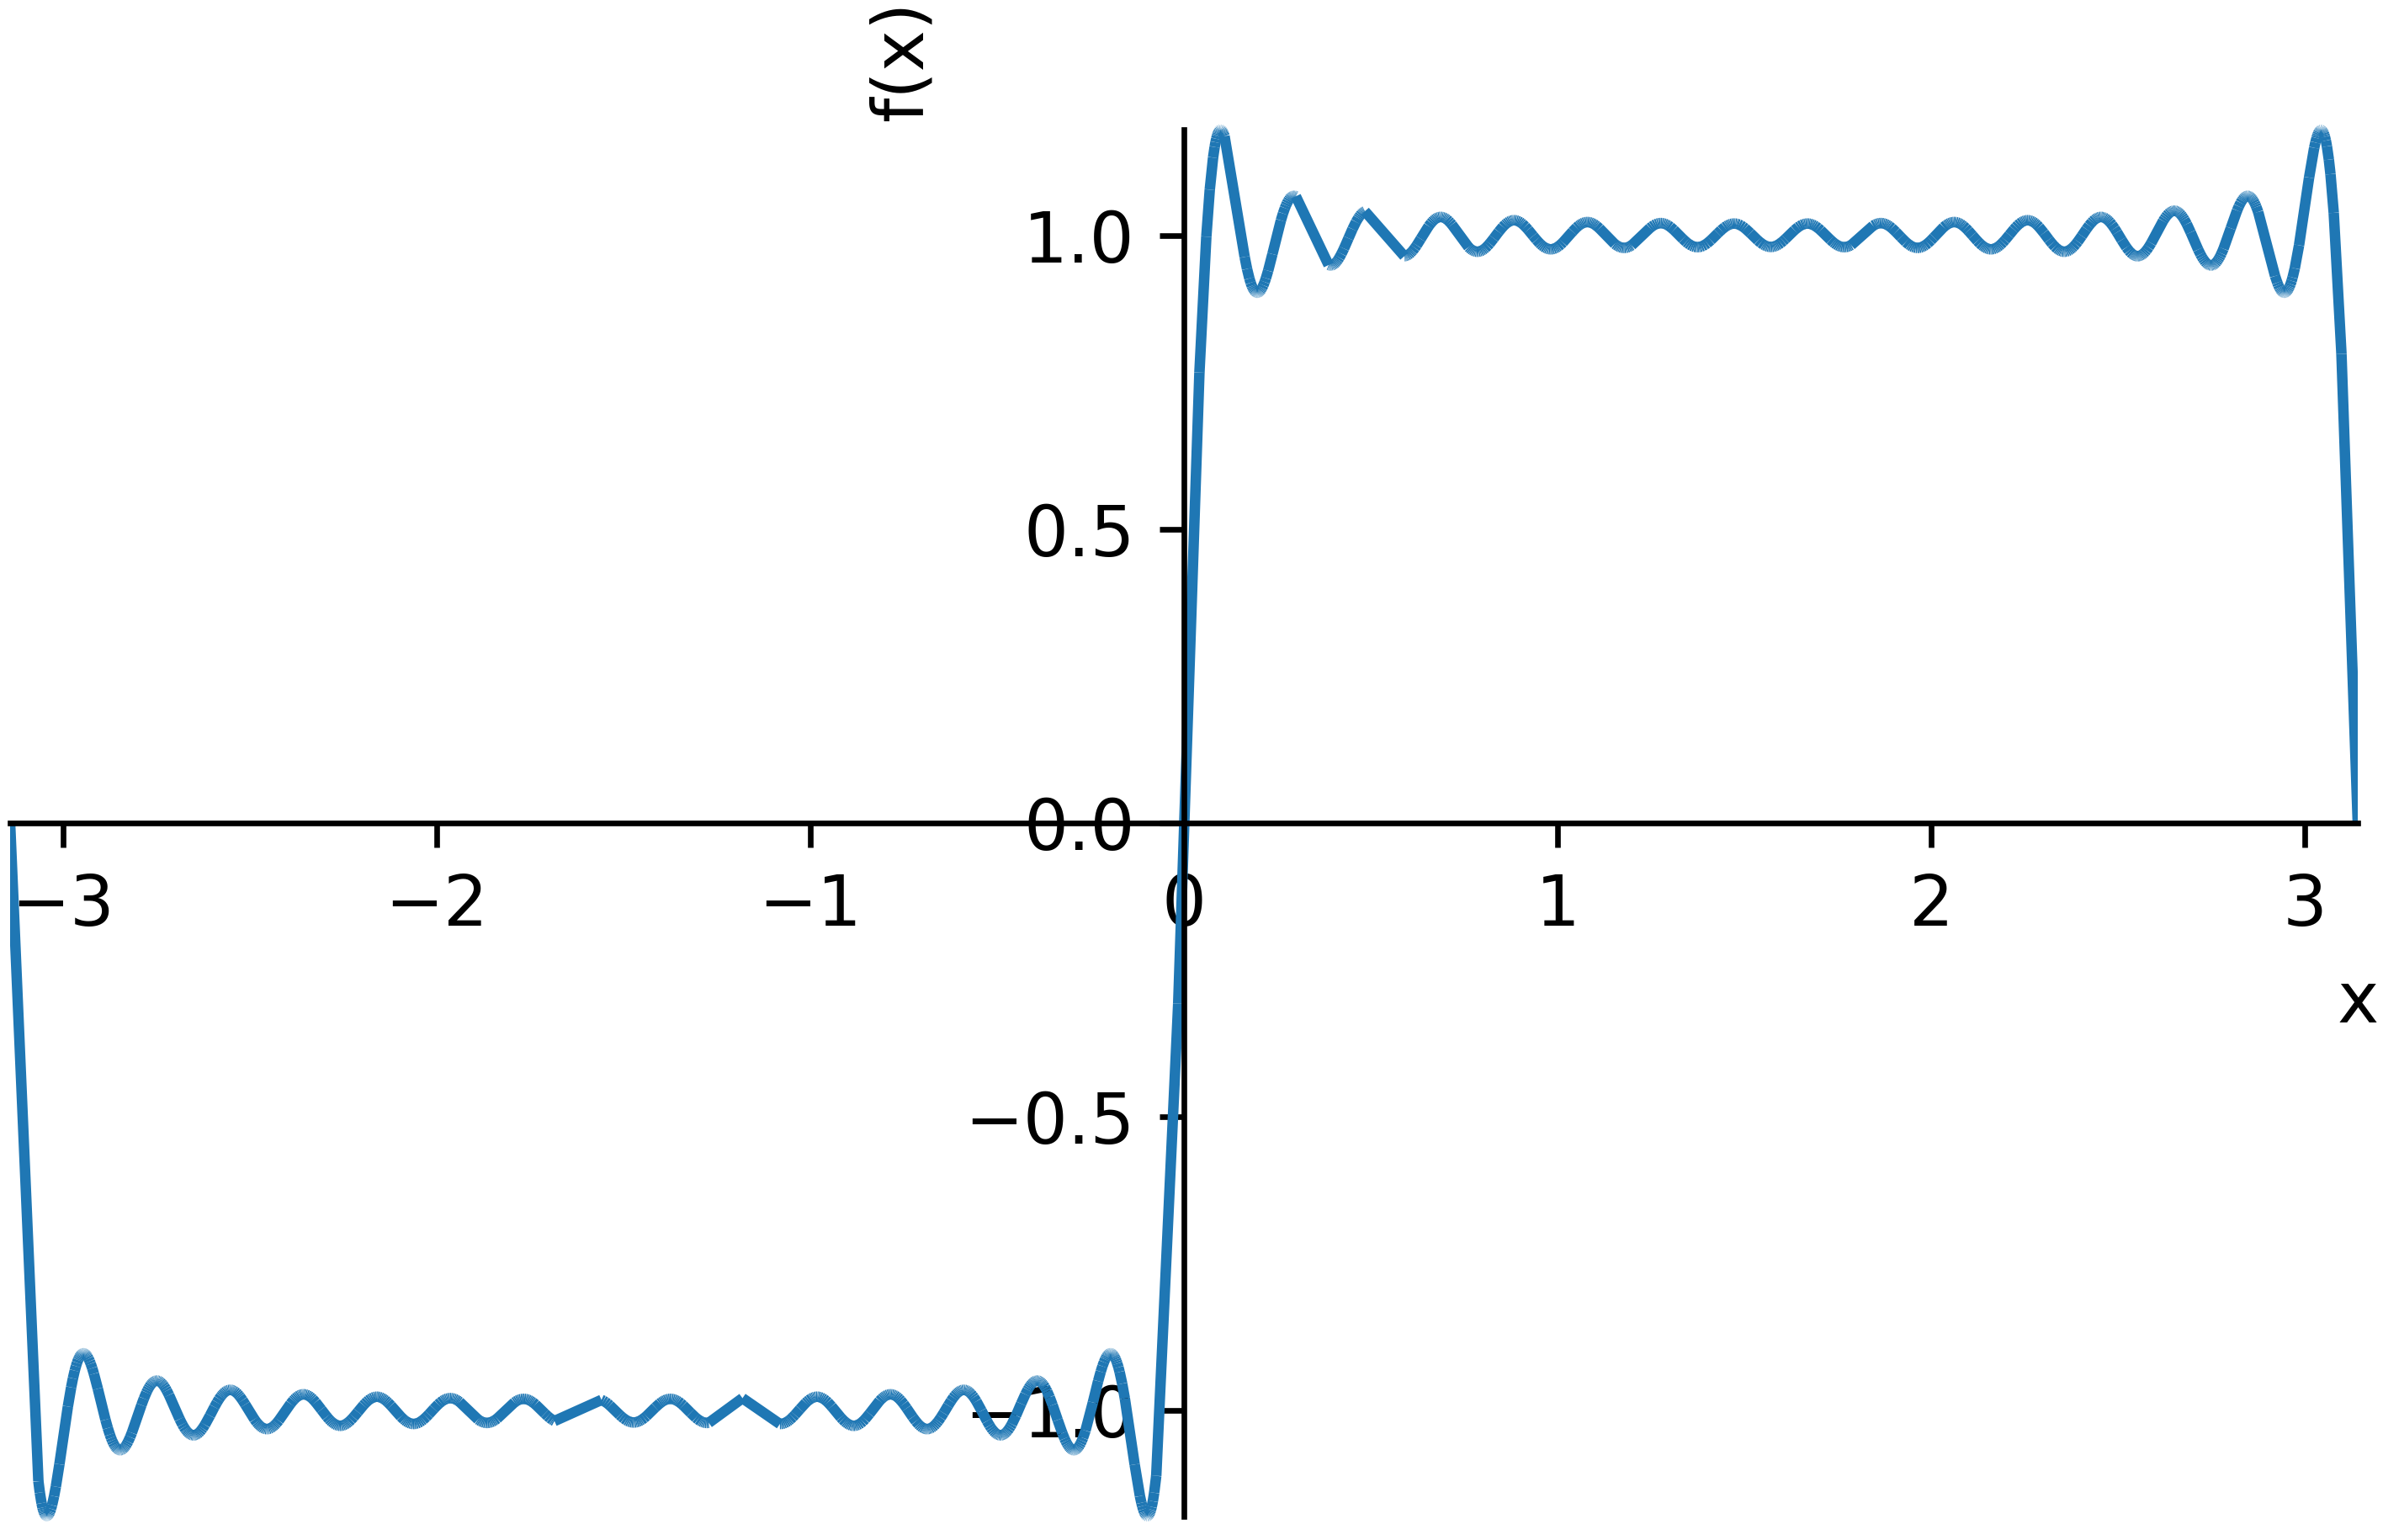
\includegraphics[height=5cm]{fourier.png}
  \end{center}
  \captionsetup{singlelinecheck=off}
  \caption{Lo sviluppo di Fourier della funzione
  che vale $1$ su $[0,\pi]$ e $-1$ su $[\pi,2\pi]$:
  $
  f_{61}(x)=
  \frac{4\sin(x)}{\pi} + \frac{4\sin(3x)}{3\pi} + \frac{4\sin(5x)}{5\pi} + \frac{4\sin(7x)}{7\pi} + \frac{4\sin(9x)}{9\pi} + \frac{4\sin(11x)}{11\pi} + \frac{4\sin(13x)}{13\pi} + \frac{4\sin(15x)}{15\pi} + \frac{4\sin(17x)}{17\pi} + \frac{4\sin(19x)}{19\pi} + \frac{4\sin(21x)}{21\pi} + \frac{4\sin(23x)}{23\pi} + \frac{4\sin(25x)}{25\pi} + \frac{4\sin(27x)}{27\pi} + \frac{4\sin(29x)}{29\pi} + \frac{4\sin(31x)}{31\pi}
  $.
  Il codice per calcolare i coefficienti e generare il grafico
  si trova a pagina~\pageref{code:Fourier}.
  Si può notare come nel punto di salto $x=\pi$ 
  lo sviluppo di Fourier ha una oscillazione maggiore del salto 
  originario (fenomeno di Gibbs).
  \index{Gibbs!fenomeno di}
  \index{fenomeno di Gibbs}
  L'incremento dell'oscillazione è circa del 9\% ed è indipendente 
  dal numero di termini utilizzati nello sviluppo di Fourier.
%  Significa che la serie di Fourier pur convergendo in norma $\Abs{\cdot}_2$
%  non converge uniformemente.
  }
  \label{fig:fourier}
  \end{figure}
    
Risulta naturale chiedersi se quella che abbiamo introdotto è una
\emph{base hilbertiana} perché solo in tal caso gli sviluppi di Fourier
approssimano la funzione.
Per ottenere questo risultato dobbiamo assumere la validità del seguente
teorema, che sarebbe ora troppo lungo dimostrare.

\begin{theorem}[densità dei polinomi trigonometrici]
Per ogni funzione continua $f\in C^0([0,2\pi])$
con $f(0)=f(2\pi)$ esiste una successione $g_k\in \H(0,2\pi)$ 
di polinomi trigonometrici
(cioè combinazioni lineari finite del sistema $\ENCLOSE{e_k}$)
tale che $g_k$ converge uniformemente a $f$.

In particolare l'insieme dei polinomi trigonometrici
è denso, con la norma uniforme,
nel sottospazio vettoriale
\[
  C^0_0([a,b]) 
  = \ENCLOSE{u\in C^0([a,b])\colon u(a)=u(b)=0}
  \subset C^0([a,b]).
\]
\end{theorem}

Osserviamo che la convergenza uniforme è più forte della convergenza
in $H(a,b)$ in quanto si ha, banalmente:
\[
  \Abs{f}_2^2 = \int_a^b f(x)^2\, dx
  \le \int_a^b \Abs{f}_\infty^2\, dx
  = (b-a) \cdot \Abs{f}_\infty^2.
\]
Dunque il teorema precedente garantisce che ogni funzione continua
in $\H(a,b)$ può essere approssimata, rispetto alla norma $\Abs{\cdot}_2$,
tramite polinomi trigonometrici. Il teorema seguente ci permette
di estendere questa proprietà a tutte le funzioni di $\H(a,b)$.

\begin{theorem}[densità delle funzioni continue]
Data una qualunque $f\in H(a, b)$ per ogni $\eps>0$
esiste una funzione continua $g\colon [a,b]\to \RR$
con $g(a)=g(b)=0$ tale che $\Abs{f-g}_2<\eps$.

Detto in altri termini: $C^0_0([a,b])=\ENCLOSE{u\in C^0\colon u(a)=u(b)=0}$ è un 
sottospazio denso in $H(a,b)$
cioè un insieme la cui chiusura (nella topologia di $H(a,b)$) 
è tutto $H(a,b)$.
\end{theorem}
%
\begin{proof}
\emph{Passo 1. Supponiamo che $f$ sia limitata su $(a,b)$.}
In tal caso possiamo pensare che $f$ sia definita su $[a,b]$
e l'integrale sia un integrale di Riemann ``proprio''.
Sia $M=\sup \abs{f}([a,b])$.
Per le condizioni di integrabilità sappiamo che per ogni $\eps>0$ è possibile
trovare una suddivisione $a=x_0 < x_1 < \dots < x_n =b$ su cui l'integrale
di $f$ differisce dagli integrali superiore e inferiore per meno di $\frac{\eps}{2M}$.
Possiamo prendere come funzione $g$ una interpolazione lineare
cioè una funzione tale che si abbia $g(x_k) = f(x_k)$ sui punti della suddivisione
e che risulti lineare su ogni intervallino $[x_k,x_{k+1}]$. La funzione
$g$ così definita è compresa, su ogni intervallino, tra l'$\inf$ e il $\sup$
di $f$ e dunque si avrà:
\[
 \int_a^b \abs{f(x)-g(x)}\, dx < \frac{\eps}{M}.
\]
Visto però che $\Abs{f}_\infty\le M$
si ha anche $\Abs{g}_\infty\le M$ e quindi $\Abs{f-g}_2\le 2M$.
Ma allora
\[
  \Abs{f-g}_2^2 = \int_a^b \abs{f-g}^2
  \le \int_a^b \Abs{f-g}_\infty \cdot \abs{f(x)-g(x)}\, dx
  \le 2M \frac{\eps}{2M} = \eps.
\]

\emph{Passo 2. Caso generale.}
Se la funzione è assolutamente 
integrabile in senso improprio su $(a,b)$ ma non è limitata, per
definizione di integrale improprio per ogni $\eps>0$ possiamo trovare un intervallo
$[\alpha,\beta]\subset (a,b)$
su cui $f^2$ (e quindi $f$) risulta limitata e
l'integrale di $f^2$ su $(a,\alpha]$ e su $[\beta,b)$
è minore di $\eps$. 
Sia $M=\sup \abs{f}([\alpha,\beta])$.
Applicando il passo precedente sull'intervallo $[\alpha,\beta]$ 
otteniamo una funzione continua $g$ definita su $[\alpha,\beta]$ 
tale che $\abs{g(x)}\le M$
e $\int\abs{f-g}^2\le \eps$.
L'idea è ora di prendere un punto $\alpha'\in(a,\alpha)$ 
e un punto $\beta'\in(\beta,b)$ ed estendere la funzione 
$g$ su tutto $[a,b]$ ponendo $g=0$ sugli intervalli 
$[a,\alpha']$ e $[\beta',b]$ e facendo una interpolazione 
lineare sugli intervalli $[\alpha',\alpha]$ e $[\beta,\beta']$.

Usando la disuguaglianza 
$(f-g)^2 \le (f-g)^2+(f+g)^2 = 2f^2+2g^2$
(si potrebbe altrimenti usare Cauchy-Schwarz due volte)
e scegliendo $\alpha'$ molto vicino ad 
$\alpha$ in modo che si abbia $\alpha-\alpha'<\eps/M^2$,
otteniamo
\[
  \int_a^\alpha \abs{f-g}^2 
  = \int_a^{\alpha'} f^2 + \int_{\alpha'}^\alpha \abs{f-g}^2
  \le \eps + 2\eps + 2M^2\cdot(\alpha-\alpha')
  \le 5\eps.
\]
Disuguaglianza analoga si avrà sull'intervallo $[\beta,b]$.
Dunque otteniamo in conclusione 
\[
\int_a^b \abs{f-g}^2
\le 5\eps + \eps + 5\eps  = 11 \eps
\]
e il teorema è dimostrato con $11\eps$ al posto di $\eps$.
\end{proof}

Grazie ai due teoremi precedenti sappiamo che ogni $f\in \H(a,b)$ può essere
approssimata da polinomi trigonometrici $g_N\to f$
cioè da funzioni della forma:
\[
  g_N = \sum_{k=0}^{N} a_{k,N} e_k.
\]
Stiamo qui assumendo che il polinomio trigonometrico $g_N$ abbia ordine non superiore
ad $N$, ma questo si può sempre assumere, scartando
o ripetendo i termini della successione.

Se ora consideriamo gli sviluppi di Fourier:
\begin{equation}\label{eq:48948784}
  f_N = \sum_{k=0}^N c_k e_k, \qquad c_k = \langle f,e_k\rangle
\end{equation}
ci ricordiamo che per ogni $k\le N$ risulta
\[
   \langle f-f_N, e_k \rangle
   = \sum_{k=0}^N \enclose{\langle f,e_k\rangle - c_k} = 0
\]
e quindi
\[
  \langle f-f_N , g_N -f_N\rangle
  = \sum_{k=0}^N \langle f-f_N, (a_{k,N}-c_k) e_k \rangle
  = 0.
\]
Dunque, applicando il teorema di Pitagora~\ref{th:spazio_euclideo},
\[
  \Abs{f-f_N}_2^2 = \Abs{f-g_N}_2^2 - \Abs{f_N-g_N}_2^2
  \le \Abs{f-g_N}_2^2 \to 0.
\]

Grazie al teorema~\ref{th:bessel} abbiamo quindi ottenuto il seguente.
\begin{theorem}[serie di Fourier]
Se $f\in \H(0,2\pi)$ e $c_k$, $f_N$
sono definiti da~\eqref{eq:48948784}
allora $f_k\to f$ in norma $\Abs{\cdot}_2$.
In particolare vale l'uguaglianza di Bessel
\begin{equation}\label{eq:uguaglianza_Bessel}
  \sum_{k=0}^{+\infty} c_k^2 = \Abs{f}_2^2.
\end{equation}
\end{theorem}


Questo significa, dunque, che il sistema ortonormale che abbiamo introdotto
è una base hilbertiana e quindi che ogni funzione $f\in \H(0,2\pi)$
si approssima
rispetto alla norma $\Abs{\cdot }_2$ con gli sviluppi di Fourier.

Ricordiamo che se $\Abs{f_N-f}_2 \to 0$ non è detto che si abbia la convergenza
puntuale $f_N(x)\to f(x)$ per ogni $x\in (0,2\pi)$ in quanto il limite è unico
in $H(a,b)$ ma non in $\H(a,b)$ e dunque è possibile (e in effetti può succedere)
che il limite puntuale degli sviluppi di Fourier differisca, in alcuni punti,
dalla funzione che si sta approssimando.

Purtroppo lo spazio $H(a,b)$ non risulta essere
completo, come si può vedere nel seguente esempio.

\begin{example}[razionali ingrassati]
\label{ex:incompletezza_di_H}%
Dimostriamo che lo spazio $H(0,1)$ non è completo.

Sappiamo che l'insieme $[0,1]\cap \QQ$ è numerabile, quindi esiste una
successione $q_k$ che elenca tutti i numeri razionali nell'intervallo $[0,1]$.
Poniamo inoltre $r_k = \frac{1}{4\cdot 2^k}$ e consideriamo gli intervalli
$I_k = [q_k-r_k,q_k+r_k]$.
Prendiamo la successione di funzioni $f_n\colon [0,1]\to \RR$
definita da
\[
  f_n(x) =
  \begin{cases}
  1 &\text{se } x\in\displaystyle\bigcup_{k=1}^{n} I_k\\
  0 & \text{altrimenti}
  \end{cases}
\]
A differenza di quanto uno potrebbe pensare, queste funzioni $f_n$ non diventano
mai identicamente uguali ad $1$. Anzi, si può osservare che
\[
  \int_0^1 f_n(x)\, dx
  \le \sum_{k=1}^n \int_{q_k-r_k}^{q_k+r_k} 1\, dx
  = \sum_{k=1}^n \frac{1}{2\cdot 2^k}
  \le \frac{1}{2}\sum_{k=1}^{+\infty}\frac{1}{2^k} = \frac 1 2.
\]

Si può mostrare che $f_k$ è una successione di Cauchy in $H(0,1)$ e
che però non converge in $H(0,1)$.
\end{example}

\begin{proof}
Per verificare che $f_n$ è una successione di Cauchy possiamo semplicemente
osservare che se $n\ge m$ risulta che $f_n$ e $f_m$ differiscono solamente
sugli intervalli $I_k$ con $k$ compreso tra $m$ ed $n$. Dunque:
\[
  \int_0^1 \abs{f_n - f_m}
  \le \sum_{k=m+1}^{+\infty} \int_{q_k-r_k}^{q_k+r_k} 1\,dx
  = \sum_{k=m+1}^{+\infty}\frac{1}{2\cdot 2^k} = \frac{1}{2^{m+1}}.
\]
Visto che $f_n$ e $f_m$ assumono solamente i valori $0$ e $1$ anche $\abs{f_n-f_m}$
assume solamente i valori $0$ e $1$ quindi $\abs{f_n-f_m}^2=\abs{f_n-f_m}$.
Abbiamo quindi verificato che per $n\ge m$ si ha:
\[
  \Abs{ f_n - f_m}_2 \le \sqrt{\frac{1}{2^{m+1}}}.
\]
E' dunque chiaro che comunque sia scelto $\eps>0$ possiamo scegliere $N$
tale che $1/2^N \le \eps^2$ da cui si ottiene che se $n,m\ge N$
allora $\Abs{f_n-f_m}_2 \le \eps$. Cioè: $f_n$ è una successione di Cauchy.

Supponiamo ora, per assurdo, che esista $f\in H(0,1)$
tale che $\Abs{f_n-f}_2 \to 0$.
Innanzitutto visto che ogni $f_k\le 1$ possiamo supporre che sia anche $f\le 1$
perché altrimenti potremmo prendere $g(x) = \min\ENCLOSE{f(x),1}$ e avremmo
chiaramente $\Abs{f_n - g}_2 \le \Abs{f_n -f}_2 \to 0$. In pratica stiamo dicendo
che modificando la funzione $f$ senza cambiarne l'integrale possiamo suppore
che $f(x)\le 1$ per ogni $x\in[0,1]$.

Fissato un intervallo $I_n$, per $k\to +\infty$ si ha:
\[
  0\le \int_{q_n-r_n}^{q_n+r_n}\abs{f_k(x)-f(x)}^2\, dx
  \le \int_0^1 \abs{f_k(x)-f(x)}^2\, dx = \Abs{ f_k -f}_2^2 \to 0.
\]
Ma ora se $k\ge n$ risulta che $f_k=1$ su $I_n$ e quindi il valore dell'integrale
precedente non dipende da $k$ e dovrà quindi essere identicamente nullo:
\[
  \int_{q_n-r_n}^{q_n+r_n} (1-f(x)) \, dx = 0
\]
e quindi possiamo affermare che $\sup f(I_n) = 1$ in quanto se fosse
$\sup f(I_n) = \lambda < 1$
l'integrale di $1-f(x)$ sarebbe positivo
sull'intervallo $I_n$.

Vogliamo ora dimostrare che su ogni intervallo $[a,b]\subset[0,1]$, se $b>a$
si ha $\sup f([a,b])=1$. 
Prendiamo $N$ abbastanza grande in modo che $r_N < (b-a)/3$.
Allora l'intervallo $[a+r_N, b-r_N]$ ha ampiezza maggiore di $r_N$ e contiene infiniti
numeri razionali. 
Esistono quindi infiniti indici $n$ per cui $q_n$ sta in tale
intervallo. 
Tra questi infiniti certamente ce n'è uno con indice $n\ge N$
(perché i $q_n$ con $n<N$ sono in numero finito). 
Ma se $q_n \in [a+r_N,b-r_N]$
allora $I_n\subset[a,b]$ e quindi $\sup f([a,b])\ge \sup f(I_n) = 1$.

Questo significa che per ogni suddivisione di Riemann dell'intervallo $[0,1]$
risulta che il $\sup$ di $f$ sugli intervallini della suddivisione è $1$ e quindi
l'integrale superiore di $f$ è anch'esso $1$. 
Dunque, essendo $f$ integrabile,
\[
  \int_a^b f(x) = 1.
\]

Vogliamo ora concludere che questo è in contraddizione con la disuguaglianza
\[
  \int_a^b f_n(x) \le \frac 1 2
\]
che abbiamo osservato all'inizio.
Si ha infatti per la disuguaglianza di Cauchy-Schwarz
\begin{align*}
  \int_0^1 \abs{f(x)-f_n(x)}\, dx
  \le \Abs{f-f_n}_2\cdot \Abs{1}_2  \to 0
\end{align*}
e quindi, per il criterio di convergenza assoluta,
\[
  \int_0^1 (f(x) - f_n(x))\, dx \to 0.
\]
Ma abbiamo visto che
\[
  \int_0^1 (f(x) - f_n(x))\, dx
  = \int_0^1 f(x)\, dx - \int_0^1 f_n(x)\, dx
  \ge 1 - \frac 1 2 = \frac 1 2
\]
ottenendo quindi un assurdo.
\end{proof}

Il fatto di avere trovato una base hilbertiana di $H(0,2\pi)$ (e quindi
di ogni $H(a,b)$) ci permette di
dire che ogni funzione in $H(0,2\pi)$ può essere rappresentata dalle sue
coordinate $c_k$ in modo che valga l'uguaglianza di Bessel:
\[
  \Abs{f}_2 = \sqrt{\sum_{k=0}^{+\infty} c_k^2}.
\]
Abbiamo in effetti definito una corrispondenza:
\[
  \phi \colon H(0,2\pi) \to \ell^2,
  \qquad
  \ell^2=\ENCLOSE{c\in \RR^\NN \colon \sum_{k=0}^{+\infty} c_k^2<+\infty}
\]
definita da
\[
  c_k = \phi(f) = \langle f, e_k\rangle.
\]
Chiaramente tale $\phi$ è lineare. Visto che $e_k$ è una base hilbertiana
è facile verificare che $\phi$ è anche iniettivo. Se su $\ell^2$
definiamo il prodotto scalare e la norma corrispondente:
\[
  \langle x,y\rangle = \sum_{k=0}^{+\infty} x_k y_k, \qquad
  \abs{x}_2 = \sqrt{\sum_{k=0}^{+\infty}} x_k^2
\]
l'uguaglianza di Bessel ci dice che $\phi$ mantiene la norma e quindi
la struttura di spazio euclideo. Si potrebbe dimostrare che $\ell^2$
è completo e questo significa che $\phi$ non è suriettiva in quanto
la successione $f_n$
considerata nell'esempio~\ref{ex:incompletezza_di_H}
è di Cauchy in $H(0,2\pi)$, dunque $\phi(f_n)$ è di Cauchy in $\ell^2$
e dunque converge in $\ell^2$. Il limite $c$ della successione $\phi(f_n)$
rappresenta una successione di coefficienti di Fourier che non possono
essere ottenuti da nessuna funzione $f\in H(0,2\pi)$.

Possiamo utilizzare le serie di Fourier per risolvere 
il seguente\mynote{vedi note storiche a pag~\pageref{note:Basilea}}.

\begin{exercise}[problema di Basilea]
\label{ex:Basilea}%
Dimostriamo che
\begin{equation}\label{eq:basilea}
  \sum_{k=1}^{+\infty} \frac{1}{k^2} = \frac{\pi^2}{6}.
\end{equation}
\end{exercise}
%%
%%
\begin{proof}[Svolgimento.]
Calcoliamo i coefficienti di Fourier della funzione $f(x)=x$ in $H(0,2\pi)$.
Si ha
\[
 c_0 = \int_0^{2\pi} f(x)\cdot e_0(x)\, dx = \int_0^{2\pi} \frac{x}{\sqrt{2\pi}}\, dx = \frac{1}{\sqrt{2\pi}}\Enclose{\frac{x^2}{2}}_0^{2\pi}
  = \sqrt{2\pi^3}
\]
poi
\begin{align*}
  c_{2k+1} &= \int_0^{2\pi} x \cdot \frac{\sin(kx)}{\sqrt \pi}\, dx \\
   &= \Enclose{\frac{x(-\cos(kx))}{k\sqrt \pi}}_0^{2\pi}
   - \int_0^{2\pi} \frac{-\cos(kx)}{k\sqrt \pi}\, dx\\
   &= \frac{-2\pi}{k\sqrt \pi} - 0 = -\frac{2\sqrt \pi}{k}
\end{align*}
e infine
\begin{align*}
  c_{2k} &= \int_0^{2\pi} x \cdot \frac{\cos (kx)}{\sqrt \pi}\, dx \\
  &= \Enclose{\frac{x \sin(kx)}{\sqrt \pi k}}_0^{2\pi}
  - \int_0^{2\pi} \frac{\sin(kx)}{\sqrt \pi k}\, dx
  = 0.
\end{align*}
Allora l'equazione di Bessel~\eqref{eq:uguaglianza_Bessel} ci dice
che vale
\[
  \Abs{x}_2^2 = \sum_{k=0}^{+\infty} c_k^2
  = c_0^2 + \sum_{k=0}^{+\infty} c_{2k+1}^2
  = 2\pi^3 + \sum_{k=1}^{+\infty} \frac{4\pi}{k^2}.
\]
Ma è facile calcolare
\[
 \Abs{x}_2^2 = \int_0^{2\pi} x^2\, dx = \Enclose{\frac{x^3}{3}}_0^{2\pi}
  = \frac{8\pi^3}{3}
\]
e quindi
\[
  \frac{8\pi^3}{3} = 2\pi^3 + 4\pi \sum_{k=1}^{+\infty}\frac{1}{k^2}
\]
da cui segue il risultato voluto.
\end{proof}


\section{divagazione sui frattali autosimili}

In questo capitolo mostriamo una applicazione geometrica del teorema delle contrazioni.
Considereremo uno spazio metrico i cui punti sono le figure geometriche
e vedremo che i frattali autosimili non sono altro che punti fissi
di opportune mappe contrattive.

\begin{definition}
Siano $A$ e $B$ sottoinsiemi non vuoti di $\RR^n$.
Definiamo la \emph{distanza di Hausdorff}
\mymargin{distanza di Hausdorff}
\index{distanza!di Hausdorff}
tra $A$ e $B$ come:
\[
  d_{\H}(A,B) = \max\ENCLOSE{\sup_{a\in A}\inf_{b\in B} \abs{a-b}, \sup_{b\in B} \inf_{a\in A} \abs{a-b}}.
\]

Definiamo
\[
 \K(\RR^n) = \ENCLOSE{A \subset \RR^n \colon \text{$A$ chiuso, limitato, non vuoto}}.
\]
\end{definition}

\begin{theorem}[caratterizzazione della distanza di Hausdorff]
Se $A$ e $B$ sono compatti di $\RR^n$ (cioè chiusi e limitati) allora
per ogni $r \in \RR$
si ha
\[
  d_\H(A,B) \le r
\]
se e solo se valgono entrambe le seguenti proprietà:
\begin{enumerate}
\item per ogni $a\in A$ esiste $b\in B$ tale che $\abs{a-b}\le r$;
\item per ogni $b\in B$ esiste $a\in A$ tale che $\abs{a-b}\le r$.
\end{enumerate}
\end{theorem}
%
\begin{proof}
Per ogni compatto non vuoto $A$ e per ogni $x\in \RR^n$ definiamo
la distanza tra il punto $x$ e l'insieme $A$ come:
\[
  d(x,A) = \min_{a\in A} \abs{x-a}.
\]
Il minimo esiste in quanto $A$ è compatto e $a\mapsto d(x,a)$ è una funzione continua. Fissato $A$ la funzione $x\mapsto d(x,A)$ è anch'essa continua, anzi è $1$-lipschitziana. Infatti se $x'\in \RR^n$ esiste $a'\in A$ tale che $d(x',A) = d(x',a')$ e dunque
\[
  d(x,A) = \min_{x\in A} \abs{x-a} \le \abs{x-a'} \le \abs{x-x'} + \abs{x'- a'}
   = \abs{x-x'} + d(x',A)
\]
da cui $d(x,A) - d(x',A)\le \abs{x-x'}$.
Scambiando $x$ e $x'$ si ottiene anche la disuguaglianza inversa da cui la $1$-lipschitzianità di $d(x,A)$. Dunque sui compatti la funzione $d(x,A)$ assume sempre massimo e si ha:
\[
d_\H(A,B) = \max\ENCLOSE{\max_{a_\in A} d(a,B), \max_{b\in B} d(b,A)}.
\]

In particolare se $d_\H(A,B) \le r$ per ogni $a\in A$ si deve avere $d(a,B) \le r$ e per ogni $b\in B$ si deve avere $d(b,A) \le r$. Ma allora valgono le due proprietà dell'enunciato.

Viceversa se vale la proprietà 1.\ allora $d(a,B)\le r$ e se vale la 2.\ $d(b,A)\le r$ e di conseguenza $D_\H(A,B) \le r$.
\end{proof}

\begin{theorem}[distanza di Hausdorff]
La distanza di Hausdorff $d_\H$ è una distanza su $\K(\RR^n)$ e lo spazio metrico $\K(\RR^n)$ è completo.
\end{theorem}
%
\begin{proof}
Chiaramente se $A,B$ sono non vuoti si ha $d_\H(A,B) \ge 0$.
Inoltre, in base alla caratterizzazione del teorema precedente è facile osservare che $d_\H(A,B) < +\infty$.

Se $d_\H(A,B) = 0$ significa che per ogni $a\in A$ esiste $b\in B$ tale che $\abs{a-b}=0$. Cioè $b=a$. Dunque $A\subset B$. Scambiando i ruoli di $A$ e $B$ si ottiene anche $B\subset A$ da cui $A=B$.

Che sia $d_\H(A,B) = d_\H(B,A)$ è ovvio in quanto la definizione è simmetrica in $A$ e $B$.

Verifichiamo ora la disuguaglianza triangolare. Siano $A,B,C$ tre compatti non vuoti. Per ogni $a\in A$ esiste $b\in B$ tale che $\abs{a-b} \le d_\H(A,B)$ e per tale $b \in B$ esiste un $c\in C$ tale che $\abs{b-c} \le d_\H(B,C)$. Dunque per ogni $a\in A$ esiste un $c\in C$ tale che
\[
  \abs{a-c} \le \abs{a-b} + \abs{b-c} \le d_\H(A,B) + d_\H(B,C).
\]
Scambiando i ruoli di $A$ e $C$ si ottiene anche la condizione simmetrica e dunque, per la caratterizzazione della distanza di Hausdorff si ottiene la disuguaglianza triangolare:
\[
  d_\H(A,C) \le d_\H(A,B) + d_\H(B,C).
\]

Abbiamo quindi verificato che $d_\H$ è una distanza su $\K(\RR^n)$. Verifichiamo ora che $\K(\RR^n)$ è completo.

Sia $A_k\in\K(\RR^n)$ una successione di Cauchy.
Senza perdita di generalità possiamo supporre che
\[
  d_\H(A_k,A_{k+1}) \le \frac{1}{2^k}.
\]
Infatti essendo $A_k$ di Cauchy è possibile trovarne una sottosuccessione con tale proprietà, e se poi dimostriamo che la sottosuccessione converge allora l'intera successione, essendo di Cauchy, deve convergere.

Consideriamo come candidato limite l'insieme di tutti i possibili limiti di punti degli insiemi $A_k$:
\[
  A = \ENCLOSE{x\in \RR^n
  \colon \exists x_k \in A_k\colon x_k \to x}.
\]

Per prima cosa vogliamo verificare che $A$ non è vuoto. Scelto un punto qualunque $a_0 \in A_0$ esiste $a_1 \in A_1$ tale che $\abs{a_0 - a_1} = d_\H(A_0,A_1)$. Iterando otteniamo una successione di punti $a_k \in A_k$ tale che $\abs{a_k - a_{k+1}} \le d_\H(A_k,A_{k+1}) \le 1/2^k$.
Dunque $a_k$ è una successione di Cauchy in $\RR^n$ ed essendo $\RR^n$ completo dovrà convergere ad un punto $a$ che quindi è un punto di $A$.

Avendo assunto $d_\H(A_k, A_{k+1}) < 1/2^k$ si ottiene (sommando la serie geometrica):
\[
 d_\H(A_k, A_n) \le \sum_{j=k}^{n-1} d_\H(A_j, A_{j+1}) \le \frac{2}{2^k}\qquad \text{se $n>k$}.
\]
Questo ci permette di dimostrare che per ogni $a\in A$ e per ogni $k\in \NN$ esiste $a_k \in A_k$ tale che
$\abs{a - a_k}\le 4/2^k$. Infatti se a distanza $4/2^k$ non ci fossero punti di $A_k$ allora a distanza $2/2^k$ non ci potrebbero essere punti di $A_n$ per nessun $n>k$ in quanto visto che $d_\H(A_k,A_n) \le 2/2^k$ se ci fosse un punto di $A_n$ a distanza inferiore a $2/2^k$ ci dovrebbe anche essere un punto di $A_k$ a distanza inferiore a $4/2^k$. Ma questo è impossibile perché per come è definito $A$ deve esistere $x_n \in A_n$ tale che $x_n \to a$. Abbiamo quindi mostrato che
\[
  \sup_{a\in A} \inf_{b\in A_k} \abs{a-b} \le 4/2^k \to 0.
\]

Viceversa ci proponiamo di mostrare che per ogni $p \in A_k$ esiste $a \in A$ tale che $\abs{p-a} < 2/2^k$.
Visto che $d_\H(A_{j+1},A_j) \le 1/2^j$
possiamo infatti costruire a partire da $a_k=p \in A_k$
una successione $a_j \in A_j$ con $j > k$, tale che $d(a_{j+1},a_j) \le 1/2^j$. Tale successione è di Cauchy
quindi converge: $a_j \to a$
e il suo limite $a$ è quindi un punto di $A$ e si ha
\[
  \abs{a-p} \le \sum_{j=k}^\infty \abs{a_j - a_{j+1}}
    \le \sum_{j=k}^\infty \frac{1}{2^j} \le \frac{2}{2^k}.
\]
Abbiamo quindi dimostrato che
\[
  \sup_{b\in a_k} \inf_{a\in A} \abs{a-b} \le 2/2^k \to 0
\]
e quindi $d_\H(A_k,A)\to 0$.

Ci rimane solo da mostrare che $A$ è un insieme chiuso.
Presa una successione di punti $x_k\in A$ convergente $x_k\to x$, dobbiamo mostrare che $x\in A$. Per ogni $x_k\in A$ per quanto già detto sappiamo esistere $a_k \in A_k$ tale che $\abs{a_k-x_k}\le 4/2^k$. Ma allora $\abs{a_k-a} \le 4/2^k + \abs{x_k-a} \to 0$ e quindi $a_k\to a$ da cui $a\in A$.
 \end{proof}

\begin{theorem}[frattali autosimilari]
Siano $\phi_1, \dots, \phi_N \colon \RR^n \to \RR^n$ contrazioni (cioè funzioni lipschitziane con costante di lipschitz inferiore ad $1$).
Allora
esiste un unico insieme $C\subset \RR^n$ chiuso e limitato tale che
\[
  C = \bigcup_{k=1}^N \phi_k(C).
\]
\end{theorem}
%
\begin{proof}
Basterà dimostrare che la funzione $T\colon \K(\RR^n)\to \K(\RR^n)$ definita da
\[
  T(A) = \bigcup_{k=1}^N \phi_k(C)
\]
è una contrazione: dopodiché sapendo che $\K(\RR^n)$ è completo il risultato è conseguenza diretta del teorema di punto fisso di Banach-Caccioppoli.

Ogni $\phi_k$ per ipotesi è una contrazione, cioè
per ogni $a,b\in X$
\[
  \abs{\phi_k(a)-\phi_k(b)} \le L_k \abs{a-b}
\]
con $L_k< 1$. Posto $L=\max \ENCLOSE{L_1, \dots, L_N} < 1$ vogliamo dimostrare che $T$ è $L$-lipschitziana (e dunque una contrazione). Siano $A,B \in \K(\RR^n)$ e sia $d = d_\H(A,B)$. Preso $a' \in T(A)$ dovrà esistere $k$ tale che $a' \in \phi_k(A)$. Cioè $a'= \phi_k(a)$ con $a\in A$. Ma allora esiste $b\in B$ con $\abs{a-b}\le d_\H(A,B) = d$ e quindi $b'=\phi_k(b) \in T(B)$ e $\abs{a'-b'} = \abs{\phi_k(a)-\phi_k(b)} \le L \abs{a-b} \le L \cdot d$. Dunque abbiamo mostrato che
\[
  \sup_{a' \in T(A)} \inf_{b'\in T(B)} \abs{a'-b'} \le L d_\H(A,B).
\]
La stessa disuguaglianza rimane valida con $A$ e $B$ scambiati, ottenendo quindi:
\[
  d_\H(T(A),T(B)) \le L\cdot d_\H(A,B).
\]
\end{proof}

\begin{example}[insieme di Cantor]
  \label{ex:insieme_Cantor}%
Si prendano $\phi, \psi\colon \RR \to \RR$ definite da
\[
  \phi(x) = \frac{x}{3}, \qquad
  \psi(x) = \frac{2+x}{3}.
\]
Chiaramente $\phi$ e $\psi$ sono $1/3$-lipschitziane e dunque, per il teorema precedente, esiste un unico insieme $C$ chiuso e limitato in $\RR$ tale che
\[
  C = \frac{C}{3} \cup \frac{C+2}{3}.
\]
Tale insieme si chiama \emph{insieme di Cantor}%
\mymargin{insieme di Cantor}\index{insieme!di Cantor}.
\index{Cantor!insieme di}

L'insieme di Cantor è un frattale autosimile in quanto si ottiene come l'unione di due copie riscalate di sé stesso.

E' facile mostrare che $C\subset [0,1]$ in quanto $T$ manda sottoinsiemi di $[0,1]$ in sottoinsiemi di $[0,1]$.
Ogni $x\in [0,1]$ può essere rappresentato in base $3$ con una sequenza di cifre ternarie: $0,1,2$. La funzione $\phi(x)$ aggiunge uno $0$ in cima alla sequenza di cifre, mentre la funzione $\psi(x)$ aggiunge un $2$ in cima alla sequenza.
Vogliamo mostrare che $C$ è l'insieme di tutti i numeri in $[0,1]$ che possono essere scritti in base $3$ utilizzando solamente le cifre $0$ e $2$. Osserviamo innanzitutto che $C$ è chiuso: il suo complementare in $[0,1]$ è formato da tutti i numeri che in base $3$ si devono scrivere utilizzando almeno una cifra $1$. Ma se c'è una cifra $1$ posso modificare tutte le cifre successive rimanendo nel complementare di $C$: dunque il complementare di $C$ è aperto. Si osservi che gli unici numeri che hanno una doppia rappresentazione in base $3$ sono quelli che terminano con una sequenza infinita di $2$,
\end{example}

\begin{figure}
\centering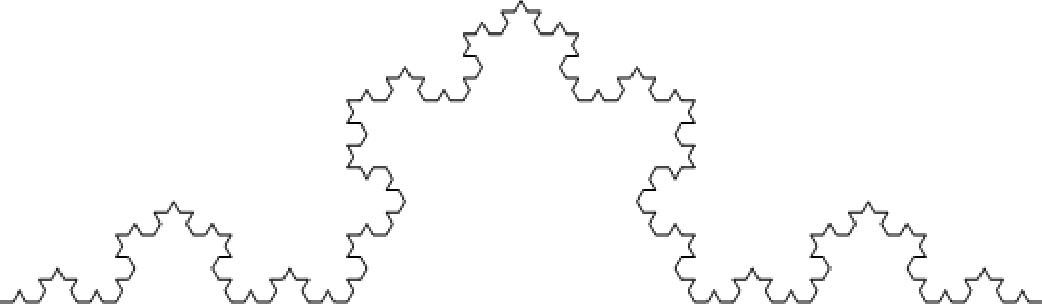
\includegraphics[width=1.0\textwidth]{koch_picture}
\caption{
Chiamato $K_0 \in \RR^2$ il segmento $[0,1]\times \ENCLOSE{0}$,
in figura è rappresentata
la quarta iterata $K_4 = T^4(K_0)$ della contrazione che definisce la curva di K{\"o}ch.
A pagina~\pageref{code:Koch} il codice per generare la figura.
\index{curva di K{\"o}ch}%
}
\label{fig:koch}
\end{figure}

\begin{example}[curva di K{\"o}ch]
Sia $R_\theta\colon \RR^2 \to \RR^2$ la rotazione con centro l'origine di $\theta$ radianti in senso antiorario.
Sia $\alpha = \pi/3$, $p=(1,0)$ e
siano $\phi_1, \phi_2, \phi_3, \phi_4 \colon \RR^2 \to \RR^2$
le funzioni definite da:
\begin{align*}
\phi_1(v) = \frac{v}{3}, \qquad
\phi_2(v) = R_{\alpha}\frac{v}{3} + \phi_1(p), \\
\phi_3(v) = R_{-\alpha}\frac{v}{3} + \phi_2(p), \qquad
\phi_4(v) = \frac{v}{3} + \phi_3(p).
\end{align*}
Allora esiste un unico insieme chiuso $K\subset \RR^2$ tale che
\[
  K = \phi_1(K) \cup \phi_2(K) \cup \phi_3(K) \cup \phi_4(K).
\]
L'insieme $K$ si chiama \emph{curva di K{\"o}ch}%
\mymargin{curva di K{\"o}ch}%
\index{curva di K{\"o}ch}. 
E' un frattale autosimile in quanto è composto da quattro copie riscalate di se stesso.
\end{example}


\section{note storiche}

\label{note:Basilea}%
Il problema di Basilea è un problema posto da Mengoli nel 1650 
e risolto da Eulero nel 1734 dopo che i maggiori matematici del tempo 
(tra cui i famosi membri della famiglia Bernoulli che vivevano appunto a Basilea) 
avevano tentato invano di risolverlo. 
Si tratta di determinare la somma della serie \eqref{eq:basilea}.
La soluzione di Eulero (completamente diversa da quella che stiamo proponendo qui)
è stata poi ripresa da Riemann che ha definito la celebre funzione \emph{zeta}
\index{Riemann!funzione $\zeta$}%
\index{$\zeta$!di Riemann}%
\index{Basilea!problema di}%
\index{problema!di Basilea}%
\index{Eulero!problema di Basilea}%
\index{$\pi$!problema di Basilea}%
\[
\zeta(s) = \sum_{k=1}^{+\infty} \frac{1}{k^s}  
\]
di grandissima rilevanza nella teoria dei numeri.



\chapter{successioni ricorsive}
\label{ch:successioni_ricorsive}

Nella maggior parte di questo capitolo prenderemo in considerazione le successioni $a_n$
definite \emph{per ricorrenza} o \emph{ricorsivamente} dalle condizioni:
\index{successione!ricorsiva}
\index{successione!definita per ricorrenza}
\index{ricorsione}
\begin{equation}\label{eq1}
\begin{cases}
  a_0 = \alpha,\\
  a_{n+1} = f(a_n)
\end{cases}
\end{equation}

Fissato il termine iniziale $\alpha$ e la legge di ricorrenza $f$,
c'è una unica successione che soddisfa \eqref{eq1} e i suoi termini
sono:
\begin{align*}
a_0 & =\alpha,\\
a_1 &= f(a_0)=f(\alpha),\\
a_2 &= f(a_1)=f(f(\alpha)),\\
a_3 &= f(a_2)=f(f(f(\alpha))),\\
&\ \vdots\\
a_n &= f(a_{n-1}) = f^n(\alpha),\\
&\ \vdots
\end{align*}


Il valore di $a_n$ potrebbe rappresentare lo stato di un sistema che
si evolve a partire da uno stato iniziale $a_0=\alpha$ tramite la
funzione $f$ che rappresenta il cambiamento di stato.
Il numero naturale $n$ potrebbe quindi rappresentare un passo temporale.
In tal senso \eqref{eq1} si chiama anche \emph{sistema dinamico discreto}%
\mymargin{sistema dinamico discreto}\index{sistema!dinamico!discreto}.

L'equazione $a_{n+1} = f(a_n)$ viene chiamata una \emph{equazione ricorsiva autonoma del primo ordine}.
Ci sono altre tipologie di equazioni che considereremo
solo marginalmente nei capitoli successivi.
Ad esempio quando abbiamo definito
il fattoriale: $a_n = n!$ abbiamo dato le condizioni:
\[
\begin{cases}
  a_0 = 1\\
  a_{n+1} = (n+1) \cdot a_n
\end{cases}
\]
ma l'equazione $a_{n+1} = (n+1) \cdot a_n$ è della forma $a_{n+1} =
f(n, a_n)$ e si dice essere \emph{non autonoma} perché la funzione di
ricorrenza $f$ dipende esplicitamente da $n$ oltre che dal termine
precedente $a_n$.

Si potrebbero anche considerare equazioni di ordine maggiore del
primo. Ad esempio la successione $F_n$ di \emph{Fibonacci}
(Leonardo Pisano, 1170--1242)
i cui primi termini sono riportati nella tabella~\ref{tab:Fibonacci}
\begin{table}
  \begin{center}
  0, 1, 1, 2, 3, 5, 8, 13, 21, 34, 55, 89, 144,
  233, 377, 610, 987\dots
\end{center}
\caption{I primi termini della succession di Fibonacci.
Ogni termine è la somma dei due precedenti.}
\label{tab:Fibonacci}
\end{table}
\mymargin{Fibonacci}%
\index{Fibonacci}%
\index{Fibonacci!successione di}%
\index{successione!di Fibonacci}%
soddisfa l'equazione ricorsiva:
\begin{equation}\label{eq:Fibonacci}
\begin{cases}
  F_0 = 0 \\
  F_1 = 1 \\
  F_{n+2} = F_{n+1} + F_n
\end{cases}
\end{equation}
che è una relazione del secondo ordine in quanto ogni termine può
essere definito utilizzando i valori dei \emph{due} termini precedenti.
Se l'equazione è lineare, come in questo caso, si possono trovare delle
formule esplicite per scrivere l'$n$-esimo termine della successione.
Lo faremo nella sezione~\ref{sec:ricorrenza_lineare}

Si potrebbero anche considerare i sistemi di equazioni ricorsive.
Ad esempio se $f$ fosse una funzione complessa $f\colon \CC \to \CC$,
$f(x+iy) = f_1(x,y) + i f_2(x,y)$ con $f_1,f_2 \colon \RR\times\RR\to\RR$
si potrebbe scrivere $a_n = x_n + i y_n$ con $x_n, y_n \in \RR$
e l'equazione ricorsiva $a_{n+1} = f(a_n)$
diventerebbe un sistema di due equazioni:
\[
  \begin{cases}
    x_{n+1} = f_1(x_n, y_n)\\
    y_{n+1} = f_2(x_n, y_n).
  \end{cases}
\]
Lo studio dei sistemi va oltre gli scopi di questo capitolo,
ma accenneremo solamente ad un esempio nella sezione~\ref{sec:mandelbrot}.


\section{equazioni ricorsive autonome del primo ordine}

\begin{example}[algoritmo di Erone]\label{ex_Erone}
\index{Erone!algoritmo di}%
\index{algoritmo!di Erone}%
\index{algoritmo!calcolo della radice $n$-esima}%
\index{radice $n$-esima!algoritmo di Erone}%
  Fissato un numero reale $p>1$ consideriamo la successione definita
  per
ricorrenza da
\[
\begin{cases}
  a_0 = p\\
  a_{n+1} = \frac{a_n + p/a_n}{2}.
\end{cases}
\]
Si dimostri che $a_n \to \sqrt p$.
\end{example}
Osserviamo, ad esempio, che per $p=2$ i
primi termini della successione sono:
\begin{align*}
a_0 &= 2, \\
a_1 &= \frac{2+2/2}{2} = 3/2 = 1.5, \\
a_2 &= \frac{3/2 + 2/(3/2)}{2} = 17/12 \approx 1.4166666, \\
a_3 &= \frac{17/12 + 2/(17/12)}{2} = 577 / 408 \approx 1.4142157,\\
\vdots
\end{align*}
che effettivamente \emph{sembrano} avvicinarsi molto al numero
\[
\sqrt 2\approx 1.4142135.
\]

\begin{proof}
\emph{Passo 1.} Dimostriamo per induzione che $a_n>0$ per ogni $n\in \NN$.
Infatti per $n=0$ osserviamo che $a_0=p>0$ mentre se supponiamo che
$a_n>0$ otteniamo che $a_{n+1} = \frac{a_n + \frac p {a_n}}2$ è positivo in quanto
è la metà della somma di due quantità positive. Quindi, applicando il
principio di induzione, possiamo concludere che $a_n>0$ per ogni $n$.

Abbiamo in effetti identificato un insieme $A=\ENCLOSE{x\colon x>0} = (0,
+\infty)$ tale che la funzione $f(x) = \frac{x + \frac p x}{2}$ è definita
su $A$ e, contemporaneamente, ha valori in $A$.
Quindi questo passaggio è fondamentale anche solo per
garantire che la successione $a_n$ sia ben definita.

\emph{Passo 2.} Dimostriamo che la successione $a_n$ è decrescente.
Per fare questo osserviamo che essere decrescente significa:
$ a_{n+1} \le a_n$
e cioé
\[
\frac{a_n + \frac p {a_n}}{2} \le a_n
\]
ovvero (moltiplicando ambo i lati per $a_n>0$)
\[
a_n^2 + p \le 2 a_n^2
\]
che è equivalente a $a_n^2 - p \ge 0$. E, in effetti, questa
disuguaglianza è sempre vera in quanto per $n=1$ si riduce a $a_1^2 - p
= p^2 - p \ge 0$ che è soddisfatta nel caso $p>1$. Mentre
\begin{align*}
a_{n+1}^2 - p & = \left(\frac{a_n+\frac p{a_n}}{2}\right)^2 - p
= \frac{a_n^4 + 2 p a_n^2 + p^2 - 4 p a_n^2}{4 a_n^2} \\
& = \frac{a_n^4 - 2 p a_n^2 + p^2}{4 a_n^2}
 = \frac{\left(a_n^2 - p\right)^2}{4a_n^2} \ge 0.
\end{align*}
Dunque $a_{n+1}^2 \ge p$ per ogni $n\in \NN$ e di conseguenza $a_n$ è
decrescente e inoltre $a_n > \sqrt p$.

\emph{Passo 3.}
Visto che $a_n$ è una successione decrescente,
per il teorema~\ref{th:limite_successione_monotona} sulle successioni monotòne possiamo
affermare che $a_n$ ammette limite, e cioé: $a_n \to \ell$ con $\ell
\in [-\infty, +\infty]$. Possiamo immediatamente escludere
$\ell=+\infty$ in quanto la successione è decrescente, e possiamo
anche escludere $\ell<\sqrt{p}$ in quanto sappiamo che $a_n > \sqrt{p}$ e quindi
(per il teorema della permanenza del segno) $\ell \ge \sqrt p$.
Inoltre
\[
  a_{n+1} = \frac{a_n + \frac p{a_n}}{2} \to \frac{\ell + \frac p \ell}{2}.
\]
Ma sappiamo che se $a_n\to \ell$ anche $a_{n+1}\to \ell$ (visto che
$a_{n+1}$ è una sottosuccessione di $a_n$) e quindi (per l'unicità del
limite)
\begin{equation}\label{ex_1_fixed}
  \ell = \frac{\ell + \frac p \ell}{2}
\end{equation}
da cui si ricava $\ell^2 = p$ ovvero (essendo $\ell\ge 0$) concludiamo
$a_n \to \ell =
\sqrt p$.
\end{proof}

Cominciamo ora a definire una terminologia e a fissare alcuni
risultati generali che ci serviranno per trovare alcune proprietà
delle successioni definite da~ \eqref{eq1}.

\begin{definition}[punto fisso]
\mymark{**}%
  Diremo che $x$ è un \emph{punto fisso}%
\mymargin{punto fisso}\index{punto!fisso}
  per la funzione $f$ se vale
  \[
    f(x) = x.
  \]
\end{definition}
Osserviamo che se $\alpha$ è un punto fisso per $f$ la successione costante
$a_n=\alpha$ soddisfa l'equazione $a_{n+1} = f(a_n)$. Inoltre se
$a_{n+1} = f(a_n)$, se $a_n$ converge ad un limite $\ell$ e se
$f$ è continua in $\ell$ allora
\[
a_{n+1} = f(a_n) \to f(\ell)
\]
ma visto che $a_{n+1}$ ha lo stesso limite di $a_n$ si trova che
$f(\ell)=\ell$ ovvero il limite della successione è un punto fisso.

Nell'esempio precedente la funzione $f(x) = \frac{x+\frac p x}2$ ha come punti
fissi $\sqrt{p}$ e $-\sqrt{p}$ e l'equazione~\eqref{ex_1_fixed} non è
altro che $f(x)=x$. E in effetti abbiamo mostrato che la successione
$a_n$ converge proprio ad un punto fisso.

\begin{definition}[insieme invariante]
\mymark{**}%
  Un insieme $A$ si dice essere \emph{invariante}
  \mymargin{insieme invariante}%
\index{insieme!invariante}%
  per $f$ se
  $f(A)\subseteq A$
  (ovvero: per ogni $x\in A$ si ha $f(x)\in A$).
\end{definition}

Osserviamo che se $A$ è un insieme invariante e $a_0\in A$ allora la
successione definita da $a_{n+1}=f(a_n)$ assume sempre valori in $A$.

Nell'esercizio~\ref{ex_Erone} abbiamo dimostrato che gli intervalli
$(0,+\infty)$ e $(\sqrt{p},+\infty)$ sono invarianti.

\begin{theorem}\label{th_1}
\mymark{*}%
  Sia $A\subset \RR$ un insieme invariante per $f$ e sia $a_n$ una
  successione con $a_0 \in A$ e $a_{n+1}=f(a_n)$.

  Se per ogni $x\in A$
  vale $f(x) \ge x$
  \mymargin{$f(x)\ge x$}%
  allora la successione $a_n$ è crescente.

  Se per ogni $x\in A$ vale $f(x) \le x$
  \mymargin{$f(x)\le x$}%
  allora la successione $a_n$ è decrescente.
\end{theorem}
\begin{proof}
\mymark{*}%
  In effetti se $f(x) \ge x$ si ha per ogni $n\in \NN$
  \[
  a_{n+1} = f(a_n) \ge a_n
  \]
e quindi la successione $a_n$ è crescente. Mentre se $f(x) \le x$ si ha
  \[
  a_{n+1} = f(a_n) \le a_n
  \]
e la successione è decrescente.
\end{proof}

\begin{exercise}
Al variare di $\alpha \in \RR$
determinare il limite della successione $a_n$ definita per ricorrenza dalle
equazioni:
\[
\begin{cases}
 a_0 = \alpha \\
 a_{n+1} = a_n - a_n^2.
\end{cases}
\]
\end{exercise}

\begin{theorem}
\mymark{**}%
  Sia $A\subset \RR$ un insieme invariante per $f$ e sia $a_n$ una successione
  con $a_0\in A$ e $a_{n+1} = f(a_n)$. Se $f$ è crescente
  \mymargin{$f$ crescente}%
  su $A$ allora $a_n$
  è monotòna.
\end{theorem}
\begin{proof}
\mymark{**}%
  Osserviamo che se $f$ è crescente allora
  \begin{align*}
    a_{n+1} \ge a_n \Rightarrow f(a_{n+1}) \ge f(a_n) \Rightarrow
    a_{n+2} \ge a_{n+1}\\
    a_{n+1} \le a_n \Rightarrow f(a_{n+1}) \le f(a_n) \Rightarrow a_{n+2} \le a_{n+1}.
  \end{align*}
  Dunque se per i primi due termini si ha $a_1 \ge a_0$ allora, per
  induzione, si ha $a_{n+1} \ge a_n$ per ogni $n$ e quindi la
  successione è crescente. Se invece $a_1 \le a_0$ si dimostra per
  induzione che $a_{n+1} \le a_n$ per ogni $n$ e quindi la successione
  è decrescente.
\end{proof}

\begin{theorem}\label{th_decr}%
\mymark{**}%
  Sia $A\subset \RR$ un insieme invariante per $f$ e sia $a_n$ una successione
  con $a_1\in A$ e $a_{n+1} = f(a_n)$. Se $f$ è decrescente
  \mymargin{$f$ decrescente}%
  su $A$
  allora le due successioni $a_{2n}$ (termini di indice pari) e
  $a_{2n+1}$ (termini di indice dispari) sono monotòne.
\end{theorem}
\begin{proof}
\mymark{**}%
  Osserviamo che
  \begin{align*}
    a_{2n+2} &= f(a_{2n+1}) = f(f(a_{2n})) = (f\circ f)(a_{2n})\\
    a_{2n+3} &= f(a_{2n+2}) = f(f(a_{2n+1})) = (f\circ f)(a_{2n+1})
  \end{align*}
cioé le sottosuccessioni dei termini di indice pari e di indice
dispari soddisfano una relazione di ricorrenza tramite la funzione
$f\circ f$ (invece che $f$).

Osserviamo anche che se $f$ è decrescente allora $f\circ f$ è
crescente. Infatti:
\[
x \le y \Rightarrow f(x) \ge f(y) \Rightarrow f(f(x)) \le f(f(y)).
\]

Dunque possiamo applicare il teorema precedente e ottenere che le due
sottosuccessioni sono entrambe monotòne.
\end{proof}

Utilizziamo la terminologia e i risultati precedenti nei seguenti
esercizi.

\begin{exercise}[Fibonacci]\label{ex_fibonacci}%
\index{Fibonacci!successione di}%
\index{successione!di Fibonacci}%
  Si consideri il rapporto $a_n = \frac{F_{n+1}}{F_n}$ di due termini
  successivi della successione di Fibonacci: $F_0=1$, $F_1=1$,
  $F_{n+2} = F_{n+1} + F_n$. Determinare il limite di $a_n$.
\end{exercise}

\begin{proof}[Soluzione]
  La successione $a_n$ soddisfa la relazione:
  \[
   a_{n+1} = \frac{F_{n+2}}{F_{n+1}} = \frac{F_{n+1}+F_n}{F_{n+1}} = 1
   + \frac{F_n}{F_{n+1}} = 1 + \frac{1}{a_n}.
   \]
   Inoltre $a_0=F_2 / F_1 = 1$. Dunque la successione $a_n$ soddisfa
   le seguenti proprietà:
   \[
   \begin{cases}
     a_0 = 1 \\
     a_{n+1} = 1 + \frac{1}{a_n}.
   \end{cases}
   \]

   Osserviamo che l'intervallo $A=(0,+\infty)$ è invariante per la
   funzione $f(x) = 1+1/x$. Infatti
   se $x\in A$ allora $x>0$ ma anche $f(x) = 1+1/x$ lo è.
   Su tale intervallo, inoltre, la funzione $f$ è decrescente. Infatti
   \[
   0 < x \le y \Rightarrow \frac 1 x \ge \frac 1 y \Rightarrow 1+\frac
   1 x \ge 1 + \frac 1 y
   \Rightarrow f(x) \ge f(y).
   \]
   Visto che $a_0 = 1 \in A$, $A$ invariante, $f$ decrescente su $A$,
   il Teorema~\ref{th_decr} ci dice che le due successioni $a_{2n}$ e
   $a_{2n+1}$ sono monotone e quindi ammettono limite: $a_{2n}\to
   \ell$, $a_{2n+1} \to \ell'$ con $\ell,\ell' \in [0,+\infty]$.

   Se $\ell$ è finito si ha:
   \[
   a_{2n+1} = f(a_{2n}) = 1+ \frac{1}{a_{2n}} \to 1 + \frac{1}{\ell}
   \]
   e quindi dato che $a_{2n+1}\to \ell'$ si ha $\ell' = 1 + 1/\ell$.
   Inoltre
   \begin{align*}
   a_{2n+2} &= f(a_{2n+1}) = 1 + \frac{1}{a_{2n+1}} \to 1 +
   \frac{1}{\ell'}
   = 1 + \frac{1}{1+\frac{1}{\ell}} \\
   & = 1 + \frac{\ell}{\ell+1}
   = \frac{2\ell +1}{\ell +1}
   \end{align*}
   da cui, visto che $a_{2n+2}\to \ell$,
   \[
   \ell = \frac{2\ell +1 }{\ell +1}.
   \]
   Moltiplicando ambo i membri per $\ell+1$ si ottiene
   \[
    \ell^2 + \ell = 2\ell + 1
    \]
    ovvero $\ell^2 - \ell -1 =0$ da cui, utilizzando la formula
    risolutiva delle equazioni di secondo grado, e ricordando che
    $\ell \ge 0$, si trova:
    \[
    \ell = \frac{1 + \sqrt{5}}{2}.
    \]
    Ma anche
    \begin{align*}
    \ell' &= 1 + \frac 1 \ell = \frac{\ell + 1}{\ell} = \frac{3+\sqrt
      5}{1 + \sqrt 5} = \frac{(3+\sqrt 5)(1-\sqrt 5)}{1-5} \\
     &= \frac{3-2\sqrt 5-5}{-4} = \frac{2+2\sqrt 5}{4} = \frac{1+\sqrt
       5}{2} = \ell.
    \end{align*}
    Dunque entrambe le sottosuccessioni dei termini di indice pari e
    di indice dispari convergono allo stesso valore $\ell$ e quindi
    l'intera successione ci converge: $a_n\to (1+\sqrt 5)/2$.

    Il caso $\ell=+\infty$ si può escludere in quanto ripetendo il
    ragionamento fatto sopra si otterrebbe $\ell' = 1$ da cui:
    $\ell = 1 + 1/\ell' = 2$ che è una contraddizione.
\end{proof}
\newsavebox{\qrexfibonacci}\sbox{\qrexfibonacci}{%
\myqrshortdoclink{fibonacci}{Diagramma a ragnatela relativo all'esercizio \getrefnumber{ex_fibonacci}}}
%
\begin{figure}
  \begin{center}
    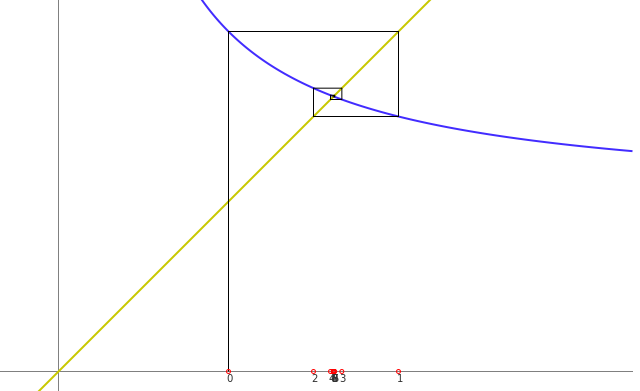
\includegraphics[width=\textwidth]{fig_fibonacci.png}
  \end{center}
  \caption{Diagramma a ragnatela relativo
    all'esercizio~\ref{ex_fibonacci}:
    sul rapporto dei termini successivi della successione di Fibonacci.\\\\
    \usebox{\qrexfibonacci}%
    }
  \label{fig_fibonacci}
\end{figure}

Un metodo grafico per visualizzare l'andamento dei termini della
successione definita da \eqref{eq1} è il \emph{diagramma a
  ragnatela}. Si disegna la curva $y=f(x)$ su un piano
cartesiano. Partendo dal punto di coordinate $(\alpha, 0)=(a_0, 0)$ si procede
lungo una retta verticale fino a raggiungere il grafico della funzione
nel punto $(a_0, f(a_0)) = (a_0, a_1)$.
Dopodiché si procede in
orizzontale fino ad incontrare la retta $y=x$ nel punto $(a_1,a_1)$ e
si ripete il procedimento in modo che le coordinate $x$ (ma anche le $y$)
dei vertici della spezzata mi danno la successione $a_0, a_1, a_2,
\dots$. Ad esempio il diagramma a ragnatela corrispondente
all'esercizio~\ref{ex_fibonacci} è rappresentato in
Figura~\ref{fig_fibonacci}.

\begin{exercise}\label{ex_3}
  Si consideri la successione definita per ricorrenza
  \[
  \begin{cases}
    a_0 = 0\\
    a_{n+1} = 1 + a_n^2.
  \end{cases}
  \]
  Determinare il limite della successione.
\end{exercise}
\newsavebox{\qrextre}\sbox{\qrextre}{%
\myqrshortdoclink{ex3}{Diagramma a ragnatela relativo all'esercizio \getrefnumber{ex_3}}}
\begin{figure}
  \begin{center}
    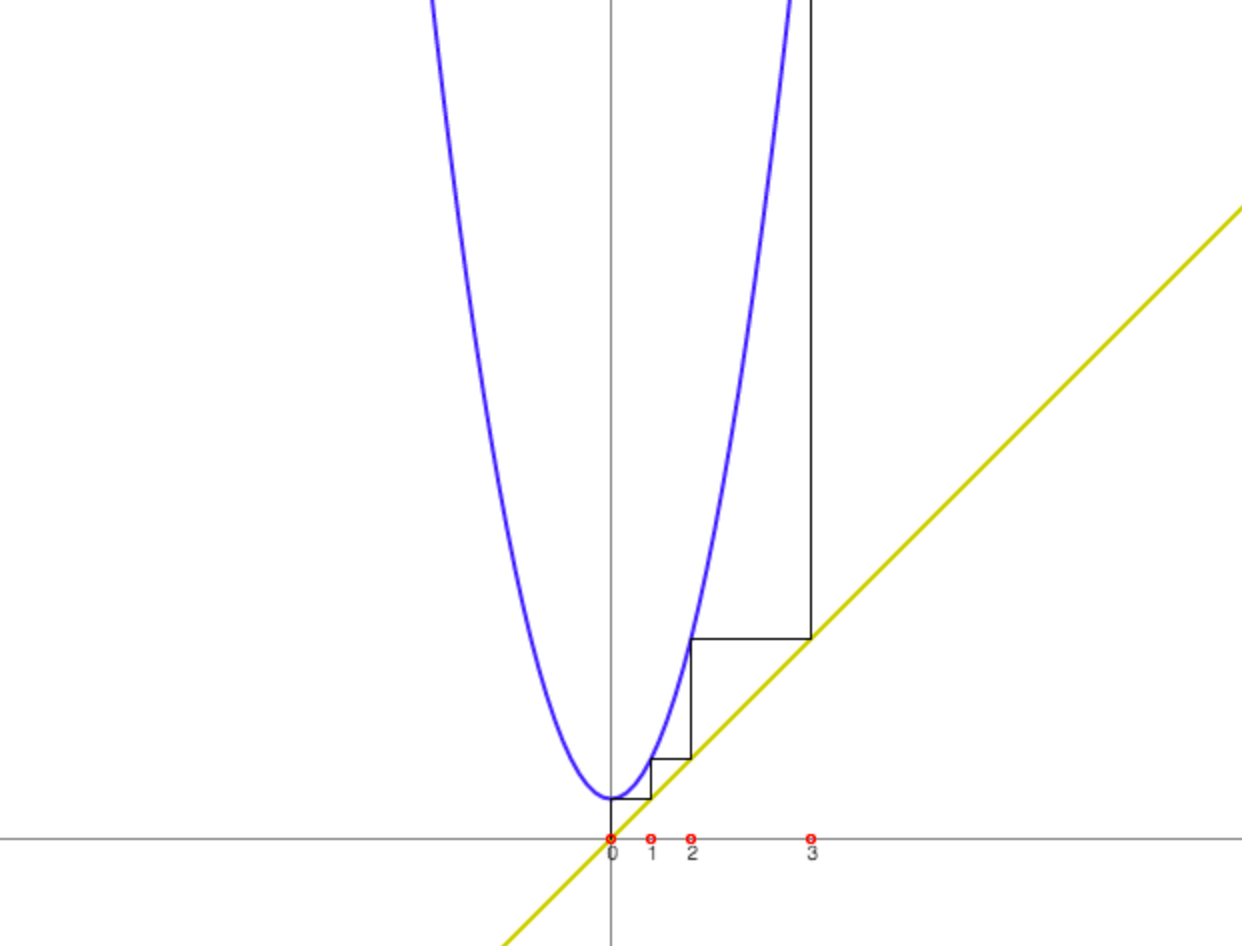
\includegraphics[width=\textwidth]{fig_ex_3.png}
  \end{center}
  \caption{Diagramma a ragnatela relativo
    all'esercizio~\ref{ex_3}.
    \ifwidemargin\\\\\fi%
    \usebox{\qrextre}}
  \label{fig_ex_3}
\end{figure}

\begin{proof}[Soluzione]
  L'equazione ricorsiva è $a_{n+1}=f(a_n)$ se poniamo $f(x) = 1+x^2$.
  E' facile verificare che per ogni $x$ si ha $f(x) > x$ e quindi, per
  il Teorema~\ref{th_1} otteniamo che la successione $a_n$ è
  crescente. Dunque ammette limite: $a_n \to \ell$. Se il limite fosse
  finito si avrebbe
  \[
  a_{n+1} = 1 + a_n^2 \to 1 + \ell^2
  \]
  e quindi, visto che $a_{n+1}\to \ell$, si avrebbe $\ell = 1 +
  \ell^2$ (cioè $\ell$ dovrebbe essere un punto fisso di $f$). Questa
  equazione abbiamo già osservato che non ha soluzioni ($x^2 + 1 > x$)
  e quindi $\ell$ non è finito. Visto che la successione $a_n$ è
  crescente possiamo escludere che sia $\ell=-\infty$ e quindi l'unica
  possibilità che rimane è che $a_n \to +\infty$.
\end{proof}

\newsavebox{\qrexquattro}\sbox{\qrexquattro}{%
\myqrshortdoclink{ex4}{Diagramma a ragnatela relativo all'esercizio \getrefnumber{ex_4}}}
\begin{figure}
  \begin{center}
  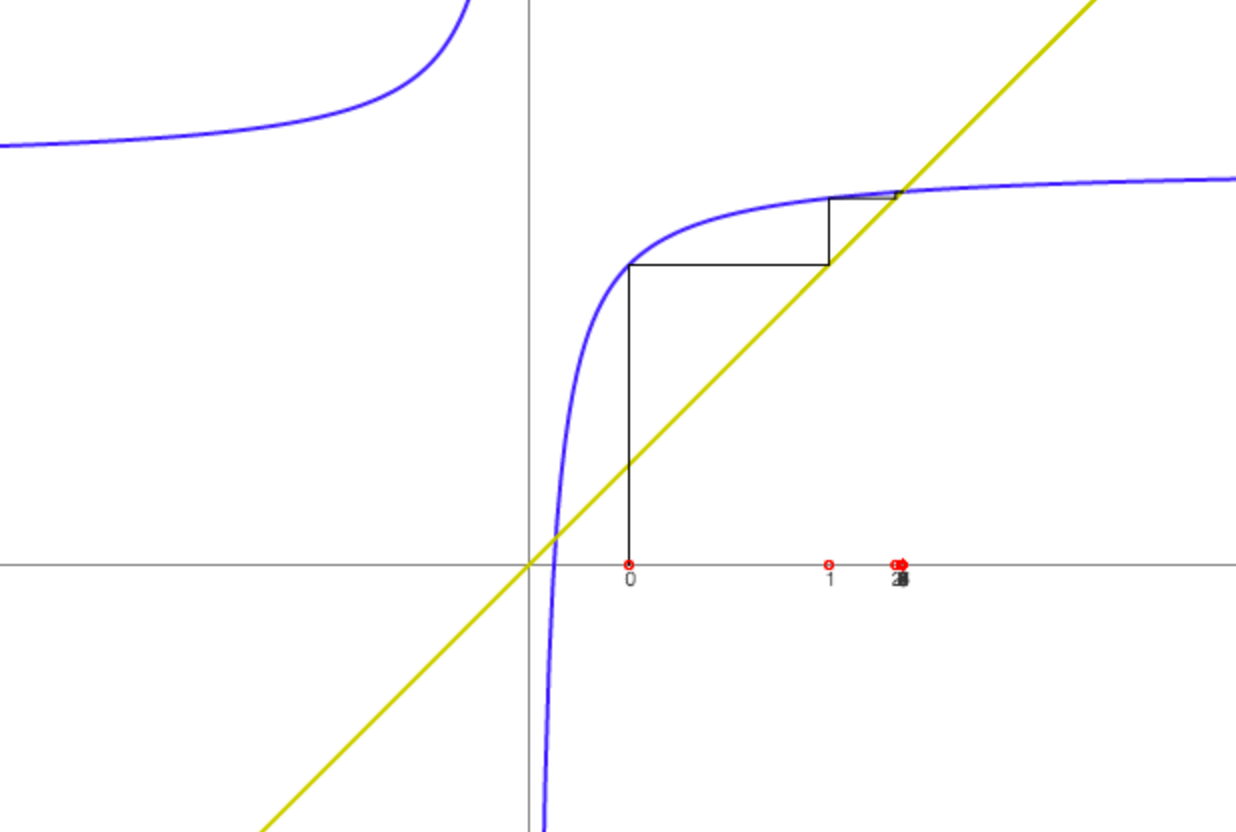
\includegraphics[width=\textwidth]{fig_ex_4.png}
  \end{center}
  \caption{Diagramma a ragnatela relativo
    all'esercizio~\ref{ex_4}.
    \ifwidemargin\\\\\fi%
    \usebox{\qrexquattro}
    }
  \label{fig_ex_4}
\end{figure}

\begin{exercise}\label{ex_4}
  Si consideri la successione definita per ricorrenza
  \[
  \begin{cases}
    a_0 = 1\\
    a_{n+1} =4-\frac 1 {a_n}.
  \end{cases}
  \]
  Determinare il limite della successione.
\end{exercise}

\begin{proof}[Soluzione]
  Si mostra che sull'intervallo $A=(2-\sqrt 3, 2+\sqrt 3)$
  vale $f(x)>x$, che gli estremi di $A$ sono punti fissi
  e inoltre che la funzione $f$ è crescente (lo è su tutto $(0,+\infty)$).
  Di conseguenza è facile verificare che $A$ è invariante, in quanto si ha
  \begin{align*}
  2-\sqrt 3 < x < 2+\sqrt 3 &\Rightarrow
  f(2-\sqrt 3) < f(x) < f(2+\sqrt 3)\\
  &\Rightarrow
  2-\sqrt 3 < f(x) < 2+\sqrt 3.
  \end{align*}

  Inoltre se $a_0 \in A$ allora per ogni $n\in\NN$ si ha $a_n\in A$ ed essendo
  $f(x)>x$ la successione sarà crescente. Dunque ammette
  limite: $a_n \to \ell \in [2-\sqrt 3,2+\sqrt 3]$, $\ell \ge a_0$.
  Ma allora
  \[
  a_{n+1} = 4-\frac 1 {a_n} \to 4 - \frac 1 \ell = f(\ell)
  \]
  e visto che $a_{n+1}$ ha lo stesso limite di $a_n$ si ha $\ell =
  f(\ell)$ le cui uniche soluzioni sono $2\pm \sqrt 3$. Ma $2-\sqrt 3$
  va scartata in quanto $\ell\ge a_0 > 2-\sqrt 3$ e quindi rimane
  $a_n \to \ell = 2+\sqrt 3$.
\end{proof}

\newsavebox{\qrexcinque}\sbox{\qrexcinque}{%
\myqrshortdoclink{ex5}{Diagramma a ragnatela relativo all'esercizio \getrefnumber{ex_5}}}
\begin{figure}
 \begin{center}
    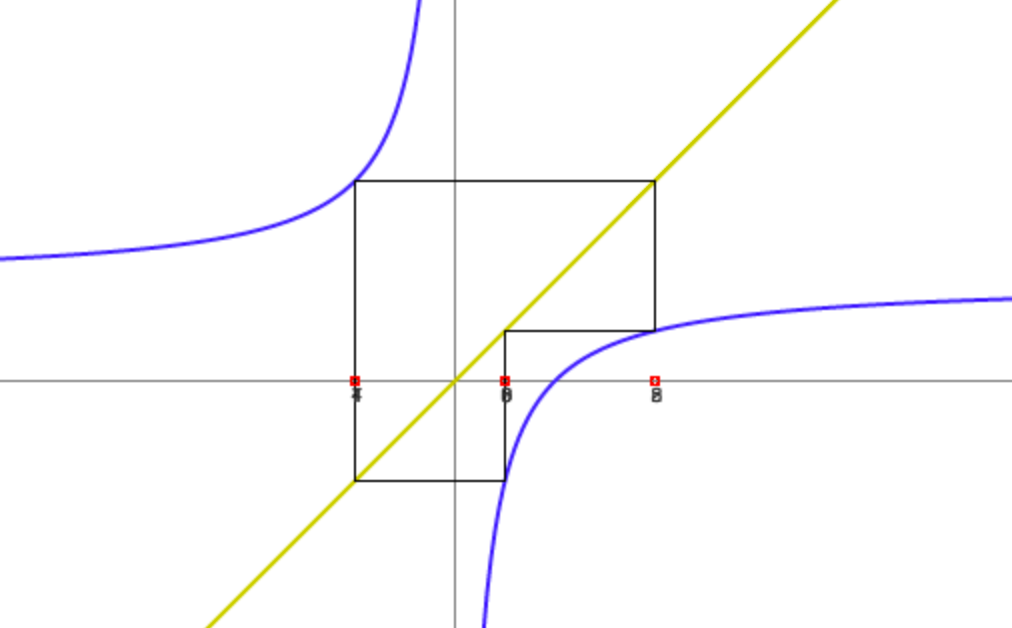
\includegraphics[width=\textwidth]{fig_ex_5.png}
  \end{center}
  \caption{Diagramma a ragnatela relativo
    all'esercizio~\ref{ex_5}.
    \ifwidemargin\\\\\fi%
    \usebox{\qrexcinque}}
  \label{fig_ex_5}
\end{figure}

\begin{exercise}\label{ex_5}
  Si consideri la successione definita per ricorrenza
  \[
  \begin{cases}
    a_0 = \frac 1 2\\
    a_{n+1} = 1 - \frac{1}{a_n}
  \end{cases}
  \]
  Determinare, se esiste, il limite della successione.
\end{exercise}

\begin{proof}[Soluzione]
  Osserviamo che:
  \begin{align*}
    a_0 &= \frac 1 2 \\
    a_1 &= 1 - \frac{1}{1/2} = -1\\
    a_2 &= 1 - \frac{1}{-1} = 2\\
    a_3 &= 1 - \frac{1}{2} = \frac 1 2 = a_0
  \end{align*}
  Essendo $a_3 = a_0$ la successione si ripete e, (per induzione) si
  dimostra che $a_{3n+k} = a_k$. Dunque si ha
  \begin{align*}
    a_{3n} &= a_0 = \frac 1 2\\
    a_{3n+1} &= a_1 = -1\\
    a_{3n+2} &= a_2 = 2
  \end{align*}
  e la successione $a_n$ non ammette limite.
\end{proof}

\newsavebox{\qrexsei}\sbox{\qrexsei}{%
\myqrshortdoclink{ex6}{Diagramma a ragnatela relativo all'esercizio \getrefnumber{ex_6}}}
\begin{figure}
  \begin{center}
    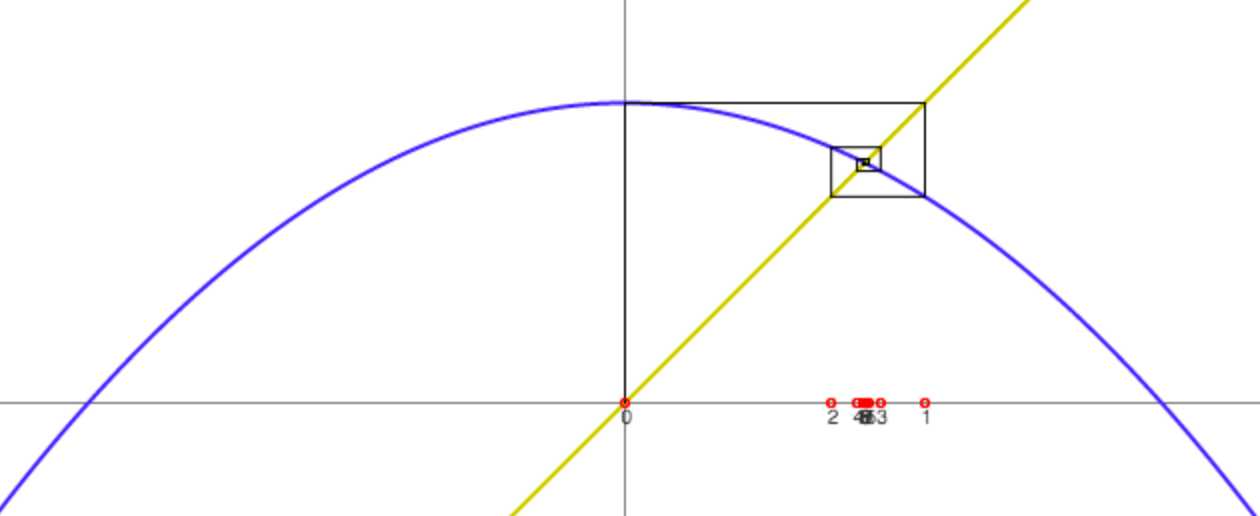
\includegraphics[width=\textwidth]{fig_ex_6.png}
  \end{center}
  \caption{Diagramma a ragnatela relativo
    all'esercizio~\ref{ex_6}.
    \ifwidemargin\\\\\fi%
    \usebox{\qrexsei}}
  \label{fig_ex_6}
\end{figure}

\begin{exercise}\label{ex_6}
  Si consideri la successione definita per ricorrenza
  \[
  \begin{cases}
    a_0 = 0\\
    a_{n+1} = \frac{5-a_n^2}{4}.
  \end{cases}
  \]
  Determinare il limite della successione.
\end{exercise}

\begin{proof}[Soluzione]
Si ha $a_{n+1} = f(a_n)$ se scegliamo $f(x) = (5-x^2)/4$. Osserviamo
che la funzione $f$ è decrescente per $x \ge 0$ (infatti $0 \le x_1 <
x_2$ implica $x_1^2 < x_2^2$ da cui $-x_1^2 > -x_2^2$ e quindi $f(x_1)
> f(x_2)$). Osserviamo inoltre che
\begin{align*}
a_0 &= 0\\
a_1 &= f(a_1) = \frac 5 4.\\
a_2 &= f\enclose{\frac 5 4} = \frac{5-25/16}{4} = \frac{55}{64}
\end{align*}
Vogliamo dimostrare che l'intervallo $A=[0,5/4]$ è invariante. Visto
che $f$ è decrescente su tale intervallo, si ha:
\begin{align*}
0 \le x \le \frac 5 4 &\Rightarrow f(0) \ge f(x) \ge f(5/4)\\
&\Rightarrow \frac 5 4 \ge f(x) \ge \frac{55}{64} \ge 0\\
&\Rightarrow 0 \le f(x) \le \frac 5 4
\end{align*}
cioè $x\in A \Rightarrow f(x)\in A$, che è quanto volevamo dimostrare.

Per il Teorema~\ref{th_decr} sappiamo dunque che $a_{2n} \to \ell$ e
$a_{2n+1} \to \ell'$. Entrambi i limiti sono finiti in quanto essendo
$a_n \in A$ per ogni $n$, si ha $\ell, \ell' \in \bar A = A$.
Dunque, come al solito, osserviamo che si ha:
\begin{align*}
  a_{2n+1} &= f(a_n) \to f(\ell)  \\
  a_{2n+2} &= f(a_{n+1}) \to f(\ell')
\end{align*}
ma sapendo che $a_{2n+1}\to \ell'$ e $a_{2n+2}\to \ell$ otteniamo il
seguente sistema:
\[
\begin{cases}
  \ell' = f(\ell)\\
  \ell = f(\ell')
\end{cases}
\]
da cui si ottiene $f(f(\ell))=\ell$ e $f(f(\ell'))=\ell'$. Dunque
vogliamo scrivere e risolvere l'equazione $f(f(x))=x$:
\[
\frac{5-\left(\frac{5-x^2}{4}\right)^2}{4} = x
\]
cioè
\[
5 - \frac{25 - 10x^2 + x^4}{16} = 4x
\]
ovvero
\[
x^4 - 10 x^2 + 64 x - 55 = 0.
\]

Come facciamo a risolvere una equazione di quarto grado?
In questo frangente dobbiamo fare una osservazione di carattere
generale che ci sarà di grande aiuto.
Osserviamo che se $x$ è una soluzione di $f(x)=x$ allora $x$
è anche soluzione di $f(f(x)) = x$ in quanto in tal caso si ha
$f(f(x))=f(x)=x$.
Ma l'equazione $f(x) = x$ è una equazione di secondo grado, che quindi
possiamo facilmente risolvere:
\begin{gather*}
  \frac{5-x^2}{4} = x \\
  x^2 + 4x - 5 = 0 \\
  x_{12} = -2 \pm \sqrt{4 + 5} = -2 \pm 3.
\end{gather*}

Dunque abbiamo trovato due zeri del polinomio di quarto grado e
tale polinomio deve essere quindi divisibile per
\[
 x^2 + 4x - 5 = (x-1)(x+5).
\]
Eseguiamo la divisione tra polinomi:
\begin{align*}
\frac{x^4 - 10 x^2 + 64 x - 55}{x^2 + 4x - 5}
&= x^2 + \frac{x^4 - 10 x^2 + 64x - 55 - x^2 (x^2 + 4x - 5)}{x^2+4x-5}\\
&= x^2 + \frac{-4x^3 - 5 x^2 + 64 x - 55}{x^2+4x-5}\\
&= x^2 - 4x + \frac{-4x^3 - 5x^2 - 64 x - 55 + 4x(x^2+4x-5)}{x^2+4x-5}
\\
&= x^2 - 4x + \frac{11 x^2 + 44 x - 55}{x^2 + 4x -5}\\
&= x^2 - 4x + 11.
\end{align*}
Come previsto la divisione non ha resto. Possiamo quindi completare la
scomposizione cercando gli zeri del polinomio $x^2-4x+11$ che però, da
un rapido controllo, non ha soluzioni reali.

Dunque in questo caso i punti fissi di $f$ coincidono con i punti
fissi di $f\circ f$ e dunque i due limiti $\ell, \ell'$ devono essere
elementi dell'insieme dei punti fissi: $\ENCLOSE{1, -5}$. D'altra parte $-5$
deve essere escluso in quanto i limiti stanno entrambi nella chiusura
dell'insieme invariante, che non comprende numeri negativi.

Concludiamo quindi che $\ell = \ell' = 1$ e dunque l'intera
successione ha limite: $a_n \to 1$.
\end{proof}

\begin{exercise}\label{ex_7}
  %% a_n <- (a_n + 2)/4
  Si consideri la successione definita per ricorrenza
  \[
  \begin{cases}
    a_0 = \alpha\\
    a_{n+1} = 4 a_n (1-a_n) % 2- a_n^2.
  \end{cases}
  \]
  Determinare il limite della successione nei casi: 
  $\alpha=-1$, 
  $\alpha=2$ e 
  $\alpha=1/42$.
\end{exercise}


\newsavebox{\qrexsette}\sbox{\qrexsette}{%
\myqrshortdoclink{ex7b}{Diagramma a ragnatela relativo all'esercizio \getrefnumber{ex_7}}}
\begin{figure}
   \begin{center}
    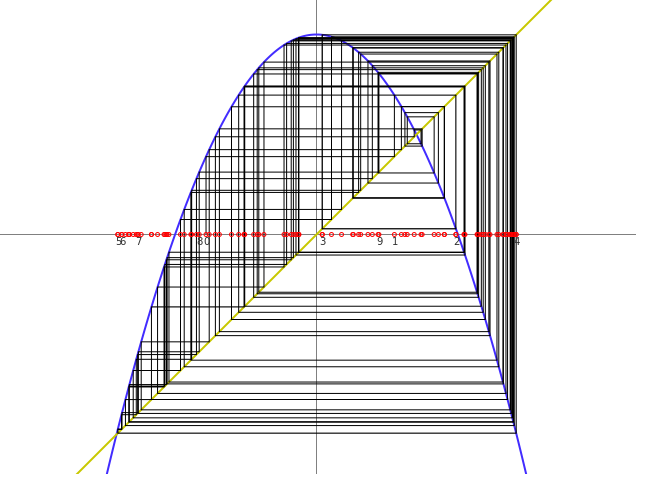
\includegraphics[width=0.5\textwidth]{fig_ex_7.png}
  \end{center}
  \caption{Diagramma a ragnatela relativo
    all'esercizio~\ref{ex_7}.
    \ifwidemargin\\\\\fi%
    \usebox{\qrexsette}}
  \label{fig_ex_7}
\end{figure}

\begin{proof}[Soluzione]
  Abbiamo $a_{n+1} = f(a_n)$ con $f(x) = 4x(1-x)$. 
  Determiniamo i punti
  fissi di $f$:
  \[
  4x(1-x)= x, \qquad 4 x^2 - 3x = 0
  \]
  che ha come soluzioni $x_1=0$ e $x_2=\frac 3 4$. 
  Tenendo conto anche dei segni si può
  osservare che all'interno delle due soluzioni si ha $f(x)>x$ mentre
  all'esterno si ha $f(x)<x$.

  Osserviamo inoltre che $f(x)$ è crescente per
  $x\le \frac 1 2$ e decrescente per $x\ge \frac 1 2$.

  Caso $\alpha=-1$. In questo caso consideriamo l'intervallo
  $A=(-\infty, 0)$. Visto che $f$ è crescente su questo intervallo,
  e visto che $0$ è un punto fisso si ha:
  \[
  x < 0 \Rightarrow f(x) < f(0) \Rightarrow f(x) < 0
  \]
  che significa che $A$ è un intervallo invariante.

  Su questo intervallo si ha $f(x)<x$ e quindi $a_n$ è decrescente e
  di conseguenza ammette limite $a_n\to \ell$. Il limite può essere
  finito oppure $-\infty$. Ma se fosse finito allora avremmo
  \[
  a_{n+1} = 4 a_n (1-a_n) \to 4 \ell (1-\ell)
  \]
  e siccome $a_{n+1}\to \ell$ avremmo che $\ell$
  è un punto fisso di $f$. 
  Ma visto che $\ell \le a_0 = \alpha < 0$
  otteniamo un assurdo.

  Dunque l'unica possibilità è che $a_n \to -\infty$. Questo
  stesso ragionamento vale per ogni $\alpha<0$.

  Caso $\alpha=2$. In questo caso si ha:
  \begin{align*}
    a_0 &= \alpha = 2\\
    a_1 &= f(a_0) = 4\cdot 2\cdot (1-2) = -8.
  \end{align*}
  quindi $a_1 \in A$ (l'intervallo invariante del punto precedente) e
  dall'indice $2$ in poi ci si riconduce quindi ai risultati
  precedenti. Dunque anche in questo caso $a_n \to -\infty$.

  Caso $\alpha = \frac 1{42}$. Questo caso è decisamente più complesso dei
  precedenti. Prendiamo l'insieme $A_2 = [0, 1]$: vogliamo dimostrare
  che è un insieme invariante. Nell'intervallo $\closeinterval{0}{\frac 1 2}$ la funzione è
  crescente e quindi ha minimo in $0$ dove vale $f(0)=0$ ed ha
  massimo in $\frac 1 2$ dove assume il valore $f(1/2) = 1$. Nell'intervallo
  $\closeinterval{\frac 1 2}{1}$ la funzione è decrescente e, di nuovo, ha massimo $f(1/2)=1$ e
  minimo $f(1)=0$. Dunque per ogni $x\in [0,1]$ si ha $f(x) \in
  [0,1]$ cioè, come volevamo dimostrare, $A_2$ è invariante.

  Dunque visto che $a_0 = \alpha \in A_2$ scopriamo che per ogni $n$
  si ha $a_n \in [0,1]$. Supponiamo ora che la successione abbia
  limite: $a_n \to \ell$. In tal caso, passando al limite
  nell'equazione $a_{n+1} = f(a_n)$ otteniamo, come al solito, che il
  limite dovrebbe essere un punto fisso di $f$: o $\ell=0$ oppure
  $\ell=\frac 3 4$. Cercheremo ora di dimostrare che questo è assurdo. Ci sono
  due possibilità che dobbiamo escludere. La prima è che la
  successione tenda al punto fisso $\ell$ senza mai uguagliarlo. La
  seconda è che per un certo $n_0$ si abbia $a_n = \ell$ per $n=n_0$ e
  quindi per ogni $n\ge n_0$.

  Supponiamo di essere nel primo caso e supponiamo che $\ell = 0$. In
  tal caso, per il teorema della permanenza del segno la successione
  deve, da un certo indice in poi, stare nell'intervallo $\closeinterval{0}{\frac 1 2}$. Ma
  in tale intervallo si ha $f(x)>x$ e quindi la successione sarebbe,
  da un certo indice in poi, crescente. Ma visto che $a_n \ge 0$ per
  ogni $n$, non è possibile che la successione converga, crescendo, a
  $0$.

  Supponiamo allora di essere nel primo caso (la successione è sempre
  diversa dai due punti fissi) e supponiamo che $\ell = \frac 3 4$. In
  questo caso da un certo indice in poi la successione deve stare
  nell'intervallo $\closeinterval{\frac 1 2}{1}$ (altrimenti non potrebbe convergere a
  $\frac 3 4$). In tale intervallo la funzione $f$ è decrescente e quindi
  le sottosuccessioni dei termini pari e dei termini dispari sono
  entrambe monotòne. Si potrebbe cercare di studiare le successioni dei
  termini pari $a_{2n}$ e dispari $a_{2n+1}$ che soddisfano una relazione di ricorrenza
  con la funzione $f\circ f$ al posto di $f$ e osservare che la successione
  che si trova a sinistra del punto fisso dovrebbe decrescere e quella che si trova a
  destra dovrebbe crescere (e questo sarebbe assurdo). Un metodo forse più
  rapido che non richiede lo studio della funzione composta è invece il seguente.
  L'idea è di osservare che $f$ tende ad aumentare le distanze quando ci si trova
  nei paraggi del punto $1$. Se per assurdo $a_n\to \frac 3 4$ allora definitivamente
  si dovrà avere $\abs{a_n-\frac 3 4}< 1/8$. Ma allora si osserva che:
  \[
    \abs{a_{n+1}-\frac 3 4}
    = \abs{4a_n(1-a_n)-\frac 3 4}
    = \abs{\frac 3 4 - 4a_n + 4a_n^2}
    = \abs{a_n-\frac 3 4}\abs{4a_n -1}
    \ge 4\abs{a_n-\frac 3 4}
  \]
  in quanto se $\abs{a_n-\frac 3 4}<1/8$ allora (per la disuguaglianza triangolare inversa)
  $\abs{4a_n-1}\ge 4$. Questo è assurdo perché significa che $\abs{a_n -\frac 3 4}\to +\infty$
  (per il criterio del rapporto) quando invece dovrebbe essere $\abs{a_n-\frac 3 4}\to 0$.

  \textbf{Nota.} Vedremo nei prossimi teoremi che
  se la derivata di $f$ è in valore assoluto minore di
  $1$ allora il punto fisso sarà stabile (o attrattivo) cioè partendo
  da un punto sufficientemente vicino si convergerà necessariamente al
  punto fisso. Se invece la derivata è in valore assoluto maggiore di
  $1$ il punto fisso sarà instabile (o repulsivo). Cioè, a parte la
  successione costante che assume il valore esatto del punto fisso,
  non è
  possibile che una successione converga al punto fisso.

  Rimane da considerare la possibilità che la successione assuma da un
  certo punto in poi il valore esatto di un punto fisso. Supponiamo ad
  esempio che per un certo $n$ si abbia $a_n=\frac 3 4$. Allora si deve avere
  \[
  \frac 3 4 = a_n = 4\cdot a_{n-1} \cdot (1-a_{n-1})
  \]
  da cui si ricava (tramite~\eqref{eq:secondo_grado})
  \[
  a_{n-1} = \frac 3 4 
  \qquad\lor\qquad
  a_{n-1} = \frac 1 4.
  \]
  Se $a_n$ era il primo termine con valore $\frac 3 4$ dovrà necessariamente
  essere $a_{n-1} = \frac 1 4$. Ma allora
  \[
  \frac 1 4 = a_{n-1} = 4 a_{n-2}(1-a_{n-2})
  \]
  da cui $a_{n-2} = \frac{2\pm\sqrt 3}{4}$. Ma ora osserviamo che essendo $a_0=
  \alpha = \frac 1 {42}$ un numero razionale, e osservando che $\QQ$ è un
  insieme invariante per $f$ (perché? verificare per induzione...)
  deduciamo che ogni $a_k \in \QQ$ e quindi
  avremmo $a_{n-2} = \frac{2\pm\sqrt 3}{4} \in \QQ$: assurdo.

  Stesso discorso si può fare se si avesse $a_n=0$, in quanto si
  avrebbe $a_{n-1} = 1$, $a_{n-2} = \frac 1 2$ e quindi $a_{n-3}=\frac{2 \pm \sqrt 2}{4}$.

  Dunque la successione $a_n$ non ammette limite.
\end{proof}

\begin{exercise}\label{ex_8}
  Si consideri la successione definita per ricorrenza
  \[
  \begin{cases}
    a_0 = \alpha\\
    a_{n+1} = \frac{1}{2-a_n}.
  \end{cases}
  \]
  Trovare il limite della successione nel caso $\alpha =
  -\the\year$. Determinare l'insieme dei valori di $\alpha$ per i quali la
  successione $a_n$ non è ben definita (in quanto per un qualche $n$ il
  denominatore $2-a_n$ si annulla).
  Trovare il limite nel caso $\alpha=\frac{\the\year}{1000}$.
\end{exercise}

\newsavebox{\qrexotto}\sbox{\qrexotto}{%
\myqrshortdoclink{ex8}{Diagramma a ragnatela relativo all'esercizio \getrefnumber{ex_8}}}
\begin{figure}
 \begin{center}
    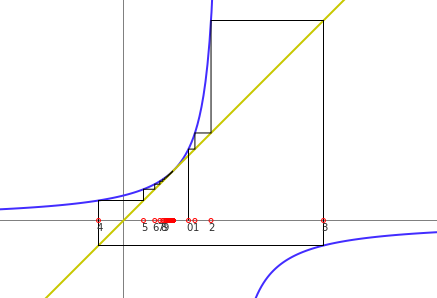
\includegraphics[width=\textwidth]{fig_ex_8.png}
  \end{center}
  \caption{Diagramma a ragnatela relativo
    all'esercizio~\ref{ex_8}.
    \ifwidemargin\\\\\fi%
    \usebox{\qrexotto}}
  \label{fig_ex_8}
\end{figure}

\begin{proof}[Soluzione]
Posto $f(x) = 1/(2-x)$
si osserva che la disequazione $f(x)\ge x$ è verificata per ogni
$x<2$. L'equazione di punto fisso $f(x)=x$ ha come unica soluzione
$x=1$. Sull'intervallo $A=(-\infty,1)$ la funzione $f$ è crescente e
l'intervallo risulta essere invariante. Dunque per
$\alpha=-\the\year \in A$ la successione risulta essere crescente e superiormente
limitata. Dunque converge $a_n\to \ell$. Passando al limite in
$a_{n+1} = f(a_n)$ si trova che $\ell$ deve essere un punto fisso di
$f$ e quindi $\ell = 1$.

La successione non è ben definita se per qualche $n$ si trovasse
$a_n=2$ in quanto la funzione $f$ non è definita per $x=2$. Altri
valori si ottengono risalendo all'indietro la successione $a_n$.
Dalla equazione
\[
a_n = \frac{1}{2-a_{n-1}}
\]
si ricava
\[
a_{n-1} = 2-\frac{1}{a_n}.
\]
L'insieme dei punti partendo da quali si arriva prima o poi in $x=2$ è
dato dunque dai valori della successione
\[
\begin{cases}
  b_1 = 2\\
  b_{n+1} = 2 - \frac{1}{b_n}.
\end{cases}
\]
Osserviamo che in questo caso specifico è possibile ricavare una
formula esplicita per il termine $b_n$. Osserviamo infatti che:
\[
b_0 = 2,\quad
b_1 = \frac{3}{2},\quad
b_2 = \frac{4}{3}
\]
e proviamo a congetturare che sia $b_n = \frac{n+1} n$. In effetti questo
si può dimostrare per induzione. Per $n=1$ si ha $(n+1)/n = 2 =
b_1$. E se supponiamo che valga $b_n = (n+1)/n$ si ha
\[
b_{n+1} = 2 - \frac{n}{n+1} = \frac{2n+2-n}{n+1} = \frac{n+2}{n+1}.
\]
Dunque l'insieme dei punti partendo dai quali la successione $a_n$ non
è ben definita è dato da:
\[
  X= \ENCLOSE{\frac{n+1}{n}\colon n \in \NN}.
\]

Per il caso $\alpha=\frac{\the\year}{1000}$ osserviamo che sull'intervallo
$A_2 = (1,2)$ si ha sempre $f(x)>x$ (ma si potrebbe osservare che
$A_2$ non è invariante). Finché $a_n$ rimane in
tale intervallo la successione risulta quindi crescente. Però non è
possibile che la successione rimanga sempre in $A_2$ perché in tal
caso il limite dovrebbe essere un punto
fisso. Ma l'unico punto fisso è $1$ che è minore di $\alpha$ e quindi
la successione, crescente, non può convergere. Necessariamente la
successione esce dall'intervallo $A_2$ (in effetti notiamo che $\alpha
\not \in X$) e, per un certo $n$ si avrà $a_n>2$. Osserviamo ora che
sull'intervallo $A_3 = (2,+\infty)$ si ha $f(x)<0$ e dunque
se $a_n\in A_2$ necessariamente $a_{n+1} \in A$. Dunque questo caso si
riconduce al primo studiato, e la successione tende a $1$.
\end{proof}

\begin{exercise}
  Si consideri la successione definita per ricorrenza
  \[
  \begin{cases}
    a_0 = \alpha\\
    a_{n+1} = \frac{a_n^2-a_n}{2}.
  \end{cases}
  \]
  Determinare al variare di $\alpha$ il limite della successione.
\end{exercise}

\begin{exercise}
  Si consideri la successione definita per ricorrenza
  \[
  \begin{cases}
    a_0 = \alpha \\
    a_{n+1} = 1 - a_n^2.
  \end{cases}
  \]
  Determinare al variare di $\alpha$ il limite della successione.
\end{exercise}

\begin{exercise}
  Calcolare il limite della successione $a_n$ 
  definita per ricorrenza da:
    \[
    \begin{cases}
      a_0 = 1\\
      a_{n+1} = 1 - \frac {4}{a_n^2}.
    \end{cases}
    \]
  \end{exercise}
  
\begin{exercise}
  Calcolare il limite della successione $a_n$
  definita per ricorrenza da:
  \[
    \begin{cases}
      a_0 = 10\\
      a_{n+1} = a_n \cdot (\abs{a_n}-1).
    \end{cases}
  \]
\end{exercise}
  
\begin{exercise}
Calcolare
\[
 1 + \frac{1}{1+\frac{1}{1+\frac{1}{1+\frac{1}{\dots}}}}
\]
\end{exercise}

\begin{exercise}
Calcolare
\[
  \lim_{x\to 1^+} \sqrt{x-\sqrt{x- \sqrt{x-\sqrt{x - \dots}}}}
\]
\end{exercise}

\begin{exercise}[Mandelbrot reale]
\label{ex:mandelbrot_reale}
Si consideri, fissato il parametro $c$, la successione definita per ricorrenza:
\[
  \begin{cases}
    a_0 = 0\\
    a_{n+1} = a_n^2 + c.
  \end{cases}
\]

Determinare i valori di $c\in \RR$ per i quali la successione $a_n$ risulta
essere limitata.
\end{exercise}
%
\begin{proof}[Svolgimento.]
\emph{Caso 1: $c > \frac 1 4$}.
In tal caso non ci sono punti fissi, in quanto l'equazione $x=x^2+c$ ha
discriminante negativo. Significa che $x^2+c > x$ per ogni $x\in \RR$. Dunque
la successione $a_n$ è strettamente crescente e tende a $+\infty$.
Non è limitata.

\emph{Caso 2:} $0\le c \le \frac 1 4$.
In questo caso l'equazione $x=x^2+c$ ha due soluzioni entrambe positive
(le soluzioni hanno somma $1$ e prodotto $c\ge 0$).
Se chiamiamo $x_1$ la più piccola delle due soluzioni possiamo dimostrare che
l'intervallo $[0,x_1)$ è invariante. Infatti su tali intervallo la funzione
$f(x)=x^2+c$ è crescente, dunque se $0\le x < x_1$ si ha $f(0) \le f(x) < f(x_1)$
cioè $c \le f(x) < x_1$. Visto che $c\ge 0$ abbiamo mostrato che l'intervallo è
invariante e la successione è dunque limitata.
Se $c=0$ la successione $a_n$ rimane costante $a_n=0$. Se $c>0$ la successione
converge al punto fisso $x_1$. In ogni caso è limitata.

\emph{Caso 3:} $-1 \le c < 0$.
In questo caso vogliamo mostrare che l'intervallo $[c,0]$ è invariante.
La funzione $f(x) = x^2+c$ è decrescente su tale intervallo, dunque
se $c\le x \le 0$ risulta $f(0)\le x \le f(c)$. Ma $f(0)=c$ e $f(c)=c^2+c
= c(c+1) \le 0$ se $c\ge -1$. Dunque $[c,0]$ è invariante e $a_n$ rimane
limitata in tale intervallo.

\emph{Caso 4:} $-2\le c < -1$.
In questo caso l'equazione $x=x^2+c$ ha una soluzione negativa ed una soluzione
positiva. Chiamiamo $x_2$ la soluzione positiva. Vogliamo mostrare che
l'intervallo $[c,x_2]$ è invariante.
La funzione $f(x)=x^2+c$ è decrescente in $[c,0]$ e crescente in $[0,x_2]$.
Se $0\le x \le x_2$ si ha dunque $f(0)\le f(x) \le f(x_2)$
cioè $c \le f(x) \le x_2$. Dunque i punti in $[0,x_2]$ rimangono nell'intervallo
$[c,x_2]$.
Se invece $c\le x \le 0$ si ha $f(0)\le f(x) \le f(c)$ cioè $c \le f(x) \le c^2+c$.
Affinché sia $c^2+c\le x_2$ basta verificare che $f(c^2+c)\le c^2+c$
cioè:
\[
  (c^2+c)^2 + c \le c^2+c
\]
che, sviluppando il quadrato, si riduce a $c^3(c+2)\le 0$ che è verificata
se $-2 \le c \le 0$.
Dunque l'intervallo $[c,x_2]$ è invariante. La successione rimane dunque
limitata in tale intervallo.

\emph{Caso 5:} $c < -2$.
In questo caso $a_0=0$, $a_1=c$, $a_2=c^2+c$ e possiamo verificare che
$c^2+c > x_2$ in quanto, come nel caso precedente, questo accade se
\[
   (c^2+c)^2 + c > c^2+c
\]
che si riduce a $c^3(c+2)>0$ che è verificata se $c<-2$.
Ma l'intervallo $(x_2,+\infty)$ è invariante e su tale intervallo
si ha $f(x)>x$ dunque la successione $a_n$ è strettamente crescente per $n\ge 2$
e diverge a $+\infty$. Non è dunque limitata.

\emph{Conclusione}. La successione è limitata se $c\in[-2,1/4]$.
Altrimenti $a_n\to +\infty$.

\end{proof}


\section{approfondimenti}

I risultati esposti finora non richiedevano
alcuna nozione del calcolo differenziale
e potevano essere compresi utilizzando solamente
le nozioni del capitolo~\ref{ch:successioni}.
In questo capitolo useremo invece
alcuni concetti che riguardano il calcolo differenziale.

\begin{theorem}[criterio per la stabilità di un punto fisso]
Sia $x_0\in \RR$, $R>0$, $I=(x_0 - R, x_0+R)$ e $f\colon I \to \RR$
una funzione che ha $x_0$ come punto fisso.
Se $f$ è $L$-lipschitziana su $I$ con $L<1$ allora $I$ è un intervallo
invariante per $f$ e se $a_n$ è una successione che soddisfa la relazione di ricorrenza $a_{n+1} = f(a_n)$ con $a_0 \in I$
allora $a_n \to x_0$ per $n\to +\infty$.

In particolare se $f\in C^1(I)$ con punto fisso $x_0 \in I$ e $\sup\ENCLOSE{\abs{f'(x)}\colon x\in I} < 1$ allora $I$ è invariante ed ogni successione $a_n$ definita per ricorrenza da $a_{n+1}=f(a_n)$ con $a_0 \in I$ converge ad $x_0$.

Ancora più in particolare, se $f$ è di classe $C^1$ in un intorno di un punto $x_0$, se $x_0$ è punto fisso di $f$ e $\abs{f'(x_0)}<1$ allora
esiste un intorno $I$ di $x_0$ che è invariante per $f$ e ogni successione $a_n$ definita per ricorrenza tramite $a_{n+1}= f(a_n)$ con $a_0\in I$ converge ad $x_0$.
\end{theorem}
  %
\begin{proof}
Osserviamo che se $f$ è di classe $C^1$ in un intorno di $x_0$ e $\abs{f'(x_0)} < 1$ allora, per continuità, esiste $L<1$ tale $\abs{f'(x)} < L$ per ogni $x$ in un intorno $I$ di $x_0$. Dunque $\sup\ENCLOSE{\abs{f'(x)}\colon x \in I} \le L < 1$ e la funzione $f$ risulta dunque essere $L$-lipschitziana. E' chiaro quindi che la seconda e la terza parte del teorema si riconducono alla prima, che è quella che andremo ora a dimostrare.

Se $f$ è $L$-lipschitziana e $x_0$ è punto fisso di $f$ osserviamo che si ha
\[
\abs{f(x) - x_0} = \abs{f(x) - f(x_0)} \le L \abs{x-x_0}
\]
da cui se $\abs{x - x_0} < R$ anche $\abs{f(x) - x_0} < R$.
Dunque $I = (x_0-R, x_0+R)$ è invariante.
Possiamo poi dimostrare per induzione che risulta
\[
 \abs{a_n - x_0} \le L^n \cdot \abs{a_0-x_0}.
\]
Infatti per $n=0$ la relazione è una uguaglianza. Il passo induttivo si ottiene osservando che
\begin{align*}
\abs{a_{n+1} - x_0}
 &= \abs{f(a_n) - f(x_0)}
 \le L \abs{a_n - x_0} \\
 &\le L\cdot L^n\abs{a_0-x_0}
 = L^{n+1}\abs{a_0-x_0}.
\end{align*}

Ma ora se $L<1$ si ha $L^n\to 0$ e dunque $\abs{a_n -x_0} \to 0$ come volevamo dimostrare.
\end{proof}

\begin{theorem}[instabilità del punto fisso]
Sia $f$ di classe $C^1$ in un intorno di un suo punto fisso $x_0$.
Se $\abs{f'(x_0)}>1$ allora non esiste una successione $a_n$ che soddisfa la relazione ricorsiva $a_{n+1} = f(a_n)$ e tale che $a_n \to x_0$ a meno che non si abbia $a_n = x_0$ da un certo indice $n$ in poi.
\end{theorem}
%
\begin{proof}
Per continuità della derivata esisterà $L>1$ e un intervallo $I$
intorno di $x_0$ tale che per ogni $x\in I$ si abbia $\abs{f'(x)} > 1$.
Se $a_n \to x_0$ allora da un certo indice $n$
in poi si avrà $a_n \in I$.
Se $a_n$ verifica la relazione ricorsiva $a_{n+1} = f(a_n)$ possiamo
allora applicare il teorema di Lagrange per ottenere che per ogni $n$ esiste $b_n$ compreso tra $x_0$ e $a_n$ tale che:
\begin{align*}
  \abs{a_{n+1} - x_0}
  &= \abs{f(a_n) - f(x_0)}
  = \abs{f'(b_n)(a_n - x_0)} \\
  &\ge L \cdot \abs{a_n - x_0} \ge \abs{a_n - x_0}.
\end{align*}
Risulta quindi che la distanza $\abs{a_n - x_0}$ deve essere crescente
e quindi l'unica possibilità perché $a_n \to x_0$ è che sia $a_n = x_0$.
\end{proof}


\section{equazioni ricorsive lineari}
\label{sec:ricorrenza_lineare}

Fissate le costanti $c_0, c_1, \dots, c_n$,
con $c_n \neq 0$,
diremo che l'equazione ricorsiva:
\begin{equation}\label{eq:ricorsione_lineare}
  c_n \cdot a_{k+n} + c_{n-1} \cdot a_{k+n-1} + \dots
    + c_1 \cdot a_{k+1} + c_0 \cdot a_k = 0
\end{equation}
è una \emph{equazione ricorsiva lineare}%
\mymargin{equazione ricorsiva lineare}\index{equazione!ricorsiva!lineare} (omogenea) di ordine $n$.
Il polinomio $P$ con gli stessi coefficienti:
\[
  P(\lambda) = c_n \cdot \lambda^n + c_{n-1}\cdot \lambda^{n-1} + \dots + c_1 \cdot \lambda + c_0
\]
si chiama \emph{polinomio caratteristico}%
\mymargin{polinomio caratteristico}\index{polinomio!caratteristico}
\index{equazione!ricorsiva!lineare!polinomio caratteristico}%
\index{polinomio!caratteristico!di una equazione ricorsiva lineare}%
associato all'equazione
lineare~\eqref{eq:ricorsione_lineare}.

Ad esempio la successione di Fibonacci $F_k$ definita da~\eqref{eq:Fibonacci}
è una soluzione dell'equazione ricorsiva lineare del secondo ordine:
\[
   a_{k+2} - a_{k+1} - a_{k} = 0
\]
il cui polinomio caratteristico è
\[
  P(\lambda) = \lambda^2 - \lambda - 1.
\]

\begin{theorem}[indipendenza delle successioni esponenziali]
\label{th:indipendenza_successioni_esponenziali}
Siano $\lambda_1, \dots, \lambda_n$ numeri complessi distinti. 
Allora le successioni $\vec a_j$ definite da
\[
  \vec a_j (k) = \lambda_j^k
\]
sono vettori indipendenti nello spazio vettoriale complesso $\CC^\NN$ di tutte le
successioni a valori complessi.
\end{theorem}
%
\begin{proof}
Dobbiamo mostrare che se una combinazione lineare delle
successioni $\vec a_j$ è nulla allora tutti i coefficienti
sono nulli. 
Lo dimostriamo per induzione sul numero $n$. 
Se $n=1$ il risultato è banale. 
Supponiamo allora di sapere che $a_1,\dots, a_{n-1}$ sono indipendenti 
e dimostriamo che allora anche $a_1,\dots, a_n$ lo sono.

Supponiamo quindi di avere $c_1, \dots, c_n\in \CC$ tali che
\[
  \sum_{j=1}^n c_j \vec a_j = \vec 0 \in \CC^\NN.
\]
Significa che per ogni $k\in \NN$ si ha
\begin{equation}\label{eq:47862}
  \sum_{j=1}^n c_j \lambda_j^k = 0.
\end{equation}
Se al posto di $k$ mettiamo $k+1$ si ha
\[
  \sum_{j=1}^n c_j \lambda_j^{k+1} = 0.
\]
Se ora moltiplichiamo \eqref{eq:47862} per $\lambda_n$ e
sottraiamo l'equazione precedente si ottiene:
\[
  \sum_{j=1}^n c_j \lambda_j^k(\lambda_n - \lambda_j) = 0.   
\]
Posto $b_j = c_j (\lambda_n - \lambda_j)$ si ottiene dunque,
per ogni $k\in \NN$
\[
 \sum_{j=1}^{n-1}  b_j \lambda_j^k = 0.
\]
Per ipotesi induttiva sappiamo che i coefficienti $b_1,\dots, b_{n-1}$ 
devono essere tutti nulli che significa, 
essendo $\lambda_n-\lambda_j\neq 0$ che anche $c_1,\dots, c_{n-1}$ 
sono tutti nulli. 
Ma allora \eqref{eq:47862} diventa 
\[
  c_n \lambda_n^k = 0  
\]
che per $k=0$ implica che anche $c_n=0$.
\end{proof}

\begin{proof}[dimostrazione alternativa]
Valutando l'equazione~\eqref{eq:47862} per $k=0,\dots, n-1$ si ottiene
\begin{align*}
  c_1 + c_2 + \dots + c_n & = 0 \\
  c_1 \lambda_1 + c_2 \lambda_2 + \dots + c_n \lambda_n & = 0 \\
  &\quad \vdots\\
  c_1 \lambda_1^{n-1} + c_2 \lambda_2^{n-1} + \dots + c_n \lambda_n^{n-1} & = 0
\end{align*}
che è un sistema lineare la cui matrice associata è
la matrice di \emph{Vandermonde}%
\mymargin{Vandermonde}\index{Vandermonde}
\index{matrice!di Vandermonde}%
\[
V =
\begin{pmatrix}
  1 & 1 &  \dots & 1 \\
  \lambda_1 & \lambda_2 & \dots & \lambda_n \\
  \lambda_1^2 & \lambda_2^2 & \dots & \lambda_n^2 \\
  \vdots & \vdots & \vdots & \vdots \\
  \lambda_1^{n-1} & \lambda_2^{n-1} & \dots & \lambda_n^{n-1}
\end{pmatrix}
\]
che notoriamente (lo si può dimostrare per induzione)
ha determinante
\[
  \det V = \prod_{j=2}^{n} \prod_{k=1}^{j-1}(\lambda_j-\lambda_k)
\]
e dunque
è invertibile se e solo se
i $\lambda_j$ sono tra loro distinti.

Dunque $c_1 = c_2 = \dots = c_n = 0$ è l'unica soluzione
del sistema lineare.
\end{proof}

\begin{theorem}[dimensione delle soluzioni]
\label{th:dimensione_ricorsione_lineare}
L'insieme $W$ di tutte le successioni soluzioni dell'equazione~\eqref{eq:ricorsione_lineare}
di ordine $n$
è un sottospazio vettoriale di dimensione $n$
dello spazio $\CC^\NN$ di tutte le successioni.
\end{theorem}
%
\begin{proof}
Denotiamo con $\vec a \in \CC^\NN$ la successione $a_k = \vec a(k)$.
L'insieme $W$ delle soluzioni dell'equazione~\eqref{eq:ricorsione_lineare}
è un sottospazio vettoriale di $\CC^\NN$ in quanto se $\vec a$
e $\vec b$ sono soluzioni anche $\vec a + \vec b$ è soluzione e se $\vec a$
è soluzione anche $t \vec a$ è soluzione per ogni $t\in \CC$
(si faccia la verifica).

Consideriamo allora l'operatore (chiamato \emph{jet}%
\mymargin{jet}\index{jet}) $J\colon W \to \CC^n$
definito da
\[
  J(\vec a) = \enclose{\vec a(0), \vec a(1), \dots, \vec a(n-1)}.
\]
E' facile verificare che $J$ è un operatore lineare in quanto la valutazione
di una funzione in un punto è una operazione lineare.

Vogliamo ora determinare
\[
  \ker J = \ENCLOSE{\vec a \in W \colon J(\vec a)=0}.
\]
Se $\vec a\in \ker J$ significa che i primi $n$ termini
della successione
$a_0, a_1, \dots, a_{n-1}$ sono tutti nulli.
Ma se $\vec a\in W$ sappiamo che vale~\eqref{eq:ricorsione_lineare} e dunque
anche $a_n$ è nullo. Applicando~\eqref{eq:ricorsione_lineare} ricorsivamente
otteniamo che $a_{n+k}=0$ per ogni $k\in \NN$ e dunque $\vec a = 0$.
Dunque $\ker J = \ENCLOSE{\vec 0}$
e per le note proprietà degli operatori lineari possiamo
affermare che $J\colon W \to \CC^n$ è iniettivo.
Dunque $\dim W \le \dim \CC^n = n$.

Ma possiamo anche osservare che $J$ è suriettivo in quanto
fissati i valori di $a_0,a_1, \dots, a_{n-1}$ l'equazione
~\eqref{eq:ricorsione_lineare} ci permette di determinare,
induttivamente, tutti i termini successivi. Dunque
fissato $\vec y = (y_0, \dots, y_{n-1}) \in \CC^n$
è possibile trovare $\vec a \in W$ tale che $J(\vec a) = \vec y$.

Visto che $J\colon W\to\CC^n$ è iniettivo e suriettivo
concludiamo che $\dim W = \dim \CC^n = n$.
\end{proof}

\begin{theorem}[caratterizzazione delle soluzioni]
Se il polinomio caratteristico dell'equazione~\eqref{eq:ricorsione_lineare}
ha $n$ zeri distinti $\lambda_1, \dots, \lambda_n$
allora
ogni soluzione dell'equazione si scrive nella forma
\[
  a_k = c_1 \lambda_1^k + c_2 \lambda_2^k + \dots + c_n \lambda_n^k
\]
dove $c_1, \dots, c_n$ sono costanti arbitrarie.
\end{theorem}
%
\begin{proof}
Sia $V=\CC^\NN$ lo spazio vettoriale di tutte le successioni.
Possiamo definire l'operatore di \emph{shift} $\sigma\colon V\to V$
\[
  (\sigma \vec a)(k) = \vec a(k+1).
\]
Risulta quindi che $a_{k+n} = (\sigma^n \vec a)(k)$ dove
$\sigma^n = \sigma \circ \sigma \circ \dots \circ \sigma$
è la composizione di $\sigma$ con se stesso per $n$ volte.
Possiamo quindi riscrivere l'equazione~\eqref{eq:ricorsione_lineare} nella forma
\[
  c_n \sigma^n \vec a + \dots + c_0 \sigma^0 \vec a = 0
\]
ovvero
\[
  P(\sigma)\vec a = 0
\]
dove con $P(\sigma)$ si intende l'operatore $P(\sigma)\colon V\to V$
ottenuto applicando il polinomio caratteristico $P$ all'operatore $\sigma$.

Se $\lambda_1,\dots,\lambda_n$ sono le $n$ radici del polinomio $P$ si può
decomporre il polinomio $P$ tramite il teorema~\ref{th:Ruffini} di Ruffini
\begin{equation}\label{eq:375628}
  P(\lambda)
  = a_n (\lambda -\lambda_1)(\lambda- \lambda_2)\cdots (\lambda - \lambda_n).
\end{equation}
la stessa decomposizione può essere fatta per $P(\sigma)$
e quindi l'equazione~\eqref{eq:ricorsione_lineare}
può essere scritta nella forma:
\begin{equation}\label{eq:437343}
(\sigma - \lambda_1 I)\circ (\sigma-\lambda_2 I)\circ \dots \circ (\sigma -\lambda_n I) \vec a = 0
\end{equation}
dove $I\colon V\to V$ è l'operatore identità $I\vec a = \vec a$.
Visto che nella decomposizione~\eqref{eq:375628}
l'ordine in cui vengono moltiplicati i fattori non conta,
anche nell'equazione~\eqref{eq:437343} possiamo applicare gli operatori
$(\sigma -\lambda_j I)$ in qualunque ordine (gli operatori commutano).
Dunque è immediato accorgersi che se $\vec a$ risolve
\[
  (\sigma - \lambda_j I) \vec a = 0
\]
per un qualunque $j=1,\dots, n$ allora $\vec a\in W$.
Ma quest'ultima equazione è facile da risolvere in quanto
ponendo $a_k = \vec a(k)$ si esplicita nella forma:
\[
  a_{k+1} - \lambda_j a_k = 0
\]
che è soddisfatta se
se si sceglie $a_k = \lambda_j^k$.

Dunque la successione $\vec a_j$ definita da
\[
  \vec a_j(k) = \lambda_j^k
\]
è un elemento di $W$.
Per $j=1,\dots, n$ abbiamo trovato $n$ soluzioni distinte
$\vec a_1, \dots, \vec a_n$. Queste soluzioni sono
indipendenti grazie al teorema~\ref{th:indipendenza_successioni_esponenziali}
e quindi essendo $\dim W = n$ per il teorema~\ref{th:dimensione_ricorsione_lineare}
possiamo affermare che queste soluzioni formano una base di $W$
che è esattamente quanto volevamo dimostrare.
\end{proof}

\begin{example}[formula esplicita per la successione di Fibonacci]
\index{successione!di Fibonacci}%
\index{Fibonacci!formula esplicita}%
La successione di Fibonacci $F_k$ definita da~\eqref{eq:Fibonacci}
soddisfa una equazione ricorsiva lineare del secondo ordine con polinomio associato
$P(\lambda) = \lambda^2 - \lambda - 1$. Risolvendo l'equazione $P(\lambda)=0$
si trovano le due radici distinte:
\[
  \lambda_{1,2} = \frac{1 \pm \sqrt{5}}{2}.
\]
La radice più grande, $\lambda_2$, corrisponde al
\emph{rapporto aureo}%
\mymargin{rapporto aureo}\index{rapporto!aureo} che usualmente viene chiamato $\phi$.
\index{$\phi$}%
Visto che $\lambda_1 \lambda_2 = -1$ si trova $\lambda_1 = -1/\phi$.
Dunque, per il teorema precedente, sappiamo che esistono due costanti $c_1$ e
$c_2$ tali che
\[
  F_k = c_1 \frac{(-1)^k}{\phi^k} + c_2 \phi^k .
\]
Imponendo le condizioni $F_0=0$, $F_1=1$ (imporre $F_2 = 1$ è equivalente a $F_0=0$)
si ottiene
\[
  c_1 + c_2 = 0, \qquad - \frac{c_1}{\phi} + c_2 \phi  = 1
\]
da cui è possibile trovare $c_1 = - c_2 = 1/\sqrt{5}$ e ottenere
così la formula di Binet per il $k$-esimo numero di Fibonacci:
\mymargin{Formula di Binet}%
\index{Fibonacci}%
\index{successione!di Fibonacci}%
\index{formula!di Binet}%
\index{Binet!formula di}%
\[
  F_k = \frac{\phi^k}{\sqrt 5} + \frac{(-1)^{k+1}}{\sqrt 5\phi^k}.
\]
Risulta piuttosto sorprendente osservare che i valori $F_k$ ottenuti
con questa espressione siano tutti numeri interi.
\end{example}



\section{dinamica complessa}
\label{sec:mandelbrot}
\index{dinamica!complessa}

Più in generale potremmo considerare successioni $z_n$ a valori complessi
e quindi equazioni ricorsive della forma
\[
  \begin{cases}
    z_0 = \alpha, \\
    z_{n+1} = f(z_n)
  \end{cases}
\]
con $f\colon \CC \to \CC$.
Se $f$ fosse lineare si potrebbe scrivere esplicitamente la soluzione
seguendo le idee presentate nella sezione~\ref{sec:ricorrenza_lineare}.

Possiamo provare a considerare la più semplice funzione non lineare che ci possa
venire in mente cioè $f(z) = z^2 + c$ e il più semplice dato iniziale $\alpha = 0$
e il problema diventa quello di studiare il comportamento delle successioni:
\begin{equation}\label{eq:mandelbrot}
  \begin{cases}
    z_0 = 0, \\
    z_{n+1} = z_n^2 + c
  \end{cases}
\end{equation}
con $c\in \CC$.

L'insieme dei numeri reali è invariante, dunque se $c\in \RR$ la successione
$z_n$ rimane reale e coincide con la successione che abbiamo
studiato nell'esercizio~\ref{ex:mandelbrot_reale}.

\begin{figure}
\begin{center}
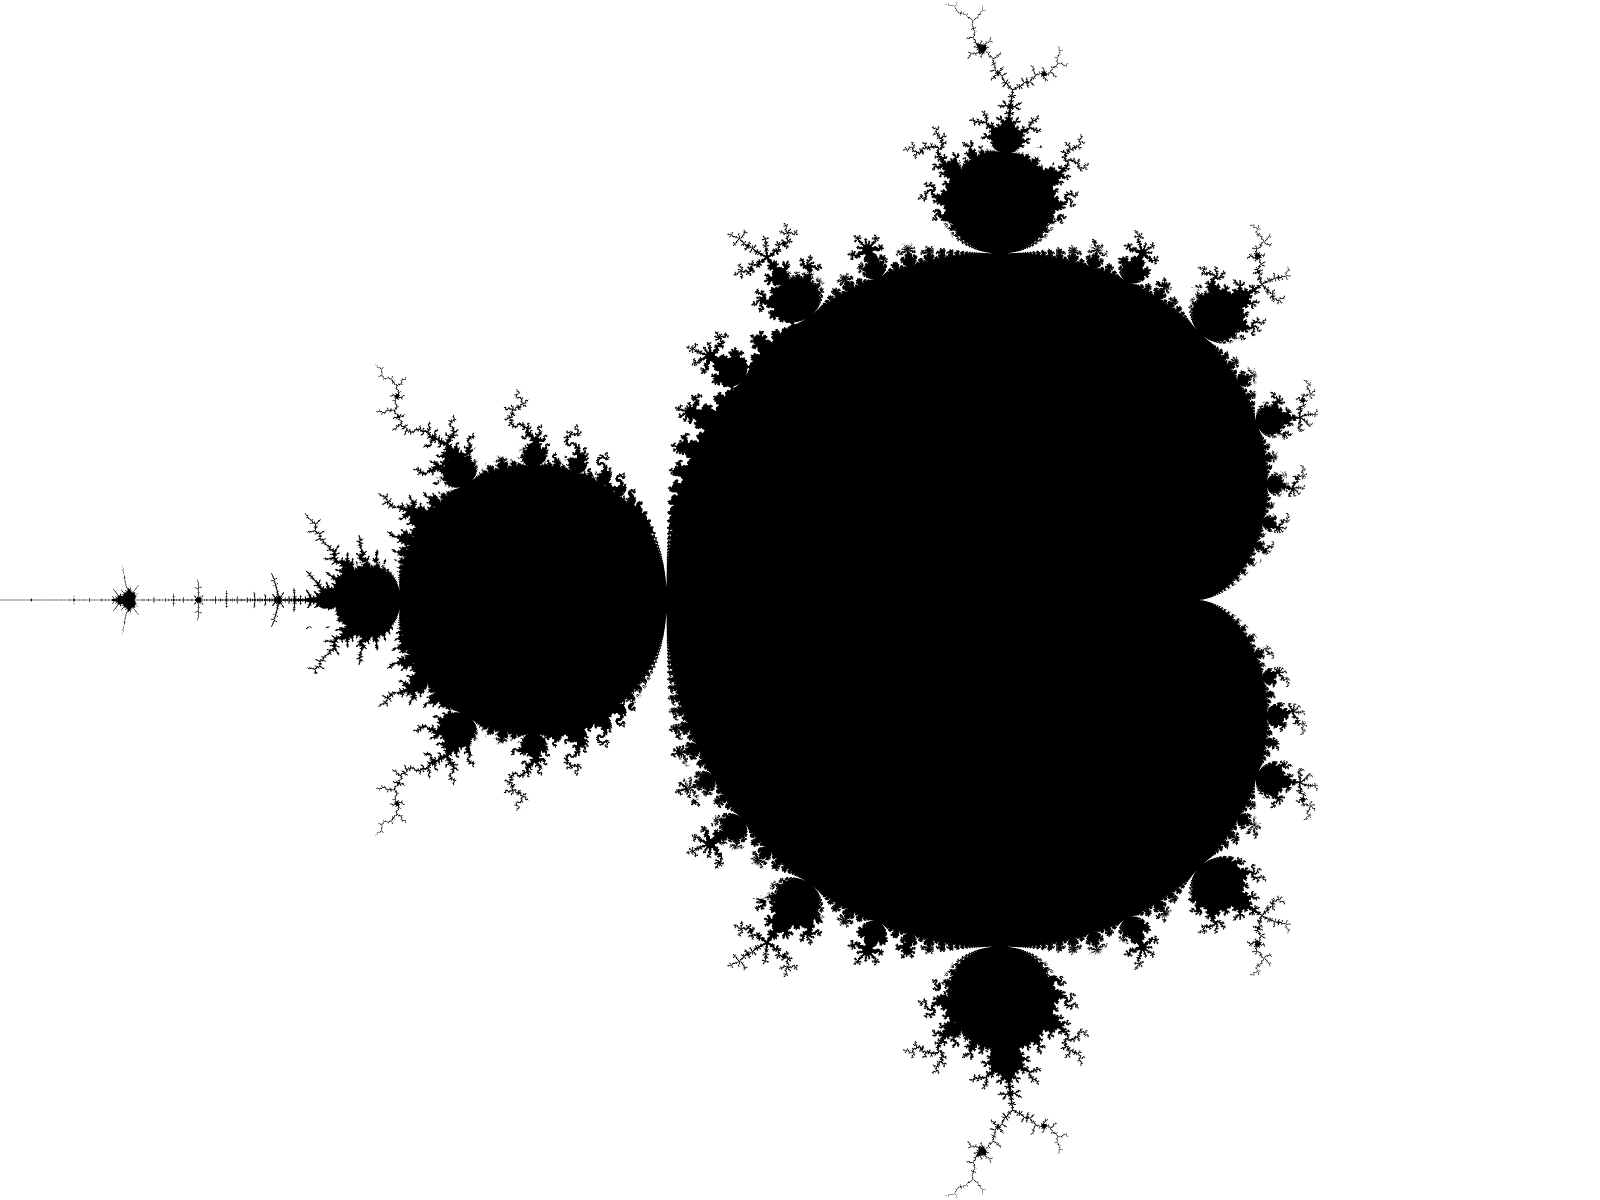
\includegraphics[width=\textwidth]{mandelbrot.png}
\end{center}
\caption{L'insieme di Mandelbrot generato al computer. Si veda il
codice a pagina \pageref{code:Mandelbrot}.}
\label{fig:mandelbrot}
\end{figure}

E' molto complicato determinare il carattere delle successioni definite
dal sistema~\eqref{eq:mandelbrot}.
Solo con l'utilizzo dei primi calcolatori
Mandelbrot (1924-2010) riuscì a rappresentare graficamente
\mymargin{insieme di Mandelbrot}%
\index{insieme!di Mandelbrot}%
\index{Mandelbrot!insieme di}%
l'insieme $M$ dei punti $c\in \CC$ per i quali la successione $z_n$ non diverge:
si veda la figura~\ref{fig:mandelbrot}.

Con l'esercizio~\ref{ex:mandelbrot_reale}
abbiamo trovato l'intersezione $M\cap \RR = [-2,1/4]$.
Nel seguente esercizio ci proponiamo ora di dimostrare un'altra semplice
proprietà che può essere
molto utile negli algoritmi numerici utilizzati per disegnare tale insieme.

\begin{exercise}[raggio di fuga]
Dimostrare che se $z_n$ è soluzione di \eqref{eq:mandelbrot}
se per un qualche $N\in \NN$ si ha $\abs{z_N}> 2$ allora $\abs{z_n}\to +\infty$
per $n\to +\infty$. In particolare l'insieme $M$ di Mandelbrot
è contenuto nel disco $\ENCLOSE{z\in \CC \colon \abs{z}\le 2}$.
\end{exercise}
%
\begin{proof}[Soluzione]
Sia $c\in \CC$ fissato e si $z_n$ la successione definita da~\eqref{eq:mandelbrot}.
Per ogni $\eps>0$ consideriamo l'insieme:
\[
  A_\eps = \ENCLOSE{z \in \CC \colon \abs{z}\ge c \text{ e } \abs{z}\ge 2+\eps}.
\]
Possiamo mostrare che l'insieme $A_\eps$ è invariante in quanto se $z_n\in A_\eps$
si ha
\begin{equation}\label{eq:473244}
\begin{aligned}
\abs{z_{n+1}}
&= \abs{z_n^2+c}
\ge \abs{z_n}^2 - \abs{c}
\ge \abs{z_n}^2 - \abs{z_n}
= (\abs{z_n}-1)\abs{z_n}\\
&\ge (1+\eps)\abs{z_n}
\ge (1+\eps)(2+\eps)
\ge 2+\eps.
\end{aligned}
\end{equation}
Dunque $A_\eps$ è invariante ma non solo, se $z_n \in A_\eps$ abbiamo
trovato che risulta $\abs{z_{n+1}} \ge (1+\eps) \abs{z_n}$
e dunque $\abs{z_{n+k}} \ge (1+\eps)^k \abs{z_n}$ e dunque
$\abs{z_n}\to +\infty$ per $n\to +\infty$.

Se $\abs{c}\le 2$ e se $\abs{z_N}> 2$ allora $z_N \in A_\eps$ per
un qualche $\eps>0$ e dunque possiamo concludere che
$z_n\to \infty\in \bar \CC$.
Se invece $\abs{c}>2$ è facile osservare che $z_0 = 0$, $z_1=c$, $z_2=c^2+c$
e quindi
\[
  \abs{z_2}
    = \abs{c^2+c}
    \ge \abs{c}^2 - \abs{c}
    = \abs{c}(\abs{c}-1)
    \ge \abs{c} > 2
\]
dunque $z_2 \in A_\eps$ e quindi, comunque, $z_n\to \infty$.

\end{proof}


\chapter{equazioni differenziali}
\label{ch:edo}

\section{classificazione}

Le equazioni differenziali sono una classe di \emph{equazioni funzionali}
\mymargin{equazioni funzionali}
\index{equazione!funzionale}
ovvero
equazioni in cui l'incognita non è un numero (come accade nelle equazioni algebriche) ma è una funzione. La funzione incognita $u$, sarà quindi funzione di una variabile indipendente $u=u(x)$.
Ad esempio $u$ potrebbe essere la traiettoria di un proiettile che descrive la posizione nello spazio in funzione del tempo $x$. Se nelle equazioni algebriche il nome di gran lunga più utilizzato per l'incognita è $x$, nelle equazioni funzionali a seconda dei contesti le convenzioni possono cambiare in maniera drastica. Si dovrà utilizzare un nome per la funzione e un nome per la sua variabile indipendente: $x=x(t)$, $y=y(x)$, $y=y(t)$, $u=u(x)$ sono alcune delle scelte più utilizzate.
Se l'incognita è una funzione $u=u(x)$ le operazioni che possono comparire nell'equazioni sono,
oltre le usuali operazioni algebriche che agiscono sui singoli valori $u(x)$ della funzione,
anche operatori che agiscono sulla funzione $u$ in sé.
Se l'equazione funzionale oltre alle operazioni algebriche comprende anche
l'operatore derivata, si dirà che è una \mymargin{equazione differenziale}%
\index{equazione!differenziale}%
\emph{equazione differenziale}.
Di contro ci potranno ad esempio essere equazioni che coinvolgono l'operatore integrale e si chiameranno
\emph{equazioni integrali}.

Ci sono quindi diversi concetti che possono aiutare a classificare le equazioni differenziali.
Innanzitutto supporremo sempre che le nostre equazioni siano \emph{senza ritardo}%
\mymargin{senza ritardo}\index{senza ritardo}
(o \emph{senza memoria})
cioè che la funzione $u$ e le sue derivate $u'$, $u''$\dots,
vengano tutte calcolate nello stesso punto $x$.
In caso contrario si parla di
equazioni \emph{differenziali funzionali} (in particolare \emph{equazioni con ritardo}
perché le derivate dipendono tipicamente dai valori assunti nel passato),
argomento che non toccheremo.

Se la funzione incognita è funzione di una singola variabile si dirà che l'equazione è una
\emph{equazione differenziale ordinaria}
\mymargin{ODE}%
\index{equazione!differenziale!ordinaria}%
(abbreviato
\emph{EDO} \index{EDO}%
in italiano,
\emph{ODE} \index{ODE}%
per gli anglosassoni).
Di contro se la funzione incognita è funzione di più variabili l'equazione si chiamerà
\emph{equazione differenziale alle derivate parziali}
\mymargin{PDE}%
\index{equazione!differenziale!alle derivate parziali}%
 (abbreviato \emph{EDP} \index{EDP} in italiano e \emph{PDE}
 \index{PDE} in lingua inglese).
In questo corso, centrato sulle funzioni di una variabile, tratteremo quindi solamente le equazioni differenziali ordinarie.
L'\emph{ordine}
\mymargin{ordine}%
\index{ordine!equazione differenziale}%
\index{equazione!differenziale!ordine}%
dell'equazione differenziale è il numero massimo di derivate successive che vengono applicate alla funzione incognita.
La funzione $u$ sarà definita su un intervallo $I$ della retta reale: $u\colon I \to \RR$
e la funzione e le derivate vengono tutte valutate nello stesso punto. In tal caso
la forma più generale di equazione differenziale ordinaria di ordine $n$ si potrà dunque scrivere come:
\begin{equation}\label{eq:3784643}
  F(x,u(x),u'(x),u''(x), \dots, u^{(n)}(x)) = 0
\end{equation}
con $F\colon \Omega \to \RR$ una funzione data, definita su un insieme $\Omega \subset I\times \RR^{n+1}$.
Una funzione $u\colon I \to \RR$ si dice essere una \emph{soluzione
dell'equazione differenziale} \eqref{eq:3784643} se $u$ è derivabile almeno
$n$ volte in ogni punto $x\in I$ e se \eqref{eq:3784643} è soddisfatta
per ogni $x\in I$.

Usualmente si tende a semplificare la notazione evitando di scrivere sempre
esplicitamente il punto $x$ in cui viene calcolata la funzione.
Sarà quindi usuale
scrivere l'equazione \eqref{eq:3784643}
nella forma abbreviata:
\[
  F(x,u,u',u'', \dots, u^{(n)}) = 0
\]
rendendo anche più evidente il fatto che l'incognita è $u$,
l'intera funzione, e non un singolo valore $u(x)$.


Se ad esempio scegliamo $n=2$ e $F(x,u,v,z)= z+\sin u + v$ otteniamo l'equazione differenziale:
\begin{equation}\label{eq:39872}
 u''(x) + \sin u(x) + u'(x) = 0
\end{equation}
che, in opportune unità di misura, è l'equazione del moto di un pendolo smorzato,
dove $x$ rappresenta il tempo e $u$ la misura dell'angolo di inclinazione del
pendolo rispetto alla verticale.
Osserviamo che nell'esempio precedente la funzione $F$ non dipende direttamente
dalla variabile $x$. Equazioni con questa proprietà si dicono
\emph{equazioni autonome}
\mymargin{equazioni autonome}
\index{equazione!differenziale!autonoma}
ed è immediato osservare che se $u(x)$ è soluzione anche una sua traslazione
temporale $v(x) = u(x-x_0)$ è soluzione dell'equazione
(il moto del pendolo non dipende dall'ora in cui si svolge).

Una equazione scritta nella forma \eqref{eq:3784643} si dice \emph{equazione in forma implicita}
\mymargin{equazione in forma implicita}%
\index{equazione!differenziale!in forma implicita}%
e per analogia con le equazioni algebriche (si pensi all'equazione
$u^2(x) + x^2 = 1$) ci si aspetta che le soluzioni di tale equazioni siano
meglio rappresentate da curve piuttosto che da grafici di funzione.
Risulta in effetti che la teoria delle equazioni differenziali si applica con
molta maggiore efficacia alle \emph{equazioni in forma normale}
\mymargin{equazioni in forma normale}
\index{equazione!differenziale!in forma normale}
che sono le equazioni differenziali di ordine $n$ che possono essere scritte
esplicitando la dipendenza dalla derivata di ordine massimo:
\begin{equation}\label{eq:366793}
 u^{(n)}(x) = f(x, u(x), u'(x), \dots, u^{n-1}(x))
\end{equation}
dove $f\colon \Omega \to \RR$ è una funzione definita su $\Omega\subset I\times \RR^n$.
L'equazione del pendolo si può scrivere in questa forma,
scegliendo $f(x,u,v) = -\sin u - v$.

Più in generale potremmo considerare
\emph{sistemi di equazioni differenziali}
\mymargin{sistemi}%
\index{sistemi di equazioni differenziali}%
\index{equazione!differenziale!sistema}%
in più incognite.
Possiamo rappresentare un sistema di $k$ equazioni ordinarie in $m$ incognite nella forma:
\begin{equation}\label{eq:375456}
  \vec F(x, \vec u(x), \vec u'(x), \dots, \vec u^{n}(x)) = \vec 0
\end{equation}
dove $\vec u$ è una funzione vettoriale $\vec u \colon I \to \RR^m$ 
le cui componenti sono le $m$ funzioni incognite:
\[
  \vec u(x) = (u_1(x), \dots, u_m(x))
\]
mentre la funzione $\vec F \colon I \times (\RR^m)^{n+1} \to \RR^k$ è stavolta
una funzione a valori vettoriali $\vec F = (F_1, \dots, F_k)$ cosicché l'equazione vettoriale
\eqref{eq:375456} è effettivamente equivalente ad un sistema di $k$ equazioni:
\[
\begin{cases}
F_1(x,\vec u(x), \vec u'(x)\dots, \vec u^{(n)}(x)) = 0\\
F_2(x,\vec u(x), \vec u'(x)\dots, \vec u^{(n)}(x)) = 0\\
\quad\vdots \\
F_k(x,\vec u(x), \vec u'(x)\dots, \vec u^{(n)}(x)) = 0\\
\end{cases}
\]
Vedremo che per le equazioni ordinarie del primo ordine è naturale,
come accade per le equazioni algebriche,
avere lo stesso numero di equazioni e di incognite dunque è tipico avere singole
equazioni scalari del primo ordine
(cioè in cui l'incognita è una funzione a valori nel campo
degli scalari $\RR$)
o sistemi di $k=m$ equazioni del primo ordine con incognita una funzione
vettoriale $\vec u$ (cioè una funzione a valori nello spazio vettoriale $\RR^m$)
ovvero con $m$ incognite $u_1,\dots, u_m$ funzioni scalari.

Una importante osservazione è il fatto generale che una equazione differenziale
di ordine $n$ può essere ricondotta ad un sistema di $n$ equazioni
differenziali del primo ordine.
Basta infatti considerare come incognita il vettore (chiamato \emph{jet})
\[
  \vec u = (u, u', u'', \dots, u^{(n-1)})
\]
comprendente tutte le derivate della funzione scalare $u$ fino all'ordine $n-1$.
L'equazione \eqref{eq:3784643}, di ordine $n$, risulta infatti equivalente
al sistema di $n$ equazioni del primo ordine nella variabile
$\vec u = (u_1, \dots, u_n)$
\[
  \begin{cases}
    u_2(x) = u_1'(x)\\
    u_3(x) = u_2'(x)\\
    \quad \vdots \\
    u_{n}(x) = u_{n-1}'(x)\\
    F(x, u_1(x), u_2(x), \dots, u_n(x), u_n'(x)) = 0
  \end{cases}
\]
Nel caso, più interessante,
delle equazioni in forma normale
l'equazione~\eqref{eq:366793} di ordine $n$
diventa un sistema di $n$ equazioni normali
del primo ordine
in $n$ incognite
\[
  \begin{cases}
  u_1'(x) = u_2(x)\\
  u_2'(x) = u_3(x)\\
  \quad \vdots\\
  u_{n-1}'(x) = u_n(x)\\
  u_n'(x) = f(x,u_1(x), u_2(x), \dots, u_n(x))
  \end{cases}
\]
ovvero una equazione differenziale vettoriale
del primo ordine
\[
  \vec u'(x) = \vec f(x, \vec u(x)).
\]
\begin{comment}
avendo definito $\vec f = (f_1, \dots, f_n)$
come
\begin{gather*}
  f_1(x, y_1,\dots, y_n) = y_2 \\
  f_1(x, y_1,\dots, y_n) = y_3 \\
  \quad \vdots \\
  f_{n-1}(x, y_1,\dots, y_n) = y_n \\
  f_n(x, y_1,\dots, y_n) = f(x,y_1, \dots, y_n)
\end{gather*}
\end{comment}

Nell'esempio del pendolo \eqref{eq:39872} si avrà come incognita una funzione vettoriale
$\vec u(x) = (u(x),u'(x))$ le cui componenti sono posizione e velocità angolare.
Il codominio di tale funzione si chiama \emph{spazio delle fasi}.
L'equazione (essendo autonoma tralasciamo la dipendenza da $x$)
si scriverà nella forma $\vec u' = \vec f(\vec u)$ con
$\vec f(y_1,y_2) = (y_2, -\sin(y_1) - y_2)$.

\subsection{equazioni lineari}

Un caso molto particolare ma decisamente importante è quello in cui la funzione
$F$ (per le equazioni in forma implicita) o la funzione $f$
(per le equazioni in forma normale) sono funzioni lineari
per ogni $t$
rispetto alla variabile $u$.
In tal caso diremo che l'equazione è
\mymargin{equazioni lineari omogenee}%
\index{equazione!differenziale!lineare omogenea}%
\emph{lineare omogenea}.
Più precisamente si avrà\mynote{%
Per evidenziare il fatto che una funzione $L$ è lineare tenderemo ad utilizzare 
le parentesi quadre (invece che le tonde) per racchiudere l'argomento della 
funzione: $L[v] = L(v)$.
}
\[
F(x,u(x),u'(x), \dots, u^{(n)}(x)) = A_x[u(x), u'(x), \dots, u^{(n)}(x)]
\]
con $A_x\colon \RR^{n+1}\to \RR$
operatore lineare per ogni $x$ ovvero $A_x$ si rappresenta tramite un vettore
i cui coefficienti sono funzioni della variabile $x$:
\[
  A_x[\vec y] = \sum_{k=0}^n a_k(x) y_k
\]
e l'equazione differenziale si scrive nella forma
\[
  a_0(x) u(x) + a_1(x) u'(x) + \dots + a_n(x) u^{(n)}(x) = 0.
\]
Nel caso in cui i coefficienti $a_k(t)$ non dipendano da $x$
(cioè siano funzioni costanti) diremo che l'equazione è
lineare
\mymargin{coefficienti costanti}%
\index{equazione!differenziale!lineare a coefficienti costanti}%
\emph{a coefficienti costanti}.

E' facile osservare che l'insieme delle soluzioni di una equazione lineare 
omogenea è uno spazio vettoriale: $u=0$ è sempre soluzione, 
se $u$ è una soluzione e $\lambda \in \RR$ anche $\lambda u$ è soluzione 
e se $u$ e $v$ sono due soluzioni anche $u+v$ è soluzione
\mymargin{principio di sovrapposizione}%
\index{principio!di sovrapposizione}%
\index{principio!di sovrapposizione}%
(principio di sovrapposizione).

In effetti
se le funzioni $u$ sono definite su un intervallo $I$ possiamo
identificare $F$ con un funzionale $L\colon \RR^I \to \RR^I$ definito da
\[
  L[u](x) = F(x,u(x), u'(x), \dots, u^{(n)}(x))
\]
Se l'equazione differenziale è lineare allora $L$ è un operatore lineare
sullo spazio vettoriale $\RR^I$ e lo spazio delle soluzioni dell'equazione
differenziale non è altro che $\ker L$, il nucleo dell'operatore,
ed è noto che $\ker L$ è un sottospazio vettoriale.
Nonostante $\RR^I$ sia uno spazio vettoriale di dimensione infinita scopriremo
che (sotto opportune ipotesi) lo spazio vettoriale delle soluzioni
ha dimensione finita $n$, uguale al grado dell'equazione.

Nel caso in cui la funzione $F$ (o la corrispondente $f$)
sia affine\mynote{%
Una funzione $f\colon V\to W$ definita tra due spazi vettoriali si dice 
essere \emph{affine} se può essere scritta nella forma $f(v)=L[v] + q$
con $L\colon V\to W$ operatore lineare e $q\in W$ fissato.
Una equazione lineare $L[v]=w$ può quindi sempre essere scritta nella forma 
$f(v)=0$ con $f$ affine.
} 
si dirà che l'equazione differenziale
è una equazione
\mymargin{equazione lineari}%
\index{equazione!differenziale!lineare}%
\emph{lineare (non omogenea)}.
L'equazione non omogenea avrà la forma:
\[
  a_0(x) u(x) + a_1(x) u'(x) + \dots + a_n(x) u^{(n)}(x) = g(x).
\]
Se $v_0$ e $v_1$ sono due soluzioni di questa equazione è chiaro che la
differenza $u=v_1 - v_0$ è soluzione dell'equazione omogenea
\[
  a_0(x) u(x) + a_1(x) u'(x) + \dots + a_n(x) u^{(n)}(x) = 0.
\]
Dunque quest'ultima si chiama equazione omogenea associata alla non omogenea
e se $v_0$ è una soluzione particolare (qualunque) dell'equazione non omogenea
ogni soluzione $v$ dell'equazione non omogenea si scrive nella forma
\[
  v = v_0 + u
\]
con $u$ soluzione dell'omogenea associata.
Per trovare tutte le soluzioni di una equazione non omogenea è dunque
sufficiente trovare una soluzione particolare della non omogenea 
e tutte le soluzioni della equazione omogenea associata.

L'equazione del pendolo \eqref{eq:39872} non è lineare
ma quando l'angolo $u$ è piccolo (cioè per \emph{piccole oscillazioni}) si ha $\sin u \sim u$.
Facendo questa \emph{linearizzazione} si ottiene l'equazione
\[
  u''(x)  + u(x) + u'(x) = 0.
\]
Questa è una equazione lineare omogenea.
Se sul pendolo agisce una forza esterna (pendolo forzato) l'equazione diventa
\[
  u''(x) + u(x) + u'(x) = g(x)
\]
dove $g(x)$ rappresenta l'entità di una forza esterna variabile nel tempo.
Questa equazione è lineare non omogenea.

Come nel caso generale le equazioni lineari di ordine $n$ si riconducono
a sistemi lineari di $n$ equazioni del primo ordine.

\subsection{problema di Cauchy}

Andremo a dimostrare non solo che le equazioni lineari di ordine $n$ (omogenee o non omogenee) 
hanno come insieme 
delle soluzioni uno spazio lineare (vettoriale o affine) di dimensione $n$, 
ma, più in generale, che l'insieme dell1e soluzioni di una equazione differenziale 
anche non lineare, può essere descritto tramite $n$ parametri
(dunque tale insieme di soluzioni può essere pensato come una ``superficie'' 
di dimension $n$ nello spazio vettoriale di dimensione infinita 
di tutte le funzioni derivabili).

L'idea è che le equazioni ordinarie di ordine $n$ 
hanno una forma di \emph{determinismo}:
se conosco la soluzione $u(x_0)$ in un istante $x_0$ 
e conosco anche tutte le sue derivate $u'(x_0), u''(x_0), \dots, u^{(n-1)}(x_0)$ 
in quell'istante, allora la soluzione esiste ed è univocamente determinata
(teorema~\ref{th:cauchy_lipschitz_ordine_n}).

I valori $u(x_0), u'(x_0), \dots, u^{(n-1)}(x_0)$ si chiamano \emph{condizioni iniziali}.
e il problema di determinare una soluzione di una equazione differenziale
\mymargin{condizione iniziale}%
\index{condizione iniziale}%
con le condizioni iniziali fissate si chiama \emph{problema di Cauchy}:
\mymargin{problema di Cauchy}%
\index{problema!di Cauchy}%
\[
  \begin{cases}
  u^{(n)}(x) = f(x, u(x), \dots, u^{n-1}(x))\\
  u(x_0) = y_0, \\
  u'(x_0) = y_1, \\
  \vdots\\
  u^{(n-1)}(x_0) = y_{n-1}.
  \end{cases}
\]
Vedremo appunto che, sotto opportune ipotesi, il problema di Cauchy
ammette una unica soluzione e questo significa, sostanzialmente,
che l'insieme di tutte le soluzioni dell'equazione differenziale
può essere descritto dal variare
degli $n$ parametri $y_0, y_1, \dots, y_{n-1}$.

Una delle ipotesi fondamentali per garantire l'unicità delle
soluzioni di un problema di Cauchy è che le soluzioni siano
definite su un intervallo. E' chiaro infatti che se ho due
soluzioni definite su due intervalli separati, potrei unire
le due soluzioni e ottenere una soluzione definita sull'unione dei
due intervalli pur potendo scegliere condizioni iniziali 
indipendenti in ognuno dei due intervalli. 
Viceversa una soluzione definita
su un intervallo $I$ è soluzione anche se ristretta ad ogni sottoinsieme
di $I$ (che sia o no un intervallo).
Se restringo una soluzione o unisco due soluzioni ottengo formalmente
soluzioni diverse in quanto i domini di definizione sono diversi, ma
queste soluzioni assumono, dove sono definite, gli stessi valori.
Per evitare questa ambiguità considereremo sempre solamente
le soluzioni definite su un \emph{intervallo massimale}%
\mymargin{intervallo massimale}\index{intervallo massimale} cioè
soluzioni definite su un intervallo che non possono essere
estese su intervalli più grandi.


\section{metodi risolutivi}

Una tipologia di equazioni differenziali che abbiamo già trattato
è data dalle equazioni della forma:
\[
   u'(x) = f(x).
\]
Banalmente l'insieme delle soluzioni è dato dalle primitive di $f$:
\[
  u \in \int f.
\]
Se $f$ è definita su un intervallo tutte le soluzioni sono definite sullo stesso
intervallo e, grazie al Teorema~\ref{th:primitive}
si scrivono quindi nella forma
\[
  u(x) = F(x) + c
\]
dove $F$ è una qualunque primitiva di $f$ e $c\in \RR$ è una costante additiva
arbitraria.
Se $f$ è continua e consideriamo il problema di Cauchy:
\[
  \begin{cases}
    u'(x) = f(x) \\
    u(x_0) = y_0.
  \end{cases}
\]
possiamo identificare una unica soluzione
che si scrive nella forma:
\[
  u(x) = y_0 + \int_{x_0}^x f(t)\, dt.
\]

\subsection{equazioni lineari del primo ordine}

Le equazioni differenziali ordinarie del primo
ordine in forma normale possono essere scritte nella forma:
\mymark{***}
\begin{equation}\label{eq:47744}
   u'(x) + a(x) u(x) = b(x).
\end{equation}

Per risolvere queste equazioni si cerca di ricondurre la somma
nel lato sinistro alla derivata di un prodotto.
Per fare ciò si considera una qualunque primitiva
$A\in \int a$ e si moltiplicano ambo i membri
per $e^{A(x)}$:
\[
  e^{A(x)} u'(x) + a(x) e^{A(x)} u(x) = b(x) e^{A(x)}
\]
essendo $A'(x) = a(x)$
si osserva che il lato sinistro è ora la derivata di un prodotto:
\[
  \enclose{e^{A(x)}u(x)}' = b(x) e^{A(x)}
\]
da cui
\[
  e^{A(x)} u(x) \in \int b(x) e^{A(x)}\, dx.
\]
Moltiplicando ambo i membri per $e^{-A(x)}$ (visto che l'esponenziale
non si annulla mai questa operazione non modifica lo spazio delle soluzioni)
si ottiene
\[
u(x) = e^{-A(x)} \int b(x) e^{A(x)}\, dx, \qquad
A(x) \in \int a(x)\, dx.
\]

Più esplicitamente
scelta una qualunque primitiva del lato destro
\[
  F(x) \in \int b(x) \cdot e^{A(x)}\, dx
\]
su ogni intervallo in cui $a(x)$ e $b(x)$ sono definite
si ha
\[
  u(x) = e^{-A(x)}\cdot \enclose{F(x) + c}.
\]
per qualche $c\in \RR$.

Se $b(x)=0$ l'equazione è lineare omogenea, possiamo scegliere $F(x) = 0$
e quindi lo spazio delle soluzioni in questo caso
è dato da
\[
  u(x) = c \cdot e^{-A(x)}
\]
ed è quindi lo spazio vettoriale unidimensionale generato dalla funzione $e^{-A(x)}$.

Ogni soluzione della equazione non omogenea si può scrivere come somma di una
soluzione particolare $u_0$ della equazione non omogenea
più una generica soluzione dell'equazione omogenea associata. Infatti:
\[
  u(x) = u_0(x) + c e^{-A(x)}
\]
dove
\[
  u_0(x) = e^{-A(x)}F(x)
\]
è una particolare soluzione dell'equazione non omogenea.

Osserviamo che se $a(x)$ e $b(x)$ sono funzioni continue definite su uno stesso
intervallo $I$, anche la soluzione è definita su tutto $I$.
Si dirà quindi che la soluzione esiste \emph{globalmente}.

\begin{exercise}[autovettori dell'operatore derivata]%
  \label{ex:58230978}
Fissato $\lambda \in \RR$ trovare tutte le soluzioni dell'equazione
\[
  u'(x) = \lambda u(x).
\]
\end{exercise}
%
\begin{proof}[Svolgimento]
Scriviamo l'equazione nella forma
\[
  u'(x) - \lambda u(x) = 0.
\]
Nelle notazioni precedenti abbiamo $a(x) = -\lambda$ e quindi possiamo scegliere $A(x) = -\lambda x \in \int a$.
Moltiplicando ambo i membri per $e^{A(x)}$ si ottiene
\[
  e^{-\lambda x} u'(x) - \lambda e^{-\lambda x} u(x) = 0
\]
cioè
\[
 \enclose{e^{-\lambda x}\cdot u(x)}' = 0
\]
da cui su ogni intervallo in cui $u$ è definita esiste una costante $c$ tale che
\[
  e^{-\lambda x} u(x) = c
\]
ovvero
\[
  u(x) = c e^{\lambda x}.
\]
Abbiamo dunque trovato che le soluzioni sono definite su tutto $\RR$, una soluzione è $e^{\lambda x}$ e ogni altra soluzione è multiplo di questa.
\end{proof}

\begin{exercise}
\begin{enumerate}
\item
Trovare le soluzioni dell'equazione differenziale
\[
  u' - \frac{u}{x} = x^2.
\]

\item
Trovare le soluzioni dell'equazione differenziale
\[
  x u' - u = x^3.
\]
\end{enumerate}
\end{exercise}
\begin{proof}[Svolgimento]
La prima è una equazione lineare non omogenea del primo ordine
del tipo~\eqref{eq:47744}. Il fattore integrante è $e^{A(x)}$ con
\[
  A(x) \in \int a(x)\, dx = -\int \frac{1}{x}\, dx \ni - \ln \abs{x}.
\]
Dunque $e^{A(x)} = 1/\abs{x}$. Dovremmo dunque dividere ambo i membri dell'equazione per $\abs{x}$. Osserviamo che l'equazione non è definita per $x=0$ e possiamo dunque distinguere i casi $x>0$ e $x<0$. Decidiamo quindi, per semplicità, di cambiare segno all'equazione per $x<0$ cosicché possiamo dividere per $x$ invece che per $\abs{x}$.
Si ottiene dunque:
\[
  \frac{u'}{x} - \frac{u}{x^2} = x
\]
cioè
\[
  \enclose{u\cdot \frac{1}{x}}'  = x
\]
da cui
\[
  \frac{u}{x} \in \int x\, dx \ni \frac{x^2}{2}.
\]
Dunque la funzione $u(x)/x$ differisce da $x^2/2$ per una costante su ognuno dei due intervalli $x>0$ e $x<0$. Su ognuno dei due intervalli si ha dunque:
\[
  \frac{u(x)}{x} = \frac{x^2}{2} + c
\]
da cui
\[
  u(x) = \frac{x^3}{2} + c x
\]
per qualche $c\in \RR$. Per come è stato posto il problema, la soluzione non deve essere definita per $x=0$ e la costante $c$ può essere quindi diversa se $x>0$ o $x<0$.

La seconda equazione è equivalente alla prima se $x\neq 0$. Ma non è in forma normale e le soluzioni
potranno essere definite anche per $x=0$.
Si avrà quindi
\[
  u(x) = \frac{x^3}{2} + c x
\]
come prima ma affinché la funzione sia derivabile in $x=0$ la costante $c$ dovrà essere uguale per $x>0$ e per $x<0$.

Si osservi che ogni soluzione soddisfa la condizione iniziale $u(0) = 0$ 
e che quindi nessuna soluzione soddisfa la condizione $u(0)= q$ se $q \neq 0$.
\end{proof}

\begin{exercise}
Risolvere l'equazione differenziale:
\[
 u' + \frac{u}{(1+x^2)\arctg x} = 1.
\]
\end{exercise}
%
\begin{proof}[Svolgimento.]
Osserviamo che l'equazione è definita solo per $x\neq 0$. Cercheremo quindi le soluzioni sui due intervalli $x<0$ e $x>0$.
Moltiplicando ambo i membri dell'equazione per $\arctg x$ si ottiene
\[
  \arctg x \cdot u'(x) +\frac{1}{1+x^2} u(x) = \arctg x
\]
cioè:
\[
  \enclose{\arctg x \cdot u(x)}' = \arctg x
\]
da cui
\[
  \arctg x \cdot u(x) \in \int \arctg x\, dx \ni x \arctg x - \frac {1}{2}\ln(1+x^2).
\]
Dunque su ogni intervallo su cui la soluzione è definita esisterà
$c\in \RR$ tale che
\[
  \arctg x \cdot u(x) = x \arctg x - \frac{1}{2}\ln(1+x^2) + c
\]
da cui essendo $x\neq 0$ si può dividere per $\arctg x$ e ottenere
\[
  u(x) = x - \frac{\ln(1+x^2)}{2\arctg x} + \frac{c}{\arctg x}.
\]
Abbiamo quindi una famiglia di soluzioni definite per $x<0$ e una famiglia di soluzioni definite per $x>0$.
\end{proof}

\subsection{equazioni a variabili separabili}

Si chiamano equazioni a variabili separabili le
equazioni del tipo:
\mymark{***}
\begin{equation}\label{eq:edo_separabile}
  u'(x) = f(x) \cdot g(u(x)).
\end{equation}
Questa è una equazione del primo ordine in forma normale:
\[
  u'(x) = F(x, u(x))
\]
dove nella funzione $F$ risulta possibile separare le
due variabili in un prodotto:
\[
  F(x, y) = f(x)\cdot g(y).
\]

Se $u$ è una soluzione dell'equazione~\eqref{eq:edo_separabile}
e se $x$ è un punto in cui $g(u(x))\neq 0$, possiamo dividere ambo i membri dell'equazione per $g(u(x))$ per ottenere:
\[
  \frac{u'(x)}{g(u(x))} = f(x).
\]
Vogliamo ora scrivere il lato sinistro come la derivata della funzione composta. Se scegliamo una primitiva di $1/g$:
\[
  H(u) \in \int \frac{1}{g(u)}\, du
\]
si osserva che
\[
  \enclose{H(u(x))}' = H'(u(x))\cdot u'(x) = \frac{u'(x)}{g(u(x))} = f(x).
\]
dunque se $F\in \int f$, su ogni intervallo in cui $g(u(x))\neq 0$ dovrà esistere $c\in \RR$ tale che
\[
  H(u(x)) = F(x) + c.
\]
Se supponiamo inoltre che $H$ sia invertibile si avrà:
\[
  u(x) = H^{-1}(F(x)+ c).
\]

\begin{example}
Risolviamo l'equazione 
\begin{equation}\label{eq:separabile}
  u' = x^2 e^u.
\end{equation}
\end{example}
%
\begin{proof}[Svolgimento.]
Visto che $e^u \neq 0$ possiamo dividere ambo i membri dell'equazione 
per $e^u$:
\[
  \frac{u'(x)}{e^{u(x)}} = x^2  
\]
prendendo le primitive di ambo i membri otteniamo
\[
 \int\frac{u'(x)}{e^{u(x)}}\, dx  = \int x^2\, dx 
\]
e facendo il cambio di variabili: $u=u(x)$, $du = u'(x) dx$ 
otteniamo:
\[
  \Enclose{\int e^{-u}\, \, du}_{u=u(x)} = \frac{x^3}{3} + c
\]
da cui 
\[
  -e^{-u(x)} = \frac{x^3}{3} + c
\]
ovvero $u(x) = -\ln\enclose{-c -  \frac{x^3}{3}}$.
Posto $b=-c$
si ottiene 
\[
  u(x) = -\ln \enclose{b-\frac{x^3}{3}}.
\]
Dunque per ogni $b\in \RR$ si ottiene una soluzione 
$u\colon \openinterval{-\infty}{\sqrt[3]{3b}}\to \RR$.
\end{proof}
%
\newsavebox{\qrseparabile}\sbox{\qrseparabile}{%
\myqrshortdoclink{separabile}{i grafici delle soluzioni dell'equazione differenziale (\getrefnumber{eq:separabile})}}
\begin{figure}
\centering
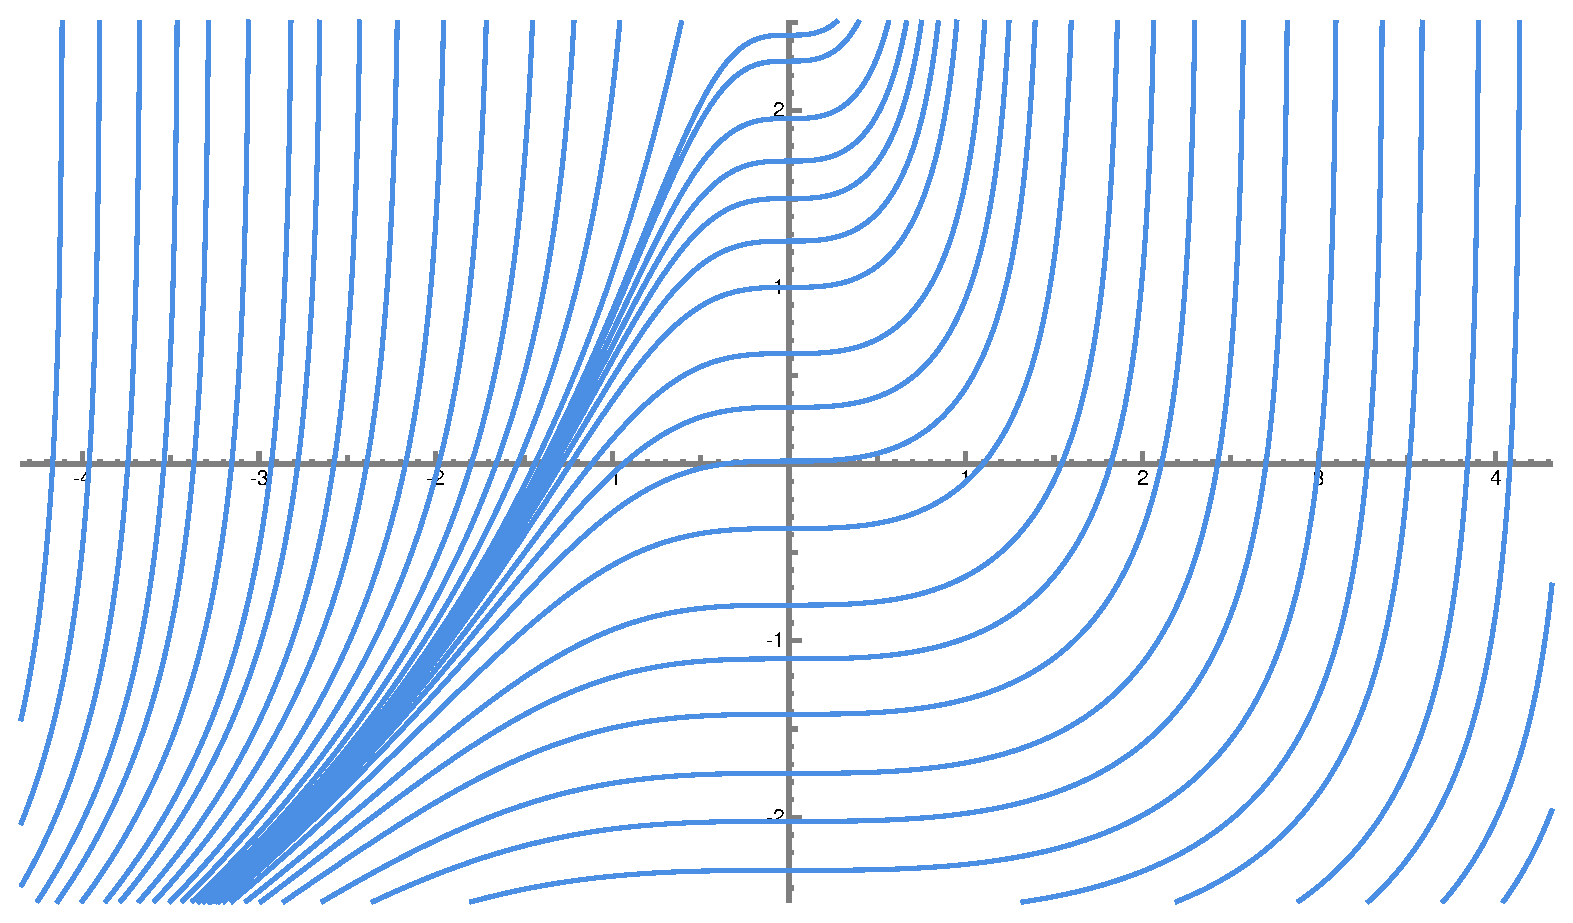
\includegraphics[width=0.8\textwidth]{fig_edo_separabile.pdf}
\caption{i grafici delle soluzioni dell'equazione differenziale~\eqref{eq:separabile}.
Si noti che ogni soluzione ha un asintoto verticale, dunque le singole 
soluzioni non sono definite su tutto $\RR$.
Ma scelto un qualunque punto del piano c'è una soluzione che passa per 
quel punto e inoltre due diverse soluzioni non si incontrano mai.
Queste proprietà sono garantite dal teorema~\ref{th:banach-caccioppoli}.
\ifwidemargin\\\\\fi%
\usebox{\qrseparabile}}
\label{fig:separabile}
\end{figure}

\begin{example}
Risolviamo l'equazione
\begin{equation}\label{eq:43856}
  u' = x u^2 + x.
\end{equation}
\end{example}
%
\begin{proof}[Svolgimento.]
E' una equazione del primo ordine in forma normale.
Raccogliendo $x$ al lato destro si ottiene una equazione a variabili separabili.
Dividendo ambo i membri per $u^2+1$ (che è sempre diverso da zero) si ottiene l'equazione equivalente
\[
\frac{u'}{1+u^2} = x.
\]
Integrando il lato sinistro si ottiene:
\[
  \int \frac{u'(x)}{1+u^2(x)}\, dx
  = \Enclose{\int \frac{du}{1+u^2}}_{u=u(x)}
  \ni \arctg(u(x))
\]
mentre per il lato destro si ottiene
\[
  \int x\, dx \ni \frac{x^2}{2}.
\]
Dunque su ogni intervallo si deve avere
\[
  \arctg(u(x)) = \frac{x^2}{2} + c.
\]
Visto che l'arcotangente assume valori compresi tra $-\pi/2$ e $\pi/2$ anche il lato destro dovrà rimanere in tale intervallo. Dovrà quindi essere:
\begin{equation}\label{eq:4856}
  -\frac \pi 2 < \frac {x^2} 2 + c < \frac \pi 2 .
\end{equation}
Con questa condizione possiamo invertire l'arcotangente ottenendo finalmente una espressione per la soluzione:
\begin{equation}\label{eq:45876314}
  u(x) = \tg\enclose{\frac{x^2}{2} + c}.
\end{equation}

\newsavebox{\qrquattrotre}\sbox{\qrquattrotre}{%
\myqrshortdoclink{43856}{i grafici delle soluzioni dell'equazione differenziale (\getrefnumber{eq:43856})}}
\begin{figure}
\centering
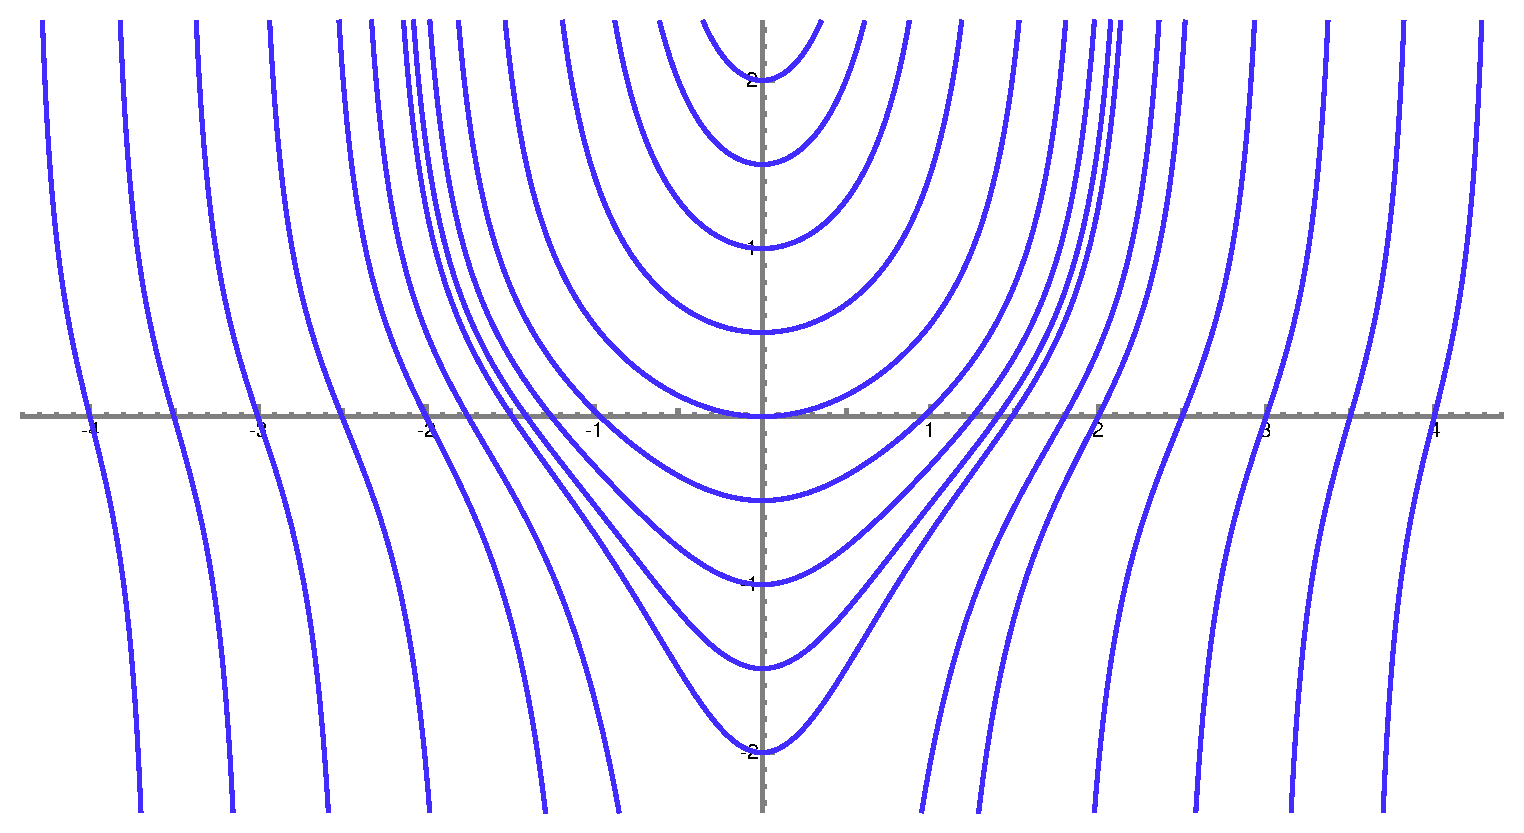
\includegraphics[width=0.8\textwidth]{fig_43856.pdf}
\caption{i grafici delle soluzioni dell'equazione differenziale~\eqref{eq:43856}.
\ifwidemargin\\\\\fi%
\usebox{\qrquattrotre}}
\label{fig:43856}
\end{figure}

Osserviamo che la condizione~\eqref{eq:4856} equivale a richiedere che l'argomento
della tangente stia nell'intervallo $\enclose{-\frac \pi 2, \frac \pi 2}$.
In tal caso dovrà essere $c<\frac\pi 2$ e si osserva che se $c>-\frac \pi 2$
la soluzione $u(x)$ è definita su un intervallo aperto centrato in $x=0$ mentre
se $c \le -\frac \pi 2$ la soluzione è definita su una coppia di intervalli
simmetrici con ampiezza che tende a zero quando $c\to -\infty$.
Agli estremi di tali intervalli la soluzione ha degli asintoti verticali.

In questo caso possiamo osservare che la condizione~\eqref{eq:4856} può essere
trascurata, visto che la funzione $\tg$ è $\pi$-periodica e quindi
è possibile sommare a $c$ un multiplo intero di $\pi$ senza che la soluzione
venga modificata.
Nell'equazione~\eqref{eq:45876314} si potrebbe
quindi considerare la funzione $\tg$
definita su tutto il suo dominio osservando che in tal caso si può
supporre che sia $c\in \left(-\frac \pi 2, \frac \pi 2\right]$.
Invece di ottenere un singolo intervallo per ogni $c$ si ottengono così
tutti gli infiniti intervalli.
\end{proof}

\begin{remark}
L'esempio precedente mette in evidenza il fatto che le soluzioni massimali possono essere definite
su intervalli arbitrariamente piccoli anche se l'equazione differenziale
non presenta singolarità. Diremo in questo caso che
la soluzione non è globale.

D'altra parte si osserva che i grafici delle soluzioni riempiono tutto il piano senza 
mai toccarsi l'uno con l'altro (si dice a volte che sono una \emph{fibrazione}).
Questo è dovuto al fatto che questa equazione soddisfa il 
teorema~\ref{th:cauchy_lipschitz} e quindi per ogni punto 
del piano passa una ed una sola soluzione.
\end{remark}

\begin{example}
Si voglia risolvere l'equazione
\[
  u' = u^2.
\]
Si tratta di una equazione in forma normale, del primo ordine, autonoma.
In particolare è a variabili separabili
$u' = f(u(x))\cdot g(x)$
con $f(u)=u^2$ e $g(x)=1$.
Osserviamo innanzitutto che $u(x) = 0$ è soluzione in quanto $u'(x) = u^2(x) = 0$.
Se $u$ è una soluzione non identicamente nulla ci saranno dei punti in cui
$u(x)\neq 0$.
In un intorno di tali punti possiamo dividere ambo i membri dell'equazione per $u^2(x)$ ottenendo:
\[
  \frac{u'}{u^2} = 1.
\]
Integrando il lato sinistro tramite cambio di variabile $u=u(x)$, $du=u'(x)\, dx$ si ottiene:
\[
  \int \frac{u'(x)}{u^2(x)}\, dx = \Enclose{\int \frac{du}{u^2}}_{u=u(x)} = \Enclose{-\frac{1}{u}}_{u=u(x)}
  = -\frac{1}{u(x)}
\]
mentre integrando il lato destro si ha
\[
  \int 1 \, dx \ni x.
\]
Dunque su ogni intervallo in cui $u(x)\neq 0$ deve esistere una costante $c\in \RR$ tale che
\[
-\frac{1}{u(x)} = x + c
\]
ovvero, ponendo $x_0 = -c$
\begin{equation}\label{eq:5782196}
  u(x) = -\frac{1}{x+c} = \frac{1}{x_0-x}.
\end{equation}

In conclusione abbiamo trovato una soluzione costante $u(x)=0$ e una famiglia
di soluzioni definite sugli intervalli $(-\infty,x_0)$ e $(x_0,+\infty)$
rappresentante dall'equazione~\eqref{eq:5782196}.
Dovremmo ora chiederci
se è possibile che queste soluzioni vengano mescolate tra loro, ovvero
se una soluzione può valere zero in alcune zone e soddisfare~\eqref{eq:5782196}
in altre.

In questo caso la risposta è no.
Basta osservare che una funzione $u$ che soddisfa l'equazione~\eqref{eq:5782196}
può tendere a zero solamente quando $x\to +\infty$ o $x\to -\infty$.
Questo significa che se consideriamo una soluzione $u(x)$
definita su un intervallo $I$ e se in almeno un punto la soluzione è diversa da zero,
allora la soluzione è diversa da zero su tutto $I$ e
soddisfa l'equazione~\eqref{eq:5782196} in quanto la soluzione nulla e la
soluzione \eqref{eq:5782196} non sono tra loro compatibili (non possono essere
incollate con continuità).

Vedremo più avanti un risultato
(proposizione~\ref{prop:separazione_soluzioni})
che garantisce in ipotesi molto generali che due diverse soluzioni non
possono mai incontrarsi.
\end{example}

\begin{exercise}
Fissato $p>1$ si risolva l'equazione differenziale
\[
  u' = u^p
\]
e si osservi che la soluzione presenta sempre un asintoto verticale
(dunque non c'è esistenza globale).
\end{exercise}

\begin{example}[baffo di Peano]
Si determinino tutte le soluzioni del problema di Cauchy
\begin{equation}
\label{eq:94467}
\begin{cases}
  u'(x) = \sqrt[3]{u(x)}\\
  u(0)=0
\end{cases}
\end{equation}
\end{example}
%
\newsavebox{\qrnovequattro}\sbox{\qrnovequattro}{%
\myqrshortdoclink{94467}{Il baffo di Peano formato dalle soluzioni del problema di Cauchy (\getrefnumber{eq:94467})}}
\begin{figure}
\centering
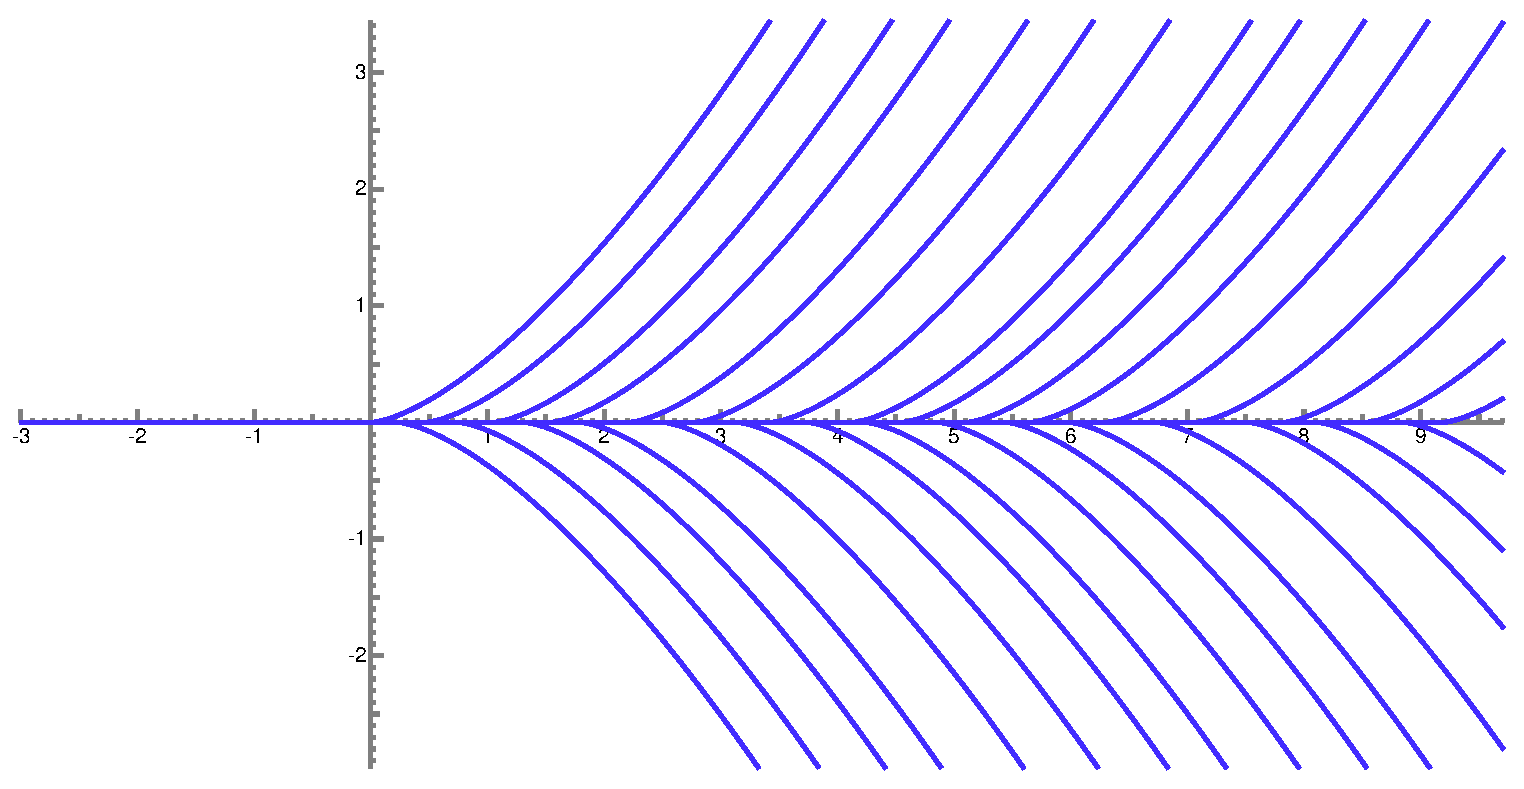
\includegraphics[width=0.9\textwidth]{fig_94467.pdf}
\caption{Il baffo di Peano formato dalle soluzioni del problema di Cauchy~\eqref{eq:94467}.\\\\
\usebox{\qrnovequattro}}
\label{fig:94467}
\end{figure}
%
\begin{proof}[Svolgimento.]
Osserviamo che la funzione nulla $u(x)=0$ è soluzione dell'equazione
e soddisfa la condizione $u(0)=0$.
Ma a priori non possiamo escludere che ci siano altre soluzioni dell'equazione
che verifichino la stessa condizione (vedremo che la
proposizione~\ref{prop:separazione_soluzioni} non si applica in questo caso
particolare).

Nei punti in cui $u(x)\neq 0$ possiamo riscrivere l'equazione nella forma
\[
  \frac{u'(x)}{\sqrt[3]{u(x)}} = 1.
\]
Integrando il lato sinistro tramite il cambio di variabili $u=u(x)$,
$du = u'(x)\, dx$,
si ottiene
\[
  \int \frac{u'(x)}{\sqrt[3]{u(x)}}\, dx
  = \Enclose{\int \frac{du}{\sqrt[3]u}}_{u=u(x)}
  \ni \frac 3 2 \sqrt[3]{u^2(x)}.
\]
integrando anche il lato destro troviamo dunque
che su ogni intervallo su cui $u$ è definita e $u(x)\neq 0$
deve esistere una costante $c$ tale che
\[
  \frac 3 2 \sqrt[3]{u^2(x)} = x + c.
\]
Risolvendo in $u(x)$:
\begin{equation}\label{eq:476937568}
  u(x) = \pm \sqrt{\enclose{\frac 2 3 (x+c)}^3}.
\end{equation}
Osserviamo che la proprietà precedente
può essere soddisfatta solamente se $x\ge -c$ ma affinché
sia $u(x)\neq 0$ dobbiamo imporre $x>-c$.
Ma per $x\to -c^+$
si ha $u(x)\to 0$ e anche $u'(x) = \sqrt[3]{u(x)}\to 0$.
Significa che una soluzione definita su $x>c$ mediante
la~\eqref{eq:476937568} può essere estesa a tutto $\RR$
ponendo $u(x)=0$ per $x\le c$.
Affinché valga la condizione $u(0)=0$ sarà dunque sufficiente
imporre la restrizione $-c\ge 0$.

Il nostro problema ha dunque infinite soluzioni definite
su tutto $\RR$. Per la precisione, per ogni $c\ge 0$
(cambiamo segno alla costante trovata prima, in modo che risulti
positiva)
si hanno le soluzioni
\[
  u(x) = \begin{cases}
    0 & \text{per $x\le c$}\\
    \sqrt{\enclose{\frac 2 3 (x-c)}^3} & \text{per $x>c$}
  \end{cases}
\]
e
\[
  u(x) = \begin{cases}
    0 & \text{per $x\le c$}\\
    -\sqrt{\enclose{\frac 2 3 (x-c)}^3} & \text{per $x>c$}
  \end{cases}
\]
\end{proof}
\subsection{altri metodi risolutivi}

Nella sezione precedente abbiamo visto che le equazioni lineari del primo ordine
e le equazioni
a variabili separabili possono essere ricondotte al calcolo di una primitiva.
Nella sezione~\ref{sec:edo_lineari} verranno esposti i metodi risolutivi per le
equazioni lineari di ordine $n$ a coefficienti costanti.

Ci sono molti altri tipi di equazioni che possono essere ricondotti
alle equazioni lineari o alle equazioni a variabili separabili.
Non potremo dilungarci su questi metodi ma può essere utile,
come riferimento non esaustivo,
un elenco di alcune tipologie di equazioni per le quali esiste un metodo
risolutivo.

\begin{enumerate}
\item \emph{Equazione del secondo ordine senza dipendenza da $u$}
\[
  F(x, u', u'') = 0
\]
si riconduce al primo ordine ponendo $u'(x) = v(x)$, $u''(x) = v'(x)$.

\item \emph{Equazione del secondo ordine autonoma}
\[
  F(u, u', u'') = 0
\]
si riconduce al primo ordine
ponendo $u'(x) = v(u(x))$,
$u''(x) = v'(u(x))\cdot v(u(x))$.

\item \emph{Equazione di Bernoulli}
\index{equazione!di Bernoulli}%
\index{Bernoulli!equazione di}%
\[
  u' = a(x) u + b(x) u^\alpha
\]
si riconduce ad una equazione lineare dividendo tutto per $u^\alpha$
e ponendo $u(x)^{1-\alpha} = v(x)$, $\frac{u'}{u^\alpha} = \frac{v'}{1-\alpha}$.

\item \emph{Equazione di Clairaut}
\index{equazione!di Clairaut}%
\index{Clairaut!equazione di}%
\[
  u = x u' + f(u');
\]
derivando l'equazione si ottiene $ u' = u' + xu'' + f'(u')u''$
che si fattorizza: $u''\cdot(x+f'(u'))=0$. 
Il secondo fattore ci permette di determinare $u'(x)$ e inserendo $u'$
nell'equazione originaria troviamo $u(x)$. 
Il primo fattore $u''=0$ ci dà come soluzione una retta che, sostituendone 
l'equazione nella equazione originaria, scopriamo essere tangente 
alla soluzione trovata precedentemente.
A queste soluzioni bisogna aggiungere le soluzioni non $C^2$ formate da un tratto
della curva inizale e che poi si staccano lungo le semirette tangenti.

\item \emph{equazione di Riccati}
\index{equazione!di Riccati}%
\index{Riccati!equazione di}%
\[
  u' = u^2 + b(x) u + c(x).
\]
si ponga $u(x) = -v'(x)/v(x)$ per ricondursi ad
una equazione lineare del secondo ordine in $v$:
\[
 v'' -  b(x) v' + c v = 0.
\]
\end{enumerate}

\begin{example}[equazione di Newton]
\index{equazione!di Newton}%
\index{Newton!equazione di}%
Un sistema fisico unidimensionale soggetto a forze che dipendono solamente
dalla posizione può essere descritto da un problema di Cauchy:
\[
\begin{cases}
  u''(x) = F(u(x)) \\
  u(x_0) = u_0 \\
  u'(x_0) = v_0
\end{cases}
\]
(ad esempio per il pendolo si ha $F(y) = -\sin y$).
La funzione $v$ definita da $v(u(x)) = u'(x)$ mette in relazione
la velocità con la posizione e descrive quindi il moto nel
cosiddetto \emph{spazio delle fasi}. Con tale sostituzione si
trova
\[
  u''(x) = v'(u(x)) u'(x) = v'(u(x)) v(u(x))
\]
che sostituita in $u'' = F(u)$ ci dà una equazione
differenziale del primo ordine per $v=v(u)$:
\[
 v' v  = F(u).
\]
Questa è una equazione del primo ordine a variabili separabili
che può essere interpretata come la legge di conservazione dell'energia,
infatti è equivalente a
\[
  \frac{d}{dx}\enclose{\frac 1 2 v^2 - \int F(u)} = 0
\]
dove $\frac 1 2 v^2$ si interpreta come energia cinetica e $-\int F$
come energia potenziale.
Integrando tra $x_0$ e $x$ e utilizzando le condizioni iniziali si ottiene,
con $u=u(x)$:
\[
  \frac 1 2 v^2(u) = \frac 1 2 v_0^2 + \int_{u_0}^{u} F(y)\, dy.
\]
Questa equazione descrive la traiettoria del sistema nel piano delle fasi $(u,v)$
e ci permette di ricavare $v$ in funzione di $u$:
\[
  v(u) = \pm\sqrt{v_0^2 + 2\int_{u_0}^u F(u)\, du}
\]
che significa:
\begin{equation}\label{eq:8844475}
  u'(x) = \pm \sqrt{v_0^2 + 2 \int_{u_0}^{u(x)} F(y)\, dy}.
\end{equation}
Questa è una equazione autonoma in $u$, quindi a variabili separabili:
\[
  \pm\frac{u'(x)}{\sqrt{v_0^2 - \int_{u_0}^{u(x)} F(y)\, dy}} = 1
\]
che può essere integrata tra $x_0$ e $x$ facendo il cambio di variabile $u=u(x)$
\[
  \pm\int_{u_0}^{u(x)} \frac{du}{\sqrt{v_0^2-\int_{u_0}^u F(y)\, dy}} = x-x_0.
\]
In questo modo abbiamo determinato la funzione inversa della soluzione $u(x)$.
\end{example}

\begin{example}[periodo del pendolo]
\index{periodo!del pendolo}%
\index{pendolo!periodo del}%
\index{oscillazioni!piccole del pendolo}%
\index{piccole oscillazioni}%
Proviamo a determinare il periodo di oscillazione di un pendolo.
\end{example}
\begin{proof}[Svolgimento.]
Sia $u(x)$
l'angolo di scostamento dalla verticale
al tempo $x$ di un pendolo semplice di lunghezza $\ell$.
Considerando la componente tangenziale della accelerazione di gravità
(il cui modulo è $g$)
l'equazione di Newton può essere scritta nella forma:
\[
  u''(x) = -\frac{g}{\ell} \sin u(x).
\]
Siamo quindi nel caso dell'esempio precedente dove $F(u) = -\frac{g}{\ell} \sin u$
e se al tempo $x=0$ lasciamo cadere da fermo il pendolo da un angolo $u_0$,
si avrà $v_0=0$. L'energia potenziale sarà data allora da
\[
-\frac{g}{\ell}\int_{u_0}^u \sin y\, dy = \frac{g}{\ell}\enclose{\cos u - \cos u_0}.
\]
L'equazione~\eqref{eq:8844475} diventa dunque
\[
  u'(x) = \pm \sqrt{2\frac{g}{\ell}(\cos u(x) - \cos u_0)}.
\]
Separando le variabili e integrando tra $0$ e $x$ si ottiene
\[
\sqrt{\frac \ell g}\int_0^x \frac{u'(t)\, dt}{\pm\sqrt{2\cos u(t)-2\cos u_0}}
= \int_0^x dt  = x.
\]
Cambiando variabile $u=u(x)$, $du = u'(x) dx$:
\begin{equation}\label{eq:4898944}
\sqrt{\frac \ell g}\int_0^{u(x)} \frac{du}{\pm\sqrt{2\cos u-2\cos u_0}} = x.
\end{equation}
La scelta del segno $\pm$ è arbitraria ma visto che $u$ è continua
anche $u''=-\frac g l \sin u$ deve essere una funzione continua. Dunque il segno
$\pm$ può cambiare solo quando $u'=0$. Nel punto iniziale $x=0$ abbiamo
imposto $u'(0) = 0$ e dunque l'energia cinetica è nulla. Visto che l'energia
cinetica non può essere negativa significa che l'energia potenziale
non può aumentare e quindi inizialmente l'angolo $u(x)$ dovrà diminuire
(o almeno: non potrà aumentare). Dunque inizialmente il segno di $u'$ è negativo
e rimarrà negativo finché non si avrà nuovamente $u'(x)=0$.
L'integrale in~\eqref{eq:4898944} è un integrale improprio in quanto
la funzione integranda presenta un asintoto per $u\to u_0^-$ dobbiamo dunque
assicurarci che l'integrale sia finito. Sviluppando $\cos u$ nel punto $u=u_0$
si trova $\cos u = \cos u_0  - \sin u_0 \cdot (u-u_0) + o(u-u_0)$ da cui
\[
 \frac{1}{\sqrt{2 \cos u - 2 \cos u_0}}
 =\frac{1}{\sqrt{2\sin u_0\cdot (u_0-u) + o(u-u_0)}}
 \sim \frac{C}{\sqrt{u_0-u}}
\]
che è notoriamente una funzione integrabile per $u\to u_0^-$.

Vogliamo ora calcolare il tempo $x_1$ in cui il pendolo raggiunge per la prima
volta la verticale, cioè $u(x_1)=0$.
Ricordiamo che al tempo $x=0$ il pendolo parte da un angolo $u_0$
con velocità nulla. Nell'intervallo $x\in[0,x_1]$ si avrà $u'(x)<0$
(l'angolo diminuisce) dunque:
\[
-\sqrt{\frac{\ell}{g}}\int_{u_0}^{0} \frac{du}{\sqrt{2\cos u - 2\cos u_0}}
= x_1.
\]

Una volta raggiunta la verticale, per simmetria il pendolo tornerà a risalire
fino ad un angolo $-u_0$ mettendoci lo stesso tempo $x_1$. Poi tornerà a scendere
e risalire fino a tornare all'angolo $u_0$ mettendoci in totale un tempo
$T=4x_1$ che è quindi il periodo di oscillazione. Si ha dunque
\[
  \frac{T}{4} = \sqrt{\frac \ell g}\int_0^{u_0} \frac{du}{\sqrt{2\cos u - 2\cos u_0}}.
\]

Purtroppo l'integrale che abbiamo trovato non ha una primitiva
esprimibile mediante funzioni elementari (è un integrale ellittico).
Il nostro obiettivo è ora quello di farne uno sviluppo di Taylor
per $u_0\to 0$ che significa determinare
il periodo del pendolo per \emph{piccole oscillazioni}%
\mymargin{piccole oscillazioni}\index{piccole oscillazioni}.

Tramite formule di bisezione possiamo scrivere $\cos u = 1 - 2 \sin^2\frac u 2$
da cui
\[
 \sqrt{2\cos u - 2\cos u_0}
 = \sqrt{4\sin^2 \frac {u_0} 2 - 4 \sin^2 \frac{u}{2}}
 = 2\sin \frac{u_0}2 \sqrt{1-\enclose{\frac{\sin \frac u 2}{\sin \frac {u_0}2}}^2}
\]
dunque ponendo
\begin{equation}\label{eq:4847843}
 \sin t = \frac{\sin \frac u 2}{\sin \frac{u_0} 2}
\end{equation}
si ha
\[
  \sqrt{\frac \ell g} \cdot \frac T 4
  =  \int_0^{u_0} \frac{du}{2\sin \frac {u_0}2 \sqrt{1-\sin^2 t}}
  = \int_0^{u_0} \frac{du}{2\sin \frac{u_0}2 \cos t}
\]
ma per il cambio di variabile~\eqref{eq:4847843} si ha
\[
  \cos t \, dt = \frac{\cos \frac u 2 }{2 \sin \frac{u_0} 2}\, du
\]
ovvero
\[
 \frac{du}{2\sin \frac {u_0} 2 \cos t} = \frac{dt}{\cos \frac u 2}
 = \frac{dt}{\sqrt{1-\sin^2 t \sin^2\frac{u_0}{2}}}
\]
e quindi
\[
\sqrt{\frac g \ell} \cdot \frac{T}{4}
= \int_0^{\frac \pi 2} \frac{dt}{\cos \frac u 2}
= \int_0^{\frac \pi 2} \frac{dt}{\sqrt{1-\sin^2 \frac u 2}}
= \int_0^{\frac \pi 2} \frac{dt}{\sqrt{1-\sin^2 \frac{u_0}{2} \sin^2 t}}.
\]
Utilizzando ora la serie binomiale (teorema~\ref{th:serie_binomiale})
possiamo scrivere
\begin{align*}
\sqrt{\frac g \ell} \cdot\frac{T}{4}
&= \int_0^{\frac \pi 2} \sum_{k=0}^{+\infty}{-\frac 1 2 \choose k} \enclose{-\sin^2 t\sin^2 \frac{u_0}2}^{k}\, dt
\end{align*}
\begin{align*}
&= \int_0^{\frac \pi 2} \sum_{k=0}^{+\infty}\frac{(2k-1)!!}{(2k)!!} \enclose{\sin^2 t\sin^2 \frac{u_0}2}^{k}\, dt
\end{align*}
in quanto si ha
\begin{align*}
  {-\frac 1 2 \choose k}
  &= \frac{\enclose{-\frac 1 2}\cdot \enclose{-\frac 3 2} \cdots \enclose{-\frac{2k-1} 2}}{k!}\\
  &= (-1)^k\frac{(2k-1)!!}{2^k \cdot k!} = (-1)^k \frac{(2k-1)!!}{(2k)!!}.
\end{align*}
Rispetto alla variabile $\sin^2 t$ dentro all'integrale abbiamo ora una serie di potenze
con coefficienti
\[
 a_k = \frac{(2k-1)!!}{(2k)!!} \enclose{\sin^2\frac{u_0} 2}^{k}
\]
e si verifica facilmente che
$  \frac{a_{k+1}}{a_k} \to \sin^2 \frac{u_0}{2}$
dunque la serie di potenze converge se
$ \sin^2 t \le \frac{1}{\sin^2 \frac{u_0}{2}}$
che significa semplicemente
$ \sin \frac u 2 < 1$.
Stiamo quindi facendo un integrale strettamente all'interno 
del raggio
di convergenza della serie. Sappiamo che la serie
converge totalmente e quindi uniformemente su
tale intervallo.
Dunque, applicando il teorema~\ref{th:scambio_limite_integrale} alle somme parziali 
della serie, 
possiamo scambiare la serie con l'integrale:
\[
\sqrt{\frac g \ell} \cdot\frac{T}{4}
= \sum_{k=0}^{+\infty}\frac{(2k-1)!!}{(2k)!!} \enclose{\sin \frac{u_0}2}^{2k}
\int_0^{\frac \pi 2}  \enclose{\sin t}^{2k}\, dt
\]
l'integrale è ora sostanzialmente lo stesso $I_n$ che abbiamo 
calcolato nel teorema~\ref{th:wallis}:
\[
  \int_0^{\frac \pi 2} \enclose{\sin t}^{2k}\, dt
  = \frac 1 2 \int_0^{\pi} \enclose{\sin t}^{2k}\, dt
  = \frac{I_{2k}}{2}
  = \frac \pi 2 \cdot\frac{(2k-1)!!}{(2k)!!}
\]
da cui
\[
T
= 2\pi\sqrt{\frac \ell g}\sum_{k=0}^{+\infty} \enclose{\frac{(2k-1)!!}{(2k)!}}^2
\enclose{\sin \frac{u_0} 2}^{2k}.
\]

Possiamo allora cercare di scrivere i primi termini dello sviluppo di
Taylor di $T = T(u_0)$ per $u_0\to 0$ diciamo, per esempio, fino all'ordine 8
in $u_0$. Basterà considerare la somma dei termini della
serie per $k=0,1,2,3,4$ in quanto la somma dei termini per $k\ge 5$ mi darà
 un contributo dell'ordine di $O\enclose{\sin \frac {u_0} 2}^{10} = o(u_0^8)$. Dunque
 \begin{align*}
 \sqrt{\frac{g}{\ell}}\cdot \frac{T}{2\pi}
 &=
 1 + \enclose{\frac 1 2}^2 \sin^2 \frac{u_0} 2
 + \enclose{\frac{1\cdot 3}{2\cdot 4}}^2\enclose{\sin^2 \frac {u_0} 2}^2 \\
 &\quad + \enclose{\frac{1\cdot 3 \cdot 5}{2\cdot 4 \cdot 6}}^2
 \enclose{\sin^2 \frac {u_0} 2}^3 + \enclose{\frac{1\cdot 3\cdot 5 \cdot 7}{2\cdot 4\cdot 6\cdot 8}}^2
 \enclose{\sin^2 \frac {u_0} 2}^4 + o(u_0^8) \\
%\end{align*}
%\begin{align*}
 &=
1 + \frac 1 4 \enclose{\frac{u_0^2}{4} - \frac{u_0^4}{2^4\cdot 3} + \frac{u_0^6}{2^5\cdot 3^2\cdot 5}
- \frac{u_0^8}{2^8\cdot 3^2\cdot 5\cdot 7}} \\
&\quad + \frac{3^2}{2^6}\enclose{\frac{u_0^2}{4} - \frac{u_0^4}{2^4\cdot 3}
+ \frac{u_0^6}{2^5\cdot 3^2\cdot 5}}^2\\
&\quad + \frac{5^2}{2^8}\enclose{\frac{u_0^2}{4} - \frac{u_0^4}{2^4\cdot 3}}^3
+ \frac{5^2\cdot 7^2}{2^{14}}
\frac {u_0^8} {2^8} + o(u_0^8)\\
%\end{align*}
%\begin{align*}
&=
1 + \frac{u_0^2}{2^4} - \frac{u_0^4}{2^6\cdot 3} + \frac{u_0^6}{2^7\cdot 3^2\cdot 5}
- \frac{u_0^8}{2^{10}\cdot 3^2\cdot 5\cdot 7} \\
&\quad + \frac{3^2}{2^6}\enclose{\frac{u_0^4}{2^4} - \frac{u_0^6}{2^5\cdot 3} + \frac{u_0^8}{2^8\cdot 3^2} + \frac{u_0^8}{2^6\cdot 3^2\cdot 5}}\\
&\quad + \frac{5^2}{2^8}\enclose{\frac{u_0^6}{2^6} - \frac{u_0^8}{2^8}}
+ \frac{5^2\cdot 7^2}{2^{22}}
u_0^8 + o(u_0^8)\\
%
% \end{align*}
% \begin{align*}
&= 1 + \frac{u_0^2}{2^4} + \frac{11}{2^{10}\cdot 3} u_0^4
 + \frac{173}{2^{14}\cdot 3^2\cdot 5} u_0^6
 + \frac{22931}{2^{22}\cdot 3^2\cdot 5\cdot 7} u_0^8
 + o(u_0^8).\\
\end{align*}
\end{proof}

%%%%%%%%%%%%%%%%%%%%
%%%%%%%%%%%%%%%%%%%%
%%%%%%%%%%%%%%%%%%%%
\section[funzioni vettoriali e di più variabili]{alcuni risultati preparatori
sulle funzioni vettoriali e di più variabili}
%%%%%%%%%%%%%%%%%%%%
%%%%%%%%%%%%%%%%%%%%
%%%%%%%%%%%%%%%%%%%%

Ci sarà utile estendere la definizione delle classi di regolarità $C^k$ alle
funzioni vettoriali (cioè con codominio $\RR^n$) e di più variabili
(cioè con dominio $\RR^m$).

\subsection{continuità e compattezza}

Lo spazio $\RR^n$ è uno spazio metrico con la distanza euclidea 
(definizione~\ref{def:124124})
$d(\vec x, \vec y) = \abs{\vec x- \vec y}$ con 
\[
 \abs{\vec x} = \sqrt{x_1^2 + \dots + x_n^2}.  
\] 

Dunque una successione $\vec x_k\in \RR^n$ converge 
ad un punto $\vec p\in \RR^n$ se vale 
(definizione~\ref{def:convergenza_metrica}) 
$\abs{\vec x_k - \vec p}\to 0$.
Se $(x_k)_j$ sono le componenti del punto $\vec x_k\in \RR^n$ e 
$p_j$ sono le componenti di $\vec p\in \RR^n$ la convergenza 
$\vec x_k \to \vec p$ è equivalente alla convergenza di 
tutte le componenti: $(x_k)_j \to p_j$ per ogni $j=1,\dots,n$
per $k\to +\infty$.

Una funzione $\vec f\colon A \subset \RR^n\to \RR^m$ 
è \emph{continua} 
(definizione~\ref{def:continua_metrico})
se per ogni successione $\vec x_n \to \vec p$ con 
$\vec x_n\in A$ e $\vec p\in A$ risulta 
\[
  \vec f(\vec x_n) \to \vec f(\vec p).
\]

Un insieme $K\subset \RR^n$ è \emph{chiuso}%
\mymargin{chiuso}\index{chiuso}
se presa una qualunque successione convergente in $\RR^n$:
$\vec x_k \to \vec x$ se ogni $\vec x_k\in K$ allora anche 
$\vec x \in K$ (cioè $K$ è chiuso per passaggio al limite,
teorema~\ref{th:chiuso_sequenziale}).
La palla di raggio $r>0$ centrata nel punto $\vec p\in \RR^n$ 
è l'insieme (definizione~\ref{def:palla}):
\[
  B_r(\vec p) = \ENCLOSE{\vec x \in \RR^n\colon \abs{\vec x - \vec p}< r}.  
\]
Un insieme $\Omega\subset \RR^n$ è \emph{aperto}
se per ogni $\vec p\in \Omega$ esiste $r>0$ tale che $B_\rho(\vec p) \subset \Omega$
(definizione~\ref{def:466342}).
Un insieme $B\subset \RR^n$ si dice essere \emph{limitato}
(definizione~\ref{def:spazio_limitato})
se esiste $r>0$ e $\vec p\in\RR^n$ tali che $B\subset B_r(\vec p)$ 
(ma non è restrittivo supporre $\vec p=0$).
Un insieme $K\subset \RR^n$ si dice essere \emph{compatto} 
(definizione \ref{def:sequenzialmente_compatto}) se da ogni successione 
$\vec x_k$ di punti di $K$ è possibile estrarre una sottosuccessione $x_{k_j} \to \vec x$ 
convergente ad un punto $\vec x \in K$.
In $\RR^n$ un insieme è compatto se e solo se è chiuso e limitato
(teorema~\ref{th:compattezza_Rn}).
Una funzione continua $f\colon K\subset \RR^n\to\RR$ definita
su un compatto $K$ è limitata per il teorema di Weierstrass (teorema~\ref{th:weiestrass_metrico}).


\subsection{derivate parziali}

Se $\Omega\subset \RR^m$ è un insieme aperto e $f\colon \Omega \to \RR$
è una funzione, vogliamo definire le \emph{derivate parziali} di $f$.
Se $\vec x \in \Omega$ si ha $\vec x = (x_1,\dots, x_m)$ e quindi
$f(\vec x) = f(x_1,\dots, x_m)$. Se facciamo variare una sola componente
$x_j$ mantenendo fisse tutte le altre componenti, otteniamo una funzione
di una variabile $x_j \mapsto g(x_j) = f(x_1,\dots, x_j, \dots, x_m)$.
Definiamo dunque la \emph{derivata parziale}
\mymargin{derivata parziale}
\index{derivata!parziale}
di $f$ rispetto alla variabile $x_j$ come la derivata della funzione $g(x_j)$.
Denotiamo tale derivata con il simbolo:
\[
  \frac{\partial f}{\partial x_j}.
\]
Le derivate parziali si calcolano dunque come le usuali derivate per le
funzioni di una variabile, solamente bisogna considerare costanti tutte
le variabili tranne quella coinvolta nella derivazione.
Ad esempio se $f(x,v) = -\sin(x) - v$
(come nell'esempio fatto nell'introduzione) si ha
\begin{align*}
  \frac{\partial f}{\partial x} &= -\cos(x)\\
  \frac{\partial f}{\partial v} &= -1.
\end{align*}

Se $\vec f\colon \Omega \subset \RR^m \to \RR^n$ è una funzione di più
variabili a valori vettoriali potremo scrivere $\vec f = (f_1, \dots, f_n)$
e considerare le derivate parziali di ogni componente:
\[
  \frac{\partial \vec f}{\partial x_j}
  = \enclose{\frac{\partial f_1}{\partial x_j}, \dots, \frac{\partial f_n}{\partial x_j}}.
\]

\begin{definition}
Sia $\Omega\subset \RR^m$ un aperto. Denoteremo con $C^0(\Omega,\RR^n)$
lo spazio vettoriale di tutte le funzioni
continue $f\colon \Omega \to \RR^n$.

Denotiamo con $C^1(\Omega,\RR^n)$ lo spazio vettoriale
delle funzioni in $C^0(\Omega,\RR^n)$ tali che ognuna delle loro derivate
parziali $\frac{\partial f}{\partial x_j}$ esiste in ogni punto di $\Omega$ ed
è a sua volta una funzione continua (cioè in $C^0(\Omega,\RR^n)$).
Ricorsivamente si definisce $C^k(\Omega,\RR^n)$ per $k>1$,
come lo spazio delle funzioni $\Omega\to\RR^n$ tali che tutte le loro derivate
parziali stanno in $C^{k-1}(\Omega,\RR^n)$.

Quando lo spazio di arrivo non è indicato si sottointende sempre $\RR$, quindi
$C^k(\Omega) = C^k(\Omega,\RR)$.
\end{definition}

\begin{theorem}[stabilità delle funzioni regolari]
Sia $\Omega \subset \RR^n$ un aperto.
Se $f,g\in C^k(\Omega)$ allora anche $f+g$, $f-g$, $f\cdot g$ e $\frac{f}{g}$
(dove è definita) sono di classe $C^k$. Se $f\in C^k(\Omega)$ e $g\in C^k(\RR)$
allora $g\circ f \in C^k(\Omega)$.
\end{theorem}
%
\begin{proof}
Il fatto che la composizione di funzioni continue sia una funzione continua
è vero in generale in qualunque spazio metrico.
Infatti se $f\colon X\to Y$ e $g\colon Y \to Z$ e se $x_k\to x$ in $X$
allora $f(x_k) \to f(x)$ in $Y$ (per la continuità di $f$)
e quindi $g(f(x_k)) \to g(f(x))$ in $Z$ (per la continuità di $g$).
Dunque $(g \circ f)(x_k) \to (g\circ f)(x)$ e $g\circ f\colon X\to Z$ è continua.

Possiamo dunque osservare che le funzioni di due variabili $s(x,y) = x+y$,
$d(x,y)=x-y$ e
$m(x,y)=xy$ sono funzioni continue da $\RR^2\to \RR$ 
(grazie al teorema~\ref{th:operazioni_limiti}). 
Questo garantisce
che la somma, la differenza e il prodotto di funzioni continue siano funzioni continue.
Anche il reciproco di funzioni continue è una funzione continua
in quanto la funzione $r(x)=1/x$ è continua.
Ne consegue che il rapporto di funzioni continue è una
funzione continua.

Veniamo ora alle derivate parziali.
Per le regole di derivazione delle funzioni di una variabile sappiamo che
somma, prodotto, differenza, rapporto (ove definito) e composizione
di funzioni derivabili sono
a loro volta funzioni derivabili e la derivata si esprime sempre mediante
somma, prodotto, differenza e rapporto delle funzioni coinvolte e delle loro
derivate. Dunque quello che si ottiene combinando tra loro funzioni
di classe $C^k$ è una funzione continua le cui derivate parziali esistono e
sono di classe $C^{k-1}$, dunque è una funzione di classe $C^k$.
\end{proof}

\subsection{integrali di funzioni vettoriali}

\begin{definition}
Sia $\vec f\colon [a,b]\to \RR^m$, $\vec f(x) = (f_1(x), \dots, f_m(x))$.
Diremo che $\vec f$ è integrabile su $[a,b]$ se ogni
$f_k\colon[a,b]\to \RR$ è integrabile su $[a,b]$ e in tal caso porremo:
\[
  \int_a^b \vec f(x)\, dx
  = \enclose{\int_a^b f_1(x)\, dx, \dots, \int_a^b f_m(x)\, dx}
  \in \RR^m
\]
cosicché per ogni $k=1,\dots, m$ si ha:
\[
  \enclose{\int_a^b \vec f(x)\, dx}_k = \int_a^b f_k(x)\, dx.
\]
Come al solito si pone inoltre $\int_b^a \vec f = - \int_a^b \vec f$.
\end{definition}

\begin{theorem}\label{teo:tipo_jensen}
\label{th:stima_modulo_integrale}%
\mymark{*}%
Sia $\vec f\colon [a,b]\to \RR^m$ integrabile. Allora si ha
\[
  \abs{\int_a^b \vec f(x)\, dx} \le \int_a^b \abs{\vec f(x)}\, dx.
\]
\end{theorem}
%
\begin{proof}
Posto
\[
 \vec v = \int_a^b \vec f(x)\, dx
\]
si ha, usando la linearità dell'integrale
e sfruttando la disuguaglianza di Cauchy-Schwarz
\begin{align*}
  \abs{\vec v}^2
  &= \vec v \cdot \vec v
   = \sum_{k=1}^m v_k \int_a^b f_k(x)\, dx
   = \int_a^b \sum_{k=1}^m v_k f_k(x)\, dx \\
  &= \int_a^b \enclose{\vec v, \vec f(x)}\, dx
  \le \int_a^b \abs{\vec v}\cdot \abs{\vec f(x)}\, dx
  = \abs{\vec v} \int_a^b \abs{\vec f(x)}\, dx.
\end{align*}
Se $\abs{\vec v}\neq 0$ possiamo dividere ambo i membri per $\abs{\vec v}$ e
ottenere la disuguaglianza cercata.
Altrimenti se $\abs{\vec v}=0$ la disuguaglianza è certamente soddisfatta in
quanto il lato destro non può essere negativo.
\end{proof}


%%%%%
%%%%%
%%%%%
%%%%%

\section{il problema di Cauchy}
%%%%%
%%%%%
%%%%%
%%%%%

Il problema di Cauchy per i sistemi del primo ordine
consiste nel
trovare una soluzione di un sistema di 
$n$ equazioni differenziali ordinarie del primo ordine in $n$ incognite
$u_1, \dots, u_n$
con un dato iniziale fissato. 
Cioè dato $x_0\in \RR$,
e $\vec y_0 \in \RR^n$ si cerca un intervallo $I\subset \RR$ con $x_0\in I$ 
e una funzione $\vec u \colon I\to \RR^n$,
$\vec u = (u_1, \dots, u_n)$, tale
che $\vec u$ sia derivabile e soddisfi:
\begin{equation}\label{eq:problema_cauchy}
\begin{cases}
 \vec u'(x) = \vec f(x, \vec u(x)), \qquad \forall x\in I\\
 \vec u(x_0) = \vec y_0.
\end{cases}
\end{equation}

\subsection{esistenza e unicità locale}

\begin{theorem}[Cauchy-Lipschitz: esistenza e unicità locale]%
  \label{th:cauchy_lipschitz}%
  \index{Cauchy!teorema di Cauchy-Lipschitz}%
  \index{teorema!di Cauchy-Lipschitz}%
  \index{teorema!di esistenza e unicità locale}%  
Siano $a\le x_0 \le b$, $R>0$, $\vec y_0 \in \RR^n$. 
Posto $K=\ENCLOSE{\vec y\in \RR^n \colon \abs{\vec y - \vec y_0}\le R}\subset \RR^n$ 
sia $\vec f\colon [a,b]\times K\to \RR^n$ una funzione con le proprietà:
\begin{enumerate}
  \item $\vec f$ è continua,
  \item esiste $L>0$ tale che per ogni $x\in [a,b]$, ed ogni $\vec y_1,\vec y_2 \in K$ 
  si ha 
  \begin{equation}\label{eq:hp_lipschitz}
  \abs{\vec f(x, \vec y_2) - \vec f(x,\vec y_1)} \le L \abs{\vec y_2- \vec y_1}.  
  \end{equation}
\end{enumerate}

Allora esiste $\delta>0$ tale che posto 
scelto comunque un intervallo $I$ con 
$x_0 \in I \subset [a,b]\cap [x_0-\delta, x_0+\delta]$ 
esiste una unica funzione derivabile $\vec u\colon I \to K$ 
che risolve il problema di Cauchy~\eqref{eq:problema_cauchy}.
\end{theorem}
%
\begin{proof}
  \emph{Passo 1.}
  Per prima cosa vogliamo dimostrare che una funzione $\vec u\colon I\to K\subset \RR^n$
  è derivabile e risolve il problema di Cauchy~\eqref{eq:problema_cauchy} 
  se e solo se 
  $\vec u$ è continua e risolve l'equazione integrale
  \begin{equation}\label{eq:problema_cauchy_integrale}
  \vec u(x) = \vec y_0 + \int_{x_0}^x \vec f(t,\vec u(t))\, dt.
  \end{equation}

  Se $\vec u$ è derivabile e 
  $\vec u'(x) = \vec f(x, \vec u(x))$ per ogni $x\in I$ allora 
  siccome $\vec f$ è continua la funzione $\vec f(t,\vec u(t))$ è continua 
  (teorema~\ref{th:continuita_funzione_composta_metrico})
  e quindi $\vec u$ è di classe $C^1$. 
  Posso allora integrare ambo i membri 
  e ottenere:
  \[
   \int_{x_0}^x \vec u'(t)\, dt = \int_{x_0}^x \vec f(t,\vec u(t))\, dt.  
  \]
  Per il teorema fondamentale del calcolo il lato sinistro è uguale 
  a $\vec u(x) - \vec u(x_0) = \vec u(x) - \vec y_0$ e quindi si ottiene 
  la validità di~\eqref{eq:problema_cauchy_integrale}.

  Viceversa se $\vec u$ è continua e soddisfa~\eqref{eq:problema_cauchy_integrale}
  allora, sempre per il teorema fondamentale del calcolo possiamo affermare
  che l'integrale nel lato destro nell'uguaglianza~\eqref{eq:problema_cauchy_integrale}
  è una funzione derivabile con derivata $\vec f(x,\vec u(x))$ e dunque anche 
  il lato sinistro è derivabile e vale $\vec u'(x) = \vec f(x,\vec u(x))$ per 
  ogni $x\in I$. 
  Abbiamo già osservato che se $\vec u$ è continua questa funzione (che è la derivata 
  di $\vec u$) è anch'essa continua e quindi $\vec u$ è di classe $C^1$.
  Per $x=x_0$ l'integrale si annulla e quindi si ottiene 
  anche $\vec u(x_0) = \vec y_0$ concludendo che in effetti $\vec u$ risolve 
  il problema di Cauchy~\eqref{eq:problema_cauchy}.

  \emph{Passo 2.}
  Visto che $[a,b]\times K$ è un insieme chiuso e limitato in $\RR \times \RR^n$ 
  il teorema di Weierstrass garantisce che esiste $M>0$ tale che 
  $\abs{\vec f(x,y)}\le M$ per ogni $x\in [a,b]$ e ogni $y\in K$.
  Scegliamo $\delta >0$ tale che $\delta \le \frac{R}{M}$ e $\delta < \frac {1}{L}$
  e prendiamo l'intervallo $I = [a,b]\cap [x_0-\delta,x_0+\delta]$.
  Consideriamo ora l'insieme $X=C(I,K)\subset C(I,\RR^n)$ di tutte le funzioni continue $\vec u\colon I\to K$
  e mettiamo su $X$ la distanza uniforme $d_\infty$.
  E' facile osservare che $X$ è un sottospazio chiuso di $\B(I,\RR^n)$ (le funzioni limitate definite su $I$)
  e visto che quest'ultimo è uno spazio completo (teorema~\ref{th:limitate_completo}) anche $X$ 
  è completo (teorema~\ref{th:chiuso_completo}).

  Definiamo su $X$ l'operatore $T\colon X \to C(I,\RR^n)$ come segue:
  \[
    T(\vec u)(x) = \vec y_0 + \int_{x_0}^x \vec f(t,\vec u(t))\, dt.
  \]
  Osserviamo che l'equazione~\eqref{eq:problema_cauchy_integrale} può essere riscritta
  come equazione di punto fisso: $T(\vec u) = \vec u$. 
  Il nostro intento è quindi quello di utilizzare il teorema~\ref{th:banach-caccioppoli} delle contrazioni.

  \emph{Passo 3.}
  Dimostriamo innanzitutto che $T(X)\subset X$ cosicché possiamo pensare a $T$ come ad un operatore 
  $T\colon X\to X$ che manda $X$ in sé.
  Posto $\vec v = T(\vec u)$ si ha
  (teorema~\ref{th:stima_modulo_integrale}):
  \begin{align*}
    \abs{\vec v(x)-\vec y_0} 
    &= \abs{\int_{x_0}^x \vec f(t, \vec u(t))\, dt} 
    \le \abs{\int_{x_0}^x \abs{\vec f(t,\vec u(t))}\, dt}\\
    &\le \abs{\int_{x_0}^x M\, dt } 
    = \abs{x-x_0}\cdot M \le \delta \cdot M.
  \end{align*}
Visto che abbiamo scelto $\delta \le \frac{R}{M}$ si ottiene che $v(x) \in K$ per ogni $x\in I$ 
e quindi effettivamente $T(u)\in K$.

\emph{Passo 4.}
Dimostriamo infine che $T$ è una contrazione. 
Se $\vec u,\vec v\in X$ si ha, usando l'ipotesi~\eqref{eq:hp_lipschitz} con $x=t$, $\vec y_1=\vec u(x)$
$\vec y_2 = \vec v(x)$,
\begin{align*}
\abs{T(\vec u)(x)-T(\vec v)(x)} 
  &= \abs{\int_{x_0}^x \vec f(t,\vec u(t))\, dt - \int_{x_0}^x \vec f(t,\vec v(t))\, dt} \\
  &\le \abs{\int_{x_0}^x \abs{\vec f(t,\vec u(t))- \vec f(t,\vec v(t))}\, dt }\\
  &\le \abs{\int_{x_0}^x L\cdot  \abs{\vec u(t) - \vec v(t)}\, dt} 
  \le \abs{\int_{x_0}^x L \cdot d_\infty(\vec u, \vec v)\, dt}  \\
  &=\abs{x-x_0}\cdot L \cdot d_\infty(\vec u,\vec v)
  \le \delta \cdot L \cdot d_\infty(\vec u,\vec v).
\end{align*}
Avendo scelto $\delta < \frac{1}{L}$ si ha $\delta L<1$ e quindi effettivamente l'operatore $T$ 
è una contrazione.
Sono dunque verificare le ipotesi del teorema~\ref{th:banach-caccioppoli} delle contrazioni
che garantiscono l'esistenza e unicità del punto fisso $\vec u$.

Ma abbiamo già osservato che $T(\vec u) = \vec u$ è equivalente al problema di Cauchy~\eqref{eq:problema_cauchy}
e quindi la dimostrazione è terminata.
\end{proof}

\begin{definition}[Cauchy-Lipschitz]%
\label{def:cauchy_lipschitz}%
Diremo che una funzione $\vec f\colon \Omega\subset \RR\times \RR^n \to \RR^m$
soddisfa la \emph{proprietà di Cauchy-Lipschitz}%
\mymargin{proprietà di Cauchy-Lipschitz}\index{proprietà di Cauchy-Lipschitz} se $f$ è continua e se
per ogni $(x_0,\vec y_0)\in \Omega$ esistono $a<x_0$, $b>x_0$, $R>0$ ed $L>0$
tali che le ipotesi del teorema~\ref{th:cauchy_lipschitz} sono verificate.
\end{definition}
 
La condizione di Cauchy-Lipschitz può sembrare piuttosto complicata
da verificare. Una condizione molto più semplice  è che la funzione $\vec f$
sia di classe $C^1$. La seguente proposizione ci dice che tale
condizione è sufficiente per applicare il teorema di Cauchy-Lipschitz.

\begin{proposition}%
\mymark{***}%
Sia $\Omega \subset \RR\times \RR^n$ un insieme aperto.
Se $\vec f\in C^1(\Omega,\RR^m)$ 
allora $f$ soddisfa la condizione
di Cauchy-Lipschitz (definizione~\ref{def:cauchy_lipschitz}).

In particolare, grazie al teorema~\ref{th:cauchy_lipschitz} 
per ogni $(x_0,\vec y_0)\in \Omega$ esiste un intervallo aperto 
$I$ contenente il punto $x_0$
ed esiste una unica soluzione $u$ 
del problema di Cauchy~\eqref{eq:problema_cauchy} definita 
su tale intervallo $I$.
\end{proposition}
%
\begin{proof}
\mymark{***}%
Se prendiamo un qualunque cilindro $[a,b]\times K$ con 
\[
  K=\ENCLOSE{\vec y\in \RR^n\colon \abs{\vec y-\vec y_0}\le R}, 
\]
$\vec y_0\in \Omega$, $K\subset \Omega$
sappiamo che ogni derivata parziale
$\partial f_k / \partial y_j$ è continua ed è quindi limitata
(per il teorema di Weierstrass) su $[a,b]\times K$. 
Sia $L_{k,j}$ il massimo di $\abs{\partial f_k / \partial y_j}$ su $K$ e sia
$L$ il massimo degli $L_{k,j}$ per $k=1,\dots m$ e $j=1\dots,n$.
Allora presi $\vec y, \vec z\in K$ si può scomporre l'incremento vettoriale 
$\vec z - \vec y$ lungo le $n$ direzioni coordinate e applicare il teorema di Lagrange lungo ogni direzione.
Per ogni $k = 1,\dots, m$ si ha quindi:
\begin{align*}
\MoveEqLeft
\abs{f_k(x,\vec z)-f_k(x,\vec y)}\\
&\le \sum_{j=1}^n \abs{f_k(x,z_1, \dots, z_j, y_{j+1}, \dots, y_n) - f_k(x,z_1, \dots, z_{j-1}, y_j, \dots, y_n)}\\
&\le \sum_{j=1}^n L_{k,j} \abs{z_j-y_j}
\le \sum_{j=1}^n L_{k,j} \abs{\vec z-\vec y}
\le n L \abs{\vec z-\vec y}
\end{align*}
da cui
\begin{align*}
  \abs{\vec f(x,\vec z) - \vec f(x,\vec y)}
  &= \sqrt{\sum_{k=1}^m \abs{f_k(x,\vec z) - f_k(x,\vec y)}^2} 
  \le \sqrt{\sum_{k=1}^m n^2 L^2 \abs{\vec z-\vec y}^2} \\
  &\le n\sqrt{m} L \abs{\vec z-\vec y} = L' \abs{\vec z-\vec y}.
\end{align*}
\end{proof}

Il teorema di Cauchy-Lipschitz garantisce l'esistenza di una soluzione
definita in un
piccolo intervallo $[x_0-\delta_0, x_0+\delta_0]$ intorno al punto iniziale $x_0$.
Se scegliamo $x_1 = x_0+\delta_0$ possiamo applicare nuovamente lo stesso
teorema per trovare una soluzione definita nell'intervallo
$[x_1, x_1+\delta_1]$
che coincida con la precedente soluzione nel punto $x_1$.
Le due soluzioni possono
essere incollate per ottenere una soluzione definita sull'unione dei due intervalli.
Questo procedimento può essere ripetuto infinite volte ma gli intervalli
potrebbero diventare sempre più piccoli, quindi non c'è garanzia di ottenere una
soluzione definita su intervalli sempre più grandi.
Nel seguito cercheremo di capire quanto grande può essere l'intervallo
\emph{massimale} su cui si riesce ad estendere la soluzione.

\begin{definition}[soluzione/intervallo massimale]
Sia $I\subset \RR$ un intervallo non vuoto e sia $\vec u \colon I \to \RR^n$
una soluzione di una equazione differenziale.

Se $J\supset I$, $J \neq I$ è un intervallo, se $\vec v\colon J \to \RR^n$
risolve la stessa equazione differenziale
e se $\vec v(x)=\vec u(x)$ per ogni $x\in I$,
diremo che $\vec v$ è una \emph{estensione della soluzione}%
\mymargin{estensione della soluzione}\index{estensione della soluzione} $u(x)$.

Se la soluzione $\vec u$ non ammette estensioni, diremo che $\vec u$ è una
soluzione definita su un intervallo massimale o, più semplicemente, diremo
che $\vec u$ è una \emph{soluzione massimale}%
\mymargin{soluzione massimale}\index{soluzione massimale}.
\end{definition}

\begin{proposition}[caratterizzazione delle soluzioni massimali]
\label{prop:edo_massimale}
Sia $\Omega \subset \RR\times \RR^n$ un insieme aperto
e supponiamo che $\vec f\colon \Omega\subset \RR\times\RR^n\to\RR^n$
sia una funzione continua che soddisfa la condizione
di Cauchy-Lipschitz (definizione~\ref{def:cauchy_lipschitz}).
Allora una soluzione $\vec u$ dell'equazione
\begin{equation}\label{eq:edo_normale_ordine_uno}
  \vec u'(x) = \vec f(x, \vec u(x))
\end{equation}
definita su un intervallo $I$ è massimale se e solo se
$I$ è aperto e per ogni $K$ compatto $K\subset \Omega$
e per ogni $x_0 \in I$ esistono $x_1,x_2\in I$, $x_1 < x_0 < x_2$ tali che 
$(x_1, \vec u(x_1))\not \in K$ e $(x_2,\vec u(x_2)) \not \in K$.
Significa cioè che il grafico di $\vec u$ cioè la curva $(x,\vec u(x))$ esce da qualunque compatto  
$K\subset \Omega$ sia facendo crescere $x$ verso destra che facendo calare $x$ verso sinistra.
Intuitivamente il grafico della soluzione massimale tende ad arrivare ai limiti di $\Omega$.
\end{proposition}
%
\begin{proof}
\emph{Prima implicazione}.
Supponiamo che $\vec u\colon I \to \RR^n$ sia una soluzione di~\eqref{eq:edo_normale_ordine_uno} 
definita su un intervallo massimale $I$. Dovrà essere $(x,\vec u(x))\in \Omega$ per ogni $x\in I$.

Mostriamo innanzitutto
che $I$ è un intervallo aperto a destra: se non lo fosse si avrebbe che $x_0=\sup I \in I$. 
Allora $(x_0,\vec u(x_0))\in \Omega$ e per il teorema di esistenza e unicità locale
potremmo trovare un piccolo intervallino $J=[x_0,x_0+\delta]$ una funzione
$\vec v\colon J\to \RR^n$ che risolve~\eqref{eq:edo_normale_ordine_uno}
con $\vec v(x_0)=\vec u(x_0)$.
Facendo l'unione dei due grafici ottengo una estensione di $\vec u$ a tutto l'intervallo
$I\cup J$ che è strettamente più grande di $I$. 
Dunque $\vec u$ non poteva essere una soluzione massimale.

Mostriamo ora che la curva $(x,\vec u(x))$ esce da ogni compatto $K\subset \Omega$ sia da destra che da sinistra. 
Supponiamo per assurdo che esista un compatto $K$ tale che $(x,\vec u(x))\in K$ per ogni $x\in I$.
Il grafico $(x,\vec u(x))$ è limitato per $x\in I$ dunque certamente $I$ deve essere limitato. 
Inoltre abbiamo visto che $I$ è aperto e quindi $I=(a,b)$ con $a,b\in \RR$, $a<b$.

Allora per ogni $x\in I=(a,b)$ si ha
\[
  \abs{\vec u'(x)} = \abs{\vec f(x, \vec u(x))}
   \le \sup_K \abs{\vec f}.
\]
Visto che $\vec f$ è continua 
la funzione $\abs{\vec f}$ ha massimo su $K$ per il teorema di Weierstrass 
e quindi la funzione limitata $\vec u$ ha derivata $\vec u'(x)=\vec f(x,\vec u(x))$ 
anch'essa limitata. 
Si può quindi applicare l'esercizio~\ref{ex:estensione_continua_derivata_limitata}
oppure il teorema~\ref{th:estensione_uniformemente_continua} 
(avendo osservato che $\vec u$ è lipschitziana per il teorema~\ref{th:lipschitz_uniformemente_continua}
e quindi uniformemente continua)
per dedurre che $\vec u$ può essere estesa con continuità
agli estremi $a$ e $b$ dell'intervallo $I$.

Visto che $(x,\vec u(x)) \in K$ per ogni $x\in(a,b)$ e visto che
$\vec v(b) = \lim_{x\to b^-}\vec u(x)$ essendo $K$ chiuso possiamo affermare che
$(b,\vec v(b)) \in K$.
Lo stesso vale per $x\to a^+$ dunque $(a,\vec v(a))\in K$
e dunque $(x,\vec v(x))\in K \subset \Omega$ per ogni $x\in [a,b]$.
Vogliamo ora verificare che $\vec v$ è soluzione dell'equazione differenziale~\eqref{eq:edo_normale_ordine_uno}.
Chiaramente $\vec v$ soddisfa l'equazione per ogni $x\in (a,b)$
in quanto su $(a,b)$ coincide con $\vec u$ che è soluzione.
Consideriamo l'estremo $b$.
Visto che $\vec v$ è continua in $b$ e $\vec f$ è continua in $(b,\vec v(b))$ si ha
\[
  \lim_{x\to b^-} \vec v'(x)
  = \lim_{x\to b^-} \vec f(x,\vec  v(x))
  = \vec f(b,\vec v(b)) \in \RR^n.
\]
Sappiamo però che se il limite della derivata di una funzione continua esiste ed è finito, allora la funzione è derivabile nel punto limite e la derivata è continua in quel punto
(proposizione~\ref{prop:4384774}).
Dunque $\vec v$ è derivabile in $b$ e anche in quel punto soddisfa l'equazione differenziale. Lo stesso vale nel punto $a$. Dunque siamo riusciti a trovare una estensione $\vec v$ di $\vec u$ contraddicendo l'ipotesi che $\vec u$ fosse una soluzione massimale.

\emph{Seconda implicazione}. Supponiamo ora $\vec u\colon I\to \RR^n$ sia una soluzione dell'equazione 
differenziale~\eqref{eq:edo_normale_ordine_uno} definita su un intervallo $I$ e tale che la curva 
$(x,\vec u(x))$ esca da ogni compatto $K$ al variare di $x\in I$. 
Vogliamo dimostrare che $\vec u$ è soluzione massimale. 
Innanzitutto $I$ non può essere compatto, altrimenti anche $K=\ENCLOSE{(x,\vec u(x))\colon x \in I}$ 
sarebbe un compatto di $\Omega$ e ovviamente la curva non esce da $K$.
Sia $a=\inf I$ e $b=\sup I$. 
Siccome $I$ non è chiuso esso non contiene uno dei due estremi: supponiamo sia $b$. 
Allora se $\vec u$ fosse estendibile a destra esisterebbe una estensione continua 
$\vec v\colon (a,b]\to \RR^n$ che coincide con $\vec u$ su $(a,b)$ e che è continua 
nel punto $x=b$ e che soddisfa l'equazione differenziale quindi, in particolare, $(b,\vec v(b))\in \Omega$.
Ma allora scelto $x_0 \in (a,b)$
prendiamo $K=\ENCLOSE{(x,\vec v(x))\colon x\in [x_0,b]}$. 
Visto che $\vec v\colon[x_0,b]\to \RR^n$ è continua è facile verificare che $K$ è chiuso è limitato, 
$K\subset \Omega$. Ma ovviamente $(x,\vec v(x))\in K$ per ogni $x\ge x_0$, contro le ipotesi.
\end{proof}

\begin{proposition}[separazione delle soluzioni]
\label{prop:separazione_soluzioni}%
Se $\vec f\colon \Omega\subset \RR \times \RR^n\to \RR^n$
verifica la condizione di Cauchy-Lipschitz (definizione~\ref{def:cauchy_lipschitz}),
se $\vec u\colon I \to \RR^n$ e $\vec v\colon J\to\RR^n$ sono due soluzioni
dell'equazione differenziale
$\vec u'(x) = \vec f(x,\vec u(x))$
definite su due intervalli $I,J \subset \RR$  
e se esiste $x_0\in I\cap J$ tale che $\vec u(x_0) = \vec v(x_0)$ allora $\vec u(x) = \vec v(x)$ per ogni $x\in I\cap J$.
Detto in altri termini: nelle ipotesi del teorema di esistenza e unicità i grafici di due soluzioni diverse definite in un intervallo non possono toccarsi.
\end{proposition}
%
\begin{proof}
Sia $x_0 \in I\cap J$ un punto in cui $\vec u(x_0) = \vec v(x_0)$
e supponiamo per assurdo che esista $x_2 \in I\cap J$ tale che $\vec u(x_2)\neq \vec v(x_2)$. In tal caso possiamo considerare il punto
\[
   x_1 = \sup \ENCLOSE{x \in [x_0,x_2] \colon \vec u(x) = \vec v(x)}.
\]
Su tutto l'intervallo $[x_0,x_1)$ si ha quindi $\vec u(x) = \vec v(x)$ e per continuità dovrà dunque anche essere $\vec u(x_1) =  \vec v(x_1)$.
In pratica $x_1$ è l'ultimo punto di contatto tra le due soluzioni.
Ponendo allora il punto $(x_1,\vec u(x_1))$ come dato iniziale del problema di Cauchy scopriamo che $\vec u$ e $\vec v$ sono localmente due soluzioni di tale problema. Per l'unicità locale le due soluzioni devono coincidere in un piccolo intorno del punto $x_1$, diciamo in particolare che devono coincidere su $[x_1,x_1+\eps]$ ma questo è in contraddizione con la definizione di $x_1$.
\end{proof}

\begin{theorem}[esistenza di soluzioni massimali]
\label{th:edo_esistenza_massimali}
Sia $\vec u\colon I\to \RR^n$ una soluzione dell'equazione differenziale~\eqref{eq:edo_normale_ordine_uno}
definita su un intervallo non vuoto $I\subset \RR$
e supponiamo che tale equazioni soddisfi il teorema di esistenza e unicità locale 
(questo succede ad esempio se $f\in C^1$).
Se $\vec u$ non è essa stessa una soluzione massimale, esiste
sempre una estensione massimale $\vec v\colon J\to \RR^n$, $J\supset I$.
\end{theorem}
%
\begin{proof}
Supponiamo che $\vec u$ non sia massimale, dunque $\vec u$ ammette estensioni. 
%In particolare ammette estensioni definite su intervalli aperti, in quanto se una soluzione è definita su un intervallo che non è aperto posso sempre estenderla in un intorno aperto dei punti di frontiera dell'intervallo mediante il teorema di esistenza locale ottenendo quindi una estensione definita su un intervallo aperto.

Sia $\mathcal F$ l'insieme di tutte le estensioni di $\vec u$.
%definite su intervalli aperti. 
Più precisamente ogni $\vec w\in \mathcal F$ è una funzione 
$\vec w\colon J_{\vec w}\to \RR^n$ 
definita su un intervallo aperto $J_{\vec w}\supset I$ 
che soddisfa l'equazione differenziale~\eqref{eq:edo_normale_ordine_uno} 
e che coincide con $\vec u$ su $I$. 
Definiamo $\vec v\colon J\to\RR^n$ come segue:
\begin{align*}
J &= \bigcup_{\vec w \in \mathcal F} J_{\vec w}\\
\vec v(x) &= \vec w(x) \qquad\text{se $x\in J_{\vec w}$}.
\end{align*}
Si osservi che dato $x\in I$ se $\vec w_1, \vec w_2\in\mathcal F$ 
sono due estensioni entrambe definite su un punto $x$, 
allora esse coincidono in $x$ per la 
Proposizione~\ref{prop:separazione_soluzioni}, 
dunque $\vec v(x)$ è univocamente definita.

%Essendo ogni $J_{\vec w}$ aperto è chiaro che $J$ è aperto. 
Chiaramente $J$ deve essere un intervallo, 
in quanto tutti i $J_{\vec w}$ hanno in comune i punti di $I$.
Verifichiamo ora che $\vec v$ soddisfa l'equazione differenziale. 
Preso un punto $x\in J$ deve esistere $\vec w$ tale che $x\in J_{\vec w}$. 
Inoltre se $x$ non è un estremo di $J$ posso scegliere $\vec w$ in modo 
che $x$ non sia un estremo di $J_{\vec w}$.
Sappiamo che $\vec w'(x) = f(x,\vec w(x))$ e visto che $\vec u$ coincide 
con $\vec w$ su $J_{\vec w}$ possiamo dedurre che 
$\vec u$ è derivabile e che le derivate coincidono:
\[
\vec u'(x) = \vec w'(x) = f(x,\vec w(x)) = f(x,\vec u(x)).
\]
Dunque anche $\vec u$ è soluzione di~\eqref{eq:edo_normale_ordine_uno}.
In pratica abbiamo verificato che $\vec v\in \mathcal F$ ed è quindi una estensione di $\vec u$. 
Questa è una estensione massimale perché se ci fosse una estensione definita su un intervallo 
più grande 
%ce ne sarebbe anche una definita su un intervallo più grande aperto, 
%ma questo è impossibile perché
sarebbe anch'essa inclusa in $\mathcal F$.
\end{proof}

\subsection{esistenza globale}

\begin{theorem}[esistenza globale]
\label{th:edo_esistenza_globale}
Sia $I = (a,b) \subset \RR$ un intervallo aperto, $\Omega=I\times \RR^n$ e sia
$\vec f\colon \Omega \to \RR^n$, $\vec f = \vec f(x,\vec y)$ una funzione che
soddisfa la proprietà di Cauchy-Lipschitz
e che sia sublineare in $\vec y$ uniformemente rispetto a $x$, cioè
esistono $m,q\in \RR$ tali che:
\[
  \abs{\vec f(x,\vec y)} \le m\abs{\vec y} + q,
  \qquad\forall (x,\vec y)\in \Omega.
\]
Allora per ogni $x_0\in I$ e per ogni $\vec y_0\in \RR^n$ esiste una funzione
$\vec u\colon I \to \RR^n$ (definita su tutto $I$) soluzione del problema di Cauchy~\eqref{eq:problema_cauchy}.
\end{theorem}
%
La dimostrazione richiede un lemma preliminare.
\begin{lemma}[Gronwall]
Siano $a,b\in \RR$ con $a<b$ e siano $m,q\ge 0$.
Sia $\vec u \colon [a,b) \to \RR^n$ una funzione di classe $C^1$
tale che
\[
  \abs{\vec u'(t)} \le m \abs{\vec u(t)} + q
  \qquad \forall t\in [a,b).
\]
Allora $\vec u$ è limitata.
\end{lemma}
%
\begin{proof}
Ricordando che
\[
  (\abs{\vec u}^2)'
  = (\vec u\cdot \vec u)'
  = 2 \vec u \cdot \vec u'
\]
per ogni $x\in [a,b)$ possiamo fare la seguente stima:
\begin{align*}
\Enclose{\ln(1+\abs{\vec u(t)}^2)}_{a}^{x}
&= \int_{a}^{x}
  \enclose{\ln(1+\abs{\vec u(t)}^2)}' \, dt
= \int_{a}^{x}
\frac{2\vec u(t)\cdot \vec u'(t)}{1+\abs{\vec u(t)}^2}\, dt \\
&\le 2 \int_{a}^{x} \frac{\abs{\vec u(t)} \abs{\vec u'(t)}}{1+\abs{\vec u(t)}^2}\, dt
\le 2\int_{a}^{x} \frac{\abs{\vec u(t)}\enclose{m\abs{\vec u(t)}+q}}{1+\abs{\vec u(t)}^2}\, dt\\
&\le 2\int_{a}^{x} \enclose{m + \frac{q\abs{\vec u(t)}}{1+\abs{\vec u(t)}^2}}\, dt\\
&\le (x-a)(2m + q) \le (b-a)(2m+q)
\end{align*}
avendo anche sfruttato la disuguaglianza $s/(1+s^2) \le 1/2$ con $s=\abs{\vec u(t)}$.
Dunque
\[
  \ln(1+\abs{\vec u(x)}^2) \le \ln(1+\abs{\vec u(a)}^2) + (b-a)(2m+q)
\]
è una funzione limitata e di conseguenza anche $\abs{\vec u(x)}$ è limitata.
\end{proof}

\begin{proof}[Dimostrazione teorema~\ref{th:edo_esistenza_globale}]
Sia $\vec u$ una soluzione massimale del problema di Cauchy e sia
$J\subset I$ l'intervallo massimale su cui $\vec u$ è definita.
Sia $b=\sup J$. Sappiamo quindi che $\vec u$ è definita su $[x_0,b)$
e quindi per il lemma precedente deve essere limitata: esiste cioè
$M>0$ per cui $\abs{\vec u(x)}\le M$ per ogni $x\in[x_0,b)$.
Se consideriamo il compatto
\[
K=[x_0,b] \times \overline{B_M(\vec 0)}
 = \ENCLOSE{(x,\vec y)\in \RR \times \RR^n\colon x\in [x_0,b], \abs{\vec y}\le M}
\]
abbiamo quindi verificato che $(x,\vec u(x))\in K$ per ogni $x\in [a_0,b)$.
Se fosse $b\in I$ si avrebbe $K\subset \Omega$ e quindi questo sarebbe
in contraddizione con la proposizione~\ref{prop:edo_massimale} che
ci dice che ogni soluzione massimale esce da qualunque compatto contenuto
in $\Omega$. Significa allora che $b\not \in I$ e cioè che $b = \sup J = \sup I$
(non può essere $\sup J>\sup I$ in quanto $J\subset I$).

In maniera analoga (o per simmetria) si può dimostrare che $\inf J=\inf I$
e dunque $J=I$ come volevamo dimostrare
\end{proof}


\section{il problema di Cauchy per equazioni di ordine $n$}

Il problema di Cauchy per le equazioni di ordine $n$ è il problema di
determinare la soluzione di una equazione differenziale ordinaria di ordine $n$
in forma normale accoppiato ad una condizione iniziale per il valore della
funzione e di tutte le sue derivate fino all'ordine $n-1$.
Dato $\Omega\subset \RR\times \RR^n$ aperto, $f\in C^0(\Omega)$,
$\vec y = (y_1, \dots, y_n) \in \RR^n$
si tratta quindi di trovare un intervallo $I\subset \RR$ e una funzione
$u\in C^n(I)$ che soddisfi le seguenti condizioni:
\begin{equation}\label{eq:problema_cauchy_ordine_n}
  \begin{cases}
    u^{(n)}(x) = f(x,u(x), u'(x), \dots, u^{(n-1)}(x))\\
    u(x_0) = y_1 \\
    u'(x_0) = y_2 \\
    \ \vdots \\
    u^{(n-1)}(x_0) = y_n.
  \end{cases}
\end{equation}

\begin{theorem}[esistenza e unicità per le equazioni di ordine $n$]
\label{th:cauchy_lipschitz_ordine_n}
\mymargin{esistenza e unicità locale}%
\index{esistenza e unicità locale}
Sia $f\colon \Omega\to \RR$
una funzione che soddisfa la condizione di Cauchy-Lipschitz.
Allora il problema di Cauchy~\eqref{eq:problema_cauchy_ordine_n}
ammette una unica soluzione locale.
Esiste cioè un $\delta>0$ tale che per ogni intervallo
$I\subset [x_0-\delta,x_0+\delta]$ esiste una unica $u\in C^n(I)$ che
soddisfa~\eqref{eq:problema_cauchy_ordine_n}.

\mymargin{esistenza e unicità globale}%
\index{esistenza e unicità globale}
Se poi $\Omega$ è della forma $\Omega = I \times \RR^n$ con $I\subset \RR$ intervallo aperto e se
$f$ è anche sublineare (come nelle ipotesi di esistenza globale) allora il problema di Cauchy~\eqref{eq:problema_cauchy_ordine_n} ammette una unica soluzione definita su tutto $I$.
\end{theorem}
%
\begin{proof}
Se $u\in C^n$ è una funzione scalare possiamo considerare la funzione vettoriale $\vec u \in C^1$ le cui componenti sono $u$ e le sue prime $n-1$ derivate:
\[
\vec u(x) = (u(x), u'(x), \dots, u^{(n-1)}(x))
\]
ovvero $u_k(x) = u^{(k-1)}(x)$ per $k=1,\dots ,n$ essendo $\vec u(x) = (u_1(x), \dots, u_n(x))$.

Con questa trasformazione il problema~\eqref{eq:problema_cauchy_ordine_n} si può scrivere nella forma:
\[
 \begin{cases}
   u_1'(x) = u_2 \\
   %u_2'(x) = u_3 \\
   \ \vdots \\
   u_{n-1}'(x) = u_n \\
   u_n'(x) = f(x, u_1(x), u_2(x), \dots, u_n(x))\\\\
   u_1(x_0) = y_1\\
   \ \vdots \\
   u_{n}(x_0) = y_n
 \end{cases}
\]
ovvero posto $\vec f(x,\vec y) = (y_2, y_3, \dots, y_n, f(x, \vec y))$ abbiamo una funzione vettoriale $\vec f\colon \Omega \to \RR^n$ e il problema~\eqref{eq:problema_cauchy_ordine_n} risulta equivalente a
\begin{equation}\label{eq:437583}
  \begin{cases}
   \vec u'(x) = \vec f(x,\vec u(x))\\
   \vec u(x_0) = \vec y.
  \end{cases}
\end{equation}
Visto che $f$ è continua, anche $\vec f$ risulta continua.
Verifichiamo se $\vec f$ soddisfa la condizione di Lipschitz.
Per ipotesi $f$ la soddisfa, cioè
esiste $L>0$ tale che:
\[
  \abs{f(x,\vec y)-f(x,\vec z)} \le L\abs{\vec y - \vec z}.
\]
Ma allora si ha
\begin{align*}
\abs{\vec f(x,\vec y) - \vec f(x,\vec z)}
  &= \sqrt{\sum_{k=2}^n \abs{y_k-z_k}^2 + \abs{f(x,\vec y)-f(x,\vec z)}^2} \\
  &\le \sqrt{\abs{\vec y - \vec z}^2 + L^2 \abs{\vec y - \vec z}^2}
  = \sqrt{1+L^2}\cdot \abs{\vec y - \vec z}.
\end{align*}
Dunque la funzione $\vec f$ verifica le ipotesi del teorema di Cauchy\hyp{}Lipschitz: esiste dunque una soluzione $\vec u$ di tale problema in un opportuno intervallo centrato nel punto $x_0$.
Ponendo $u=u_1$ (la prima componente di $\vec u$)
si osserva che $u$ è di classe $C^n$.
Infatti sappiamo che $\vec u$ è di classe $C^1$
ed essendo
$u_1' = u_2$,
$u_2' = u_3$, \dots,
$u_{n-1}'=u_n$
ed essendo $u_n\in C^1$,
si scopre che $u=u_1$ è di classe $C^n$
ed è una soluzione del problema \eqref{eq:problema_cauchy_ordine_n}.
Anche l'unicità segue direttamente dall'equivalenza delle due formulazioni.

L'esistenza globale segue in maniera analoga dal teorema per i sistemi del primo ordine. Basti osservare che se la funzione $f$ soddisfa l'ipotesi di sublinearità anche $\vec f$ la soddisfa.
\end{proof}


\section{equazioni lineari di ordine $n$}
\label{sec:edo_lineari}

\index{equazione!differenziale!lineari di ordine $n$}
\mymargin{equazioni lineari di ordine $n$}
Le equazioni differenziali ordinarie lineari di ordine $n$ in forma normale possono essere scritte nella forma:
\begin{equation}\label{eq:edo_lineare_ordine_n}
  u^{(n)}(x) + a_{n-1}(x) \cdot u^{(n-1)}(x) + \dots + a_1(x) \cdot u'(x) + a_0(x) \cdot u(x) = b(x)
\end{equation}
con $a_k\colon A \to \RR$, $b\colon A\to \RR$ funzioni continue definite su uno stesso dominio $A\subset \RR$.
Nel caso $b(x) = 0$ l'equazione si dice essere \emph{omogenea}%
\mymargin{omogenea}\index{omogenea}
e si può scrivere come:
\begin{equation}\label{eq:edo_lineare_omogenea_ordine_n}
  u^{(n)}(x) + a_{n-1}(x) \cdot u^{(n-1)}(x) + \dots + a_1(x)\cdot u'(x) + a_0(x)\cdot u(x) = 0.
\end{equation}
In generale l'equazione \eqref{eq:edo_lineare_ordine_n}
viene chiamata \emph{equazione non omogenea}
\mymargin{equazione non omogenea}
\index{equazione!differenziale!non omogenea}
e la corrispondente equazione~\eqref{eq:edo_lineare_omogenea_ordine_n}
viene chiamata \emph{equazione omogenea associata}.
\mymargin{equazione omogenea associata}
\index{equazione!differenziale!omogenea associata}

\begin{theorem}[struttura delle soluzioni di una equazione lineare]%
\label{th:edo_lineare_ordine_n}%
\mymark{***}%
Siano $a_k\in C^0(I)$ con $I\subset \RR$
un intervallo aperto.

\begin{enumerate}
\item
L'insieme $V$ delle soluzioni dell'equazione lineare omogenea~\eqref{eq:edo_lineare_omogenea_ordine_n}
è un sottospazio vettoriale di $C^n(I)$ di dimensione $n$.
Inoltre, fissato un punto qualunque $x_0\in I$ l'operatore $J\colon V \to \RR^n$
(chiamato \emph{jet}%
\mymargin{jet}\index{jet}) definito da
\begin{equation}\label{eq:jet}
  J[u] = (u(x_0), u'(x_0), u''(x_0), \dots, u^{(n-1)}(x_0))
\end{equation}
è un operatore lineare bigettivo (cioè un isomorfismo di spazi vettoriali).

\item
L'insieme delle soluzioni dell'equazione non omogenea~\eqref{eq:edo_lineare_ordine_n}
è un sottospazio affine di $C^n(A)$ di dimensione $n$,
parallelo al sottospazio delle soluzioni dell'equazione omogenea
associata~\eqref{eq:edo_lineare_omogenea_ordine_n}.
In particolare se $u_*$ è una soluzione particolare dell'equazione non
omogenea~\eqref{eq:edo_lineare_ordine_n} ogni altra soluzione $u$ di
\eqref{eq:edo_lineare_ordine_n} si scrive nella forma
\[
  u = u_* + v
\]
con $v$ soluzione dell'equazione omogenea associata.
\end{enumerate}
\end{theorem}
%
\begin{proof}
\mymark{***}
Innanzitutto il teorema~\ref{th:edo_esistenza_globale} di esistenza globale garantisce che
le soluzioni delle equazioni~\eqref{eq:edo_lineare_ordine_n}
e~\eqref{eq:edo_lineare_omogenea_ordine_n} esistono e sono funzioni in $C^n(I)$.

Possiamo riscrivere l'equazione~\eqref{eq:edo_lineare_ordine_n} nella forma
\[
  L[u] = b
\]
(usiamo le parentesi quadre per delimitare l'argomento quando si tratta di una 
applicazione lineare)
con
\[
  L[u] = u^{(n)} + \sum_{k=0}^{n-1} a_k u^{(k)}
\]

L'equazione omogenea~\eqref{eq:edo_lineare_omogenea_ordine_n}
risulta quindi essere
\[
  L[u] = 0.
\]
Si osservi che $L\colon C^n(I) \to C^0(I)$ è un operatore lineare in quanto la
somma, la derivata e la moltiplicazione per una funzione sono operatori lineari
sullo spazio vettoriale delle funzioni.
Dunque l'insieme $V$ delle soluzioni dell'equazione omogenea non è altro che
$\ker L$ che notoriamente è uno spazio vettoriale visto che se $L[u]=0$ e $L[v]=0$
allora anche $L[\lambda u + \mu v] = \lambda L[u] + \mu L[v] = 0$.

Possiamo ora determinare la dimensione di tale spazio, mettendo in
corrispondenza le soluzioni dell'equazione con un loro dato iniziale,
tramite l'applicazione $J[u]$ definita da~\eqref{eq:jet}.
Chiaramente $J$ è lineare perché l'operatore derivata e la valutazione in un
punto sono operatori lineari. Osserviamo che $J$ è suriettivo perché dato un
qualunque $\vec y\in \RR^n$ per il teorema \ref{th:cauchy_lipschitz_ordine_n}
di esistenza (globale) di soluzioni per il problema di Cauchy di ordine $n$
sappiamo esistere una soluzione $u\in V$ tale che $J[u]=\vec y$. Ma $J$ è anche
iniettivo perché se $u,v\in V$ sono due soluzioni con $J[u]=J[v]$ significa
che $u$ e $v$ verificano lo stesso problema di Cauchy.
Per l'unicità della soluzione risulta quindi $u=v$.
Abbiamo quindi mostrato che $J\colon V \to \RR^n$ è un isomorfismo di spazi
 vettoriali, quindi $\dim V=n$.

Per quanto riguarda l'equazione non omogenea
sia
\[
W = \ENCLOSE{v\in C^n(A)\colon L[v] = b}
\]
l'insieme di tutte le soluzioni.
Se consideriamo una soluzione particolare $v_0\in W$ e se $v\in W$ è una
qualunque altra soluzione, si osserva che
\[
  L[v-v_0] = L[v] - L[v_0] = b-b = 0.
\]
Significa che $u=v-v_0$ è soluzione dell'equazione omogenea associata:
$u\in V=\ker L$.
Dunque ogni soluzione $v$ dell'equazione non omogenea si può scrivere nella
forma $v = v_0 + u$ con $v_0$ soluzione particolare della non omogenea e
$u$ soluzione generale dell'equazione omogenea associata ovvero
\[
  W = v_0 + V.
\]
\end{proof}

\begin{theorem}[maggiore regolarità delle soluzioni]%
  \label{th:maggiore_regolarita}%
Se $u(x)$ è una soluzione dell'equazione differenziale lineare~\eqref{eq:edo_lineare_ordine_n} e se i coefficienti $a_1, \dots, a_{n-1}, b$ sono funzioni di classe $C^m$ per un certo $m\in \NN$ allora la soluzione è di classe $C^{m+n}$. In particolare se i coefficienti sono di classe $C^\infty$ le soluzioni sono anch'esse di classe $C^\infty$.
\end{theorem}
%
\begin{proof}
Se $u$ è soluzione di~\eqref{eq:edo_lineare_ordine_n}
per definizione sappiamo che $u$ è derivabile $n$ volte nell'intervallo $I$
su cui è definita.
Se scriviamo l'equazione in forma normale:
\[
  u^{(n)}(x) = b(x) - \sum_{k=0}^{n-1}a_k(x) u^{(k)}(x)
\]
essendo $a_k \in C^0$ sappiamo che $u^{(n)}$ è continua dunque $u$ è di classe $C^n$.
Supponiamo ora che sia $u\in C^j$ per qualche $j\ge n$.
I coefficienti dell'equazione sono di classe $C^m$ e vengono moltiplicati per le derivate di $u$ che sono almeno di classe $C^{j-n+1}$.
Se $j-n+1 \le m$ allora il lato destro della precedente equazione è di classe $j-n+1$.
Dunque $u^{(n)}\in C^{j-n+1}$ da cui $u\in C^{j+1}$.
Un passo alla volta è quindi possibile incrementare la regolarità di $u\in C^j$ finché $j-n+1\le m$ cioè finché $j\le m+n-1$. A quel punto otteniamo $u\in C^{j+1} = C^{m+n}$.

Se i coefficienti sono di classe $C^\infty$ il procedimento non termina mai
e si ottiene dunque che anche $u$ è di classe $C^\infty$.
\end{proof}


\section{equazioni lineari di ordine $n$ a coefficienti costanti}

Una equazione differenziale ordinaria di ordine $n$ a coefficienti costanti è una equazione del tipo:
\mymark{***}
\begin{equation}\label{eq:edo_lineare_omogenea_coeff_costanti_non_omogenea}
  a_n\cdot u^{(n)}(x) + a_{n-1} \cdot u^{(n-1)}(x) + \dots + a_1 \cdot u'(x) + a_0 \cdot u(x) = g(x) 
%  \sum_{k=0}^n a_k \cdot u^{(k)}(x) = g(x)
\end{equation}
con $a_0, a_1, \dots a_n \in \RR$ (sono i coefficienti costanti) $a_n\neq 0$ e $g(x)$ una funzione continua
(se fosse $a_n=0$ non è un problema: abbiamo una equazione di ordine inferiore).
Tale equazione può essere scritta in forma normale e rientra 
nella casistica generale che abbiamo considerato nel capitolo precedente.
In particolare 
il teorema~\ref{th:edo_lineare_ordine_n}
ci dice che lo spazio delle soluzioni è uno spazio lineare affine di dimensione $n$.

Se $g=0$ diremo che l'equazione è lineare omogenea (sempre a coefficienti costanti)
\index{equazione!differenziale!lineare!a coefficienti costanti}
\begin{equation}\label{eq:edo_lineare_omogenea_coeff_costanti}
  a_n \cdot u^{(n)}(x) + a_{n-1} \cdot u^{(n-1)}(x) + \dots + a_1 \cdot u'(x) + a_0 \cdot u(x) = 0 
%   \sum_{k=0}^n a_k \cdot u^{(k)}(x) = 0.
\end{equation}
In questo caso l'insieme delle soluzioni è uno spazio vettoriale di dimensione $n$.
Osserviamo che il teorema di esistenza e unicità globale garantisce che le soluzioni 
dell'equazione differenziale lineare a coefficienti costanti siano funzioni di 
classe $C^n$ definite su tutto $\RR$. 
Ma i coefficienti costanti sono di classe $C^\infty$ dunque la maggiore regolarità delle soluzioni
(teorema~\ref{th:maggiore_regolarita}) 
ci dice, in questo caso, che le soluzioni dovranno essere funzioni di classe $C^\infty$.

Per motivi puramente algebrici sarà utile considerare le funzioni a valori complessi.
Ricordiamo che se $u(x)$ è una funzione a valori complessi,
allora si può scrivere $u(x) = f(x) + i g(x)$ con $f$ e $g$ funzioni a valori reali.
Si avrà allora $u'(x) = f'(x) + ig'(x)$.
Denotiamo con $D \colon C^\infty(\RR, \CC)\to C^\infty(\RR, \CC)$ l'operatore derivata: $D u = u'$.

Osserviamo esplicitamente che anche quando $\lambda \in \CC$ risulta,
come nel caso $\lambda\in \RR$
\begin{equation}\label{eq:499375}
  D e^{\lambda x} = \lambda e^{\lambda x}.
\end{equation}
Si potrebbe fare la verifica diretta riconducendosi alle funzioni $\sin$ e $\cos$
tramite le formule di Eulero ma questa
è in realtà una proprietà fondamentale dell'esponenziale complesso
che discende direttamente dal teorema~\ref{th:exp_complesso} (ci basta $h,x\in \RR$ ma in realtà 
questo è vero anche se $h,x\in \CC$):
\[
 \lim_{h\to 0} \frac{e^{\lambda(x+h)}-e^{\lambda x}}{h}
 = \lim_{h\to 0} e^{\lambda x}\frac{e^{\lambda h}-1}{h}
 = \lambda e^{\lambda x} \lim_{h\to 0}\frac{e^{\lambda h}-1}{\lambda h}
 = \lambda e^{\lambda x}.
\]

Se $P\in \RR[x]$ è un polinomio di grado $n$
possiamo valutare $P$ sull'operatore
derivata $D\colon C^\infty(\RR,\CC)\to C^\infty(\RR,\CC)$.
Questo ha senso perché sullo spazio $C^\infty(\RR,\CC)$
sono definite le operazioni di spazio vettoriale reale
(somma e prodotto per scalare) in più l'operazione
di moltiplicazione $D\cdot D$ e quindi la potenza
$D^k$ va intesa come composizione dell'operatore
lineare con se stesso.
In pratica l'operatore
$P(D)\colon C^\infty(\RR,\CC) \to C^\infty(\RR,\CC)$
risulta definito come segue
\[
  P(D)[u] = \sum_{k=0}^n a_k D^k u = \sum_{k=0}^n a_k u^{(k)}.
\]
Si osservi che $D^0 = I$ è l'identità ma tenendo valida
la convenzione $D^0 = 1$ ci capiterà di scrivere
$\lambda$ al posto di $\lambda I$ quando $\lambda\in \RR$.

L'equazione lineare omogenea a coefficienti costanti~\eqref{eq:edo_lineare_omogenea_coeff_costanti}
si può scrivere più espressivamente nella forma
\[
  P(D)[u] = 0
\]
Visto che $a_n\neq 0$ si avrà $\deg P = n$.

\subsection{equazioni omogenee}

\begin{theorem}
\mymark{***}
Sia $P$ un polinomio e sia $\lambda\in \CC$ una radice di $P$ con molteplicità $m$.
Allora se $p(x)$ è un polinomio (a coefficienti complessi) di grado inferiore a $m$,
la funzione $u(x) = p(x) e^{\lambda x}$ è soluzione (complessa) dell'equazione differenziale
\[
   P(D) [u] = 0.
\]
\end{theorem}
%
\begin{proof}
\mymark{***}
Se il polinomio $P(t)$ ha una radice $\lambda$ con molteplicità $m$ significa che $P(t)$ è divisibile per $(t-\lambda)^m$ cioè esiste un polinomio $R(t)$ tale che
\[
  P(t) = R(t)\cdot (t-\lambda)^m.
\]

Ma allora possiamo decomporre anche l'equazione differenziale:
\[
 P(D) [u] = R(D)[(D - \lambda)^m u].
\]
Se $u(x) = p(x) e^{\lambda x}$ si ha,
utilizzando~\eqref{eq:499375},
\begin{align*}
  (D-\lambda) u(x) &= Du(x) -\lambda u(x) =
  p'(x) e^{\lambda x} + p(x) \lambda e^{\lambda x} - \lambda p(x) e^{\lambda x} \\
  &= p'(x) e^{\lambda x},
\end{align*}
da cui
\[
  (D-\lambda)^m u(x) = p^{(m)}(x) \cdot e^{\lambda x}.
\]
Visto che la derivata di un polinomio è un polinomio di grado inferiore,
se il polinomio $p$ ha grado inferiore a $m$ risulta che $p^{(m)}=0$.
Dunque, come volevamo dimostrare,
\[
 P(D) [u] = R(D) [(D-\lambda)^m u] = R(D) [0] = 0.
\]
\end{proof}

\begin{theorem}[indipendenza delle soluzioni fondamentali complesse]
\mymark{***}
Il sottoinsieme $\B$ di $C^\infty(\RR, \CC)$ dato dalle funzioni $u(x)$ della forma
\[
   u(x) = x^m e^{\lambda x}
\]
al variare di $m\in \NN$, e $\lambda \in \CC$ è un sottoinsieme linearmente indipendente
dello spazio vettoriale $C^\infty(\RR,\CC)$ sul campo $\CC$.
\end{theorem}
%
\begin{proof}
Si tratta di mostrare che se una combinazione lineare finita di tali funzioni
è identicamente nulla, allora tutti i coefficienti sono nulli.

Supponiamo per assurdo che esistano
$u_1, \dots, u_N\in \B$
\[
  u_k(x) = x^{m_k} e^{\lambda_k x}, \qquad k=1, \dots, N
\]
tali che
\[
\sum_{k=1}^N c_k x^{m_k} e^{\lambda_k x} = 0
  \qquad \forall x \in \RR
\]
per una qualche scelta di coefficienti $c_k \in \CC$ non tutti nulli.
Sommando assieme i monomi che moltiplicano gli esponenziali con lo stesso
coefficiente, potremo riscrivere la relazione precedente nella forma:
\begin{equation}\label{eq:4656978}
  \sum_{j=1}^M P_j(x) e^{\lambda_j x} = 0 \qquad \forall x\in \RR
\end{equation}
con i coefficienti $\lambda_j$ tutti diversi tra loro e con
$P_j$ polinomi non nulli.

Abbiamo già osservato che $(D-\lambda)P(x)e^{\lambda x}= P'(x)e^{\lambda x}$
mentre se $\lambda\neq \mu$ si ha $(D-\lambda)P(x) e^{\mu x} = Q(x) e^{\mu x}$
con $Q$ polinomio dello stesso grado di $P$ in quanto:
\[
(D-\lambda) P(x) e^{\mu x} = (P'(x) + (\mu-\lambda) P(x)) e^{\mu x}.  
\]
Posto $d_j = \deg P_j$ applichiamo all'equazione~\eqref{eq:4656978}
l'operatore $(D-\lambda_1)^{d_1}$.
Quello che si ottiene è:
\begin{equation}\label{eq:4656979}
  k_1 e^{\lambda_1 x} + \sum_{j=2}^M Q_j(x) e^{\lambda_j x} = 0 \qquad \forall x\in \RR
\end{equation}
dove $k_1$ è la derivata $d_1$-esima del polinomio $P_1$.
Visto che $P_1$ è un polinomio di grado $d_1$ la sua derivata
$d_1$-esima è un polinomio di grado $0$ non nullo,
dunque è una costante $k_1 \neq 0$.
I polinomi $Q_j$ hanno invece lo stesso grado dei $P_j$ perché abbiamo visto
che se $\lambda\neq \mu$ il grado del polinomio non cambia.

Ora applichiamo in sequenza all'equazione~\eqref{eq:4656979} gli operatori
$(D-\lambda_j)^{d_j+1}$ per $j=2,\dots, M$.
Applicando tali operatori il coefficiente $k_1$ cambierà, ma rimarrà comunque
diverso da zero (chiamiamolo $k\neq 0$) mentre tutti gli altri polinomi
verranno annullati, perché i rispettivi polinomi vengono derivati una volta in
più del loro grado. Si otterrà quindi:
\[
  k e^{\lambda_1 x} = 0 \qquad \forall x\in \RR.
\]
Ma questo è assurdo perché per $x=0$ si ottiene $k=0$, che abbiamo escluso.
\end{proof}

I risultati precedenti ci permettono di determinare tutte le soluzioni complesse delle equazioni 
lineari omogenee a coefficienti costanti. Infatti per ogni radice complessa $\lambda$ del polinomio 
associato $P(t) = a_n t^n + \dots + a_1 t + a_0$ se $m$ è la molteplicità di $\lambda$ 
le funzioni 
\[
  e^{\lambda x}, x e^{\lambda x}, \dots, x^{m-1} e^{\lambda x}  
\]
sono $m$ soluzioni indipendenti, e al variare di $\lambda$ tra le radici di $P$ otteniamo 
quindi in totale $n$ soluzioni indipendenti. Visto che 
sappiamo che lo spazio delle soluzioni ha dimensione $n$ le combinazioni lineari di queste 
soluzioni ci danno l'insieme di tutte le soluzioni.

Se tutte le radici del polinomio $P$ sono reali, le funzioni $e^{\lambda x}$ sono effettivamente 
soluzioni reali e, grazie al seguente lemma, possiamo affermare che tutte le soluzioni reali 
si ottengono facendo combinazioni lineari a coefficienti reali di queste soluzioni.

\begin{lemma}\label{lm:combinazioni_reali}
Siano $u_1(x), \dots, u_n(x)$ funzioni indipendenti a valori reali
e sia 
\[
  h(x) = c_1 \cdot u_1(x) + \dots + c_n \cdot u_n(x)
\]
una combinazione lineare a coefficienti complessi.
Allora $h(x)$ ha valori reali se e solo se i coefficienti $c_1, \dots, c_n$ 
sono anch'essi reali
\end{lemma}
%
\begin{proof}
E' ovvio che se i coefficienti $c_1,\dots,c_n$ sono reali e le funzioni $u_1, \dots, u_n$ sono reali,
facendone una combinazione lineare si ottiene una funzione reale.

Per dimostrare il viceversa è invece necessario sapere che le funzioni sono anche indipendenti. Infatti 
se $h(x)$ è reale possiamo scrivere $\bar h(x) - h(x) = 0$ cioè, visto che il coniugio
attraversa la somma e il prodotto e visto che $\overline u_k(x) = u_k(x)$, si ha 
\[
 (\bar c_1 - c_1) u_1(x) + \dots + (\bar c_n-c_n) u_n(x)=0.
\]
Ma la combinazione lineare nulla si può ottenere solo con tutti i coefficienti nulli 
(è la definizione di indipendenza lineare) dunque $\bar c_k = c_k$ per ogni $k$ ovvero 
i coefficienti sono reali.
\end{proof}

\begin{example}
Risolvere l'equazione
\[
  u^{(5)} - 2 u''' + u' = 0.  
\]
\end{example}
%
\begin{proof}[Svolgimento.]
Il polinomio associato all'equazione è $P(\lambda) = \lambda^5 - 2\lambda^3 + \lambda$ 
e può essere fattorizzato come segue:
\[
  \lambda^5 - 2\lambda^3 + \lambda
  = \lambda(\lambda^4-2\lambda^2+1)
  = \lambda(\lambda^2-1)^2
  = \lambda(\lambda-1)^2(\lambda+1)^2.
\]
Dunque abbiamo tre radici distinte $\lambda_1=0$, $\lambda_2=1$, $\lambda_3=-1$ con molteplicità 
$m_1=1$, $m_2=2$, $m_3=2$.
Una base di soluzioni è quindi data dalle cinque funzioni indipendenti
\[
 1, e^x, xe^x, e^{-x}, xe^{-x}.
\]
Tutte le soluzioni si scrivono quindi nella forma
\[
  u(x) = c_1 + (c_2 + c_3 x)e^x + (c_4 + c_5 x) e^{-x}  
\]
con $c_1, \dots, c_5$ costanti arbitrarie.
\end{proof}

Se però le radici del polinomio sono complesse noi siamo comunque interessati ad identificare 
le soluzini reali.
Per fare ciò osserviamo che se $\lambda = \alpha + i \beta $ è una radice complessa di un polinomio $P$ a coefficienti 
reali allora anche $\bar \lambda =\alpha - i \beta$ è una radice complessa con la stessa molteplicità di $\lambda$
(si veda la dimostrazione del teorema~\ref{th:fattorizzazione_polinomio_reale}). 
Ma allora osserviamo che lo spazio generato dalle combinazioni lineari a coefficienti complessi
di due soluzioni corrispondenti ai due coefficienti coniugati:
\begin{align*}
  c_1 x^k e^{\lambda x} + c_2  x^k e^{\bar\lambda x}
  &= c_1 x^k e^{\alpha x+i \beta x} + c_2 x^k e^{\alpha x - i \beta x}\\
  &= x^k e^{\alpha x}\enclose{(c_1+c_2) \cos \beta x + i (c_1-c_2) \sin \beta x}
\end{align*}
è anche una combinazione lineare a coefficienti complessi delle due funzioni reali:
\begin{equation}\label{eq:489571798}
  x^k e^{\alpha x} \cos(\beta x), \qquad
  x^k e^{\alpha x} \sin(\beta x)
\end{equation}
Dunque, per il lemma~\ref{lm:combinazioni_reali}, 
le soluzioni reali possono essere scritte come combinazioni lineari a coefficienti 
costanti di queste ultime funzioni.

In pratica il metodo per determinare le soluzioni è quindi molto semplice. 
Ogni radice reale $\lambda$ del polinomio $P$ associato all'equazione dà origine 
alle seguenti soluzioni indipendenti:
\[
  e^{\lambda x}, x e^{\lambda x}, \dots, x^{m-1} e^{\lambda x}
\]
dove $m$ è la molteplicità di $\lambda$ come radice del polinomio.
Per ogni coppia di radici complesse $\lambda = \alpha \pm i \beta$ con molteplicità $m$ 
avremo invece le seguenti soluzioni indipendenti:
\begin{gather*}
  e^{\alpha x}\cos(\beta x), x e^{\alpha x}\cos(\beta x), \dots x^{m-1} e^{\alpha x}\cos(\beta x),\\
  e^{\alpha x}\sin(\beta x), x e^{\alpha x}\sin(\beta x), \dots x^{m-1} e^{\alpha x}\sin(\beta x).
\end{gather*}
In totale abbiamo quindi sempre $n=\deg P$ soluzioni indipendenti.

\begin{example}
Si determinino tutte le soluzioni dell'equazione differenziale
\[
  u^{(5)}(x) + 2 u'''(x) + u'(x) = 0.
\]
\end{example}
%
\begin{proof}[Svolgimento]
L'equazione può essere scritta nella forma
\[
  P(D) [u] = 0
\]
con $P(\lambda) = \lambda^5 + 2 \lambda^3+\lambda$. 
Possiamo fattorizzare il polinomio $P$ nel campo complesso:
\[
\lambda^5 + 2\lambda^3 +\lambda = \lambda(\lambda^2+1)^2 = \lambda (\lambda+i)^2(\lambda-i)^2.
\]
Il polinomio ha una radice $\lambda_0=0$ con molteplicità uno e due radici complesse coniugate 
$\lambda_1 = i$, $\lambda_2=-i$ con molteplicità due.
Risulta quindi che le seguenti funzioni devono essere soluzioni reali indipendenti dell'equazione:
\begin{equation}\label{eq:4995566}
 1, \qquad
 \cos x, \qquad
 x \cos x, \qquad
 \sin x, \qquad
 x \sin x
\end{equation}
Ogni soluzione reale si potrà dunque scrivere nella forma:
\begin{equation}\label{eq:499355456}
  u(x) = c_1 + c_2 \cos x + c_3 \sin x + c_4 x \cos x + c_5 x \sin x
\end{equation}
con $c_1, c_2, \dots, c_5 \in \CC$ opportuni coefficienti reali.
\end{proof}

% Formalizzando in generale
% il metodo utilizzato nell'esercizio precedente possiamo
% dare il seguente enunciato.
% 
% \begin{theorem}[soluzioni dell'equazione lineare omogenea a coefficienti costanti]
% \mymark{**}%
% Se $P(t)$ è un polinomio a coefficienti reali.
% Ogni soluzione
% $u\colon \RR\to \RR$ dell'equazione differenziale
% \[
%   P(D) [u] = 0
% \]
% si scrive nella forma
% \begin{equation}
% \label{eq:4725549774}
%   u(x) = \sum_{k=1}^N \sum_{j=1}^{n_k} c_{kj} x^j e^{\lambda_k x}
%         + \sum_{k=1}^M \sum_{j=1}^{m_l} x^j e^{\alpha_k x} (a_{kj} \cos(\beta_k x) + b_{kj}\sin(\beta_k x))
% \end{equation}
% dove $\lambda_1, \dots, \lambda_N$ sono le radici reali del polinomio $P(t)$, $n_1, \dots, n_N$ sono le rispettive molteplicità,
% $\alpha_k \pm i \beta_k$ sono le radici complesse coniugate (non reali) del polinomio $P$ con $k=1,\dots, M$ ognuna con molteplicità $m_k$ e infine $c_{kj}, a_{kj}, b_{kj}\in \RR$ sono costanti arbitrarie.
% \end{theorem}
% %
% \begin{proof}
% Sappiamo che le funzioni complesse
% \begin{equation}\label{eq:739647}
%   x^j e^{\lambda_k x}, \qquad
%   x^j e^{(\alpha_k+i\beta_k)x}
% \end{equation}
% sono soluzioni dell'equazione se $j$ è inferiore alla molteplicità della corrispondente radice reale $\lambda_k$ o complessa $\alpha_k + i \beta_k$.
% Dunque
% \[
%   u_{k,j}(x) = x^j e^{\lambda_k x}
% \]
% è soluzione se $j<n_k$.
% Per le radici complesse applichiamo la formula di Eulero:
% \begin{align}\label{eq:49544467}
% x^j e^{\alpha_k x}\cos (\beta_k x) &=
%   \frac 1 2 x^j e^{(\alpha_k +i \beta_k)x}
%   + \frac 1 2 x^j e^{(\alpha_k - i \beta_k)x}\\
% x^j e^{\alpha_k x}\sin (\beta_k x) &=
%     \frac 1 {2i} x^j e^{(\alpha_k +i \beta_k)x}
%     - \frac 1 {2i} x^j e^{(\alpha_k - i \beta_k)x}
% \end{align}
% dunque anche le funzioni
% \[
%   v_{kj}(x) = x^j e^{\alpha_k x}\cos x, \qquad
%   w_{kj}(x) = x^j e^{\alpha_k x}\sin x
% \]
% essendo combinazione lineare di soluzioni, sono anch'esse
% soluzioni.
% Queste soluzioni sono inoltre indipendenti in quanto
% le funzioni in \eqref{eq:739647} lo sono (per il teorema precedente) e possono essere ricondotte alle \eqref{eq:49544467}
% tramite la formula di Eulero.
% 
% Abbiamo dunque trovato un insieme formato da
% \[
%   n = \sum_{k=1}^N n_k + 2 \sum_{k=1}^M m_k
% \]
% soluzioni reali indipendenti. Il numero $n$ è pari alla somma delle molteplicità delle radici 
% (reali e complesse) del polinomio $P$ e dunque, per il teorema fondamentale dell'algebra, 
% coincide con il grado di $P$. Sappiamo allora che lo spazio delle soluzioni di $P(D)[u]=0$ ha 
% dimensione $n$ e quindi abbiamo trovato una base di tutte le soluzioni reali. 
% Significa che ogni soluzione si scrive nella forma~\eqref{eq:4725549774}.
% \end{proof}
% 
\begin{remark}[fase delle soluzioni oscillanti]
Quando si vanno a scrivere le combinazioni lineari delle funzioni 
\eqref{eq:489571798}
può essere utile osservare
che ogni combinazione lineare di seni e coseni
con la stessa pulsazione $\beta$ è una singola onda
eventualmente sfasata di un angolo $\theta$:
\[
  a \cos (\beta x) + b \sin (\beta x)
  =
  \rho \cos(\beta x - \theta)
\]
dove $\rho = \abs{a+ib} = \sqrt{a^2+b^2}$ e 
$\theta=\arg(a+ib)$. 
Infatti
posto $a=\rho\cos \theta$, $b=\rho \sin \theta$ si ha,
grazie alla formula di addizione:
\[
   a \cos (\beta x) + b \sin (\beta x)
   = \rho\enclose{\cos \theta \cos(\beta x) + \sin \theta \sin (\beta x)}
   = \rho \cos(\beta x - \theta).
\]
\end{remark}

\subsection{equazioni lineari non omogenee}

Il teorema~\ref{th:edo_lineare_ordine_n}
ci dice che le soluzioni di una 
 equazione lineare non omogenea (non importa se a coefficienti costanti o meno)
\[
  L[u]=g
\]
si scrivono tutte nella forma $u = u_* + \ker L$ dove 
$u_*$ è una qualunque soluzione fissata della non omogenea 
e $\ker L$ è l'insieme delle soluzioni dell'equazione omogenea 
associata 
\[
  L[u] =0. 
\]
Allora, supponendo di sapere risolvere l'equazione omogenea 
(cosa che sappiamo fare se i coefficienti sono costanti),
per trovare tutte le soluzioni della non omogenea sarà sufficiente 
trovare una sola soluzione particolare $u_*$.

Nel seguito vedremo due metodi per determinare una soluzione particolare 
quando abbiamo una equazione non omogenea a coefficienti costanti. 
Il primo metodo (di similarità) si applica quando il termine noto $g(x)$ assume una forma specifica,
il secondo metodo (della variazione delle costanti) si applica in generale, ma potrebbe risultare 
più laborioso del primo.

\begin{theorem}[metodo di similarità]
\mymark{***}
Consideriamo l'equazione non omogenea complessa
\begin{equation}\label{eq:3976734956}
 P(D) [u] = q(x) e^{\lambda x}.
\end{equation}
con $P$ e $q$ polinomi a coefficienti complessi.
Sia $m$ la molteplicità di $\lambda$ come radice di $P$ ($m=0$ se $\lambda$ non è radice di $P$).
Allora una soluzione particolare di~\eqref{eq:3976734956} può essere scritta nella forma
\begin{equation}
\label{eq:945396}
u_*(x) = p(x) x^m e^{\lambda x}
\end{equation}
con $p$ un polinomio (incognito) di grado uguale al grado di $q$.
\end{theorem}
%
\begin{proof}
Se $u_*(x) = x^m p(x) e^{\lambda x}$ vogliamo capire come agisce l'operatore $P(D)$ su $u_*$, in particolare
dato un qualunque polinomio $q$ vogliamo capire
se esiste un polinomio $p$, dello stesso grado di $q$, tale che applicando $P(D)$ ad $u_*(x)$ si ottiene $q(x) e^{\lambda x}$.

Fattorizziamo il polinomio $P(z)$:
\[
  P(z) = (z-\lambda_1)^{m_1}\dots (z-\lambda_n)^{m_n}
\]
dove $\lambda_1, \dots, \lambda_n\in \CC$ sono le radici distinte di $P(z)$ e $m_1,\dots,m_n\in \NN$ sono le relative molteplicità. Dunque l'operatore $P(D)$ può essere fattorizzato nella forma corrispondente:
\[
   P(D) = (D-\lambda_1)^{m_1} \dots (D-\lambda_n)^{m_n}.
\]

Chiamiamo $V^n_m$ lo spazio vettoriale dei polinomi della forma $x^m p(x)$ con $\deg p<n$. 
Una base di $V^n_m$ sono i monomi $x^m, x^{m+1}, \dots, x^{m+n-1}$ e dunque $V^n_m$ è uno 
spazio vettoriale di dimensione $n$.

La dimostrazione del teorema si basa sull'ossevazione di come agisce l'operatore $(D-\lambda_k)^{m_k}$ 
sulle funzioni del tipo $u(x) = p(x) e^{\lambda x}$ con $p\in V^n_m$. In generale se $p$ è un 
polinomio si ha
\[
 (D-\lambda_k) [p(x)\cdot e^{\lambda x}]
 = \Enclose{(\lambda -\lambda_k)p(x) + p'(x)} \cdot e^{\lambda x}.
\]
Dobbiamo allora distinguere due casi. Se $\lambda\neq \lambda_k$ allora la funzione $p(x) e^{\lambda x}$ viene trasformata nella funzione $q(x) e^{\lambda x}$ dove $q$ è un polinomio dello stesso grado di $p$, in quanto il termine di grado massimo di $p$ viene moltiplicato per $\lambda-\lambda_k$ mentre il polinomio $p'$ ha il grado inferiore al grado di $p$ e quindi non influenza il termine di grado massimo. Se chiamiamo $T_k\colon V^n_0 \to V^n_0$ l'operatore lineare che manda il polinomio $p(x)$ nel polinomio $q(x)=(\lambda-\lambda_k) p(x) + p'(x)$ osserviamo che $T_k$ è iniettivo in quanto, visto che $T_k$ preserva il grado del polinomio, l'unico polinomio che può andare a zero è il polinomio nullo. Dunque, per il teorema del rango, $T_k$ è bigettivo e di conseguenza $T_k^{m_k} \colon V^n_0 \to V^n_0$ è bigettivo.

Se invece $\lambda = \lambda_k$ osserviamo ora che l'operatore $T_k$ 
non è altro che la derivata: $q(x) = p'(x)$. 
E se $m=m_k$ è la molteplicità di $\lambda$ come radice di $P$, 
l'operatore $T_k^{m_k}$ non è altro che la derivata $m$-esima. 
Tale operatore non è invertibile su $V^n_0$ in quanto manda a zero tutti 
i polinomi di grado inferiore a $m$. Ma se partiamo da un polinomio in $V^n_m$ 
allora l'operatore $T_k^m\colon V^n_m \to V^n_0$ diventa invertibile: 
infatti in $V^n_m$ ci sono polinomi della forma 
$a_m x^m + a_{m+1}x^{m+1} + \dots + a_{n+m}x^{n+m}$
e facendone la derivata $m$-esima si può ottenere il polinomio nullo solamente 
se tutti i coefficienti sono nulli.
Risulta quindi che, se $\lambda = \lambda_k$, 
l'operatore $T_k^m\colon V^n_m \to V^n_0$ è invertibile.

Siamo arrivati alla conclusione. Se prendiamo un polinomio $p(x)$ in $V^n_m$ e applichiamo $P(D)$ 
alla corrispondente funzione $u(x) =p(x) e^{\lambda x}$
possiamo applicare sequenzialmente gli operatori $(D-\lambda_k)^{m_k}$. 
Questi agiscono sulla funzione $u$ modificando il polinomio $p$.
Se $\lambda$ è radice di $P$ al primo passaggio applichiamo l'operatore $(D-\lambda_k)^{m_k}$ 
con $\lambda_k=\lambda$ e $m_k=m$ cosicché il polinomio $p\in V^n_m$ viene trasformato, 
in maniera biunivoca, in un polinomio di $V^n_0$. 
Dopodiché applico tutti gli altri operatori $(D-\lambda_k)^{m_k}$ con $\lambda_k \neq \lambda$ 
trasformando il polinomio di $V^n_0$ in un altro polinomio di $V^n_0$ ma sempre in maniera biunivoca. 
Ne risulta che alla fine ottengo una mappa biunivoca tra $V^n_m \to V^n_0$ e qualunque sia 
$q\in V^n_0$ sappiamo esistere un $u\in V^n_m$ che viene mandato in $q$.
\end{proof}

\begin{remark}
Si noti che nella dimostrazione precedente abbiamo investigato la
struttura dell'operatore differenziale $D$ a coefficienti
costanti.
Quello che abbiamo fatto è in realtà il processo di
decomposizione di Jordan di un operatore lineare.
L'operatore $D$
ha come autovettori le funzioni $e^{\lambda_k x}$ con $\lambda_k$
radici del polinomio $P$.
Si osserva però che le funzioni della forma
$x^j e^{\lambda_k x}$ sono \emph{autovettori generalizzati}
in quanto iterando l'operatore $D-\lambda_k$ vengono mandati in un autovettore
e sono quindi una base dell'autospazio relativo all'autovettore
$\lambda_k$.

La base formata dalle funzione della forma $\frac{x^j}{j!} e^{\lambda_j x}$ è
una \emph{base a ventaglio} e la matrice che rappresenta l'operatore
$D$ risulta essere una matrice a blocchi nella forma di Jordan: gli
autovalori stanno sulla diagonale e una fila di $1$ si trova al di sopra della
diagonale.

Il nucleo dell'operatore $P(D)$ si decompone come somma
diretta dei nuclei degli operatori $(D-\lambda_k)^{m_k}$.
\end{remark}

\begin{definition}[wronksiano]
Siano $u_1, \dots, u_n$ funzioni di classe $C^{n-1}$.
La matrice
\begin{equation}\label{eq:wronksiano}
  W(x) =
    \begin{pmatrix}
    u_1(x) & u_2(x) & \dots & u_n(x) \\
    u_1'(x) & u_2'(x) & \dots & u_n'(x) \\
    \vdots & & & \vdots\\
    u_1^{(n-1)}(x) & u_2^{(n-1)}(x) & \dots & u_n^{(n-1)}(x)
    \end{pmatrix}
\end{equation}
è chiamata \emph{matrice wronksiana}.
\mymargin{matrice e}%
\index{matrice e}%
\index{matrice!wronksiana}%
\index{wronksiano}%
Il determinante di tale matrice
$w(x) = \det W(x)$ è chiamato
\emph{determinante wronksiano}%
\mymargin{determinante wronksiano}\index{determinante!wronksiano}.
\end{definition}

\begin{theorem}%
\label{th:wronksiano}%
Sia $I\subset \RR$ un intervallo aperto non vuoto e siano $a_j\in C^0(I,\CC)$.
Siano $u_1, \dots, u_n$ funzioni di classe $C^n$ soluzioni
dell'equazione lineare omogenea in forma normale:
\begin{equation}\label{eq:092784}
  u^{(n)} = \sum_{j=1}^n a_j(x) u^{(j-1)}(x).
\end{equation}
Sia $W(x)$ la matrice wronksiana~\eqref{eq:wronksiano}.
Allora le seguenti proprietà sono equivalenti:
\begin{enumerate}
\item \label{item:4736201} le funzioni $u_1,\dots, u_n$ sono linearmente indipendenti;
\item \label{item:4736202} per ogni $x\in I$ si ha $\det W(x)\neq 0$;
\item \label{item:4736203} esiste $x\in I$ tale che $\det W(x)\neq 0$.
\end{enumerate}
\end{theorem}

\begin{proof}
Ovviamente \ref{item:4736202} implica \ref{item:4736203}.

Dimostriamo che \ref{item:4736203} implica \ref{item:4736201}.
Passando alla implicazione contropositiva dobbiamo mostrare che
se $u_1,\dots, u_n$ sono linearmente dipendenti allora per ogni $x\in I$ si ha $\det W(x)=0$. Ma se le funzioni sono dipendenti significa che esiste $\vec \lambda \neq 0$ tale che
\begin{equation}\label{eq:3675893}
  \lambda_1 u_1(x) + \dots + \lambda_n u_n(x) = 0 \qquad \forall x\in I.
\end{equation}
Derivando si ottiene:
\[
\begin{cases}
  \lambda_1 u_1(x) + \dots + \lambda_n u_n(x) = 0\\
  \lambda_1 u'_1(x) + \dots + \lambda_n u'_n(x) = 0\\
  \dots\\
  \lambda_1 u^{(n-1)}_1(x) + \dots + \lambda_n u^{(n-1)}_n(x) = 0
\end{cases}
\]
ovvero
\[
  W(x) \, \vec \lambda = 0 \qquad \forall x\in I.
\]
Ma allora la matrice $W(x)$ non è invertibile e quindi $\det W(x)=0$, come volevamo dimostrare.

Dimostriamo infine che \ref{item:4736201} implica \ref{item:4736202}
cioè che se $v_1, \dots, v_n$ sono indipendenti allora $\det W(x) \neq 0$ per ogni $x\in I$.
Fissato $x\in I$ consideriamo il funzionale $J(v) = (v(x),v'(x), \dots, v^{(n-1)}(x))$ cosicché si ha
\[
  W(x) = \enclose{J(u_1), \dots, J(u_n)}.
\]
In base al teorema~\ref{th:edo_lineare_ordine_n} ci ricordiamo che $J$ risulta essere un isomorfismo di spazi vettoriali, dunque se $v_1,\dots,v_n$ sono indipendenti anche $J(v_1),\dots, J(v_n)$ dovranno essere indipendenti.
Ma visto che le colonne della matrice $W(x)$ sono indipendenti significa che $\det W(x)\neq 0$, come volevamo dimostrare.
\end{proof}

\begin{theorem}[metodo della variazione delle costanti arbitrarie]
\mymark{***}%
Si consideri una generica equazione differenziale lineare non omogenea di ordine $n$ in forma normale:
\begin{equation}\label{eq:395467435}
  u^{(n)}(x) = \sum_{k=0}^{n-1} a_k(x) u^{(k)}(x) + b(x)
\end{equation}
dove $a_0, \dots, a_{n-1}, b\in C^0(A,\CC)$ sono funzioni definite su un aperto $A\subset \RR$
e si cerca una soluzione $u\in C^n(A,\CC)$.

Se $v_1, \dots, v_n\in C^n(A,\CC)$ sono soluzioni indipendenti dell'equazione omogenea associata:
\begin{equation*}
  u^{(n)}(x) = \sum_{k=0}^{n-1} a_k(x) u^{(k)}(x)
\end{equation*}
allora
esistono delle funzioni $c_k\in C^1(A,\CC)$
per $k=0,1, \dots, n-1$
tali che
\begin{equation}\label{eq:02154676}
  \begin{cases}
    c'_1 v_1 + \dots + c'_n v_n = 0 \\
    c'_1 v_1' + \dots + c'_n v_n' = 0 \\
    \vdots\\
    c'_1 v_1^{(n-2)} + \dots + c'_n v_n^{(n-2)} = 0 \\
    c'_1 v_1^{(n-1)} + \dots + c'_n v_n^{(n-1)} = b(x).
  \end{cases}
\end{equation}
E in tal caso la funzione
\[
 u(x) = \sum_{k=1}^n c_k(x) v_k(x)
\]
risolve l'equazione non omogenea~\eqref{eq:395467435}.
\end{theorem}
%
\begin{proof}
Osserviamo innanzitutto che se esistono le funzioni $c_k$ che
soddisfano il sistema~\eqref{eq:02154676} allora la funzione $u = c_1
\cdot v_1 + \dots + c_n \cdot v_n$ risolve l'equazione non
omogenea. Infatti dalla formula di derivazione del prodotto si ha:
\[
  u' = \sum_{k=1}^n c_k v_k' + \sum_{k=1}^n c_k' v_k
     = \sum_{k=1}^n c_k v_k'
\]
essendo il secondo addendo nullo per ipotesi~\eqref{eq:02154676}.
Ma allora si può proseguire con le derivate:
\[
  u'' = \sum_{k=1}^n c_k v_k'' + \sum_{k=1}^n c_k' v_k'
      = \sum_{k=1}^n c_k v_k''
\]
fino alla derivata $(n-1)$-esima:
\[
  u^{(n-1)} = \sum_{k=1}^n c_k v_k^{(n-1)}.
\]
Per l'ultima derivata si ha infine:
\[
  u^{(n)} = \sum_{k=1}^n c_k v_k^{(n)} + \sum_{k=1}^n c_k' v_k^{(n-1)}
          = \sum_{k=1}^n c_k v_k^{(n)} + b.
\]
Ma allora si osserva che si ha
\begin{align*}
 u^{(n)} + \sum_{j=0}^{n-1} a_j u^{(j)}
 &= \sum_{k=1}^n c_k v_k^{(n)} + b + \sum_{j=0}^{n-1} a_j \sum_{k=1}^n c_k v_k^{(j)} \\
 &= \sum_{k=1}^n c_k \Enclose{v_k^{(n)} + \sum_{j=0}^{n-1} a_j v_k^{(j)}} + b = b
\end{align*}
 in quanto le funzioni $v_j$, per ipotesi, risolvono l'equazione omogenea.

 Rimane quindi solo da verificare che esistono funzioni $c_k\in
 C^1(A,\CC)$ che soddisfano il sistema~\eqref{eq:02154676}.
 Si osserva che il sistema~\eqref{eq:02154676} si scrive nella forma
 \[
   W(x) \vec c'(x) = \vec b(x)
 \]
 dove $W(x)$ è la matrice wronksiana $W(x)$ associata
 alle soluzioni $v_1, \dots, v_n$, $\vec c(x) = (c_1(x), \dots,
 c_n(x))$ e $\vec b(x) = (0, \dots, 0, b(x))$.
 Siccome $v_1, \dots, v_n$ per ipotesi sono indipendenti,
 per il teorema~\ref{th:wronksiano}
 sappiamo che
 $\det W(x)\neq 0$ per ogni $x$ e quindi il sistema $W(x) \vec d(x) =
 \vec b(x)$
 ammette una unica soluzione $d(x)$ per ogni $x\in I$.
 Visto che $W(x)$ e $\vec b(x)$ hanno coefficienti continui,
 anche la soluzione $\vec d(x) = W(x)^{-1} \vec b(x)$ dovrà essere continua (che i coefficienti della matrice $W(x)^{-1}$ siano continui lo si vede ad esempio scrivendo $W(x)^{-1}$ tramite la matrice dei cofattori e sfruttando il fatto che il determinante è una funzione continua)
 e quindi, fissato un punto $x_0\in I$,
 potremo definire
 \[
   c_k(x) = \int_{x_0}^x d_k(t)\, dt
 \]
 per determinare le funzioni $c_k$.
\end{proof}

\begin{exercise}
Trovare tutte le soluzioni dell'equazione lineare non omogenea a coefficienti
costanti:
\[
  u''(x) + u(x) = \frac{1}{\cos x}.    
\]
\end{exercise}
\begin{proof}[Svolgimento.]
Il polinomio associato è $P(\lambda) = \lambda^2 + 1$ che 
ha due radici complesse coniugate $\pm i$.
Due soluzioni indipendenti dell'equazione omogenea $u''+u=0$ sono dunque 
(come noto):
\[
 u_1(x) = \cos x, \qquad u_2(x) = \sin x.
\]
La soluzione generale dell'omogenea è dunque della forma:
\[
  u(x) = A \cos x + B \sin x.  
\]

Per trovare una soluzione particolare della equazione non omogenea 
utilizziamo il metodo della variazione delle costanti, cioè
cerchiamo una soluzione della forma:
\[
  u_*(x) = A(x) \cos x + B(x) \sin x.
\]
I coefficienti $A(x)$ e $B(x)$ si determinano risolvendo il sistema 
\[
\begin{cases}
  A'(x) \cdot \cos x &+ B'(x)\cdot \sin x = 0, \\
  A'(x) \cdot (-\sin x) &+ B'(x)\cdot \cos x = \frac{1}{\cos x}.
\end{cases}  
\]
Si trova quindi 
\[
 \begin{cases}
  A'(x) = -\frac{\sin x}{\cos x} \cdot B'(x) \\
  B'(x) = 1
 \end{cases}  
\]
da cui, integrando, si trova
\[
  A(x) = \ln\abs{\cos x}, \qquad B(x) = x
\]
e quindi 
\[
 u_*(x) = \cos x\cdot \ln \abs{\cos x } + x\sin x.  
\]

Tutte le soluzioni dell'equazione data si scrivono quindi come somma della 
soluzione particolare della non omogenea più la soluzione generale della 
omogenea:
\[
 u(x) = a \cos x + b \sin x + \cos x \cdot \ln \abs{\cos x} + x \sin x.  
\]
\end{proof}

\section{sistemi lineari}

Un sistema lineare omogeneo a coefficienti costanti del primo ordine si
scrive in generale nella forma:
\[
  \vec u'(x) = A \vec u(x)
\]
dove $A$ è una matrice $n\times n$ costante
e la funzione vettoriale incognita sarà
$\vec u \colon \RR\to \RR^n$.
Come per i sistemi lineari algebrici sarà utile, se possibile,
cercare un sistema di riferimento 
in cui la matrice $A$ risulti essere diagonale. Se facciamo il cambio di variabile
\[
  \vec u = M \vec v
\]
tramite una matrice invertibile $M$, si ottiene $\vec u' = (M \vec v)' = M \vec v'$
(si faccia la verifica!... stiamo supponendo che $M$ sia una matrice costante)
e dunque il sistema lineare diventa:
\[
 M \vec v' = A M \vec v
\]
ovvero
\[
  \vec v' = M^{-1} A M \vec v.
\]
A meno di un cambio di variabili potremo quindi sostituire la matrice $A$
con una qualunque matrice simile ad essa: $M^{-1} A M$. In particolare se
la matrice $A$ è diagonalizzabile (ad esempio se gli autovalori di $A$ sono
tutti reali e distinti)
potremo ricondurci a un sistema diagonale:
\[
\begin{cases}
 v_1' = \lambda_1 v_1 \\
      \vdots\\
 v_n' = \lambda_n v_n
\end{cases}
\]
dove $\lambda_1, \dots, \lambda_n$ sono gli autovalori della matrice $A$.
La matrice $M$ del cambio di base avrà come vettori colonna gli autovettori
della matrice $A$, che quindi rappresentano la nuova base. A questo punto
abbiamo $n$ equazioni indipendenti che possono essere risolte
senza difficoltà:
\begin{align*}
  v_1(x) &= c_1 e^{\lambda_1 x}\\
  v_2(x) &= c_2 e^{\lambda_2 x}\\
  &\vdots \\
  v_n(x) &= c_n e^{\lambda_n x}
\end{align*}
con $c_1, \dots, c_n$ costanti arbitrarie.

Se la matrice $A$ non è diagonalizzabile sul campo reale è possibile che
risulti diagonalizzabile nel campo complesso. Più in generale la matrice
potrà essere portata in forma di Jordan. Per brevità non cercheremo di
trattare il caso generale, ma ci concentreremo sul caso $n=2$ che
contiene comunque una casistica piuttosto ampia.

\subsection{sistemi $2\times 2$}

Nel caso $n=2$ sarà comodo usare $t$ come variabile indipendente (al posto di $x$)
e chiamare $x(t)$ e $y(t)$ le due coordinate della funzione vettoriale incognita.
Il sistema che vogliamo trattare sarà quindi della forma:
\[
\begin{cases}
  x'(t) = a\cdot  x(t) + b \cdot y(t)\\
  y'(t) = c\cdot  x(t) + d \cdot y(t).
\end{cases}
\]
dove $a,b,c,d$ sono i coefficienti costanti (reali) della matrice
\[
   A = \begin{pmatrix}
   a & b \\
   c & d
   \end{pmatrix}.
\]
Vedremo che il comportamento del sistema potrà essere classificato in
base agli autovalori della matrice.
Siano $\lambda$ e $\mu$ gli autovalori (eventualmente complessi)
della matrice $A$ cioè gli zeri del polinomio caratteristico:
\[
 P(z)
 = \det (A - z I)
 = z^2 - (a+d) z + ad - bc.
\]

Se gli autovalori sono reali e distinti la matrice è
diagonalizzabile, se $\vec v, \vec w$ sono gli autovettori corrispondeti
agli autovettori $\lambda, \mu$, si potrà quindi fare il cambio
di variabile
\[
\begin{pmatrix} x \\ y \end{pmatrix}
= X \vec v + Y \vec w
\]
tramite il quale le equazioni si separano:
\[
  \begin{cases}
  X' = \lambda X \\
  Y' = \mu Y
  \end{cases}
\]
da cui si ottiene $X = a e^{\lambda t}$, $Y= b e^{\mu t}$
con $a,b\in \RR$ costanti arbitrarie.

Visto che le equazioni a coefficienti costanti sono autonome
sappiamo che una traslazione temporale di una soluzione rimane
una soluzione. Infatti si osserva che
\[
\begin{cases}
  X(t+c) = a e^{\lambda (t+c)} = a e^{\lambda c} e^{\lambda t}, \\
  Y(t+c) = b e^{\mu (t+c)} = b e^{\mu c} e^{\mu t}.
\end{cases}
\]
Questo ci permette di disegnare le traiettorie delle soluzioni
nel piano $(x,y)$. Su tale piano le traslazioni temporali
di una soluzione si rappresentano sulla stessa traiettoria.
Traiettorie diverse non potranno invece mai incontrarsi
per l'unicità della soluzione.

Se $a=b=0$ si ottiene la soluzione nulla $X=0$, $Y=0$ che,
nel piano delle fasi, si rappresenta con un singolo punto
nell'origine. Se $b=0$ le soluzioni sono della forma
$X=a e^{\lambda t}$, $Y=0$ che ha una traiettoria,
nel piano $xy$ lungo la semiretta uscente dall'origine
con direzione $\vec v$
se $a>0$ e con direzione $-\vec v$ se $a<0$.
La soluzione andrà verso $0$ (all'aumentare di $t$)
se $\lambda<0$ e sarà invece uscente da $0$ se $\lambda >0$.
Analogamente si ha una traiettoria sulle due semirette
con direzione $\vec w$ e $-\vec w$ quando $a=0$ e $b\neq 0$.

Se entrambi $a$ e $b$ sono non nulli potremo trovare
l'equazione della traiettoria eliminando la variabile
$t$ nelle
equazioni che rappresentano la soluzione.
Se $X=a e^{\lambda t}$, $Y=b e^{\mu t}$ risulta
\[
  \frac{\abs{b}^\lambda \abs{X}^\mu}{\abs{a}^\mu \abs{Y}^\lambda}
  = \frac{e^{\lambda t \mu}}{e^{\mu t \lambda}} = 1
\]
da cui
\[
 Y = k \abs{X}^{\frac \mu \lambda}
\]
con $k$ costante arbitraria.

\newsavebox{\qrsistemisella}\sbox{\qrsistemisella}{%
  \myqrshortdoclink{sistemi_sella}{sistemi lineari: sella}}
\newsavebox{\qrsisteminodo}\sbox{\qrsisteminodo}{%
  \myqrshortdoclink{sistemi_nodo}{sistemi lineari: nodo}}
\newsavebox{\qrsisteminodoimproprio}\sbox{\qrsisteminodoimproprio}{%
  \myqrshortdoclink{sistemi_nodo_improprio}{sistemi lineari: nodo improprio}}
\newsavebox{\qrsistemistella}\sbox{\qrsistemistella}{%
  \myqrshortdoclink{sistemi_stella}{sistemi lineari: stella}}
\newsavebox{\qrsistemifuoco}\sbox{\qrsistemifuoco}{%
  \myqrshortdoclink{sistemi_fuoco}{sistemi lineari: fuoco}}
\newsavebox{\qrsistemicentro}\sbox{\qrsistemicentro}{%
  \myqrshortdoclink{sistemi_centro}{sistemi lineari: centro}}
\begin{figure}
\centering
 \begin{subfigure}{5cm}
  %\centering
  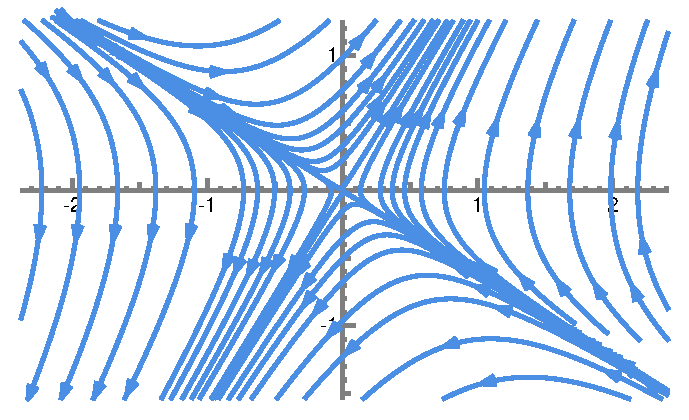
\includegraphics[width=0.75\textwidth]{sistemi_sella.pdf}
  \caption[1a]{sella (instabile)}
 \end{subfigure}
 \begin{subfigure}{5cm}
  %\centering
  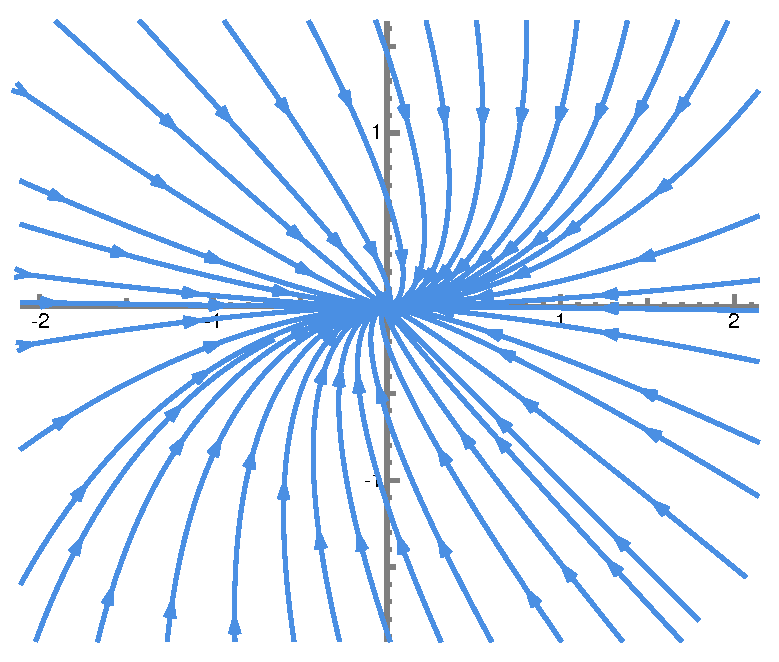
\includegraphics[width=0.75\textwidth]{sistemi_nodo.pdf}
  \caption{nodo stabile}
 \end{subfigure}
 \begin{subfigure}{5cm}
 \centering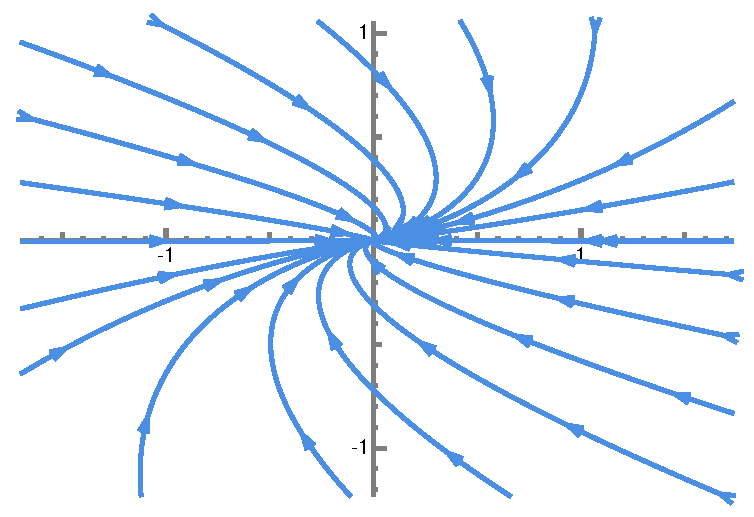
\includegraphics[width=0.75\textwidth]{sistemi_nodo_improprio.pdf}
  \caption{nodo improprio stabile}
 \end{subfigure}
 \begin{subfigure}{5cm}
  \centering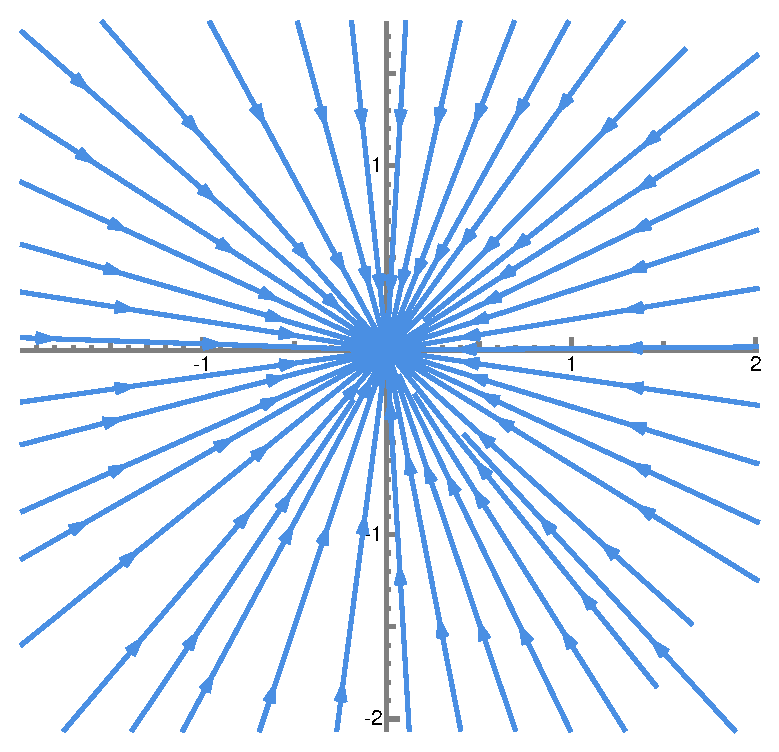
\includegraphics[width=0.75\textwidth]{sistemi_stella.pdf}
  \caption{stella stabile}
 \end{subfigure}
 \begin{subfigure}{5cm}
  \centering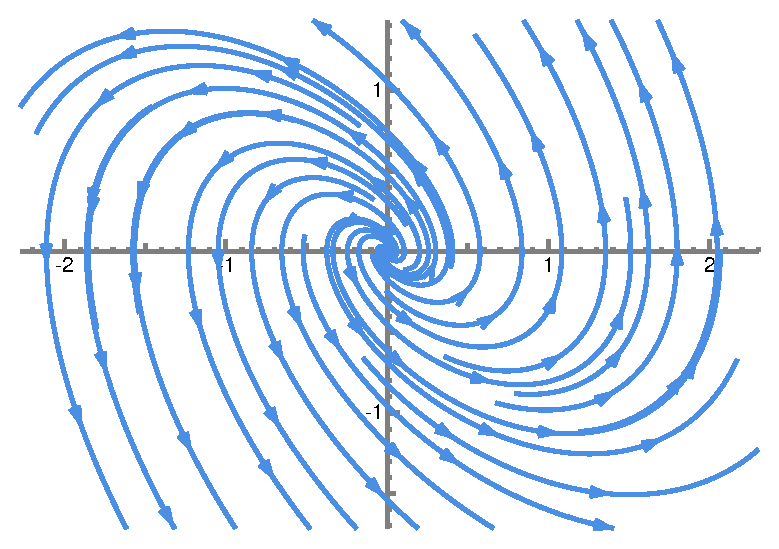
\includegraphics[width=0.75\textwidth]{sistemi_fuoco.pdf}
  \caption{fuoco stabile}
 \end{subfigure}
 \begin{subfigure}{5cm}
  \centering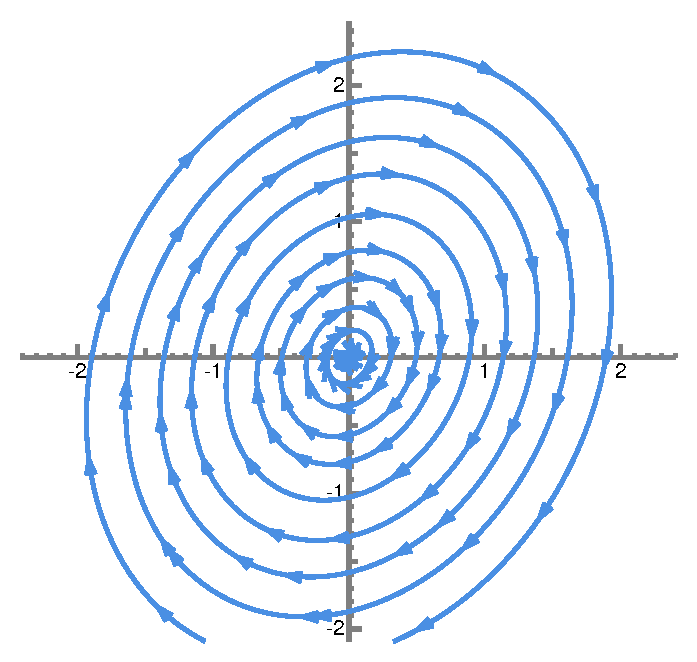
\includegraphics[width=0.75\textwidth]{sistemi_centro.pdf}
  \caption{centro (stabile)}
 \end{subfigure}
 \caption{\\%
 \usebox{\qrsistemisella} \usebox{\qrsisteminodo}\\
 \usebox{\qrsisteminodoimproprio} \usebox{\qrsistemistella}\\
 \usebox{\qrsistemifuoco} \usebox{\qrsistemicentro}
 }
\end{figure}

Se i segni di $\lambda$ e $\mu$ sono opposti,
si ottiene una configurazione chiamata
\emph{sella}%
\mymargin{sella}\index{sella} (si veda figura).
Lungo l'autovettore con autovalore negativo
ci sarà convergenza verso l'origine, ma questa
convergenza è instabile in quanto ogni altra
curva tenderà invece a essere deviata
e a tendere asintoticamente verso la direzione
dell'autovettore con autovalore positivo.

Se $\lambda$ e $\mu$ sono entrambi negativi si
ha un \emph{nodo stabile}%
\mymargin{nodo stabile}\index{nodo!stabile} in cui tutte le
curve convergono verso l'origine (soluzione
attrattiva). Se invece $\lambda$ e $\mu$
sono entrambi positivi le curve
saranno percorse in senso inverso e saranno
uscenti dall'origine: si avrà allora
un \emph{nodo instabile}%
\mymargin{nodo instabile}\index{nodo!instabile}.

Se gli autovalori sono coincidenti $\lambda=\mu$
e se la matrice è diagonalizzabile allora
la matrice è diagonale, tutti i vettori sono
autovettori quindi in ogni direzione c'è
una traiettoria rettilinea.
La configurazione si
chiama \emph{stella}%
\mymargin{stella}\index{stella} (stabile o instabile a seconda
del segno negativo o positivo).

Se gli autovalori sono coincidenti $\lambda = \mu$ e la matrice
non è diagonalizzabile consideriamo l'autovettore (unico)
$\vec u$ con $A \vec u = \lambda \vec u$
e prendiamo un qualunque vettore $\vec w$
indipendente da $\vec u$. Allora si avrà
\[
  A \vec w = \alpha \vec u + \beta \vec w.
\]
Certamente $\alpha \neq 0$ altrimenti $\vec w$
sarebbe un autovettore e la matrice sarebbe diagonalizzabile.
Consideriamo allora $\vec v = \vec w / \alpha$
cosicché si ha $A \vec v = \vec u + \frac{\beta}{\alpha} \vec w$.
Nella base $\vec u, \vec v$ la matrice $A$ diventa
triangolare, e sulla diagonale troviamo i valori $\lambda$
e $\frac{\beta}{\alpha}$.
Ma allora $\frac{\beta}{\alpha} = \lambda$ in quanto sulla diagonale
abbiamo solo gli autovalori. Dunque se $X,Y$ sono le coordinate nel
sistema $\vec u, \vec v$, il sistema di equazioni diventa:
\[
\begin{cases}
X' = \lambda X + Y \\
Y' = \lambda Y.
\end{cases}
\]
Dalla seconda equazione si ottiene quindi $Y = a e^{\lambda t}$
con $a\in \RR$ costante arbitraria
e sostituendo nella prima si ottiene l'equazione
\[
  X' - \lambda X = a e^{\lambda t}
\]
che può essere risolta trovando una seconda costante arbitraria $b\in \RR$ e
\[
  X = (at+b) e^{\lambda t}.
\]
Se $a=0$ una traiettoria con $Y=0$ cioè nella direzione dell'unico autovettore.
Se $\lambda <0$ tale traiettoria sarà convergente a $0$ altrimenti sarà divergente.
Se $a\neq 0$ possiamo eliminare $t$ ponendo:
\[
  t = \frac 1 \lambda \ln \frac{Y}{a}
\]
e quindi
\[
  X = \enclose{\frac{a}{\lambda} \ln \frac{Y}{a}+ b} \frac{Y}{a}
  =  \frac{Y}{\lambda}\ln \frac{Y}{a}+ \frac{b}{a}Y.
\]
Studiando il grafico di questa funzione si ottengono qualitativamente
le curve disegnate in figura: la configurazione si chiama \emph{nodo improprio}%
\mymargin{nodo improprio}\index{nodo improprio}.
Come per i nodi le traiettorie convergono all'origine se $\lambda < 0$ e
divergono se $\lambda >0$.

Proviamo a trattare il caso, più interessante,
degli autovalori complessi. Se la matrice è a coefficienti
reali gli autovalori, quando
non reali, saranno certamente complessi coniugati:
\[
  \lambda = \alpha - i \beta,
  \qquad
  \mu = \alpha + i \beta
\]
con $\alpha,\beta\in \RR$, $\beta\neq 0$.

Sia $\vec v + i \vec w$ un autovettore complesso relativo
all'autovalore $\alpha - i \beta$.
Allora si ha
\[
 A\vec v + i A \vec w
 = A(\vec v + i \vec w)
 = (\alpha - i \beta)(\vec v + i \vec w)
 = \alpha \vec v + \beta \vec w +i(-\beta \vec v + \alpha \vec w).
\]
Uguagliando parte reale e parte immaginaria si trova
\[
  A \vec v = \alpha \vec v + \beta \vec w,
  \qquad
  A \vec w = -\beta \vec v + \alpha \vec w.
\]
A questo punto non è difficile verificare che $\vec v - i \vec w$
è un autovettore relativo all'autovalore coniugato $\alpha + i\beta$.
Visto che $\vec v\pm i\vec w$ sono due autovettori con autovalori
distinti sicuramente sono vettori indipendenti.
Dunque anche $\vec v$ e $\vec w$
(che si ottengono come multipli di somma e differenza)
sono vettori indipendenti
(stavolta reali).
Se $X,Y$ sono le coordinate nella base $\vec v$, $\vec w$, l'equazione
differenziale diventa:
\[
\begin{cases}
 X' = \alpha X - \beta Y \\
 Y' = \beta X + \alpha Y.
\end{cases}
\]
Si ha allora%
\mynote{Si potrebbe osservare che la matrice
$\begin{pmatrix}\alpha&-\beta\\ \beta & \alpha\end{pmatrix}$
è la matrice che rappresenta la moltiplicazione
complessa per il numero $\alpha + i\beta$. Dunque chiamando $Z=X+iY$
il sistema si potrebbe scrivere nella forma $Z'=(\alpha +i\beta)Z$
e si potrebbe quindi osservare immediatamente
che la soluzione deve essere della forma $Z = c e^{(\alpha+i\beta)t}$
con $c$ costante complessa. Ponendo poi $c=\rho e^{i\theta}$
si ottiene il risultato.}
\[
 X'' = \alpha X' - \beta Y'
 = \alpha X' - \beta (\beta X + \alpha Y)
\]
da cui, usando $\beta Y = \alpha X - X'$ possiamo eliminare la variabile $Y$
e ottenere una equazione del secondo ordine in $X$:
\[
 X'' = \alpha X' - \beta^2 X - \alpha (\alpha X - X')
  = 2 \alpha X' - (\alpha^2+\beta^2) X
\]
ovvero
\[
 X'' - 2 \alpha X' + (\alpha^2 + \beta^2) X = 0.
\]
Risolvendo questa equazione del secondo ordine ci si accorge
che le radici del polinomio caratteristico sono proprio $\alpha \pm i \beta$
e quindi le soluzioni si scrivono nella forma
\[
X = e^{\alpha t}(a \cos \beta t + b \sin \beta t)
\]
da cui
\begin{align*}
\beta Y
&= \alpha X - X'\\
& = \alpha e^{\alpha t}(a \cos \beta t + b \sin \beta t) \\
&\quad - \alpha e^{\alpha t}(a\cos \beta t + b \sin \beta t)
  - e^{\alpha t}(-\beta a \sin \beta t + b \beta \cos \beta t) \\
 &= \beta e^{\alpha t}(a\sin \beta t - b \cos \beta t).
\end{align*}
Dunque, ponendo $\rho=\sqrt{a^2+b^2}$ e scegliendo $\theta$
tale che $\cos \theta = \frac a \rho$ e $\sin \theta = - \frac b \rho$,
si ha
\[
  \begin{cases}
   X = \rho e^{\alpha t} \cos(\beta t + \theta),\\
   Y = \rho e^{\alpha t} \sin(\beta t + \theta).
  \end{cases}
\]
Se $\alpha \neq 0$ le traiettorie corrispondenti formano delle spirali
ellittiche che si avvitano nella direzione che porta il vettore $\vec v$ verso
il vettore $\vec w$. Se $\alpha < 0$ le spirali convergono verso l'origine del
sistema: avremo un \emph{fuoco stabile}%
\mymargin{fuoco stabile}\index{fuoco stabile}. Se $\alpha >0$ le orbite
divergono chiameremo la configurazione un \emph{fuoco instabile}%
\mymargin{fuoco instabile}\index{fuoco instabile}.
Se $\alpha = 0$ le traiettorie sono delle ellissi concentriche,
le soluzioni sono quindi periodiche e la configurazione
si chiama \emph{centro}%
\mymargin{centro}\index{centro}.

Se almeno uno dei due autovalori è nullo il comportamento del sistema è degenere,
si hanno delle soluzioni banali che non andremo a investigare.

\subsection{matrice esponenziale}

Per risolvere, in astratto, il sistema $n\times n$ del primo ordine, 
lineare omogeneo a coefficienti costanti
\[
  \vec u' = A \vec u
\]
introduciamo le seguenti nozioni.

Sia $A$ una matrice quadrata $n\times n$. Definiamo la norma (norma
operatoriale) di $A$ come segue:
\[
  \Abs{ A } = \sup_{\abs{\vec v} \le 1} \abs{A\vec v}
\]
dove $\abs{ \vec v} = \sqrt{v_1^2+ \dots + v_n^2}$ è l'usuale norma del
vettore $\vec v\in \RR^n$.
Osserviamo che $\vec v\mapsto A\vec v$ è una funzione
continua e che $\ENCLOSE{\vec v\colon \abs{ \vec v} \le 1}$ è un insieme
compatto, dunque il $\sup$ nella definizione è in realtà un $\max$.

Per le proprietà del $\sup$ si ha:
\[
  \abs{A\vec v} \le \Abs{ A }\, \abs{ v }
\qquad\text{e}\qquad
  \Abs{ A B } \le \Abs{ A } \, \Abs{ B }.
\]
Dunque possiamo affermare il valore assoluto di ogni elemento di una
matrice si stima con la norma della matrice: $\abs{ A_{ij}} \le
\Abs{ A }$, infatti:
\[
  \abs{ A_{ij} } = \abs{ (A \vec e_j)_i} \le \abs{ A e_j}
  \le \Abs{ A }
\]
(dove $\vec e_j$ è il $j$-esimo vettore della base canonica di $\RR^n$).

Se $A_k$ è una successione di matrici, diremo che $A_k\to A$ se ogni
elemento della matrice $A_k$ converge al corrispondente elemento della
matrice $A$: $(A_k)_{ij} \to A_{ij}$. Questo corrisponde a considerare
la matrice $n\times n$ come un vettore dello spazio $\RR^{(n^2)}$.

Se $A(t)$ è una funzione a valori matrici (ovvero una matrice i cui
elementi sono funzioni di $t$), si potrà farne la derivata
come si fa per le funzioni vettoriali: $(A'(t))_{ij} = (A_{ij}(t))'$
cioè componente per componente. Le usuali regole per le derivate
valgono anche per le matrici, in particolare non è difficile
verificare (si espliciti la definizione del prodotto di matrici) che
\[
 (A(t)B(t))' = A'(t) B(t) + A(t) B'(t)
\]
dove, puntualizziamo, è importante mantenere i prodotti nell'ordine
giusto, in quanto il prodotto di matrici può non essere commutativo.

Se $A$ è una matrice quadrata, si definisce la matrice potenza $A^k$
per ogni $k$ naturale, mediante le proprietà
\[
  A^0 = I, \qquad A^{k+1} = A^kA.
\]
(se $A$ è invertibile si possono definire anche le potenze negative
$A^{-k}=(A^{-1})^k = (A^k)^{-1}$).

Definiamo allora la matrice esponenziale di $A$:
\[
  e^A = \sum_{k=0}^{+\infty} \frac{A^k}{k!}.
\]
Per dare significato a questa definizione dobbiamo verificare che la
serie appena scritta sia convergente. Cioè dobbiamo verificare che per
ogni coppia di indici $ij$ sia convergente la serie numerica:
\[
 \sum_{k=0}^{+\infty} \frac{(A^k)_{ij}}{k!}.
\]
Per quanto detto prima sappiamo che
$\abs{(A^k)_{ij}} \le \Abs{A^k} \le \Abs{A}^k$.
Dunque la serie in questione è
assolutamente convergente in quanto il suo valore assoluto si stima
con la serie
\[
 \sum_{k=0}^{+\infty} \frac{\Abs{ A}^k}{k!} = e^{\Abs{ A}}
\]
che è convergente. La definizione della matrice $e^A$ è dunque
ben posta e si ha
\[
 \Abs{ e^A} \le e^{\Abs{ A }}.
\]

\begin{theorem}[proprietà dell'esponenziale matrice]
Siano $A$ e $B$ matrici quadrate $n\times n$ e $t$ uno scalare.
Valgono le seguenti proprietà:
\begin{enumerate}
\item $e^0 = I$ (dove $0$ è la matrice nulla $n\times n$ ed $I$ è la
  matrice identità con le stesse dimensioni);
\item se $AB=BA$ allora $e^A B = B e^A$;
\item $(e^{tA})' = A e^{tA}$;
\item $e^{-A} = (e^A)^{-1}$ (in particolare la matrice esponenziale è
  sempre invertibile);
\item se $\vec u(t)$ è una funzione a valori in $\RR^n$ che soddisfa
  l'equazione differenziale $\vec u'(t) = A\vec u(t)$ allora
  $\vec u(t) = e^{tA} \vec u(0)$;
\item se $AB=BA$ allora $e^{A+B} = e^A e^B$;
\item se $A$ è invertibile allora $e^{ABA^{-1}} = Ae^BA^{-1}$;
\item se $A$ è la matrice diagonale $A = \diag(\lambda_1, \dots, \lambda_n)$,
allora $e^A$
 è pure una matrice diagonale con $e^A = \diag(e^{\lambda_1},\dots, e^{\lambda_n})$;
\item se $A$ è una matrice triangolare con la diagonale nulla (cioè
  $A_{ij}=0$ se $i\ge j$) allora $e^A = \sum_{k=0}^n \frac{A^k}{k!}$
  (basta sommare i primi $n+1$ termini);
\item se $B$ è una matrice triangolare (cioè $B_{ij}=0$ se $i > j$)
  allora $B = D + A$ con $D$ matrice diagonale e $A$ matrice
  triangolare con la diagonale nulla e quindi $e^B = e^De^A$ si può
  calcolare riconducendosi ai punti precedenti.
\end{enumerate}
\begin{proof}
1. Per quanto riguarda $e^0$ osserviamo che per definizione $0^0=I$
mentre $0^k=0$ se $k>0$. Dunque direttamente dalla definizione si
ottiene $e^0=I$.

2. Se $AB=BA$ osserviamo che si ha anche $A^k B=B A^k$ (la matrice $B$
commuta con ogni fattore del prodotto $A^k$). Dunque:
\[
 \sum_{k=0}^N \frac{A^k}{k!} B = B \sum_{k=0}^N \frac{A^k}{k!}
\]
e passando al limite $N\to \infty$ si ottiene $e^A B = B e^A$.

3. Per calcolare la derivata di $e^{tA}$ vogliamo dimostrare che la serie
che definisce $e^{tA}$ converge totalmente quando $t$ varia in un
qualunque intervallo limitato. Poniamo allora $t\in [-M,M]$. Si ha:
\[
  \sup_{t\in[-M,M]}\frac{\Abs{ (tA)^k}}{k!}
  = \sup_{t\in[-M,M]}\frac{\abs{ t}^k \Abs{ A^k}}{k!}
  \le \frac{M^k\Abs{ A}^k}{k!}
\]
la cui serie è convergente qualunque sia $M\in \RR$. Dunque la serie
che definisce $e^{tA}$ è una serie di funzioni continue e derivabili
che converge totalmente su ogni intervallo limitato. Possiamo quindi
derivare la serie termine a termine:
\[
(e^{tA})' = \sum_{k=0}^\infty \frac{((tA)^k)'}{k!}
 = \sum_{k=1}^\infty \frac{kt^{k-1} A^k}{k!}
 = A \sum_{k=1}^\infty \frac{t^{k-1}A^{k-1}}{(k-1)!}
 = A e^{tA}.
\]

4. Dimostriamo ora che $U(t) = e^{tA}e^{-tA}=I$ per ogni $t$. Si ha:
\[
 U'(t) = A e^{tA}e^{-tA} + e^{tA}(-A)e^{-tA}
       = A e^{tA}e^{-tA} - A e^{tA}e^{-tA} = 0
\]
($Ae^{tA} = e^{tA}A$ in quanto $A$ e $tA$ commutano).
Dunque $U'(t)=0$ cioè $U(t)$ è costante ovvero $U(t)=U(0)$. Ma $U(0)=I$
in quanto $e^0=I$ e quindi $U(t)=I$ per ogni $t$.

5. Prendiamo l'equazione $\vec u' = A\vec u$, moltiplicando a sinistra per
$e^{-tA}$ l'equazione diventa
$e^{-tA} \vec u' - e^{-tA} A \vec u=0$ cioè $(e^{-tA} \vec u)' = 0$. Questo significa
che la funzione $e^{-tA}\vec u = c$ costante e moltiplicando a sinistra per
$e^{tA}$ si ottiene dunque $\vec u = e^{tA}c$ come volevasi dimostrare.

6. Per dimostrare la proprietà $e^{A+B}=e^A e^B$ consideriamo la quantità
$U(t) = e^{-t(A+B)} e^{tA} e^{tB}$. Se dimostriamo che $U$ è costante,
visto che $\vec u(0)=I$ si avrà anche $U(1)=I$ che è equivalente a quanto
vogliamo dimostrare. Dunque verifichiamo che la derivata è nulla,
sfruttando l'ipotesi $AB=BA$ che ci permette di far commutare i prodotti:
\begin{align*}
U'(t) & = -(A+B)e^{-t(A+B)} e^{tA} e^{tB} + e^{-t(A+B)}Ae^{tA}e^{tB} +
e^{-t(A+B)}e^{tA} B e^{tB} \\
& = [-(A+B) + A + B] U(t) = 0.
\end{align*}

7. Se $A$ è invertibile allora $(ABA^{-1})^k = ABA^{-1}ABA\dots ABA^{-1}
= AB^k A^{-1}$. Dunque nelle somme parziali della serie che definisce l'esponenziale
$e^{ABA^{-1}}$ si può raccogliere $A$ a sinistra e $A^{-1}$ a destra e
al centro rimane la serie che definisce $e^B$.

8. Se la matrice $A$ è diagonale con $A_{ii}=\lambda_i$ allora $A^k$
risulta essere una matrice diagonale con $(A^k)_{ii} =
\lambda_i^k$. Dunque nella definizione di esponenziale $e^A$ i termini
della serie sono tutte matrici diagonali, e sulla diagonale compare la
serie che definisce l'esponenziale $e^{\lambda_i}$.

9. Se $A$ è una matrice triangolare con $A_{ij}=0$ quando $i\ge j$, si
osserva che $A^2$ avrà degli zeri anche sopra la diagonale:
$(A^2)_{ij}=0$ quando $i+1\ge j$ (si applichi la definizione di
prodotto, riga per colonna). Nelle moltiplicazioni successive $A^3,
A^4,\dots$ si aggiungerà sempre una diagonale di zeri finché la matrice non
si annulla completamente $A^n=0$. Dunque la serie che definisce $e^A$
contiene solo un numero finito di termini (i primi $n+1$) e può essere
calcolata esplicitamente.

10. L'ultima proprietà è una osservazione che non richiede dimostrazione.
\end{proof}
\end{theorem}


\section{modelli biologici di crescita}
\index{modello!biologico}%

\subsection{modello di Malthus}
\index{modello!di Malthus}%
\index{Malthus!modello di}%
\index{esponenziale!modello di Malthus}%

Il più semplice modello di crescita di una popolazione è quello 
in cui si suppone che la popolazione abbia nutrimento e spazio sufficiente 
per una crescita indeterminata.
In questo modello la funzione $u(x)$ rappresenta la quantità di individui 
al tempo $x$ e si suppone che la velocità di crescita della popolazione $u'(x)$ 
sia proporzionale al numero di individui:
\[
  u'(x) = A u(x).  
\]
La soluzione di questa semplice equazione lineare (esercizio~\ref{ex:58230978})
è $u(x) = u_0\cdot  e^{A x}$ dove $u_0=u(0)$ è la popolazione al tempo 
iniziale $x=0$.
Significa che se $A>1$ la popolazione cresce indefinitamente tendendo 
a $+\infty$ per $x\to +\infty$ con velocità esponenziale.
Se $A<1$ invece la popolazione tende a zero (cioè si estingue)
sempre con velocità esponenziale.

\subsection{equazione logistica}
\index{equazione!logistica}%
\index{logistica!equazione differenziale}%
\index{crescita!logistica}%

Per rendere il modello di Malthus più realistico bisogna tenere conto 
del fatto che gli individui condividono uno spazio comune e che 
la presenza di molti individui nello stesso spazio diminuisce le risorse 
e quindi contribuisce in negativo alla crescita della popolazione. 
Supponiamo quindi che l'effetto negativo su una unità di popolazione 
sia proporzionale alla popolazione totale: $-Bu$ mentre l'aumento 
Malthusiano è sempre dato dal coefficiente $A$ per unità di popolazione. 
Si avrà quindi 
\[
  u'(x)  = (A-Bu(x))\cdot u(x)
\]
Questa è una equazione a variabili separabili. 
Le funzioni $u(x) = 0$ e $u(x) = \frac{A}{B}$ sono soluzioni 
stazionarie (ovvero costanti). 
La prima rappresenta una popolazione vuota, che quindi non potrà 
mai crescere. 
La soluzione $u=\frac{A}{B}$ rappresenta una popolazione 
in perfetto equilibrio.
Per semplificare le notazioni possiamo fare il cambio di variabile 
$v(x) = \frac{B}{A}\cdot u(x/A)$ che ci porta alla equazione 
equivalente $v'=(1-v)\cdot v$. 
Possiamo quindi supporre che sia $A=1$ e $B=1$ e ritornare 
alla variabile $u$:
\begin{equation}\label{eq:ode_logistica}
  u' = (1-u) u.  
\end{equation}

\newsavebox{\qrOdeLogistica}\sbox{\qrOdeLogistica}{%
\myqrshortdoclink{ode_logistica}{Le soluzioni dell'equazione logistica~\eqref{eq:ode_logistica}}}
\begin{figure}
  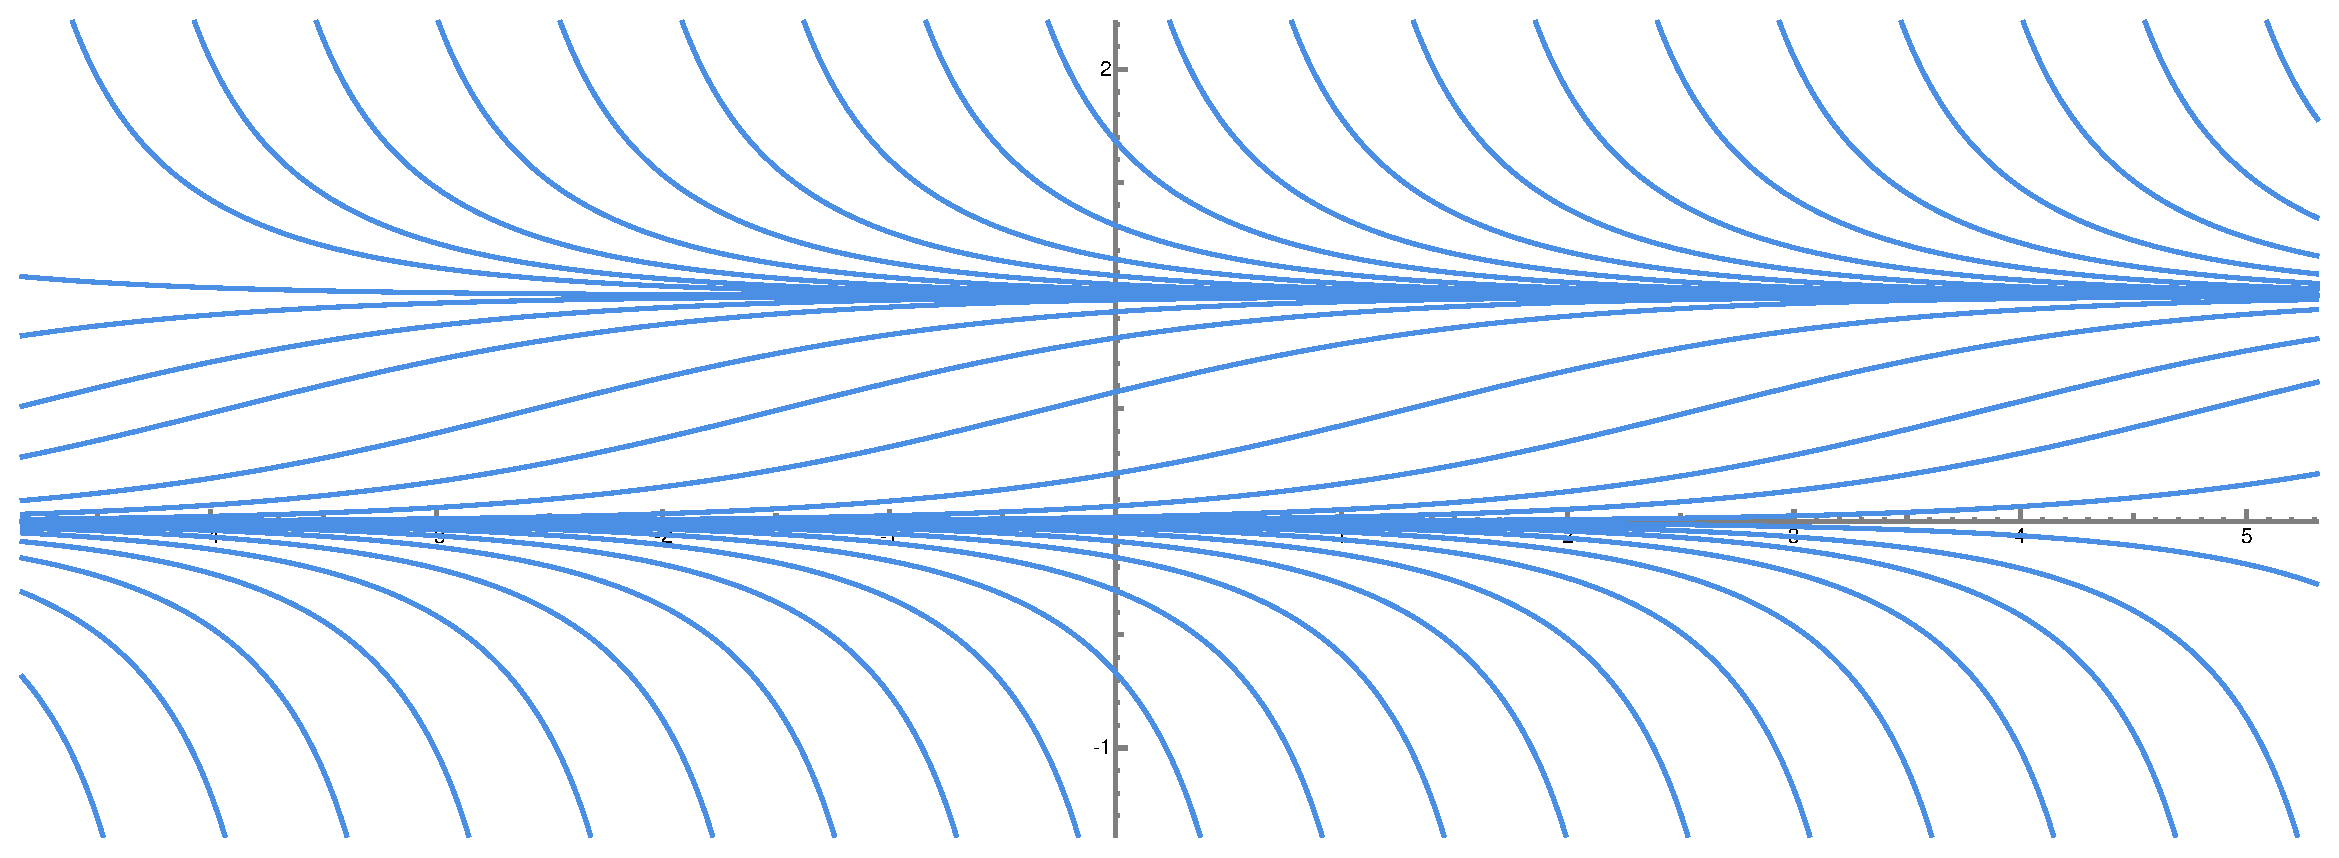
\includegraphics[width=\textwidth]{ode_logistica.pdf}
  \caption{
Le soluzioni dell'equazione logistica~\eqref{eq:ode_logistica}.
\ifwidemargin\\\\\fi%
\usebox{\qrOdeLogistica}}
\label{fig:ode_logistica}
\end{figure}

Avendo identificato le soluzioni stazionarie $u=0$ e $u=1$ possiamo separare le variabili
e integrare:
\[
 \int \frac{u'}{(1-u)u}\, dx = x - x_0.
\]
L'integrale si decompone con il metodo dei fratti semplici:
\[
  \int \frac{u'}{(1-u)u}\, dx
  = \int \frac{1}{(1-u)u}\, du 
  = \int \Enclose{\frac{1}{u} + \frac{1}{1-u}}\, du 
  = \ln \abs{u} - \ln\abs{1-u}
  = \ln \abs{\frac{u}{1-u}}.
\]
Dunque da 
\[
\abs{\frac{u}{1-u}} = e^{x-x_0}  
\]
si ottiene, con qualche passaggio algebrico,
\[
    u(x) = 1 - \frac{1}{1\pm e^{x-x_0}}.
\]
Il grafico di queste funzioni è rappresentato in figura~\ref{fig:ode_logistica}.
Nel capitolo~\ref{sec:studio_qualitativo_edo}
vedremo come risulta molto semplice ottenere l'andamento qualitativo dei grafici 
delle soluzioni di questa equazione senza doverne determinare esplicitamente 
le soluzioni.

\subsection{il modello di Volterra-Lotka}
\index{modello!di Volterra-Lotka}%
\index{Volterra!modello preda-predatore}%
\index{Lotka!modella preda-predatore}%
\index{preda/predatore}%

Il modello preda/predatore di Volterra-Lotka è il primo esempio 
di modello matematico applicato alla biologia.
\index{Volterra Vito}%
Il matematico italiano Vito Volterra si era interessato al problema 
di capire, tramite un modello matematico, il fenomeno apparentemente 
paradossale per cui il calo delle attività di pesca 
durante la prima guerra mondiale ha causato alla ripresa della pesca 
una diminuzione della 
quantità di pesce commestibile e un contemporaneo relativo aumento delle 
specie predatorie come gli squali.

Nel modello preda/predatore ideato da Volterra denotiamo con $u(x)$ 
la numerosità della popolazione di prede e con $v(x)$ la numerosità 
dei predatori al variare del tempo $x$.
Il modello è quindi rappresentato da un sistema di equazioni
non lineari del primo ordine:
\begin{equation}\label{eq:preda_predatore}
  \begin{cases}
    u' = A u - B u v \\
    v' = C u v - D v
  \end{cases}
\end{equation}
con $A,B,C,D$ costanti reali positive.
Il fattore di crescita delle prede è dettata da una legge di Malthus
$A u$ che rappresenta l'autosufficienza delle prede (si suppone 
abbiano sufficiente nutrimento per crescere indefinitamente).
L'addendo $-B u v$ rappresenta l'uccisione delle prede 
da parte dei predatori: è un termine proporzionale sia alla popolazione 
$u$ delle prede che alla popolazione $v$ dei predatori (come se ogni preda 
avesse un probabilità proporzionale a $v$ di incontrare un predatore).
Il termine $C u v$ rappresenta la corrispondente 
crescita dei predatori grazie al nutrimento dato dalle prede.
Viceversa i predatori non possono sostentarsi autonomamente e quindi 
il termine $-D v$ rappresenta l'estinguersi naturale dei predatori 
in assenza di nutrimento.

Alcune soluzioni del sistema~\eqref{eq:preda_predatore} possono essere 
trovate esplicitamente. 
Ad esempio se $v=0$ ci riconduciamo all'equazione di Malthus per $u$ 
e troviamo $u(x) = k e^{Ax}$: la preda cresce esponenzialmente in 
assenza di predatori.
Analogamente se $u=0$ si trova $v(x) = k e^{-Dx}$: i predatori 
si estinguono con velocità esponenziale in assenza di prede.


Possiamo inoltre trovare soluzioni stazionarie (cioè costanti) ponendo 
$u'=0$ e $v'=0$. Riscriviamo il sistema nella forma:
\begin{equation}\label{eq:preda_predatore_2}
  \begin{cases}
    u' = u \cdot (A - B v) \\
    v' = v \cdot (C u - D).
  \end{cases}
\end{equation}
e osserviamo quindi che per annullare contemporaneamente $u'$ e $v'$ 
si deve avere o $u=0$ e $v=0$ (soluzione in cui non ci sono né prede né predatori)
oppure si può avere $u=\frac D C$ e $v=\frac A B$ che è un punto di equilibrio
non banale tra le due specie.

Possiamo ottenere informazioni piuttosto precise 
se riusciamo ad identificare un integrale 
del sistema ovvero una funzione $H(u,v)$ che rimane costante sulle soluzioni: 
$\frac {d}{dx} H(u(x),v(x)) = 0$. 
Facendo il rapporto tra le due equazioni del sistema~\eqref{eq:preda_predatore_2}
si ottiene 
\[
  \frac{v'}{u'} 
  = \frac{v \cdot (C u - D)}{u \cdot (A - B v)}
\]
separando le variabili
\[
  \frac{A - B v}{v} v' = \frac{C u - D}{u} u'
\]
integrando in $dx$
\[
  \int \frac{A - B v}{v} v'\, dx  = \int \frac{C u - D}{u} u'  \, dx
\]
facendo i cambi di variabile $u=u(x)$, $v=v(x)$, $du = u'\, dx$, $dv=v'\, dx$
ed eseguendo le divisioni:
\[     
  \int \Enclose{\frac A v - B}\, dv = \int \Enclose{C  - \frac D u}\, du
\]
da cui, per una qualche costante $k$:
\[
  A \ln v - B v = C u - D\ln u + k.
\]
Significa che la funzione 
\[
  H(u,v) = B v + C u - A \ln v - D \ln u
\]
è costante lungo le curve $(u(x),v(x))$.
Dunque le traiettorie del sistema 
con $u>0$ e $v>0$ sono limitate, perché se 
$u$ oppure $v$ andassero all'infinito 
i termini $Bv-A\ln v$ o $Cu - D \ln u$ andrebbero 
anch'essi all'infinito e la funzione $H$ non 
potrebbe essere costante.

\newsavebox{\qrEdoVolterra}\sbox{\qrEdoVolterra}{%
  \myqrshortdoclink{edo_volterra}{Orbite del sistema preda/predatore~\ref{eq:preda_predatore}}}
\begin{figure}
  \begin{center}
    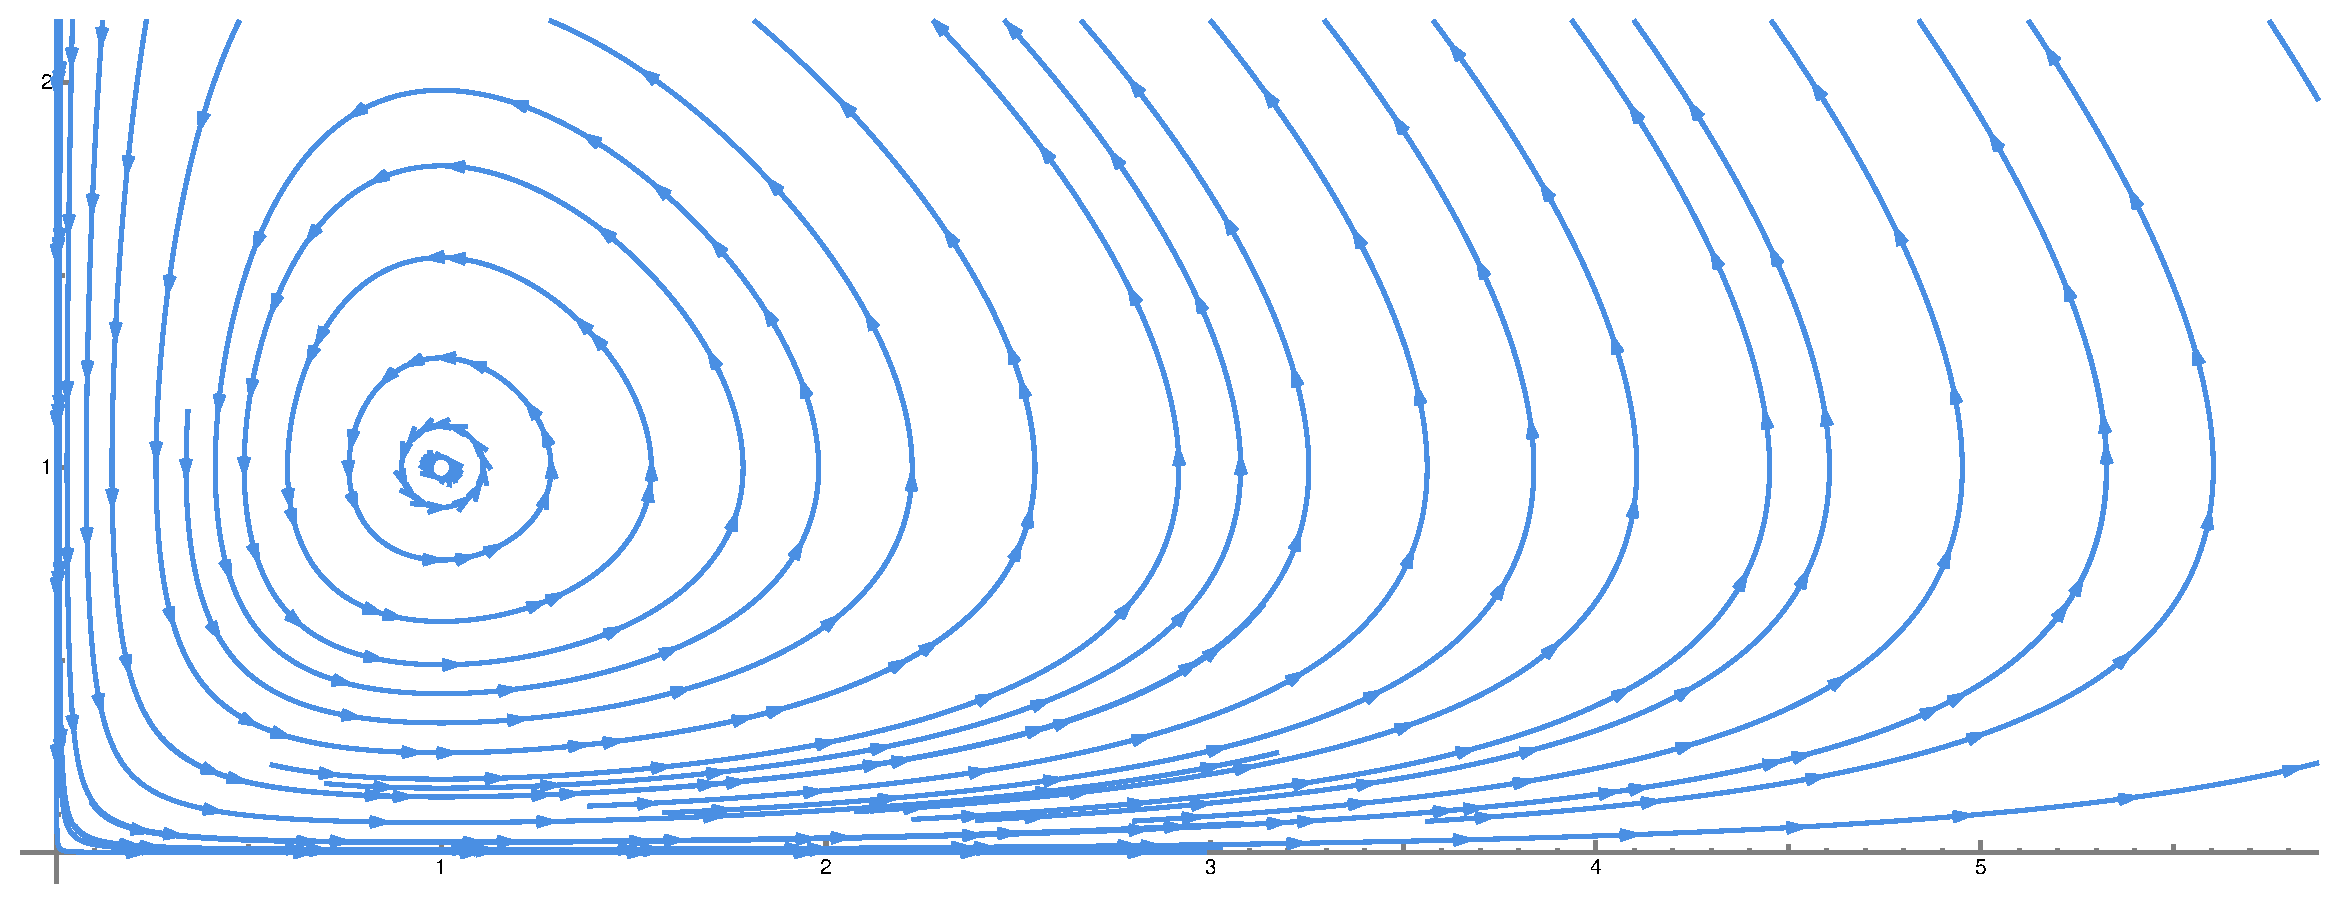
\includegraphics[width=\textwidth]{ode_volterra.pdf}
  \end{center}
  \caption{
  Le orbite del sistema preda/predatore~\eqref{eq:preda_predatore} 
  con la scelta dei parametri $A=B=C=D=1$.
  \ifwidemargin\\\\\fi%
  \usebox{\qrEdoVolterra}}
  \label{fig:ode_volterra}
\end{figure}

Consideriamo ora una soluzione $u(x),v(x)$ che al tempo $x_0$ 
si trova sul segmento $u=\frac DC$ e $v\in \openinterval{0}{\frac A B}$
(si faccia riferimento alla figura~\ref{fig:ode_volterra} dove abbiamo 
posto $\frac AB=1$ e $\frac DC=1$).
Siccome $v<\frac A B$ si ha $u'>0$ e quindi la curva si sposta verso destra.
Non appena $u>\frac DC$ si ha anche $v'>0$ e quindi la curva si sposta 
anche verso l'alto. Siccome $u$ non può tendere all'infinito 
prima o poi la soluzione deve raggiungere la retta $v=\frac AB$ 
dove la derivata di $u$ si annulla e la curva si sposta quindi 
in direzione verticale. Diventa quindi $v>\frac AB$ dove $u'<0$.
La coordinata $u$ dunque cala e siccome $v$ non può tendere all'infinito 
$u$ dovrà raggiungere il valore $\frac DC$ dove si ha $v'=0$.
Quindi si prosegue con $u<\frac DC$ dove $v'<0$.
Dunque ora sia $u$ che $v$ calano.
Devono però rimanere positivi sia perché la funzione $H$ tende all'infinito 
anche quando $u\to 0$ o $v\to 0$ sia perché gli assi $u=0$ e $v=0$ 
sono orbite delle soluzioni esplicite che abbiamo trovato inizialmente 
e per l'unicità delle soluzioni non è possibile che orbite diverse 
si incontrino in un punto.
Dunque ad un certo punto si avrà di nuovo $v= \frac AB$ e $u\in \openinterval{0}{\frac DC}$
e poi si avrà $v<\frac AB$ con $u'>0$ e $v'<0$.
La nostra curva dovrà quindi di nuovo raggiungere in un istante $x_1>x_0$ 
il segmento da cui 
eravamo partiti: $u=\frac DC$ e $v\in \openinterval{0}{\frac AB}$.
In tutto questo percorso $H$ è rimasta costante dunque si avrà 
$H(u(x_1),v(x_1))=H(u(x_2),v(x_2))$. 
Ma $u(x_1)=u(x_2) = \frac DC$ e posto $f(v) = H(D/C,v)$ si osserva che 
\begin{align*}
   f(v) = B v + D - A \ln v - D \ln \frac DC.
\end{align*}
studiando il segno della derivata $f'(v)=B-\frac{A}{v}$ si osserva che per $v<\frac AB$ 
la derivata è strettamente negativa dunque la funzione $f$ è strettamente 
decrescente nell'intervallo $v\in(0,D/C)$ dunque iniettiva.
Essendo $f(v(x_1)) = f(v(x_2))$ deduciamo quindi che $v(x_1)=v(x_2)$.
Significa che la curva si richiude e le soluzioni sono dunque 
periodiche di periodo $T=x_2-x_1$. 

Preso un qualunque punto del quadrante $u>0$, $v>0$ (escluso il punto
critico) la soluzione che parte
da quel punto seguirà un percorso che, in base alle considerazioni che abbiamo già 
fatto, è costretto prima o poi ad attraversare il segmento che abbiamo 
preso in considerazione e quindi è, in effetti, una di quelle che 
abbiamo già studiato.

Questo studio qualitativo descrive l'andamento delle soluzioni 
del sistema~\ref{eq:preda_predatore}: si cerchi di interpretare 
il significato biologico di quanto abbiamo dedotto. Metodi numerici 
(come quelli utilizzati per ottenere la figura~\ref{fig:ode_volterra})
ci permettono di ottenere informazioni quantitative con la precisione 
desiderata.

Possiamo ora anche rispondere alla domanda iniziale rivolta a Vito Volterra 
e cioè spiegare cosa succede in presenza dell'attività umana di pesca.
Il sistema studiato finora è quello che descrive l'andamento in assenza 
dell'attività di pesca (cioè quanto veniva osservato dai naturalisti alla fine della 
prima guerra mondiale). 
In presenza di pesca intensiva dobbiamo supporre che la quantità di pesce 
pescato è proporzionale, per ogni specie, alla numerosità della specie stessa.
Dunque dobbiamo sottrarre un termine $Eu$ dalla prima equazione e un termine 
corrispondente $Ev$ dalla seconda:
\begin{equation}
  \begin{cases}
    u' = A u - B u v - Eu = (A-E) u - B uv\\
    v' = C u v - D v - Ev = C uv - (D+E) v.
  \end{cases}
\end{equation}
Si osserva quindi che il sistema rimane dello stesso tipo solo che 
il coefficiente $A$ è diminuito diventando $A-E$ mentre il coefficiente 
$D$ è aumentato diventando $D+E$.
Dunque il punto di equilibrio $u=\frac DC$, $v=\frac AB$ si è spostato 
verso destra e verso il basso in quanto $D$ è aumentato e $A$ è diminuito.
Questo significa che in media l'attività di pesca favorisce un aumento 
delle prede e una diminuzione dei predatori. 
Viceversa la diminuzione dell'attività di pesca fa diminuire la quantità
di prede e aumentare quella dei predatori.


\section{studio qualitativo delle soluzioni}
\label{sec:studio_qualitativo_edo}

Non sempre è possibile determinare esplicitamente le soluzioni
di una equazione differenziale.
Ci proponiamo quindi di trovare dei metodi per
determinare alcune proprietà salienti delle soluzioni, senza
doverle determinare esplicitamente.
Considereremo unicamente equazioni del primo ordine in forma normale:
\begin{equation}\label{eqdiff}
	u'(x)= f(x,u(x))
\end{equation}
con $f\colon \Omega \subset \RR^2\to \RR$.

Ricordiamo che se $f$ soddisfa la condizione di Cauchy-Lipschitz
(definizione~\ref{def:cauchy_lipschitz}), in particolare
se $f$ è di classe $C^1$ allora i grafici delle soluzioni
massimali dell'equazione differenziale~\eqref{eqdiff}
\emph{fibrano} la regione $\Omega$ nel senso che per ogni punto di
$\Omega$ passa una unica soluzione massimale (teorema~\ref{th:cauchy_lipschitz}
di Cauchy-Lipschitz e proposizione~\ref{prop:separazione_soluzioni}).
Inoltre la proposizione~\ref{prop:edo_massimale} ci dice
che le soluzioni massimali escono da qualunque compatto contenuto in
$\Omega$ ovvero raggiungono sempre la frontiera di $\Omega$.

\begin{example}\label{ex:edo_4630b}
Sia $u$ la soluzione massimale del problema di Cauchy
\[
	\begin{cases}
		u' = \cos(u^2)\cdot \sin x, \\
		u(0) = 0.
	\end{cases}
\]
Mostrare che $u$
è definita su tutto $\RR$ (dunque la soluzione è globale).
Mostrare che $u$ è pari.
Mostrare che $u$ è periodica.
Mostrare che $u(x)\ge 0$ per ogni $x\in \RR$.
\end{example}
\newsavebox{\qredoquattro}\sbox{\qredoquattro}{%
\myqrshortdoclink{edo_4630b}{Studio qualitativo esempio \getrefnumber{ex:edo_4630b}}}
\begin{figure}
  \centering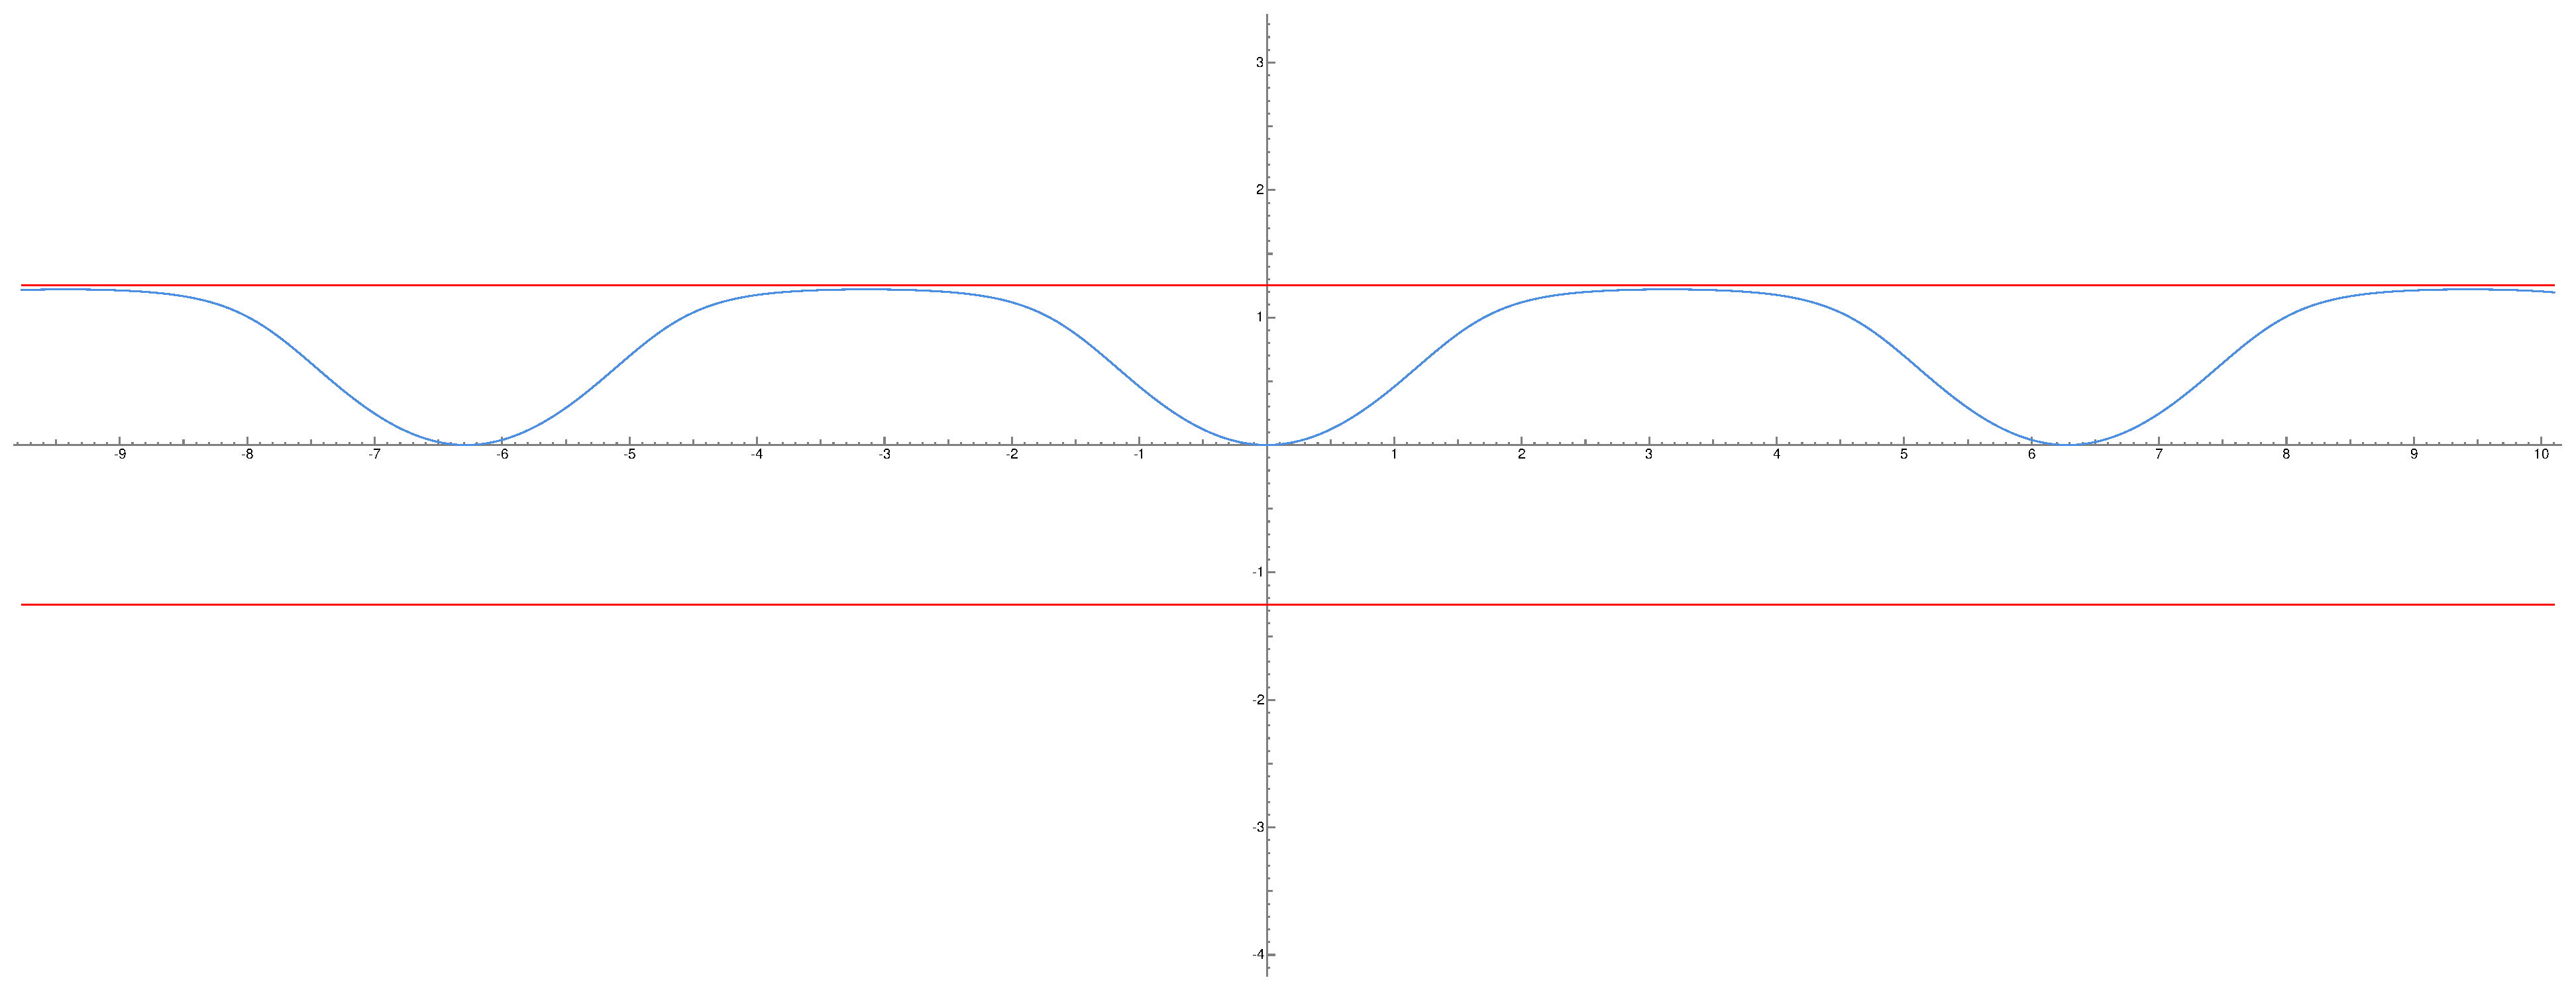
\includegraphics[width=\textwidth]{edo_4630b}
  \caption{Studio qualitativo dell'esempio~\ref{ex:edo_4630b}.
  \ifwidemargin\\\\\fi%
  \usebox{\qredoquattro}}
  \label{fig:edo_4630b}
\end{figure}
%
\begin{proof}[Svolgimento.]
In questo caso si ha $f(x,y)=\cos y^2\cdot \sin x$, che \`e una funzione
di classe $C^1$ su tutto $\Omega=\RR^2$.
Vale dunque il teorema di esistenza ed
unicità delle soluzioni.
Notiamo inoltre (per verifica diretta)
che posto $H=\sqrt{\frac \pi 2}$, le funzionie 
costanti $u_0(x)=-H$ e $u_1(x)=H$ sono
soluzioni dell'equazione differenziale (\ref{eqdiff})
in quanto $f\enclose{x,\pm H}=0$ per ogni $x\in \RR$
(soluzioni \emph{stazionarie}).
Per la proposizione~\ref{prop:separazione_soluzioni},
il grafico della soluzione $u(x)$
non può toccare i grafici delle due funzioni $u_0$ e $u_1$ e visto
che $u(0)=0$ e che $u$ è una funzione continua significa
che per ogni $x$ si ha $-H < u(x) < H$.
Consideriamo ora il compatto
$K_M=[-M,M] \times [-H,H]$.
Sappiamo che la soluzione
massimale $u(x)$ del problema di Cauchy preso in considerazione deve
uscire da ogni compatto $K_M$
(proposizione~\ref{prop:edo_massimale}).
Visto però che $u(x)\in (-H,H)$ significa che necessariamente
il grafico della soluzione massimale $u(x)$
raggiunge i due segmenti verticali
$x=-M$ e $x=M$ e dunque l'intervallo massimale di esistenza
contiene l'intervallo $[-M,M]$.
Siccome questo è vero per ogni $M$, l'intervallo massimale
di esistenza della soluzione è $I=\RR$ e dunque la soluzione
è globale.

Dimostriamo che $u$ è pari. Sia $v(x)=u(-x)$. 
Si ha 
\[ 
    v'(x) = -u'(-x) 
    = -\cos(u^2(-x))\cdot \sin(-x) 
    = \cos(v^2(x))\cdot \sin(x)
\]
da cui risulta che $v$ soddisfa la stessa equazione differenziale 
di cui $u$ è soluzione. 
Inoltre $v(0)=u(0)=0$ e quindi $u$ e $v$ sono soluzioni dello 
stesso problema di Cauchy. Per unicità della soluzione 
deve essere $u(x)=v(x)$ per ogni $x$ e quindi $u(-x)=u(x)$, come 
volevamo dimostrare.
  
Dimostriamo ora che $u$ è $2\pi$-periodica.
Sia $w(x)=u(x+2\pi)$. Si ha allora 
\[
  w'(x) = u'(x+2\pi) = \cos(u^2(x+2\pi))\cdot \sin(x+2\pi) 
  = \cos(w^2(x))\cdot \sin(x) 
\]
dunque, di nuovo, $w$ soddisfa la stessa equazione differenziale
di cui $w$ è soluzione. Si ha inoltre 
\[
  u(-2\pi) - w(-2\pi) = u(2\pi) - u(0) = w(0) - u(0).
\]
Questo significa che $u-v$ assume segno opposto nei punti 
$a=-2\pi$ e $b=0$ e quindi, per il teorema~\ref{th:valori_intermedi}
dei valori intermedi ci deve essere un punto in cui le due 
$u-v$ si annulla. In tale punto ho due soluzioni dello stesso 
problema di Cauchy e dunque, per l'unicità della soluzione, 
dobbiamo concludere che $u(x)=v(x)$ per ogni $x$.
Questo significa che $u$ è $2\pi$-periodica.

Visto che $\abs{u(x)}<H$ con $H^2=\pi 2$ si ha che $\cos(u^2(x))>0$ 
e quindi $u'(x)$ ha lo stesso segno di $\sin x$: sull'intervallo 
$[0,\pi]$ la funzione $u(x)$ è crescente e su $[\pi,2\pi]$ è decrescente.
Visto che $u$ è $2\pi$-periodica si ha che $u(2\pi)=u(0)=0$ e quindi 
$0$ è il valore minimo assunto da $u$.

Si veda la figura~\ref{fig:edo_4630b}.
\end{proof}

\subsection{monotonia e punti critici delle soluzioni}

Dopo aver determinato le zone di $\Omega$ su cui vale il teorema di
esistenza e unicità, è utile studiare il segno di $f$. Infatti
le soluzioni $u(x)$ dell'equazione differenziale (\ref{eqdiff})
saranno strettamente crescenti dove $f>0$, strettamente decrescenti
dove $f<0$ e avranno un punto critico dove $f=0$.

Un primo caso notevole è il caso in cui $f$ si annulla su una
retta orizzontale $y=c$.
In questo caso la funzione costante $u(x)=c$ è una
soluzione dell'equazione differenziale (\ref{eqdiff}).
Inoltre
(nell'ipotesi $f\in C^1$) tale costante non può essere
attraversata dalle altre soluzioni dell'equazione differenziale.

\`E importante capire se le soluzioni dell'equazione differenziale
attraversano o no la curva $\{f=0\}$. Infatti questo ci permette di
determinare il segno della derivata $u'(x)$ e quindi di ottenere
importanti informazioni sull'andamento della soluzione $u(x)$
(monotonia, massimi e minimi relativi...).

Più in generale è interessante capire quando una soluzione di una
equazione differenziale può attraversare una determinata curva.

\begin{theorem}\label{nonpassa}
Sia $u(x)$ una soluzione dell'equazione differenziale $(\ref{eqdiff})$
definita su un intervallo $I$ e sia $v(x)$ una funzione qualunque
definita su $I$, di classe $C^1$ e tale che il suo grafico sia
interamente contenuto nel dominio $\Omega$ di definizione di $f$.
Supponiamo che in un punto fissato $x_0$ interno ad $I$ si abbia
$u(x_0)<v(x_0)$ e supponiamo inoltre che per ogni $x>x_0$ si abbia
$v'(x)>f(x,v(x))$. Allora per ogni $x>x_0$ si ha $u(x)<v(x)$.

Analogamente se $u(x_0)>v(x_0)$ e se per ogni $x$ si ha
$v'(x)<f(x,v(x))$ risulterà $u(x)>v(x)$ per ogni $x>x_0$.

Risultati analoghi si hanno per $x<x_0$.
\end{theorem}

\begin{proof}
Supponiamo per assurdo che l'insieme $J=\{x\in I: x\ge x_0\
\mathrm{e}\ u(x)=v(x)\}$ non sia vuoto.
Tale insieme è chiuso ed
inferiormente limitato, quindi se non è vuoto, ammette minimo.
Sia $\bar x$ il minimo di $J$.
Sicuramente $\bar x>x_0$ in quanto $u(\bar
x)=v(\bar x)$.
Inoltre per ogni $x\in \left[x_0,\bar x\right[$ si ha
$u(x)-v(x)<0$ e quindi $u'(\bar x) \ge v'(\bar x)$ (in quanto
il rapporto incrementale sinistro di $u-v$ è sempre positivo).

Questo è assurdo in quanto per ipotesi si ha invece $u'(\bar x) =
f(\bar x, u(\bar x)) = f(\bar x ,v(\bar x)) < v'(\bar x)$.
\end{proof}

Se ad esempio $v(x)$ è una funzione
il cui grafico è contenuto in $\{f=0\}$
(cioé $f(x,v(x))=0$) allora una soluzione $u(x)$ dell'equazione
differenziale può attraversare la curva $v(x)$ dall'alto verso il
basso nei punti in cui $v'(x)>0$ e dal basso verso l'alto nei punti
in cui $v'(x)<0$.

\newsavebox{\qrexoqt}\sbox{\qrexoqt}{%
\myqrshortdoclink{qrexoqt}{il grafico della soluzione dell'esempio \getrefnumber{ex843}}}
\begin{figure}
\centering
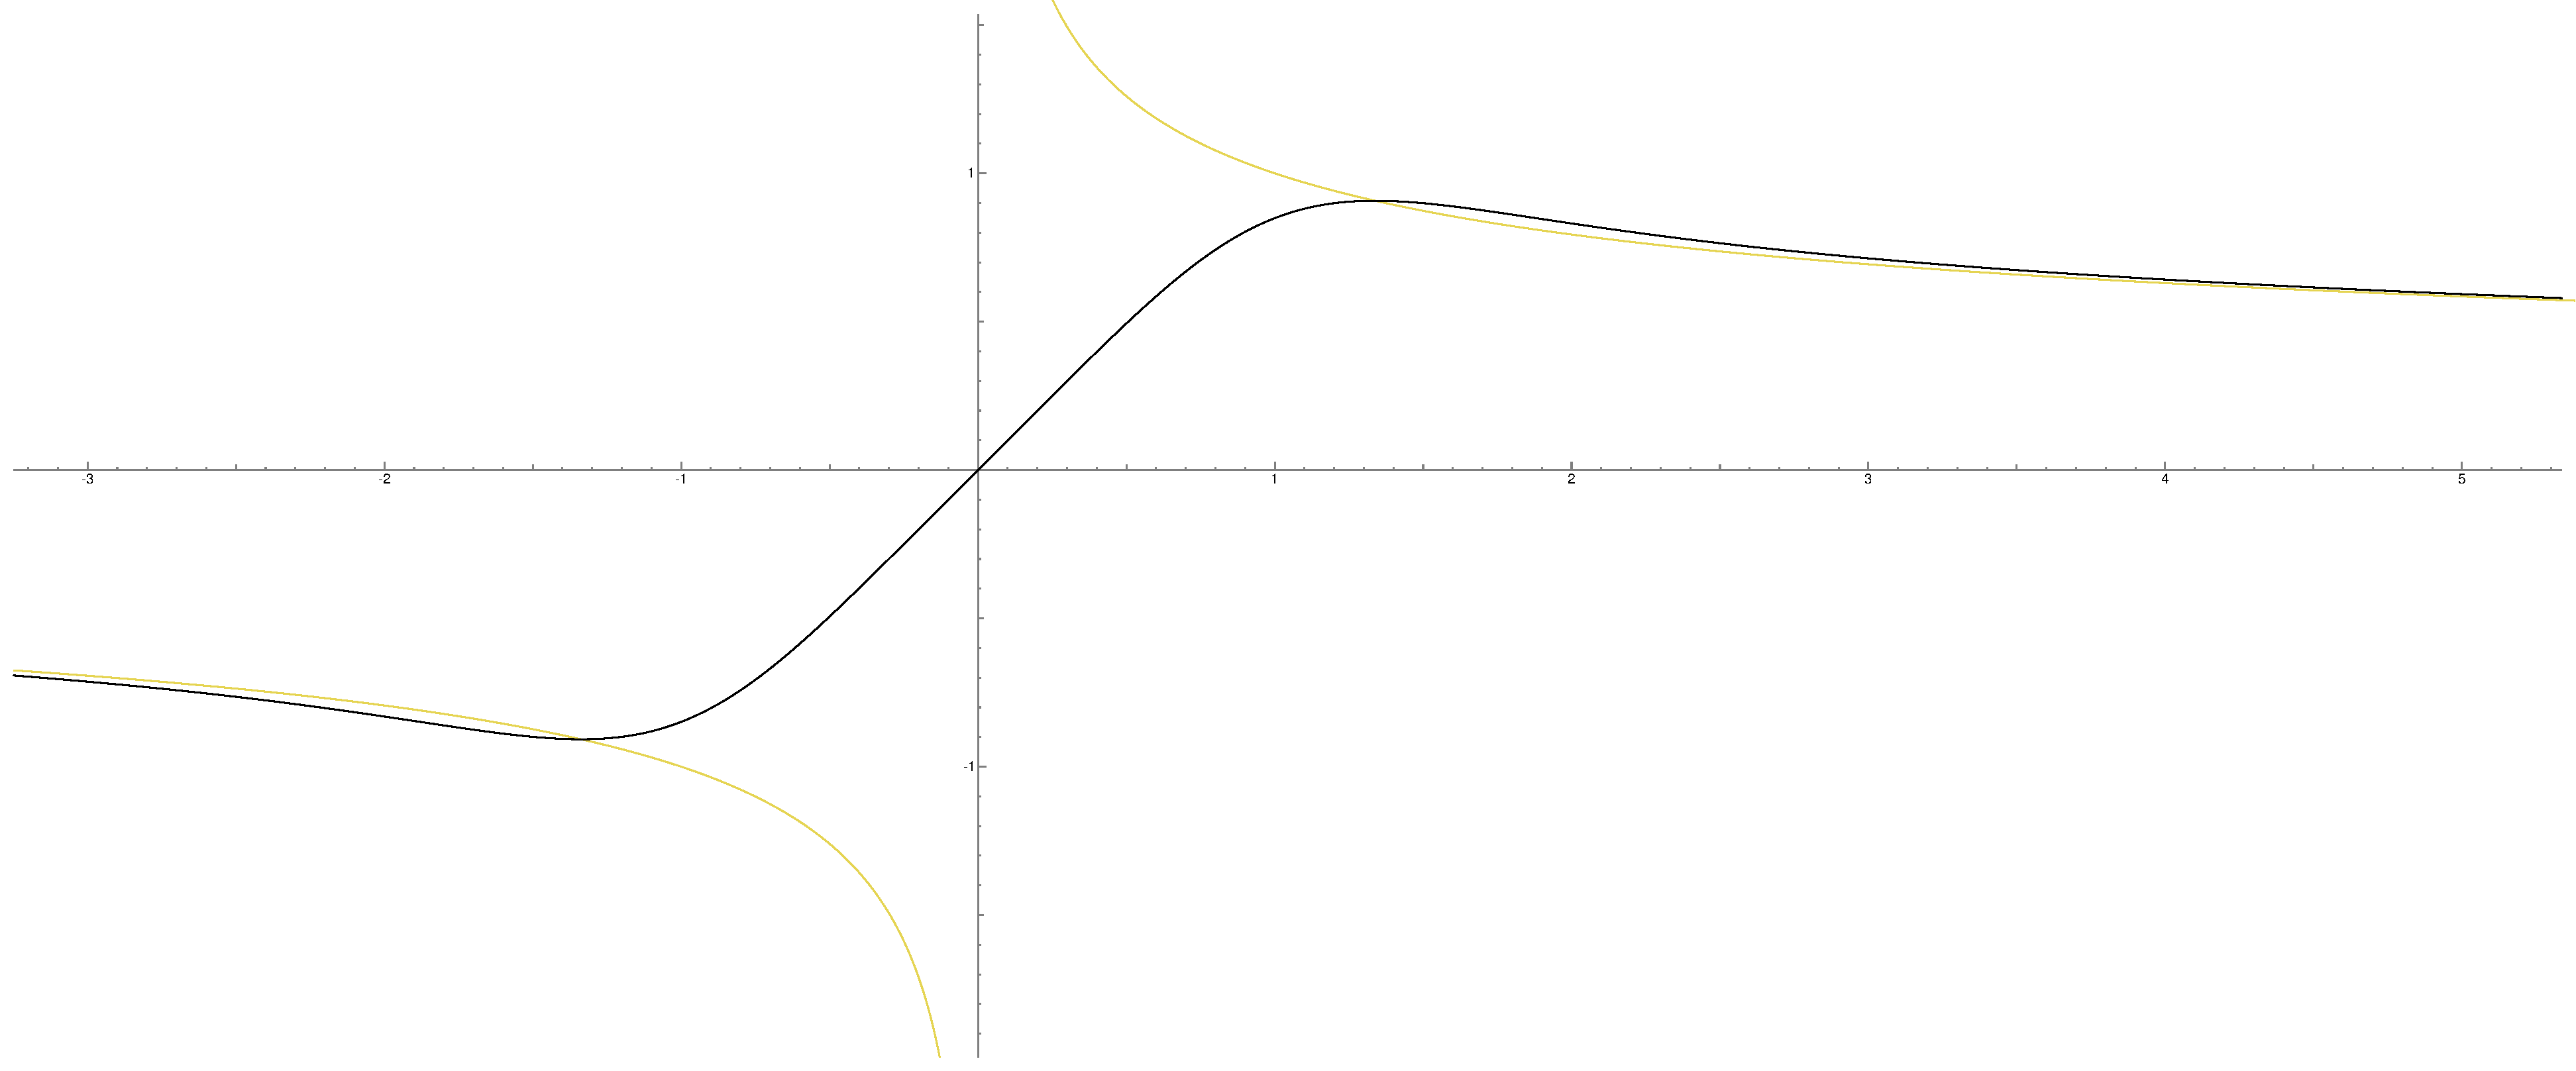
\includegraphics[width=0.8\textwidth]{ex843.pdf}
\caption{Il grafico della soluzione del problema di Cauchy nell'esempio~\ref{ex843}
\ifwidemargin\\\\\fi%
\usebox{\qrexoqt}}
\label{fig:ex843}
\end{figure}
%
\begin{example}\label{ex843}
Si consideri il seguente problema di Cauchy
\[
\begin{cases}
  u'=1-x u^3\\
  u(0)=0
\end{cases}
\]
ammette una soluzione $u(x)$ definita su tutto $\RR$.
\end{example}
%
\begin{proof}[Svolgimento.]
Posto $f(x,y)=1 - xy^3$ abbiamo che $f$ si annulla sul grafico della
funzione $u_0(x)=1/\sqrt[3] x$. Per $x>0$ la soluzione è crescente
quando si trova al di sotto della funzione $u_0$ ed è decrescente
quando si trova al di sopra. Inoltre essendo $u_0'<0$ le soluzioni possono
attraversare la funzione $u_0(x)$ solo passando da sotto a
sopra.

Sia $u(x)$ la soluzione del problema di Cauchy in questione, definita su
un intervallo massimale $I$. Il dato
iniziale è $(0,0)\in \{f>0\}$. Dunque la soluzione risulta essere
strettamente crescente in un intorno di $0$.

Vogliamo dimostrare innanzitutto che necessariamente la soluzione
incontra entrambi i rami del grafico di $u_0(x)$. Sia infatti
$\eps>0$ sufficientemente piccolo da appartenere all'intervallo
$I$ di
esistenza della soluzione e sia $\delta=u(\eps)$.
Consideriamo il compatto $K=\{(x,y):
\eps/2 \le x \le 1/\delta^2,\ 0\le y\le 1/\sqrt[3]{x}\}$. Il punto
$(\eps,u(\eps))$ è interno al compatto $K$ ma la soluzione deve
uscire dal compatto
per un qualche $x>\eps$.
La soluzione però non può toccare la
retta $y=0$ in quanto all'interno del compatto rimane sempre positiva
e crescente.
Non può neanche toccare il segmento verticale
$x=1/\delta^2$, $y\in[0,\delta]$ in quanto $u(\eps)=\delta$ e per
$x>0$ la soluzione è strettamente crescente.
Dunque necessariamente
la soluzione deve incontrare il grafico della funzione
$u_0(x)=1/\sqrt[3]{x}$ in un punto $\bar x>0$.

Nel punto $x=\bar x$ la soluzione $u(x)$ attraversa la curva
$u_0(x)$. Infatti in tale punto $u'(\bar x)=0$ mentre $u_0'(\bar
x)<0$.
Dunque in un intorno destro di $\bar x$ la soluzione si trova
al di sopra della curva $u_0(x)$ e quindi risulta essere decrescente
(in $\bar x$ la soluzione presenta un massimo relativo).

Il Teorema~\ref{nonpassa} garantisce inoltre che la soluzione non
può più riattraversare il grafico della funzione $u_0$ in quanto
$u'_0<0$. Dunque la soluzione è decrescente e limitata.
Dunque (usando come al solito la proposizione~\ref{prop:edo_massimale})
possiamo dedurre che la soluzione massimale è definita per ogni $x>0$.

Un ragionamento analogo si fa per $x<0$ ottenendo l'esistenza globale
della soluzione.
\end{proof}

\begin{example}
Dimostriamo che il problema di Cauchy
\[
\begin{cases}
	u' = -x(u^3 - \sin x) \\
	u(0) = 0
\end{cases}
\]
ammette una soluzione $u(x)$ definita su tutto $\RR$.
\end{example}
%
\begin{proof}
Sia $u(x)$ la soluzione massimale del problema di Cauchy
definita su un intervallo massimale $I$.

Mostriamo innanzitutto che $\vert u(x) \vert < 2$ per ogni $x\in
I$.
Infatti per $x>0$ sulla curva $u_1(x)=2$ si ha $f(x,2) = -x
(8-\sin x) < -x < 0 = u_1'(x)$.
Dunque per il Teorema~\ref{nonpassa} la
soluzione per $x>0$ non può mai attraversare la retta
$y=2$.
Discorso analogo si fa per la retta $y=-2$ e anche per $x<0$
mostrando che il grafico della  soluzione non può mai toccare le
rette $y=2$ e $y=-2$ né per $x>0$ né per $x<0$
e che quindi $u(x)$ risulta limitata (in realtà si
può essere più precisi e mostrare che $\vert u(x)\vert \le 1$).

A questo punto si applica, come al solito, il Teorema~\ref{prop:edo_massimale} ai
compatti $K_M=[-M,M]\times[-2,2]$ mostrando che la soluzione deve
avere esistenza globale.
\end{proof}

\subsection{teoremi di confronto}

\begin{theorem}
Sia $I\subset \RR$ un intervallo su cui sono definite due funzioni derivabili
$f(x)$ e $g(x)$.
Siano $x_1<x_2$ due punti di $I$. Se $f(x_1)<g(x_1)$ e $f(x_2)>g(x_2)$
allora esiste un punto $\bar x \in (x_1,x_2)$ tale che $f(\bar
x)=g(\bar x)$ e $f'(\bar x)\ge g'(\bar x)$.
\end{theorem}

\begin{theorem}
Consideriamo due funzioni $u(x)$ e $v(x)$ soluzioni dei rispettivi
problemi di Cauchy
\[
\begin{cases}
  u'(x)  = f(x,u(x))\\
  u(x_0) = u_0
\end{cases}
\qquad
\begin{cases}
  v'(x) = g(x,v(x))\\
  v(x_0) = v_0
\end{cases}
\]
su un intervallo $I$ che contiene il punto $x_0$.
Sia $\Omega\subset \RR^2$ un sottoinsieme degli insiemi di definizione
di $f$ e $g$ tale che i grafici delle soluzioni $u(x)$ e $v(x)$ siano
contenuti in $\Omega$ al variare di $x\in I$.
Supponiamo che per ogni $(x,y)\in\Omega$ si abbia $f(x,y)<g(x,y)$.
Allora per ogni $x\in I$, $x> x_0$ si ha $u(x)< v(x)$ mentre per ogni
$x\in I$, $x<x_0$ si ha $u(x)>v(x)$.
\end{theorem}

\begin{theorem}
Sia $f\colon (x_0,+\infty)\to \RR$ una funzione di classe
$C^1$ tale
che il limite
\[
  \lim_{x\to +\infty} f'(x) = \ell
\]
esiste, finito o infinito. Se $\ell\neq 0$ allora $f$ non può avere
un asintoto orizzontale per $x\to +\infty$.
\end{theorem}


\appendix
\chapter{Listati}

Il seguente codice è scritto in \emph{python 3}%
\mymargin{python 3}\index{python 3}
un linguaggio di programmazione
molto utilizzato per il calcolo numerico e scientifico.

\lstset{% general command to set parameter(s)
  language=python,
  basicstyle=\small\ttfamily, % print whole listing small
  keywordstyle=\color{black}\bfseries,
  % underlined bold black keywords
  identifierstyle=, % nothing happens
  commentstyle=\color{black!50}, % white comments
  stringstyle=\color{Maroon}\ttfamily, % typewriter type for strings
  showstringspaces=false} % no special string spaces

\section{bisection.py}

Vedi esempio~\ref{ex:75445}.
\myshortqrcode{bisection}{github}{bisection.py}
\label{code:bisection}
\lstinputlisting{code/bisection.py}

\section{napier.py}

Vedi Figura~\ref{fig:napier}.
\myshortqrcode{napier}{github}{napier.py}
\label{code:napier}
\lstinputlisting{code/napier.py}

\section{series.py}

Vedi esempio~\ref{ex:52573}.
\myshortqrcode{series}{github}{series.py}
\label{code:series}
\lstinputlisting{code/series.py}

\section{compute\_e.py}

Vedi tabella~\ref{fig:cifre_e}.
\myshortqrcode{computee}{github}{compute_e.py}
\label{code:compute_e}
\lstinputlisting{code/compute_e.py}

\section{compute\_pi.py}

Vedi esercizio~\ref{ex:cifre_pi}.
\myshortqrcode{computepi}{github}{compute_pi.py}
\label{code:compute_pi}
\lstinputlisting{code/compute_pi.py}

\section{Mandelbrot.py}

Vedi figura~\ref{fig:mandelbrot}.
\myshortqrcode{Mandelbrot}{github}{Mandelbrot.py}
\label{code:Mandelbrot}
\lstinputlisting{code/Mandelbrot.py}

\section{Koch.py}

Vedi figura~\ref{fig:koch}.
\myshortqrcode{Koch}{github}{Koch.py}
\label{code:Koch}
\lstinputlisting{code/Koch.py}

\section{Fourier.py}

Vedi figura~\ref{fig:fourier}
\myshortqrcode{Fourier}{github}{Fourier.py}
\label{code:Fourier}
\lstinputlisting{code/fourier.py}


\nocite{forallx}
\nocite{Giusti}
\nocite{Courant}
\nocite{Marcellini}
\nocite{Rudin}
\nocite{PaganiSalsa}
\bibliography{biblio}
\bibliographystyle{plain}

\printindex
\end{document}
